\documentclass[a4paper,twoside]{report}

\usepackage[a4paper,top=2cm,bottom=2cm,left=2.5cm,right=1.5cm]{geometry} 

\usepackage[fontsize=11pt]{scrextend}

\usepackage[english]{babel}

\usepackage[fixlanguage]{babelbib}

\usepackage{minted}
\usepackage{makeidx} 
\usepackage{csquotes}

\usepackage[utf8]{inputenc}
% UTF-8 character mappings for pdfLaTeX (requires \usepackage[utf8]{inputenc}).
% Replacement commands must stay environment-free so they work inside verbatim.

\usepackage{tikzsymbols}
\usepackage{textcomp}
\usepackage{CJKutf8}

\newsavebox{\UnicodeHanBox}
\newsavebox{\UnicodeMusicalGClefBox}

\AtBeginDocument{%
  \sbox{\UnicodeHanBox}{\begin{CJK}{UTF8}{gbsn}^^e6^^bc^^a2\end{CJK}}%
  \sbox{\UnicodeMusicalGClefBox}{%
    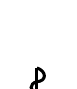
\begin{tikzpicture}[scale=0.07, baseline=-0.65ex]
      \draw[line width=1.1pt] (0,-2.2) -- (0,3.2);
      \draw[line width=1.1pt]
        (0,3.2) .. controls (1.8,2.6) and (1.8,0.8) .. (0,0.7)
        .. controls (-1.4,0.4) and (-1.4,-1.1) .. (0,-1.3);
    \end{tikzpicture}%
  }%
}

% Greek letters
\DeclareUnicodeCharacter{0398}{\ensuremath{\Theta}}
\DeclareUnicodeCharacter{03C0}{\ensuremath{\pi}}

% Symbols used in encoding / Unicode teaching examples
\DeclareUnicodeCharacter{2603}{\Snowman}
\DeclareUnicodeCharacter{1F600}{\dSmiley}
\DeclareUnicodeCharacter{6F22}{\usebox{\UnicodeHanBox}}
\DeclareUnicodeCharacter{1D11E}{\usebox{\UnicodeMusicalGClefBox}}
\DeclareUnicodeCharacter{0301}{\textasciiacute}

% Punctuation
\DeclareUnicodeCharacter{2014}{---}
\DeclareUnicodeCharacter{2019}{'}
\DeclareUnicodeCharacter{201C}{``}
\DeclareUnicodeCharacter{201D}{''}

\usepackage{pifont}
\usepackage[T1]{fontenc}
\usepackage{amssymb}
\usepackage{graphicx}
\usepackage{subcaption}
\captionsetup{font=small}
\captionsetup{width=0.85\textwidth}
\usepackage{booktabs}
\usepackage{array}
\usepackage[table]{xcolor}

\usepackage{rotating}
\usepackage{fancyhdr}               
\usepackage{bbm}
\usepackage{amsmath}
\usepackage{amsthm}         
\usepackage{diagbox}
\usepackage{wrapfig}

\usepackage[most]{tcolorbox} % loads tikz under the hood
\tcbuselibrary{minted}
\usepackage{etoolbox}        % for \docsvlist (comma lists)

\usepackage{xcolor}
\usepackage{multirow}
\definecolor{codebg}{RGB}{245,245,245}

% optional: add LoF/LoT to ToC
\usepackage[nottoc]{tocbibind}
\usepackage{makecell}
\usepackage{graphicx}
\usepackage[dvipsnames,table]{xcolor} 
\usepackage{listings}          
\usepackage{hyperref}     
\usepackage[normalem]{ulem}
\usepackage{framed}
\usepackage{csquotes}
\usepackage{anyfontsize}
\usepackage{float}
\usepackage{pgfplots}
\usepackage{tikz}
\usepackage[nameinlink]{cleveref}
\usepackage[justification=centering]{caption}
\usetikzlibrary{shapes.geometric, fit,positioning,calc,arrows.meta,backgrounds}
\usepackage{import}
\subimport{layers/}{init.tex}

\newcommand{\cmark}{\ding{51}} % ✓
\newcommand{\xmark}{\ding{55}} % ✗ 

\makeatletter
\setlength{\@fptop}{0pt}
\makeatother

\pgfplotsset{width=7cm,compat=1.9}

\def\ImgColor{rgb:yellow,2.5;red,5;white,2.5}
\def\InputColor{blue!20}
\def\ConvColor{rgb:yellow,5;red,2.5;white,5}
\def\ConvReluColor{rgb:yellow,5;red,5;white,5}
\def\PoolColor{rgb:red,1;black,0.3}
\def\UnpoolColor{rgb:blue,2;green,1;black,0.3}
\def\FcColor{rgb:blue,5;red,2.5;white,5}
\def\FcReluColor{rgb:blue,5;red,5;white,4}
\def\SoftmaxColor{rgb:magenta,5;black,7}
\def\SumColor{rgb:blue,1;black,0.3}
\def\OtherColor{rgb:blue,2;red,2.5;white,5}   

\pgfplotsset{
    datasetstype/.style={
    legend style={draw=none, font=\small},
    legend cell align=left,
    legend pos=north east,
    ylabel style={align=center, font=\tiny},
    xlabel style={align=center, font=\tiny},
    x tick label style={font=\tiny},
    y tick label style={font=\tiny},
    scaled ticks=false,
    every axis plot/.append style={thick},
    },
    dualchartstyle/.style={
    legend style={draw=none, font=\small},
    legend cell align=left,
    legend pos=north east,
    ylabel style={align=center, font=\bfseries\boldmath},
    xlabel style={align=center, font=\bfseries\boldmath},
    x tick label style={font=\bfseries\boldmath},
    y tick label style={font=\bfseries\boldmath},
    scaled ticks=false,
    every axis plot/.append style={thick},
    }
}

% One consistent chip style:
\newtcbox{\bluechip}{on line,
  colback=blue!10,
  colframe=blue!50!black,
  boxrule=0.4pt,
  arc=2pt,
  left=1pt, right=1pt, top=0.1ex, bottom=0.1ex, % << way less padding
  tcbox raise base,
  enhanced,
  before upper=\sffamily\footnotesize
}

\newtcbox{\redchip}{on line,
  colback=red!10,
  colframe=blue!50!black,
  boxrule=0.4pt,
  arc=2pt,
  left=1pt, right=1pt, top=0.1ex, bottom=0.1ex, % << way less padding
  tcbox raise base,
  enhanced,
  before upper=\sffamily\footnotesize
}

\newtcbox{\yellowchip}{on line,
  colback=yellow!10,
  colframe=blue!50!black,
  boxrule=0.4pt,
  arc=2pt,
  left=1pt, right=1pt, top=0.1ex, bottom=0.1ex, % << way less padding
  tcbox raise base,
  enhanced,
  before upper=\sffamily\footnotesize
}


\pagestyle{fancy}
\fancyhf{}
\lhead{{\fontsize{8}{11}\selectfont\nouppercase{\rightmark}}}
\rhead{\textbf{\thepage}}
\fancyfoot{}
\setlength{\headheight}{14pt}

% Rimuove il numero di pagina all'inizio dei capitoli
\fancypagestyle{plain}{
  \fancyfoot{}
  \fancyhead{}
  \renewcommand{\headrulewidth}{0pt}
}

% Stile del codice
\lstdefinestyle{codeStyle}{
    % Colore dei commenti
    commentstyle=\color{teal},
    % Colore delle keyword
    keywordstyle=\color{Magenta},
    % Stile dei numeri di riga
    numberstyle=\tiny\color{gray},
    % Colore delle stringhe
    stringstyle=\color{violet},
    % Dimensione e stile del testo
    basicstyle=\ttfamily\footnotesize,
    % newline solo ai whitespaces
    breakatwhitespace=false,     
    % newline si/no
    breaklines=true,                 
    % Posizione della caption, top/bottom 
    captionpos=b,                    
    % Mantiene gli spazi nel codice, utile per l'indentazione
    keepspaces=true,                 
    % Dove visualizzare i numeri di linea
    numbers=left,                    
    % Distanza tra i numeri di linea
    numbersep=5pt,                  
    % Mostra gli spazi bianchi o meno
    showspaces=false,                
    % Mostra gli spazi bianchi nelle stringhe
    showstringspaces=false,
    % Mostra i tab
    showtabs=false,
    % Dimensione dei tab
    tabsize=2
} \lstset{style=codeStyle}

% Stile di codice per dimensioni maggiori, in cui ho avuto bisogno di un testo più picolo (ad esempio se si vuole inserire del codice che ha linee molto lunghe). Per usare questo stile piuttosto che il precedente, usare 

% \lstset{style=longBlock}
%  % inserire il codice...
% \lstset{style=codeStyle}

% Il secondo comando consente di tornare allo stile precedente 
\lstdefinestyle{longBlock}{
    commentstyle=\color{teal},
    keywordstyle=\color{Magenta},
    numberstyle=\tiny\color{gray},
    stringstyle=\color{violet},
    basicstyle=\ttfamily\scriptsize,
    breakatwhitespace=false,         
    breaklines=true,                 
    captionpos=b,                    
    keepspaces=true,                 
    numbers=left,                    
    numbersep=5pt,                  
    showspaces=false,                
    showstringspaces=false,
    showtabs=false,                  
    tabsize=2
} \lstset{style=codeStyle}

% Togliendo il commento al comando che segue, si inseriscono nella bibliografia anche le fonti presenti in Bibliography.bib ma non citati direttamente con il comando \cite
% \nocite{*}

% Margini prima e dopo blocchi di codice, per avere più distanza
\lstset{aboveskip=20pt,belowskip=20pt}

\definecolor{royalgreen}{HTML}{006400} % Dark Green
% OR for a slightly more modern "Emerald Forest"
\definecolor{forestbluegreen}{HTML}{004d40}

\hypersetup{
    colorlinks=true,
    linkcolor=royalgreen,
    citecolor=royalgreen,
    urlcolor=royalgreen
}


% Aggiunti definizioni, teoremi, linea e listing
\newtheorem{definition}{Definizione}[section]
\newtheorem{theorem}{Teorema}[section]
\providecommand*\definitionautorefname{Definizione}
\providecommand*\theoremautorefname{Teorema}
\providecommand*{\listingautorefname}{Listing}
\providecommand*\lstnumberautorefname{Linea}

\raggedbottom

%\newcommand{\cgs}[1]{{\textcolor{brown}[\textcolor{red}{\bf{GS: }}{ \textcolor{brown}{#1]}}}}             
%\newcommand{\cmc}[1]{{\textcolor{blue}[\textcolor{magenta}{\bf{MC: }}{ \textcolor{blue}{#1]}}}}


% --- MODERN LANGUAGE BADGE ---
\newcommand{\langbadge}[1]{%
    \tcbox[on line,
           arc=0.5mm,
           boxrule=0.1mm,
           colback=gray!90!black,
           colframe=gray!90!black,
           size=minimal,
           left=1.5mm,
           right=1.5mm,
           top=0.6mm,
           bottom=0.6mm]%
           {\textcolor{white}{\sffamily\bfseries\tiny\texttt{</>}\,\MakeUppercase{#1}}}%
}

% --- REFINED MINIMALIST CODE BLOCK STYLE (WITH OPTIONAL OVERRIDES) ---
% We change the arguments to 4, with the first [1] being optional and defaulting to empty.
\newtcblisting[auto counter, number within=section]{codebox}[4][]{%
    % #1 = Optional Minted overrides (e.g., linenos=false), defaults to empty
    % #2 = Language, #3 = Caption, #4 = Label/Index entry
    colback=gray!2!white,
    colframe=gray!40!black,
    boxrule=0.2mm,                
    borderline west={1mm}{0mm}{gray!60!black}, 
    fonttitle=\bfseries\sffamily\footnotesize,  
    coltitle=gray!90!black,
    colbacktitle=gray!10!white,
    % Prepends the language badge directly onto the left of the title tab
    title={\langbadge{#2}\hspace{1.5mm}Listing \thetcbcounter: #3},
    enhanced,
    attach boxed title to top left={yshift=-2mm, xshift=2mm},
    boxed title style={
        colframe=gray!40!black,
        boxrule=0.2mm,
        arc=1mm
    },
    label={lst:#4},
    index={#4}, 
    left=11mm, 
    listing engine=minted,
    minted language=#2,
    minted options={
        linenos=true,             % ON by default
        numbersep=12pt,           
        fontsize=\small,
        gobble=0,
        breaklines=true,
        #1                        % Any option passed to #1 overrides the defaults!
    },
    listing only
}


% --- REFINED FLAT INPUT BOX ---
\newtcolorbox{inputbox}[1]{
    colback=black!75,          
    colframe=black!75,
    boxrule=0.2mm,               
    coltext=white,              
    fonttitle=\bfseries\sffamily\scriptsize,   
    title=#1,
    size=small,
    arc=0mm, 
    top=2mm,
    bottom=2mm,
    after=\vspace{-0.2mm}       
}

% --- REFINED FLAT OUTPUT BOX ---
\newtcolorbox{iobox}[1]{
    colback=black!90,
    colframe=black!90,
    boxrule=0.2mm,               
    coltext=green!40!white,     
    fonttitle=\bfseries\sffamily\scriptsize,   
    title=#1,
    size=small,
    arc=0mm, 
    top=2mm,
    bottom=2mm
}

\definecolor{slatenavy}{HTML}{1A2B3C}
\definecolor{offwhite}{HTML}{FAFAFA}
\definecolor{mutedgray}{HTML}{555555}

% -----------------------------------------------------------------
\begin{document}



\begin{titlepage}
    \clearpage
    \thispagestyle{empty}

    % Establish the flat, cold, off-white background canvas
    \begin{tikz}[remember picture, overlay]
        \fill[offwhite] (current page.south west) rectangle (current page.north east);
    \end{tikz}

    % Severe flush-left alignment for the primary typographic stack
    \begin{flushleft}
        \vspace*{1.5cm}

        % Sharp structural accent line
        {\color{slatenavy}\hrule height 2.5pt}
        \vspace*{0.8cm}

        % Main Title: Massive, clean, aggressive sans-serif
        {\fontsize{34}{45}\selectfont\sffamily\bfseries\color{black} PROGRAMMING IN PYTHON} \\[0.4cm]
        
        % Subtitle: Monospace font indicating the engineering focus
        {\fontsize{13}{18}\selectfont\ttfamily\color{slatenavy} assist. Sorin Milutinovici} \\[1.2cm]
        
    
        \vspace*{5.5cm}

        % Minimalist vertical geometric marker to balance the negative space
        
\begin{tikzpicture}
            \fill[slatenavy!30] (0,0) rectangle (0.08cm, 2.5cm);
        \end{tikzpicture}

    \end{flushleft}

    \vfill

    % Severe flush-right alignment for institutional metadata
    \begin{flushright}
        \ttfamily\fontsize{9}{14}\selectfont\color{black}
        \rule{6cm}{0.5pt} \\[0.3cm]
        \textbf{TITU MAIORESCU UNIVERSITY} \\[0.1cm]
        \textbf{DEPARTMENT OF COMPUTER SCIENCE} \\[0.1cm]
        \color{mutedgray}RELEASE: MAY 2026
    \end{flushright}

    \vspace*{0.5cm}
\end{titlepage}

\tableofcontents

\clearpage

%=== Main content placeholder ===%
\chapter{Introduction}

Python is a magnificent dynamic illusion layered over a massive, hyper-optimized C application. It is the ultimate "glue" language, but an absolute nightmare for hardware cache efficiency. It trades CPU cycles and memory density wholesale for human iteration speed. For an engineer raised on bare metal, looking under Python's hood reveals a fascinating paradox: a language that presents a clean, minimalist facade to the programmer, while forcing the underlying runtime framework to work furiously behind the scenes to maintain that illusion.

\chapter{Execution Architecture: From C Processes to Python Runtime Semantics}

A Python course can begin with Python syntax, but that approach leaves the student with a dangerous illusion: that programming is mainly the act of arranging visible language constructs. It is not. Programming is the act of describing computations that must eventually be represented, loaded, scheduled, executed, interrupted, resumed, and stored inside a real machine. A student who only learns the visible syntax of Python may become comfortable writing small scripts, but will often remain unable to explain why variables behave differently from C variables, why function calls create frames, why lists store references rather than raw values, why exceptions can unwind several calls at once, why generators can resume after yielding, or why asynchronous programs can handle many waiting tasks without using many CPU cores.

This chapter therefore starts below Python. It begins with the native execution model, using C as the reference architecture. This is not a detour. It is the baseline. C shows the traditional path clearly: source code becomes object code, object code becomes an executable, the operating system loader maps that executable into memory, the process receives a stack and heap, and the CPU executes machine instructions from the text segment. Once this model is understood, Python can be explained honestly: not as magic, not as ``just interpreted'', and not as a loose collection of convenient syntax rules, but as a runtime-hosted language executed inside a native interpreter process.

The analogy is simple. One may learn to move a car in a parking lot without understanding roads, intersections, lanes, bridges, roundabouts, traffic lights, and right-of-way rules. But that person is not yet a competent driver. In the same way, one may learn to print strings, write loops, and define functions without understanding processes, memory, frames, objects, bytecode, and runtime scheduling. That person can operate the surface of the language, but cannot yet understand the execution environment in which real programs live.

The first section of the chapter establishes the native process model. It explains what a program is, what a process is, what the operating system kernel does, how compilation transforms C source code into executable form, how loading creates an active virtual address space, and how memory is divided into text, data, BSS, heap, and stack regions. This gives the student a concrete mental model for compiled execution: where instructions live, where variables live, how function calls use stack frames, why heap allocation must be managed, and why the operating system remains in control even when the program is native machine code.

The second section introduces process virtual machines and interpreted runtimes. This is where the Python execution model becomes visible. When a Python file is run, the operating system does not load that file as a native executable. It loads the CPython executable. The Python file is input to a runtime. CPython parses it, compiles it to bytecode, creates code objects and frames, allocates Python objects, and executes virtual instructions through an interpreter loop. This section also compares CPython with the JVM, V8, PHP, and Bash, because the word \emph{interpreted} is too vague to be useful unless we separate source interpretation, bytecode interpretation, opcode execution, JIT compilation, host-provided event loops, and command dispatch.

The third section studies modern procedural extensions: callbacks, anonymous functions, closures, generators, coroutines, and asynchronous execution. These constructs are placed here because they only make full sense after the runtime model is clear. A closure requires preserved lexical state beyond an ordinary stack frame. A generator requires suspended execution state. A coroutine requires controlled resumption. An asynchronous task requires the runtime or event loop to remember what should continue after an external event becomes ready. These are not just elegant language features. They are consequences of treating code, frames, continuations, and waiting operations as runtime-managed structures.

The chapter is therefore laid out as a bridge. It moves from native execution to runtime-hosted execution, and then from ordinary procedures to runtime-managed control flow. This order is deliberate. Python's variable model cannot be explained well before the object model. The object model cannot be explained well before the heap and references. Python frames cannot be explained well before native stack frames. Python bytecode cannot be explained well before machine code and instruction streams. Async execution cannot be explained well before scheduling, blocking, and suspended state. The chapter builds these dependencies in the order in which they become intelligible.

The purpose is not to turn a Python book into an operating systems book or a compiler construction book. The purpose is to give Python the execution context it deserves. A serious programming language is not only its syntax. It is a complete execution architecture. Python becomes much easier to understand when seen as a managed runtime layered above the native process model inherited from systems such as C.

This approach also protects the student from misleading simplifications. Python variables are not C boxes. Python assignment is not memory copying. Python functions are not only named source blocks. Python exceptions are not only error messages. Python generators are not lists. Python concurrency is not automatically parallelism. Each of these facts becomes clear only when the underlying architecture is visible.

For that reason, this chapter is not preliminary decoration. It is the foundation of the course. A student who understands this chapter will read the rest of Python differently. Syntax will no longer be memorized as isolated rules. It will be interpreted as surface notation for deeper mechanisms: objects, bindings, frames, bytecode, namespaces, managed memory, and runtime-controlled execution.

\section{Operating Systems, Programs, and Process Mechanics}

Before Python can be understood as a programming language, it is useful to understand what happens underneath any language when code is executed. A program does not run in isolation, directly on the physical machine, simply because a programmer wrote instructions in a source file. Between source code and execution there are several layers: executable files, operating-system loaders, process memory layouts, virtual address spaces, kernel scheduling, and hardware-supported resource isolation. These layers form the execution environment in which both C programs and Python programs eventually run.

This section uses the traditional C execution model as the reference point. C is useful here because it exposes the native path clearly: source code is transformed through preprocessing, compilation, assembly, and linking into a binary executable; the operating system loads that executable; the loader maps code and data into virtual memory; the process receives a stack, heap, registers, arguments, and resources; and the CPU begins executing machine instructions from the program's text segment. This path gives us a concrete model of what a native program is and how it becomes an active process.

The main distinction developed in this section is the distinction between a \emph{program} and a \emph{process}. A program is a stored blueprint: a file or collection of files containing instructions, data, and metadata. A process is the running instance created from that blueprint. The process has its own virtual address space, its own stack, heap, mapped code regions, open resources, and scheduling identity. This distinction is essential because Python code will later be shown not as a native executable in the ordinary C sense, but as input executed inside an already running interpreter process.

We will also examine the role of the operating system kernel. The kernel is the privileged layer that creates processes, maps memory, protects address spaces, handles traps and system calls, schedules CPU time, and mediates access to files, devices, and other resources. Even a C program compiled to machine code does not own the machine. It runs inside a boundary created and enforced by the operating system. Its pointers are process-virtual addresses, its files are kernel-managed resources, and its execution can be suspended and resumed by the scheduler.

The memory layout of a native process is another central theme. We will separate the text segment, data segment, BSS, heap, and stack. These regions explain where machine instructions live, where global and static variables are stored, where dynamic allocations are created, and how function calls produce stack frames. This is the model that C programmers usually approach directly through pointers, arrays, \texttt{malloc()}, \texttt{free()}, function calls, and local variables.

Finally, we will connect process mechanics to multitasking. Modern operating systems do not run only one program until completion. They time-slice CPU resources, suspend and resume processes or threads, switch execution contexts, and distribute work across multiple cores. This explains the difference between processes and threads, between isolation and shared memory, and between operating-system scheduling and runtime-level scheduling. That last transition prepares the ground for later Python concepts such as generators, coroutines, event loops, and asynchronous execution.

The purpose of this section is not to turn the chapter into an operating-systems course. The purpose is to establish the execution model that Python will modify, abstract, and partially hide. Once the native C model is clear, the Python model becomes easier to describe precisely: the operating system runs the CPython executable as a normal native process, while the user's Python source file is parsed, compiled to bytecode, and executed inside that process by the Python runtime.


\subsection{Foundations of Execution Architecture}
\subsubsection{What is a Program? The Static Binary Blueprint and Executable Formats (ELF on Linux, PE/COFF on Windows)}

A program is a stored description of future execution. Before it runs, it is not yet an active computation. It is only data placed somewhere in persistent storage: on a disk, inside an archive, inside a package, or inside another executable container. In the native compiled model, such as the model normally used by C, the final program is usually an executable binary file. This file contains machine instructions, static data, metadata, relocation information, and structural descriptions that tell the operating system how the file must be loaded into memory.

This distinction is important. A program is not the same thing as a process. A program is the static object. A process is the active execution instance created from that object. The same executable file can be launched many times, producing many independent processes. Each process receives its own execution state: virtual memory mappings, stack, heap, open resources, CPU register state, and scheduling identity. The executable file is therefore only the blueprint from which the operating system constructs a running process.

In C, after preprocessing, parsing, compilation, assembly, and linking, the final result is commonly a binary executable. This binary is not just a flat sequence of CPU instructions. It has a formal file format. The operating system loader must be able to read this format, validate it, and map its parts into the future process address space. Two major executable format families are especially relevant:

\begin{itemize}
    \item \textbf{ELF} (\emph{Executable and Linkable Format}), used mainly on Linux and other Unix-like systems;
    \item \textbf{PE/COFF} (\emph{Portable Executable / Common Object File Format}), used on Windows.
\end{itemize}

These formats solve the same basic problem: they describe how a compiled program is organized so that the operating system can load it and the processor can execute it. The file must contain enough information for the loader to answer questions such as:

\begin{itemize}
    \item What processor architecture is this program compiled for?
    \item Where is the machine code stored inside the file?
    \item Which parts of the file must become readable, writable, or executable memory?
    \item What dynamic libraries are required?
    \item Where is the initial entry point of execution?
    \item What symbols or relocations must be resolved before execution can begin?
\end{itemize}

In an ELF executable, for example, the file contains an ELF header, program headers, sections, and segments. Sections are mainly useful during linking and analysis. Segments are especially important during execution because they describe what the operating system must map into memory. A typical executable contains a code area, often called the \texttt{text} segment, together with areas for initialized data, uninitialized data, read-only constants, dynamic linking information, and other runtime metadata.

On Windows, PE/COFF plays a similar role. A Windows executable file, usually ending in \texttt{.exe} or \texttt{.dll}, contains headers and tables that describe code sections, data sections, imported libraries, exported symbols, relocation information, and the program entry point. The exact structure is different from ELF, but the purpose is the same: the file is a structured contract between the compiler toolchain, the operating system loader, and the processor architecture.

The processor cannot execute an ELF file or a PE file as a whole. The file format is not itself the instruction stream. Instead, the operating system reads the file, interprets its metadata, maps selected parts into virtual memory, prepares the stack and other process structures, resolves required dynamic dependencies, and then transfers control to the program's entry point. Only after this loading phase do the machine instructions begin to execute.

This also explains why a native executable is tied to both an operating system format and a processor instruction set. A Linux ELF binary compiled for x86-64 cannot normally be launched directly as a Windows PE executable. A Windows PE executable compiled for x86-64 cannot directly run on an ARM processor without a compatibility or emulation layer. A native program must match both sides of the execution environment:

\begin{itemize}
    \item the \textbf{operating system}, because the loader must understand the executable format and system call conventions;
    \item the \textbf{processor architecture}, because the machine instructions must belong to the processor's instruction set.
\end{itemize}

This native model is the reference point for understanding why Python behaves differently. A Python source file, such as \texttt{script.py}, is also a program in the broad sense: it is a stored description of future execution. However, it is not normally an executable binary containing native machine instructions for the processor. The operating system does not load \texttt{script.py} in the same way it loads a C executable. Instead, the operating system loads the Python interpreter executable, such as \texttt{python} or \texttt{python.exe}. That interpreter is the native program. The Python source file becomes input data for that running interpreter process.

Therefore, in the C model, the programmer's source code is transformed into the native executable that the operating system loads. In the Python model, the interpreter is the native executable, while the user's Python file is interpreted, compiled to bytecode, and executed inside the runtime environment created by that interpreter. This difference is one of the central architectural transitions between C programming and Python programming.

\subsubsection{What is a Process? A Running Program with Its Own Virtual Address Space}

A process is a running instance of a program. If the program is the static blueprint stored on disk, the process is the active object created when the operating system loads that blueprint and gives it execution resources. A process is therefore not just the executable file copied into memory. It is a complete runtime container: it has memory mappings, an execution state, open resources, scheduling information, and a relationship with the operating system kernel.

The same program file can produce many processes. If the user starts the same executable three times, the disk file is still one file, but the operating system creates three separate processes. Each process has its own identity, usually represented by a process identifier, or PID. Each process also has its own execution state. One instance may be waiting for keyboard input, another may be writing to a file, and another may already be finished. They all come from the same program, but they are different runtime entities.

The most important property of a modern process is its \textbf{virtual address space}. From the point of view of the running program, memory appears as a large private address range. The program uses addresses as if it owned this memory directly. In reality, the operating system and the memory management unit (MMU) translate those virtual addresses into physical memory locations or into other backing storage mechanisms.

This gives every process an isolated view of memory. One process cannot normally read or write the memory of another process just by using an address. The address \texttt{0x100000} inside one process does not mean the same physical location as \texttt{0x100000} inside another process. The same virtual address can exist in many processes at the same time, but the operating system maps it differently for each one.

This isolation is one of the main differences between a simple program image and a real process. The executable file contains descriptions of code and data. The process contains mapped memory regions created from those descriptions, plus additional runtime regions created by the operating system and by the runtime libraries. A typical process address space contains regions such as:

\begin{itemize}
    \item a \textbf{text} or code region, containing executable machine instructions;
    \item read-only constant data;
    \item initialized global and static data;
    \item uninitialized global and static data, often called BSS;
    \item the \textbf{heap}, used for dynamic allocation;
    \item one or more \textbf{stacks}, used for function calls and local execution state;
    \item memory-mapped libraries;
    \item kernel-provided or runtime-provided auxiliary regions.
\end{itemize}

In a C program, this structure is visible through concepts such as global variables, local variables, pointers, \texttt{malloc()}, \texttt{free()}, and function call stack frames. A global variable may live in the data or BSS region. A local automatic variable usually lives in a stack frame. A dynamically allocated object usually lives on the heap. A pointer stores an address inside the process virtual address space.

The processor does not execute an entire process at once. At any exact moment, a hardware thread executes one instruction stream. For a process to run, the operating system scheduler assigns CPU time to it. The process then executes for a while, may be interrupted, may block while waiting for input or output, or may voluntarily give control back to the kernel through a system call.

To suspend and later resume a process, the operating system must preserve its execution context. This includes, among other things, the current instruction pointer, stack pointer, register values, scheduling state, and memory mapping information. When the scheduler later chooses the process again, this saved state is restored, and execution continues as if the process had not stopped. This save-and-restore operation is part of what makes multitasking possible.

A process also owns or references external resources. These resources are not only memory. A process may have:

\begin{itemize}
    \item open file descriptors or file handles;
    \item network sockets;
    \item environment variables;
    \item command-line arguments;
    \item loaded shared libraries;
    \item child processes;
    \item security credentials and permissions.
\end{itemize}

These resources are managed by the operating system. The process can request operations on them, but it normally does so through system calls or library wrappers around system calls. User code does not directly control the disk controller, network card, or physical memory. It asks the kernel to perform controlled operations.

This explains why the process is an operating-system object, not only a programming-language object. A C function, a Python function, or a Java method exists inside some runtime model, but the process itself is created and supervised by the operating system. The process is the boundary at which the operating system gives a running program memory isolation, resource ownership, and scheduling identity.

The process model also helps clarify what happens when Python code is executed. When the command

\begin{verbatim}
python script.py
\end{verbatim}

is launched, the operating system does not create a process directly from \texttt{script.py}. The file \texttt{script.py} is not normally a native executable file. Instead, the operating system creates a process from the native Python interpreter executable: \texttt{python} on Linux or \texttt{python.exe} on Windows. That interpreter process then opens the Python source file, parses it, compiles it to bytecode, and executes it inside the CPython runtime.

Therefore, in the Python case, there are two different levels that must not be confused. At the operating-system level, the running process is the CPython interpreter process. At the language level, the user's Python program is being executed inside that process. The Python program has its own Python-level objects, frames, namespaces, and bytecode execution state, but all of these live inside the memory and resource boundary of the interpreter process created by the operating system.

This is the key transition from C to Python. In C, the programmer's source code is compiled and linked into the native executable that becomes the process. In Python, the interpreter is the native executable that becomes the process, while the user's source file becomes input to a managed runtime already running inside that process.

\subsubsection{The Role of the Operating System Kernel: Supervisor Mode, Hardware Traps, System Calls, and Resource Isolation}

The operating system kernel is the privileged core of the operating system. It is the software layer that stands between ordinary programs and the physical machine. A user program does not normally control the processor, memory, disk, keyboard, network card, or display directly. Instead, it runs under restrictions imposed by the kernel and must request privileged operations through controlled entry points.

Modern processors usually separate execution into at least two privilege levels. The exact names differ across architectures, but the conceptual distinction is stable:

\begin{itemize}
    \item \textbf{user mode}, where ordinary application code runs with restricted permissions;
    \item \textbf{kernel mode} or \textbf{supervisor mode}, where the operating system kernel runs with privileged access to hardware and process management structures.
\end{itemize}

A C program, a Python interpreter process, a browser, or a text editor normally runs in user mode. User-mode code cannot directly modify page tables, program the disk controller, access arbitrary physical memory, or take control of another process. These restrictions are not just software conventions. They are enforced by the processor and the memory management unit.

The kernel runs in supervisor mode because it must perform operations that affect the whole system. It creates processes, schedules CPU time, maps virtual memory, handles files, communicates with devices, enforces permissions, and responds to hardware events. If every program could perform these operations directly, one incorrect pointer, one malicious write, or one infinite loop could damage the whole machine.

The transition from user mode to kernel mode happens through controlled mechanisms. One of the most important mechanisms is the \textbf{system call}. A system call is a request made by a user program to the kernel. For example, when a program wants to open a file, allocate more memory, write to the console, create a process, or send data through a socket, it eventually performs a system call.

From the programmer's point of view, this request is often hidden behind a library function. In C, a call such as \texttt{printf()} may eventually lead to a lower-level write operation. In Python, a call such as \texttt{print()} or \texttt{open()} eventually reaches operating-system services through the CPython runtime and the C standard library or platform APIs. The programmer does not normally write the raw system call instruction directly.

A system call requires a controlled change of privilege level. The processor must stop executing ordinary user code and enter kernel code at a known, valid entry point. This transition is not a normal function call. A normal function call stays inside the same privilege level and the same program address space. A system call crosses the boundary between the user program and the operating system kernel.

This boundary crossing is usually implemented using a special processor instruction or a similar architecture-specific mechanism. Conceptually, the program places a request number and arguments in agreed locations, then triggers the transition. The processor switches into supervisor mode and transfers control to the kernel. The kernel validates the request, checks permissions, performs the operation if allowed, places a result or error code where the user program can retrieve it, and then returns control to user mode.

Another important mechanism is the \textbf{hardware trap}. A trap is a controlled transfer of execution to the kernel caused by a special event. Some traps are intentionally triggered by programs, such as system calls. Others are caused by exceptional conditions during execution. Examples include division by zero, invalid memory access, illegal instructions, page faults, and breakpoints used by debuggers.

For example, if a C program dereferences an invalid pointer, the processor may detect that the virtual address is not mapped or is not accessible with the requested permissions. The processor then traps into the kernel. The kernel examines the situation. If the access is invalid, it may terminate the process and report a segmentation fault or access violation. If the access corresponds to a valid page that must be loaded or mapped, the kernel may repair the situation and resume the process.

This trap mechanism is central to virtual memory. A process believes it is using a private address space, but the mapping from virtual addresses to physical memory is controlled by the kernel and the MMU. When a process touches a memory page that is not currently available, the hardware can trap into the kernel. The kernel then decides whether the access is legal, whether the page should be loaded, or whether the process must be stopped.

The kernel therefore enforces \textbf{resource isolation}. Each process receives the illusion of private memory and controlled access to external resources. One process cannot normally overwrite another process's stack, corrupt another process's heap, close another process's files, or steal another process's network connection. The kernel maintains tables that describe which resources belong to which process and what operations are allowed.

Resource isolation applies to several major areas:

\begin{itemize}
    \item \textbf{memory isolation}: each process receives its own virtual address space;
    \item \textbf{CPU scheduling}: the kernel decides which process or thread runs and for how long;
    \item \textbf{file access}: the kernel checks permissions and manages file handles or descriptors;
    \item \textbf{device access}: programs use kernel-mediated interfaces instead of controlling hardware directly;
    \item \textbf{inter-process boundaries}: communication between processes must use approved mechanisms such as pipes, sockets, shared memory, or signals.
\end{itemize}

This model also explains why a process can fail without necessarily destroying the whole system. If a user program crashes, the kernel can tear down that process, reclaim its memory, close its resources, and continue running other processes. The process boundary acts as a containment boundary.

Coming from C, this distinction is essential. C gives the programmer direct access to addresses inside the current process. A pointer can refer to memory in the process address space, and incorrect pointer use can corrupt that process. But this does not mean the C program has direct access to all physical memory. Its pointers are still interpreted inside a virtual address space controlled by the operating system. The kernel and MMU decide which addresses are valid for that process.

The same operating-system boundary exists when Python code runs. Python code executes inside the CPython interpreter process. The Python program may create objects, lists, dictionaries, frames, and bytecode-level execution state, but all of these live inside the virtual address space of the interpreter process. When Python code opens a file, prints to the terminal, reads from the keyboard, or creates a network connection, the operation eventually crosses into the kernel through system calls made by the runtime or its libraries.

Thus, the kernel is not merely background software. It is the authority that transforms a static executable into a protected process, gives that process memory and resources, controls transitions to hardware services, and prevents ordinary programs from damaging each other. The programming language runtime, whether C's runtime library or CPython's interpreter, operates inside the boundaries that the kernel creates and enforces.

\subsection{The Traditional Compilation Pipeline (The C Blueprint)}
\subsubsection{Core Definition, Intent, and Objectives of Compilation vs. Interpretation}

Compilation and interpretation are two different strategies for moving from a human-written program to executed behavior. They are often presented as opposites, but in real language implementations the boundary is not absolute. Many systems combine both mechanisms. A language may compile source code into an intermediate form and then interpret that intermediate form. Another implementation of the same language may compile parts of the program into native machine code at runtime. Therefore, the important distinction is not the marketing label of the language, but the concrete execution path used by a specific implementation.

In the strict native sense, \textbf{compilation} means transforming source code into machine code before the program is executed. The compiler reads a program written in a high-level language and produces another program, usually closer to the hardware. In the C model, the final result of the complete toolchain is normally a native executable file. That executable contains machine instructions for a specific processor architecture and structural metadata for a specific operating system executable format.

In a broader sense, compilation means translation from one representation to another. A compiler may translate C source code into assembly, Java source code into JVM bytecode, Python source code into CPython bytecode, or TypeScript source code into JavaScript. The target does not have to be physical machine code. What matters is that the source program is transformed into another representation before that representation is executed or consumed by another stage.

\textbf{Interpretation} means that a runtime program directly drives the execution of another program representation. The interpreter reads source code, bytecode, an abstract syntax tree, or another internal structure, and performs the operations described by it. The interpreter itself is the native executable process. The user program is data consumed by that interpreter process.

This distinction is essential when comparing C and Python. In the usual C model, the programmer's source code is transformed into the native executable that the operating system loads. In the usual Python model, the operating system loads the Python interpreter executable. The user's \texttt{.py} file is then read, parsed, compiled to bytecode, and executed inside the interpreter process.

The goal of the traditional C compilation pipeline is not only to produce something that can run. It has several objectives:

\begin{itemize}
    \item \textbf{translation}: convert high-level C constructs into lower-level machine instructions;
    \item \textbf{validation}: detect lexical, syntactic, semantic, and type errors before execution;
    \item \textbf{optimization}: rewrite the program representation to improve speed, memory use, or instruction layout;
    \item \textbf{target adaptation}: generate code for a specific processor architecture and operating system ABI;
    \item \textbf{composition}: combine separately compiled translation units and external libraries into one executable or library;
    \item \textbf{early binding}: resolve many names, types, offsets, and layout decisions before the program starts running.
\end{itemize}

The C model is especially important because it exposes the difference between source-level structure and runtime structure. A C file written by the programmer is not directly executed by the processor. It passes through a chain of transformations. Preprocessing expands macros and includes header declarations. Lexical analysis divides the text into tokens. Parsing organizes those tokens according to grammar rules. Semantic analysis attaches meaning to names, types, declarations, and scopes. Later phases lower the program into intermediate representations, optimize it, generate assembly, assemble object files, and link those object files into an executable.

The result of this pipeline is a native binary that can be loaded by the operating system. Once loaded, the processor executes machine instructions directly. The C runtime may still prepare the environment and call \texttt{main()}, but the user's program has already been transformed into native code. At runtime, there is no general C interpreter reading the original C source line by line.

An interpreted runtime works differently. In a simple interpreter, the runtime reads a program representation and executes operations as it goes. It may parse the source repeatedly, walk an abstract syntax tree, execute bytecode instructions, or combine several techniques. The key idea is that the runtime remains an active mediator between the program representation and the machine.

Python, specifically CPython, is a hybrid case. Python source code is not normally converted into a standalone native executable. However, CPython does compile Python source into bytecode. That bytecode is then interpreted by the CPython virtual machine. So the question ``Is Python compiled or interpreted?'' is badly formed if it expects only one answer. In CPython, Python is compiled to bytecode and then that bytecode is interpreted.

The difference is visible in the ownership of execution. In C, the compiled program becomes the native executable process. In Python, the interpreter is the native executable process, and the Python program is executed inside that process. This is why Python can offer features that are more difficult in traditional C: dynamic type inspection, runtime code execution, interactive evaluation, automatic memory management, and flexible object models. These features are not magical. They exist because a large runtime system remains present while the user program is executing.

Compilation and interpretation therefore represent two different placements of work. Compilation performs much of the analysis and transformation before execution begins. Interpretation keeps more decisions inside the runtime system while execution is happening. C emphasizes early transformation into native machine behavior. Python emphasizes runtime mediation through objects, bytecode, frames, namespaces, and managed memory.

Moving from C to Python, this is the first major architectural shift. The C programmer is used to thinking about a source file becoming an executable. The Python programmer must instead think about source code being consumed by an already-running runtime engine. The operating system runs CPython; CPython runs the Python program.


\subsubsection{The Front-End Translation Phase}


The front-end phase is the part of a compiler that understands the source language. In the C compilation model, the front end is responsible for reading C source text and transforming it into a structured internal representation that later compiler stages can analyze, optimize, and lower toward machine code. The front end is therefore the boundary between human-written source code and compiler-owned data structures.

This phase does not yet produce the final executable program. It does not yet decide the exact machine instructions that will run on the processor. Its main responsibility is to answer a different question: \emph{what does this source code mean according to the rules of the programming language?}

For C, the front end must understand C syntax, C declarations, C type rules, C scope rules, C preprocessing conventions, and the structure of C translation units. A compiler front end for another language would be different. A Python front end, a Java front end, and a C front end do not accept the same grammar, do not build the same semantic information, and do not enforce the same compile-time rules. This is why the front end is usually described as the language-specific part of the compiler.

The front-end phase normally includes several connected operations:

\begin{itemize}
    \item construction of the full source text that will be compiled;
    \item lexical scanning, where raw characters are grouped into tokens;
    \item syntactic analysis, where tokens are organized according to grammar rules;
    \item abstract syntax tree construction;
    \item semantic analysis, where names, declarations, types, and scopes are checked;
    \item construction of symbol tables and other internal compiler metadata.
\end{itemize}

The first important point is that source code is not understood as plain text. The compiler does not treat the program as a sequence of characters with vague meaning. It progressively transforms that text into increasingly structured representations. A fragment such as

\begin{verbatim}
x = a + 3;
\end{verbatim}

is first just a sequence of characters. After lexical analysis, it becomes a sequence of tokens: identifier, assignment operator, identifier, addition operator, integer literal, semicolon. After parsing, those tokens become a structured expression and assignment statement. After semantic analysis, the compiler can attach information such as which declared object \texttt{x} refers to, which declared object \texttt{a} refers to, and whether the operation is type-correct.

The second important point is that the front end separates language meaning from hardware execution. A C expression such as

\begin{verbatim}
a + b * c
\end{verbatim}

does not immediately become CPU instructions. First, the front end must determine its structure. According to C precedence rules, multiplication binds more tightly than addition, so the expression means:

\begin{verbatim}
a + (b * c)
\end{verbatim}

not:

\begin{verbatim}
(a + b) * c
\end{verbatim}

This distinction is not a machine-code issue yet. It is a source-language issue. The front end resolves it before the back end ever begins instruction selection.

The third important point is that the front end detects many classes of errors before execution. If the source file contains invalid tokens, malformed statements, undeclared identifiers, incompatible types, or impossible declarations, the compiler can reject the program before producing an executable. In C, this early rejection is especially important because the native executable will later run directly as machine code inside a process. The compiler must eliminate many invalid programs before they reach the execution stage.

However, not all errors can be caught in the front end. The front end may determine that an expression is syntactically and semantically valid, but the program may still fail at runtime. For example, pointer misuse, invalid memory access, division by zero in some situations, failed file operations, or logic errors may still occur after the program has been compiled. The front end validates the source language structure, not the complete future behavior of the running process.

The output of the front end is usually not machine code. It is an internal representation of the program. One of the most important such representations is the abstract syntax tree, or AST. The AST removes many surface details of the source text and keeps the structural meaning of the program. Parentheses, separators, formatting, comments, and exact textual layout may disappear or become secondary. What remains is a tree-like structure representing declarations, expressions, statements, function definitions, control-flow constructs, and other source-level entities.

After the AST is built and checked, later compiler stages may transform it into lower-level intermediate representations. These representations are more convenient for optimization and code generation. For example, nested expressions may be broken into simpler operations, control flow may be made explicit, and temporary values may be introduced. This lowering process prepares the program for the middle-end and back-end stages.

This front-end model also helps explain Python. CPython also reads source text, tokenizes it, parses it, builds an AST, performs symbol-table analysis, and compiles the result into bytecode. The difference is not that C has a front end and Python does not. The difference is what happens after the front-end-like stages. In the traditional C pipeline, the program continues toward native object files, linking, and executable machine code. In CPython, the program continues toward Python bytecode executed by the CPython virtual machine.

Therefore, the front-end translation phase is the first major act of making source code executable. It does not yet execute the program. It transforms raw text into a structured, validated, language-aware representation that the rest of the compiler or runtime can process.

\subsubsection{Source Code Ingestion and Translation Unit Construction}

The first concrete step in the C compilation pipeline is source code ingestion. At this stage, the compiler driver receives one or more source files and prepares them for the language-specific front-end stages. A C program written by the programmer is stored as ordinary text, usually in files ending in \texttt{.c} and accompanied by header files ending in \texttt{.h}. The compiler cannot analyze the program as an abstract object until these text files are read, decoded as character streams, and organized into the compilation unit that will be processed.

In C terminology, the central object produced at this early stage is the \textbf{translation unit}. A translation unit is not simply the original \texttt{.c} file as written by the programmer. It is the result of taking one source file and applying preprocessing operations to it, especially header inclusion and macro expansion. Conceptually, the translation unit is the complete source body that the compiler proper will analyze after preprocessing.

For example, a small C file may contain:

\begin{verbatim}
#include <stdio.h>

int main(void) {
    printf("Hello, World!\n");
    return 0;
}
\end{verbatim}

The programmer sees only a few lines. However, the line

\begin{verbatim}
#include <stdio.h>
\end{verbatim}

instructs the preprocessor to include declarations from the standard input/output header. The compiler front end does not type-check the call to \texttt{printf()} by guessing what \texttt{printf} means. It needs a declaration describing that function. That declaration is made available through the included header. After preprocessing, the source presented to later compiler stages is much larger than the original visible file.

This is why source code ingestion in C is not only file reading. It also begins the process of constructing the source context in which names, declarations, macros, and included files become visible. A single \texttt{.c} file may depend on many headers. Those headers may include other headers. Conditional preprocessor directives may include or exclude parts of the source depending on macro definitions, platform settings, compiler flags, or build configuration.

The translation unit is therefore a boundary of independent compilation. In traditional C compilation, each \texttt{.c} file is usually compiled separately into an object file. If a project contains files such as

\begin{verbatim}
main.c
math_utils.c
io_utils.c
\end{verbatim}

then the compiler usually constructs and compiles three separate translation units. Each translation unit produces one relocatable object file, such as:

\begin{verbatim}
main.o
math_utils.o
io_utils.o
\end{verbatim}

These object files are later combined by the linker. This separate-compilation model is one of the reasons C programs can be built incrementally. If only \texttt{io\_utils.c} changes, the build system may recompile only that translation unit and then relink the final executable.

The translation unit model also explains why header files are not normally compiled by themselves. A header file is usually not an independent program body. It is a reusable source fragment containing declarations, macros, type definitions, inline functions, constants, and other interface information. It becomes part of a translation unit when it is included by a \texttt{.c} file.

This model has important consequences. If the same header is included by many source files, its contents are inserted into many translation units. This is why C headers often use include guards or \texttt{\#pragma once} to prevent repeated inclusion inside the same translation unit:

\begin{verbatim}
#ifndef MY_HEADER_H
#define MY_HEADER_H

/* declarations */

#endif
\end{verbatim}

Without such protection, repeated inclusion could produce duplicate declarations, conflicting definitions, or unnecessarily large source representations.

At this stage, the compiler is still far from producing machine code. It is preparing the textual input so that the front end can perform lexical analysis, parsing, and semantic analysis. However, the decisions made during ingestion and translation unit construction already shape everything that follows. The set of included declarations determines which names are visible. Macro expansion may change the actual token stream that the compiler sees. Conditional compilation may cause different code to exist on Linux, Windows, or another platform.

This is also an important contrast with Python. A Python file is normally executed as a module body by the Python runtime. It may import other modules, but importing does not paste their source text into the importing file in the C preprocessor sense. In C, \texttt{\#include} is a textual inclusion mechanism that helps construct one translation unit. In Python, \texttt{import} is a runtime/module-loading mechanism that binds names to module objects. The two operations may look similar to beginners because both reuse external code, but architecturally they are very different.

Thus, source code ingestion and translation unit construction form the first structural boundary in the C compilation pipeline. The compiler starts from programmer-written text files, expands the source context through preprocessing rules, and produces the complete source body that later phases can tokenize, parse, analyze, optimize, and eventually lower toward native execution.


\subsubsection{Preprocessing Subsystems: Macro Expansion, Conditional Directives, and Header Inclusion}

In the C compilation pipeline, preprocessing is the phase that transforms the source text before the normal compiler front end performs lexical analysis, parsing, and semantic analysis. The preprocessor works on a source file as text and token streams, not yet as a fully understood C program. Its purpose is to construct the effective source body that the compiler will actually analyze.

This is a major difference between what the programmer writes and what the compiler receives. A short C source file may expand into a much larger translation unit because of included headers, macro definitions, conditional compilation branches, and platform-specific declarations. The compiler proper does not usually analyze only the exact visible text written in the \texttt{.c} file. It analyzes the source after preprocessing.

The three most important preprocessing mechanisms are:

\begin{itemize}
    \item \textbf{header inclusion}, through directives such as \texttt{\#include};
    \item \textbf{macro expansion}, through directives such as \texttt{\#define};
    \item \textbf{conditional compilation}, through directives such as \texttt{\#if}, \texttt{\#ifdef}, \texttt{\#ifndef}, \texttt{\#else}, and \texttt{\#endif}.
\end{itemize}

Header inclusion is the mechanism through which C source files gain access to declarations written elsewhere. For example:

\begin{verbatim}
#include <stdio.h>
\end{verbatim}

does not import a module in the Python sense. It instructs the preprocessor to insert the contents of the selected header into the translation unit. This is why a C file can call \texttt{printf()} after including \texttt{stdio.h}: the header provides the declaration that lets the compiler understand the function's existence and signature.

This mechanism is textual and structural. The header file becomes part of the source body that is compiled. If a header includes another header, that second header may also become part of the same translation unit. For this reason, C translation units can become very large even when the visible \texttt{.c} file is small.

Header inclusion also explains why include guards are needed. If the same header is included multiple times, the same declarations may be inserted multiple times into the same translation unit. To prevent this, headers commonly use a pattern such as:

\begin{verbatim}
#ifndef VECTOR_H
#define VECTOR_H

/* declarations */

#endif
\end{verbatim}

The first inclusion defines the guard macro. Later inclusions see that the macro already exists and skip the guarded body. Many compilers also support:

\begin{verbatim}
#pragma once
\end{verbatim}

as a simpler implementation-specific protection mechanism.

Macro expansion is another major preprocessor operation. A macro is a symbolic replacement rule. A simple object-like macro may be written as:

\begin{verbatim}
#define BUFFER_SIZE 1024
\end{verbatim}

After this definition, appearances of \texttt{BUFFER\_SIZE} in the source can be replaced by \texttt{1024} before compilation continues. The compiler proper will normally see the expanded value, not the original macro name.

Macros can also be function-like:

\begin{verbatim}
#define SQUARE(x) ((x) * (x))
\end{verbatim}

A later expression such as:

\begin{verbatim}
SQUARE(a + 1)
\end{verbatim}

may expand into:

\begin{verbatim}
((a + 1) * (a + 1))
\end{verbatim}

This looks similar to a function call, but it is not one. A macro does not create a call frame, does not have normal parameter variables, and does not obey all the evaluation rules of a real function. It is a source-level replacement mechanism. Because of this, macros can be powerful but dangerous. A badly written macro can evaluate an argument multiple times, ignore type safety, or produce unexpected precedence behavior.

For example:

\begin{verbatim}
#define DOUBLE(x) x + x
\end{verbatim}

used as:

\begin{verbatim}
int y = 3 * DOUBLE(4);
\end{verbatim}

does not become:

\begin{verbatim}
int y = 3 * 8;
\end{verbatim}

It becomes:

\begin{verbatim}
int y = 3 * 4 + 4;
\end{verbatim}

because macro expansion is textual/token replacement before normal expression parsing. This is why defensive macro definitions often use parentheses around both parameters and the whole replacement expression.

Conditional compilation allows parts of the source to exist or disappear depending on preprocessor conditions. For example:

\begin{verbatim}
#ifdef _WIN32
    /* Windows-specific code */
#else
    /* POSIX/Linux-specific code */
#endif
\end{verbatim}

Only one branch becomes part of the translation unit, depending on which macros are defined. This makes it possible for the same codebase to support multiple platforms, architectures, compiler versions, or build modes. Debug code, optional features, and operating-system-specific behavior are often controlled this way.

For example:

\begin{verbatim}
#ifdef DEBUG
    printf("Debug value: %d\n", value);
#endif
\end{verbatim}

If \texttt{DEBUG} is defined, the debugging statement is included in the compiled source. If it is not defined, that code is removed before the compiler proper analyzes the program. This is not the same as a runtime \texttt{if} statement. With conditional compilation, the excluded branch is not compiled at all.

This distinction matters. In C, preprocessor conditions operate before parsing and semantic analysis. A branch removed by the preprocessor may contain code that would not even compile for the current platform. This is commonly used to separate platform-specific declarations and system calls.

Preprocessing can be observed directly with common compiler options. With GCC or Clang, the command:

\begin{verbatim}
gcc -E hello.c
\end{verbatim}

runs preprocessing and prints the expanded source instead of producing an object file. This output can be surprisingly large because all included declarations and macro expansions have already been inserted.

Preprocessing therefore performs an early source-construction role. It does not understand the full meaning of the C program in the same way the compiler front end does. It does not build the final AST, does not perform full type checking, and does not generate machine code. Instead, it prepares the source text that those later phases will receive.

This is also one of the clearest differences between C and Python. C has a separate preprocessing language whose directives are executed before compilation. Python does not have an equivalent textual preprocessor in the normal language pipeline. Python's \texttt{import} statement does not paste source text into the current file. It loads or reuses module objects at runtime through the import system. Python constants, functions, and classes are ordinary runtime objects, not preprocessor replacement rules.

Thus, the C preprocessor belongs to the native compilation architecture. It constructs the translation unit by including files, expanding macros, and selecting conditional source branches before the actual compiler front end performs language-level analysis. It is one of the reasons C compilation is powerful, portable, and efficient, but also one of the reasons C code can be difficult to reason about when the visible source differs substantially from the source actually compiled.


\subsubsection{Lexical Scanning and Tokenization Analysis}

After preprocessing constructs the effective source text of a translation unit, the compiler must stop treating the program as an undifferentiated stream of characters. The next step is \textbf{lexical scanning}, also called \textbf{tokenization}. During this phase, the compiler reads the source character by character and groups characters into meaningful units called \textbf{tokens}.

A token is a classified fragment of source code. It is not only the text itself, but the text together with its role in the language. For example, in the expression

\begin{verbatim}
count = count + 1;
\end{verbatim}

the compiler does not reason about the individual characters \texttt{c}, \texttt{o}, \texttt{u}, \texttt{n}, \texttt{t}, space, \texttt{=}, and so on. It first transforms the character stream into a sequence similar to:

\begin{verbatim}
IDENTIFIER(count)
ASSIGNMENT_OPERATOR(=)
IDENTIFIER(count)
PLUS_OPERATOR(+)
INTEGER_LITERAL(1)
SEMICOLON(;)
\end{verbatim}

This token stream is easier for later stages to process. The parser does not need to know how many characters were used to write an identifier or how many spaces appeared between two operators. It receives already-classified language units and checks whether they appear in an order allowed by the grammar.

Lexical scanning is therefore the first stage where the source text begins to acquire formal structure. The scanner recognizes categories such as:

\begin{itemize}
    \item \textbf{keywords}, such as \texttt{int}, \texttt{return}, \texttt{if}, \texttt{else}, \texttt{while}, and \texttt{for};
    \item \textbf{identifiers}, such as variable names, function names, and type names;
    \item \textbf{literals}, such as integer constants, floating-point constants, character constants, and string literals;
    \item \textbf{operators}, such as \texttt{+}, \texttt{-}, \texttt{*}, \texttt{/}, \texttt{=}, \texttt{==}, \texttt{++}, \texttt{->}, and \texttt{\&\&};
    \item \textbf{punctuation and separators}, such as parentheses, braces, brackets, commas, and semicolons.
\end{itemize}

For example, the word \texttt{return} is not treated as an ordinary identifier in C. The lexical scanner classifies it as a keyword token. A programmer cannot use \texttt{return} as the name of a variable because the scanner has already assigned it a reserved syntactic role. By contrast, a word such as \texttt{total} is not reserved, so it can be classified as an identifier.

Whitespace also receives special treatment. In C, spaces, tabs, and newlines usually separate tokens but do not become important tokens themselves. The following two fragments are lexically equivalent in most relevant ways:

\begin{verbatim}
x = a + b;
\end{verbatim}

and

\begin{verbatim}
x=a+b;
\end{verbatim}

Both produce essentially the same token sequence. This is one of the important differences between C and Python. In C, block structure is marked with braces and statement endings are marked with semicolons. Whitespace is usually not part of the syntactic structure. In Python, indentation is significant and can generate structural tokens such as \texttt{INDENT} and \texttt{DEDENT}. Therefore, tokenization is language-specific.

Comments are also handled during or around lexical scanning. In C, comments are not meaningful program instructions. A comment such as

\begin{verbatim}
/* this is a comment */
\end{verbatim}

or

\begin{verbatim}
// this is also a comment
\end{verbatim}

is removed or ignored before the parser receives the token stream. Comments may help human readers, but they do not produce executable behavior.

The scanner must also handle ambiguity between tokens. For example, when it sees the characters

\begin{verbatim}
==
\end{verbatim}

it must produce one equality-comparison token, not two assignment tokens. Similarly, the sequence

\begin{verbatim}
++
\end{verbatim}

is the increment operator, not two separate plus operators. Lexical scanners typically follow a longest-match rule: when several token interpretations are possible, the scanner consumes the longest valid token.

This matters in cases such as:

\begin{verbatim}
a+++b
\end{verbatim}

A scanner may group this as:

\begin{verbatim}
IDENTIFIER(a)
INCREMENT_OPERATOR(++)
PLUS_OPERATOR(+)
IDENTIFIER(b)
\end{verbatim}

rather than as:

\begin{verbatim}
IDENTIFIER(a)
PLUS_OPERATOR(+)
PLUS_OPERATOR(+)
PLUS_OPERATOR(+)
IDENTIFIER(b)
\end{verbatim}

The resulting token stream may still later produce a syntax or semantic error, but the lexical grouping follows the language's tokenization rules.

Lexical analysis can also detect certain errors immediately. If the scanner encounters a character sequence that cannot form any valid token, it can stop compilation and report a lexical error. Examples include malformed numeric literals, unterminated string literals, invalid escape sequences, or illegal characters in the source file.

For example:

\begin{verbatim}
char *s = "hello;
\end{verbatim}

contains an unterminated string literal. The scanner cannot correctly form the string token, so compilation cannot proceed normally.

However, lexical scanning does not determine whether the complete program makes sense. It can identify that \texttt{x}, \texttt{=}, \texttt{5}, and \texttt{;} are valid tokens, but it does not decide whether \texttt{x} has been declared, whether the assignment is type-correct, or whether the statement appears in a valid location. Those are responsibilities of later stages: parsing and semantic analysis.

The separation between tokenization and parsing is important. Tokenization answers the question:

\begin{quote}
What are the meaningful pieces of this source text?
\end{quote}

Parsing answers a different question:

\begin{quote}
Do these pieces form valid grammatical structures?
\end{quote}

Semantic analysis then asks:

\begin{quote}
What do these structures mean, and are they valid according to the language's type, scope, and declaration rules?
\end{quote}

In the C compilation pipeline, lexical scanning is therefore a necessary narrowing step. The compiler starts with raw text, removes irrelevant layout and comments, classifies meaningful fragments, and produces a token stream. That token stream becomes the input for syntactic analysis, where the compiler begins constructing the grammatical structure of the program.


\subsubsection{Syntactic Analysis: Concrete Syntax Tree Validation and Grammar Rules}

After lexical scanning has transformed raw source text into a sequence of tokens, the compiler must determine whether those tokens form valid language structures. This phase is called \textbf{syntactic analysis}, or \textbf{parsing}. Its purpose is to check the token stream against the grammar of the programming language.

A grammar defines which token arrangements are legal. Lexical analysis can tell the compiler that a sequence contains identifiers, operators, literals, parentheses, braces, and semicolons. Parsing decides whether those tokens are arranged as valid declarations, expressions, statements, function definitions, loops, conditionals, and blocks.

For example, after tokenization, the statement

\begin{verbatim}
x = a + 3;
\end{verbatim}

may be represented approximately as:

\begin{verbatim}
IDENTIFIER(x)
ASSIGNMENT_OPERATOR(=)
IDENTIFIER(a)
PLUS_OPERATOR(+)
INTEGER_LITERAL(3)
SEMICOLON(;)
\end{verbatim}

The parser must decide whether this sequence is a valid C statement. It recognizes that the sequence has the shape of an assignment statement: an assignment target on the left, an assignment operator, an expression on the right, and a semicolon marking the end of the statement.

Parsing is not concerned only with whether individual tokens are valid. All tokens in the following fragment may be individually legal:

\begin{verbatim}
x = + ; 3 a
\end{verbatim}

However, the sequence does not form a valid C statement. The scanner can recognize the pieces, but the parser rejects their arrangement. This is the difference between lexical validity and syntactic validity.

Syntactic analysis also enforces structural rules. In C, a block must be enclosed in braces:

\begin{verbatim}
if (x > 0) {
    y = 1;
}
\end{verbatim}

The parser recognizes the keyword \texttt{if}, the condition enclosed in parentheses, and the body enclosed in braces. If one of these structural elements is missing, the parser cannot build a valid structure:

\begin{verbatim}
if x > 0 {
    y = 1;
}
\end{verbatim}

This may look readable to a human, but it is not valid C syntax because the condition is not enclosed in parentheses. The error is syntactic, not lexical. The tokens themselves are recognizable, but they do not satisfy the grammar rule for an \texttt{if} statement in C.

A parser usually builds a tree-like structure while checking the grammar. One possible form is a \textbf{concrete syntax tree}, also called a \textbf{parse tree}. A concrete syntax tree represents the grammatical structure of the source code very closely. It contains many details that come directly from the grammar: parentheses, separators, statement delimiters, and intermediate grammar categories.

For example, the expression

\begin{verbatim}
a + b * c
\end{verbatim}

is not parsed as a flat list of five tokens. The grammar gives multiplication higher precedence than addition, so the parser builds a structure equivalent to:

\begin{verbatim}
a + (b * c)
\end{verbatim}

The tree shape is important because it determines the meaning of the expression. The compiler must know that \texttt{b * c} is computed as a subexpression before the addition is applied.

A simplified tree representation could be imagined as:

\begin{verbatim}
      +
     / \
    a   *
       / \
      b   c
\end{verbatim}

This tree is not yet machine code. It is a structural representation of the expression according to the language grammar. Later stages may transform it into an abstract syntax tree, intermediate representation, and eventually instructions.

The phrase \textbf{concrete syntax tree validation} emphasizes that, at this point, the compiler is still checking whether the source text follows the explicit grammar of the language. In C, this includes rules such as:

\begin{itemize}
    \item statements must often end with semicolons;
    \item code blocks are delimited by braces;
    \item function calls use parentheses after the function name;
    \item array indexing uses square brackets;
    \item operators must appear in grammatically valid positions;
    \item declarations must have valid declarator structure;
    \item control statements such as \texttt{if}, \texttt{while}, and \texttt{for} must follow their required forms.
\end{itemize}

For example:

\begin{verbatim}
int x = 5
\end{verbatim}

is lexically valid, but syntactically incomplete in C because the semicolon is missing. The parser expects the declaration statement to end with \texttt{;}. Since it does not find it, it reports a syntax error.

Similarly:

\begin{verbatim}
while (x < 10)
    x++;
}
\end{verbatim}

contains a closing brace without a matching opening brace for the loop body. The parser detects that the block delimiters do not match the grammar structure.

Syntactic analysis must also handle nested structures. In a fragment such as:

\begin{verbatim}
if (x > 0) {
    while (y < 10) {
        y++;
    }
}
\end{verbatim}

the parser must correctly represent that the \texttt{while} statement is inside the \texttt{if} block, and that the increment statement is inside the \texttt{while} block. This hierarchy is not a decoration. It determines the control flow of the program.

This is where C differs strongly from Python. In C, braces and semicolons define much of the visible syntax. Indentation may help humans read the code, but it does not define the grammar. The following C code is badly formatted but syntactically valid:

\begin{verbatim}
if (x > 0) { y = 1; }
\end{verbatim}

Python makes a different design choice. Python's parser depends on indentation tokens generated by the tokenizer. A Python block is not marked by braces, but by indentation structure. Therefore, in Python, layout is part of the syntactic structure, not merely visual style.

Parsing can detect many errors, but it still does not fully understand every meaning of the program. For example, the following C statement may be syntactically valid:

\begin{verbatim}
x = y + 3;
\end{verbatim}

The parser can recognize it as a valid assignment statement. However, it does not by itself decide whether \texttt{x} and \texttt{y} were declared, whether their types are compatible, or whether the assignment is semantically valid. Those checks belong to semantic analysis.

Thus, syntactic analysis answers the question:

\begin{quote}
Do the tokens form valid structures according to the grammar of the language?
\end{quote}

It does not yet answer the full question:

\begin{quote}
Do those structures make sense according to declarations, types, scopes, and runtime constraints?
\end{quote}

This separation is important because the compiler pipeline proceeds by layers. Lexical analysis turns characters into tokens. Syntactic analysis turns tokens into grammatical structures. Semantic analysis attaches language meaning to those structures. Later stages lower and optimize those structures for execution.

In the C blueprint, syntactic analysis is one of the main places where the compiler moves from source text toward executable structure. The result is no longer just a list of tokens. It is a hierarchical representation of the program's grammatical form, ready to be simplified into an abstract syntax tree and enriched with semantic information.




\subsubsection{Constructing the Abstract Syntax Tree (AST) Mapping}

After the parser has verified that the token stream follows the grammar of the language, the compiler usually constructs a more compact and more useful representation of the program: the \textbf{abstract syntax tree}, or \textbf{AST}. The AST is a tree-shaped structure that preserves the meaningful organization of the source code while removing many surface-level syntactic details.

A concrete syntax tree is close to the grammar. It may contain nodes for parentheses, separators, punctuation, grammar helper rules, and other structural details that are necessary for parsing but not necessarily useful for later compilation. The abstract syntax tree keeps the important program operations: assignments, expressions, declarations, function definitions, control-flow structures, operators, literals, and name references.

For example, the expression

\begin{verbatim}
a + b * c
\end{verbatim}

may be written as a flat line of text, but its meaning is hierarchical. Multiplication has higher precedence than addition, so the expression means:

\begin{verbatim}
a + (b * c)
\end{verbatim}

The AST records this structure directly. A simplified AST-like representation could be imagined as:

\begin{verbatim}
BinaryOperation(+)
    left: Name(a)
    right: BinaryOperation(*)
        left: Name(b)
        right: Name(c)
\end{verbatim}

The tree shape now expresses the real evaluation structure. The addition node has two children. The left child is the name \texttt{a}. The right child is another operation, \texttt{b * c}. This structure is more useful to the compiler than the original character sequence because the compiler no longer has to repeatedly re-interpret precedence and grouping rules.

The word \emph{abstract} means that the tree does not preserve every textual detail. For example, the expressions

\begin{verbatim}
a + (b * c)
\end{verbatim}

and

\begin{verbatim}
a+b*c
\end{verbatim}

may produce essentially the same AST. The whitespace is gone. The optional parentheses around \texttt{b * c} may also disappear because the same grouping is already implied by operator precedence. The AST stores the meaning of the expression, not the exact formatting of the source file.

The AST also represents statements and larger program structures. For example, a C statement such as

\begin{verbatim}
if (x > 0) {
    y = 1;
} else {
    y = -1;
}
\end{verbatim}

can be represented abstractly as an \texttt{if} node with three main parts:

\begin{itemize}
    \item a condition expression: \texttt{x > 0};
    \item a body executed when the condition is true;
    \item an alternative body executed when the condition is false.
\end{itemize}

A simplified AST-like representation could be:

\begin{verbatim}
IfStatement
    condition: BinaryOperation(>)
        left: Name(x)
        right: IntegerLiteral(0)
    then_body:
        Assignment
            target: Name(y)
            value: IntegerLiteral(1)
    else_body:
        Assignment
            target: Name(y)
            value: UnaryOperation(-)
                operand: IntegerLiteral(1)
\end{verbatim}

This representation is still not machine code. It is also not yet necessarily the final intermediate representation used for optimization. It is a language-level structural map of the program. It tells the compiler what constructs exist and how they are nested.

The AST is useful because later compiler stages can walk the tree. To \emph{walk} the tree means to visit its nodes in an organized way. The compiler can inspect declarations, check expressions, attach type information, find assignment targets, detect invalid constructs, lower complex expressions into simpler operations, or generate another representation from the tree.

In the C compilation pipeline, the AST is closely connected to semantic analysis. The parser can build a structural tree, but that tree still needs meaning attached to it. For example, a node named \texttt{Name(x)} is not enough. The compiler must eventually determine which declaration of \texttt{x} this node refers to, what type it has, where it is stored, whether it can be assigned to, and whether it is visible in the current scope.

Consider:

\begin{verbatim}
x = y + 1;
\end{verbatim}

The AST can represent the assignment structure:

\begin{verbatim}
Assignment
    target: Name(x)
    value: BinaryOperation(+)
        left: Name(y)
        right: IntegerLiteral(1)
\end{verbatim}

However, the AST alone does not guarantee that \texttt{x} and \texttt{y} are valid names. Semantic analysis must connect these name nodes to declarations. If \texttt{y} was never declared in the current or enclosing scope, the compiler must report an error.

This separation between structure and meaning is important. The AST says:

\begin{quote}
This program contains an assignment whose right side is an addition.
\end{quote}

Semantic analysis later asks:

\begin{quote}
Are the names valid? Are the types compatible? Is the assignment allowed?
\end{quote}

The AST can also be transformed. Later stages may lower the AST into a representation that makes control flow and data movement more explicit. For example, a complex expression may be broken into temporary values. A loop may be represented as jumps and labels in an intermediate representation. Function calls may be prepared according to calling conventions. These transformations move the program away from source-language structure and closer to executable behavior.

This is why the AST should not be confused with the final intermediate representation. An AST is usually still source-shaped. It resembles the programmer's language constructs. An intermediate representation used in the middle end is often more operation-shaped. It is designed for optimization, data-flow analysis, and eventual code generation.

The same idea appears in Python. CPython also parses source code and builds an AST before compiling it to bytecode. For example, a Python expression such as

\begin{verbatim}
a + b * c
\end{verbatim}

must also be understood as a tree of operations, not as a flat string. CPython then compiles this tree into bytecode instructions for the CPython virtual machine. The destination differs from C, but the need for structured source representation remains.

This comparison is useful for students moving from C to Python. C uses an AST as part of a pipeline that normally continues toward native machine code. Python uses an AST as part of a pipeline that continues toward bytecode executed by a runtime interpreter. In both cases, the source text must first become a structured internal object before it can be analyzed or executed.

The abstract syntax tree is therefore the first major representation in which the program becomes visibly organized as computation. It is no longer raw text and no longer just a token stream. It is a tree of program constructs: expressions inside statements, statements inside blocks, blocks inside functions, and functions inside translation units or modules. This tree becomes the foundation for semantic analysis, lowering, optimization, and eventual execution.


\subsubsection{Semantic Analysis: Symbol Tables, Type Information, Scope Rules, and Meaning Attached to Syntax Nodes}

After syntactic analysis has built a valid structural representation of the program, the compiler must determine whether that structure is meaningful according to the rules of the language. This phase is called \textbf{semantic analysis}. The parser has already answered the question:

\begin{quote}
Are the tokens arranged in a grammatically valid way?
\end{quote}

Semantic analysis answers a deeper question:

\begin{quote}
Do those grammatical structures make sense as a program?
\end{quote}

For example, the statement

\begin{verbatim}
x = y + 1;
\end{verbatim}

may be syntactically valid C. The parser can recognize it as an assignment statement with an expression on the right side. However, the compiler still needs to know whether \texttt{x} and \texttt{y} were declared, what their types are, whether \texttt{x} is assignable, and whether adding \texttt{1} to \texttt{y} is allowed. These are not purely syntactic questions. They are semantic questions.

Semantic analysis attaches meaning to the nodes of the abstract syntax tree. A node such as

\begin{verbatim}
Name(x)
\end{verbatim}

is not useful enough by itself. The compiler must connect that name to a declaration. If the source file contains:

\begin{verbatim}
int x;
\end{verbatim}

then later uses of \texttt{x} must be connected to that declared object. The compiler must record that \texttt{x} has type \texttt{int}, belongs to a certain scope, and may be used in certain operations.

To do this, the compiler builds and consults \textbf{symbol tables}. A symbol table is an internal compiler data structure that maps names to information about those names. For a C compiler, this information may include:

\begin{itemize}
    \item the name of a variable, function, type, structure, or label;
    \item the type associated with that name;
    \item the scope where the name is visible;
    \item whether the name has internal or external linkage;
    \item whether storage is automatic, static, global, or dynamically determined elsewhere;
    \item whether the name refers to a declaration or a definition;
    \item source-location information used for diagnostics.
\end{itemize}

Consider the following program fragment:

\begin{verbatim}
int total = 0;

int add(int x, int y) {
    int result = x + y;
    return result;
}
\end{verbatim}

The compiler must build entries for \texttt{total}, \texttt{add}, \texttt{x}, \texttt{y}, and \texttt{result}. These names do not all live in the same scope. The name \texttt{total} belongs to file or global scope. The name \texttt{add} also belongs to a broader scope. The names \texttt{x}, \texttt{y}, and \texttt{result} belong to the function body scope. A use of \texttt{x} inside \texttt{add} must refer to the parameter \texttt{x}, not to some unrelated name outside the function.

This is where \textbf{scope rules} become important. A scope is a region of the program where a name is visible and has a particular meaning. In C, block structure affects scope. A name declared inside a block is normally visible only inside that block and its nested blocks. For example:

\begin{verbatim}
int x = 1;

void f(void) {
    int x = 2;
}
\end{verbatim}

There are two variables named \texttt{x}. They are not the same variable. The inner declaration shadows the outer one inside the function body. The parser can see two declarations with the same text name, but semantic analysis determines which declaration each use of \texttt{x} refers to.

Semantic analysis also checks \textbf{type information}. C is statically typed, so many type constraints are checked before the program runs. For example:

\begin{verbatim}
int x;
char *s;

x = s;
\end{verbatim}

This is syntactically valid: an assignment target, an assignment operator, and an expression. But semantically, it is suspicious or invalid depending on the exact conversion rules and compiler settings, because \texttt{x} is an integer object and \texttt{s} is a pointer to character. The compiler must know the type of both sides before it can judge the assignment.

Function calls are also checked semantically. In:

\begin{verbatim}
printf("value = %d\n", x);
\end{verbatim}

the compiler must know that \texttt{printf} is a function name, that it has been declared, and that it can be called. For ordinary functions with fixed signatures, the compiler can check the number and types of arguments. For variadic functions such as \texttt{printf}, some checks are weaker, but the function must still be known as a callable symbol.

Semantic analysis can detect errors such as:

\begin{itemize}
    \item use of undeclared identifiers;
    \item incompatible assignments;
    \item invalid operands for operators;
    \item incorrect number of function arguments;
    \item returning a value from a \texttt{void} function;
    \item failing to return a value from a non-\texttt{void} function in some contexts;
    \item duplicate declarations in the same scope;
    \item invalid access to structure or union members;
    \item misuse of labels, \texttt{break}, \texttt{continue}, or \texttt{return}.
\end{itemize}

For example:

\begin{verbatim}
int main(void) {
    y = 10;
    return 0;
}
\end{verbatim}

The assignment statement is syntactically valid. However, if \texttt{y} has not been declared, semantic analysis rejects the program because the name has no known meaning in the current scope.

Similarly:

\begin{verbatim}
int main(void) {
    break;
    return 0;
}
\end{verbatim}

The token \texttt{break} is valid, and a \texttt{break} statement has valid syntax. But it is semantically invalid outside a loop or \texttt{switch}. The parser can recognize the statement; semantic analysis determines that it appears in a context where it is not allowed.

This phase is also where the compiler begins to enrich the AST. The original AST may contain a node for a binary addition operation:

\begin{verbatim}
BinaryOperation(+)
    left: Name(a)
    right: Name(b)
\end{verbatim}

After semantic analysis, the compiler may know that \texttt{a} and \texttt{b} are both integers, or that one is a floating-point value and the other must be converted, or that the operation is invalid. The tree is no longer only structural. It now carries language meaning.

Semantic analysis also prepares later stages. The middle end and back end need information such as object sizes, alignments, storage classes, function signatures, and type conversions. The compiler cannot correctly generate code for an expression if it does not know whether the operation is integer addition, floating-point addition, pointer arithmetic, or something invalid.

For example, the source symbol \texttt{+} does not always map to the same machine-level operation. Adding two integers, adding two floating-point values, and adding an integer offset to a pointer are different semantic cases. The parser only sees the \texttt{+} token. Semantic analysis determines what kind of addition is meant.

This is an important distinction for students moving from C to Python. In C, much semantic information is fixed before execution. The compiler determines many name bindings, types, object layouts, and valid operations at compile time. In Python, the situation is different. Python also parses source code, builds an AST, and performs symbol-table analysis, but many value-level decisions are delayed until runtime.

For example, in Python:

\begin{verbatim}
x = y + 1
\end{verbatim}

the compiler can determine that \texttt{x} is assigned in the current scope and that \texttt{y} is read. However, it does not necessarily know at compile time what object \texttt{y} will refer to when the statement executes. The meaning of \texttt{y + 1} is resolved at runtime by looking up the object bound to \texttt{y}, inspecting its type, and dispatching the addition operation through Python's object protocol.

Therefore, both C and Python perform structural analysis before execution, but they place semantic responsibility in different places. C pushes much more type and declaration meaning into the compile-time pipeline. Python keeps more meaning in the runtime system. This is one reason Python can support flexible rebinding and dynamic object behavior, while C can produce efficient native code with many decisions already resolved.

Semantic analysis is therefore the phase where the program stops being merely valid syntax and becomes a set of meaningful language operations. Names are connected to declarations or scope decisions. Types are checked. Context restrictions are enforced. Syntax nodes are enriched with information that later stages need in order to lower, optimize, or execute the program.



\subsubsection{AST vs Intermediate Representation: Tree Structure, Lowering, and Optimization-Friendly Forms}

The abstract syntax tree is an important internal representation, but it is usually not the final representation used for optimization and code generation. The AST is still close to the source language. It preserves the programmer's high-level constructs: expressions, statements, declarations, function definitions, loops, conditionals, and blocks. This makes it excellent for representing what the source code says, but not always ideal for deciding how the program should be optimized or translated into machine instructions.

An \textbf{intermediate representation}, usually abbreviated as \textbf{IR}, is a later internal form designed to be easier for the compiler to analyze, transform, and eventually lower into target-specific code. The IR is normally less concerned with preserving source-language shape and more concerned with making computation explicit.

The distinction can be summarized as follows:

\begin{itemize}
    \item the \textbf{AST} is source-shaped;
    \item the \textbf{IR} is operation-shaped;
    \item the AST preserves language structure;
    \item the IR exposes computation, data movement, and control flow more directly.
\end{itemize}

For example, consider the expression:

\begin{verbatim}
x = a + b * c;
\end{verbatim}

An AST representation keeps the hierarchical expression structure:

\begin{verbatim}
Assignment
    target: Name(x)
    value: BinaryOperation(+)
        left: Name(a)
        right: BinaryOperation(*)
            left: Name(b)
            right: Name(c)
\end{verbatim}

This tree clearly shows that multiplication happens inside the right branch of the addition. It is a correct structural map of the expression. However, for optimization and code generation, the compiler may prefer a flatter sequence of simpler operations:

\begin{verbatim}
t1 = b * c
t2 = a + t1
x = t2
\end{verbatim}

This second representation is no longer a source-shaped tree. It is closer to a list of elementary computational steps. Temporary values have been introduced. The nested expression has been broken into explicit operations. This transformation is part of what is often called \textbf{lowering}.

Lowering means converting a high-level representation into a lower-level representation. It does not necessarily mean generating machine code immediately. It means replacing complex source-level constructs with simpler internal forms that are easier to analyze and transform. A compiler may perform several lowering stages before reaching assembly or machine code.

For example, a high-level loop such as:

\begin{verbatim}
for (i = 0; i < n; i++) {
    sum += a[i];
}
\end{verbatim}

may be represented in the AST as a \texttt{for} statement node with initialization, condition, update, and body components. A lower-level IR may instead represent it with labels, jumps, comparisons, loads, stores, and arithmetic operations:

\begin{verbatim}
i = 0
loop_start:
    if i >= n goto loop_end
    t1 = a[i]
    sum = sum + t1
    i = i + 1
    goto loop_start
loop_end:
\end{verbatim}

This form is less elegant as source code, but much more explicit as execution structure. The control flow is visible. The loop back-edge is visible. The exit condition is visible. The memory load from the array is visible. These are exactly the kinds of details needed by optimization passes.

Intermediate representations are useful because many optimizations are easier when the program is expressed as simple operations. A compiler can inspect the IR and perform transformations such as:

\begin{itemize}
    \item removing computations whose results are never used;
    \item moving repeated computations out of loops;
    \item replacing expensive operations with cheaper equivalent operations;
    \item simplifying constant expressions;
    \item eliminating unreachable code;
    \item analyzing which variables are alive at each point;
    \item deciding which values should be kept in CPU registers;
    \item preparing memory accesses for efficient instruction selection.
\end{itemize}

These optimizations would be harder to perform directly on raw source text. They would also be awkward to perform on a source-shaped AST, because the AST still contains high-level language constructs that hide the exact operational structure.

The IR also helps separate compiler responsibilities. The front end is language-specific. It knows C syntax, C declarations, C scope rules, and C type rules. The back end is target-specific. It knows x86-64, ARM, RISC-V, or another machine architecture. The middle end sits between them and works on an intermediate form that is less tied to the source language and less tied to the final processor.

This separation is one reason modern compilers can support multiple languages and multiple targets. A C front end, C++ front end, or Rust front end may lower source programs into a common family of intermediate representations. Then target back ends can generate code for several processor architectures. The IR becomes a shared internal language used by the compiler infrastructure.

The AST and the IR therefore answer different questions. The AST asks:

\begin{quote}
What is the structural meaning of the source program?
\end{quote}

The IR asks:

\begin{quote}
What explicit operations must be performed, and how can they be transformed before final code generation?
\end{quote}

This distinction also appears in Python, although the final destination is different. CPython parses Python source code into an AST, then compiles that AST into bytecode instructions for the CPython virtual machine. Python bytecode is not native machine code, but it is already lower-level than the AST. It is a sequence of virtual instructions that the interpreter loop can execute.

For example, a Python expression such as:

\begin{verbatim}
x = a + b
\end{verbatim}

is first understood structurally as an assignment whose right side is an addition. Later, CPython compiles it into bytecode operations that load names, perform binary addition, and store the result. The AST is the source-level structure. The bytecode is the executable instruction stream for the virtual machine.

Thus, moving from AST to IR is one of the main architectural steps in compilation. The source program stops being represented as nested language constructs and starts being represented as explicit computational operations. This makes optimization possible, prepares the program for code generation or bytecode generation, and creates a cleaner boundary between source-language analysis and execution-oriented transformation.


\subsubsection{The Middle-End Phase: Target-Independent Intermediate Representation (IR) Optimization Passes}

After the front end has parsed the source program, built an abstract syntax tree, and attached semantic information to it, the compiler can begin transforming the program into forms that are less tied to the original source language. This is the role of the \textbf{middle end}. The middle end works mainly on intermediate representations, or IRs, and applies transformations that improve or simplify the program before final machine-code generation.

The middle end is called \emph{middle} because it sits between two specialized compiler regions. The front end is source-language-specific. It knows C syntax, C declarations, C type rules, C scopes, and C semantic constraints. The back end is target-machine-specific. It knows processor registers, instruction sets, calling conventions, object file formats, and platform-specific details. The middle end is designed to be less dependent on both sides. It operates on a more general internal form of the program.

This is why middle-end optimizations are often called \textbf{target-independent}. They are not completely detached from all hardware concerns, but they are not written specifically for one instruction set such as x86-64 or ARM. They work on general facts about computation: values, assignments, branches, loops, memory loads, stores, function calls, and data dependencies.

For example, consider the following C fragment:

\begin{verbatim}
int x = 10 * 20;
int y = x + 0;
\end{verbatim}

The front end can determine that this code is syntactically and semantically valid. The middle end can then simplify it. The expression \texttt{10 * 20} can be computed at compile time. The addition of zero does not change the value. A simplified representation may become equivalent to:

\begin{verbatim}
int x = 200;
int y = x;
\end{verbatim}

This kind of transformation is not about choosing a specific CPU instruction. It is about recognizing that the program contains unnecessary computation.

One common optimization is \textbf{constant folding}. If an expression contains only values known at compile time, the compiler can compute the result during compilation instead of leaving the computation for runtime. For example:

\begin{verbatim}
int seconds = 60 * 60 * 24;
\end{verbatim}

can be transformed into:

\begin{verbatim}
int seconds = 86400;
\end{verbatim}

Another common optimization is \textbf{dead code elimination}. If the compiler can prove that some operation has no effect on the final behavior of the program, it can remove it. For example:

\begin{verbatim}
int x = 5;
x = 6;
printf("%d\n", x);
\end{verbatim}

The first assignment to \texttt{x} is useless if \texttt{x} is overwritten before being read. The middle end can remove the dead assignment and preserve the visible result.

A related optimization is \textbf{unreachable code elimination}. If control flow can never reach a certain block, the compiler can remove that block. For example:

\begin{verbatim}
return 0;
printf("This cannot run\n");
\end{verbatim}

The statement after \texttt{return} cannot execute in ordinary control flow. It is therefore unreachable.

The middle end also analyzes loops. Loops are important because small inefficiencies inside a loop may be repeated many times. A transformation called \textbf{loop-invariant code motion} moves computations out of a loop when their result does not change during the loop. For example:

\begin{verbatim}
for (int i = 0; i < n; i++) {
    a[i] = b[i] * (x + y);
}
\end{verbatim}

If \texttt{x} and \texttt{y} do not change inside the loop, the expression \texttt{x + y} can be computed once before the loop:

\begin{verbatim}
int t = x + y;
for (int i = 0; i < n; i++) {
    a[i] = b[i] * t;
}
\end{verbatim}

The program has the same meaning, but repeated work has been reduced.

Another important class of optimization is based on removing repeated calculations. If the same expression appears multiple times and none of its inputs change, the compiler may compute it once and reuse the result. This is called \textbf{common subexpression elimination}. For example:

\begin{verbatim}
z = (a * b) + (a * b);
\end{verbatim}

may be transformed internally into:

\begin{verbatim}
t = a * b;
z = t + t;
\end{verbatim}

The middle end can also perform \textbf{copy propagation}. If one variable is only a copy of another, later uses may be rewritten to remove the unnecessary copy. For example:

\begin{verbatim}
x = y;
z = x + 1;
\end{verbatim}

may become:

\begin{verbatim}
z = y + 1;
\end{verbatim}

if the transformation is safe.

These transformations require analysis. The compiler must know which values are used, where they are defined, whether memory may have changed, whether a function call may produce side effects, and whether changing the order of operations would change the program's observable behavior. Optimization is not random rewriting. It is constrained rewriting based on what the compiler can prove.

This is why intermediate representations often make control flow explicit. A program may be divided into \textbf{basic blocks}. A basic block is a straight-line sequence of operations with one entry point and one exit point. Branches, loops, and jumps connect these blocks into a control-flow graph. This representation allows the compiler to reason about which operations can execute before or after other operations.

For example, an \texttt{if} statement is not only a source-level block. In IR form, it becomes conditional control flow: one branch for the true case, another branch for the false case, and possibly a later join point. A loop becomes a group of blocks with a backward edge. This graph structure makes optimization more precise than working directly on source text.

Many modern compilers also use a representation called \textbf{static single assignment}, or SSA form. In SSA form, each variable-like temporary is assigned exactly once. If different control-flow paths produce different values, special merge operations are inserted. The purpose is not to make the program more readable for humans, but to make data dependencies easier for the compiler to analyze. SSA form helps optimizations determine where values come from and where they are used.

The middle end must also preserve the language's observable behavior. A compiler is allowed to change the internal form of the program only if the transformed program behaves the same under the language rules. It may remove unused computations, but it must not remove computations that produce visible effects. It may simplify arithmetic, but only where the simplification is valid according to the language's rules about overflow, floating-point behavior, memory access, and side effects.

This matters especially in C because some operations have undefined behavior, implementation-defined behavior, or machine-dependent consequences. The optimizer may use the C language rules aggressively. If a program relies on behavior that the C standard does not guarantee, optimization can produce surprising results. This is not the optimizer being arbitrary; it is the optimizer assuming that the program obeys the formal rules of the language.

The output of the middle end is still not usually final executable code. It is an optimized or simplified intermediate representation. The program is now easier for the back end to translate into target-specific instructions. The back end will decide how to use registers, which machine instructions to emit, how to follow calling conventions, and how to produce object code for a specific platform.

This distinction is useful when comparing C and Python. In a traditional C compiler, the middle end is a major place where performance is recovered before the program becomes native machine code. CPython has a much smaller optimization story in its normal execution path. CPython compiles Python source into bytecode, and it may perform some simple optimizations, but it does not usually run a large native-code middle-end optimizer like an ahead-of-time C compiler.

This difference follows from the execution model. C tries to resolve and optimize as much as possible before execution. CPython keeps much more behavior dynamic: names are looked up at runtime, object types are known at runtime, operations dispatch through object protocols, and many decisions depend on the exact objects present during execution. That flexibility limits what can be safely optimized before running the program.

The middle-end phase therefore represents the compiler's main target-independent reasoning stage. The program has already been understood as valid source. It has not yet become target-specific machine code. Between those points, the compiler rewrites the program into simpler, faster, or more explicit forms while preserving its meaning. This is one of the main architectural reasons native compiled languages such as C can achieve high execution speed: much of the work of analysis and transformation happens before the process ever starts running.




\subsubsection{The Back-End Code Generation Phase}

After the middle end has transformed and optimized the program's intermediate representation, the compiler must finally move toward the target machine. This stage is called the \textbf{back end}. The back end is the part of the compiler that understands the processor architecture, the operating system ABI, the calling convention, register layout, instruction set, object file format, and platform-specific execution requirements.

The front end answers the question:

\begin{quote}
What does the source program mean?
\end{quote}

The middle end answers the question:

\begin{quote}
How can this meaning be simplified, optimized, and represented as explicit computation?
\end{quote}

The back end answers a different question:

\begin{quote}
How can this computation be expressed as instructions for a specific machine and operating system target?
\end{quote}

This distinction is essential. The middle end may know that the program contains an addition operation, a conditional branch, a loop, a memory load, or a function call. But the physical processor does not execute abstract operations. It executes instructions from a specific instruction set architecture, such as x86-64, ARM64, RISC-V, or another ISA. The back end is responsible for translating intermediate operations into that target instruction language.

For example, an intermediate representation may contain an operation such as:

\begin{verbatim}
t1 = a + b
\end{verbatim}

At the IR level, this only means that two values must be added and the result stored in a temporary. The back end must decide where \texttt{a} and \texttt{b} are located, whether they are in registers or memory, which machine instruction can perform the addition, where the result should be placed, and whether additional load or store instructions are necessary.

A simplified assembly-like result might look like:

\begin{verbatim}
mov eax, DWORD PTR [a]
add eax, DWORD PTR [b]
mov DWORD PTR [t1], eax
\end{verbatim}

This example is not the only possible output. A better register allocation may avoid some memory traffic. A different processor may use different instruction names and different register rules. The exact emitted instructions depend on the target architecture and on the compiler's back-end decisions.

One major responsibility of the back end is \textbf{instruction selection}. Instruction selection means choosing real machine instructions that implement the operations present in the intermediate representation. A single IR operation may map to one machine instruction, several instructions, or a specialized instruction available only on some processors.

For example, one architecture may have a direct instruction for a certain arithmetic operation, while another may require several simpler instructions. Some processors have specialized vector instructions for operating on multiple values at once. Others may have special instructions for address calculation, bit operations, floating-point arithmetic, or conditional moves. The back end must know which instructions are available and when using them is legal or efficient.

Another important responsibility is \textbf{register allocation}. Processors have a limited number of registers. Registers are small, very fast storage locations inside the CPU. Intermediate representations may contain many temporary values, often more than the number of hardware registers. The back end must decide which values should live in registers and which must be placed temporarily in memory.

If there are not enough registers, some values must be \textbf{spilled}. Spilling means storing a value from a register into memory so that the register can be reused for another value. Later, the spilled value may need to be loaded back. Spilling is sometimes necessary, but it can reduce performance because memory access is slower than register access.

The back end must also handle the \textbf{calling convention}. A calling convention is a set of rules that defines how functions call each other at the machine level. It specifies details such as:

\begin{itemize}
    \item which registers are used for function arguments;
    \item which registers are used for return values;
    \item which registers the caller must save;
    \item which registers the callee must preserve;
    \item how stack frames are created and destroyed;
    \item how additional arguments are passed on the stack;
    \item how structure values, floating-point values, and variadic arguments are handled.
\end{itemize}

This matters because separately compiled functions must agree on how calls work. A function compiled from one source file must be callable from another source file. A C function must also be able to call functions from libraries. Without a stable calling convention, compiled code from different files or libraries could not cooperate safely.

For example, when compiling a function call such as:

\begin{verbatim}
result = add(x, y);
\end{verbatim}

the back end must generate code that places \texttt{x} and \texttt{y} in the correct argument locations, transfers control to the function \texttt{add}, receives the return value from the expected location, and continues execution afterward. This is no longer an abstract language operation. It is a concrete machine-level protocol.

The back end also constructs function prologues and epilogues. A \textbf{function prologue} is the instruction sequence at the beginning of a function that prepares the stack frame, saves required registers, and reserves space for local data if needed. A \textbf{function epilogue} reverses this work before returning to the caller.

A simplified function shape may look like:

\begin{verbatim}
function_start:
    push rbp
    mov rbp, rsp
    sub rsp, 32

    ; function body

    mov rsp, rbp
    pop rbp
    ret
\end{verbatim}

Real compilers may omit or change this structure depending on optimization settings, debugging requirements, calling convention details, and target architecture. However, the general purpose remains the same: the back end must produce machine-level structure that allows function calls, local storage, returns, and stack unwinding to work correctly.

The back end must also emit correct memory accesses. In C, objects may live in global storage, stack frames, registers, or dynamically allocated heap memory. The compiler must generate instructions that access these objects through the correct addresses and offsets. A local variable may be located at an offset from the stack pointer or frame pointer. A global variable may require relocation information. A structure field may require an offset from the beginning of the structure object. An array element may require base-address calculation plus index scaling.

For example, an expression such as:

\begin{verbatim}
a[i]
\end{verbatim}

is not a primitive CPU concept. The back end must compute the address of element \texttt{i}. If each element has size four bytes, the address may be computed as:

\begin{verbatim}
base_address_of_a + i * 4
\end{verbatim}

Then the generated machine instruction can load from or store to that calculated address.

The back end is also responsible for target-specific optimization. The middle end performs optimizations that are mostly independent of the final processor. The back end can perform optimizations that depend on the instruction set and hardware model. These may include instruction scheduling, use of specialized addressing modes, branch optimization, register allocation improvements, vector instruction selection, and removal of redundant machine-level moves.

At the end of the back-end phase, the compiler usually emits assembly language or directly emits object code. Assembly language is a textual representation of machine instructions. It is still readable by humans, but it is already very close to the processor's real instruction set. A later assembler can translate this assembly into binary object code.

For example, a very small C function such as:

\begin{verbatim}
int add(int a, int b) {
    return a + b;
}
\end{verbatim}

may become assembly resembling:

\begin{verbatim}
add:
    mov eax, edi
    add eax, esi
    ret
\end{verbatim}

This assembly is target-specific. The register names, instruction names, and calling convention assumptions belong to a particular architecture and platform ABI. Another architecture would express the same function differently.

The back end therefore marks the transition from compiler-internal computation to platform-specific executable material. Before this phase, the program was represented in forms designed for analysis and transformation. After this phase, the program has been translated into instructions and data layouts that belong to a particular execution environment.

This is one of the major differences between traditional C compilation and CPython execution. In the C pipeline, the back end eventually produces native machine instructions before the final executable is run. In CPython, the user's Python source is normally compiled to bytecode for a virtual machine, not to native processor instructions. The native machine instructions being executed belong mostly to the CPython interpreter executable itself, not to the user's Python file.

Thus, the back-end code generation phase is the stage where the C program finally becomes machine-oriented. It maps optimized intermediate operations onto the real processor model, chooses instructions, assigns registers, follows calling conventions, prepares stack behavior, and emits assembly or object code. It is the final compiler-controlled step before assembly, object-file generation, and linking produce a loadable native executable.




\subsubsection{Target Machine Architecture Mapping and ISA Instruction / Assembly Emission}

Once the compiler has an optimized intermediate representation, it must express that representation in the language of a real processor. This step is called \textbf{target machine architecture mapping}. The compiler no longer works only with abstract operations such as addition, comparison, branch, function call, load, or store. It must choose concrete instructions that exist in the instruction set architecture of the target machine.

An \textbf{instruction set architecture}, or \textbf{ISA}, is the formal set of operations that a processor family understands. It defines the available machine instructions, registers, addressing modes, data sizes, control-transfer mechanisms, and rules for how instructions interact with memory and processor state. Examples include x86-64, ARM64, RISC-V, and others.

This means that the same C source code may produce different assembly depending on the target architecture. A simple function such as:

\begin{verbatim}
int add(int a, int b) {
    return a + b;
}
\end{verbatim}

may compile into one sequence of instructions on x86-64 and a different sequence on ARM64. The high-level meaning is the same, but the emitted instruction stream is architecture-specific.

For example, on an x86-64-like target, the emitted assembly may resemble:

\begin{verbatim}
add:
    mov eax, edi
    add eax, esi
    ret
\end{verbatim}

Here, the function arguments are assumed to arrive in specific registers according to the platform calling convention. The value from \texttt{edi} is copied into \texttt{eax}, the value from \texttt{esi} is added, and the result is returned through \texttt{eax}. The exact register names and rules belong to the target platform.

On another architecture, the same function may be expressed differently:

\begin{verbatim}
add:
    add w0, w0, w1
    ret
\end{verbatim}

The operation is still addition, but the register names, instruction format, and calling convention are different. The compiler back end must know these rules in order to emit correct code.

This is why machine code is not portable in the same way source code is. The C source code describes the computation abstractly. The emitted assembly describes the computation for one processor architecture. A binary compiled for x86-64 cannot normally run directly on ARM64, because the instruction bytes mean different things or may not be valid instructions at all.

During architecture mapping, the compiler must solve several problems at once:

\begin{itemize}
    \item choose machine instructions for each intermediate operation;
    \item decide which values should be held in hardware registers;
    \item decide when values must be loaded from memory or stored back to memory;
    \item respect the platform calling convention;
    \item emit correct branch and jump instructions;
    \item represent memory addresses using the addressing modes supported by the processor;
    \item prepare relocatable references for symbols whose final address is not yet known.
\end{itemize}

The mapping is not always one-to-one. One intermediate operation may become one machine instruction, several instructions, or no instruction at all if it was optimized away. Conversely, one machine instruction may perform work that corresponds to several abstract operations. Some architectures support complex addressing modes that combine base addresses, indexes, scaling factors, and offsets inside a single instruction.

For example, an array access such as:

\begin{verbatim}
x = a[i];
\end{verbatim}

requires the compiler to compute the address of element \texttt{i}. If each element has four bytes, the conceptual address is:

\begin{verbatim}
address_of_a + i * 4
\end{verbatim}

On an architecture with suitable addressing modes, this calculation may be folded directly into a memory-load instruction. On another architecture, the compiler may need to emit separate instructions for multiplication, address addition, and memory loading.

Assembly language is the human-readable textual form of these target instructions. It is still much closer to the machine than C source code. An assembly file contains instruction mnemonics, register names, labels, directives, and symbolic references. It is not yet necessarily the final binary object file, but it is already target-specific.

For example, the C statement:

\begin{verbatim}
x = y + 1;
\end{verbatim}

may become assembly resembling:

\begin{verbatim}
mov eax, DWORD PTR [y]
add eax, 1
mov DWORD PTR [x], eax
\end{verbatim}

This says, in target-level terms: load the value of \texttt{y} into a register, add one, and store the result into \texttt{x}. A real compiler may emit different instructions depending on optimization level, register allocation, and whether \texttt{x} and \texttt{y} are local variables, global variables, or temporary values.

The compiler also emits labels and branch instructions for control flow. A high-level statement such as:

\begin{verbatim}
if (x > 0) {
    y = 1;
} else {
    y = -1;
}
\end{verbatim}

must become comparisons and jumps. A simplified assembly shape may look like:

\begin{verbatim}
cmp DWORD PTR [x], 0
jle else_block
mov DWORD PTR [y], 1
jmp end_if

else_block:
mov DWORD PTR [y], -1

end_if:
\end{verbatim}

The high-level conditional structure has disappeared. What remains is a comparison, a conditional jump, an unconditional jump, and labeled instruction regions. This is the machine-level form of branching control flow.

Loops undergo a similar transformation. A \texttt{while} or \texttt{for} loop becomes labels, comparisons, conditional jumps, and backward jumps. The source-level idea of a loop is translated into explicit control transfer inside the instruction stream.

Function calls are also architecture-specific. The compiler must place arguments where the calling convention requires them, issue a call instruction, and retrieve the result from the expected return location. It must also preserve registers according to the caller/callee-save rules. These details are not visible in the C source code, but they are required for separately compiled functions to work together.

In addition to instructions, the compiler emits assembly directives. Directives are not CPU instructions. They tell the assembler how to organize the output. They may define sections, align data, declare symbols, reserve storage, or mark functions as global. For example, an assembly file may contain directives for the text section, data section, read-only constants, debugging information, and symbol visibility.

This emitted assembly is usually passed to an assembler. The assembler converts textual assembly into binary machine code inside a relocatable object file. Symbolic names may still remain unresolved at this point. For example, if one source file calls a function defined in another source file, the assembler can emit a placeholder relocation record. The linker will later resolve the final address.

This architecture-specific phase is one of the clearest differences between traditional C compilation and CPython execution. In C, the user's source program is lowered all the way to target ISA instructions before the final executable runs. In CPython, the user's Python source is normally compiled only to Python bytecode. That bytecode is not an instruction stream for the physical processor. It is an instruction stream for the CPython virtual machine. The physical processor executes the native instructions of the CPython interpreter, and that interpreter executes the Python bytecode.

Thus, target machine architecture mapping is the point where the C program becomes tied to a specific hardware and operating-system environment. The compiler transforms abstract computation into assembly instructions, register usage, memory addressing, branch labels, calling-convention behavior, and relocatable symbols. After this phase, the program is no longer merely a language-level description. It has become a target-specific instruction plan ready for assembly and linking.



\subsubsection{The Assembler Layer and Relocatable Machine Object File Generation (\texttt{.o} / \texttt{.obj} Format)}

After the compiler back end emits assembly or directly prepares machine-level instructions, the next layer in the native compilation pipeline is the \textbf{assembler}. The assembler transforms assembly language into binary machine code and packages that binary code into a \textbf{relocatable object file}. On Unix-like systems, these files commonly use the extension \texttt{.o}. On Windows, they commonly use the extension \texttt{.obj}.

Assembly language is already target-specific. It contains instruction names, register names, labels, directives, and symbolic references that belong to a particular processor architecture and platform. However, assembly is still textual. The processor cannot execute assembly text directly. The assembler must convert each assembly instruction into the corresponding binary instruction encoding understood by the processor.

For example, an assembly fragment such as:

\begin{verbatim}
mov eax, edi
add eax, esi
ret
\end{verbatim}

is readable by humans, but the CPU ultimately executes binary instruction bytes. The assembler is the tool that performs this translation from symbolic instruction mnemonics into encoded machine instructions.

The assembler also handles assembly directives. Directives are commands for the assembler itself, not instructions for the CPU. They may describe where code and data should be placed, how symbols should be marked, how memory should be aligned, or which sections should be created. For example, an assembly file may contain directives that place instructions into a text section, constants into a read-only data section, and global variables into a data or BSS section.

The output of the assembler is not usually the final executable. It is a \textbf{relocatable object file}. This object file contains machine code, but that machine code is not yet fully placed into its final executable memory layout. Some addresses are still unknown. Some symbol references may point to functions or variables defined in other object files or external libraries. These unresolved relationships are left for the linker.

This is why the file is called \emph{relocatable}. The code and data inside it can later be moved into their final locations by the linker. The assembler produces machine code together with metadata that tells the linker what still needs to be resolved.

A relocatable object file usually contains several important elements:

\begin{itemize}
    \item machine-code sections, such as executable instruction bytes;
    \item data sections, such as initialized global or static data;
    \item BSS-like descriptions for uninitialized storage;
    \item symbol tables describing names defined or referenced by the object file;
    \item relocation records describing places where addresses must be fixed later;
    \item optional debugging information;
    \item platform-specific metadata required by the object file format.
\end{itemize}

Consider a project with two C source files:

\begin{verbatim}
/* main.c */
int add(int a, int b);

int main(void) {
    return add(2, 3);
}
\end{verbatim}

\begin{verbatim}
/* math_utils.c */
int add(int a, int b) {
    return a + b;
}
\end{verbatim}

If these files are compiled separately, the result may be:

\begin{verbatim}
main.o
math_utils.o
\end{verbatim}

When compiling \texttt{main.c}, the compiler knows that a function named \texttt{add} exists because it has seen the declaration:

\begin{verbatim}
int add(int a, int b);
\end{verbatim}

However, the body of \texttt{add} is not inside \texttt{main.c}. Therefore, the object file \texttt{main.o} may contain a call instruction that refers symbolically to \texttt{add}, but the final address of \texttt{add} is not yet known. The assembler records this unresolved reference so the linker can fix it later.

The object file \texttt{math\_utils.o}, on the other hand, defines the symbol \texttt{add}. During linking, the linker connects the unresolved reference in \texttt{main.o} to the definition in \texttt{math\_utils.o}. This is the next stage of the pipeline.

Relocation records are central to this process. A relocation record says, in effect:

\begin{quote}
At this location in the machine code or data, an address or offset must be adjusted later when the final location of a symbol is known.
\end{quote}

Without relocation records, separately compiled files could not reliably refer to each other. The assembler cannot know the final memory position of every function and global object because the final executable has not yet been composed. The linker performs that composition.

The symbol table is another essential part of the object file. It records names that the object file defines and names that it expects someone else to provide. Symbols may represent functions, global variables, static objects, section labels, or other linkable entities. Some symbols are local to the object file. Others are externally visible and can be used by the linker to connect multiple object files.

For example, an object file may contain:

\begin{itemize}
    \item a definition of \texttt{main};
    \item an unresolved reference to \texttt{printf};
    \item local labels used for internal jumps;
    \item metadata describing where each symbol appears.
\end{itemize}

The assembler therefore does more than translate instruction names into bytes. It also creates a structured binary container that preserves enough information for later linking. The object file is a bridge between compiled machine code and final executable construction.

This also explains why object files are not normally executed directly. A relocatable object file contains machine instructions, but it is incomplete as a process image. It may not have a final entry point layout. It may contain unresolved external references. Its sections have not yet been combined with sections from other object files and libraries. Its relocations have not yet been applied. The operating system loader expects an executable or shared library format, not an arbitrary unresolved object file.

On Linux and many Unix-like systems, relocatable object files commonly use the ELF format. ELF is flexible enough to represent object files, executables, shared libraries, and core dumps. On Windows, object files use the COFF part of the PE/COFF family. The exact binary structures differ, but the architectural role is the same: the object file stores compiled code and linkable metadata before final executable construction.

The object-file stage is especially important for large C programs. Separate compilation allows each source file to be compiled independently. This means a large project does not always need to be fully recompiled after every small change. If only one source file changes, the build system may rebuild only its corresponding object file and then relink the final executable.

This model also clarifies the contrast with Python. A normal Python source file is not assembled into a relocatable native object file. CPython compiles Python source into bytecode objects and may store them in \texttt{.pyc} files, but these are not machine-code object files in the C sense. A \texttt{.pyc} file is an artifact for the Python virtual machine, not a relocatable object file for the native linker.

Therefore, the assembler layer is a specifically native-code construction stage. It takes target-specific assembly and produces relocatable machine object files. These files contain real machine instructions, but they are not yet complete executables. They still need linking, symbol resolution, relocation, and executable-format composition before the operating system can load them as running processes.


\subsubsection{The Static Linking Phase: Symbol Resolution, External Relocations, and Executable Binary Composition}

After each source file has been compiled and assembled, the build process usually contains several relocatable object files. Each object file contains machine code and data, but it is not normally a complete executable program. Some names may still be unresolved, some addresses may still be placeholders, and code from different translation units has not yet been combined into one loadable binary. The phase that performs this composition is called \textbf{linking}.

In the traditional C pipeline, linking is the stage that takes object files and libraries and constructs the final executable or shared library. If compilation transforms source code into object code, linking connects those object files into a coherent binary program.

For example, a simple project may contain three source files:

\begin{verbatim}
main.c
math_utils.c
io_utils.c
\end{verbatim}

After separate compilation and assembly, the project may contain:

\begin{verbatim}
main.o
math_utils.o
io_utils.o
\end{verbatim}

Each object file contains the compiled result of one translation unit. However, \texttt{main.o} may call a function defined in \texttt{math\_utils.o}. It may also call functions from the C standard library, such as \texttt{printf}. At the object-file stage, those calls may still refer to symbolic names rather than final addresses. The linker is responsible for resolving those names.

The first major responsibility of the linker is \textbf{symbol resolution}. A symbol is a named entity known to the object-file and linking system. Symbols may represent functions, global variables, static storage, labels, or externally visible objects. One object file may define a symbol, while another object file may refer to it.

Consider:

\begin{verbatim}
/* main.c */
int add(int a, int b);

int main(void) {
    return add(2, 3);
}
\end{verbatim}

and:

\begin{verbatim}
/* math_utils.c */
int add(int a, int b) {
    return a + b;
}
\end{verbatim}

When \texttt{main.c} is compiled, the compiler knows that a function named \texttt{add} exists because it has seen the declaration. But it does not see the function body. Therefore, \texttt{main.o} contains an unresolved reference to the symbol \texttt{add}. The file \texttt{math\_utils.o} contains the definition of that symbol. During linking, the linker matches the reference in \texttt{main.o} with the definition in \texttt{math\_utils.o}.

If the linker cannot find a definition for a required external symbol, linking fails. This is the source of common errors such as ``undefined reference'' on Unix-like toolchains or ``unresolved external symbol'' on Windows toolchains. Such an error usually means that the compiler accepted the source file, but the linker could not find the machine-code implementation of something that was declared or called.

For example:

\begin{verbatim}
int missing_function(void);

int main(void) {
    return missing_function();
}
\end{verbatim}

may compile into an object file, because the declaration tells the compiler that \texttt{missing\_function} is callable. But if no object file or library provides the actual definition, the linker cannot produce a complete executable.

The second major responsibility of the linker is \textbf{relocation}. During assembly, object files contain sections of code and data whose final positions are not yet known. A function in one object file may be placed before or after functions from other object files in the final executable. Global variables may be arranged into final data sections. Libraries may be inserted or referenced. Therefore, many addresses cannot be finalized at assembly time.

A relocation record tells the linker that some location in the object file must be adjusted when the final address of a symbol becomes known. Conceptually, it says:

\begin{quote}
At this position in the code or data, insert or adjust the address or offset of this symbol.
\end{quote}

For example, a call instruction may need the address of a function. A global variable access may need the address of a data object. A pointer constant may need to be initialized with the address of another object. The assembler cannot always fill in these values, so it leaves relocation information for the linker.

The linker then assigns final locations to sections and symbols. Once it knows where everything will be placed, it patches the necessary addresses and offsets. This is why the object files are called relocatable: their contents can be moved and fixed up during final composition.

The third major responsibility of the linker is \textbf{binary composition}. The linker combines sections from multiple object files into the larger sections and segments of the final executable. Code sections are collected into executable regions. Read-only constants are collected into read-only regions. Initialized global data is collected into writable data regions. Uninitialized data descriptions are collected into BSS-like regions. The final binary must follow the executable format expected by the operating system, such as ELF on Linux or PE/COFF on Windows.

The linker also chooses or records the program entry point. In a C program, the programmer usually thinks of \texttt{main()} as the starting point. At the native executable level, the actual entry point is usually a runtime startup function supplied by the C runtime. That startup code prepares the process-level runtime environment and then calls \texttt{main()}. The linker must arrange the executable so that the operating system loader can transfer control to the correct native entry point.

Linking can be \textbf{static} or \textbf{dynamic}. In static linking, library code needed by the program may be copied into the final executable. The resulting executable contains more of the machine code it needs at runtime. In dynamic linking, the executable records dependencies on shared libraries that will be loaded or mapped when the program starts. This section focuses on the static linking idea: the linker composes object files and required library material into one final executable image as much as possible before runtime.

Static linking has advantages and disadvantages. It can produce an executable that depends less on external libraries being present on the target system. However, it can also produce larger binaries, duplicate library code across multiple programs, and make security or bug-fix updates harder because the library code has been copied into the executable.

Dynamic linking takes a different approach. Instead of copying all library code into the executable, the executable contains information describing which shared libraries it needs. On Linux, these are often \texttt{.so} files. On Windows, they are often \texttt{.dll} files. The operating system loader and dynamic linker then arrange for those libraries to be available when the process starts or when they are first needed.

Even when dynamic libraries are used, the static linking phase still creates the final executable file structure. It records imported symbols, dynamic library dependencies, relocation information, and the metadata needed by the loader. Therefore, linking remains necessary even when the executable does not contain every piece of library code inside itself.

The linking phase is also where separate compilation becomes one program. The compiler can process each \texttt{.c} file independently, but the program as a whole may contain calls and global references across many files. The linker connects those independently compiled pieces. This is why C projects can be divided into many source files without requiring the compiler to reprocess the entire project every time.

The final result of linking is an executable binary or a library binary. For a normal executable, the file now has the structure needed by the operating system loader. It contains executable code, data regions, symbol and relocation information as needed, dependency metadata, and an entry point. It is no longer just a collection of independent object files. It is a binary composition that can be loaded into a process.

This stage also clarifies another difference between C and Python. A normal Python program does not pass through a native linker that combines its source files into one executable machine-code binary. Python modules are loaded through the import system at runtime. CPython may compile individual modules into bytecode files such as \texttt{.pyc}, but these are not linked together like C object files. They remain runtime artifacts consumed by the interpreter.

However, Python can still interact with native linking indirectly. CPython itself is a native executable produced by a C compiler and linker. Many Python extension modules, such as native modules used by numerical or system libraries, are compiled and linked as shared libraries. When Python imports such an extension, it loads native code that was produced by a traditional compilation and linking pipeline.

Thus, static linking is the phase where separately compiled native fragments become one executable binary structure. It resolves symbols, applies relocations, combines code and data sections, connects external dependencies, and produces a file that the operating system loader can transform into a running process.




\subsubsection{Dynamic Linking: Shared Libraries, Runtime Loading, and External Native Dependencies}

Static linking is not the only way to build a native executable. Many programs do not contain all required library code inside the executable file itself. Instead, they depend on external binary libraries that are loaded when the program starts or while it is already running. This mechanism is called \textbf{dynamic linking}.

A dynamically linked executable contains its own code and data, but it also contains metadata describing external libraries and external symbols that must be resolved. On Linux and other Unix-like systems, dynamically loaded shared libraries usually have the extension \texttt{.so}, meaning \emph{shared object}. On Windows, they usually have the extension \texttt{.dll}, meaning \emph{dynamic-link library}. On macOS, similar libraries often use \texttt{.dylib}.

The main idea is simple: instead of copying library code into every executable that uses it, the operating system can map one shared library into the address spaces of multiple processes. Each process sees the library inside its own virtual address space, but the physical memory pages containing read-only machine code may be shared by several processes. This reduces disk usage, memory usage, and duplication.

For example, a C program that calls \texttt{printf()} does not normally contain the full implementation of \texttt{printf()} inside its own source file. The function is provided by the C standard library implementation. During compilation, the compiler only needs a declaration that tells it how \texttt{printf()} may be called. During linking and loading, the actual binary implementation must be connected.

In a dynamically linked program, the final executable records that it needs a shared library containing the implementation of \texttt{printf()} and other runtime functions. The exact name depends on the platform and C runtime. On Linux, this may involve \texttt{libc.so}. On Windows, it may involve runtime DLLs such as the Microsoft C runtime libraries. The executable does not necessarily contain the full code of these libraries. It contains references to them.

Dynamic linking therefore divides the linking job into two moments:

\begin{itemize}
    \item \textbf{link time}, when the executable is created and its external library dependencies are recorded;
    \item \textbf{load time} or \textbf{runtime}, when the operating system loader and dynamic linker locate shared libraries, map them into memory, and resolve required symbols.
\end{itemize}

At link time, the linker may verify that required symbols are expected to exist in some library. It also writes dependency metadata into the executable. In ELF executables, this information is stored in dynamic sections and related tables. In PE executables on Windows, similar information is stored in import tables. These structures tell the loader which libraries and imported functions are needed.

At load time, when the user starts the executable, the operating system does not only map the executable file itself. It also invokes dynamic loading machinery. The dynamic loader locates the required shared libraries, maps their segments into the process virtual address space, applies required relocations, and connects imported symbols to actual addresses.

This process is still controlled. The executable cannot simply jump to an external function whose address it does not know. The loader and dynamic linker must make sure that the needed library is present, compatible, and mapped into memory. Then references from the executable to the library can be made usable.

A simplified view looks like this:

\begin{verbatim}
program executable
    needs: libc.so
    imports: printf, malloc, free

loader / dynamic linker
    finds libc.so
    maps libc.so into process memory
    resolves printf, malloc, free
    patches or prepares call targets

running process
    executable code + shared library code
\end{verbatim}

Dynamic linking also supports shared libraries written by the programmer. A project can be split into an executable and one or more shared libraries. The executable may provide the main program logic, while reusable functionality is placed in libraries. Other programs may load the same libraries.

This is common in large software systems. Graphical toolkits, database clients, compression libraries, cryptography libraries, numerical libraries, image processing libraries, and system APIs are often provided as shared libraries. Programs call into these libraries instead of embedding all their code directly.

Dynamic linking has several advantages:

\begin{itemize}
    \item multiple programs can share the same library code;
    \item executable files can be smaller;
    \item libraries can sometimes be updated without rebuilding every dependent program;
    \item plugins and extension modules can be loaded at runtime;
    \item common system functionality can be centralized in shared components.
\end{itemize}

However, dynamic linking also introduces new failure modes. A program may fail to start if a required shared library is missing. It may fail if the library version is incompatible. It may load a different library than expected because of search-path rules. It may behave differently on two machines if their installed libraries differ. These problems are not source-code syntax errors. They are runtime dependency and loading errors.

For example, on Linux, an executable may fail with an error similar to:

\begin{verbatim}
error while loading shared libraries: libexample.so:
cannot open shared object file: No such file or directory
\end{verbatim}

This means the executable exists and may be structurally valid, but one of its dynamic dependencies cannot be found by the loader.

On Windows, similar problems appear when a required DLL is missing or incompatible. The program may fail to start, or it may report that a specific procedure entry point could not be found. This usually means that the executable found a DLL with the expected name, but not with the expected exported function or compatible version.

Dynamic linking also depends on symbol resolution. A shared library can export symbols, and an executable or another library can import them. A symbol may represent a function, a global variable, or another linkable entity. The dynamic linker connects imports to exports. This is similar in purpose to static symbol resolution, but some of the work is delayed until load time or runtime.

There are several possible binding strategies. Some symbols may be resolved when the program starts. Others may be resolved lazily, only when a function is first called. Lazy binding can reduce startup work, but it means some resolution errors may appear later, when the symbol is first needed. The exact behavior depends on platform, linker settings, loader behavior, and security configuration.

Dynamic libraries can also be loaded explicitly by a program at runtime. In C on POSIX-like systems, this can be done through functions such as \texttt{dlopen()} and \texttt{dlsym()}. On Windows, similar behavior is available through functions such as \texttt{LoadLibrary()} and \texttt{GetProcAddress()}. This allows plugin systems: the main program can load optional components whose names or locations are not known at compile time.

This mechanism is important for understanding Python. CPython itself is a native executable produced by the C compilation and linking pipeline. It uses operating-system services and may depend on shared libraries. In addition, many Python packages contain native extension modules. These modules are not ordinary \texttt{.py} files. They are compiled shared libraries loaded into the Python interpreter process.

On Linux, a Python extension module is often a shared object file with a name ending in something like \texttt{.so}. On Windows, Python extension modules often use the \texttt{.pyd} extension, but structurally they are DLL-like native libraries. When Python imports such a module, CPython does not interpret Python source code from that file. It asks the operating system to load native binary code into the interpreter process.

This is why installing Python packages can sometimes fail for reasons that look more like C/C++ build problems than Python problems. A package may need a compiler. It may need header files. It may need external shared libraries. It may need a binary wheel compiled for the correct Python version, operating system, and processor architecture. If any of these native dependency boundaries are wrong, the Python import may fail even though the Python syntax is correct.

For example, numerical packages often contain C, C++, or Fortran extensions. Image processing libraries may depend on native codecs. Database libraries may depend on client libraries. Cryptography packages may depend on low-level native cryptographic implementations. From Python code, the import may look simple:

\begin{verbatim}
import numpy
\end{verbatim}

but behind that statement there may be compiled extension modules and dynamic native dependencies loaded into the CPython process.

Dynamic linking therefore extends the native execution model beyond the main executable file. A running process is not necessarily built from one binary alone. It may be composed from the executable plus many shared libraries mapped into the same virtual address space. Some are required at startup. Others may be loaded later. Together, they form the native code environment in which the process runs.

For C programmers moving to Python, this explains an important practical reality. Python source code is executed by the Python runtime, but the Python runtime itself is native software, and many Python packages cross back into the native linking world. The high-level Python program may still depend on ELF shared objects, PE/DLL libraries, ABI compatibility, compiler toolchains, and operating-system loader behavior.

Thus, dynamic linking is the mechanism that allows native programs to depend on external binary components without embedding all of them into the executable. It records dependencies, loads shared libraries, resolves external symbols, maps code and data into process memory, and enables reusable native components. It is also the bridge through which Python programs often reach high-performance native code while still presenting a high-level Python interface.

\subsection{Program Loading and Execution Mechanics}

\subsubsection{The Lifecycle of Transformation: From Storage Binary Block to Active Virtual Memory Process}

After compilation, assembly, and linking, the program exists as an executable binary file stored on a persistent medium. It may be an ELF executable on Linux, a PE executable on Windows, or another platform-specific executable format. At this stage, the program is still not running. It is a structured block of stored data. It contains machine instructions, data sections, metadata, headers, symbol information, relocation information, dynamic dependency descriptions, and an entry point description, but none of its instructions are currently being executed by the processor.

The transition from stored executable file to active process begins when the user, shell, script, desktop environment, or another process requests execution. On a Unix-like system, this request eventually reaches a system call such as \texttt{execve()}. On Windows, a related role is performed through process-creation APIs such as \texttt{CreateProcess()}. The exact interface differs, but the architectural event is the same: user-space code asks the operating system kernel to create or replace a process image using an executable file.

The operating system does not simply copy the whole executable file into memory and start reading it from the first byte. An executable file is not a flat instruction tape. It is a formatted binary object that must be interpreted by the loader. The loader reads the executable headers, checks that the file is valid for the current system, determines which parts must be mapped into memory, prepares the initial process state, and finally transfers control to the program's entry point.

The lifecycle can be simplified as the following transformation chain:

\begin{verbatim}
executable file on disk
        |
        | kernel / loader reads executable format
        v
validated executable image description
        |
        | virtual memory mappings are created
        v
process virtual address space
        |
        | stack, arguments, environment, registers prepared
        v
initial execution context
        |
        | control transferred to entry point
        v
running process
\end{verbatim}

The first major operation is validation. The kernel or loader must determine whether the file is actually an executable of a supported format. It checks the executable header, the target architecture, permissions, required loader behavior, and sometimes security constraints. A Linux system cannot normally execute a Windows PE file directly because the loader does not treat it as a native ELF executable. A processor cannot execute instructions compiled for an incompatible architecture unless an emulation or translation layer is involved.

Once the executable is accepted, the operating system creates or replaces a process image. In the common Unix \texttt{fork()} followed by \texttt{exec()} model, \texttt{fork()} creates a new process by duplicating the current one, and \texttt{exec()} replaces that process's memory image with the new executable. In other systems or APIs, process creation and executable loading may be combined into one operation. Regardless of the interface, the result is that the operating system constructs a new runtime container for the program.

This runtime container is the process. The process receives a virtual address space. The executable's loadable regions are mapped into that address space according to the executable format. Code regions are usually mapped as readable and executable but not writable. Data regions are usually mapped as readable and writable. Read-only constants may be mapped as readable but not writable. The heap and stack are not simply copied from the executable file; they are runtime memory regions created for the process.

This is the point where the static structure of the executable becomes an active memory layout. The binary file may describe that a certain segment must appear at a certain virtual address range with certain permissions. The loader uses that description to create virtual memory mappings. These mappings connect regions of the process address space to file-backed pages, anonymous memory pages, or other operating-system-managed memory objects.

The transformation is not necessarily eager. Modern operating systems usually do not copy every byte of the executable into physical memory immediately. Instead, they create mappings. Pages may be loaded from disk only when they are first touched. This is possible because virtual memory and page faults allow the operating system to delay physical loading until actual access. From the program's point of view, the memory appears available. Internally, the kernel may populate it lazily.

The loader also prepares memory that does not come directly from the executable file. The stack must be created. Command-line arguments must be placed in a form that startup code can read. Environment variables must be made available. Auxiliary information may be written for the runtime or dynamic linker. The initial stack is therefore not an arbitrary empty region. It is a carefully prepared runtime structure.

If the executable depends on shared libraries, the dynamic linking machinery also becomes part of the lifecycle. The executable may request libraries such as the C runtime library or other shared objects. These libraries must be located, validated, mapped into the process address space, and connected to the executable through symbol resolution and relocation mechanisms. The process that begins execution is often not only the main executable; it is the main executable plus a set of mapped shared libraries.

After memory mappings are prepared, the operating system initializes the execution context. The processor must be given a starting instruction address. The stack pointer must point to the initial stack. Other registers may be initialized according to the platform ABI. The process must also be registered with the scheduler so that it can receive CPU time.

The final step is control handover. The kernel returns from its loading path not to the caller's ordinary next instruction, but into the newly prepared execution context. The instruction pointer is set to the executable's entry point or to a dynamic loader entry point that will eventually reach the program's startup code. At that moment, the stored binary has become an active running process.

For a C program, this does not usually mean that the first executed user-level instruction is the first instruction inside \texttt{main()}. The native entry point normally belongs to runtime startup code. That startup code prepares the C runtime environment, initializes required runtime structures, handles constructors or initialization arrays if needed, prepares arguments, and then calls \texttt{main()}. When \texttt{main()} returns, control usually goes back to runtime cleanup code, which then terminates the process through an operating-system call.

This distinction matters because \texttt{main()} is the source-level entry convention of C programs, not necessarily the first native instruction executed after loading. The operating system loader works with executable-format entry points. The C runtime then bridges from that low-level entry point to the programmer's \texttt{main()} function.

The same lifecycle also explains what happens when Python code is launched from a command line such as:

\begin{verbatim}
python script.py
\end{verbatim}

The operating system does not transform \texttt{script.py} into a native process. Instead, it loads the executable binary named \texttt{python} or \texttt{python.exe}. That executable goes through the native loading lifecycle described above. Once the CPython process is active, the interpreter opens \texttt{script.py}, parses it, compiles it to bytecode, creates Python-level execution frames, and executes the program inside the interpreter process.

Thus, there are two transformation layers in the Python case. At the operating-system layer, the CPython interpreter executable is transformed from storage binary into active process. At the language-runtime layer, the Python source file is transformed into bytecode and executed by the interpreter. Confusing these two layers leads to the mistaken idea that the operating system directly runs Python source code.

The lifecycle from stored binary to running process is therefore the operating-system side of execution. It is the stage where a passive executable file becomes an isolated virtual memory environment with code mappings, data mappings, stack, heap potential, loaded libraries, register state, and scheduler identity. Only after this transformation does the processor begin executing the program's instructions.


\subsubsection{The OS Loader Subsystem: VMA Memory Mapping, Page Table Initialization, and Stack Argument Injection}

The operating system loader is the component responsible for turning the executable file's loading description into a real process memory image. The executable file already contains information about which regions must be loaded, which permissions they require, where execution should begin, and which dynamic dependencies may be needed. The loader interprets this information and builds the initial virtual memory structure of the process.

The loader does not treat the executable as a simple byte array. It reads the executable format and identifies its loadable regions. In ELF, these are described mainly by program headers. In PE/COFF, similar information is described through PE headers and section tables. The loader uses this metadata to decide which parts of the file become memory regions in the process virtual address space.

On Linux, these memory regions are commonly described as \textbf{virtual memory areas}, or VMAs. A VMA is a continuous range of virtual addresses with common properties: readable, writable, executable, private, shared, file-backed, anonymous, and so on. A process is not just given one large block of memory. Its address space is built from many mapped regions, each with a specific role.

A simplified process memory map may contain regions such as:

\begin{itemize}
    \item executable code mapped from the program file;
    \item read-only constants mapped from the program file;
    \item initialized writable data mapped from the program file;
    \item uninitialized data backed by zero-filled memory;
    \item shared libraries mapped into the same process;
    \item the process heap;
    \item the main thread stack;
    \item special kernel or runtime helper mappings.
\end{itemize}

Each region has permissions. The code region is normally executable and readable, but not writable. Writable data is normally readable and writable, but not executable. These permissions are part of process isolation and security. If a program tries to write into a read-only code segment, the processor and operating system can detect the violation and raise a memory protection fault.

The loader creates mappings, not merely copies. A file-backed mapping connects a virtual address range to bytes stored inside the executable or shared library file. The physical memory page may not be loaded immediately. Instead, the operating system may wait until the process first accesses that page. When access occurs, a page fault brings the required page into physical memory. This lazy loading avoids unnecessary work and is one reason large programs can start without reading every byte of every mapped file immediately.

The loader also initializes anonymous memory regions. Anonymous memory is memory that does not directly come from a file. The stack is anonymous. Heap pages are anonymous when first created. The BSS region, which represents uninitialized global or static storage, is usually backed by zero-filled memory rather than by explicit bytes stored in the executable. The executable describes the size of this region, but the file does not need to physically contain thousands or millions of zero bytes.

After deciding what virtual memory regions must exist, the operating system must make address translation possible. This requires page table initialization. A page table is a data structure used by the processor's memory management unit to translate virtual addresses into physical memory locations or into faults that the kernel can handle.

From the program's point of view, an instruction may access an address such as:

\begin{verbatim}
0x7fffffffdc00
\end{verbatim}

The processor does not treat this as a physical RAM address directly. It asks the memory management unit to translate it through the page tables associated with the current process. If the page table says the address is valid and has the requested permission, the access continues. If the page is not present, or if the requested access violates permissions, the processor traps into the kernel.

This is how the operating system gives each process its own private address space. Two processes may both contain a virtual address such as \texttt{0x400000}, but their page tables may map that address to different physical pages. The virtual address is meaningful only inside the address space of the current process.

The page tables do not have to map every possible virtual address. Most of the address space is usually unmapped. If a program dereferences a pointer into unmapped memory, the page-table lookup fails and the kernel receives a trap. If the access is invalid, the process may be terminated with an error such as a segmentation fault or access violation.

The loader must also prepare the initial stack. The stack is not empty when user code begins. It contains startup information required by the runtime. In a C program, \texttt{main()} commonly receives arguments in the form:

\begin{verbatim}
int main(int argc, char *argv[])
\end{verbatim}

The values \texttt{argc} and \texttt{argv} do not appear by magic. They are constructed from command-line arguments supplied when the program was launched. The loader and runtime startup code cooperate to place this information into memory and make it available in the form expected by the C runtime.

The initial stack usually contains information such as:

\begin{itemize}
    \item command-line argument strings;
    \item pointers to those argument strings;
    \item the argument count;
    \item environment variable strings;
    \item pointers to environment variables;
    \item auxiliary platform information used by the runtime or dynamic loader.
\end{itemize}

A simplified view is:

\begin{verbatim}
initial stack
    argc
    argv[0] -> program name string
    argv[1] -> first command-line argument
    argv[2] -> second command-line argument
    ...
    envp[0] -> first environment string
    envp[1] -> second environment string
    ...
    auxiliary runtime data
\end{verbatim}

The exact layout depends on the operating system and ABI, but the principle is stable: the process starts with an already prepared stack containing the data needed by the startup code. The programmer sees this through \texttt{argc}, \texttt{argv}, environment access functions, or higher-level runtime abstractions.

This stack preparation is called \textbf{stack argument injection} in the sense that the operating system constructs the initial stack content before the user-level program begins normal execution. The future process does not read command-line arguments from nowhere. They are copied or mapped into the process address space by the loader path.

The loader also prepares dynamic libraries when needed. If the executable depends on shared libraries, the dynamic loader maps those libraries into the same process address space. Each library receives its own code and data mappings. Some relocations may be applied immediately. Some symbol resolutions may be delayed depending on lazy binding behavior. The important point is that the final process image usually contains more than the main executable file.

Once mappings are established, page tables are prepared, dynamic dependencies are handled, and the initial stack is built, the process has the memory structure required to run. The loader can then prepare the initial register state. The instruction pointer must point to the correct entry location. The stack pointer must point to the top of the prepared stack. Other registers must satisfy the platform's startup convention.

Only after these steps can the process begin executing user-mode instructions. The executable file has now been transformed into a process memory image: code is mapped, data is mapped, the stack exists, arguments exist, libraries may be present, page tables define valid address translation, and the processor has a starting execution context.

This also clarifies the Python case. When the command

\begin{verbatim}
python script.py
\end{verbatim}

is launched, the loader performs these operations for the native Python interpreter executable. The process memory image belongs to CPython. The argument \texttt{script.py} is placed among the command-line arguments available to that interpreter process. CPython later reads that file as input, compiles it to bytecode, and executes it inside its own runtime. The loader does not map the Python source file as executable machine code. It maps and starts the interpreter executable.

Therefore, the loader subsystem is the concrete operating-system machinery that builds a process from an executable. It creates virtual memory areas, initializes page-table mappings, prepares file-backed and anonymous memory regions, constructs the initial stack, injects command-line and environment data, maps shared libraries when required, and sets the initial execution context. Without this loading phase, an executable file would remain only a passive binary object on storage.

\subsubsection{Relocation Invariants and Control Handover to the Hardware Thread Execution Context}

After the executable and its required libraries have been mapped into the process virtual address space, the loader must make sure that all address-dependent references are valid. This is the role of relocation. Relocation is the process of adjusting addresses, offsets, pointers, and symbolic references so that code and data refer to their real runtime locations inside the process.

A compiled program often contains references to functions, global variables, constants, jump targets, tables, and external library symbols. At compile time, many of these references cannot be known as final absolute virtual addresses. The compiler and assembler may know that a function named \texttt{printf} is needed, or that a global variable named \texttt{counter} exists, but they may not know the final address where that function or variable will appear after linking and loading.

Some address decisions are made during static linking. The linker combines object files, resolves many symbols, assigns section layouts, and patches many references. However, not everything can always be fixed before execution. Dynamically linked libraries may be mapped at addresses chosen when the process starts. Security mechanisms such as address space layout randomization, commonly called ASLR, intentionally vary load addresses between executions. Shared libraries may also be loaded in different regions depending on what else is already mapped into the process.

Therefore, the executable may still contain relocation entries. A relocation entry tells the loader or dynamic linker that a particular location in code or data must be adjusted once the final runtime address of a symbol or segment is known. Conceptually, a relocation entry says:

\begin{quote}
When the process image is created, compute the real address or offset of this target and write the corrected value here.
\end{quote}

For example, if a global pointer must point to a global object, the executable may contain a placeholder value. During loading, the dynamic linker computes the actual virtual address of that object and writes the correct pointer value. If a function call targets a symbol in a shared library, the dynamic linker must connect that call path to the loaded library function. If a table contains addresses of functions, those addresses may need to be fixed before the program uses the table.

Relocation must preserve several invariants. An invariant is a condition that must remain true for execution to be correct. Important relocation invariants include:

\begin{itemize}
    \item every required external symbol must resolve to a valid definition;
    \item every relocated address must point into a valid mapped region;
    \item executable code must not refer to stale link-time addresses if the runtime load address differs;
    \item relocation must respect memory permissions, such as read-only code and writable data;
    \item the final process image must be internally consistent before control is given to user-level startup code.
\end{itemize}

If these invariants are not satisfied, execution cannot safely begin. A missing shared library, an unresolved external symbol, an incompatible binary interface, or an invalid relocation can prevent the program from starting. In such cases, the loader reports an error before the program reaches its normal entry point.

Modern systems try to reduce the amount of relocation needed at load time. One important technique is \textbf{position-independent code}, often abbreviated as PIC. Position-independent code is generated so that it can execute correctly regardless of the exact virtual address where it is loaded. Instead of relying heavily on fixed absolute addresses, it uses relative addressing, tables, and indirection mechanisms. Shared libraries commonly use this style because the same library may be mapped into different address regions in different processes.

Dynamic linking often uses tables for external references. In ELF systems, mechanisms such as the Global Offset Table and Procedure Linkage Table are used to support access to external data and functions. The exact details are platform-specific, but the idea is simple: rather than hard-coding every external address directly into instructions, the program uses runtime-filled tables or stubs that point to the correct target after loading. Windows PE executables use related import table mechanisms to connect imported functions from DLLs.

Relocation also interacts with memory protection. Code pages are normally mapped as executable and read-only. Data pages are normally writable but not executable. If relocation requires writing corrected addresses into memory, the loader must do this in regions where such writing is allowed, or temporarily adjust permissions in a controlled way. After relocation, some regions may become read-only again. This reduces the possibility that a program or attacker can modify executable code or critical linking structures at runtime.

Once relocation and dynamic symbol resolution have reached the required state, the process image is ready for execution. The loader has mapped executable segments, prepared data segments, created the stack, injected arguments and environment information, mapped shared libraries, and fixed required addresses. The remaining task is to hand control to the initial execution context.

A running program is not started by a vague command such as ``begin running this file''. The processor needs concrete register values. Most importantly, it needs an instruction pointer value. The instruction pointer is the register that tells the processor where the next instruction is located. On x86-64 this role is associated with \texttt{RIP}. Other architectures have their own names for the same concept.

The loader prepares the initial hardware thread context. A hardware thread context includes the instruction pointer, stack pointer, processor mode, and other register state required to begin execution. The stack pointer must point to the prepared initial stack. The instruction pointer must point to the executable entry location or to a dynamic loader entry location that will later transfer control to the program startup code.

This control handover is not the same as an ordinary function call from user code. Before the program starts, there is no caller frame from the program itself. The kernel or loader path constructs the process state and then arranges for the processor to resume execution in user mode at the selected entry address. From that moment onward, the process executes its first user-mode instruction.

The selected entry address is usually not the C function \texttt{main()} directly. In a normal C program, the executable entry point usually belongs to runtime startup code. That startup code is responsible for preparing the C runtime environment. It may initialize runtime structures, process initialization arrays, prepare standard library state, arrange arguments in the form expected by \texttt{main()}, and then call \texttt{main()}.

A simplified handover chain looks like this:

\begin{verbatim}
kernel / loader
    prepares process memory and registers
        |
        v
native executable entry point
        |
        v
C runtime startup code
        |
        v
main(argc, argv, envp)
        |
        v
runtime cleanup and process termination
\end{verbatim}

This is why \texttt{main()} should be understood as the conventional source-level entry point of a C program, not necessarily as the first instruction executed in the process. The operating system loader works with executable entry points. The C runtime bridges from that low-level entry point to the programmer's \texttt{main()} function.

The same model applies when launching Python, but with another layer added. When the command

\begin{verbatim}
python script.py
\end{verbatim}

is executed, the loader prepares the process image for the native CPython executable. Relocations are applied to the interpreter executable and its native shared libraries. The instruction pointer is handed to CPython's native startup code. CPython initializes its runtime, reads the command-line argument \texttt{script.py}, opens that file, parses it, compiles it to bytecode, and executes the bytecode inside the interpreter.

Thus, the hardware thread begins by executing native machine instructions from the Python interpreter, not instructions from the Python source file. The Python program's execution begins later, inside the already-running interpreter process.

Relocation and control handover are therefore the final steps that convert a prepared process image into actual CPU execution. Relocation guarantees that all address-dependent structures refer to valid runtime locations. Control handover installs the initial register state and gives the processor an instruction address from which execution can begin. At that moment, the executable stops being only a mapped binary image and becomes an actively executing process.


\subsubsection{Native Entry Points: Loader Handover, C Runtime Startup, and the Call to \texttt{main()}}

When an executable file is loaded into memory, execution does not begin in an arbitrary place. The executable format contains an \textbf{entry point}: a virtual address that tells the loader where the first user-mode instruction of the loaded program image should be executed. After memory mappings, relocations, stack preparation, shared library loading, and register initialization are complete, the loader transfers control to this entry point.

This entry point is a native machine-code address. It belongs to the executable image or, in dynamically linked cases, sometimes first to dynamic loader startup code. It is not chosen by scanning the source file for a function named \texttt{main}. The operating system loader does not understand C source-level conventions. It understands executable metadata, virtual addresses, memory permissions, and processor state.

This distinction is important because C programmers often say that ``a C program starts at \texttt{main()}.'' This is true at the source-code programming model level, but it is not exactly true at the native loading level. The operating system does not usually call \texttt{main()} directly. The operating system transfers control to the executable's native entry point. That entry point normally belongs to the \textbf{C runtime startup code}. The C runtime then prepares the environment required by the C program and eventually calls \texttt{main()}.

A simplified execution chain looks like this:

\begin{verbatim}
operating system loader
        |
        v
native executable entry point
        |
        v
C runtime startup code
        |
        v
main(argc, argv, envp)
        |
        v
return from main
        |
        v
C runtime cleanup
        |
        v
process termination system call
\end{verbatim}

The C runtime startup code is a small but important layer between the loader and the programmer's function. Its exact implementation depends on the operating system, compiler, standard library, and executable format. On Linux systems using common C toolchains, startup code is commonly associated with symbols such as \texttt{\_start}. On Windows, the corresponding startup path is different, but the architectural idea is the same: there is lower-level startup code before the source-level \texttt{main()} function runs.

The startup code performs several initialization tasks. It must arrange the command-line arguments into the form expected by C. It must prepare the C standard library environment. It may initialize global constructors in C++ or initialization arrays in C toolchains. It may prepare thread-local storage, runtime bookkeeping, environment access, standard streams, and other runtime details. Only after these tasks are ready does it call the programmer's entry function.

In ordinary hosted C programs, that function is usually written as one of the following forms:

\begin{verbatim}
int main(void)
\end{verbatim}

or:

\begin{verbatim}
int main(int argc, char *argv[])
\end{verbatim}

The first form means the program does not explicitly receive command-line arguments. The second form receives an argument count and an array of pointers to argument strings. Some environments also expose environment variables through an additional parameter or through library functions.

The values passed to \texttt{main()} are prepared before the function is called. For example:

\begin{verbatim}
int main(int argc, char *argv[]) {
    return 0;
}
\end{verbatim}

does not receive \texttt{argc} and \texttt{argv} from the compiler as compile-time constants. They are runtime values derived from the process startup state. The loader and startup code cooperate to make the command-line arguments available inside the process memory. The C runtime then passes them to \texttt{main()} according to the platform's calling convention.

The call to \texttt{main()} is therefore a normal function call made by runtime startup code, not a magical hardware event. By the time \texttt{main()} begins executing, the process already exists. Its virtual address space has already been built. Its stack already exists. Its executable and libraries have already been mapped. Required relocations have already been handled. The hardware thread is already running user-mode instructions.

The return from \texttt{main()} is also not the immediate destruction of the process by hardware. When \texttt{main()} returns an integer, control returns to the C runtime startup layer. That layer can perform cleanup tasks and then terminate the process through the operating system. A statement such as:

\begin{verbatim}
return 0;
\end{verbatim}

inside \texttt{main()} conventionally signals successful program termination. A nonzero return value conventionally signals some kind of error or abnormal result. The exact interpretation is made by the surrounding environment, such as the shell or parent process.

A program can also terminate without returning normally from \texttt{main()}. It may call \texttt{exit()}, abort because of a fatal error, receive a signal, trigger an unhandled hardware fault, or be killed by the operating system or another process with sufficient permission. In these cases, the ordinary return path through \texttt{main()} may not occur.

This layered startup model explains why the source-level view and the operating-system view are different. At source level, \texttt{main()} is the central beginning of the programmer's logic. At executable level, the real first instruction is whatever address the executable header marks as the entry point. At runtime level, the C runtime startup code bridges these two worlds.

The same distinction becomes essential when comparing C and Python. When a command such as

\begin{verbatim}
python script.py
\end{verbatim}

is executed, the operating system loader starts the native executable \texttt{python} or \texttt{python.exe}. That executable has its own native entry point and its own runtime startup path, because CPython itself is written largely in C and is built as a native program. The loader does not call a \texttt{main()} function inside \texttt{script.py}. The file \texttt{script.py} is not a native executable and has no operating-system entry point.

Instead, CPython's native process starts first. Its C-level startup code initializes the interpreter runtime, processes command-line arguments, prepares internal memory management, initializes built-in modules and import machinery, and then treats \texttt{script.py} as input to the Python runtime. The Python source file is then parsed, compiled to bytecode, and executed inside the interpreter process.

Therefore, there are two different meanings of ``program start'':

\begin{itemize}
    \item in native C execution, program startup begins with loader handover to the executable entry point and then proceeds through C runtime startup to \texttt{main()};
    \item in Python execution, the operating system starts the CPython executable, and the user's Python file starts only later as interpreted runtime input.
\end{itemize}

This is the final piece of the native loading model. The loader prepares a process and jumps to a native entry point. Runtime startup code prepares language-level execution. Only then does the familiar programmer-defined entry function, such as C's \texttt{main()}, begin. Understanding this separation prevents a common confusion: \texttt{main()} is the beginning of the programmer's C logic, not the first event in the life of the process.



\subsection{Memory Layout in Bare-Metal Compiled Processes}


\subsubsection{The Text Segment: Read-Only Machine Instructions and Instruction Pointer Tracking}

When a native executable is loaded into a process, one of the most important memory regions created by the loader is the \textbf{text segment}. Despite the name, this segment does not contain human-readable text. It contains the compiled machine instructions of the program. These are the binary instructions that the processor can fetch, decode, and execute.

In the C compilation model, the programmer writes source code such as:

\begin{verbatim}
int add(int a, int b) {
    return a + b;
}
\end{verbatim}

After compilation, assembly, and linking, this function becomes a sequence of machine instructions. Those instructions are stored in the executable file. When the operating system loader creates the process, it maps the executable instruction region into the process virtual address space. This mapped instruction region is commonly called the text segment or code segment.

A simplified process memory map may look like this:

\begin{verbatim}
high addresses
+--------------------------+
| stack                    |
+--------------------------+
| shared libraries         |
+--------------------------+
| heap                     |
+--------------------------+
| BSS                      |
+--------------------------+
| data                     |
+--------------------------+
| text / code              |
+--------------------------+
low addresses
\end{verbatim}

The exact address ranges are platform-dependent, and modern systems may randomize them for security. The conceptual division is still useful: the text segment stores executable code, while other regions store data, dynamic allocations, or stack frames.

The text segment is normally mapped as \textbf{readable and executable}, but not writable. This means the processor may read instructions from it and execute them, but ordinary program instructions should not modify it. This protection is deliberate. If program code were freely writable, then accidental memory corruption or malicious input could modify the instruction stream itself. Marking code pages as non-writable helps enforce a separation between code and data.

This permission model is part of the operating system and hardware memory-protection system. The loader maps pages with permission bits. The memory management unit checks those permissions during execution. If the program tries to write into a read-only code page, the processor traps into the kernel, and the kernel usually terminates the process with a memory protection error.

For example, a C pointer error may accidentally produce an address inside the text segment. If the program attempts to write through that pointer, the write will fail because the mapped page does not allow writing. This is not a C language rule alone. It is enforced by the process virtual memory system.

The processor executes code from the text segment by following the \textbf{instruction pointer}. The instruction pointer is a CPU register that stores the virtual address of the next instruction to execute. On x86-64, this register is usually called \texttt{RIP}. Other architectures use different names, but the role is the same.

Execution can be imagined as a repeated hardware cycle:

\begin{enumerate}
    \item read the instruction located at the address stored in the instruction pointer;
    \item decode the instruction;
    \item execute the instruction;
    \item update the instruction pointer to the next instruction, or to a different address if the instruction changes control flow.
\end{enumerate}

For straight-line code, the instruction pointer normally moves forward from one instruction to the next. For example:

\begin{verbatim}
instruction at address A
instruction at address A + n
instruction at address A + n + m
\end{verbatim}

The exact increment depends on instruction length. Some architectures have fixed-length instructions. Others, such as x86-64, have variable-length instructions. The processor still maintains the same conceptual behavior: the instruction pointer identifies the next instruction.

Control-flow instructions modify this normal movement. A conditional branch, unconditional jump, function call, or return changes the instruction pointer. For example, a C \texttt{if} statement does not remain an abstract source-level branch after compilation. It becomes comparisons and jumps. The processor follows one path or another by loading a different instruction address into the instruction pointer.

A simplified assembly shape for a condition may look like this:

\begin{verbatim}
cmp eax, 0
jle else_block
mov ebx, 1
jmp end_if

else_block:
mov ebx, -1

end_if:
\end{verbatim}

The source-level idea of an \texttt{if}/\texttt{else} structure becomes instruction-pointer redirection. If the comparison result satisfies the jump condition, the instruction pointer moves to \texttt{else\_block}. Otherwise, execution continues into the next instruction.

Function calls also operate through instruction-pointer changes. When one function calls another, the processor must jump to the callee's code while remembering where to return afterward. In many architectures, the return address is placed on the stack or in a special register. When the callee finishes, a return instruction restores the instruction pointer to the saved return address.

Thus, the text segment and the stack cooperate during function calls:

\begin{itemize}
    \item the \textbf{text segment} contains the machine instructions of both caller and callee;
    \item the \textbf{stack} stores return addresses and frame-related execution state;
    \item the \textbf{instruction pointer} moves through the text segment according to calls, branches, and returns.
\end{itemize}

For example:

\begin{verbatim}
main:
    call add
    ...

add:
    ...
    ret
\end{verbatim}

The \texttt{call} instruction changes the instruction pointer to the address of \texttt{add}. It also records the address of the instruction after the call. The \texttt{ret} instruction later uses that saved address to continue execution in \texttt{main}.

The text segment may also contain more than the programmer's direct function bodies. It can contain compiler-generated helper code, runtime startup code, procedure linkage stubs, exception-handling metadata-related code, and other low-level support routines. In a dynamically linked program, code from shared libraries is mapped into the same process address space, usually in separate text-like executable regions.

This is why a running process usually has more executable code mapped than the code written by the programmer. A small C program that calls \texttt{printf()} depends on C runtime and standard library code. A Python process contains the native code of the CPython interpreter, the C runtime, operating-system libraries, and possibly native extension modules.

The read-only nature of the text segment also allows sharing. If several processes run the same executable or use the same shared library, the operating system can map the same physical code pages into multiple process address spaces. Each process sees the code at its own virtual addresses, but the underlying physical memory containing read-only instructions may be shared. This is safe because ordinary processes are not supposed to modify those pages.

This is another reason code and data are separated. Writable data must usually be private to each process. If one process changes a global variable, that change should not automatically modify another process's data. But read-only code can be shared because it is supposed to remain identical.

The text segment therefore represents the executable core of a native process. It is the region where the compiled instruction stream lives. The processor advances through it using the instruction pointer. Branches, calls, and returns redirect that instruction pointer. The operating system protects the region as executable but normally non-writable. The result is a controlled separation between machine instructions and mutable runtime data.

This model is also useful for understanding Python. When a Python script runs, the Python source file does not become the native text segment of the process. The native text segment belongs to the CPython executable and its loaded native libraries. The Python script is compiled into Python bytecode, which is data interpreted by CPython. The physical processor executes machine instructions from CPython's text segment; CPython's interpreter loop then reads and executes Python bytecode as virtual instructions.

Thus, in C, the user's compiled functions become native instructions in the process text segment. In Python, the user's code normally becomes bytecode objects inside the interpreter runtime, while the text segment contains the interpreter's own native machine code. This distinction is one of the central memory-layout differences between bare-metal compiled execution and interpreted runtime execution.



\subsubsection{The Data and BSS Segments: Initialized and Uninitialized Global/Static Variable Storage Boundaries}

Besides the text segment, which stores machine instructions, a native compiled process also needs memory regions for values that exist for the whole lifetime of the program. In C, these are mainly global variables and static variables. They are not created and destroyed with ordinary function calls. They live for the duration of the process. Their storage is prepared when the program is loaded, before normal execution reaches \texttt{main()}.

Two traditional regions are used for this kind of storage:

\begin{itemize}
    \item the \textbf{data segment}, for initialized global and static objects;
    \item the \textbf{BSS segment}, for uninitialized or zero-initialized global and static objects.
\end{itemize}

The distinction is based on whether the executable file must physically store an initial value.

Consider the following C declarations:

\begin{verbatim}
int global_counter = 10;
static int module_flag = 1;
\end{verbatim}

Both variables have explicit initial values. Their initial bytes must be stored somewhere in the executable file, because the loader needs to place those exact values into the process memory image. These objects belong conceptually to the initialized data region.

Now consider:

\begin{verbatim}
int global_total;
static int cached_value;
\end{verbatim}

These variables have static storage duration, but no explicit initializer. In C, such objects are automatically initialized to zero before program execution begins. The executable does not need to store thousands of zero bytes for such objects. It only needs to record that a certain amount of zero-filled memory must be reserved. This region is traditionally called \textbf{BSS}.

The name BSS comes from older assembler terminology, but the modern practical meaning is simple: it is the region for static-lifetime objects that start as zero without requiring their zero bytes to be stored directly in the executable file. The loader creates the memory and ensures that it is zero-filled.

A simplified classification is:

\begin{verbatim}
int a = 5;        // initialized data
int b;            // BSS, zero-initialized

static int c = 7; // initialized data
static int d;     // BSS, zero-initialized
\end{verbatim}

This does not mean that \texttt{b} and \texttt{d} are somehow less real than \texttt{a} and \texttt{c}. Once the process is running, all of them occupy memory inside the process virtual address space. The difference is how their initial state is represented in the executable file and prepared by the loader.

The data and BSS regions are usually mapped as readable and writable. Unlike the text segment, they must be writable because the program is allowed to change global and static variables during execution. For example:

\begin{verbatim}
int counter = 0;

void increment(void) {
    counter++;
}
\end{verbatim}

The variable \texttt{counter} has static storage duration. It is not recreated every time \texttt{increment()} is called. It exists once for the whole process, and every call to \texttt{increment()} modifies the same stored object.

This is different from an automatic local variable:

\begin{verbatim}
void f(void) {
    int x = 0;
    x++;
}
\end{verbatim}

Here, \texttt{x} is normally created inside the function's stack frame each time the function is called. When the function returns, that storage is no longer part of the active function state. By contrast, a static local variable behaves differently:

\begin{verbatim}
void f(void) {
    static int x = 0;
    x++;
}
\end{verbatim}

Although \texttt{x} is only visible by name inside \texttt{f()}, its storage is not on the ordinary call stack. It has static storage duration. It is initialized once and persists across calls. The name has local visibility, but the memory lifetime is global-like.

This distinction between \textbf{scope} and \textbf{storage duration} is important. Scope answers the question:

\begin{quote}
Where in the source code can this name be used?
\end{quote}

Storage duration answers a different question:

\begin{quote}
How long does the object exist in memory?
\end{quote}

A global variable has broad scope and static storage duration. A static local variable has local scope but still has static storage duration. An ordinary local variable usually has block scope and automatic storage duration.

The data and BSS segments therefore represent memory whose lifetime is tied to the process itself, not to one function call. They are prepared before \texttt{main()} runs and remain valid until the process exits.

The executable file also benefits from separating initialized and uninitialized static data. Suppose a program declares a large global array:

\begin{verbatim}
int buffer[1000000];
\end{verbatim}

This array contains one million integers, all initially zero. If the executable had to store all those zero bytes explicitly, the binary file would become much larger. Instead, the executable records that the BSS region must reserve enough memory for the array and that this memory must begin as zero. The loader can create zero-filled memory without storing those zeros in the file.

By contrast:

\begin{verbatim}
int table[4] = {10, 20, 30, 40};
\end{verbatim}

must store the initial values \texttt{10}, \texttt{20}, \texttt{30}, and \texttt{40}. These bytes must be present in the initialized data section of the executable, because the loader needs to copy or map them into memory.

A simplified view is:

\begin{verbatim}
Executable file:
    text section      -> machine instructions
    data section      -> initial bytes for initialized globals/statics
    BSS description   -> size of zero-filled storage needed

Running process:
    text segment      -> mapped executable instructions
    data segment      -> writable initialized objects
    BSS segment       -> writable zero-initialized objects
\end{verbatim}

The data and BSS regions also interact with relocation and linking. Global variables may be referenced from different object files. A function in one translation unit may access a global variable defined in another translation unit, if it is declared with external linkage. The linker must resolve those symbols and ensure that instructions referring to them use the correct runtime addresses or relocatable access mechanisms.

For example:

\begin{verbatim}
/* globals.c */
int shared_counter = 0;
\end{verbatim}

\begin{codebox}[]{c}{The Data and BSS Segments: Initialized and Uninitialized Global/Static Variab...}{mem01}
/* main.c */
extern int shared_counter;

int main(void) {
    shared_counter++;
    return 0;
}
\end{codebox}


The object file produced from \texttt{main.c} contains a reference to \texttt{shared\_counter}. The object file produced from \texttt{globals.c} defines it. The linker connects the reference to the definition and arranges the final memory location of the variable in the data or BSS region.

The distinction between data and BSS is mostly invisible at the level of ordinary C syntax, but it matters for executable layout, memory initialization, and binary size. It explains why initialized static objects occupy space in the executable file, while large zero-initialized objects can be represented compactly.

It also helps explain why global mutable state behaves differently from stack-local state. A global or static object is not attached to the lifetime of a function call. Its address remains stable during the process lifetime, unless special relocation or loading mechanisms change the base location before execution begins. Any function that can reach the object can observe or modify the same storage.

This makes global and static mutable state powerful but dangerous. It can be used for configuration, counters, caches, shared module state, and persistent function-local state. But because the state is shared across calls and possibly across many parts of the program, it can also create hidden dependencies. A function that reads or writes a global variable may behave differently depending on previous calls elsewhere in the program.

This memory model contrasts sharply with Python's model. In Python, module-level names may look similar to C global variables, but they do not normally correspond to fixed raw storage slots in a data or BSS segment. A Python module namespace is usually a dictionary mapping names to Python objects. The objects themselves live in the CPython-managed heap. When Python code writes:

\begin{verbatim}
counter = 10
\end{verbatim}

it binds the name \texttt{counter} to an integer object. It does not reserve a fixed \texttt{int} slot in a native data segment in the same way C does.

However, CPython itself, as a native executable written largely in C, does have native data and BSS regions. The interpreter's own global C variables, runtime tables, static structures, and native library state are stored according to the native process memory model. The user's Python-level globals live above that, inside the runtime object system.

Therefore, in a bare-metal compiled C process, the data and BSS segments represent static-lifetime storage prepared by the loader before execution reaches the programmer's logic. Initialized global and static objects occupy the data segment because their initial bytes must be known. Uninitialized or zero-initialized global and static objects occupy the BSS region because only their size and zero-initialization requirement must be recorded. Together, these regions form the process-level storage boundary for values that persist independently of function call frames.


\subsubsection{The Process Heap: Dynamic Manual Memory Allocation and Deallocation Schemes (\texttt{malloc()} and \texttt{free()})}

The \textbf{heap} is the region of a process address space used for dynamic memory allocation. Unlike the text segment, data segment, BSS segment, and ordinary stack frames, the heap is not mainly determined by the static structure of the executable file. It grows and shrinks according to allocation requests made while the program is running.

In C, the heap is the memory area used when the program explicitly asks for storage whose lifetime cannot be conveniently tied to a single function call. The most familiar interface is the standard library allocation family:

\begin{verbatim}
malloc()
calloc()
realloc()
free()
\end{verbatim}

The central function is \texttt{malloc()}. It requests a block of memory of a given size and returns a pointer to the beginning of that block:

\begin{verbatim}
int *p = malloc(10 * sizeof(int));
\end{verbatim}

This line asks for enough memory to store ten integers. If the allocation succeeds, \texttt{p} receives the address of the allocated block. The program can then use that memory through pointer arithmetic or array syntax:

\begin{verbatim}
p[0] = 42;
p[1] = 99;
\end{verbatim}

This memory is not an automatic local variable. It does not disappear when the current function returns. It remains allocated until the program explicitly releases it with \texttt{free()}:

\begin{verbatim}
free(p);
\end{verbatim}

This is the core distinction between stack storage and heap storage. Stack storage is tied to call frames. Heap storage is tied to explicit allocation and deallocation.

For example:

\begin{verbatim}
void f(void) {
    int x = 10;
}
\end{verbatim}

The variable \texttt{x} is an automatic local variable. It normally lives in the stack frame of \texttt{f()}. When \texttt{f()} returns, that frame is no longer active, and \texttt{x} is no longer valid.

By contrast:

\begin{verbatim}
int *make_value(void) {
    int *p = malloc(sizeof(int));
    *p = 10;
    return p;
}
\end{verbatim}

Here, \texttt{p} itself is a local variable inside the stack frame of \texttt{make\_value()}, but the memory returned by \texttt{malloc()} is on the heap. When the function returns, the local variable \texttt{p} disappears, but the heap allocation remains. The returned pointer gives the caller a way to reach that allocated object.

This difference is essential. The pointer variable and the heap object are not the same thing. The pointer is a value that stores an address. The heap block is the memory region located at that address. The pointer may live on the stack, in global storage, inside another heap object, or in a register. The allocated block itself lives in the heap.

A simplified view is:

\begin{verbatim}
stack frame:
    p  ----+
           |
           v
heap:
    +----------------------+
    | allocated int object |
    +----------------------+
\end{verbatim}

The heap is useful because many programs need memory whose size or lifetime is not known at compile time. For example, a program may need to read a file of unknown size, build a list of unknown length, create tree nodes, allocate buffers based on user input, or create objects that outlive the function that created them.

A static array requires a known size at compile time or at least a size tied to a particular scope. A heap allocation can be decided dynamically:

\begin{verbatim}
int n;
scanf("%d", &n);

int *values = malloc(n * sizeof(int));
\end{verbatim}

Here, the size of the allocation depends on a runtime value. This is one of the major reasons heap allocation exists.

The heap is managed by an allocator. The C standard library provides the familiar interface, but the allocator itself must obtain memory from the operating system and then divide it into blocks requested by the program. On Unix-like systems, allocators may request memory from the kernel using mechanisms such as \texttt{brk()} / \texttt{sbrk()} historically, or memory mappings such as \texttt{mmap()}. On Windows, equivalent behavior is provided through Windows heap and virtual memory APIs. The exact mechanism differs by platform and allocator implementation.

From the C programmer's point of view, \texttt{malloc()} returns a usable region of memory, or returns \texttt{NULL} if the allocation fails:

\begin{verbatim}
int *p = malloc(sizeof(int));

if (p == NULL) {
    /* allocation failed */
}
\end{verbatim}

This check matters because heap memory is finite. Allocation may fail if the process cannot obtain enough memory, if address space is exhausted, or if system limits are reached.

The function \texttt{calloc()} is similar to \texttt{malloc()}, but it allocates memory for a number of elements and initializes the bytes to zero:

\begin{verbatim}
int *p = calloc(10, sizeof(int));
\end{verbatim}

The function \texttt{realloc()} changes the size of an existing allocation:

\begin{verbatim}
p = realloc(p, 20 * sizeof(int));
\end{verbatim}

This may enlarge the block in place, or it may allocate a new block, copy the old contents, free the old block, and return the address of the new one. Because the returned address may differ from the original address, \texttt{realloc()} must be used carefully.

The function \texttt{free()} releases a heap block back to the allocator:

\begin{verbatim}
free(p);
\end{verbatim}

After \texttt{free(p)}, the pointer value \texttt{p} still contains an address, but that address no longer belongs to a valid allocation owned by the program. Using it after it has been freed is an error called \textbf{use after free}:

\begin{verbatim}
free(p);
p[0] = 13;  /* invalid: use after free */
\end{verbatim}

This is one of the classic dangers of manual memory management. The compiler cannot generally prevent it, because the invalidity depends on runtime allocation history.

Another common error is a \textbf{memory leak}. A memory leak happens when allocated memory is no longer reachable by the program but has not been freed. For example:

\begin{verbatim}
void leak(void) {
    int *p = malloc(sizeof(int));
    *p = 10;
}
\end{verbatim}

When \texttt{leak()} returns, the local variable \texttt{p} disappears. If no other pointer to the allocated block exists, the program has lost the address of the heap memory. The allocator still considers the block allocated, but the program can no longer free it. Repeating this pattern can make the process consume more and more memory.

A \textbf{double free} is another serious error:

\begin{verbatim}
free(p);
free(p);  /* invalid: same allocation released twice */
\end{verbatim}

After the first call, the allocation has already been returned to the allocator. Freeing it again corrupts the allocator's understanding of heap state and may crash the program or create security vulnerabilities.

A \textbf{buffer overflow} can also occur on the heap. If the program writes beyond the allocated block, it may overwrite allocator metadata or neighboring heap objects:

\begin{verbatim}
int *p = malloc(10 * sizeof(int));
p[10] = 123;  /* invalid: valid indexes are 0 through 9 */
\end{verbatim}

The heap does not automatically know the programmer's intended array length at every access. The allocator knows the block size internally, but ordinary C pointer arithmetic does not perform automatic bounds checking. This is one of the reasons C is powerful but unsafe.

The heap allocator must track which blocks are allocated and which blocks are free. It must split large free regions into smaller blocks, merge adjacent free regions when possible, and handle fragmentation. \textbf{Fragmentation} means that free memory exists but is divided into pieces that may not satisfy a large allocation request efficiently.

There are two important forms:

\begin{itemize}
    \item \textbf{internal fragmentation}: the allocator gives a block slightly larger than requested because of alignment or size-class rules;
    \item \textbf{external fragmentation}: free memory is scattered into many separate regions.
\end{itemize}

Allocation performance also depends on allocator strategy. A simple allocator might scan a free list for a block large enough. More advanced allocators use bins, arenas, thread-local caches, size classes, or other structures to make common allocation and deallocation patterns fast. These details are implementation-specific, but the general responsibility is the same: manage variable-lifetime memory inside the process.

The heap is part of the process virtual address space. It is not a separate physical device. When the allocator needs more memory than it currently has, it asks the operating system for additional virtual memory. The kernel updates the process mappings, and physical pages may be supplied lazily when touched. Thus, even heap growth is mediated by the operating system's virtual memory subsystem.

A simplified relationship is:

\begin{verbatim}
C program
    calls malloc()
        |
        v
C library allocator
    finds or requests heap memory
        |
        v
operating system kernel
    maps additional pages if needed
        |
        v
process virtual address space
    usable heap block returned to program
\end{verbatim}

The heap also differs from the data and BSS segments. Global and static objects are allocated as part of the process image before normal execution begins. Heap objects are created during execution. Their number, size, and lifetime may depend on runtime input and control flow.

For example:

\begin{verbatim}
int global_array[100];       /* data or BSS, static lifetime */

int *dynamic_array = malloc(n * sizeof(int));  /* heap, dynamic lifetime */
\end{verbatim}

The global array exists for the entire process and has a fixed size determined by the program. The heap allocation can depend on \texttt{n}, a runtime value. It must later be released manually.

This model explains why C programmers must think carefully about ownership. If a function allocates memory, who is responsible for freeing it? The same function? The caller? Another object or subsystem? C does not enforce an ownership discipline automatically. It is a design rule imposed by the programmer.

For example:

\begin{verbatim}
char *make_buffer(size_t n) {
    char *p = malloc(n);
    return p;
}
\end{verbatim}

This function returns a heap pointer. The caller must understand that it has received ownership of an allocation that must eventually be freed:

\begin{verbatim}
char *buf = make_buffer(1024);

/* use buf */

free(buf);
\end{verbatim}

If this convention is unclear, leaks, double frees, or invalid accesses become likely.

This is a major contrast with Python. Python code also creates objects dynamically, but the programmer normally does not call \texttt{malloc()} and \texttt{free()} directly. Python objects are allocated in the CPython-managed heap. The runtime tracks references to objects, reclaims most objects through reference counting, and uses a garbage collector for certain cyclic structures.

For example:

\begin{verbatim}
a = [1, 2, 3]
\end{verbatim}

creates a Python list object and integer objects or references to integer objects inside the CPython runtime. The Python programmer does not manually free the list. When the list is no longer reachable, CPython eventually releases the memory according to its memory-management rules.

This does not mean Python has no heap. It means the heap is managed differently. In C, heap lifetime is explicit and manual. In Python, object lifetime is mediated by the interpreter's object model, reference counting, garbage collection, and allocator subsystems. The programmer still needs to understand references, aliasing, mutability, and resource lifetime, but not ordinary manual deallocation of each object.

The difference can be summarized as follows:

\begin{itemize}
    \item in C, \texttt{malloc()} creates heap storage and \texttt{free()} releases it;
    \item in Python, object creation allocates runtime-managed heap objects, and the interpreter decides when their memory can be reclaimed;
    \item in C, losing the last pointer without freeing causes a memory leak;
    \item in Python, losing the last reference usually makes the object reclaimable.
\end{itemize}

Therefore, the process heap is the memory region that supports dynamic runtime allocation. In bare-metal compiled C programs, it is controlled through explicit allocation and deallocation functions. This gives the programmer precise control over memory lifetime and layout, but also exposes the program to leaks, dangling pointers, double frees, and buffer overflows. Python preserves the idea of dynamically allocated heap objects, but moves most allocation and reclamation responsibility into the runtime system.

\subsubsection{The Process Stack: Automatic Variable Lifetime Tracking, Call Chains, and Push/Pop Stack Frames}

The \textbf{process stack} is the memory region used to track active function calls and their local execution state. In a traditional compiled C program, the stack is where the runtime records the chain of function calls currently in progress. Each active function call receives a portion of the stack called a \textbf{stack frame}. When a function is called, a new frame is created. When the function returns, that frame is removed.

This gives stack memory a very different lifetime model from heap memory. Heap memory is controlled manually in C through functions such as \texttt{malloc()} and \texttt{free()}. Stack memory is controlled automatically by the call and return structure of the program. The programmer does not normally allocate and free ordinary stack frames directly. They are created and destroyed as functions are entered and exited.

Consider a simple C program:

\begin{codebox}[]{c}{The Process Stack: Automatic Variable Lifetime Tracking, Call Chains, and Pus...}{mem02}
int square(int x) {
    int result = x * x;
    return result;
}

int main(void) {
    int a = 5;
    int b = square(a);
    return 0;
}
\end{codebox}


When \texttt{main()} begins, a stack frame is created for \texttt{main}. That frame may contain local variables such as \texttt{a} and \texttt{b}, along with bookkeeping information required by the calling convention. When \texttt{main()} calls \texttt{square(a)}, a new stack frame is created for \texttt{square}. That frame contains the parameter \texttt{x}, the local variable \texttt{result}, and information needed to return to \texttt{main}. When \texttt{square()} returns, its frame is removed, and execution continues in \texttt{main()}.

A simplified call chain may look like this:

\begin{verbatim}
main()
    calls square()
        square() returns
main() continues
\end{verbatim}

The corresponding stack behavior is:

\begin{verbatim}
before call:

+-------------------+
| frame for main    |
+-------------------+

during square():

+-------------------+
| frame for square  |
+-------------------+
| frame for main    |
+-------------------+

after square returns:

+-------------------+
| frame for main    |
+-------------------+
\end{verbatim}

This is why the stack is often described as a \emph{last-in, first-out} structure. The most recently called function is the first one that must return. A function cannot normally return before the functions it called have returned, unless abnormal control-flow mechanisms intervene. The active call chain is therefore naturally stack-shaped.

The word \emph{push} means adding data to the top of the stack. The word \emph{pop} means removing data from the top of the stack. Function calls push new call-frame information. Function returns pop that information. The exact machine instructions and layout depend on the processor architecture, compiler, optimization level, and calling convention, but the conceptual behavior remains the same.

A stack frame may contain several categories of information:

\begin{itemize}
    \item the function's automatic local variables;
    \item copies of function arguments or references to argument locations;
    \item saved register values that must be restored after the call;
    \item the return address, meaning the instruction location where execution must continue after the function returns;
    \item bookkeeping data used for stack unwinding, debugging, or exception handling;
    \item temporary storage needed by the compiler.
\end{itemize}

The \textbf{return address} is especially important. When one function calls another, the processor must remember where to continue after the called function finishes. In many calling conventions, the return address is placed on the stack. When the called function executes a return instruction, that saved address is used to restore the instruction pointer.

For example:

\begin{verbatim}
main:
    call square
    ; execution continues here after square returns

square:
    ...
    ret
\end{verbatim}

The \texttt{call} instruction transfers control to \texttt{square} and records where to return. The \texttt{ret} instruction later restores the instruction pointer to that saved location. This is how the processor moves through the text segment while the stack records the call chain.

Two processor registers are commonly involved in stack management:

\begin{itemize}
    \item the \textbf{stack pointer}, which tracks the current top of the stack;
    \item the \textbf{frame pointer} or base pointer, which may provide a stable reference point for the current function frame.
\end{itemize}

On x86-64, these are commonly associated with registers such as \texttt{RSP} and \texttt{RBP}. Other architectures use different register names. The stack pointer changes as values are pushed or popped. The frame pointer, when used, gives the compiler a stable base from which it can address local variables and parameters using fixed offsets.

A simplified frame may look like this:

\begin{verbatim}
+----------------------------+
| previous frame information |
+----------------------------+
| return address             |
+----------------------------+
| saved frame pointer        |
+----------------------------+
| local variable 1           |
+----------------------------+
| local variable 2           |
+----------------------------+
| temporary compiler storage |
+----------------------------+
\end{verbatim}

The actual order and content are platform-dependent, but the idea is stable: a stack frame is a compact record of one active function call.

Automatic local variables in C are often stored in the function's stack frame. For example:

\begin{verbatim}
void f(void) {
    int x = 10;
    int y = 20;
}
\end{verbatim}

The variables \texttt{x} and \texttt{y} are automatic variables. Their lifetime begins when execution enters the block where they are defined and ends when that block or function returns. In many ordinary cases, their storage is part of the stack frame. When the frame is removed, the variables no longer exist as valid objects.

This is why returning the address of a local variable is invalid:

\begin{verbatim}
int *bad_function(void) {
    int x = 10;
    return &x;   /* invalid: x dies when the function returns */
}
\end{verbatim}

The pointer returned by this function points to memory that belonged to the stack frame of \texttt{bad\_function}. Once the function returns, that frame is no longer active. The address may still contain the old numeric value, but the object \texttt{x} no longer exists. Later stack activity may overwrite the same memory. Using such a pointer produces undefined behavior.

This is different from returning a heap pointer:

\begin{verbatim}
int *make_value(void) {
    int *p = malloc(sizeof(int));
    *p = 10;
    return p;
}
\end{verbatim}

Here, the local variable \texttt{p} disappears when the function returns, but the allocated heap object remains alive until \texttt{free()} is called. The lifetime of the pointer variable and the lifetime of the pointed-to object are different.

The stack is also where recursive calls accumulate. A recursive function calls itself, creating a new frame each time:

\begin{verbatim}
int factorial(int n) {
    if (n == 0) {
        return 1;
    }
    return n * factorial(n - 1);
}
\end{verbatim}

Each recursive call has its own parameter \texttt{n} and its own frame. Calling \texttt{factorial(3)} creates a chain similar to:

\begin{verbatim}
factorial(3)
    factorial(2)
        factorial(1)
            factorial(0)
\end{verbatim}

At the deepest point, several frames for the same function exist at the same time. They are separate frames, each with its own local state.

If recursion is too deep, or if functions allocate very large local objects, the stack can run out of space. This condition is usually called \textbf{stack overflow}. The stack has a limited size. Unlike the heap, it is not intended for arbitrary large dynamic storage. Large arrays or long-lived dynamically sized structures are usually better placed on the heap.

For example:

\begin{verbatim}
void dangerous(void) {
    int huge_array[100000000];
}
\end{verbatim}

This attempts to place a very large object in the function's stack frame. On many systems, it will exceed the available stack space and crash the program. A heap allocation would be more appropriate for such a large runtime object:

\begin{verbatim}
int *huge_array = malloc(100000000 * sizeof(int));
\end{verbatim}

The stack's automatic lifetime rules are useful because they make common function-local storage simple and fast. Allocating stack space is often just a matter of adjusting the stack pointer. Freeing it is often just reversing that adjustment when the function returns. This is much cheaper than general heap allocation, where the allocator must manage variable-sized blocks, free lists, fragmentation, and possible system calls.

However, the stack is less flexible than the heap. Stack objects have lifetimes tied to execution scope. They cannot safely outlive their function call unless their values are copied somewhere else. Heap objects can outlive the function that created them, but they require explicit lifetime management in C.

The process stack also plays a role in debugging and error reporting. A debugger can inspect the call stack to show which functions called which other functions. A stack trace or backtrace is a human-readable reconstruction of the active call chain. It may show, for example, that \texttt{main()} called \texttt{load\_file()}, which called \texttt{parse\_line()}, which crashed because of an invalid pointer.

A simplified backtrace might look like:

\begin{verbatim}
parse_line()
load_file()
main()
\end{verbatim}

This is possible because call-frame information and return addresses preserve the chain of active calls.

In optimized builds, compilers may change the visible stack-frame structure. They may keep some local variables in registers, omit the frame pointer, inline functions, or remove unused variables. Therefore, the conceptual model of stack frames is essential, but the exact memory layout is not guaranteed to match a simple textbook diagram in every compiled binary.

This stack model is also important when moving from C to Python. Python has function calls and call chains, but Python-level frames are not the same as raw C stack frames. CPython maintains Python frame objects or internal frame structures to represent executing Python code. These frames contain references to Python objects, local names, bytecode execution state, and links to previous frames. At the same time, the CPython interpreter itself is a native C program, so it also uses the native process stack while executing its own C functions.

Therefore, when Python code calls a Python function, two levels exist:

\begin{itemize}
    \item at the Python level, a Python execution frame is created or managed by the interpreter;
    \item at the native level, CPython's C code runs on the process stack like any other native program.
\end{itemize}

This distinction prevents a common confusion. A Python local variable is not usually a raw integer slot in the native stack like an automatic C variable. A Python local name is part of a Python execution frame and refers to a Python object stored in the managed heap. The native stack belongs to the interpreter's implementation; the Python frame belongs to the language runtime model.

Thus, the process stack is the native mechanism for tracking active function execution in compiled programs. It records call chains, return addresses, local automatic storage, saved registers, and temporary state. Its push/pop behavior matches the nested structure of function calls. It gives C efficient automatic variable lifetime management, but it also imposes lifetime limits: stack objects disappear when their frames disappear. Python preserves the idea of function frames and call chains, but it implements Python-level local variables and frames through the runtime system rather than exposing the raw native stack directly.

\subsection{Operating System Resource Management}


\subsubsection{The Evolution of Multitasking Subsystems: Time-Slicing Hardware Resources}

Early computers did not begin with the process model that modern programmers now assume. In the simplest execution model, one program occupied the machine, used the processor until it finished, and then another program could be loaded. The machine was expensive, the processor was scarce, and program execution was treated as a mostly exclusive activity. If the running program waited for input, output, tape, disk, printer access, or a human response, the processor could remain unused even though other work was available.

This was inefficient because processors are fast compared with many external resources. A program that waits for disk input or terminal input is not doing useful CPU computation during that waiting period. If the operating system can suspend that waiting program and let another ready program use the processor, total machine utilization improves. This is the basic reason multitasking systems evolved.

\textbf{Multitasking} means that the operating system allows multiple execution activities to exist during the same time interval. This does not necessarily mean that all of them execute machine instructions at the exact same instant. On a single processor core, only one instruction stream can execute at a given exact moment. Multitasking means that the operating system switches among runnable activities quickly enough that several programs can make progress over time.

The central mechanism is \textbf{time-slicing}. The operating system divides CPU access into small intervals, often called time slices or scheduling quanta. A process or thread receives the processor for a short time. When that interval expires, or when the running activity blocks on input/output, the kernel may suspend it and choose another activity to run.

A simplified timeline on a single core may look like this:

\begin{verbatim}
time -------------------------------------------------------->

CPU:  Process A | Process B | Process C | Process A | Process B
      slice 1     slice 2     slice 3     slice 4     slice 5
\end{verbatim}

At human time scales, this can look like simultaneous execution. A text editor remains responsive, a terminal command continues running, a network download progresses, and the graphical interface still reacts. Internally, the operating system is repeatedly choosing which execution context receives the processor.

This is not the same as physical parallelism. On one hardware execution context, the CPU executes one instruction stream at a time. The apparent simultaneity comes from rapid switching. True parallel execution requires multiple hardware execution contexts, such as multiple CPU cores or simultaneous multithreading. Multitasking was important even before multicore machines because it allowed the operating system to hide waiting time and share one processor among many active programs.

The need for multitasking becomes clear when considering input/output. Suppose a process reads data from a disk. The disk operation is slow compared with CPU instruction execution. If the operating system allowed the process to occupy the CPU while waiting, the CPU would waste time. Instead, the process can be moved into a waiting or blocked state. Another process that is ready to compute can run.

A simplified state model is:

\begin{verbatim}
ready  ----scheduled---->  running
running ----blocks------>  waiting
waiting ----event ready->  ready
running ----time slice-->  ready
running ----exits------->  terminated
\end{verbatim}

A \textbf{ready} process can run but is not currently using the CPU. A \textbf{running} process is currently executing instructions. A \textbf{waiting} or \textbf{blocked} process cannot continue until some event occurs, such as disk completion, network input, a timer, or user input.

This state management is one of the main responsibilities of the operating system kernel. The kernel must know which execution contexts exist, which are runnable, which are blocked, and which have terminated. It must also decide how to divide CPU time fairly or according to priority.

The hardware timer is essential in many multitasking systems. The timer can periodically interrupt the currently running program and transfer control to the kernel. This prevents one program from keeping the CPU forever. When the timer interrupt occurs, the processor stops ordinary user-mode execution, enters kernel mode, and runs the kernel's interrupt-handling and scheduling code. The kernel may then decide to resume the same process or switch to another one.

This hardware-supported interruption is what makes forced CPU sharing possible. Without it, a badly written or malicious program could run an infinite loop and never voluntarily give control back to the operating system. With timer interrupts, the kernel can regain control even if the program does not cooperate.

For example, a program may contain:

\begin{verbatim}
while (1) {
    /* never voluntarily stops */
}
\end{verbatim}

In a system without preemptive control, this kind of loop could freeze the machine or the environment. In a modern operating system, the timer interrupt eventually transfers control back to the kernel, and the scheduler can allow other processes to run.

Time-slicing also requires the operating system to preserve execution state. If Process A is suspended and Process B is run, Process A must later continue from the exact point where it stopped. This means the kernel must save enough state to resume it: instruction pointer, stack pointer, CPU registers, scheduling state, and memory mapping identity. When Process A is selected again, the kernel restores this saved context, and the process continues as if execution had merely been delayed.

From the process's point of view, it usually does not know that it was suspended. It simply observes that time has passed. Its instruction pointer still identifies the next instruction to execute. Its stack still contains its call frames. Its heap and global data remain mapped. Its open files and other resources still exist unless another event changed them.

This preservation of state is what allows multiple processes to share one processor safely. The processor itself does not contain the complete permanent state of every process. It contains the state of the currently running execution context. The operating system saves and restores this state as it switches between contexts.

The evolution from single-program execution to multitasking also required memory isolation. If several programs exist in memory at the same time, one program must not freely overwrite another program's memory. Modern systems use virtual memory and the memory management unit to give each process its own address space. This allows the kernel to switch CPU time between processes while keeping their memory regions separated.

Therefore, multitasking is not only a scheduling idea. It depends on several architectural components working together:

\begin{itemize}
    \item timer interrupts, so the kernel can regain control;
    \item privileged kernel mode, so user programs cannot control scheduling directly;
    \item saved execution contexts, so suspended processes can resume;
    \item virtual memory, so processes can coexist without overwriting each other;
    \item process tables and scheduler data structures, so the kernel can track runnable and blocked activities.
\end{itemize}

The operating system also time-shares other resources besides the processor. Disk access, network access, terminal access, memory pages, file descriptors, and device operations are all mediated by the kernel. However, CPU time-slicing is the central model because the CPU is the component that actually advances instruction execution. A process that does not receive CPU time cannot execute its next instruction.

This model explains why the process is not merely a loaded executable file. A process is a schedulable execution entity. It can be running, ready, blocked, stopped, or terminated. The same program file may produce several processes, and each process may receive CPU time independently. The operating system controls when each one advances.

For C programs, this means that the compiled native code does not own the machine. Even though C compiles to processor instructions, those instructions execute only when the scheduler gives the process CPU time. The process runs inside an operating-system-controlled environment. Its pointers are process-virtual addresses. Its files are kernel-managed handles or descriptors. Its execution can be interrupted between instructions by hardware and kernel activity.

For Python programs, the same operating-system layer still exists. When a Python script runs, the schedulable process is the CPython interpreter process. The Python bytecode runs only because the interpreter process receives CPU time from the operating system. If the process is suspended by the scheduler, Python execution is suspended too. If the process blocks on file input, socket input, or sleep, the kernel may run another process during the wait.

This operating-system time-slicing idea later reappears inside high-level runtimes in a different form. Generators, coroutines, event loops, and asynchronous programming systems do not usually control the hardware scheduler. Instead, they reproduce a scheduling-like pattern inside one process: one task runs for a while, reaches a suspension point, and another task is allowed to progress. The mechanism is different, but the conceptual influence is clear.

Thus, the evolution of multitasking subsystems is the evolution from exclusive program execution to controlled sharing of hardware execution time. The operating system kernel divides CPU access into intervals, suspends and resumes execution contexts, hides waiting time, isolates processes, and creates the practical illusion that many programs are active at once. This resource-management model is one of the foundations on which both native compiled execution and high-level runtime execution are built.


\subsubsection{Cooperative (Non-Preemptive) vs. Preemptive Multitasking Operating System Architectures}

Multitasking systems need a rule for deciding when the currently running execution activity stops and another one receives the processor. Two major models exist: \textbf{cooperative multitasking} and \textbf{preemptive multitasking}. Both allow several programs or execution contexts to make progress over time, but they differ in who controls the moment of switching.

In \textbf{cooperative multitasking}, the running process or task keeps the processor until it voluntarily gives control back to the operating system or runtime scheduler. The program must cooperate. It may yield control explicitly, wait for input/output, call a system function that blocks, or reach another defined suspension point. If it never does so, other tasks may not get a chance to run.

A simplified cooperative timeline looks like this:

\begin{verbatim}
Process A runs
    |
    | voluntarily yields
    v
Process B runs
    |
    | voluntarily yields
    v
Process C runs
    |
    | voluntarily yields
    v
Process A resumes
\end{verbatim}

In this model, the scheduler depends on the behavior of the running program. The operating system or runtime may keep a list of ready tasks, but it normally switches only when the active task gives up control. This can be simple and efficient because switching happens at known points. It can also reduce some synchronization problems, because a task is not interrupted at arbitrary machine-instruction boundaries.

However, cooperative multitasking has a serious weakness: one badly written task can block the whole system. If a task enters an infinite loop and never yields, it can prevent other tasks from running. For example:

\begin{verbatim}
while (1) {
    /* never yields */
}
\end{verbatim}

In a purely cooperative system, this loop can monopolize the processor. The scheduler may never regain control unless the program performs a blocking operation, explicitly yields, or is interrupted by some external mechanism not part of the cooperative model.

This is why cooperative multitasking requires discipline from programs. Each task must be written so that it frequently reaches safe suspension points. This may be acceptable in controlled runtimes, embedded environments, event loops, or older graphical systems, but it is fragile as a general operating-system model.

In \textbf{preemptive multitasking}, the operating system kernel can interrupt the running process without asking its permission. The running process does not have to call \texttt{yield()} or voluntarily block. A hardware timer periodically transfers control to the kernel. The kernel scheduler then decides whether the current process should continue or whether another process or thread should run.

A simplified preemptive timeline looks like this:

\begin{verbatim}
Process A runs
    |
    | timer interrupt
    v
kernel scheduler runs
    |
    v
Process B runs
    |
    | timer interrupt
    v
kernel scheduler runs
    |
    v
Process C runs
\end{verbatim}

The important difference is that the currently running process does not control the switching point. The kernel does. This gives the operating system stronger authority over CPU sharing. A process may contain an infinite loop, but the timer interrupt still allows the kernel to regain control and schedule other processes.

For example:

\begin{verbatim}
while (1) {
    /* CPU-bound loop */
}
\end{verbatim}

In a preemptive system, this loop may consume a lot of CPU time, but it should not prevent the kernel from running other processes. The scheduler can interrupt it after a time slice and allow other ready processes to execute.

Preemption depends on hardware support. The processor must be able to receive interrupts. A timer device must generate periodic interrupts. The processor must be able to switch from user mode to kernel mode safely. The kernel must be able to save the current execution context, choose another one, and restore that other context.

The saved context includes the information needed to resume execution later:

\begin{itemize}
    \item the instruction pointer;
    \item the stack pointer;
    \item general-purpose register values;
    \item processor status flags;
    \item memory mapping identity;
    \item scheduling metadata.
\end{itemize}

When the interrupted process is scheduled again, the kernel restores this state. The process continues from the instruction where it was interrupted, or from the next valid instruction according to the architecture's interrupt-return rules. From the process's point of view, it usually appears as if execution simply became slower for a while.

Preemptive multitasking is the dominant model in modern general-purpose operating systems because it provides stronger isolation and fairness. The kernel does not need to trust every user program to behave politely. It can enforce scheduling policy externally.

However, preemption introduces complexity. A process or thread can be interrupted almost anywhere. If several threads share memory, one thread may be preempted while it is halfway through modifying shared data. Another thread may then run and observe inconsistent state unless synchronization mechanisms are used. This is why preemptive multithreaded programming requires locks, mutexes, semaphores, atomic operations, or other coordination tools.

For example, suppose two threads update a shared counter:

\begin{verbatim}
counter = counter + 1;
\end{verbatim}

At source level, this looks like one operation. At machine level, it may involve several steps:

\begin{verbatim}
load counter
add 1
store counter
\end{verbatim}

If one thread is preempted between these steps and another thread modifies the same counter, the final result may be wrong. This is a race condition. Preemption makes such problems possible because execution can be interrupted between low-level operations.

Cooperative systems have different risks. Since tasks yield only at known points, there is less danger of being interrupted in the middle of a critical sequence, as long as the sequence does not explicitly yield. But cooperative systems can freeze if one task fails to yield. Therefore, the two models exchange one kind of difficulty for another:

\begin{itemize}
    \item cooperative multitasking gives simpler switching points but depends on voluntary yielding;
    \item preemptive multitasking gives stronger scheduling control but requires careful synchronization.
\end{itemize}

The distinction can be summarized as follows:

\begin{center}
\begin{tabular}{|p{0.28\textwidth}|p{0.32\textwidth}|p{0.32\textwidth}|}
\hline
\textbf{Property} & \textbf{Cooperative multitasking} & \textbf{Preemptive multitasking} \\
\hline
Switching control & Running task voluntarily yields & Kernel can interrupt running task \\
\hline
Main trigger & Yield, blocking call, explicit suspension point & Timer interrupt, priority decision, blocking event \\
\hline
Failure mode & One task can monopolize execution by not yielding & Shared data can be interrupted mid-update \\
\hline
Synchronization difficulty & Lower at non-yielding regions & Higher because interruption can happen almost anywhere \\
\hline
Typical use & Event loops, coroutines, older systems, controlled runtimes & Modern desktop/server operating systems \\
\hline
\end{tabular}
\end{center}

Modern operating systems usually use preemptive multitasking for native processes and threads. The kernel scheduler can interrupt a process after a time slice, handle interrupts, wake blocked processes, enforce priorities, and balance work across CPU cores. This gives the operating system central control over hardware resource sharing.

However, cooperative multitasking has not disappeared. It reappears inside high-level programming runtimes. Generators, coroutines, event loops, and asynchronous programming systems often use cooperative scheduling. A coroutine runs until it reaches an explicit suspension point, such as \texttt{yield} or \texttt{await}. Then another coroutine may run. The runtime scheduler does not usually interrupt it at arbitrary machine instructions.

For example, in Python asynchronous code, a coroutine gives up control when it awaits an awaitable operation:

\begin{verbatim}
await some_io_operation()
\end{verbatim}

This is conceptually cooperative. The coroutine voluntarily reaches a suspension point. The event loop can then run other tasks while the awaited operation is incomplete. If a coroutine performs a long CPU-bound loop without awaiting, it can block the event loop in the same way that a non-yielding task blocks a cooperative multitasking system.

This is the important bridge from operating systems to language runtimes. At the operating-system level, modern systems use preemption to control native processes and threads. At the runtime level, languages often use cooperative scheduling to manage lightweight tasks inside one process.

The same Python program can therefore be subject to both models at different layers:

\begin{itemize}
    \item the CPython process is scheduled preemptively by the operating system;
    \item Python coroutines inside that process are scheduled cooperatively by the event loop.
\end{itemize}

This layered view prevents confusion. When a Python coroutine uses \texttt{await}, it is not asking the operating system scheduler to preempt the process. It is giving control back to the Python event loop. The operating system may still preempt the entire CPython process independently at any time, because the process remains a normal native process.

Thus, cooperative and preemptive multitasking describe two different control policies for sharing execution time. Cooperative systems rely on voluntary suspension points. Preemptive systems allow the kernel to interrupt execution and enforce scheduling externally. Modern programming uses both: preemptive scheduling at the operating-system level and cooperative scheduling inside many high-level runtime systems.



\subsubsection{The CPU Kernel Scheduler, Symmetrical Multiprocessing, and Context Switching Latency Overhead}

The operating system scheduler is the kernel component that decides which execution context receives CPU time. A modern system may contain many runnable processes and threads, but the number of hardware execution units is limited. The scheduler must continuously choose which process or thread should run now, which ones must wait, which ones are blocked, and which ones should be resumed when an event completes.

A \textbf{scheduler} is therefore not a vague background mechanism. It is a concrete kernel subsystem that manages the queue of runnable execution contexts and assigns them to available CPU cores. Each process or thread has scheduling metadata: state, priority, recent CPU usage, waiting time, affinity rules, and other implementation-specific information. The scheduler uses this information to make execution decisions.

A simplified scheduling situation may look like this:

\begin{verbatim}
ready queue:
    Thread A
    Thread B
    Thread C
    Thread D

available CPU core:
    runs one selected thread
\end{verbatim}

If the machine has one CPU core, only one thread can execute at a given exact moment. The scheduler creates the appearance of concurrent execution by rapidly switching among runnable threads. If the machine has multiple cores, several threads can execute physically in parallel, but the scheduler still decides which runnable threads occupy which cores.

This brings us to \textbf{symmetric multiprocessing}, usually abbreviated as \textbf{SMP}. In an SMP system, multiple CPU cores or processors are available under one operating system image, and each core can run kernel code and user code. The cores share access to the same physical memory system, although modern hardware may also contain private caches, shared caches, memory-controller topology, and non-uniform access costs.

In a simplified SMP model:

\begin{verbatim}
               shared memory
                    |
    +---------------+---------------+
    |               |               |
 CPU core 0     CPU core 1     CPU core 2
    |               |               |
 Thread A       Thread B       Thread C
\end{verbatim}

Here, several threads can actually execute at the same time. This is real parallelism, not only time-sliced concurrency. If three CPU cores run three different threads simultaneously, three instruction streams are physically advancing at the same time.

However, SMP does not remove the need for scheduling. It makes scheduling more complex. The scheduler must choose not only \emph{when} a thread runs, but also \emph{where} it runs. It may need to decide whether a thread should stay on the same core where its data may still be warm in cache, or move to another core that is idle. It may need to balance the system so that one core is not overloaded while another is idle.

This creates a tension between \textbf{load balancing} and \textbf{cache locality}. Load balancing means spreading work across available cores. Cache locality means keeping a thread near the CPU cache state it has already built. Moving a thread from one core to another may make the system more balanced, but it can also hurt performance because the new core may not have the same data in its cache.

The scheduler must also handle threads with different states. A thread that is waiting for disk input, network input, a timer, a lock, or a child process is not runnable. It should not receive a CPU core until the event it is waiting for becomes ready. A thread that has all required data and is ready to compute can be placed in a run queue.

A simplified thread-state transition looks like:

\begin{verbatim}
ready  ----scheduler chooses----> running
running ----time slice expires--> ready
running ----waits for I/O-------> blocked
blocked ----I/O completes-------> ready
running ----finishes------------> terminated
\end{verbatim}

The scheduler is involved every time a runnable execution context must be chosen. It may run because a timer interrupt occurred, because a thread blocked, because a blocked thread became ready, because a higher-priority thread appeared, or because a process voluntarily yielded.

When the scheduler stops one thread and starts another, the operating system performs a \textbf{context switch}. A context switch is the act of saving the execution state of the current thread and restoring the execution state of another thread. The saved state must be sufficient for the old thread to continue later as if it had merely paused.

The context of a thread includes information such as:

\begin{itemize}
    \item the instruction pointer;
    \item the stack pointer;
    \item general-purpose registers;
    \item processor flags;
    \item floating-point or vector register state when needed;
    \item kernel scheduling metadata;
    \item memory mapping identity, especially when switching between processes.
\end{itemize}

Switching between two threads in the same process may be cheaper than switching between two different processes because threads in the same process share the same virtual address space. Switching between processes may require changing the active address-space mapping, which can affect page-table-related processor state and memory translation caches.

This is where the memory management unit matters again. The processor uses translation structures to convert virtual addresses into physical addresses. To make this fast, processors use caches for address translations, commonly called translation lookaside buffers, or TLBs. A process switch may require changing the active page-table root or address-space identifier. Depending on the architecture and operating-system strategy, this can invalidate or reduce the usefulness of cached translations.

Therefore, a context switch is not free. It has \textbf{latency overhead}. During the switch itself, the CPU is executing kernel scheduling and bookkeeping code rather than advancing the user program's useful work. The kernel must save registers, update scheduler structures, choose the next thread, restore state, and return to user mode. Cache and TLB effects may also slow down the newly scheduled thread after the switch.

A simplified view is:

\begin{verbatim}
Thread A useful work
        |
        v
kernel saves Thread A context
kernel chooses Thread B
kernel restores Thread B context
        |
        v
Thread B useful work
\end{verbatim}

The time spent in the middle is scheduling overhead. It is necessary overhead, because without it the operating system could not share the CPU safely. But it is still overhead. A system that switches too often may spend too much time managing execution and not enough time doing useful computation.

This is why scheduler design must balance responsiveness and throughput. Small time slices can make a system feel responsive because interactive programs get frequent chances to run. But very small time slices can increase context-switch overhead. Larger time slices reduce switching overhead but may make interactive tasks wait longer.

For example:

\begin{verbatim}
very small slices:
    responsive, but many switches

very large slices:
    fewer switches, but worse responsiveness
\end{verbatim}

Schedulers also use priorities. A system may prefer interactive tasks, real-time tasks, I/O-bound tasks, or CPU-bound tasks depending on policy. A process waiting for keyboard input should often respond quickly when input arrives. A long numerical computation may be allowed to run in larger chunks. A real-time audio thread may need stricter scheduling guarantees to prevent audible glitches.

The scheduler must also interact with blocking operations. If a thread performs a blocking read from disk or network, it should not sit on a CPU core doing nothing. The kernel marks it as blocked and schedules another runnable thread. When the disk or network operation completes, an interrupt or kernel event marks the blocked thread as ready again. It can then compete for CPU time.

This is one of the major reasons multitasking improves system efficiency. The scheduler can run CPU-ready work while other tasks wait for slow external resources.

In SMP systems, context switching can occur independently on several cores. Each core may run its own current thread. The scheduler may maintain per-core run queues, global balancing mechanisms, or hybrid structures. The exact implementation is complex and operating-system-specific, but the conceptual goal is stable: keep available cores doing useful work while respecting priorities, fairness, locality, and synchronization constraints.

Parallel execution also introduces synchronization costs. If two threads on different cores access shared memory, they may need locks or atomic operations. These mechanisms can force coordination between cores. A lock can cause one thread to block while another holds the protected resource. Atomic operations can require cache coherence traffic. Therefore, using many cores does not automatically make a program faster. The program must have work that can truly proceed in parallel without excessive coordination.

This distinction is important for C and Python programmers alike. In C, native threads can often run on multiple cores at the same time, provided the program uses operating-system threading APIs or libraries and manages synchronization correctly. The operating system scheduler maps those threads to CPU cores.

In CPython, the situation has another layer. The CPython interpreter process is scheduled by the operating system like any other process. Its native threads are also visible to the operating system. However, in the traditional CPython execution model, the Global Interpreter Lock, or GIL, prevents multiple threads from executing Python bytecode at the same time inside one interpreter process. A thread may still run native code, wait for I/O, or release the GIL in certain extension modules, but ordinary CPU-bound Python bytecode execution is constrained by the interpreter's locking model.

This means two scheduling systems can be involved:

\begin{itemize}
    \item the operating system scheduler assigns native threads to CPU cores;
    \item the CPython runtime controls which thread may execute Python bytecode through interpreter-level locking.
\end{itemize}

A Python program using threads is therefore not automatically parallel in the same way as a C program using native threads for CPU-bound work. The operating system may schedule several CPython threads, but the interpreter may allow only one of them to execute Python bytecode at a time. For I/O-bound work, Python threads can still be useful because one thread may wait while another progresses. For CPU-bound parallelism, Python often uses multiprocessing, native extensions, vectorized libraries, or implementations without the same locking behavior.

This layered model is the key point. The operating system scheduler manages hardware execution contexts. It knows processes, native threads, CPU cores, priorities, and blocking states. A language runtime may add additional scheduling or locking rules on top of that. The two layers are related, but they are not the same.

Thus, the CPU kernel scheduler is the authority that distributes processor time across runnable native execution contexts. Symmetric multiprocessing allows several of those contexts to execute physically in parallel on different cores. Context switching makes sharing possible, but it costs time through saved state, restored state, cache disruption, and memory-translation effects. Understanding this cost is essential before discussing higher-level runtime scheduling, because generators, coroutines, async tasks, and interpreter locks all exist above the lower operating-system layer that ultimately decides when the process itself receives CPU time.







































\subsubsection{Structural Differentiation: Heavyweight OS Processes (MMU Isolation) vs. Lightweight Native Threads (Shared Memory Spaces)}

Operating systems do not schedule only whole programs. Modern systems usually schedule smaller execution units called \textbf{threads}. A process may contain one thread or many threads. This distinction is essential because processes and threads share some similarities, but they have very different memory and resource boundaries.

A \textbf{process} is a heavyweight operating-system execution container. It has its own virtual address space, its own memory mappings, its own process identifier, its own resource table, and its own protection boundary. The memory management unit, or MMU, helps enforce this boundary by translating virtual addresses differently for different processes. This is why one process cannot normally read or write another process's memory just by using a pointer.

A \textbf{thread}, by contrast, is a lighter execution path inside a process. Threads inside the same process share the process address space. They can execute different instruction streams, have separate stacks, and maintain separate register states, but they see the same heap, global variables, loaded libraries, and open resources belonging to the process.

The difference can be represented simply:

\begin{verbatim}
Process A
    virtual address space A
    heap A
    globals A
    open files A
    thread A1 -> stack A1, registers A1
    thread A2 -> stack A2, registers A2

Process B
    virtual address space B
    heap B
    globals B
    open files B
    thread B1 -> stack B1, registers B1
\end{verbatim}

Threads \texttt{A1} and \texttt{A2} share memory because they belong to the same process. Thread \texttt{B1} does not share memory with them in the ordinary direct-addressing sense, because it belongs to a different process.

This means that processes provide stronger isolation. If Process A has a pointer value such as:

\begin{verbatim}
0x100000
\end{verbatim}

and Process B has the same pointer value, those two values do not necessarily refer to the same physical memory. Each process has its own virtual address space, and the MMU translates those virtual addresses according to the active process page tables.

Inside one process, however, two threads share the same virtual address space. If Thread A1 and Thread A2 both use the address \texttt{0x100000}, they are referring to the same virtual memory location inside Process A. If that address belongs to a heap object, both threads can access the same heap object. This is powerful, but dangerous.

A process contains at least one thread. That first thread begins executing when the process starts. Additional threads can be created later by the program or runtime. Each thread has its own execution state:

\begin{itemize}
    \item its own instruction pointer;
    \item its own stack pointer;
    \item its own CPU register values;
    \item its own stack;
    \item its own scheduling state.
\end{itemize}

But threads in the same process share:

\begin{itemize}
    \item the same virtual address space;
    \item the same heap;
    \item the same global and static storage;
    \item the same loaded executable and shared library code;
    \item the same open file descriptors or handles;
    \item many of the same process-level permissions and resources.
\end{itemize}

This shared-memory structure makes threads lighter than processes. Creating a new process requires creating or duplicating a process address space, setting up memory mappings, process tables, handles, and isolation structures. Creating a new thread inside an existing process requires less work because the address space and many resources already exist. The new thread mainly needs its own stack, register context, and scheduler metadata.

This is why processes are often called heavyweight and threads lightweight. The terms are relative. A thread is still an operating-system object and still has real scheduling cost. But compared with a full process, a thread usually has lower creation cost, lower memory overhead, and faster communication with other threads in the same process.

Communication between separate processes usually requires explicit inter-process communication mechanisms. Examples include:

\begin{itemize}
    \item pipes;
    \item sockets;
    \item shared memory segments;
    \item files;
    \item message queues;
    \item signals;
    \item operating-system-specific IPC mechanisms.
\end{itemize}

The reason is simple: normal process memory is isolated. Process A cannot simply dereference a pointer to Process B's heap. If two processes need to exchange information, the kernel must mediate the communication or explicitly create a shared region.

Threads do not need such mechanisms to access shared data. If two threads belong to the same process, they can both access the same global variable or heap object directly:

\begin{verbatim}
int counter = 0;

void *worker(void *arg) {
    counter++;
    return NULL;
}
\end{verbatim}

If two native threads execute \texttt{worker()}, both can modify the same \texttt{counter}. No serialization or message passing is required just to reach the variable. But this direct access introduces race conditions.

The source statement

\begin{verbatim}
counter++;
\end{verbatim}

looks like one operation, but at machine level it may require several steps:

\begin{verbatim}
load counter
add 1
store counter
\end{verbatim}

If two threads interleave these steps, one increment may be lost. For example:

\begin{verbatim}
Thread 1 reads counter = 0
Thread 2 reads counter = 0
Thread 1 stores counter = 1
Thread 2 stores counter = 1
\end{verbatim}

The intended result after two increments was \texttt{2}, but the actual result is \texttt{1}. This is a race condition caused by shared mutable state.

Therefore, threads are lightweight partly because they share memory, but this same sharing makes them harder to reason about. Programs using threads must protect shared mutable data with synchronization mechanisms such as:

\begin{itemize}
    \item mutexes;
    \item locks;
    \item semaphores;
    \item condition variables;
    \item atomic operations;
    \item barriers;
    \item thread-safe queues.
\end{itemize}

Processes avoid many of these accidental sharing problems by default because their memory is isolated. One process cannot corrupt another process's heap through an ordinary pointer bug. If a process crashes, the operating system can usually destroy that process and reclaim its resources without destroying unrelated processes. This makes process isolation valuable for reliability and security.

However, process isolation also makes communication more expensive. If two processes need to exchange large amounts of data, the data may need to be copied through kernel buffers, serialized, sent through a socket, written to a pipe, or placed in an explicitly shared memory region. Threads can share data cheaply because it is already in the same address space.

The contrast is therefore not simply ``processes are better'' or ``threads are better.'' They solve different problems:

\begin{itemize}
    \item processes provide isolation, protection, and failure containment;
    \item threads provide cheaper concurrent execution paths inside one shared memory space.
\end{itemize}

A browser is a useful example. Modern browsers often use multiple processes for isolation between tabs, extensions, renderers, and privileged components. If one tab crashes, the whole browser does not necessarily die. At the same time, each process may use multiple threads internally for rendering, networking, JavaScript execution, disk cache work, and user-interface responsiveness.

In a native C or C++ program, threads are often used when multiple execution paths need fast shared access to the same in-memory data structures. For example, a server may create multiple worker threads that share a cache. A numerical program may divide a large computation across several worker threads that operate on different parts of a shared array. In these cases, threads avoid the heavier boundary of process isolation.

But the programmer must then handle synchronization correctly. A pointer bug, buffer overflow, or data race in one thread can corrupt the entire process, because all threads share the same address space. There is no MMU boundary between threads of the same process. The MMU isolates processes from one another, not threads from one another inside the same process.

The scheduling model also differs slightly. The operating system scheduler may schedule threads rather than whole processes. If a process contains several runnable threads, those threads may run on different CPU cores at the same time. This means one process can have real parallel execution internally, if the operating system and hardware allow it.

A simplified SMP situation may look like this:

\begin{verbatim}
Process A
    Thread A1 running on CPU core 0
    Thread A2 running on CPU core 1
    Thread A3 waiting for disk I/O
\end{verbatim}

Here, Process A is not merely receiving one time slice. Two of its threads are physically executing in parallel. They share the same heap and globals, so synchronization is required if they touch the same mutable objects.

Context switching between threads of the same process may be cheaper than switching between processes because the virtual address space does not need to change. The page tables may remain the same. Translation caches may be less disturbed. However, the kernel still must save and restore register state, stack pointer, instruction pointer, and scheduler metadata. A thread switch is cheaper than a process switch in many cases, but it is not free.

The difference between processes and threads also clarifies Python's execution model. When a Python script is launched, the operating system creates a process for the CPython interpreter. Inside that process, CPython may create or manage native threads if the Python program uses the \texttt{threading} module or if libraries create threads internally.

Those Python-level threads are backed by native operating-system threads in standard CPython. They share the same process address space. They also share the same CPython heap, where Python objects live. Therefore, two Python threads can refer to the same list, dictionary, file object, or user-defined object.

For example:

\begin{verbatim}
shared_list = []

def worker():
    shared_list.append(1)
\end{verbatim}

If multiple Python threads call \texttt{worker()}, they are all operating on the same Python list object. That list exists inside the CPython process heap. The operating system does not isolate it per thread.

However, CPython adds another rule above the operating-system thread model: the Global Interpreter Lock, or GIL, in the traditional CPython architecture. The GIL prevents multiple native threads from executing Python bytecode simultaneously inside one interpreter process. This means Python threads are native threads, but ordinary Python bytecode execution is still constrained by interpreter-level locking.

This produces a layered model:

\begin{itemize}
    \item the operating system sees a CPython process and its native threads;
    \item those threads share the same process memory space;
    \item CPython uses internal locking to protect interpreter state;
    \item Python objects are shared by reference inside the interpreter heap;
    \item CPU-bound Python bytecode does not automatically scale across cores in traditional CPython.
\end{itemize}

This is different from using multiple Python processes through the \texttt{multiprocessing} module. Multiple processes do not share the same ordinary Python object heap. Each process has its own interpreter instance and its own address space. Communication must happen through pipes, queues, shared memory, sockets, files, or other mechanisms. The benefit is stronger isolation and the ability to use multiple CPU cores for Python execution without the same single-interpreter GIL bottleneck.

Thus, the distinction between heavyweight processes and lightweight threads is a structural memory distinction, not just a naming convention. A process is a protected address-space container enforced by the operating system and MMU. A thread is an execution path inside that container, with its own stack and registers but shared process memory. Processes are safer and more isolated. Threads are cheaper and more direct, but shared-memory concurrency introduces race conditions, synchronization costs, and failure coupling.

For students moving from C to Python, this distinction is essential. C exposes the raw power and danger of shared-memory threading directly. Python hides many low-level details behind runtime objects and libraries, but it does not remove the underlying operating-system model. Python threads still live inside a process. Python processes are still isolated by the operating system. Understanding the difference explains why threads, processes, coroutines, and async tasks are not interchangeable execution mechanisms.





\subsubsection{From OS-Level Scheduling to Runtime-Level Scheduling}

Operating-system scheduling and runtime-level scheduling solve similar coordination problems at different layers. The operating system scheduler decides which native process or native thread receives CPU time. A language runtime scheduler, when present, decides which language-level task, coroutine, fiber, generator, green thread, or event-loop callback should run inside an already existing process.

The first layer belongs to the kernel. The kernel controls hardware resources. It can interrupt a running process, save its CPU state, restore another execution context, and assign work to CPU cores. This is operating-system-level scheduling. It manages native execution contexts that the processor can actually run.

The second layer belongs to the runtime. A runtime such as CPython, a JavaScript host environment, the JVM, a green-thread system, or an async event loop may create smaller execution units inside one process. These units are not always known to the operating system as independently schedulable threads. They may exist only as runtime-managed objects: suspended frames, callbacks, coroutine objects, generator objects, promises, futures, or task descriptors.

This gives us two different scheduling layers:

\begin{verbatim}
hardware CPU core
    ^
    |
operating system scheduler
    schedules native processes and native threads
    ^
    |
language/runtime scheduler
    schedules coroutines, generators, callbacks, tasks
    ^
    |
user program logic
\end{verbatim}

The operating system scheduler answers the question:

\begin{quote}
Which native execution context should the CPU run now?
\end{quote}

The runtime scheduler answers a different question:

\begin{quote}
Inside this already running process, which runtime-level unit of work should continue now?
\end{quote}

This distinction is essential. A Python coroutine, for example, is not automatically a separate operating-system thread. It is a Python runtime object representing suspended execution. The operating system does not normally inspect Python coroutine objects and choose between them. The operating system schedules the CPython process or one of its native threads. When CPython receives CPU time, Python's own runtime mechanisms decide which coroutine or callback should advance.

The reason runtime-level scheduling exists is similar to the reason operating-system scheduling exists: many programs spend time waiting. A program may wait for disk input, network data, user input, timers, database responses, or other slow external events. If one execution path waits, another execution path may be able to make progress. At the operating-system level, the kernel can run another process while one process is blocked. At the runtime level, an event loop can run another coroutine while one coroutine waits for I/O.

A simplified operating-system-level waiting pattern looks like this:

\begin{verbatim}
Process A starts disk read
Process A blocks
kernel schedules Process B
disk read completes
kernel marks Process A ready
Process A later resumes
\end{verbatim}

A simplified runtime-level waiting pattern looks like this:

\begin{verbatim}
Coroutine A starts async read
Coroutine A awaits
event loop schedules Coroutine B
read operation completes
event loop marks Coroutine A ready
Coroutine A later resumes
\end{verbatim}

The similarity is real, but the mechanism is not the same. In the first case, the kernel changes which native process or thread runs on the CPU. In the second case, the runtime changes which coroutine or task continues inside the same process.

This is why runtime-level scheduling is often called \textbf{cooperative}. A coroutine normally runs until it reaches an explicit suspension point, such as \texttt{await}, \texttt{yield}, or another runtime-defined pause operation. The runtime does not usually interrupt it at arbitrary bytecode instructions in the same way the operating system may preempt a native thread. The coroutine must reach a point where it gives control back.

For example, in Python:

\begin{verbatim}
async def fetch_data():
    data = await read_from_network()
    return data
\end{verbatim}

The \texttt{await} expression is a suspension point. When execution reaches it, the coroutine can stop temporarily. The event loop can then run some other ready task. When the awaited operation completes, the coroutine can resume from the same logical point.

This resembles operating-system multitasking, but it is not hardware preemption. The operating system does not know that \texttt{fetch\_data()} reached an \texttt{await}. The event loop knows. The Python runtime knows. The kernel only sees native threads and system calls.

Generators show an even smaller form of runtime-controlled suspension:

\begin{verbatim}
def numbers():
    yield 1
    yield 2
    yield 3
\end{verbatim}

Each \texttt{yield} suspends the function's execution state. The generator does not finish and destroy all local state after the first value. Instead, it keeps enough state to resume later. This is a language-runtime behavior, not an operating-system process switch.

A generator object therefore stores a suspended execution position. It can be resumed by calling \texttt{next()}:

\begin{verbatim}
g = numbers()

next(g)  # resumes until first yield
next(g)  # resumes until second yield
next(g)  # resumes until third yield
\end{verbatim}

At no point does the operating system create a separate process for each yielded value. The entire generator mechanism lives inside the Python runtime.

Runtime-level scheduling is useful because it avoids some costs of operating-system scheduling. Creating thousands of native threads can be expensive. Each native thread needs a stack, kernel scheduling metadata, and synchronization with the operating-system scheduler. Switching between native threads has context-switch overhead. If a program has many tasks that spend most of their time waiting for I/O, representing each one as a full native thread may be wasteful.

A runtime task can be much cheaper. A coroutine or generator may require only a runtime object containing its suspended state, local variables, instruction position, and links to awaited operations. The runtime can keep thousands or millions of such tasks more cheaply than the operating system can schedule the same number of native threads, depending on the implementation and workload.

However, runtime-level scheduling has a major limitation: it does not automatically create CPU parallelism. If all tasks run inside one native thread, only one task executes at a time. The runtime may interleave them, but it does not make them physically execute on multiple CPU cores. It improves waiting behavior, not raw CPU execution throughput.

This distinction can be summarized as:

\begin{itemize}
    \item \textbf{operating-system scheduling}: assigns native execution contexts to hardware CPU time;
    \item \textbf{runtime scheduling}: assigns language-level tasks to execution opportunities inside a process;
    \item \textbf{preemptive kernel scheduling}: can interrupt native threads without their cooperation;
    \item \textbf{cooperative runtime scheduling}: usually requires explicit suspension points;
    \item \textbf{parallelism}: requires multiple hardware execution contexts actually running at the same time;
    \item \textbf{concurrency}: can exist through interleaving, even on one hardware thread.
\end{itemize}

This is why an async program can handle many network connections without using one native thread per connection, but it does not automatically make CPU-heavy computation faster. If a coroutine performs a long CPU-bound loop without reaching an \texttt{await}, it blocks the event loop:

\begin{verbatim}
async def bad_task():
    while True:
        pass
\end{verbatim}

This coroutine does not give control back to the runtime scheduler. Even though the program is written using \texttt{async}, this task can prevent other coroutines from advancing. This is the cooperative multitasking failure mode reappearing inside a high-level runtime.

The operating system may still preempt the entire CPython process and run another process, but that does not help other coroutines inside the same blocked event loop. From the operating system's point of view, the CPython process is just executing CPU instructions. From the Python runtime's point of view, one coroutine is failing to cooperate.

This layered scheduling model is especially important in Python because several execution mechanisms coexist:

\begin{itemize}
    \item \textbf{processes}, managed by the operating system and isolated by virtual memory;
    \item \textbf{native threads}, managed by the operating system but sharing one process address space;
    \item \textbf{Python threads}, backed by native threads in CPython, but constrained by interpreter-level rules such as the Global Interpreter Lock in traditional CPython;
    \item \textbf{generators}, resumed manually through iteration;
    \item \textbf{coroutines and async tasks}, scheduled cooperatively by an event loop;
    \item \textbf{callbacks}, invoked by runtime or framework dispatch rules when events occur.
\end{itemize}

These mechanisms should not be treated as interchangeable. They live at different layers and have different memory, scheduling, and parallelism properties.

For example, multiple processes provide operating-system isolation and can run on multiple cores, but they do not share ordinary memory directly. Multiple native threads share memory and may run on multiple cores, but they require synchronization. Multiple Python coroutines can be very lightweight and good for I/O interleaving, but they normally run cooperatively inside one event loop and do not by themselves provide CPU parallelism.

A useful comparison is:

\begin{center}
\begin{tabular}{|p{0.24\textwidth}|p{0.24\textwidth}|p{0.24\textwidth}|p{0.20\textwidth}|}
\hline
\textbf{Mechanism} & \textbf{Scheduled by} & \textbf{Memory relation} & \textbf{Typical use} \\
\hline
Process & Operating system & Isolated address space & Isolation, CPU parallelism, independent programs \\
\hline
Native thread & Operating system & Shared process memory & Parallel or concurrent work inside one process \\
\hline
Coroutine / async task & Runtime event loop & Shared runtime memory & I/O concurrency with low overhead \\
\hline
Generator & Caller / iterator protocol & Suspended runtime frame & Lazy value production \\
\hline
Callback & Runtime / framework dispatcher & Shared runtime state & Event-driven execution hooks \\
\hline
\end{tabular}
\end{center}

The transition from OS-level scheduling to runtime-level scheduling is therefore not a replacement of one system by another. It is a layering. The runtime scheduler cannot run unless the operating system scheduler gives CPU time to the process. The event loop cannot advance coroutines unless the process is running. A generator cannot produce the next value unless the interpreter is executing. At the bottom, hardware execution is still controlled by the kernel scheduler.

At the same time, runtime-level scheduling gives the programming language more control over how logical tasks are structured. The language can represent suspended computations as objects. It can store local state on the heap. It can resume a computation from a previous bytecode position. It can dispatch callbacks when events occur. It can let a single native thread manage many logical tasks.

This is one of the reasons interpreted and runtime-managed languages can provide advanced control-flow abstractions more naturally than bare C. C can implement similar systems through libraries, state machines, callbacks, function pointers, operating-system threads, or manually managed stacks. But the language itself does not normally preserve and resume arbitrary function frames in the same way Python generators or coroutines do.

Python's runtime is able to provide these abstractions because execution is mediated by bytecode, frame objects or frame-like internal structures, object references, and interpreter-managed state. A Python generator can suspend because the runtime knows how to preserve the generator's execution state. A Python coroutine can await because the runtime and event loop know how to register the suspended task and resume it later.

Thus, operating-system scheduling explains how native execution contexts share hardware. Runtime-level scheduling explains how high-level language tasks share execution opportunities inside a process. The two mechanisms are connected but distinct. The operating system schedules the interpreter process and its native threads. The interpreter and its libraries may then schedule generators, coroutines, callbacks, and async tasks inside that process. Understanding this boundary is necessary before discussing Python's advanced procedural extensions, because those extensions are runtime scheduling mechanisms built above the lower operating-system scheduler.

\section{Process Virtual Machines and Interpreted Runtimes}

The previous section followed the native execution path: a C source program is transformed into a binary executable, the operating system loads that executable into a process, and the processor executes machine instructions from the process text segment. That model is essential, but it is not the model normally used when a Python file is executed. Python introduces another execution layer between the user's source code and the physical machine.

This section explains that additional layer. When we run a Python file, the operating system does not normally load the \texttt{.py} file as a native executable. Instead, it loads the CPython interpreter executable. The user's Python source file becomes runtime input. CPython reads it, parses it, compiles it into bytecode, creates runtime execution structures, and executes that bytecode inside the interpreter process. The native process belongs to CPython; the Python program lives inside that process as bytecode, frames, objects, namespaces, and managed memory.

This architecture is an example of a \textbf{process virtual machine}. A process virtual machine is not a full computer emulator. It does not replace the operating system or boot a guest kernel. It is a software execution environment running inside an ordinary process. It defines its own virtual instruction set, its own frame model, its own object model, its own memory-management rules, and its own control-flow mechanisms. The physical CPU still executes native instructions, but those instructions belong mostly to the runtime engine.

The central representation in many such runtimes is \textbf{bytecode}: an instruction stream for a software machine rather than for the physical processor. CPython bytecode is executed by the CPython evaluation loop. JVM bytecode is loaded, verified, interpreted, and often JIT-compiled by the Java Virtual Machine. PHP source is compiled into Zend Engine opcodes. V8 uses internal bytecode-like representations and aggressively optimizes hot JavaScript paths into native code. Bash provides a contrasting model, where the shell interprets command syntax and often launches external programs as child processes.

The goal of this section is to make the boundary precise. Terms such as \emph{compiled}, \emph{interpreted}, \emph{virtual machine}, and \emph{runtime} are often used too loosely. Python is not simply ``source code executed line by line.'' CPython compiles source to bytecode and interprets that bytecode. Java is not directly executed from source; it usually runs from JVM bytecode. V8 is not merely an interpreter; it is an adaptive engine with JIT compilation. Bash is closer to command-by-command interpretation, but many commands become separate native processes.

By comparing these runtime systems, we can identify what is specific to Python and what belongs to a broader family of runtime-hosted execution models. This prepares the later chapters: Python variables are bindings to runtime objects, function calls create interpreter-managed frames, exceptions move through runtime-managed control paths, and advanced mechanisms such as generators, coroutines, and async execution exist because the runtime owns more execution state than a bare native process would expose directly.

\subsection{From Native Executables to Runtime-Hosted Programs}


\subsubsection{What Actually Runs When We Run a Python File?}

When a user writes and executes a command such as:

\begin{verbatim}
python script.py
\end{verbatim}

it is tempting to say that the operating system runs the file \texttt{script.py}. This is not accurate. The operating system does not normally execute the Python source file directly. The file \texttt{script.py} is not a native executable binary in the same sense as a compiled C program. It does not contain machine instructions arranged in an ELF or PE/COFF executable format. It does not have a native text segment, a native executable entry point, or direct processor instructions produced from the user's source code.

What the operating system actually runs is the Python interpreter executable. On Linux or other Unix-like systems, this executable is often called \texttt{python}, \texttt{python3}, or something similar. On Windows, it is commonly \texttt{python.exe}. This interpreter executable is a native program. It has been compiled, assembled, linked, and stored in an executable format that the operating system loader understands.

Therefore, when the command is launched, the first native process created by the operating system is not a process whose executable image is \texttt{script.py}. It is a process whose executable image is the Python interpreter:

\begin{verbatim}
operating system
    loads native executable: python / python.exe
        |
        v
CPython interpreter process
    receives script.py as an argument
        |
        v
CPython opens, parses, compiles, and executes script.py
\end{verbatim}

The Python file is input to the interpreter process. It is closer to data consumed by a runtime engine than to a native binary image loaded directly by the kernel. The interpreter process receives the file path \texttt{script.py} through the normal command-line argument mechanism. Once the CPython executable has started, it examines its arguments, finds the script name, opens the source file, reads the Python code, compiles it to an internal bytecode representation, and executes that bytecode inside the interpreter runtime.

This creates two distinct execution layers:

\begin{itemize}
    \item the \textbf{native operating-system layer}, where the executable \texttt{python} or \texttt{python.exe} is loaded as a normal process;
    \item the \textbf{Python runtime layer}, where \texttt{script.py} is treated as source code to be compiled and executed by CPython.
\end{itemize}

At the native layer, the CPU executes machine instructions belonging to the interpreter executable and its native libraries. These instructions are stored in the text segment of the CPython process. The operating system scheduler gives CPU time to this process or to its native threads. The kernel sees it as an ordinary native process with virtual memory, mapped libraries, file descriptors or handles, stack, heap, and scheduling state.

At the Python layer, the user's program is represented by Python objects, code objects, bytecode instructions, module namespaces, function frames, and managed heap allocations. These do not exist as independent operating-system processes. They exist inside the CPython process.

This distinction is the main architectural difference between running a compiled C program and running a Python source file. In the ordinary C model, the user's source code is transformed into the native executable itself:

\begin{verbatim}
hello.c
    |
    | compile, assemble, link
    v
hello executable
    |
    | OS loader
    v
running process
\end{verbatim}

In the ordinary Python model, the interpreter is already the native executable:

\begin{verbatim}
script.py
    |
    | input to CPython
    v
Python bytecode and runtime objects
    |
    | executed by CPython interpreter process
    v
behavior produced by the running interpreter
\end{verbatim}

A more complete Python execution chain looks like this:

\begin{verbatim}
python executable
    |
    | OS loader maps native interpreter process
    v
CPython process starts
    |
    | reads script.py
    v
source text
    |
    | tokenizer and parser
    v
AST
    |
    | compiler
    v
code object / bytecode
    |
    | evaluation loop
    v
Python-level execution
\end{verbatim}

The physical processor does not understand Python bytecode directly. Python bytecode is not x86-64, ARM64, or another hardware instruction set. It is an instruction stream for the CPython virtual machine. The processor executes the native machine instructions of CPython. CPython's interpreter loop then reads Python bytecode instructions and performs the corresponding runtime operations.

For example, a Python statement such as:

\begin{verbatim}
x = a + b
\end{verbatim}

does not become a native instruction sequence in the usual CPython execution model. Instead, CPython compiles it into bytecode operations that load the objects bound to \texttt{a} and \texttt{b}, perform Python's addition protocol, and bind the result to the name \texttt{x}. The interpreter loop executes these bytecode instructions by running native C code inside the CPython process.

This is why saying that Python is simply ``not compiled'' is misleading. CPython does compile Python source code, but not usually into native machine code. It compiles source code into bytecode for its own virtual machine. That bytecode is then interpreted. Therefore, in CPython, Python execution contains both compilation and interpretation:

\begin{verbatim}
Python source code
    -> compiled to Python bytecode
    -> interpreted by the CPython virtual machine
\end{verbatim}

The result is very different from traditional C execution:

\begin{verbatim}
C source code
    -> compiled to native machine code
    -> loaded and executed directly as a process
\end{verbatim}

This also explains why Python can be interactive. In an interactive Python session, the interpreter process is already running. Each line or block entered by the user is read, parsed, compiled, and executed inside the existing process. The operating system is not creating a new native process for every expression typed at the prompt. The interpreter process remains alive and repeatedly processes new pieces of Python source code.

For example:

\begin{verbatim}
>>> x = 10
>>> x + 5
15
\end{verbatim}

The name \texttt{x} persists because it is stored in the interpreter's current namespace, not because a native executable was rebuilt. The runtime environment remains active between inputs. This behavior would be unnatural in the traditional C compilation model, where source is normally compiled and linked before execution.

The same explanation applies to notebooks. In a Jupyter notebook, the visible cells are not separate native programs. A Python kernel process is running in the background. Each executed cell is sent to that kernel, compiled, and executed in the kernel's runtime state. Variables remain available across cells because the same interpreter process and namespace continue to exist.

This means that Python execution is process-hosted rather than directly source-file-hosted. The host process is CPython. The Python source file, interactive input, or notebook cell becomes material processed by that host process.

There are tools that can package Python applications into executable-looking files, and there are alternative implementations or compilers that change parts of this picture. However, the standard teaching model for CPython is clear: the operating system runs the interpreter executable; the interpreter runs the Python program.

This distinction will be used throughout the rest of the course. When we later discuss Python objects, variables, functions, modules, bytecode, frames, garbage collection, generators, coroutines, and exceptions, all of these are runtime structures inside the interpreter process. They are not separate operating-system processes, and they are not direct native-machine structures in the same way C stack variables or compiled function instructions are.

Thus, the answer to the question ``what actually runs when we run a Python file?'' is layered. At the operating-system level, the CPython interpreter executable runs. At the Python-language level, the user's source file is compiled to bytecode and executed by that interpreter. The user experiences this as running \texttt{script.py}, but the machine is executing the native interpreter that hosts the script.


\subsubsection{The Native Interpreter Process: CPython as the Executable Loaded by the Operating System}

When Python code is executed through the usual CPython implementation, the native executable loaded by the operating system is not the user's \texttt{.py} file. The native executable is the CPython interpreter itself. This distinction separates the operating-system execution layer from the Python language execution layer.

The file \texttt{script.py} is source text. It contains Python statements, expressions, function definitions, class definitions, imports, and other language constructs. But it is not a native binary program. It does not contain an ELF header on Linux or a PE/COFF executable header on Windows. It does not contain processor instructions arranged for direct execution by x86-64, ARM64, or another physical instruction set. It is not mapped by the operating system as the process text segment.

By contrast, the CPython interpreter is a native executable. On Linux, this may be a file such as:

\begin{verbatim}
python3
\end{verbatim}

On Windows, it may be:

\begin{verbatim}
python.exe
\end{verbatim}

This executable has already gone through the native compilation pipeline. CPython is written mostly in C. Its source code is compiled, assembled, linked, and packaged as an executable binary for a specific operating system and processor architecture. Therefore, when the operating system creates a process for Python execution, it is creating a process from the CPython executable image.

A simplified view is:

\begin{verbatim}
python / python.exe
    native executable loaded by the OS
        |
        v
CPython process
    reads and executes script.py
\end{verbatim}

The operating system loader performs the same kind of work for CPython that it performs for any other native executable. It validates the executable format, maps code and data segments into virtual memory, prepares the stack, processes dynamic library dependencies, applies required relocations, initializes the execution context, and transfers control to the interpreter's native entry point.

At this level, CPython is not special. It is a normal native process. It has:

\begin{itemize}
    \item a text segment containing compiled machine instructions of the interpreter;
    \item data and BSS regions containing native global and static runtime state;
    \item a process heap used by CPython's allocator and the C runtime allocator;
    \item one or more native stacks used by interpreter and library calls;
    \item mapped shared libraries;
    \item file descriptors or handles;
    \item command-line arguments;
    \item environment variables;
    \item a scheduler-visible process identity.
\end{itemize}

Only after this native interpreter process exists can the user's Python source code begin to matter. The file name \texttt{script.py} is passed to the interpreter as a command-line argument. CPython then opens the file, reads its contents, tokenizes the source, parses it, builds internal structures, compiles it to bytecode, and evaluates that bytecode.

This means that the physical CPU is always executing native machine code. However, the native machine code belongs to the CPython interpreter, not directly to the user's Python source file. The Python program is executed because CPython's native code implements a virtual execution engine for Python bytecode.

A useful layered view is:

\begin{verbatim}
physical CPU
    executes native machine instructions
        |
        v
CPython interpreter executable
    implements Python runtime and bytecode evaluation
        |
        v
Python bytecode
    represents compiled form of user's Python source
        |
        v
Python program behavior
\end{verbatim}

This also explains why the Python interpreter must match the operating system and architecture. A Windows \texttt{python.exe} is not the same binary as a Linux \texttt{python3} executable. A CPython binary compiled for x86-64 is not the same as one compiled for ARM64. The interpreter itself is native software and must be compatible with the platform on which it runs.

The Python source file, however, is mostly platform-independent at the source level, provided it does not depend on platform-specific libraries, paths, encodings, or system behavior. The same \texttt{script.py} file may be read by CPython on Linux, Windows, or macOS. This is possible because the source file is not directly executed by the processor. It is interpreted by a platform-specific CPython executable that provides a common Python language runtime.

This pattern is not unique to Python. Many language systems use a native host process that executes user code through a runtime layer. The exact internal strategy differs, but the architectural separation remains the same: the operating system runs the runtime executable; the runtime executes the user's program representation.

For example, PHP is also commonly executed through a native runtime. A PHP source file is not normally loaded by the operating system as a native executable. Instead, a PHP runtime executable or server module receives the PHP file, parses it, compiles it into internal opcodes, and executes those opcodes inside the PHP engine. In modern PHP, this compilation usually happens in memory, although opcode caches may preserve compiled forms to avoid repeated compilation. The user writes \texttt{.php} source code, but the native process is the PHP engine, the web server module, PHP-FPM worker, or command-line PHP executable that hosts and executes it.

JavaScript in V8 follows another variation. V8 is a JavaScript engine, but it is usually embedded inside another native application. In the browser, V8 is embedded inside a browser process. In Node.js, V8 is embedded inside the Node.js runtime. In Electron applications, V8 appears through the Chromium/Node-based application stack. Applications such as Visual Studio Code use this general model: the visible application is a native desktop program built around an embedded web/runtime engine, and JavaScript or TypeScript-derived code runs inside that hosted environment. Here again, the operating system does not run a \texttt{.js} file directly as a native executable. It runs the browser, Node.js, or Electron application, and the embedded engine executes the JavaScript program.

Bash shows a different and more direct interpretation model. A shell script is usually read by the shell process as text. Bash interprets the script command by command. For shell built-ins, the shell may execute the operation inside the shell process itself. For external commands such as:

\begin{verbatim}
ls
cat
grep
\end{verbatim}

the shell typically creates a child process and asks the operating system to execute the corresponding native program. Control moves back and forth between the shell process and child processes. The script is interpreted by Bash, but many individual commands are separate native executables launched as child processes.

A simplified Bash execution model is:

\begin{verbatim}
bash script.sh
    |
    v
Bash process reads command text
    |
    +--> built-in command executed inside Bash
    |
    +--> external command:
            fork / create child process
            exec native program such as ls, cat, grep
            wait or continue depending on shell syntax
\end{verbatim}

This is different from CPython bytecode execution. CPython usually compiles a Python source file into bytecode and then runs that bytecode inside the interpreter process. Bash more directly reads command syntax and dispatches commands. Some commands remain inside the shell; others cause process creation and native executable loading. Therefore, Bash is closer to real command-by-command interpretation, while Python is better described as source-to-bytecode compilation followed by bytecode interpretation inside a runtime.

These examples show that the phrase ``interpreted language'' is too vague if used alone. Different runtimes place the boundary in different places:

\begin{itemize}
    \item CPython compiles Python source into bytecode and interprets that bytecode inside the CPython process;
    \item PHP commonly compiles source into engine opcodes in memory and executes those opcodes inside the PHP runtime;
    \item V8 is a JavaScript engine embedded in host programs such as browsers, Node.js, or Electron-style applications, and may use several execution tiers including interpretation and JIT compilation;
    \item Bash reads shell commands and often alternates between interpreting built-ins inside the shell and launching external native child processes.
\end{itemize}

The command:

\begin{verbatim}
python script.py
\end{verbatim}

can therefore be understood as two different operations joined into one user-visible action:

\begin{enumerate}
    \item the operating system starts the native CPython executable;
    \item CPython reads and executes the Python script inside that process.
\end{enumerate}

The first operation is native process creation. The second operation is runtime-hosted language execution.

This distinction is also visible when using an interactive Python shell. When the user starts:

\begin{verbatim}
python
\end{verbatim}

without a script file, the operating system still loads and starts the same native interpreter executable. But instead of reading a complete source file from disk, CPython enters an interactive loop. It reads input from the user, compiles each complete statement or block, executes it, prints results when appropriate, and waits for more input. The interpreter process stays alive across many small pieces of source code.

The same principle applies to Jupyter notebooks. The visible notebook cells are not independent native programs. A Python kernel process is already running. Each executed cell is sent to the kernel, compiled, and executed inside that process. Variables persist across cells because they live in the continuing interpreter runtime state, not because each cell becomes a separate executable.

The native interpreter process also owns the Python runtime environment. Python objects are allocated inside memory managed by CPython. Python function calls produce Python-level frames or internal frame structures. Python modules are represented by module objects and namespace dictionaries. Python exceptions are represented by runtime objects and propagated through interpreter-managed frame state. These structures exist inside the CPython process address space.

For example, when Python code creates a list:

\begin{verbatim}
values = [1, 2, 3]
\end{verbatim}

the operating system does not create a new native process or a new executable segment for this list. CPython allocates Python objects inside its managed heap. The name \texttt{values} becomes a binding in a Python namespace to a list object. That list object stores references to other Python objects. All of this is interpreter-level runtime state inside the already existing native process.

This layered architecture also explains why native extension modules are possible. Some Python modules are not written purely in Python. They may be compiled shared libraries loaded into the CPython process. When CPython imports such a module, the operating system dynamic loader may map additional native code into the interpreter process. The Python program still appears to import a module, but the implementation crosses into native binary code.

A simplified picture is:

\begin{verbatim}
CPython process
    native interpreter code
    Python runtime heap
    Python bytecode objects
    loaded Python modules
    loaded native extension modules
\end{verbatim}

This is why Python sometimes behaves like a high-level interpreted language and sometimes exposes native dependency problems. The user's code may be Python source, but the interpreter and many libraries may depend on compiled C, C++, Fortran, or system libraries.

For students coming from C, the key point is that CPython is itself a C program running as a native process. The Python program is not outside this process. It is not directly run by the operating system. It is represented and executed inside CPython's memory, using CPython's runtime rules.

This gives the Python execution model a different shape from the C model:

\begin{verbatim}
C:
    user source code
        -> native executable
        -> operating-system process

Python:
    CPython executable
        -> operating-system process
        -> reads user source code
        -> creates bytecode and runtime objects
        -> executes them inside the interpreter
\end{verbatim}

Therefore, the native interpreter process is the real operating-system object behind ordinary Python execution. The kernel schedules CPython. The loader maps CPython. The CPU executes CPython's native instructions. The Python file is handled later, by the interpreter, as source input to a managed runtime. Understanding this separation is the foundation for understanding Python bytecode, frames, objects, namespaces, memory management, and runtime introspection.



\subsubsection{The User Script as Runtime Input: Source File, Module Body, and First Executable Statement}

Once the interpreter process already exists, the user's Python file becomes runtime input. At this level we are no longer discussing how the operating system loads the interpreter executable. We are now discussing what CPython does with the source file it receives.

A file such as \texttt{script.py} is a text file containing Python source code. CPython reads that text and treats it as a \textbf{module body}: a top-level sequence of Python statements. The module body is not only a collection of declarations. It is executable code. Statements placed at the top level of the file are executed in order.

For example:

\begin{verbatim}
print("before")

x = 10

def f():
    print("inside f")

print("after")
\end{verbatim}

Execution starts at the first top-level statement:

\begin{verbatim}
print("before")
\end{verbatim}

Then the assignment statement is executed:

\begin{verbatim}
x = 10
\end{verbatim}

Then the \texttt{def} statement is executed. This is important: executing a function definition does not execute the body of the function. It creates a function object and binds the name \texttt{f} to that object in the module namespace. The body of \texttt{f} runs only if the function is later called.

Therefore, the top-level execution order is:

\begin{verbatim}
1. execute print("before")
2. bind x to the integer object 10
3. create function object f
4. bind name f to that function object
5. execute print("after")
\end{verbatim}

The function body:

\begin{verbatim}
print("inside f")
\end{verbatim}

is not part of the immediate module execution path. It is compiled as part of the function's code object, but it is executed only when the function is called.

This is different from the C model. In C, the programmer's ordinary execution entry is conventionally the function \texttt{main()}. Top-level declarations in C do not execute as a sequence of runtime statements in the same way Python module statements do. In Python, the file itself has an executable body. A function named \texttt{main} has no automatic special status unless the programmer explicitly calls it.

For example:

\begin{verbatim}
def main():
    print("program logic")
\end{verbatim}

This file creates a function object named \texttt{main}, but it does not run that function. To execute it, the file must contain a call:

\begin{verbatim}
def main():
    print("program logic")

main()
\end{verbatim}

A common Python convention is:

\begin{verbatim}
def main():
    print("program logic")

if __name__ == "__main__":
    main()
\end{verbatim}

This pattern separates two roles of the same file. If the file is executed directly, the special module variable \texttt{\_\_name\_\_} receives the value \texttt{"\_\_main\_\_"}, and \texttt{main()} is called. If the file is imported as a module, \texttt{\_\_name\_\_} receives the module's import name, and the guarded call is skipped.

This distinction is central to Python's module system. A Python file can be used as:

\begin{itemize}
    \item a \textbf{script}, where the module body is executed as the main program;
    \item an \textbf{imported module}, where the module body is executed to create definitions and bindings for reuse.
\end{itemize}

Importing a module still executes its top-level body once. This often surprises students coming from C. Python's \texttt{import} is not equivalent to C's \texttt{\#include}. C header inclusion is source-text insertion before compilation. Python import is runtime module loading. It creates or retrieves a module object, executes its body if needed, and then binds a name to that module or imports selected names from it.

For example, suppose \texttt{tools.py} contains:

\begin{verbatim}
print("loading tools")

def add(a, b):
    return a + b
\end{verbatim}

If another file contains:

\begin{verbatim}
import tools
\end{verbatim}

then the top-level statement:

\begin{verbatim}
print("loading tools")
\end{verbatim}

runs during the import, and the function object \texttt{add} is created inside the module namespace. The function body of \texttt{add} still does not run until \texttt{tools.add(...)} is called.

At runtime, CPython represents the compiled module body as a code object. That code object contains bytecode for the top-level statements of the file. Function definitions, class definitions, imports, assignments, and ordinary expressions are all represented as executable operations inside that module-level code object.

A simplified view is:

\begin{verbatim}
script.py source text
    |
    v
module-level code object
    |
    v
module namespace dictionary
    |
    v
top-level statements execute in order
\end{verbatim}

The module namespace is where top-level names are stored. If the script contains:

\begin{verbatim}
a = 10
b = 20
\end{verbatim}

then execution creates bindings in the module namespace. The names \texttt{a} and \texttt{b} are not fixed native memory boxes like C local variables. They are entries in a Python namespace pointing to Python objects.

This idea also explains interactive execution. In an interactive Python prompt, the user does not provide a complete file. Instead, the interpreter repeatedly receives smaller source fragments. Each complete statement or block is compiled and executed in the current interactive namespace. The persistent namespace is why this works:

\begin{verbatim}
>>> x = 10
>>> x + 5
15
\end{verbatim}

The second input can use \texttt{x} because the first input created a binding in the still-existing interpreter state.

Jupyter notebooks behave similarly. A notebook cell is source input sent to a running Python kernel. The cell is compiled and executed in the kernel's current namespace. Variables persist across cells because the kernel process and its runtime namespace remain alive.

Other runtime-hosted languages use related but not identical input models.

In PHP, a \texttt{.php} file is also a source file consumed by a runtime engine. The PHP engine parses the file, compiles it into internal opcodes, and executes the top-level script body. In command-line PHP, this resembles direct script execution. In web use, a PHP-FPM worker or server-integrated PHP runtime may execute the script body as part of a request. Modern PHP can cache opcodes, but the important model is that the source file is compiled into engine instructions and executed by the PHP runtime, not loaded as a native executable by itself.

In JavaScript systems using V8, the script or module source is input to an engine embedded inside a host. In a browser, the host is the browser. In Node.js, the host is the Node runtime. In Electron applications, the host is an application stack built around Chromium and Node-related components. Applications such as Visual Studio Code use this kind of embedded-runtime architecture. The JavaScript file is not the operating-system process image. It is source input compiled and executed inside the embedded engine and its host environment.

Java differs because the usual runtime input is not source text. A Java source file is normally compiled first:

\begin{verbatim}
Main.java
    |
    | javac
    v
Main.class
\end{verbatim}

The JVM then receives bytecode class files or archives such as JAR files. Execution begins from a selected static method with the conventional signature:

\begin{verbatim}
public static void main(String[] args)
\end{verbatim}

So Java has an explicit source-to-bytecode step before normal execution. Python and PHP usually hide this compilation step inside the runtime invocation. Java exposes it as a separate build step.

Bash is different again. A shell script is closer to command-by-command interpretation. Bash reads the script as command text. Some commands are shell built-ins and execute inside the Bash process. Other commands are external programs, so Bash creates child processes and asks the operating system to execute those native programs.

For example:

\begin{verbatim}
echo "files:"
ls
cat notes.txt
\end{verbatim}

The \texttt{echo} command may be handled as a shell built-in. The commands \texttt{ls} and \texttt{cat} are commonly external executables. Bash interprets the script structure, expands variables and patterns, prepares redirections or pipes, and launches child processes for external commands. This is much closer to direct command dispatch than CPython's module-to-bytecode execution model.

The comparison can be summarized as follows:

\begin{itemize}
    \item \textbf{Python}: source file becomes a module body, compiled to bytecode and executed in a module namespace;
    \item \textbf{PHP}: source file becomes a script body, compiled to engine opcodes and executed by the PHP runtime;
    \item \textbf{V8 JavaScript}: source or module input is compiled and executed inside an embedded engine hosted by a browser, Node.js, or Electron-like application;
    \item \textbf{Java}: source is normally compiled ahead of execution into JVM bytecode, and the JVM starts from a selected \texttt{main} method;
    \item \textbf{Bash}: script text is interpreted as shell commands, with built-ins executed in the shell and external commands launched as child processes.
\end{itemize}

For Python, the important conclusion is precise: the user's file is a module-level source input. Its top-level statements form the first executable Python path. Function and class bodies are compiled and stored for later execution, but they do not run merely because they are defined. Execution begins with the first top-level statement of the module body, inside the already initialized Python runtime.



\subsubsection{Runtime Ownership of Execution State: Frames, Objects, Bytecode, and Managed Memory}

After the user's source has been accepted as runtime input, the next important question is: who owns the execution state? In a native C program, much of the execution state is directly expressed through native stack frames, registers, machine-code instruction addresses, raw memory addresses, and manually managed heap allocations. In Python, the user's program state is not owned directly by the hardware in that form. It is owned by the CPython runtime.

This means that Python execution is represented through runtime structures created and managed by the interpreter. The processor still executes native machine instructions, but those native instructions belong to CPython. The user's program advances because CPython reads Python bytecode, maintains Python execution frames, allocates Python objects, updates namespaces, handles exceptions, and manages object lifetime.

A simplified CPython-level execution model is:

\begin{verbatim}
Python source
    |
    v
code object containing bytecode
    |
    v
Python execution frame
    |
    v
bytecode evaluation loop
    |
    v
Python objects, namespaces, exceptions, and return values
\end{verbatim}

The central execution unit is not a native instruction from the user's source file. It is a Python bytecode instruction stored inside a code object. The code object represents compiled Python code. It contains bytecode plus metadata needed by the interpreter, such as constants, variable names, free-variable information, and other structural details.

For example, a Python function definition creates a function object that refers to a code object:

\begin{verbatim}
def add(a, b):
    return a + b
\end{verbatim}

The body of \texttt{add} is compiled into a code object. When \texttt{add(2, 3)} is called, CPython creates a new execution frame for that call. The frame stores the runtime state needed to execute the function: local bindings, links to global and built-in namespaces, the current bytecode position, and the evaluation stack used by bytecode operations.

This frame is not the same thing as a C stack frame. CPython itself uses native C stack frames while running its interpreter code, but Python function calls are represented at the language-runtime level by Python frames or internal frame structures. A Python local variable is not simply a raw slot in the native process stack. It is a Python-level name or local slot referring to a Python object.

For example:

\begin{verbatim}
def f():
    x = 10
    y = x + 5
    return y
\end{verbatim}

When \texttt{f()} runs, the integer objects and name bindings are managed by CPython. The name \texttt{x} refers to a Python integer object. The name \texttt{y} later refers to another Python integer object. The execution frame records these bindings and the current progress through the bytecode. The hardware does not know that a Python variable named \texttt{x} exists. CPython knows.

This is why Python execution state is inspectable in ways that native C execution state usually is not. Python can expose objects, types, frames, tracebacks, globals, locals, functions, closures, and bytecode-level information because these are runtime-managed structures. They are not merely temporary consequences of native machine execution; they are represented as objects or internal records inside the interpreter.

The object model is also runtime-owned. In C, an \texttt{int} local variable may be a fixed-width value stored directly in a stack slot or register. In Python, an integer value is an object. A list is an object. A function is an object. A class is an object. A module is an object. The runtime tracks these objects, stores their type information, manages references to them, and decides when their memory can be reclaimed.

A simplified Python binding looks like this:

\begin{verbatim}
name in namespace
        |
        v
reference to Python object
        |
        v
object header + type pointer + value-specific data
\end{verbatim}

The name is not the object. The name is a binding. The object lives in memory managed by CPython. Multiple names can refer to the same object. Function arguments are also new local bindings to existing objects, not automatic deep copies of object contents.

This managed object model also controls memory lifetime. In C, the programmer often decides directly when heap memory is allocated and freed through \texttt{malloc()} and \texttt{free()}. In Python, ordinary user code does not call \texttt{free()} on every object. CPython tracks object references and reclaims memory when objects are no longer reachable according to its memory-management rules. CPython primarily uses reference counting, with additional garbage collection for certain cyclic object graphs.

Therefore, Python memory management exists above the native heap. CPython uses the process heap and its own allocator mechanisms internally, but the Python programmer usually sees object creation and object reachability, not raw allocation and deallocation calls.

The same principle applies to exceptions. In C, error handling is often represented through return codes, special values, flags, or manually checked pointers. In Python, an exception is a runtime object routed through interpreter-managed frames. When an exception is raised, CPython does not merely return a special integer. It creates or propagates an exception object, unwinds Python frames, searches for a matching handler, and constructs traceback information describing the route of failure.

This is runtime ownership of control state. The interpreter knows which Python frames are active, where execution is suspended or failing, which handlers exist, and where control should continue if an exception is caught.

Other runtime-hosted languages follow the same broad idea, although their internal structures differ.

In PHP, the PHP engine owns the script execution state. PHP source is compiled into internal opcodes. Those opcodes are executed by the Zend Engine. Variables live in PHP runtime symbol tables and value containers, not as direct native C variables belonging to the user's source. Function calls create runtime call frames managed by the engine. Object lifetime is handled by the PHP runtime, which uses reference counting and garbage collection mechanisms. As with Python, the user's script behavior is produced by a native engine maintaining language-level execution state.

A simplified PHP model is:

\begin{verbatim}
PHP source
    |
    v
PHP opcodes
    |
    v
Zend Engine call frames and symbol tables
    |
    v
PHP values and objects managed by the runtime
\end{verbatim}

In Java, the JVM owns the execution state of Java bytecode. A Java source file is normally compiled ahead of time into \texttt{.class} files containing JVM bytecode. At runtime, the JVM loads classes, verifies bytecode, creates stack frames for method calls, manages the heap, performs garbage collection, and may compile hot bytecode paths into native machine code using a JIT compiler. The Java method frame is a JVM-level structure with local variables and an operand stack. Java objects live on the JVM-managed heap. The operating system runs the JVM process; the JVM runs the Java program.

A simplified Java model is:

\begin{verbatim}
.class bytecode
    |
    v
JVM method frames
    |
    v
operand stacks and local variable arrays
    |
    v
JVM heap objects and garbage collection
\end{verbatim}

In V8, JavaScript execution state is owned by the JavaScript engine embedded inside a host program. The host may be a browser, Node.js, or an Electron-style application. V8 parses JavaScript, creates internal representations, executes bytecode, gathers profiling information, and may compile frequently executed paths into optimized native code. JavaScript objects, closures, lexical environments, promises, and call frames are engine-managed structures. The surrounding host supplies APIs such as timers, file operations in Node.js, DOM access in browsers, or application-level services in Electron programs such as Visual Studio Code.

A simplified V8 model is:

\begin{verbatim}
JavaScript source
    |
    v
V8 internal code representation / bytecode
    |
    v
V8 execution frames and lexical environments
    |
    v
JavaScript heap objects and garbage collection
    |
    v
host event loop and external APIs
\end{verbatim}

Bash is different because its runtime state is closer to command interpretation than to a bytecode virtual machine. Bash owns shell variables, functions, aliases, expansion rules, redirections, pipelines, and job-control state. For shell built-ins, execution happens inside the Bash process. For external commands, Bash creates child processes and the operating system loads native executables such as \texttt{ls}, \texttt{cat}, or \texttt{grep}. Therefore, Bash execution state is split: the shell owns the script interpretation state, but many individual commands own their own separate process state.

A simplified Bash model is:

\begin{verbatim}
Bash script text
    |
    v
Bash parser and command dispatcher
    |
    +--> built-in command:
    |       shell state changes inside Bash
    |
    +--> external command:
            child process with separate native execution state
\end{verbatim}

For example, a command such as:

\begin{verbatim}
cd /tmp
\end{verbatim}

must be a shell built-in because it changes the current directory of the shell process itself. But a command such as:

\begin{verbatim}
ls
\end{verbatim}

usually runs as a separate native program. Bash prepares the arguments, starts the child process, and waits or continues depending on the script structure.

These examples show that runtime ownership has different forms:

\begin{itemize}
    \item CPython owns Python bytecode, Python frames, Python objects, namespaces, and managed memory;
    \item PHP owns opcodes, call frames, symbol tables, values, and request/runtime state;
    \item the JVM owns class metadata, method frames, operand stacks, heap objects, and garbage collection;
    \item V8 owns JavaScript execution frames, lexical environments, objects, optimized code tiers, and garbage-collected memory;
    \item Bash owns shell interpretation state, but external commands run in separate native child processes.
\end{itemize}

The common idea is that the user's high-level program is not directly identical to the native process machinery. A runtime stands between the source-level program and the hardware. That runtime decides how program state is represented, where values live, how calls are tracked, how memory is reclaimed, and how control flow is routed.

For Python, this point is fundamental. The operating system owns the native process boundary. CPython owns the Python execution boundary. The CPU executes CPython's native instructions, but CPython owns the Python-level state: bytecode, frames, objects, namespaces, exceptions, and managed memory. Understanding this separation makes later Python behavior much less mysterious. Variables are bindings, not raw boxes. Function calls create interpreter-managed frames. Exceptions unwind runtime frames. Objects live in managed memory. The Python program runs because the runtime continuously maps bytecode-level operations onto native work performed by the interpreter.


\subsection{Abstracting the Hardware Layer: The Process VM Blueprint}



\subsubsection{Definition, Scope, and Intent of a Software-Driven Execution Runtime Environment}

A \textbf{process virtual machine} is a software execution environment that runs inside an ordinary operating-system process and presents the user program with a machine-like model that is not identical to the physical hardware. It is called a \emph{process} virtual machine because it does not normally emulate an entire computer, boot an operating system, or replace the kernel. Instead, it lives inside one native process created by the real operating system.

This distinction matters. A system virtual machine, such as a full virtualized computer, tries to reproduce enough hardware for an operating system to run inside it. A process virtual machine has a narrower purpose. It exists to run programs written for a language-level or runtime-level execution model.

A simplified distinction is:

\begin{verbatim}
system virtual machine:
    virtual hardware
        |
        v
    guest operating system
        |
        v
    guest processes

process virtual machine:
    host operating system process
        |
        v
    language/runtime engine
        |
        v
    user program representation
\end{verbatim}

The process VM is therefore not an operating system. It does not replace the kernel scheduler, the memory management unit, the file system, or the system-call interface. It depends on the real operating system for process creation, virtual memory, files, sockets, timers, native threads, and device access. However, inside that process, it creates another execution layer: a runtime environment in which the user's program can run according to rules defined by the language implementation.

In the C model, the compiled program is translated into native instructions for the physical processor. The operating system loads the executable, maps its text segment, prepares its stack and heap, and the CPU executes the program's instructions directly. In a process VM model, the operating system loads the runtime executable first. The user program is then represented inside that runtime as source code, bytecode, opcodes, class files, command structures, or another internal form.

A general process VM model looks like this:

\begin{verbatim}
native runtime executable
    |
    | loaded by the operating system
    v
runtime process
    |
    | reads / loads user program representation
    v
virtual instruction stream or runtime structure
    |
    | interpreted, compiled, dispatched, or scheduled by runtime
    v
program behavior
\end{verbatim}

The main intent is to separate the user program from direct dependence on the physical processor instruction set. The runtime can define its own execution model: its own bytecode, object representation, function-call mechanism, exception rules, memory-management strategy, type system, module system, and sometimes its own scheduling model. The user's program targets that runtime model rather than directly targeting x86-64, ARM64, or another hardware architecture.

This does not mean that the physical machine disappears. The processor still executes native instructions. The difference is that those native instructions mostly belong to the runtime engine. The runtime then performs the user's program operations indirectly. In CPython, the CPU executes CPython's native interpreter loop; that loop reads Python bytecode and performs the corresponding Python operations. In the JVM, the CPU executes JVM runtime code, interpreter code, or JIT-compiled native code derived from JVM bytecode. In PHP, the engine executes internal opcodes. In V8, the engine uses several internal execution tiers to run JavaScript code inside a host process.

A process VM usually provides more than instruction dispatch. It often owns a complete runtime environment. This may include:

\begin{itemize}
    \item a representation for code, such as bytecode, opcodes, or internal compiled forms;
    \item a call-frame model for functions or methods;
    \item an object model and type system;
    \item a managed heap for runtime objects;
    \item memory reclamation, such as reference counting or garbage collection;
    \item exception propagation and stack unwinding rules;
    \item module, class, or package loading mechanisms;
    \item reflection or introspection facilities;
    \item foreign-function or native-extension interfaces;
    \item event loops, task queues, or coroutine schedulers in some environments.
\end{itemize}

This is why a process VM can support language features that are harder to express directly in the bare C execution model. If the runtime owns frames, objects, and control state, it can expose dynamic inspection, preserve suspended computations, route exceptions through managed frames, allocate objects uniformly on a managed heap, and decide at runtime how operations should be dispatched.

For example, Python can ask for the type of an object at runtime:

\begin{verbatim}
type(x)
\end{verbatim}

It can inspect attributes, build functions dynamically, catch exceptions as objects, and keep generators suspended between calls. These features are possible because the CPython runtime keeps language-level state in runtime-managed structures. The hardware only sees native CPython instructions and memory accesses. The Python-level meaning is maintained by the interpreter.

The scope of a process VM is therefore language execution, not whole-machine execution. It abstracts selected parts of the hardware model and replaces them with runtime-defined structures. The physical processor has registers, instruction pointers, native stacks, memory addresses, and machine instructions. The process VM may instead expose or internally use virtual instructions, evaluation stacks, frame objects, operand stacks, local-variable arrays, object references, dynamic dispatch tables, and managed memory.

A useful comparison is:

\begin{center}
\begin{tabular}{|p{0.36\textwidth}|p{0.48\textwidth}|}
\hline
\textbf{Native process model} & \textbf{Process VM model} \\
\hline
CPU executes compiled machine instructions from the user's program & CPU executes native runtime code that executes or compiles the user's program representation \\
\hline
Function calls use native calling conventions directly & Function or method calls may use runtime-managed frames or virtual call conventions \\
\hline
Values may be raw primitives in registers, stack slots, or memory & Values are often runtime objects or tagged values managed by the VM \\
\hline
Memory lifetime may be manual, as in C heap allocation & Memory lifetime is often managed by reference counting or garbage collection \\
\hline
Errors are often return codes, flags, signals, or hardware traps & Errors are often runtime exception objects propagated through managed frames \\
\hline
\end{tabular}
\end{center}

This abstraction has a cost. A runtime layer must do work that native compiled code may not need to do at runtime. It may need to decode bytecode, look up names dynamically, check object types, dispatch operations through type slots or method tables, manage reference counts, trace garbage, and maintain runtime metadata. These operations add overhead.

However, the runtime layer also provides important advantages. It can make programs more portable, because the same user program representation can run on different platforms if the runtime exists for those platforms. It can make the language more dynamic, because names, types, objects, and modules can be handled at runtime. It can simplify memory management for the programmer. It can provide introspection, sandboxing mechanisms, debugging hooks, interactive execution, and advanced control-flow structures.

The balance differs between runtimes. CPython emphasizes a simple and predictable bytecode interpreter with a rich object model. The JVM emphasizes verified bytecode, managed memory, and strong runtime optimization through JIT compilation. V8 emphasizes aggressive adaptive optimization for JavaScript inside host environments such as browsers, Node.js, and Electron-style applications. PHP's Zend Engine compiles PHP source into opcodes and executes them inside request-oriented or command-line runtime contexts. Bash is less like a bytecode VM and more like a command interpreter, but it still acts as the runtime owner for shell variables, expansions, built-ins, redirections, and child-process dispatch.

The common pattern is that the user program targets the runtime environment first. The runtime then targets the real operating system and hardware. This creates a layered execution architecture:

\begin{verbatim}
user program semantics
        |
        v
runtime representation
        |
        v
process virtual machine
        |
        v
native process
        |
        v
operating system and hardware
\end{verbatim}

For students moving from C to Python, this is the central shift. In C, the program is usually transformed into the native executable that becomes the process. In Python, the native process is CPython, and the Python program is represented inside CPython's runtime environment. The process VM is the software machine that gives Python code its execution world: bytecode, frames, objects, namespaces, exceptions, and managed memory.



\subsubsection{The Bytecode Concept: Platform-Agnostic Virtual Instruction Set Architecture (ISA) Layouts}

A process virtual machine needs a representation of the user's program that it can execute. That representation is often called \textbf{bytecode}. Bytecode is an instruction stream for a software machine, not for the physical processor. It is similar in purpose to machine code, but its target is a virtual instruction set implemented by a runtime engine.

In a native C program, the compiler eventually emits instructions for a real processor architecture. The final instruction stream may target x86-64, ARM64, RISC-V, or another hardware ISA. The physical CPU can fetch and execute those instructions directly. In a bytecode runtime, the source program is instead translated into instructions for a virtual machine. The physical CPU does not execute those bytecode instructions directly. The runtime reads them and performs the corresponding operations.

A simplified native compilation model is:

\begin{verbatim}
C source code
    |
    v
native machine code
    |
    v
physical CPU execution
\end{verbatim}

A simplified bytecode runtime model is:

\begin{verbatim}
high-level source code
    |
    v
bytecode for a virtual machine
    |
    v
runtime engine executes bytecode
    |
    v
physical CPU executes the runtime engine
\end{verbatim}

The term \emph{bytecode} originally suggests instructions stored as compact byte-sized operation codes, but the exact layout varies across runtimes. Some virtual machines use one-byte opcodes. Others use wider instructions, wordcode, variable-length encodings, operands following the opcode, constant-pool indexes, register indexes, stack operations, or other implementation-specific forms. The important idea is not the literal byte size of every instruction. The important idea is that the instruction stream belongs to a virtual machine rather than to the hardware processor.

For example, a Python statement such as:

\begin{verbatim}
x = a + b
\end{verbatim}

can be compiled by CPython into bytecode operations that conceptually mean:

\begin{verbatim}
load the value named a
load the value named b
perform Python addition
store the result under the name x
\end{verbatim}

These are not CPU instructions. They are instructions for CPython's evaluation loop. The real CPU executes the native machine code of the interpreter. The interpreter reads each bytecode operation and executes the corresponding C-level runtime logic.

A virtual instruction set may include operations such as:

\begin{itemize}
    \item loading constants;
    \item loading or storing local names;
    \item loading or storing global names;
    \item performing arithmetic operations;
    \item calling functions;
    \item returning values;
    \item creating objects;
    \item jumping to another bytecode position;
    \item handling exceptions;
    \item accessing attributes or indexes.
\end{itemize}

This resembles a hardware ISA because it defines the operations that the execution engine understands. However, it is not constrained in the same way as a physical ISA. A bytecode instruction can represent a high-level language action. For example, a Python addition operation does not simply mean ``add two machine integers.'' It may mean: inspect the runtime types of the two objects, dispatch through the appropriate numeric protocol, call special methods if needed, allocate a result object, update reference counts, and handle possible exceptions.

Therefore, a bytecode instruction can hide a large amount of runtime work. One virtual instruction may expand into many native instructions executed by the interpreter. This is one reason bytecode interpretation is usually slower than direct native execution, but also one reason it can support rich dynamic behavior.

The main advantage of bytecode is portability across hardware. If the same bytecode format can be understood by virtual machines on different platforms, the program representation becomes less tied to one processor architecture. The runtime must still be implemented separately for each platform, but the bytecode can remain mostly the same.

This is the principle behind the Java Virtual Machine. Java source code is compiled into JVM bytecode stored in \texttt{.class} files. The same class file can, in principle, be loaded by a JVM on different operating systems and processor architectures. The JVM implementation on each platform is responsible for interpreting or compiling that bytecode into behavior on the local machine.

A simplified Java model is:

\begin{verbatim}
Java source
    |
    | javac
    v
JVM bytecode (.class)
    |
    | JVM on Windows / Linux / macOS / different CPUs
    v
program execution
\end{verbatim}

CPython also uses bytecode, but with a different portability intention. CPython bytecode is an internal implementation artifact, not a stable cross-version distribution format in the same strong sense as JVM bytecode. Python bytecode can be cached in \texttt{.pyc} files, but those files are tied to a compatible Python implementation and version. They are useful for avoiding repeated compilation, not as a universal long-term binary distribution format.

A simplified CPython model is:

\begin{verbatim}
Python source
    |
    | CPython compiler
    v
CPython bytecode
    |
    | CPython evaluation loop
    v
Python program execution
\end{verbatim}

PHP uses a similar idea through engine opcodes. A PHP file is parsed and compiled into internal opcodes for the Zend Engine. These opcodes are usually created in memory, and an opcode cache may store them to reduce repeated compilation. They are virtual instructions for the PHP runtime, not direct hardware instructions.

V8, the JavaScript engine, also uses internal bytecode-like representations, but its execution model is more adaptive. JavaScript source may first be parsed and compiled into an internal bytecode form for an interpreter. As the program runs, V8 collects profiling information. Frequently executed paths may then be compiled into optimized native code by a JIT compiler. Therefore, V8 demonstrates an important point: bytecode does not prevent later native-code generation. A runtime can start from bytecode and then compile selected parts into machine code at runtime.

Bash is different. It is not usually explained as a bytecode virtual machine in the same sense. A Bash script is interpreted as shell command syntax. Bash parses commands, expands variables and patterns, applies redirections and pipelines, executes built-ins inside the shell process, and launches external native programs as child processes. The runtime representation is more command-dispatch-oriented than bytecode-instruction-oriented. This makes Bash a useful contrast: not every interpreted runtime has the same bytecode architecture.

The bytecode concept also explains why virtual machines can define their own execution architecture. Some bytecode systems are stack-based. In a stack-based virtual machine, many operations take operands from an evaluation stack and push results back onto it. An addition may look conceptually like:

\begin{verbatim}
push a
push b
add
store x
\end{verbatim}

The \texttt{add} instruction does not name its operands directly. It assumes they are already on the evaluation stack.

Other virtual machines are register-based. In a register-based virtual machine, instructions name virtual registers explicitly:

\begin{verbatim}
r1 = load a
r2 = load b
r3 = add r1, r2
store x, r3
\end{verbatim}

Here, the instruction stream contains more explicit operand references. The registers are not necessarily physical CPU registers. They are virtual storage locations defined by the runtime's instruction set.

This distinction between stack-based and register-based bytecode is architectural. It affects bytecode density, interpreter design, instruction dispatch, optimization strategies, and how close the virtual machine feels to a real CPU model. It does not change the main idea: the instruction set belongs to a software machine.

Bytecode also provides a useful boundary for tooling. If a language implementation exposes bytecode inspection, students and developers can examine what the compiler produced from source code. In Python, the \texttt{dis} module can display CPython bytecode. This makes it possible to see that high-level source constructs are transformed into lower-level virtual instructions before execution.

For example, source code such as:

\begin{verbatim}
x = 1 + 2
\end{verbatim}

does not remain only source text. CPython compiles it into a code object containing bytecode and constants. The exact bytecode varies across Python versions, but the principle remains: the interpreter executes a compiled internal instruction stream, not the raw source characters.

Bytecode sits between source code and native execution:

\begin{verbatim}
source code:
    human-readable language text

bytecode:
    virtual-machine instruction stream

native machine code:
    physical processor instruction stream
\end{verbatim}

This middle layer is the main tool by which a process virtual machine abstracts the hardware. The user program is no longer expressed directly in terms of physical registers, raw addresses, and hardware instructions. It is expressed in terms of virtual operations chosen by the language runtime.

That abstraction has consequences. It can improve portability and make dynamic language behavior easier to implement. It can also add execution overhead, because a runtime must decode and execute virtual instructions. Some runtimes accept this overhead. Some reduce it through caching, specialization, adaptive interpretation, or JIT compilation. Others, such as CPython, historically prioritize a relatively simple interpreter model and a rich runtime object system over aggressive default native compilation.

For the transition from C to Python, the main conclusion is this: C normally produces machine instructions for the physical CPU, while CPython produces bytecode instructions for the CPython virtual machine. The physical CPU still does all real execution, but it executes the interpreter's native code. Python bytecode is the structured instruction stream that tells the interpreter what Python-level operation to perform next.



\subsubsection{Structural Models of Execution Engines}

Execution engines can be classified by the representation they execute and by the moment at which translation occurs. A C program follows the native ahead-of-time model: source code is transformed before execution into machine code for a physical processor. Runtime-hosted languages use different models. Some execute source-like structures, some execute bytecode or opcodes, some compile hot paths into native machine code while the program is already running, and some dispatch commands rather than virtual instructions.

A useful first classification is:

\begin{center}
\begin{tabular}{|p{0.28\textwidth}|p{0.32\textwidth}|p{0.28\textwidth}|}
\hline
\textbf{Model} & \textbf{What the engine executes} & \textbf{Typical examples} \\
\hline
Native ahead-of-time execution & Physical CPU machine code produced before execution & C, C++ compiled binaries \\
\hline
Source or AST interpretation & Source-derived syntax tree or statement structure & Simple interpreters, teaching interpreters \\
\hline
Bytecode / opcode interpretation & Virtual instruction stream executed by a runtime loop & CPython, PHP Zend Engine, JVM interpreter tier \\
\hline
Hybrid bytecode and JIT execution & Bytecode first, selected paths compiled to native code at runtime & JVM, V8, modern PHP variants \\
\hline
Command interpretation and dispatch & Parsed shell commands, built-ins, and child-process launches & Bash and other shells \\
\hline
\end{tabular}
\end{center}

These categories are not language labels. They are implementation strategies. The same language can have several implementations with different execution engines. Python is usually taught through CPython, but other Python implementations may use different internal strategies. JavaScript in V8 is not executed exactly like JavaScript in every possible engine. PHP source is not executed in the same way as Bash command text, even though both may be casually called interpreted.

The simplest structural model is direct native execution. This is the C reference model:

\begin{verbatim}
C source
    |
    | ahead-of-time compiler
    v
native machine code
    |
    | OS loader
    v
process text segment
    |
    | physical CPU fetch/decode/execute
    v
program behavior
\end{verbatim}

Here, the user's program becomes the native instruction stream. The processor fetches the program's compiled instructions directly from the process text segment. The execution engine is essentially the physical CPU plus the operating-system process environment.

A source-level or tree-walking interpreter uses a different structure. It reads source code, parses it into a tree or similar representation, and then walks that structure to produce behavior:

\begin{verbatim}
source code
    |
    | parser
    v
syntax tree / AST
    |
    | interpreter walks tree nodes
    v
program behavior
\end{verbatim}

For example, an assignment node may cause the interpreter to evaluate the right-hand expression and update an environment. An \texttt{if} node may cause the interpreter to evaluate a condition and choose one branch. This model is simple to understand and useful for teaching interpreter construction. However, repeatedly walking a high-level tree can be inefficient compared with executing a compact instruction stream.

Bytecode interpreters improve this by translating source-level structure into a sequence of simpler virtual instructions. CPython belongs primarily to this family. Python source is parsed and compiled into CPython bytecode. The interpreter loop reads bytecode instructions and performs the corresponding Python operations:

\begin{verbatim}
Python source
    |
    | CPython parser and compiler
    v
CPython code object / bytecode
    |
    | bytecode evaluation loop
    v
Python runtime behavior
\end{verbatim}

This model separates source parsing from execution. The interpreter does not repeatedly analyze raw source text. It executes a lower-level internal instruction stream. Each bytecode instruction is still virtual, not physical. The hardware executes CPython's native interpreter code; CPython executes the Python bytecode.

PHP uses a closely related model. PHP source is parsed and compiled into internal opcodes for the Zend Engine. These opcodes are then executed by the PHP runtime. In many deployments, this compiled form is produced in memory, and an opcode cache may keep the compiled representation available for later requests:

\begin{verbatim}
PHP source
    |
    | PHP parser/compiler
    v
Zend opcodes
    |
    | Zend Engine executor
    v
PHP runtime behavior
\end{verbatim}

The model resembles CPython structurally, but the surrounding execution environment is often request-oriented. A PHP script may be executed by a command-line PHP process, a PHP-FPM worker, or a web-server-integrated runtime. The user source is still not the native process image; it is compiled into engine instructions consumed by the PHP runtime.

Java uses a more explicit two-stage model. Java source is normally compiled before execution into class files containing JVM bytecode. The JVM then loads, verifies, interprets, and often JIT-compiles that bytecode:

\begin{verbatim}
Java source
    |
    | javac
    v
JVM bytecode (.class / .jar)
    |
    | JVM class loader and verifier
    v
JVM execution engine
    |
    +--> interpreter tier
    |
    +--> JIT-compiled native code for selected paths
    v
program behavior
\end{verbatim}

This makes Java different from CPython in the usual workflow. CPython normally hides source-to-bytecode compilation inside interpreter startup or import. Java normally exposes source-to-bytecode compilation as a separate build step. At runtime, the JVM is the process virtual machine that owns method frames, operand stacks, class metadata, heap objects, and garbage collection.

V8, the JavaScript engine used in browsers, Node.js, and Electron-style applications, is a hybrid adaptive engine. It is embedded inside a larger host process. That host may be a browser, the Node.js executable, or a desktop application shell such as Electron. Applications such as Visual Studio Code belong to this broad family: the operating system runs a native application process, and JavaScript or TypeScript-derived code executes inside an embedded runtime stack.

A simplified V8 model is:

\begin{verbatim}
browser / node / electron host
    |
    v
embedded V8 engine
    |
    | parses JavaScript source
    v
internal bytecode / runtime representation
    |
    +--> interpreter or baseline execution
    |
    +--> optimized native code for hot paths
    v
JavaScript behavior inside host environment
\end{verbatim}

V8 is not merely a simple source interpreter. It uses internal representations, bytecode-like execution, profiling, and runtime optimization. Frequently executed code paths may be compiled into native machine code while the program is running. This is called just-in-time compilation, or JIT compilation. The important structural point is that the JavaScript file is still not the operating-system process image. The host process and embedded engine own execution.

Bash provides a useful contrast because it is not normally described as a bytecode virtual machine. Bash reads shell command text, parses commands, performs expansions, applies redirections and pipelines, and then either executes built-ins inside the shell process or launches external programs as child processes.

\begin{verbatim}
Bash script
    |
    | Bash parser and expansion rules
    v
command dispatch
    |
    +--> shell built-in:
    |       executed inside Bash process
    |
    +--> external command:
            fork / exec child process
            OS loads native executable
\end{verbatim}

For example, \texttt{cd} must affect the shell process itself, so it is a shell built-in. Commands such as \texttt{ls}, \texttt{cat}, and \texttt{grep} are usually separate native executables. Bash interprets the script structure, but many individual operations are delegated to child processes. This is different from CPython, where ordinary Python statements are compiled into bytecode and executed inside the interpreter process.

These models differ in where they place the execution burden. A native compiled program pushes most translation work before runtime. A bytecode interpreter keeps a virtual instruction stream and dispatches it at runtime. A JIT engine begins with a portable or internal representation and later compiles selected parts into native machine code. A shell mostly interprets command structure and delegates many operations to external native programs.

The structural difference can be sketched as follows:

\begin{verbatim}
A. Native ahead-of-time model

source
  -> native compiler
  -> native executable
  -> CPU execution


B. Bytecode interpreter model

source
  -> runtime compiler
  -> bytecode / opcodes
  -> interpreter loop
  -> behavior


C. Hybrid VM + JIT model

source or bytecode
  -> VM representation
  -> interpreter / baseline tier
  -> profiling
  -> optimized native code for hot paths
  -> behavior


D. Command interpreter model

script text
  -> command parser
  -> built-ins inside interpreter
  -> external commands as child processes
  -> behavior
\end{verbatim}

The classification also helps explain why performance characteristics differ. In a bytecode interpreter, every virtual instruction normally requires runtime dispatch. The engine must fetch the virtual instruction, decode it, and execute the corresponding native implementation. In a JIT engine, the runtime tries to remove some of that repeated dispatch cost by compiling frequently used paths into native code. In a shell, much of the cost may come from launching child processes, performing I/O, and coordinating pipelines rather than from arithmetic instruction dispatch.

This does not mean that one model is always better. Each model serves different priorities:

\begin{itemize}
    \item native ahead-of-time compilation prioritizes direct machine execution and low runtime translation overhead;
    \item bytecode interpretation prioritizes portability, simplicity of runtime execution, and dynamic language support;
    \item hybrid JIT execution prioritizes adaptive performance by observing runtime behavior;
    \item command interpretation prioritizes process orchestration, system composition, and interactive control.
\end{itemize}

For this course, CPython remains the central model. CPython is best understood as a native executable that hosts a bytecode-based execution engine. The user's Python code becomes bytecode and runtime objects. The CPython evaluation loop drives execution. This places Python between the C native model and more aggressive adaptive engines such as V8 or the JVM.

The next structural distinction is inside bytecode execution itself. A virtual machine can be organized around an evaluation stack or around virtual registers. Stack-based and register-based virtual machines both execute virtual instructions, but they encode operands differently. That difference affects bytecode layout, dispatch behavior, and how the runtime engine represents temporary computation.





\subsubsection{Stack-Based Virtual Machines: Evaluation Stack Operations and Zero-Address Instruction Sets}

A \textbf{stack-based virtual machine} is an execution engine in which most temporary computation is organized around an internal evaluation stack. Instead of naming explicit operand locations for every operation, many instructions take their input values from the top of the stack and place their result back on the stack.

This is different from the native process stack discussed earlier. The native process stack belongs to the operating system and hardware execution model. It stores native call frames, return addresses, saved registers, and automatic local storage for native code. A virtual-machine evaluation stack is a runtime data structure used by the interpreter to evaluate expressions inside a language-level frame.

The two must not be confused:

\begin{itemize}
    \item the \textbf{native stack} belongs to the real process and is used by native machine-code calls;
    \item the \textbf{VM evaluation stack} belongs to the language runtime and is used to evaluate virtual instructions.
\end{itemize}

In CPython, when Python bytecode is executed, each active Python frame has access to evaluation-stack-like storage used by the bytecode evaluator. Bytecode instructions push Python object references onto this stack, pop them when operations need operands, and push results back. The values on the stack are not raw integers or raw C values from the user's program. They are references to Python objects managed by the runtime.

The basic pattern is:

\begin{verbatim}
push value
push value
operation consumes values
operation pushes result
\end{verbatim}

For example, consider the expression:

\begin{verbatim}
a + b
\end{verbatim}

A stack-based virtual machine may execute this expression conceptually as:

\begin{verbatim}
LOAD a      # push value of a
LOAD b      # push value of b
ADD         # pop two values, add them, push result
\end{verbatim}

The evaluation stack changes like this:

\begin{verbatim}
initial stack:

    [ empty ]

after LOAD a:

    [ value_of_a ]

after LOAD b:

    [ value_of_a ]
    [ value_of_b ]

after ADD:

    [ result_of_a_plus_b ]
\end{verbatim}

The instruction \texttt{ADD} does not need to say explicitly where its operands are. Its operands are implicitly the top two stack entries. This is why stack-machine operations are often described as \textbf{zero-address instructions}. The arithmetic instruction itself does not name source registers or destination registers. The operand locations are implied by the stack discipline.

The phrase \emph{zero-address} should be understood carefully. Not every bytecode instruction has no operand at all. An instruction such as \texttt{LOAD\_CONST} may include an index into a constants table. An instruction such as \texttt{LOAD\_FAST} may include an index into local variables. The point is narrower: many computational operations, especially arithmetic and logical operations, do not explicitly name both operands and a destination. They use the evaluation stack.

A more complete example is assignment:

\begin{verbatim}
x = a + b
\end{verbatim}

A simplified stack VM execution may look like this:

\begin{verbatim}
LOAD a      # push object bound to a
LOAD b      # push object bound to b
ADD         # pop two objects, compute result, push result
STORE x     # pop result and bind/store it as x
\end{verbatim}

The stack states are:

\begin{verbatim}
[ empty ]

LOAD a:
[ a ]

LOAD b:
[ a ]
[ b ]

ADD:
[ a + b ]

STORE x:
[ empty ]
\end{verbatim}

The temporary result does not need a named virtual register. It exists briefly on the evaluation stack, then is consumed by the store operation.

This makes stack bytecode compact. Since many operations do not need to encode explicit operand locations, the instruction stream can be smaller. For example, a register-based instruction might need to say:

\begin{verbatim}
r3 = add r1, r2
\end{verbatim}

A stack-based instruction can simply say:

\begin{verbatim}
ADD
\end{verbatim}

provided that the correct operands are already on top of the stack.

The cost is that the compiler must arrange instructions so that the correct values appear on the stack at the correct time. Expression order becomes stack choreography. The compiler translates nested expressions into a sequence of pushes and operations.

For example:

\begin{verbatim}
x = (a + b) * c
\end{verbatim}

can be represented as:

\begin{verbatim}
LOAD a
LOAD b
ADD
LOAD c
MULTIPLY
STORE x
\end{verbatim}

The evaluation stack evolves as:

\begin{verbatim}
LOAD a:
[ a ]

LOAD b:
[ a ]
[ b ]

ADD:
[ a + b ]

LOAD c:
[ a + b ]
[ c ]

MULTIPLY:
[ (a + b) * c ]

STORE x:
[ empty ]
\end{verbatim}

This is a natural fit for expression evaluation because expressions are often tree-shaped. A stack machine can evaluate the leaves, combine them, and leave the result on the stack.

Function calls can also be represented through stack activity. Conceptually, the callable object and arguments are prepared, then a call instruction consumes them and pushes the return value. A simplified model is:

\begin{verbatim}
LOAD function
LOAD argument1
LOAD argument2
CALL 2
STORE result
\end{verbatim}

The call instruction knows how many arguments to consume. It invokes the runtime's function-call machinery, creates or enters a new language-level frame, executes the function, receives a return value, and pushes that value back to the caller's evaluation stack.

In CPython, the exact bytecode names and call protocol change across Python versions, but the structural idea remains stable: Python source is compiled into virtual instructions, and those instructions manipulate a frame-local evaluation stack of Python object references.

A simplified CPython-like frame can be sketched as:

\begin{verbatim}
Python frame
+----------------------------------+
| code object / bytecode           |
| current bytecode offset          |
| local variable slots / namespace |
| global namespace link            |
| builtins namespace link          |
| evaluation stack                 |
+----------------------------------+
\end{verbatim}

During execution, the interpreter loop repeatedly performs a cycle similar to:

\begin{verbatim}
fetch next bytecode instruction
decode instruction
perform runtime operation
update evaluation stack / frame state
move to next bytecode position
\end{verbatim}

This resembles a hardware CPU fetch-decode-execute cycle, but at the software-machine level. The hardware CPU fetches native CPython instructions. CPython fetches Python bytecode instructions. The two layers are separate.

A stack VM also has a simple control-flow model. A jump instruction changes the current bytecode position. A conditional jump usually consumes or inspects a value from the evaluation stack. For example, an \texttt{if} statement may be compiled conceptually as:

\begin{verbatim}
LOAD condition
JUMP_IF_FALSE else_block

    ... then body ...
    JUMP end_if

else_block:
    ... else body ...

end_if:
\end{verbatim}

The condition value is placed on the evaluation stack. The conditional jump uses its truth value to choose the next bytecode location. Again, the branch does not directly manipulate native instruction pointers. It manipulates the virtual instruction position inside the runtime frame.

The Java Virtual Machine is another major example of a stack-based virtual machine. JVM bytecode operates around operand stacks inside method frames. A Java method frame contains local variable slots and an operand stack. Instructions load values from local variables onto the operand stack, operate on stack values, and store results back into local variables or object fields.

A simplified JVM method model is:

\begin{verbatim}
JVM method frame
+----------------------+
| local variable array |
| operand stack        |
| constant pool links  |
+----------------------+
\end{verbatim}

A Java expression such as:

\begin{verbatim}
x = a + b;
\end{verbatim}

may conceptually involve loading local variables onto the operand stack, applying an addition instruction, and storing the result. The JVM's operand stack is not the native process stack. It is part of the JVM's method-frame execution model.

CPython and the JVM are therefore both useful examples of stack-oriented virtual machines, although their surrounding language rules are very different. Java bytecode is statically typed and verified before execution. CPython bytecode operates on dynamically typed Python objects and relies heavily on runtime object protocols. The stack structure is similar as an execution-engine idea, but the language semantics are different.

PHP's Zend Engine should be treated more cautiously in this classification. PHP does compile source into opcodes, but its opcode format is not a simple pure zero-address stack machine in the same sense as the JVM operand-stack model. Zend opcodes use explicit operands that refer to variables, temporaries, constants, and result locations inside the engine's execution structures. Therefore, PHP belongs clearly to the opcode-runtime family, but it is not the best example of a pure stack-based VM.

V8 is also not a clean stack-machine example. Its interpreter tier, Ignition, uses a bytecode model based around an accumulator and virtual registers. This places it closer to a register/accumulator-based engine than to a pure stack VM. V8 then adds profiling and optimized native-code generation on top of that. It is therefore better used as a contrast in the next subsection.

Bash is outside this bytecode-stack classification. Bash interprets command structures, manages shell state, executes built-ins, and launches external commands. It does not normally execute a compact stack bytecode instruction stream in the CPython or JVM sense.

The stack-based VM model can be summarized as follows:

\begin{verbatim}
source expression tree
        |
        v
linear bytecode sequence
        |
        v
evaluation stack
        |
        v
runtime operations on objects / values
\end{verbatim}

A stack VM is attractive because it is simple to generate code for. The compiler can translate expression trees into stack operations using a direct traversal. It is also simple for an interpreter loop to understand: many operations consume the top stack entries and push one result.

The main disadvantage is that stack traffic can be high. Values may be pushed and popped frequently. The instruction stream may contain many load/store stack operations. A register-based virtual machine can sometimes express the same computation with fewer dispatches by naming virtual locations explicitly. This is one reason some engines prefer register-based or accumulator-based bytecode forms.

However, stack-based virtual machines remain important because they provide a clear, compact, and language-independent model of expression execution. They make the bridge from syntax trees to bytecode easy to understand: evaluate subexpressions, push their results, combine them, and leave the final result on the stack.

For Python students, the most important conclusion is this: CPython does not execute a Python expression by turning every source-level operation directly into native hardware instructions. It compiles the expression into bytecode. That bytecode operates inside Python frames and manipulates an evaluation stack of object references. The stack belongs to the runtime execution model, not to the physical CPU as a direct representation of the user's variables.





\subsubsection{Register-Based Virtual Machines: Virtual CPU Register Mapping and Explicit-Address Instructions}

A \textbf{register-based virtual machine} is an execution engine in which bytecode instructions refer explicitly to named virtual storage locations. These storage locations are usually called \textbf{virtual registers}. They are not necessarily physical CPU registers. They are runtime-defined slots used by the virtual machine to hold temporary values during execution.

This is the main contrast with a stack-based virtual machine. In a stack VM, many operations take their operands implicitly from the top of the evaluation stack. In a register VM, instructions usually name their input and output locations directly.

A stack-style operation may look conceptually like this:

\begin{verbatim}
LOAD a
LOAD b
ADD
STORE x
\end{verbatim}

The \texttt{ADD} instruction implicitly consumes the two values on top of the stack.

A register-style operation may look conceptually like this:

\begin{verbatim}
r1 = LOAD a
r2 = LOAD b
r3 = ADD r1, r2
STORE x, r3
\end{verbatim}

Here, the addition instruction explicitly says where its operands come from and where the result goes. The instruction has addresses or register references built into it. This is why register-machine instructions are often called \textbf{explicit-address instructions}. They name their data locations rather than relying only on stack position.

The word \emph{register} must be interpreted carefully. A virtual register is not the same thing as a hardware register such as \texttt{RAX}, \texttt{RBX}, or \texttt{X0}. It is a logical slot inside the VM's execution frame. The runtime may store that slot in memory, in a native stack frame, in a heap-allocated frame object, or sometimes in a real CPU register after optimization. But at the bytecode level, it belongs to the virtual machine, not directly to the hardware.

A simplified register-based VM frame can be sketched as:

\begin{verbatim}
VM frame
+----------------------------------+
| bytecode / instruction pointer   |
| virtual register r0              |
| virtual register r1              |
| virtual register r2              |
| virtual register r3              |
| ...                              |
| constants / metadata links       |
+----------------------------------+
\end{verbatim}

An expression such as:

\begin{verbatim}
x = (a + b) * c
\end{verbatim}

may be represented in a register-based bytecode style as:

\begin{verbatim}
r1 = LOAD a
r2 = LOAD b
r3 = ADD r1, r2
r4 = LOAD c
r5 = MUL r3, r4
STORE x, r5
\end{verbatim}

The temporary values do not appear only as stack entries. They are assigned to explicit virtual registers. This can make the data flow easier to see: \texttt{r3} holds \texttt{a + b}, and \texttt{r5} holds the final result.

A diagram of the data flow would be:

\begin{verbatim}
a ----\
       ADD ---> r3 ----\
b ----/                 MUL ---> r5 ---> x
c ---------------------/
\end{verbatim}

This explicitness can reduce the number of virtual instructions needed for some programs. In a stack machine, intermediate values may need repeated pushes and pops. In a register machine, values can remain in named virtual locations and be reused directly.

For example, the expression:

\begin{verbatim}
(a + b) + (a + b)
\end{verbatim}

could be represented inefficiently by recomputing the left and right sides. A register-based representation can make reuse obvious:

\begin{verbatim}
r1 = LOAD a
r2 = LOAD b
r3 = ADD r1, r2
r4 = ADD r3, r3
\end{verbatim}

The intermediate result \texttt{r3} is explicitly available for reuse.

This does not mean register VMs are always faster. They have different trade-offs. Register instructions are often wider because they must encode operand locations. A stack instruction such as \texttt{ADD} may be very compact because it does not name operands. A register instruction such as \texttt{ADD r3, r1, r2} must encode at least three virtual locations. So register bytecode may have fewer instructions, but each instruction may be larger.

The trade-off can be summarized as:

\begin{center}
\begin{tabular}{|p{0.30\textwidth}|p{0.30\textwidth}|p{0.30\textwidth}|}
\hline
\textbf{Property} & \textbf{Stack VM} & \textbf{Register VM} \\
\hline
Operand location & Mostly implicit, top of stack & Explicit virtual registers \\
\hline
Instruction size & Often compact & Often wider \\
\hline
Instruction count & May be higher because of stack traffic & May be lower because values can be reused directly \\
\hline
Expression evaluation & Stack choreography & Named temporary slots \\
\hline
Compiler output & Easy to generate from expression trees & Requires virtual register assignment \\
\hline
\end{tabular}
\end{center}

A register-based virtual machine also resembles a real CPU more closely than a stack VM in one specific sense: real CPUs usually operate on registers and memory locations, not on an abstract operand stack. However, virtual registers are still not hardware registers. They are a software abstraction that can later be mapped, optimized, interpreted, or compiled.

A hardware-like instruction may look like:

\begin{verbatim}
ADD RAX, RBX
\end{verbatim}

A register VM instruction may look like:

\begin{verbatim}
ADD r3, r1, r2
\end{verbatim}

The visual similarity is useful, but the meaning is different. \texttt{RAX} and \texttt{RBX} are physical CPU registers. \texttt{r1}, \texttt{r2}, and \texttt{r3} are virtual frame slots. The VM engine decides how they are represented during execution.

Register-based bytecode is used in several important runtime systems. Lua is a well-known example of a register-based virtual machine. Android's older Dalvik VM also used a register-based bytecode model, in contrast with the stack-based JVM bytecode model. These designs were chosen partly because register bytecode can reduce instruction dispatch count and make some data dependencies explicit.

V8's interpreter tier also provides an important modern contrast. V8's Ignition interpreter is not a pure stack machine like the JVM model. It uses an accumulator-based bytecode design together with virtual registers. The accumulator is a special implicit working location, while other values can live in virtual registers. This is a hybrid style: not every operation names all operands, but the engine is still much closer to register/accumulator bytecode than to a simple operand-stack VM.

A simplified accumulator/register model looks like this:

\begin{verbatim}
LOAD a        -> accumulator
ADD r1        -> accumulator = accumulator + r1
STORE r2      -> r2 = accumulator
\end{verbatim}

The accumulator acts as an implicit current value. Virtual registers hold additional temporary values, local values, or intermediate results. This design can reduce instruction width compared with a fully explicit three-address register machine while still avoiding some of the push/pop traffic of a pure stack machine.

PHP's Zend Engine is also better understood as an explicit-operand opcode engine than as a pure stack VM. Zend opcodes can refer to variables, temporaries, constants, and result locations. For example, an operation may conceptually say: take operand 1, take operand 2, place the result in a temporary. This makes PHP's engine structurally closer to explicit-address opcode execution than to the JVM operand-stack model.

A simplified PHP-like opcode shape is:

\begin{verbatim}
T1 = ADD CV(a), CV(b)
ASSIGN CV(x), T1
\end{verbatim}

Here, \texttt{CV} can be read as a compiled variable slot, and \texttt{T1} as a temporary. The exact Zend internals are more specific, but the broad structural point is that operands and result locations are explicitly represented in the opcode execution model.

Java is the important opposite example. JVM bytecode is stack-based. A Java method frame has local variable slots and an operand stack. Instructions commonly load values from local variables onto the operand stack, operate on the stack, and store results back. Therefore, Java belongs mainly with the previous subsection, not this one, although JIT compilation inside the JVM eventually maps bytecode behavior onto real machine registers and native instructions.

CPython also belongs mainly with the stack-based family. CPython bytecode execution uses an evaluation-stack model inside Python frames. Python operations push and pop references to Python objects. CPython may contain optimizations and implementation changes across versions, but the conceptual teaching model remains stack-oriented bytecode execution.

Bash does not fit either the stack VM or register VM model very well. Bash does not normally compile a shell script into a compact virtual instruction stream with operand stacks or virtual registers. It parses shell syntax, performs expansions, executes built-ins, and launches external commands. Its execution structure is command-dispatch-oriented rather than register-bytecode-oriented.

The register-based model is useful because it makes explicit one possible answer to the question: where do temporary values live inside a virtual machine? In a stack VM, temporary values live at positions on an evaluation stack. In a register VM, temporary values live in named virtual slots. Both are software structures. Both are inside the runtime. Neither should be confused with the programmer's source-level variables or the hardware's physical registers.

The general picture is:

\begin{verbatim}
source code
    |
    v
compiler / runtime compiler
    |
    v
virtual instructions
    |
    +--> stack model:
    |       operands live on evaluation stack
    |
    +--> register model:
            operands live in virtual registers
\end{verbatim}

For students moving from C to Python, the main value of this distinction is conceptual. A C compiler eventually maps values onto real hardware registers, stack slots, and memory addresses. A process virtual machine first maps values onto its own virtual execution structures. In CPython, that structure is mainly stack-oriented. In engines such as V8 or PHP's Zend Engine, explicit virtual locations or accumulator/register patterns play a stronger role. In all cases, the runtime inserts a software machine between the user's program and the physical CPU.




\subsection{Comparative Runtime Case Studies}



\subsubsection{The Java Virtual Machine (JVM): Compiled Bytecode, Type Verification, Managed Memory, and the WORA Paradigm}

The Java Virtual Machine, usually abbreviated as JVM, is one of the clearest examples of a process virtual machine. It is a runtime environment that executes programs represented as JVM bytecode, not as direct native machine code produced from the original Java source file.

In the usual Java workflow, the source file is not executed directly by the JVM. First, Java source code is compiled by the Java compiler:

\begin{verbatim}
javac Main.java
\end{verbatim}

This produces one or more \texttt{.class} files:

\begin{verbatim}
Main.java
    |
    | javac
    v
Main.class
\end{verbatim}

The \texttt{.class} file contains JVM bytecode. This bytecode is not x86-64 machine code, ARM64 machine code, or any other physical processor instruction set. It is an instruction stream for the Java Virtual Machine.

At runtime, the operating system loads a native executable such as the Java launcher and JVM runtime. The JVM then loads the class file, verifies it, prepares runtime structures, and executes the bytecode:

\begin{verbatim}
Main.class
    |
    | loaded by JVM
    v
verified JVM bytecode
    |
    | interpreted or JIT-compiled by JVM
    v
program behavior
\end{verbatim}

This produces a layered model:

\begin{verbatim}
physical CPU
    executes native JVM machine code
        |
        v
JVM runtime process
    loads and executes JVM bytecode
        |
        v
Java program behavior
\end{verbatim}

The JVM is therefore similar to CPython in one broad sense: the operating system runs the runtime process, and the runtime executes the user's program representation. But the JVM differs from CPython in several important ways.

The first major difference is that Java normally exposes source-to-bytecode compilation as a separate build step. In CPython, source-to-bytecode compilation usually happens automatically when a file is run or imported. In Java, the programmer usually compiles source files with \texttt{javac} before running the program with \texttt{java}.

A simplified comparison is:

\begin{verbatim}
CPython:
    script.py
        |
        | CPython compiles internally
        v
    CPython bytecode
        |
        | CPython interpreter
        v
    execution


Java:
    Main.java
        |
        | javac
        v
    Main.class
        |
        | JVM
        v
    execution
\end{verbatim}

The second major difference is bytecode verification. Before JVM bytecode is allowed to run, the JVM checks that it obeys structural safety rules. This process is called \textbf{bytecode verification}. The verifier checks properties such as:

\begin{itemize}
    \item whether bytecode instructions have valid structure;
    \item whether stack operations are type-consistent;
    \item whether local variables are used correctly;
    \item whether method calls match declared method signatures;
    \item whether control flow jumps to valid instruction locations;
    \item whether object initialization rules are respected.
\end{itemize}

This verification step is important because JVM bytecode may come from files, libraries, downloaded archives, build tools, or other compilers targeting the JVM. The JVM cannot blindly trust every bytecode file. It must check that the bytecode does not violate the rules of the virtual machine before executing it.

The JVM is a stack-based virtual machine. Each method call creates a JVM frame. A JVM frame contains local variable slots and an operand stack. Instructions load values from local variables onto the operand stack, operate on those values, and store results back.

A simplified JVM method frame looks like this:

\begin{verbatim}
JVM method frame
+----------------------+
| local variable slots |
+----------------------+
| operand stack        |
+----------------------+
| runtime metadata     |
+----------------------+
\end{verbatim}

For example, an expression such as:

\begin{verbatim}
x = a + b;
\end{verbatim}

can be represented conceptually as:

\begin{verbatim}
load a onto operand stack
load b onto operand stack
add top two stack values
store result into x
\end{verbatim}

The operand stack is not the native process stack. It is part of the JVM's method-frame model. The physical CPU does not directly execute these stack operations as Java operations. The JVM interpreter or JIT-compiled code implements them.

The JVM also owns Java memory management. Java objects are allocated on a managed heap. The programmer normally creates objects with \texttt{new}, but does not manually release them with something like C's \texttt{free()}.

For example:

\begin{verbatim}
Person p = new Person();
\end{verbatim}

This creates a Java object managed by the JVM. When the object is no longer reachable, the JVM's garbage collector may reclaim its memory. The programmer does not explicitly destroy the object.

The managed-memory model can be sketched as:

\begin{verbatim}
Java reference variable
        |
        v
object on JVM-managed heap
        |
        v
reclaimed later by garbage collector when unreachable
\end{verbatim}

This is one of the strongest contrasts with C. In C, the programmer may allocate with \texttt{malloc()} and release with \texttt{free()}. In Java, ordinary object memory is managed by the virtual machine. This reduces many manual memory errors, such as double free and use-after-free, but it does not eliminate all memory problems. A Java program can still keep references to objects it no longer needs, preventing them from being collected.

The JVM also provides a structured exception model. Exceptions are objects. When an exception is thrown, the JVM searches through active method frames for a matching handler. If no handler is found, the exception propagates upward and may terminate the thread. This is runtime-managed control flow, similar in broad structure to Python exceptions, but governed by Java's type system and JVM execution rules.

A simplified exception path is:

\begin{verbatim}
method C throws exception
        |
        v
JVM checks handler in method C
        |
        v
if not handled, unwind to method B
        |
        v
if not handled, unwind to method A
\end{verbatim}

The JVM is also closely associated with the phrase \textbf{WORA}: \emph{Write Once, Run Anywhere}. The idea is that Java source code can be compiled into JVM bytecode once, and that bytecode can run on any platform that has a compatible JVM.

The intended portability model is:

\begin{verbatim}
Java source
    |
    | javac
    v
JVM bytecode
    |
    +--> JVM on Linux x86-64
    |
    +--> JVM on Windows x86-64
    |
    +--> JVM on macOS ARM64
    |
    +--> JVM on other supported platforms
\end{verbatim}

The same bytecode does not run directly on all processors. Instead, each platform provides its own native JVM implementation. The bytecode targets the JVM specification, and the JVM implementation targets the local operating system and processor.

This is different from C portability. C source code can often be recompiled for different platforms, but the compiled binary is normally platform-specific. A Linux x86-64 executable is not the same as a Windows x86-64 executable or a macOS ARM64 executable. Java moves the portability boundary from source code to bytecode.

A C-style model is:

\begin{verbatim}
C source
    |
    +--> compile for Linux x86-64  -> Linux binary
    |
    +--> compile for Windows x86-64 -> Windows binary
    |
    +--> compile for macOS ARM64    -> macOS binary
\end{verbatim}

A Java-style model is:

\begin{verbatim}
Java source
    |
    | javac
    v
JVM bytecode
    |
    +--> run on JVM for Linux
    |
    +--> run on JVM for Windows
    |
    +--> run on JVM for macOS
\end{verbatim}

This does not mean that all Java programs are perfectly platform-independent. Programs can still depend on platform-specific file paths, native libraries, environment variables, GUI behavior, operating-system services, or external resources. But the bytecode execution model is designed to make the compiled program representation independent of one physical CPU instruction set.

The JVM also commonly uses just-in-time compilation. The JVM may begin by interpreting bytecode, but frequently executed methods or code paths can be compiled into native machine code while the program is running. This allows the JVM to combine portability with high performance.

A simplified JVM execution path is:

\begin{verbatim}
JVM bytecode
    |
    +--> interpreted execution
    |
    +--> profiling detects hot code
            |
            v
        JIT compiler emits native machine code
            |
            v
        CPU executes optimized native code
\end{verbatim}

This makes the JVM more aggressive than the traditional CPython execution model. CPython normally interprets bytecode through its evaluation loop. The JVM often transforms selected bytecode into native machine code at runtime. The JVM can use runtime information to optimize code paths that are actually important during execution.

The JVM runtime therefore combines several responsibilities:

\begin{itemize}
    \item loading classes;
    \item verifying bytecode;
    \item creating method frames;
    \item executing bytecode;
    \item managing the heap;
    \item collecting unreachable objects;
    \item routing exceptions;
    \item resolving symbolic references;
    \item compiling hot paths to native code through JIT compilation.
\end{itemize}

This makes the JVM a rich managed runtime, not just a simple bytecode interpreter.

For the purposes of this course, the JVM is useful mainly as a contrast point. It shows a runtime-hosted model where bytecode is explicit, verification is central, memory is managed, and JIT compilation is a normal performance strategy. CPython shares the idea of bytecode executed inside a native runtime process, but it has a different object model, different type timing, different bytecode stability guarantees, and a much less aggressive default JIT story.

The JVM therefore represents one major process-VM architecture: a portable bytecode target with verification, managed memory, runtime class loading, and adaptive native compilation. It demonstrates that a virtual machine is not merely an interpreter. It can be a complete execution environment that defines its own instruction set, memory model, safety checks, object lifecycle rules, and performance strategy.


\subsubsection{The JavaScript V8 Engine: High-Performance Runtime Optimization, JIT Compilation, and Host-Provided Event Loops}

The JavaScript V8 engine is a process-VM-style execution engine designed for running JavaScript with high runtime performance. It is best known as the engine used by Chromium-based browsers and by Node.js. It also appears indirectly inside Electron-style desktop applications, where a native application embeds a browser/runtime stack. Applications such as Visual Studio Code use this general architecture: the operating system runs the application process, while JavaScript or TypeScript-derived code executes inside an embedded JavaScript runtime environment.

V8 is not usually the entire application. It is an engine embedded inside a host. The host provides the surrounding environment: browser APIs, DOM access, timers, networking interfaces, file-system APIs in Node.js, event-loop integration, and application-specific services. V8 itself is responsible for parsing JavaScript, representing code internally, executing it, optimizing it, managing JavaScript objects, and collecting unused memory.

A simplified browser-side model is:

\begin{verbatim}
browser executable
    |
    v
browser process / renderer process
    |
    v
embedded V8 engine
    |
    v
JavaScript source from page or application
    |
    v
JavaScript execution inside browser-provided environment
\end{verbatim}

A simplified Node.js model is:

\begin{verbatim}
node executable
    |
    v
Node.js runtime process
    |
    v
embedded V8 engine
    |
    v
JavaScript source / module graph
    |
    v
JavaScript execution with Node-provided APIs
\end{verbatim}

In both cases, the operating system does not directly execute a \texttt{.js} file as a native binary. The operating system runs the host executable: a browser, the Node.js executable, or an Electron application. That host embeds V8. V8 then executes JavaScript code inside the host process.

This makes V8 different from CPython in an important way. CPython is normally used directly as the interpreter executable:

\begin{verbatim}
python script.py
\end{verbatim}

Here, the Python interpreter is the visible runtime process. With V8, the engine is commonly hidden inside another program:

\begin{verbatim}
chrome / chromium / node / electron application
        |
        v
embedded V8 engine
        |
        v
JavaScript execution
\end{verbatim}

The user may experience this as a web page, a server process, a command-line JavaScript program, or a desktop application. In all cases, V8 is the engine that gives JavaScript its execution machinery.

V8 does not simply interpret JavaScript source line by line. Modern JavaScript execution is too dynamic and too performance-sensitive for such a simple model. V8 parses source code, builds internal representations, executes code through interpreter tiers, observes runtime behavior, and compiles frequently executed paths into native machine code. This is called \textbf{just-in-time compilation}, or \textbf{JIT compilation}.

A simplified V8 execution pipeline can be sketched as:

\begin{verbatim}
JavaScript source
    |
    v
parser
    |
    v
internal representation / bytecode
    |
    v
interpreter or baseline execution
    |
    v
runtime profiling feedback
    |
    v
optimized native code for hot paths
    |
    v
deoptimization if assumptions fail
\end{verbatim}

The important idea is that V8 does not need to know everything before execution begins. It can start running code, observe what actually happens, and then optimize based on that observed behavior. If a function is called many times with the same kinds of values, V8 may specialize the machine code for that pattern. If later calls violate the assumptions used by the optimizer, V8 can abandon the optimized code and fall back to a safer representation. This fallback is called \textbf{deoptimization}.

For example, consider JavaScript code such as:

\begin{verbatim}
function add(a, b) {
    return a + b;
}
\end{verbatim}

At the source level, the operator \texttt{+} is not fixed to one machine operation. It may mean numeric addition, string concatenation, or another behavior depending on runtime values. If V8 observes that \texttt{add} is repeatedly called with numbers, it may optimize for numeric addition. If the function is later called with strings, the optimized assumptions may no longer be valid.

This is different from C. In C, if the parameters are declared as integers, the compiler already knows the operation category before execution:

\begin{verbatim}
int add(int a, int b) {
    return a + b;
}
\end{verbatim}

The C compiler can generate native integer-addition code ahead of time. JavaScript's dynamic value model requires more runtime observation. V8 recovers performance by using feedback from real execution.

This is also different from traditional CPython. CPython usually executes bytecode through its evaluation loop and performs dynamic dispatch for object operations. V8, by contrast, aggressively tries to turn frequently used JavaScript paths into native machine code. This makes V8 a much more optimization-heavy runtime than the standard CPython execution model.

The reason this works is that many dynamic programs behave regularly in practice. A function may be legally able to receive many types of values, but in a real program it often receives the same shapes of objects and the same primitive categories repeatedly. V8 exploits that regularity.

A central optimization concept in JavaScript engines is the internal representation of object structure. JavaScript objects are dynamic: properties can be added, removed, or changed at runtime. A naive implementation would treat every property access as a dictionary-like lookup. That would be slow. V8 instead tracks object layout patterns internally. If many objects have the same property structure, the engine can optimize property access based on that stable shape.

For example:

\begin{verbatim}
function Point(x, y) {
    this.x = x;
    this.y = y;
}

let p = new Point(10, 20);
\end{verbatim}

If many \texttt{Point} objects are created with the same property layout, V8 can treat property access such as:

\begin{verbatim}
p.x
\end{verbatim}

as a predictable offset-like operation internally, rather than as a fully general dictionary lookup every time. The source language remains dynamic, but the engine tries to discover stable structure during execution.

This is the general pattern of high-performance JavaScript engines:

\begin{itemize}
    \item accept a highly dynamic language at the source level;
    \item start execution with a general representation;
    \item collect runtime type and shape feedback;
    \item generate optimized native code when behavior becomes predictable;
    \item discard optimized code if later behavior breaks the assumptions.
\end{itemize}

V8 also owns JavaScript memory management. JavaScript objects live on a managed heap controlled by the engine. The programmer creates objects, arrays, functions, closures, promises, and other values, but does not manually free them. V8 uses garbage collection to reclaim objects that are no longer reachable.

A simplified JavaScript object-lifetime model is:

\begin{verbatim}
JavaScript variable / property / closure reference
        |
        v
object on V8-managed heap
        |
        v
garbage collector reclaims it when unreachable
\end{verbatim}

This resembles Java and Python at the broad runtime level: objects are managed by the runtime, not by explicit user calls to \texttt{free()}. The details differ. CPython primarily uses reference counting plus a cyclic garbage collector. The JVM uses garbage collectors designed for Java heap management. V8 uses garbage collection strategies adapted to JavaScript's allocation patterns and object model.

One of the most important architectural points about V8 is that the event loop is not V8 alone. JavaScript programmers often associate JavaScript with asynchronous execution, timers, callbacks, promises, and event loops. However, the event loop is provided by the host environment around the engine.

In a browser, the browser host provides:

\begin{itemize}
    \item timers such as \texttt{setTimeout};
    \item event dispatch for user input;
    \item network operations;
    \item DOM events;
    \item rendering integration;
    \item task and microtask scheduling behavior.
\end{itemize}

In Node.js, the Node runtime provides:

\begin{itemize}
    \item file-system operations;
    \item networking;
    \item timers;
    \item process APIs;
    \item event-loop integration;
    \item module loading;
    \item native bindings.
\end{itemize}

V8 executes JavaScript code. The host provides the surrounding world in which JavaScript code receives events and performs I/O.

This distinction matters. A JavaScript expression such as:

\begin{verbatim}
let x = 1 + 2;
\end{verbatim}

is pure JavaScript execution handled by the engine. But a call such as:

\begin{verbatim}
setTimeout(callback, 1000);
\end{verbatim}

depends on host-provided timer functionality. The callback is a JavaScript function object, but the timer mechanism itself belongs to the host environment.

A simplified event model is:

\begin{verbatim}
host environment
    receives external event or timer completion
        |
        v
queues callback / task
        |
        v
event loop selects runnable task
        |
        v
V8 executes JavaScript callback
\end{verbatim}

This is why the same V8 engine can be used in different environments. In a browser, JavaScript code interacts with the DOM and web APIs. In Node.js, JavaScript code interacts with files, sockets, processes, and server-side APIs. In Electron, JavaScript code may interact with both browser-like and Node-like capabilities depending on configuration.

The host/engine split can be drawn as:

\begin{verbatim}
native host application
+--------------------------------------------------+
| browser / node / electron                        |
|                                                  |
|  host APIs: timers, I/O, DOM, filesystem, etc.   |
|                                                  |
|  +--------------------------------------------+  |
|  | V8 engine                                  |  |
|  | parser, bytecode, JIT, GC, JS heap          |  |
|  +--------------------------------------------+  |
|                                                  |
+--------------------------------------------------+
\end{verbatim}

This architecture explains why JavaScript is not only a language but also an embedded runtime component. The same language engine can appear inside different native programs, each providing different external capabilities.

Compared with the JVM, V8 is usually more tightly tied to a dynamic source language and to host-driven evented execution. Java normally compiles source into class files before execution, verifies bytecode, and runs inside a JVM with a strongly specified bytecode model. V8 accepts JavaScript source from a host, compiles and optimizes dynamically, and interacts heavily with event loops supplied by that host.

Compared with CPython, V8 is much more JIT-centered. CPython traditionally prioritizes predictable bytecode interpretation and a rich object model. V8 prioritizes aggressive adaptive optimization because JavaScript performance in browsers and server environments is critical. V8 therefore spends significant runtime effort observing code, generating optimized native paths, and invalidating those paths when assumptions fail.

The trade-off is complexity. A simple bytecode interpreter is easier to reason about: fetch instruction, dispatch operation, update runtime state. A JIT engine has many more moving parts: profiling, inline caches, object-shape tracking, optimized code generation, deoptimization, garbage collection coordination, and host event integration. This complexity exists to make a highly dynamic language run fast in demanding environments.

For this course, V8 is useful mainly as a contrast to CPython. Both are native runtimes that execute high-level source programs inside a process. Both manage objects and memory. Both can expose dynamic language behavior. But V8 is architected around adaptive runtime optimization and host embedding, while CPython is best understood first as a bytecode interpreter with runtime-managed frames and objects.

A concise comparison is:

\begin{center}
\begin{tabular}{|p{0.25\textwidth}|p{0.30\textwidth}|p{0.30\textwidth}|}
\hline
\textbf{Runtime} & \textbf{Main execution style} & \textbf{Important surrounding structure} \\
\hline
CPython & Bytecode interpretation & Python frames, object model, reference counting, import system \\
\hline
JVM & Bytecode execution plus JIT & Class loading, verification, managed heap, garbage collection \\
\hline
V8 & Adaptive interpretation and JIT optimization & Host APIs, event loop, JavaScript heap, object-shape feedback \\
\hline
\end{tabular}
\end{center}

Thus, the V8 engine demonstrates a different process virtual machine philosophy. The user program is still not a native executable loaded directly by the operating system. It is source input to an engine embedded inside a native host. But unlike a simple interpreter, V8 aggressively transforms runtime observations into optimized machine code. Its design shows how a virtual machine can act not only as an interpreter, but as a dynamic optimizer that continuously adapts the program representation while execution is already in progress.



\subsubsection{The CPython Virtual Machine: Bytecode Interpretation, Runtime Frames, Dynamic Inspection, and Managed Object Allocation}

CPython is the reference implementation through which Python is most commonly understood. It is a native program, written mostly in C, that implements the Python language by compiling Python source code into bytecode and then executing that bytecode inside a runtime-managed environment.

The name \emph{CPython virtual machine} refers to this internal execution environment. It is not a virtual machine in the sense of a full hardware emulator. It does not boot an operating system and it does not create a separate virtual computer. It is a process virtual machine: a software execution engine running inside the native CPython process.

A simplified CPython execution path is:

\begin{verbatim}
Python source file
    |
    v
tokenizer and parser
    |
    v
abstract syntax tree
    |
    v
compiler
    |
    v
code object containing bytecode
    |
    v
CPython bytecode evaluation loop
    |
    v
Python runtime behavior
\end{verbatim}

The bytecode is the instruction stream of the CPython virtual machine. It is not hardware machine code. A physical CPU cannot directly execute Python bytecode. Instead, the CPU executes the native machine code of the CPython interpreter. That native interpreter code reads bytecode instructions and performs the corresponding Python-level operations.

This gives CPython a layered structure:

\begin{verbatim}
physical CPU
    executes native CPython instructions
        |
        v
CPython interpreter loop
    reads Python bytecode
        |
        v
Python bytecode instructions
    manipulate Python frames and objects
        |
        v
Python program behavior
\end{verbatim}

For example, a Python statement such as:

\begin{verbatim}
x = a + b
\end{verbatim}

is not normally translated into a fixed native addition instruction in the way a C compiler might translate integer addition. CPython compiles the statement into bytecode operations that load the objects bound to \texttt{a} and \texttt{b}, perform Python's addition protocol, and bind the result to the name \texttt{x}. The addition operation is dynamic: the runtime must consider the actual objects involved.

If \texttt{a} and \texttt{b} are integers, the operation follows integer addition behavior. If they are strings, the same source-level \texttt{+} operator may mean concatenation. If they are user-defined objects, the operation may dispatch through special methods such as \texttt{\_\_add\_\_}. The bytecode instruction is therefore not equivalent to a single hardware instruction. It is an entry point into Python's object protocol.

This is one of the main differences between CPython and the C execution model. In C, much operation meaning is fixed by declared types before execution. In CPython, many operation meanings are resolved while the program runs, based on the objects that are actually present.

A simplified comparison is:

\begin{verbatim}
C:
    declared types
        -> compiler chooses native operation
        -> CPU executes operation directly

CPython:
    runtime objects
        -> interpreter checks object types/protocols
        -> runtime performs appropriate operation
\end{verbatim}

CPython bytecode is organized around code objects. A code object stores compiled executable content and metadata. It may contain bytecode, constants, variable names, names used for global lookup, information about local variables, and other details needed by the interpreter.

For example, a function definition such as:

\begin{verbatim}
def add(a, b):
    return a + b
\end{verbatim}

creates a function object. That function object refers to a code object representing the body of the function. The function object is callable. The code object contains the compiled instructions that run when the function is called.

A simplified structure is:

\begin{verbatim}
function object
    |
    v
code object
    |
    v
bytecode instructions and metadata
\end{verbatim}

When a Python function is called, CPython creates or activates a runtime frame for that call. A frame represents an active execution of code. It contains the state needed to continue execution: local bindings or local slots, links to global and built-in namespaces, the current bytecode position, and the evaluation stack used by bytecode instructions.

A simplified Python frame can be represented as:

\begin{verbatim}
Python execution frame
+----------------------------------+
| code object                      |
| current bytecode position        |
| local variable storage           |
| global namespace reference       |
| builtins namespace reference     |
| evaluation stack                 |
| previous frame link              |
+----------------------------------+
\end{verbatim}

This frame is not the same thing as a native C stack frame. CPython itself uses native C stack frames internally because it is a C program. But Python-level function calls are represented by interpreter-managed frame state. A Python local name is not simply a raw C stack variable. It is part of the Python runtime's frame and namespace machinery.

For example:

\begin{verbatim}
def f():
    x = 10
    y = x + 5
    return y
\end{verbatim}

When \texttt{f()} runs, CPython manages the names \texttt{x} and \texttt{y} as Python-level local bindings. The value \texttt{10} is a Python integer object. The result of \texttt{x + 5} is also a Python object. The frame records the execution state that connects the bytecode, the local names, and the objects.

The evaluation stack is especially important. CPython is usually understood as a stack-based bytecode interpreter. Bytecode instructions push object references onto the evaluation stack, pop them as operands, and push results back.

A simplified bytecode-style evaluation of:

\begin{verbatim}
x = a + b
\end{verbatim}

can be imagined as:

\begin{verbatim}
LOAD a      -> push object bound to a
LOAD b      -> push object bound to b
ADD         -> pop two objects, compute result, push result
STORE x     -> pop result and bind it to x
\end{verbatim}

The actual bytecode instruction names vary between Python versions, but the structural idea is stable: bytecode manipulates Python object references inside a runtime frame.

CPython's object model is also runtime-owned. Python values are represented as objects. Integers, floats, strings, lists, dictionaries, functions, modules, classes, exceptions, and types are all runtime objects. These objects live in memory managed by CPython.

At the C implementation level, Python objects share a common object-header idea. A Python object carries information such as a reference count and a pointer to its type object. The exact structure depends on the object kind and CPython version, but the conceptual model is:

\begin{verbatim}
Python object
+------------------------------+
| reference count              |
| pointer to type object       |
| object-specific data         |
+------------------------------+
\end{verbatim}

The type object tells CPython how that object behaves. It defines or points toward operations such as representation, arithmetic behavior, attribute lookup, calling behavior, item access, iteration, comparison, and memory deallocation.

This is the runtime basis of the phrase ``everything is an object.'' The statement does not mean that all objects have the same internal layout. It means that values participating in Python execution are represented through a uniform object model. Even primitive-looking values such as integers are Python objects.

For example:

\begin{verbatim}
x = 100
\end{verbatim}

does not create a C-style local integer box named \texttt{x}. It binds the name \texttt{x} to a Python integer object. The name is part of a namespace or local frame. The integer object is managed by CPython.

This is why assignment in Python is binding, not copying into a typed variable slot:

\begin{verbatim}
a = [1, 2, 3]
b = a
\end{verbatim}

After this code, \texttt{a} and \texttt{b} refer to the same list object. CPython has not duplicated the list merely because a second name was assigned. It has created another reference to the same runtime object.

A simplified binding diagram is:

\begin{verbatim}
a ----\
      v
    list object [1, 2, 3]
      ^
b ----/
\end{verbatim}

This object-reference model is central to Python's memory behavior, argument passing, mutation semantics, and container behavior.

CPython also owns ordinary memory reclamation for Python objects. In C, a programmer may allocate memory with \texttt{malloc()} and release it with \texttt{free()}. In Python, normal user code does not manually free every object. CPython tracks references to objects and reclaims memory when objects are no longer reachable according to its memory-management rules.

The primary mechanism in CPython is reference counting. Each object tracks how many active references point to it. When the reference count drops to zero, the object can be destroyed immediately. CPython also includes garbage collection machinery for certain cyclic structures, because reference counting alone cannot reclaim objects that refer to each other in cycles.

A simple acyclic case is:

\begin{verbatim}
x = [1, 2, 3]
x = None
\end{verbatim}

The first line binds \texttt{x} to a list object. The second line rebinds \texttt{x} to \texttt{None}. If no other references to the list exist, the list becomes reclaimable.

A cyclic case is more difficult:

\begin{verbatim}
a = []
a.append(a)
\end{verbatim}

The list refers to itself. Even if the external name \texttt{a} is removed, the object participates in a reference cycle. CPython's cyclic garbage collector exists to handle such cases.

This managed allocation model is one of the major differences between CPython and C. The Python programmer still needs to understand object lifetimes, aliases, references, and resources, but not ordinary manual deallocation of every heap object.

CPython also exposes dynamic inspection facilities. Because code, functions, types, modules, frames, and objects are runtime structures, they can be inspected while the program is running.

For example:

\begin{verbatim}
type(x)
id(x)
dir(x)
\end{verbatim}

These are not merely debugging conveniences. They reveal the fact that Python execution is represented in runtime metadata. The object has a type. The object has an identity. The runtime can enumerate available attributes. A function has a \texttt{\_\_code\_\_} object. A module has a namespace. A class has a dictionary-like attribute structure.

Python can also expose bytecode. The \texttt{dis} module can display the bytecode generated for a function. This allows the programmer to see that source code has been compiled into virtual instructions before execution.

For example:

\begin{verbatim}
import dis

def add(a, b):
    return a + b

dis.dis(add)
\end{verbatim}

The exact output depends on the Python version, but the purpose is stable: the tool shows the virtual instruction stream used by CPython to execute the function.

Dynamic inspection is not free. It exists because CPython maintains rich runtime structures. Those structures make the language flexible, debuggable, introspective, and interactive, but they also add overhead compared with direct native execution.

This helps explain Python's performance profile. CPython is usually slower than optimized C for CPU-bound numerical loops because each Python-level operation involves runtime object handling, bytecode dispatch, dynamic type behavior, reference management, and possible exception checks. A C loop over raw integers can often become a compact sequence of native instructions operating on registers and memory. A Python loop over Python integers involves repeated interpreter-level work.

A simplified contrast is:

\begin{verbatim}
C integer addition:
    load raw integer values
    execute native add instruction
    store raw result

Python integer addition in CPython:
    load object references
    check runtime types / dispatch operation
    allocate or retrieve result object
    update references
    continue bytecode evaluation
\end{verbatim}

This overhead is the cost of CPython's runtime flexibility. The benefit is that Python values are uniform objects, types can be inspected dynamically, names can be rebound, functions and classes can be created at runtime, modules can be imported dynamically, exceptions carry traceback objects, and interactive execution is natural.

Compared with the JVM, CPython is less centered on bytecode verification and aggressive JIT compilation. The JVM usually executes statically typed bytecode, verifies it, manages a heap, and often compiles hot code paths into native machine code. CPython bytecode is more closely tied to the CPython implementation and is usually interpreted by the evaluation loop.

Compared with V8, CPython is also less optimization-tier-driven in the traditional model. V8 aggressively profiles JavaScript execution and generates optimized native code for hot paths. CPython's first conceptual model is simpler: source becomes bytecode, bytecode is executed by a predictable interpreter loop, and Python operations are resolved through the runtime object system.

Compared with PHP's Zend Engine, CPython shares the idea of compiling source into runtime instructions and executing them inside an engine. PHP uses opcodes and request/runtime symbol tables. CPython uses code objects, bytecode, frames, namespaces, and Python objects. The broad architecture is similar, but the object model, lifecycle model, and execution environment differ.

Compared with Bash, CPython is much more bytecode-VM-like. Bash interprets command syntax and frequently dispatches external native programs as child processes. CPython executes Python statements mostly inside one interpreter process by evaluating bytecode and manipulating Python objects.

The CPython virtual machine can therefore be summarized as:

\begin{verbatim}
source code
    -> AST
    -> code object with bytecode
    -> interpreter-managed frame
    -> evaluation stack of object references
    -> operations through Python object model
    -> managed memory and exception routing
\end{verbatim}

For students coming from C, the main transition is this: Python execution does not expose raw machine-level storage as the primary programming model. CPython owns the execution state. Variables are bindings to objects. Function calls create runtime frames. Operations dispatch through object types and protocols. Memory is managed by the interpreter. Bytecode, frames, namespaces, and objects are the real machinery behind ordinary Python source code.


\subsubsection{The Pure Interpretation vs. JIT Compilation Boundary: Why CPython Prioritizes a Predictable, Linear Dispatch Loop over High-Overhead Runtime JIT Machine Code Emission}

CPython is usually described as a bytecode interpreter. This means that Python source code is compiled into CPython bytecode, and that bytecode is executed by an interpreter loop inside the CPython process. The interpreter repeatedly reads the next bytecode instruction, dispatches to the native C implementation of that instruction, updates the current frame state, and continues.

A simplified view is:

\begin{verbatim}
Python source
    |
    v
CPython bytecode
    |
    v
interpreter dispatch loop
    |
    v
C implementation of each bytecode operation
    |
    v
Python runtime state changes
\end{verbatim}

This is different from a just-in-time compiler. A JIT compiler observes or receives runtime code and emits native machine code while the program is already running. Instead of interpreting each virtual instruction one by one, the runtime may generate native instruction sequences for selected functions, loops, or hot paths. The CPU can then execute that generated machine code directly.

A simplified JIT model is:

\begin{verbatim}
source or bytecode
    |
    v
runtime profiling / analysis
    |
    v
JIT compiler emits native machine code
    |
    v
CPU executes generated native code
\end{verbatim}

The difference is not that one model uses the CPU and the other does not. Both use the CPU. The difference is what the CPU is executing. In CPython's traditional model, the CPU executes the interpreter's native code, and the interpreter executes Python bytecode. In a JIT model, the runtime may generate new native code representing parts of the user's program, and the CPU can execute that generated code more directly.

This distinction can be summarized as:

\begin{center}
\begin{tabular}{|p{0.42\textwidth}|p{0.42\textwidth}|}
\hline
\textbf{Interpreter-centered execution} & \textbf{JIT-centered execution} \\
\hline
Bytecode remains the main executed representation & Hot bytecode paths may become native machine code \\
\hline
Each virtual instruction is dispatched by the interpreter & Repeated dispatch can be reduced or removed for compiled paths \\
\hline
Runtime behavior stays close to the bytecode/frame/object model & Runtime may build optimized native traces or functions \\
\hline
Simpler to debug, inspect, port, and maintain & More complex optimizer, guards, invalidation, and deoptimization machinery \\
\hline
Predictable startup behavior & Extra compilation cost during execution \\
\hline
\end{tabular}
\end{center}

Historically, CPython has prioritized the interpreter-centered model. The central execution idea is a dispatch loop over bytecode instructions. This loop is sometimes introduced pedagogically as a large \texttt{switch}-style structure: inspect the current opcode, jump to the implementation of that opcode, execute it, then continue to the next instruction. Actual CPython implementations may use more efficient dispatch techniques, generated interpreter code, computed gotos, inline caches, and specialized instructions depending on version and build configuration. The teaching point is not the literal C syntax of the loop. The teaching point is that CPython traditionally advances Python execution by dispatching bytecode operations through interpreter-controlled machinery.

A simplified interpreter loop can be imagined as:

\begin{verbatim}
while running:
    opcode = next_instruction()
    dispatch opcode:
        LOAD_FAST:
            ...
        STORE_FAST:
            ...
        CALL:
            ...
        RETURN_VALUE:
            ...
\end{verbatim}

This model is linear and explicit. The runtime keeps a current frame, a current bytecode offset, an evaluation stack, local bindings, global and built-in namespace links, and references to Python objects. Each bytecode instruction modifies this interpreter-managed state.

For example, a Python expression such as:

\begin{verbatim}
x = a + b
\end{verbatim}

does not normally become one native arithmetic instruction. It becomes bytecode-level work:

\begin{verbatim}
load object bound to a
load object bound to b
perform Python addition protocol
bind result to x
\end{verbatim}

The addition operation is dynamic. The runtime must know what objects \texttt{a} and \texttt{b} refer to at that exact moment. They might be integers, floats, strings, lists, user-defined objects, or objects implementing special methods. The source operator \texttt{+} is therefore not enough to select one fixed hardware instruction ahead of time.

This dynamic object model makes aggressive JIT compilation harder. A JIT compiler must generate native code that is correct for the runtime objects actually observed. If it assumes that \texttt{a} and \texttt{b} are integers, it must include guards or checks to make sure that assumption remains true. If a later call uses different object types, the optimized machine code may no longer be valid and the runtime must fall back to a more general path.

A JIT path therefore often needs:

\begin{itemize}
    \item profiling information about actual runtime values;
    \item guards that test whether optimization assumptions still hold;
    \item fallback paths for unexpected object types;
    \item deoptimization machinery to return from optimized native code to interpreter state;
    \item memory-management integration with the runtime heap;
    \item exception integration with the runtime frame model;
    \item debugging and tracing compatibility.
\end{itemize}

This is not impossible. Engines such as V8 and the JVM do it aggressively. But it is complex. The runtime must not only generate fast code; it must also preserve the exact language behavior when assumptions fail.

CPython's object model creates additional pressure against simple native compilation. Python code can inspect objects dynamically, modify classes, replace methods, monkey-patch modules, intercept attribute access, override operators, use tracing hooks, inspect frames, catch exceptions with tracebacks, and call into C extension modules. These features mean that the runtime must preserve a very rich execution model.

For example, the meaning of:

\begin{verbatim}
obj.x
\end{verbatim}

may involve ordinary attribute lookup, descriptors, properties, \texttt{\_\_getattribute\_\_}, \texttt{\_\_getattr\_\_}, class dictionaries, instance dictionaries, slots, or extension-level behavior. A native optimizer can accelerate common cases, but it must still respect all these dynamic mechanisms.

The C extension ecosystem is another major constraint. A large part of Python's practical power comes from native extensions: numerical libraries, database bindings, image libraries, cryptography libraries, machine-learning frameworks, and many system-level modules. These extensions interact with CPython's object model and C API. A radically different execution strategy must still cooperate with the expectations of this ecosystem.

This is one reason CPython's default strategy has historically favored compatibility, debuggability, portability, and predictable semantics over aggressive runtime native-code generation. The interpreter loop is not the fastest possible execution architecture, but it is a stable center around which the rest of the runtime is built.

This does not mean CPython performs no optimization. Modern CPython has added adaptive specialization mechanisms that improve common bytecode paths while staying close to the interpreter model. Instead of replacing the whole execution model with a full aggressive JIT, CPython can specialize bytecode operations based on observed runtime behavior. For example, a generic operation may be specialized when the interpreter repeatedly sees the same common object types or access patterns.

Conceptually:

\begin{verbatim}
generic bytecode operation
    |
    | runtime observes common pattern
    v
specialized interpreter operation
    |
    v
faster path inside interpreter architecture
\end{verbatim}

This is different from full JIT compilation. The runtime may optimize dispatch and operation handling, but the program is still primarily executing through interpreter-managed bytecode machinery rather than through large generated native code regions.

The contrast with V8 is useful. JavaScript is also dynamic, but V8 was designed around aggressive adaptive optimization because browser and server-side JavaScript performance became critical. V8 invests heavily in profiling, hidden classes or shape-like structures, inline caches, optimized native code, and deoptimization. The result can be very fast execution for hot JavaScript paths, but at the cost of a much more complex engine.

A simplified V8-style model is:

\begin{verbatim}
JavaScript source
    |
    v
bytecode / baseline execution
    |
    v
profiling feedback
    |
    v
optimized native code for hot paths
    |
    v
deoptimization if assumptions fail
\end{verbatim}

The JVM is another contrast. Java bytecode is usually more statically structured than Python bytecode. Java's type system, bytecode verifier, class metadata, and method signatures give the runtime more stable information before execution. The JVM can use this structure, plus runtime profiling, to compile hot methods into native code.

A simplified JVM model is:

\begin{verbatim}
JVM bytecode
    |
    v
verification and interpretation
    |
    v
profiling
    |
    v
JIT compilation of hot methods
    |
    v
native execution with managed-runtime support
\end{verbatim}

CPython starts from a different set of priorities. Python's runtime behavior is highly dynamic, its C extension ecosystem is large, and its introspection features are central to how programmers use the language. A simple statement can require many runtime decisions. Therefore, the interpreter remains the natural baseline.

This baseline has practical advantages:

\begin{itemize}
    \item startup can be simpler because there is no need to compile large native regions before running;
    \item debugging and tracing can remain close to the bytecode/frame model;
    \item bytecode inspection remains meaningful;
    \item portability is easier because the runtime does not need a production-grade native code generator for every target architecture;
    \item C extension compatibility remains central;
    \item memory management and exception routing stay concentrated in the interpreter runtime.
\end{itemize}

The cost is CPU-bound performance. A tight Python loop performing arithmetic on ordinary Python objects usually cannot compete with optimized C, JVM JIT-compiled code, or V8-optimized JavaScript in hot paths. Each Python-level operation involves bytecode dispatch, object handling, dynamic type behavior, reference management, and error checking.

For example:

\begin{verbatim}
total = 0
for i in range(1000000):
    total += i
\end{verbatim}

At the Python level, this loop looks simple. At the CPython runtime level, it involves repeated iteration protocol operations, integer object operations, name or local-slot access, bytecode dispatch, and reference management. A C compiler can often reduce a similar loop over machine integers to a compact native instruction sequence. CPython preserves Python's dynamic semantics, and that preservation has runtime cost.

This is why Python performance practice often moves CPU-heavy inner loops into native libraries. A Python program may call NumPy, PyTorch, OpenCV, database engines, compression libraries, or other native components. The Python layer coordinates work, while optimized native code performs heavy computation.

The architecture then becomes:

\begin{verbatim}
Python code
    |
    | CPython interpreter
    v
library call
    |
    v
native extension / optimized C, C++, Fortran, CUDA, etc.
    |
    v
fast computation outside ordinary Python bytecode loop
\end{verbatim}

This is not an accident. It is one of the practical ways Python combines high-level flexibility with native performance where needed.

The phrase \emph{pure interpretation} should therefore be used carefully. CPython is not merely reading source text line by line. It compiles source to bytecode. It uses specialized interpreter mechanisms. Recent and experimental builds may include JIT-related work. But the default conceptual model remains interpreter-centered: bytecode is executed through CPython's runtime machinery, and Python operations are resolved through the object system.

A precise teaching statement is:

\begin{quote}
Traditional CPython is not a source-line interpreter and not primarily a production JIT compiler. It is a bytecode interpreter with a rich runtime object model, adaptive interpreter optimizations, and an implementation strategy that favors compatibility and predictable runtime semantics over aggressive default machine-code generation.
\end{quote}

This boundary is important for students moving from C to Python. In C, the compiler tries to remove as much runtime uncertainty as possible before execution. In V8 or the JVM, the runtime may recover speed by compiling hot paths into native code while execution proceeds. In CPython, the main execution path remains close to bytecode, frames, objects, and interpreter dispatch. Understanding this explains both Python's flexibility and its performance limits.

\section{Architectural Roadmaps of Modern Procedural Extensions}


\section{Architectural Roadmaps of Modern Procedural Extensions}

The previous sections established two execution models: the native compiled process, where control flow is mostly expressed through machine-level calls, stack frames, jumps, and returns; and the runtime-hosted model, where the language implementation owns bytecode, frames, objects, namespaces, managed memory, and sometimes task scheduling. This section studies the programming constructs that become possible once procedures are no longer treated only as fixed source-level blocks called by name.

We call these mechanisms \textbf{procedural extensions} because they extend the basic procedure/function model. The classical procedure starts, receives arguments, executes on the call stack, and returns once. Callbacks, anonymous functions, closures, generators, coroutines, and asynchronous tasks all modify this simple picture. A function may be passed as a value, created inline, stored for later, combined with captured state, suspended before completion, resumed later, or scheduled by an event loop.

These mechanisms are not limited to procedural programming. They appear inside object-oriented systems, functional programming systems, scripting languages, web runtimes, GUI frameworks, and server frameworks. In object-oriented programming, callbacks often appear as listener objects, methods, lambdas, or route handlers. In functional programming, functions as values, anonymous functions, lexical closures, and higher-order transformations are central ideas. In runtime-managed languages such as Python and JavaScript, these ideas become natural because functions and execution contexts are already represented as runtime objects.

The reason these constructs belong together is that they all depend on separating executable behavior from a simple fixed call site. A callback lets another component call user code later. An anonymous function lets small executable logic be created at the point of use. A closure lets executable logic carry preserved lexical state. A generator preserves a suspended frame so values can be produced lazily. A coroutine generalizes suspension into cooperative task switching. Asynchronous programming uses these same ideas to resume work only when external I/O events become ready.

These ideas also returned to C and C++ in different forms. C has always had function pointers, which support callbacks, but it does not have standard closures or stack-preserving coroutines. C programmers emulate them with explicit context pointers, structs, state machines, callback tables, and sometimes control-flow tricks such as Duff's Device-style switch-based replay. C++ went further: function objects, lambdas, captures, \texttt{std::function}, futures, and modern coroutines brought many runtime-style control-flow ideas back into a compiled language, though with different implementation rules and stronger compile-time structure.

The central technical theme is stack management. A normal function call lives on the active stack and disappears when it returns. These procedural extensions challenge that rule. A closure keeps selected variables after the creating frame is gone. A generator suspends a function body without finishing it. A coroutine gives control back to a scheduler and later resumes. An async task records what should happen after an I/O result arrives. In each case, some part of the execution state must be stored outside the ordinary transient call frame: in heap objects, closure cells, state structs, runtime frames, promises, tasks, fibers, or explicit user-defined state machines.

This section therefore links programming style to execution architecture. These constructs are not merely syntactic conveniences. They are ways of reshaping control flow, lifetime, and ownership of execution state. Understanding them requires keeping the native stack, the runtime frame model, heap-preserved state, and scheduler/event-loop behavior separate.

\subsection{Functions as Runtime Values and Saved Execution Context}

The previous sections described runtime-hosted execution from the outside: the operating system runs a native interpreter or virtual machine, and the user's program is represented inside that runtime as bytecode, frames, objects, opcodes, or other managed structures. This subsection moves one level higher and examines what becomes possible when executable code itself can be treated as a runtime value.

In the traditional C model, a function is primarily a compiled region of machine instructions with a callable address. Even there, function pointers make it possible to pass executable behavior into another function. Higher-level runtimes extend this idea substantially. In Python, JavaScript, PHP, and Java, functions, lambdas, methods, or callable objects can be stored, passed, returned, registered, and invoked later. This changes the shape of control flow: code is no longer only called directly by name from a fixed location in the source text.

Callbacks introduce the first step in this shift. A callback lets one component pass executable behavior to another component, which later decides when to invoke it. This is the basis of sorting hooks, GUI event handlers, web route handlers, AJAX completion handlers, plugin systems, shell traps, and many framework-level extension points.

Anonymous subroutines introduce the second step. They allow small executable blocks to be written inline, directly at the point where they are needed. Instead of defining a separate named function for every small transformation, comparison, event handler, or route body, the programmer can create a temporary function value locally. This makes sense only in languages or runtimes where executable code can exist as a value.

Closures introduce the deepest step. A closure is not just code passed around; it is code together with preserved surrounding state. The ordinary stack frame that created the function may disappear, but selected variables from that frame remain available through heap-preserved cells, lexical environments, closure objects, captured fields, or explicit environment pointers. This is where the runtime clearly exceeds the simple native stack model: execution context can survive beyond the call that created it.

The three topics therefore belong together because they describe the same progression:

\begin{verbatim}
executable address / function value
        |
        v
callback passed to another controller
        |
        v
anonymous function written inline
        |
        v
closure carrying preserved lexical state
\end{verbatim}

This prepares the next control-flow abstractions. Once executable behavior can be passed as a value and can carry preserved state, the language can support more advanced patterns: decorators, lazy generators, coroutine suspension, event-loop dispatch, asynchronous callbacks, and runtime-managed execution graphs.





\subsubsection{Callbacks: Inverting Program Flow Control via Code Execution References and Function Pointers}

A \textbf{callback} is executable behavior handed to another component so that this component can invoke it later. The programmer does not directly write the complete control sequence. Instead, the programmer supplies a function, method, command name, closure, or callable object, and another piece of code decides when to execute it.

In a direct procedural call, the control path is simple:

\begin{verbatim}
caller
    calls function
        function runs
    caller continues
\end{verbatim}

In a callback pattern, the control path is inverted:

\begin{verbatim}
caller
    gives callback to library / runtime / framework
        library / runtime / framework performs work
        library / runtime / framework calls callback when needed
    caller receives final result or continues later
\end{verbatim}

This is why callbacks are often described as \textbf{inversion of control}. The user's code is no longer the only driver of execution. A sorting library, graphical interface framework, web server, asynchronous runtime, shell trap system, or browser event loop may call user code later, at a moment selected by that external system.

The same idea appears in many languages, but the representation differs:

\begin{itemize}
    \item C uses function pointers and sometimes explicit context pointers;
    \item Python uses function objects and bound method objects;
    \item Java uses interfaces, anonymous classes, lambdas, and method references;
    \item JavaScript uses function objects, especially in event-driven and asynchronous code;
    \item PHP uses callable values, closures, hooks, and framework callbacks;
    \item Bash approximates callbacks through function names, traps, and command dispatch.
\end{itemize}

The stack behavior depends on whether the callback is synchronous or asynchronous. A synchronous callback runs before the caller returns. It creates an ordinary call frame above the code that invokes it. An asynchronous callback is registered first and called later, often after the original registering stack has disappeared.

\paragraph{C: function pointers, comparators, signal handlers, and C-style event hooks.}

C does not have runtime function objects in the Python or JavaScript sense. A C function compiled into a native program lives in the text segment as machine instructions. A function pointer is a value that stores the address of such a function.

A classical useful callback is the comparator passed to \texttt{qsort()}:

\begin{codebox}[]{c}{C: function pointers, comparators, signal handlers, and C-style event hooks.}{fun01}
#include <stdio.h>
#include <stdlib.h>

int compare_ints(const void *left, const void *right) {
    int a = *(const int *)left;
    int b = *(const int *)right;

    if (a < b) return -1;
    if (a > b) return 1;
    return 0;
}

int main(void) {
    int values[] = {4, 1, 3, 2};
    size_t count = sizeof(values) / sizeof(values[0]);

    qsort(values, count, sizeof(values[0]), compare_ints);

    for (size_t i = 0; i < count; i++) {
        printf("%d\n", values[i]);
    }

    return 0;
}
\end{codebox}


The useful application is sorting arbitrary data. The C standard library provides the sorting algorithm, but the programmer provides the comparison rule. The library does not know what a user-defined record means, so it calls the callback whenever two elements must be compared.

The control path is:

\begin{verbatim}
main()
    calls qsort()
        qsort() calls compare_ints()
        compare_ints() returns to qsort()
        qsort() calls compare_ints() again
        compare_ints() returns to qsort()
    qsort() returns to main()
\end{verbatim}

During one comparator call, the native process stack is conceptually:

\begin{verbatim}
top
+-----------------------------+
| frame: compare_ints         |
+-----------------------------+
| frame: qsort                |
+-----------------------------+
| frame: main                 |
+-----------------------------+
bottom
\end{verbatim}

The callback is not a separate thread and not a saved continuation. It is an ordinary function call. The difference is only that \texttt{qsort()} calls through a function pointer supplied by the user.

At implementation level:

\begin{verbatim}
compare_ints
    -> compiled code in text segment

function pointer
    -> stores address of compare_ints

qsort
    -> performs indirect call through that address
\end{verbatim}

A second useful C callback pattern appears in event libraries. A C API may let the user register a function and an opaque state pointer:

\begin{verbatim}
typedef void (*event_callback_t)(int event_code, void *user_data);

void dispatch_event(event_callback_t callback, void *user_data) {
    int event_code = 42;
    callback(event_code, user_data);
}

void print_event(int event_code, void *user_data) {
    const char *name = (const char *)user_data;
    printf("%s received event %d\n", name, event_code);
}

int main(void) {
    dispatch_event(print_event, "handler A");
    return 0;
}
\end{verbatim}

The useful application is GUI programming, network libraries, embedded systems, plugin hooks, and low-level event loops. The function pointer supplies the code. The \texttt{void *user\_data} pointer supplies state. This manually emulates what higher-level languages do automatically with closures.

The stack during callback execution is:

\begin{verbatim}
top
+-----------------------------+
| frame: print_event          |
+-----------------------------+
| frame: dispatch_event       |
+-----------------------------+
| frame: main                 |
+-----------------------------+
bottom
\end{verbatim}

The state string \texttt{"handler A"} is not captured lexically. It is passed explicitly as a pointer. C makes the state channel visible and manual.

\paragraph{Python: sorting keys, GUI handlers, web callbacks, and data-processing hooks.}

In Python, functions are ordinary runtime objects. A function can be passed to another function exactly like a list, string, or integer object reference.

A simple useful callback is a key function for sorting:

\begin{verbatim}
names = ["Ana", "Constantin", "Ioana"]

names.sort(key=len)

print(names)
\end{verbatim}

The useful application is custom sorting. The list object owns the sorting procedure. The programmer supplies \texttt{len} as the key extractor. The sorting machinery decides when to call it.

The Python-level control path is:

\begin{verbatim}
module body
    calls names.sort(...)
        sort machinery calls len(name)
        sort machinery calls len(name)
        sort machinery rearranges list
    sort returns
module body continues
\end{verbatim}

During one callback call, the Python frame chain may be conceptually:

\begin{verbatim}
top Python frame
+-----------------------------+
| frame: len or key function  |
+-----------------------------+
| frame: sort implementation  |
+-----------------------------+
| frame: module body          |
+-----------------------------+
bottom
\end{verbatim}

For built-in callbacks such as \texttt{len}, part of the call may enter C-level CPython implementation directly. For a Python-defined callback, CPython creates a Python frame for the callback function. Under both cases, CPython itself is still executing on the native process stack underneath.

A Python-defined callback example:

\begin{codebox}[]{python}{Python: sorting keys, GUI handlers, web callbacks, and data-processing hooks.}{fun23}
def apply_to_values(values, callback):
    results = []

    for value in values:
        results.append(callback(value))

    return results


def square(x):
    return x * x


print(apply_to_values([1, 2, 3], square))
\end{codebox}


Here, \texttt{square} is a function object. Passing it does not copy its bytecode. The parameter \texttt{callback} becomes another reference to the same function object.

A simplified CPython object picture is:

\begin{verbatim}
name square
    |
    v
function object
    |
    v
code object with bytecode

local name callback
    |
    v
same function object
\end{verbatim}

Useful applications include:

\begin{itemize}
    \item \texttt{sorted(..., key=callback)} for custom ordering;
    \item GUI event handlers, such as button-click callbacks;
    \item web route handlers in frameworks;
    \item data-processing hooks such as validators, filters, and transformation functions;
    \item asynchronous completion callbacks in older or lower-level APIs.
\end{itemize}

For example, a web framework route handler is callback-like:

\begin{verbatim}
@app.route("/hello")
def hello():
    return "Hello"
\end{verbatim}

The programmer does not call \texttt{hello()} directly for each HTTP request. The framework stores the function object and calls it when a matching request arrives.

The stack during a request is conceptually:

\begin{verbatim}
top Python frame
+-----------------------------+
| frame: hello                |
+-----------------------------+
| frame: framework dispatch   |
+-----------------------------+
| frame: server request loop  |
+-----------------------------+
bottom
\end{verbatim}

The application is useful because control is inverted: the web server receives requests and invokes user functions only when routes match.

\paragraph{Java: listeners, GUI events, stream operations, and functional interfaces.}

Java traditionally represents callbacks through objects implementing interfaces. A very common useful application is GUI event handling.

For example, in Swing-style programming:

\begin{verbatim}
button.addActionListener(event -> {
    System.out.println("Button clicked");
});
\end{verbatim}

The useful application is event-driven interface programming. The programmer registers behavior. The GUI framework later invokes that behavior when the user clicks the button.

A longer interface-based shape is:

\begin{verbatim}
interface Callback {
    void call(String message);
}

class Printer implements Callback {
    public void call(String message) {
        System.out.println(message);
    }
}

class Dispatcher {
    static void run(Callback callback) {
        callback.call("event happened");
    }
}

public class Main {
    public static void main(String[] args) {
        Dispatcher.run(new Printer());
    }
}
\end{verbatim}

At source level, \texttt{callback.call(...)} looks like a method call. At JVM level, this creates ordinary method frames. During callback execution:

\begin{verbatim}
top JVM frame
+-----------------------------+
| frame: Printer.call         |
+-----------------------------+
| frame: Dispatcher.run       |
+-----------------------------+
| frame: Main.main            |
+-----------------------------+
bottom
\end{verbatim}

Modern Java uses lambdas for this pattern:

\begin{codebox}[]{java}{Java: listeners, GUI events, stream operations, and functional interfaces.}{fun07}
import java.util.function.Consumer;

public class Main {
    static void run(Consumer<String> callback) {
        callback.accept("event happened");
    }

    public static void main(String[] args) {
        run(message -> System.out.println(message));
    }
}
\end{codebox}


The lambda is converted to an implementation of a functional interface. In common JVM implementations, this is connected through runtime linkage mechanisms such as \texttt{invokedynamic}. Conceptually, the result is still a callable object compatible with the expected interface.

Useful applications include:

\begin{itemize}
    \item GUI listeners such as button clicks and window events;
    \item stream operations such as \texttt{map}, \texttt{filter}, and \texttt{forEach};
    \item asynchronous callbacks using futures or completion handlers;
    \item dependency injection hooks and framework lifecycle methods;
    \item server handlers in web frameworks.
\end{itemize}

For a stream example:

\begin{verbatim}
List<Integer> values = List.of(1, 2, 3);

values.stream()
      .map(x -> x * x)
      .forEach(System.out::println);
\end{verbatim}

The functions passed to \texttt{map} and \texttt{forEach} are callback-like. The stream machinery controls when each function is invoked.

The stack is ordinary JVM method-call stack while the stream pipeline is executing. However, the exact stack may include framework/library frames:

\begin{verbatim}
top JVM frame
+-----------------------------+
| frame: lambda body          |
+-----------------------------+
| frame: stream internals     |
+-----------------------------+
| frame: Main.main            |
+-----------------------------+
bottom
\end{verbatim}

If the stream is parallel, additional worker threads may be involved. Then each worker has its own native/JVM stack.

\paragraph{JavaScript and V8: DOM events, AJAX, timers, promises, and Node.js callbacks.}

JavaScript makes callbacks central because functions are objects and because JavaScript environments are heavily event-driven.

A classical browser example is a DOM event callback:

\begin{verbatim}
button.addEventListener("click", function (event) {
    console.log("button clicked");
});
\end{verbatim}

The useful application is interactive web pages. The programmer registers a function. The browser calls it later when the user clicks the button.

The first stack turn registers the callback:

\begin{verbatim}
top-level script
    calls addEventListener()
    browser stores callback
top-level script continues
\end{verbatim}

Later, when the event occurs:

\begin{verbatim}
browser event loop
    dispatches click event
        V8 calls callback function
    callback returns
event loop continues
\end{verbatim}

The later JavaScript call stack is conceptually:

\begin{verbatim}
top JS frame
+-----------------------------+
| frame: click callback       |
+-----------------------------+
| frame: event dispatch       |
+-----------------------------+
bottom
\end{verbatim}

The original registration stack is gone. The callback survives because the browser host stores a reference to the JavaScript function object.

A classic AJAX callback example uses \texttt{XMLHttpRequest}:

\begin{codebox}[]{javascript}{JavaScript and V8: DOM events, AJAX, timers, promises, and Node.js callbacks.}{fun09}
const request = new XMLHttpRequest();

request.onload = function () {
    console.log(request.responseText);
};

request.open("GET", "/data.json");
request.send();
\end{codebox}


The useful application is loading data from a server without reloading the whole page. The request is started, control returns to the browser, and the callback runs later when the response arrives.

The control path is:

\begin{verbatim}
script starts request
    registers onload callback
    returns to browser

network completes later
    browser queues event
    event loop invokes callback through V8
\end{verbatim}

Modern JavaScript often uses promises and \texttt{fetch}, but callbacks are still underneath the event-driven model:

\begin{verbatim}
fetch("/data.json")
    .then(response => response.json())
    .then(data => console.log(data));
\end{verbatim}

Each function passed to \texttt{then} is a callback scheduled when the previous promise is fulfilled.

In Node.js, the traditional callback pattern appears in I/O:

\begin{codebox}[]{javascript}{JavaScript and V8: DOM events, AJAX, timers, promises, and Node.js callbacks.}{fun08}
const fs = require("fs");

fs.readFile("notes.txt", "utf8", function (error, data) {
    if (error) {
        console.error(error);
        return;
    }

    console.log(data);
});
\end{codebox}


The useful application is non-blocking file or network I/O. The Node runtime starts the operation, returns to the event loop, and later calls the callback when the operation completes.

In V8, JavaScript function objects live on the managed heap. A synchronous callback creates a normal JavaScript call frame above the caller. An asynchronous callback creates a frame later, when the host event loop dispatches it. The event loop belongs to the host environment: browser, Node.js, or Electron-style application. V8 executes the callback; the host decides when the callback becomes runnable.

\paragraph{PHP: array callbacks, sorting callbacks, request hooks, and framework handlers.}

PHP represents callbacks through \texttt{callable} values. A callable may be a function name, closure, object method, static method, or invokable object.

A useful callback appears in array processing:

\begin{codebox}[]{php}{PHP: array callbacks, sorting callbacks, request hooks, and framework handlers.}{fun16}
<?php

$values = [1, 2, 3, 4];

$result = array_map(function ($x) {
    return $x * $x;
}, $values);

print_r($result);
\end{codebox}


The useful application is transformation of collections. \texttt{array\_map} owns the iteration and calls the supplied function for each element.

The Zend Engine call stack is conceptually:

\begin{verbatim}
top PHP frame
+-----------------------------+
| frame: anonymous callback   |
+-----------------------------+
| frame: array_map internals  |
+-----------------------------+
| frame: script body          |
+-----------------------------+
bottom
\end{verbatim}

Another useful callback is custom sorting:

\begin{codebox}[]{php}{PHP: array callbacks, sorting callbacks, request hooks, and framework handlers.}{fun15}
<?php

$users = [
    ["name" => "Ana", "age" => 30],
    ["name" => "Mihai", "age" => 20],
];

usort($users, function ($a, $b) {
    return $a["age"] <=> $b["age"];
});

print_r($users);
\end{codebox}


Here, \texttt{usort} owns the sorting algorithm. The programmer supplies comparison logic. This is directly analogous to C's \texttt{qsort}, but the callback is a PHP closure rather than a raw function pointer.

PHP callbacks are also common in web frameworks and plugin systems. For example, a route handler is callback-like:

\begin{verbatim}
$router->get('/hello', function () {
    return 'Hello';
});
\end{verbatim}

The useful application is HTTP request routing. The programmer registers a callable. The framework invokes it when a request matches the route.

Conceptually:

\begin{verbatim}
request enters framework
    framework matches route
        framework calls registered PHP callable
    response is returned
\end{verbatim}

During execution, the Zend Engine creates a PHP call frame for the route callable. If the callable uses variables from the surrounding scope, PHP stores those captured values according to closure rules.

PHP plugin systems also use callbacks. WordPress-style hooks are a common example conceptually:

\begin{verbatim}
add_action('init', function () {
    // initialization code
});
\end{verbatim}

The useful application is extension points. The core system reaches a lifecycle event and calls all registered callbacks.

\paragraph{Bash: traps, shell hooks, command-name callbacks, and pipeline orchestration.}

Bash does not have first-class function objects like Python or JavaScript. Still, callback-like patterns exist through function names, traps, and command dispatch.

A useful Bash callback pattern is cleanup on exit:

\begin{verbatim}
cleanup() {
    rm -f "$temp_file"
    echo "cleaned up"
}

temp_file="$(mktemp)"

trap cleanup EXIT

echo "working with $temp_file"
\end{verbatim}

The useful application is resource cleanup. The programmer registers \texttt{cleanup} as a handler for the shell's \texttt{EXIT} event. When the script exits, Bash invokes the registered function.

During normal execution, the stack may be only the script top level. During trap execution:

\begin{verbatim}
top shell frame
+-----------------------------+
| frame: cleanup              |
+-----------------------------+
| frame: shell trap dispatch  |
+-----------------------------+
bottom
\end{verbatim}

The trap is not a native hardware interrupt handler. It is shell-managed dispatch. Bash stores the trap action in its runtime state and evaluates it when the event occurs.

A command-name callback pattern is also possible:

\begin{verbatim}
run_for_each() {
    callback="$1"
    shift

    for item in "$@"; do
        "$callback" "$item"
    done
}

print_item() {
    echo "item: $1"
}

run_for_each print_item apple banana cherry
\end{verbatim}

The useful application is small shell automation where one function controls iteration and another function defines the operation.

The shell stack during one callback-like invocation is:

\begin{verbatim}
top shell frame
+-----------------------------+
| frame: print_item           |
+-----------------------------+
| frame: run_for_each         |
+-----------------------------+
| frame: script top level     |
+-----------------------------+
bottom
\end{verbatim}

If the callback name resolves to an external command rather than a shell function, Bash creates a child process. Then the external command has its own native process stack and address space. The shell waits or continues depending on whether the command is foreground, background, part of a pipeline, or part of another control structure.

For example:

\begin{verbatim}
run_for_each cat file1.txt file2.txt
\end{verbatim}

Here, \texttt{cat} is external on most systems. Each invocation may involve a child process:

\begin{verbatim}
Bash run_for_each frame
    launches child process: cat file1.txt
    waits
    launches child process: cat file2.txt
    waits
\end{verbatim}

So Bash callback-like behavior can cross the process boundary, unlike Python or JavaScript function-object callbacks, which normally execute inside the same runtime process.

\paragraph{Comparison and stack summary.}

Callbacks are useful because they separate \emph{general control logic} from \emph{custom behavior}. The library or runtime owns the general pattern: sorting, event dispatch, iteration, request routing, I/O completion, cleanup, or plugin notification. The user supplies the custom operation.

\begin{center}
\begin{tabular}{|p{0.15\textwidth}|p{0.30\textwidth}|p{0.35\textwidth}|}
\hline
\textbf{Language} & \textbf{Useful callback applications} & \textbf{Implementation and stack behavior} \\
\hline
C & \texttt{qsort} comparators, event libraries, embedded callbacks, signal-like handlers & Function pointer stores code address; synchronous call creates ordinary native stack frame; state usually passed manually with \texttt{void *} \\
\hline
Python & Sorting keys, GUI handlers, web route handlers, validators, data-processing hooks & Function object reference; callback call creates Python frame; CPython native stack exists underneath \\
\hline
Java & GUI listeners, stream operations, completion handlers, framework lifecycle hooks & Interface/lambda object; JVM invokes method; callback creates JVM method frame \\
\hline
JavaScript / V8 & DOM events, AJAX/fetch completion, timers, Node.js I/O callbacks & Function object stored by host/runtime; synchronous callback creates JS frame immediately; async callback creates frame later from event loop dispatch \\
\hline
PHP & \texttt{array\_map}, \texttt{usort}, route handlers, hooks/plugin systems & Callable value resolved by Zend Engine; callback creates PHP call frame inside request/runtime execution \\
\hline
Bash & \texttt{trap} cleanup handlers, command-name dispatch, shell automation hooks & Function name or command text; shell functions create shell frames; external commands create child processes with separate native stacks \\
\hline
\end{tabular}
\end{center}

The key rule is simple: a callback is not special at the moment it runs. It uses the ordinary call machinery of its language or runtime. What is special is how the call target is chosen and when it is invoked. The callback is supplied earlier as a value, address, object, method implementation, closure, command name, or trap action. Later, another system calls it.

This prepares the next concepts. Anonymous functions make callback definitions shorter and more local. Closures allow callbacks to carry saved lexical state. Generators and coroutines go further: they do not merely pass executable behavior around; they preserve suspended execution state across multiple resumptions.


\subsubsection{Anonymous Subroutines: Inline Block Definitions, Lambda Expressions, and Function Objects Without Stable Source-Level Names}

A named function has a stable source-level identifier. It is declared or defined once, receives a name, and can later be called through that name. An \textbf{anonymous subroutine} is different: it is executable logic created without a permanent ordinary source-level function name. It may be written directly at the place where it is needed, passed immediately to another function, stored in a variable, returned from another function, or registered as a handler.

The basic contrast is:

\begin{codebox}[]{python}{Anonymous Subroutines: Inline Block Definitions, Lambda Expressions, and Func...}{fun19}
named function:

def square(x):
    return x * x

use(square)


anonymous function:

use(lambda x: x * x)
\end{codebox}


The second form creates executable behavior inline. The programmer does not introduce a separate stable top-level function name such as \texttt{square}. This is useful when the behavior is small, local, and meaningful only at the point where it is passed.

Anonymous subroutines are strongly connected to callbacks. A callback is the control-flow pattern: executable behavior is passed to another component. An anonymous function is one possible way to write that executable behavior without defining a separately named function first.

\paragraph{Python: lambda expressions and local function objects.}

Python supports anonymous functions through \texttt{lambda} expressions. A \texttt{lambda} creates a function object, but the function has no ordinary source-level name introduced by a \texttt{def} statement.

For example:

\begin{verbatim}
numbers = [1, 2, 3, 4]

squares = list(map(lambda x: x * x, numbers))

print(squares)
\end{verbatim}

The useful application here is a small transformation function used immediately by \texttt{map}. The function object receives one argument and returns the square of that argument.

A sorting example is even more common:

\begin{verbatim}
users = [
    {"name": "Ana", "age": 30},
    {"name": "Mihai", "age": 20},
    {"name": "Ioana", "age": 25},
]

users.sort(key=lambda user: user["age"])

print(users)
\end{verbatim}

The useful application is custom ordering. The lambda tells the sorting operation which value should be extracted from each item. The sorting algorithm owns the control flow; the lambda supplies the local rule.

At the CPython level, the \texttt{lambda} expression creates a function object with an associated code object, just like \texttt{def} does. The difference is mainly syntactic and structural: \texttt{lambda} is an expression and can appear inline, while \texttt{def} is a statement and binds a name.

Conceptually:

\begin{verbatim}
lambda user: user["age"]
        |
        v
function object
        |
        v
code object for expression body
\end{verbatim}

When the lambda is called during sorting, CPython creates a Python frame for that call:

\begin{verbatim}
top Python frame
+-----------------------------+
| frame: lambda body          |
+-----------------------------+
| frame: sort machinery       |
+-----------------------------+
| frame: module body          |
+-----------------------------+
bottom
\end{verbatim}

The lambda frame disappears when the lambda returns. If the lambda does not escape anywhere else, the function object itself may also become unreachable after the surrounding operation finishes.

Python lambdas are intentionally limited: they contain a single expression, not a full statement block. This is valid:

\begin{verbatim}
lambda x: x * x
\end{verbatim}

This is not valid Python:

\begin{verbatim}
lambda x:
    y = x * x
    return y
\end{verbatim}

For multi-statement behavior, Python uses a named local function:

\begin{verbatim}
def process(values):
    def normalize(x):
        y = x.strip()
        return y.lower()

    return list(map(normalize, values))
\end{verbatim}

Here, \texttt{normalize} has a local name, but it is not a stable top-level function. It is created during execution of \texttt{process}. This is often more readable than forcing too much logic into a lambda.

\paragraph{JavaScript and V8: function expressions, arrow functions, AJAX, and DOM handlers.}

JavaScript has several forms of anonymous function expressions. The older form is:

\begin{verbatim}
const square = function (x) {
    return x * x;
};
\end{verbatim}

The function expression may be anonymous even though it is stored in a variable. The variable has a name, but the function object itself does not need a source-level declaration name.

Modern JavaScript often uses arrow functions:

\begin{verbatim}
const square = x => x * x;
\end{verbatim}

Anonymous functions are central in browser programming. A DOM event handler can be written inline:

\begin{verbatim}
button.addEventListener("click", event => {
    console.log("button clicked");
});
\end{verbatim}

The useful application is local event handling. The programmer does not need to define a separate named function if the logic is used only for that button event.

A classic AJAX-style example is:

\begin{verbatim}
fetch("/data.json")
    .then(response => response.json())
    .then(data => {
        console.log(data);
    });
\end{verbatim}

The functions passed to \texttt{then} are anonymous callback functions. They are scheduled by the promise machinery when the previous asynchronous stage completes.

At the V8 level, each function expression or arrow function creates a JavaScript function object. If the function is called synchronously, V8 creates a normal JavaScript call frame:

\begin{verbatim}
top JS frame
+-----------------------------+
| frame: anonymous function   |
+-----------------------------+
| frame: caller               |
+-----------------------------+
bottom
\end{verbatim}

For asynchronous cases, the original registration stack is gone before the anonymous function runs. The host environment stores the function object and schedules it later:

\begin{verbatim}
registration turn:

top-level script
    creates anonymous function object
    passes it to event / promise / timer API
top-level script returns


later event-loop turn:

event loop dispatch
    calls anonymous function
anonymous function returns
\end{verbatim}

The later stack is:

\begin{verbatim}
top JS frame
+-----------------------------+
| frame: anonymous callback   |
+-----------------------------+
| frame: event/promise dispatch |
+-----------------------------+
bottom
\end{verbatim}

V8 may optimize this call if the call site becomes hot and predictable. But semantically, the anonymous function is still a heap-managed function object invoked by the engine.

\paragraph{Java: anonymous classes, lambdas, GUI listeners, and stream functions.}

Older Java used anonymous classes for inline callback definitions. A common GUI-style example is:

\begin{verbatim}
button.addActionListener(new ActionListener() {
    @Override
    public void actionPerformed(ActionEvent event) {
        System.out.println("Button clicked");
    }
});
\end{verbatim}

The useful application is event handling. The programmer defines the handler inline at the registration site. The anonymous class has no ordinary source-level class name written by the programmer, although the compiler still generates class-like runtime structures.

Modern Java usually uses lambdas when the target type is a functional interface:

\begin{verbatim}
button.addActionListener(event -> {
    System.out.println("Button clicked");
});
\end{verbatim}

Another useful application is stream processing:

\begin{verbatim}
List<Integer> values = List.of(1, 2, 3, 4);

values.stream()
      .map(x -> x * x)
      .forEach(x -> System.out.println(x));
\end{verbatim}

The lambdas are inline functions passed to the stream machinery. The stream controls traversal; the lambdas provide transformation and output behavior.

At the JVM level, a lambda is not a raw function pointer. It is linked to a functional interface. Common JVM implementations use runtime linkage mechanisms, such as \texttt{invokedynamic}, to create or obtain an object that can be called through the interface method.

Conceptually:

\begin{verbatim}
x -> x * x
    |
    v
functional-interface-compatible callable object
    |
    v
method invocation by stream / event framework
\end{verbatim}

When the lambda body runs, the JVM uses ordinary method-frame execution:

\begin{verbatim}
top JVM frame
+-----------------------------+
| frame: lambda body          |
+-----------------------------+
| frame: stream/event internals |
+-----------------------------+
| frame: caller method        |
+-----------------------------+
bottom
\end{verbatim}

The lambda itself does not create a new operating-system thread. It runs on whichever thread invokes it. In GUI code, that is often an event-dispatch thread. In stream code, it may be the current thread, or multiple worker threads if a parallel stream is used.

\paragraph{PHP: anonymous functions, closures, array processing, and route handlers.}

PHP supports anonymous functions directly:

\begin{codebox}[]{php}{PHP: anonymous functions, closures, array processing, and route handlers.}{fun14}
<?php

$values = [1, 2, 3, 4];

$squares = array_map(function ($x) {
    return $x * $x;
}, $values);

print_r($squares);
\end{codebox}


The useful application is collection transformation. \texttt{array\_map} owns the traversal. The anonymous function supplies the operation.

Custom sorting is another common example:

\begin{codebox}[]{php}{PHP: anonymous functions, closures, array processing, and route handlers.}{fun13}
<?php

$users = [
    ["name" => "Ana", "age" => 30],
    ["name" => "Mihai", "age" => 20],
];

usort($users, function ($a, $b) {
    return $a["age"] <=> $b["age"];
});

print_r($users);
\end{codebox}


The anonymous function supplies comparison logic directly at the call site.

PHP web frameworks also commonly use anonymous functions as route handlers:

\begin{verbatim}
$router->get('/hello', function () {
    return 'Hello';
});
\end{verbatim}

The useful application is request routing. The route and the executable response logic are written together.

At the Zend Engine level, the anonymous function is represented as a closure object or callable structure. When it is invoked, the engine creates a call frame for it:

\begin{verbatim}
top PHP frame
+-----------------------------+
| frame: anonymous function   |
+-----------------------------+
| frame: array_map / router   |
+-----------------------------+
| frame: script body          |
+-----------------------------+
bottom
\end{verbatim}

The function object can also be stored:

\begin{verbatim}
$double = function ($x) {
    return $x * 2;
};

echo $double(10);
\end{verbatim}

Here, \texttt{\$double} is a variable holding a callable object. The anonymous function has no ordinary declaration name, but it is still an executable runtime value.

\paragraph{C: no standard lambdas, but function pointers and nonstandard emulations.}

Standard C does not have anonymous functions or lambda expressions. A callback target must normally be a named function, and the program passes a function pointer.

For example:

\begin{verbatim}
int square(int x) {
    return x * x;
}

int apply(int value, int (*operation)(int)) {
    return operation(value);
}
\end{verbatim}

The useful application is still callback-based customization, but the executable code must be named:

\begin{verbatim}
int result = apply(10, square);
\end{verbatim}

At the native level, \texttt{square} is compiled into the text segment. The function pointer stores its address. Calling through the pointer creates an ordinary C stack frame:

\begin{verbatim}
top native frame
+-----------------------------+
| frame: square               |
+-----------------------------+
| frame: apply                |
+-----------------------------+
| frame: main                 |
+-----------------------------+
bottom
\end{verbatim}

C can emulate some anonymous-subroutine behavior, but not cleanly in portable standard C.

One common manual pattern is to separate code and state:

\begin{codebox}[]{c}{C: no standard lambdas, but function pointers and nonstandard emulations.}{fun04}
typedef int (*operation_t)(int value, void *context);

int apply(int value, operation_t operation, void *context) {
    return operation(value, context);
}

struct multiplier {
    int factor;
};

int multiply_by(int value, void *context) {
    struct multiplier *m = context;
    return value * m->factor;
}

int main(void) {
    struct multiplier m = { .factor = 3 };
    int result = apply(10, multiply_by, &m);
    return 0;
}
\end{codebox}


This is useful in C libraries, embedded systems, GUI toolkits, and event loops. The function pointer supplies behavior. The \texttt{void *context} supplies state. Higher-level languages hide this pattern inside closures.

Some C compilers provide nonstandard extensions. GCC supports nested functions in some modes:

\begin{codebox}[]{c}{C: no standard lambdas, but function pointers and nonstandard emulations.}{fun03}
int main(void) {
    int factor = 3;

    int multiply(int x) {
        return x * factor;
    }

    return multiply(10);
}
\end{codebox}


This is not ISO C. Implementations may use mechanisms such as trampolines or hidden environment pointers, depending on compiler and target. The important point is that the compiler must somehow preserve access to \texttt{factor}. If the nested function escapes its defining stack frame, lifetime problems become serious unless the implementation prevents or handles them.

Clang/Apple ecosystems also have \textbf{blocks}, an extension used heavily in some Objective-C and C APIs:

\begin{verbatim}
int factor = 3;

int (^multiply)(int) = ^int(int x) {
    return x * factor;
};

int result = multiply(10);
\end{verbatim}

Blocks behave much more like closures than ordinary C function pointers. They can capture surrounding values, and the runtime may copy them from stack-like storage to heap storage when needed. This is not standard C, but it shows how C-like environments can add anonymous callable objects through compiler/runtime support.

Duff's Device is sometimes mentioned as an example of unusual C control-flow construction, but it is not an anonymous function mechanism. It manually interleaves \texttt{switch} and loop structure to optimize or unroll copying. It shows that C can encode strange control-flow patterns with labels and jumps, but it does not give C true anonymous subroutines. For anonymous callable behavior, function pointers plus explicit context pointers are the standard portable tool.

\paragraph{Bash: no real anonymous functions, but inline commands and evaluated command bodies.}

Bash does not have anonymous function objects. Shell functions are named:

\begin{verbatim}
say_hello() {
    echo "hello"
}
\end{verbatim}

However, Bash can emulate local inline behavior through command strings, subshells, and \texttt{bash -c}. For example:

\begin{verbatim}
find . -name "*.txt" -exec bash -c '
    for file do
        echo "file: $file"
    done
' bash {} +
\end{verbatim}

The useful application is inline command logic for tools such as \texttt{find}. The command body is not a function object in the Python sense. It is command text passed to a new Bash process.

The stack/process behavior is very different:

\begin{verbatim}
parent shell
    runs find
        find launches bash -c as child process
            child bash interprets inline command text
        child bash exits
    find continues / exits
parent shell continues
\end{verbatim}

The inline command runs in a separate process. Its stack is the child Bash process's native/shell stack, not a frame inside the parent shell's current function stack.

Bash can also use command groups:

\begin{verbatim}
{
    echo "start"
    echo "work"
    echo "end"
}
\end{verbatim}

or subshells:

\begin{verbatim}
(
    cd /tmp
    ls
)
\end{verbatim}

These are anonymous blocks of command syntax, but they are not first-class function values. A command group runs in the current shell. A subshell runs in a child shell environment. They are useful for grouping redirections, temporary directory changes, and pipeline construction.

For example:

\begin{verbatim}
{
    echo "name,age"
    echo "Ana,30"
} > output.csv
\end{verbatim}

The useful application is redirecting the output of several commands as one unit. The block has no name, but it is not a callable object stored for later.

\paragraph{Implementation comparison.}

Anonymous subroutines differ less in surface syntax than in runtime representation. The essential question is: when the inline code is written, what runtime object or control structure is created?

\begin{center}
\begin{tabular}{|p{0.15\textwidth}|p{0.30\textwidth}|p{0.35\textwidth}|}
\hline
\textbf{Language} & \textbf{Anonymous form} & \textbf{Implementation and stack behavior} \\
\hline
Python & \texttt{lambda}; local \texttt{def} for multi-statement logic & Creates function object with code object; call creates Python frame; CPython native stack underneath \\
\hline
JavaScript / V8 & Function expressions and arrow functions & Creates JS function object; call creates JS frame; async cases are invoked later by host event loop \\
\hline
Java & Anonymous classes and lambdas & Produces functional-interface-compatible callable object; call creates JVM method frame \\
\hline
PHP & Anonymous functions / closures & Creates callable closure object; call creates Zend Engine call frame \\
\hline
C & No standard lambda; named function pointer plus \texttt{void *}; nonstandard nested functions/blocks & Function pointer is code address; call creates native frame; state must be explicit unless using extensions \\
\hline
Bash & No function objects; inline command text, command groups, subshells & Command group runs in shell; subshell or \texttt{bash -c} creates child process; no stable callable object model \\
\hline
\end{tabular}
\end{center}

Anonymous subroutines are useful when the code is small and local to the operation that consumes it:

\begin{itemize}
    \item sort this list by this field;
    \item transform every element this way;
    \item handle this button click;
    \item respond to this AJAX request;
    \item run this route handler;
    \item clean up when this shell exits.
\end{itemize}

Their main advantage is locality. The behavior is written where it is used. Their main danger is overuse. If the inline function grows too large, contains complex branching, or needs to be reused, a named function becomes clearer.

The stack rule remains simple: when the anonymous subroutine is called, it creates the same kind of call frame that a named function would create in that language. Anonymous does not mean stackless. It only means that the executable unit was created without a stable ordinary source-level name. If the function is invoked later, especially through an event loop or asynchronous system, the original registration stack may already be gone; the runtime preserves the function object, not the old call stack. Closures extend this idea by preserving selected surrounding variables together with the executable code.


\subsubsection{Closures: Heap-Preserved Execution Environments, Non-Local Scope State Retention, and Lexical Binding}

A \textbf{closure} is a callable unit that keeps access to variables from an enclosing lexical scope even after that enclosing scope has finished executing. It is not merely an anonymous function, and it is not merely a callback. A callback answers the question: \emph{who will call this code later?} An anonymous function answers the question: \emph{can this code be written without a stable source-level name?} A closure answers a different question: \emph{can this callable remember variables from the environment where it was created?}

The basic closure pattern is:

\begin{verbatim}
outer function starts
    local variable is created
    inner function is created and refers to that variable
outer function returns inner function
    outer stack frame disappears
inner function is called later
    inner function still has access to the old variable
\end{verbatim}

This requires special runtime support. If the outer function's local variables lived only in an ordinary stack frame, they would disappear when the outer function returned. For a closure to work, the captured state must be preserved somewhere that outlives the stack frame. In managed runtimes, this usually means heap-allocated closure cells, environment objects, callable objects with captured fields, or similar structures.

The core idea is:

\begin{verbatim}
ordinary local variable:
    lives only while the function frame is active

closed-over variable:
    moved to or represented by heap-preserved environment storage
    so an inner callable can still access it later
\end{verbatim}

\paragraph{Python / CPython: closure cells and non-local lexical bindings.}

Python supports closures directly. A nested function can refer to a variable from an enclosing function.

\begin{codebox}[]{python}{Python / CPython: closure cells and non-local lexical bindings.}{fun22}
def make_multiplier(factor):
    def multiply(value):
        return value * factor

    return multiply


times_three = make_multiplier(3)

print(times_three(10))
\end{codebox}


The useful application is function configuration. Instead of passing \texttt{factor} every time, the outer function builds a specialized function that remembers the value.

The execution sequence is:

\begin{verbatim}
make_multiplier(3)
    creates local binding factor = 3
    creates inner function multiply
    multiply refers to factor
    returns multiply

make_multiplier frame disappears

times_three(10)
    multiply runs
    multiply still sees factor = 3
\end{verbatim}

At the Python frame level, while \texttt{make\_multiplier} is running:

\begin{verbatim}
top Python frame
+-----------------------------+
| frame: make_multiplier      |
| factor -> closure cell      |
| multiply -> function object |
+-----------------------------+
| frame: module body          |
+-----------------------------+
bottom
\end{verbatim}

After \texttt{make\_multiplier} returns, its normal frame is gone. However, the captured variable is not gone. CPython stores closed-over variables in \textbf{cell objects}. The returned function object keeps a reference to those cells through its closure.

Conceptually:

\begin{verbatim}
times_three
    |
    v
function object: multiply
    |
    v
__closure__
    |
    v
cell object containing factor = 3
\end{verbatim}

When \texttt{times\_three(10)} is later called, CPython creates a new frame for \texttt{multiply}. That frame can access the preserved cell:

\begin{verbatim}
top Python frame
+-----------------------------+
| frame: multiply             |
| value = 10                  |
| factor -> closure cell      |
+-----------------------------+
| frame: module body          |
+-----------------------------+
bottom
\end{verbatim}

The old outer stack frame is not restored. Only the needed captured environment survives.

A common practical use is creating validators or configured callbacks:

\begin{codebox}[]{python}{Python / CPython: closure cells and non-local lexical bindings.}{fun21}
def min_length_validator(min_length):
    def validate(text):
        return len(text) >= min_length

    return validate


password_validator = min_length_validator(8)

print(password_validator("abc"))
print(password_validator("long-enough"))
\end{codebox}


Here, \texttt{min\_length} is remembered by the returned function. This is useful in web forms, data validation pipelines, GUI callbacks, decorators, and small configurable behaviors.

If the inner function must rebind a captured variable, Python requires \texttt{nonlocal}:

\begin{codebox}[]{python}{Python / CPython: closure cells and non-local lexical bindings.}{fun20}
def make_counter():
    count = 0

    def next_value():
        nonlocal count
        count += 1
        return count

    return next_value


counter = make_counter()

print(counter())
print(counter())
print(counter())
\end{codebox}


The useful application is private state. The variable \texttt{count} is not global, but it persists between calls.

The preserved environment is:

\begin{verbatim}
counter
    |
    v
function object: next_value
    |
    v
closure cell: count
\end{verbatim}

Each call to \texttt{counter()} creates a new frame for \texttt{next\_value}, but all those frames access the same preserved \texttt{count} cell.

\paragraph{JavaScript / V8: lexical environments for callbacks, AJAX, timers, and factories.}

JavaScript closures are central to browser and Node.js programming. A function can capture variables from its lexical environment and use them later.

\begin{codebox}[]{javascript}{JavaScript / V8: lexical environments for callbacks, AJAX, timers, and factor...}{fun12}
function makeMultiplier(factor) {
    return function (value) {
        return value * factor;
    };
}

const timesThree = makeMultiplier(3);

console.log(timesThree(10));
\end{codebox}


The useful application is the same as in Python: creating specialized functions.

At the V8-level conceptual model, \texttt{factor} is stored in a heap-managed lexical environment because the returned inner function may outlive the call to \texttt{makeMultiplier}.

\begin{verbatim}
timesThree
    |
    v
JS function object
    |
    v
lexical environment
    |
    v
factor = 3
\end{verbatim}

The original call stack is gone:

\begin{verbatim}
makeMultiplier frame:
    gone after return
\end{verbatim}

But the captured environment remains reachable through the returned function object.

Closures are especially useful in asynchronous JavaScript:

\begin{codebox}[]{javascript}{JavaScript / V8: lexical environments for callbacks, AJAX, timers, and factor...}{fun11}
function loadUser(userId) {
    fetch("/users/" + userId)
        .then(response => response.json())
        .then(user => {
            console.log("Loaded user:", userId, user.name);
        });
}
\end{codebox}


The useful application is AJAX/fetch completion handling. The callback passed to \texttt{then} runs later, after the network operation completes. The original \texttt{loadUser} stack frame is no longer active, but the callback still remembers \texttt{userId}.

The control and storage model is:

\begin{verbatim}
loadUser(42)
    creates callback that captures userId
    registers callback with promise machinery
    returns

later:
    network completes
    event loop schedules callback
    callback runs and still sees userId = 42
\end{verbatim}

The later JavaScript stack is:

\begin{verbatim}
top JS frame
+-----------------------------+
| frame: promise callback     |
| userId from lexical env     |
+-----------------------------+
| frame: promise dispatch     |
+-----------------------------+
bottom
\end{verbatim}

The old \texttt{loadUser} frame is not on the stack. The captured lexical environment is heap-preserved by the engine.

Closures are also common for DOM event handlers:

\begin{codebox}[]{javascript}{JavaScript / V8: lexical environments for callbacks, AJAX, timers, and factor...}{fun10}
function attachCounter(button) {
    let count = 0;

    button.addEventListener("click", () => {
        count += 1;
        console.log("clicked", count, "times");
    });
}
\end{codebox}


The useful application is preserving per-button state without using a global variable. Each call to \texttt{attachCounter} creates a separate lexical environment with its own \texttt{count}. V8 keeps that environment alive as long as the event listener function remains reachable.

\paragraph{Java: captured variables in lambdas and generated callable objects.}

Java lambdas can capture local variables from the enclosing scope, but with an important restriction: captured local variables must be final or effectively final.

\begin{codebox}[]{java}{Java: captured variables in lambdas and generated callable objects.}{fun06}
import java.util.function.IntUnaryOperator;

public class Main {
    static IntUnaryOperator makeMultiplier(int factor) {
        return value -> value * factor;
    }

    public static void main(String[] args) {
        IntUnaryOperator timesThree = makeMultiplier(3);

        System.out.println(timesThree.applyAsInt(10));
    }
}
\end{codebox}


The useful application is building configured functional objects for streams, callbacks, validators, listeners, and completion handlers.

The Java stack behavior is:

\begin{verbatim}
makeMultiplier(3)
    creates lambda object that captures factor
    returns lambda object

makeMultiplier frame disappears

timesThree.applyAsInt(10)
    lambda body runs
    lambda still has captured factor = 3
\end{verbatim}

At JVM level, the captured value is not kept by preserving the old method stack frame. Instead, the lambda is represented as an object or runtime-generated callable structure with captured data stored as fields or equivalent internal state.

Conceptually:

\begin{verbatim}
timesThree
    |
    v
lambda / functional-interface object
    |
    v
captured field: factor = 3
\end{verbatim}

When the lambda is invoked, the JVM creates a normal method frame for the call:

\begin{verbatim}
top JVM frame
+-----------------------------+
| frame: lambda body          |
| captured factor available   |
+-----------------------------+
| frame: Main.main            |
+-----------------------------+
bottom
\end{verbatim}

The lambda itself does not create a new operating-system thread. It runs on whichever thread invokes it. In GUI code, that is often an event-dispatch thread. In stream code, it may be the current thread, or multiple worker threads if a parallel stream is used.

Java does not allow this:

\begin{verbatim}
int count = 0;

Runnable r = () -> {
    count++;  // invalid for local captured variable
};
\end{verbatim}

The captured local variable cannot be mutated this way because Java captures local values under effectively-final rules. To preserve mutable state, the state must be placed inside a heap object:

\begin{codebox}[]{java}{Java: captured variables in lambdas and generated callable objects.}{fun05}
import java.util.concurrent.atomic.AtomicInteger;

public class Main {
    public static void main(String[] args) {
        AtomicInteger count = new AtomicInteger(0);

        Runnable r = () -> {
            System.out.println(count.incrementAndGet());
        };

        r.run();
        r.run();
    }
}
\end{codebox}


Here, the lambda captures the reference to the \texttt{AtomicInteger} object. The object itself is mutable and lives on the heap.

The preserved state is:

\begin{verbatim}
lambda object
    |
    v
reference to AtomicInteger object
    |
    v
mutable count state
\end{verbatim}

This pattern is useful in event listeners, stream pipelines, asynchronous callbacks, and small pieces of configured behavior.

\paragraph{PHP: closures with \texttt{use}, captured values, and captured references.}

PHP anonymous functions can capture variables from the surrounding scope using \texttt{use}.

\begin{codebox}[]{php}{PHP: closures with use, captured values, and captured references.}{fun18}
<?php

function make_multiplier($factor) {
    return function ($value) use ($factor) {
        return $value * $factor;
    };
}

$times_three = make_multiplier(3);

echo $times_three(10);
\end{codebox}


The useful application is configured callbacks, route handlers, array transformations, and plugin hooks.

The PHP execution sequence is:

\begin{verbatim}
make_multiplier(3)
    local variable $factor exists
    closure is created and captures $factor
    closure is returned

make_multiplier frame disappears

$times_three(10)
    closure runs
    closure still has captured $factor = 3
\end{verbatim}

At the Zend Engine level, the closure is a runtime object containing the function body and captured variables. The old function call frame is not preserved. Captured values are stored in the closure structure.

Conceptually:

\begin{verbatim}
$times_three
    |
    v
Closure object
    |
    v
captured variable: $factor = 3
\end{verbatim}

By default, PHP captures with \texttt{use (\$factor)} by value. If the closure must share and mutate the same variable, it can capture by reference:

\begin{codebox}[]{php}{PHP: closures with use, captured values, and captured references.}{fun17}
<?php

function make_counter() {
    $count = 0;

    return function () use (&$count) {
        $count += 1;
        return $count;
    };
}

$counter = make_counter();

echo $counter(); // 1
echo $counter(); // 2
echo $counter(); // 3
\end{codebox}


The useful application is private persistent state inside a callable, similar to the Python counter closure.

The preserved state is:

\begin{verbatim}
$counter
    |
    v
Closure object
    |
    v
captured reference to $count storage
\end{verbatim}

Each call creates a new PHP call frame for the closure body, but the captured \texttt{\$count} storage is shared across calls.

Closures are also common in PHP routing:

\begin{verbatim}
$prefix = "/api";

$router->get($prefix . "/users", function () use ($prefix) {
    return "Route under " . $prefix;
});
\end{verbatim}

The useful application is binding route-local or configuration-local state to a handler without using global variables.

\paragraph{C: no standard closures, explicit environment structs, and lifetime hazards.}

Standard C has function pointers, but not closures. A function pointer stores a code address. It does not automatically capture local variables.

This does not work in standard C:

\begin{verbatim}
/* Not standard C closure behavior */

make_multiplier(3) returns function that remembers 3
\end{verbatim}

To emulate a closure in portable C, the programmer usually separates code from state manually:

\begin{codebox}[]{c}{C: no standard closures, explicit environment structs, and lifetime hazards.}{fun02}
#include <stdio.h>
#include <stdlib.h>

typedef int (*call_fn)(void *env, int value);

struct closure {
    call_fn call;
    void *env;
};

struct multiplier_env {
    int factor;
};

int multiply_call(void *env, int value) {
    struct multiplier_env *m = env;
    return value * m->factor;
}

struct closure make_multiplier(int factor) {
    struct multiplier_env *env = malloc(sizeof(*env));
    env->factor = factor;

    struct closure c;
    c.call = multiply_call;
    c.env = env;

    return c;
}

void destroy_multiplier(struct closure c) {
    free(c.env);
}

int main(void) {
    struct closure times_three = make_multiplier(3);

    printf("%d\n", times_three.call(times_three.env, 10));

    destroy_multiplier(times_three);
    return 0;
}
\end{codebox}


The useful application is callback APIs that need persistent state: event handlers, GUI callbacks, embedded systems, network protocol handlers, and plugin systems.

The implementation is explicit:

\begin{verbatim}
closure struct
+-----------------------------+
| function pointer: call      |
| environment pointer: env    |
+-----------------------------+
              |
              v
environment heap object
+-----------------------------+
| factor = 3                  |
+-----------------------------+
\end{verbatim}

The stack behavior is:

\begin{verbatim}
make_multiplier frame:
    creates heap environment
    returns struct containing code pointer + env pointer
    frame disappears

later call:
    multiply_call frame is created
    env pointer gives access to heap-preserved factor
\end{verbatim}

The key rule is that the environment must outlive the callback. Therefore, allocating the environment on the stack would be wrong if the closure escapes:

\begin{verbatim}
struct closure bad_make_multiplier(int factor) {
    struct multiplier_env env;
    env.factor = factor;

    struct closure c;
    c.call = multiply_call;
    c.env = &env;  /* invalid after return */

    return c;
}
\end{verbatim}

After \texttt{bad\_make\_multiplier} returns, \texttt{env} no longer exists. The closure contains a dangling pointer.

Some C compilers provide nonstandard closure-like extensions. GCC nested functions can refer to enclosing variables in some modes, and Apple/Clang blocks provide a stronger closure-like extension:

\begin{verbatim}
int factor = 3;

int (^multiply)(int) = ^int(int value) {
    return value * factor;
};

printf("%d\n", multiply(10));
\end{verbatim}

Blocks can capture surrounding variables and may be copied to the heap when they must outlive their creation scope. This is not ISO C, but it shows what extra compiler/runtime machinery is needed to support closures safely.

Duff's Device and similar C control-flow tricks are not closures. They can encode unusual jump and loop behavior, and they can be used in manual state-machine-style code, but they do not automatically preserve lexical environments. For closure behavior in C, the real portable pattern is still: function pointer plus explicit environment pointer.

\paragraph{Bash: no lexical closures, but state can be approximated with globals, subshells, and generated commands.}

Bash does not have lexical closures in the Python or JavaScript sense. Shell functions do not automatically capture local lexical environments as heap-preserved callable objects.

A Bash function can use global variables:

\begin{verbatim}
prefix="item:"

print_item() {
    echo "$prefix $1"
}

print_item "apple"
\end{verbatim}

The useful application is small script configuration, but this is not a true closure. The function reads the variable \texttt{prefix} from the shell environment/scope rules when it runs. If \texttt{prefix} changes, the function sees the changed value.

\begin{verbatim}
prefix="first:"
print_item "apple"

prefix="second:"
print_item "apple"
\end{verbatim}

This is not heap-preserved lexical state. It is lookup in the shell's current variable environment.

A callback-like function generator can be approximated with \texttt{eval}, but this is fragile and often unsafe:

\begin{verbatim}
make_printer() {
    local name="$1"
    local prefix="$2"

    eval "$name() { echo '$prefix' \"\$1\"; }"
}

make_printer print_error "ERROR:"
print_error "file missing"
\end{verbatim}

This creates a named function whose body contains the chosen prefix text. The useful application is limited script metaprogramming, but it is not the same as a runtime closure object. It is command-text generation.

The shell stack behavior is ordinary shell function execution:

\begin{verbatim}
top shell frame
+-----------------------------+
| frame: print_error          |
+-----------------------------+
| frame: script top level     |
+-----------------------------+
bottom
\end{verbatim}

If Bash runs a subshell:

\begin{verbatim}
prefix="inside"

(
    echo "$prefix"
)
\end{verbatim}

The subshell receives a copy of the shell state, but this is process/environment behavior, not a lexical closure object. External commands receive environment variables, arguments, and file descriptors, not live references to the parent shell's local variables.

Therefore, Bash can emulate some closure-like uses through globals, command strings, exported environment, or generated functions, but it does not provide true lexical closures as first-class callable objects.

\paragraph{Closures and stack preservation: the crucial distinction.}

A closure does not usually preserve the entire old stack frame. It preserves only the variables that the inner function needs, and it stores them in runtime-managed environment storage.

The wrong mental model is:

\begin{verbatim}
outer function returns
    whole old stack frame remains alive
\end{verbatim}

The better model is:

\begin{verbatim}
outer function returns
    ordinary stack frame disappears
    captured variables survive in heap/environment objects
    returned function points to that environment
\end{verbatim}

A general closure diagram is:

\begin{verbatim}
callable object
+-----------------------------+
| pointer to code             |
| pointer to environment      |
+-----------------------------+
              |
              v
environment object / cells
+-----------------------------+
| captured variable 1         |
| captured variable 2         |
+-----------------------------+
\end{verbatim}

Different runtimes implement the environment differently:

\begin{center}
\begin{tabular}{|p{0.15\textwidth}|p{0.34\textwidth}|p{0.35\textwidth}|}
\hline
\textbf{Language} & \textbf{Closure representation} & \textbf{Stack and lifetime behavior} \\
\hline
Python / CPython & Function object plus \texttt{\_\_closure\_\_} cells & Outer Python frame disappears; captured variables survive in cell objects referenced by function \\
\hline
JavaScript / V8 & Function object plus lexical environment & Old JS call frame disappears; lexical environment survives while reachable from function/event structures \\
\hline
Java / JVM & Lambda or anonymous object with captured values as fields or equivalent state & Method frame disappears; captured values live inside heap object or referenced heap objects \\
\hline
PHP / Zend & Closure object with variables captured by \texttt{use}, by value or by reference & Function frame disappears; captured variables live in closure storage \\
\hline
C & No standard closure; manual struct with function pointer and environment pointer & Caller must place environment on heap or otherwise ensure lifetime; stack environment causes dangling pointer if it escapes \\
\hline
Bash & No true lexical closures & Uses current shell variables, generated functions, subshell copies, or command strings; no first-class heap-preserved lexical environment \\
\hline
\end{tabular}
\end{center}

Closures are useful because they combine executable behavior with remembered context. They allow small pieces of code to carry private configuration or state without using global variables. They appear in validators, decorators, route handlers, GUI event handlers, AJAX callbacks, timer callbacks, stream operations, plugin hooks, and factory functions.

The architectural point is deeper than syntax. A closure proves that the runtime can separate function lifetime from stack-frame lifetime. The function may outlive the call that created it. The stack frame may disappear. The selected environment variables remain reachable because the runtime moved or represented them in heap-preserved storage. This is one of the clearest examples of a high-level runtime owning execution state beyond the simple native call stack model.




\subsection{Suspended Execution and Runtime-Managed Control Flow}

The previous subsection showed that functions can become runtime values: they can be passed as callbacks, created anonymously, and preserved together with captured lexical state through closures. This subsection moves one step further. It examines what happens when execution itself can be paused, stored, and resumed later. At that point, the runtime is no longer only calling functions; it is managing unfinished computations.

In the traditional native C model, an ordinary function call creates a stack frame, runs, and eventually returns. Once the function returns, its stack frame is gone. Generators and coroutines break this simple lifecycle. A generator can execute part of its body, produce a value, suspend, and later continue from the same point. A coroutine can suspend not only to produce a value, but also to cooperate with other in-flight tasks. This requires the runtime to preserve execution state: local variables, instruction position, pending values, and sometimes a larger logical call context.

These mechanisms belong together because they all depend on the same architectural shift: control flow is no longer only a linear call-and-return chain on the native stack. Some execution state is moved into runtime-managed objects. In Python this may be a generator object, coroutine object, task, frame, or future. In JavaScript it may be a generator object, promise continuation, or async function state. In PHP it may be a generator or fiber. In C, where the language does not provide this directly, the programmer must emulate it with explicit state machines, structs, callbacks, or non-portable stack-switching mechanisms.

This is also where the distinction between concurrency and parallelism becomes necessary. A single thread can manage many suspended tasks by interleaving them: one task runs until it waits, then another task runs, then the first resumes later. This is concurrency without parallelism. It is especially useful for I/O-bound programs, where much time is spent waiting for files, sockets, timers, HTTP responses, user input, or database operations.

The purpose of this subsection is to connect generators, coroutines, and asynchronous event loops to the memory and execution model already established earlier. These are not magical language features. They are runtime control-flow mechanisms built on saved execution state. Understanding where the stack stops, where the runtime object begins, and who resumes the computation is the key to understanding lazy sequences, cooperative multitasking, and single-threaded asynchronous systems.


\subsubsection{Generators: Lazy Sequence Evaluation, In-Flight Stream Interfaces, and State-Preserving Suspended Subroutines}

A \textbf{generator} is a callable execution unit that can produce a sequence of values over time without computing and storing the whole sequence at once. The central idea is suspension. A normal function starts, runs until it returns or raises an exception, and then its execution frame disappears. A generator starts, runs until it reaches a suspension point, returns one value to the caller, and keeps enough internal state to continue later from the same point.

The basic model is:

\begin{codebox}[]{python}{Generators: Lazy Sequence Evaluation, In-Flight Stream Interfaces, and State-...}{sus22}
caller asks for next value
    generator frame resumes
        runs until yield
        produces value
        suspends
caller receives value

caller asks again
    same generator frame resumes after previous yield
        runs until next yield
        produces value
        suspends again
\end{codebox}


This is different from returning a list. A list is materialized: all elements are stored in memory before the caller consumes them. A generator is lazy: values are produced only when requested.

For example, this creates all values immediately:

\begin{verbatim}
values = [1, 2, 3, 4, 5]
\end{verbatim}

A generator-like object can produce them one at a time:

\begin{verbatim}
next -> 1
next -> 2
next -> 3
next -> 4
next -> 5
finished
\end{verbatim}

The main useful applications are:

\begin{itemize}
    \item processing large files line by line;
    \item producing infinite or very large sequences;
    \item building data-processing pipelines;
    \item avoiding unnecessary list materialization;
    \item representing streams of events, rows, records, tokens, or packets;
    \item separating value production from value consumption.
\end{itemize}

\paragraph{Python / CPython: generator functions and suspended Python frames.}

In Python, a function containing \texttt{yield} becomes a generator function. Calling it does not run the body immediately. It creates a generator object.

\begin{codebox}[]{python}{Python / CPython: generator functions and suspended Python frames.}{sus26}
def count_up_to(limit):
    current = 1

    while current <= limit:
        yield current
        current += 1


g = count_up_to(3)

print(next(g))  # 1
print(next(g))  # 2
print(next(g))  # 3
\end{codebox}


The execution sequence is:

\begin{codebox}[]{python}{Python / CPython: generator functions and suspended Python frames.}{sus25}
count_up_to(3)
    creates generator object
    body has not run yet

next(g)
    creates/resumes generator frame
    current = 1
    reaches yield current
    returns 1 and suspends

next(g)
    resumes after yield
    current += 1
    reaches yield current
    returns 2 and suspends
\end{codebox}


At the CPython level, the generator object owns a suspended execution state. The old Python frame is not simply destroyed after the first \texttt{yield}. Its local variables and bytecode position remain associated with the generator.

Conceptually:

\begin{verbatim}
g
|
v
generator object
+----------------------------------+
| code object                      |
| suspended bytecode position      |
| local variable: current          |
| local variable: limit            |
| evaluation stack state           |
+----------------------------------+
\end{verbatim}

When the generator is suspended, the native C stack used by CPython is not preserved as a raw stack segment for that generator. The generator's Python-level state is stored in interpreter-managed structures. Later, when \texttt{next(g)} is called again, CPython re-enters that saved Python execution state.

During active execution, the Python frame chain may look like:

\begin{verbatim}
top Python frame
+-----------------------------+
| frame: count_up_to          |
+-----------------------------+
| frame: caller/module body   |
+-----------------------------+
bottom
\end{verbatim}

After \texttt{yield}, the caller continues, and the generator frame is suspended inside the generator object:

\begin{verbatim}
active caller frame
+-----------------------------+
| frame: caller/module body   |
+-----------------------------+

suspended generator object
+-----------------------------+
| saved frame: count_up_to    |
+-----------------------------+
\end{verbatim}

This distinction is essential. A generator does not keep running in the background. It is paused. It advances only when the caller requests another value.

A practical Python example is reading a large file lazily:

\begin{codebox}[]{python}{Python / CPython: generator functions and suspended Python frames.}{sus24}
def non_empty_lines(path):
    with open(path, "r", encoding="utf-8") as file:
        for line in file:
            line = line.strip()

            if line:
                yield line


for line in non_empty_lines("log.txt"):
    print(line)
\end{codebox}


The useful application is memory-safe file processing. The file is not loaded entirely into a list. Each useful line is produced when the loop asks for it.

The \texttt{for} loop drives the generator through the iterator protocol:

\begin{verbatim}
iter(generator)
next(generator)
next(generator)
...
StopIteration
\end{verbatim}

When the generator finishes normally, Python raises \texttt{StopIteration} internally to signal exhaustion to the loop machinery.

\paragraph{JavaScript / V8: generator functions and resumable function state.}

JavaScript supports generator functions using \texttt{function*} and \texttt{yield}.

\begin{codebox}[]{javascript}{JavaScript / V8: generator functions and resumable function state.}{sus13}
function* countUpTo(limit) {
    let current = 1;

    while (current <= limit) {
        yield current;
        current += 1;
    }
}

const g = countUpTo(3);

console.log(g.next()); // { value: 1, done: false }
console.log(g.next()); // { value: 2, done: false }
console.log(g.next()); // { value: 3, done: false }
console.log(g.next()); // { value: undefined, done: true }
\end{codebox}


The useful application is lazy traversal, custom iterable objects, streaming transformations, and controlled production of values.

Calling the generator function does not execute its body immediately:

\begin{verbatim}
countUpTo(3)
    returns generator object
    body not executed yet
\end{verbatim}

Each \texttt{next()} resumes the generator until the next \texttt{yield}.

The V8-level conceptual structure is:

\begin{verbatim}
generator object
+----------------------------------+
| generator function code          |
| suspended instruction position   |
| local binding: current           |
| local binding: limit             |
| generator state                  |
+----------------------------------+
\end{verbatim}

When the generator yields, its JavaScript call frame is not kept as an ordinary active stack frame. The resumable state is stored by the engine in heap-managed generator structures. Later, \texttt{next()} reconstructs or resumes the required execution state.

A practical JavaScript example is lazy ID generation:

\begin{codebox}[]{javascript}{JavaScript / V8: generator functions and resumable function state.}{sus12}
function* idGenerator(prefix) {
    let id = 1;

    while (true) {
        yield `${prefix}-${id}`;
        id += 1;
    }
}

const ids = idGenerator("user");

console.log(ids.next().value); // user-1
console.log(ids.next().value); // user-2
console.log(ids.next().value); // user-3
\end{codebox}


This is useful because the sequence is infinite. A list of all possible IDs cannot be materialized. The generator stores only the current state.

The active stack during one \texttt{next()} call is:

\begin{verbatim}
top JS frame
+-----------------------------+
| frame: idGenerator          |
+-----------------------------+
| frame: caller               |
+-----------------------------+
bottom
\end{verbatim}

After \texttt{yield}, the generator frame is suspended and removed from the ordinary active call stack:

\begin{verbatim}
caller continues

generator object remembers:
    prefix
    id
    suspended position
\end{verbatim}

\paragraph{PHP / Zend Engine: generators with \texttt{yield}.}

PHP also supports generators with \texttt{yield}. A function containing \texttt{yield} returns a generator object instead of executing to completion immediately.

\begin{codebox}[]{php}{PHP / Zend Engine: generators with yield.}{sus21}
<?php

function count_up_to($limit) {
    $current = 1;

    while ($current <= $limit) {
        yield $current;
        $current += 1;
    }
}

foreach (count_up_to(3) as $value) {
    echo $value . PHP_EOL;
}
\end{codebox}


The useful application is streaming data without building large arrays.

For example, reading a file lazily:

\begin{codebox}[]{php}{PHP / Zend Engine: generators with yield.}{sus20}
<?php

function non_empty_lines($path) {
    $file = fopen($path, "r");

    while (($line = fgets($file)) !== false) {
        $line = trim($line);

        if ($line !== "") {
            yield $line;
        }
    }

    fclose($file);
}

foreach (non_empty_lines("log.txt") as $line) {
    echo $line . PHP_EOL;
}
\end{codebox}


Without a generator, one might build an array of all lines and return it. With a generator, each line is produced only when the \texttt{foreach} loop requests it.

At the Zend Engine level, the generator object preserves the function's execution state: local variables, current opcode position, and yielded value state. The ordinary active call frame does not remain on the native C stack while the generator is suspended. The engine stores the resumable state in runtime-managed generator structures.

Conceptually:

\begin{verbatim}
Generator object
+----------------------------------+
| compiled opcodes                 |
| suspended opcode position        |
| local variable: $current         |
| local variable: $limit           |
| current yielded value            |
+----------------------------------+
\end{verbatim}

During one resume, the PHP frame is active:

\begin{verbatim}
top PHP frame
+-----------------------------+
| frame: count_up_to          |
+-----------------------------+
| frame: foreach/script body  |
+-----------------------------+
bottom
\end{verbatim}

After \texttt{yield}, the script body continues and the generator frame is suspended inside the generator object.

\paragraph{Java: no native generator syntax, but iterator objects emulate lazy production.}

Java does not have Python-style generator functions in the core language. The usual Java approach is to represent lazy production with an \texttt{Iterator}, \texttt{Iterable}, \texttt{Stream}, or a custom object that stores iteration state explicitly.

A manual iterator example:

\begin{codebox}[]{java}{Java: no native generator syntax, but iterator objects emulate lazy production.}{sus08}
import java.util.Iterator;
import java.util.NoSuchElementException;

class CountUpTo implements Iterator<Integer> {
    private int current = 1;
    private final int limit;

    CountUpTo(int limit) {
        this.limit = limit;
    }

    public boolean hasNext() {
        return current <= limit;
    }

    public Integer next() {
        if (!hasNext()) {
            throw new NoSuchElementException();
        }

        int value = current;
        current += 1;
        return value;
    }
}

public class Main {
    public static void main(String[] args) {
        Iterator<Integer> it = new CountUpTo(3);

        while (it.hasNext()) {
            System.out.println(it.next());
        }
    }
}
\end{codebox}


The useful application is still lazy traversal. The values are not stored in a list. The object stores the state needed to compute the next value.

However, the implementation is different from Python generators. Java does not suspend a method frame at a \texttt{yield} statement here. The state is manually stored in object fields:

\begin{verbatim}
CountUpTo object
+-----------------------------+
| current                     |
| limit                       |
+-----------------------------+
\end{verbatim}

Each call to \texttt{next()} creates an ordinary JVM method frame:

\begin{verbatim}
top JVM frame
+-----------------------------+
| frame: CountUpTo.next       |
+-----------------------------+
| frame: Main.main            |
+-----------------------------+
bottom
\end{verbatim}

When \texttt{next()} returns, that frame disappears. The persistent state is not the old stack frame. It is the object field \texttt{current} stored on the heap.

Java streams can also express lazy pipelines:

\begin{codebox}[]{java}{Java: no native generator syntax, but iterator objects emulate lazy production.}{sus07}
import java.util.stream.IntStream;

public class Main {
    public static void main(String[] args) {
        IntStream.iterate(1, x -> x + 1)
                 .limit(3)
                 .forEach(System.out::println);
    }
}
\end{codebox}


The useful application is declarative lazy data processing. The stream pipeline stores transformation logic and pulls values as needed. Internally, Java stream implementations use objects, spliterators, lambdas, and library machinery, not preserved Java method stack frames in the Python generator sense.

\paragraph{C: emulating generators with explicit state machines.}

Standard C has no generator syntax and no automatic suspension of function frames. A C function call normally runs until it returns. Once it returns, its stack frame is gone. To emulate a generator, the programmer must store state explicitly.

A simple C generator-like object:

\begin{codebox}[]{c}{C: emulating generators with explicit state machines.}{sus03}
#include <stdio.h>

struct counter {
    int current;
    int limit;
};

int counter_next(struct counter *c, int *out) {
    if (c->current > c->limit) {
        return 0;
    }

    *out = c->current;
    c->current += 1;
    return 1;
}

int main(void) {
    struct counter c = { .current = 1, .limit = 3 };

    int value;
    while (counter_next(&c, &value)) {
        printf("%d\n", value);
    }

    return 0;
}
\end{codebox}


The useful application is lazy production in embedded systems, parsers, stream processors, or low-level libraries where allocating a full list would be wasteful.

The state is explicit:

\begin{verbatim}
struct counter
+-----------------------------+
| current                     |
| limit                       |
+-----------------------------+
\end{verbatim}

The stack behavior is ordinary C behavior:

\begin{verbatim}
main()
    calls counter_next()
        counter_next frame is created
        computes one value
        returns
    counter_next frame disappears

main()
    calls counter_next() again
        new counter_next frame is created
        uses saved state from struct
        returns
\end{verbatim}

There is no suspended C stack frame. The persistent state lives in the \texttt{struct counter}, not in the old call frame.

For more complex control flow, C programmers sometimes build manual state machines with \texttt{switch}:

\begin{codebox}[]{c}{C: emulating generators with explicit state machines.}{sus02}
#include <stdio.h>

struct generator {
    int state;
    int i;
};

int gen_next(struct generator *g, int *out) {
    switch (g->state) {
        case 0:
            g->i = 1;

        case 1:
            if (g->i <= 3) {
                *out = g->i;
                g->i += 1;
                g->state = 1;
                return 1;
            }

            g->state = 2;

        case 2:
            return 0;
    }

    return 0;
}
\end{codebox}


This uses a stored program counter-like state variable. It is a crude manual version of what a generator runtime does automatically: remember where execution should continue.

Duff's Device is related only as a demonstration that C \texttt{switch} and loop control can be arranged in unusual ways to resume at different points in a block. It is not a true generator feature. However, the same idea of storing a state label and jumping into the right part of a function appears in coroutine/generator emulation macros.

A famous style of C coroutine macro uses \texttt{switch} and \texttt{\_\_LINE\_\_} to remember the resume point. Conceptually:

\begin{verbatim}
state says where to resume
switch(state):
    case previous_yield_location:
        continue execution there
\end{verbatim}

This is powerful but fragile. It depends on source layout tricks and does not preserve ordinary C local variables automatically unless they are stored outside the function frame.

\paragraph{Bash: stream-like generation through output and pipelines.}

Bash has no generator objects or suspended shell function frames in the Python sense. However, shell programming often uses stream-like lazy processing through pipes. A command produces output gradually, and another command consumes it gradually.

Example:

\begin{verbatim}
generate_numbers() {
    i=1

    while [ "$i" -le 3 ]; do
        echo "$i"
        i=$((i + 1))
    done
}

generate_numbers | while read -r value; do
    echo "value: $value"
done
\end{verbatim}

The useful application is pipeline processing. The producer does not need to store all output in an array. It writes lines. The consumer reads lines.

The implementation is not a generator frame. In many shells, the two sides of a pipeline run in separate processes or subshells:

\begin{verbatim}
process 1:
    generate_numbers writes to pipe

process 2:
    while read consumes from pipe
\end{verbatim}

The operating system pipe provides buffering. The producer and consumer are coordinated by I/O blocking, not by a language-level \texttt{yield} instruction. If the pipe buffer fills, the producer blocks. If the pipe is empty, the consumer blocks.

A Bash function can also be called repeatedly, but it does not preserve a suspended frame automatically. Persistent state usually lives in variables, files, or external processes, not in a generator object.

\paragraph{Implementation comparison.}

Generators and generator-like mechanisms all solve the same practical problem: produce values gradually while remembering progress. The implementation differs sharply by language.

\begin{center}
\begin{tabular}{|p{0.15\textwidth}|p{0.34\textwidth}|p{0.35\textwidth}|}
\hline
\textbf{Language} & \textbf{Generator form} & \textbf{State and stack behavior} \\
\hline
Python / CPython & Function with \texttt{yield} & Generator object preserves Python frame state, locals, and bytecode position; native C stack is not preserved while suspended \\
\hline
JavaScript / V8 & \texttt{function*} with \texttt{yield} & Generator object preserves engine-managed continuation state and lexical environment; JS stack frame is suspended into heap-managed state \\
\hline
PHP / Zend & Function with \texttt{yield} & Generator object preserves opcode position and local variables; ordinary active call frame is not kept on native stack \\
\hline
Java & \texttt{Iterator}, \texttt{Iterable}, \texttt{Stream} & No built-in suspended method frame; state stored manually or by library objects on heap \\
\hline
C & Manual state machine, struct, function pointer patterns & No suspended C frame; programmer stores state explicitly in structs, often heap-allocated if it must escape \\
\hline
Bash & Pipes, command output streams, repeated reads & No generator object; OS pipes and child processes provide streaming behavior \\
\hline
\end{tabular}
\end{center}

The most important stack rule is this:

\begin{quote}
A real generator does not usually keep the old native call stack alive. It stores the resumable language-level state in a heap-managed generator object or equivalent runtime structure.
\end{quote}

That is why a generator can survive after the function call that created it appears to have returned. The call did not return a final result. It returned a resumable object.

The difference between a generator and a list is therefore not only memory size. It is execution architecture. A list is stored data. A generator is suspended computation.

\begin{verbatim}
list:
    all values already materialized

generator:
    code + saved state + ability to produce next value
\end{verbatim}

This prepares the transition to coroutines. A generator produces values outward to a caller. A coroutine generalizes the idea: execution can suspend and resume as part of a larger cooperative control-flow system, sometimes receiving values, waiting for events, or interleaving multiple in-flight tasks.



\subsubsection{Coroutines: Non-Preemptive Cooperative Tasking, Symmetric Yield Transfers, and Context Interleaving}

A \textbf{coroutine} is a resumable execution unit that can suspend itself and later continue from the same logical point. A generator is already a restricted coroutine: it yields values outward to its caller. A fuller coroutine can also receive values, cooperate with other execution units, and participate in a scheduler-controlled flow where several in-progress computations take turns.

The key word is \textbf{cooperative}. A coroutine is not usually interrupted by the operating system in the middle of an arbitrary instruction. It runs until it reaches an explicit suspension point such as \texttt{yield}, \texttt{await}, \texttt{send}, or a runtime-specific operation. At that point, it gives control back to a caller or scheduler.

\begin{verbatim}
coroutine A runs
    reaches suspension point
scheduler resumes coroutine B
    coroutine B reaches suspension point
scheduler resumes coroutine A
    coroutine A continues from where it stopped
\end{verbatim}

This is non-preemptive tasking. The coroutine must cooperate. If it enters a long CPU loop and never suspends, other coroutines in the same runtime scheduler do not progress.

\paragraph{Python: generator-based coroutines with \texttt{send}.}

Before modern \texttt{async}/\texttt{await}, Python generators could already behave like simple coroutines because values can be sent back into them.

\begin{codebox}[]{python}{Python: generator-based coroutines with send.}{sus30}
def accumulator():
    total = 0

    while True:
        value = yield total
        total += value


acc = accumulator()

print(next(acc))      # starts coroutine, yields 0
print(acc.send(5))    # sends 5, yields 5
print(acc.send(7))    # sends 7, yields 12
\end{codebox}


The useful application is stateful stream processing. The coroutine keeps \texttt{total} between resumptions without using a global variable.

At the CPython level, \texttt{accumulator()} creates a generator/coroutine-like object. The local variable \texttt{total}, the bytecode position, and the suspended execution state are stored inside interpreter-managed structures.

\begin{verbatim}
acc
|
v
generator/coroutine object
+----------------------------------+
| code object                      |
| suspended bytecode position      |
| local variable: total            |
| slot receiving sent value        |
+----------------------------------+
\end{verbatim}

The native C stack is not kept alive while the coroutine is suspended. When \texttt{yield} executes, control returns to the caller. The Python frame state is preserved by the runtime object. When \texttt{send()} is called, CPython resumes that saved frame and injects the sent value as the result of the suspended \texttt{yield} expression.

During active execution:

\begin{verbatim}
top Python frame
+-----------------------------+
| frame: accumulator          |
+-----------------------------+
| frame: caller/module body   |
+-----------------------------+
bottom
\end{verbatim}

After suspension:

\begin{verbatim}
active caller frame remains

acc object stores:
    total
    bytecode position
    suspended yield point
\end{verbatim}

A small cooperative scheduler can be sketched with generators:

\begin{codebox}[]{python}{Python: generator-based coroutines with send.}{sus29}
def task(name, count):
    for i in range(count):
        print(name, i)
        yield


tasks = [task("A", 3), task("B", 3)]

while tasks:
    current = tasks.pop(0)

    try:
        next(current)
        tasks.append(current)
    except StopIteration:
        pass
\end{codebox}


The output interleaves the tasks:

\begin{verbatim}
A 0
B 0
A 1
B 1
A 2
B 2
\end{verbatim}

This is concurrency by interleaving, not parallelism. One Python task runs at a time. The scheduler advances each task until its next \texttt{yield}.

\paragraph{JavaScript: generator coroutines and explicit resumption.}

JavaScript generators can also receive values through \texttt{next(value)}.

\begin{codebox}[]{javascript}{JavaScript: generator coroutines and explicit resumption.}{sus10}
function* accumulator() {
    let total = 0;

    while (true) {
        const value = yield total;
        total += value;
    }
}

const acc = accumulator();

console.log(acc.next().value);   // 0
console.log(acc.next(5).value);  // 5
console.log(acc.next(7).value);  // 12
\end{codebox}


The useful application is resumable state machines, parser pipelines, controlled data producers, and cooperative simulations.

V8 stores the generator's resumable state in a heap-managed generator object:

\begin{verbatim}
generator object
+----------------------------------+
| generator function code          |
| suspended instruction position   |
| local binding: total             |
| generator state                  |
+----------------------------------+
\end{verbatim}

When the generator is suspended, the ordinary JavaScript call stack is not still active. A later \texttt{next(...)} call creates/resumes the engine frame needed to continue from the saved point.

JavaScript's common asynchronous programming model later developed around promises and \texttt{async}/\texttt{await}, but generator coroutines are the simpler mechanical model: resume explicitly, run until \texttt{yield}, store state, return control.

\paragraph{PHP: generator coroutines with \texttt{send}.}

PHP generators also support sending values back into a suspended generator.

\begin{codebox}[]{php}{PHP: generator coroutines with send.}{sus17}
<?php

function accumulator() {
    $total = 0;

    while (true) {
        $value = yield $total;
        $total += $value;
    }
}

$acc = accumulator();

echo $acc->current() . PHP_EOL; // starts, yields 0

$acc->send(5);
echo $acc->current() . PHP_EOL; // 5

$acc->send(7);
echo $acc->current() . PHP_EOL; // 12
\end{codebox}


The useful application is cooperative pipelines and older generator-based async frameworks. Before native async syntax was common in many ecosystems, generator suspension was often used as a building block for user-space schedulers.

At the Zend Engine level, the generator object stores the suspended opcode position and local variables. The old PHP call frame is not kept as an active native stack frame.

\begin{verbatim}
Generator object
+----------------------------------+
| compiled opcodes                 |
| suspended opcode position        |
| local variable: $total           |
| current yielded value            |
+----------------------------------+
\end{verbatim}

Each resume re-enters the generator's saved execution state until it yields again or finishes.

\paragraph{Lua: classic coroutine-style cooperative transfer.}

Lua is worth mentioning because it has direct coroutine support and is often used as the clean textbook example of cooperative coroutines.

\begin{codebox}[]{python}{Lua: classic coroutine-style cooperative transfer.}{sus23}
co = coroutine.create(function ()
    for i = 1, 3 do
        print("coroutine", i)
        coroutine.yield()
    end
end)

coroutine.resume(co)
print("main")
coroutine.resume(co)
print("main again")
coroutine.resume(co)
\end{codebox}


The useful application is game scripting, embedded scripting, cooperative task systems, and lightweight state machines.

Lua coroutines are stackful at the Lua-runtime level: each coroutine has its own Lua call stack managed by the Lua VM. When it yields, that Lua stack is preserved by the runtime. This is stronger than Python-style generator suspension, which is usually a single suspended generator frame rather than a whole independent call stack of arbitrary depth.

Conceptually:

\begin{verbatim}
Lua coroutine object
+----------------------------------+
| Lua call stack                   |
| current instruction position     |
| local variables                  |
| coroutine status                 |
+----------------------------------+
\end{verbatim}

The operating system still sees one native process and usually one native thread unless the host program creates more. Lua coroutine switching is runtime-level switching, not OS preemption.

\paragraph{Java: no direct language coroutine, but runtime-managed alternatives.}

Java does not have a direct \texttt{yield}-based coroutine syntax equivalent to Python generators or Lua coroutines. Similar behavior is usually expressed through objects, iterators, streams, callbacks, futures, or more recently virtual threads.

A manual cooperative task can be represented as an object with explicit state:

\begin{verbatim}
interface StepTask {
    boolean step();
}

class CounterTask implements StepTask {
    private final String name;
    private int current = 0;
    private final int limit;

    CounterTask(String name, int limit) {
        this.name = name;
        this.limit = limit;
    }

    public boolean step() {
        if (current >= limit) {
            return false;
        }

        System.out.println(name + " " + current);
        current++;
        return true;
    }
}
\end{verbatim}

A scheduler can interleave tasks:

\begin{codebox}[]{java}{Java: no direct language coroutine, but runtime-managed alternatives.}{sus06}
import java.util.*;

public class Main {
    public static void main(String[] args) {
        Queue<StepTask> tasks = new ArrayDeque<>();

        tasks.add(new CounterTask("A", 3));
        tasks.add(new CounterTask("B", 3));

        while (!tasks.isEmpty()) {
            StepTask task = tasks.remove();

            if (task.step()) {
                tasks.add(task);
            }
        }
    }
}
\end{codebox}


The useful application is simulations, event loops, and manually scheduled state machines.

There is no suspended Java method frame here. Each call to \texttt{step()} creates an ordinary JVM frame, then returns. Persistent state lives in object fields:

\begin{verbatim}
CounterTask object
+-----------------------------+
| name                        |
| current                     |
| limit                       |
+-----------------------------+
\end{verbatim}

Java virtual threads are different. They are JVM-managed lightweight threads that can be parked and resumed by the runtime. They are useful for writing blocking-looking server code with much lower thread overhead than traditional platform threads. However, they are not the same as lexical generator coroutines. They are scheduled by the JVM and integrate with blocking operations, while source code still looks like ordinary method calls.

\paragraph{C: coroutine emulation with explicit state machines or separate stacks.}

Standard C has no coroutine feature. A C function call uses the native call stack and normally runs until it returns. To emulate coroutines portably, the programmer stores the resume state manually.

A cooperative task as an explicit state machine:

\begin{codebox}[]{c}{C: coroutine emulation with explicit state machines or separate stacks.}{sus01}
#include <stdio.h>

struct task {
    const char *name;
    int state;
    int current;
    int limit;
};

int task_step(struct task *t) {
    switch (t->state) {
        case 0:
            t->current = 0;
            t->state = 1;

        case 1:
            if (t->current < t->limit) {
                printf("%s %d\n", t->name, t->current);
                t->current++;
                return 1;
            }

            t->state = 2;

        case 2:
            return 0;
    }

    return 0;
}

int main(void) {
    struct task a = {"A", 0, 0, 3};
    struct task b = {"B", 0, 0, 3};

    while (task_step(&a) | task_step(&b)) {
        /* keep stepping while either task can run */
    }

    return 0;
}
\end{codebox}


The useful application is embedded systems, protocol parsers, cooperative schedulers, and low-level event loops.

The stack behavior is ordinary C:

\begin{verbatim}
main()
    calls task_step(&a)
        task_step frame created
        one step executes
        task_step returns
    frame disappears

main()
    calls task_step(&b)
        new task_step frame created
        one step executes
        task_step returns
    frame disappears
\end{verbatim}

No C stack frame is suspended. The resume point is stored in \texttt{state}; local state is stored in the \texttt{struct task}.

Duff's Device is relevant as a C control-flow trick because it shows how \texttt{switch} labels can be interleaved with loop structure. Coroutine macros in C often use a similar idea: store a resume label, then enter a \texttt{switch} at the right case on the next call. But this is not true native coroutine support. It is manual transformation of a coroutine into a state machine.

Non-portable C coroutine systems can use separate stacks, assembly, POSIX \texttt{ucontext} APIs, Windows fibers, or library-level context switching. In that case, each coroutine may have its own native stack region:

\begin{verbatim}
coroutine A
+-----------------------------+
| native stack for A          |
+-----------------------------+

coroutine B
+-----------------------------+
| native stack for B          |
+-----------------------------+
\end{verbatim}

Switching saves CPU registers and stack pointers, then restores another coroutine's saved context. This is much closer to stackful coroutines, but it is outside portable standard C.

\paragraph{Bash: cooperative interleaving through processes, pipes, and jobs.}

Bash has no coroutine object or suspended shell frame. It can still interleave work through loops, background jobs, pipes, and process coordination.

A simple cooperative-looking loop:

\begin{verbatim}
task_a_step() {
    echo "A $1"
}

task_b_step() {
    echo "B $1"
}

for i in 0 1 2; do
    task_a_step "$i"
    task_b_step "$i"
done
\end{verbatim}

This is manual interleaving, not coroutine suspension. Each shell function call runs and returns normally. Its frame disappears.

Bash can also run background jobs:

\begin{verbatim}
long_task_a &
pid_a=$!

long_task_b &
pid_b=$!

wait "$pid_a"
wait "$pid_b"
\end{verbatim}

This is not runtime-level coroutine scheduling. Bash asks the operating system to run child processes. Each child has its own process state and native stack. The OS scheduler, not Bash coroutine logic, interleaves them.

Pipelines also interleave processes:

\begin{verbatim}
producer | consumer
\end{verbatim}

The producer and consumer may run concurrently as separate processes connected by an OS pipe. This is useful for streaming, but it is process-level coordination, not a Bash coroutine frame.

\paragraph{Symmetric and asymmetric transfer.}

Many common generators are \textbf{asymmetric}: they yield back to their immediate caller or scheduler. The caller resumes them later.

\begin{verbatim}
caller -> generator
generator -> caller
caller -> generator
generator -> caller
\end{verbatim}

A more symmetric coroutine model allows coroutine A to transfer control directly to coroutine B, or to a scheduler that chooses the next coroutine.

\begin{verbatim}
coroutine A -> coroutine B
coroutine B -> coroutine C
coroutine C -> coroutine A
\end{verbatim}

Many practical systems implement this through a scheduler:

\begin{verbatim}
coroutine A -> scheduler
scheduler -> coroutine B
coroutine B -> scheduler
scheduler -> coroutine C
\end{verbatim}

The scheduler keeps a queue of resumable tasks. Each task runs until it suspends. No task is preempted in the middle of ordinary computation.

\paragraph{Comparison.}

\begin{center}
\begin{tabular}{|p{0.15\textwidth}|p{0.34\textwidth}|p{0.35\textwidth}|}
\hline
\textbf{Language} & \textbf{Coroutine-like mechanism} & \textbf{Stack and state behavior} \\
\hline
Python / CPython & Generators with \texttt{send}; later \texttt{async}/\texttt{await} & Runtime stores suspended Python frame state; native C stack is not preserved while suspended \\
\hline
JavaScript / V8 & Generators with \texttt{next(value)}; async functions later & V8 stores generator/coroutine state in heap-managed engine structures \\
\hline
PHP / Zend & Generators with \texttt{send} & Zend generator object stores opcode position and locals \\
\hline
Lua & Built-in coroutines & Lua VM preserves coroutine call stack and state inside coroutine object \\
\hline
Java & Manual state objects, futures, virtual threads & Ordinary methods do not suspend; state is stored in objects, or JVM manages virtual-thread continuation state \\
\hline
C & Manual state machines; nonportable fibers/context switching & Portable C stores state explicitly; stackful libraries use separate stacks and saved register contexts \\
\hline
Bash & Manual interleaving, jobs, pipelines & No coroutine frames; shell functions return normally, or OS processes are scheduled separately \\
\hline
\end{tabular}
\end{center}

The important architectural point is that a coroutine separates \emph{returning control} from \emph{finishing execution}. A normal function returns and is done. A coroutine yields, pauses, and can later continue. This is possible only if the runtime or programmer stores enough state: current instruction position, local variables, pending values, and sometimes an entire call stack.

This prepares the next distinction: coroutine interleaving can create concurrency without parallelism. Several tasks may be in progress at once from the program's point of view, even though only one task is executing on the CPU at any exact moment.



\subsubsection{Concurrency Without Parallelism: Interleaving Waiting Tasks on One Thread}

\textbf{Concurrency} means that several tasks are in progress during the same time interval. \textbf{Parallelism} means that several tasks are executing at the exact same time on different CPU cores or hardware threads. These are not the same idea.

A single-threaded event loop can be concurrent without being parallel. It can manage many tasks that are waiting for timers, network data, file descriptors, user input, or other external events. At any exact moment, only one piece of user code runs on the thread. However, while one task is waiting, the event loop can let another task advance.

The general shape is:

\begin{verbatim}
task A starts
task A reaches waiting point
task A is suspended

task B starts
task B reaches waiting point
task B is suspended

external event for task A becomes ready
task A resumes

external event for task B becomes ready
task B resumes
\end{verbatim}

The key is that waiting must be non-blocking. If a task blocks the only thread with a normal blocking operation, no other task can run.

\paragraph{Python / CPython: \texttt{asyncio} tasks on one event-loop thread.}

Python's \texttt{asyncio} model is a direct example of concurrency without parallelism. Multiple coroutines can be active, but only one coroutine executes Python bytecode at a time on the event-loop thread.

\begin{codebox}[]{python}{Python / CPython: asyncio tasks on one event-loop thread.}{sus28}
import asyncio


async def worker(name, delay):
    print(name, "start")

    await asyncio.sleep(delay)

    print(name, "done")


async def main():
    await asyncio.gather(
        worker("A", 1),
        worker("B", 1),
    )


asyncio.run(main())
\end{codebox}


The useful application is I/O-heavy programming: network clients, web servers, websocket handlers, database calls, crawlers, API clients, and other tasks where much time is spent waiting.

The output is approximately:

\begin{verbatim}
A start
B start
A done
B done
\end{verbatim}

Both tasks finish after about one second, not because they ran in parallel on two cores, but because \texttt{asyncio.sleep()} does not block the thread. It registers a timer and gives control back to the event loop.

The stack behavior is:

\begin{verbatim}
event loop resumes worker A
    worker A runs until await
    worker A frame is suspended in a Task object

event loop resumes worker B
    worker B runs until await
    worker B frame is suspended in a Task object

timer for A becomes ready
    event loop resumes worker A

timer for B becomes ready
    event loop resumes worker B
\end{verbatim}

At suspension time, the coroutine's Python frame is not active on the call stack. Its execution state is preserved in runtime-managed coroutine/task structures:

\begin{verbatim}
Task A
+----------------------------------+
| coroutine object                 |
| suspended frame                  |
| bytecode position at await       |
| local variables                  |
| awaited Future / timer           |
+----------------------------------+
\end{verbatim}

The wrong version is:

\begin{verbatim}
import time
import asyncio


async def bad_worker():
    time.sleep(5)      # blocks the whole event-loop thread
    print("done")
\end{verbatim}

Here, \texttt{time.sleep()} blocks the OS thread. No other coroutine can advance during that time. The correct async version is:

\begin{verbatim}
await asyncio.sleep(5)
\end{verbatim}

That suspends only the coroutine, not the whole event-loop thread.

\paragraph{JavaScript / V8: browser and Node.js event loops.}

JavaScript in browsers and Node.js is strongly associated with single-threaded concurrency. The engine runs one JavaScript call stack at a time, while the host environment manages timers, network events, DOM events, file events, and promise continuations.

Example with timers:

\begin{codebox}[]{javascript}{JavaScript / V8: browser and Node.js event loops.}{sus11}
console.log("start");

setTimeout(() => {
    console.log("timer A");
}, 1000);

setTimeout(() => {
    console.log("timer B");
}, 1000);

console.log("after scheduling");
\end{codebox}


The useful application is browser UI programming, AJAX/fetch completion handling, timers, Node.js servers, websocket servers, and event-driven desktop applications built on Electron-style runtimes.

The execution order is:

\begin{verbatim}
start
after scheduling
timer A
timer B
\end{verbatim}

The first stack turn registers the callbacks:

\begin{verbatim}
top-level script
    calls setTimeout for A
    host stores callback A
    calls setTimeout for B
    host stores callback B
top-level script finishes
\end{verbatim}

Later, when timers expire, the host event loop calls the callbacks:

\begin{verbatim}
event loop turn:
+-----------------------------+
| frame: callback A           |
+-----------------------------+
| frame: host dispatch        |
+-----------------------------+

next event loop turn:
+-----------------------------+
| frame: callback B           |
+-----------------------------+
| frame: host dispatch        |
+-----------------------------+
\end{verbatim}

The old registration stack is gone. The callbacks survive because the host/runtime keeps references to function objects.

AJAX/fetch has the same architecture:

\begin{verbatim}
fetch("/data.json")
    .then(response => response.json())
    .then(data => {
        console.log(data);
    });
\end{verbatim}

The network operation is not performed by continuously running JavaScript code. The host starts the operation, JavaScript returns to the event loop, and the callback resumes later when the result is ready.

\paragraph{PHP / Zend Engine: Fibers and user-space async frameworks.}

Modern PHP has \texttt{Fiber}, which allows cooperative suspension and resumption. A fiber is not an OS thread. It is a runtime-managed execution context.

\begin{codebox}[]{php}{PHP / Zend Engine: Fibers and user-space async frameworks.}{sus19}
<?php

$fiberA = new Fiber(function () {
    echo "A start\n";
    Fiber::suspend();
    echo "A done\n";
});

$fiberB = new Fiber(function () {
    echo "B start\n";
    Fiber::suspend();
    echo "B done\n";
});

$fiberA->start();
$fiberB->start();

$fiberA->resume();
$fiberB->resume();
\end{codebox}


\begin{iobox}{Expected Output}
A start \\
B start \\
A done \\
B done \\
\end{iobox}


The useful application is user-space async frameworks, cooperative I/O libraries, request pipelines, and systems that want to write code in a sequential-looking style while still yielding control at waiting points.

At the Zend Engine level, the fiber preserves PHP execution state. When \texttt{Fiber::suspend()} is called, the currently running fiber stops and returns control to the caller/scheduler. Its PHP-level call stack and local variables are preserved by the runtime.

Conceptually:

\begin{verbatim}
Fiber A
+----------------------------------+
| suspended PHP execution context  |
| local variables                  |
| current opcode position          |
+----------------------------------+

Fiber B
+----------------------------------+
| suspended PHP execution context  |
| local variables                  |
| current opcode position          |
+----------------------------------+
\end{verbatim}

Only one fiber runs at a time on the current thread. This is concurrency by cooperative interleaving, not CPU parallelism.

\paragraph{Java: single-thread event loops and callback dispatch.}

Java does not need coroutines to demonstrate concurrency without parallelism. A single-threaded event loop can run callbacks one at a time. GUI systems and server frameworks often use this idea. For example, Swing has an Event Dispatch Thread; frameworks such as Netty and Vert.x use event-loop-style execution.

A small simplified Java event loop:

\begin{codebox}[]{java}{Java: single-thread event loops and callback dispatch.}{sus09}
import java.util.ArrayDeque;
import java.util.Queue;

public class EventLoop {
    private final Queue<Runnable> queue = new ArrayDeque<>();

    public void callSoon(Runnable task) {
        queue.add(task);
    }

    public void run() {
        while (!queue.isEmpty()) {
            Runnable task = queue.remove();
            task.run();
        }
    }

    public static void main(String[] args) {
        EventLoop loop = new EventLoop();

        loop.callSoon(() -> System.out.println("A"));
        loop.callSoon(() -> System.out.println("B"));
        loop.callSoon(() -> System.out.println("C"));

        loop.run();
    }
}
\end{codebox}


The useful application is event dispatch: GUI actions, network events, timers, and framework callbacks.

The stack during one callback is:

\begin{verbatim}
top JVM frame
+-----------------------------+
| frame: lambda body          |
+-----------------------------+
| frame: Runnable.run         |
+-----------------------------+
| frame: EventLoop.run        |
+-----------------------------+
| frame: main                 |
+-----------------------------+
bottom
\end{verbatim}

When the callback returns, its JVM method frame disappears. The event loop then invokes the next callback. There is no parallel execution here. The state of pending work lives in heap objects inside the queue.

In a real Java event-loop framework, the queue is fed by socket readiness, timers, completed operations, or other system events. The principle remains the same: one event-loop thread executes one callback at a time.

\paragraph{C: \texttt{select}/\texttt{poll}/\texttt{epoll}-style event loops.}

C can implement concurrency without parallelism through non-blocking I/O and an event loop. The program stores state for each connection and uses the operating system to wait until one or more file descriptors become ready.

A simplified \texttt{select()}-style sketch:

\begin{codebox}[]{c}{C: select/poll/epoll-style event loops.}{sus05}
#include <sys/select.h>
#include <unistd.h>
#include <stdio.h>

void handle_stdin(void) {
    char buffer[256];
    ssize_t n = read(STDIN_FILENO, buffer, sizeof(buffer) - 1);

    if (n > 0) {
        buffer[n] = '\0';
        printf("input: %s", buffer);
    }
}

int main(void) {
    while (1) {
        fd_set read_set;

        FD_ZERO(&read_set);
        FD_SET(STDIN_FILENO, &read_set);

        int max_fd = STDIN_FILENO;

        select(max_fd + 1, &read_set, NULL, NULL, NULL);

        if (FD_ISSET(STDIN_FILENO, &read_set)) {
            handle_stdin();
        }
    }

    return 0;
}
\end{codebox}


The useful application is single-threaded servers, terminal programs, network daemons, embedded event loops, and systems that must manage many waiting I/O sources without one thread per source.

The stack behavior is ordinary C:

\begin{verbatim}
main()
    calls select()
        kernel blocks process until fd is ready
    select returns

main()
    calls handle_stdin()
        handle_stdin frame is created
        reads available data
        returns
    handle_stdin frame disappears

main()
    loops again
\end{verbatim}

There is no suspended C stack frame for each waiting file descriptor. Waiting state is stored in kernel data structures and in user-defined C structs.

A more realistic C event loop uses callbacks and explicit state:

\begin{verbatim}
struct watcher {
    int fd;
    void (*on_readable)(int fd, void *data);
    void *data;
};
\end{verbatim}

The callback supplies behavior; the \texttt{data} pointer supplies state. This is the C equivalent of a runtime task object:

\begin{verbatim}
watcher
+-----------------------------+
| fd                          |
| function pointer            |
| user data pointer           |
+-----------------------------+
\end{verbatim}

The event loop does not preserve function frames. It repeatedly waits for readiness, then calls the appropriate handler.

Duff's Device is not an event loop and not a concurrency mechanism by itself. It is useful only as a reminder that C can manually encode unusual control-flow/state-machine behavior. In C event loops, the usual serious technique is explicit state structs plus callbacks, not preserved stack frames.

\paragraph{Bash: limited shell-level interleaving and process-based contrast.}

Bash does not provide coroutine objects or a general single-threaded event loop like \texttt{asyncio}. It can still perform simple event-like polling in the shell itself.

Example:

\begin{verbatim}
while true; do
    if read -t 1 -r line; then
        echo "input: $line"
    else
        echo "tick"
    fi
done
\end{verbatim}

The useful application is simple supervisors, terminal scripts, polling loops, and small automation tasks.

The stack behavior is simple:

\begin{verbatim}
shell loop
    read with timeout
    if input exists, handle it
    otherwise run timeout branch
    loop again
\end{verbatim}

There is no saved coroutine frame. State lives in shell variables.

Bash pipelines and background jobs are different:

\begin{verbatim}
producer | consumer
\end{verbatim}

or:

\begin{verbatim}
long_task &
other_task &
wait
\end{verbatim}

These use operating-system processes. They may run in parallel if the OS schedules them on different cores. That is not single-threaded concurrency inside Bash. It is process-level concurrency managed by the operating system.

\paragraph{The core implementation idea.}

Concurrency without parallelism works by separating \textbf{waiting} from \textbf{executing}. A task that waits must leave behind a resumable description of what should happen later.

That description may be:

\begin{itemize}
    \item a Python coroutine frame stored in an \texttt{asyncio.Task};
    \item a JavaScript callback or promise continuation stored by the host/runtime;
    \item a PHP fiber object;
    \item a Java \texttt{Runnable} object in an event-loop queue;
    \item a C struct containing file descriptor, callback, and user data;
    \item a shell variable/loop state in Bash.
\end{itemize}

The single-threaded event-loop pattern is:

\begin{verbatim}
ready queue / event source
        |
        v
event loop chooses one ready task
        |
        v
task runs on the only thread
        |
        +--> finishes
        |
        +--> registers waiting operation and suspends/returns
        |
        v
event loop chooses next ready task
\end{verbatim}

Only one task has an active call stack at a time. Suspended or waiting tasks are represented by heap/runtime/kernel state, not by several simultaneously executing stacks on the same thread.

The comparison is:

\begin{center}
\begin{tabular}{|p{0.22\textwidth}|p{0.30\textwidth}|p{0.34\textwidth}|}
\hline
\textbf{Model} & \textbf{What is active?} & \textbf{Where waiting state lives} \\
\hline
Python \texttt{asyncio} & One coroutine executes Python bytecode at a time & Task/coroutine objects, Futures, event loop timers/I/O registrations \\
\hline
JavaScript / V8 & One JS call stack executes at a time & Host queues, promise continuations, callback references \\
\hline
PHP Fibers & One fiber runs at a time on the thread & Fiber objects preserve PHP execution context \\
\hline
Java event loop & One callback runs at a time & Heap queue of \texttt{Runnable} objects and framework event state \\
\hline
C event loop & One handler runs at a time & Kernel readiness state plus user structs and callback pointers \\
\hline
Bash polling loop & One shell command sequence runs at a time & Shell variables; external jobs are OS processes, not shell coroutines \\
\hline
\end{tabular}
\end{center}

The major limitation is CPU-bound work. If a task performs a long computation without yielding or returning to the event loop, it blocks the whole single-threaded system.

For example, in Python:

\begin{verbatim}
async def bad():
    while True:
        pass
\end{verbatim}

In JavaScript:

\begin{verbatim}
while (true) {
    // blocks the event loop
}
\end{verbatim}

In both cases, no other task can run on that thread. The operating system may still preempt the whole process and run other processes, but the runtime's internal tasks are stuck because the event loop has not regained control.

Therefore, concurrency without parallelism is excellent for waiting-heavy programs, not for CPU-heavy programs. It lets one thread manage many in-flight operations by storing suspended state and resuming tasks only when they can make progress.


\subsubsection{Asynchronicity: Non-Blocking Event-Driven I/O Execution Profiles, Engine Event Loops, and Single-Threaded Concurrency Subsystems}

\textbf{Asynchronicity} means that an operation is started now, but its result is handled later. The calling code does not wait by occupying the execution thread until the operation finishes. Instead, the program registers interest in the future result, returns control to a scheduler or event loop, and resumes the appropriate continuation when the result becomes available.

This is most useful for I/O. Disk, network, timers, user input, database requests, and subprocess output are slow compared with CPU execution. If a program blocks the only thread while waiting for such operations, no other task inside that thread can advance. Asynchronous execution avoids that by separating \emph{starting} an operation from \emph{handling} its completion.

The basic pattern is:

\begin{verbatim}
start operation
    operation is not ready yet
    register callback / future / task / continuation
    return to event loop

event loop waits for readiness or completion

operation becomes ready
    event loop resumes the waiting task
    result is processed
\end{verbatim}

Asynchronicity is therefore not the same as parallelism. A single-threaded asynchronous runtime may manage many in-flight operations, but it still executes only one callback or coroutine at a time on that thread.

\paragraph{Python / CPython: \texttt{asyncio}, \texttt{await}, tasks, and futures.}

Python's \texttt{asyncio} library provides a standard event-loop model. An \texttt{async def} function creates a coroutine. The coroutine runs until it reaches an \texttt{await}. At that point, it suspends and gives control back to the event loop.

\begin{codebox}[]{python}{Python / CPython: asyncio, await, tasks, and futures.}{sus27}
import asyncio


async def fetch_like_task(name, delay):
    print(name, "started")

    await asyncio.sleep(delay)

    print(name, "finished")


async def main():
    await asyncio.gather(
        fetch_like_task("A", 1),
        fetch_like_task("B", 1),
        fetch_like_task("C", 1),
    )


asyncio.run(main())
\end{codebox}


The useful application is waiting-heavy work: HTTP clients, websocket servers, database clients, queue consumers, API crawlers, and many open network connections.

The important line is:

\begin{verbatim}
await asyncio.sleep(delay)
\end{verbatim}

This does not block the whole thread. It registers a timer with the event loop and suspends the current coroutine. The event loop can then run another coroutine.

The runtime state is roughly:

\begin{verbatim}
event loop
+----------------------------------+
| ready task queue                 |
| timer registrations              |
| I/O readiness registrations      |
+----------------------------------+

Task A
+----------------------------------+
| coroutine object                 |
| suspended frame at await         |
| local variables                  |
| awaited Future / timer           |
+----------------------------------+
\end{verbatim}

The stack behavior is:

\begin{verbatim}
event loop resumes Task A
    Python frame for fetch_like_task runs
    reaches await
    frame is suspended into coroutine/task state
    control returns to event loop

event loop resumes Task B
    same pattern

later timer for Task A is ready
    event loop resumes Task A after await
\end{verbatim}

The suspended coroutine is not an active native stack frame while waiting. CPython preserves the Python-level frame state in runtime-managed coroutine/task structures. The native thread is free to return to the event loop.

A wrong version is:

\begin{verbatim}
import time

async def bad():
    time.sleep(5)
\end{verbatim}

This blocks the event-loop thread. Other coroutines cannot run during the sleep. In asynchronous code, waiting operations must be expressed through awaitable non-blocking operations.

\paragraph{JavaScript / V8: host event loops, AJAX, promises, and \texttt{async}/\texttt{await}.}

JavaScript asynchronous execution is normally provided by a host environment around the engine. V8 executes JavaScript, but the browser, Node.js, or Electron-style host provides timers, network operations, file-system APIs, event queues, and the event loop.

A browser example using \texttt{fetch}:

\begin{codebox}[]{javascript}{JavaScript / V8: host event loops, AJAX, promises, and async/await.}{sus16}
async function loadData() {
    console.log("before request");

    const response = await fetch("/data.json");
    const data = await response.json();

    console.log(data);
}

loadData();

console.log("after scheduling");
\end{codebox}


The useful application is AJAX-style loading: retrieving data from the server without freezing the page or reloading the document.

The control behavior is:

\begin{verbatim}
loadData starts
    logs "before request"
    starts fetch request
    reaches await
    loadData is suspended

top-level script continues
    logs "after scheduling"

network response arrives later
    host queues continuation
    event loop resumes loadData
\end{verbatim}

During the wait, the JavaScript call stack is empty or running other work. The old stack is not preserved as an active stack. The continuation is represented by promise and async-function runtime state.

Conceptually:

\begin{verbatim}
async function state
+----------------------------------+
| suspended instruction position   |
| local bindings                   |
| pending Promise                  |
+----------------------------------+
\end{verbatim}

A Node.js example:

\begin{codebox}[]{javascript}{JavaScript / V8: host event loops, AJAX, promises, and async/await.}{sus15}
const fs = require("fs/promises");

async function readFile() {
    console.log("before read");

    const text = await fs.readFile("notes.txt", "utf8");

    console.log(text);
}

readFile();

console.log("after call");
\end{codebox}


The file operation is started through Node's host APIs. JavaScript execution returns to the event loop. When the operation completes, the promise is resolved and the async function continues.

The event-loop side is:

\begin{codebox}[]{javascript}{JavaScript / V8: host event loops, AJAX, promises, and async/await.}{sus14}
host starts I/O operation
    stores promise continuation

I/O completes
    host queues microtask / continuation

V8 executes continuation
    async function resumes after await
\end{codebox}


Again, V8 executes the JavaScript frame only when resumed. The host provides the asynchronous I/O machinery.

\paragraph{PHP: request-oriented execution, Fibers, and async frameworks.}

Traditional PHP web execution is often synchronous: a PHP-FPM worker receives a request, runs the PHP script, blocks during ordinary database or file operations, returns a response, and then handles another request. However, modern PHP also supports coroutine-like async systems through Fibers and async frameworks.

A simple Fiber sketch:

\begin{codebox}[]{php}{PHP: request-oriented execution, Fibers, and async frameworks.}{sus18}
<?php

$fiber = new Fiber(function () {
    echo "before wait\n";

    Fiber::suspend("waiting");

    echo "after wait\n";
});

$value = $fiber->start();
echo $value . PHP_EOL;

$fiber->resume();
\end{codebox}


This is not yet real I/O, but it shows the mechanism: the PHP execution context can suspend and later resume.

For actual async frameworks, the pattern is:

\begin{verbatim}
start non-blocking socket / timer / HTTP request
    suspend current fiber or promise continuation
    return to event loop

I/O ready or complete
    event loop resumes fiber / continuation
\end{verbatim}

At the Zend Engine level, a Fiber preserves a PHP execution context:

\begin{verbatim}
Fiber object
+----------------------------------+
| suspended PHP call stack         |
| local variables                  |
| current opcode position          |
| status                           |
+----------------------------------+
\end{verbatim}

The useful applications are high-concurrency servers, websocket systems, async HTTP clients, message consumers, and event-driven workers. The key difference from ordinary PHP request execution is that one worker process can keep many operations in flight and resume them when ready.

\paragraph{Java: NIO selectors, event loops, and completion callbacks.}

Java has several asynchronous styles. One low-level model is Java NIO, where a selector waits for readiness on multiple channels. A single thread can watch many sockets and process whichever ones become ready.

A simplified shape is:

\begin{verbatim}
Selector selector = Selector.open();

while (true) {
    selector.select();

    for (SelectionKey key : selector.selectedKeys()) {
        if (key.isReadable()) {
            // read available data
        }

        if (key.isWritable()) {
            // write pending data
        }
    }

    selector.selectedKeys().clear();
}
\end{verbatim}

The useful application is scalable network servers. Instead of one blocking thread per connection, the program keeps connection state in heap objects and lets the selector report which channels can make progress.

The stack behavior is:

\begin{verbatim}
event-loop thread
    calls selector.select()
        blocks in kernel until at least one channel is ready
    returns to Java code
    invokes handler logic for ready channels
    handler returns
    loop repeats
\end{verbatim}

There is no preserved Java method frame per socket. The per-connection state lives in objects:

\begin{verbatim}
ConnectionState object
+----------------------------------+
| socket/channel reference         |
| input buffer                     |
| output buffer                    |
| parser state                     |
+----------------------------------+
\end{verbatim}

Java also supports future/completion-style async code:

\begin{verbatim}
CompletableFuture
    .supplyAsync(() -> loadData())
    .thenApply(data -> transform(data))
    .thenAccept(result -> System.out.println(result));
\end{verbatim}

This is useful for composing operations that complete later. However, this example may use worker threads from a pool, so it may involve parallelism depending on the executor. It is asynchronous, but not necessarily single-threaded. The key architectural idea is still delayed continuation: the next function is invoked when the previous result becomes available.

\paragraph{C: non-blocking file descriptors and explicit event loops.}

C has no built-in async/await syntax. Asynchronous I/O is usually built with operating-system APIs and explicit state machines.

A simplified non-blocking event loop uses readiness APIs such as \texttt{select}, \texttt{poll}, \texttt{epoll}, \texttt{kqueue}, or platform-specific completion mechanisms.

Conceptual C structure:

\begin{codebox}[]{c}{C: non-blocking file descriptors and explicit event loops.}{sus04}
struct connection {
    int fd;
    char input_buffer[4096];
    size_t input_used;
    void (*on_readable)(struct connection *);
};

while (1) {
    wait_for_ready_file_descriptors();

    for each ready connection:
        connection->on_readable(connection);
}
\end{codebox}


The useful application is high-performance servers, proxies, terminal multiplexers, embedded event systems, and network daemons.

The stack behavior is ordinary C:

\begin{verbatim}
main event loop
    waits in kernel readiness function
    returns with ready fd list
    calls on_readable(connection)
        handler frame is created
        reads available bytes
        updates connection struct
        returns
    handler frame disappears
    loop continues
\end{verbatim}

There is no suspended C function frame for each connection. The state must be stored explicitly:

\begin{verbatim}
connection struct
+----------------------------------+
| file descriptor                  |
| buffers                          |
| parser state                     |
| callback pointer                 |
| user data                        |
+----------------------------------+
\end{verbatim}

Duff's Device and similar tricks can be used to hand-write state-machine-like code, but serious C asynchronous systems usually rely on explicit state structs, callbacks, readiness APIs, or non-portable coroutine/fiber libraries.

A key distinction in C systems is readiness versus completion:

\begin{itemize}
    \item \textbf{readiness}: the OS says a descriptor can be read or written without blocking;
    \item \textbf{completion}: the OS says an operation that was submitted earlier has completed.
\end{itemize}

APIs such as \texttt{select}, \texttt{poll}, and \texttt{epoll} are readiness-oriented. Some Windows I/O models and newer systems can be completion-oriented. The event-loop design changes, but the stack rule remains similar: waiting state is stored outside ordinary call frames.

\paragraph{Bash: asynchronous-looking process orchestration, not runtime async.}

Bash does not provide an async/await runtime. It can run background processes and wait for them later:

\begin{verbatim}
long_task_one &
pid_one=$!

long_task_two &
pid_two=$!

wait "$pid_one"
wait "$pid_two"
\end{verbatim}

The useful application is shell-level orchestration: start several external commands, let the operating system run them, and collect their exit statuses.

This is not single-threaded runtime asynchronicity. Bash creates child processes. Each child has its own process state, native stack, and scheduler identity. The operating system may run them in parallel on multiple cores.

Bash can also use polling:

\begin{verbatim}
while true; do
    if read -t 1 -r line; then
        echo "input: $line"
    else
        echo "tick"
    fi
done
\end{verbatim}

This is useful for small interactive scripts, but it is not a general asynchronous runtime. The shell loop remains explicit. State lives in shell variables and child process status, not in coroutine objects.

\paragraph{Event-loop architecture.}

A single-threaded asynchronous event loop has four main responsibilities:

\begin{itemize}
    \item track operations that are waiting;
    \item ask the operating system or host which operations are ready or complete;
    \item place ready continuations into a queue;
    \item execute one continuation at a time.
\end{itemize}

The structure is:

\begin{verbatim}
event loop
+----------------------------------+
| ready queue                      |
| timers                           |
| I/O registrations                |
| pending futures/promises/tasks   |
+----------------------------------+
        |
        v
choose one ready continuation
        |
        v
run it until it returns or suspends
        |
        v
repeat
\end{verbatim}

Only one callback or coroutine owns the thread at a time. If it returns quickly or awaits properly, the system remains responsive. If it runs CPU-heavy code for too long, the event loop is blocked.

\paragraph{Comparison.}

\begin{center}
\begin{tabular}{|p{0.18\textwidth}|p{0.32\textwidth}|p{0.34\textwidth}|}
\hline
\textbf{Language/runtime} & \textbf{Async mechanism} & \textbf{Stack and state model} \\
\hline
Python / \texttt{asyncio} & Coroutines, Tasks, Futures, selector/proactor event loop & Coroutine frames suspend into Task/Future state; one event-loop thread executes one coroutine at a time \\
\hline
JavaScript / V8 & Promises, \texttt{async}/\texttt{await}, host event loop, callbacks & Async function state and promise continuations are stored by engine/host; callback stack is created later \\
\hline
PHP / Zend & Fibers and async frameworks & Fiber preserves PHP execution context; event loop resumes fibers when I/O is ready \\
\hline
Java & NIO selectors, event-loop frameworks, futures/completion stages & Event-loop handlers use normal JVM frames; connection state lives in heap objects; futures may use thread pools \\
\hline
C & Non-blocking descriptors, callbacks, explicit state machines, OS readiness/completion APIs & No suspended C frame; state stored in structs; handlers create ordinary native frames when called \\
\hline
Bash & Background jobs, \texttt{wait}, polling loops & Mostly process orchestration; child processes have separate stacks; shell has no coroutine runtime \\
\hline
\end{tabular}
\end{center}

The central architectural rule is:

\begin{quote}
Asynchronous systems do not make waiting disappear. They move waiting out of the active call stack and into runtime, host, kernel, or heap-managed state.
\end{quote}

That is the real mechanism. A blocking program waits by keeping the current call path occupied. An asynchronous program records what should happen later, returns to the event loop, and lets other ready work run. When the external event completes, the runtime reconstructs or resumes the appropriate continuation.

This is why async programming belongs in the same family as generators and coroutines. All of them depend on runtime-managed continuation state. The difference is purpose: generators suspend to produce values lazily; coroutines suspend to cooperate with other execution units; asynchronous tasks suspend because the next step depends on an external event that is not ready yet.

\chapter{Introduction to the Python Language Architecture}


\section{Historical Context and Design Evolution}


\subsection{Chronological Timeline: The Genesis, Origins, and Formal Release of Python (Guido van Rossum, 1989--1991)}

Python did not appear as an isolated act of language invention. It appeared at a very specific historical crossing point: workstations were becoming powerful enough to host richer interactive environments, Unix culture had normalized small tools and scripting, distributed systems research needed glue code around large native components, and programmers were increasingly tired of writing every utility in C. Python belongs to this moment. It is not a language born from the dream of replacing low-level systems programming. It is a language born from the practical need to stand above it.

The central figure in this origin is Guido van Rossum, a Dutch programmer trained in mathematics and computer science and working at Centrum Wiskunde \& Informatica (CWI) in Amsterdam. Python's early character is easier to understand when one remembers that it was not born in the commercial software culture of Silicon Valley, nor in the pure systems culture of Bell Labs, nor in the academic formalism of a language theory department alone. It came from a European research institute, from a programmer with mathematical training, working near operating systems, distributed systems, and experimental programming environments. The result was a language with a strange mixture of traits: mathematically tidy in some areas, pragmatic in others, strongly opinionated about readability, but also full of decisions that were not inevitable laws of programming language design.

The most important ancestor of Python was ABC. ABC was an educational and high-level language developed at CWI before Python. It had several properties that later reappeared in Python: readable syntax, high-level data structures, interactive use, and an attempt to make programming less ceremonious than in languages such as C or Pascal. But ABC was also too closed, too abstract, and insufficiently connected to the surrounding operating-system world. It was elegant, but it was not enough of a working programmer's tool. It did not fit well when one needed to talk to files, processes, servers, and real system interfaces.

This tension explains Python's first historical necessity. Python was not created because the world lacked another pretty syntax. It was created because there was a gap between two unsatisfactory poles. On one side stood C: powerful, direct, close to the operating system, but verbose and dangerous for everyday utility work. On the other side stood ABC: pleasant, high-level, and structured, but not sufficiently useful as a system-facing tool. Python began as an attempt to keep the usability lessons of ABC while restoring contact with the operating system.

The usual origin date is late December 1989. During a holiday period, van Rossum began implementing a new language that would take inspiration from ABC but would be more extensible and more practical for writing utilities around the Amoeba distributed operating system. The detail is important: the first Python was not primarily imagined as a teaching toy, nor as a scientific-computing platform, nor as a web language. Those identities came later. At birth, Python was a tool-building language for a programmer surrounded by C, Unix-like workflows, and experimental operating-system research.

The name itself also tells part of the story. Python was named after \emph{Monty Python's Flying Circus}, not after the snake. This is culturally revealing. The name was informal, ironic, memorable, and slightly unserious. That tone became part of Python culture: technical seriousness wrapped in anti-ceremonial presentation. This matters because Python later developed a culture that often avoided the heavy institutional tone of languages designed by committees. It preferred examples, jokes, mailing-list decisions, practical aphorisms, and community convention. That culture was not always rigorous, and sometimes it became smug, but it helped Python feel like a language used by people rather than issued by a ministry.

By the first months of 1990, a working version existed. One of the earliest implementation pieces was a parser generator called \texttt{pgen}. This fact matters for the present chapter because it already places Python in the architecture discussed previously: Python was not merely a loose interpreter reading text line by line. From the beginning, it required a front-end structure: lexical rules, grammar, parsing, internal representation, and later execution inside a runtime. Python's later path toward source files, abstract syntax trees, code objects, bytecode, frames, and a virtual-machine loop was not an accidental decoration added to a scripting language. It followed naturally from the decision to build a real language implementation, not only a command macro processor.

During 1990, Python was used internally at CWI by a small group of programmers. This internal use is another important historical filter. Languages designed only on paper tend to optimize for conceptual purity. Languages used by their own authors for daily tasks are forced to become tolerable. Python's early shape was therefore influenced by immediate use: interactive experimentation, small utilities, rapid feedback, readable source files, and enough access to the host system to be useful outside a sealed educational environment.

On 20 February 1991, Python was released publicly to the \texttt{alt.sources} Usenet newsgroup as version 0.9.0. This was not a polished corporate product launch. It was a source distribution posted to a programmer community. That matters because Python entered the world through the culture of shared source code, mailing lists, patches, and peer feedback. The language was effectively open-source before the modern term had stabilized. Its early growth depended not on advertising but on people trying it, complaining about it, extending it, and sending feedback.

The first public Python already contained many of the seeds of the later language. It had functions, modules, exceptions, core container types, and a class mechanism. This is why Python should not be introduced as if it began as a trivial shell-script replacement and only later became a serious language. It was small, but it was structurally ambitious. Its early implementation already treated programs as organized runtime objects: modules, functions, exceptions, classes, and data structures. The later CPython machinery discussed in this chapter grows from that beginning.

The 1989--1991 origin can therefore be read as a sequence of practical pressures rather than as a heroic myth. ABC provided the high-level taste. C and Unix-like system work provided the discomfort. Amoeba provided the concrete need for system utilities. CWI provided the research environment. Van Rossum's mathematical and programming background provided the habit of structural clarity. Usenet provided the first public distribution channel. The growing availability of capable workstations made such a managed language increasingly acceptable in practice.

This also prevents two opposite mistakes. The first mistake is to treat Python as a miracle of simplicity, as if its later success proves that all of its design decisions were obviously correct. They were not. Some were elegant, some were pragmatic, some were cultural, and some were accidental. The second mistake is to dismiss Python as merely a slow scripting language with pretty formatting. That is also wrong. Python survived because it occupied a real architectural layer: above native compiled code, below application logic, close enough to the operating system to automate real work, and high-level enough to let programmers express structures quickly.

For a student coming from C, this historical origin explains why Python must be studied in two layers. At the surface, it presents a readable language with indentation, dynamic names, built-in containers, functions, modules, and exceptions. Underneath, it is a C program implementing a managed runtime, object system, parser, compiler, bytecode evaluator, allocator, and import mechanism. Python's history and Python's architecture are therefore connected. The language appeared because programmers needed more abstraction than C gave them for many tasks; it succeeded because the abstraction remained attached to the real machine through the CPython runtime and the extension ecosystem that grew around it.

\subsection{Design Philosophy and Tensions: Reading “The Zen of Python” Critically}

Python culture is often summarized through a short text known as \emph{The Zen of Python}. It can be displayed inside the interpreter by writing:

\begin{verbatim}
import this
\end{verbatim}

This is already a very Pythonic joke: a philosophical statement hidden behind an import statement, presented as if wisdom itself were a module. The text was written by Tim Peters and later formalized as PEP 20. It contains aphorisms such as “Beautiful is better than ugly”, “Explicit is better than implicit”, “Simple is better than complex”, and “There should be one-- and preferably only one --obvious way to do it.” These lines are often quoted as if they were neutral engineering principles. They are not neutral. They are cultural positions.

To read \emph{The Zen of Python} correctly, one must first understand what it was reacting against. Python did not evolve in a vacuum. It appeared in a world where Perl was one of the dominant scripting languages. Perl was powerful, flexible, compact, and extremely useful, but it also became famous for allowing dense, cryptic, highly individualized code. Perl culture often celebrated the idea that “there is more than one way to do it.” Python culture pushed in the opposite direction. The Zen is therefore not only a description of Python. It is also an ugly, partly comic jab at Perl.

This matters because Python’s design philosophy is not merely technical. It is polemical. It says: source code should not be a private puzzle. The programmer should not show cleverness by compressing meaning into unreadable symbolic density. The language should push the writer toward code that another human can follow. In that sense, Python’s readability culture is not decorative. It is a social rule imposed through syntax, naming convention, library style, and community expectation.

The most famous expression of this culture is indentation-based block structure. Python does not use curly braces to mark blocks. It uses indentation. Technically, this means that whitespace is not merely visual layout; it becomes part of the lexical and syntactic structure of the program. The tokenizer emits indentation and dedentation information, and the parser uses that information to recognize nested blocks. A Python block is therefore not only displayed by indentation. It is defined by indentation.

This design has a rational side. In C-like languages, indentation and block structure can disagree:

\begin{verbatim}
if (x > 0)
    y = 1;
    z = 2;
\end{verbatim}

A human reader may visually group both assignments under the condition, while the compiler only attaches the first statement to the \texttt{if}. Python prevents this exact mismatch by making the visual structure and syntactic structure the same thing. What the indentation says is what the parser sees.

But the decision also has a theatrical side. It is a form of syntactic terribilism: a deliberate refusal of the braced-language convention, not because braces are technically impossible or fundamentally broken, but because the language wants to force a style. Python does not merely recommend indentation. It weaponizes indentation. That choice made Python visually clean, but it also made layout errors semantic errors, made copy-paste from badly formatted sources more dangerous, and created a language where invisible whitespace can decide program structure.

This is the first major tension in Python design: readability is improved by reducing visual noise, but the reduction is achieved by giving layout grammatical authority. The language becomes cleaner by becoming stricter in a place where many earlier languages were permissive.

Another core Python principle is that explicitness is preferred over hidden machinery. At the surface level, this explains many Python habits: named imports, visible method calls, readable standard-library functions, and a preference for direct expression over symbolic compression. For example, Python generally prefers:

\begin{verbatim}
for item in collection:
    process(item)
\end{verbatim}

over a more cryptic style based on pointer arithmetic, macro expansion, or punctuation-heavy operators. This is one of the places where Python clearly separates itself from C. C exposes memory and machine-level structure directly; Python exposes program intention more directly, while moving memory structure into the runtime.

However, Python is not actually free of implicit behavior. It only moves implicit behavior into controlled runtime protocols. Operators call special methods. Attribute access may trigger descriptors. Iteration calls \texttt{\_\_iter\_\_()} and \texttt{\_\_next\_\_()}. Context managers call \texttt{\_\_enter\_\_()} and \texttt{\_\_exit\_\_()}. Object construction passes through \texttt{\_\_new\_\_()} and \texttt{\_\_init\_\_()}. Imports execute module code. Function default values are created once, at function definition time. Names are resolved through namespace lookup rules. In other words, Python is not a language without hidden machinery. It is a language where the hidden machinery is usually regularized through object protocols.

This produces a second tension: Python claims explicitness, but its power depends on implicit runtime dispatch. The difference is that Python tries to make the implicit mechanisms inspectable and conventional. The programmer does not see every call to \texttt{\_\_iter\_\_()} during a \texttt{for} loop, but the mechanism is not mystical. It is part of the object model and can be explained.

The aphorism “Simple is better than complex” also requires careful reading. Python often makes simple programs simple, but it does not eliminate complexity. It relocates complexity. A list append looks simple because the list object, allocator, capacity management, reference storage, and error handling are managed inside CPython. A function call looks simple because frame creation, argument binding, local namespace management, bytecode execution, and return handling are hidden behind the call syntax. An import looks simple because module search paths, caches, bytecode artifacts, package initialization, and execution of module bodies are handled by the import system.

Thus, Python simplicity is not the absence of machinery. It is the concealment of machinery behind stable abstractions. This is useful, but it can mislead beginners. A student may think Python variables are boxes, that assignment copies values, that lists contain values directly, or that importing a module merely “makes it available.” All of these explanations are too shallow. Python is simple at the notation level because the runtime performs a large amount of work.

The line “There should be one obvious way to do it” is also more cultural than factual. Real Python often has many ways to do the same thing. Strings can be formatted with concatenation, \texttt{\%} formatting, \texttt{str.format()}, f-strings, templates, and manual joins. Files can be handled directly, through context managers, through \texttt{pathlib}, through binary streams, or through higher-level libraries. Iteration can be written with loops, comprehensions, generator expressions, \texttt{map()}, \texttt{filter()}, or library pipelines.

The useful interpretation is not that Python literally provides one method. The useful interpretation is that Python culture prefers one locally readable method in ordinary code. It discourages gratuitous cleverness. It does not eliminate alternatives; it tries to make the ordinary path recognizable.

This is a third tension: Python values uniform readability, but its ecosystem is large enough that uniformity is never complete. The language core may prefer clarity, while the ecosystem contains web frameworks, numerical libraries, machine-learning libraries, asynchronous frameworks, packaging tools, and metaprogramming systems that each develop their own idioms. Modern Python culture is therefore not one culture. It is a federation of subcultures held together by a common runtime and syntax.

Python’s design philosophy also carries a strong preference for programmer convenience over early mechanical certainty. Unlike C, Python does not require most type decisions to be fixed before execution. Names are bound to objects at runtime. The same name can later be rebound to another object of a different type. Operations are checked when they execute, not when the source file is compiled in the C sense. This makes exploratory programming, scripting, and interactive work easier. It also means that some errors appear only when a particular execution path is reached.

For example:

\begin{verbatim}
x = 10
x = "ten"
\end{verbatim}

This is not a type error in Python. The name \texttt{x} first refers to an integer object, then to a string object. The name does not have a fixed C-like storage type. The object has the type. This is one of the deepest architectural differences between Python and C, and it follows naturally from Python's runtime-centered design.

The gain is flexibility. The cost is that the runtime must carry more responsibility. Every object must know its type. Operations must inspect objects and dispatch behavior dynamically. Function calls, attribute access, operator behavior, exception routing, and iteration all depend on runtime objects rather than compile-time fixed layouts. Python culture often celebrates the surface freedom, but the technical reality is that this freedom is purchased with runtime machinery.

This gives Python one of its central identities: it is not anti-structure, but it is anti-ceremony. It wants structure to exist in objects, protocols, modules, and conventions, not in heavy declarations written before every operation. Compared with C, Python removes much of the visible scaffolding. Compared with Perl, it tries to reduce symbolic chaos. Compared with Java, it avoids forcing every small piece of behavior into class-heavy architecture. Compared with shell scripting, it provides a real object model and a large structured standard library.

The problem is that anti-ceremony can become its own ideology. Python code can be beautifully readable, but Python culture can also become overconfident in readability as a substitute for understanding. A line of Python may be easy to read and still hide a large amount of execution behavior. A beginner may understand what a line appears to do without understanding what the interpreter must allocate, look up, call, compare, catch, or release in order to do it.

That is why this chapter does not treat \emph{The Zen of Python} as scripture. It treats it as a cultural artifact. It tells us how Python wants to see itself: readable, explicit, simple, practical, and resistant to unnecessary cleverness. But it also reveals the tensions that define the language: visual cleanliness versus syntactic whitespace, explicit source code versus implicit runtime protocols, simplicity of notation versus complexity of implementation, dynamic flexibility versus delayed error detection, and cultural uniformity versus ecosystem diversity.

For a C programmer, the correct conclusion is not that Python is “easier” in a childish sense. The correct conclusion is that Python moves effort from the programmer's source code into the runtime. C asks the programmer to describe memory, types, compilation units, headers, allocation, and deallocation more directly. Python asks the programmer to trust a managed object system, a bytecode interpreter, a namespace model, an allocator, an import system, and a large set of protocols. The surface becomes lighter because the runtime becomes heavier.

This is the philosophical bridge into the technical part of the chapter. Python's culture cannot be separated from Python's implementation. The readable syntax is supported by tokenization and parsing rules. Dynamic names require namespace dictionaries and frame objects. “Everything is an object” requires a common object header and type-pointer architecture. Flexible operations require runtime dispatch. Automatic memory behavior requires reference counting, garbage collection, and allocator subsystems. The philosophy is visible at the surface, but it is paid for under the bonnet.

Therefore, \emph{The Zen of Python} should be read neither as propaganda nor as a joke alone. It is a compact record of the language’s self-image and historical argument. It explains why Python rejected some older forms of programming-language cleverness, why it became attractive to working programmers, and why it also developed its own dogmas. A serious reader should keep both sides in view: Python’s design philosophy made the language unusually readable and productive, but every readability decision has a runtime, syntactic, cultural, or pedagogical cost.

\subsection{Why Python Spread: Scripting, Web Frameworks, Scientific Computing, Research Workflows, and Package Ecosystem Expansion}

Python spread because it occupied a useful middle layer. It was not the fastest language, the most formally pure language, or the most revolutionary language. It spread because many programmers had daily problems that were too annoying to solve in C, too large for shell scripts, too system-facing for sealed educational languages, and too dependent on glue logic for rigid compiled workflows. Python became attractive because it sat between these worlds: high-level enough to write quickly, but close enough to the operating system and native libraries to do real work.

Its expansion was therefore not caused by syntax alone. Python became a control language: it opened files, moved data, called programs, connected services, wrapped native libraries, automated workflows, launched experiments, and coordinated systems written in other languages. In many domains, Python was not the engine itself. It was the dashboard, wiring, and control surface above the engine.

\subsubsection{Scripting: The First Practical Expansion Layer}

The first major field of expansion was scripting. Programmers needed to rename files, transform text, inspect logs, generate reports, configure systems, call external tools, copy data between formats, test network services, and automate repetitive actions. Shell scripts were useful, but fragile for complex data structures. Perl was powerful, but often culturally tolerant of dense symbolic code. C was too heavy for everyday automation.

Python offered a practical compromise: readable scripts with real functions, modules, exceptions, files, sockets, regular expressions, dictionaries, lists, and operating-system interfaces. A programmer could begin with one small file and later split it into functions, modules, or packages. This gradual growth mattered. Python did not force a script to begin as a large software project, but it also gave the script enough structure to survive if it became larger.

The standard library amplified this effect. File handling, path manipulation, text processing, serialization, dates, compression, networking, subprocess management, and many other tools were immediately available. The phrase ``batteries included'' should not be read as mythology. It simply means that a fresh Python installation already contained enough machinery to solve many practical tasks before installing anything else.

\subsubsection{Web Frameworks: Python as Application Glue}

The web created another natural opening. Web applications often do not spend most of their time performing raw numerical computation. They receive requests, validate input, query databases, build responses, handle sessions, render templates, and coordinate external services. This is coordination work, and Python is good at coordination work.

Python web development passed through many forms: CGI scripts, Zope, CherryPy, Twisted, Pylons, TurboGears, Django, Flask, Pyramid, FastAPI, and others. The frameworks differed, but the reason Python fit the domain remained stable: web programming rewards fast iteration, readable control flow, and strong libraries for text, networking, database access, and structured data.

Django was especially important because it showed that Python could support large, coherent web applications, not only loose scripts. It provided routing, models, templates, forms, administrative tools, and deployment conventions. Flask later showed the opposite style: a small core around which the programmer could assemble chosen components. Together, these frameworks helped Python cover both integrated and minimalist web development cultures.

\subsubsection{Scientific Computing: Python Above Native Kernels}

At first glance, Python's success in scientific computing seems strange. Ordinary Python loops are slow compared with C or Fortran loops. Each operation may involve bytecode execution, dynamic type handling, object dispatch, reference counting, and runtime checks. For raw numerical loops, this overhead is real.

The explanation is architectural. Scientific Python did not win by making every numerical operation pure Python. It won by placing Python above optimized native kernels. NumPy arrays, for example, are not ordinary Python lists. They expose structured native memory through Python objects. Large array operations can run in compiled C or Fortran-level code while the user writes compact Python expressions.

This created a powerful division of labor. Python handled experiment logic, data loading, orchestration, visualization, and interactive control. Native libraries handled heavy computation. SciPy, Matplotlib, pandas, scikit-learn, PyTorch, TensorFlow, and related tools expanded this pattern. Python became the workbench, not necessarily the innermost computation loop.

For a C programmer, this is the important point: Python's scientific success is not proof that Python has no runtime cost. It is proof that a high-level runtime can be extremely effective when it controls lower-level optimized code.

\subsubsection{Research Workflows and Notebooks}

Research programming is often exploratory. The researcher does not always know the final structure of the program before starting. They inspect data, try transformations, plot intermediate results, adjust parameters, test hypotheses, and gradually convert experiments into scripts or reusable code.

Python fit this style well. The interactive interpreter, IPython, and later notebook environments made Python attractive for teaching, experimentation, and research communication. A notebook could combine code, output, plots, notes, and explanations in one document. This made the computational path visible, not only the final result.

However, notebooks also introduced a serious weakness. Their visible order is not always their execution order. Hidden kernel state can affect results. Cells may be run, changed, skipped, and rerun in ways that the final document does not clearly show. Notebooks helped Python spread through research culture, but they also require discipline if the result is meant to become reproducible software.

\subsubsection{Package Ecosystem Expansion}

A language spreads faster when useful code is easy to share. Python's package ecosystem became one of its strongest forces. PyPI, \texttt{pip}, virtual environments, wheels, source distributions, and later packaging standards made it possible to install and reuse community code across many domains.

This changed what it meant to choose Python. Choosing Python no longer meant choosing only the core language. It meant choosing access to web frameworks, HTTP clients, parsers, testing tools, plotting libraries, numerical libraries, database connectors, image-processing tools, machine-learning systems, command-line builders, and infrastructure utilities.

The ecosystem also helped Python spread outside professional programming. Scientists, teachers, journalists, economists, biologists, linguists, and data analysts could use packages written by specialists without writing every component themselves. Python became a shared interface to other people's work.

But packaging also became one of Python's persistent pain points. Pure Python packages are relatively easy to distribute. Packages with native dependencies are harder. Scientific packages may depend on C, C++, Fortran, BLAS, LAPACK, GPU libraries, or platform-specific binaries. This is why tools such as \texttt{conda} became important: they manage not only Python packages, but also binary dependencies and complete environments.

\subsubsection{The Cost of Easy Beginnings}

Python often makes beginnings easy. A script can be written quickly. A notebook can be started without project structure. A web service can be prototyped in a few files. A scientific experiment can be assembled interactively.

The cost appears later. A quick script can become a fragile production tool. A notebook can become an undocumented pipeline. A dynamic web application can become difficult to refactor. A package environment can become hard to reproduce. Python lowers the entry cost, but it does not automatically impose long-term discipline.

This explains several later developments in Python culture: type hints, testing frameworks, virtual environments, packaging standards, linters, formatters, asynchronous frameworks, and deployment tools. These were not signs that the original language philosophy was complete. They were responses to Python being used in larger, more serious, more durable systems than its early scripting identity suggested.

\subsubsection{Why the Spread Was Durable}

Python's spread was durable because it was porous. It could call native code. Native code could expose Python interfaces. C extensions, Cython, foreign-function interfaces, and binding systems allowed Python to sit above efficient implementations. This meant Python did not need to win every performance contest directly. It only needed to be a good coordination layer over code that was already fast.

This also explains why Python entered so many communities. System administrators used it for automation. Web developers used it for applications. Scientists used it for computation and data. Researchers used it for exploration. Teachers used it because the syntax was readable. Machine-learning engineers used it because the libraries gathered there.

The result is that modern Python is not one culture. It is a federation of cultures sharing one language, one dominant runtime, and one enormous ecosystem.

For this course, the main conclusion is architectural. Python spread because it became a managed runtime language above native execution, but not isolated from native execution. The operating system still runs a native CPython process. CPython still allocates objects, manages reference counts, executes bytecode, calls native libraries, loads extension modules, and exposes system services. Python looks light at the surface because the runtime and ecosystem carry much of the weight underneath.

This prepares the transition into the next sections. Python's spread was not only a story of readable syntax. It was a story of runtime architecture, ecosystem architecture, and cultural architecture working together. To understand Python seriously, one must understand all three.

\section{Python Implementations and the Role of CPython}

Python is often spoken about as if it were one concrete program, but this is only partly true. The language defines the visible rules: syntax, objects, assignment, functions, classes, exceptions, modules, and the expected behavior of built-in types. An implementation is the machinery that makes those rules execute on a real machine or on another host runtime.

This distinction matters because Python can be implemented in more than one way. CPython executes Python through a C-based runtime and bytecode interpreter. PyPy uses a different runtime strategy with just-in-time compilation. Jython and IronPython connect Python semantics to the Java and .NET worlds. Other tools compile, translate, specialize, or package Python code for narrower purposes.

However, this plurality should not obscure the practical fact: CPython is the center of ordinary Python. It is the reference implementation, the default runtime for most users, and the target assumed by much of the package ecosystem. Therefore, before we study Python objects, frames, bytecode, memory management, and execution, we must first separate Python as a language from CPython as the concrete runtime that most programmers actually encounter.

\subsection{Python as a Language vs. CPython as the Reference Implementation}

Before studying Python's runtime architecture, one distinction must be made very clearly: Python and CPython are not the same thing. Python is the programming language. CPython is the dominant implementation of that language.

The difference is similar to the difference between the C language and a particular C compiler. C is defined by a language standard and a set of rules: syntax, types, expressions, declarations, undefined behaviors, translation phases, and so on. GCC or Clang are concrete implementations that accept C source code and turn it into executable behavior. In the same way, Python is the language described by its syntax, semantics, data model, standard behavior, and library expectations. CPython is the concrete runtime system, written mostly in C, that parses Python source code, compiles it to bytecode, creates Python objects, manages memory, and executes the program.

This distinction is not academic decoration. It prevents a major confusion. When a programmer says “Python does reference counting,” that statement is not fully precise. CPython uses reference counting as its primary object lifetime mechanism. The Python language itself does not require every implementation to use reference counting. Another implementation may use a different garbage collector and still be a valid Python implementation if it preserves the observable language behavior expected by Python programs.

\subsubsection{The Language: Rules Visible to the Programmer}

The Python language defines what source code means. It defines that indentation creates block structure, that assignment binds names to objects, that functions are objects, that classes create type objects, that exceptions propagate through call frames, that iteration follows the iterator protocol, and that operators are resolved through the object data model.

For example:

\begin{verbatim}
a = [1, 2, 3]
b = a
b.append(4)
\end{verbatim}

The language-level explanation is that \texttt{a} is bound to a list object, \texttt{b} is then bound to the same list object, and \texttt{append} mutates that object. Therefore, observing \texttt{a} later shows the mutation. This behavior belongs to Python as a language. Any serious Python implementation must preserve it.

But the language does not require that this list object be represented internally by one exact C structure, allocated by one exact allocator, or reclaimed through one exact reference-counting path. Those are implementation details.

The language therefore answers questions such as:

\begin{itemize}
    \item What is valid Python syntax?
    \item What does assignment mean?
    \item How are names resolved?
    \item How do functions, classes, modules, and exceptions behave?
    \item What operations must built-in objects support?
    \item What behavior should a program observe when it runs?
\end{itemize}

These are the rules that a programmer normally experiences.

\subsubsection{The Implementation: The Machine That Realizes the Rules}

An implementation answers a different question: how are those rules made to happen on a real machine?

CPython answers that question in a very concrete way. It is a native program, compiled from C source code into an executable such as \texttt{python} or \texttt{python.exe}. When the operating system runs Python code, it does not run the \texttt{.py} file directly as machine code. It runs the CPython executable. CPython then reads the Python source file, tokenizes it, parses it, builds an abstract syntax tree, compiles that tree into bytecode, creates code objects and frame objects, and executes bytecode instructions inside its interpreter loop.

So when the user writes:

\begin{verbatim}
python script.py
\end{verbatim}

the operating system starts CPython. CPython starts the Python program.

This distinction repeats the architecture established in the previous chapter. At the operating-system level, CPython is the native process. At the Python-language level, \texttt{script.py} is the program being executed inside that process.

\subsubsection{Why CPython Became the Reference Implementation}

CPython is called the reference implementation because it is the implementation against which Python behavior is normally understood, tested, and developed. It is not merely one interpreter among many with equal cultural weight. It is the implementation maintained together with the main evolution of the language. New language features are normally developed, tested, and released first in CPython.

This historical dominance has practical consequences. When documentation, tutorials, packages, debugging tools, and extension modules describe “Python behavior,” they often silently mean CPython behavior unless they say otherwise. This is convenient, but it can also mislead students.

For example, in CPython:

\begin{itemize}
    \item most objects are destroyed immediately when their reference count reaches zero;
    \item \texttt{id(obj)} often corresponds to the object's memory address;
    \item the Global Interpreter Lock affects native threading behavior;
    \item Python bytecode is stored in \texttt{.pyc} files;
    \item many packages rely on C extension modules built for CPython's C API.
\end{itemize}

These facts are extremely important in real Python programming, but they are not all pure language rules. Some are CPython implementation facts. Other Python implementations may behave differently while still preserving the intended high-level semantics of Python code.

\subsubsection{The Boundary Between Guaranteed Behavior and CPython Behavior}

A serious Python programmer must learn to separate two layers.

The first layer is guaranteed or intended Python behavior. For example, integers behave as arbitrary-precision integer objects. Lists are mutable sequences. Dictionaries map keys to values. Function calls create local scope. Exceptions propagate until caught. These are language-level facts.

The second layer is CPython-specific realization. For example, a Python object in CPython begins with a C-level object header containing a reference count and a pointer to its type object. A list is implemented internally as a dynamic array of pointers to Python objects. A function call creates a frame object or frame-like execution structure. The interpreter loop dispatches bytecode instructions. Memory is managed through CPython's private allocator and reference-counting machinery.

The first layer tells us what Python code means. The second layer tells us how CPython makes that meaning happen.

This distinction is especially important for students coming from C. A C programmer naturally asks where things are stored, what the pointer is, who owns the memory, when allocation happens, and when the object is released. Python does not remove those questions. It moves them into the implementation. CPython still has memory layouts, pointers, allocators, stacks, heaps, and C structures. The difference is that ordinary Python code does not manipulate most of them directly.

\subsubsection{Why This Course Focuses on CPython}

This chapter focuses mainly on CPython because CPython is the concrete runtime most Python programmers actually use. It is also the implementation that best explains the everyday behavior encountered in normal Python work: reference counting, object identity, bytecode, \texttt{.pyc} files, stack frames, namespace dictionaries, the import system, and the Python/C extension ecosystem.

Studying only the abstract language would leave the same problem that a syntax-first course creates. The student would know what Python code looks like, but not what kind of machine executes it. CPython gives us that machine. It turns Python from an abstract language into a real process with memory, objects, frames, bytecode, native calls, and runtime-managed execution.

However, the focus on CPython must not become a conceptual prison. Python is broader than CPython. Other implementations exist because the language can be realized through different runtime strategies. PyPy uses a different implementation strategy with just-in-time compilation. Jython connects Python semantics to the Java Virtual Machine. IronPython connects Python to the .NET runtime. These implementations show that Python is a language specification and culture, not only one C program.

Still, CPython remains the practical center. It is the implementation used by most packages, the implementation targeted by the most native extensions, and the implementation whose behavior most programmers implicitly learn first.

\subsubsection{The Practical Rule}

The practical rule is this:

\begin{quote}
Python is the language contract; CPython is the dominant machine that realizes that contract.
\end{quote}

When explaining syntax, name binding, mutability, exceptions, or object behavior, we are usually talking about Python. When explaining \texttt{PyObject}, reference counts, bytecode dispatch, \texttt{.pyc} files, the Global Interpreter Lock, memory arenas, or C extension modules, we are talking about CPython.

This distinction prepares the rest of the chapter. We first separate the abstract language from its implementation, then we study CPython as the concrete runtime that makes the language executable. Only after that can Python's object model, memory behavior, stack frames, bytecode execution, and namespace machinery be explained without myth.

\subsection{CPython, PyPy, Jython, IronPython, and Alternative Runtime Strategies}

Once Python is separated from CPython, another fact becomes visible: the same language can be realized through different runtime strategies. Python source code is not tied by nature to one exact execution engine. It can be interpreted by CPython, optimized by PyPy, hosted on the Java Virtual Machine through Jython, hosted on the .NET runtime through IronPython, or adapted to smaller and more specialized environments through other implementations.

This does not mean that all implementations are interchangeable in practice. They are not. The language may be shared, but the execution machinery, package compatibility, memory behavior, native-extension support, performance profile, and host-platform integration can be very different. The phrase ``Python implementation'' therefore means more than ``another program that runs Python files.'' It means a complete answer to the question: how is Python source code made executable on a real machine or host runtime?

\subsubsection{CPython: The Dominant Reference Runtime}

CPython is the standard practical baseline. It is written mostly in C, compiled as a native executable, and normally executes Python code by compiling source files into bytecode and running that bytecode through an interpreter loop. It provides the object model, reference-counting machinery, memory allocators, import system, bytecode format, frame mechanics, and C extension interface most Python programmers implicitly depend on.

Its great advantage is compatibility. Most packages are developed first for CPython. Most tutorials assume CPython. Most debugging tools, profilers, native extensions, and packaging workflows are designed around CPython. When a programmer installs Python from the main Python distribution, they are almost always installing CPython.

Its disadvantage is also architectural. CPython preserves a very dynamic object model and executes most ordinary Python operations through runtime dispatch. This makes the language flexible and inspectable, but it also creates overhead. A Python addition is not simply one CPU addition instruction. CPython must load Python objects, inspect types, dispatch the operation, manage references, and handle possible exceptions. The runtime performs a large amount of work for operations that look small in source code.

CPython is therefore not ``the fastest possible Python.'' It is the most compatible and culturally central Python. It is the machine that defines the ordinary Python experience.

\subsubsection{PyPy: Python with a JIT-Oriented Runtime Strategy}

PyPy takes a different route. Its main idea is not to preserve CPython's internal machinery exactly, but to execute Python through a runtime designed around just-in-time compilation. Instead of only interpreting bytecode instruction by instruction, PyPy observes running code and can compile frequently executed paths into faster machine-level code.

This matters because many Python programs spend time repeatedly executing the same loops, function calls, and object operations. A JIT compiler can notice stable patterns during execution. If a variable repeatedly refers to integers, or a loop repeatedly performs the same operations over similar objects, the runtime may generate optimized code for that observed behavior.

The important point is that PyPy's optimization is runtime-based. It does not require the programmer to write C or to manually compile the Python file ahead of time. The program begins as Python, but the runtime may optimize parts of it while it runs.

This gives PyPy a different performance profile from CPython. Pure Python code, especially long-running code with stable hot paths, may run significantly faster. But programs that depend heavily on CPython-specific C extension modules may not benefit in the same way, because PyPy must preserve compatibility through additional layers. In such cases, the boundary between Python and native CPython extensions can become a problem.

So PyPy is not simply ``CPython but faster.'' It is a different implementation strategy. It trades some CPython-internal compatibility for a runtime that can optimize Python execution more aggressively.

\subsubsection{Jython: Python on the Java Virtual Machine}

Jython implements Python on top of the Java Virtual Machine. Instead of running inside CPython's C-based runtime, Python code runs in a JVM-based environment and can interact with Java classes and libraries.

This changes the meaning of Python's host environment. With CPython, the natural native boundary is the C ABI and the Python/C API. With Jython, the natural boundary is the Java ecosystem. Python code can use Java libraries, Java objects, Java threading models, Java deployment systems, and JVM infrastructure.

The attraction is integration. If an organization already has a large Java system, Jython can make Python behave as a scripting or extension language inside that world. Python becomes a more flexible language surface over JVM-hosted components.

The cost is version and ecosystem distance. Jython historically lagged behind modern Python 3. Its current stable line has remained tied to Python 2.7 semantics. That makes it unsuitable as a normal modern replacement for CPython in most Python 3 projects. Its main interest is architectural: it proves that Python can be implemented over a host virtual machine that is not CPython.

\subsubsection{IronPython: Python on the .NET Runtime}

IronPython plays a similar role in the .NET world. It implements Python for the Common Language Runtime, allowing Python code to interact with .NET libraries and languages such as C\#.

Again, the main advantage is not that IronPython is the universal best way to run Python. Its advantage is host integration. Python code can use .NET objects, call .NET libraries, and participate in .NET application environments. This can be valuable when the surrounding system is already built on that runtime.

The tradeoff is compatibility with the wider CPython-centered ecosystem. Many Python packages assume CPython internals, CPython bytecode behavior, or CPython C extensions. Those assumptions do not automatically transfer to IronPython. Pure Python packages are more portable; packages depending on native CPython extensions are harder.

IronPython therefore shows another implementation strategy: keep Python's language surface, but attach it to a different managed runtime and library universe.

\subsubsection{Alternative Strategies and Specialized Pythons}

Other Python implementations exist because not every environment wants the same kind of runtime. MicroPython, for example, targets microcontrollers and constrained devices. It cannot simply carry the full CPython runtime onto small embedded systems. It must reduce, adapt, and specialize the language environment for limited memory and hardware.

GraalPy takes another direction by placing Python in the GraalVM ecosystem. Some tools compile restricted Python-like code ahead of time. Other systems translate Python-adjacent code into C, C++, or machine code for specific performance or deployment goals.

These systems should not all be placed in one simple category. Some are general Python implementations. Some are restricted subsets. Some are acceleration tools. Some are embedding strategies. Some are compatibility layers. The common idea is that Python source or Python-like semantics can be connected to different execution backends.

\subsubsection{Compatibility Is Not Only Syntax}

A program may be syntactically valid Python and still fail on a different implementation. This happens because real compatibility is larger than grammar.

A Python implementation must deal with many layers:

\begin{itemize}
    \item language syntax;
    \item built-in object behavior;
    \item standard-library behavior;
    \item exception semantics;
    \item import behavior;
    \item memory-management expectations;
    \item bytecode and frame inspection behavior;
    \item C extension compatibility;
    \item package ecosystem assumptions;
    \item host-platform integration.
\end{itemize}

For simple pure Python code, many implementations may behave similarly. For programs that inspect frames, depend on object finalization timing, use CPython-specific bytecode, rely on native extensions, or assume CPython memory behavior, portability becomes much weaker.

For example, in CPython an object may be destroyed immediately when its reference count reaches zero. A program should not depend on this as a general Python-language guarantee, because another implementation may use a different garbage-collection strategy. If the program depends on immediate destruction to close a file, that program is really depending on CPython behavior. The portable Python solution is to use explicit resource management, such as a context manager.

\subsubsection{Different Runtime Strategies, Different Tradeoffs}

The important comparison is not ``which implementation is best.'' The important comparison is what each implementation optimizes for.

CPython optimizes for compatibility, simplicity of implementation model, reference behavior, and the central Python ecosystem. PyPy optimizes for faster execution of many pure Python workloads through JIT compilation. Jython optimizes for Java integration. IronPython optimizes for .NET integration. MicroPython optimizes for constrained devices. Other systems optimize for deployment, ahead-of-time compilation, static analysis, or specialized acceleration.

Each strategy pays a price. A JIT runtime may be faster after warm-up but more complex. A JVM-hosted implementation gains Java access but loses CPython extension compatibility. A .NET-hosted implementation gains .NET access but moves away from the CPython package universe. An embedded implementation gains small-device suitability but cannot carry all ordinary Python behavior unchanged.

Thus, alternative implementations are not curiosities. They reveal what Python is made of. They show that Python has a language layer, a runtime layer, a host-platform layer, and an ecosystem layer. CPython combines these in one dominant form, but the combination is not logically forced.

\subsubsection{The Practical Consequence}

For ordinary programming, CPython should be treated as the default. It is what most students, tools, packages, and documentation assume. For understanding architecture, however, alternative implementations are extremely useful because they separate Python-the-language from Python-the-runtime.

The practical rule is:

\begin{quote}
Python code describes language-level behavior; the implementation decides how that behavior is executed.
\end{quote}

In CPython, execution means C structures, reference counts, bytecode frames, interpreter dispatch, and native extension modules. In PyPy, it means a JIT-oriented runtime with different internal assumptions. In Jython, it means Python semantics hosted by the JVM. In IronPython, it means Python semantics hosted by .NET.

This prepares the next subsection. Once Python can have different execution backends, we must also distinguish full implementations from compilers, accelerators, translators, and hybrid tools. Not every tool that makes Python faster is a Python implementation. Some tools compile selected code. Some generate C extensions. Some accelerate numerical kernels. Some type-check without executing. The implementation question and the acceleration question are related, but they are not the same.

\subsection{Python Compilers, Accelerators, and Translators: Cython, Nuitka, Numba, MyPyC, and Related Tools}

After separating Python from CPython and after comparing several Python implementations, another category must be separated: compilers, accelerators, translators, and packaging compilers. These tools are often discussed as if they all answer the same question: “How do I make Python faster?” In reality, they answer different questions.

Some tools translate Python-like code into C extension modules. Some compile selected functions at runtime. Some turn Python programs into native executables that still carry a Python runtime. Some use type annotations to generate more efficient C-level code. Some are mainly distribution tools, not performance tools. If these categories are mixed together, the student receives a false picture of Python compilation.

The central fact is this: ordinary Python is hard to compile like C because ordinary Python deliberately leaves many decisions until runtime. A name can be rebound to a different kind of object. An operator can call user-defined methods. Attribute access can trigger descriptors. Imports can execute code. Classes can be modified. Functions are objects. The program can inspect and sometimes modify its own execution environment. This flexibility is useful, but it prevents a simple ahead-of-time compiler from treating Python source as if it were statically typed C source.

Therefore, most successful Python acceleration tools do not compile all possible Python behavior equally. They restrict part of the language, specialize part of the program, use type information, delegate work to native libraries, or keep CPython nearby.

\subsubsection{Why Python Compilation Is Not C Compilation}

In C, many facts are known before the program runs. The compiler knows that an \texttt{int} variable stores an integer of a certain representation. It knows the layout of structures. It knows function signatures. It can generate direct machine instructions for arithmetic, memory access, and function calls.

In ordinary Python, this is not generally true. Consider:

\begin{verbatim}
x = a + b
\end{verbatim}

At compile time, CPython may know that the source contains a name load, another name load, an addition operation, and a store. But it does not necessarily know what objects \texttt{a} and \texttt{b} will refer to when the line executes. They may be integers, floats, strings, lists, NumPy arrays, user-defined objects, or objects whose \texttt{\_\_add\_\_()} method has unusual behavior.

So the compiler cannot simply emit one CPU addition instruction in the general case. It must preserve Python's runtime semantics. This means object lookup, type dispatch, method resolution, exception handling, reference management, and fallback behavior.

This is why Python acceleration usually depends on one of four strategies:

\begin{itemize}
    \item add type information;
    \item restrict the accepted Python subset;
    \item compile only selected hot functions;
    \item keep the Python runtime but reduce overhead around it.
\end{itemize}

\subsubsection{Cython: Python Near the C Boundary}

Cython is best understood as a bridge between Python and C. It can compile Python-like code into C or C++ code that becomes a CPython extension module. It also allows the programmer to add C-level type declarations, call C functions directly, and define data structures closer to native representation.

A simple Cython file may look almost like Python. But the performance gain becomes stronger when the programmer gives Cython more information:

\begin{verbatim}
def add_python(a, b):
    return a + b

cdef int add_c(int a, int b):
    return a + b
\end{verbatim}

The first function still behaves like ordinary Python. The second function gives Cython C-level information. Now the operation can be compiled much closer to ordinary C integer addition.

Cython is therefore not magic. It becomes powerful when the programmer deliberately moves selected parts of the program toward C. This is especially useful for tight loops, numeric kernels, wrappers around existing C libraries, and extension modules that must expose a Python interface while doing heavy work in native code.

Its cost is that the code is no longer purely ordinary Python in spirit. The programmer begins to think about C types, C arrays, memoryviews, extension-module building, compilation, and native binary compatibility. Cython gives speed by partially abandoning the fully dynamic surface of Python where necessary.

\subsubsection{Nuitka: Whole-Program Compilation with Runtime Preservation}

Nuitka has a different goal. It compiles Python programs into C/C++ code and then into executables or extension modules. But this should not be misunderstood as “Python becomes C in the same sense that C source becomes C machine code.” Nuitka must still preserve Python semantics.

This means that a compiled Nuitka program may still carry or depend on the Python runtime machinery needed to execute Python behavior correctly. The output can be useful for distribution, startup control, packaging, and sometimes performance, but the dynamic nature of Python does not disappear simply because the program was compiled.

Nuitka is useful when one wants to ship a Python application as a compiled artifact, reduce some interpreter overhead, or produce a more self-contained program. It is not the same kind of tool as Cython. Cython asks the programmer to expose C-level facts in selected code. Nuitka tries to accept normal Python programs and compile them while preserving Python behavior.

The distinction is important:

\begin{itemize}
    \item Cython is often used for extension modules and native-speed inner loops;
    \item Nuitka is often used for compiling larger Python programs or packaging them as executables.
\end{itemize}

Both involve compilation, but they sit at different architectural points.

\subsubsection{Numba: Runtime Compilation of Numerical Kernels}

Numba is mostly useful for numerical functions. Its common pattern is simple: the programmer writes a Python function, decorates it, and Numba compiles suitable versions of that function at runtime.

A typical example is:

\begin{verbatim}
from numba import njit

@njit
def sum_values(values):
    total = 0.0
    for x in values:
        total += x
    return total
\end{verbatim}

The important detail is that Numba does not try to compile every possible Python program equally. It works best when the function uses numeric types, arrays, loops, and operations that can be lowered into efficient machine code. In such cases, Numba can avoid much of the ordinary CPython bytecode dispatch overhead.

Numba's strength is that it allows a programmer to keep a Python-like development style while accelerating selected hot functions. Its weakness is that it is not a universal Python compiler. Code that depends heavily on arbitrary Python objects, dynamic attribute tricks, complex class behavior, or unsupported library calls may fall outside the efficient compilation path.

Architecturally, Numba is very different from Cython. Cython is normally an ahead-of-time translation path through C/C++ extension modules. Numba is normally a just-in-time specialization path for selected functions, especially numerical functions.

\subsubsection{MyPyC: Type-Annotated Python Compiled to C Extensions}

MyPyC uses Python type annotations to compile modules into CPython C extension modules. Its central idea is that type hints can be used not only for checking, but also for producing faster code.

For example, ordinary Python type hints such as:

\begin{verbatim}
def add(a: int, b: int) -> int:
    return a + b
\end{verbatim}

give the compiler more information than an unannotated function. If the tool can rely on those types under its rules, it can generate code with less dynamic overhead.

MyPyC is especially interesting because it grows from modern Python's gradual typing culture. Type hints were not originally added as a C-like compilation system. They were mainly introduced for readability, tooling, checking, and large-codebase maintainability. But once type information exists, compilation becomes more plausible for selected code.

The tradeoff is that MyPyC does not preserve the full freedom of arbitrary Python in every corner. It works best with code that is already disciplined, typed, and written in a style compatible with its restrictions. This makes it attractive for accelerating large typed Python codebases, but not for every dynamic script.

\subsubsection{Packaging Tools Are Not Necessarily Compilers}

Some tools are often confused with compilers because they produce executable-looking artifacts. Examples include tools that bundle a Python program together with an interpreter, libraries, and resources. Such tools may create an \texttt{.exe} or an application bundle, but that does not necessarily mean the Python code has been translated into optimized native machine code.

This distinction matters. A packaged Python program may still execute Python bytecode through an embedded interpreter. The user sees a native-looking file, but internally the architecture may still be:

\begin{verbatim}
application executable
    contains or launches Python runtime
        loads Python bytecode or source
            executes through interpreter
\end{verbatim}

This is useful for deployment. It is not automatically a performance transformation.

\subsubsection{The Common Pattern: Move the Hot Path Downward}

The practical reason these tools exist is that most programs are not uniformly expensive. A large application may spend most of its time in a few small regions: a numerical loop, a parser, an image operation, a geometry transformation, a serialization step, or a repeated calculation.

Python acceleration often means identifying those hot paths and moving them downward:

\begin{itemize}
    \item from Python objects to typed native values;
    \item from interpreter loops to compiled loops;
    \item from Python lists to contiguous arrays;
    \item from dynamic dispatch to known operations;
    \item from pure Python functions to native extension modules.
\end{itemize}

This preserves Python's role as the orchestration layer while moving the expensive inner work closer to the machine.

This is exactly the same architectural reason Python became dominant in scientific computing. Python remains the outer language of expression, experiment, and coordination. The inner loops move to C, C++, Fortran, LLVM-generated code, GPU kernels, or specialized native libraries.

\subsubsection{A Practical Comparison}

The following simplified comparison is useful:

\begin{itemize}
    \item \textbf{Cython} is best when the programmer is willing to add C-level information and build extension modules.
    \item \textbf{Nuitka} is best when the goal is compiling or packaging larger Python programs while preserving Python semantics.
    \item \textbf{Numba} is best for accelerating selected numerical functions at runtime.
    \item \textbf{MyPyC} is best for compiling disciplined, type-annotated Python modules into CPython extensions.
    \item \textbf{Bundling tools} are best for distribution, not necessarily for speed.
\end{itemize}

These tools do not replace one another. They solve different problems.

\subsubsection{The Conceptual Lesson}

The existence of these tools proves that Python is not a single execution story. Python code can be interpreted, JIT-compiled, translated to C, compiled into extension modules, bundled with an interpreter, or used as a control layer above native libraries.

But the same warning must be repeated: a tool that accelerates Python does not necessarily turn Python into C. Python's full language semantics are too dynamic for that simple statement. Speed usually appears when the tool can reduce uncertainty. Type declarations, type hints, numerical arrays, restricted subsets, and stable hot loops all give the compiler more facts. More facts allow less runtime dispatch. Less runtime dispatch allows faster execution.

For this course, the architectural conclusion is direct. Python's surface simplicity is supported by heavy runtime machinery. Acceleration tools work by bypassing, specializing, or reducing parts of that machinery in selected regions. They do not abolish the CPython model; they exploit boundaries inside it.

Thus, Python performance should not be understood as one number. There is pure Python interpreter speed. There is CPython extension speed. There is vectorized native-library speed. There is JIT-specialized speed. There is packaged-application behavior. Serious Python programming requires knowing which layer is currently doing the work.

\subsection{The Practical Consequence: Python Code Can Have Different Execution Backends but One Dominant Reference Runtime}

The practical consequence of the previous sections is simple: Python code is not naturally tied to one single execution backend, but real-world Python programming is still strongly centered on CPython. This creates a useful but slightly confusing situation. At the language level, Python is broader than CPython. At the practical level, most Python code, tools, packages, documentation, and programmer expectations are shaped by CPython.

A Python file is therefore not like a C executable. It is source code written in a language that can, in principle, be consumed by different execution systems. CPython may compile it to CPython bytecode and execute it through an interpreter loop. PyPy may execute it through a JIT-oriented runtime. Jython may host Python semantics on the Java Virtual Machine. IronPython may host them on .NET. Cython, Numba, Nuitka, and MyPyC may compile or specialize selected parts of the program under particular assumptions.

This means that Python has several possible execution paths, but one overwhelmingly important reference path.

\subsubsection{The Same Source Surface Can Hide Different Machines}

Consider a simple Python statement:

\begin{verbatim}
x = a + b
\end{verbatim}

At the language level, this means that the names \texttt{a} and \texttt{b} are resolved, the addition operation is performed according to the objects involved, and the name \texttt{x} is bound to the result.

But different runtimes may realize this behavior differently. CPython may dispatch a bytecode instruction through its interpreter loop. PyPy may eventually compile a hot path after observing repeated behavior. Cython may generate C-level addition if the types are declared. Numba may compile a numerical version of the function if the operation fits its supported subset. A packaging tool may simply bundle the same CPython execution model inside an executable-looking file.

The visible Python line is the same. The machinery underneath is not.

This is why one must not treat ``Python execution'' as one mechanism. Python source code describes behavior. The backend decides how that behavior is produced.

\subsubsection{Why CPython Still Dominates Practice}

Despite this plurality, CPython remains the practical center. There are several reasons.

First, CPython is the reference implementation. New language features, documentation, tests, and ordinary programmer expectations are usually developed around it first.

Second, CPython is the default installation for most users. When someone downloads Python from the main Python website, installs it through many operating-system package managers, or follows most introductory tutorials, they are usually using CPython.

Third, the package ecosystem is deeply CPython-shaped. Many packages are pure Python and may run elsewhere, but many important packages depend on native extension modules compiled for CPython's C API. This matters especially in scientific computing, machine learning, image processing, cryptography, databases, and systems programming.

Fourth, CPython's behavior has become part of Python culture. Programmers often expect immediate object destruction through reference counting, \texttt{id()} values that resemble memory addresses, \texttt{.pyc} bytecode caches, and CPython-style stack traces and frames. Some of these are language-level behaviors; others are CPython implementation habits that programmers have learned as if they were universal Python facts.

\subsubsection{Portability Is Real, but Not Automatic}

A simple pure Python program may run without modification on several Python implementations. For example, code that uses ordinary functions, lists, dictionaries, loops, exceptions, and pure standard-library modules is often portable.

But portability becomes weaker when the program depends on implementation details. A program becomes less portable when it relies on:

\begin{itemize}
    \item CPython C extension modules;
    \item exact object destruction timing;
    \item CPython bytecode details;
    \item frame inspection behavior;
    \item memory-address-like interpretations of \texttt{id()};
    \item CPython-specific performance assumptions;
    \item packages distributed only as CPython binary wheels.
\end{itemize}

This distinction is important. The Python language may allow different backends, but the ecosystem may quietly pull the program back toward CPython. In practice, many Python projects are not only Python projects. They are CPython projects.

\subsubsection{The False Simplicity of “Compiled vs. Interpreted”}

This backend diversity also shows why the old question ``Is Python compiled or interpreted?'' is too crude.

In CPython, Python source is compiled to bytecode, and that bytecode is interpreted by the CPython virtual machine. In PyPy, execution may involve interpretation plus JIT compilation. In Cython, Python-like code may be translated into C and compiled into a native extension. In Numba, selected functions may be compiled at runtime. In Nuitka, a larger program may be compiled while still preserving Python runtime behavior.

So Python is not defined by one compilation story. The correct question is:

\begin{quote}
Which implementation or toolchain is executing this Python code, and what runtime machinery does it use?
\end{quote}

That question is much more useful than asking whether Python is simply compiled or interpreted.

\subsubsection{The Teaching Consequence}

For this course, the consequence is methodological. We will not pretend that CPython is the whole Python language. But we will study CPython because it is the concrete runtime through which most Python programmers encounter the language.

This gives us two layers of explanation.

At the first layer, we explain Python as a language: names, objects, assignment, functions, classes, exceptions, modules, mutability, iteration, and type behavior.

At the second layer, we explain CPython as the dominant implementation: \texttt{PyObject}, reference counts, type pointers, heap allocation, frames, bytecode, namespace dictionaries, the interpreter loop, \texttt{.pyc} files, and the Python/C extension boundary.

The first layer explains what Python code means. The second layer explains how the dominant runtime makes that meaning happen.

\subsubsection{The Practical Rule for Programmers}

The practical rule is:

\begin{quote}
Write Python according to the language model, but understand performance, memory, packaging, and debugging through the implementation model.
\end{quote}

If the question is whether assigning \texttt{b = a} copies a list, the answer belongs mostly to the Python language model: it binds another name to the same object. If the question is when that object is released from memory, the answer depends strongly on CPython's reference counting and garbage-collection behavior. If the question is why a numerical loop is slow, the answer involves CPython bytecode dispatch and dynamic object operations. If the question is why NumPy is fast, the answer involves native code underneath Python objects.




\section{The CPython Reference Implementation as Python's Concrete Runtime}

After separating Python as a language from CPython as its dominant implementation, we can now examine the runtime machinery that makes ordinary Python execution concrete. The goal is not to study CPython as an implementation project in its own right. The goal is to expose the internal structures that a serious Python programmer must understand in order to reason correctly about names, objects, functions, frames, bytecode, memory behavior, and execution cost.

CPython is the bridge between the high-level language and the native machine. The operating system runs a compiled C program; that C program reads Python source files, parses them, compiles them into code objects and bytecode, allocates Python objects, creates execution frames, resolves names through namespaces, and dispatches bytecode instructions through an interpreter loop. Python code therefore runs inside a managed runtime world built inside a native process.

This section opens that world only as far as needed. We will not catalogue CPython source files or C API functions. Instead, we will follow the execution path that matters: from the general runtime model established earlier, to CPython's internal C object structures, to source compilation, to code objects and frames, and finally to the interpreter loop where Python bytecode is actually executed.

\subsection{From Chapter 1's Runtime Model to CPython's Concrete Implementation}

\subsection{From Chapter 1's Runtime Model to CPython's Concrete Implementation}

The previous chapter established the general execution model needed for understanding Python seriously. A program does not run as an abstract text. Something concrete must be loaded, memory must be allocated, instructions must be executed, function calls must create execution state, and values must live somewhere. In C, these facts are visible through native compilation, process memory layout, stack frames, heap allocation, pointers, and machine instructions. In Python, the same general questions remain, but the answers move one level upward into the CPython runtime.

When a command such as

\begin{verbatim}
python script.py
\end{verbatim}

is executed, the operating system does not load \texttt{script.py} as a native executable. The operating system loads the native executable \texttt{python} or \texttt{python.exe}. That executable is CPython. It is a compiled C program with its own text segment, data segment, heap, stack, native libraries, startup code, and operating-system resources. The Python file is input to this process, not the process itself.

This is the central bridge from the previous chapter:

\begin{quote}
At the operating-system level, CPython is the running native program. At the language level, the Python source file is the program executed inside that native runtime.
\end{quote}

This distinction prevents many false explanations. Python is not executed by the processor in the same direct way as compiled C code. The processor executes CPython's native machine instructions. CPython then reads Python source, compiles it into an internal executable representation, creates runtime objects and frames, and executes Python bytecode through its interpreter machinery.

\subsubsection{The Native Layer: CPython as an Ordinary Process}

CPython begins life like any other native executable. The operating system loader maps its executable regions into memory, prepares the process stack, loads required dynamic libraries, resolves startup requirements, and transfers control to CPython's native entry point. Before any user Python code runs, the interpreter process already exists.

This means that CPython is not outside the native execution model. It is built on top of it. It has C functions, C structures, native memory allocations, operating-system calls, file descriptors or handles, dynamic libraries, and platform-specific behavior. When Python code opens a file, creates a socket, starts a subprocess, or imports a native extension module, CPython eventually crosses into the operating system or native library world.

Therefore, Python does not abolish the earlier model. It hosts another execution model inside it.

\subsubsection{The Runtime Layer: Python Code as Managed Execution}

Once CPython is running, it treats the user's \texttt{.py} file as source input. The source text is not executed directly. It passes through a pipeline:

\begin{verbatim}
.py source text
    -> tokens
    -> parse tree / AST
    -> code object
    -> bytecode instructions
    -> frame execution inside CPython
\end{verbatim}

This pipeline is the Python equivalent of moving from source text toward executable behavior. But the destination is different from C. In C, the pipeline normally produces native machine code before the program runs. In CPython, the source is compiled into bytecode for the Python virtual machine. That bytecode is then executed by CPython's interpreter loop.

The result is that Python source code becomes executable only after CPython has transformed it into runtime objects. Code itself becomes an object. Functions are objects. Classes are objects. Modules are objects. Integers, strings, lists, dictionaries, exceptions, and types are objects. The runtime does not merely store raw values; it stores structured objects with identity, type, value, and implementation-level metadata.

\subsubsection{Replacing C Variables with Python Bindings}

This runtime model explains why Python variables are not C variables. In C, a local variable often corresponds to a typed storage slot in a stack frame. If the programmer writes

\begin{verbatim}
int x = 10;
\end{verbatim}

then \texttt{x} names a storage location capable of holding an \texttt{int} value.

In Python, when the programmer writes

\begin{verbatim}
x = 10
\end{verbatim}

the name \texttt{x} is bound to an integer object. The name is not a typed box containing the integer bytes directly. It is an entry in a namespace, pointing to a Python object managed by the runtime. If the programmer later writes

\begin{verbatim}
x = "hello"
\end{verbatim}

the name \texttt{x} is rebound to a different object. The name changed its binding; the original name slot did not transform from an integer box into a string box.

This is one of the most important consequences of CPython's concrete implementation. Python names are references to objects. They are not C-style typed storage containers.

\subsubsection{Replacing Native Stack Frames with Python Frame Execution}

The previous chapter explained native function calls through stack frames. CPython also needs execution frames, but Python frames are not simply the same as native C stack frames.

A Python function call creates Python-level execution state: local names, references to global and built-in namespaces, a code object, an instruction position, and evaluation state needed to execute bytecode. CPython must represent this state inside its own runtime structures.

So there are several layers that must not be confused:

\begin{itemize}
    \item the native C stack used by the CPython executable itself;
    \item CPython's internal machinery for evaluating Python calls;
    \item Python frame objects or frame-like execution records representing Python-level calls;
    \item the bytecode evaluation stack used while executing expressions.
\end{itemize}

When a Python function calls another Python function, the source-level idea resembles an ordinary function call, but the mechanism is runtime-managed. CPython must create or prepare a frame, bind arguments to local names, execute the callee's bytecode, handle returns or exceptions, and then resume the caller.

This is why Python can support introspection, tracebacks, debuggers, exceptions, generators, and coroutines in ways that differ from plain C function execution. The runtime keeps structured information about Python execution.

\subsubsection{Replacing Raw Memory Ownership with Runtime Object Management}

In C, heap allocation is explicit. The programmer may call \texttt{malloc()} and later \texttt{free()}. In Python, ordinary code does not manually free objects. CPython allocates Python objects on its managed heap and tracks their lifetimes mostly through reference counting, with additional garbage-collection support for cyclic object graphs.

This does not mean memory management disappears. It means that memory management becomes a runtime responsibility. Every object must be allocated, referenced, passed, stored, possibly shared, and eventually released. Assignment, function calls, container insertion, exception handling, and return values all affect object reachability and reference ownership internally.

For the Python programmer, the practical effect is simpler source code. For the implementation, the work is substantial. CPython must constantly maintain the object graph that makes Python's high-level behavior possible.

\subsubsection{The Correct Mental Model}

The correct mental model is therefore layered:

\begin{verbatim}
Operating system
    runs a native CPython process

CPython runtime
    parses, compiles, allocates, dispatches, and manages Python execution

Python program
    exists as source, code objects, bytecode, frames, namespaces, and objects
\end{verbatim}

This layered view explains why Python feels high-level but still has concrete execution costs. A simple line of Python may require name lookup, object access, type dispatch, method invocation, reference-count updates, exception checks, and bytecode interpretation. The syntax is small because CPython performs the machinery underneath.

The purpose of this section is not to turn the reader into a CPython core developer. We do not need every source file, every C API function, or every internal optimization. But we do need enough of CPython's structure to avoid childish explanations. Python assignment is not copying values into boxes. Python functions are not merely labeled text blocks. Python objects are not vague abstract values. Python execution is not source text being read line by line.

Python code runs because CPython, as a native process, builds a managed runtime world inside itself. The rest of this section opens that world just enough to explain how Python source becomes bytecode, how bytecode is attached to code objects, how function calls create frame state, how namespaces store name bindings, and how the interpreter loop becomes the concrete execution site of Python programs.

\subsection{The Concrete Internal C Structure of the CPython Runtime}

CPython should not be imagined as a mysterious interpreter floating above the machine. It is a large native C program. It contains C source files, C structures, C functions, native memory allocation, operating-system calls, and a large amount of bookkeeping code whose purpose is to make Python's high-level behavior possible.

For this course, we do not need to read CPython as a core developer would read it. We do not need every source file, every macro, every optimization, or every C API function. But we do need the basic structural picture, because many Python behaviors become clear only when we understand what CPython is storing and moving underneath the surface.

The most important idea is this:

\begin{quote}
In CPython, Python-level concepts are represented by C-level structures.
\end{quote}

A Python object is represented by a C object structure. A Python type is represented by a C type object. A Python function has a runtime object that refers to executable code. A module has a namespace dictionary. A frame stores execution state for a running Python code block. Namespaces are dictionaries or dictionary-like mappings. The interpreter itself keeps runtime state, interpreter state, and thread state.

Thus, Python's apparent simplicity is built from a concrete internal object world.

\subsubsection{CPython Is Not One Object but a Runtime System}

There is no single C structure called ``the Python program.'' CPython is a system of cooperating structures. At a simplified level, it contains:

\begin{itemize}
    \item process-level runtime state;
    \item interpreter-level state;
    \item thread-level execution state;
    \item Python object structures;
    \item type objects;
    \item code objects;
    \item frame execution structures;
    \item namespace dictionaries;
    \item allocator and garbage-collection structures;
    \item import-system state;
    \item native extension interfaces.
\end{itemize}

These layers correspond to different questions. Runtime state answers: what does the CPython process know globally? Interpreter state answers: what belongs to this Python interpreter instance? Thread state answers: what is this executing thread currently doing? Object structures answer: what values exist? Frame structures answer: what code is currently executing? Namespace dictionaries answer: which names are bound to which objects?

This is why CPython cannot be reduced to ``an interpreter loop.'' The interpreter loop is central, but it is only the execution site. The loop needs objects to operate on, code objects to read from, frames to store execution state, dictionaries to resolve names, and type objects to decide how operations behave.

\subsubsection{The Object Header: Why Every Object Can Be Treated as an Object}

At the lowest practical level of Python values, CPython uses a common object header. Conceptually, an ordinary Python object begins with information like this:

\begin{verbatim}
PyObject
    reference count
    pointer to type object
\end{verbatim}

This is not meant as exact source-code replacement for all builds and all versions. It is the conceptual skeleton. The reference count helps CPython track object lifetime. The type pointer tells CPython what kind of object this is and which operations the object supports.

This is the concrete meaning behind the phrase ``everything is an object'' in CPython. It does not mean that objects are magical. It means that runtime values are represented as structured objects that CPython can access through a common initial layout.

For example, when CPython has a pointer to some runtime value, it can ask two fundamental questions:

\begin{itemize}
    \item How many strong references are currently keeping this object alive?
    \item Which type object describes this object's behavior?
\end{itemize}

The second question is especially important. CPython does not need the C compiler to know that a value is an integer, string, list, dictionary, function, or user-defined instance at every source location. The object itself carries a pointer to its runtime type.

\subsubsection{Variable-Sized Objects: The Role of \texttt{PyVarObject}}

Some Python objects have a natural size that varies from instance to instance. A tuple may have three elements or ten elements. A bytes object may contain five bytes or five thousand bytes. A string may contain different amounts of character data.

For such objects, CPython uses an extended base form commonly represented by \texttt{PyVarObject}. Conceptually:

\begin{verbatim}
PyVarObject
    PyObject base
    size field
\end{verbatim}

The important idea is simple. A variable-sized object still begins like an object, so CPython can treat it as a Python object. But it also stores size-related information needed by that particular family of objects.

This explains why Python containers are not C arrays in the naive sense. A Python list, tuple, string, or bytes object is not just raw adjacent user values. It is an object with a header, type information, size information, and implementation-specific storage.

\subsubsection{Type Objects: Behavior Stored as Runtime Metadata}

The type pointer inside each object points to a type object. In CPython, a type object is itself a large C-level structure. It stores information about the type's name, size, construction behavior, destruction behavior, attribute access, numeric operations, sequence operations, mapping operations, method tables, inheritance relationships, and other behavior.

A simplified view is:

\begin{verbatim}
object
    ob_type  --->  type object
                       name
                       size information
                       deallocation function
                       attribute access functions
                       call behavior
                       numeric operation slots
                       sequence operation slots
                       mapping operation slots
                       method definitions
\end{verbatim}

This is the implementation-level reason operators and built-in functions work dynamically. When Python evaluates an operation such as

\begin{verbatim}
a + b
\end{verbatim}

CPython does not treat \texttt{+} as one fixed machine instruction. It must look at the objects involved and use their type information to decide what addition means. Integer addition, string concatenation, list concatenation, NumPy array addition, and user-defined \texttt{\_\_add\_\_} behavior are not the same operation internally.

The type object is therefore the behavior descriptor of Python objects. It is what turns a memory object into a value with operations.

\subsubsection{Reference Counts: Object Lifetime as Runtime Bookkeeping}

CPython primarily tracks object lifetime through reference counting. When a strong reference to an object is created, the object's reference count is increased. When a strong reference is released, the count is decreased. When the last strong reference is released, CPython can call the object's deallocation function. The official C API exposes this through operations such as \texttt{Py\_INCREF()} and \texttt{Py\_DECREF()}, with the latter invoking the type's deallocation function when the last strong reference is gone. :contentReference[oaicite:1]{index=1}

This gives CPython a very direct memory-management style compared with tracing-only garbage collectors. Many objects can be destroyed as soon as they become unreachable through ordinary reference paths.

However, the student should not oversimplify this into ``Python immediately frees everything.'' There are complications:

\begin{itemize}
    \item some objects may be cached or reused;
    \item some objects may be immortal in modern CPython builds;
    \item reference cycles need garbage-collector support;
    \item finalizers can execute Python code during destruction;
    \item alternative Python implementations may not use the same lifetime strategy.
\end{itemize}

The useful mental model is not that memory disappears magically. The useful model is that CPython constantly maintains object-lifetime bookkeeping while Python code runs.

\subsubsection{Namespaces as Dictionaries of Object References}

Python names are not C variables holding raw values. Names live in namespaces. In CPython, the most important namespaces are represented by dictionaries or dictionary-like internal structures.

A module namespace is essentially a mapping from names to objects:

\begin{verbatim}
module namespace
    "x"       ---> integer object
    "message" ---> string object
    "func"    ---> function object
    "MyClass" ---> class object
\end{verbatim}

This is why assignment in Python is binding, not typed storage mutation. When Python executes

\begin{verbatim}
x = 10
\end{verbatim}

CPython creates or reuses an integer object and binds the name \texttt{x} to that object in the relevant namespace.

When Python later executes

\begin{verbatim}
x = "hello"
\end{verbatim}

the namespace entry for \texttt{x} is changed to point to a different object. There was no fixed \texttt{int} box that became a \texttt{str} box. There was a name-to-object binding that changed.

This one idea removes many beginner misconceptions about Python variables.

\subsubsection{Code Objects and Function Objects}

Python code is also represented by objects. When CPython compiles source code, it produces code objects. A code object is not a running function call. It is an executable description: bytecode, constants, names, local-variable information, and other metadata needed to execute a block of Python code.

A function object wraps a code object together with additional runtime context, especially the global namespace and default arguments.

A simplified view is:

\begin{verbatim}
function object
    code object
        bytecode
        constants
        names
        local variable metadata
    globals dictionary
    defaults
    closure cells, if needed
\end{verbatim}

This distinction matters. A function definition does not merely mark a region of source text. Executing a \texttt{def} statement creates a function object. That function object can be assigned, passed as an argument, returned from another function, stored in a list, or attached to a class.

This is the implementation basis for Python's first-class functions.

\subsubsection{Frame State: Running Code Needs a Runtime Record}

A code object is executable, but it is not by itself an active execution. To run code, CPython needs execution state. This state is represented by frame machinery.

A Python frame contains the information needed to execute a code object at a particular moment. Conceptually, it includes:

\begin{itemize}
    \item the code object being executed;
    \item the current instruction position;
    \item local variables or local reference slots;
    \item access to global and built-in namespaces;
    \item an evaluation stack for intermediate expression values;
    \item exception-handling state and control-flow metadata.
\end{itemize}

This is why tracebacks can show a chain of Python calls. CPython has structured runtime records for Python-level execution. When an exception propagates, CPython can report which frames were active and which lines or instructions were involved.

Again, this should not be confused with the native C stack alone. CPython itself uses the native C stack because it is a C program. But Python-level execution also has its own frame model. That frame model is what makes Python-level introspection, debugging, tracebacks, generators, and coroutines possible.

\subsubsection{Interpreter State, Thread State, and the GIL}

Above individual objects and frames, CPython also maintains larger execution state. The official C API documentation separates topics such as interpreter initialization, thread states, the global interpreter lock, and multiple interpreters in one process. :contentReference[oaicite:2]{index=2}

For our purposes, the simplified model is enough:

\begin{verbatim}
CPython process
    runtime state
        interpreter state
            modules
            builtins
            import machinery
            memory-management state
            thread states
                current frame / execution state
                exception state
                thread-specific runtime information
\end{verbatim}

The thread state connects a native thread to the Python interpreter machinery. CPython needs to know which thread is currently executing Python code, what frame it is executing, and what exception state belongs to it.

The Global Interpreter Lock, usually called the GIL, is part of this execution-control story in standard CPython builds. Its practical consequence is that CPython historically allows only one thread at a time to execute Python bytecode in one interpreter, even though threads may still be useful for I/O-bound work or for native code that releases the lock. The detailed history of the GIL belongs elsewhere, but its existence is important because it shows that Python execution is controlled by runtime state, not only by operating-system threads.

\subsubsection{Native Extensions Use the Same Object World}

One reason CPython became so important is that native extension modules can participate in this object system. A C extension can create Python objects, receive Python objects, inspect types, call functions, raise exceptions, define new types, and expose C or C++ functionality through Python interfaces.

This is how much of the high-performance Python ecosystem works. NumPy, parts of pandas, image-processing libraries, cryptographic libraries, database drivers, and many other packages cross the boundary between Python and native code.

The bridge works because CPython has a concrete C-level object protocol. A native extension does not receive vague Python values. It receives pointers to CPython object structures and obeys CPython's reference-counting and type rules.

This is powerful, but it also explains why many packages are CPython-specific. If a package depends on the CPython C API, then it is not merely depending on Python syntax. It is depending on CPython's concrete runtime representation.

\subsubsection{The Practical Mental Model}

The practical mental model is this:

\begin{verbatim}
Python source code
    becomes code objects

code objects
    execute inside frames

frames
    use namespaces to resolve names

namespaces
    map names to objects

objects
    have headers, reference counts, and type pointers

type objects
    define behavior through runtime metadata and C function slots

CPython
    coordinates all of this inside a native process
\end{verbatim}

This is enough internal structure for an effective Python programmer. The goal is not to memorize CPython's source tree. The goal is to understand why Python behaves differently from C.

Python assignment is name binding because namespaces map names to object references. Python operations are dynamic because objects carry type pointers. Python memory management is automatic at the source level because CPython maintains reference counts and garbage-collection support. Python function calls are introspectable because execution uses frame state. Python extension libraries can be fast because they cross into native code while still speaking CPython's object protocol.

The phrase ``Python is high-level'' therefore has a concrete meaning. It does not mean there is no machinery. It means the machinery has been moved into CPython.

\subsection{Parsing and Compiling Python Source: From \texttt{.py} Files to AST, Code Objects, Bytecode, and \texttt{.pyc} Marshaled Disk Artifacts}

A Python source file is not executed as raw text. When CPython runs a file, it first transforms that file into internal structures that the runtime can execute. This is one of the most important corrections to the beginner's mental model. CPython does not simply read a line, understand it as English-like text, and perform it immediately. It performs a compilation pipeline.

The pipeline can be simplified as:

\begin{verbatim}
.py source file
    -> token stream
    -> parser output
    -> abstract syntax tree
    -> code object
    -> bytecode instructions
    -> frame execution by CPython
\end{verbatim}

This pipeline resembles the compilation ideas discussed in the previous chapter, but the destination is different. A C compiler normally moves toward native machine code. CPython moves toward bytecode for the CPython virtual machine. The physical CPU still executes CPython's native machine instructions; the Python program is represented as bytecode and runtime objects inside that process.

\subsubsection{The Source File Is Input, Not the Native Program}

When the programmer writes

\begin{verbatim}
python example.py
\end{verbatim}

the operating system starts the CPython executable. The file \texttt{example.py} is opened and processed by CPython. It is not loaded by the operating system as an ELF or PE native executable.

This distinction matters because it explains why Python source can be portable while CPython remains platform-specific. The same \texttt{.py} file may run on Linux, Windows, or macOS, but the \texttt{python} executable that reads it is different on each platform. The source file is portable input. CPython is the native program doing the work.

\subsubsection{Tokenization: Characters Become Language Units}

The first stage is lexical. CPython reads characters and groups them into tokens. A token is a classified piece of source code: a name, keyword, operator, literal, newline marker, indentation marker, punctuation symbol, or similar unit.

For example:

\begin{verbatim}
x = 10 + y
\end{verbatim}

is not handled as isolated characters. It becomes a sequence of meaningful units:

\begin{verbatim}
NAME(x)
OPERATOR(=)
NUMBER(10)
OPERATOR(+)
NAME(y)
\end{verbatim}

Python's tokenization differs from C in one crucial way: indentation is syntactic. Whitespace at the beginning of lines can produce \texttt{INDENT} and \texttt{DEDENT} structure. This is how Python turns visual block layout into grammatical structure.

So this source:

\begin{verbatim}
if x > 0:
    print(x)
print("done")
\end{verbatim}

contains an indented block after the condition. CPython's tokenizer and parser must preserve that block structure. In C, braces provide this information. In Python, indentation does.

\subsubsection{Parsing: Tokens Become Program Structure}

After tokenization, CPython parses the token stream according to Python's grammar. Parsing answers the question:

\begin{quote}
Do these tokens form valid Python structures?
\end{quote}

The parser recognizes constructs such as assignments, expressions, function definitions, class definitions, loops, conditionals, imports, and exception handlers. If the tokens do not fit Python's grammar, CPython raises a syntax error before the program executes.

For example:

\begin{verbatim}
if x > 0
    print(x)
\end{verbatim}

is not valid Python because the colon is missing after the condition. The error is not a runtime error in the ordinary sense. The code cannot be compiled into executable Python bytecode because it is not syntactically complete.

\subsubsection{The Abstract Syntax Tree: Source Shape Becomes Meaning Shape}

After parsing, CPython builds an abstract syntax tree, usually called an AST. The AST represents the meaningful structure of the program without preserving every surface detail of the original text.

For example:

\begin{verbatim}
x = a + b * c
\end{verbatim}

is structurally not a flat sequence. The multiplication belongs inside the addition because multiplication has higher precedence. A simplified AST-like view is:

\begin{verbatim}
Assignment
    target: Name(x)
    value:
        Add
            left: Name(a)
            right:
                Multiply
                    left: Name(b)
                    right: Name(c)
\end{verbatim}

The exact internal AST is more detailed, but this simplified shape is enough. The AST records what the program means structurally. It is no longer plain text and no longer just tokens.

This stage is important because some errors and transformations can happen before bytecode exists. CPython can analyze scopes, decide which names are local or free, record constants, and prepare the program for bytecode generation.

\subsubsection{Symbol Analysis: Names Are Classified Before Execution}

Python is dynamic, but not everything is postponed until runtime. CPython performs compile-time analysis of name roles.

Consider:

\begin{verbatim}
x = 10

def f():
    print(x)
\end{verbatim}

Inside \texttt{f}, \texttt{x} is read but not assigned. CPython can classify it as a global name lookup.

Now compare:

\begin{verbatim}
x = 10

def f():
    print(x)
    x = 20
\end{verbatim}

Because \texttt{x} is assigned inside \texttt{f}, CPython classifies \texttt{x} as a local name in that function. The earlier \texttt{print(x)} then tries to read the local \texttt{x} before it has received a value, producing an error when executed.

This surprises beginners because they think Python decides everything line by line while running. It does not. CPython has already classified name roles during compilation.

So Python is dynamic, but not structureless. The compiler still analyzes scopes before execution.

\subsubsection{Code Objects: Executable Descriptions}

After AST and symbol analysis, CPython creates code objects. A code object is a low-level executable description of a block of Python code. It is not the same thing as a function object, and it is not an active call. It is a stored representation of executable Python instructions and metadata.

A code object contains things such as:

\begin{itemize}
    \item bytecode instructions;
    \item constants used by the code;
    \item names referenced by the code;
    \item local-variable information;
    \item free-variable and cell-variable information for closures;
    \item line-number and debugging metadata;
    \item flags describing execution properties.
\end{itemize}

For example, the module body has a code object. Each function body has a code object. A nested function has its own code object stored among the constants of the enclosing code object until a function object is created at runtime.

This is the key point:

\begin{quote}
A code object is executable material, but it is not yet a running execution.
\end{quote}

To run it, CPython must create a frame and execute the code object's bytecode inside that frame.

\subsubsection{Bytecode: Instructions for the CPython Virtual Machine}

The bytecode inside a code object is an instruction stream for CPython's virtual machine. It is not native CPU machine code. It is not x86-64, ARM64, or RISC-V. It is a CPython-specific instruction format consumed by CPython's interpreter.

For example, Python source like

\begin{verbatim}
x = a + b
\end{verbatim}

may conceptually compile into operations like:

\begin{verbatim}
load name a
load name b
perform binary addition
store result in name x
\end{verbatim}

The exact bytecode instructions differ across Python versions, so the important lesson is not the exact opcode list. The important lesson is that Python source becomes a lower-level instruction stream before execution.

This is why the question ``is Python interpreted or compiled?'' is badly formed. In CPython, Python source is compiled to bytecode, and then that bytecode is interpreted by CPython.

\subsubsection{\texttt{.pyc} Files: Cached Bytecode Artifacts}

CPython may store compiled bytecode artifacts on disk as \texttt{.pyc} files. These files usually live inside a \texttt{\_\_pycache\_\_} directory. The filename encodes information such as the Python implementation and version tag, because bytecode is not a stable cross-version format.

A typical cache path may look like:

\begin{verbatim}
__pycache__/module.cpython-314.pyc
\end{verbatim}

The purpose of a \texttt{.pyc} file is not to make Python code execute like C machine code. It is a cache. It lets CPython skip some front-end compilation work on later imports when the cache is valid.

The rough import-time path is:

\begin{verbatim}
import module
    -> find module.py
    -> check for valid cached .pyc
    -> if valid, load code object from .pyc
    -> if invalid or absent, compile source
    -> execute module code object
\end{verbatim}

This is especially important for imported modules. When a module is imported, CPython commonly creates or uses a \texttt{.pyc} cache file. A top-level script run directly with \texttt{python script.py} is different: CPython normally does not create a \texttt{.pyc} cache for that top-level script merely because it was run directly.

\subsubsection{Marshaling: Storing Code Objects, Not Source Text}

A \texttt{.pyc} file stores a serialized form of a code object plus header metadata. The serialization mechanism is associated with Python's internal \texttt{marshal} format. This should not be confused with \texttt{pickle}.

The distinction matters:

\begin{itemize}
    \item \texttt{marshal} is an internal serialization format used by Python for objects such as code objects;
    \item \texttt{pickle} is a general Python object serialization system intended for broader program use;
    \item \texttt{.pyc} files are implementation artifacts, not portable source-code replacements.
\end{itemize}

A \texttt{.pyc} file is therefore not a protected binary executable. It is not a secure hiding place for source logic. It is a cached compiled artifact for the interpreter.

\subsubsection{Executing a Module: Compilation Is Not the Same as Running}

A module can be compiled without its top-level code being executed. But when a module is imported normally, CPython executes the module's code object to create the module's runtime contents.

For example, if a file contains:

\begin{verbatim}
print("loading module")

x = 10

def f():
    return x + 1
\end{verbatim}

then importing the module executes the top-level \texttt{print}, binds \texttt{x}, and creates the function object \texttt{f}. The body of \texttt{f} is not executed at import time. Instead, executing the \texttt{def} statement creates a function object whose code object will run later when \texttt{f()} is called.

This distinction is essential:

\begin{itemize}
    \item compiling creates executable descriptions;
    \item executing a module creates module-level bindings;
    \item executing a function call creates a frame for that function's code object.
\end{itemize}

\subsubsection{The Complete Mental Model}

The complete simplified path is:

\begin{verbatim}
source file: example.py
    characters written by programmer

tokenizer
    groups characters into Python tokens

parser
    checks grammar and builds structure

AST
    represents meaningful program form

compiler
    analyzes scopes and generates code objects

code object
    stores bytecode and metadata

.pyc cache, sometimes
    stores marshaled code object for future imports

frame
    active runtime environment for executing code

interpreter loop
    reads bytecode and performs operations on objects
\end{verbatim}

This model gives the right intuition for an effective Python programmer. Python source is not native machine code. It is also not executed as raw text. CPython compiles it into bytecode-bearing code objects, optionally caches those objects in \texttt{.pyc} files, and executes them inside frames through the interpreter loop.

That is the bridge to the next subsection. Once source has become code objects, the next question is: what happens when those code objects run? The answer requires code objects, frame objects, and namespace dictionaries.


\subsection{Code Objects, Frame Objects, and Namespace Dictionaries}

After CPython has parsed and compiled source code, the important runtime question becomes: what exactly is executed? The answer is not “the source text.” CPython executes code objects inside frame objects, using namespace dictionaries to resolve names and store bindings.

These three structures form one of the most important runtime triangles in Python:

\begin{verbatim}
code object
    describes what can be executed

frame object
    represents one active execution of that code

namespace dictionaries
    map names to objects during that execution
\end{verbatim}

This distinction is essential because Python code and Python execution are not the same thing. A code object is executable material. A frame is a running activation of that material. A namespace is the name-to-object environment used while that frame executes.

\subsubsection{Code Objects: Stored Executable Descriptions}

A code object is CPython's internal representation of a compiled block of Python code. Module bodies, function bodies, lambdas, comprehensions, class bodies, and nested functions all have code objects.

A code object contains the information needed to execute a block, including:

\begin{itemize}
    \item bytecode instructions;
    \item constants used by the code;
    \item names referenced by the code;
    \item local variable names;
    \item free variables and cell variables for closures;
    \item required evaluation stack size;
    \item filename, function name, and line-number metadata.
\end{itemize}

A simplified view is:

\begin{verbatim}
code object
    bytecode
    constants
    referenced names
    local variable names
    closure variable metadata
    source-location metadata
\end{verbatim}

A code object is not a function call. It does not by itself have current local variable values, an instruction position, or a live execution stack. It is closer to a compiled recipe: it says what instructions exist and what names and constants those instructions refer to.

For example:

\begin{verbatim}
def add(a, b):
    return a + b
\end{verbatim}

When this definition is compiled, the body of \texttt{add} has a code object. That code object knows that there are local names such as \texttt{a} and \texttt{b}, and that the function body contains bytecode for loading them, adding them, and returning the result.

But the code object does not yet know the runtime values of \texttt{a} and \texttt{b}. Those values exist only when the function is called.

\subsubsection{Function Objects Wrap Code Objects}

A function object is not the same thing as a code object. A function object wraps a code object together with runtime context.

Conceptually:

\begin{verbatim}
function object
    code object
    global namespace
    default argument values
    keyword-only defaults
    annotations
    closure cells, if needed
\end{verbatim}

This explains why Python functions are first-class runtime objects. When CPython executes a \texttt{def} statement, it creates a function object and binds the function name to that object.

So this:

\begin{verbatim}
def add(a, b):
    return a + b
\end{verbatim}

does not merely “declare” a function in the C sense. It executes a statement that creates a function object and stores it in the current namespace under the name \texttt{add}.

This is why the following works:

\begin{verbatim}
f = add
result = f(2, 3)
\end{verbatim}

Both \texttt{add} and \texttt{f} refer to the same function object. The function object contains the code object that will be executed when the function is called.

\subsubsection{Frame Objects: One Active Execution}

A frame object represents an active execution of a code object. If a code object is the executable recipe, a frame is one running use of that recipe.

When a function is called, CPython prepares a frame for that call. The frame connects:

\begin{itemize}
    \item the code object being executed;
    \item the current instruction position;
    \item the local names or local slots;
    \item the global namespace;
    \item the built-in namespace;
    \item temporary expression values;
    \item exception and control-flow state.
\end{itemize}

A simplified view is:

\begin{verbatim}
frame
    code object being executed
    current bytecode position
    local namespace / local slots
    global namespace
    builtins namespace
    evaluation stack
    link to caller frame
\end{verbatim}

This is the Python-level equivalent of an activation record, but it should not be confused with a raw C stack frame. CPython is a C program and it uses the native C stack internally, but Python execution also has its own frame model.

This is why Python tracebacks can show a chain of calls. When an exception propagates, CPython can inspect the active or recorded frames and report which code object, line, and call level were involved.

\subsubsection{The Same Code Object Can Have Many Frames}

A code object can be executed many times. Each execution needs its own frame.

For example:

\begin{verbatim}
def add(a, b):
    return a + b

x = add(1, 2)
y = add(10, 20)
\end{verbatim}

The function \texttt{add} has one code object. But the two calls create two separate executions. In the first call, \texttt{a} is bound to \texttt{1} and \texttt{b} to \texttt{2}. In the second call, \texttt{a} is bound to \texttt{10} and \texttt{b} to \texttt{20}.

The code object is shared executable structure. The frame is per-call execution state.

This is the same distinction as:

\begin{verbatim}
recipe       -> code object
cooking once -> frame
\end{verbatim}

The recipe can be reused. Each actual cooking event has its own ingredients, current step, and temporary state.

\subsubsection{Namespace Dictionaries: Names Point to Objects}

Python names live in namespaces. A namespace is a mapping from names to objects. At module level, this mapping is normally a dictionary.

For example:

\begin{verbatim}
x = 10
message = "hello"
\end{verbatim}

creates bindings conceptually like:

\begin{verbatim}
module namespace
    "x"       -> int object 10
    "message" -> str object "hello"
\end{verbatim}

This is why Python variables are not C boxes. A name does not own a fixed typed storage cell. A name is an entry in a namespace, and that entry points to an object.

When Python executes:

\begin{verbatim}
x = 10
x = "hello"
\end{verbatim}

the binding changes:

\begin{verbatim}
before:
    "x" -> int object 10

after:
    "x" -> str object "hello"
\end{verbatim}

The name \texttt{x} has been rebound. It did not mutate from an integer storage box into a string storage box.

\subsubsection{Local, Global, and Built-in Name Resolution}

When code executes, CPython must resolve names. The basic lookup chain for ordinary function code is:

\begin{verbatim}
local namespace
    then global namespace
        then builtins namespace
\end{verbatim}

For example:

\begin{verbatim}
x = 10

def f():
    print(x)
\end{verbatim}

Inside \texttt{f}, the name \texttt{print} is usually found in the built-in namespace. The name \texttt{x} is found in the global namespace, because \texttt{x} is not local to \texttt{f}.

The frame provides access to these namespaces. Conceptually:

\begin{verbatim}
frame for f
    locals   -> local names of f
    globals  -> module dictionary
    builtins -> built-in names dictionary
\end{verbatim}

This explains why Python can resolve a name that was not declared inside the function. It is not reading raw storage from the C stack. It is performing namespace lookup according to Python's execution rules.

\subsubsection{Fast Locals: The Practical Optimization}

Although it is useful to explain namespaces as dictionaries, CPython does not always store ordinary function locals as a normal dictionary during execution. For speed, local variables in optimized function scopes are usually stored internally in a faster array-like layout associated with the frame.

The important conceptual point remains the same: local names are bindings to objects. But the implementation may avoid using a normal dictionary for every local variable access because dictionary lookup would be expensive inside every function call.

So the teaching model is:

\begin{quote}
At the language level, locals behave like a local namespace. At the CPython implementation level, optimized function locals may be stored in faster internal slots and exposed as a mapping when introspection asks for them.
\end{quote}

This explains why \texttt{locals()} inside a function should not be treated as an ordinary mutable dictionary that directly controls execution in all cases. It is a view or mapping of local state, not the same simple thing as a module dictionary.

\subsubsection{Module Namespaces Are Real Dictionaries}

Module namespaces are easier. A module object has a dictionary that stores its top-level names.

For example, a file:

\begin{verbatim}
x = 10

def f():
    return x + 1
\end{verbatim}

creates a module namespace roughly like:

\begin{verbatim}
module.__dict__
    "__name__" -> module name
    "x"        -> int object 10
    "f"        -> function object
\end{verbatim}

The function object \texttt{f} also remembers the global namespace in which it was defined. This is why \texttt{f} can later find \texttt{x}, even if \texttt{f} is passed somewhere else.

For example:

\begin{verbatim}
g = f
\end{verbatim}

does not copy the code or copy the global variables. It binds another name, \texttt{g}, to the same function object. That function object still carries a reference to its original global namespace.

\subsubsection{Class Body Execution Uses a Namespace Too}

Class definitions also use namespaces, but they behave differently from ordinary functions.

When Python executes:

\begin{verbatim}
class Point:
    x = 0
    y = 0

    def move(self, dx, dy):
        self.x += dx
        self.y += dy
\end{verbatim}

the class body is executed in a temporary namespace. Names assigned in the class body become entries in that namespace. After the body finishes, Python creates a class object using that namespace.

Conceptually:

\begin{verbatim}
temporary class namespace
    "x"    -> int object 0
    "y"    -> int object 0
    "move" -> function object

type machinery creates class object Point
Point.__dict__ contains these entries
\end{verbatim}

This is why a class definition is executable code, not only a static declaration. The body runs, creates objects, binds names, and then those names become the class object's attributes.

\subsubsection{Closures: When Frames Need Preserved Cells}

Nested functions introduce one more mechanism: closure cells.

Example:

\begin{verbatim}
def outer():
    x = 10

    def inner():
        return x

    return inner
\end{verbatim}

Here, \texttt{inner} uses \texttt{x} from \texttt{outer}. But \texttt{outer} returns, so its ordinary call frame cannot simply remain active as a normal stack frame forever. CPython solves this by storing captured variables in cell objects. The returned function keeps references to those cells.

Conceptually:

\begin{verbatim}
inner function object
    code object
    globals
    closure cells
        cell for x -> int object 10
\end{verbatim}

This is the concrete runtime basis of closures. A closure is not a mystical memory of the past. It is a function object carrying references to cells that preserve needed bindings from an enclosing scope.

\subsubsection{Why This Matters for Python Programming}

This machinery explains several everyday Python facts.

First, function definitions create objects:

\begin{verbatim}
def f():
    pass
\end{verbatim}

After this executes, \texttt{f} is a name bound to a function object.

Second, assignment binds names:

\begin{verbatim}
a = []
b = a
\end{verbatim}

Both names point to the same list object.

Third, function calls create frames:

\begin{verbatim}
f()
\end{verbatim}

Calling \texttt{f} does not copy the source text. It creates execution state for \texttt{f}'s code object.

Fourth, globals are namespace entries:

\begin{verbatim}
x = 5
\end{verbatim}

At module level, this stores \texttt{x} in the module dictionary.

Fifth, closures preserve selected bindings:

\begin{verbatim}
def outer():
    x = 5
    def inner():
        return x
    return inner
\end{verbatim}

The returned \texttt{inner} function can still access \texttt{x} because the needed binding is preserved in closure machinery.

\subsubsection{The Mental Model}

The complete model is:

\begin{verbatim}
source code
    is compiled into code objects

function definitions
    create function objects that wrap code objects

function calls
    create frames that execute code objects

frames
    contain or access local, global, and built-in namespaces

namespaces
    bind names to objects

objects
    carry identity, type, value, and implementation metadata
\end{verbatim}

This is the correct level of detail for learning Python effectively. We do not need to memorize CPython's source files, but we must understand the architecture.

Python execution is not text being read casually. It is compiled code objects running inside frame state, resolving names through namespace mappings, and manipulating objects through the CPython runtime.

\subsection{The CPython Interpreter Loop as the Concrete Execution Site of Python Bytecode}

After source code has been compiled into code objects, and after execution has been placed inside a frame, the remaining question is direct: where does the program actually run?

In CPython, the immediate answer is the interpreter loop. This loop is the part of the runtime that repeatedly reads bytecode instructions from the current frame and performs the corresponding operations on Python objects.

A simplified view is:

\begin{verbatim}
current frame
    contains code object
        contains bytecode instruction stream

interpreter loop
    fetch next bytecode instruction
    decode what operation it means
    perform that operation on Python objects
    update frame state
    move to the next instruction
\end{verbatim}

This is the concrete execution site of Python code in CPython. The CPU is still executing native machine instructions from the CPython executable. But the user's Python program is being executed as CPython bytecode interpreted by this runtime loop.

\subsubsection{The Interpreter Loop Is a Virtual Instruction Engine}

A physical CPU executes machine instructions such as loads, stores, jumps, additions, calls, and returns. CPython's interpreter loop executes virtual instructions: bytecode operations designed for the Python runtime.

A Python expression such as

\begin{verbatim}
x = a + b
\end{verbatim}

does not become one ordinary CPU addition instruction in the general case. Conceptually, CPython must do something closer to this:

\begin{verbatim}
load object bound to name a
load object bound to name b
perform Python-level addition
bind result to name x
\end{verbatim}

Each step is runtime-managed. Loading a name may require namespace lookup. Addition may require type inspection and dynamic dispatch. Binding a name may update a local slot or namespace dictionary. References must be maintained. Exceptions must be possible at almost every stage.

The bytecode instruction stream is therefore not a machine-code replacement. It is an instruction stream for the Python object machine.

\subsubsection{The Evaluation Stack: Temporary Objects During Expression Execution}

CPython bytecode execution uses an evaluation stack. This stack is not the same thing as the native C call stack. It is a Python bytecode evaluation structure used to hold temporary object references while an expression is being evaluated.

For example, the expression

\begin{verbatim}
a + b * c
\end{verbatim}

requires intermediate values. CPython must load \texttt{a}, load \texttt{b}, load \texttt{c}, compute \texttt{b * c}, then compute \texttt{a + result}. During this process, temporary object references are pushed onto and popped from the frame's evaluation stack.

A simplified stack-machine view is:

\begin{verbatim}
load a          -> push object bound to a
load b          -> push object bound to b
load c          -> push object bound to c
multiply        -> pop b and c, push result
add             -> pop a and previous result, push result
store x         -> pop result and bind it to x
\end{verbatim}

This explains why Python bytecode is often described as stack-oriented. Operations commonly take their operands from the evaluation stack and place their result back onto that stack.

The important lesson is not the exact opcode names. Those can change between Python versions. The important lesson is the execution model: bytecode instructions manipulate references to Python objects through a runtime evaluation stack.

\subsubsection{Name Lookup Is Runtime Work}

When bytecode asks for a name, CPython must find the object currently bound to that name. The lookup path depends on how the compiler classified the name.

A local variable in an optimized function may be read from a fast local slot. A global name may be searched in the module's global dictionary and then in the built-in namespace. An attribute access may call descriptor logic or custom attribute access methods. A closure variable may be read from a cell.

For example:

\begin{verbatim}
def f():
    return len(items)
\end{verbatim}

Inside this function, \texttt{len} is usually not a local variable. CPython must resolve it through global and built-in lookup rules. The name \texttt{items} may be local, global, or closed over from another scope depending on the surrounding program.

This is a major difference from C. In C, many variable addresses and storage layouts are resolved by the compiler before execution. In Python, name lookup is often runtime work. CPython can optimize some cases, but the language model remains name-to-object binding, not fixed typed storage.

\subsubsection{Operations Dispatch Through Object Types}

When CPython executes an operation such as addition, comparison, indexing, calling, iteration, or attribute access, it must respect Python's object model.

For example:

\begin{verbatim}
a + b
\end{verbatim}

may mean integer addition, floating-point addition, string concatenation, list concatenation, NumPy array addition, or a user-defined operation. CPython cannot assume one fixed operation from the symbol \texttt{+} alone.

The interpreter must inspect the objects and their types, then dispatch to the behavior defined by those types. At the C level, this often means using function pointers and slots stored in type objects.

Conceptually:

\begin{verbatim}
bytecode says: perform addition

runtime asks:
    what is the type of a?
    what is the type of b?
    which addition behavior applies?
    did the operation succeed?
    did it raise an exception?
\end{verbatim}

This is why Python operators are powerful but expensive compared with fixed native arithmetic. One visible symbol may activate a large amount of runtime machinery.

\subsubsection{Function Calls Create New Execution State}

A Python function call is also executed through bytecode and runtime frame machinery. When CPython calls a Python function, it must prepare a new execution context for that function's code object.

Conceptually, a call requires:

\begin{itemize}
    \item evaluating the callable object;
    \item evaluating argument expressions;
    \item matching arguments to parameters;
    \item applying default values if needed;
    \item preparing local bindings;
    \item creating or activating a frame for the callee;
    \item executing the callee's bytecode;
    \item returning a result or propagating an exception.
\end{itemize}

So this source code:

\begin{verbatim}
result = f(10, 20)
\end{verbatim}

does not simply jump to a fixed native address in the C sense. CPython must first determine what object \texttt{f} currently refers to. It may be a Python function, a built-in function, a bound method, a class object, or any object implementing call behavior. Only after resolving that callable can CPython perform the call according to Python's rules.

Again, the source is short because the runtime is doing the work.

\subsubsection{Control Flow Is Bytecode Movement}

Python control flow also becomes bytecode-level movement. An \texttt{if} statement, loop, exception handler, return statement, \texttt{break}, or \texttt{continue} eventually changes which bytecode instruction executes next.

For example:

\begin{verbatim}
if x > 0:
    y = 1
else:
    y = -1
\end{verbatim}

compiles into bytecode that evaluates the condition and jumps to the correct block. The source-level branch becomes instruction-position control inside the current frame.

A loop works similarly:

\begin{verbatim}
for item in items:
    process(item)
\end{verbatim}

The interpreter must obtain an iterator, request the next value, bind it to \texttt{item}, execute the loop body, then return to the iteration point until the iterator is exhausted.

The source-level \texttt{for} loop therefore hides a protocol:

\begin{verbatim}
get iterator from items
repeat:
    ask iterator for next object
    if exhausted, exit loop
    bind object to item
    execute loop body
\end{verbatim}

This is not a C-style index loop unless the object involved happens to implement iteration that way internally.

\subsubsection{Exceptions Are Also Part of the Loop}

Almost every bytecode operation can fail. Name lookup can fail. Attribute access can fail. Addition can fail. Function calls can fail. Iterator access can signal exhaustion. File operations can raise exceptions. User-defined code can raise exceptions directly.

Therefore, the interpreter loop must constantly be prepared for exceptional control flow.

If an operation raises an exception, CPython does not merely print an error immediately. It checks whether the current frame has a matching exception-handling region. If not, the frame is unwound and the exception propagates to the caller. This continues until a handler is found or the exception reaches the top level.

Conceptually:

\begin{verbatim}
bytecode operation raises exception
    current frame checks for handler
        if handler exists:
            jump to handler bytecode
        else:
            leave frame
            propagate exception to caller frame
\end{verbatim}

This is why Python exceptions can cross many function calls. They are not local error messages. They are structured non-local control flow managed by the runtime.

\subsubsection{Return Means Leaving the Current Frame}

When a function executes

\begin{verbatim}
return value
\end{verbatim}

CPython evaluates \texttt{value}, places the result where the caller can receive it, and ends the current frame's execution. The caller then continues after the call site.

A return is therefore not only a source-level statement. It is a bytecode-level frame transition:

\begin{verbatim}
callee frame produces return object
callee frame finishes
caller frame receives object
caller frame continues
\end{verbatim}

The returned object is not copied as a raw memory block. The caller receives a reference to a Python object.

This explains common behavior:

\begin{verbatim}
def make_list():
    return []

a = make_list()
\end{verbatim}

The function creates a list object and returns a reference to it. The list survives after the function frame ends because the caller now has a reference to the object.

\subsubsection{Why Python Has Runtime Overhead}

The interpreter loop explains Python's ordinary runtime overhead. A small Python operation may require several layers of work:

\begin{itemize}
    \item fetch a bytecode instruction;
    \item decode or dispatch that instruction;
    \item read or write frame state;
    \item look up names;
    \item manipulate the evaluation stack;
    \item inspect object types;
    \item call type-specific behavior;
    \item update reference counts;
    \item check for exceptions;
    \item move to the next bytecode instruction.
\end{itemize}

In C, an integer addition may compile into a direct CPU instruction when the types and storage are known. In Python, the expression may represent many possible behaviors, so CPython must preserve that flexibility at runtime.

This is the cost of Python's dynamic object model. The programmer writes less machinery. CPython executes more machinery.

\subsubsection{Modern CPython Optimizes, but the Model Remains}

Modern CPython versions include many optimizations. Some bytecode instructions are specialized after CPython observes common runtime patterns. Some call paths are faster than older versions. Some interpreter internals have been reorganized to reduce overhead.

But these optimizations do not change the basic teaching model. CPython is still executing Python through runtime-managed bytecode, frames, objects, namespaces, and type-based behavior. The exact internal opcodes may change, but the conceptual structure remains useful.

Therefore, one should not memorize bytecode listings as if they were stable language law. Bytecode is a CPython implementation detail. It is useful for understanding execution, debugging performance, and seeing how source is lowered, but it is not the Python language itself.

\subsubsection{The Final Mental Model}

The interpreter loop connects all previous machinery:

\begin{verbatim}
code object
    provides bytecode

frame
    provides current execution state

namespace mappings / local slots
    provide name bindings

evaluation stack
    stores temporary object references

type objects
    define operation behavior

interpreter loop
    repeatedly executes bytecode operations
\end{verbatim}

This is the concrete execution site of Python code in CPython.

The programmer sees:

\begin{verbatim}
x = a + b
\end{verbatim}

CPython performs:

\begin{verbatim}
load names
retrieve objects
dispatch operation through object types
manage references
handle possible exceptions
store resulting binding
continue bytecode execution
\end{verbatim}

This is enough CPython detail for the purpose of this course. We do not need to become CPython implementers. But we do need to know that Python code runs inside a real interpreter loop, manipulating real objects, through real frames and namespaces, inside a native process. That is the level where Python's behavior becomes explainable instead of magical.


\section{CPython Memory Management Dynamics and Object Topologies}


\subsection{The Base Object Framework}

Before discussing heaps, stacks, reference counts, or allocation arenas, we must first clarify what CPython is allocating and managing. CPython does not mainly manage raw integers, raw strings, raw functions, or raw classes as separate unrelated categories. It manages Python objects. These objects may represent numbers, text, containers, functions, modules, classes, exceptions, frames, iterators, files, or user-defined instances, but they all enter the runtime through the same general object model.

This is the concrete foundation beneath the phrase ``everything is an object.'' The phrase should not be read poetically. It means that values visible in Python source code are represented at runtime as objects with identity, type, value, and implementation metadata. The programmer sees simple notation; CPython sees structured runtime entities.

This base object framework is the reason Python can treat values uniformly. A number can be stored in a list. A function can be passed as an argument. A class can be assigned to a variable. A module can be inspected. An exception can be caught as an object. A type can itself have a type. These behaviors are not separate tricks. They follow from the decision to represent program material through a common object system.

\subsubsection{The Realization of the ``Everything is an Object'' Paradigm: Unifying Functions, Types, and Primitives as First-Class Runtime Objects}

In C, there is a strong difference between categories such as integers, functions, structs, pointers, and types. An \texttt{int} value is not a function. A function is not an ordinary value in the same sense as a heap-allocated object. A type declaration is not a runtime object that can normally be passed around, inspected, modified, or stored in a list. C has runtime values, but much of its structure is resolved before execution and disappears into compiled machine code, addresses, layouts, and calling conventions.

Python makes a different decision. It keeps much more program structure alive at runtime. Integers are objects. Strings are objects. Lists are objects. Functions are objects. Classes are objects. Modules are objects. Exceptions are objects. Even compiled code blocks are represented by code objects. This does not mean that all these objects have the same internal layout or the same behavior. It means that they participate in the same runtime object universe.

For example:

\begin{verbatim}
x = 10
name = "Python"

def f():
    return x

class C:
    pass
\end{verbatim}

After this code executes, the module namespace contains bindings similar to:

\begin{verbatim}
"x"    -> integer object
"name" -> string object
"f"    -> function object
"C"    -> class object
\end{verbatim}

The names do not hold raw values directly. They point to runtime objects. The integer \texttt{10}, the string \texttt{"Python"}, the function \texttt{f}, and the class \texttt{C} are different kinds of objects, but they are all objects.

This is why the following operations are natural in Python:

\begin{verbatim}
items = [10, "Python", f, C]
\end{verbatim}

The list does not need to be declared as a list of integers, strings, functions, or classes. It stores references to Python objects. Each referenced object carries its own runtime type information.

This is a decisive difference from a C array such as:

\begin{verbatim}
int values[4];
\end{verbatim}

That C array is a contiguous region of storage for integer values of one fixed type. A Python list is not that. A Python list is a container object that stores references to other objects. The elements may point to objects of different types because the object itself carries the type, not the list slot.

\subsubsection*{Primitives Are Not Bare Machine Primitives}

Python integers look like primitive values at the source level:

\begin{verbatim}
a = 5
b = 7
c = a + b
\end{verbatim}

But in CPython, these are not bare CPU integers stored directly inside variable boxes. They are Python integer objects. The addition operation must operate according to Python object rules. CPython must load the objects referenced by \texttt{a} and \texttt{b}, determine that integer addition applies, produce or reuse an integer result object, and bind \texttt{c} to that object.

This is why Python integers can behave differently from fixed-width C integers. Python integers are arbitrary-precision integer objects. They can grow beyond the size of a C \texttt{int} or \texttt{long}, limited by available memory rather than by one fixed machine word size.

For example:

\begin{verbatim}
x = 10 ** 100
\end{verbatim}

This is a normal Python integer. In C, a value of that size would require a special library or a custom representation. In Python, the object model hides that representation behind the ordinary \texttt{int} interface.

The cost is that a Python integer is heavier than a raw C integer. It has object metadata, type information, reference-management overhead, and a variable-sized internal representation. Python gains uniformity and power by giving up the direct simplicity of raw machine values.

\subsubsection*{Functions Are Runtime Objects}

A function definition in Python is executable code that creates a function object. It is not merely a compile-time declaration.

When CPython executes:

\begin{verbatim}
def add(a, b):
    return a + b
\end{verbatim}

it creates a function object and binds the name \texttt{add} to that object. This is why the function can be assigned to another name:

\begin{verbatim}
operation = add
\end{verbatim}

Now \texttt{add} and \texttt{operation} refer to the same function object. No source code was copied. No new function body was created. A second name was bound to the same runtime object.

The function object can also be passed as an argument:

\begin{verbatim}
def apply(func, x, y):
    return func(x, y)

result = apply(add, 2, 3)
\end{verbatim}

This works because \texttt{add} is an object. The parameter \texttt{func} becomes another reference to that same object. The call \texttt{func(x, y)} then invokes the function object currently bound to \texttt{func}.

This is the runtime basis of first-class functions. A function is not only something that can be called. It is a value that can be stored, passed, returned, placed in containers, attached to objects, and inspected.

\subsubsection*{Classes and Types Are Runtime Objects}

Classes are also objects. When Python executes a class statement, it does not merely record a static type declaration. It executes the class body, collects the resulting namespace, and creates a class object.

For example:

\begin{verbatim}
class Point:
    x = 0
    y = 0
\end{verbatim}

After this executes, \texttt{Point} is a name bound to a class object. That class object can be passed around like any other object:

\begin{verbatim}
T = Point
p = T()
\end{verbatim}

Here, \texttt{T} and \texttt{Point} refer to the same class object. Calling \texttt{T()} creates an instance of that class.

This is why Python can use classes dynamically. A class is not only a compile-time type descriptor. It is a runtime object that can be stored in variables, returned from functions, inspected, subclassed, and used to create instances.

Even types themselves fit into the same model. The expression:

\begin{verbatim}
type(10)
\end{verbatim}

returns the type object representing \texttt{int}. The expression:

\begin{verbatim}
type(Point)
\end{verbatim}

usually returns \texttt{type}, because user-defined classes are themselves objects created by the metaclass \texttt{type}. This recursive structure is unusual for programmers coming from C, but it is central to Python's runtime design.

\subsubsection*{Containers Store References to Objects}

Because everything visible at the Python level is an object, Python containers store object references.

For example:

\begin{verbatim}
a = []
b = [a, a]
\end{verbatim}

The list \texttt{b} contains two references to the same list object \texttt{a}. It does not contain two independent copies of \texttt{a}. Therefore:

\begin{verbatim}
a.append(1)
\end{verbatim}

makes both elements of \texttt{b} appear changed, because both positions refer to the same object.

Conceptually:

\begin{verbatim}
a --------------+
                |
                v
              list object []

b -> list object [ reference to same list,
                   reference to same list ]
\end{verbatim}

This is not a special list trick. It is the normal consequence of Python's object-reference model. Names point to objects. Containers hold references to objects. Assignment copies references, not the entire object graph.

\subsubsection*{Uniformity Does Not Mean Identical Behavior}

Saying that everything is an object does not mean that all objects are mutable, all objects are stored the same way, or all objects allow the same operations.

An integer object is immutable. A list object is mutable. A function object is callable. A module object has a namespace. A class object creates instances. A file object represents an external resource. A code object stores executable bytecode. These objects are different, but CPython can still manage them through the same general object framework.

The type of the object determines its behavior. This is why \texttt{+} has different meanings depending on the objects involved:

\begin{verbatim}
1 + 2              # integer addition
"ab" + "cd"        # string concatenation
[1, 2] + [3, 4]    # list concatenation
\end{verbatim}

The syntax is the same, but the operation is selected through the runtime types of the objects. This is not possible if values are treated only as raw memory without type metadata.

\subsubsection*{The Practical Consequence}

The practical consequence is that a Python program is an object graph. Names, containers, functions, classes, modules, and frames are connected by references to objects.

A simplified module after execution may look like this:

\begin{verbatim}
module namespace
    "x"      -> int object
    "text"   -> str object
    "items"  -> list object
                    -> references to other objects
    "f"      -> function object
                    -> code object
                    -> global namespace
    "C"      -> class object
                    -> class namespace
\end{verbatim}

This object graph is what CPython must allocate, connect, track, and eventually reclaim. Memory management in CPython is therefore not only about bytes. It is about object topology: which objects exist, which objects refer to which other objects, which names or containers keep objects alive, and when an object becomes unreachable.

This prepares the next subsubsection. If everything is represented as an object, then CPython needs a common base representation for objects. That representation begins with the \texttt{PyObject} structure, whose core fields explain both object identity at runtime and CPython's reference-counting memory discipline.


\subsubsection{Underlying C Representation: Unpacking the \texttt{PyObject} Base Struct (Reference Count Tracker \texttt{ob\_refcnt} and Type Object Pointer \texttt{ob\_type})}

The Python object model has a concrete C-level foundation in CPython. At the Python level, we say that every object has identity, type, and value. At the CPython level, every object begins with enough internal information for the runtime to treat a pointer as a Python object. In normal release builds, the common base object representation contains two central pieces of information: a reference count and a pointer to the object's type. :contentReference[oaicite:0]{index=0}

A simplified conceptual form is:

\begin{verbatim}
PyObject
    ob_refcnt   -> reference count
    ob_type     -> pointer to type object
\end{verbatim}

This is not meant as code that students should use directly. The official C API warns that these fields should not be accessed directly; code should use access macros and functions such as \texttt{Py\_REFCNT()}, \texttt{Py\_TYPE()}, \texttt{Py\_INCREF()}, and \texttt{Py\_DECREF()}. :contentReference[oaicite:1]{index=1} The purpose here is conceptual: the base object header explains why CPython can manage very different Python values through one common runtime discipline.

\subsubsection*{Every Python Object Begins with Runtime Metadata}

Consider the Python statement:

\begin{verbatim}
x = 10
\end{verbatim}

At the source level, this looks like a simple value assignment. At the CPython level, \texttt{10} is represented by a Python integer object. That object is not only the numeric value. It also has object metadata.

Conceptually:

\begin{verbatim}
name x
    |
    v
integer object
    ob_refcnt -> number of active strong references
    ob_type   -> pointer to int type object
    value     -> integer-specific stored number data
\end{verbatim}

The same general pattern applies to other objects:

\begin{verbatim}
string object
    object header
    string-specific data

list object
    object header
    list-specific storage of element references

function object
    object header
    function-specific references to code, globals, defaults

class object
    object header
    type/class-specific data
\end{verbatim}

The object header is what lets CPython treat all of these as Python objects while still allowing each object kind to have its own specific internal layout.

\subsubsection*{\texttt{ob\_refcnt}: The Reference Count Tracker}

The field usually explained as \texttt{ob\_refcnt} stores the object's reference count. Its purpose is to help CPython decide whether the object is still in use.

When a new strong reference to an object is created, CPython increases the count. When a strong reference is released, CPython decreases the count. When the last strong reference is released, the object's type-specific deallocation function can be invoked. :contentReference[oaicite:2]{index=2}

Conceptually:

\begin{verbatim}
a = []
    list object refcount: 1

b = a
    list object refcount: 2

a = None
    list object refcount: 1

b = None
    list object refcount: 0
    object may be deallocated
\end{verbatim}

This explains why assignment and rebinding have memory consequences. Rebinding a name does not merely change a symbolic label. It releases one reference and creates another reference.

For example:

\begin{verbatim}
x = []
x = 5
\end{verbatim}

The second assignment removes the reference from \texttt{x} to the list object and binds \texttt{x} to an integer object. If the list had no other references, it becomes eligible for immediate deallocation in CPython.

The reference count is therefore not an optional statistic. It is part of the ordinary object-lifetime machinery of CPython.

\subsubsection*{Reference Count Does Not Always Mean Exact Human-Visible Reachability}

The reference count is useful, but it must not be overinterpreted. Modern CPython has details such as immortal objects, and the official documentation warns that the value returned by \texttt{Py\_REFCNT()} may not always reflect the exact number of actual references in the simple human sense. Some objects may have artificially high reference counts or may not be modified by increment/decrement operations. :contentReference[oaicite:3]{index=3}

For learning Python, the correct rule is:

\begin{quote}
Reference counting is CPython's main object-lifetime mechanism, but individual reference-count numbers are implementation details, not a normal programming interface.
\end{quote}

So the student should understand reference counting as a model of persistence, not as something ordinary Python code should depend on numerically.

\subsubsection*{\texttt{ob\_type}: The Pointer to the Type Object}

The second central field is \texttt{ob\_type}. This field points to the type object that describes the object's behavior. The official C API says this is the object's type and recommends using \texttt{Py\_TYPE()} rather than direct field access. :contentReference[oaicite:4]{index=4}

Conceptually:

\begin{verbatim}
object
    ob_type ----> type object
                    name
                    size information
                    method table
                    numeric operation slots
                    sequence operation slots
                    mapping operation slots
                    attribute access behavior
                    deallocation behavior
\end{verbatim}

This is the concrete basis of dynamic typing in Python. A Python name does not carry a fixed declared type. The object carries its runtime type.

For example:

\begin{verbatim}
x = 10
x = "hello"
\end{verbatim}

The name \texttt{x} first points to an integer object whose \texttt{ob\_type} points to the integer type object. Later, \texttt{x} points to a string object whose \texttt{ob\_type} points to the string type object. The name is dynamically rebound; the objects themselves carry their types.

This is why \texttt{type(x)} can work at runtime. CPython follows the object's type pointer and exposes the type object at the Python level.

\subsubsection*{The Type Pointer Explains Dynamic Operations}

When CPython evaluates:

\begin{verbatim}
a + b
\end{verbatim}

it cannot assume that \texttt{+} means one fixed CPU instruction. It must look at the objects involved and use their type information.

For example:

\begin{verbatim}
1 + 2              # integer addition
"ab" + "cd"        # string concatenation
[1, 2] + [3, 4]    # list concatenation
\end{verbatim}

The same source operator leads to different behavior because the operands are different objects with different type objects.

Conceptually:

\begin{verbatim}
bytecode says: add two objects

CPython checks:
    left object's type
    right object's type
    applicable operation slot
    result object or exception
\end{verbatim}

This is one reason Python is flexible and one reason Python operations are heavier than fixed C operations. In C, \texttt{int + int} can compile into direct arithmetic because the operand types are known statically. In Python, \texttt{a + b} must preserve runtime dispatch.

\subsubsection*{The Base Header Is Followed by Type-Specific Data}

\texttt{PyObject} is the common beginning, not the whole object. Real object types extend this base with fields appropriate to their own representation.

A simplified integer object might be imagined as:

\begin{verbatim}
integer object
    PyObject header
        reference count
        type pointer
    integer-specific storage
\end{verbatim}

A simplified list object might be imagined as:

\begin{verbatim}
list object
    PyObject header
        reference count
        type pointer
    list size
    allocated capacity
    pointer to array of element references
\end{verbatim}

A simplified function object might be imagined as:

\begin{verbatim}
function object
    PyObject header
        reference count
        type pointer
    code object reference
    globals dictionary reference
    defaults reference
    closure reference
\end{verbatim}

The common header allows uniform runtime handling. The type-specific tail allows each kind of object to store what it needs.

\subsubsection*{\texttt{PyVarObject}: Objects with a Size Field}

Some objects need an additional size field because their logical length varies between instances. CPython uses \texttt{PyVarObject} for variable-sized objects. It extends \texttt{PyObject} with an \texttt{ob\_size} field, intended for objects that have some notion of length. :contentReference[oaicite:5]{index=5}

Conceptually:

\begin{verbatim}
PyVarObject
    PyObject base
        ob_refcnt
        ob_type
    ob_size
\end{verbatim}

This kind of structure is useful for objects such as tuples, bytes, and other variable-sized built-in representations. The important idea is that variable-sized objects still begin with the object header. They remain ordinary Python objects from the runtime's point of view.

The size field should not be confused blindly with \texttt{len(obj)} in every possible case. The official documentation treats \texttt{ob\_size} as internal implementation detail and says that public length should be obtained through the proper object API. :contentReference[oaicite:6]{index=6}

\subsubsection*{Why Direct Field Access Is Discouraged}

Although the fields \texttt{ob\_refcnt} and \texttt{ob\_type} are useful for explanation, extension code should not treat them as ordinary public struct fields. CPython documentation recommends using macros and functions instead of direct access, because implementation details may vary by build configuration, platform, version, debug mode, or free-threading work. :contentReference[oaicite:7]{index=7}

For this course, the reason is also pedagogical. We are not teaching students to write CPython internals. We are using CPython internals to correct their Python mental model.

The mental model should be:

\begin{verbatim}
Python object
    has lifetime tracking
    has runtime type information
    has type-specific storage
    is manipulated through references
\end{verbatim}

not:

\begin{verbatim}
Python variable
    is a C-style typed box containing a raw value
\end{verbatim}

\subsubsection*{The Practical Consequence}

The \texttt{PyObject} base structure explains several everyday Python facts:

\begin{itemize}
    \item assignment binds names to objects rather than copying raw values into typed boxes;
    \item objects know their type at runtime;
    \item \texttt{type(obj)} is possible because the object carries a type pointer;
    \item object lifetime can be tracked because CPython maintains reference counts;
    \item different object kinds can still participate in one common runtime model;
    \item containers store references to objects, not raw heterogeneous values directly;
    \item operations dispatch through object type information rather than fixed source syntax alone.
\end{itemize}

A compact final picture is:

\begin{verbatim}
name
    |
    v
PyObject-based runtime object
    ob_refcnt  -> lifetime bookkeeping
    ob_type    -> behavior descriptor / type object
    ...
    type-specific data
\end{verbatim}

This is the structural core of CPython's object model. Python's high-level uniformity is possible because CPython gives every object a common runtime beginning. The next memory-management layers build on this: objects are allocated on the managed heap, referenced from frames and containers, and reclaimed when the reference topology no longer keeps them alive.


\subsection{The Heap Subsystem and Object Allocation}

\subsubsection{The Managed Runtime Allocation Arena: PyMalloc and Private Heap Segmentation Subsystems}

When Python code creates an object, it does not normally ask the operating system directly for memory. The programmer writes:

\begin{verbatim}
x = [1, 2, 3]
\end{verbatim}

but CPython must allocate several runtime objects behind that line: at least a list object and references to the element objects. This allocation happens inside CPython's managed memory system, not through a direct user-visible call to \texttt{malloc()}.

The official CPython model describes Python memory management as involving a private heap containing Python objects and internal data structures. This private heap is managed by the Python memory manager, not by ordinary Python code. The user manipulates objects, but CPython manages the memory blocks behind those objects. :contentReference[oaicite:0]{index=0}

This distinction is essential:

\begin{quote}
Python objects live in a runtime-managed heap, not in programmer-controlled C-style storage.
\end{quote}

In C, the programmer may write:

\begin{verbatim}
int *p = malloc(10 * sizeof(int));
free(p);
\end{verbatim}

In Python, ordinary code does not allocate and release object memory this way. CPython decides where an object is placed, how much memory it needs, how the allocation is grouped, and when the memory can be reused.

\subsubsection*{Why CPython Uses Its Own Allocator}

CPython could theoretically ask the system allocator for every small object. But Python programs create many small objects: integers, tuples, strings, dictionaries, frames, iterators, temporary values, function objects, method objects, and countless short-lived internal structures.

Calling the platform allocator for every small object would be expensive. It would also produce fragmentation and poor locality. CPython therefore uses specialized allocation machinery for Python objects and internal buffers.

The Python memory manager has several layers. At the lowest level, a raw memory allocator obtains memory from the operating system. Above that, CPython has object-specific and size-specific allocators that manage smaller blocks more efficiently. The official documentation explicitly notes that different components handle sharing, segmentation, preallocation, caching, and object-specific allocation policies. :contentReference[oaicite:1]{index=1}

The important teaching idea is simple: CPython does not treat every object allocation as an isolated operating-system allocation. It reserves larger regions and subdivides them for Python's object workload.

\subsubsection*{Arenas, Pools, and Blocks}

The small-object allocator traditionally known as \texttt{pymalloc} organizes memory into layers. The exact constants may vary across versions and platforms, but the conceptual structure is stable enough for understanding:

\begin{verbatim}
arena
    large region obtained from the system allocator

pool
    subdivision inside an arena, usually dedicated to one size class

block
    small allocation unit returned for one object or internal structure
\end{verbatim}

A simplified diagram is:

\begin{verbatim}
CPython private heap
    arena
        pool for 32-byte blocks
            block
            block
            block

        pool for 64-byte blocks
            block
            block
            block

        pool for 128-byte blocks
            block
            block
            block
\end{verbatim}

The goal is to make small allocations fast. If CPython needs a small block, it can often take one from an existing pool instead of asking the operating system for new memory.

This is why Python object allocation is not the same as a direct call to C \texttt{malloc()} for every object. There may be a system allocation underneath at some point, but CPython often reuses already reserved memory managed inside its own allocator.

\subsubsection*{Private Heap Does Not Mean Separate Physical RAM}

The phrase ``private heap'' can mislead if read too literally. It does not mean Python owns a physically separate memory device. CPython is still a native process. Its memory ultimately comes from the operating system through normal virtual memory mechanisms.

The phrase means that CPython manages a region of process memory according to Python's object-allocation rules. The operating system sees process memory. CPython sees arenas, pools, blocks, object headers, type-specific layouts, free lists, and garbage-collection metadata.

So the layers are:

\begin{verbatim}
operating system virtual memory
    gives memory to CPython process

CPython memory manager
    organizes memory into allocator structures

Python object system
    places objects into allocated blocks

Python code
    manipulates references to those objects
\end{verbatim}

The programmer does not normally see these layers, but their effects appear in performance, memory usage, object lifetime, and extension-module rules.

\subsubsection*{Small Objects and Large Objects}

\texttt{pymalloc} is mainly useful for small objects and small internal allocations. Large allocations may be handled differently and may go closer to the platform allocator. This is practical: a tiny tuple, a small integer object, and a large byte buffer do not have the same allocation needs.

Small objects benefit from size-class pooling. Large objects are less suitable for tiny fixed-size pools and may need larger contiguous regions. CPython's memory manager therefore does not use one identical strategy for everything.

This matters for intuition. Python code creates objects uniformly at the source level, but CPython may allocate them through different paths internally. A small tuple, a dictionary table, a huge string, and a large list backing array are not all handled identically.

\subsubsection*{Object-Specific Allocation}

Above the general allocator, some object types have specialized allocation behavior. The official documentation notes that object-specific allocators operate on the same private heap and may use policies adapted to each object type. For example, integers, strings, tuples, and dictionaries have different storage requirements and speed-space tradeoffs. :contentReference[oaicite:2]{index=2}

This is why ``object allocation'' in Python is not one single action. Creating a dictionary is not the same internal operation as creating an integer. Creating a list involves a list object plus an internal array of object references. Creating a string involves character storage and string metadata. Creating a tuple involves fixed-size reference storage.

At the Python level, all of these are objects. At the CPython level, each type has its own layout and allocation needs.

\subsubsection*{Why Extension Modules Must Respect the Python Memory Manager}

This allocator structure is also why C extension modules must be careful. A native extension that creates Python objects must use the Python memory and object APIs, not randomly mix allocation and deallocation rules.

The official documentation warns that extension writers should not operate on Python objects with ordinary C library \texttt{malloc()}, \texttt{calloc()}, \texttt{realloc()}, and \texttt{free()} because mixing the C allocator and the Python memory manager can corrupt memory. :contentReference[oaicite:3]{index=3}

The reason is straightforward: the allocator that gives memory must be compatible with the allocator that releases it. If CPython allocates a Python object through its own allocator, freeing it through the wrong mechanism breaks the allocator's internal bookkeeping.

This is not a Python syntax issue. It is a concrete runtime ownership issue.

\subsubsection*{The Practical Mental Model}

The practical model is:

\begin{verbatim}
Python code asks for objects indirectly
    x = SomeObject()

CPython type machinery decides object layout
    how large?
    which type?
    which allocator path?

CPython memory manager provides memory
    often from private heap structures
    often through pymalloc for small blocks

object is initialized
    header
    type pointer
    value-specific fields
    possible GC metadata

Python name receives reference
    x -> object
\end{verbatim}

The object is not created in a vague abstract space. It is allocated inside the CPython process, usually through CPython's managed memory machinery. The name in Python receives a reference to that object. The object then remains alive as long as references or runtime structures keep it reachable.

This prepares the next allocation topic. Once the allocator can provide memory, CPython must actually instantiate objects: choose a type, allocate the right layout, initialize fields, connect references, and return a usable Python object to the executing frame.


\subsubsection{Explicit Dynamic Instantiation: Analyzing Instance Generation on the Heap}

Object creation in Python looks simple at the source level:

\begin{verbatim}
p = Point(2, 3)
\end{verbatim}

but this line hides several runtime steps. CPython must find the object bound to the name \texttt{Point}, determine that it is callable, execute the type's construction protocol, allocate memory for a new instance, initialize that instance, and finally bind the name \texttt{p} to the resulting object.

The important point is that Python objects are created dynamically. The program does not reserve a fixed compile-time storage slot for every future object. Instead, objects are produced while the program runs, placed in CPython-managed heap memory, and connected to the executing program through references.

A simplified model is:

\begin{verbatim}
source code
    p = Point(2, 3)

runtime behavior
    resolve name Point
    call class object Point
    allocate new instance object on heap
    initialize instance state
    bind name p to the new object
\end{verbatim}

This differs sharply from a C local variable such as:

\begin{verbatim}
struct Point p;
\end{verbatim}

In C, this may reserve storage directly in the current stack frame, depending on where the declaration appears. In Python, a statement such as \texttt{p = Point(2, 3)} does not create an object inside the variable \texttt{p}. It creates a heap object and binds the name \texttt{p} to it.

\subsubsection*{Calling a Class Means Running the Construction Protocol}

A class in Python is itself an object. When the programmer writes:

\begin{verbatim}
Point(2, 3)
\end{verbatim}

the class object \texttt{Point} is called. This call is not just a jump to one fixed constructor function. It follows Python's object-construction protocol.

At a simplified level, instance creation involves two conceptual phases:

\begin{itemize}
    \item allocation: create a new object of the requested type;
    \item initialization: set up the object's initial state.
\end{itemize}

In Python terms, these phases correspond roughly to:

\begin{verbatim}
__new__   -> creates and returns the new object
__init__  -> initializes the returned object
\end{verbatim}

For example:

\begin{verbatim}
class Point:
    def __init__(self, x, y):
        self.x = x
        self.y = y
\end{verbatim}

When the program executes:

\begin{verbatim}
p = Point(2, 3)
\end{verbatim}

CPython creates a new \texttt{Point} instance, then calls \texttt{\_\_init\_\_} with that instance as \texttt{self}. The assignments inside \texttt{\_\_init\_\_} attach state to the new object.

Conceptually:

\begin{verbatim}
new Point instance
    initially allocated as an object

__init__(self, 2, 3)
    self.x = 2
    self.y = 3

final object
    x -> int object 2
    y -> int object 3
\end{verbatim}

The object is created before \texttt{\_\_init\_\_} finishes. \texttt{\_\_init\_\_} does not return the object. It configures an object that has already been allocated.

\subsubsection*{The Instance Lives on the Managed Heap}

The new instance is placed in CPython-managed heap memory. The Python name receives a reference to it:

\begin{verbatim}
p  --->  Point instance object
            x -> int object 2
            y -> int object 3
\end{verbatim}

This is the central memory distinction:

\begin{quote}
The name is not the object. The name points to the object.
\end{quote}

If another name is assigned to the same object:

\begin{verbatim}
q = p
\end{verbatim}

then no new \texttt{Point} instance is created. The binding becomes:

\begin{verbatim}
p ----+
      |
      v
   Point instance object

q ----+
\end{verbatim}

Both names refer to the same heap object. If the object is mutable and one reference modifies it, the change is visible through the other reference.

For example:

\begin{verbatim}
q.x = 100
print(p.x)
\end{verbatim}

prints the modified value because \texttt{p} and \texttt{q} are not two independent objects. They are two references to one object.

\subsubsection*{Instance State Is Usually Stored in an Attribute Namespace}

Most ordinary Python objects store instance attributes in an instance namespace, commonly exposed as \texttt{\_\_dict\_\_}.

For example:

\begin{verbatim}
p = Point(2, 3)
print(p.__dict__)
\end{verbatim}

may show a mapping similar to:

\begin{verbatim}
{'x': 2, 'y': 3}
\end{verbatim}

Conceptually:

\begin{verbatim}
Point instance
    type -> Point
    instance namespace
        "x" -> int object 2
        "y" -> int object 3
\end{verbatim}

So the attributes \texttt{p.x} and \texttt{p.y} are not C struct fields in the simple fixed-layout sense. For ordinary dynamic Python objects, they are name-to-object bindings stored in an attribute namespace.

This is why Python objects can often receive new attributes after creation:

\begin{verbatim}
p.z = 9
\end{verbatim}

The instance namespace becomes:

\begin{verbatim}
"x" -> int object 2
"y" -> int object 3
"z" -> int object 9
\end{verbatim}

This flexibility has a cost. A dynamic attribute dictionary is heavier than a fixed C struct layout. Python gains dynamic object shape; CPython pays with extra memory and lookup machinery.

\subsubsection*{Slots Reduce Dynamic Attribute Storage}

Python also allows more fixed instance layouts through \texttt{\_\_slots\_\_}:

\begin{verbatim}
class Point:
    __slots__ = ("x", "y")

    def __init__(self, x, y):
        self.x = x
        self.y = y
\end{verbatim}

With slots, instances do not need the same ordinary per-object attribute dictionary for those attributes. CPython can store references in a more fixed internal layout.

The conceptual difference is:

\begin{verbatim}
ordinary instance
    attribute dictionary:
        "x" -> object
        "y" -> object

slotted instance
    fixed slots:
        slot x -> object
        slot y -> object
\end{verbatim}

This does not turn Python into C, but it shows that Python object layout can vary depending on class definition. The runtime still stores references to Python objects, but it may store them through a more compact structure.

\subsubsection*{Built-in Objects Use Type-Specific Layouts}

User-defined instances are only one case. Built-in objects use specialized internal layouts.

A list object is not a dictionary of attributes holding its elements. It is a list object with internal storage for references to element objects. A tuple has fixed reference storage. A dictionary has a hash-table structure. A string has a Unicode representation. An integer has a variable-sized numeric representation.

At source level:

\begin{verbatim}
items = [1, 2, 3]
\end{verbatim}

Conceptually:

\begin{verbatim}
items -> list object
            element slot 0 -> int object 1
            element slot 1 -> int object 2
            element slot 2 -> int object 3
\end{verbatim}

The list object itself lives on the managed heap. Its internal element storage contains references to other objects. The integers are also Python objects, though CPython may cache or reuse some common integer objects.

This means that container creation is object-graph creation. The runtime is not merely placing raw values in a flat memory region. It is building a network of objects and references.

\subsubsection*{Construction May Reuse Existing Objects}

Dynamic instantiation does not always mean a fresh object is created in the intuitive sense. CPython and Python types may reuse objects in some cases.

For example, small integers and some strings may be cached or interned. Immutable objects may be reused because their visible value cannot be changed. A constructor may also return an existing object from \texttt{\_\_new\_\_} instead of allocating a fresh one.

This means the programmer should not reason as follows:

\begin{quote}
Every expression that looks like construction necessarily creates a brand-new object.
\end{quote}

The safer model is:

\begin{quote}
An expression produces a reference to an object. Whether that object is newly allocated, cached, reused, or internally shared depends on the type and implementation.
\end{quote}

For mutable user-defined instances, a class call usually creates a fresh object. For immutable or optimized built-in objects, reuse is possible.

\subsubsection*{Instantiation Creates References, Not Deep Copies}

Object creation often connects existing objects into a new object. It does not automatically copy everything deeply.

Example:

\begin{verbatim}
data = [1, 2, 3]

class Box:
    def __init__(self, value):
        self.value = value

b = Box(data)
\end{verbatim}

The new \texttt{Box} instance does not contain an independent deep copy of \texttt{data}. It stores a reference to the same list object:

\begin{verbatim}
b -> Box instance
        value ----+
                  |
                  v
data ---------> list object [1, 2, 3]
\end{verbatim}

If the list is mutated:

\begin{verbatim}
data.append(4)
\end{verbatim}

then \texttt{b.value} observes the same changed list.

This is the same reference model as assignment, now appearing inside object construction. Initializing an instance attribute usually stores a reference to an object, not a deep structural clone.

\subsubsection*{The Practical Mental Model}

The practical model of instance generation is:

\begin{verbatim}
class call
    resolves class object

type machinery
    invokes allocation protocol

allocator
    reserves memory for a new object layout

object initialization
    fills object header and type-specific fields

__init__
    binds initial attribute references

assignment
    binds a Python name to the resulting object
\end{verbatim}

At the source level, this may be one line:

\begin{verbatim}
p = Point(2, 3)
\end{verbatim}

At the runtime level, it is a sequence of object operations:

\begin{verbatim}
resolve Point
call Point
allocate Point instance
initialize attributes
return object reference
bind p to that reference
\end{verbatim}

This explains why Python object creation is flexible but not free. Every object must have a type, a lifetime, reference relationships, and memory storage. Every dynamic attribute adds namespace structure. Every container connects references to other objects. CPython hides this machinery from the source code, but the machinery exists.

For an effective Python programmer, the essential conclusion is this:

\begin{quote}
Instantiation creates heap objects and reference relationships. Names and attributes do not contain objects directly; they point to objects managed by CPython.
\end{quote}


\subsubsection{Object Persistence Invariants: Reference Counting Foundations and Automated Slot Reclamation Realities}

Once a Python object has been allocated, CPython must decide how long that object remains alive. This is the problem of object persistence. An object should remain valid while the program can still reach it, and it should become reclaimable when the program can no longer use it. CPython solves most of this problem through reference counting, supplemented by cyclic garbage collection.

The central invariant is simple:

\begin{quote}
An object remains alive while there are active strong references to it.
\end{quote}

A reference may be held by a name, a container, an attribute, a frame, a closure cell, an exception object, an internal runtime structure, or a temporary value on the bytecode evaluation stack. The object does not care whether the reference came from a variable, a list, a dictionary, or a function call. From the memory-management point of view, what matters is that something still points to it.

\subsubsection*{References Keep Objects Alive}

Consider:

\begin{verbatim}
a = []
b = a
\end{verbatim}

Only one list object has been created. Both names refer to it:

\begin{verbatim}
a ----+
      |
      v
   list object
      ^
      |
b ----+
\end{verbatim}

The object persists because references to it exist. If one name is rebound:

\begin{verbatim}
a = None
\end{verbatim}

the list object is not automatically destroyed, because \texttt{b} still refers to it:

\begin{verbatim}
a -> None object

b -> list object
\end{verbatim}

Only when the last strong reference disappears can the object become reclaimable.

\subsubsection*{Reference Count Updates}

At the CPython level, an object carries a reference count. When a new strong reference is created, the count is increased. When a strong reference is released, the count is decreased.

Conceptually:

\begin{verbatim}
a = object()
    reference count becomes 1

b = a
    reference count becomes 2

a = None
    reference count becomes 1

b = None
    reference count becomes 0
    object can be deallocated
\end{verbatim}

This is not exact visible Python code behavior in every optimized internal case, but it is the correct conceptual model for CPython object lifetime.

Reference count changes happen constantly. Assignment, function calls, returns, container insertion, container removal, attribute assignment, frame creation, frame destruction, and exception handling can all create or release references.

For example:

\begin{verbatim}
items = []
items.append(object())
\end{verbatim}

The newly created object remains alive because the list now holds a reference to it. If the list is later cleared:

\begin{verbatim}
items.clear()
\end{verbatim}

the list releases its reference to the object. If no other reference exists, the object can be destroyed.

\subsubsection*{Slot Reclamation Means Releasing Stored References}

A container does not merely hold abstract values. It holds references to objects. When a container slot is overwritten or removed, CPython must release the old reference stored in that slot.

Example:

\begin{verbatim}
items = [object()]
items[0] = "new"
\end{verbatim}

Before replacement:

\begin{verbatim}
items -> list object
            slot 0 -> old object
\end{verbatim}

After replacement:

\begin{verbatim}
items -> list object
            slot 0 -> string object "new"
\end{verbatim}

The list slot no longer refers to the old object. CPython must decrease the old object's reference count. If that slot was the last strong reference, the old object can be deallocated.

This is what automated slot reclamation means in practice. When a name, attribute, list position, dictionary entry, tuple during destruction, frame local slot, or internal temporary slot stops holding a reference, CPython releases that reference. The memory discipline is attached to reference ownership, not to source-level variable declarations.

\subsubsection*{Name Rebinding Also Releases References}

The same idea applies to ordinary names:

\begin{verbatim}
x = []
x = 10
\end{verbatim}

The second assignment does not mutate the list into an integer. It rebinds the name \texttt{x}. The old reference from \texttt{x} to the list is released. The new reference from \texttt{x} points to the integer object.

Conceptually:

\begin{verbatim}
before:
    x -> list object

after:
    x -> int object 10


\subsection{The Stack Subsystem and Reference Storage}


\subsubsection{Native Stack vs. Python Frame Stack vs. Bytecode Evaluation Stack}

The word \emph{stack} appears in several different places when Python execution is discussed, and confusing these places leads to bad mental models. In CPython there is not one single stack that explains everything. There is the native C stack of the CPython process, there is the Python-level chain of frames created by Python calls, and there is the bytecode evaluation stack used inside a frame while expressions are being executed. These three structures are related, but they are not the same object and they do not have the same purpose.

The native stack belongs to CPython as a compiled C program. When the operating system starts the \texttt{python} executable, it creates a normal native process. That process has a native stack, just like any C program. CPython's own C functions use this stack when they call one another. Internal interpreter functions, parser functions, allocator functions, import-system functions, and extension-module functions all execute through ordinary native machine calls. At this level, the stack is the same kind of stack discussed earlier for C: a region of process memory used for native call frames, return addresses, saved registers, and local C execution state.

However, a Python function call is not simply the same thing as a C function call visible to the programmer. When the programmer writes:

\begin{verbatim}
def f():
    return 10

def g():
    return f()

g()
\end{verbatim}

there is a Python-level call from \texttt{g} to \texttt{f}. CPython must represent that call in its own execution machinery. The runtime needs to know which Python code object is currently executing, where execution is inside that bytecode, what local names exist, what global namespace is available, what built-ins can be searched, and where to continue after the call returns. This information is represented by Python frame machinery.

A Python frame is therefore the runtime record of one active Python code execution. It is similar in purpose to a native stack frame, but it is not the same thing as a raw C stack frame. A native stack frame exists because the CPU and C calling convention need a place to continue native execution. A Python frame exists because CPython needs a structured record for executing Python bytecode. It stores Python-level information: local bindings, the code object, namespace access, instruction position, temporary evaluation data, and exception/control-flow information.

This gives us two different call chains. One call chain is native and internal to the interpreter:

\begin{verbatim}
C function calls C function calls C function ...
\end{verbatim}

The other call chain is Python-level and visible to the Python program:

\begin{verbatim}
module code -> g() -> f()
\end{verbatim}

The second chain is the one shown in tracebacks. When Python prints an exception traceback, it is not merely dumping the raw native C stack. It is showing the Python frame chain: which Python code blocks were active, which function called which function, and where the exception propagated. This is possible because CPython keeps Python execution state as structured runtime information, not only as machine return addresses.

There is also a third stack: the bytecode evaluation stack. This one is even more specific. It exists inside the execution of a Python frame and is used for temporary values while bytecode instructions are evaluated. Python bytecode is stack-oriented: many instructions push object references onto an evaluation stack, pop object references from it, perform operations, and push results back.

For example, consider:

\begin{verbatim}
x = a + b * c
\end{verbatim}

At source level, this is one assignment statement. At bytecode-execution level, CPython must load the object bound to \texttt{a}, load the object bound to \texttt{b}, load the object bound to \texttt{c}, multiply the last two, add the result to the first, and then bind the final result to \texttt{x}. During this process, intermediate object references must be stored somewhere. That temporary storage is the bytecode evaluation stack.

A simplified evaluation sequence looks like this:

\begin{verbatim}
load a        -> push object referenced by a
load b        -> push object referenced by b
load c        -> push object referenced by c
multiply      -> pop b and c, push multiplication result
add           -> pop a and multiplication result, push addition result
store x       -> pop final result and bind x to it
\end{verbatim}

The important word here is \emph{reference}. The evaluation stack does not normally contain raw C-style integer values or raw object contents. It contains references to Python objects. If the result of \texttt{b * c} is an integer object, the evaluation stack receives a reference to that integer object. If it is a NumPy array object, the stack receives a reference to that array object. If the operation raises an exception, the normal sequence is interrupted and exception machinery takes over.

So the three stacks can be separated like this. The native stack is for CPython's own C execution. The Python frame chain is for Python-level function/module/class/comprehension execution. The bytecode evaluation stack is for temporary operands and results inside one executing Python frame.

The distinction is easier to see with a function call:

\begin{verbatim}
def square(x):
    return x * x

def compute():
    y = square(5)
    return y + 1
\end{verbatim}

When \texttt{compute()} runs, CPython has a Python frame for \texttt{compute}. Inside that frame, bytecode loads the function object \texttt{square}, loads the argument object \texttt{5}, and performs a call operation. That call creates or activates another Python frame for \texttt{square}. Inside the \texttt{square} frame, the bytecode evaluation stack temporarily holds references to the two uses of \texttt{x}, performs multiplication, and returns the resulting object reference to the caller frame. Then the \texttt{compute} frame continues and uses its own evaluation stack to add \texttt{1}.

Conceptually:

\begin{verbatim}
Python frame chain:
    compute frame
        calls square frame

inside square frame:
    evaluation stack handles x * x

inside compute frame:
    evaluation stack handles returned_value + 1
\end{verbatim}

Meanwhile, underneath all of this, CPython's C code is running on the native stack. The CPU is not executing Python bytecode directly. It is executing CPython's native interpreter machinery, and that machinery is manipulating Python frames and evaluation stacks.

This separation also explains why Python execution can be introspected. A C program does not normally expose ordinary call frames as first-class runtime objects in the same way. In Python, frame information can appear in tracebacks, debuggers, profilers, inspection tools, and exception reports. That is possible because Python-level execution is represented by managed runtime structures.

It also explains generators and coroutines later. A normal function frame runs and then disappears when the function returns. But a generator must pause and later resume. This means its execution state cannot be understood as a simple native stack frame that vanished after return. CPython must preserve enough Python frame state: the code object, the instruction position, local references, and evaluation state needed to continue later. The fact that Python execution is frame-managed makes this possible.

The practical model is therefore:

\begin{verbatim}
native C stack
    CPython's own machine-level execution

Python frame chain
    Python-level active calls and resumable execution records

bytecode evaluation stack
    temporary object references during expression execution
\end{verbatim}

This is the correct basis for understanding local variables in Python. A local name is not a C stack variable holding a raw value. In an executing Python frame, local names correspond to reference slots or namespace entries that point to heap-allocated Python objects. The next subsection follows that idea directly: local names are frame-level reference storage, not boxes containing objects directly.


\subsubsection{Local Names as Reference Slots: Frame-Level Storage Pointing to Heap Objects}

Once the difference between the native stack, Python frames, and the bytecode evaluation stack is clear, Python local variables can be described more accurately. A local name inside a Python function is not a C-style variable box that contains the object directly. It is better understood as a reference slot inside the function's active frame. That slot points to a Python object, and that object normally lives in CPython-managed heap memory.

Consider the simple function:

\begin{verbatim}
def f():
    x = [1, 2, 3]
    y = x
    return y
\end{verbatim}

A beginner may imagine that \texttt{x} contains the list and that \texttt{y} receives a copy of the list. That is not the Python model. When the list literal is evaluated, CPython creates a list object on the managed heap. The local name \texttt{x} is then bound to that object. When \texttt{y = x} executes, CPython does not copy the list. It binds another local slot, \texttt{y}, to the same heap object.

Conceptually, during the function call, the frame contains local reference slots:

\begin{verbatim}
frame for f
    local slot x ----+
                    |
                    v
                list object [1, 2, 3]
                    ^
                    |
    local slot y ----+
\end{verbatim}

The list object is not inside \texttt{x}. The object exists separately. The local names are ways to reach it.

This is the central idea:

\begin{quote}
A Python local variable is a name-bound reference to an object, not an object-containing storage box.
\end{quote}

In C, a local declaration such as

\begin{verbatim}
int x = 10;
\end{verbatim}

usually creates a typed storage location in the current stack frame. The compiler knows that \texttt{x} is an integer slot. Operations on \texttt{x} can often be compiled as direct reads and writes to that storage location or even optimized into registers.

In Python, a local assignment such as

\begin{verbatim}
x = 10
\end{verbatim}

binds the local name \texttt{x} to an integer object. The integer object carries its own type. The local slot does not become an integer slot in the C sense. It is a place where CPython stores a reference to a Python object.

This is why the following is legal:

\begin{verbatim}
x = 10
x = "hello"
x = [1, 2, 3]
\end{verbatim}

The local name \texttt{x} is first bound to an integer object, then rebound to a string object, then rebound to a list object. The slot did not change its declared storage type, because it did not have one in the C sense. It remained a reference slot. What changed was the object reference stored in that slot.

A simplified sequence is:

\begin{verbatim}
x = 10

local slot x -> int object 10

x = "hello"

local slot x -> str object "hello"

x = [1, 2, 3]

local slot x -> list object [1, 2, 3]
\end{verbatim}

Each rebinding also has reference-count consequences. When \texttt{x} stops pointing to the previous object, CPython releases that reference. If no other reference keeps the old object alive, that object can be reclaimed. If another name, container, frame, or runtime structure still refers to it, the object remains alive.

For example:

\begin{verbatim}
def f():
    x = []
    y = x
    x = 10
    return y
\end{verbatim}

After \texttt{y = x}, both local slots point to the same list. When \texttt{x = 10} executes, only the \texttt{x} slot is rebound. The list object does not disappear, because \texttt{y} still points to it.

Conceptually:

\begin{verbatim}
after x = [] and y = x:

    x ----+
          |
          v
       list object []
          ^
          |
    y ----+

after x = 10:

    x -> int object 10

    y -> list object []
\end{verbatim}

The list survives and is returned by the function. Its lifetime is controlled by references, not by the specific name that first received it.

This model also explains mutation. If the object is mutable, changing it through one name changes the object seen through all other references to the same object.

\begin{verbatim}
def f():
    x = []
    y = x
    y.append(1)
    return x
\end{verbatim}

The call to \texttt{append} does not rebind \texttt{y}. It mutates the list object reached through \texttt{y}. Since \texttt{x} reaches the same object, \texttt{x} observes the change.

The frame still looks like this:

\begin{verbatim}
frame for f
    x ----+
          |
          v
       list object [1]
          ^
          |
    y ----+
\end{verbatim}

There are two local names, but only one list object.

This distinction between rebinding and mutation is one of the most important consequences of Python's reference-slot model. Rebinding changes which object a name points to. Mutation changes the object itself.

Compare:

\begin{verbatim}
x = []
y = x

x = [1]
\end{verbatim}

with:

\begin{verbatim}
x = []
y = x

x.append(1)
\end{verbatim}

In the first case, \texttt{x} is rebound to a new list object. \texttt{y} still points to the original empty list:

\begin{verbatim}
x -> list object [1]

y -> list object []
\end{verbatim}

In the second case, the original list object is mutated:

\begin{verbatim}
x ----+
      |
      v
   list object [1]
      ^
      |
y ----+
\end{verbatim}

The source code difference is small, but the object topology is different.

Inside CPython, ordinary function locals are usually stored more efficiently than a visible dictionary lookup on every access. The frame may use fast local slots indexed by the compiler's local-variable analysis. This is why local variable access is faster than repeated global dictionary lookup. But this optimization does not change the conceptual model. The slots still store references to Python objects. They are not raw C value cells.

A useful simplified picture is:

\begin{verbatim}
function code object
    knows local names:
        x, y, z

active frame
    local slot 0 for x -> object reference
    local slot 1 for y -> object reference
    local slot 2 for z -> object reference
\end{verbatim}

The compiler determines that these names are local to the function. At runtime, the frame provides storage for their object references. The objects themselves live independently on the heap.

This also explains why local variables exist only while their frame exists, unless their objects are returned, stored elsewhere, or captured by closures.

Consider:

\begin{verbatim}
def make_list():
    data = [1, 2, 3]
    return data

result = make_list()
\end{verbatim}

During the call:

\begin{verbatim}
frame for make_list
    data -> list object [1, 2, 3]
\end{verbatim}

When the function returns, the frame's local slot \texttt{data} is destroyed or cleared. But the returned object is now referenced by \texttt{result} in the caller's namespace:

\begin{verbatim}
result -> list object [1, 2, 3]
\end{verbatim}

The local name disappeared. The object survived. This would be impossible if the object were physically stored inside the local variable slot. The object survives because it is heap-allocated and reference-managed.

Now compare a function that does not return the object:

\begin{verbatim}
def make_list():
    data = [1, 2, 3]

make_list()
\end{verbatim}

Here, when the frame ends, the local slot \texttt{data} releases its reference. If no other reference exists, the list object becomes reclaimable. The object lifetime follows the reference graph, not merely the textual scope.

Closures add one important variation. If a nested function needs a local variable from an enclosing function, CPython cannot store that variable only as an ordinary disappearing local slot. It must preserve the needed binding in a cell object.

Example:

\begin{verbatim}
def outer():
    x = 10

    def inner():
        return x

    return inner
\end{verbatim}

When \texttt{outer} returns, its ordinary frame is gone. Yet \texttt{inner} can still read \texttt{x}. This is because the binding for \texttt{x} has been placed into closure storage, not lost with the ordinary frame.

Conceptually:

\begin{verbatim}
inner function object
    closure cell for x -> int object 10
\end{verbatim}

Again, the object survives because a reference survives. In this case, the reference is held by a closure cell attached to the returned function object.

This frame-local reference-slot model also explains why function arguments behave as they do. When a function is called, argument passing binds local parameter names to the objects supplied by the caller.

Example:

\begin{verbatim}
def add_item(items):
    items.append("new")

data = []
add_item(data)
\end{verbatim}

During the call:

\begin{verbatim}
caller namespace
    data -> list object []

callee frame
    items -> same list object []
\end{verbatim}

The parameter \texttt{items} is a local reference slot in the callee frame. It points to the same list object as \texttt{data}. Therefore, mutating \texttt{items} mutates the object seen through \texttt{data}.

But if the function rebinds the parameter:

\begin{verbatim}
def replace(items):
    items = ["new"]

data = []
replace(data)
\end{verbatim}

then only the local slot \texttt{items} is changed. The caller's \texttt{data} still points to the original list. Rebinding a local parameter does not rebind the caller's name.

During the call:

\begin{verbatim}
before rebinding:

    data  ----+
              |
              v
           list object []

    items ----+

after items = ["new"]:

    data  -> original list object []

    items -> new list object ["new"]
\end{verbatim}

This is why the common phrase ``Python passes by reference'' is not precise enough. Python passes object references by assignment. The callee receives local names bound to the same objects. It can mutate shared mutable objects, but it cannot rebind the caller's names.

The practical rule is:

\begin{quote}
Function parameters are local reference slots initialized from the argument objects supplied by the caller.
\end{quote}

This is also why immutable and mutable objects seem to behave differently in functions. The passing mechanism is the same. The difference is whether the object itself can be changed.

For an immutable object:

\begin{verbatim}
def f(x):
    x = x + 1

n = 10
f(n)
\end{verbatim}

The expression \texttt{x + 1} creates or produces another integer object, and the local slot \texttt{x} is rebound to it. The caller's \texttt{n} is unchanged.

For a mutable object:

\begin{verbatim}
def f(x):
    x.append(1)

values = []
f(values)
\end{verbatim}

The local slot \texttt{x} points to the same list object as \texttt{values}. The method call mutates that shared object. The caller observes the mutation.

The local-slot model explains both cases without inventing two different parameter-passing mechanisms.

The final picture is:

\begin{verbatim}
Python frame
    local slots / local namespace
        name -> object reference
        name -> object reference
        name -> object reference

CPython heap
    object
    object
    object
\end{verbatim}

The frame stores references. The heap stores objects. Assignment changes references. Mutation changes objects. Function calls create new frames with new local reference slots. Function returns destroy or clear those slots. Objects persist only if some reference survives elsewhere.

This is the level at which Python variables become understandable. A Python local name is not a direct memory box. It is a reference-bearing entry in a frame. Once that is understood, assignment, aliasing, mutation, argument passing, closures, and object lifetime all become one coherent mechanism rather than a collection of special rules.

\subsubsection{Lifecycle Transitions: Frame Destruction, Stack Unwinding, and Reference Count Updates}

A Python frame is not permanent. It exists because some block of Python code is currently executing or must be resumable later. When that execution finishes, the frame's local storage is no longer needed in the ordinary way. This transition is one of the main places where Python's reference model becomes visible: ending a frame means releasing the references held by that frame.

Consider a simple function:

\begin{verbatim}
def f():
    data = [1, 2, 3]
    total = len(data)
    return total

result = f()
\end{verbatim}

While \texttt{f} is running, CPython has a frame for \texttt{f}. That frame has local reference slots. One slot named \texttt{data} points to the list object. Another slot named \texttt{total} points to the integer object returned by \texttt{len(data)}.

Conceptually:

\begin{verbatim}
frame for f
    data  -> list object [1, 2, 3]
    total -> int object 3
\end{verbatim}

When the function returns, the frame is finished. Its local slots are cleared or released. Clearing a slot means that the frame stops holding a reference to the object stored there. If that object has no other references, its reference count can fall to zero and CPython can reclaim it.

In the example above, the list object \texttt{[1, 2, 3]} is not returned and is not stored anywhere else. When the frame releases \texttt{data}, the list may become unreachable and can be deallocated. The integer object returned as \texttt{total}, however, is transferred to the caller and then bound to \texttt{result}. That object survives because a new reference keeps it alive.

The important rule is:

\begin{quote}
A frame ending does not destroy every object created inside it. It releases the frame's references. Objects survive if some other reference still reaches them.
\end{quote}

This distinction is essential. The end of a function destroys the local name environment, not necessarily the objects that were mentioned by those names.

For example:

\begin{verbatim}
def make_list():
    data = [1, 2, 3]
    return data

x = make_list()
\end{verbatim}

During execution:

\begin{verbatim}
frame for make_list
    data -> list object [1, 2, 3]
\end{verbatim}

After return:

\begin{verbatim}
caller namespace
    x -> same list object [1, 2, 3]
\end{verbatim}

The local name \texttt{data} is gone, but the list object remains alive. The reference has moved from the callee's local frame to the caller's namespace. The object was not copied out of the function; a reference to the same heap object was returned.

Now compare:

\begin{verbatim}
def make_list():
    data = [1, 2, 3]

make_list()
\end{verbatim}

Here, no reference escapes the function. When the frame ends, \texttt{data} is released. If nothing else refers to the list, the list becomes reclaimable. The object dies not because it was textually local, but because no surviving reference points to it.

This is the ordinary lifecycle path:

\begin{verbatim}
function call
    creates frame

assignment inside function
    local slots receive object references

function return
    return value reference is passed to caller

frame cleanup
    local slots release their references

reference counts update
    unreachable objects may be deallocated
\end{verbatim}

The same idea applies when a function exits because of an exception. If an exception is raised and not handled inside the current function, CPython must leave that frame and propagate the exception to the caller. This process is called stack unwinding. In Python terms, stack unwinding means that active Python frames are exited one by one until a matching exception handler is found or the program reaches the top level.

Consider:

\begin{verbatim}
def inner():
    data = [1, 2, 3]
    raise ValueError("bad value")

def outer():
    inner()

outer()
\end{verbatim}

The call chain is:

\begin{verbatim}
module frame
    outer frame
        inner frame
\end{verbatim}

When \texttt{inner} raises the exception, CPython checks whether \texttt{inner} has a handler. If not, the \texttt{inner} frame is exited. Its local references, including \texttt{data}, are released. Then the exception is propagated to \texttt{outer}. If \texttt{outer} also has no handler, the \texttt{outer} frame is exited and its local references are released. The exception continues upward.

Conceptually:

\begin{verbatim}
exception raised in inner
    no handler in inner
        release inner frame references
        propagate to outer

    no handler in outer
        release outer frame references
        propagate to module/top level
\end{verbatim}

This is not just control flow. It is also object-lifetime flow. Every unwound frame stops holding its local references. Those reference-count decreases may trigger object destruction.

If a handler exists, unwinding stops there:

\begin{verbatim}
def outer():
    try:
        inner()
    except ValueError:
        print("handled")
\end{verbatim}

Now \texttt{inner} still exits, so its frame is cleaned up. But \texttt{outer} continues execution inside the exception handler. The \texttt{outer} frame remains alive because the exception was caught there.

The frame lifecycle is therefore tied to control flow. A frame may end normally through \texttt{return}, abnormally through an exception, or indirectly through generator/coroutine finalization. In each case, the runtime must deal with the references held by that frame.

A normal return is the simplest case:

\begin{verbatim}
def f():
    x = object()
    return 10
\end{verbatim}

When \texttt{return 10} executes, the return value is prepared for the caller. Then the frame's local references are released. If \texttt{x} was the only reference to its object, that object can be destroyed.

An exception exit is similar, except the outgoing object is the exception state rather than an ordinary return value:

\begin{verbatim}
def f():
    x = object()
    raise RuntimeError()
\end{verbatim}

The frame exits because control is leaving through an exception. The local \texttt{x} is released. The exception object is propagated.

There is also an important special case: frames may survive longer than a normal call if they are part of generators or coroutines. A generator does not finish when it executes \texttt{yield}. It suspends.

Example:

\begin{verbatim}
def gen():
    data = [1, 2, 3]
    yield data
    data.append(4)
    yield data
\end{verbatim}

After the first \texttt{yield}, the generator frame is not destroyed. It is paused. Its local slot \texttt{data} still points to the list object because the generator may resume later.

Conceptually:

\begin{verbatim}
generator object
    suspended frame
        data -> list object [1, 2, 3]
        current instruction position -> after first yield
\end{verbatim}

This is why generators can preserve local state between iterations. The local names are not recreated from nothing each time. The frame remains suspended, carrying references to the objects it needs.

Only when the generator finishes, is closed, or becomes unreachable can its frame release those references. This is a controlled delay of frame destruction.

A similar principle applies to coroutines. A coroutine may suspend while waiting. Its execution frame must remain alive so the coroutine can resume with its local variables and instruction position intact. Again, the runtime preserves references because execution has not truly ended.

So there are three broad frame states:

\begin{verbatim}
active frame
    currently executing

suspended frame
    paused, but may resume later

finished frame
    execution ended; references can be released
\end{verbatim}

Only the finished frame follows the ordinary destruction path immediately.

Reference count updates are the memory-management side of all these transitions. When a local slot receives an object reference, the object must be kept alive. When the local slot is cleared, that reference is released. When a return value is passed to the caller, the caller receives a surviving reference. When an exception object is propagated, the exception path keeps the needed exception references alive. When a frame is suspended, its references remain alive.

This can be seen with a return example:

\begin{verbatim}
def f():
    a = []
    b = a
    return a

x = f()
\end{verbatim}

Inside the frame:

\begin{verbatim}
a ----+
      |
      v
   list object []
      ^
      |
b ----+
\end{verbatim}

At return, the return value is the object referenced by \texttt{a}. The frame then releases \texttt{a} and \texttt{b}. But the caller binds \texttt{x} to the returned list. The list survives.

After return:

\begin{verbatim}
x -> list object []
\end{verbatim}

The local names are gone; the object remains.

Now consider:

\begin{verbatim}
def f():
    a = []
    b = a

f()
\end{verbatim}

Inside the frame, the list has references from \texttt{a} and \texttt{b}. When the frame ends, both local slots are released. If there are no other references, the list becomes reclaimable.

The programmer should not imagine frame destruction as deleting boxes with values inside them. It is better to imagine the frame as a small table of outgoing arrows. When the frame ends, those arrows are removed. Objects with no remaining arrows pointing to them can be reclaimed.

Conceptually:

\begin{verbatim}
before frame cleanup:

frame
    a -> object A
    b -> object B
    c -> object C

after frame cleanup:

frame removed
    references a, b, c released

object A survives only if referenced elsewhere
object B survives only if referenced elsewhere
object C survives only if referenced elsewhere
\end{verbatim}

This also explains why tracebacks can affect object lifetime. An exception traceback may keep references to frames, and frames may keep references to their local variables. Therefore, exception objects and traceback chains can sometimes keep objects alive longer than expected. This is not a contradiction of reference counting. It is reference counting doing exactly what it should: if something still references a frame, and the frame still references local objects, those objects are still reachable.

A simplified picture is:

\begin{verbatim}
exception object
    -> traceback
        -> frame
            -> local variables
                -> objects
\end{verbatim}

This is one reason long-lived stored exceptions can accidentally retain memory.

The final lifecycle model is:

\begin{verbatim}
call creates frame
    frame owns local reference slots

execution fills slots
    assignments, arguments, temporaries bind objects

normal return
    result reference moves to caller
    frame releases remaining references

exception
    frames unwind until handler
    each exited frame releases its references
    traceback may preserve some frame references

generator/coroutine suspension
    frame is not destroyed
    local references remain alive

final frame destruction
    slots are cleared
    reference counts decrease
    objects with no remaining references are reclaimed
\end{verbatim}

This gives a precise meaning to automatic memory management in Python. CPython does not search source code and decide that a variable is ``out of scope'' in a literary sense. It manages runtime structures. Frames hold references. Ending or unwinding a frame releases those references. Reference counts update. Objects survive if still reachable and disappear when the reference topology no longer keeps them alive.

Thus, stack unwinding and memory management are not separate stories. In CPython, control-flow transitions reshape the object graph. Function returns, exceptions, and suspended execution all decide which references remain alive, and those references decide which heap objects persist.

\subsection{Introspection of Core Object Properties}


\subsubsection{Identity Verification: Object Identity Observation via the \texttt{id()} Function}

Every Python object has identity, type, and value. The identity is the object's permanent runtime identity during its lifetime. The type determines what operations the object supports. The value is the object's current content or state, if the object has mutable state. Python exposes object identity through the built-in \texttt{id()} function and compares identity through the \texttt{is} operator. The language documentation states that \texttt{id()} returns an integer representing an object's identity, and that this identity is unique and constant for the object during its lifetime. In CPython specifically, this integer is the object's memory address. \cite{python_datamodel_objects} \cite{python_builtin_id}

The \texttt{id()} function is therefore not mainly a normal programming tool for application logic. It is an observation tool. It lets us see whether two names, container positions, attributes, or temporary expressions refer to the same object or to different objects.

Consider:

\begin{verbatim}
a = [1, 2, 3]
b = a
\end{verbatim}

The names \texttt{a} and \texttt{b} now refer to the same list object. This can be observed with \texttt{id()}:

\begin{verbatim}
print(id(a))
print(id(b))
\end{verbatim}

Both calls return the same integer, because both names point to the same object.

Conceptually:

\begin{verbatim}
a ----+
      |
      v
   list object [1, 2, 3]
      ^
      |
b ----+
\end{verbatim}

The same identity tells us that there are two references but only one object.

Now compare:

\begin{verbatim}
a = [1, 2, 3]
b = [1, 2, 3]

print(id(a))
print(id(b))
\end{verbatim}

The two lists have equal contents, but they are distinct objects. Their identities are different.

Conceptually:

\begin{verbatim}
a -> list object [1, 2, 3]

b -> list object [1, 2, 3]
\end{verbatim}

This difference is the difference between equality and identity. Equality asks whether two objects should be considered equal in value. Identity asks whether two references point to the exact same object.

In Python syntax:

\begin{verbatim}
a == b      # value equality
a is b      # object identity
\end{verbatim}

For lists:

\begin{verbatim}
a = [1, 2, 3]
b = [1, 2, 3]

print(a == b)  # True
print(a is b)  # False
\end{verbatim}

The lists are equal because their elements compare equal. They are not identical because they are two different list objects.

The \texttt{id()} function makes this visible:

\begin{verbatim}
print(id(a) == id(b))  # False
\end{verbatim}

However, this should normally be written as:

\begin{verbatim}
print(a is b)
\end{verbatim}

The \texttt{is} operator is the proper direct identity comparison operator. The \texttt{id()} function is mostly useful for explanation, debugging, and introspection.

This distinction becomes especially important with mutable objects. If two names refer to the same mutable object, mutating through one name changes what the other name observes.

\begin{verbatim}
a = []
b = a

b.append(10)

print(a)
print(id(a) == id(b))
\end{verbatim}

The output shows that \texttt{a} sees the appended value because \texttt{a} and \texttt{b} refer to the same list object.

Conceptually:

\begin{verbatim}
before append:

a ----+
      |
      v
   list object []
      ^
      |
b ----+

after append:

a ----+
      |
      v
   list object [10]
      ^
      |
b ----+
\end{verbatim}

No assignment to \texttt{a} was needed. The object itself changed. Both names still point to the same object identity.

For immutable objects, identity can be more confusing because the visible value cannot be changed. For example:

\begin{verbatim}
x = 10
y = 10
\end{verbatim}

In CPython, \texttt{x} and \texttt{y} may point to the same cached integer object. But the programmer should not build general logic around that implementation detail. Small integers, some strings, and other immutable values may be reused or interned by CPython. Other equal immutable values may or may not share identity depending on implementation details, compiler optimizations, runtime state, and Python version.

Therefore, this is bad reasoning:

\begin{verbatim}
x = 1000
y = 1000

if x is y:
    print("same number")
\end{verbatim}

For numbers and strings, value comparison should normally use \texttt{==}, not \texttt{is}. Identity comparison should be used when identity is the actual question.

The most common correct everyday use of \texttt{is} is with singleton objects such as \texttt{None}:

\begin{verbatim}
if value is None:
    print("no value")
\end{verbatim}

This checks whether \texttt{value} refers to the specific singleton object \texttt{None}. It does not ask whether \texttt{value} is merely equal to \texttt{None}. In this case identity is exactly the intended test.

The \texttt{id()} function also helps clarify rebinding. Consider:

\begin{verbatim}
x = []
print(id(x))

x.append(1)
print(id(x))

x = [1]
print(id(x))
\end{verbatim}

After \texttt{x.append(1)}, the identity of \texttt{x} remains the same because the same list object was mutated. After \texttt{x = [1]}, the identity changes because the name \texttt{x} has been rebound to a new list object.

The difference is:

\begin{verbatim}
mutation:
    same name -> same object, changed value

rebinding:
    same name -> different object
\end{verbatim}

This is one of the most useful lessons of \texttt{id()}.

The CPython-specific detail that \texttt{id(obj)} is the object's memory address must be handled carefully. It is useful for understanding CPython's object model, but it is not portable Python reasoning. The language only promises that the returned integer is unique and constant for that object during its lifetime. It also permits two objects with non-overlapping lifetimes to have the same \texttt{id()} value. \cite{python_builtin_id}

This means that the following can happen conceptually:

\begin{verbatim}
object A exists
    id(A) -> 12345

object A is destroyed

later, object B is created
    id(B) -> 12345
\end{verbatim}

There is no contradiction. The uniqueness guarantee applies while objects are alive at the same time. Once an object is gone, its identity value may be reused.

For that reason, storing \texttt{id()} values as long-term object handles is a mistake. An \texttt{id()} value is not a safe persistent pointer, not a database identifier, not a stable address across program runs, and not a portable representation of the object.

The correct role of \texttt{id()} is narrower and more useful:

\begin{quote}
\texttt{id()} lets us observe whether a live object reference points to the same runtime object as another reference.
\end{quote}

It is especially useful for explaining aliasing:

\begin{verbatim}
a = []
b = a
c = []

print(id(a))
print(id(b))
print(id(c))
\end{verbatim}

The identities of \texttt{a} and \texttt{b} match. The identity of \texttt{c} differs. Therefore, \texttt{a} and \texttt{b} are aliases for the same object, while \texttt{c} is a separate object with equal-looking contents.

In compact form:

\begin{verbatim}
same id      -> same object
different id -> different live objects
==           -> value equality
is           -> identity equality
\end{verbatim}

The practical conclusion is that \texttt{id()} is a window into Python's object-reference model. It proves that names do not contain objects directly. Names point to objects. Several names may point to the same object. One name may later be rebound to another object. Mutable objects may change while preserving identity. Equal objects may still be distinct objects.

Object lifetime, aliasing, mutation, reference counts, and frame-local slots all depend on object identity. CPython manages objects, not variable boxes. The \texttt{id()} function gives the programmer a limited but useful way to observe that object identity from Python code.


\subsubsection{Dynamic Metadata Analysis: Runtime Type Descriptor Extraction via the \texttt{type()} Framework}

If \texttt{id()} lets us observe object identity, \texttt{type()} lets us observe the runtime descriptor that tells Python what kind of object we are dealing with. The built-in \texttt{type()} function, when called with one argument, returns the type object of that argument. With three arguments, it can create a new type object dynamically, essentially acting as a dynamic form of the \texttt{class} statement. \cite{python_builtin_type}

For the present discussion, the first form is the most important:

\begin{verbatim}
type(object)
\end{verbatim}

This call does not return a string label. It returns an actual type object.

For example:

\begin{verbatim}
x = 10
print(type(x))
\end{verbatim}

prints something like:

\begin{verbatim}
<class 'int'>
\end{verbatim}

This means that \texttt{x} currently points to an object whose runtime type is \texttt{int}. The type belongs to the object, not to the name \texttt{x}. If \texttt{x} is rebound, \texttt{type(x)} changes because \texttt{x} now points to a different object.

\begin{verbatim}
x = 10
print(type(x))      # <class 'int'>

x = "hello"
print(type(x))      # <class 'str'>

x = [1, 2, 3]
print(type(x))      # <class 'list'>
\end{verbatim}

Nothing mysterious happened to \texttt{x}. It did not change from an integer variable into a string variable and then into a list variable. The name \texttt{x} was rebound to different objects. Each object carried its own type descriptor.

This is the correct interpretation:

\begin{verbatim}
x -> int object
     type: int

x -> str object
     type: str

x -> list object
     type: list
\end{verbatim}

The type is runtime metadata attached to the object. In CPython terms, this corresponds to the object's type pointer in its object header. At the Python level, \texttt{type()} exposes that information as a type object.

This is why Python is dynamically typed in a precise sense. It does not mean that Python values have no types. Python values absolutely have types. It means that names do not have fixed declared storage types. Names can be rebound to objects of different types because the type travels with the object, not with the variable name.

Compare this with C:

\begin{verbatim}
int x = 10;
x = "hello";   /* invalid */
\end{verbatim}

The C variable \texttt{x} has a declared storage type. It is an \texttt{int} variable. A string pointer cannot be assigned to it as if the slot had changed its nature.

In Python:

\begin{verbatim}
x = 10
x = "hello"
\end{verbatim}

the name \texttt{x} is a reference-bearing binding. It can point first to an integer object and later to a string object. The objects are typed; the name is dynamically rebound.

The \texttt{type()} function therefore helps expose one of Python's deepest architectural rules:

\begin{quote}
Python names do not carry fixed type declarations; Python objects carry runtime type descriptors.
\end{quote}

This runtime type descriptor is not only used for printing. It controls behavior. When Python evaluates an operation, the interpreter uses the involved objects and their types to decide what should happen.

For example:

\begin{verbatim}
a = 1
b = 2
print(a + b)
\end{verbatim}

Here, \texttt{type(a)} and \texttt{type(b)} are both \texttt{int}, so integer addition is performed.

Now compare:

\begin{verbatim}
a = "py"
b = "thon"
print(a + b)
\end{verbatim}

Here, \texttt{type(a)} and \texttt{type(b)} are both \texttt{str}, so the \texttt{+} operator performs string concatenation.

And:

\begin{verbatim}
a = [1, 2]
b = [3, 4]
print(a + b)
\end{verbatim}

Here, the operands are lists, so \texttt{+} performs list concatenation.

The source operator is the same. The runtime behavior changes because the object types are different.

This is the actual mechanism behind many things that are often explained vaguely as ``Python figures it out.'' Python does not guess. CPython follows object metadata and type-defined behavior. The type object contains or points to the operation machinery for that kind of object.

The return value of \texttt{type()} is itself an object. This is where Python's object model becomes recursive in a useful way.

\begin{verbatim}
print(type(10))        # <class 'int'>
print(type(int))       # <class 'type'>
print(type(type))      # <class 'type'>
\end{verbatim}

The object \texttt{10} has type \texttt{int}. The object \texttt{int} is itself an object, and its type is usually \texttt{type}. The object \texttt{type} is also an object, and it is its own type in the ordinary built-in metaclass structure.

This is not a decorative curiosity. It explains why classes are runtime objects. When the programmer writes:

\begin{verbatim}
class Point:
    pass
\end{verbatim}

the result is not merely a static type declaration. The name \texttt{Point} is bound to a class object. Calling:

\begin{verbatim}
type(Point)
\end{verbatim}

usually returns:

\begin{verbatim}
<class 'type'>
\end{verbatim}

That means \texttt{Point} is an object whose type is \texttt{type}. In ordinary terms, \texttt{Point} is a class, and classes are instances of the metaclass \texttt{type}.

This gives the class creation model:

\begin{verbatim}
Point object
    is a class object
    type(Point) -> type
\end{verbatim}

And an instance model:

\begin{verbatim}
p = Point()

p object
    is an instance object
    type(p) -> Point
\end{verbatim}

So \texttt{type()} lets us see both levels:

\begin{verbatim}
p = Point()

print(type(p))      # <class '__main__.Point'>
print(type(Point))  # <class 'type'>
\end{verbatim}

This helps connect object instances and class objects. An instance points to its class as its type. The class is itself an object, usually created by \texttt{type}.

The three-argument form of \texttt{type()} shows this even more directly:

\begin{verbatim}
Point = type("Point", (), {"x": 0, "y": 0})
\end{verbatim}

This dynamically creates a new class object named \texttt{Point}, with no explicit base classes beyond the default object base behavior, and with a namespace containing \texttt{x} and \texttt{y}. The official documentation describes this as essentially a dynamic form of the \texttt{class} statement. \cite{python_builtin_type}

It is conceptually close to:

\begin{verbatim}
class Point:
    x = 0
    y = 0
\end{verbatim}

This does not mean beginners should normally create classes with \texttt{type()} directly. The ordinary \texttt{class} statement is clearer. But the three-argument form proves an important architectural point: a class is an object constructed at runtime. The \texttt{class} statement is not only a compile-time declaration syntax.

The one-argument \texttt{type()} call should also be distinguished from \texttt{isinstance()}.

\begin{verbatim}
type(obj) is SomeClass
\end{verbatim}

asks whether the object's immediate runtime type is exactly \texttt{SomeClass}.

By contrast:

\begin{verbatim}
isinstance(obj, SomeClass)
\end{verbatim}

asks whether the object is an instance of \texttt{SomeClass} or of a subclass of it. This distinction matters in object-oriented code.

Example:

\begin{verbatim}
class Animal:
    pass

class Dog(Animal):
    pass

d = Dog()

print(type(d) is Animal)        # False
print(isinstance(d, Animal))    # True
\end{verbatim}

The immediate type of \texttt{d} is \texttt{Dog}, not \texttt{Animal}. But \texttt{d} is still an instance of \texttt{Animal} in the inheritance sense. For ordinary program decisions, \texttt{isinstance()} is usually the better test. For introspection and teaching the object model, \texttt{type()} shows the direct runtime type descriptor.

This also matters for duck-typed Python style. In many Python programs, asking for the exact type is less useful than asking whether the object supports the needed operation. For example, instead of requiring exactly a list, a function may accept any iterable. In such cases, \texttt{type()} is too rigid.

For example:

\begin{verbatim}
def total(values):
    result = 0
    for value in values:
        result += value
    return result
\end{verbatim}

This function does not need \texttt{values} to be exactly a list. It only needs an object that can be iterated. A tuple, generator, range, or custom iterable may work. Therefore, \texttt{type()} should not be overused as a gatekeeper.

The role of \texttt{type()} in this chapter is not to encourage type-check-heavy programming. Its role is to expose runtime metadata:

\begin{quote}
\texttt{type(obj)} reveals the type object that currently governs \texttt{obj}'s behavior.
\end{quote}

It is a diagnostic and conceptual tool.

Using \texttt{type()} together with \texttt{id()} gives a compact way to observe Python's object model:

\begin{verbatim}
a = []
b = a
c = []

print(id(a), type(a))
print(id(b), type(b))
print(id(c), type(c))
\end{verbatim}

The result shows that \texttt{a} and \texttt{b} have the same identity and the same type because they are two names for the same list object. \texttt{c} has the same type but a different identity because it is a different list object.

Conceptually:

\begin{verbatim}
a ----+
      |
      v
   list object
      type -> list
      ^
      |
b ----+

c -> another list object
     type -> list
\end{verbatim}

This separates three different questions:

\begin{itemize}
    \item identity: is it the same object?
    \item type: what runtime descriptor controls the object?
    \item value: what contents or state does the object currently have?
\end{itemize}

For example:

\begin{verbatim}
a = [1, 2]
b = [1, 2]

print(a is b)          # identity: False
print(type(a) is type(b))  # type: True
print(a == b)          # value equality: True
\end{verbatim}

The two objects are different identities, have the same type, and compare equal by value.

This gives the correct mental model:

\begin{verbatim}
object
    identity -> observed with id() / is
    type     -> observed with type()
    value    -> compared with ==, inspected through object behavior
\end{verbatim}

The practical conclusion is that \texttt{type()} is a runtime metadata extractor. It exposes the type object attached to the object currently reached by a name or expression. It does not tell us the fixed type of a variable, because Python variables do not have fixed C-style types. It tells us what kind of object is currently there.

This is why \texttt{type()} belongs in the memory-management and object-topology discussion. CPython manages a graph of objects. Each object has identity, type, references, and type-specific storage. The \texttt{type()} function lets Python code observe one part of that graph: the runtime descriptor that determines how the object behaves.


\subsubsection{The Variable-as-Label Paradigm Shift: Binding Multiple Names to an Identical Runtime Object (\texttt{a = b})}

One of the hardest transitions for a C programmer learning Python is abandoning the idea that a variable is a box containing a value. In Python, a variable name is better understood as a label attached to an object. Assignment does not usually copy an object. It binds a name to an object. A second assignment can bind another name to the same object.

Consider:

\begin{verbatim}
a = [1, 2, 3]
b = a
\end{verbatim}

After the first line, CPython has a list object on the managed heap, and the name \texttt{a} refers to it. After the second line, no new list is created. The name \texttt{b} is bound to the same list object.

Conceptually:

\begin{verbatim}
a ----+
      |
      v
   list object [1, 2, 3]
      ^
      |
b ----+
\end{verbatim}

This is the variable-as-label paradigm. The names \texttt{a} and \texttt{b} are two labels attached to one runtime object. They are not two boxes containing two independent lists.

This distinction becomes visible as soon as the object is mutated:

\begin{verbatim}
a = [1, 2, 3]
b = a

b.append(4)

print(a)
\end{verbatim}

The output is:

\begin{verbatim}
[1, 2, 3, 4]
\end{verbatim}

The mutation was performed through the name \texttt{b}, but the object reached through \texttt{a} is the same object. Therefore, \texttt{a} observes the changed list. Nothing was copied from \texttt{b} back into \texttt{a}. There was only one list object from the beginning.

The object topology before mutation is:

\begin{verbatim}
a ----+
      |
      v
   list object [1, 2, 3]
      ^
      |
b ----+
\end{verbatim}

After mutation:

\begin{verbatim}
a ----+
      |
      v
   list object [1, 2, 3, 4]
      ^
      |
b ----+
\end{verbatim}

The arrows did not change. The object changed.

This is different from rebinding:

\begin{verbatim}
a = [1, 2, 3]
b = a

b = [9, 9, 9]
\end{verbatim}

Now \texttt{b} is not mutating the original list. It is being rebound to a new list object.

After rebinding:

\begin{verbatim}
a -> list object [1, 2, 3]

b -> list object [9, 9, 9]
\end{verbatim}

The name \texttt{a} still points to the original list. The name \texttt{b} now points to another list. Rebinding changes the arrow. Mutation changes the object at the end of the arrow.

This gives the key distinction:

\begin{quote}
Assignment changes name-to-object bindings. Mutation changes the object itself.
\end{quote}

The statement \texttt{a = b} should therefore be read as:

\begin{quote}
Bind the name \texttt{a} to the same object currently referenced by \texttt{b}.
\end{quote}

It should not be read as:

\begin{quote}
Copy the full contents of \texttt{b} into a separate variable named \texttt{a}.
\end{quote}

This is why identity testing reveals the truth:

\begin{verbatim}
a = [1, 2, 3]
b = a

print(a is b)
print(id(a) == id(b))
\end{verbatim}

Both checks show that \texttt{a} and \texttt{b} refer to the same object. The names are different. The object is identical.

Now compare:

\begin{verbatim}
a = [1, 2, 3]
b = [1, 2, 3]

print(a == b)
print(a is b)
\end{verbatim}

The first comparison is true because the lists have equal values. The second comparison is false because they are different objects.

Conceptually:

\begin{verbatim}
a -> list object [1, 2, 3]

b -> list object [1, 2, 3]
\end{verbatim}

They look the same by value, but they are not the same by identity.

This distinction is also why copying must be explicit. If a separate list is needed, assignment is not enough:

\begin{verbatim}
a = [1, 2, 3]
b = a.copy()
\end{verbatim}

Now \texttt{b} refers to a different list object with the same initial contents:

\begin{verbatim}
a -> list object [1, 2, 3]

b -> list object [1, 2, 3]
\end{verbatim}

If \texttt{b.append(4)} is executed, \texttt{a} is unchanged because \texttt{a} and \texttt{b} no longer point to the same list.

However, even copying has levels. A shallow copy creates a new outer container, but it does not necessarily copy the objects inside it.

Example:

\begin{verbatim}
inner = [1, 2]
a = [inner]
b = a.copy()

b[0].append(3)

print(a)
print(b)
\end{verbatim}

Both lists show the modified inner list, because the outer lists are different but their first element points to the same inner object.

Conceptually:

\begin{verbatim}
a -> outer list
        slot 0 ----+
                   |
                   v
                inner list [1, 2, 3]
                   ^
                   |
b -> outer list ----+
        slot 0
\end{verbatim}

The shallow copy copied the references inside the outer list. It did not recursively duplicate the entire object graph.

This is why Python programmers must reason in terms of object topology. The question is not only “what value does this variable have?” The better question is:

\begin{quote}
Which object does this name currently refer to, and who else refers to the same object?
\end{quote}

The same principle explains function arguments. When an object is passed to a function, the parameter name inside the function is bound to the same object supplied by the caller.

Example:

\begin{verbatim}
def add_item(items):
    items.append("x")

data = []
add_item(data)

print(data)
\end{verbatim}

During the call:

\begin{verbatim}
caller namespace
    data -> list object []

callee frame
    items -> same list object []
\end{verbatim}

The function mutates the object through the local name \texttt{items}. The caller sees the change through the name \texttt{data} because both names refer to the same object.

But if the function rebinds the parameter:

\begin{verbatim}
def replace(items):
    items = ["x"]

data = []
replace(data)

print(data)
\end{verbatim}

the caller's list is unchanged. The assignment inside the function changes only the local binding \texttt{items}. It does not rebind the caller's name \texttt{data}.

During the call, before rebinding:

\begin{verbatim}
data  ----+
          |
          v
       list object []
          ^
          |
items ----+
\end{verbatim}

After \texttt{items = ["x"]}:

\begin{verbatim}
data  -> original list object []

items -> new list object ["x"]
\end{verbatim}

The parameter was local. Rebinding it changed the local frame, not the caller's namespace.

This also explains why mutable and immutable objects do not require two different argument-passing theories. Python always binds parameter names to objects. The visible difference comes from what operations are possible on the object.

With an immutable integer:

\begin{verbatim}
def f(x):
    x = x + 1

n = 10
f(n)
print(n)
\end{verbatim}

The expression \texttt{x + 1} produces another integer object, and the local name \texttt{x} is rebound to it. The caller's name \texttt{n} still points to the original integer object.

With a mutable list:

\begin{verbatim}
def f(x):
    x.append(1)

values = []
f(values)
print(values)
\end{verbatim}

The local name \texttt{x} points to the same list object as \texttt{values}. The method call mutates that shared object. The caller observes the mutation.

The passing mechanism is the same. The object behavior differs.

The variable-as-label model is also visible in chained assignment:

\begin{verbatim}
a = b = []
\end{verbatim}

This creates one list object and binds both names to it:

\begin{verbatim}
a ----+
      |
      v
   list object []
      ^
      |
b ----+
\end{verbatim}

Therefore:

\begin{verbatim}
a.append(1)
print(b)
\end{verbatim}

prints:

\begin{verbatim}
[1]
\end{verbatim}

This surprises only if one imagines assignment as copying into boxes. It is natural if assignment is understood as name binding.

The same danger appears in nested structures:

\begin{verbatim}
rows = [[0] * 3] * 4
\end{verbatim}

This does not create four independent inner lists. It creates one inner list and repeats references to it:

\begin{verbatim}
rows -> outer list
           slot 0 -> inner list [0, 0, 0]
           slot 1 -> same inner list
           slot 2 -> same inner list
           slot 3 -> same inner list
\end{verbatim}

So:

\begin{verbatim}
rows[0][0] = 1
\end{verbatim}

appears to modify all rows, because all rows are the same inner list object.

The correct independent construction is:

\begin{verbatim}
rows = [[0] * 3 for _ in range(4)]
\end{verbatim}

This evaluates the inner list expression separately for each row, producing separate inner list objects.

This example is important because it shows that aliasing is not an exotic topic. It is a direct consequence of Python's ordinary assignment and container rules.

The model also explains why object identity survives renaming:

\begin{verbatim}
original = {"a": 1}
alias = original

del original
\end{verbatim}

The object is not destroyed merely because one name was deleted. The name \texttt{alias} still refers to the dictionary. Deleting a name removes one binding. It does not necessarily destroy the object.

Conceptually:

\begin{verbatim}
before del:

original ----+
             |
             v
          dict object {"a": 1}
             ^
             |
alias -------+

after del original:

alias -> dict object {"a": 1}
\end{verbatim}

The object persists while at least one reference keeps it alive.

This connects directly to reference counting. Binding another name to the same object increases the number of active references. Rebinding or deleting a name releases a reference. The object is reclaimed only when no remaining references keep it alive, except for cyclic cases handled by the garbage collector.

A compact lifecycle example is:

\begin{verbatim}
a = []
b = a
del a
b.append(1)
print(b)
\end{verbatim}

The list still exists after \texttt{del a} because \texttt{b} still points to it. The name \texttt{a} was removed. The object was not.

The practical rules are:

\begin{itemize}
    \item \texttt{a = b} makes \texttt{a} refer to the same object as \texttt{b};
    \item assignment does not deep-copy objects;
    \item rebinding changes a name-to-object relationship;
    \item mutation changes the object reached by one or more names;
    \item containers store references to objects;
    \item function parameters are local names bound to argument objects;
    \item objects persist while some reference path reaches them.
\end{itemize}

The final mental picture is:

\begin{verbatim}
names are labels
labels point to objects
objects live independently of any one label
several labels may point to the same object
assignment moves or creates labels
mutation changes objects
copying must be requested explicitly
\end{verbatim}

This paradigm shift is necessary before Python memory behavior makes sense. Without it, assignment, function calls, list mutation, default argument traps, nested container aliasing, closures, and object lifetime all seem like separate special cases. With it, they become one mechanism: Python programs manipulate references to heap-managed runtime objects.


\section{Comparative Syntax and Language Paradigm Divergence}

After establishing Python's object model, frame mechanics, heap allocation, reference behavior, and CPython execution machinery, we can now return to the visible language surface. Syntax should not be treated as mere decoration. The way a language looks is often a compressed expression of how that language expects programs to be structured, executed, and understood.

This section compares Python's source-code shape with the C-style braced tradition. The purpose is not to rank the two syntaxes aesthetically, nor to repeat the shallow claim that Python is simply ``cleaner.'' The difference is deeper. C exposes more of the compiled, typed, storage-oriented model through declarations, braces, semicolons, pointers, and explicit memory-oriented operations. Python removes much of that visible machinery, but only because CPython carries more responsibility at runtime through objects, namespaces, frames, bytecode, dynamic type descriptors, and managed memory.

The comparison therefore begins at the surface, with code shape, but moves quickly underneath it. Braces versus indentation is not only a formatting preference. It reflects a different treatment of block structure by the lexer and parser. Python's lighter syntax is tied to runtime object behavior, while C's heavier syntax is tied to native compilation and fixed storage expectations. Understanding this divergence prevents the reader from translating Python mechanically into C-shaped ideas and helps explain why Python code behaves the way it does.

\subsection{Visual Comparison: Python Code Shape vs. C-Style Braced Code}

Before comparing Python and C at the level of memory management, objects, frames, and runtime execution, it is useful to look at the visible shape of the two languages. Syntax is not only decoration. Syntax is the surface through which a language reveals its assumptions about structure, control, readability, and programmer discipline.

C-style languages usually mark program structure with explicit punctuation. Blocks are enclosed by braces, statements usually end with semicolons, and indentation is a visual convention chosen by the programmer. Python makes a different choice. It removes most of that structural punctuation and turns indentation into part of the grammar. A block is not merely shown by indentation; it is defined by indentation.

Consider a simple conditional in C:

\begin{verbatim}
if (x > 0) {
    printf("positive\n");
} else {
    printf("not positive\n");
}
\end{verbatim}

The same structure in Python is:

\begin{verbatim}
if x > 0:
    print("positive")
else:
    print("not positive")
\end{verbatim}

The visible difference is obvious. C uses parentheses around the condition, braces around the blocks, and semicolons after statements. Python uses a colon to introduce the block and indentation to define the block body. The Python version has less punctuation, but the indentation is no longer optional style. It is syntax.

In C, this is valid even if it is ugly:

\begin{verbatim}
if (x > 0) { printf("positive\n"); } else { printf("not positive\n"); }
\end{verbatim}

The braces still define the structure. The compiler does not care much about the visual layout. In Python, the layout cannot be separated from the structure in the same way:

\begin{verbatim}
if x > 0:
print("positive")
\end{verbatim}

This is not merely badly formatted Python. It is invalid Python, because the body of the \texttt{if} statement must be indented.

The same contrast appears in loops. In C:

\begin{verbatim}
for (int i = 0; i < 10; i++) {
    printf("%d\n", i);
}
\end{verbatim}

In Python:

\begin{verbatim}
for i in range(10):
    print(i)
\end{verbatim}

This example shows two differences at once. The first difference is visual: C uses braces and semicolons, Python uses indentation. The second difference is conceptual: the C loop describes initialization, condition checking, and incrementing directly. The Python loop asks an iterable object, here \texttt{range(10)}, to produce values one by one. The simpler surface syntax is connected to a deeper runtime protocol.

A C programmer may be tempted to read Python as merely ``C without braces.'' That is a mistake. Python does not only replace braces with indentation. It also moves many structural responsibilities into runtime objects and protocols. A Python \texttt{for} loop is not primarily a counter-loop. It is an iteration over an iterable object. A Python function is not only a source block. It becomes a runtime function object. A Python class is not only a static type declaration. It is executable code that creates a class object.

Still, the visual comparison is a good starting point because it shows the first layer of divergence. C makes structure explicit through punctuation. Python makes structure visible through layout.

The difference is especially clear in nested code. C:

\begin{verbatim}
if (user_active) {
    for (int i = 0; i < count; i++) {
        if (items[i].enabled) {
            process(items[i]);
        }
    }
}
\end{verbatim}

Python:

\begin{verbatim}
if user_active:
    for item in items:
        if item.enabled:
            process(item)
\end{verbatim}

The Python version is visually lighter. There are fewer punctuation marks competing for attention. The nesting is shown almost entirely by indentation. This can make code easier to scan, especially for ordinary application logic. The eye follows the left margin and sees the control structure.

But this same design has a cost. In C, braces provide visible block delimiters. A block has an explicit opening and closing marker:

\begin{verbatim}
{
    ...
}
\end{verbatim}

In Python, the block ends when indentation returns to a previous level:

\begin{verbatim}
if condition:
    statement_1
    statement_2
statement_3
\end{verbatim}

Here, \texttt{statement\_3} is outside the \texttt{if} block because it is aligned with the \texttt{if}, not with the indented body. The end of the block is not marked by a closing token. It is marked by dedentation.

This means that Python code shape is more visually honest but also more whitespace-sensitive. If indentation is wrong, the program structure is wrong. In C, bad indentation can mislead the human reader while the braces still control the compiler. In Python, indentation controls both the reader and the parser.

A classic C danger is this:

\begin{verbatim}
if (x > 0)
    printf("positive\n");
    printf("done\n");
\end{verbatim}

Visually, a beginner may think both \texttt{printf} statements belong to the \texttt{if}. They do not. Without braces, only the first statement is controlled by the \texttt{if}. The second statement always runs.

Python avoids that exact mismatch:

\begin{verbatim}
if x > 0:
    print("positive")
    print("done")
\end{verbatim}

Both statements are inside the block because both are indented. If the second statement should always run, it must be dedented:

\begin{verbatim}
if x > 0:
    print("positive")
print("done")
\end{verbatim}

This is Python's strongest argument for indentation-based syntax: the visual structure and grammatical structure are forced to coincide. The program is shaped the way it is read.

However, this does not make Python syntax automatically superior. It only means Python chooses a different enforcement point. C says: use explicit block tokens, and format the code responsibly. Python says: the formatting is the block structure. That is cleaner when code is well written, but stricter and sometimes irritating when code is copied, pasted, generated, or mixed with inconsistent tabs and spaces.

Function definitions show the same contrast. C:

\begin{verbatim}
int add(int a, int b) {
    return a + b;
}
\end{verbatim}

Python:

\begin{verbatim}
def add(a, b):
    return a + b
\end{verbatim}

The C version specifies the return type and parameter types directly in the function signature. The Python version does not. Its parameters are names that will be bound to objects when the function is called. The absence of type declarations is not only a visual simplification. It reflects Python's dynamic binding model. The function does not promise that \texttt{a} and \texttt{b} are machine integers. It promises only that, when the function runs, the operation \texttt{a + b} will be attempted on the objects supplied.

This is why the same Python function may work for several object types:

\begin{verbatim}
add(1, 2)
add("py", "thon")
add([1], [2])
\end{verbatim}

The visible syntax is short because the runtime does the type-dependent work later.

In C, the visible code carries more compile-time information. In Python, the visible code carries less compile-time information and relies more on runtime object behavior. Therefore, the visual simplicity of Python is not free. It is paid for by dynamic dispatch, object metadata, runtime checks, and later error discovery.

A class definition also looks much lighter in Python. C does not have classes in the same sense, but a C-style data structure might look like this:

\begin{verbatim}
struct Point {
    int x;
    int y;
};
\end{verbatim}

Python:

\begin{verbatim}
class Point:
    def __init__(self, x, y):
        self.x = x
        self.y = y
\end{verbatim}

The Python class body is executable code. The method definition creates a function object. The class statement creates a class object. Instance attributes such as \texttt{self.x} and \texttt{self.y} are usually stored as object references in an instance namespace. The C \texttt{struct}, by contrast, defines a fixed memory layout for fields of specified types.

Thus, the visual comparison again points toward a deeper architectural difference. Python looks less rigid because its runtime carries more structure dynamically. C looks more explicit because much of its structure must be known before execution.

A compact comparison is useful:

\begin{verbatim}
C-style code shape:
    braces delimit blocks
    semicolons terminate statements
    declarations often expose storage/type expectations
    indentation is human convention
    compiler relies mainly on punctuation and declarations

Python code shape:
    indentation delimits blocks
    newlines usually terminate statements
    names bind to runtime objects
    indentation is grammar
    interpreter/runtime relies on object metadata and namespaces
\end{verbatim}

The student should therefore avoid two shallow conclusions.

The first shallow conclusion is that Python is just easier because it has less punctuation. That is incomplete. Python has less syntactic punctuation because it moves more responsibility into indentation, object protocols, dynamic lookup, and runtime checks.

The second shallow conclusion is that C is more serious because it has more visible machinery. That is also incomplete. C exposes more low-level structure because it is closer to native compilation and fixed memory layout. Python hides more low-level structure because CPython manages it inside the runtime.

The correct conclusion is that syntax reflects execution philosophy. C source code is shaped around explicit declarations, statement delimiters, braced blocks, and compiled native structure. Python source code is shaped around readable layout, name binding, runtime objects, and interpreter-managed execution.

This visual comparison prepares the next subsection. Once the surface shape is clear, we can compare the architectural reality underneath: Python's high-level managed code model versus C's bare-metal procedural coding model.

\subsection{Architectural Case Study: High-Level Python Managed Code Realities vs. Bare-Metal Procedural C Coding}

The visual difference between Python and C is only the surface. The deeper difference is architectural. C code is written closer to the native process model: typed storage, explicit memory layout, direct control flow, stack-local variables, heap allocation through explicit calls, and compilation toward machine instructions. Python code is written inside a managed runtime model: names bind to objects, objects live on a managed heap, function calls create Python frames, operations dispatch through runtime types, and source code is compiled into bytecode executed by CPython.

A small example is enough to expose the difference. Suppose we want to represent a point and move it.

In C, one natural version is:

\begin{verbatim}
#include <stdio.h>

struct Point {
    int x;
    int y;
};

void move(struct Point *p, int dx, int dy) {
    p->x += dx;
    p->y += dy;
}

int main(void) {
    struct Point p = {2, 3};

    move(&p, 10, 20);

    printf("%d %d\n", p.x, p.y);
    return 0;
}
\end{verbatim}

The structure is explicit. \texttt{struct Point} defines a fixed memory layout containing two integer fields. The local variable \texttt{p} is a concrete object of that structure type, commonly stored in the stack frame of \texttt{main}. The call \texttt{move(\&p, 10, 20)} passes the address of \texttt{p}, so \texttt{move} can modify the original storage. The function receives a pointer, dereferences it, and writes into the two fields.

The programmer can reason in storage terms:

\begin{verbatim}
main stack frame
    p:
        x: int
        y: int

move receives:
    p -> address of that struct
\end{verbatim}

This is a bare-metal procedural style. Data layout is visible. Address passing is explicit. Mutation happens through a pointer. The compiler knows the field offsets, the integer types, and the function signature before execution.

A comparable Python version is:

\begin{verbatim}
class Point:
    def __init__(self, x, y):
        self.x = x
        self.y = y

def move(p, dx, dy):
    p.x += dx
    p.y += dy

p = Point(2, 3)
move(p, 10, 20)

print(p.x, p.y)
\end{verbatim}

The visible code is shorter and less mechanical. There are no explicit pointers, no address operator, no declared integer fields, no header include, no format string, and no manual entry-point function. But this does not mean the machine work disappeared. It moved into the runtime.

When Python executes:

\begin{verbatim}
p = Point(2, 3)
\end{verbatim}

CPython resolves the name \texttt{Point}, calls the class object, allocates a new instance on the managed heap, calls \texttt{\_\_init\_\_}, binds \texttt{self.x} and \texttt{self.y} to integer objects, and then binds the name \texttt{p} to the new instance object.

Conceptually:

\begin{verbatim}
module namespace
    p -> Point instance object
            x -> int object 2
            y -> int object 3
\end{verbatim}

The Python variable \texttt{p} does not contain the point. It refers to a heap object. The attributes \texttt{x} and \texttt{y} are not raw C \texttt{int} fields in the ordinary Python object case. They are attribute bindings pointing to Python integer objects.

When Python executes:

\begin{verbatim}
move(p, 10, 20)
\end{verbatim}

the object referenced by the caller's name \texttt{p} is passed into the function call by binding the parameter name \texttt{p} inside the new function frame to the same object.

During the call:

\begin{verbatim}
module namespace
    p -> Point instance object

move frame
    p  -> same Point instance object
    dx -> int object 10
    dy -> int object 20
\end{verbatim}

This is not C pointer syntax, but it still creates shared access to the same object. The parameter \texttt{p} in \texttt{move} and the global name \texttt{p} both refer to the same heap object. Therefore, modifying attributes through the parameter changes the object observed later through the module-level name.

The line:

\begin{verbatim}
p.x += dx
\end{verbatim}

also hides more work than the C line:

\begin{verbatim}
p->x += dx;
\end{verbatim}

In C, the compiler knows the address of the struct, the offset of field \texttt{x}, and the integer operation required. In Python, CPython must resolve \texttt{p}, look up attribute \texttt{x}, resolve \texttt{dx}, perform Python-level addition according to the runtime types of the objects, and then assign the resulting object reference back to attribute \texttt{x}. Since Python integers are immutable, the operation does not modify the old integer object \texttt{2}. It produces another integer object representing \texttt{12}, and the attribute \texttt{x} is rebound to that result.

So after the first attribute update:

\begin{verbatim}
Point instance object
    x -> int object 12
    y -> int object 3
\end{verbatim}

The instance object was mutated because its attribute binding changed. The integer object was not mutated.

This difference is central. In C:

\begin{verbatim}
p->x += dx;
\end{verbatim}

usually means: find a memory slot inside a struct and modify the integer stored there.

In Python:

\begin{verbatim}
p.x += dx
\end{verbatim}

means: read an attribute reference, compute a new object through Python addition, and store a new reference into the attribute.

The source expressions look similar, but the execution realities are different.

The same contrast appears with collections. In C, an array of integers is usually a contiguous region of raw integer storage:

\begin{verbatim}
int values[3] = {1, 2, 3};
\end{verbatim}

Conceptually:

\begin{verbatim}
values:
    [ int ][ int ][ int ]
\end{verbatim}

In Python:

\begin{verbatim}
values = [1, 2, 3]
\end{verbatim}

the list is a heap object whose element storage contains references to Python objects:

\begin{verbatim}
values -> list object
              slot 0 -> int object 1
              slot 1 -> int object 2
              slot 2 -> int object 3
\end{verbatim}

This is why Python lists can hold mixed objects:

\begin{verbatim}
values = [1, "two", print]
\end{verbatim}

The list does not need one fixed element type because each element slot holds an object reference, and each object carries its own type. The cost is indirection and object overhead. The gain is flexibility.

This case study also explains error timing. In C, many type errors are rejected before execution:

\begin{verbatim}
int x = 10;
x = "hello";
\end{verbatim}

This is invalid because \texttt{x} is an integer storage slot. The compiler can reject the assignment.

In Python:

\begin{verbatim}
x = 10
x = "hello"
\end{verbatim}

there is no type error. The name \texttt{x} is simply rebound from one object to another. But an operation may fail later if the current object does not support the requested behavior:

\begin{verbatim}
x = "hello"
print(x + 5)
\end{verbatim}

The name binding is valid. The addition fails at runtime because a string object and an integer object do not define that operation together.

Thus, C places more responsibility in the compile-time type and storage model. Python places more responsibility in runtime object behavior.

Function calls show the same divergence. In C:

\begin{verbatim}
int add(int a, int b) {
    return a + b;
}
\end{verbatim}

the compiler knows that \texttt{a} and \texttt{b} are integers. The generated code can perform integer addition.

In Python:

\begin{verbatim}
def add(a, b):
    return a + b
\end{verbatim}

the function accepts object references. The operation \texttt{a + b} is resolved when the function runs.

The same function can work for several object types:

\begin{verbatim}
add(1, 2)
add("a", "b")
add([1], [2])
\end{verbatim}

This is useful, but it also means that the runtime must inspect and dispatch operations dynamically. The Python function is more general at the source level because less is fixed before execution.

The architectural contrast can be summarized as follows:

\begin{verbatim}
C:
    variables often correspond to typed storage
    structs define fixed memory layouts
    arrays store raw elements contiguously
    pointers expose addresses explicitly
    many operations compile to direct machine instructions
    memory lifetime may be manual or scope-bound

Python:
    names bind to objects
    objects live on a managed heap
    containers store references to objects
    object types are runtime descriptors
    operations dispatch through type behavior
    memory lifetime follows reference topology
\end{verbatim}

This does not mean Python is merely easier and C is merely harder. They expose different layers of the machine. C exposes storage and native execution more directly. Python exposes program structure, object relationships, and high-level operations more directly. C asks the programmer to manage more low-level detail. Python asks the runtime to manage it, and the programmer must understand the consequences.

The danger for a Python beginner coming from C is to keep using C-shaped explanations. A Python name is not a C variable. A Python list is not a C array. A Python object attribute is not necessarily a fixed struct field. A Python function call is not merely a native jump with typed parameters. A Python class is not merely a compile-time layout declaration.

The danger in the opposite direction is to believe that Python has no memory reality because it hides pointers and allocation. That is also false. Python objects still occupy memory. References still connect objects. Containers still store references. Frames still hold local slots. The runtime still allocates, releases, dispatches, and checks. The machinery is real; it is simply managed by CPython rather than written manually in the source program.

The correct conclusion is that Python is high-level because it relocates low-level responsibilities into the runtime. C is bare-metal in comparison because it leaves more of those responsibilities visible and controllable in the program text. A serious Python programmer does not need to write Python as if it were C, but must understand which parts of C's visible machinery have been moved underneath Python's surface.

\subsection{Code Blocks: From Explicit Braces (\texttt{\{\}}) to Indentation Tokens and Lexer-Level Whitespace Rules}

A code block is a group of statements treated as one structural unit. In C-style languages, this unit is usually marked by explicit tokens, especially braces. In Python, the same structural role is handled by indentation. This is not a formatting recommendation. It is a lexical and syntactic rule. Python's tokenizer observes changes in indentation and produces structural tokens that the parser uses to build the program.

In C, a block is visibly enclosed:

\begin{verbatim}
if (x > 0) {
    y = 1;
    z = 2;
}
\end{verbatim}

The opening brace starts the block. The closing brace ends it. The indentation helps humans read the code, but the compiler follows the braces. This means that the following is still structurally the same program, even though it is badly formatted:

\begin{verbatim}
if (x > 0) { y = 1; z = 2; }
\end{verbatim}

Python removes those block delimiters and gives indentation the structural job:

\begin{verbatim}
if x > 0:
    y = 1
    z = 2
\end{verbatim}

Here, the colon announces that a block is expected. The indented lines form the block. The block ends when indentation returns to the previous level.

Conceptually:

\begin{verbatim}
if x > 0:
    y = 1      inside block
    z = 2      inside block
w = 3          outside block
\end{verbatim}

The line \texttt{w = 3} is outside the \texttt{if} block because it is dedented. There is no closing brace. The return to the previous indentation level is the closing signal.

This is why Python whitespace is not merely whitespace. At the beginning of logical lines, indentation can become syntax.

A simplified tokenizer view is:

\begin{verbatim}
if x > 0:
    y = 1
    z = 2
w = 3
\end{verbatim}

becomes conceptually:

\begin{verbatim}
IF NAME OP NUMBER COLON NEWLINE
INDENT
    NAME ASSIGN NUMBER NEWLINE
    NAME ASSIGN NUMBER NEWLINE
DEDENT
NAME ASSIGN NUMBER NEWLINE
\end{verbatim}

The exact internal tokens are more detailed, but the important point is that \texttt{INDENT} and \texttt{DEDENT} are real structural markers for the parser. Python therefore still has block delimiters, but they are generated from indentation rather than written as braces.

This design has one clear advantage: the program's visual shape and grammatical shape are forced to match. In C, it is possible to write misleading indentation:

\begin{verbatim}
if (x > 0)
    y = 1;
    z = 2;
\end{verbatim}

A beginner may visually read both assignments as controlled by the \texttt{if}. The compiler does not. Without braces, only \texttt{y = 1;} belongs to the \texttt{if}. The statement \texttt{z = 2;} always executes.

Python prevents this exact mismatch. If both statements are intended to be inside the block, both must be indented:

\begin{verbatim}
if x > 0:
    y = 1
    z = 2
\end{verbatim}

If only the first statement belongs to the block, the second must be dedented:

\begin{verbatim}
if x > 0:
    y = 1
z = 2
\end{verbatim}

The parser and the reader see the same structure.

But this advantage comes with a cost. Python makes layout semantically binding. A misplaced indentation level is not just ugly. It can change the meaning of the program or make it invalid.

For example:

\begin{verbatim}
if x > 0:
    y = 1
        z = 2
\end{verbatim}

This indentation is invalid because \texttt{z = 2} is indented more deeply without a construct that opens a new nested block. Python does not allow arbitrary indentation for visual decoration. Indentation must correspond to syntactic structure.

Nested blocks work by repeated indentation:

\begin{verbatim}
if user_active:
    for item in items:
        if item.enabled:
            process(item)
\end{verbatim}

The indentation levels show the nesting:

\begin{verbatim}
level 0: if user_active:
level 1:     for item in items:
level 2:         if item.enabled:
level 3:             process(item)
\end{verbatim}

Each increase creates a deeper block. Each decrease closes one or more blocks. This is the indentation equivalent of nested braces:

\begin{verbatim}
if (user_active) {
    for (...) {
        if (...) {
            process(...);
        }
    }
}
\end{verbatim}

The difference is that C writes the block stack explicitly with \texttt{\{} and \texttt{\}}, while Python derives it from leading whitespace.

This also explains why Python needs a placeholder statement such as \texttt{pass}. Since a block must contain at least one statement, an intentionally empty block cannot be represented by empty braces as in C.

In C:

\begin{verbatim}
if (x > 0) {
}
\end{verbatim}

In Python:

\begin{verbatim}
if x > 0:
    pass
\end{verbatim}

The \texttt{pass} statement means: this block intentionally does nothing. It exists because Python's block structure is statement-based, not brace-pair-based. A block cannot be only a visual indentation area with no statement inside it.

The same rule appears in class and function definitions:

\begin{verbatim}
def unfinished_function():
    pass

class Empty:
    pass
\end{verbatim}

The \texttt{pass} statement is not decoration. It is a syntactic placeholder that satisfies the grammar.

Python's indentation rules also explain why tabs and spaces matter. Since indentation is syntax, inconsistent indentation can break the program. Visually similar indentation may not be equivalent if tabs and spaces are mixed. Modern Python rejects inconsistent tab/space indentation in many cases because the parser must be able to determine exact block levels.

The practical rule is simple:

\begin{quote}
Use spaces consistently for indentation, normally four spaces per level.
\end{quote}

This is partly style, but it is style aligned with syntax. In Python, indentation convention and parseable structure are joined.

Line endings also matter more than in C. In C, semicolons usually terminate statements:

\begin{verbatim}
x = 1; y = 2; z = 3;
\end{verbatim}

Python normally uses the logical newline as the statement boundary:

\begin{verbatim}
x = 1
y = 2
z = 3
\end{verbatim}

This again reduces punctuation, but it makes the physical shape of the source file more important. Python does allow multi-line expressions inside parentheses, brackets, and braces:

\begin{verbatim}
values = [
    1,
    2,
    3,
]
\end{verbatim}

Inside such open delimiters, line breaks can continue the same logical statement. This is why long function calls and data structures are usually written with parentheses or brackets rather than backslash continuation.

For example:

\begin{verbatim}
result = compute_value(
    first_argument,
    second_argument,
    third_argument,
)
\end{verbatim}

The indentation inside the parenthesized call is not a block indentation in the same sense as an \texttt{if} or \texttt{for} body. It is continuation layout inside an expression. This distinction matters: not every indentation in Python creates an \texttt{INDENT} block. Block indentation is produced after a logical line that opens a suite, such as an \texttt{if}, \texttt{for}, \texttt{while}, \texttt{def}, \texttt{class}, \texttt{try}, or similar construct.

So this:

\begin{verbatim}
if x > 0:
    print(x)
\end{verbatim}

uses indentation to define a block.

But this:

\begin{verbatim}
print(
    x
)
\end{verbatim}

uses indentation only as visual continuation inside parentheses.

This is one reason Python syntax cannot be understood merely as ``indentation means nesting.'' More precisely:

\begin{quote}
Indentation at the beginning of logical lines creates block structure only where the grammar expects a suite.
\end{quote}

The colon is the visible cue for many such suites:

\begin{verbatim}
if condition:
    block

while condition:
    block

for item in collection:
    block

def function():
    block

class Name:
    block

try:
    block
except Error:
    block
\end{verbatim}

The colon does not itself create the block. It marks the end of the header line and signals that a suite follows. The indentation of the following logical lines then defines the suite.

This design creates a different reading discipline from C. In C, one can often recover block structure by matching braces. In Python, one reads the left margin. The shape of the program is the nesting structure.

That is why Python code tends to have a distinctive vertical form:

\begin{verbatim}
header:
    body
    nested_header:
        nested_body
after_block
\end{verbatim}

The block is not closed by a token. It is closed by returning left.

This has consequences for generated code, copied code, and teaching. Generated Python code must manage indentation precisely. Copying from web pages, PDFs, or formatted documents can introduce broken whitespace. Beginners must learn that moving a line left or right changes the program, not only its appearance.

At the same time, this rule can make Python code easier to audit. There is no hidden disagreement between braces and indentation because there are no braces for ordinary blocks. The structure the eye sees is the structure the parser receives.

The comparison can be summarized as follows:

\begin{verbatim}
C-style block model:
    block starts with {
    block ends with }
    indentation is conventional
    semicolons terminate statements
    layout can lie to the reader

Python block model:
    block header usually ends with :
    block starts with increased indentation
    block ends with dedentation
    indentation is lexical structure
    layout cannot be separated from meaning
\end{verbatim}

The philosophical consequence is that Python treats code layout as part of the language contract. This is one of its most controversial design choices. It creates clean visual structure, but it also makes whitespace carry semantic weight. It removes braces, but it does not remove block delimiters; it converts them into indentation tokens produced by the lexer.

For a programmer coming from C, the correct adjustment is not to think “Python has no block markers.” Python has block markers, but they are implicit in indentation. The lexer sees changes in leading whitespace and turns them into \texttt{INDENT} and \texttt{DEDENT}. The parser then uses those tokens just as seriously as a C parser uses braces.

Thus, Python's block syntax is not informal. It is strict. It only looks lighter because the structural tokens are generated from layout rather than typed as punctuation.

\section{Data Type Architecture and Runtime Type Systems}

After examining CPython's execution model, memory behavior, object identity, reference topology, and syntax-level divergence from C, we can now describe Python's data types more systematically. Data types in Python are not merely labels attached to values, nor are they equivalent to C declarations. They are runtime object categories: each object has identity, type, value, storage behavior, mutability rules, and a defined interface through which operations are accepted or rejected.

This section therefore treats Python's type system as part of the runtime architecture, not as a list of built-in names to memorize. The central distinction is that Python names are dynamic, while Python objects are strongly typed at runtime. A name can be rebound from an integer to a string to a list, but every operation is checked against the object that is actually present when execution reaches that operation.

The following subsections build this model step by step: first by separating static and dynamic typing from strong and weak enforcement, then by explaining Python's runtime type boundary, then by returning to names and object references, storage categories, mutability, identity, equality, and finally the object interfaces that make operators, construction, representation, indexing, calling, and iteration work. The goal is to replace the C-shaped idea of typed boxes with the Python-shaped idea of typed runtime objects connected by references.

\subsection{Classifying Type Systems: Static vs. Dynamic Variable Typing, Strong vs. Weak Enforcement Boundaries}

Before Python's concrete data types can be studied, the word \emph{type} must be separated into several different ideas. Programmers often say that a language is ``typed'', ``untyped'', ``strongly typed'', ``weakly typed'', ``statically typed'', or ``dynamically typed'' as if these labels were simple and self-explanatory. They are not. They describe different questions.

The first question is:

\begin{quote}
When is type information checked?
\end{quote}

This separates static typing from dynamic typing.

The second question is:

\begin{quote}
How strictly are operations prevented when the involved values do not support them?
\end{quote}

This separates stronger enforcement from weaker enforcement.

These two axes are independent. A language can be statically typed but still allow unsafe conversions. A language can be dynamically typed but still reject invalid operations strictly at runtime. Python belongs to the second category: names are dynamically bound to objects, but operations are strongly checked when they execute.

\subsubsection*{Static Typing: Type Restrictions Before Execution}

In a statically typed language, many type constraints are checked before the program runs. C is the reference example for this course. When the programmer writes:

\begin{verbatim}
int x = 10;
\end{verbatim}

the name \texttt{x} is associated with an \texttt{int} storage type. The compiler uses that declaration to decide what kind of values may be stored there, what operations are valid, how much memory is needed, and what machine instructions can be generated.

If the programmer writes:

\begin{verbatim}
int x = 10;
x = "hello";
\end{verbatim}

a C compiler can reject the program because \texttt{x} is an integer variable and \texttt{"hello"} is not an integer value. The failure is detected before normal execution. This is static type checking.

Static typing therefore ties type information to program structure before runtime. The compiler can use this information to detect errors early and to generate efficient code. If the compiler knows that two operands are machine integers, it can often generate direct integer arithmetic instructions. It does not need to inspect runtime object descriptors before every addition.

The advantage is early certainty. The disadvantage is reduced flexibility. A storage location declared as an \texttt{int} cannot later become a string, list, function, or dictionary. The program must respect the declared type structure.

\subsubsection*{Dynamic Typing: Type Information at Runtime Objects}

In a dynamically typed language, type decisions are attached mainly to runtime values, not to fixed variable declarations. Python is dynamically typed in this sense.

When Python executes:

\begin{verbatim}
x = 10
\end{verbatim}

the name \texttt{x} is bound to an integer object. Later:

\begin{verbatim}
x = "hello"
\end{verbatim}

the same name \texttt{x} is rebound to a string object. This is legal because \texttt{x} is not a fixed typed storage box. It is a name that can be bound to different objects at different moments.

The type belongs to the object:

\begin{verbatim}
x -> int object

x -> str object

x -> list object
\end{verbatim}

not to the name as a permanent compile-time declaration.

This is why \texttt{type(x)} may return different results at different points in the same program:

\begin{verbatim}
x = 10
print(type(x))      # int

x = "hello"
print(type(x))      # str
\end{verbatim}

The name \texttt{x} did not change its declared type. It has no declared type in the C sense. It simply points to different typed objects over time.

Dynamic typing therefore gives the programmer more flexibility. The same function may accept different kinds of objects as long as those objects support the operations used inside the function.

For example:

\begin{verbatim}
def combine(a, b):
    return a + b
\end{verbatim}

This may work for integers:

\begin{verbatim}
combine(1, 2)
\end{verbatim}

for strings:

\begin{verbatim}
combine("py", "thon")
\end{verbatim}

and for lists:

\begin{verbatim}
combine([1], [2])
\end{verbatim}

The function does not declare a fixed parameter type. The operation is checked when the function runs with actual objects.

\subsubsection*{Static vs. Dynamic Does Not Mean Safe vs. Unsafe}

A common mistake is to treat static typing as safe and dynamic typing as unsafe. This is too simple. Static and dynamic typing describe when type constraints are checked, not whether all errors are impossible.

C is statically typed, but it still allows many dangerous operations: pointer misuse, invalid casts, buffer overflows, use-after-free errors, and undefined behavior. The compiler checks many type rules, but it does not make arbitrary memory manipulation safe.

Python is dynamically typed, but it still has strict runtime type enforcement. It does not silently reinterpret most incompatible objects just to continue execution.

For example:

\begin{verbatim}
"hello" + 5
\end{verbatim}

raises an error. Python does not silently convert \texttt{5} to \texttt{"5"} and concatenate it. The operation is rejected because the involved object types do not define that operation together.

So dynamic typing means:

\begin{quote}
The check happens when the operation executes.
\end{quote}

It does not mean:

\begin{quote}
There is no check.
\end{quote}

\subsubsection*{Strong Enforcement: Operations Must Make Sense for the Objects}

The phrase \emph{strong typing} is used inconsistently in programming discussions, but the useful idea for this course is enforcement strength. A strongly enforced type system does not freely treat values of unrelated types as interchangeable. If an operation does not make sense for the objects involved, it is rejected.

Python is strongly enforced at runtime. Examples:

\begin{verbatim}
1 + 2
\end{verbatim}

is valid integer addition.

\begin{verbatim}
"1" + "2"
\end{verbatim}

is valid string concatenation.

But:

\begin{verbatim}
"1" + 2
\end{verbatim}

is rejected.

The string object and the integer object both exist. Python knows their types. It refuses to invent a hidden conversion rule for this operation.

This is different from languages that perform many implicit conversions. In some languages, adding a string and a number may silently convert the number into text or convert the string into a number. That kind of behavior is weaker enforcement because the language crosses type boundaries automatically.

Python usually requires such conversions to be explicit:

\begin{verbatim}
"1" + str(2)
\end{verbatim}

or:

\begin{verbatim}
int("1") + 2
\end{verbatim}

The programmer must state which domain is intended: text concatenation or numeric addition.

\subsubsection*{Weak Enforcement: Automatic Boundary Crossing}

Weakly enforced systems allow more automatic conversion between types. This can make small programs shorter, but it can also hide mistakes.

For example, in a weakly converting language, an expression similar to:

\begin{verbatim}
"10" + 5
\end{verbatim}

might become \texttt{"105"} or \texttt{15}, depending on the language's rules and context. The program continues, but the programmer may not have intended the conversion.

Python rejects this ambiguity. It forces the programmer to choose:

\begin{verbatim}
"10" + str(5)     # text result: "105"

int("10") + 5     # numeric result: 15
\end{verbatim}

This is why Python can be dynamically typed and still strict. It permits names to refer to different kinds of objects over time, but it does not usually permit incompatible objects to be combined without a defined operation or explicit conversion.

\subsubsection*{The Four-Part Classification}

The two axes can be combined:

\begin{verbatim}
static typing:
    many type rules checked before execution

dynamic typing:
    type rules checked when objects are used at runtime

strong enforcement:
    invalid type combinations are rejected

weak enforcement:
    the language performs many implicit conversions
\end{verbatim}

Python's position is:

\begin{verbatim}
dynamic names
strong runtime enforcement
\end{verbatim}

C's position is more complicated. It is statically typed, but it also permits casts, pointer conversions, integer promotions, and low-level memory operations that can weaken safety. Therefore, C should not be described simplistically as ``stronger'' than Python. It is more statically declared, but it also gives the programmer escape routes that can bypass safety.

A better comparison is:

\begin{verbatim}
C:
    variable declarations carry compile-time type information
    compiler checks many operations before execution
    raw memory and casts can bypass or weaken safety

Python:
    names do not carry fixed declared types
    objects carry runtime type descriptors
    operations are checked when executed
    incompatible operations usually raise exceptions
\end{verbatim}

\subsubsection*{Why Python Feels Flexible}

Python feels flexible because a function can be written around behavior rather than around declared storage types.

Example:

\begin{verbatim}
def first_item(collection):
    return collection[0]
\end{verbatim}

This function may work for a list, tuple, string, or another object that supports indexing. The function does not need to declare all possible accepted types. It simply uses an operation, and the runtime checks whether the object supports it.

This is often called duck typing: if an object supports the needed behavior, the function can use it. The name is informal, but the mechanism is concrete. The runtime attempts the operation through the object's type-defined interface. If the object supports it, execution continues. If not, an exception is raised.

For example:

\begin{verbatim}
first_item([10, 20])
first_item((10, 20))
first_item("abc")
\end{verbatim}

all work.

But:

\begin{verbatim}
first_item(123)
\end{verbatim}

fails because an integer object is not indexable.

Thus, Python flexibility is not the absence of type rules. It is operation-based runtime checking.

\subsubsection*{Why Python Errors Often Appear Later}

The cost of dynamic typing is that some errors are discovered only when execution reaches the invalid operation.

For example:

\begin{verbatim}
def add_one(x):
    return x + 1
\end{verbatim}

This function can be defined without knowing what \texttt{x} will be. The definition itself is valid. The error appears only if the function is called with an object that cannot be added to \texttt{1}:

\begin{verbatim}
add_one("hello")
\end{verbatim}

The failure occurs at runtime. The compiler could not reject the function definition, because there may be valid calls:

\begin{verbatim}
add_one(10)
\end{verbatim}

This is one of the tradeoffs of Python. The same flexibility that allows generic behavior also delays certain errors until actual execution paths are tested.

This is why testing, clear interfaces, type hints, assertions, and defensive validation become important in larger Python programs. Dynamic typing gives freedom, but freedom must be disciplined.

\subsubsection*{Type Hints Do Not Turn Python into C}

Modern Python supports type hints:

\begin{verbatim}
def add_one(x: int) -> int:
    return x + 1
\end{verbatim}

These annotations help readers, editors, linters, type checkers, and documentation tools. But ordinary CPython does not use them as C-style enforced declarations during normal execution.

For example, the annotation says that \texttt{x} is intended to be an integer, but CPython still permits a call at runtime unless additional checking is performed by external tools or explicit code. If an invalid object is passed, the error usually appears when the operation fails, not because CPython rejected the call based only on the annotation.

So type hints are not the same as C variable declarations. They are metadata for tools and humans unless a specific runtime validation system uses them.

This distinction will matter later. Python's type-hint system improves maintainability, but it does not erase Python's dynamic runtime object model.

\subsubsection*{The Practical Classification for Python}

The correct classification for Python is therefore:

\begin{quote}
Python is dynamically typed at the level of names and strongly checked at the level of runtime operations.
\end{quote}

Names are dynamic because they can be rebound to objects of different types. Operations are strongly checked because Python refuses invalid type combinations unless an explicit conversion or type-defined behavior exists.

This prepares the next subsection. We can now describe Python's type boundary more precisely: Python allows dynamic name binding, but once an operation is attempted, the runtime verifies whether the involved objects actually support it. That boundary is where Python's flexibility meets Python's strictness.

\subsection{Python's Type Boundary: Dynamic Names with Strong Runtime Type Constraint Verification}

Python's type system is often misunderstood because two different facts are mixed together. The first fact is that Python names are dynamic: the same name can be bound to different kinds of objects at different moments. The second fact is that Python operations are not loose: when an operation is executed, the runtime verifies whether the actual objects involved support that operation. Python is flexible at the binding boundary, but strict at the operation boundary.

This is the practical meaning of Python's type boundary:

\begin{quote}
Names may point to any object, but operations must be valid for the objects that are actually there.
\end{quote}

Consider:

\begin{verbatim}
x = 10
x = "hello"
x = [1, 2, 3]
\end{verbatim}

All three assignments are valid. The name \texttt{x} is first bound to an integer object, then to a string object, then to a list object. Python does not require a declaration saying that \texttt{x} must always be an integer, string, or list.

But this freedom does not mean that every operation is allowed:

\begin{verbatim}
x = "hello"
result = x + 5
\end{verbatim}

This fails at runtime. The assignment is legal. The operation is not. Python reaches the expression \texttt{x + 5}, observes that \texttt{x} refers to a string object and \texttt{5} is an integer object, and refuses the operation because that combination does not define a valid addition.

So the type boundary is not at assignment. It is at use.

\subsubsection*{Assignment Does Not Prove Future Operation Validity}

In C, a declaration restricts a variable early:

\begin{verbatim}
int x = 10;
\end{verbatim}

The compiler can use the declared type of \texttt{x} to reject incompatible assignments and generate integer-specific operations. In Python, assignment only creates or changes a binding:

\begin{verbatim}
x = 10
\end{verbatim}

This means:

\begin{verbatim}
name x -> int object 10
\end{verbatim}

It does not mean:

\begin{verbatim}
x is now permanently an integer storage box
\end{verbatim}

Therefore, a later operation must be checked against the object that \texttt{x} currently references.

For example:

\begin{verbatim}
def add_one(x):
    return x + 1
\end{verbatim}

This function can be defined successfully. At definition time, Python does not know which objects will later be passed as \texttt{x}. The function is not invalid by itself. It becomes invalid only for particular calls:

\begin{verbatim}
add_one(10)        # valid
add_one(3.5)       # valid
add_one("hello")   # invalid
\end{verbatim}

The boundary is reached when \texttt{x + 1} is executed. At that moment, the runtime checks the actual object bound to \texttt{x}.

\subsubsection*{Strong Runtime Verification}

Python's runtime verification is strict. It does not usually guess the programmer's intention by performing broad implicit conversions.

For example:

\begin{verbatim}
"10" + 5
\end{verbatim}

could theoretically mean text concatenation:

\begin{verbatim}
"10" + "5"     # "105"
\end{verbatim}

or numeric addition:

\begin{verbatim}
10 + 5         # 15
\end{verbatim}

Python refuses to choose silently. The programmer must state the intended conversion:

\begin{verbatim}
"10" + str(5)
\end{verbatim}

or:

\begin{verbatim}
int("10") + 5
\end{verbatim}

This is why Python is dynamically typed but not weakly permissive. The runtime lets names be flexible, but it requires operations to make sense according to object behavior.

The same principle applies to many operations:

\begin{verbatim}
len([1, 2, 3])      # valid
len("abc")          # valid
len(123)            # invalid
\end{verbatim}

The name passed into \texttt{len()} may refer to any object. But the object must support the length protocol. If it does not, Python raises an error.

\subsubsection*{The Object Determines the Operation}

Python operations are object-driven. The source syntax provides the requested operation; the runtime objects decide whether and how that operation can be performed.

For example:

\begin{verbatim}
a + b
\end{verbatim}

does not specify one fixed operation. It requests addition-like behavior from the involved objects.

If \texttt{a} and \texttt{b} are integers, the result is numeric addition:

\begin{verbatim}
1 + 2
\end{verbatim}

If they are strings, the result is concatenation:

\begin{verbatim}
"py" + "thon"
\end{verbatim}

If they are lists, the result is list concatenation:

\begin{verbatim}
[1, 2] + [3, 4]
\end{verbatim}

If the objects do not define a compatible operation, execution fails:

\begin{verbatim}
[1, 2] + 3
\end{verbatim}

This is not arbitrary. CPython follows the type-defined operation machinery of the objects involved. The operator is resolved through the runtime object model.

Thus, Python's type boundary is not a declaration boundary:

\begin{verbatim}
name x must always be int
\end{verbatim}

It is an operation boundary:

\begin{verbatim}
the object currently reached by x must support this operation
\end{verbatim}

\subsubsection*{Dynamic Does Not Mean Unstructured}

Because Python does not require many declarations, beginners sometimes think Python is structurally loose. That is wrong. Python has strong runtime structure. Every object has a type. Every type defines behavior. Every operation is checked against those behaviors.

The following code is valid:

\begin{verbatim}
x = 10
x = "hello"
\end{verbatim}

because rebinding a name is allowed.

The following code is invalid:

\begin{verbatim}
x = "hello"
x.append("!")
\end{verbatim}

because the object currently bound to \texttt{x} is a string, and string objects do not have an \texttt{append} method.

If \texttt{x} were a list, the method call would be valid:

\begin{verbatim}
x = []
x.append("!")
\end{verbatim}

So Python does not ask, ``What was \texttt{x} declared to be?'' It asks, ``What object does \texttt{x} currently refer to, and does that object support the requested operation?''

\subsubsection*{Behavior-Based Programming}

This runtime boundary supports behavior-based programming. A function can be written for objects that provide the needed behavior, rather than for one exact declared type.

Example:

\begin{verbatim}
def show_first(items):
    print(items[0])
\end{verbatim}

This function works for several object types:

\begin{verbatim}
show_first([10, 20, 30])
show_first((10, 20, 30))
show_first("abc")
\end{verbatim}

The function requires index access at position \texttt{0}. It does not require the object to be exactly a list.

But the boundary remains strict:

\begin{verbatim}
show_first(123)
\end{verbatim}

This fails because an integer object does not support indexing. Python permits the call to be attempted, but rejects the invalid operation when it is reached.

This is Python's flexibility in its most useful form. A function can accept any object that behaves correctly for the operations it uses. But if the behavior is missing, the runtime does not pretend otherwise.

\subsubsection*{Runtime Type Errors Are Execution-Path Dependent}

Because type verification often happens at use time, some errors appear only on execution paths that reach the invalid operation.

Example:

\begin{verbatim}
def process(value, use_math):
    if use_math:
        return value + 1
    return str(value)

process("hello", False)   # valid
process("hello", True)    # invalid
\end{verbatim}

The same function and the same string object can be involved in one valid call and one invalid call. The invalid operation is executed only when \texttt{use\_math} is true.

This is why testing matters in Python. Merely importing or defining a function does not prove that every possible operation inside it is valid for every possible input. Runtime type constraints are verified along the paths that actually run.

This also explains why Python programs can fail late. A program may run for a long time before it reaches a branch where an object is used incorrectly. That is a cost of dynamic typing.

\subsubsection*{Type Hints Move Some Checking Earlier, but Not Into the Core Runtime}

Type hints can document intended types and allow external tools to detect many problems before execution:

\begin{verbatim}
def add_one(x: int) -> int:
    return x + 1
\end{verbatim}

A static checker may warn if the function is called with a string:

\begin{verbatim}
add_one("hello")
\end{verbatim}

But ordinary CPython execution does not automatically enforce the annotation as a C-like parameter declaration. The function still receives object references. If a bad object is passed, the ordinary runtime error appears when the operation fails, unless additional runtime validation code or a validation framework is used.

So annotations are useful, but they do not change the basic runtime boundary:

\begin{verbatim}
normal Python execution:
    bind names dynamically
    check operations when executed
\end{verbatim}

\subsubsection*{Explicit Conversion as Boundary Crossing}

Python allows type boundary crossing, but it usually asks the programmer to say so.

Examples:

\begin{verbatim}
int("123")
float("3.14")
str(42)
list("abc")
tuple([1, 2, 3])
\end{verbatim}

These are explicit conversions or constructions. The programmer states the target domain. This is different from silently converting values inside arbitrary operations.

For example:

\begin{verbatim}
age = 20
message = "Age: " + str(age)
\end{verbatim}

The call to \texttt{str(age)} makes the conversion visible. Python does not silently treat every integer as a string whenever text is nearby.

This explicitness is important for reliability. It makes the boundary crossing readable in the source code.

\subsubsection*{The Practical Boundary}

The practical rule is:

\begin{quote}
Python accepts dynamic bindings freely, but every operation is checked against the runtime object actually used.
\end{quote}

This can be summarized as:

\begin{verbatim}
x = any_object
    allowed

x.some_operation()
    allowed only if current object supports it

x + y
    allowed only if the current object types define compatible addition

x[0]
    allowed only if current object supports indexing

len(x)
    allowed only if current object supports length
\end{verbatim}

The programmer should therefore reason in two stages.

First:

\begin{quote}
What object does this name currently refer to?
\end{quote}

Second:

\begin{quote}
Does that object support the operation being requested here?
\end{quote}

This is the correct mental model for Python's type boundary. Names are dynamic. Objects are typed. Operations are verified at runtime. Invalid combinations fail with exceptions instead of being silently forced through unrelated conversions.

That boundary is one of Python's defining compromises: it gives the freedom of dynamic naming while preserving strict operational meaning.


\subsection{Names, Variables, and Object References: Why Python Variables Are Not C Boxes}

The word \emph{variable} is dangerous when moving from C to Python, because it encourages the wrong image. In C, a variable is often naturally imagined as a box: a named storage location with a declared type, placed somewhere in memory, capable of holding a value of that type. This image is not perfect for all C cases, because compilers optimize aggressively, but it is close enough to the ordinary source-level model. An \texttt{int x} behaves like a storage place intended to contain an integer value.

Python does not work this way. A Python name is not a typed box containing an object. A Python name is a binding to an object. The object exists independently in the runtime, usually on CPython's managed heap, and the name is one way to reach it.

This difference is small in syntax but large in meaning.

In C:

\begin{verbatim}
int x = 10;
\end{verbatim}

the declaration says that \texttt{x} is an integer variable. The storage associated with \texttt{x} is meant to hold an integer value. The compiler uses that information before the program runs.

In Python:

\begin{verbatim}
x = 10
\end{verbatim}

there is no declaration of an integer box. CPython has an integer object representing \texttt{10}, and the name \texttt{x} is bound to that object.

Conceptually:

\begin{verbatim}
x -> int object 10
\end{verbatim}

The arrow is the important part. The name points to an object. The name does not contain the object.

This explains why the following is legal:

\begin{verbatim}
x = 10
x = "hello"
x = [1, 2, 3]
\end{verbatim}

The name \texttt{x} is not changing its storage type. It is being rebound. First it points to an integer object, then to a string object, then to a list object.

Conceptually:

\begin{verbatim}
after x = 10:

    x -> int object 10

after x = "hello":

    x -> str object "hello"

after x = [1, 2, 3]:

    x -> list object [1, 2, 3]
\end{verbatim}

The objects carry their types. The name does not have a permanent C-style type.

This is why saying ``\texttt{x} is an integer'' is acceptable in casual speech but imprecise. More accurately:

\begin{quote}
The name \texttt{x} currently refers to an integer object.
\end{quote}

That wording matters because a later assignment may make \texttt{x} refer to a different object.

The box image also fails for assignment between names. Consider:

\begin{verbatim}
a = [1, 2, 3]
b = a
\end{verbatim}

If variables were boxes containing values, one might imagine that the list inside \texttt{a} is copied into \texttt{b}. That is not what happens. The name \texttt{b} is bound to the same object currently referenced by \texttt{a}.

Conceptually:

\begin{verbatim}
a ----+
      |
      v
   list object [1, 2, 3]
      ^
      |
b ----+
\end{verbatim}

There is one list object and two names pointing to it.

This is why mutation through one name is visible through the other:

\begin{verbatim}
b.append(4)

print(a)
\end{verbatim}

The result is:

\begin{verbatim}
[1, 2, 3, 4]
\end{verbatim}

The list object was mutated. Both names still point to that same object.

This is not the same as rebinding:

\begin{verbatim}
a = [1, 2, 3]
b = a

b = [9, 9, 9]
\end{verbatim}

After the last line, \texttt{b} no longer points to the original list. It points to a new list object.

Conceptually:

\begin{verbatim}
a -> list object [1, 2, 3]

b -> list object [9, 9, 9]
\end{verbatim}

The original list was not changed. Only the binding of \texttt{b} changed.

This gives one of the core rules of Python:

\begin{quote}
Assignment rebinds names. It does not mutate objects unless the assignment target is an object component such as an attribute, item, or slice.
\end{quote}

For example:

\begin{verbatim}
x = [1, 2, 3]
x = [4, 5, 6]
\end{verbatim}

rebounds the name \texttt{x}.

But:

\begin{verbatim}
x = [1, 2, 3]
x[0] = 99
\end{verbatim}

mutates the list object that \texttt{x} refers to.

Conceptually:

\begin{verbatim}
rebinding:
    x -> old list
    x -> new list

item assignment:
    x -> same list object, but its internal slot changes
\end{verbatim}

The same model explains function arguments. A function call does not copy objects into parameter boxes. It creates a new frame with local names bound to the argument objects.

Example:

\begin{verbatim}
def change(items):
    items.append(10)

values = []
change(values)
\end{verbatim}

During the function call:

\begin{verbatim}
caller namespace
    values -> list object []

function frame for change
    items  -> same list object []
\end{verbatim}

The function mutates the list object. The caller sees the change because both names point to the same object.

But if the function rebinds the parameter:

\begin{verbatim}
def change(items):
    items = [10]

values = []
change(values)
\end{verbatim}

then only the local name \texttt{items} changes.

During the call, before rebinding:

\begin{verbatim}
values ----+
           |
           v
        list object []
           ^
           |
items -----+
\end{verbatim}

After rebinding:

\begin{verbatim}
values -> original list object []

items  -> new list object [10]
\end{verbatim}

The caller's name \texttt{values} is not affected. The function cannot rebind the caller's local name by assigning to its own parameter. It can only rebind its own local name.

This is why the common phrase ``Python passes by reference'' is not precise enough. Python passes object references by assignment. The callee receives new local names bound to the same objects that the caller supplied. Mutation of a shared mutable object is visible. Rebinding a local parameter is not visible to the caller.

The same rule also explains why immutable objects appear to behave differently:

\begin{verbatim}
def increment(x):
    x = x + 1

n = 5
increment(n)

print(n)
\end{verbatim}

The value of \texttt{n} remains \texttt{5}. Inside the function, \texttt{x} is initially bound to the same integer object as \texttt{n}. But \texttt{x + 1} produces another integer object, and the local name \texttt{x} is rebound to that new object. The caller's name \texttt{n} still points to the original integer object.

Conceptually:

\begin{verbatim}
before x = x + 1:

n ----+
      |
      v
   int object 5
      ^
      |
x ----+

after x = x + 1:

n -> int object 5

x -> int object 6
\end{verbatim}

The mechanism is the same as with lists. The difference is that integers are immutable, so there is no operation like \texttt{append} that changes the integer object in place.

The box model also fails for containers. A Python list does not contain raw values directly in the simple C-array sense. It contains references to objects.

For example:

\begin{verbatim}
items = [10, "hello", []]
\end{verbatim}

Conceptually:

\begin{verbatim}
items -> list object
             slot 0 -> int object 10
             slot 1 -> str object "hello"
             slot 2 -> list object []
\end{verbatim}

The list can hold mixed types because each slot stores an object reference, and each object carries its own type.

This also explains nested aliasing:

\begin{verbatim}
inner = []
a = [inner]
b = [inner]
\end{verbatim}

The two outer lists are different objects, but both contain a reference to the same inner list.

Conceptually:

\begin{verbatim}
a -> outer list
        slot 0 ----+
                   |
                   v
                inner list []
                   ^
                   |
b -> outer list ----+
        slot 0
\end{verbatim}

If the inner list is mutated:

\begin{verbatim}
inner.append(1)
\end{verbatim}

both \texttt{a[0]} and \texttt{b[0]} show the change, because both reach the same inner object.

This is why Python programmers must think in object graphs. Names, containers, attributes, frames, and closures all create reference paths between objects. The question is not only what a variable ``contains.'' The better question is:

\begin{quote}
Which object does this name or slot refer to, and what other references reach the same object?
\end{quote}

The \texttt{del} statement also becomes clear with this model. It does not necessarily destroy an object. It removes a binding.

Example:

\begin{verbatim}
a = [1, 2, 3]
b = a

del a
\end{verbatim}

After \texttt{del a}, the list object still exists because \texttt{b} still refers to it.

Conceptually:

\begin{verbatim}
before del:

a ----+
      |
      v
   list object [1, 2, 3]
      ^
      |
b ----+

after del a:

b -> list object [1, 2, 3]
\end{verbatim}

Only when no references remain can the object become reclaimable.

This connects directly to CPython reference counting. Binding a name to an object creates a reference. Binding another name to the same object creates another reference. Rebinding or deleting a name releases a reference. If the reference count reaches zero, CPython can deallocate the object, except for cyclic structures handled by the cyclic garbage collector.

A compact reference-lifetime example is:

\begin{verbatim}
a = []
b = a
del a
b = None
\end{verbatim}

The list survives after \texttt{del a}, because \texttt{b} still points to it. It becomes reclaimable after \texttt{b = None}, assuming no other references exist.

Conceptually:

\begin{verbatim}
a = []      creates list and binds a
b = a       binds b to same list
del a       removes one reference
b = None    removes last visible reference
\end{verbatim}

This is the real meaning of Python variable behavior. A variable name is not the owner of an object in a simple absolute sense. It is one reference path among possibly many.

The difference between C boxes and Python bindings can be summarized as follows:

\begin{verbatim}
C-style mental model:
    variable has declared type
    variable corresponds to storage
    assignment writes into storage
    copying depends on value/pointer rules
    object lifetime may be scope-bound or manual

Python mental model:
    name has no fixed declared type
    name is a binding in a namespace or frame
    assignment binds name to object reference
    multiple names may refer to one object
    object lifetime follows reference topology
\end{verbatim}

This does not mean that Python has no memory structure. It means the memory structure is not the one suggested by C variables. Python's structure is an object graph managed by the runtime.

The final practical rules are:

\begin{itemize}
    \item a Python name points to an object;
    \item assignment changes bindings;
    \item assignment between names does not copy the object;
    \item mutation changes an object reached through a reference;
    \item rebinding changes which object a name reaches;
    \item function parameters are local names bound to argument objects;
    \item containers store references to objects;
    \item objects survive while some reference path reaches them.
\end{itemize}

Once these rules are understood, many Python behaviors stop being surprising. List aliasing, function argument effects, object mutation, \texttt{del}, shallow copies, closures, and reference-counted lifetime all follow from the same principle: Python variables are not C boxes. They are names bound to runtime objects.

\subsection{Memory Storage Classifications: Built-in Single-Value Objects vs. Composite Reference Collections}

Python data types should not be understood only by their surface syntax. They should also be understood by the kind of object topology they create in memory. Some built-in objects behave like single conceptual values: an integer, a floating-point number, a Boolean, \texttt{None}, or a string. Other objects behave as composite containers: lists, tuples, dictionaries, sets, user-defined instances, and other structures that hold references to other objects.

This distinction is not the same as ``simple'' versus ``advanced.'' It is a distinction about object structure. A single-value object is usually treated as one conceptual value. A composite object is a container or structured object whose internal state connects to other objects.

At the Python level:

\begin{verbatim}
x = 10
name = "Python"
items = [10, "Python"]
\end{verbatim}

these assignments look similar. Each binds a name to an object. But the resulting object topologies differ.

Conceptually:

\begin{verbatim}
x -> int object 10

name -> str object "Python"

items -> list object
             slot 0 -> int object 10
             slot 1 -> str object "Python"
\end{verbatim}

The integer and string are objects, but they are not containers of arbitrary Python object references in the way a list is. The list is a composite object: it stores references to other objects.

\subsubsection*{Single-Value Objects}

Single-value objects represent one conceptual value. Common examples include:

\begin{verbatim}
int
float
complex
bool
None
str
bytes
\end{verbatim}

These objects still have identity, type, value, and CPython object metadata. They are not raw C primitives at the Python level. The important point is that they are normally used as individual values rather than as containers of other independently referenced Python objects.

For example:

\begin{verbatim}
a = 42
b = 3.14
c = True
d = None
text = "hello"
\end{verbatim}

Conceptually:

\begin{verbatim}
a    -> int object 42
b    -> float object 3.14
c    -> bool object True
d    -> None object
text -> str object "hello"
\end{verbatim}

A Python integer object is not a raw machine integer stored inside the name \texttt{a}. It is a heap-managed object. But from the programmer's structural point of view, it behaves as one value.

Most of these single-value objects are immutable. If the apparent value changes, the name is usually rebound to another object.

For example:

\begin{verbatim}
x = 10
x = x + 1
\end{verbatim}

This should not be imagined as modifying the integer object \texttt{10}. Integers are immutable. The expression \texttt{x + 1} produces an integer object representing \texttt{11}, and the name \texttt{x} is rebound to that object.

Conceptually:

\begin{verbatim}
before:
    x -> int object 10

after:
    x -> int object 11
\end{verbatim}

The old object may be reused, cached, or eventually released depending on CPython's internal rules, but the language-level idea is clear: the integer object was not mutated in place.

The same applies to strings:

\begin{verbatim}
s = "py"
s = s + "thon"
\end{verbatim}

The string \texttt{"py"} is not extended in place. A new string object representing \texttt{"python"} is produced, and \texttt{s} is rebound.

\subsubsection*{Composite Reference Collections}

Composite objects hold references to other objects. Lists, tuples, dictionaries, and sets are the most important built-in examples.

A list:

\begin{verbatim}
items = [1, "two", []]
\end{verbatim}

should be understood as:

\begin{verbatim}
items -> list object
             slot 0 -> int object 1
             slot 1 -> str object "two"
             slot 2 -> list object []
\end{verbatim}

The list does not contain a raw integer, raw string bytes, and another list physically embedded as complete values in the C-array sense. It contains references to Python objects.

This is why lists can contain heterogeneous elements:

\begin{verbatim}
items = [10, "hello", print, int, [1, 2]]
\end{verbatim}

Every element position stores a reference to an object. Since each object carries its own type, the list itself does not need one fixed element type.

A tuple is also a composite reference collection, but its structure is immutable:

\begin{verbatim}
t = (1, "two", [])
\end{verbatim}

Conceptually:

\begin{verbatim}
t -> tuple object
         slot 0 -> int object 1
         slot 1 -> str object "two"
         slot 2 -> list object []
\end{verbatim}

The tuple cannot be resized and its slots cannot be rebound after construction. But the objects referenced by the tuple may themselves be mutable. Therefore:

\begin{verbatim}
t = (1, "two", [])
t[2].append(3)
\end{verbatim}

is valid, because the tuple slot still points to the same list object. The tuple was not changed; the list object inside it was mutated.

After mutation:

\begin{verbatim}
t -> tuple object
         slot 0 -> int object 1
         slot 1 -> str object "two"
         slot 2 -> list object [3]
\end{verbatim}

This distinction is important. Immutability of a container means its own reference slots cannot be changed. It does not automatically mean every object reachable from it is immutable.

\subsubsection*{Dictionaries as Reference Mappings}

A dictionary is also a composite object, but it is not positional like a list or tuple. It maps keys to values.

Example:

\begin{verbatim}
record = {
    "name": "Ada",
    "age": 36,
    "skills": ["math", "programming"],
}
\end{verbatim}

Conceptually:

\begin{verbatim}
record -> dict object
              key "name"   -> value str object "Ada"
              key "age"    -> value int object 36
              key "skills" -> value list object
                                   slot 0 -> str object "math"
                                   slot 1 -> str object "programming"
\end{verbatim}

Both keys and values are object references. Dictionary keys must satisfy hash and equality requirements, which is why mutable lists cannot be used as dictionary keys. A key must remain stable enough for the hash table to find it again.

The dictionary itself is mutable. Adding, removing, or replacing a key-value entry changes the dictionary object:

\begin{verbatim}
record["age"] = 37
\end{verbatim}

This does not mutate the integer object \texttt{36}. It changes the dictionary entry so that the key \texttt{"age"} now points to a different integer object.

Conceptually:

\begin{verbatim}
before:
    "age" -> int object 36

after:
    "age" -> int object 37
\end{verbatim}

Again, the composite object changes by changing references.

\subsubsection*{Sets as Hash-Based Reference Collections}

A set is a collection of unique objects according to hash and equality behavior:

\begin{verbatim}
numbers = {1, 2, 3}
\end{verbatim}

Conceptually:

\begin{verbatim}
numbers -> set object
               contains reference to int object 1
               contains reference to int object 2
               contains reference to int object 3
\end{verbatim}

A set does not store elements by position. It stores them through a hash-table structure. This means membership testing is based on hash and equality, not on linear position.

Because set elements must be hashable, mutable containers such as lists cannot normally be inserted into sets:

\begin{verbatim}
s = set()
s.add([1, 2, 3])   # invalid
\end{verbatim}

The problem is not that the list is too large or too complicated. The problem is that a mutable list does not provide the stable hash behavior required by the set.

\subsubsection*{User-Defined Instances as Composite Objects}

User-defined instances are also composite in the ordinary case. They usually hold references through an attribute namespace.

Example:

\begin{verbatim}
class Person:
    pass

p = Person()
p.name = "Ada"
p.skills = ["math", "programming"]
\end{verbatim}

Conceptually:

\begin{verbatim}
p -> Person instance object
         attribute namespace
             "name"   -> str object "Ada"
             "skills" -> list object
                              slot 0 -> str object "math"
                              slot 1 -> str object "programming"
\end{verbatim}

The instance object does not contain the full string and full list directly as raw embedded fields. Its attribute namespace maps attribute names to object references.

This is why aliasing works through attributes too:

\begin{verbatim}
skills = ["math"]
p.skills = skills

skills.append("programming")
print(p.skills)
\end{verbatim}

The attribute \texttt{p.skills} and the name \texttt{skills} refer to the same list object.

\subsubsection*{Composite Objects Create Object Graphs}

Once composite objects are introduced, a Python program becomes an object graph. Objects point to other objects. Containers point to elements. Dictionaries point to keys and values. Instances point to attribute values. Functions point to code objects, globals, defaults, and closure cells. Frames point to local objects.

A small example:

\begin{verbatim}
data = {
    "numbers": [1, 2, 3],
    "label": "sample",
}
\end{verbatim}

creates a structure like:

\begin{verbatim}
data -> dict object
            "numbers" -> list object
                             slot 0 -> int object 1
                             slot 1 -> int object 2
                             slot 2 -> int object 3
            "label"   -> str object "sample"
\end{verbatim}

This graph shape matters for memory management. The dictionary keeps the list and string alive. The list keeps the integers alive. If the name \texttt{data} is removed, the dictionary may become unreachable. If no other references point into the graph, the whole structure may become reclaimable.

But if another name points to the inner list:

\begin{verbatim}
numbers = data["numbers"]
del data
\end{verbatim}

then the list survives:

\begin{verbatim}
numbers -> list object [1, 2, 3]
\end{verbatim}

The outer dictionary may disappear, but the inner list remains because another reference path reaches it.

\subsubsection*{Single-Value Objects Can Still Be Shared}

Single-value objects may also be shared. This is especially common for immutable objects.

Example:

\begin{verbatim}
a = 10
b = 10
\end{verbatim}

In CPython, \texttt{a} and \texttt{b} may refer to the same integer object for small cached integers. But program logic should not depend on this identity-sharing behavior for numbers or strings. The correct value comparison is:

\begin{verbatim}
a == b
\end{verbatim}

not:

\begin{verbatim}
a is b
\end{verbatim}

The important point is that immutable sharing is safe because the object cannot be changed in place. If two names refer to the same immutable integer or string object, neither name can mutate it and surprise the other.

Composite mutable sharing is different. If two names refer to the same list, dictionary, set, or instance, mutation through one reference is visible through the other.

\subsubsection*{Why This Distinction Matters}

The distinction between single-value objects and composite reference collections explains many practical Python behaviors.

For a single immutable value:

\begin{verbatim}
x = 5
y = x
y = y + 1
\end{verbatim}

After this:

\begin{verbatim}
x -> int object 5
y -> int object 6
\end{verbatim}

The operation on \texttt{y} produced a new object and rebound \texttt{y}. The object reached by \texttt{x} was not changed.

For a mutable composite object:

\begin{verbatim}
x = []
y = x
y.append(1)
\end{verbatim}

After this:

\begin{verbatim}
x ----+
      |
      v
   list object [1]
      ^
      |
y ----+
\end{verbatim}

The list object was mutated. Both names observe the change.

This is why Python beginners are often surprised by lists but not by integers. The assignment mechanism is the same. The object category is different. Integers are immutable single-value objects. Lists are mutable composite reference collections.

\subsubsection*{The Practical Classification}

A useful practical classification is:

\begin{verbatim}
single-value style objects:
    int
    float
    complex
    bool
    NoneType
    str
    bytes

composite reference collections:
    list
    tuple
    dict
    set
    frozenset
    user-defined instances
    function objects
    module objects
    frame objects
\end{verbatim}

This classification is not a formal complete taxonomy of Python's entire data model. It is a memory-intuition taxonomy. It helps answer the question:

\begin{quote}
Is this object mainly one conceptual value, or is it a structure that holds references to other objects?
\end{quote}

That question matters for copying, aliasing, mutation, function arguments, object lifetime, and memory use.

The final model is:

\begin{verbatim}
single-value object
    name -> object

composite object
    name -> container object
                internal slots / entries / attributes -> other objects
\end{verbatim}

Python programs are built by connecting these objects. Simple names point to objects. Composite objects point onward to other objects. Memory management follows this topology. Mutation changes objects or their internal references. Rebinding changes which object a name reaches. Understanding this distinction prepares the next subsection, where mutability and identity must be separated from value equality.

\subsection{Mutability and Identity: Immutable Objects, Mutable Objects, Shared References, and \texttt{is} vs. \texttt{==}}

Once Python variables are understood as names bound to objects, the next distinction is mutability. Mutability answers a simple question:

\begin{quote}
Can this object be changed in place while keeping the same identity?
\end{quote}

Identity and value must be kept separate. Identity tells us whether two references point to the same object. Value tells us what that object represents or contains. Mutability tells us whether the object's value or internal state can change without replacing the object.

Python exposes identity with \texttt{is} and \texttt{id()}. It exposes value comparison through \texttt{==}. These two operations answer different questions.

\begin{verbatim}
a is b
\end{verbatim}

asks:

\begin{quote}
Do \texttt{a} and \texttt{b} refer to the exact same object?
\end{quote}

while:

\begin{verbatim}
a == b
\end{verbatim}

asks:

\begin{quote}
Do the objects currently referenced by \texttt{a} and \texttt{b} compare equal by value?
\end{quote}

For example:

\begin{verbatim}
a = [1, 2, 3]
b = [1, 2, 3]

print(a == b)   # True
print(a is b)   # False
\end{verbatim}

The two lists have the same contents, so they compare equal. But they are two different list objects, so they are not identical.

Conceptually:

\begin{verbatim}
a -> list object [1, 2, 3]

b -> list object [1, 2, 3]
\end{verbatim}

There are two objects with equal values.

Now compare:

\begin{verbatim}
a = [1, 2, 3]
b = a

print(a == b)   # True
print(a is b)   # True
\end{verbatim}

Here, both names refer to the same list object.

\begin{verbatim}
a ----+
      |
      v
   list object [1, 2, 3]
      ^
      |
b ----+
\end{verbatim}

The value comparison is true because the object equals itself. The identity comparison is true because there is only one object.

\subsubsection*{Mutable Objects}

A mutable object can be changed in place. Lists, dictionaries, sets, most user-defined instances, byte arrays, and many other composite objects are mutable.

Example:

\begin{verbatim}
items = [1, 2, 3]
print(id(items))

items.append(4)
print(id(items))
\end{verbatim}

The identity remains the same. The list object was not replaced. Its internal state changed.

Conceptually:

\begin{verbatim}
before append:

items -> list object [1, 2, 3]

after append:

items -> same list object [1, 2, 3, 4]
\end{verbatim}

This is why shared references to mutable objects matter. If two names point to the same mutable object, mutation through one name is visible through the other.

\begin{verbatim}
a = []
b = a

b.append("x")

print(a)
\end{verbatim}

The result is:

\begin{verbatim}
['x']
\end{verbatim}

The name \texttt{b} was used to mutate the list, but \texttt{a} observes the same object.

This is not because Python copied the change from \texttt{b} to \texttt{a}. There was only one list object.

\subsubsection*{Immutable Objects}

An immutable object cannot be changed in place after it is created. Integers, floats, Booleans, strings, bytes, tuples, and \texttt{None} are common examples. Some of these are simple single-value objects; tuples are composite but immutable in their own slots.

Example:

\begin{verbatim}
x = 10
print(id(x))

x = x + 1
print(id(x))
\end{verbatim}

This does not mutate the integer object \texttt{10}. The expression \texttt{x + 1} produces an integer object representing \texttt{11}, and the name \texttt{x} is rebound to that object.

Conceptually:

\begin{verbatim}
before:
    x -> int object 10

after:
    x -> int object 11
\end{verbatim}

The arrow changed. The old integer object did not become \texttt{11}.

The same applies to strings:

\begin{verbatim}
s = "py"
s = s + "thon"
\end{verbatim}

The string object \texttt{"py"} is not extended in place. A new string object representing \texttt{"python"} is produced, and \texttt{s} is rebound.

This is why repeated string concatenation in loops can be inefficient: many intermediate string objects may be created. A list accumulation followed by \texttt{"".join(...)} is often better when building large strings.

\subsubsection*{Immutability of a Container Is Not Deep Immutability}

A tuple is immutable because its slots cannot be rebound after creation:

\begin{verbatim}
t = (1, 2, 3)
t[0] = 99        # invalid
\end{verbatim}

But if a tuple contains a mutable object, that contained object can still be mutated:

\begin{verbatim}
t = ([1, 2], "hello")
t[0].append(3)

print(t)
\end{verbatim}

The result is:

\begin{verbatim}
([1, 2, 3], 'hello')
\end{verbatim}

The tuple itself was not changed by replacing slot \texttt{0}. Slot \texttt{0} still points to the same list object. The list object was mutated.

Conceptually:

\begin{verbatim}
t -> tuple object
         slot 0 -> list object [1, 2]
         slot 1 -> str object "hello"

after append:

t -> same tuple object
         slot 0 -> same list object [1, 2, 3]
         slot 1 -> same str object "hello"
\end{verbatim}

So immutability may be shallow. The tuple's own reference slots are fixed, but the objects reachable through those slots may still be mutable.

\subsubsection*{Shared References and Aliasing}

Aliasing means that two or more names or container positions refer to the same object. Aliasing is harmless with immutable objects in most ordinary cases because the object cannot be changed in place. It becomes important with mutable objects because a mutation through one reference affects all other references to that object.

Example:

\begin{verbatim}
row = [0, 0, 0]
matrix = [row, row, row]

matrix[0][0] = 1

print(matrix)
\end{verbatim}

The result is:

\begin{verbatim}
[[1, 0, 0], [1, 0, 0], [1, 0, 0]]
\end{verbatim}

This happens because all three positions in \texttt{matrix} point to the same inner list.

Conceptually:

\begin{verbatim}
matrix -> outer list
              slot 0 ----+
              slot 1 ----+--> inner list [1, 0, 0]
              slot 2 ----+
\end{verbatim}

The correct way to create independent rows is:

\begin{verbatim}
matrix = [[0, 0, 0] for _ in range(3)]
\end{verbatim}

Now each row expression is evaluated separately, creating separate list objects.

\begin{verbatim}
matrix -> outer list
              slot 0 -> list object [0, 0, 0]
              slot 1 -> list object [0, 0, 0]
              slot 2 -> list object [0, 0, 0]
\end{verbatim}

A mutation to one row no longer changes the others.

\subsubsection*{\texttt{is}: Identity Comparison}

The \texttt{is} operator checks identity. It should be used when the question is truly whether two references point to the same object.

The most common correct use is testing for \texttt{None}:

\begin{verbatim}
if value is None:
    print("missing value")
\end{verbatim}

This is correct because \texttt{None} is a singleton object. The question is identity: does \texttt{value} point to the specific object \texttt{None}?

The same applies to \texttt{True} and \texttt{False} in some cases, although ordinary Boolean conditions usually do not require explicit comparison:

\begin{verbatim}
if flag:
    ...
\end{verbatim}

is normally better than:

\begin{verbatim}
if flag is True:
    ...
\end{verbatim}

Identity comparison is also useful for proving aliasing:

\begin{verbatim}
a = []
b = a
c = []

print(a is b)   # True
print(a is c)   # False
\end{verbatim}

This tells us that \texttt{a} and \texttt{b} refer to the same list, while \texttt{c} refers to another list.

\subsubsection*{\texttt{==}: Value Equality}

The \texttt{==} operator checks equality according to the object's equality behavior. For built-in containers, this usually means comparing contents.

Example:

\begin{verbatim}
a = [1, 2]
b = [1, 2]

print(a == b)   # True
print(a is b)   # False
\end{verbatim}

The objects are distinct but equal.

For user-defined classes, equality can be customized through special methods such as \texttt{\_\_eq\_\_}. If no meaningful equality is defined, objects may fall back to identity-based comparison behavior.

Example:

\begin{verbatim}
class Point:
    def __init__(self, x, y):
        self.x = x
        self.y = y

p1 = Point(1, 2)
p2 = Point(1, 2)

print(p1 == p2)
\end{verbatim}

Without a custom equality method, this may be false because the two instances are distinct objects. To make equality value-based, the class must define how equality should be tested.

Conceptually:

\begin{verbatim}
identity:
    are these the same object?

equality:
    should these objects be considered equal?
\end{verbatim}

Those are not the same question.

\subsubsection*{Do Not Use \texttt{is} for Numbers and Strings}

Because CPython may reuse some immutable objects, especially small integers and interned strings, identity tests may appear to work accidentally:

\begin{verbatim}
a = 10
b = 10

print(a is b)   # may be True in CPython
\end{verbatim}

But this is not the correct way to compare numbers. The correct comparison is:

\begin{verbatim}
a == b
\end{verbatim}

The same warning applies to strings:

\begin{verbatim}
a = "hello"
b = "hello"

print(a is b)   # implementation-dependent behavior may appear
print(a == b)   # correct value comparison
\end{verbatim}

The fact that two equal immutable values may share identity is an implementation optimization or caching behavior. It is not the right semantic test for ordinary program logic.

The rule is:

\begin{quote}
Use \texttt{==} when asking whether values are equal. Use \texttt{is} when asking whether references point to the same object.
\end{quote}

\subsubsection*{Mutation vs. Rebinding}

Many Python bugs come from confusing mutation and rebinding.

Mutation:

\begin{verbatim}
a = []
b = a

a.append(1)
\end{verbatim}

After mutation:

\begin{verbatim}
a ----+
      |
      v
   list object [1]
      ^
      |
b ----+
\end{verbatim}

Rebinding:

\begin{verbatim}
a = []
b = a

a = [1]
\end{verbatim}

After rebinding:

\begin{verbatim}
a -> new list object [1]

b -> original list object []
\end{verbatim}

The first program changes the shared object. The second program changes only which object the name \texttt{a} refers to.

This distinction is also visible with augmented assignment. For mutable objects, an operation such as:

\begin{verbatim}
items += [3]
\end{verbatim}

may mutate the existing list object in place. For immutable objects, an operation such as:

\begin{verbatim}
number += 1
\end{verbatim}

must produce another integer object and rebind the name.

So \texttt{+=} does not always mean the same memory behavior. It depends on the object's type and its operation implementation.

Example:

\begin{verbatim}
a = []
b = a
a += [1]

print(b)
\end{verbatim}

The list object is mutated, so \texttt{b} sees the change.

But:

\begin{verbatim}
a = 10
b = a
a += 1

print(b)
\end{verbatim}

The integer object is not mutated. The name \texttt{a} is rebound to another integer object. The name \texttt{b} still refers to the original integer object.

\subsubsection*{Function Arguments Revisited}

Mutability and identity also explain function argument behavior.

Example with mutation:

\begin{verbatim}
def add_item(items):
    items.append("x")

data = []
add_item(data)

print(data)
\end{verbatim}

The function receives a local name \texttt{items} bound to the same list object as \texttt{data}. The method call mutates the object. The caller observes the mutation.

Example with rebinding:

\begin{verbatim}
def replace(items):
    items = ["x"]

data = []
replace(data)

print(data)
\end{verbatim}

The local name \texttt{items} is rebound to a new list. The caller's name \texttt{data} still points to the original list.

The rule is not that Python treats mutable and immutable arguments through different passing mechanisms. The passing mechanism is the same. The difference is whether the function mutates a shared object or rebinds a local name.

\subsubsection*{The Practical Model}

The full model is:

\begin{verbatim}
identity:
    which exact object is this?

value equality:
    do these objects compare equal?

mutability:
    can this object change in place?

shared reference:
    do multiple names or slots point to the same object?
\end{verbatim}

These questions combine.

For immutable objects:

\begin{verbatim}
a = 10
b = a
a = a + 1
\end{verbatim}

The operation produces a new object and rebinds \texttt{a}. The object reached by \texttt{b} is unchanged.

For mutable objects:

\begin{verbatim}
a = []
b = a
a.append(1)
\end{verbatim}

The operation changes the shared object. Both names observe the change.

The final rules are:

\begin{itemize}
    \item \texttt{is} checks whether two references point to the same object;
    \item \texttt{==} checks whether two objects compare equal by value;
    \item mutable objects can change while keeping identity;
    \item immutable objects cannot change in place;
    \item assignment between names shares object references;
    \item mutation through one reference is visible through all aliases;
    \item rebinding a name does not change other names that pointed to the old object.
\end{itemize}

This distinction is one of the foundations of Python programming. Without it, list behavior, function arguments, default mutable parameters, shallow copies, tuples containing lists, and identity comparisons appear inconsistent. With it, they all follow from the same runtime model: Python names and containers hold references to objects, and objects may or may not be mutable.

\subsection{Object Interfaces: Dunder Methods, Internal Slots, Operators, Construction, and Representation}

Python objects are not used only by calling ordinary named methods directly. They also participate in a larger interface system defined by the Python data model. This system explains why objects can be added with \texttt{+}, called with parentheses, iterated with \texttt{for}, indexed with square brackets, printed, formatted, compared, constructed, entered with \texttt{with}, and inspected at runtime.

The visible syntax is often short:

\begin{verbatim}
a + b
items[0]
len(items)
for x in items:
    ...
str(obj)
repr(obj)
obj()
\end{verbatim}

but these operations are not primitive in the C sense. They are routed through object interfaces. In Python, much of the language syntax is connected to special methods, often called \emph{dunder methods} because their names begin and end with double underscores: \texttt{\_\_add\_\_}, \texttt{\_\_len\_\_}, \texttt{\_\_iter\_\_}, \texttt{\_\_getitem\_\_}, \texttt{\_\_call\_\_}, \texttt{\_\_repr\_\_}, and so on.

These methods should not be treated as mysterious magic. They are ordinary-looking names with special meaning to the interpreter. They define how an object responds to language-level operations.

For example:

\begin{verbatim}
a + b
\end{verbatim}

is connected to addition behavior, commonly through methods such as:

\begin{verbatim}
a.__add__(b)
\end{verbatim}

This does not mean that Python literally rewrites every expression in this exact source form. The implementation uses type-level lookup and internal operation slots. But conceptually, the point is correct: the operator \texttt{+} is not one fixed machine operation. It asks the involved objects how addition should work.

This is why the same operator can mean different things:

\begin{verbatim}
1 + 2              # integer addition
"py" + "thon"      # string concatenation
[1, 2] + [3, 4]    # list concatenation
\end{verbatim}

The syntax is the same, but the involved object types provide different behavior.

The same principle appears in length:

\begin{verbatim}
len(items)
\end{verbatim}

The built-in \texttt{len()} function does not inspect every possible object by hand. It asks the object for its length through the object's length protocol, usually associated with \texttt{\_\_len\_\_}.

For example:

\begin{verbatim}
class Bag:
    def __init__(self, values):
        self.values = values

    def __len__(self):
        return len(self.values)

bag = Bag([1, 2, 3])
print(len(bag))
\end{verbatim}

The object \texttt{bag} becomes acceptable to \texttt{len()} because it provides the required interface.

This is the general pattern:

\begin{verbatim}
visible operation
    asks object interface for behavior
\end{verbatim}

Some common mappings are:

\begin{verbatim}
x + y           -> addition protocol, e.g. __add__
x == y          -> equality protocol, e.g. __eq__
x < y           -> ordering protocol, e.g. __lt__
len(x)          -> length protocol, e.g. __len__
x[i]            -> item access protocol, e.g. __getitem__
x[i] = value    -> item assignment protocol, e.g. __setitem__
for item in x   -> iteration protocol, e.g. __iter__ / __next__
x()             -> call protocol, e.g. __call__
str(x)          -> string conversion, e.g. __str__
repr(x)         -> programmer representation, e.g. __repr__
\end{verbatim}

This interface system is one reason Python supports behavior-based programming. A function does not always need to demand one exact type. It may need only an object that supports a certain protocol.

For example:

\begin{verbatim}
def print_all(values):
    for value in values:
        print(value)
\end{verbatim}

This function does not require \texttt{values} to be a list. It requires \texttt{values} to be iterable. A list, tuple, string, generator, file object, dictionary, set, or user-defined iterable may work. The common requirement is not shared inheritance from one visible class, but support for the iteration interface.

A user-defined iterable can expose that behavior:

\begin{verbatim}
class CountDown:
    def __init__(self, start):
        self.current = start

    def __iter__(self):
        return self

    def __next__(self):
        if self.current <= 0:
            raise StopIteration
        value = self.current
        self.current -= 1
        return value

for number in CountDown(3):
    print(number)
\end{verbatim}

The \texttt{for} loop works because the object supports the iteration protocol. The loop asks for an iterator, repeatedly requests the next value, and stops when \texttt{StopIteration} is raised.

This is not syntactic sugar in the trivial sense. It is a runtime protocol. The syntax is short because the object interface supplies the behavior.

Indexing works the same way:

\begin{verbatim}
class Box:
    def __init__(self, values):
        self.values = values

    def __getitem__(self, index):
        return self.values[index]

box = Box(["a", "b", "c"])

print(box[1])
\end{verbatim}

The expression:

\begin{verbatim}
box[1]
\end{verbatim}

is accepted because \texttt{box} provides item access behavior.

This also means that Python syntax is extensible through object interfaces. The programmer does not add new operators to the language, but can define how existing language operations behave for new object types.

Construction is also part of this interface system. When a class is called:

\begin{verbatim}
p = Point(2, 3)
\end{verbatim}

the class object is invoked. Instance creation normally passes through two main special methods:

\begin{verbatim}
__new__
__init__
\end{verbatim}

The method \texttt{\_\_new\_\_} is responsible for creating and returning the new object. The method \texttt{\_\_init\_\_} initializes that object after it exists.

A simplified example is:

\begin{verbatim}
class Point:
    def __new__(cls, x, y):
        obj = super().__new__(cls)
        return obj

    def __init__(self, x, y):
        self.x = x
        self.y = y
\end{verbatim}

Most ordinary classes do not need to define \texttt{\_\_new\_\_}; they only define \texttt{\_\_init\_\_}. But the separation is important. Initialization is not allocation. The object must exist before \texttt{\_\_init\_\_} can set attributes on it.

Conceptually:

\begin{verbatim}
Point(2, 3)
    call class object
    allocate instance through __new__
    initialize instance through __init__
    return reference to initialized object
\end{verbatim}

This also explains why \texttt{\_\_init\_\_} should not return the new object. Its role is to configure an already created instance.

Representation is another object interface. Python distinguishes between a programmer-oriented representation and a user-oriented string form.

The method \texttt{\_\_repr\_\_} should produce a representation useful for debugging and inspection. The method \texttt{\_\_str\_\_} should produce a more readable human-facing string when such a distinction is useful.

Example:

\begin{verbatim}
class Point:
    def __init__(self, x, y):
        self.x = x
        self.y = y

    def __repr__(self):
        return f"Point({self.x!r}, {self.y!r})"

    def __str__(self):
        return f"({self.x}, {self.y})"

p = Point(2, 3)

print(repr(p))
print(str(p))
print(p)
\end{verbatim}

The output is conceptually:

\begin{verbatim}
Point(2, 3)
(2, 3)
(2, 3)
\end{verbatim}

The call \texttt{print(p)} uses the string form. Interactive inspection often uses the representation form. If \texttt{\_\_str\_\_} is not defined, Python may fall back to \texttt{\_\_repr\_\_}.

This interface matters because objects should be inspectable. A badly represented object makes debugging harder. A useful \texttt{\_\_repr\_\_} tells the programmer what object exists and what important state it carries.

Comparison is also controlled by object methods. The expression:

\begin{verbatim}
a == b
\end{verbatim}

uses equality behavior, commonly \texttt{\_\_eq\_\_}. Without a custom equality definition, user-defined instances often compare by identity-like default behavior.

Example:

\begin{verbatim}
class Point:
    def __init__(self, x, y):
        self.x = x
        self.y = y

p1 = Point(2, 3)
p2 = Point(2, 3)

print(p1 == p2)
\end{verbatim}

The two objects may not compare equal because they are distinct instances. To define value equality:

\begin{verbatim}
class Point:
    def __init__(self, x, y):
        self.x = x
        self.y = y

    def __eq__(self, other):
        if not isinstance(other, Point):
            return NotImplemented
        return self.x == other.x and self.y == other.y
\end{verbatim}

Now two points with the same coordinates can compare equal.

The value \texttt{NotImplemented} is important in binary operations and comparisons. It tells Python that this method does not know how to handle the other operand, allowing Python to try reflected or alternative behavior. It is not the same as raising \texttt{NotImplementedError}.

There is also a deeper implementation layer behind these special methods: internal slots. CPython's type objects contain slots for categories of behavior: numeric operations, sequence operations, mapping operations, call behavior, attribute access, deallocation, representation, and so on. Special methods at the Python level are connected to these type-level operation slots.

This matters because special method lookup is not always the same as ordinary instance attribute lookup. For many language operations, Python looks for special methods on the type, not merely as arbitrary attributes stored on one instance.

For example:

\begin{verbatim}
class Number:
    def __init__(self, value):
        self.value = value

n = Number(10)

n.__add__ = lambda other: 999

print(n + 5)
\end{verbatim}

One should not expect this instance-level assignment to make \texttt{n + 5} work. Operator behavior is normally resolved through the object's type, not through a random instance attribute named \texttt{\_\_add\_\_}. The correct place is the class:

\begin{verbatim}
class Number:
    def __init__(self, value):
        self.value = value

    def __add__(self, other):
        return Number(self.value + other)
\end{verbatim}

This is a critical distinction. Dunder methods are not just decorative ordinary methods with funny names. They are hooks recognized by the interpreter and connected to type-level behavior.

The word \emph{slot} can also refer to \texttt{\_\_slots\_\_}, which is a different but related object-layout feature. By default, many user-defined instances store attributes in a per-instance dictionary:

\begin{verbatim}
class Point:
    def __init__(self, x, y):
        self.x = x
        self.y = y
\end{verbatim}

Conceptually:

\begin{verbatim}
Point instance
    __dict__
        "x" -> object
        "y" -> object
\end{verbatim}

With \texttt{\_\_slots\_\_}:

\begin{verbatim}
class Point:
    __slots__ = ("x", "y")

    def __init__(self, x, y):
        self.x = x
        self.y = y
\end{verbatim}

the instance can store those attributes in fixed slots instead of an ordinary per-instance attribute dictionary.

Conceptually:

\begin{verbatim}
Point instance
    slot x -> object
    slot y -> object
\end{verbatim}

This can reduce memory use for many instances and can prevent arbitrary new attributes unless a dictionary slot is explicitly allowed. But \texttt{\_\_slots\_\_} should not be confused with operator slots inside CPython's type object. They are connected by the general idea of fixed places for behavior or data, but they are not the same mechanism.

So there are at least three meanings of ``slot'' that must be kept separate:

\begin{verbatim}
frame local slots:
    fast storage for local references inside a frame

instance __slots__:
    fixed attribute storage for instances

type operation slots:
    internal behavior entries used for operators and protocols
\end{verbatim}

All three are reference-oriented runtime storage or dispatch mechanisms, but they operate at different levels.

Attribute access is another important object interface. The expression:

\begin{verbatim}
obj.name
\end{verbatim}

may look like direct field access, but in Python it is a protocol-driven operation. Attribute lookup may involve the instance dictionary, the class dictionary, descriptors, properties, inherited attributes, and special methods such as \texttt{\_\_getattribute\_\_} and \texttt{\_\_getattr\_\_}.

For example:

\begin{verbatim}
class Person:
    def __init__(self, name):
        self.name = name

p = Person("Ada")
print(p.name)
\end{verbatim}

The simple case finds \texttt{name} in the instance attribute storage. But Python also allows controlled computed attributes:

\begin{verbatim}
class Person:
    def __init__(self, first, last):
        self.first = first
        self.last = last

    @property
    def full_name(self):
        return self.first + " " + self.last
\end{verbatim}

Now:

\begin{verbatim}
p.full_name
\end{verbatim}

looks like attribute access, but it calls descriptor logic behind the property. This is another example of Python syntax being mediated by object interfaces.

The call interface is equally important. Any object can be made callable by defining \texttt{\_\_call\_\_}.

Example:

\begin{verbatim}
class Multiplier:
    def __init__(self, factor):
        self.factor = factor

    def __call__(self, value):
        return self.factor * value

double = Multiplier(2)

print(double(10))
\end{verbatim}

The object \texttt{double} is not a function, but it is callable. Parentheses trigger its call behavior.

Conceptually:

\begin{verbatim}
double(10)
    asks object double for call behavior
    invokes __call__
\end{verbatim}

This explains why Python call syntax is broader than function calls. Classes are callable. Functions are callable. Methods are callable. Some instances are callable. The syntax asks for the call protocol; the object decides whether it supports it.

Context managers show the same interface design:

\begin{verbatim}
with open("data.txt") as f:
    text = f.read()
\end{verbatim}

The \texttt{with} statement uses methods associated with entering and exiting a context, commonly \texttt{\_\_enter\_\_} and \texttt{\_\_exit\_\_}. This allows objects to define setup and cleanup behavior around a block.

A simplified custom context manager:

\begin{verbatim}
class Announce:
    def __enter__(self):
        print("enter")
        return self

    def __exit__(self, exc_type, exc, tb):
        print("exit")

with Announce():
    print("inside")
\end{verbatim}

The object interface determines what happens before and after the block. This is not merely syntactic decoration; it is structured resource control.

The practical lesson is that Python objects are defined not only by stored data, but by supported interfaces. An object may be:

\begin{verbatim}
iterable
callable
indexable
comparable
hashable
context-manageable
representable
numeric-like
sequence-like
mapping-like
\end{verbatim}

These categories are behavior categories. They are not always tied to one exact class. Python code often works best when it asks for behavior rather than one rigid type.

For example, a function that consumes lines does not need a list:

\begin{verbatim}
def count_lines(lines):
    count = 0
    for line in lines:
        count += 1
    return count
\end{verbatim}

It needs an iterable. A list, tuple, file object, generator, or custom iterable may work. The object interface is the contract.

This is the correct way to understand dunder methods: they are the named hooks through which objects participate in Python syntax and built-in operations. They are not meant to be called constantly by hand in ordinary code. Usually, the programmer writes:

\begin{verbatim}
len(x)
x + y
x[i]
for item in x:
    ...
str(x)
repr(x)
\end{verbatim}

rather than directly writing:

\begin{verbatim}
x.__len__()
x.__add__(y)
x.__getitem__(i)
x.__iter__()
x.__str__()
x.__repr__()
\end{verbatim}

The direct calls are useful for explanation, but the idiomatic code uses the language operation. The operation then dispatches through the object's interface.

The final model is:

\begin{verbatim}
object
    identity
    type
    value/state
    references to other objects
    interface methods / type slots

language syntax
    requests behavior from object interfaces

runtime
    dispatches operation through type-defined machinery
\end{verbatim}

This completes the data-type architecture picture. Python data types are not only memory containers and not only names printed by \texttt{type()}. They are runtime objects with behavior interfaces. Operators, construction, representation, iteration, indexing, calling, comparison, and context management all flow through those interfaces.

This is why Python can be both dynamic and structured. Names are flexible, but objects are not shapeless. Each object has a type, and each type defines what the object can do.

\chapter{Variables and Singular Data Types}

A Python program does not begin with objects floating in isolation. It begins with names that allow the programmer to reach objects, inspect them, combine them, and replace them with other objects during execution. This chapter introduces that layer: how Python names are written, how assignment binds names to objects, and how the simplest built-in value domains behave once those bindings exist.

For a C programmer, this is one of the first places where Python must be read differently. A Python variable is not a declared memory box with a fixed storage type. It is a name in a namespace, and that name can be bound to an integer object, a floating-point object, a string object, a boolean object, \texttt{None}, or another runtime object. The object carries the type; the name provides access to it.

The chapter therefore starts with identifiers and syntax rules, because a name must first be valid source text before it can become a runtime binding. It then moves to assignment, reassignment, object sharing, unpacking, augmented assignment, and deletion. These operations establish the practical binding model used everywhere else in Python.

After that, the chapter studies singular data types: \texttt{int}, \texttt{float}, \texttt{complex}, \texttt{bool}, and \texttt{None}. These are the direct, non-container value domains that appear constantly in ordinary programs. The goal is not only to know their syntax, but to understand their runtime behavior: exact integer growth, floating-point approximation, complex-number boundaries, boolean singleton values, and \texttt{None} as the explicit object of absence.

The chapter ends by connecting dynamic assignment with strong runtime operation checking. Python allows a name to move freely from one object to another, but it does not allow arbitrary operations between incompatible objects. This gives the central rule for the whole chapter:

\begin{quote}
Names are flexible bindings. Objects keep their runtime type. Operations are checked against the objects involved.
\end{quote}

\section{Identifiers and Syntax Rules for Variables}

Before a Python program can bind a name to an object, the name must first be accepted as valid source-code text. This section therefore begins before runtime execution. It looks at the lexical rules that decide whether a written name is a possible Python identifier at all.

This distinction is important. Python variables are flexible runtime bindings, but their written form is not arbitrary. A programmer may rebind the same name to an integer, a string, a floating-point value, or another object, but the name itself must still obey the syntactic rules of the language.

A variable name must be readable both by Python and by humans. The interpreter needs a form that can be separated cleanly from numbers, keywords, operators, and other tokens. The programmer needs a form that explains the role of the value without creating unnecessary visual noise.

This section therefore separates two questions:

\begin{quote}
What names does Python legally accept, and what names should a programmer actually choose?
\end{quote}

The first question belongs to syntax: digits, letters, underscores, Unicode characters, reserved keywords, and case sensitivity. The second question belongs to style: readable \texttt{snake\_case}, careful use of underscores, and names that make program state easier to inspect.

Only after these rules are clear does assignment make full sense. A name must first be valid text before it can become a binding to a runtime object.

\subsection{Legal and Structural Lexer Constraints}

Before a Python name can become a runtime binding, it must first survive the source-code reading phase. Python does not begin by asking what value a variable should contain. It first reads the program as text and divides that text into meaningful pieces: names, keywords, literals, operators, delimiters, indentation markers, and so on.

A variable name is therefore not only a programmer's label. It is also a piece of source syntax that must be recognizable by Python's lexical rules. If the text cannot be tokenized as a valid identifier, execution never begins. No object is created, no name is bound, and no runtime type question exists yet.

This matters because the previous chapter established that Python names are flexible bindings, not C-style typed boxes. That flexibility starts only after the source code has been accepted. The syntax of the name is still fixed by the language.

The central rule is simple:

\begin{quote}
A Python identifier must look like a valid name before it can be used as a runtime name.
\end{quote}

A valid ordinary identifier may contain letters, digits, and underscores, but it cannot start with a digit. It also cannot be one of Python's reserved keywords.

The following program uses strings to test possible names before trying to use them as real source-code identifiers. This is useful because invalid identifiers cannot be written directly as assignment targets without stopping the whole file with a syntax error.

\begin{verbatim}
import keyword

candidate = "chuck_fact_42"

print(f"candidate text: {candidate}")
print(f"type(candidate): {type(candidate)}")

print("selected string methods:")
print("isidentifier" in dir(candidate))
print("upper" in dir(candidate))
print("replace" in dir(candidate))

print(f"is valid identifier shape: {candidate.isidentifier()}")
print(f"is reserved keyword: {keyword.iskeyword(candidate)}")
print(f"usable ordinary variable name: "
      f"{candidate.isidentifier() and not keyword.iskeyword(candidate)}")
\end{verbatim}

Possible output:

\begin{verbatim}
candidate text: chuck_fact_42
type(candidate): <class 'str'>
selected string methods:
True
True
True
is valid identifier shape: True
is reserved keyword: False
usable ordinary variable name: True
\end{verbatim}

The object being tested here is a string object. The method \texttt{isidentifier()} checks whether the string has the structural form of a Python identifier. The \texttt{keyword.iskeyword()} function checks the second part of the rule: whether the word is reserved by the language.

This distinction is important. A word can have the shape of an identifier and still be forbidden as an ordinary variable name.

\subsubsection{Digit Restrictions: Why Identifiers Cannot Start with a Numerical Character}

A Python identifier cannot begin with a digit:

\begin{verbatim}
42answer = "Nobody expects the Spanish Inquisition!"
\end{verbatim}

This is not rejected because the value is wrong. It is rejected because the text cannot be interpreted as a valid assignment target.

The reason is lexical clarity. When Python reads source code, a leading digit begins a numeric literal. If names were allowed to start with digits, the lexer would face confusing cases such as:

\begin{verbatim}
123abc
42answer
3value
\end{verbatim}

Should \texttt{42answer} begin as the integer literal \texttt{42}, followed by a name? Should it be one name? Should it be an invalid number? Python avoids this ambiguity by using a clean rule: digits may appear after the first character, but not as the first character.

Valid examples:

\begin{verbatim}
answer42 = "The answer is 42."
fact_7 = "Chuck Norris can divide by zero."
room101 = "Seinfeld parking garage energy."
\end{verbatim}

Invalid examples:

\begin{verbatim}
42answer = "The answer is 42."
7fact = "Chuck Norris counted to infinity. Twice."
101room = "No soup for you."
\end{verbatim}

A practical test:

\begin{verbatim}
names = ["answer42", "fact_7", "room101",
         "42answer", "7fact", "101room"]

for name in names:
    print(f"{name:<10} identifier shape: {name.isidentifier()}")
\end{verbatim}

Possible output:

\begin{verbatim}
answer42   identifier shape: True
fact_7     identifier shape: True
room101    identifier shape: True
42answer   identifier shape: False
7fact      identifier shape: False
101room    identifier shape: False
\end{verbatim}

The method \texttt{isidentifier()} checks the form of the text. It does not create a variable. It only answers the question: ``Could this string be shaped like a Python identifier?''

To see what happens when invalid source text is compiled, we can ask Python to compile small snippets:

\begin{verbatim}
source_code = '42answer = "The answer is 42."'

try:
    compile(source_code, "<student-example>", "exec")
    print("compiled successfully")
except SyntaxError as err:
    print("syntax error")
    print(f"message: {err.msg}")
\end{verbatim}

Possible output:

\begin{verbatim}
syntax error
message: invalid decimal literal
\end{verbatim}

The exact error message may vary between Python versions, but the structural rule is stable: an ordinary identifier cannot start with a digit.

\subsubsection{Valid Characters: Letters, Digits, Underscore (\texttt{\_}), and Unicode Identifier Rules}

The simplest safe rule for beginners is this:

\begin{quote}
Use lowercase English letters, digits after the first character, and underscores.
\end{quote}

That gives names such as:

\begin{verbatim}
user_name = "George Costanza"
line_1 = "It is merely a flesh wound."
answer_42 = "The answer is still 42."
\end{verbatim}

The underscore is an ordinary character inside an identifier. It is not subtraction, spacing, or decoration. It is part of the name.

\begin{verbatim}
favorite_line = "No soup for you."
favorite_line_2 = "These pretzels are making me thirsty."

print(favorite_line)
print(favorite_line_2)
\end{verbatim}

Possible output:

\begin{verbatim}
No soup for you.
These pretzels are making me thirsty.
\end{verbatim}

A space is not allowed inside a name:

\begin{verbatim}
favorite line = "No soup for you."
\end{verbatim}

Python reads the space as a separator between tokens. It does not treat \texttt{favorite line} as one identifier. If the programmer wants a multi-word name, the normal Python form is \texttt{snake\_case}:

\begin{verbatim}
favorite_line = "No soup for you."
\end{verbatim}

Python also supports Unicode identifiers. This means that names are not limited to ASCII letters. For example, the following names are structurally valid:

\begin{verbatim}
café = "coffee"
π_value = 3.14
răspuns_42 = "patruzeci și doi"

print(café)
print(π_value)
print(răspuns_42)
\end{verbatim}

Possible output:

\begin{verbatim}
coffee
3.14
patruzeci și doi
\end{verbatim}

However, valid does not always mean wise. Unicode identifiers can be useful in mathematical, linguistic, or local teaching examples, but they can also make code harder to type, search, review, or share across keyboards. For ordinary programming, especially in mixed teams, simple ASCII \texttt{snake\_case} is usually the clearest choice.

A small inspection program:

\begin{verbatim}
names = [
    "snake_case",
    "answer_42",
    "_temporary",
    "café",
    "π_value",
    "bad-name",
    "has space",
    "42_first"
]

for name in names:
    print(f"{name:<12} {name.isidentifier()}")
\end{verbatim}

Possible output:

\begin{verbatim}
snake_case   True
answer_42    True
_temporary   True
café         True
π_value      True
bad-name     False
has space    False
42_first     False
\end{verbatim}

The invalid cases fail for different reasons:

\begin{itemize}
    \item \texttt{bad-name} contains a hyphen. Python reads the hyphen as the subtraction operator.
    \item \texttt{has space} contains a space. Python reads it as two separate words.
    \item \texttt{42\_first} starts with a digit. Python begins reading a number.
\end{itemize}

The string object gives us the \texttt{isidentifier()} method, but the final answer also depends on keywords. For example:

\begin{verbatim}
import keyword

name = "class"

print(f"name: {name}")
print(f"type(name): {type(name)}")
print(f"isidentifier: {name.isidentifier()}")
print(f"is keyword: {keyword.iskeyword(name)}")
print(f"safe ordinary name: "
      f"{name.isidentifier() and not keyword.iskeyword(name)}")
\end{verbatim}

Possible output:

\begin{verbatim}
name: class
type(name): <class 'str'>
isidentifier: True
is keyword: True
safe ordinary name: False
\end{verbatim}

So \texttt{class} has the shape of an identifier, but it is not available as an ordinary variable name.

\subsubsection{Reserved Keywords: Why \texttt{def}, \texttt{class}, \texttt{import}, and Similar Tokens Cannot Be Used as Names}

Some words are reserved because Python uses them to express program structure. Examples include \texttt{def}, \texttt{class}, \texttt{import}, \texttt{if}, \texttt{else}, \texttt{for}, \texttt{while}, \texttt{return}, \texttt{try}, and \texttt{with}.

These words are not forbidden because they are bad names in English. They are forbidden because they already have grammatical jobs.

For example, \texttt{def} starts a function definition:

\begin{verbatim}
def say_line():
    print("Nobody expects the Spanish Inquisition!")
\end{verbatim}

If Python also allowed \texttt{def} to be an ordinary variable name, then this line would become structurally unclear:

\begin{verbatim}
def = 42
\end{verbatim}

The parser must be able to rely on \texttt{def} meaning function-definition syntax, not a user-chosen name.

The same applies to \texttt{class}:

\begin{verbatim}
class = "Springfield Elementary"
\end{verbatim}

This is invalid because \texttt{class} is reserved for class definitions.

The same applies to \texttt{import}:

\begin{verbatim}
import = "Bring me the module."
\end{verbatim}

This is invalid because \texttt{import} is reserved for import statements.

The correct approach is to choose ordinary names that do not collide with Python grammar:

\begin{verbatim}
definition_text = "Nobody expects the Spanish Inquisition!"
class_name = "Springfield Elementary"
import_note = "The module is loaded later."

print(definition_text)
print(class_name)
print(import_note)
\end{verbatim}

Python provides the standard \texttt{keyword} module so that the current interpreter can report its own reserved words:

\begin{verbatim}
import keyword

print(f"type(keyword.kwlist): {type(keyword.kwlist)}")
print(f"number of keywords: {len(keyword.kwlist)}")

print("selected list methods:")
print("append" in dir(keyword.kwlist))
print("count" in dir(keyword.kwlist))
print("index" in dir(keyword.kwlist))

print()
print("Some keyword checks:")
print(f"{'def':<10} {keyword.iskeyword('def')}")
print(f"{'class':<10} {keyword.iskeyword('class')}")
print(f"{'import':<10} {keyword.iskeyword('import')}")
print(f"{'answer_42':<10} {keyword.iskeyword('answer_42')}")
\end{verbatim}

Possible output:

\begin{verbatim}
type(keyword.kwlist): <class 'list'>
number of keywords: 35
selected list methods:
True
True
True

Some keyword checks:
def        True
class      True
import     True
answer_42  False
\end{verbatim}

The exact keyword count may change between Python versions. That is why asking the interpreter through \texttt{keyword.kwlist} is better than memorizing a number.

There is also a distinction between hard keywords and soft keywords in modern Python. Hard keywords are always reserved. Soft keywords are treated specially only in specific grammatical contexts. For this introductory section, the practical rule is enough:

\begin{quote}
Before using a word as a normal variable name, it must be identifier-shaped and not a hard keyword.
\end{quote}

The following program checks several candidates:

\begin{verbatim}
import keyword

candidates = ["def", "class", "import",
              "match", "case", "answer_42",
              "chuck_norris"]

for name in candidates:
    identifier_shape = name.isidentifier()
    hard_keyword = keyword.iskeyword(name)

    print(f"{name:<13} "
          f"identifier={identifier_shape!s:<5} "
          f"keyword={hard_keyword!s:<5} "
          f"usable={identifier_shape and not hard_keyword}")
\end{verbatim}

Possible output:

\begin{verbatim}
def           identifier=True  keyword=True  usable=False
class         identifier=True  keyword=True  usable=False
import        identifier=True  keyword=True  usable=False
match         identifier=True  keyword=False usable=True
case          identifier=True  keyword=False usable=True
answer_42     identifier=True  keyword=False usable=True
chuck_norris  identifier=True  keyword=False usable=True
\end{verbatim}

This output demonstrates the important difference. \texttt{def}, \texttt{class}, and \texttt{import} are structurally shaped like identifiers, but they are reserved. A name must pass both tests.

\subsubsection{Case Sensitivity: \texttt{name}, \texttt{Name}, and \texttt{NAME} as Distinct Bindings}

Python identifiers are case-sensitive. This means that uppercase and lowercase letters are not interchangeable.

The following three names are different:

\begin{verbatim}
name = "Jerry"
Name = "George"
NAME = "Elaine"

print(name)
print(Name)
print(NAME)
\end{verbatim}

Possible output:

\begin{verbatim}
Jerry
George
Elaine
\end{verbatim}

Python does not see these as three spellings of the same name. It sees three distinct identifiers. Therefore, it creates three distinct bindings.

Conceptually:

\begin{verbatim}
name -> "Jerry"
Name -> "George"
NAME -> "Elaine"
\end{verbatim}

This follows directly from the earlier binding model. The source spelling determines the name. If the spelling changes by case, the name changes.

A small runtime inspection:

\begin{verbatim}
name = "Jerry"
Name = "George"
NAME = "Elaine"

print(f"{'source name':<12} {'value':<10} {'type'}")
print(f"{'name':<12} {name:<10} {type(name)}")
print(f"{'Name':<12} {Name:<10} {type(Name)}")
print(f"{'NAME':<12} {NAME:<10} {type(NAME)}")
\end{verbatim}

Possible output:

\begin{verbatim}
source name  value      type
name         Jerry      <class 'str'>
Name         George     <class 'str'>
NAME         Elaine     <class 'str'>
\end{verbatim}

The three objects happen to be strings here, but the names are independent. They can even point to objects of different types:

\begin{verbatim}
answer = 42
Answer = "forty-two"
ANSWER = True

print(f"{'answer':<8} value={answer!r:<12} type={type(answer)}")
print(f"{'Answer':<8} value={Answer!r:<12} type={type(Answer)}")
print(f"{'ANSWER':<8} value={ANSWER!r:<12} type={type(ANSWER)}")
\end{verbatim}

Possible output:

\begin{verbatim}
answer   value=42           type=<class 'int'>
Answer   value='forty-two'  type=<class 'str'>
ANSWER   value=True         type=<class 'bool'>
\end{verbatim}

This is legal, but it is usually a bad style choice. It makes code harder to read because the reader must notice a small visual difference that carries a real runtime consequence.

For ordinary variables, the practical convention is:

\begin{quote}
Use lowercase \texttt{snake\_case} names, and do not create different variables whose only difference is letter case.
\end{quote}

So instead of this:

\begin{verbatim}
score = 42
Score = 99
SCORE = 100
\end{verbatim}

prefer names that state the difference explicitly:

\begin{verbatim}
current_score = 42
bonus_score = 99
max_score = 100

print(current_score)
print(bonus_score)
print(max_score)
\end{verbatim}

This is not only prettier. It prevents a common reading error. Python will obey case-sensitive spelling exactly, but human readers often miss case-only distinctions when scanning code quickly.

At this level, the complete rule for ordinary variable names can be summarized as follows:

\begin{quote}
A Python variable name must be a valid identifier, must not be a reserved keyword, and is matched by exact spelling, including letter case.
\end{quote}

\subsection{Stylistic Coding Conventions}

The previous subsection described what Python accepts as a legal identifier. That is only the first boundary. A name can be legal and still be a bad programming name.

Python will accept this:

\begin{verbatim}
xqz_42 = "Nobody expects the Spanish Inquisition!"
\end{verbatim}

The name is legal, but it does not explain the role of the value. The interpreter is satisfied. The reader is not.

A programming language has two readers:

\begin{itemize}
    \item the interpreter, which needs syntactically valid source code;
    \item the human programmer, who needs understandable source code.
\end{itemize}

The syntax rules protect the interpreter. Style rules protect the human reader. They do not usually change what the program does, but they strongly affect whether the program can be read, debugged, maintained, and taught.

\begin{verbatim}
line = "No soup for you."
quote_from_seinfeld = "No soup for you."

print(line)
print(quote_from_seinfeld)
\end{verbatim}

Both names are legal. The second name carries more information. It tells the reader what kind of value the name is expected to reference.

This is especially important in Python because names do not declare fixed types. In C, a declaration such as \texttt{int count} already gives the reader one piece of type information. In Python, the name itself often carries more of the explanatory burden.

\subsubsection{Alignment with the PEP 8 Style Guide}

PEP 8 is Python's standard style guide. It is not the grammar of the language. Python does not reject a program merely because it violates PEP 8. Instead, PEP 8 describes common conventions that make Python code easier to read in a shared community.

For ordinary variable names, the most important rule is simple:

\begin{quote}
Use lowercase words separated by underscores.
\end{quote}

This style is commonly called \texttt{snake\_case}.

Poor style:

\begin{verbatim}
StudentFinalScore = 42
studentFinalScore = 42
sfs = 42
\end{verbatim}

Preferred ordinary-variable style:

\begin{verbatim}
student_final_score = 42
\end{verbatim}

A short comparison:

\begin{verbatim}
student_name = "Bart Simpson"
quiz_score = 42
final_score = 87.5
passed_course = True

print(f"{'student':<12} {student_name}")
print(f"{'quiz':<12} {quiz_score}")
print(f"{'final':<12} {final_score:.1f}")
print(f"{'passed':<12} {passed_course}")

print()
print(f"type(student_name): {type(student_name)}")
print(f"type(quiz_score):   {type(quiz_score)}")
print(f"type(final_score):  {type(final_score)}")
print(f"type(passed_course): {type(passed_course)}")
\end{verbatim}

Possible output:

\begin{verbatim}
student      Bart Simpson
quiz         42
final        87.5
passed       True

type(student_name): <class 'str'>
type(quiz_score):   <class 'int'>
type(final_score):  <class 'float'>
type(passed_course): <class 'bool'>
\end{verbatim}

The names do not force the types. The object types still belong to the objects. However, readable names help the programmer understand the intended role of each binding.

PEP 8 is not meant to replace judgment. A short name is acceptable when its meaning is obvious from a very small local context:

\begin{verbatim}
x = 42
y = 7

print(f"x + y = {x + y}")
\end{verbatim}

But in ordinary program text, names should usually say what they represent:

\begin{verbatim}
current_score = 42
bonus_score = 7

print(f"total score: {current_score + bonus_score}")
\end{verbatim}

The second version gives more information without requiring comments.

\subsubsection{Readable Naming Conventions: Lowercase \texttt{snake\_case} for Ordinary Variables}

The standard form for ordinary Python variables is lowercase \texttt{snake\_case}:

\begin{verbatim}
user_name = "Cosmo Kramer"
episode_count = 180
has_finished = False
favorite_number = 42
\end{verbatim}

Each word is lowercase. Spaces are replaced with underscores. Digits may appear after the first character when they are part of the name.

The goal is not decoration. The goal is fast reading.

Compare:

\begin{verbatim}
n = "Homer"
a = 39
s = "Springfield"

print(f"{n} is {a} and lives in {s}.")
\end{verbatim}

with:

\begin{verbatim}
person_name = "Homer"
person_age = 39
home_city = "Springfield"

print(f"{person_name} is {person_age} and lives in {home_city}.")
\end{verbatim}

The second version is longer, but it is not harder. It removes guessing.

A good variable name usually answers one of these questions:

\begin{itemize}
    \item What kind of thing is this?
    \item What role does it play here?
    \item What does this value mean in this calculation?
\end{itemize}

Example:

\begin{verbatim}
quote = "It is merely a flesh wound."
quote_length = len(quote)
quote_uppercase = quote.upper()

print(f"quote:          {quote}")
print(f"length:         {quote_length}")
print(f"uppercase:      {quote_uppercase}")

print()
print(f"type(quote):          {type(quote)}")
print(f"type(quote_length):   {type(quote_length)}")
print(f"type(quote_uppercase): {type(quote_uppercase)}")
\end{verbatim}

Possible output:

\begin{verbatim}
quote:          It is merely a flesh wound.
length:         29
uppercase:      IT IS MERELY A FLESH WOUND.

type(quote):          <class 'str'>
type(quote_length):   <class 'int'>
type(quote_uppercase): <class 'str'>
\end{verbatim}

The names help us see the flow:

\begin{verbatim}
quote           -> original string object
quote_length    -> integer result returned by len()
quote_uppercase -> new uppercase string object
\end{verbatim}

The name \texttt{quote\_uppercase} does not modify \texttt{quote}. It names the result of calling \texttt{upper()} on the string object.

We can inspect a few relevant string capabilities:

\begin{verbatim}
quote = "No soup for you."

print(f"type(quote): {type(quote)}")

print("selected string methods:")
print(f"{'upper':<15} {'upper' in dir(quote)}")
print(f"{'lower':<15} {'lower' in dir(quote)}")
print(f"{'replace':<15} {'replace' in dir(quote)}")
print(f"{'split':<15} {'split' in dir(quote)}")

print()
print(quote.upper())
print(quote.replace("soup", "debugger"))
\end{verbatim}

Possible output:

\begin{verbatim}
type(quote): <class 'str'>
selected string methods:
upper           True
lower           True
replace         True
split           True

NO SOUP FOR YOU.
No debugger for you.
\end{verbatim}

The naming convention does not belong to the string object. It belongs to the source-code name that refers to the object. The object has methods such as \texttt{upper()}, \texttt{lower()}, and \texttt{replace()}. The variable name is only the programmer's chosen binding label.

Some names are too vague:

\begin{verbatim}
data = "Chuck Norris can hear sign language."
thing = len(data)
result = data.upper()
\end{verbatim}

Better:

\begin{verbatim}
fact_text = "Chuck Norris can hear sign language."
fact_length = len(fact_text)
fact_uppercase = fact_text.upper()
\end{verbatim}

The improved version does not change the runtime behavior. It changes the clarity of the program.

\subsubsection{Underscore Conventions: Internal Names, Throwaway Names, and Special Method Boundaries}

The underscore is legal inside Python identifiers, but it is also used by convention in several specific ways. These conventions are not all enforced by the interpreter. Some are agreements between Python programmers.

The most common use has already appeared: separating words in ordinary names.

\begin{verbatim}
favorite_quote = "These pretzels are making me thirsty."
current_value = 42
final_answer = current_value + 1

print(favorite_quote)
print(final_answer)
\end{verbatim}

A single leading underscore usually means: this name is meant for internal use.

\begin{verbatim}
_public_title = "This name is legal, but the style says internal."

print(_public_title)
\end{verbatim}

Python will still execute this. The leading underscore does not make the name truly private. It tells human readers: do not treat this as part of the normal public interface of a module, object, or component.

For now, at the level of simple scripts, the practical advice is:

\begin{quote}
Do not start ordinary beginner variable names with an underscore unless you are intentionally marking them as internal or temporary.
\end{quote}

A single underscore by itself is often used as a throwaway name. It means that a value is required syntactically, but the program does not intend to use it.

Example:

\begin{verbatim}
name, _, city = ("Jerry", "ignored middle field", "New York")

print(f"name: {name}")
print(f"city: {city}")
\end{verbatim}

Possible output:

\begin{verbatim}
name: Jerry
city: New York
\end{verbatim}

The second value exists in the tuple, but the program deliberately ignores it. The underscore is still a real name, but by convention it says: this binding is not important.

Another common use appears in loops:

\begin{verbatim}
for _ in range(3):
    print("And now for something completely different.")
\end{verbatim}

Possible output:

\begin{verbatim}
And now for something completely different.
And now for something completely different.
And now for something completely different.
\end{verbatim}

The loop variable is not used. Only the repetition count matters.

A trailing underscore is often used when a good name would otherwise collide with a Python keyword.

The word \texttt{class} is a keyword, so this is invalid:

\begin{verbatim}
class = "Python 101"
\end{verbatim}

A common replacement is:

\begin{verbatim}
class_ = "Python 101"

print(class_)
\end{verbatim}

The trailing underscore keeps the name readable while avoiding the reserved keyword.

Double-leading and double-trailing underscores mark a different category. Names such as \texttt{\_\_init\_\_}, \texttt{\_\_str\_\_}, \texttt{\_\_repr\_\_}, and \texttt{\_\_add\_\_} are often called dunder names, meaning double-underscore names.

These names are not ordinary decoration. They are used by Python's object model for special behavior.

Even simple objects already have many of them:

\begin{verbatim}
number = 42

print(f"type(number): {type(number)}")

print("selected integer special methods:")
print(f"{'__add__':<12} {'__add__' in dir(number)}")
print(f"{'__str__':<12} {'__str__' in dir(number)}")
print(f"{'__repr__':<12} {'__repr__' in dir(number)}")
print(f"{'__eq__':<12} {'__eq__' in dir(number)}")

print()
print(number.__add__(8))
print(number.__str__())
\end{verbatim}

Possible output:

\begin{verbatim}
type(number): <class 'int'>
selected integer special methods:
__add__      True
__str__      True
__repr__     True
__eq__       True

50
42
\end{verbatim}

The expression:

\begin{verbatim}
number + 8
\end{verbatim}

is connected to integer addition behavior exposed through special methods such as \texttt{\_\_add\_\_}. This does not mean that beginners should call these methods directly in ordinary code. The point here is only to show that double-underscore names are part of Python's deeper object protocol.

Therefore, do not invent ordinary variable names like this:

\begin{verbatim}
__score__ = 42
__student_name__ = "Bart"
\end{verbatim}

Python may accept them as identifiers, but they visually imitate names reserved for special object behavior. For ordinary variables, use plain \texttt{snake\_case}:

\begin{verbatim}
score = 42
student_name = "Bart"

print(score)
print(student_name)
\end{verbatim}

At this point, the practical naming rules are:

\begin{itemize}
    \item use lowercase \texttt{snake\_case} for ordinary variables;
    \item use names that explain the value's role;
    \item avoid case-only distinctions;
    \item avoid leading underscores unless intentionally marking internal or throwaway names;
    \item use a trailing underscore when avoiding a keyword collision;
    \item do not invent double-underscore names for ordinary variables.
\end{itemize}

These rules do not make Python more powerful. They make Python programs easier to inspect. In a language where names are flexible bindings, readable naming is one of the main tools that keeps the source code understandable.

\section{Assignment and Name Binding}

Assignment is the operation that connects source-code names to runtime objects. In Python, this connection is not the same as declaring a typed storage box, as a C programmer might expect. A name is not an integer slot, a floating-point slot, or a character buffer. A name is a binding that allows the program to reach an object.

This section develops that idea through ordinary assignment, reassignment, object sharing, unpacking, augmented assignment, and deletion. The goal is not only to learn the syntax of \texttt{=}, \texttt{+=}, or \texttt{del}, but to understand what happens to names and objects when those statements execute.

The central rule is simple:

\begin{quote}
Python assignment does not copy values into variables. It binds names to objects.
\end{quote}

This rule explains why the same name can later refer to an object of another type, why two names can refer to the same object, why rebinding one name does not automatically affect another name, and why deleting a name is not the same thing as directly destroying an object.

The examples in this section are deliberately small. Assignment is not a decorative part of Python syntax. It is one of the main places where Python's runtime model becomes visible in ordinary code.

\subsection{Simple Assignment: Creating or Rebinding a Name}

Assignment is the first operation that makes Python variables feel different from C variables. In C, a variable often suggests a typed storage location. In Python, assignment creates or changes a binding between a name and an object.

This continues the model already established earlier: Python variables are not C boxes; they are names that refer to runtime objects. :contentReference[oaicite:0]{index=0}

The basic assignment form is:

\begin{verbatim}
name = object_expression
\end{verbatim}

Python first evaluates the expression on the right side. Then it binds the name on the left side to the resulting object.

\begin{verbatim}
answer = 42

print(answer)
print(type(answer))

print("selected int methods:")
print(f"{'bit_length':<15} {'bit_length' in dir(answer)}")
print(f"{'to_bytes':<15} {'to_bytes' in dir(answer)}")
print(f"{'__add__':<15} {'__add__' in dir(answer)}")

print()
print(f"bit length: {answer.bit_length()}")
print(f"answer + 8: {answer + 8}")
\end{verbatim}

Possible output:

\begin{verbatim}
42
<class 'int'>
selected int methods:
bit_length      True
to_bytes        True
__add__         True

bit length: 6
answer + 8: 50
\end{verbatim}

The name \texttt{answer} does not contain the integer in the C sense. It refers to an integer object. That object has a runtime type, and the type supplies operations such as addition, conversion to string form, and integer-specific methods such as \texttt{bit\_length()}.

\subsubsection{Assignment as Binding, Not Memory Copying}

The assignment:

\begin{verbatim}
answer = 42
\end{verbatim}

does not mean: copy the raw binary value \texttt{42} into a named integer box.

A better conceptual picture is:

\begin{verbatim}
answer  --->  int object 42
\end{verbatim}

The source name \texttt{answer} is a binding label. The object is the runtime value. The object has a type. The name does not have a declared type.

A simple inspection:

\begin{verbatim}
answer = 42

print(f"name:  answer")
print(f"value: {answer}")
print(f"type:  {type(answer)}")
print(f"id:    {id(answer)}")
\end{verbatim}

Possible output:

\begin{verbatim}
name:  answer
value: 42
type:  <class 'int'>
id:    140734432946520
\end{verbatim}

The exact \texttt{id()} value is not important. It is an implementation-level identity number for the object during that run of the program. It lets us observe whether two names refer to the same object.

Assignment can also bind a name to a string object:

\begin{verbatim}
quote = "No soup for you."

print(f"quote: {quote}")
print(f"type:  {type(quote)}")
print(f"id:    {id(quote)}")

print()
print("selected str methods:")
print(f"{'upper':<12} {'upper' in dir(quote)}")
print(f"{'replace':<12} {'replace' in dir(quote)}")
print(f"{'split':<12} {'split' in dir(quote)}")

print()
print(quote.upper())
print(quote.replace("soup", "debugger"))
\end{verbatim}

Possible output:

\begin{verbatim}
quote: No soup for you.
type:  <class 'str'>
id:    2113631854576

selected str methods:
upper        True
replace      True
split        True

NO SOUP FOR YOU.
No debugger for you.
\end{verbatim}

The string object supplies string operations. The name \texttt{quote} only gives us access to that object.

This distinction is essential:

\begin{itemize}
    \item the name is not the object;
    \item the name is not the type;
    \item the name is a binding to an object;
    \item the object carries its runtime type and behavior.
\end{itemize}

\subsubsection{Reassignment: Moving a Name from One Object to Another}

A Python name can be rebound. Rebinding means that the name stops referring to one object and starts referring to another object.

\begin{verbatim}
item = 42

print("first binding")
print(f"value: {item!r}")
print(f"type:  {type(item)}")
print(f"id:    {id(item)}")

print()

item = "It is merely a flesh wound."

print("second binding")
print(f"value: {item!r}")
print(f"type:  {type(item)}")
print(f"id:    {id(item)}")
\end{verbatim}

Possible output:

\begin{verbatim}
first binding
value: 42
type:  <class 'int'>
id:    140734432946520

second binding
value: 'It is merely a flesh wound.'
type:  <class 'str'>
id:    2113631854928
\end{verbatim}

The name \texttt{item} did not transform from an integer box into a string box. The binding changed.

Conceptually:

\begin{verbatim}
first:
    item  --->  int object 42

second:
    item  --->  str object "It is merely a flesh wound."
\end{verbatim}

This is why Python allows this:

\begin{verbatim}
value = 42
value = 3.14
value = "D'oh!"
value = True

print(value)
print(type(value))
\end{verbatim}

Possible output:

\begin{verbatim}
True
<class 'bool'>
\end{verbatim}

Only the final binding remains accessible through the name \texttt{value}. The earlier objects may still exist for a while because of interpreter internals, caching, constants, or other references, but the name \texttt{value} no longer points to them.

A slightly clearer trace:

\begin{verbatim}
thing = 42
print(f"{'step 1':<8} {thing!r:<30} {type(thing)}")

thing = "Chuck Norris can hear sign language."
print(f"{'step 2':<8} {thing!r:<30} {type(thing)}")

thing = 99.5
print(f"{'step 3':<8} {thing!r:<30} {type(thing)}")
\end{verbatim}

Possible output:

\begin{verbatim}
step 1   42                             <class 'int'>
step 2   'Chuck Norris can hear sign language.' <class 'str'>
step 3   99.5                           <class 'float'>
\end{verbatim}

The name stayed the same. The referenced object changed.

This is dynamic binding at the level of assignment. Python does not require the name to keep one declared type for the whole program.

\subsubsection{Object Sharing: Binding Multiple Names to the Same Runtime Object (\texttt{a = b})}

Assignment can also bind a second name to an object that already has a name.

\begin{verbatim}
a = 42
b = a

print(f"a value: {a}")
print(f"b value: {b}")

print()
print(f"a type: {type(a)}")
print(f"b type: {type(b)}")

print()
print(f"a id: {id(a)}")
print(f"b id: {id(b)}")
print(f"a is b: {a is b}")
\end{verbatim}

Possible output:

\begin{verbatim}
a value: 42
b value: 42

a type: <class 'int'>
b type: <class 'int'>

a id: 140734432946520
b id: 140734432946520
a is b: True
\end{verbatim}

The assignment:

\begin{verbatim}
b = a
\end{verbatim}

does not copy the integer object into a new independent object. It binds \texttt{b} to the same object that \texttt{a} already references.

Conceptually:

\begin{verbatim}
a  ----\
       ---> int object 42
b  ----/
\end{verbatim}

The same behavior can be shown with a string:

\begin{verbatim}
line1 = "Nobody expects the Spanish Inquisition!"
line2 = line1

print(f"line1: {line1}")
print(f"line2: {line2}")

print()
print(f"type(line1): {type(line1)}")
print(f"type(line2): {type(line2)}")

print()
print(f"id(line1): {id(line1)}")
print(f"id(line2): {id(line2)}")
print(f"line1 is line2: {line1 is line2}")
\end{verbatim}

Possible output:

\begin{verbatim}
line1: Nobody expects the Spanish Inquisition!
line2: Nobody expects the Spanish Inquisition!

type(line1): <class 'str'>
type(line2): <class 'str'>

id(line1): 2113631855760
id(line2): 2113631855760
line1 is line2: True
\end{verbatim}

Again, there are two names but one object.

If one name is later rebound, the other name is not dragged along with it:

\begin{verbatim}
a = 42
b = a

print("before rebinding")
print(f"a = {a}, id(a) = {id(a)}")
print(f"b = {b}, id(b) = {id(b)}")
print(f"a is b: {a is b}")

print()

a = 100

print("after rebinding a")
print(f"a = {a}, id(a) = {id(a)}")
print(f"b = {b}, id(b) = {id(b)}")
print(f"a is b: {a is b}")
\end{verbatim}

Possible output:

\begin{verbatim}
before rebinding
a = 42, id(a) = 140734432946520
b = 42, id(b) = 140734432946520
a is b: True

after rebinding a
a = 100, id(a) = 140734432948376
b = 42, id(b) = 140734432946520
a is b: False
\end{verbatim}

The line:

\begin{verbatim}
a = 100
\end{verbatim}

does not edit the old integer object \texttt{42}. It rebinds \texttt{a} to a different integer object. The name \texttt{b} still refers to the original object.

Conceptually:

\begin{verbatim}
before:
    a  ----\
           ---> int object 42
    b  ----/

after:
    a  ---> int object 100

    b  ---> int object 42
\end{verbatim}

This example uses integers, which are immutable objects. Immutable means that the object itself cannot be changed in place. Later, when mutable containers are introduced, the distinction between rebinding a name and mutating a shared object will become even more important.

For now, the rule is:

\begin{quote}
Assignment binds a name to an object. Assignment from another name copies the reference, not the object. Reassignment moves one name to another object; it does not move all names that previously shared the old object.
\end{quote}

\subsection{Multiple Assignment and Unpacking}

Python assignment does not have to bind only one name at a time. A single assignment statement can bind several names from several produced values.

The simplest form is:

\begin{verbatim}
a, b = 10, 20
\end{verbatim}

This should be read as:

\begin{quote}
Evaluate the right side first, then bind the left-side names to the resulting values.
\end{quote}

A first inspection:

\begin{verbatim}
a, b = 10, 20

print(f"a = {a}")
print(f"b = {b}")

print()
print(f"type(a): {type(a)}")
print(f"type(b): {type(b)}")
\end{verbatim}

Possible output:

\begin{verbatim}
a = 10
b = 20

type(a): <class 'int'>
type(b): <class 'int'>
\end{verbatim}

The statement binds \texttt{a} to the integer object \texttt{10} and \texttt{b} to the integer object \texttt{20}. It does not create an array of variables. It is still name binding, only with several names in one statement.

A more explicit version uses parentheses on the right side:

\begin{verbatim}
a, b = (10, 20)

print(f"a = {a}")
print(f"b = {b}")
\end{verbatim}

The right side is a tuple object. Python unpacks that tuple into the names on the left.

\begin{verbatim}
pair = (10, 20)

print(f"pair: {pair}")
print(f"type(pair): {type(pair)}")

print("selected tuple methods:")
print(f"{'count':<10} {'count' in dir(pair)}")
print(f"{'index':<10} {'index' in dir(pair)}")
print(f"{'__len__':<10} {'__len__' in dir(pair)}")

print()
print(f"length: {len(pair)}")
print(f"count of 10: {pair.count(10)}")
print(f"index of 20: {pair.index(20)}")
\end{verbatim}

Possible output:

\begin{verbatim}
pair: (10, 20)
type(pair): <class 'tuple'>
selected tuple methods:
count      True
index      True
__len__    True

length: 2
count of 10: 1
index of 20: 1
\end{verbatim}

A tuple is an ordered collection object. For now, we only need this much: it can hold several values in order, and Python can unpack those values into several names.

\subsubsection{Parallel Assignment: Swapping Values with \texttt{a, b = b, a}}

A classic use of multiple assignment is swapping two names.

In many languages, swapping requires a temporary variable:

\begin{verbatim}
a = "Jerry"
b = "George"

temp = a
a = b
b = temp

print(f"a = {a}")
print(f"b = {b}")
\end{verbatim}

Possible output:

\begin{verbatim}
a = George
b = Jerry
\end{verbatim}

Python can express the same operation directly:

\begin{verbatim}
a = "Jerry"
b = "George"

print("before swap")
print(f"a = {a}")
print(f"b = {b}")

a, b = b, a

print()
print("after swap")
print(f"a = {a}")
print(f"b = {b}")
\end{verbatim}

Possible output:

\begin{verbatim}
before swap
a = Jerry
b = George

after swap
a = George
b = Jerry
\end{verbatim}

The important rule is that the right side is evaluated before the left side is rebound.

So this:

\begin{verbatim}
a, b = b, a
\end{verbatim}

means:

\begin{enumerate}
    \item read the current object referenced by \texttt{b};
    \item read the current object referenced by \texttt{a};
    \item create the pair of right-side results;
    \item bind \texttt{a} to the first result;
    \item bind \texttt{b} to the second result.
\end{enumerate}

Conceptually:

\begin{verbatim}
before:
    a ---> "Jerry"
    b ---> "George"

right side produces:
    ("George", "Jerry")

after:
    a ---> "George"
    b ---> "Jerry"
\end{verbatim}

A version with object identity:

\begin{verbatim}
a = "Nobody expects the Spanish Inquisition!"
b = "No soup for you."

print("before swap")
print(f"a id: {id(a)}")
print(f"b id: {id(b)}")

old_a_id = id(a)
old_b_id = id(b)

a, b = b, a

print()
print("after swap")
print(f"a id: {id(a)}")
print(f"b id: {id(b)}")

print()
print(f"a now has old b object: {id(a) == old_b_id}")
print(f"b now has old a object: {id(b) == old_a_id}")
\end{verbatim}

Possible output:

\begin{verbatim}
before swap
a id: 2144421957392
b id: 2144421957776

after swap
a id: 2144421957776
b id: 2144421957392

a now has old b object: True
b now has old a object: True
\end{verbatim}

The objects were not edited. The names were rebound.

This remains the central assignment model:

\begin{quote}
Assignment changes bindings between names and objects. It does not pour values into named storage boxes.
\end{quote}

\subsubsection{Sequence Unpacking and Arity Requirements}

Unpacking means taking values from an ordered object and binding them to names.

A tuple can be unpacked:

\begin{verbatim}
person = ("Bart", 10, "Springfield")

name, age, city = person

print(f"name: {name}")
print(f"age:  {age}")
print(f"city: {city}")

print()
print(f"type(person): {type(person)}")
print(f"type(name):   {type(name)}")
print(f"type(age):    {type(age)}")
print(f"type(city):   {type(city)}")
\end{verbatim}

Possible output:

\begin{verbatim}
name: Bart
age:  10
city: Springfield

type(person): <class 'tuple'>
type(name):   <class 'str'>
type(age):    <class 'int'>
type(city):   <class 'str'>
\end{verbatim}

A list can also be unpacked:

\begin{verbatim}
scores = [42, 87, 99]

first_score, second_score, third_score = scores

print(f"first:  {first_score}")
print(f"second: {second_score}")
print(f"third:  {third_score}")

print()
print(f"type(scores): {type(scores)}")
print(f"type(first_score): {type(first_score)}")
\end{verbatim}

Possible output:

\begin{verbatim}
first:  42
second: 87
third:  99

type(scores): <class 'list'>
type(first_score): <class 'int'>
\end{verbatim}

A list is also an ordered collection object. Unlike a tuple, a list is mutable. That distinction becomes important later. For this subsection, the point is simpler: Python can unpack ordered objects into names.

A short list inspection:

\begin{verbatim}
scores = [42, 87, 99]

print(f"scores: {scores}")
print(f"type(scores): {type(scores)}")

print("selected list methods:")
print(f"{'append':<10} {'append' in dir(scores)}")
print(f"{'count':<10} {'count' in dir(scores)}")
print(f"{'index':<10} {'index' in dir(scores)}")
print(f"{'pop':<10} {'pop' in dir(scores)}")

print()
print(f"length: {len(scores)}")
print(f"index of 87: {scores.index(87)}")
\end{verbatim}

Possible output:

\begin{verbatim}
scores: [42, 87, 99]
type(scores): <class 'list'>
selected list methods:
append     True
count      True
index      True
pop        True

length: 3
index of 87: 1
\end{verbatim}

Unpacking has an arity requirement. Arity means the number of values must match the number of receiving names.

This works:

\begin{verbatim}
x, y, z = [10, 20, 30]

print(x)
print(y)
print(z)
\end{verbatim}

This fails because there are too many right-side values:

\begin{verbatim}
x, y = [10, 20, 30]
\end{verbatim}

A safe demonstration:

\begin{verbatim}
try:
    x, y = [10, 20, 30]
except ValueError as err:
    print("unpacking failed")
    print(f"error type: {type(err)}")
    print(f"message: {err}")
\end{verbatim}

Possible output:

\begin{verbatim}
unpacking failed
error type: <class 'ValueError'>
message: too many values to unpack (expected 2)
\end{verbatim}

This also fails because there are too few right-side values:

\begin{verbatim}
x, y, z = [10, 20]
\end{verbatim}

Safe demonstration:

\begin{verbatim}
try:
    x, y, z = [10, 20]
except ValueError as err:
    print("unpacking failed")
    print(f"error type: {type(err)}")
    print(f"message: {err}")
\end{verbatim}

Possible output:

\begin{verbatim}
unpacking failed
error type: <class 'ValueError'>
message: not enough values to unpack (expected 3, got 2)
\end{verbatim}

The rule is exact unless extended unpacking is used:

\begin{quote}
Without a starred target, the number of receiving names must equal the number of produced values.
\end{quote}

Strings are also ordered objects, so they can be unpacked character by character:

\begin{verbatim}
a, b, c = "ABC"

print(a)
print(b)
print(c)

print()
print(f"type(a): {type(a)}")
\end{verbatim}

Possible output:

\begin{verbatim}
A
B
C

type(a): <class 'str'>
\end{verbatim}

This is legal, but it should be used carefully. Unpacking a string means unpacking its characters, not its words.

\begin{verbatim}
try:
    word1, word2 = "No soup"
except ValueError as err:
    print("unpacking failed")
    print(f"message: {err}")
\end{verbatim}

Possible output:

\begin{verbatim}
unpacking failed
message: too many values to unpack (expected 2)
\end{verbatim}

The string \texttt{"No soup"} has seven characters, including the space. It does not have two word-values from Python's point of view.

\subsubsection{Extended Unpacking with the Star Target (\texttt{*rest})}

Extended unpacking allows one left-side target to collect several values.

The starred name receives a list.

\begin{verbatim}
first, *rest = [10, 20, 30, 40]

print(f"first: {first}")
print(f"rest:  {rest}")

print()
print(f"type(first): {type(first)}")
print(f"type(rest):  {type(rest)}")
\end{verbatim}

Possible output:

\begin{verbatim}
first: 10
rest:  [20, 30, 40]

type(first): <class 'int'>
type(rest):  <class 'list'>
\end{verbatim}

This is useful when the first value has a special role and the remaining values should be kept together.

Example:

\begin{verbatim}
main_quote, *other_quotes = [
    "Nobody expects the Spanish Inquisition!",
    "No soup for you.",
    "D'oh!",
    "It is merely a flesh wound."
]

print(f"main quote: {main_quote}")
print(f"other quotes: {other_quotes}")

print()
print(f"type(main_quote): {type(main_quote)}")
print(f"type(other_quotes): {type(other_quotes)}")
\end{verbatim}

Possible output:

\begin{verbatim}
main quote: Nobody expects the Spanish Inquisition!
other quotes: ['No soup for you.', "D'oh!", 'It is merely a flesh wound.']

type(main_quote): <class 'str'>
type(other_quotes): <class 'list'>
\end{verbatim}

The starred target can also appear in the middle:

\begin{verbatim}
first, *middle, last = [10, 20, 30, 40, 50]

print(f"first:  {first}")
print(f"middle: {middle}")
print(f"last:   {last}")

print()
print(f"type(middle): {type(middle)}")
\end{verbatim}

Possible output:

\begin{verbatim}
first:  10
middle: [20, 30, 40]
last:   50

type(middle): <class 'list'>
\end{verbatim}

Or at the beginning:

\begin{verbatim}
*start, last = [10, 20, 30, 40]

print(f"start: {start}")
print(f"last:  {last}")

print()
print(f"type(start): {type(start)}")
print(f"type(last):  {type(last)}")
\end{verbatim}

Possible output:

\begin{verbatim}
start: [10, 20, 30]
last:  40

type(start): <class 'list'>
type(last):  <class 'int'>
\end{verbatim}

Only one starred target is allowed in a single unpacking assignment. This is invalid:

\begin{verbatim}
*left, *right = [10, 20, 30, 40]
\end{verbatim}

Python rejects it because two starred targets would make the split ambiguous. There would be no single obvious rule for deciding how many values go into \texttt{left} and how many go into \texttt{right}.

A safe syntax demonstration:

\begin{verbatim}
source_code = "*left, *right = [10, 20, 30, 40]"

try:
    compile(source_code, "<student-example>", "exec")
    print("compiled successfully")
except SyntaxError as err:
    print("syntax error")
    print(f"message: {err.msg}")
\end{verbatim}

Possible output:

\begin{verbatim}
syntax error
message: multiple starred expressions in assignment
\end{verbatim}

The starred target may receive an empty list:

\begin{verbatim}
first, *rest = [42]

print(f"first: {first}")
print(f"rest:  {rest}")

print()
print(f"type(rest): {type(rest)}")
print(f"length of rest: {len(rest)}")
\end{verbatim}

Possible output:

\begin{verbatim}
first: 42
rest:  []

type(rest): <class 'list'>
length of rest: 0
\end{verbatim}

This means the star target does not require at least one value. It collects whatever is left after the non-starred targets have received their required values.

However, the non-starred targets still have to be satisfied:

\begin{verbatim}
try:
    first, *middle, last = [42]
except ValueError as err:
    print("unpacking failed")
    print(f"message: {err}")
\end{verbatim}

Possible output:

\begin{verbatim}
unpacking failed
message: not enough values to unpack (expected at least 2, got 1)
\end{verbatim}

The rule is:

\begin{quote}
The starred target absorbs the flexible middle part, but the ordinary targets still require their own values.
\end{quote}

For assignment reasoning, multiple assignment and unpacking do not change the basic model. They only make the binding operation wider.

\begin{verbatim}
first, *middle, last = [10, 20, 30, 40]

print(f"{'name':<10} {'value':<15} {'type'}")
print(f"{'first':<10} {str(first):<15} {type(first)}")
print(f"{'middle':<10} {str(middle):<15} {type(middle)}")
print(f"{'last':<10} {str(last):<15} {type(last)}")
\end{verbatim}

Possible output:

\begin{verbatim}
name       value           type
first      10              <class 'int'>
middle     [20, 30]        <class 'list'>
last       40              <class 'int'>
\end{verbatim}

The practical summary is:

\begin{quote}
Multiple assignment evaluates the right side first, then binds several names. Unpacking distributes ordered values into names. Without a star target, the number of values must match exactly. With one star target, that name receives a list containing the flexible remainder.
\end{quote}

\subsection{Augmented Assignment}

Augmented assignment is assignment combined with an operation.

Instead of writing:

\begin{verbatim}
score = score + 10
\end{verbatim}

Python allows:

\begin{verbatim}
score += 10
\end{verbatim}

The second form is shorter, but it should not be misunderstood. For immutable singular values such as integers, floats, booleans, strings, and complex numbers, augmented assignment does not edit the object in place. It reads the old object, computes a new result object, and rebinds the name.

The basic forms are:

\begin{verbatim}
x += y
x -= y
x *= y
x /= y
x //= y
x %= y
x **= y
\end{verbatim}

For now, the important conceptual form is:

\begin{verbatim}
name = name operator value
\end{verbatim}

So:

\begin{verbatim}
count += 1
\end{verbatim}

means approximately:

\begin{verbatim}
count = count + 1
\end{verbatim}

The approximation is good enough for immutable singular values. Later, mutable containers will make the story more delicate.

\subsubsection{Numeric Augmented Assignment (\texttt{+=}, \texttt{-=}, \texttt{*=}, \texttt{/=}) as Read-Operate-Rebind for Immutable Singular Values}

Start with a plain integer.

\begin{verbatim}
score = 42

print("before")
print(f"score: {score}")
print(f"type:  {type(score)}")
print(f"id:    {id(score)}")

old_id = id(score)

score += 8

print()
print("after score += 8")
print(f"score: {score}")
print(f"type:  {type(score)}")
print(f"id:    {id(score)}")
print(f"same object as before: {id(score) == old_id}")
\end{verbatim}

Possible output:

\begin{verbatim}
before
score: 42
type:  <class 'int'>
id:    140734432946520

after score += 8
score: 50
type:  <class 'int'>
id:    140734432946776
same object as before: False
\end{verbatim}

The exact \texttt{id()} values are not important. The important point is this: the integer object \texttt{42} was not edited into \texttt{50}. Integers are immutable. Python computed the result of \texttt{42 + 8}, then rebound the name \texttt{score} to the resulting integer object.

Conceptually:

\begin{verbatim}
before:
    score ---> int object 42

operation:
    42 + 8 produces int object 50

after:
    score ---> int object 50
\end{verbatim}

The integer object has methods and special methods that support this behavior.

\begin{verbatim}
value = 42

print(f"type(value): {type(value)}")

print("selected int methods:")
print(f"{'bit_length':<15} {'bit_length' in dir(value)}")
print(f"{'__add__':<15} {'__add__' in dir(value)}")
print(f"{'__sub__':<15} {'__sub__' in dir(value)}")
print(f"{'__mul__':<15} {'__mul__' in dir(value)}")
print(f"{'__truediv__':<15} {'__truediv__' in dir(value)}")

print()
print(f"value.bit_length(): {value.bit_length()}")
print(f"value + 8:          {value + 8}")
print(f"value * 2:          {value * 2}")
\end{verbatim}

Possible output:

\begin{verbatim}
type(value): <class 'int'>
selected int methods:
bit_length      True
__add__         True
__sub__         True
__mul__         True
__truediv__     True

value.bit_length(): 6
value + 8:          50
value * 2:          84
\end{verbatim}

The method \texttt{bit\_length()} is an integer-specific method. The double-underscore methods such as \texttt{\_\_add\_\_}, \texttt{\_\_sub\_\_}, and \texttt{\_\_mul\_\_} are part of the object protocol that connects operators to object behavior. In normal code, we write \texttt{value + 8}, not \texttt{value.\_\_add\_\_(8)}.

Several numeric augmented assignments:

\begin{verbatim}
number = 42

print(f"start:      {number}")

number += 10
print(f"after +=:   {number}")

number -= 2
print(f"after -=:   {number}")

number *= 3
print(f"after *=:   {number}")

number /= 5
print(f"after /=:   {number}")

print()
print(f"final type: {type(number)}")
\end{verbatim}

Possible output:

\begin{verbatim}
start:      42
after +=:   52
after -=:   50
after *=:   150
after /=:   30.0

final type: <class 'float'>
\end{verbatim}

The last result is important. The operator \texttt{/} performs true division. Even when the mathematical result is whole, Python returns a floating-point object.

So this:

\begin{verbatim}
number /= 5
\end{verbatim}

does not mean: keep \texttt{number} as an integer and divide its storage by five.

It means:

\begin{verbatim}
number = number / 5
\end{verbatim}

If \texttt{number / 5} produces a \texttt{float}, then the name \texttt{number} is rebound to a \texttt{float} object.

A direct demonstration:

\begin{verbatim}
value = 10

print("before")
print(f"value: {value!r}")
print(f"type:  {type(value)}")

value /= 2

print()
print("after value /= 2")
print(f"value: {value!r}")
print(f"type:  {type(value)}")
\end{verbatim}

Possible output:

\begin{verbatim}
before
value: 10
type:  <class 'int'>

after value /= 2
value: 5.0
type:  <class 'float'>
\end{verbatim}

The name stayed the same. The referenced object changed from an integer object to a floating-point object.

For integer-preserving division, floor division uses \texttt{//}:

\begin{verbatim}
value = 10

value //= 2

print(f"value: {value!r}")
print(f"type:  {type(value)}")
\end{verbatim}

Possible output:

\begin{verbatim}
value: 5
type:  <class 'int'>
\end{verbatim}

But \texttt{//} means floor division, not exact mathematical division. With values that do not divide evenly, the result is rounded down toward negative infinity.

\begin{verbatim}
value = 11

value //= 2

print(f"value: {value}")
print(f"type:  {type(value)}")
\end{verbatim}

Possible output:

\begin{verbatim}
value: 5
type:  <class 'int'>
\end{verbatim}

Floating-point values behave similarly in the assignment model. The old object is not edited. A new numeric result is produced, and the name is rebound.

\begin{verbatim}
price = 19.99

print("before")
print(f"price: {price}")
print(f"type:  {type(price)}")
print(f"id:    {id(price)}")

old_id = id(price)

price *= 2

print()
print("after price *= 2")
print(f"price: {price}")
print(f"type:  {type(price)}")
print(f"id:    {id(price)}")
print(f"same object as before: {id(price) == old_id}")
\end{verbatim}

Possible output:

\begin{verbatim}
before
price: 19.99
type:  <class 'float'>
id:    2144421961872

after price *= 2
price: 39.98
type:  <class 'float'>
id:    2144421962416
same object as before: False
\end{verbatim}

A float object also exposes operator-related methods.

\begin{verbatim}
price = 19.99

print(f"type(price): {type(price)}")

print("selected float methods:")
print(f"{'as_integer_ratio':<20} {'as_integer_ratio' in dir(price)}")
print(f"{'is_integer':<20} {'is_integer' in dir(price)}")
print(f"{'__add__':<20} {'__add__' in dir(price)}")
print(f"{'__mul__':<20} {'__mul__' in dir(price)}")

print()
print(f"price.is_integer(): {price.is_integer()}")
print(f"price.as_integer_ratio(): {price.as_integer_ratio()}")
\end{verbatim}

Possible output:

\begin{verbatim}
type(price): <class 'float'>
selected float methods:
as_integer_ratio     True
is_integer           True
__add__              True
__mul__              True

price.is_integer(): False
price.as_integer_ratio(): (5626684784442573, 281474976710656)
\end{verbatim}

The strange-looking ratio is a reminder that many decimal-looking floating-point values are stored as binary approximations. This will matter more in the later floating-point subsection.

Augmented assignment also works with strings, but strings are immutable too.

\begin{verbatim}
line = "D'oh"

print("before")
print(f"line: {line!r}")
print(f"type: {type(line)}")
print(f"id:   {id(line)}")

old_id = id(line)

line += "!"

print()
print("after line += '!'")
print(f"line: {line!r}")
print(f"type: {type(line)}")
print(f"id:   {id(line)}")
print(f"same object as before: {id(line) == old_id}")
\end{verbatim}

Possible output:

\begin{verbatim}
before
line: "D'oh"
type: <class 'str'>
id:   2144421959120

after line += '!'
line: "D'oh!"
type: <class 'str'>
id:   2144421959280
same object as before: False
\end{verbatim}

The original string object was not edited. A new string object was produced.

For immutable singular values, the safe rule is:

\begin{quote}
Augmented assignment reads the current object, performs the operation, and rebinds the name to the result.
\end{quote}

\subsubsection{Mutation vs. Rebinding Preview for Later Mutable Containers}

The previous rule is reliable for immutable singular values. However, Python also has mutable objects. A mutable object can be changed in place.

Lists are mutable containers. They will be studied properly later, but they are useful here as a preview because they show why augmented assignment must be understood carefully.

First, inspect a list object:

\begin{verbatim}
scores = [10, 20, 30]

print(f"scores: {scores}")
print(f"type(scores): {type(scores)}")

print("selected list methods:")
print(f"{'append':<12} {'append' in dir(scores)}")
print(f"{'extend':<12} {'extend' in dir(scores)}")
print(f"{'pop':<12} {'pop' in dir(scores)}")
print(f"{'__iadd__':<12} {'__iadd__' in dir(scores)}")
\end{verbatim}

Possible output:

\begin{verbatim}
scores: [10, 20, 30]
type(scores): <class 'list'>
selected list methods:
append       True
extend       True
pop          True
__iadd__     True
\end{verbatim}

The method \texttt{append()} adds one element to the existing list. The method \texttt{extend()} adds several elements. The special method \texttt{\_\_iadd\_\_} is connected to in-place addition behavior for lists.

Now compare rebinding with mutation.

\begin{verbatim}
numbers = [10, 20]
alias = numbers

print("before")
print(f"numbers: {numbers}")
print(f"alias:   {alias}")
print(f"id(numbers): {id(numbers)}")
print(f"id(alias):   {id(alias)}")
print(f"numbers is alias: {numbers is alias}")

numbers += [30]

print()
print("after numbers += [30]")
print(f"numbers: {numbers}")
print(f"alias:   {alias}")
print(f"id(numbers): {id(numbers)}")
print(f"id(alias):   {id(alias)}")
print(f"numbers is alias: {numbers is alias}")
\end{verbatim}

Possible output:

\begin{verbatim}
before
numbers: [10, 20]
alias:   [10, 20]
id(numbers): 2144421972096
id(alias):   2144421972096
numbers is alias: True

after numbers += [30]
numbers: [10, 20, 30]
alias:   [10, 20, 30]
id(numbers): 2144421972096
id(alias):   2144421972096
numbers is alias: True
\end{verbatim}

Here, the list object itself changed. Both names still refer to the same list object, and both names see the changed content.

Conceptually:

\begin{verbatim}
before:
    numbers ----\
                 ---> list object [10, 20]
    alias   ----/

after numbers += [30]:
    numbers ----\
                 ---> same list object [10, 20, 30]
    alias   ----/
\end{verbatim}

This is mutation, not simple rebinding.

Now compare with ordinary \texttt{+} followed by assignment:

\begin{verbatim}
numbers = [10, 20]
alias = numbers

print("before")
print(f"numbers: {numbers}")
print(f"alias:   {alias}")
print(f"id(numbers): {id(numbers)}")
print(f"id(alias):   {id(alias)}")

numbers = numbers + [30]

print()
print("after numbers = numbers + [30]")
print(f"numbers: {numbers}")
print(f"alias:   {alias}")
print(f"id(numbers): {id(numbers)}")
print(f"id(alias):   {id(alias)}")
print(f"numbers is alias: {numbers is alias}")
\end{verbatim}

Possible output:

\begin{verbatim}
before
numbers: [10, 20]
alias:   [10, 20]
id(numbers): 2144421972096
id(alias):   2144421972096

after numbers = numbers + [30]
numbers: [10, 20, 30]
alias:   [10, 20]
id(numbers): 2144421972288
id(alias):   2144421972096
numbers is alias: False
\end{verbatim}

This time, the expression:

\begin{verbatim}
numbers + [30]
\end{verbatim}

created a new list object. Then the name \texttt{numbers} was rebound to that new object. The name \texttt{alias} still points to the original list.

Conceptually:

\begin{verbatim}
before:
    numbers ----\
                 ---> list object [10, 20]
    alias   ----/

after numbers = numbers + [30]:
    numbers ---> new list object [10, 20, 30]

    alias   ---> old list object [10, 20]
\end{verbatim}

So for mutable containers, these two forms can differ:

\begin{verbatim}
numbers += [30]
numbers = numbers + [30]
\end{verbatim}

For immutable singular values, they usually behave conceptually the same: compute a result and rebind the name.

For mutable containers, augmented assignment may mutate the existing object in place.

This is only a preview. The deeper rule will be developed later when lists, dictionaries, sets, and shared references are studied properly.

For now, keep this practical distinction:

\begin{itemize}
    \item \texttt{x = x + y} normally computes a result object and binds \texttt{x} to that result.
    \item \texttt{x += y} asks the object whether it can update itself in place.
    \item immutable objects cannot be updated in place, so the name is rebound to a result object;
    \item mutable objects may update themselves in place, so other names sharing the same object may see the change.
\end{itemize}

The beginner-safe rule is:

\begin{quote}
For numbers and strings, read augmented assignment as read-operate-rebind. For mutable containers, do not assume this; check whether the operation mutates the object in place.
\end{quote}

\subsection{Deleting Names}

Assignment creates or changes a binding between a name and an object. The statement \texttt{del} can remove such a binding.

The simplest form is:

\begin{verbatim}
del name
\end{verbatim}

This does not mean: destroy the object immediately. It means: remove this name from the current namespace.

Start with an ordinary binding:

\begin{verbatim}
quote = "No soup for you."

print(f"quote: {quote}")
print(f"type(quote): {type(quote)}")
print(f"id(quote):   {id(quote)}")
\end{verbatim}

Possible output:

\begin{verbatim}
quote: No soup for you.
type(quote): <class 'str'>
id(quote):   2168389812912
\end{verbatim}

The name \texttt{quote} refers to a string object. After \texttt{del quote}, that name no longer exists in the current namespace.

\subsubsection{Removing a Binding with \texttt{del}}

The statement \texttt{del} removes a name binding.

\begin{verbatim}
line = "Nobody expects the Spanish Inquisition!"

print("before del")
print(f"line: {line}")
print(f"type(line): {type(line)}")

del line

print("after del")
print(line)
\end{verbatim}

This program does not finish normally. After \texttt{del line}, the name \texttt{line} is no longer bound. Trying to read it raises a \texttt{NameError}.

A safer version catches the error:

\begin{verbatim}
line = "Nobody expects the Spanish Inquisition!"

print("before del")
print(f"line: {line}")
print(f"type(line): {type(line)}")

del line

print()
print("after del")

try:
    print(line)
except NameError as err:
    print("name lookup failed")
    print(f"error object: {err}")
    print(f"type(err):    {type(err)}")

    print()
    print("selected NameError methods/attributes:")
    print(f"{'args':<12} {'args' in dir(err)}")
    print(f"{'add_note':<12} {'add_note' in dir(err)}")
    print(f"{'with_traceback':<12} {'with_traceback' in dir(err)}")
\end{verbatim}

Possible output:

\begin{verbatim}
before del
line: Nobody expects the Spanish Inquisition!
type(line): <class 'str'>

after del
name lookup failed
error object: name 'line' is not defined
type(err):    <class 'NameError'>

selected NameError methods/attributes:
args         True
add_note     True
with_traceback True
\end{verbatim}

The important point is not the exception syntax. The important point is the binding change:

\begin{verbatim}
before:
    line ---> str object "Nobody expects the Spanish Inquisition!"

after:
    line no longer exists as a usable name here
\end{verbatim}

The object and the name are different things. \texttt{del line} deletes the binding named \texttt{line}. It does not mean that the programmer has directly reached into memory and destroyed a string object.

A name can also be rebound after deletion:

\begin{verbatim}
fact = "Chuck Norris counted to infinity. Twice."

print(f"fact: {fact}")
print(f"type(fact): {type(fact)}")

del fact

fact = 42

print()
print("after deletion and new assignment")
print(f"fact: {fact}")
print(f"type(fact): {type(fact)}")
\end{verbatim}

Possible output:

\begin{verbatim}
fact: Chuck Norris counted to infinity. Twice.
type(fact): <class 'str'>

after deletion and new assignment
fact: 42
type(fact): <class 'int'>
\end{verbatim}

This is a new binding using the same source-code name. The old binding was removed. Then assignment created a new binding.

Conceptually:

\begin{verbatim}
step 1:
    fact ---> str object "Chuck Norris counted to infinity. Twice."

step 2:
    del fact
    fact is not bound

step 3:
    fact ---> int object 42
\end{verbatim}

The word \texttt{del} is therefore about removing a reference from a namespace. It is not the same operation as setting a name to \texttt{None}.

Compare:

\begin{verbatim}
value = "D'oh!"
value = None

print(f"value: {value}")
print(f"type(value): {type(value)}")
\end{verbatim}

Possible output:

\begin{verbatim}
value: None
type(value): <class 'NoneType'>
\end{verbatim}

Here the name still exists. It is bound to the singleton object \texttt{None}.

With \texttt{del}, the name itself is removed:

\begin{verbatim}
value = "D'oh!"
del value

try:
    print(value)
except NameError as err:
    print(f"cannot read value: {err}")
\end{verbatim}

Possible output:

\begin{verbatim}
cannot read value: name 'value' is not defined
\end{verbatim}

So the difference is:

\begin{verbatim}
value = None   -> name exists and refers to None
del value      -> name no longer exists here
\end{verbatim}

For ordinary beginner code, \texttt{del} is not used often with simple variables. It is more common later with container elements, module cleanup, or cases where the programmer deliberately wants to remove a name.

\subsubsection{Name Deletion, Object Reachability, and Possible Reference Count Changes}

Deleting one name does not necessarily make the object unreachable. If another name still refers to the same object, the object is still usable.

\begin{verbatim}
a = "It is merely a flesh wound."
b = a

print("before del a")
print(f"a: {a}")
print(f"b: {b}")
print(f"id(a): {id(a)}")
print(f"id(b): {id(b)}")
print(f"a is b: {a is b}")

del a

print()
print("after del a")
print(f"b: {b}")
print(f"id(b): {id(b)}")
\end{verbatim}

Possible output:

\begin{verbatim}
before del a
a: It is merely a flesh wound.
b: It is merely a flesh wound.
id(a): 2168389813296
id(b): 2168389813296
a is b: True

after del a
b: It is merely a flesh wound.
id(b): 2168389813296
\end{verbatim}

Before deletion:

\begin{verbatim}
a ----\
      ---> str object "It is merely a flesh wound."
b ----/
\end{verbatim}

After \texttt{del a}:

\begin{verbatim}
b ---> str object "It is merely a flesh wound."
\end{verbatim}

The object is still reachable through \texttt{b}. Therefore, it cannot be treated as gone.

This is the key rule:

\begin{quote}
An object can remain alive as long as it is reachable from at least one active reference.
\end{quote}

In CPython, the main Python implementation, object lifetime is strongly connected to reference counting. A reference count is the number of active references that CPython is currently tracking for an object. When a binding is removed, the object's reference count may decrease.

This can be observed with the standard \texttt{sys} module:

\begin{verbatim}
import sys

quote = "These pretzels are making me thirsty."

print(f"quote: {quote}")
print(f"type(quote): {type(quote)}")

print()
print(f"refcount through quote: {sys.getrefcount(quote)}")

alias = quote

print()
print("after alias = quote")
print(f"quote is alias: {quote is alias}")
print(f"refcount through quote: {sys.getrefcount(quote)}")

del alias

print()
print("after del alias")
print(f"refcount through quote: {sys.getrefcount(quote)}")
\end{verbatim}

Possible output:

\begin{verbatim}
quote: These pretzels are making me thirsty.
type(quote): <class 'str'>

refcount through quote: 4

after alias = quote
quote is alias: True
refcount through quote: 5

after del alias
refcount through quote: 4
\end{verbatim}

The exact numbers should not be memorized. They depend on interpreter details, temporary references, constants, and how the code is executed. Also, \texttt{sys.getrefcount()} itself temporarily receives the object as an argument, so the displayed count includes that temporary reference.

The useful observation is the direction:

\begin{itemize}
    \item creating another binding can increase the reference count;
    \item deleting that binding can decrease the reference count;
    \item the object remains reachable while at least one usable reference remains.
\end{itemize}

A clearer example uses a list because lists are normally not reused as constants in the same way small integers or some strings may be.

\begin{verbatim}
import sys

items = ["spam", "eggs", 42]

print(f"items: {items}")
print(f"type(items): {type(items)}")

print("selected list methods:")
print(f"{'append':<12} {'append' in dir(items)}")
print(f"{'extend':<12} {'extend' in dir(items)}")
print(f"{'pop':<12} {'pop' in dir(items)}")

print()
print(f"initial refcount: {sys.getrefcount(items)}")

same_items = items

print()
print("after same_items = items")
print(f"items is same_items: {items is same_items}")
print(f"refcount: {sys.getrefcount(items)}")

del same_items

print()
print("after del same_items")
print(f"refcount: {sys.getrefcount(items)}")
\end{verbatim}

Possible output:

\begin{verbatim}
items: ['spam', 'eggs', 42]
type(items): <class 'list'>
selected list methods:
append       True
extend       True
pop          True

initial refcount: 2

after same_items = items
items is same_items: True
refcount: 3

after del same_items
refcount: 2
\end{verbatim}

Again, the exact count is not the lesson. The lesson is that bindings participate in reachability.

If the last reachable name is deleted, the program can no longer access the object through that name:

\begin{verbatim}
items = ["spam", "eggs", 42]

print(f"items before del: {items}")

del items

try:
    print(items)
except NameError as err:
    print("items is no longer a usable name")
    print(f"message: {err}")
\end{verbatim}

Possible output:

\begin{verbatim}
items before del: ['spam', 'eggs', 42]
items is no longer a usable name
message: name 'items' is not defined
\end{verbatim}

At that point, if no other references exist, CPython can usually reclaim the object immediately by reference counting. Other Python implementations may use different memory-management strategies. Even in CPython, object lifetime can be affected by reference cycles, temporary references, exception traces, interned constants, and implementation details.

Therefore the careful rule is:

\begin{quote}
\texttt{del} removes a binding. Removing a binding may reduce an object's reference count. If the object becomes unreachable, the interpreter may reclaim it. The programmer should not read \texttt{del name} as a direct memory-free instruction.
\end{quote}

For this chapter, the practical mental model is enough:

\begin{verbatim}
assignment  -> create or change a name-to-object binding
reassignment -> move a name to another object
a = b       -> bind another name to the same object
del name    -> remove one name-to-object binding
\end{verbatim}

\section{Singular Data Domains and Operator Precedence}

After names and assignment, the next question is what kind of objects those names can reach. This section introduces Python's singular built-in data domains: integers, floats, complex numbers, booleans, and \texttt{None}. These are not containers. Each one represents one direct value-domain at a time: a whole number, an approximate real number, a complex number, a truth value, or absence.

The section also connects these objects to operators. In Python, arithmetic expressions are not performed on raw C-style storage cells. Operators are dispatched to object behavior, and the result is another object with its own runtime type. This is why \texttt{10 / 2} produces a \texttt{float}, why \texttt{2 ** 100} remains an exact \texttt{int}, and why \texttt{3 + 4j} belongs to the built-in \texttt{complex} domain.

Finally, the section explains operator precedence. Python must decide how an expression such as \texttt{-2 ** 2} or \texttt{2 + 3 * 4} is grouped before it can execute the operations. Parentheses are therefore not just visual decoration; they are the programmer's explicit way of controlling the expression tree.

The goal is to make numeric and singular-value behavior predictable: what object is created, what type it has, what operation is dispatched, and how Python decides the order of evaluation.

\subsection{The Integer Representation Architecture (\texttt{int})}

Python's \texttt{int} type represents whole numbers: negative integers, zero, and positive integers. Unlike a typical C \texttt{int}, Python's \texttt{int} is not a fixed-width storage cell such as 32 bits or 64 bits. It is a runtime object that can grow as needed.

A first inspection:

\begin{verbatim}
answer = 42

print(f"value: {answer}")
print(f"type:  {type(answer)}")
print(f"id:    {id(answer)}")

print()
print("selected int methods:")
print(f"{'bit_length':<18} {'bit_length' in dir(answer)}")
print(f"{'bit_count':<18} {'bit_count' in dir(answer)}")
print(f"{'to_bytes':<18} {'to_bytes' in dir(answer)}")
print(f"{'__add__':<18} {'__add__' in dir(answer)}")
print(f"{'__mul__':<18} {'__mul__' in dir(answer)}")

print()
print(f"bit_length(): {answer.bit_length()}")
print(f"bit_count():  {answer.bit_count()}")
\end{verbatim}

Possible output:

\begin{verbatim}
value: 42
type:  <class 'int'>
id:    140734432946520

selected int methods:
bit_length         True
bit_count          True
to_bytes           True
__add__            True
__mul__            True

bit_length(): 6
bit_count():  3
\end{verbatim}

The method \texttt{bit\_length()} reports how many binary digits are needed to represent the magnitude of the integer. The method \texttt{bit\_count()} reports how many binary \texttt{1} bits appear in the integer's absolute value.

For example, \texttt{42} is \texttt{101010} in base two. That takes six bits and contains three \texttt{1} bits.

\begin{verbatim}
number = 42

print(f"decimal: {number}")
print(f"binary:  {bin(number)}")
print(f"bits needed: {number.bit_length()}")
print(f"one bits:    {number.bit_count()}")
\end{verbatim}

Possible output:

\begin{verbatim}
decimal: 42
binary:  0b101010
bits needed: 6
one bits:    3
\end{verbatim}

This is already different from C thinking. In C, asking how many bits are needed for the value is not the same as asking how many bits the variable has. A C \texttt{int} may occupy 32 bits even when it stores the small value \texttt{42}. In Python, the integer object has a representation that scales with the value.

\subsubsection{Arbitrary-Precision Math Engine: Eliminating Fixed-Width Integer Overflow Boundaries}

In many C programs, integer arithmetic is constrained by the width of the selected integer type. A signed 32-bit integer has a maximum positive value of \texttt{2147483647}. Adding past that boundary does not produce a larger mathematical integer inside the same type.

Python's \texttt{int} does not behave like that. It grows to represent larger whole numbers.

\begin{verbatim}
small_limit = 2_147_483_647
bigger_value = small_limit + 1

print(f"small_limit:  {small_limit}")
print(f"bigger_value: {bigger_value}")

print()
print(f"type(small_limit):  {type(small_limit)}")
print(f"type(bigger_value): {type(bigger_value)}")

print()
print(f"small_limit bits:  {small_limit.bit_length()}")
print(f"bigger_value bits: {bigger_value.bit_length()}")
\end{verbatim}

Possible output:

\begin{verbatim}
small_limit:  2147483647
bigger_value: 2147483648

type(small_limit):  <class 'int'>
type(bigger_value): <class 'int'>

small_limit bits:  31
bigger_value bits: 32
\end{verbatim}

The value passes the usual signed 32-bit positive boundary, but the type remains \texttt{int}. Python does not silently wrap the value back into a negative number.

A much larger example:

\begin{verbatim}
huge_number = 2 ** 200

print(f"huge_number: {huge_number}")
print(f"type:        {type(huge_number)}")
print(f"bit length:  {huge_number.bit_length()}")
print(f"decimal digits: {len(str(huge_number))}")
\end{verbatim}

Possible output:

\begin{verbatim}
huge_number: 1606938044258990275541962092341162602522202993782792835301376
type:        <class 'int'>
bit length:  201
decimal digits: 61
\end{verbatim}

The expression \texttt{2 ** 200} produces a normal Python integer object. It is not a separate ``big integer'' type at the Python level. In Python 3, small integers and enormous integers both have type \texttt{int}.

\begin{verbatim}
small = 42
large = 10 ** 100

print(f"small type: {type(small)}")
print(f"large type: {type(large)}")

print()
print(f"small bit length: {small.bit_length()}")
print(f"large bit length: {large.bit_length()}")
\end{verbatim}

Possible output:

\begin{verbatim}
small type: <class 'int'>
large type: <class 'int'>

small bit length: 6
large bit length: 333
\end{verbatim}

This does not mean that large integers are free. It means that the boundary is not the fixed width of a C integer type. The practical boundaries become memory, time, and interpreter implementation limits.

A simple multiplication test:

\begin{verbatim}
left = 10 ** 50
right = 10 ** 50
product = left * right

print(f"left:    {left}")
print(f"right:   {right}")
print(f"product: {product}")

print()
print(f"type(product): {type(product)}")
print(f"product bit length: {product.bit_length()}")
print(f"product decimal digits: {len(str(product))}")
\end{verbatim}

Possible output:

\begin{verbatim}
left:    100000000000000000000000000000000000000000000000000
right:   100000000000000000000000000000000000000000000000000
product: 10000000000000000000000000000000000000000000000000000000000000000000000000000000000000000000000000000

type(product): <class 'int'>
product bit length: 333
product decimal digits: 101
\end{verbatim}

The result is still exact. This is one of the major practical advantages of Python integers: whole-number arithmetic does not accidentally lose precision merely because the value crosses 32-bit or 64-bit range.

However, exact does not mean physically unlimited. This program asks for a very large integer object:

\begin{verbatim}
big = 2 ** 10_000

print(f"type(big): {type(big)}")
print(f"bit length: {big.bit_length()}")
print(f"decimal digits: {len(str(big))}")
\end{verbatim}

Possible output:

\begin{verbatim}
type(big): <class 'int'>
bit length: 10001
decimal digits: 3011
\end{verbatim}

The interpreter can represent this value, but it must allocate memory for it and spend time operating on it. Python removes the ordinary fixed-width overflow boundary; it does not remove the cost of large arithmetic.

\subsubsection{Dynamic Bit Scaling: CPython's Digit-Array Structural Allocation for High-Magnitude Values}

At the Python-language level, the rule is simple: \texttt{int} supports arbitrary precision. At the CPython implementation level, a Python integer is represented internally using a variable-size structure.

CPython does not store a huge integer as one impossible machine word. It stores the integer's magnitude across several internal chunks. These chunks are often called digits in the CPython source code, but they are not decimal digits. They are base-\(2^n\) chunks used by the implementation.

Python exposes some of this implementation information through \texttt{sys.int\_info}.

\begin{verbatim}
import sys

print(sys.int_info)
print()
print(f"type(sys.int_info): {type(sys.int_info)}")

print()
print(f"bits per internal digit: {sys.int_info.bits_per_digit}")
print(f"size of internal digit:  {sys.int_info.sizeof_digit} bytes")
\end{verbatim}

Possible output on a common 64-bit CPython build:

\begin{verbatim}
sys.int_info(bits_per_digit=30, sizeof_digit=4, default_max_str_digits=4300, str_digits_check_threshold=640)

type(sys.int_info): <class 'sys.int_info'>

bits per internal digit: 30
size of internal digit:  4 bytes
\end{verbatim}

The exact values are implementation details, but the idea is stable for CPython: larger integers require more internal integer digits.

A useful analogy is not a C scalar variable but an expandable sequence of number chunks:

\begin{verbatim}
small integer:
    one or very few internal chunks

large integer:
    many internal chunks
\end{verbatim}

We can observe the growth indirectly with \texttt{bit\_length()} and \texttt{sys.getsizeof()}.

\begin{verbatim}
import sys

numbers = [
    0,
    42,
    2 ** 30 - 1,
    2 ** 30,
    2 ** 60,
    2 ** 120,
    2 ** 240,
]

print(f"{'value expression':<16} {'bits':>6} {'bytes':>6}")
print("-" * 32)

for number in numbers:
    if number == 0:
        label = "0"
    else:
        label = f"2**{number.bit_length() - 1}"

    print(f"{label:<16} {number.bit_length():>6} {sys.getsizeof(number):>6}")
\end{verbatim}

Possible output on one CPython build:

\begin{verbatim}
value expression    bits  bytes
--------------------------------
0                      0     28
2**5                   6     28
2**29                 30     28
2**30                 31     32
2**60                 61     36
2**120               121     44
2**240               241     60
\end{verbatim}

The exact byte counts may differ between builds and Python versions. The pattern is the important part: as the integer needs more bits, the object can require more memory.

This is not the C model:

\begin{verbatim}
C-like fixed-width intuition:
    int x;
    x always has the same storage width

Python int intuition:
    x is a name
    x refers to an int object
    the int object representation can scale with the value
\end{verbatim}

The name itself is still only a binding. When arithmetic creates a larger result, Python binds the name to a result object capable of representing that value.

\begin{verbatim}
import sys

value = 42

print("start")
print(f"value: {value}")
print(f"bits:  {value.bit_length()}")
print(f"bytes: {sys.getsizeof(value)}")
print(f"id:    {id(value)}")

old_id = id(value)

value = value ** 20

print()
print("after value = value ** 20")
print(f"value: {value}")
print(f"bits:  {value.bit_length()}")
print(f"bytes: {sys.getsizeof(value)}")
print(f"id:    {id(value)}")
print(f"same object as before: {id(value) == old_id}")
\end{verbatim}

Possible output:

\begin{verbatim}
start
value: 42
bits:  6
bytes: 28
id:    140734432946520

after value = value ** 20
value: 278218429446951548637196401
bits:  88
bytes: 36
id:    2168389813520
same object as before: False
\end{verbatim}

The integer object \texttt{42} was not expanded in place. The expression produced a new integer object. The name \texttt{value} was rebound to that object.

This connects the integer architecture back to assignment:

\begin{quote}
Python's integer arithmetic creates exact integer result objects. Assignment then binds names to those objects.
\end{quote}

For teaching purposes, the most useful CPython facts are:

\begin{itemize}
    \item a Python \texttt{int} is an object, not a raw C \texttt{int};
    \item its magnitude can require one or more internal digits;
    \item the number of required internal digits grows with the number's bit length;
    \item arithmetic results are exact whole-number objects unless another numeric type is introduced;
    \item the precise internal layout is an implementation detail, not source-level Python syntax.
\end{itemize}

\subsubsection{Integer Literals: Decimal, Binary, Octal, and Hexadecimal Notation}

An integer literal is a way of writing an integer value directly in source code.

The normal form is decimal:

\begin{verbatim}
count = 42
year = 2026
temperature = -5

print(count)
print(year)
print(temperature)
\end{verbatim}

Possible output:

\begin{verbatim}
42
2026
-5
\end{verbatim}

The minus sign in \texttt{-5} is not part of the integer literal in the deepest lexical sense. It is a unary operator applied to the integer literal \texttt{5}. This will matter more when operator precedence is discussed later.

Python also supports base-specific integer literal notation:

\begin{itemize}
    \item decimal: ordinary digits, such as \texttt{42};
    \item binary: prefix \texttt{0b}, such as \texttt{0b101010};
    \item octal: prefix \texttt{0o}, such as \texttt{0o52};
    \item hexadecimal: prefix \texttt{0x}, such as \texttt{0x2a}.
\end{itemize}

All four examples below create the same integer value:

\begin{verbatim}
decimal_value = 42
binary_value = 0b101010
octal_value = 0o52
hex_value = 0x2a

print(f"decimal:     {decimal_value}")
print(f"binary src:  {binary_value}")
print(f"octal src:   {octal_value}")
print(f"hex src:     {hex_value}")

print()
print(f"all equal: {decimal_value == binary_value == octal_value == hex_value}")

print()
print(f"type(decimal_value): {type(decimal_value)}")
print(f"type(binary_value):  {type(binary_value)}")
print(f"type(octal_value):   {type(octal_value)}")
print(f"type(hex_value):     {type(hex_value)}")
\end{verbatim}

Possible output:

\begin{verbatim}
decimal:     42
binary src:  42
octal src:   42
hex src:     42

all equal: True

type(decimal_value): <class 'int'>
type(binary_value):  <class 'int'>
type(octal_value):   <class 'int'>
type(hex_value):     <class 'int'>
\end{verbatim}

The base notation changes how the value is written in source code. It does not create different integer types.

Conceptually:

\begin{verbatim}
42         -> int object with value 42
0b101010   -> int object with value 42
0o52       -> int object with value 42
0x2a       -> int object with value 42
\end{verbatim}

Python can also convert an existing integer into string representations in these bases:

\begin{verbatim}
number = 42

print(f"decimal string:     {str(number)}")
print(f"binary string:      {bin(number)}")
print(f"octal string:       {oct(number)}")
print(f"hexadecimal string: {hex(number)}")
\end{verbatim}

Possible output:

\begin{verbatim}
decimal string:     42
binary string:      0b101010
octal string:       0o52
hexadecimal string: 0x2a
\end{verbatim}

The functions \texttt{bin()}, \texttt{oct()}, and \texttt{hex()} return strings, not integers.

\begin{verbatim}
number = 42

binary_text = bin(number)
octal_text = oct(number)
hex_text = hex(number)

print(f"binary_text: {binary_text}")
print(f"octal_text:  {octal_text}")
print(f"hex_text:    {hex_text}")

print()
print(f"type(binary_text): {type(binary_text)}")
print(f"type(octal_text):  {type(octal_text)}")
print(f"type(hex_text):    {type(hex_text)}")
\end{verbatim}

Possible output:

\begin{verbatim}
binary_text: 0b101010
octal_text:  0o52
hex_text:    0x2a

type(binary_text): <class 'str'>
type(octal_text):  <class 'str'>
type(hex_text):    <class 'str'>
\end{verbatim}

To parse text as an integer, use \texttt{int()} with a base argument:

\begin{verbatim}
binary_text = "101010"
octal_text = "52"
hex_text = "2a"

from_binary = int(binary_text, 2)
from_octal = int(octal_text, 8)
from_hex = int(hex_text, 16)

print(f"from binary: {from_binary}")
print(f"from octal:  {from_octal}")
print(f"from hex:    {from_hex}")

print()
print(f"type(from_binary): {type(from_binary)}")
print(f"type(from_octal):  {type(from_octal)}")
print(f"type(from_hex):    {type(from_hex)}")
\end{verbatim}

Possible output:

\begin{verbatim}
from binary: 42
from octal:  42
from hex:    42

type(from_binary): <class 'int'>
type(from_octal):  <class 'int'>
type(from_hex):    <class 'int'>
\end{verbatim}

The prefix may also be included if base \texttt{0} is used. In that mode, Python detects the base from the prefix:

\begin{verbatim}
texts = ["42", "0b101010", "0o52", "0x2a"]

for text in texts:
    number = int(text, 0)
    print(f"{text:<10} -> {number:<3} type={type(number)}")
\end{verbatim}

Possible output:

\begin{verbatim}
42         -> 42  type=<class 'int'>
0b101010   -> 42  type=<class 'int'>
0o52       -> 42  type=<class 'int'>
0x2a       -> 42  type=<class 'int'>
\end{verbatim}

Integer literals may also use underscores for readability:

\begin{verbatim}
population = 1_000_000
mask = 0b1111_0000
hex_color = 0xff_aa_00

print(f"population: {population}")
print(f"mask:       {mask}")
print(f"hex_color:  {hex_color}")

print()
print(f"type(population): {type(population)}")
print(f"type(mask):       {type(mask)}")
print(f"type(hex_color):  {type(hex_color)}")
\end{verbatim}

Possible output:

\begin{verbatim}
population: 1000000
mask:       240
hex_color:  16755200

type(population): <class 'int'>
type(mask):       <class 'int'>
type(hex_color):  <class 'int'>
\end{verbatim}

The underscores are not part of the value. They only make the source code easier to read.

A final compact table:

\begin{verbatim}
number = 42

print(f"{'form':<14} {'text':<12} {'value':<8} {'type'}")
print("-" * 50)

print(f"{'decimal':<14} {'42':<12} {42:<8} {type(42)}")
print(f"{'binary':<14} {'0b101010':<12} {0b101010:<8} {type(0b101010)}")
print(f"{'octal':<14} {'0o52':<12} {0o52:<8} {type(0o52)}")
print(f"{'hexadecimal':<14} {'0x2a':<12} {0x2a:<8} {type(0x2a)}")
\end{verbatim}

Possible output:

\begin{verbatim}
form           text         value    type
--------------------------------------------------
decimal        42           42       <class 'int'>
binary         0b101010     42       <class 'int'>
octal          0o52         42       <class 'int'>
hexadecimal    0x2a         42       <class 'int'>
\end{verbatim}

The practical summary is:

\begin{quote}
Python's \texttt{int} is an exact whole-number object with arbitrary precision. The source code may write that value in decimal, binary, octal, or hexadecimal notation, but the resulting runtime object is still an \texttt{int}.
\end{quote}

\subsection{The Floating-Point Representation Architecture (\texttt{float})}

Python's \texttt{float} type represents real-number approximations, not exact real numbers. This distinction is essential. An \texttt{int} can represent arbitrarily large whole numbers exactly. A \texttt{float} represents numbers using a fixed-size binary format, so many decimal fractions can only be approximated.

A first inspection:

\begin{verbatim}
price = 19.99

print(f"value: {price}")
print(f"type:  {type(price)}")
print(f"id:    {id(price)}")

print()
print("selected float methods:")
print(f"{'as_integer_ratio':<20} {'as_integer_ratio' in dir(price)}")
print(f"{'is_integer':<20} {'is_integer' in dir(price)}")
print(f"{'hex':<20} {'hex' in dir(price)}")
print(f"{'__add__':<20} {'__add__' in dir(price)}")
print(f"{'__truediv__':<20} {'__truediv__' in dir(price)}")

print()
print(f"is_integer():       {price.is_integer()}")
print(f"as_integer_ratio(): {price.as_integer_ratio()}")
print(f"hex():              {price.hex()}")
\end{verbatim}

Possible output:

\begin{verbatim}
value: 19.99
type:  <class 'float'>
id:    2214135699408

selected float methods:
as_integer_ratio     True
is_integer           True
hex                  True
__add__              True
__truediv__          True

is_integer():       False
as_integer_ratio(): (5626684784442573, 281474976710656)
hex():              0x1.3fd70a3d70a3dp+4
\end{verbatim}

The method \texttt{as\_integer\_ratio()} exposes the exact fraction represented by the stored floating-point value. The method \texttt{hex()} exposes a hexadecimal form of the binary floating-point value. These are useful because they show that \texttt{19.99} is not stored as the exact decimal fraction that the programmer wrote.

\subsubsection{Architectural Realities: Mapping Python Floats to C Doubles via the IEEE 754 Double-Precision Binary Standard}

In CPython, the ordinary Python \texttt{float} is implemented using the platform C \texttt{double}. On modern machines, that usually means IEEE 754 double-precision binary floating point.

This format uses a fixed amount of storage. It does not grow like Python's \texttt{int}. A float has limited precision and limited exponent range.

Python exposes the main limits through \texttt{sys.float\_info}:

\begin{verbatim}
import sys

print(sys.float_info)

print()
print(f"max:      {sys.float_info.max}")
print(f"min:      {sys.float_info.min}")
print(f"epsilon:  {sys.float_info.epsilon}")
print(f"mantissa digits in base 2: {sys.float_info.mant_dig}")
\end{verbatim}

Possible output:

\begin{verbatim}
sys.float_info(max=1.7976931348623157e+308, min=2.2250738585072014e-308, 
dig=15, mant_dig=53, epsilon=2.220446049250313e-16, radix=2, rounds=1)

max:      1.7976931348623157e+308
min:      2.2250738585072014e-308
epsilon:  2.220446049250313e-16
mantissa digits in base 2: 53
\end{verbatim}

The exact formatting may vary, but the important values are stable on normal CPython builds:

\begin{itemize}
    \item \texttt{radix = 2}: the representation is binary;
    \item \texttt{mant\_dig = 53}: the precision is about 53 binary digits;
    \item \texttt{dig = 15}: about 15 decimal digits can be represented reliably;
    \item \texttt{epsilon}: the distance between \texttt{1.0} and the next representable float above it.
\end{itemize}

This means that \texttt{float} is not an arbitrary-precision decimal type. It is a fixed-precision binary approximation type.

\begin{verbatim}
small = 42.0
large = 10.0 ** 100

print(f"small: {small}")
print(f"large: {large}")

print()
print(f"type(small): {type(small)}")
print(f"type(large): {type(large)}")

print()
print(f"small.hex(): {small.hex()}")
print(f"large.hex(): {large.hex()}")
\end{verbatim}

Possible output:

\begin{verbatim}
small: 42.0
large: 1e+100

type(small): <class 'float'>
type(large): <class 'float'>

small.hex(): 0x1.5000000000000p+5
large.hex(): 0x1.249ad2594c37dp+332
\end{verbatim}

Both values have type \texttt{float}. The second value is much larger, but the representation is still constrained by the same fixed floating-point architecture.

This also means that float arithmetic can overflow:

\begin{verbatim}
import sys

big = sys.float_info.max

print(f"big: {big}")

too_big = big * 2

print(f"too_big: {too_big}")
print(f"type(too_big): {type(too_big)}")
\end{verbatim}

Possible output:

\begin{verbatim}
big: 1.7976931348623157e+308
too_big: inf
type(too_big): <class 'float'>
\end{verbatim}

Unlike \texttt{int}, a \texttt{float} cannot keep allocating more storage to represent a larger exact value. Once the representable range is exceeded, the result may become infinity.

\subsubsection{Machine Epsilon and Precision Loss: The Pitfalls of Representing Base-10 Fractions in Base-2 Memory Buffers}

The most famous floating-point surprise is this:

\begin{verbatim}
total = 0.1 + 0.2

print(f"total: {total}")
print(f"total == 0.3: {total == 0.3}")
\end{verbatim}

Possible output:

\begin{verbatim}
total: 0.30000000000000004
total == 0.3: False
\end{verbatim}

This is not a Python bug. It is a consequence of representing decimal fractions in binary floating point.

Fractions such as \texttt{0.5}, \texttt{0.25}, and \texttt{0.125} are easy in binary because they are powers of two in the denominator:

\begin{verbatim}
values = [0.5, 0.25, 0.125]

for value in values:
    print(f"{value:<8} ratio={value.as_integer_ratio()}")
\end{verbatim}

Possible output:

\begin{verbatim}
0.5      ratio=(1, 2)
0.25     ratio=(1, 4)
0.125    ratio=(1, 8)
\end{verbatim}

But \texttt{0.1} does not have a finite binary expansion, just as \texttt{1/3} does not have a finite decimal expansion.

\begin{verbatim}
value = 0.1

print(f"value: {value}")
print(f"ratio: {value.as_integer_ratio()}")
print(f"hex:   {value.hex()}")
\end{verbatim}

Possible output:

\begin{verbatim}
value: 0.1
ratio: (3602879701896397, 36028797018963968)
hex:   0x1.999999999999ap-4
\end{verbatim}

The source text \texttt{0.1} is converted to the closest representable binary floating-point value. That stored value is very close to one tenth, but it is not exactly one tenth.

Machine epsilon gives a scale for this limitation around \texttt{1.0}.

\begin{verbatim}
import sys

eps = sys.float_info.epsilon

print(f"epsilon: {eps}")
print(f"1.0 + epsilon:     {1.0 + eps}")
print(f"1.0 + epsilon / 2: {1.0 + eps / 2}")

print()
print(f"(1.0 + epsilon) == 1.0:     {(1.0 + eps) == 1.0}")
print(f"(1.0 + epsilon / 2) == 1.0: {(1.0 + eps / 2) == 1.0}")
\end{verbatim}

Possible output:

\begin{verbatim}
epsilon: 2.220446049250313e-16
1.0 + epsilon:     1.0000000000000002
1.0 + epsilon / 2: 1.0

(1.0 + epsilon) == 1.0:     False
(1.0 + epsilon / 2) == 1.0: True
\end{verbatim}

The second addition is too small to change the stored value at that scale. This is the concrete meaning of limited precision: not every tiny mathematical difference can be represented.

For equality checks with floats, direct equality is often wrong for computed values:

\begin{verbatim}
total = 0.1 + 0.2
expected = 0.3

print(f"total:    {total}")
print(f"expected: {expected}")
print(f"direct equality: {total == expected}")

print()
print(f"difference: {abs(total - expected)}")
\end{verbatim}

Possible output:

\begin{verbatim}
total:    0.30000000000000004
expected: 0.3
direct equality: False

difference: 5.551115123125783e-17
\end{verbatim}

A better test is to check whether the values are close enough for the problem being solved:

\begin{verbatim}
import math

total = 0.1 + 0.2
expected = 0.3

print(f"math.isclose(total, expected): {math.isclose(total, expected)}")
\end{verbatim}

Possible output:

\begin{verbatim}
math.isclose(total, expected): True
\end{verbatim}

The practical rule is:

\begin{quote}
Use \texttt{float} for approximate real-number computation, not for exact decimal accounting.
\end{quote}

For money, exact decimal rules, or base-10 financial calculations, Python's standard \texttt{decimal} module is often more appropriate, but that belongs to a later discussion.

\subsubsection{Special Floating-Point Values: Infinity, Negative Infinity, and NaN}

Floating-point arithmetic also includes special values. The most important are:

\begin{itemize}
    \item positive infinity: \texttt{inf};
    \item negative infinity: \texttt{-inf};
    \item not-a-number: \texttt{nan}.
\end{itemize}

They can be created with \texttt{float()} or accessed through the \texttt{math} module.

\begin{verbatim}
import math

pos_inf = float("inf")
neg_inf = float("-inf")
not_number = float("nan")

print(f"pos_inf:    {pos_inf}")
print(f"neg_inf:    {neg_inf}")
print(f"not_number: {not_number}")

print()
print(f"type(pos_inf):    {type(pos_inf)}")
print(f"type(neg_inf):    {type(neg_inf)}")
print(f"type(not_number): {type(not_number)}")
\end{verbatim}

Possible output:

\begin{verbatim}
pos_inf:    inf
neg_inf:    -inf
not_number: nan

type(pos_inf):    <class 'float'>
type(neg_inf):    <class 'float'>
type(not_number): <class 'float'>
\end{verbatim}

These are still \texttt{float} objects. They are not separate Python types.

Infinity compares larger than ordinary finite numbers:

\begin{verbatim}
pos_inf = float("inf")
neg_inf = float("-inf")

print(f"pos_inf > 10 ** 300: {pos_inf > 10 ** 300}")
print(f"neg_inf < -10 ** 300: {neg_inf < -10 ** 300}")

print()
print(f"pos_inf + 42: {pos_inf + 42}")
print(f"neg_inf * 2:  {neg_inf * 2}")
\end{verbatim}

Possible output:

\begin{verbatim}
pos_inf > 10 ** 300: True
neg_inf < -10 ** 300: True

pos_inf + 42: inf
neg_inf * 2:  -inf
\end{verbatim}

The value \texttt{nan} is different. It represents an undefined or unrepresentable floating-point result.

\begin{verbatim}
not_number = float("nan")

print(f"not_number: {not_number}")
print(f"not_number == not_number: {not_number == not_number}")
print(f"not_number != not_number: {not_number != not_number}")
\end{verbatim}

Possible output:

\begin{verbatim}
not_number: nan
not_number == not_number: False
not_number != not_number: True
\end{verbatim}

This is strange but intentional. A NaN is not considered equal even to itself. Therefore, do not test for NaN using equality.

Use \texttt{math.isnan()}:

\begin{verbatim}
import math

value1 = 42.0
value2 = float("nan")

print(f"value1 is NaN: {math.isnan(value1)}")
print(f"value2 is NaN: {math.isnan(value2)}")
\end{verbatim}

Possible output:

\begin{verbatim}
value1 is NaN: False
value2 is NaN: True
\end{verbatim}

Similarly, use \texttt{math.isinf()} to test for infinity:

\begin{verbatim}
import math

values = [42.0, float("inf"), float("-inf"), float("nan")]

for value in values:
    print(f"{str(value):<8} "
          f"isinf={math.isinf(value)!s:<5} "
          f"isnan={math.isnan(value)!s:<5} "
          f"isfinite={math.isfinite(value)!s:<5}")
\end{verbatim}

Possible output:

\begin{verbatim}
42.0     isinf=False isnan=False isfinite=True 
inf      isinf=True  isnan=False isfinite=False
-inf     isinf=True  isnan=False isfinite=False
nan      isinf=False isnan=True  isfinite=False
\end{verbatim}

The practical summary is:

\begin{quote}
Python's \texttt{float} is a fixed-precision binary floating-point object. It is fast and useful for approximate numerical computation, but it cannot represent all decimal fractions exactly, can overflow to infinity, and includes special values such as \texttt{inf}, \texttt{-inf}, and \texttt{nan}.
\end{quote}

\subsection{The Complex Representation Architecture (\texttt{complex})}

Python has a built-in \texttt{complex} type. A complex number contains two floating-point parts:

\begin{itemize}
    \item a real part;
    \item an imaginary part.
\end{itemize}

In Python source code, the imaginary component is written with \texttt{j}.

\begin{verbatim}
signal = 3 + 4j

print(f"signal: {signal}")
print(f"type:   {type(signal)}")

print()
print("selected complex methods/attributes:")
print(f"{'real':<15} {'real' in dir(signal)}")
print(f"{'imag':<15} {'imag' in dir(signal)}")
print(f"{'conjugate':<15} {'conjugate' in dir(signal)}")
print(f"{'__add__':<15} {'__add__' in dir(signal)}")
print(f"{'__mul__':<15} {'__mul__' in dir(signal)}")

print()
print(f"real part:      {signal.real}")
print(f"imaginary part: {signal.imag}")
print(f"conjugate:      {signal.conjugate()}")
\end{verbatim}

Possible output:

\begin{verbatim}
signal: (3+4j)
type:   <class 'complex'>

selected complex methods/attributes:
real            True
imag            True
conjugate       True
__add__         True
__mul__         True

real part:      3.0
imaginary part: 4.0
conjugate:      (3-4j)
\end{verbatim}

The value \texttt{3 + 4j} is one object of type \texttt{complex}. It is not a pair of separate Python variables. The real and imaginary components are accessible through attributes.

\subsubsection{Language-Native Integration via the Mathematical Imaginary Component \texttt{j} Literal}

Python uses \texttt{j} for the imaginary unit. This follows the convention used in engineering, where \texttt{i} is often already used for electric current.

The imaginary literal must have a numeric coefficient:

\begin{verbatim}
z1 = 4j
z2 = 3 + 4j
z3 = -2j
z4 = 0.5j

print(f"z1: {z1}")
print(f"z2: {z2}")
print(f"z3: {z3}")
print(f"z4: {z4}")

print()
print(f"type(z1): {type(z1)}")
print(f"type(z2): {type(z2)}")
\end{verbatim}

Possible output:

\begin{verbatim}
z1: 4j
z2: (3+4j)
z3: (-0-2j)
z4: 0.5j

type(z1): <class 'complex'>
type(z2): <class 'complex'>
\end{verbatim}

The text \texttt{4j} is a complex literal. The text \texttt{j} alone is not an imaginary literal. It is treated as an ordinary name.

\begin{verbatim}
try:
    print(j)
except NameError as err:
    print("name lookup failed")
    print(f"message: {err}")
\end{verbatim}

Possible output:

\begin{verbatim}
name lookup failed
message: name 'j' is not defined
\end{verbatim}

This works only after binding \texttt{j} as a normal variable:

\begin{verbatim}
j = "Jerry"

print(j)
print(type(j))
\end{verbatim}

Possible output:

\begin{verbatim}
Jerry
<class 'str'>
\end{verbatim}

So the rule is:

\begin{quote}
\texttt{4j} is an imaginary numeric literal. Plain \texttt{j} is just a name.
\end{quote}

Uppercase \texttt{J} also works:

\begin{verbatim}
z1 = 4j
z2 = 4J

print(f"z1: {z1}")
print(f"z2: {z2}")
print(f"z1 == z2: {z1 == z2}")
\end{verbatim}

Possible output:

\begin{verbatim}
z1: 4j
z2: 4j
z1 == z2: True
\end{verbatim}

Complex arithmetic is built into the language:

\begin{verbatim}
a = 3 + 4j
b = 2 - 1j

print(f"a: {a}")
print(f"b: {b}")

print()
print(f"a + b: {a + b}")
print(f"a - b: {a - b}")
print(f"a * b: {a * b}")
print(f"a / b: {a / b}")
\end{verbatim}

Possible output:

\begin{verbatim}
a: (3+4j)
b: (2-1j)

a + b: (5+3j)
a - b: (1+5j)
a * b: (10+5j)
a / b: (0.4+2.2j)
\end{verbatim}

The operators are dispatched to complex-number behavior. The name \texttt{a} is still only a binding to a complex object.

\subsubsection{Component Access Mechanisms: Extracting \texttt{.real} and \texttt{.imag} Floating-Point Parts}

A complex object exposes its two components through \texttt{.real} and \texttt{.imag}.

\begin{verbatim}
position = 12.5 - 7.25j

real_part = position.real
imag_part = position.imag

print(f"position:  {position}")
print(f"real_part: {real_part}")
print(f"imag_part: {imag_part}")

print()
print(f"type(position):  {type(position)}")
print(f"type(real_part): {type(real_part)}")
print(f"type(imag_part): {type(imag_part)}")
\end{verbatim}

Possible output:

\begin{verbatim}
position:  (12.5-7.25j)
real_part: 12.5
imag_part: -7.25

type(position):  <class 'complex'>
type(real_part): <class 'float'>
type(imag_part): <class 'float'>
\end{verbatim}

The components are floating-point values. Even when the source text uses whole numbers, the extracted parts are floats:

\begin{verbatim}
z = 3 + 4j

print(f"z.real: {z.real}")
print(f"z.imag: {z.imag}")

print()
print(f"type(z.real): {type(z.real)}")
print(f"type(z.imag): {type(z.imag)}")
\end{verbatim}

Possible output:

\begin{verbatim}
z.real: 3.0
z.imag: 4.0

type(z.real): <class 'float'>
type(z.imag): <class 'float'>
\end{verbatim}

A complex number with no explicit real part has real part \texttt{0.0}:

\begin{verbatim}
z = 42j

print(f"z:      {z}")
print(f"real:   {z.real}")
print(f"imag:   {z.imag}")
print(f"type:   {type(z)}")
\end{verbatim}

Possible output:

\begin{verbatim}
z:      42j
real:   0.0
imag:   42.0
type:   <class 'complex'>
\end{verbatim}

A complex number with no imaginary contribution can still be complex:

\begin{verbatim}
z = complex(42, 0)

print(f"z:      {z}")
print(f"real:   {z.real}")
print(f"imag:   {z.imag}")
print(f"type:   {type(z)}")
\end{verbatim}

Possible output:

\begin{verbatim}
z:      (42+0j)
real:   42.0
imag:   0.0
type:   <class 'complex'>
\end{verbatim}

The constructor \texttt{complex()} can build a complex object from two numeric parts:

\begin{verbatim}
real_part = 3
imag_part = 4

z = complex(real_part, imag_part)

print(f"z: {z}")
print(f"type(z): {type(z)}")
print(f"z.real: {z.real}")
print(f"z.imag: {z.imag}")
\end{verbatim}

Possible output:

\begin{verbatim}
z: (3+4j)
type(z): <class 'complex'>
z.real: 3.0
z.imag: 4.0
\end{verbatim}

The method \texttt{conjugate()} returns a related complex number where the sign of the imaginary part is reversed:

\begin{verbatim}
z = 3 + 4j
z_conj = z.conjugate()

print(f"z:           {z}")
print(f"conjugate:   {z_conj}")

print()
print(f"z real:      {z.real}")
print(f"z imag:      {z.imag}")
print(f"conj real:   {z_conj.real}")
print(f"conj imag:   {z_conj.imag}")
\end{verbatim}

Possible output:

\begin{verbatim}
z:           (3+4j)
conjugate:   (3-4j)

z real:      3.0
z imag:      4.0
conj real:   3.0
conj imag:   -4.0
\end{verbatim}

This method does not mutate the original complex object. Complex numbers are immutable. It returns a new complex object.

\begin{verbatim}
z = 3 + 4j

old_id = id(z)
z_conj = z.conjugate()

print(f"z:       {z}")
print(f"z_conj:  {z_conj}")

print()
print(f"id(z):      {id(z)}")
print(f"id(z_conj): {id(z_conj)}")
print(f"same object: {id(z) == id(z_conj)}")
\end{verbatim}

Possible output:

\begin{verbatim}
z:       (3+4j)
z_conj:  (3-4j)

id(z):      2214135700944
id(z_conj): 2214135700976
same object: False
\end{verbatim}

\subsubsection{Complex Arithmetic Boundaries: Why Ordering Comparisons Are Not Defined for Complex Numbers}

Complex numbers support equality comparison:

\begin{verbatim}
a = 3 + 4j
b = 3 + 4j
c = 3 - 4j

print(f"a == b: {a == b}")
print(f"a == c: {a == c}")
print(f"a != c: {a != c}")
\end{verbatim}

Possible output:

\begin{verbatim}
a == b: True
a == c: False
a != c: True
\end{verbatim}

However, Python does not define ordinary ordering for complex numbers:

\begin{verbatim}
a = 3 + 4j
b = 5 + 0j

print(a < b)
\end{verbatim}

This raises a \texttt{TypeError}.

Safe demonstration:

\begin{verbatim}
a = 3 + 4j
b = 5 + 0j

try:
    print(a < b)
except TypeError as err:
    print("ordering failed")
    print(f"message: {err}")
    print(f"type(err): {type(err)}")
\end{verbatim}

Possible output:

\begin{verbatim}
ordering failed
message: '<' not supported between instances of 'complex' and 'complex'
type(err): <class 'TypeError'>
\end{verbatim}

The reason is conceptual. Real numbers have a natural left-to-right order on a single number line. Complex numbers have two components. There is no single built-in rule that says whether \texttt{3 + 4j} should be less than \texttt{5 + 0j}.

A programmer can choose a comparison rule for a specific problem, but Python does not pretend that one universal rule exists.

For example, one possible rule is to compare by magnitude. Python's \texttt{abs()} returns the distance of the complex number from zero:

\begin{verbatim}
a = 3 + 4j
b = 5 + 0j
c = 1 + 1j

print(f"abs(a): {abs(a)}")
print(f"abs(b): {abs(b)}")
print(f"abs(c): {abs(c)}")

print()
print(f"abs(a) == abs(b): {abs(a) == abs(b)}")
print(f"abs(c) < abs(a):  {abs(c) < abs(a)}")
\end{verbatim}

Possible output:

\begin{verbatim}
abs(a): 5.0
abs(b): 5.0
abs(c): 1.4142135623730951

abs(a) == abs(b): True
abs(c) < abs(a):  True
\end{verbatim}

This comparison is not complex ordering. It is float ordering after reducing each complex number to a magnitude.

A list of complex values cannot be sorted directly:

\begin{verbatim}
values = [3 + 4j, 1 + 1j, 5 + 0j]

try:
    print(sorted(values))
except TypeError as err:
    print("sorting failed")
    print(f"message: {err}")
\end{verbatim}

Possible output:

\begin{verbatim}
sorting failed
message: '<' not supported between instances of 'complex' and 'complex'
\end{verbatim}

But it can be sorted by a chosen key, such as magnitude:

\begin{verbatim}
values = [3 + 4j, 1 + 1j, 5 + 0j]

sorted_by_magnitude = sorted(values, key=abs)

print(f"original:            {values}")
print(f"sorted by magnitude: {sorted_by_magnitude}")
\end{verbatim}

Possible output:

\begin{verbatim}
original:            [(3+4j), (1+1j), (5+0j)]
sorted by magnitude: [(1+1j), (3+4j), (5+0j)]
\end{verbatim}

The practical summary is:

\begin{quote}
Python's \texttt{complex} type is a built-in numeric object with floating-point real and imaginary parts. It supports complex arithmetic and equality checks, but it does not support ordinary ordering comparisons such as \texttt{<} or \texttt{>}. If ordering is needed, the programmer must explicitly choose what property is being ordered.
\end{quote}

\subsection{The Boolean Representation Architecture (\texttt{bool})}

Python's \texttt{bool} type represents truth values. It has only two ordinary values:

\begin{verbatim}
True
False
\end{verbatim}

These are not strings. They are not numbers written with special spelling. They are boolean objects.

\begin{verbatim}
is_ready = True
is_finished = False

print(f"is_ready:    {is_ready}")
print(f"is_finished: {is_finished}")

print()
print(f"type(is_ready):    {type(is_ready)}")
print(f"type(is_finished): {type(is_finished)}")

print()
print("selected bool methods:")
print(f"{'__and__':<12} {'__and__' in dir(is_ready)}")
print(f"{'__or__':<12} {'__or__' in dir(is_ready)}")
print(f"{'__invert__':<12} {'__invert__' in dir(is_ready)}")
print(f"{'bit_length':<12} {'bit_length' in dir(is_ready)}")
print(f"{'to_bytes':<12} {'to_bytes' in dir(is_ready)}")
\end{verbatim}

Possible output:

\begin{verbatim}
is_ready:    True
is_finished: False

type(is_ready):    <class 'bool'>
type(is_finished): <class 'bool'>

selected bool methods:
__and__      True
__or__       True
__invert__   True
bit_length   True
to_bytes     True
\end{verbatim}

The presence of methods such as \texttt{bit\_length()} and \texttt{to\_bytes()} is not accidental. In Python, \texttt{bool} is closely connected to \texttt{int}. That connection is useful, but it also creates traps.

\subsubsection{Boolean Values as Singleton Objects: \texttt{True} and \texttt{False}}

There is only one normal \texttt{True} object and one normal \texttt{False} object in a Python process. They are singleton objects.

This means that every ordinary use of \texttt{True} refers to the same object, and every ordinary use of \texttt{False} refers to the same object.

\begin{verbatim}
a = True
b = True

c = False
d = False

print(f"a == b: {a == b}")
print(f"a is b: {a is b}")

print()
print(f"c == d: {c == d}")
print(f"c is d: {c is d}")

print()
print(f"id(a): {id(a)}")
print(f"id(b): {id(b)}")
print(f"id(c): {id(c)}")
print(f"id(d): {id(d)}")
\end{verbatim}

Possible output:

\begin{verbatim}
a == b: True
a is b: True

c == d: True
c is d: True

id(a): 140734431495200
id(b): 140734431495200
id(c): 140734431495232
id(d): 140734431495232
\end{verbatim}

The exact \texttt{id()} values do not matter. The important part is that \texttt{a is b} and \texttt{c is d} are both true.

Conceptually:

\begin{verbatim}
a ----\
      ---> True singleton object
b ----/

c ----\
      ---> False singleton object
d ----/
\end{verbatim}

The constructor \texttt{bool()} also returns one of these two singleton objects:

\begin{verbatim}
x = bool(42)
y = bool("No soup for you.")
z = bool("")

print(f"x: {x}, x is True:  {x is True}")
print(f"y: {y}, y is True:  {y is True}")
print(f"z: {z}, z is False: {z is False}")

print()
print(f"type(x): {type(x)}")
print(f"type(y): {type(y)}")
print(f"type(z): {type(z)}")
\end{verbatim}

Possible output:

\begin{verbatim}
x: True, x is True:  True
y: True, y is True:  True
z: False, z is False: True

type(x): <class 'bool'>
type(y): <class 'bool'>
type(z): <class 'bool'>
\end{verbatim}

The function \texttt{bool()} does not create a new private truth object. It decides whether the input is truthy or falsy and returns either \texttt{True} or \texttt{False}.

Some common truth tests:

\begin{verbatim}
values = [0, 1, 42, "", "D'oh!", [], [1, 2, 3], None]

for value in values:
    truth_value = bool(value)
    print(f"{repr(value):<12} -> {truth_value:<5} type={type(truth_value)}")
\end{verbatim}

Possible output:

\begin{verbatim}
0            -> False type=<class 'bool'>
1            -> True  type=<class 'bool'>
42           -> True  type=<class 'bool'>
''           -> False type=<class 'bool'>
"D'oh!"      -> True  type=<class 'bool'>
[]           -> False type=<class 'bool'>
[1, 2, 3]    -> True  type=<class 'bool'>
None         -> False type=<class 'bool'>
\end{verbatim}

This introduces truth-value testing. It does not mean that all these objects become booleans. The object \texttt{42} remains an integer. The object \texttt{"D'oh!"} remains a string. The call \texttt{bool(...)} produces a boolean result.

\subsubsection{Boolean as a Subclass of Integer: Numeric Compatibility and Practical Warnings}

In Python, \texttt{bool} is a subclass of \texttt{int}. This means that \texttt{True} and \texttt{False} can participate in many integer operations.

\begin{verbatim}
print(f"isinstance(True, bool): {isinstance(True, bool)}")
print(f"isinstance(True, int):  {isinstance(True, int)}")

print()
print(f"True == 1:  {True == 1}")
print(f"False == 0: {False == 0}")

print()
print(f"int(True):  {int(True)}")
print(f"int(False): {int(False)}")
\end{verbatim}

Possible output:

\begin{verbatim}
isinstance(True, bool): True
isinstance(True, int):  True

True == 1:  True
False == 0: True

int(True):  1
int(False): 0
\end{verbatim}

This explains why boolean values have some integer-like methods:

\begin{verbatim}
value = True

print(f"value: {value}")
print(f"type:  {type(value)}")

print()
print(f"value.bit_length(): {value.bit_length()}")
print(f"value.bit_count():  {value.bit_count()}")

print()
print(f"True + True:   {True + True}")
print(f"True + False:  {True + False}")
print(f"False + False: {False + False}")
\end{verbatim}

Possible output:

\begin{verbatim}
value: True
type:  <class 'bool'>

value.bit_length(): 1
value.bit_count():  1

True + True:   2
True + False:  1
False + False: 0
\end{verbatim}

This can be useful when counting true conditions:

\begin{verbatim}
has_ticket = True
is_late = False
knows_python = True

true_count = has_ticket + is_late + knows_python

print(f"true_count: {true_count}")
print(f"type(true_count): {type(true_count)}")
\end{verbatim}

Possible output:

\begin{verbatim}
true_count: 2
type(true_count): <class 'int'>
\end{verbatim}

The result is an integer because arithmetic with booleans uses their integer compatibility.

However, this compatibility should not be abused. Booleans are meant to express truth, not ordinary quantities.

Bad style:

\begin{verbatim}
is_valid = True
total = is_valid + 41

print(total)
\end{verbatim}

Possible output:

\begin{verbatim}
42
\end{verbatim}

This works, but it is unclear. A reader must remember that \texttt{True} behaves like \texttt{1}. If the program means a number, use a number. If the program means a truth value, use a boolean.

Better:

\begin{verbatim}
is_valid = True

if is_valid:
    total = 42
else:
    total = 0

print(total)
\end{verbatim}

The practical rule is:

\begin{quote}
\texttt{True} is numerically compatible with \texttt{1}, and \texttt{False} is numerically compatible with \texttt{0}, but boolean names should normally describe conditions, not quantities.
\end{quote}

Use names like:

\begin{verbatim}
is_ready = True
has_access = False
can_continue = True
found_match = False
\end{verbatim}

These names tell the reader that the value is meant to answer a yes/no question.

\subsubsection{Logical Operators vs. Bitwise Operators: \texttt{and} / \texttt{or} / \texttt{not} Compared with \texttt{\&} / \texttt{|} / \texttt{\textasciitilde{}}}

Python has logical operators and bitwise operators. They are not the same thing.

The logical operators are:

\begin{verbatim}
and
or
not
\end{verbatim}

They are used for truth-value logic.

\begin{verbatim}
has_ticket = True
is_late = False

print(f"has_ticket and not is_late: {has_ticket and not is_late}")
print(f"has_ticket or is_late:      {has_ticket or is_late}")
print(f"not has_ticket:             {not has_ticket}")
\end{verbatim}

Possible output:

\begin{verbatim}
has_ticket and not is_late: True
has_ticket or is_late:      True
not has_ticket:             False
\end{verbatim}

The bitwise operators are:

\begin{verbatim}
&
|
~
\end{verbatim}

For integers, they operate on binary bits:

\begin{verbatim}
a = 0b1010
b = 0b1100

print(f"a:     {a:04b}")
print(f"b:     {b:04b}")

print()
print(f"a & b: {a & b:04b}")
print(f"a | b: {a | b:04b}")
print(f"~a:    {~a}")
\end{verbatim}

Possible output:

\begin{verbatim}
a:     1010
b:     1100

a & b: 1000
a | b: 1110
~a:    -11
\end{verbatim}

The result of \texttt{\textasciitilde{}a} may look surprising because Python integers are not fixed-width unsigned buffers. Conceptually, \texttt{\textasciitilde{}x} is equal to \texttt{-x - 1}.

\begin{verbatim}
x = 42

print(f"x:     {x}")
print(f"~x:    {~x}")
print(f"-x - 1: {-x - 1}")
print(f"same:  {~x == -x - 1}")
\end{verbatim}

Possible output:

\begin{verbatim}
x:     42
~x:    -43
-x - 1: -43
same:  True
\end{verbatim}

Because booleans are integer-compatible, bitwise operators also work on booleans:

\begin{verbatim}
print(f"True & True:   {True & True}")
print(f"True & False:  {True & False}")
print(f"True | False:  {True | False}")
print(f"False | False: {False | False}")
\end{verbatim}

Possible output:

\begin{verbatim}
True & True:   True
True & False:  False
True | False:  True
False | False: False
\end{verbatim}

This may look the same as logical behavior for simple boolean values:

\begin{verbatim}
print(f"True and False: {True and False}")
print(f"True & False:   {True & False}")

print()
print(f"True or False:  {True or False}")
print(f"True | False:   {True | False}")
\end{verbatim}

Possible output:

\begin{verbatim}
True and False: False
True & False:   False

True or False:  True
True | False:   True
\end{verbatim}

But the operators are still different.

First difference: \texttt{and} and \texttt{or} do not necessarily return a boolean. They return one of the original operands.

\begin{verbatim}
first = "No soup for you."
second = "D'oh!"

print(f"first and second: {first and second!r}")
print(f"first or second:  {first or second!r}")

print()
print(f"type(first and second): {type(first and second)}")
print(f"type(first or second):  {type(first or second)}")
\end{verbatim}

Possible output:

\begin{verbatim}
first and second: "D'oh!"
first or second:  'No soup for you.'

type(first and second): <class 'str'>
type(first or second):  <class 'str'>
\end{verbatim}

Second difference: \texttt{and} and \texttt{or} short-circuit. They may skip the right side when the result is already decided.

\begin{verbatim}
print("case 1")
result1 = False and (1 / 0)
print(f"result1: {result1}")

print()
print("case 2")
result2 = True or (1 / 0)
print(f"result2: {result2}")
\end{verbatim}

Possible output:

\begin{verbatim}
case 1
result1: False

case 2
result2: True
\end{verbatim}

No division error occurs because the right side is not evaluated.

Bitwise operators do not short-circuit in the same way:

\begin{verbatim}
try:
    result = False & (1 / 0)
except ZeroDivisionError as err:
    print("operation failed")
    print(f"message: {err}")
    print(f"type(err): {type(err)}")
\end{verbatim}

Possible output:

\begin{verbatim}
operation failed
message: division by zero
type(err): <class 'ZeroDivisionError'>
\end{verbatim}

The expression on the right side was evaluated before the bitwise operation could be applied.

Third difference: \texttt{not} and \texttt{\textasciitilde{}} are completely different.

\begin{verbatim}
print(f"not True:  {not True}")
print(f"not False: {not False}")

print()
print(f"~True:  {~True}")
print(f"~False: {~False}")
\end{verbatim}

Possible output:

\begin{verbatim}
not True:  False
not False: True

~True:  -2
~False: -1
\end{verbatim}

Why?

Because \texttt{True} is numerically compatible with \texttt{1}, and \texttt{False} is numerically compatible with \texttt{0}.

\begin{verbatim}
print(f"~1: {~1}")
print(f"~0: {~0}")
\end{verbatim}

Possible output:

\begin{verbatim}
~1: -2
~0: -1
\end{verbatim}

So \texttt{\textasciitilde{}} is not a logical not operator. It is bitwise inversion.

The practical rule is:

\begin{quote}
Use \texttt{and}, \texttt{or}, and \texttt{not} for logical conditions. Use \texttt{\&}, \texttt{|}, and \texttt{\textasciitilde{}} only when you intentionally want bit-level operations or when a specific library type defines those operators for its own purpose.
\end{quote}

A final comparison:

\begin{verbatim}
is_python = True
is_clear = True

print("logical condition")
print(is_python and is_clear)

flags_a = 0b1010
flags_b = 0b1100

print()
print("bitwise flags")
print(f"{flags_a & flags_b:04b}")
\end{verbatim}

Possible output:

\begin{verbatim}
logical condition
True

bitwise flags
1000
\end{verbatim}

The practical summary is:

\begin{quote}
Python booleans are singleton truth-value objects. They are also integer-compatible, with \texttt{True} behaving numerically like \texttt{1} and \texttt{False} like \texttt{0}. This compatibility explains some behavior, but ordinary logical code should use \texttt{and}, \texttt{or}, and \texttt{not}, not the bitwise operators.
\end{quote}

\subsection{The Null-Sentinel Object (\texttt{None})}

Python uses \texttt{None} to represent absence, missing result, or ``no useful value here''. It is not the same thing as zero, an empty string, an empty list, or \texttt{False}.

A first inspection:

\begin{verbatim}
value = None

print(f"value: {value}")
print(f"type:  {type(value)}")
print(f"id:    {id(value)}")

print()
print("selected None methods:")
print(f"{'__bool__':<15} {'__bool__' in dir(value)}")
print(f"{'__repr__':<15} {'__repr__' in dir(value)}")
print(f"{'__eq__':<15} {'__eq__' in dir(value)}")
print(f"{'__class__':<15} {'__class__' in dir(value)}")

print()
print(f"bool(None): {bool(None)}")
\end{verbatim}

Possible output:

\begin{verbatim}
value: None
type:  <class 'NoneType'>
id:    140734431489696

selected None methods:
__bool__        True
__repr__        True
__eq__          True
__class__       True

bool(None): False
\end{verbatim}

The type of \texttt{None} is \texttt{NoneType}. The value \texttt{None} is falsy, but it is not the same object as \texttt{False}.

\begin{verbatim}
print(f"None == False: {None == False}")
print(f"None is False: {None is False}")

print()
print(f"type(None):  {type(None)}")
print(f"type(False): {type(False)}")
\end{verbatim}

Possible output:

\begin{verbatim}
None == False: False
None is False: False

type(None):  <class 'NoneType'>
type(False): <class 'bool'>
\end{verbatim}

\subsubsection{\texttt{None} as a Singleton Object, Not a Null Pointer}

In C, a null pointer is a pointer value that points to no valid object. Python's \texttt{None} should not be understood that way.

\texttt{None} is a real Python object. Names can be bound to it, functions can return it, it has a type, and it has identity.

\begin{verbatim}
a = None
b = None

print(f"a: {a}")
print(f"b: {b}")

print()
print(f"a == b: {a == b}")
print(f"a is b: {a is b}")

print()
print(f"id(a): {id(a)}")
print(f"id(b): {id(b)}")
\end{verbatim}

Possible output:

\begin{verbatim}
a: None
b: None

a == b: True
a is b: True

id(a): 140734431489696
id(b): 140734431489696
\end{verbatim}

There is only one normal \texttt{None} object in a Python process. It is a singleton.

Conceptually:

\begin{verbatim}
a ----\
      ---> None singleton object
b ----/
\end{verbatim}

This is different from an unbound name.

\begin{verbatim}
value = None

print(value)
print(type(value))
\end{verbatim}

This works because the name \texttt{value} exists and points to \texttt{None}.

But this fails:

\begin{verbatim}
try:
    print(missing_value)
except NameError as err:
    print("name lookup failed")
    print(f"message: {err}")
\end{verbatim}

Possible output:

\begin{verbatim}
name lookup failed
message: name 'missing_value' is not defined
\end{verbatim}

The difference is:

\begin{verbatim}
value = None       -> the name exists and refers to None
missing_value      -> the name does not exist here
\end{verbatim}

So \texttt{None} is not ``no variable''. It is an object used to represent no useful value.

\subsubsection{Absence, Default Return Values, and Missing-Value Signaling}

\texttt{None} is commonly used when a value is absent.

\begin{verbatim}
middle_name = None

print(f"middle_name: {middle_name}")
print(f"type:        {type(middle_name)}")

if middle_name is None:
    print("No middle name was provided.")
else:
    print(f"Middle name: {middle_name}")
\end{verbatim}

Possible output:

\begin{verbatim}
middle_name: None
type:        <class 'NoneType'>
No middle name was provided.
\end{verbatim}

This is different from an empty string:

\begin{verbatim}
name1 = None
name2 = ""

print(f"name1: {name1!r}, type={type(name1)}")
print(f"name2: {name2!r}, type={type(name2)}")

print()
print(f"name1 == name2: {name1 == name2}")
print(f"bool(name1): {bool(name1)}")
print(f"bool(name2): {bool(name2)}")
\end{verbatim}

Possible output:

\begin{verbatim}
name1: None, type=<class 'NoneType'>
name2: '', type=<class 'str'>

name1 == name2: False
bool(name1): False
bool(name2): False
\end{verbatim}

Both \texttt{None} and the empty string are falsy, but they do not mean the same thing.

\begin{itemize}
    \item \texttt{None} usually means: no value was supplied, found, or produced.
    \item \texttt{""} means: a string exists, but it contains no characters.
\end{itemize}

A function that does not explicitly return a value returns \texttt{None} automatically.

\begin{verbatim}
def say_quote():
    print("And now for something completely different.")

result = say_quote()

print()
print(f"result: {result}")
print(f"type(result): {type(result)}")
print(f"result is None: {result is None}")
\end{verbatim}

Possible output:

\begin{verbatim}
And now for something completely different.

result: None
type(result): <class 'NoneType'>
result is None: True
\end{verbatim}

The function printed text, but it did not return a useful value. Therefore, Python returned \texttt{None}.

Compare that with a function that returns a value:

\begin{verbatim}
def get_answer():
    return 42

result = get_answer()

print(f"result: {result}")
print(f"type(result): {type(result)}")
print(f"result is None: {result is None}")
\end{verbatim}

Possible output:

\begin{verbatim}
result: 42
type(result): <class 'int'>
result is None: False
\end{verbatim}

\texttt{None} is also useful as a default marker:

\begin{verbatim}
user_name = None

if user_name is None:
    display_name = "Anonymous Pythonista"
else:
    display_name = user_name

print(f"display_name: {display_name}")
\end{verbatim}

Possible output:

\begin{verbatim}
display_name: Anonymous Pythonista
\end{verbatim}

This pattern is common because \texttt{None} clearly separates ``missing value'' from valid values that merely happen to be falsy.

For example, zero may be a valid value:

\begin{verbatim}
score = 0

if score is None:
    print("No score was recorded.")
else:
    print(f"Recorded score: {score}")
\end{verbatim}

Possible output:

\begin{verbatim}
Recorded score: 0
\end{verbatim}

If the program used only a truth test, it would confuse \texttt{0} with absence:

\begin{verbatim}
score = 0

if score:
    print(f"Recorded score: {score}")
else:
    print("This branch also runs for zero.")
\end{verbatim}

Possible output:

\begin{verbatim}
This branch also runs for zero.
\end{verbatim}

So \texttt{None} is the better sentinel when absence must be distinguished from falsy but valid values.

\subsubsection{Identity Testing with \texttt{is None} and \texttt{is not None}}

The standard way to test for \texttt{None} is identity testing:

\begin{verbatim}
value is None
value is not None
\end{verbatim}

Because \texttt{None} is a singleton, identity is the precise question. We are asking whether the name refers to the one \texttt{None} object.

\begin{verbatim}
values = [None, 0, "", False, 42, "D'oh!"]

for value in values:
    print(f"{repr(value):<8} "
          f"is None: {value is None!s:<5} "
          f"is not None: {value is not None!s:<5}")
\end{verbatim}

Possible output:

\begin{verbatim}
None     is None: True  is not None: False
0        is None: False is not None: True 
''       is None: False is not None: True 
False    is None: False is not None: True 
42       is None: False is not None: True 
"D'oh!"  is None: False is not None: True 
\end{verbatim}

This keeps the distinction clean:

\begin{verbatim}
if value is None:
    print("missing")
else:
    print("present")
\end{verbatim}

Do not write this for ordinary \texttt{None} checks:

\begin{verbatim}
if value == None:
    print("missing")
\end{verbatim}

It often works, but it asks the wrong question. The operator \texttt{==} asks whether two objects compare as equal. The operator \texttt{is} asks whether two names refer to the same object.

For \texttt{None}, identity is the intended test.

A compact comparison:

\begin{verbatim}
value = None

print(f"value == None: {value == None}")
print(f"value is None: {value is None}")

value = 0

print()
print(f"value == None: {value == None}")
print(f"value is None: {value is None}")
\end{verbatim}

Possible output:

\begin{verbatim}
value == None: True
value is None: True

value == None: False
value is None: False
\end{verbatim}

The first case looks the same, but the meaning differs. \texttt{is None} is clearer and more exact.

The opposite test is \texttt{is not None}:

\begin{verbatim}
quote = "No soup for you."

if quote is not None:
    print(f"quote exists: {quote}")
else:
    print("quote is missing")
\end{verbatim}

Possible output:

\begin{verbatim}
quote exists: No soup for you.
\end{verbatim}

This does not test whether the string is empty. It tests whether the value is missing.

\begin{verbatim}
quote = ""

if quote is not None:
    print("quote was supplied")
else:
    print("quote is missing")

if quote:
    print("quote has visible content")
else:
    print("quote is empty or otherwise falsy")
\end{verbatim}

Possible output:

\begin{verbatim}
quote was supplied
quote is empty or otherwise falsy
\end{verbatim}

The two tests answer different questions:

\begin{itemize}
    \item \texttt{quote is not None}: was a value supplied?
    \item \texttt{bool(quote)} or \texttt{if quote}: is the supplied value truthy?
\end{itemize}

The practical summary is:

\begin{quote}
\texttt{None} is Python's singleton object for absence or no useful result. It is not a null pointer and not the same thing as \texttt{False}, zero, or an empty string. Test it with \texttt{is None} and \texttt{is not None}.
\end{quote}

\subsection{Numerical Operator Architecture and Precedence Graphs}

Numerical operators are not magic syntax pasted on top of raw memory. In Python, an operator is an expression-level request sent to runtime objects. The objects involved decide whether the operation is supported and what kind of result object should be produced.

For example:

\begin{verbatim}
result = 40 + 2

print(f"result: {result}")
print(f"type:   {type(result)}")
\end{verbatim}

Possible output:

\begin{verbatim}
result: 42
type:   <class 'int'>
\end{verbatim}

The expression \texttt{40 + 2} produces a new integer object. The name \texttt{result} is then bound to that object.

\subsubsection{Standard Arithmetic: Operator Dispatch and Result Object Creation}

The usual arithmetic operators are:

\begin{verbatim}
+    addition
-    subtraction
*    multiplication
/    true division
//   floor division
%    remainder
**   exponentiation
\end{verbatim}

A first example:

\begin{verbatim}
a = 42
b = 8

print(f"a + b:  {a + b}")
print(f"a - b:  {a - b}")
print(f"a * b:  {a * b}")
print(f"a / b:  {a / b}")
print(f"a // b: {a // b}")
print(f"a % b:  {a % b}")
print(f"a ** 2: {a ** 2}")

print()
print(f"type(a + b):  {type(a + b)}")
print(f"type(a / b):  {type(a / b)}")
print(f"type(a // b): {type(a // b)}")
\end{verbatim}

Possible output:

\begin{verbatim}
a + b:  50
a - b:  34
a * b:  336
a / b:  5.25
a // b: 5
a % b:  2
a ** 2: 1764

type(a + b):  <class 'int'>
type(a / b):  <class 'float'>
type(a // b): <class 'int'>
\end{verbatim}

Operators are connected to special methods on objects.

\begin{verbatim}
number = 42

print(f"type(number): {type(number)}")

print()
print("selected operator methods:")
print(f"{'__add__':<15} {'__add__' in dir(number)}")
print(f"{'__sub__':<15} {'__sub__' in dir(number)}")
print(f"{'__mul__':<15} {'__mul__' in dir(number)}")
print(f"{'__truediv__':<15} {'__truediv__' in dir(number)}")
print(f"{'__floordiv__':<15} {'__floordiv__' in dir(number)}")
print(f"{'__mod__':<15} {'__mod__' in dir(number)}")
print(f"{'__pow__':<15} {'__pow__' in dir(number)}")

print()
print(f"number.__add__(8): {number.__add__(8)}")
print(f"number + 8:        {number + 8}")
\end{verbatim}

Possible output:

\begin{verbatim}
type(number): <class 'int'>

selected operator methods:
__add__        True
__sub__        True
__mul__        True
__truediv__    True
__floordiv__   True
__mod__        True
__pow__        True

number.__add__(8): 50
number + 8:        50
\end{verbatim}

In normal code, we do not call \texttt{\_\_add\_\_()} directly. We write \texttt{number + 8}. The method inspection only shows the object-protocol machinery behind the operator.

Mixed numeric types may produce a wider result type:

\begin{verbatim}
int_value = 42
float_value = 0.5
complex_value = 2j

result1 = int_value + float_value
result2 = int_value + complex_value
result3 = float_value + complex_value

print(f"result1: {result1}, type={type(result1)}")
print(f"result2: {result2}, type={type(result2)}")
print(f"result3: {result3}, type={type(result3)}")
\end{verbatim}

Possible output:

\begin{verbatim}
result1: 42.5, type=<class 'float'>
result2: (42+2j), type=<class 'complex'>
result3: (0.5+2j), type=<class 'complex'>
\end{verbatim}

The name on the left is not typed. It simply receives the result object produced by the expression.

\subsubsection{Division Divergence: Floating-Point Division (\texttt{/}) vs. Floor Division (\texttt{//})}

Python has two different division operators.

\texttt{/} performs true division and produces a floating-point result for ordinary integer operands:

\begin{verbatim}
a = 10
b = 2

result = a / b

print(f"result: {result}")
print(f"type:   {type(result)}")
\end{verbatim}

Possible output:

\begin{verbatim}
result: 5.0
type:   <class 'float'>
\end{verbatim}

Even though the mathematical result is whole, the result object is a \texttt{float}.

\texttt{//} performs floor division:

\begin{verbatim}
a = 11
b = 2

result = a // b

print(f"result: {result}")
print(f"type:   {type(result)}")
\end{verbatim}

Possible output:

\begin{verbatim}
result: 5
type:   <class 'int'>
\end{verbatim}

Floor division means the result is rounded down toward negative infinity, not merely chopped toward zero.

\begin{verbatim}
print(f"11 // 2:   {11 // 2}")
print(f"-11 // 2:  {-11 // 2}")
print(f"11 // -2:  {11 // -2}")
print(f"-11 // -2: {-11 // -2}")
\end{verbatim}

Possible output:

\begin{verbatim}
11 // 2:   5
-11 // 2:  -6
11 // -2:  -6
-11 // -2: 5
\end{verbatim}

This is a common trap for C programmers. In many C contexts, integer division truncates toward zero. Python's \texttt{//} floors.

With floating-point operands, floor division still floors, but the result is a float:

\begin{verbatim}
a = 11.0
b = 2.0

result = a // b

print(f"result: {result}")
print(f"type:   {type(result)}")
\end{verbatim}

Possible output:

\begin{verbatim}
result: 5.0
type:   <class 'float'>
\end{verbatim}

The practical rule is:

\begin{quote}
Use \texttt{/} when you want true division. Use \texttt{//} when you want floor division. Do not treat \texttt{//} as C-style integer truncation.
\end{quote}

\subsubsection{Modular Math (\texttt{\%}) and Exponentiation (\texttt{**}) Mechanics}

The modulo operator \texttt{\%} returns the remainder connected to floor division.

\begin{verbatim}
a = 42
b = 8

quotient = a // b
remainder = a % b

print(f"a:         {a}")
print(f"b:         {b}")
print(f"quotient:  {quotient}")
print(f"remainder: {remainder}")

print()
print(f"check: {quotient} * {b} + {remainder} = {quotient * b + remainder}")
\end{verbatim}

Possible output:

\begin{verbatim}
a:         42
b:         8
quotient:  5
remainder: 2

check: 5 * 8 + 2 = 42
\end{verbatim}

Python keeps this relationship:

\begin{verbatim}
a == (a // b) * b + (a % b)
\end{verbatim}

This also applies with negative values:

\begin{verbatim}
pairs = [
    (11, 2),
    (-11, 2),
    (11, -2),
    (-11, -2),
]

for a, b in pairs:
    q = a // b
    r = a % b

    print(f"a={a:>4}, b={b:>3} | "
          f"a//b={q:>4}, a%b={r:>3} | "
          f"check={q * b + r:>4}")
\end{verbatim}

Possible output:

\begin{verbatim}
a=  11, b=  2 | a//b=   5, a%b=  1 | check=  11
a= -11, b=  2 | a//b=  -6, a%b=  1 | check= -11
a=  11, b= -2 | a//b=  -6, a%b= -1 | check=  11
a= -11, b= -2 | a//b=   5, a%b= -1 | check= -11
\end{verbatim}

The function \texttt{divmod()} gives both results at once:

\begin{verbatim}
a = 42
b = 8

q, r = divmod(a, b)

print(f"quotient:  {q}")
print(f"remainder: {r}")
print(f"type(q):   {type(q)}")
print(f"type(r):   {type(r)}")
\end{verbatim}

Possible output:

\begin{verbatim}
quotient:  5
remainder: 2
type(q):   <class 'int'>
type(r):   <class 'int'>
\end{verbatim}

Exponentiation uses \texttt{**}:

\begin{verbatim}
base = 2
power = 10

result = base ** power

print(f"result: {result}")
print(f"type:   {type(result)}")
\end{verbatim}

Possible output:

\begin{verbatim}
result: 1024
type:   <class 'int'>
\end{verbatim}

With integers, large exponentiation can produce arbitrarily large exact integers:

\begin{verbatim}
big = 2 ** 100

print(f"big: {big}")
print(f"type: {type(big)}")
print(f"bit length: {big.bit_length()}")
\end{verbatim}

Possible output:

\begin{verbatim}
big: 1267650600228229401496703205376
type: <class 'int'>
bit length: 101
\end{verbatim}

A negative exponent produces a floating-point result:

\begin{verbatim}
result = 2 ** -3

print(f"result: {result}")
print(f"type:   {type(result)}")
\end{verbatim}

Possible output:

\begin{verbatim}
result: 0.125
type:   <class 'float'>
\end{verbatim}

So \texttt{**} is still operator dispatch. The result type depends on the operation and operands.

\subsubsection{Unary Operators and Precedence Traps: \texttt{-x}, \texttt{+x}, and \texttt{-2 ** 2}}

Python has unary numeric operators:

\begin{verbatim}
+x
-x
\end{verbatim}

Unary plus usually returns the numeric value unchanged:

\begin{verbatim}
x = 42

print(f"+x: {+x}")
print(f"type(+x): {type(+x)}")
\end{verbatim}

Possible output:

\begin{verbatim}
+x: 42
type(+x): <class 'int'>
\end{verbatim}

Unary minus negates the value:

\begin{verbatim}
x = 42

print(f"-x: {-x}")
print(f"type(-x): {type(-x)}")
\end{verbatim}

Possible output:

\begin{verbatim}
-x: -42
type(-x): <class 'int'>
\end{verbatim}

These operators are also connected to special methods:

\begin{verbatim}
x = 42

print(f"{'__pos__':<12} {'__pos__' in dir(x)}")
print(f"{'__neg__':<12} {'__neg__' in dir(x)}")

print()
print(f"x.__pos__(): {x.__pos__()}")
print(f"x.__neg__(): {x.__neg__()}")
\end{verbatim}

Possible output:

\begin{verbatim}
__pos__     True
__neg__     True

x.__pos__(): 42
x.__neg__(): -42
\end{verbatim}

The famous precedence trap is:

\begin{verbatim}
result = -2 ** 2

print(result)
\end{verbatim}

Possible output:

\begin{verbatim}
-4
\end{verbatim}

This surprises many students because they read it as:

\begin{verbatim}
(-2) ** 2
\end{verbatim}

But Python reads it as:

\begin{verbatim}
-(2 ** 2)
\end{verbatim}

A direct comparison:

\begin{verbatim}
a = -2 ** 2
b = (-2) ** 2
c = -(2 ** 2)

print(f"-2 ** 2:    {a}")
print(f"(-2) ** 2:  {b}")
print(f"-(2 ** 2):  {c}")
\end{verbatim}

Possible output:

\begin{verbatim}
-2 ** 2:    -4
(-2) ** 2:  4
-(2 ** 2):  -4
\end{verbatim}

Exponentiation binds more tightly than unary minus on its left side.

There is a second detail: exponentiation binds less tightly than unary operators on its right side.

\begin{verbatim}
result = 2 ** -2

print(f"2 ** -2: {result}")
print(f"type:    {type(result)}")
\end{verbatim}

Possible output:

\begin{verbatim}
2 ** -2: 0.25
type:    <class 'float'>
\end{verbatim}

This is read as:

\begin{verbatim}
2 ** (-2)
\end{verbatim}

For this chapter, the practical warning is enough:

\begin{quote}
When exponentiation and unary signs appear together, use parentheses unless the intended grouping is visually obvious.
\end{quote}

\subsubsection{Parentheses as Explicit Precedence Control}

Operator precedence decides how an expression is grouped when parentheses are absent.

A simplified numerical precedence ladder is:

\begin{verbatim}
highest
    **                 exponentiation
    +x, -x             unary plus, unary minus
    *, /, //, %         multiplication and division family
    +, -               addition and subtraction
lowest
\end{verbatim}

This ladder is simplified for the arithmetic operators used here. It is enough for the present section.

Examples:

\begin{verbatim}
result1 = 2 + 3 * 4
result2 = (2 + 3) * 4

print(f"2 + 3 * 4:     {result1}")
print(f"(2 + 3) * 4:   {result2}")
\end{verbatim}

Possible output:

\begin{verbatim}
2 + 3 * 4:     14
(2 + 3) * 4:   20
\end{verbatim}

Without parentheses, multiplication happens before addition.

Another example:

\begin{verbatim}
result1 = 20 - 6 // 2
result2 = (20 - 6) // 2

print(f"20 - 6 // 2:     {result1}")
print(f"(20 - 6) // 2:   {result2}")
\end{verbatim}

Possible output:

\begin{verbatim}
20 - 6 // 2:     17
(20 - 6) // 2:   7
\end{verbatim}

Parentheses do not create a new numeric type. They only control expression grouping.

\begin{verbatim}
a = 2 + 3 * 4
b = (2 + 3) * 4

print(f"a: {a}, type={type(a)}")
print(f"b: {b}, type={type(b)}")
\end{verbatim}

Possible output:

\begin{verbatim}
a: 14, type=<class 'int'>
b: 20, type=<class 'int'>
\end{verbatim}

For teaching and production code, parentheses are often better than relying on the reader to remember every precedence rule.

Poor readability:

\begin{verbatim}
score = base + bonus * level - penalty // 2 ** round_count
\end{verbatim}

Clearer:

\begin{verbatim}
score = base + (bonus * level) - (penalty // (2 ** round_count))
\end{verbatim}

A complete small script:

\begin{verbatim}
base = 42
bonus = 5
level = 3
penalty = 16
round_count = 2

score = base + (bonus * level) - (penalty // (2 ** round_count))

print(f"base:        {base}")
print(f"bonus:       {bonus}")
print(f"level:       {level}")
print(f"penalty:     {penalty}")
print(f"round_count: {round_count}")

print()
print(f"score:       {score}")
print(f"type(score): {type(score)}")
\end{verbatim}

Possible output:

\begin{verbatim}
base:        42
bonus:       5
level:       3
penalty:     16
round_count: 2

score:       53
type(score): <class 'int'>
\end{verbatim}

The practical summary is:

\begin{quote}
Numerical operators create result objects through type-defined behavior. Operator precedence controls how expressions are grouped before those operations execute. Parentheses are the clearest way to state the grouping that the programmer intends.
\end{quote}

\section{Runtime Typing Consequences in Singular Operations}

At this point, the basic pieces are in place: names are bindings, singular values are objects, and operators are dispatched according to object behavior. This section brings those ideas together and states their direct consequence for Python's type system.

Python is dynamic at the level of names. A name can first refer to an integer, later to a string, later to \texttt{None}, and Python will allow that rebinding. But Python is not loose at the level of operations. Once an expression executes, the actual objects involved must support that operation.

This is why the same name can legally move from \texttt{42} to \texttt{"42"}, but the expression \texttt{"42" + 1} still fails. Python does not silently guess whether the programmer wanted numeric addition or string concatenation. The programmer must make the conversion explicit.

The purpose of this section is to make that boundary precise:

\begin{quote}
Names are flexible. Objects are typed. Operations are checked.
\end{quote}

This distinction explains much of Python's everyday behavior: why reassignment is easy, why \texttt{type()} and \texttt{isinstance()} inspect runtime objects, why mixed numerical operations can promote toward \texttt{float} or \texttt{complex}, and why unrelated combinations such as text plus number raise errors instead of being silently coerced.

\subsection{Dynamic Typing in Assignment}

Python is dynamically typed in the sense that names do not have fixed declared types. The object has a type. The name is only a binding to an object.

This follows directly from the assignment model developed earlier:

\begin{verbatim}
name ---> object
\end{verbatim}

The name can later be rebound to another object. That other object may have a different type.

\subsubsection{Names Do Not Have Fixed Declared Types}

In C, a declaration such as:

\begin{verbatim}
int score;
\end{verbatim}

creates a variable whose type is fixed by the declaration. The storage location is meant to hold an integer value compatible with that declared type.

Python does not work like that.

\begin{verbatim}
score = 42

print(f"score: {score}")
print(f"type(score): {type(score)}")
\end{verbatim}

Possible output:

\begin{verbatim}
score: 42
type(score): <class 'int'>
\end{verbatim}

The name \texttt{score} is not an integer variable in the C sense. It is a name currently bound to an integer object.

The integer object has integer behavior:

\begin{verbatim}
score = 42

print("selected int methods:")
print(f"{'bit_length':<15} {'bit_length' in dir(score)}")
print(f"{'bit_count':<15} {'bit_count' in dir(score)}")
print(f"{'__add__':<15} {'__add__' in dir(score)}")

print()
print(f"score.bit_length(): {score.bit_length()}")
print(f"score + 8:          {score + 8}")
\end{verbatim}

Possible output:

\begin{verbatim}
selected int methods:
bit_length     True
bit_count      True
__add__        True

score.bit_length(): 6
score + 8:          50
\end{verbatim}

Those methods belong to the object reached through \texttt{score}. They do not belong to the spelling of the name.

If the same name is rebound to a string, the available behavior changes because the object changed:

\begin{verbatim}
score = "No soup for you."

print(f"score: {score}")
print(f"type(score): {type(score)}")

print()
print("selected str methods:")
print(f"{'upper':<15} {'upper' in dir(score)}")
print(f"{'replace':<15} {'replace' in dir(score)}")
print(f"{'split':<15} {'split' in dir(score)}")

print()
print(score.upper())
print(score.replace("soup", "debugger"))
\end{verbatim}

Possible output:

\begin{verbatim}
score: No soup for you.
type(score): <class 'str'>

selected str methods:
upper          True
replace        True
split          True

NO SOUP FOR YOU.
No debugger for you.
\end{verbatim}

The name is the same. The object is different. Therefore the type and behavior are different.

The practical rule is:

\begin{quote}
Do not ask what type a Python name has permanently. Ask what object the name currently references.
\end{quote}

\subsubsection{Rebinding the Same Name to Objects of Different Types}

The same Python name can be rebound to objects of different types during execution.

\begin{verbatim}
value = 42
print(f"{'step 1':<8} value={value!r:<30} type={type(value)}")

value = 3.14
print(f"{'step 2':<8} value={value!r:<30} type={type(value)}")

value = "D'oh!"
print(f"{'step 3':<8} value={value!r:<30} type={type(value)}")

value = True
print(f"{'step 4':<8} value={value!r:<30} type={type(value)}")

value = None
print(f"{'step 5':<8} value={value!r:<30} type={type(value)}")
\end{verbatim}

Possible output:

\begin{verbatim}
step 1   value=42                             type=<class 'int'>
step 2   value=3.14                           type=<class 'float'>
step 3   value="D'oh!"                        type=<class 'str'>
step 4   value=True                           type=<class 'bool'>
step 5   value=None                           type=<class 'NoneType'>
\end{verbatim}

This is legal because the name \texttt{value} is not declared as one fixed type. Each assignment changes the binding.

Conceptually:

\begin{verbatim}
step 1:
    value ---> int object 42

step 2:
    value ---> float object 3.14

step 3:
    value ---> str object "D'oh!"

step 4:
    value ---> bool object True

step 5:
    value ---> None singleton object
\end{verbatim}

This flexibility is useful in small scripts and interactive work, but it can also make code unclear if the same name changes meaning too often.

Poor style:

\begin{verbatim}
data = 42
data = "forty-two"
data = True
\end{verbatim}

Better:

\begin{verbatim}
answer_number = 42
answer_text = "forty-two"
answer_is_known = True
\end{verbatim}

The second version uses separate names for separate roles. Python does not require this, but human readers benefit from it.

A more realistic example:

\begin{verbatim}
raw_score = "42"
score = int(raw_score)
passed = score >= 40

print(f"raw_score: {raw_score!r}, type={type(raw_score)}")
print(f"score:     {score!r}, type={type(score)}")
print(f"passed:    {passed!r}, type={type(passed)}")
\end{verbatim}

Possible output:

\begin{verbatim}
raw_score: '42', type=<class 'str'>
score:     42, type=<class 'int'>
passed:    True, type=<class 'bool'>
\end{verbatim}

Here the names explain the transformation:

\begin{verbatim}
raw_score  -> original string text
score      -> converted integer
passed     -> boolean result of comparison
\end{verbatim}

This is clearer than repeatedly reusing one name for all stages.

\subsubsection{Runtime Type Inspection with \texttt{type()} and \texttt{isinstance()}}

Python allows type inspection at runtime.

The function \texttt{type()} returns the actual type object of a value:

\begin{verbatim}
items = [42, 3.14, "No soup for you.", True, None]

for item in items:
    print(f"{repr(item):<20} type={type(item)}")
\end{verbatim}

Possible output:

\begin{verbatim}
42                   type=<class 'int'>
3.14                 type=<class 'float'>
'No soup for you.'   type=<class 'str'>
True                 type=<class 'bool'>
None                 type=<class 'NoneType'>
\end{verbatim}

The function \texttt{isinstance()} asks whether an object belongs to a type or to a family of types.

\begin{verbatim}
value = 42

print(f"is int:     {isinstance(value, int)}")
print(f"is float:   {isinstance(value, float)}")
print(f"is str:     {isinstance(value, str)}")
print(f"is bool:    {isinstance(value, bool)}")
\end{verbatim}

Possible output:

\begin{verbatim}
is int:     True
is float:   False
is str:     False
is bool:    False
\end{verbatim}

A string example:

\begin{verbatim}
quote = "And now for something completely different."

print(f"type(quote): {type(quote)}")
print(f"is str:      {isinstance(quote, str)}")
print(f"is int:      {isinstance(quote, int)}")

print()
print("selected str methods:")
print(f"{'upper':<12} {'upper' in dir(quote)}")
print(f"{'lower':<12} {'lower' in dir(quote)}")
print(f"{'replace':<12} {'replace' in dir(quote)}")
\end{verbatim}

Possible output:

\begin{verbatim}
type(quote): <class 'str'>
is str:      True
is int:      False

selected str methods:
upper        True
lower        True
replace      True
\end{verbatim}

For simple exact checks, \texttt{type()} is direct:

\begin{verbatim}
value = 42

print(type(value) is int)
\end{verbatim}

Possible output:

\begin{verbatim}
True
\end{verbatim}

But \texttt{isinstance()} is usually better when inheritance matters.

The classic example is \texttt{bool}:

\begin{verbatim}
flag = True

print(f"type(flag): {type(flag)}")

print()
print(f"type(flag) is bool: {type(flag) is bool}")
print(f"type(flag) is int:  {type(flag) is int}")

print()
print(f"isinstance(flag, bool): {isinstance(flag, bool)}")
print(f"isinstance(flag, int):  {isinstance(flag, int)}")
\end{verbatim}

Possible output:

\begin{verbatim}
type(flag): <class 'bool'>

type(flag) is bool: True
type(flag) is int:  False

isinstance(flag, bool): True
isinstance(flag, int):  True
\end{verbatim}

This happens because \texttt{bool} is a subclass of \texttt{int}. The exact type is \texttt{bool}, but the object also passes an \texttt{int} family check.

\texttt{isinstance()} can also check against several possible types at once:

\begin{verbatim}
values = [42, 3.14, 2 + 5j, "D'oh!", True]

for value in values:
    is_number = isinstance(value, (int, float, complex))
    print(f"{repr(value):<10} numeric-like: {is_number}")
\end{verbatim}

Possible output:

\begin{verbatim}
42         numeric-like: True
3.14       numeric-like: True
(2+5j)     numeric-like: True
"D'oh!"    numeric-like: False
True       numeric-like: True
\end{verbatim}

The final line is true because \texttt{bool} is integer-compatible. Sometimes that is desirable. Sometimes it is not.

If booleans should be excluded, say so explicitly:

\begin{verbatim}
values = [42, 3.14, True, False]

for value in values:
    is_plain_number = (
        isinstance(value, (int, float)) and
        not isinstance(value, bool)
    )

    print(f"{repr(value):<8} plain number: {is_plain_number}")
\end{verbatim}

Possible output:

\begin{verbatim}
42       plain number: True
3.14     plain number: True
True     plain number: False
False    plain number: False
\end{verbatim}

The practical rule is:

\begin{quote}
Use \texttt{type()} when you need to inspect the exact runtime type. Use \texttt{isinstance()} when you need to ask whether an object belongs to an acceptable category of types.
\end{quote}

The structural summary for dynamic assignment is:

\begin{verbatim}
name = 42       -> name references an int object
name = "text"   -> same name now references a str object
name = None     -> same name now references the None singleton

type(name)      -> inspect the current object's exact type
isinstance(...) -> test whether the current object fits a type category
\end{verbatim}

Python assignment is dynamic because the name can move. Python objects remain typed because each object still carries its runtime type and behavior.

\subsection{Strong Typing in Operations}

Python names are dynamically bound, but Python operations are strongly checked at runtime. This means that a name may be rebound to different kinds of objects, but an operation still requires objects that know how to participate in that operation.

Dynamic typing does not mean ``anything combines with anything''.

\begin{verbatim}
value = 42
value = "42"

print(f"value: {value!r}")
print(f"type:  {type(value)}")
\end{verbatim}

Possible output:

\begin{verbatim}
value: '42'
type:  <class 'str'>
\end{verbatim}

The name \texttt{value} was allowed to move from an integer object to a string object. But once it refers to a string object, string rules apply.

\subsubsection{Why Heterogeneous Operations Such as \texttt{"3" + 4} Fail Instead of Silently Converting}

The expression:

\begin{verbatim}
"3" + 4
\end{verbatim}

looks tempting, but Python rejects it.

A safe demonstration:

\begin{verbatim}
text_value = "3"
number_value = 4

try:
    result = text_value + number_value
    print(result)
except TypeError as err:
    print("operation failed")
    print(f"message: {err}")
    print(f"type(err): {type(err)}")
\end{verbatim}

Possible output:

\begin{verbatim}
operation failed
message: can only concatenate str (not "int") to str
type(err): <class 'TypeError'>
\end{verbatim}

The reason is that \texttt{+} does not have one universal meaning. For integers, \texttt{+} means numeric addition. For strings, \texttt{+} means concatenation.

\begin{verbatim}
print(3 + 4)
print("3" + "4")

print()
print(f"type(3 + 4):     {type(3 + 4)}")
print(f"type('3' + '4'): {type('3' + '4')}")
\end{verbatim}

Possible output:

\begin{verbatim}
7
34

type(3 + 4):     <class 'int'>
type('3' + '4'): <class 'str'>
\end{verbatim}

So the mixed expression is ambiguous:

\begin{verbatim}
"3" + 4
\end{verbatim}

Should Python produce the integer \texttt{7}? Should it produce the string \texttt{"34"}? Should it convert the integer to text, or the text to an integer?

Python refuses to guess.

This is strong typing in practice:

\begin{quote}
Python does not silently convert unrelated object types just to make an operation succeed.
\end{quote}

Inspect the two objects:

\begin{verbatim}
text_value = "3"
number_value = 4

print(f"text_value:   {text_value!r}")
print(f"number_value: {number_value!r}")

print()
print(f"type(text_value):   {type(text_value)}")
print(f"type(number_value): {type(number_value)}")

print()
print("selected str methods:")
print(f"{'upper':<12} {'upper' in dir(text_value)}")
print(f"{'replace':<12} {'replace' in dir(text_value)}")
print(f"{'__add__':<12} {'__add__' in dir(text_value)}")

print()
print("selected int methods:")
print(f"{'bit_length':<12} {'bit_length' in dir(number_value)}")
print(f"{'__add__':<12} {'__add__' in dir(number_value)}")
print(f"{'__mul__':<12} {'__mul__' in dir(number_value)}")
\end{verbatim}

Possible output:

\begin{verbatim}
text_value:   '3'
number_value: 4

type(text_value):   <class 'str'>
type(number_value): <class 'int'>

selected str methods:
upper        True
replace      True
__add__      True

selected int methods:
bit_length   True
__add__      True
__mul__      True
\end{verbatim}

Both objects have \texttt{\_\_add\_\_} behavior, but not for the same kind of partner. The string can concatenate with another string. The integer can add with another number. Python will not invent a hidden conversion between them.

More examples:

\begin{verbatim}
examples = [
    ('"3" + 4', '"3" + 4'),
    ('"D" * 3', '"D" * 3'),
    ('"D" - 1', '"D" - 1'),
]

for label, source_code in examples:
    print(f"trying: {label}")

    try:
        result = eval(source_code)
        print(f"result: {result!r}")
        print(f"type:   {type(result)}")
    except TypeError as err:
        print("TypeError")
        print(f"message: {err}")

    print()
\end{verbatim}

Possible output:

\begin{verbatim}
trying: "3" + 4
TypeError
message: can only concatenate str (not "int") to str

trying: "D" * 3
result: 'DDD'
type:   <class 'str'>

trying: "D" - 1
TypeError
message: unsupported operand type(s) for -: 'str' and 'int'
\end{verbatim}

The expression \texttt{"D" * 3} works because string repetition by an integer is a defined operation. The expression \texttt{"D" - 1} fails because subtracting an integer from a string has no defined meaning.

Strong typing does not mean that mixed-type operations are always forbidden. It means that mixed-type operations must be explicitly supported by the involved types.

\subsubsection{Explicit Conversion with \texttt{int()}, \texttt{float()}, \texttt{complex()}, \texttt{bool()}, and \texttt{str()}}

When the programmer wants conversion, the programmer must say so.

To add numerically:

\begin{verbatim}
text_value = "3"
number_value = 4

result = int(text_value) + number_value

print(f"result: {result}")
print(f"type:   {type(result)}")
\end{verbatim}

Possible output:

\begin{verbatim}
result: 7
type:   <class 'int'>
\end{verbatim}

To concatenate as text:

\begin{verbatim}
text_value = "3"
number_value = 4

result = text_value + str(number_value)

print(f"result: {result!r}")
print(f"type:   {type(result)}")
\end{verbatim}

Possible output:

\begin{verbatim}
result: '34'
type:   <class 'str'>
\end{verbatim}

The two programs give different results because they express different intentions.

Python provides built-in conversion functions:

\begin{verbatim}
int()
float()
complex()
bool()
str()
\end{verbatim}

A compact demonstration:

\begin{verbatim}
text = "42"

as_int = int(text)
as_float = float(text)
as_complex = complex(text)
as_bool = bool(text)
as_str = str(as_int)

print(f"original:   {text!r:<10} type={type(text)}")
print(f"int:        {as_int!r:<10} type={type(as_int)}")
print(f"float:      {as_float!r:<10} type={type(as_float)}")
print(f"complex:    {as_complex!r:<10} type={type(as_complex)}")
print(f"bool:       {as_bool!r:<10} type={type(as_bool)}")
print(f"str:        {as_str!r:<10} type={type(as_str)}")
\end{verbatim}

Possible output:

\begin{verbatim}
original:   '42'       type=<class 'str'>
int:        42         type=<class 'int'>
float:      42.0       type=<class 'float'>
complex:    (42+0j)    type=<class 'complex'>
bool:       True       type=<class 'bool'>
str:        '42'       type=<class 'str'>
\end{verbatim}

Conversions are not magic. They obey the rules of the target type.

This works:

\begin{verbatim}
print(int("42"))
print(float("3.14"))
print(complex("2+5j"))
\end{verbatim}

Possible output:

\begin{verbatim}
42
3.14
(2+5j)
\end{verbatim}

This fails:

\begin{verbatim}
try:
    number = int("3.14")
    print(number)
except ValueError as err:
    print("conversion failed")
    print(f"message: {err}")
    print(f"type(err): {type(err)}")
\end{verbatim}

Possible output:

\begin{verbatim}
conversion failed
message: invalid literal for int() with base 10: '3.14'
type(err): <class 'ValueError'>
\end{verbatim}

The string \texttt{"3.14"} is valid floating-point text, but it is not valid integer text.

A two-step conversion is possible if the programmer accepts the meaning:

\begin{verbatim}
text = "3.14"

as_float = float(text)
as_int = int(as_float)

print(f"as_float: {as_float}, type={type(as_float)}")
print(f"as_int:   {as_int}, type={type(as_int)}")
\end{verbatim}

Possible output:

\begin{verbatim}
as_float: 3.14, type=<class 'float'>
as_int:   3, type=<class 'int'>
\end{verbatim}

This does not round. It truncates toward zero.

\begin{verbatim}
values = [3.99, -3.99, 42.0]

for value in values:
    converted = int(value)
    print(f"int({value}) = {converted}")
\end{verbatim}

Possible output:

\begin{verbatim}
int(3.99) = 3
int(-3.99) = -3
int(42.0) = 42
\end{verbatim}

The function \texttt{bool()} converts by truth-value testing:

\begin{verbatim}
values = [0, 1, 42, "", "0", "False", None]

for value in values:
    converted = bool(value)
    print(f"{repr(value):<8} -> {converted:<5} type={type(converted)}")
\end{verbatim}

Possible output:

\begin{verbatim}
0        -> False type=<class 'bool'>
1        -> True  type=<class 'bool'>
42       -> True  type=<class 'bool'>
''       -> False type=<class 'bool'>
'0'      -> True  type=<class 'bool'>
'False'  -> True  type=<class 'bool'>
None     -> False type=<class 'bool'>
\end{verbatim}

The strings \texttt{"0"} and \texttt{"False"} are true because they are non-empty strings. \texttt{bool()} does not parse English meaning. It checks truthiness.

The function \texttt{str()} creates a text representation:

\begin{verbatim}
values = [42, 3.14, True, None, 2 + 5j]

for value in values:
    text = str(value)
    print(f"{repr(value):<10} -> {text!r:<10} type={type(text)}")
\end{verbatim}

Possible output:

\begin{verbatim}
42         -> '42'       type=<class 'str'>
3.14       -> '3.14'     type=<class 'str'>
True       -> 'True'     type=<class 'str'>
None       -> 'None'     type=<class 'str'>
(2+5j)     -> '(2+5j)'   type=<class 'str'>
\end{verbatim}

The practical rule is:

\begin{quote}
If the program needs a conversion, write the conversion explicitly. Do not depend on Python to guess whether text should become a number or a number should become text.
\end{quote}

\subsubsection{Numeric Promotion Boundaries: Integer, Float, Complex, and Boolean Interactions}

Python does allow many mixed numeric operations. These are not silent conversions between unrelated domains. They are defined interactions inside Python's numeric tower.

A simple table:

\begin{verbatim}
values = [
    ("int + int",       40 + 2),
    ("int + float",     40 + 2.5),
    ("int + complex",   40 + 2j),
    ("float + complex", 3.5 + 2j),
    ("bool + int",      True + 41),
    ("bool + float",    True + 0.5),
]

for label, result in values:
    print(f"{label:<18} -> {result!r:<10} type={type(result)}")
\end{verbatim}

Possible output:

\begin{verbatim}
int + int          -> 42         type=<class 'int'>
int + float        -> 42.5       type=<class 'float'>
int + complex      -> (40+2j)    type=<class 'complex'>
float + complex    -> (3.5+2j)   type=<class 'complex'>
bool + int         -> 42         type=<class 'int'>
bool + float       -> 1.5        type=<class 'float'>
\end{verbatim}

The broad pattern is:

\begin{verbatim}
int + int       -> int
int + float     -> float
int + complex   -> complex
float + complex -> complex
bool + int      -> int
bool + float    -> float
\end{verbatim}

This happens because Python defines these numeric combinations. The result type is chosen so that it can represent the result of the operation.

Inspect the operands:

\begin{verbatim}
a = 42
b = 0.5
c = 2j
d = True

print(f"a: {a!r:<8} type={type(a)}")
print(f"b: {b!r:<8} type={type(b)}")
print(f"c: {c!r:<8} type={type(c)}")
print(f"d: {d!r:<8} type={type(d)}")
\end{verbatim}

Possible output:

\begin{verbatim}
a: 42       type=<class 'int'>
b: 0.5      type=<class 'float'>
c: 2j       type=<class 'complex'>
d: True     type=<class 'bool'>
\end{verbatim}

Now combine them:

\begin{verbatim}
print(f"a + b: {a + b!r:<8} type={type(a + b)}")
print(f"a + c: {a + c!r:<8} type={type(a + c)}")
print(f"b + c: {b + c!r:<8} type={type(b + c)}")
print(f"d + a: {d + a!r:<8} type={type(d + a)}")
\end{verbatim}

Possible output:

\begin{verbatim}
a + b: 42.5     type=<class 'float'>
a + c: (42+2j)  type=<class 'complex'>
b + c: (0.5+2j) type=<class 'complex'>
d + a: 43       type=<class 'int'>
\end{verbatim}

This is still strongly typed. Python is not guessing that arbitrary objects should convert. It is applying defined numeric rules.

For example, \texttt{int} and \texttt{str} are not part of one shared numeric operation:

\begin{verbatim}
try:
    result = 42 + "1"
except TypeError as err:
    print("operation failed")
    print(f"message: {err}")
\end{verbatim}

Possible output:

\begin{verbatim}
operation failed
message: unsupported operand type(s) for +: 'int' and 'str'
\end{verbatim}

Similarly, \texttt{complex} supports arithmetic but not ordering:

\begin{verbatim}
try:
    print((3 + 4j) < 10)
except TypeError as err:
    print("comparison failed")
    print(f"message: {err}")
\end{verbatim}

Possible output:

\begin{verbatim}
comparison failed
message: '<' not supported between instances of 'complex' and 'int'
\end{verbatim}

Equality is allowed:

\begin{verbatim}
print(f"3 + 0j == 3:   {3 + 0j == 3}")
print(f"3.0 == 3:      {3.0 == 3}")
print(f"True == 1:     {True == 1}")
print(f"False == 0:    {False == 0}")
\end{verbatim}

Possible output:

\begin{verbatim}
3 + 0j == 3:   True
3.0 == 3:      True
True == 1:     True
False == 0:    True
\end{verbatim}

This is numeric equality, not type identity.

\begin{verbatim}
print(f"type(3 + 0j): {type(3 + 0j)}")
print(f"type(3):      {type(3)}")

print()
print(f"(3 + 0j) == 3:      {(3 + 0j) == 3}")
print(f"type(3 + 0j) is int: {type(3 + 0j) is int}")
\end{verbatim}

Possible output:

\begin{verbatim}
type(3 + 0j): <class 'complex'>
type(3):      <class 'int'>

(3 + 0j) == 3:      True
type(3 + 0j) is int: False
\end{verbatim}

Booleans require special care because \texttt{bool} is a subclass of \texttt{int}.

\begin{verbatim}
flag = True

print(f"flag: {flag}")
print(f"type(flag): {type(flag)}")

print()
print(f"isinstance(flag, bool): {isinstance(flag, bool)}")
print(f"isinstance(flag, int):  {isinstance(flag, int)}")

print()
print(f"flag + 41: {flag + 41}")
print(f"type(flag + 41): {type(flag + 41)}")
\end{verbatim}

Possible output:

\begin{verbatim}
flag: True
type(flag): <class 'bool'>

isinstance(flag, bool): True
isinstance(flag, int):  True

flag + 41: 42
type(flag + 41): <class 'int'>
\end{verbatim}

This works, but it is often bad style unless the programmer is deliberately counting truth values.

Acceptable:

\begin{verbatim}
passed_test_1 = True
passed_test_2 = False
passed_test_3 = True

passed_count = passed_test_1 + passed_test_2 + passed_test_3

print(f"passed_count: {passed_count}")
\end{verbatim}

Possible output:

\begin{verbatim}
passed_count: 2
\end{verbatim}

Less clear:

\begin{verbatim}
total = True + 41
print(total)
\end{verbatim}

Possible output:

\begin{verbatim}
42
\end{verbatim}

The practical numeric promotion rule is:

\begin{quote}
Python defines mixed operations among its numeric types, commonly moving from \texttt{bool}/\texttt{int} toward \texttt{float} and then toward \texttt{complex} when needed. This is not the same as arbitrary silent conversion between unrelated types such as \texttt{str} and \texttt{int}.
\end{quote}

The operational summary is:

\begin{verbatim}
"3" + 4          -> TypeError
int("3") + 4     -> 7
"3" + str(4)     -> "34"

42 + 0.5         -> 42.5
42 + 2j          -> (42+2j)
True + 41        -> 42
\end{verbatim}

Names are flexible. Operations are checked. Objects keep their runtime type rules.

\subsection{Structural Summary}

The preceding sections separate two ideas that are often confused:

\begin{itemize}
    \item Python names are dynamically bound.
    \item Python objects are strongly typed at runtime.
\end{itemize}

This means that Python is flexible at the level of assignment, but strict at the level of operation. A name may point to different objects at different moments, but each object still brings its own type rules with it.

\begin{verbatim}
value = 42
print(f"value={value!r:<10} type={type(value)}")

value = "42"
print(f"value={value!r:<10} type={type(value)}")

value = None
print(f"value={value!r:<10} type={type(value)}")
\end{verbatim}

Possible output:

\begin{verbatim}
value=42         type=<class 'int'>
value='42'       type=<class 'str'>
value=None       type=<class 'NoneType'>
\end{verbatim}

The name \texttt{value} moved. The objects did not lose their type identity.

\subsubsection{Categorizing Python as a Dynamically Bound, Strongly Verified Runtime Typing Environment}

Python is dynamically typed because names do not have fixed declared types.

There is no declaration such as:

\begin{verbatim}
int value;
\end{verbatim}

Instead, assignment binds a name to an object:

\begin{verbatim}
value = 42
\end{verbatim}

Later, the same name can be rebound:

\begin{verbatim}
value = "No soup for you."
\end{verbatim}

A compact trace:

\begin{verbatim}
value = 42

print("first binding")
print(f"value: {value!r}")
print(f"type:  {type(value)}")
print(f"id:    {id(value)}")

value = "No soup for you."

print()
print("second binding")
print(f"value: {value!r}")
print(f"type:  {type(value)}")
print(f"id:    {id(value)}")
\end{verbatim}

Possible output:

\begin{verbatim}
first binding
value: 42
type:  <class 'int'>
id:    140734432946520

second binding
value: 'No soup for you.'
type:  <class 'str'>
id:    2209266113904
\end{verbatim}

This is dynamic binding.

However, Python is also strongly checked at runtime. The interpreter does not ignore object types when operations execute.

\begin{verbatim}
left = "3"
right = 4

try:
    result = left + right
    print(result)
except TypeError as err:
    print("operation failed")
    print(f"message: {err}")
    print(f"type(err): {type(err)}")
\end{verbatim}

Possible output:

\begin{verbatim}
operation failed
message: can only concatenate str (not "int") to str
type(err): <class 'TypeError'>
\end{verbatim}

The failure is not caused by the name \texttt{left}. It is caused by the object reached through \texttt{left}. That object is a string, and string addition does not accept an integer as the right operand.

The correct operation must be stated explicitly:

\begin{verbatim}
text_number = "3"
real_number = 4

numeric_result = int(text_number) + real_number
text_result = text_number + str(real_number)

print(f"numeric_result: {numeric_result!r}, type={type(numeric_result)}")
print(f"text_result:    {text_result!r}, type={type(text_result)}")
\end{verbatim}

Possible output:

\begin{verbatim}
numeric_result: 7, type=<class 'int'>
text_result:    '34', type=<class 'str'>
\end{verbatim}

So the proper classification is not simply ``dynamic''.

A more precise description is:

\begin{quote}
Python uses dynamically bound names and strongly verified runtime operations.
\end{quote}

That means:

\begin{itemize}
    \item names can be rebound freely;
    \item objects carry runtime types;
    \item operators consult object behavior;
    \item unsupported combinations fail instead of being silently converted;
    \item explicit conversion is the programmer's responsibility.
\end{itemize}

\subsubsection{The Practical Rule: Names Are Flexible, Objects Keep Their Runtime Type}

The practical rule for reading Python code is:

\begin{quote}
A name may change what it references, but the object it currently references keeps its type and behavior.
\end{quote}

Example:

\begin{verbatim}
thing = 42

print("integer phase")
print(f"thing: {thing!r}")
print(f"type:  {type(thing)}")
print(f"bit_length available: {'bit_length' in dir(thing)}")
print(f"upper available:      {'upper' in dir(thing)}")

thing = "D'oh!"

print()
print("string phase")
print(f"thing: {thing!r}")
print(f"type:  {type(thing)}")
print(f"bit_length available: {'bit_length' in dir(thing)}")
print(f"upper available:      {'upper' in dir(thing)}")
\end{verbatim}

Possible output:

\begin{verbatim}
integer phase
thing: 42
type:  <class 'int'>
bit_length available: True
upper available:      False

string phase
thing: "D'oh!"
type:  <class 'str'>
bit_length available: False
upper available:      True
\end{verbatim}

The name \texttt{thing} did not carry the methods. The current object did.

The same rule explains operation behavior:

\begin{verbatim}
thing = 42
print(thing + 8)

thing = "D'oh!"
print(thing + "!")
\end{verbatim}

Possible output:

\begin{verbatim}
50
D'oh!
\end{verbatim}

Both uses of \texttt{+} work, but they do not mean exactly the same operation:

\begin{itemize}
    \item for integers, \texttt{+} performs numeric addition;
    \item for strings, \texttt{+} performs text concatenation.
\end{itemize}

The object type decides which behavior is available.

If the operation is not defined, Python rejects it:

\begin{verbatim}
thing = "42"

try:
    print(thing + 8)
except TypeError as err:
    print("operation failed")
    print(f"message: {err}")
\end{verbatim}

Possible output:

\begin{verbatim}
operation failed
message: can only concatenate str (not "int") to str
\end{verbatim}

A final compact script:

\begin{verbatim}
values = [42, 3.14, 2 + 5j, True, None, "No soup for you."]

for value in values:
    print(f"{repr(value):<20} type={type(value)}")
\end{verbatim}

Possible output:

\begin{verbatim}
42                   type=<class 'int'>
3.14                 type=<class 'float'>
(2+5j)               type=<class 'complex'>
True                 type=<class 'bool'>
None                 type=<class 'NoneType'>
'No soup for you.'   type=<class 'str'>
\end{verbatim}

Every value is an object with a runtime type. A name can point to any of them, but it does not erase their differences.

The structural summary for this whole section is:

\begin{verbatim}
assignment:
    flexible name-to-object binding

reassignment:
    same name, possibly different object type

type():
    exact current runtime type

isinstance():
    category or family test

operation:
    checked against the current objects involved

conversion:
    explicit when crossing type boundaries
\end{verbatim}

The final rule is:

\begin{quote}
Python is permissive about rebinding names, but strict about what objects can do together.
\end{quote}

\chapter{Sequential Component Data Architectures (Strings, Lists, and Tuples)}

A single value is useful, but most real programs do not work with isolated values for very long. They work with ordered groups: characters in a text, rows of values, coordinates, records, command-line arguments, tokens, names, paths, and many other structures whose components must be stored and accessed in sequence.

This chapter studies Python's core sequential data architectures: \texttt{str}, \texttt{list}, and \texttt{tuple}. All three support positional access, slicing, length testing, membership testing, and iteration. They share the general sequence model, but they do not share the same internal meaning. A string is immutable Unicode text. A list is a mutable dynamic array of object references. A tuple is a fixed-size immutable sequence of object references.

The goal is practical and structural at the same time. We will write code that indexes, slices, searches, formats, mutates, copies, sorts, and unpacks these objects. But we will also keep the runtime model visible: Python variables refer to objects, lists and tuples store references, strings store text rather than raw bytes, and every operation must be understood through the object that receives it.

This is the point where the course becomes more directly programmatic. The earlier chapters established the execution and object model. Here that model is used repeatedly in ordinary code, because sequence handling is one of the basic daily activities of Python programming.

\section{The General Sequence Model in Python}

Python uses the word \emph{sequence} for objects whose components are arranged in a definite order. A sequence is not just ``several values together''. It is several values placed in positions, so that each component can be reached by its location.

This section introduces the shared access model used by strings, lists, and tuples. Before studying the internal memory behavior of each object separately, we first need the common surface rules: indexing, slicing, length checking, membership testing, traversal, concatenation, repetition, comparison, and the basic split between mutable and immutable sequences.

The goal is practical. A programmer must be able to look at a sequence and know how Python reads it, cuts it, walks through it, compares it, and combines it with another sequence. Later sections will explain why strings, lists, and tuples behave differently internally, but their common positional behavior starts here.

\subsection{Ordered Component Storage and Positional Access}

A sequence is an object that stores components in a fixed left-to-right order. The word ``fixed'' does not mean that the object itself is always immutable. A list can still be changed. It means that, at any given moment, the components have positions.

Python has several built-in sequence types. In this chapter, the main ones are:

\begin{itemize}
    \item \texttt{str}: a sequence of text characters;
    \item \texttt{list}: a mutable sequence of object references;
    \item \texttt{tuple}: an immutable sequence of object references.
\end{itemize}

The same basic access rules apply to all of them: indexing, slicing, length testing, membership testing, and iteration.

\begin{verbatim}
text = "D'oh!"
items = ["spam", "eggs", 42, "larch"]
point = (10, 20, 30)

print(f"text:  {text!r}")
print(f"items: {items!r}")
print(f"point: {point!r}")

print()
print(f"type(text):  {type(text)}")
print(f"type(items): {type(items)}")
print(f"type(point): {type(point)}")
\end{verbatim}

Possible output:

\begin{verbatim}
text:  "D'oh!"
items: ['spam', 'eggs', 42, 'larch']
point: (10, 20, 30)

type(text):  <class 'str'>
type(items): <class 'list'>
type(point): <class 'tuple'>
\end{verbatim}

At the object level, these are different types. At the sequence level, they share a common positional model.

A first inspection with \texttt{dir()} shows that these objects expose many operations. The full output of \texttt{dir()} is long, so the following program checks only a few names that matter for basic sequence behavior.

\begin{verbatim}
text = "D'oh!"
items = ["spam", "eggs", 42, "larch"]
point = (10, 20, 30)

names = ["__len__", "__getitem__", "__contains__", "index", "count"]

print("selected sequence-related attributes")
print()

for obj_name, obj in [("text", text), ("items", items), ("point", point)]:
    print(f"{obj_name}: {type(obj)}")
    for name in names:
        print(f"  {name:<14} {name in dir(obj)}")
    print()
\end{verbatim}

Possible output:

\begin{verbatim}
selected sequence-related attributes

text: <class 'str'>
  __len__        True
  __getitem__    True
  __contains__   True
  index          True
  count          True

items: <class 'list'>
  __len__        True
  __getitem__    True
  __contains__   True
  index          True
  count          True

point: <class 'tuple'>
  __len__        True
  __getitem__    True
  __contains__   True
  index          True
  count          True
\end{verbatim}

The names beginning and ending with double underscores are special method names. They are not usually called directly in beginner-level code. Instead, Python calls them when normal syntax is used:

\begin{itemize}
    \item \texttt{len(obj)} uses the object's length behavior;
    \item \texttt{obj[i]} uses the object's item-access behavior;
    \item \texttt{x in obj} uses the object's membership behavior.
\end{itemize}

So the syntax is simple, but the action still belongs to the object.

\subsubsection{Indexing: Zero-Based Component Addressing with Positive and Negative Offsets}

Indexing extracts one component from a sequence. Python indexes start at zero, not one. The first component is at position \texttt{0}, the second at position \texttt{1}, and so on.

\begin{verbatim}
quote = "Ni!"

print(f"quote: {quote!r}")
print(f"quote[0]: {quote[0]!r}")
print(f"quote[1]: {quote[1]!r}")
print(f"quote[2]: {quote[2]!r}")
\end{verbatim}

Possible output:

\begin{verbatim}
quote: 'Ni!'
quote[0]: 'N'
quote[1]: 'i'
quote[2]: '!'
\end{verbatim}

For a string, indexing returns a one-character string object. Python does not have a separate character type comparable to C's \texttt{char}.

\begin{verbatim}
quote = "Ni!"
ch = quote[0]

print(f"ch: {ch!r}")
print(f"type(ch): {type(ch)}")
\end{verbatim}

Possible output:

\begin{verbatim}
ch: 'N'
type(ch): <class 'str'>
\end{verbatim}

The same positional rule applies to lists and tuples.

\begin{verbatim}
items = ["Kramer", "Jerry", "Elaine", "George"]
point = (42, 100, 200)

print(f"items[0]: {items[0]}")
print(f"items[1]: {items[1]}")
print(f"items[2]: {items[2]}")
print(f"items[3]: {items[3]}")

print()
print(f"point[0]: {point[0]}")
print(f"point[1]: {point[1]}")
print(f"point[2]: {point[2]}")
\end{verbatim}

Possible output:

\begin{verbatim}
items[0]: Kramer
items[1]: Jerry
items[2]: Elaine
items[3]: George

point[0]: 42
point[1]: 100
point[2]: 200
\end{verbatim}

A positive index counts from the left. A negative index counts from the right.

\begin{verbatim}
line = "Nobody expects the Spanish Inquisition"

print(f"line[0]:  {line[0]!r}")
print(f"line[1]:  {line[1]!r}")
print(f"line[-1]: {line[-1]!r}")
print(f"line[-2]: {line[-2]!r}")
\end{verbatim}

Possible output:

\begin{verbatim}
line[0]:  'N'
line[1]:  'o'
line[-1]: 'n'
line[-2]: 'o'
\end{verbatim}

Negative indexing is not a different storage direction. It is a convenience rule. Python translates the negative offset into a real position from the left.

For example, in a four-element list:

\begin{verbatim}
names = ["Homer", "Marge", "Bart", "Lisa"]

print(f"names[0]:  {names[0]}")
print(f"names[1]:  {names[1]}")
print(f"names[2]:  {names[2]}")
print(f"names[3]:  {names[3]}")

print()
print(f"names[-1]: {names[-1]}")
print(f"names[-2]: {names[-2]}")
print(f"names[-3]: {names[-3]}")
print(f"names[-4]: {names[-4]}")
\end{verbatim}

Possible output:

\begin{verbatim}
names[0]:  Homer
names[1]:  Marge
names[2]:  Bart
names[3]:  Lisa

names[-1]: Lisa
names[-2]: Bart
names[-3]: Marge
names[-4]: Homer
\end{verbatim}

The valid index range depends on the sequence length. For a sequence of length \texttt{4}, the valid positive indexes are \texttt{0}, \texttt{1}, \texttt{2}, and \texttt{3}. The valid negative indexes are \texttt{-1}, \texttt{-2}, \texttt{-3}, and \texttt{-4}.

An index outside the valid range raises an error.

\begin{verbatim}
names = ["Homer", "Marge", "Bart", "Lisa"]

print(names[4])
\end{verbatim}

Possible output:

\begin{verbatim}
IndexError: list index out of range
\end{verbatim}

The error is useful. Python does not return random memory content. It refuses the invalid access.

\subsubsection{Slicing: Extracting Sub-Sequences with \texttt{[start:stop:step]}}

Slicing extracts a new sequence from part of an existing sequence. The general form is:

\begin{verbatim}
sequence[start:stop:step]
\end{verbatim}

The important rule is that \texttt{start} is included, but \texttt{stop} is excluded.

\begin{verbatim}
text = "abcdef"

print(f"text:       {text!r}")
print(f"text[0:3]:  {text[0:3]!r}")
print(f"text[2:5]:  {text[2:5]!r}")
\end{verbatim}

Possible output:

\begin{verbatim}
text:       'abcdef'
text[0:3]:  'abc'
text[2:5]:  'cde'
\end{verbatim}

The slice \texttt{text[0:3]} means: start at index \texttt{0}, move up to index \texttt{3}, but do not include index \texttt{3}.

\begin{verbatim}
text = "abcdef"

print(f"index 0: {text[0]!r}")
print(f"index 1: {text[1]!r}")
print(f"index 2: {text[2]!r}")
print(f"index 3: {text[3]!r}")

print()
print(f"text[0:3]: {text[0:3]!r}")
\end{verbatim}

Possible output:

\begin{verbatim}
index 0: 'a'
index 1: 'b'
index 2: 'c'
index 3: 'd'

text[0:3]: 'abc'
\end{verbatim}

If \texttt{start} is omitted, Python starts at the beginning. If \texttt{stop} is omitted, Python continues to the end.

\begin{verbatim}
quote = "These pretzels are making me thirsty"

print(f"quote[:5]:   {quote[:5]!r}")
print(f"quote[6:14]: {quote[6:14]!r}")
print(f"quote[15:]:  {quote[15:]!r}")
\end{verbatim}

Possible output:

\begin{verbatim}
quote[:5]:   'These'
quote[6:14]: 'pretzels'
quote[15:]:  'are making me thirsty'
\end{verbatim}

The same slicing model applies to lists.

\begin{verbatim}
items = ["spam", "eggs", "bacon", "beans", 42]

print(f"items:      {items}")
print(f"items[:2]:  {items[:2]}")
print(f"items[2:4]: {items[2:4]}")
print(f"items[3:]:  {items[3:]}")
\end{verbatim}

Possible output:

\begin{verbatim}
items:      ['spam', 'eggs', 'bacon', 'beans', 42]
items[:2]:  ['spam', 'eggs']
items[2:4]: ['bacon', 'beans']
items[3:]:  ['beans', 42]
\end{verbatim}

The result of slicing has the same sequence type as the original sequence.

\begin{verbatim}
text = "abcdef"
items = ["a", "b", "c", "d"]
point = (10, 20, 30, 40)

text_part = text[1:3]
items_part = items[1:3]
point_part = point[1:3]

print(f"text_part:  {text_part!r:<20} type: {type(text_part)}")
print(f"items_part: {items_part!r:<20} type: {type(items_part)}")
print(f"point_part: {point_part!r:<20} type: {type(point_part)}")
\end{verbatim}

Possible output:

\begin{verbatim}
text_part:  'bc'                 type: <class 'str'>
items_part: ['b', 'c']            type: <class 'list'>
point_part: (20, 30)              type: <class 'tuple'>
\end{verbatim}

The optional \texttt{step} controls how many positions Python jumps after taking a component.

\begin{verbatim}
text = "abcdefghij"

print(f"text[0:10:1]: {text[0:10:1]!r}")
print(f"text[0:10:2]: {text[0:10:2]!r}")
print(f"text[1:10:2]: {text[1:10:2]!r}")
\end{verbatim}

Possible output:

\begin{verbatim}
text[0:10:1]: 'abcdefghij'
text[0:10:2]: 'acegi'
text[1:10:2]: 'bdfhj'
\end{verbatim}

A negative step walks backward.

\begin{verbatim}
text = "abcdef"

print(f"text[::-1]:  {text[::-1]!r}")
print(f"text[4:1:-1]: {text[4:1:-1]!r}")
\end{verbatim}

Possible output:

\begin{verbatim}
text[::-1]:  'fedcba'
text[4:1:-1]: 'edc'
\end{verbatim}

The compact form \texttt{text[::-1]} is often used to create a reversed copy of a sequence.

Slicing is safer than indexing when boundaries are outside the sequence. Invalid indexing raises an error, but slicing trims the requested range to the available components.

\begin{verbatim}
text = "abc"

print(f"text[0:50]: {text[0:50]!r}")
print(f"text[20:30]: {text[20:30]!r}")
\end{verbatim}

Possible output:

\begin{verbatim}
text[0:50]: 'abc'
text[20:30]: ''
\end{verbatim}

This does not mean slicing ignores all mistakes. A step of zero is impossible because Python would not know how to move through the sequence.

\begin{verbatim}
text = "abc"

print(text[0:3:0])
\end{verbatim}

Possible output:

\begin{verbatim}
ValueError: slice step cannot be zero
\end{verbatim}

\subsubsection{Length, Membership, and Iteration: \texttt{len()}, \texttt{in}, and Sequential Traversal}

The function \texttt{len()} returns the number of components in a sequence.

\begin{verbatim}
text = "D'oh!"
items = ["spam", "eggs", 42]
point = (10, 20, 30, 40)

print(f"len(text):  {len(text)}")
print(f"len(items): {len(items)}")
print(f"len(point): {len(point)}")
\end{verbatim}

Possible output:

\begin{verbatim}
len(text):  5
len(items): 3
len(point): 4
\end{verbatim}

For a string, \texttt{len()} counts text components, not printed screen width and not storage bytes. The byte representation issue belongs to the later text-encoding section.

The operator \texttt{in} tests membership.

\begin{verbatim}
text = "Nobody expects the Spanish Inquisition"
items = ["spam", "eggs", 42, "larch"]
point = (10, 20, 30)

print(f"{'Spanish' in text = }")
print(f"{'French' in text = }")

print()
print(f"{42 in items = }")
print(f"{'eggs' in items = }")
print(f"{'beans' in items = }")

print()
print(f"{20 in point = }")
print(f"{99 in point = }")
\end{verbatim}

Possible output:

\begin{verbatim}
'Spanish' in text = True
'French' in text = False

42 in items = True
'eggs' in items = True
'beans' in items = False

20 in point = True
99 in point = False
\end{verbatim}

For strings, \texttt{in} can test whether a smaller string occurs inside a larger string. For lists and tuples, \texttt{in} tests whether an element equal to the searched value exists as one component.

\begin{verbatim}
text = "abc"
items = ["abc", "def"]

print(f"{'b' in text = }")
print(f"{'b' in items = }")
print(f"{'abc' in items = }")
\end{verbatim}

Possible output:

\begin{verbatim}
'b' in text = True
'b' in items = False
'abc' in items = True
\end{verbatim}

This distinction matters. The string \texttt{"abc"} contains the smaller string \texttt{"b"}. The list \texttt{["abc", "def"]} does not contain \texttt{"b"} as a separate list element.

Iteration means visiting the components of a sequence one at a time.

\begin{verbatim}
names = ["Homer", "Marge", "Bart", "Lisa"]

for name in names:
    print(f"current name: {name}")
\end{verbatim}

Possible output:

\begin{verbatim}
current name: Homer
current name: Marge
current name: Bart
current name: Lisa
\end{verbatim}

The same idea works for strings. Iterating over a string visits one-character string objects.

\begin{verbatim}
word = "Ni!"

for ch in word:
    print(f"ch={ch!r:<4} type={type(ch)}")
\end{verbatim}

Possible output:

\begin{verbatim}
ch='N'  type=<class 'str'>
ch='i'  type=<class 'str'>
ch='!'  type=<class 'str'>
\end{verbatim}

When both the position and the component are needed, \texttt{enumerate()} is clearer than manually maintaining a counter.

\begin{verbatim}
names = ["Jerry", "Elaine", "George", "Kramer"]

for index, name in enumerate(names):
    print(f"{index:>2}: {name}")
\end{verbatim}

Possible output:

\begin{verbatim}
 0: Jerry
 1: Elaine
 2: George
 3: Kramer
\end{verbatim}

A loop can also accumulate a result. The following program walks through a list of numbers and computes their sum. This is intentionally simple: the point is traversal, not a complicated mathematical formula.

\begin{verbatim}
numbers = [10, 20, 12]
total = 0

for nr in numbers:
    print(f"before: total={total:<3} nr={nr}")
    total = total + nr
    print(f"after:  total={total:<3}")
    print()

print(f"final total: {total}")
\end{verbatim}

Possible output:

\begin{verbatim}
before: total=0   nr=10
after:  total=10

before: total=10  nr=20
after:  total=30

before: total=30  nr=12
after:  total=42

final total: 42
\end{verbatim}

The loop does not need to know whether the sequence is backed by a string object, a list object, or a tuple object. It asks the object for its next component according to Python's iteration protocol.

The practical rule for this section is:

\begin{quote}
A sequence is an ordered object. Indexing selects one component. Slicing creates a smaller sequence. \texttt{len()} counts components. \texttt{in} tests containment. A \texttt{for} loop traverses the components from left to right.
\end{quote}

\subsection{Sequence Operators and Shared Behaviors}

Python sequences share several operators. The same symbols can work on strings, lists, and tuples, but they do not always mean numeric arithmetic.

For sequences, the most important shared operators are:

\begin{itemize}
    \item \texttt{+}: concatenation;
    \item \texttt{*}: repetition;
    \item \texttt{==}: equality comparison;
    \item \texttt{<}, \texttt{>}, \texttt{<=}, \texttt{>=}: lexicographic ordering, when the compared components support ordering.
\end{itemize}

These operators are still type-checked at runtime. Python does not abandon the strong operation-checking rule introduced earlier. A sequence operation succeeds only when the involved objects define that operation for that kind of partner.

\begin{verbatim}
text = "spam"
items = ["spam", "eggs"]
point = (10, 20)

names = ["__add__", "__mul__", "__eq__", "__lt__"]

for obj_name, obj in [("text", text), ("items", items), ("point", point)]:
    print(f"{obj_name}: {type(obj)}")
    for name in names:
        print(f"  {name:<10} {name in dir(obj)}")
    print()
\end{verbatim}

Possible output:

\begin{verbatim}
text: <class 'str'>
  __add__    True
  __mul__    True
  __eq__     True
  __lt__     True

items: <class 'list'>
  __add__    True
  __mul__    True
  __eq__     True
  __lt__     True

point: <class 'tuple'>
  __add__    True
  __mul__    True
  __eq__     True
  __lt__     True
\end{verbatim}

The presence of these special methods does not mean that every possible operand combination is accepted. It means that the object has some defined behavior for these operators.

\subsubsection{Concatenation and Repetition: \texttt{+} and \texttt{*} Across Compatible Sequence Types}

For compatible sequences, \texttt{+} creates a new sequence containing the left sequence followed by the right sequence.

\begin{verbatim}
text1 = "Hello, "
text2 = "Newman!"

items1 = ["spam", "eggs"]
items2 = ["bacon", 42]

point1 = (10, 20)
point2 = (30, 40)

print(f"text1 + text2:   {text1 + text2!r}")
print(f"items1 + items2: {items1 + items2!r}")
print(f"point1 + point2: {point1 + point2!r}")

print()
print(f"type(text1 + text2):   {type(text1 + text2)}")
print(f"type(items1 + items2): {type(items1 + items2)}")
print(f"type(point1 + point2): {type(point1 + point2)}")
\end{verbatim}

Possible output:

\begin{verbatim}
text1 + text2:   'Hello, Newman!'
items1 + items2: ['spam', 'eggs', 'bacon', 42]
point1 + point2: (10, 20, 30, 40)

type(text1 + text2):   <class 'str'>
type(items1 + items2): <class 'list'>
type(point1 + point2): <class 'tuple'>
\end{verbatim}

The result has the same type as the sequences being concatenated.

Concatenation does not mean that lists and tuples can be freely mixed.

\begin{verbatim}
items = ["Homer", "Marge"]
point = ("Bart", "Lisa")

try:
    result = items + point
    print(result)
except TypeError as err:
    print("operation failed")
    print(f"message: {err}")
\end{verbatim}

Possible output:

\begin{verbatim}
operation failed
message: can only concatenate list (not "tuple") to list
\end{verbatim}

The components may be heterogeneous inside a list, but the two outer sequence objects must still be compatible for concatenation.

\begin{verbatim}
items1 = ["Homer", 42]
items2 = [3.14, True]

result = items1 + items2

print(f"result: {result!r}")
print(f"type:   {type(result)}")
\end{verbatim}

Possible output:

\begin{verbatim}
result: ['Homer', 42, 3.14, True]
type:   <class 'list'>
\end{verbatim}

The heterogeneous part is inside the list. The operation itself is still list concatenation.

The operator \texttt{*} repeats a sequence a specified number of times.

\begin{verbatim}
text = "Ni! "
items = ["spam", 42]
point = ("D'oh!",)

print(f"text * 3:  {text * 3!r}")
print(f"items * 3: {items * 3!r}")
print(f"point * 3: {point * 3!r}")
\end{verbatim}

Possible output:

\begin{verbatim}
text * 3:  'Ni! Ni! Ni! '
items * 3: ['spam', 42, 'spam', 42, 'spam', 42]
point * 3: ("D'oh!", "D'oh!", "D'oh!")
\end{verbatim}

The number on the right must be an integer.

\begin{verbatim}
text = "yada "

print(f"text * 2: {text * 2!r}")

try:
    result = text * 2.5
    print(result)
except TypeError as err:
    print("operation failed")
    print(f"message: {err}")
\end{verbatim}

Possible output:

\begin{verbatim}
text * 2: 'yada yada '
operation failed
message: can't multiply sequence by non-int of type 'float'
\end{verbatim}

The integer can also appear on the left.

\begin{verbatim}
text = "ha"
items = ["larch"]

print(f"text * 4:  {text * 4!r}")
print(f"4 * text:  {4 * text!r}")

print()
print(f"items * 3: {items * 3!r}")
print(f"3 * items: {3 * items!r}")
\end{verbatim}

Possible output:

\begin{verbatim}
text * 4:  'hahahaha'
4 * text:  'hahahaha'

items * 3: ['larch', 'larch', 'larch']
3 * items: ['larch', 'larch', 'larch']
\end{verbatim}

A repetition count of zero creates an empty sequence of the same type. A negative repetition count also produces an empty sequence.

\begin{verbatim}
text = "abc"
items = ["a", "b"]
point = (1, 2)

print(f"text * 0:  {text * 0!r}")
print(f"items * 0: {items * 0!r}")
print(f"point * 0: {point * 0!r}")

print()
print(f"text * -1:  {text * -1!r}")
print(f"items * -1: {items * -1!r}")
print(f"point * -1: {point * -1!r}")
\end{verbatim}

Possible output:

\begin{verbatim}
text * 0:  ''
items * 0: []
point * 0: ()

text * -1:  ''
items * -1: []
point * -1: ()
\end{verbatim}

For immutable elements such as numbers and strings, repetition is usually harmless. With mutable elements inside a list, repetition deserves caution because repeated positions may refer to the same inner object. That issue will be handled more directly in the later section on shallow and deep copying.

\subsubsection{Equality and Lexicographic Comparison Rules}

Equality checks whether two sequences have equal contents according to the equality rules of their components.

\begin{verbatim}
text1 = "spam"
text2 = "spam"
text3 = "eggs"

items1 = [10, 20, 42]
items2 = [10, 20, 42]
items3 = [10, 20, 99]

point1 = (10, 20, 42)
point2 = (10, 20, 42)
point3 = (10, 20, 99)

print(f"text1 == text2:   {text1 == text2}")
print(f"text1 == text3:   {text1 == text3}")

print()
print(f"items1 == items2: {items1 == items2}")
print(f"items1 == items3: {items1 == items3}")

print()
print(f"point1 == point2: {point1 == point2}")
print(f"point1 == point3: {point1 == point3}")
\end{verbatim}

Possible output:

\begin{verbatim}
text1 == text2:   True
text1 == text3:   False

items1 == items2: True
items1 == items3: False

point1 == point2: True
point1 == point3: False
\end{verbatim}

For lists and tuples, equality is positional. The first component is compared with the first component, the second with the second, and so on.

\begin{verbatim}
a = ["Jerry", "Elaine"]
b = ["Jerry", "Elaine"]
c = ["Elaine", "Jerry"]

print(f"a == b: {a == b}")
print(f"a == c: {a == c}")
\end{verbatim}

Possible output:

\begin{verbatim}
a == b: True
a == c: False
\end{verbatim}

The same elements in a different order do not make the same sequence.

A list and a tuple may contain equal components, but the outer sequence types are different.

\begin{verbatim}
items = [10, 20]
point = (10, 20)

print(f"items: {items!r}")
print(f"point: {point!r}")

print()
print(f"items == point: {items == point}")
print(f"type(items):    {type(items)}")
print(f"type(point):    {type(point)}")
\end{verbatim}

Possible output:

\begin{verbatim}
items: [10, 20]
point: (10, 20)

items == point: False
type(items):    <class 'list'>
type(point):    <class 'tuple'>
\end{verbatim}

Ordering comparisons are lexicographic. Python compares from left to right. The first unequal component decides the result.

\begin{verbatim}
a = [10, 20, 30]
b = [10, 20, 40]

print(f"a: {a}")
print(f"b: {b}")

print()
print(f"a < b: {a < b}")
print(f"a > b: {a > b}")
\end{verbatim}

Possible output:

\begin{verbatim}
a: [10, 20, 30]
b: [10, 20, 40]

a < b: True
a > b: False
\end{verbatim}

The first two components are equal: \texttt{10} equals \texttt{10}, and \texttt{20} equals \texttt{20}. The third comparison decides the result: \texttt{30} is smaller than \texttt{40}.

If all compared components are equal, but one sequence ends earlier, the shorter sequence is smaller.

\begin{verbatim}
a = [10, 20]
b = [10, 20, 30]

print(f"a < b: {a < b}")
print(f"b < a: {b < a}")
\end{verbatim}

Possible output:

\begin{verbatim}
a < b: True
b < a: False
\end{verbatim}

This is similar to dictionary ordering of words, but it is not exactly human dictionary ordering. It is component-by-component comparison.

Strings are also compared lexicographically.

\begin{verbatim}
word1 = "spam"
word2 = "span"
word3 = "spammy"

print(f"word1 < word2: {word1 < word2}")
print(f"word1 < word3: {word1 < word3}")
\end{verbatim}

Possible output:

\begin{verbatim}
word1 < word2: True
word1 < word3: True
\end{verbatim}

In the first comparison, the decisive position is the fourth character:

\begin{verbatim}
spam
span
   ^
\end{verbatim}

The character \texttt{'m'} is smaller than \texttt{'n'} in Python's text ordering.

Case also matters.

\begin{verbatim}
print(f"{'A' < 'a' = }")
print(f"{'Z' < 'a' = }")
print(f"{'abc' < 'Abc' = }")
\end{verbatim}

Possible output:

\begin{verbatim}
'A' < 'a' = True
'Z' < 'a' = True
'abc' < 'Abc' = False
\end{verbatim}

This is not because uppercase letters are morally earlier or later. Python compares text according to character codepoint ordering. The details of character encoding and Unicode are handled in the next section.

Ordering comparison requires comparable components. Python will not silently invent an ordering between unrelated object types.

\begin{verbatim}
a = [10, "spam"]
b = [10, 42]

try:
    print(a < b)
except TypeError as err:
    print("comparison failed")
    print(f"message: {err}")
\end{verbatim}

Possible output:

\begin{verbatim}
comparison failed
message: '<' not supported between instances of 'str' and 'int'
\end{verbatim}

The first components are equal: \texttt{10} and \texttt{10}. Then Python must compare \texttt{"spam"} and \texttt{42}. That comparison is not defined, so the whole sequence comparison fails.

\subsubsection{Immutability vs. Mutability as the Major Structural Split}

The shared sequence model does not mean that all sequences can be changed in the same way.

The major structural split is:

\begin{itemize}
    \item \texttt{str}: immutable;
    \item \texttt{tuple}: immutable;
    \item \texttt{list}: mutable.
\end{itemize}

Immutable means that the object cannot be changed in place after it is created. Mutable means that the object can be modified in place.

The following program tries index assignment on all three sequence types.

\begin{verbatim}
text = "D'oh!"
items = ["D", "'", "o", "h", "!"]
point = (10, 20, 30)

print("before")
print(f"text:  {text!r}")
print(f"items: {items!r}")
print(f"point: {point!r}")

print()
print("changing the list")
items[0] = "W"
print(f"items: {items!r}")

print()
print("trying to change the string")
try:
    text[0] = "W"
except TypeError as err:
    print("string change failed")
    print(f"message: {err}")

print()
print("trying to change the tuple")
try:
    point[0] = 99
except TypeError as err:
    print("tuple change failed")
    print(f"message: {err}")
\end{verbatim}

Possible output:

\begin{verbatim}
before
text:  "D'oh!"
items: ['D', "'", 'o', 'h', '!']
point: (10, 20, 30)

changing the list
items: ['W', "'", 'o', 'h', '!']

trying to change the string
string change failed
message: 'str' object does not support item assignment

trying to change the tuple
tuple change failed
message: 'tuple' object does not support item assignment
\end{verbatim}

The list is changed in place. The string and tuple reject the assignment.

This difference can be seen with \texttt{id()}, which shows the identity of the object during the current program run.

\begin{verbatim}
text = "spam"
items = ["spam", "eggs"]

print("initial objects")
print(f"text:  {text!r:<20} id={id(text)}")
print(f"items: {items!r:<20} id={id(items)}")

print()
text = text + " and eggs"
items.append(42)

print("after operations")
print(f"text:  {text!r:<20} id={id(text)}")
print(f"items: {items!r:<20} id={id(items)}")
\end{verbatim}

Possible output:

\begin{verbatim}
initial objects
text:  'spam'               id=139935850269424
items: ['spam', 'eggs']     id=139935850316032

after operations
text:  'spam and eggs'      id=139935850318384
items: ['spam', 'eggs', 42] id=139935850316032
\end{verbatim}

The exact \texttt{id()} numbers will differ from one run to another. The important observation is the pattern:

\begin{itemize}
    \item the string operation creates a different string object;
    \item the list operation modifies the same list object.
\end{itemize}

Concatenation does not mutate the original sequence, even for lists.

\begin{verbatim}
a = ["Homer"]
b = ["Marge"]

old_id = id(a)
c = a + b

print(f"a:      {a!r}")
print(f"b:      {b!r}")
print(f"c:      {c!r}")

print()
print(f"id(a) before saved: {old_id}")
print(f"id(a) after:        {id(a)}")
print(f"id(c):              {id(c)}")
\end{verbatim}

Possible output:

\begin{verbatim}
a:      ['Homer']
b:      ['Marge']
c:      ['Homer', 'Marge']

id(a) before saved: 139935850315776
id(a) after:        139935850315776
id(c):              139935850317184
\end{verbatim}

The expression \texttt{a + b} creates a new list. It does not extend \texttt{a}. To mutate \texttt{a}, use a list mutation operation such as \texttt{append()} or \texttt{extend()}.

\begin{verbatim}
a = ["Homer"]
b = ["Marge"]

old_id = id(a)
a.extend(b)

print(f"a: {a!r}")
print(f"id(a) before saved: {old_id}")
print(f"id(a) after:        {id(a)}")
\end{verbatim}

Possible output:

\begin{verbatim}
a: ['Homer', 'Marge']
id(a) before saved: 139935850315776
id(a) after:        139935850315776
\end{verbatim}

The practical distinction is simple:

\begin{quote}
Shared sequence operations describe how objects can be read and combined. Mutability describes whether the existing object can be changed in place.
\end{quote}

This split is the reason strings and tuples feel stable, while lists behave like editable containers.

\section{Text Encoding Systems, Lexical Escape Maps, and Character Representation}

A Python string looks simple when it is printed on the screen, but text is one of the places where several representation layers meet. A visible character is not the same thing as a numeric codepoint, and a numeric codepoint is not the same thing as the bytes written to a file or sent through a network connection.

This section separates those layers. We first look at ASCII, Unicode, and byte encodings such as UTF-8, UTF-16, and UTF-32. Then we examine Python's string-literal escape forms, where source-code spellings such as \texttt{\textbackslash x41}, \texttt{\textbackslash u03C0}, or \texttt{\textbackslash N\{...\}} are converted by the lexer into actual string characters.

The practical goal is to prevent one common mistake: treating text, codepoints, escape sequences, and bytes as if they were the same object. They are related, but they live at different boundaries of the Python execution model.

\subsection{Character Interoperability Standards}

Text is not stored by magic. A visible character must be represented by some numeric convention before software can store it, transmit it, compare it, or write it into a file. Python hides much of this complexity during ordinary string use, but it does not remove the boundary. It separates \emph{text} from \emph{bytes}.

This section introduces the external standards that make text exchange possible. We are not yet studying the full CPython string memory layout. That comes later. Here the goal is simpler: understand the difference between characters, character numbers, and byte encodings.

\begin{verbatim}
text = "Ni!"
raw = b"Ni!"

print(f"text: {text!r}")
print(f"raw:  {raw!r}")

print()
print(f"type(text): {type(text)}")
print(f"type(raw):  {type(raw)}")
\end{verbatim}

Possible output:

\begin{verbatim}
text: 'Ni!'
raw:  b'Ni!'

type(text): <class 'str'>
type(raw):  <class 'bytes'>
\end{verbatim}

A \texttt{str} object stores text. A \texttt{bytes} object stores integer byte values from \texttt{0} to \texttt{255}. These two objects may look similar when they contain plain English letters, but they do not represent the same conceptual layer.

\begin{verbatim}
text = "Ni!"
raw = b"Ni!"

names = ["encode", "decode", "__len__", "__getitem__", "__contains__"]

print("selected attributes")
print()

for obj_name, obj in [("text", text), ("raw", raw)]:
    print(f"{obj_name}: {type(obj)}")
    for name in names:
        print(f"  {name:<12} {name in dir(obj)}")
    print()
\end{verbatim}

Possible output:

\begin{verbatim}
selected attributes

text: <class 'str'>
  encode       True
  decode       False
  __len__      True
  __getitem__  True
  __contains__ True

raw: <class 'bytes'>
  encode       False
  decode       True
  __len__      True
  __getitem__  True
  __contains__ True
\end{verbatim}

The direction is important:

\begin{itemize}
    \item \texttt{str.encode()} converts text into bytes;
    \item \texttt{bytes.decode()} converts bytes back into text.
\end{itemize}

\subsubsection{The Classical Domain: 7-Bit ASCII Codepoints (\texttt{0--127}) and the Later Confusion with 8-Bit Extended Encodings}

ASCII is the old small map that assigns numbers to basic English letters, digits, punctuation marks, and control characters. Classical ASCII uses only seven bits, so it contains values from \texttt{0} to \texttt{127}.

The function \texttt{ord()} returns the numeric codepoint of a one-character string. The function \texttt{chr()} performs the reverse operation.

\begin{verbatim}
chars = ["A", "B", "a", "0", "!", " "]

for ch in chars:
    nr = ord(ch)
    back = chr(nr)
    print(f"ch={ch!r:<4} ord={nr:<3} chr(ord)={back!r}")
\end{verbatim}

Possible output:

\begin{verbatim}
ch='A'  ord=65  chr(ord)='A'
ch='B'  ord=66  chr(ord)='B'
ch='a'  ord=97  chr(ord)='a'
ch='0'  ord=48  chr(ord)='0'
ch='!'  ord=33  chr(ord)='!'
ch=' '  ord=32  chr(ord)=' '
\end{verbatim}

These values are ASCII values. They are also Unicode codepoints, because Unicode deliberately keeps the first \texttt{128} codepoints compatible with ASCII.

\begin{verbatim}
text = "Chuck Norris counted to 42 twice."

for ch in text[:15]:
    print(f"{ch!r:<4} {ord(ch):>3}")
\end{verbatim}

Possible output:

\begin{verbatim}
'C'   67
'h'  104
'u'  117
'c'   99
'k'  107
' '   32
'N'   78
'o'  111
'r'  114
'r'  114
'i'  105
's'  115
' '   32
'c'   99
'o'  111
\end{verbatim}

ASCII is small. It cannot directly represent Romanian letters, Greek letters, mathematical symbols, Chinese characters, Arabic script, emoji, and many other writing systems.

\begin{verbatim}
chars = ["A", "z", "ă", "ș", "π"]

for ch in chars:
    nr = ord(ch)
    print(f"{ch!r:<4} codepoint={nr:<6} inside_ascii={nr <= 127}")
\end{verbatim}

Possible output:

\begin{verbatim}
'A'  codepoint=65     inside_ascii=True
'z'  codepoint=122    inside_ascii=True
'ă'  codepoint=259    inside_ascii=False
'ș'  codepoint=537    inside_ascii=False
'π'  codepoint=960    inside_ascii=False
\end{verbatim}

The later confusion came from the unused eighth bit. A byte has eight bits, so one byte can store values from \texttt{0} to \texttt{255}. Classical ASCII used only \texttt{0} to \texttt{127}. Many systems used the remaining range, \texttt{128} to \texttt{255}, for different local extensions.

That produced many incompatible ``extended ASCII'' encodings. The phrase is dangerous because it sounds like one standard, but historically it often referred to different byte-to-character maps.

The same byte value can mean different characters in different 8-bit encodings.

\begin{verbatim}
raw = bytes([0xE9])

print(f"raw: {raw!r}")
print(f"raw[0]: {raw[0]}")

print()
print(f"latin-1: {raw.decode('latin-1')!r}")
print(f"cp1252:  {raw.decode('cp1252')!r}")
print(f"cp437:   {raw.decode('cp437')!r}")

print()
try:
    print(raw.decode("ascii"))
except UnicodeDecodeError as err:
    print("ascii decoding failed")
    print(f"message: {err}")
\end{verbatim}

Possible output:

\begin{verbatim}
raw: b'\xe9'
raw[0]: 233

latin-1: 'é'
cp1252:  'é'
cp437:   'Θ'

ascii decoding failed
message: 'ascii' codec can't decode byte 0xe9 in position 0:
ordinal not in range(128)
\end{verbatim}

The byte \texttt{0xE9} is not classical ASCII. Different encodings may interpret it differently. Therefore, a byte value alone is not enough to identify text once we leave the ASCII range.

The practical rule is:

\begin{quote}
ASCII is the stable \texttt{0--127} core. The range \texttt{128--255} is not one universal text system. It depends on the chosen encoding.
\end{quote}

\subsubsection{The Universal Map: Unicode Codepoints as Abstract Character Numbers, Separate from Byte Encodings}

Unicode solves the local-map problem by defining a large universal character map. In that map, each character has an abstract number called a codepoint.

A Unicode codepoint is usually written in the form \texttt{U+XXXX}. For example:

\begin{itemize}
    \item \texttt{A} has codepoint \texttt{U+0041};
    \item \texttt{ă} has codepoint \texttt{U+0103};
    \item \texttt{π} has codepoint \texttt{U+03C0}.
\end{itemize}

Python's \texttt{str} works at this text/codepoint level, not at the raw byte level.

\begin{verbatim}
chars = ["A", "ă", "ș", "π", "漢"]

for ch in chars:
    nr = ord(ch)
    print(f"char={ch!r:<4} decimal={nr:<6} unicode=U+{nr:04X}")
\end{verbatim}

Possible output:

\begin{verbatim}
char='A'  decimal=65     unicode=U+0041
char='ă'  decimal=259    unicode=U+0103
char='ș'  decimal=537    unicode=U+0219
char='π'  decimal=960    unicode=U+03C0
char='漢' decimal=28450  unicode=U+6F22
\end{verbatim}

The important point is that these are character numbers, not byte sequences. A codepoint says \emph{which character} is meant. It does not by itself say \emph{which bytes} will be written to a file or sent over a network.

\begin{verbatim}
text = "π"

print(f"text:      {text!r}")
print(f"ord(text): {ord(text)}")
print(f"unicode:   U+{ord(text):04X}")

print()
print(f"utf-8 bytes:  {text.encode('utf-8')}")
print(f"utf-16 bytes: {text.encode('utf-16')}")
print(f"utf-32 bytes: {text.encode('utf-32')}")
\end{verbatim}

Possible output:

\begin{verbatim}
text:      'π'
ord(text): 960
unicode:   U+03C0

utf-8 bytes:  b'\xcf\x80'
utf-16 bytes: b'\xff\xfe\xc0\x03'
utf-32 bytes: b'\xff\xfe\x00\x00\xc0\x03\x00\x00'
\end{verbatim}

The character is the same: \texttt{π}. The Unicode codepoint is the same: \texttt{U+03C0}. The byte representation changes depending on the encoding.

This distinction is one of the most important text-processing boundaries in Python:

\begin{quote}
A Unicode codepoint is an abstract character number. An encoding is a rule for turning that character number into bytes.
\end{quote}

The following program makes the boundary visible by storing several characters in one Python string, then printing their codepoints.

\begin{verbatim}
text = "Aăπ"

print(f"text: {text!r}")
print(f"len(text): {len(text)}")

print()
for ch in text:
    print(f"{ch!r:<4} U+{ord(ch):04X}")
\end{verbatim}

Possible output:

\begin{verbatim}
text: 'Aăπ'
len(text): 3

'A'  U+0041
'ă'  U+0103
'π'  U+03C0
\end{verbatim}

The string has three text components. It does not have three bytes in every encoding.

\begin{verbatim}
text = "Aăπ"

utf8 = text.encode("utf-8")
utf16 = text.encode("utf-16")
utf32 = text.encode("utf-32")

print(f"text:       {text!r}")
print(f"len(text):  {len(text)}")

print()
print(f"utf8:       {utf8!r}")
print(f"len(utf8):  {len(utf8)}")

print()
print(f"utf16:      {utf16!r}")
print(f"len(utf16): {len(utf16)}")

print()
print(f"utf32:      {utf32!r}")
print(f"len(utf32): {len(utf32)}")
\end{verbatim}

Possible output:

\begin{verbatim}
text:       'Aăπ'
len(text):  3

utf8:       b'A\xc4\x83\xcf\x80'
len(utf8):  5

utf16:      b'\xff\xfeA\x00\x03\x01\xc0\x03'
len(utf16): 8

utf32:      b'\xff\xfe\x00\x00A\x00\x00\x00\x03\x01\x00\x00\xc0\x03\x00\x00'
len(utf32): 16
\end{verbatim}

The same text gives different byte lengths. This is why text length and byte length must not be confused.

\subsubsection{Encoding Boundaries: UTF-8, UTF-16, and UTF-32 as Byte Representations of Unicode Text}

UTF-8, UTF-16, and UTF-32 are encodings. They are not three different character sets. They are three different ways of representing Unicode text as bytes.

Python exposes this boundary directly:

\begin{itemize}
    \item \texttt{text.encode("utf-8")} turns a \texttt{str} into \texttt{bytes};
    \item \texttt{raw.decode("utf-8")} turns \texttt{bytes} back into \texttt{str}.
\end{itemize}

\begin{verbatim}
text = "No soup for you!"

raw = text.encode("utf-8")
again = raw.decode("utf-8")

print(f"text:  {text!r}")
print(f"raw:   {raw!r}")
print(f"again: {again!r}")

print()
print(f"type(text):  {type(text)}")
print(f"type(raw):   {type(raw)}")
print(f"type(again): {type(again)}")
\end{verbatim}

Possible output:

\begin{verbatim}
text:  'No soup for you!'
raw:   b'No soup for you!'
again: 'No soup for you!'

type(text):  <class 'str'>
type(raw):   <class 'bytes'>
type(again): <class 'str'>
\end{verbatim}

For pure ASCII-range text, UTF-8 uses the same byte values as ASCII.

\begin{verbatim}
text = "ABC"

ascii_raw = text.encode("ascii")
utf8_raw = text.encode("utf-8")

print(f"ascii_raw: {ascii_raw!r}")
print(f"utf8_raw:  {utf8_raw!r}")
print(f"same:      {ascii_raw == utf8_raw}")
\end{verbatim}

Possible output:

\begin{verbatim}
ascii_raw: b'ABC'
utf8_raw:  b'ABC'
same:      True
\end{verbatim}

For non-ASCII text, UTF-8 uses more than one byte for some characters.

\begin{verbatim}
text = "Aăπ"

raw = text.encode("utf-8")

print(f"text: {text!r}")
print(f"raw:  {raw!r}")

print()
for byte in raw:
    print(f"byte decimal={byte:<3} hex=0x{byte:02X}")
\end{verbatim}

Possible output:

\begin{verbatim}
text: 'Aăπ'
raw:  b'A\xc4\x83\xcf\x80'

byte decimal=65  hex=0x41
byte decimal=196 hex=0xC4
byte decimal=131 hex=0x83
byte decimal=207 hex=0xCF
byte decimal=128 hex=0x80
\end{verbatim}

The string has three characters. The UTF-8 byte sequence has five bytes.

\begin{verbatim}
text = "Aăπ"
raw = text.encode("utf-8")

print(f"len(text): {len(text)}")
print(f"len(raw):  {len(raw)}")
\end{verbatim}

Possible output:

\begin{verbatim}
len(text): 3
len(raw):  5
\end{verbatim}

UTF-16 and UTF-32 use different storage rules. Python can show their produced bytes directly.

\begin{verbatim}
text = "Aăπ"

for enc in ["utf-8", "utf-16", "utf-32"]:
    raw = text.encode(enc)
    print(f"{enc:<7} bytes={raw!r}")
    print(f"{'':<7} len={len(raw)}")
    print()
\end{verbatim}

Possible output:

\begin{verbatim}
utf-8   bytes=b'A\xc4\x83\xcf\x80'
        len=5

utf-16  bytes=b'\xff\xfeA\x00\x03\x01\xc0\x03'
        len=8

utf-32  bytes=b'\xff\xfe\x00\x00A\x00\x00\x00\x03\x01\x00\x00\xc0\x03\x00\x00'
        len=16
\end{verbatim}

The leading bytes in the UTF-16 and UTF-32 examples are a byte-order mark. They help identify byte order. To inspect the raw little-endian forms without that marker, Python also provides explicit encoding names.

\begin{verbatim}
text = "Aăπ"

for enc in ["utf-16-le", "utf-32-le"]:
    raw = text.encode(enc)
    print(f"{enc:<10} {raw!r}")
\end{verbatim}

Possible output:

\begin{verbatim}
utf-16-le  b'A\x00\x03\x01\xc0\x03'
utf-32-le  b'A\x00\x00\x00\x03\x01\x00\x00\xc0\x03\x00\x00'
\end{verbatim}

Decoding must use the correct encoding. If bytes were produced as UTF-8, they must be decoded as UTF-8.

\begin{verbatim}
text = "ă"
raw = text.encode("utf-8")

print(f"text: {text!r}")
print(f"raw:  {raw!r}")

print()
print(f"correct decode: {raw.decode('utf-8')!r}")

try:
    wrong = raw.decode("ascii")
    print(wrong)
except UnicodeDecodeError as err:
    print("wrong decode failed")
    print(f"message: {err}")
\end{verbatim}

Possible output:

\begin{verbatim}
text: 'ă'
raw:  b'\xc4\x83'

correct decode: 'ă'
wrong decode failed
message: 'ascii' codec can't decode byte 0xc4 in position 0:
ordinal not in range(128)
\end{verbatim}

A different wrong decoding may not fail. It may produce incorrect text.

\begin{verbatim}
text = "ă"
raw = text.encode("utf-8")

print(f"raw: {raw!r}")
print(f"utf-8:   {raw.decode('utf-8')!r}")
print(f"latin-1: {raw.decode('latin-1')!r}")
\end{verbatim}

Possible output:

\begin{verbatim}
raw: b'\xc4\x83'
utf-8:   'ă'
latin-1: 'Ä\x83'
\end{verbatim}

This is worse than an exception because the program continues with corrupted text. The bytes were valid according to Latin-1, but they were not meant to be read as Latin-1.

The practical boundary is therefore:

\begin{quote}
Inside Python, ordinary text is \texttt{str}. At file, network, and binary protocol boundaries, text must become \texttt{bytes}. Encoding moves from \texttt{str} to \texttt{bytes}; decoding moves from \texttt{bytes} back to \texttt{str}.
\end{quote}

\subsection{Native Conversion and Boundary Escape Sequences}

Python source code is text. When the interpreter reads a string literal, some character sequences beginning with a backslash are treated specially. These are called escape sequences.

An escape sequence is not processed later by the string object. It is processed while the literal is being parsed.

\begin{verbatim}
text1 = "A"
text2 = "\101"
text3 = "\x41"

print(f"text1: {text1!r}")
print(f"text2: {text2!r}")
print(f"text3: {text3!r}")

print()
print(f"text1 == text2: {text1 == text2}")
print(f"text1 == text3: {text1 == text3}")
\end{verbatim}

Possible output:

\begin{verbatim}
text1: 'A'
text2: 'A'
text3: 'A'

text1 == text2: True
text1 == text3: True
\end{verbatim}

All three literals create the same final string object value: the character \texttt{"A"}. The source spelling differs, but the parsed text component is the same.

The functions \texttt{ord()} and \texttt{chr()} make this boundary visible.

\begin{verbatim}
ch = "A"
nr = ord(ch)
back = chr(nr)

print(f"ch:   {ch!r}")
print(f"nr:   {nr}")
print(f"back: {back!r}")
\end{verbatim}

Possible output:

\begin{verbatim}
ch:   'A'
nr:   65
back: 'A'
\end{verbatim}

\texttt{ord()} moves from a one-character string to its integer codepoint. \texttt{chr()} moves from an integer codepoint back to a one-character string.

\subsubsection{Octal Literal Parsing Boundaries (\texttt{\textbackslash 000} Values through Base-8 Conversions)}

An octal escape uses base 8 digits. The allowed digits are:

\begin{verbatim}
0 1 2 3 4 5 6 7
\end{verbatim}

In a Python string literal, an octal escape has this shape:

\begin{verbatim}
"\ooo"
\end{verbatim}

where \texttt{o} means an octal digit.

For example, octal \texttt{101} is decimal \texttt{65}, and Unicode codepoint \texttt{65} is \texttt{"A"}.

\begin{verbatim}
octal_text = "101"

nr = int(octal_text, 8)
ch = chr(nr)

print(f"octal_text: {octal_text!r}")
print(f"decimal:    {nr}")
print(f"character:  {ch!r}")
\end{verbatim}

Possible output:

\begin{verbatim}
octal_text: '101'
decimal:    65
character:  'A'
\end{verbatim}

The literal escape \texttt{\textbackslash 101} performs this kind of conversion during literal parsing.

\begin{verbatim}
text = "\101"

print(f"text:      {text!r}")
print(f"ord(text): {ord(text)}")
\end{verbatim}

Possible output:

\begin{verbatim}
text:      'A'
ord(text): 65
\end{verbatim}

Several octal escapes can appear in the same string literal.

\begin{verbatim}
text = "\110\145\154\154\157"

print(f"text: {text!r}")
print(text)
\end{verbatim}

Possible output:

\begin{verbatim}
text: 'Hello'
Hello
\end{verbatim}

The octal values are:

\begin{verbatim}
\110 -> H
\145 -> e
\154 -> l
\154 -> l
\157 -> o
\end{verbatim}

A null character can also be written with an octal escape.

\begin{verbatim}
text = "A\000B"

print(f"text:      {text!r}")
print(f"len(text): {len(text)}")

print()
for index, ch in enumerate(text):
    print(f"index={index} ch={ch!r:<4} ord={ord(ch)}")
\end{verbatim}

Possible output:

\begin{verbatim}
text:      'A\x00B'
len(text): 3

index=0 ch='A'  ord=65
index=1 ch='\x00' ord=0
index=2 ch='B'  ord=66
\end{verbatim}

The null character is inside the Python string. It does not terminate the string. This is different from the way C programmers often think about null-terminated character arrays.

Python consumes at most three octal digits for this escape form.

\begin{verbatim}
text1 = "\101"
text2 = "\1012"

print(f"text1: {text1!r}")
print(f"text2: {text2!r}")

print()
for index, ch in enumerate(text2):
    print(f"index={index} ch={ch!r} ord={ord(ch)}")
\end{verbatim}

Possible output:

\begin{verbatim}
text1: 'A'
text2: 'A2'

index=0 ch='A' ord=65
index=1 ch='2' ord=50
\end{verbatim}

The literal \texttt{"\textbackslash 1012"} is not read as one four-digit octal escape. Python reads \texttt{\textbackslash 101}, creates \texttt{"A"}, and then leaves \texttt{"2"} as an ordinary character.

The practical rule is:

\begin{quote}
An octal escape is a source-code spelling that inserts a character by base-8 number. It is parsed before the final string object exists.
\end{quote}

\subsubsection{Hexadecimal Literal Parsing Boundaries (\texttt{\textbackslash xhh} Values through Base-16 Conversions)}

A hexadecimal escape uses base 16 digits. The allowed digits are:

\begin{verbatim}
0 1 2 3 4 5 6 7 8 9 A B C D E F
\end{verbatim}

Lowercase letters are also accepted:

\begin{verbatim}
a b c d e f
\end{verbatim}

In a Python string literal, the short hexadecimal escape has this shape:

\begin{verbatim}
"\xhh"
\end{verbatim}

It requires exactly two hexadecimal digits after \texttt{\textbackslash x}.

Hexadecimal \texttt{41} is decimal \texttt{65}, and decimal \texttt{65} is \texttt{"A"}.

\begin{verbatim}
hex_text = "41"

nr = int(hex_text, 16)
ch = chr(nr)

print(f"hex_text: {hex_text!r}")
print(f"decimal:  {nr}")
print(f"char:     {ch!r}")
\end{verbatim}

Possible output:

\begin{verbatim}
hex_text: '41'
decimal:  65
char:     'A'
\end{verbatim}

The escape \texttt{\textbackslash x41} performs this conversion during string literal parsing.

\begin{verbatim}
text = "\x41"

print(f"text:      {text!r}")
print(f"ord(text): {ord(text)}")
\end{verbatim}

Possible output:

\begin{verbatim}
text:      'A'
ord(text): 65
\end{verbatim}

Several hexadecimal escapes can be placed next to each other.

\begin{verbatim}
text = "\x4e\x69\x21"

print(f"text: {text!r}")
print(text)
\end{verbatim}

Possible output:

\begin{verbatim}
text: 'Ni!'
Ni!
\end{verbatim}

The values are:

\begin{verbatim}
\x4e -> N
\x69 -> i
\x21 -> !
\end{verbatim}

The \texttt{\textbackslash xhh} form consumes exactly two hexadecimal digits.

\begin{verbatim}
text = "\x411"

print(f"text: {text!r}")

for index, ch in enumerate(text):
    print(f"index={index} ch={ch!r} ord={ord(ch)}")
\end{verbatim}

Possible output:

\begin{verbatim}
text: 'A1'
index=0 ch='A' ord=65
index=1 ch='1' ord=49
\end{verbatim}

Python reads \texttt{\textbackslash x41} as \texttt{"A"}, then reads the remaining \texttt{"1"} as an ordinary character.

A short hex escape is invalid if fewer than two hexadecimal digits follow \texttt{\textbackslash x}. Because this is a source-code parsing error, it cannot be caught by putting the bad literal directly in normal code. The program would fail before it starts running. To demonstrate it safely, we can compile source text from another string.

\begin{verbatim}
source = 'bad = "\\x4"'

try:
    compile(source, "<demo>", "exec")
    print("compiled")
except SyntaxError as err:
    print("syntax error")
    print(f"message: {err.msg}")
\end{verbatim}

Possible output:

\begin{verbatim}
syntax error
message: (unicode error) 'unicodeescape' codec can't decode bytes
in position 0-2: truncated \xXX escape
\end{verbatim}

The exact wording may vary slightly between Python versions, but the cause is the same: \texttt{\textbackslash x} needs exactly two hexadecimal digits.

A common confusion is to treat \texttt{\textbackslash xhh} as if it were the same thing as UTF-8 decoding. It is not.

\begin{verbatim}
wrong_text = "\xC4\x83"
right_text = b"\xC4\x83".decode("utf-8")

print(f"wrong_text: {wrong_text!r}")
print(f"right_text: {right_text!r}")

print()
print(f"len(wrong_text): {len(wrong_text)}")
print(f"len(right_text): {len(right_text)}")

print()
for ch in wrong_text:
    print(f"wrong component: {ch!r:<4} U+{ord(ch):04X}")

print()
for ch in right_text:
    print(f"right component: {ch!r:<4} U+{ord(ch):04X}")
\end{verbatim}

Possible output:

\begin{verbatim}
wrong_text: 'Ä\x83'
right_text: 'ă'

len(wrong_text): 2
len(right_text): 1

wrong component: 'Ä'  U+00C4
wrong component: '\x83' U+0083

right component: 'ă'  U+0103
\end{verbatim}

The source literal \texttt{"\textbackslash xC4\textbackslash x83"} creates two text characters. The bytes literal \texttt{b"\textbackslash xC4\textbackslash x83"} creates two raw bytes, and UTF-8 decoding interprets those bytes as one text character.

So the layer matters:

\begin{itemize}
    \item \texttt{"\textbackslash xC4\textbackslash x83"} is a \texttt{str} literal with two character escapes;
    \item \texttt{b"\textbackslash xC4\textbackslash x83"} is a \texttt{bytes} literal with two byte escapes;
    \item \texttt{decode("utf-8")} interprets the bytes according to UTF-8.
\end{itemize}

The practical rule is:

\begin{quote}
The escape \texttt{\textbackslash xhh} inserts a character with a two-digit hexadecimal value in a string literal. It does not automatically mean ``UTF-8 text''.
\end{quote}

\subsubsection{Raw String Literals: Suppressing Most Escape Processing with the \texttt{r"..."} Prefix}

A raw string literal is written with an \texttt{r} or \texttt{R} prefix before the quote.

\begin{verbatim}
normal = "C:\new\test"
raw = r"C:\new\test"

print(f"normal: {normal!r}")
print(f"raw:    {raw!r}")
\end{verbatim}

Possible output:

\begin{verbatim}
normal: 'C:\new\test'
raw:    'C:\\new\\test'
\end{verbatim}

The displayed \texttt{repr()} result shows what happened. In the normal string, \texttt{\textbackslash n} became a newline and \texttt{\textbackslash t} became a tab. In the raw string, the backslashes were kept as ordinary backslash characters.

Printing the values makes the difference more visible.

\begin{verbatim}
normal = "C:\new\test"
raw = r"C:\new\test"

print("normal printed:")
print(normal)

print()
print("raw printed:")
print(raw)
\end{verbatim}

Possible output:

\begin{verbatim}
normal printed:
C:
ew	est

raw printed:
C:\new\test
\end{verbatim}

Raw string literals are useful when the text itself contains many backslashes, especially file paths and regular expression patterns.

The raw prefix affects literal parsing. It does not create a special runtime string type.

\begin{verbatim}
normal = "abc"
raw = r"abc"

print(f"normal: {normal!r}")
print(f"raw:    {raw!r}")

print()
print(f"type(normal): {type(normal)}")
print(f"type(raw):    {type(raw)}")
print(f"same value:   {normal == raw}")
\end{verbatim}

Possible output:

\begin{verbatim}
normal: 'abc'
raw:    'abc'

type(normal): <class 'str'>
type(raw):    <class 'str'>
same value:   True
\end{verbatim}

There is no \texttt{raw string object} type. There is only a \texttt{str} object created from a raw string literal spelling.

Raw strings suppress most escape processing, including octal, hex, and Unicode-looking escapes.

\begin{verbatim}
normal1 = "\101"
raw1 = r"\101"

normal2 = "\x41"
raw2 = r"\x41"

print(f"normal1: {normal1!r}")
print(f"raw1:    {raw1!r}")

print()
print(f"normal2: {normal2!r}")
print(f"raw2:    {raw2!r}")
\end{verbatim}

Possible output:

\begin{verbatim}
normal1: 'A'
raw1:    '\\101'

normal2: 'A'
raw2:    '\\x41'
\end{verbatim}

The raw literal keeps the backslash and the following characters as part of the resulting string.

The length confirms the difference.

\begin{verbatim}
normal = "\x41"
raw = r"\x41"

print(f"normal:      {normal!r}")
print(f"len(normal): {len(normal)}")

print()
print(f"raw:         {raw!r}")
print(f"len(raw):    {len(raw)}")

print()
for index, ch in enumerate(raw):
    print(f"index={index} ch={ch!r} ord={ord(ch)}")
\end{verbatim}

Possible output:

\begin{verbatim}
normal:      'A'
len(normal): 1

raw:         '\\x41'
len(raw):    4

index=0 ch='\\' ord=92
index=1 ch='x' ord=120
index=2 ch='4' ord=52
index=3 ch='1' ord=49
\end{verbatim}

Raw strings have one important syntactic boundary: they cannot end with a single unpaired backslash, because that backslash would escape the closing quote in the source code.

This is not valid Python source:

\begin{verbatim}
path = r"C:\temp\"
\end{verbatim}

A simple workaround is to concatenate a final backslash.

\begin{verbatim}
path = r"C:\temp" + "\\"

print(f"path: {path!r}")
print(path)
\end{verbatim}

Possible output:

\begin{verbatim}
path: 'C:\\temp\\'
C:\temp\
\end{verbatim}

The practical rule is:

\begin{quote}
A raw string literal changes how Python reads backslashes in the source code. It does not change the runtime type. The result is still an ordinary \texttt{str}.
\end{quote}

\subsection{Extended Universal Codepoint Escape Access}

The earlier escape forms, such as octal escapes and \texttt{\textbackslash xhh}, are useful for small numeric values. Unicode needs a larger address space. Python therefore supports additional string-literal escape forms for inserting Unicode characters by name or by larger hexadecimal codepoint values.

These are still lexical forms. They are processed while Python reads the source code literal.

\begin{verbatim}
text1 = "π"
text2 = "\N{GREEK SMALL LETTER PI}"
text3 = "\u03C0"
text4 = "\U000003C0"

print(f"text1: {text1!r}")
print(f"text2: {text2!r}")
print(f"text3: {text3!r}")
print(f"text4: {text4!r}")

print()
print(f"text1 == text2: {text1 == text2}")
print(f"text1 == text3: {text1 == text3}")
print(f"text1 == text4: {text1 == text4}")
\end{verbatim}

Possible output:

\begin{verbatim}
text1: 'π'
text2: 'π'
text3: 'π'
text4: 'π'

text1 == text2: True
text1 == text3: True
text1 == text4: True
\end{verbatim}

All four spellings create the same final one-character string.

\subsubsection{Formal Lexical Extraction: Querying Literals via System Naming Maps (\texttt{\textbackslash N\{...\}})}

The escape \texttt{\textbackslash N\{...\}} inserts a Unicode character by its official Unicode name.

\begin{verbatim}
pi = "\N{GREEK SMALL LETTER PI}"
snowman = "\N{SNOWMAN}"
face = "\N{GRINNING FACE}"

print(f"pi:      {pi!r}      U+{ord(pi):04X}")
print(f"snowman: {snowman!r}      U+{ord(snowman):04X}")
print(f"face:    {face!r}      U+{ord(face):04X}")
\end{verbatim}

Possible output:

\begin{verbatim}
pi:      'π'      U+03C0
snowman: '☃'      U+2603
face:    '😀'      U+1F600
\end{verbatim}

The name must be known by Python's Unicode database. The standard library module \texttt{unicodedata} lets us query the same naming system at runtime.

\begin{verbatim}
import unicodedata

chars = ["A", "π", "☃", "😀"]

for ch in chars:
    name = unicodedata.name(ch)
    print(f"{ch!r:<4} U+{ord(ch):06X} {name}")
\end{verbatim}

Possible output:

\begin{verbatim}
'A'  U+000041 LATIN CAPITAL LETTER A
'π'  U+0003C0 GREEK SMALL LETTER PI
'☃'  U+002603 SNOWMAN
'😀' U+01F600 GRINNING FACE
\end{verbatim}

The lookup can also go in the opposite direction.

\begin{verbatim}
import unicodedata

names = [
    "LATIN CAPITAL LETTER A",
    "GREEK SMALL LETTER PI",
    "SNOWMAN",
    "GRINNING FACE",
]

for name in names:
    ch = unicodedata.lookup(name)
    print(f"{name:<30} -> {ch!r} U+{ord(ch):06X}")
\end{verbatim}

Possible output:

\begin{verbatim}
LATIN CAPITAL LETTER A         -> 'A' U+000041
GREEK SMALL LETTER PI          -> 'π' U+0003C0
SNOWMAN                        -> '☃' U+002603
GRINNING FACE                  -> '😀' U+01F600
\end{verbatim}

A bad Unicode name is not a runtime string error. It is a source parsing error. To demonstrate it safely, we compile source text from another string.

\begin{verbatim}
source = 'bad = "\\N{THIS NAME DOES NOT EXIST}"'

try:
    compile(source, "<demo>", "exec")
    print("compiled")
except SyntaxError as err:
    print("syntax error")
    print(f"message: {err.msg}")
\end{verbatim}

Possible output:

\begin{verbatim}
syntax error
message: (unicode error) 'unicodeescape' codec can't decode bytes
in position 0-29: unknown Unicode character name
\end{verbatim}

The exact position numbers may differ if the source string changes. The important rule remains the same: \texttt{\textbackslash N\{...\}} requires a valid Unicode character name.

\subsubsection{Planar Transformations: 16-Bit Base-16 Codepoint Escapes via \texttt{\textbackslash u}}

The escape \texttt{\textbackslash u} inserts one Unicode character by a four-digit hexadecimal codepoint.

The shape is:

\begin{verbatim}
"\uhhhh"
\end{verbatim}

where each \texttt{h} is a hexadecimal digit.

\begin{verbatim}
text = "\u0041\u03C0\u2603"

print(f"text: {text!r}")
print(text)

print()
for ch in text:
    print(f"{ch!r:<4} U+{ord(ch):04X}")
\end{verbatim}

Possible output:

\begin{verbatim}
text: 'Aπ☃'
Aπ☃

'A'  U+0041
'π'  U+03C0
'☃'  U+2603
\end{verbatim}

The escape \texttt{\textbackslash u0041} creates the same character as ordinary \texttt{"A"}.

\begin{verbatim}
normal = "A"
escaped = "\u0041"

print(f"normal:  {normal!r}")
print(f"escaped: {escaped!r}")
print(f"same:    {normal == escaped}")
\end{verbatim}

Possible output:

\begin{verbatim}
normal:  'A'
escaped: 'A'
same:    True
\end{verbatim}

The four hex digits are required. Fewer digits produce a syntax error while the source code is parsed.

\begin{verbatim}
source = 'bad = "\\u03C"'

try:
    compile(source, "<demo>", "exec")
    print("compiled")
except SyntaxError as err:
    print("syntax error")
    print(f"message: {err.msg}")
\end{verbatim}

Possible output:

\begin{verbatim}
syntax error
message: (unicode error) 'unicodeescape' codec can't decode bytes
in position 0-4: truncated \uXXXX escape
\end{verbatim}

The \texttt{\textbackslash u} form reaches codepoints from \texttt{U+0000} through \texttt{U+FFFF}. For characters above that range, use the eight-digit \texttt{\textbackslash U} form.

\begin{verbatim}
pi = "\u03C0"
snowman = "\u2603"

print(f"pi:      {pi!r} U+{ord(pi):04X}")
print(f"snowman: {snowman!r} U+{ord(snowman):04X}")
\end{verbatim}

Possible output:

\begin{verbatim}
pi:      'π' U+03C0
snowman: '☃' U+2603
\end{verbatim}

The practical rule is:

\begin{quote}
\texttt{\textbackslash uhhhh} inserts one Unicode character using exactly four hexadecimal digits.
\end{quote}

\subsubsection{Absolute Space Mapping: 32-Bit Base-16 Extended Codepoint Escapes via \texttt{\textbackslash U}}

The escape \texttt{\textbackslash U} inserts one Unicode character by an eight-digit hexadecimal codepoint.

The shape is:

\begin{verbatim}
"\Uhhhhhhhh"
\end{verbatim}

where each \texttt{h} is a hexadecimal digit.

\begin{verbatim}
face = "\U0001F600"
g_clef = "\U0001D11E"
pi = "\U000003C0"

print(f"face:   {face!r}   U+{ord(face):06X}")
print(f"g_clef: {g_clef!r}   U+{ord(g_clef):06X}")
print(f"pi:     {pi!r}   U+{ord(pi):06X}")
\end{verbatim}

Possible output:

\begin{verbatim}
face:   '😀'   U+01F600
g_clef: '𝄞'   U+01D11E
pi:     'π'   U+0003C0
\end{verbatim}

The eight-digit form can represent codepoints that the four-digit \texttt{\textbackslash u} form cannot write directly.

The number of characters is still counted at the text level.

\begin{verbatim}
text = "\U0001F600\U0001D11E\U000003C0"

print(f"text: {text!r}")
print(f"len(text): {len(text)}")

print()
for ch in text:
    print(f"{ch!r:<4} U+{ord(ch):06X}")
\end{verbatim}

Possible output:

\begin{verbatim}
text: '😀𝄞π'
len(text): 3

'😀' U+01F600
'𝄞' U+01D11E
'π'  U+0003C0
\end{verbatim}

The \texttt{\textbackslash U} escape also requires exactly eight hexadecimal digits.

\begin{verbatim}
source = 'bad = "\\U0001F60"'

try:
    compile(source, "<demo>", "exec")
    print("compiled")
except SyntaxError as err:
    print("syntax error")
    print(f"message: {err.msg}")
\end{verbatim}

Possible output:

\begin{verbatim}
syntax error
message: (unicode error) 'unicodeescape' codec can't decode bytes
in position 0-8: truncated \UXXXXXXXX escape
\end{verbatim}

Unicode also has a maximum valid codepoint: \texttt{U+10FFFF}. A larger value is not accepted.

\begin{verbatim}
source = 'bad = "\\U00110000"'

try:
    compile(source, "<demo>", "exec")
    print("compiled")
except SyntaxError as err:
    print("syntax error")
    print(f"message: {err.msg}")
\end{verbatim}

Possible output:

\begin{verbatim}
syntax error
message: (unicode error) 'unicodeescape' codec can't decode bytes
in position 0-9: illegal Unicode character
\end{verbatim}

The three universal escape forms can be compared directly.

\begin{verbatim}
name_escape = "\N{GREEK SMALL LETTER PI}"
u_escape = "\u03C0"
U_escape = "\U000003C0"

print(f"name_escape: {name_escape!r} U+{ord(name_escape):04X}")
print(f"u_escape:    {u_escape!r} U+{ord(u_escape):04X}")
print(f"U_escape:    {U_escape!r} U+{ord(U_escape):04X}")

print()
print(f"all same: {name_escape == u_escape == U_escape}")
\end{verbatim}

Possible output:

\begin{verbatim}
name_escape: 'π' U+03C0
u_escape:    'π' U+03C0
U_escape:    'π' U+03C0

all same: True
\end{verbatim}

The source spelling differs. The resulting string component is the same.

\begin{quote}
\texttt{\textbackslash N\{...\}} uses a Unicode character name.  
\texttt{\textbackslash uhhhh} uses exactly four hexadecimal digits.  
\texttt{\textbackslash Uhhhhhhhh} uses exactly eight hexadecimal digits and reaches the full valid Unicode codepoint range.
\end{quote}

\section{CPython String Memory Realities (\texttt{str})}

A Python string is used as a text sequence, but CPython must still store that sequence inside real memory. The language view is simple: a \texttt{str} contains ordered text components and cannot be changed in place. The implementation view is more concrete: CPython must choose a memory layout, preserve Unicode meaning, support fast indexing and hashing, and avoid wasting space for common ASCII text.

This section connects those two views. We will keep the programmer-facing rule clear: \texttt{str} stores text, not raw bytes. Then we will look under that rule and see how CPython represents Unicode strings efficiently, why immutability matters, why repeated concatenation can be expensive, and why some string objects may be reused through interning.

The goal is not to replace ordinary string programming with implementation trivia. The goal is to make string behavior unsurprising: indexing gives one-character strings, slicing creates new strings, formatting builds new strings, and every apparent modification produces another object rather than editing the old one.

\subsection{Structural Abstraction of the Unicode Standard}

Python's \texttt{str} object represents text. More precisely, it represents a sequence of Unicode codepoints. This is already a higher-level structure than a C-style byte array.

A Python string does not expose ``the bytes of the text'' during normal string operations. It exposes text components. When bytes are needed, the string must be encoded.

\begin{verbatim}
text = "D'oh!"
raw = text.encode("utf-8")

print(f"text: {text!r}")
print(f"raw:  {raw!r}")

print()
print(f"type(text): {type(text)}")
print(f"type(raw):  {type(raw)}")
\end{verbatim}

Possible output:

\begin{verbatim}
text: "D'oh!"
raw:  b"D'oh!"

type(text): <class 'str'>
type(raw):  <class 'bytes'>
\end{verbatim}

The visible result is simple, but the layers are different:

\begin{itemize}
    \item \texttt{str}: text-level object;
    \item Unicode codepoint: abstract character number;
    \item glyph: visible drawing on the screen;
    \item \texttt{bytes}: transmitted or stored byte values.
\end{itemize}

The following inspection shows that \texttt{str} and \texttt{bytes} are different object types with different available operations.

\begin{verbatim}
text = "Ni!"
raw = b"Ni!"

selected_names = [
    "encode",
    "decode",
    "__len__",
    "__getitem__",
    "split",
    "join",
    "lower",
    "hex",
]

for obj_name, obj in [("text", text), ("raw", raw)]:
    print(f"{obj_name}: {type(obj)}")
    for name in selected_names:
        print(f"  {name:<12} {name in dir(obj)}")
    print()
\end{verbatim}

Possible output:

\begin{verbatim}
text: <class 'str'>
  encode       True
  decode       False
  __len__      True
  __getitem__  True
  split        True
  join         True
  lower        True
  hex          False

raw: <class 'bytes'>
  encode       False
  decode       True
  __len__      True
  __getitem__  True
  split        True
  join         True
  lower        True
  hex          True
\end{verbatim}

The important boundary is directional:

\begin{itemize}
    \item \texttt{str.encode(...)} produces \texttt{bytes};
    \item \texttt{bytes.decode(...)} produces \texttt{str}.
\end{itemize}

\subsubsection{Distinction Between Abstract Codepoints, Visible Glyphs, and Transmitted Byte Serializations}

A Unicode codepoint is an abstract number assigned to a text character. Python exposes that number with \texttt{ord()}.

\begin{verbatim}
chars = ["A", "ă", "π", "☃", "😀"]

for ch in chars:
    print(f"ch={ch!r:<4} ord={ord(ch):<7} unicode=U+{ord(ch):06X}")
\end{verbatim}

Possible output:

\begin{verbatim}
ch='A'  ord=65      unicode=U+000041
ch='ă'  ord=259     unicode=U+000103
ch='π'  ord=960     unicode=U+0003C0
ch='☃'  ord=9731    unicode=U+002603
ch='😀' ord=128512  unicode=U+01F600
\end{verbatim}

This is not byte inspection. It is text inspection. The codepoint tells us which abstract Unicode character is present.

The byte serialization is obtained only after encoding.

\begin{verbatim}
chars = ["A", "ă", "π", "☃", "😀"]

for ch in chars:
    raw = ch.encode("utf-8")
    print(f"ch={ch!r:<4} codepoint=U+{ord(ch):06X} utf8={raw!r}")
\end{verbatim}

Possible output:

\begin{verbatim}
ch='A'  codepoint=U+000041 utf8=b'A'
ch='ă'  codepoint=U+000103 utf8=b'\xc4\x83'
ch='π'  codepoint=U+0003C0 utf8=b'\xcf\x80'
ch='☃'  codepoint=U+002603 utf8=b'\xe2\x98\x83'
ch='😀' codepoint=U+01F600 utf8=b'\xf0\x9f\x98\x80'
\end{verbatim}

The same one-character string can need one, two, three, or four bytes in UTF-8.

\begin{verbatim}
chars = ["A", "ă", "π", "☃", "😀"]

print(f"{'char':<6} {'len(str)':<10} {'len(utf8)':<10} {'utf8 bytes'}")

for ch in chars:
    raw = ch.encode("utf-8")
    print(f"{ch!r:<6} {len(ch):<10} {len(raw):<10} {raw!r}")
\end{verbatim}

Possible output:

\begin{verbatim}
char   len(str)   len(utf8)  utf8 bytes
'A'    1          1          b'A'
'ă'    1          2          b'\xc4\x83'
'π'    1          2          b'\xcf\x80'
'☃'    1          3          b'\xe2\x98\x83'
'😀'   1          4          b'\xf0\x9f\x98\x80'
\end{verbatim}

So \texttt{len(ch)} counts Python string components, not bytes.

There is another layer: the visible glyph. A glyph is what appears on the screen. A visible glyph can sometimes be built from more than one Unicode codepoint.

\begin{verbatim}
text1 = "é"
text2 = "e\u0301"

print(f"text1: {text1!r}")
print(f"text2: {text2!r}")

print()
print(f"printed text1: {text1}")
print(f"printed text2: {text2}")

print()
print(f"len(text1): {len(text1)}")
print(f"len(text2): {len(text2)}")
\end{verbatim}

Possible output:

\begin{verbatim}
text1: 'é'
text2: 'é'

printed text1: é
printed text2: é

len(text1): 1
len(text2): 2
\end{verbatim}

The two strings may look nearly identical when printed. Internally, they are not the same sequence of codepoints.

\begin{verbatim}
text1 = "é"
text2 = "e\u0301"

print("text1 components")
for ch in text1:
    print(f"{ch!r:<4} U+{ord(ch):04X}")

print()
print("text2 components")
for ch in text2:
    print(f"{ch!r:<4} U+{ord(ch):04X}")

print()
print(f"text1 == text2: {text1 == text2}")
\end{verbatim}

Possible output:

\begin{verbatim}
text1 components
'é'  U+00E9

text2 components
'e'  U+0065
'́'  U+0301

text1 == text2: False
\end{verbatim}

The second string contains:

\begin{itemize}
    \item \texttt{U+0065}: the letter \texttt{e};
    \item \texttt{U+0301}: a combining acute accent.
\end{itemize}

A combining mark modifies the visual rendering of the preceding character, but it is still a separate codepoint inside the Python string.

The standard library module \texttt{unicodedata} can show the names of those components.

\begin{verbatim}
import unicodedata

text = "e\u0301"

for ch in text:
    name = unicodedata.name(ch)
    print(f"{ch!r:<4} U+{ord(ch):04X} {name}")
\end{verbatim}

Possible output:

\begin{verbatim}
'e'  U+0065 LATIN SMALL LETTER E
'́'  U+0301 COMBINING ACUTE ACCENT
\end{verbatim}

Normalization can convert between some equivalent Unicode spellings.

\begin{verbatim}
import unicodedata

text1 = "é"
text2 = "e\u0301"

n1 = unicodedata.normalize("NFC", text1)
n2 = unicodedata.normalize("NFC", text2)

print(f"text1 == text2: {text1 == text2}")
print(f"n1 == n2:       {n1 == n2}")

print()
print(f"n1: {n1!r} len={len(n1)}")
print(f"n2: {n2!r} len={len(n2)}")
\end{verbatim}

Possible output:

\begin{verbatim}
text1 == text2: False
n1 == n2:       True

n1: 'é' len=1
n2: 'é' len=1
\end{verbatim}

This example separates three notions:

\begin{itemize}
    \item codepoint sequence: what Python's \texttt{str} stores and indexes;
    \item glyph rendering: what the terminal, editor, browser, or font draws;
    \item byte serialization: what encoding produces for storage or transmission.
\end{itemize}

A Python string is therefore not a drawing and not a byte buffer. It is a text sequence.

\subsubsection{Text vs. Bytes: Why \texttt{str} Stores Text and \texttt{bytes} Stores Raw Byte Values}

The \texttt{str} type stores text-level components. The \texttt{bytes} type stores raw byte values. A byte value is an integer from \texttt{0} to \texttt{255}.

The difference appears immediately during indexing.

\begin{verbatim}
text = "Aă"
raw = text.encode("utf-8")

print(f"text: {text!r}")
print(f"raw:  {raw!r}")

print()
print(f"text[0]: {text[0]!r} type={type(text[0])}")
print(f"raw[0]:  {raw[0]!r} type={type(raw[0])}")
\end{verbatim}

Possible output:

\begin{verbatim}
text: 'Aă'
raw:  b'A\xc4\x83'

text[0]: 'A' type=<class 'str'>
raw[0]:  65 type=<class 'int'>
\end{verbatim}

Indexing a string returns a one-character string. Indexing a bytes object returns an integer byte value.

Iteration shows the same split.

\begin{verbatim}
text = "Aă"
raw = text.encode("utf-8")

print("string iteration")
for ch in text:
    print(f"{ch!r:<4} U+{ord(ch):04X}")

print()
print("bytes iteration")
for byte in raw:
    print(f"{byte:<3} 0x{byte:02X}")
\end{verbatim}

Possible output:

\begin{verbatim}
string iteration
'A'  U+0041
'ă'  U+0103

bytes iteration
65  0x41
196 0xC4
131 0x83
\end{verbatim}

The string has two text components. The UTF-8 byte serialization has three byte values.

\begin{verbatim}
text = "Aă"
raw = text.encode("utf-8")

print(f"len(text): {len(text)}")
print(f"len(raw):  {len(raw)}")
\end{verbatim}

Possible output:

\begin{verbatim}
len(text): 2
len(raw):  3
\end{verbatim}

This difference explains why Python does not automatically mix \texttt{str} and \texttt{bytes} in ordinary operations.

\begin{verbatim}
text = "Ni!"
raw = b"Ni!"

print(f"text == raw: {text == raw}")

try:
    result = text + raw
    print(result)
except TypeError as err:
    print("concatenation failed")
    print(f"message: {err}")
\end{verbatim}

Possible output:

\begin{verbatim}
text == raw: False
concatenation failed
message: can only concatenate str (not "bytes") to str
\end{verbatim}

The values look similar to a human reader, but they are not the same layer. Python refuses to guess which encoding should be used.

The correct conversion must be explicit.

\begin{verbatim}
text = "No soup for you!"

raw = text.encode("utf-8")
again = raw.decode("utf-8")

print(f"text:  {text!r}")
print(f"raw:   {raw!r}")
print(f"again: {again!r}")

print()
print(f"text == again: {text == again}")
\end{verbatim}

Possible output:

\begin{verbatim}
text:  'No soup for you!'
raw:   b'No soup for you!'
again: 'No soup for you!'

text == again: True
\end{verbatim}

When data crosses a file, socket, database driver, HTTP body, or binary protocol boundary, bytes usually appear. When the program wants to reason about human text, it should decode those bytes into \texttt{str}.

\begin{verbatim}
incoming = b"Chuck Norris counted to 42."

text = incoming.decode("utf-8")

print(f"incoming: {incoming!r}")
print(f"text:     {text!r}")

print()
print(f"type(incoming): {type(incoming)}")
print(f"type(text):     {type(text)}")
\end{verbatim}

Possible output:

\begin{verbatim}
incoming: b'Chuck Norris counted to 42.'
text:     'Chuck Norris counted to 42.'

type(incoming): <class 'bytes'>
type(text):     <class 'str'>
\end{verbatim}

The practical rule is:

\begin{quote}
Use \texttt{str} for text meaning. Use \texttt{bytes} for raw byte values. Move between them only with an explicit encoding or decoding operation.
\end{quote}

\subsection{CPython Memory Optimization Architecture (PEP 393)}

Python's \texttt{str} object is a language-level text sequence. CPython, the standard Python implementation, must still store that text in real memory. Since Python strings can contain anything from plain ASCII to emoji, using the same fixed-width storage for every string would waste memory in common cases.

PEP 393 introduced CPython's flexible string representation. The basic idea is simple: CPython chooses an internal character storage width according to the largest codepoint contained in the string.

\begin{verbatim}
texts = [
    "ABC",
    "ééé",
    "ăπ☃",
    "😀😀😀",
]

for text in texts:
    max_codepoint = max(ord(ch) for ch in text)
    print(f"text={text!r:<10} max=U+{max_codepoint:06X}")
\end{verbatim}

Possible output:

\begin{verbatim}
text='ABC'      max=U+000043
text='ééé'      max=U+0000E9
text='ăπ☃'      max=U+002603
text='😀😀😀'    max=U+01F600
\end{verbatim}

The important value is not the first character, nor the average character. The important value is the largest codepoint. That value determines the smallest internal storage width that can hold every component of the string.

\subsubsection{The Flexible String Representation Framework: Dynamic Character Data Width Selection Based on Maximum Codepoint Value}

CPython's flexible representation can be understood with three ordinary ranges:

\begin{itemize}
    \item codepoints up to \texttt{U+00FF} can fit in one byte per codepoint;
    \item codepoints up to \texttt{U+FFFF} can fit in two bytes per codepoint;
    \item larger valid Unicode codepoints need four bytes per codepoint.
\end{itemize}

This is not UTF-8. It is an internal CPython storage strategy for the canonical string data.

\begin{verbatim}
texts = [
    "ABC",
    "ééé",
    "ăπ☃",
    "😀😀😀",
]

for text in texts:
    max_nr = max(ord(ch) for ch in text)

    if max_nr <= 0xFF:
        width = 1
    elif max_nr <= 0xFFFF:
        width = 2
    else:
        width = 4

    print(f"text={text!r:<10} max=U+{max_nr:06X} likely_width={width}")
\end{verbatim}

Possible output:

\begin{verbatim}
text='ABC'      max=U+000043 likely_width=1
text='ééé'      max=U+0000E9 likely_width=1
text='ăπ☃'      max=U+002603 likely_width=2
text='😀😀😀'    max=U+01F600 likely_width=4
\end{verbatim}

This program does not directly read CPython's private C fields. Normal Python code does not expose the internal string kind as a public attribute. The program only computes the expected storage category from the visible Unicode codepoints.

The memory effect can be observed indirectly with \texttt{sys.getsizeof()}.

\begin{verbatim}
import sys
import platform

texts = [
    ("ascii", "ABC"),
    ("latin1", "ééé"),
    ("bmp", "ăπ☃"),
    ("non_bmp", "😀😀😀"),
]

print(f"implementation: {platform.python_implementation()}")
print()

for label, text in texts:
    max_nr = max(ord(ch) for ch in text)
    size = sys.getsizeof(text)

    print(f"{label:<8} text={text!r:<10} len={len(text):<2} "
          f"max=U+{max_nr:06X} size={size}")
\end{verbatim}

Possible output on one 64-bit CPython build:

\begin{verbatim}
implementation: CPython

ascii    text='ABC'      len=3  max=U+000043 size=44
latin1   text='ééé'      len=3  max=U+0000E9 size=60
bmp      text='ăπ☃'      len=3  max=U+002603 size=64
non_bmp  text='😀😀😀'    len=3  max=U+01F600 size=72
\end{verbatim}

The exact numbers are version-dependent and platform-dependent. The important pattern is that the internal representation is not simply ``one Python character equals one byte''.

Also, \texttt{sys.getsizeof()} reports the memory directly attributed to the object. It is useful for demonstrations, not a complete model of all memory activity in a running process.

The flexible representation also keeps \texttt{len()} simple. Length is still the number of Python string components, not the number of UTF-8 bytes.

\begin{verbatim}
texts = [
    "ABC",
    "ééé",
    "ăπ☃",
    "😀😀😀",
]

for text in texts:
    raw = text.encode("utf-8")
    print(f"text={text!r:<10} len(str)={len(text):<2} len(utf8)={len(raw):<2}")
\end{verbatim}

Possible output:

\begin{verbatim}
text='ABC'      len(str)=3  len(utf8)=3
text='ééé'      len(str)=3  len(utf8)=6
text='ăπ☃'      len(str)=3  len(utf8)=7
text='😀😀😀'    len(str)=3  len(utf8)=12
\end{verbatim}

The runtime string and its external UTF-8 byte serialization are different objects with different storage rules.

\subsubsection{Core Immutability: Fixed Heap Allocations and Read-Only Character Storage}

A CPython string object is immutable. Once the object exists, its character sequence cannot be edited in place from Python code.

\begin{verbatim}
text = "D'oh!"

print(f"text before: {text!r}")
print(f"id before:   {id(text)}")

try:
    text[0] = "W"
except TypeError as err:
    print("mutation failed")
    print(f"message: {err}")

print()
print(f"text after:  {text!r}")
print(f"id after:    {id(text)}")
\end{verbatim}

Possible output:

\begin{verbatim}
text before: "D'oh!"
id before:   140225874655600
mutation failed
message: 'str' object does not support item assignment

text after:  "D'oh!"
id after:    140225874655600
\end{verbatim}

The exact \texttt{id()} value is not important. The useful fact is that the existing string object was not edited.

String operations that appear to change text actually create another string object.

\begin{verbatim}
text = "spam"

old_id = id(text)
text = text.upper()

print(f"text:      {text!r}")
print(f"old id:    {old_id}")
print(f"new id:    {id(text)}")
print(f"same obj:  {old_id == id(text)}")
\end{verbatim}

Possible output:

\begin{verbatim}
text:      'SPAM'
old id:    140225874655920
new id:    140225874656176
same obj:  False
\end{verbatim}

The name \texttt{text} now refers to a different string object. The old object was not modified.

The same rule applies to concatenation.

\begin{verbatim}
text = "spam"

old_id = id(text)
text = text + " and eggs"

print(f"text:     {text!r}")
print(f"old id:   {old_id}")
print(f"new id:   {id(text)}")
print(f"same obj: {old_id == id(text)}")
\end{verbatim}

Possible output:

\begin{verbatim}
text:     'spam and eggs'
old id:   140225874655920
new id:   140225874644720
same obj: False
\end{verbatim}

This connects directly to the earlier distinction between rebinding and mutation. The assignment sign does not edit the old string. It binds the name to the result object.

Because strings are immutable, CPython can safely reuse, cache, hash, and intern some string objects. If a string could be changed in place, those optimizations would be dangerous.

\subsubsection{Computational and Allocation Overhead of Iterative String Concatenation}

Since strings are immutable, repeated concatenation can create many temporary string objects. Each new result must contain the previous text plus the newly added text.

The following program shows the identity changes during repeated concatenation.

\begin{verbatim}
text = ""

for part in ["Nobody", " expects", " the Spanish", " Inquisition"]:
    old_id = id(text)
    text = text + part

    print(f"added={part!r:<15} len={len(text):<3} "
          f"old_id={old_id} new_id={id(text)}")

print()
print(f"final text: {text!r}")
\end{verbatim}

Possible output:

\begin{verbatim}
added='Nobody'        len=6   old_id=140225874320944 new_id=140225874656112
added=' expects'      len=14  old_id=140225874656112 new_id=140225874644720
added=' the Spanish'  len=26  old_id=140225874644720 new_id=140225874646320
added=' Inquisition'  len=38  old_id=140225874646320 new_id=140225874646512

final text: 'Nobody expects the Spanish Inquisition'
\end{verbatim}

The repeated \texttt{+} pattern is easy to read for a small number of pieces. It is not the right construction pattern for many pieces.

The preferred pattern is:

\begin{enumerate}
    \item collect the pieces in a list;
    \item join them once at the end.
\end{enumerate}

\begin{verbatim}
parts = []

parts.append("Nobody")
parts.append(" expects")
parts.append(" the Spanish")
parts.append(" Inquisition")

text = "".join(parts)

print(f"parts: {parts!r}")
print(f"text:  {text!r}")
\end{verbatim}

Possible output:

\begin{verbatim}
parts: ['Nobody', ' expects', ' the Spanish', ' Inquisition']
text:  'Nobody expects the Spanish Inquisition'
\end{verbatim}

The list is mutable, so \texttt{append()} changes the list structure in place. The final \texttt{join()} operation computes the required final string once.

A larger demonstration can compare the two styles.

\begin{verbatim}
import time

count = 50000
piece = "ha"

start = time.perf_counter()

text = ""
for _ in range(count):
    text = text + piece

end = time.perf_counter()
concat_time = end - start

start = time.perf_counter()

parts = []
for _ in range(count):
    parts.append(piece)

text2 = "".join(parts)

end = time.perf_counter()
join_time = end - start

print(f"same result: {text == text2}")
print(f"len result:  {len(text)}")
print(f"+ loop:      {concat_time:.6f} seconds")
print(f"join style:  {join_time:.6f} seconds")
\end{verbatim}

Possible output:

\begin{verbatim}
same result: True
len result:  100000
+ loop:      0.090000 seconds
join style:  0.003000 seconds
\end{verbatim}

The exact timings depend on the machine, Python version, and current system load. The structural point is more important than the exact numbers: repeated immutable concatenation can allocate and copy repeatedly, while list accumulation followed by \texttt{join()} is the standard construction pattern.

For short direct expressions, \texttt{+} is fine.

\begin{verbatim}
name = "Kramer"
line = "Hello, " + name + "!"

print(line)
\end{verbatim}

Possible output:

\begin{verbatim}
Hello, Kramer!
\end{verbatim}

The warning is not ``never use \texttt{+} with strings''. The warning is: do not build long strings by repeated concatenation inside large loops when a list plus \texttt{join()} expresses the construction more directly.

\subsubsection{The Interning Subsystem: Immutable String Optimization and Singly Allocated Literals inside CPython}

Interning is an optimization where CPython keeps one shared string object for selected equal string values. If two names refer to the same interned string object, identity comparison with \texttt{is} will be true.

This is not the same as ordinary equality.

\begin{verbatim}
a = "python"
b = "python"

print(f"a == b: {a == b}")
print(f"a is b: {a is b}")
print(f"id(a):  {id(a)}")
print(f"id(b):  {id(b)}")
\end{verbatim}

Possible output on CPython:

\begin{verbatim}
a == b: True
a is b: True
id(a):  140225874658096
id(b):  140225874658096
\end{verbatim}

The result above is common for simple string literals, but program logic must not depend on it. Equality asks whether the text values are the same. Identity asks whether the two names refer to the same object.

A dynamically built string may be equal without being the same object.

\begin{verbatim}
a = "python"
b = "".join(["py", "thon"])

print(f"a: {a!r}")
print(f"b: {b!r}")

print()
print(f"a == b: {a == b}")
print(f"a is b: {a is b}")

print()
print(f"id(a): {id(a)}")
print(f"id(b): {id(b)}")
\end{verbatim}

Possible output:

\begin{verbatim}
a: 'python'
b: 'python'

a == b: True
a is b: False

id(a): 140225874658096
id(b): 140225874657840
\end{verbatim}

The text is equal. The objects may be different.

The \texttt{sys.intern()} function explicitly asks CPython to intern a string.

\begin{verbatim}
import sys

a = "python"
b = "".join(["py", "thon"])

print("before interning")
print(f"a == b: {a == b}")
print(f"a is b: {a is b}")

print()
a = sys.intern(a)
b = sys.intern(b)

print("after interning")
print(f"a == b: {a == b}")
print(f"a is b: {a is b}")

print()
print(f"id(a): {id(a)}")
print(f"id(b): {id(b)}")
\end{verbatim}

Possible output:

\begin{verbatim}
before interning
a == b: True
a is b: False

after interning
a == b: True
a is b: True

id(a): 140225874658096
id(b): 140225874658096
\end{verbatim}

Interning is useful for repeated string keys, especially identifier-like strings used in dictionaries. If both the stored key and the lookup key are interned, CPython can sometimes use pointer comparison after hashing instead of comparing the full character sequence.

For ordinary beginner-level code, the practical rule is still simple:

\begin{quote}
Use \texttt{==} to compare string text. Treat \texttt{is} results on strings as CPython optimization evidence, not as string equality logic.
\end{quote}

The following example shows why.

\begin{verbatim}
word1 = "springfield"
word2 = "spring" + "field"
word3 = "".join(["spring", "field"])

print(f"word1 == word2: {word1 == word2}")
print(f"word1 == word3: {word1 == word3}")

print()
print(f"word1 is word2: {word1 is word2}")
print(f"word1 is word3: {word1 is word3}")
\end{verbatim}

Possible output on CPython:

\begin{verbatim}
word1 == word2: True
word1 == word3: True

word1 is word2: True
word1 is word3: False
\end{verbatim}

The first two expressions may be folded or interned by CPython because their values are visible early. The third one is constructed at runtime. These details can vary. The semantic test remains \texttt{==}.

Interning is possible because strings are immutable. If the shared interned object could be edited in place, every name pointing to it would see the change, and dictionary key behavior would become unsafe. Immutable storage makes sharing safe.

\subsection{Structural Extraction and Evaluation}

A Python string is a sequence. That means it supports the same basic positional operations introduced earlier: indexing, slicing, length checking, membership testing, and iteration. The difference is that every component extracted from a string is itself a string.

Python does not expose a separate character type. A single character is represented as a \texttt{str} object of length \texttt{1}.

\begin{verbatim}
text = "Ni!"

print(f"text: {text!r}")
print(f"type(text): {type(text)}")
print(f"len(text): {len(text)}")

print()
for ch in text:
    print(f"ch={ch!r:<4} type={type(ch)} len={len(ch)}")
\end{verbatim}

Possible output:

\begin{verbatim}
text: 'Ni!'
type(text): <class 'str'>
len(text): 3

ch='N'  type=<class 'str'> len=1
ch='i'  type=<class 'str'> len=1
ch='!'  type=<class 'str'> len=1
\end{verbatim}

Some string operations used in this section are visible through \texttt{dir()}.

\begin{verbatim}
text = "Nobody expects the Spanish Inquisition"

selected_names = [
    "__getitem__",
    "__len__",
    "__contains__",
    "format",
    "format_map",
    "center",
    "ljust",
    "rjust",
]

for name in selected_names:
    print(f"{name:<14} {name in dir(text)}")
\end{verbatim}

Possible output:

\begin{verbatim}
__getitem__    True
__len__        True
__contains__   True
format         True
format_map     True
center         True
ljust          True
rjust          True
\end{verbatim}

The syntax \texttt{text[index]} and \texttt{text[start:stop:step]} is ordinary Python syntax, but internally it is still item access on the string object.

\subsubsection{Indexing and Slicing: Characters as One-Character String Objects}

Indexing extracts one component from a string.

\begin{verbatim}
text = "D'oh!"

print(f"text: {text!r}")
print(f"text[0]: {text[0]!r}")
print(f"text[1]: {text[1]!r}")
print(f"text[2]: {text[2]!r}")
print(f"text[3]: {text[3]!r}")
print(f"text[4]: {text[4]!r}")
\end{verbatim}

Possible output:

\begin{verbatim}
text: "D'oh!"
text[0]: 'D'
text[1]: "'"
text[2]: 'o'
text[3]: 'h'
text[4]: '!'
\end{verbatim}

Each extracted component is a string object.

\begin{verbatim}
text = "D'oh!"

ch = text[0]

print(f"ch: {ch!r}")
print(f"type(ch): {type(ch)}")
print(f"len(ch): {len(ch)}")
\end{verbatim}

Possible output:

\begin{verbatim}
ch: 'D'
type(ch): <class 'str'>
len(ch): 1
\end{verbatim}

Negative indexing counts from the right.

\begin{verbatim}
text = "D'oh!"

print(f"text[-1]: {text[-1]!r}")
print(f"text[-2]: {text[-2]!r}")
print(f"text[-3]: {text[-3]!r}")
print(f"text[-4]: {text[-4]!r}")
print(f"text[-5]: {text[-5]!r}")
\end{verbatim}

Possible output:

\begin{verbatim}
text[-1]: '!'
text[-2]: 'h'
text[-3]: 'o'
text[-4]: "'"
text[-5]: 'D'
\end{verbatim}

An invalid index raises \texttt{IndexError}.

\begin{verbatim}
text = "D'oh!"

try:
    print(text[42])
except IndexError as err:
    print("indexing failed")
    print(f"message: {err}")
\end{verbatim}

Possible output:

\begin{verbatim}
indexing failed
message: string index out of range
\end{verbatim}

Slicing extracts a substring.

\begin{verbatim}
text = "Nobody expects the Spanish Inquisition"

print(f"text[0:6]:   {text[0:6]!r}")
print(f"text[7:14]:  {text[7:14]!r}")
print(f"text[19:26]: {text[19:26]!r}")
print(f"text[27:]:   {text[27:]!r}")
\end{verbatim}

Possible output:

\begin{verbatim}
text[0:6]:   'Nobody'
text[7:14]:  'expects'
text[19:26]: 'Spanish'
text[27:]:   'Inquisition'
\end{verbatim}

The result of a string slice is also a \texttt{str}.

\begin{verbatim}
text = "No soup for you!"

part = text[3:7]

print(f"part: {part!r}")
print(f"type(part): {type(part)}")
print(f"len(part): {len(part)}")
\end{verbatim}

Possible output:

\begin{verbatim}
part: 'soup'
type(part): <class 'str'>
len(part): 4
\end{verbatim}

An empty slice is still a string.

\begin{verbatim}
text = "abc"

part = text[10:20]

print(f"part: {part!r}")
print(f"type(part): {type(part)}")
print(f"len(part): {len(part)}")
\end{verbatim}

Possible output:

\begin{verbatim}
part: ''
type(part): <class 'str'>
len(part): 0
\end{verbatim}

So the structural rule is consistent:

\begin{quote}
Indexing a string returns a one-character \texttt{str}. Slicing a string returns a possibly empty \texttt{str}.
\end{quote}

\subsubsection{Substring Evaluation Mechanisms: Step-Based Slice Offsets (\texttt{[start:stop:step]}) vs. Manual Pointer Offsets}

A slice uses three values:

\begin{itemize}
    \item \texttt{start}: where extraction begins;
    \item \texttt{stop}: where extraction stops, not included;
    \item \texttt{step}: how far Python moves after taking a component.
\end{itemize}

\begin{verbatim}
text = "abcdefghij"

print(f"text[0:10:1]: {text[0:10:1]!r}")
print(f"text[0:10:2]: {text[0:10:2]!r}")
print(f"text[1:10:2]: {text[1:10:2]!r}")
print(f"text[2:9:3]:  {text[2:9:3]!r}")
\end{verbatim}

Possible output:

\begin{verbatim}
text[0:10:1]: 'abcdefghij'
text[0:10:2]: 'acegi'
text[1:10:2]: 'bdfhj'
text[2:9:3]:  'cfi'
\end{verbatim}

The slice \texttt{text[2:9:3]} means:

\begin{enumerate}
    \item start at index \texttt{2};
    \item stop before index \texttt{9};
    \item take every third component.
\end{enumerate}

This can be shown manually.

\begin{verbatim}
text = "abcdefghij"

print("manual positions for text[2:9:3]")
print()

for index in range(2, 9, 3):
    ch = text[index]
    print(f"index={index} ch={ch!r}")

print()
print(f"slice result: {text[2:9:3]!r}")
\end{verbatim}

Possible output:

\begin{verbatim}
manual positions for text[2:9:3]

index=2 ch='c'
index=5 ch='f'
index=8 ch='i'

slice result: 'cfi'
\end{verbatim}

This is not C pointer arithmetic. In C, a programmer may think in terms of a starting address plus offsets into memory. In Python, the programmer describes positions in a sequence. Python evaluates the requested positions and constructs the resulting string value.

A manual reconstruction makes the difference visible.

\begin{verbatim}
text = "abcdefghij"

manual = ""

for index in range(2, 9, 3):
    manual = manual + text[index]

sliced = text[2:9:3]

print(f"manual: {manual!r}")
print(f"sliced: {sliced!r}")
print(f"same:   {manual == sliced}")
\end{verbatim}

Possible output:

\begin{verbatim}
manual: 'cfi'
sliced: 'cfi'
same:   True
\end{verbatim}

The two results are equal, but the slice is the direct Python expression for the operation. The manual loop is useful for understanding, not for ordinary substring extraction.

A negative step walks backward.

\begin{verbatim}
text = "abcdef"

print(f"text[::-1]:    {text[::-1]!r}")
print(f"text[4:1:-1]:  {text[4:1:-1]!r}")
print(f"text[5:0:-2]:  {text[5:0:-2]!r}")
\end{verbatim}

Possible output:

\begin{verbatim}
text[::-1]:    'fedcba'
text[4:1:-1]:  'edc'
text[5:0:-2]:  'fdb'
\end{verbatim}

The same operation can again be expanded into indexes.

\begin{verbatim}
text = "abcdef"

print("manual positions for text[5:0:-2]")
print()

for index in range(5, 0, -2):
    print(f"index={index} ch={text[index]!r}")

print()
print(f"slice result: {text[5:0:-2]!r}")
\end{verbatim}

Possible output:

\begin{verbatim}
manual positions for text[5:0:-2]

index=5 ch='f'
index=3 ch='d'
index=1 ch='b'

slice result: 'fdb'
\end{verbatim}

The \texttt{step} cannot be zero.

\begin{verbatim}
text = "abc"

try:
    part = text[0:3:0]
    print(part)
except ValueError as err:
    print("slicing failed")
    print(f"message: {err}")
\end{verbatim}

Possible output:

\begin{verbatim}
slicing failed
message: slice step cannot be zero
\end{verbatim}

A zero step would mean ``move by no positions'', so Python refuses the slice.

The practical rule is:

\begin{quote}
A string slice describes a positional extraction pattern. It is not manual memory traversal. Python chooses the indexes, reads the corresponding string components, and returns a string result.
\end{quote}

\subsubsection{String Formatting Paradigms: Variable Injection via Modern f-Strings}

String formatting builds a string by combining literal text with values computed by the program. Modern Python code commonly uses f-strings.

An f-string begins with \texttt{f} before the opening quote. Expressions inside braces are evaluated and inserted into the resulting string.

\begin{verbatim}
name = "Kramer"
score = 42

line = f"{name} has score {score}."

print(line)
\end{verbatim}

Possible output:

\begin{verbatim}
Kramer has score 42.
\end{verbatim}

The expression inside braces can be a variable, an arithmetic expression, or an indexing operation.

\begin{verbatim}
name = "Homer"
numbers = [10, 20, 12]

line1 = f"name: {name}"
line2 = f"first letter: {name[0]}"
line3 = f"total: {numbers[0] + numbers[1] + numbers[2]}"

print(line1)
print(line2)
print(line3)
\end{verbatim}

Possible output:

\begin{verbatim}
name: Homer
first letter: H
total: 42
\end{verbatim}

The inserted value is converted to text. For debugging, \texttt{!r} asks for the representation form, which is often more explicit than the printed form.

\begin{verbatim}
text = "C:\new\test"
raw_text = r"C:\new\test"

print(f"text printed:    {text}")
print(f"text repr:       {text!r}")

print()
print(f"raw printed:     {raw_text}")
print(f"raw repr:        {raw_text!r}")
\end{verbatim}

Possible output:

\begin{verbatim}
text printed:    C:
ew	est
text repr:       'C:\new\test'

raw printed:     C:\new\test
raw repr:        'C:\\new\\test'
\end{verbatim}

The \texttt{!r} form is useful when teaching strings because it exposes quotes, backslashes, newline escapes, and tabs more clearly.

F-strings also support alignment.

\begin{verbatim}
names = ["Jerry", "Elaine", "George", "Kramer"]

for index, name in enumerate(names):
    print(f"{index:>2} | {name:<10} | len={len(name):>2}")
\end{verbatim}

Possible output:

\begin{verbatim}
 0 | Jerry      | len= 5
 1 | Elaine     | len= 6
 2 | George     | len= 6
 3 | Kramer     | len= 6
\end{verbatim}

The formatting fields above mean:

\begin{itemize}
    \item \texttt{:>2}: align to the right in a width of \texttt{2};
    \item \texttt{:<10}: align to the left in a width of \texttt{10};
    \item \texttt{:>2}: align to the right in a width of \texttt{2}.
\end{itemize}

Floating-point values can be formatted with explicit precision.

\begin{verbatim}
value = 10 / 3

print(f"default: {value}")
print(f"two decimals: {value:.2f}")
print(f"four decimals: {value:.4f}")
\end{verbatim}

Possible output:

\begin{verbatim}
default: 3.3333333333333335
two decimals: 3.33
four decimals: 3.3333
\end{verbatim}

The older \texttt{str.format()} method is also still common.

\begin{verbatim}
name = "Elaine"
score = 42

line = "{} has score {}.".format(name, score)

print(line)
\end{verbatim}

Possible output:

\begin{verbatim}
Elaine has score 42.
\end{verbatim}

It also supports named fields.

\begin{verbatim}
line = "{name:<10} | score={score:>3}".format(
    name="George",
    score=42,
)

print(line)
\end{verbatim}

Possible output:

\begin{verbatim}
George     | score= 42
\end{verbatim}

For most ordinary code, f-strings are clearer because the expression appears directly where its value will be inserted.

\begin{verbatim}
name = "Bart"
age = 10

print(f"{name} is {age} years old.")
print("{} is {} years old.".format(name, age))
\end{verbatim}

Possible output:

\begin{verbatim}
Bart is 10 years old.
Bart is 10 years old.
\end{verbatim}

The practical rule is:

\begin{quote}
Use f-strings when building readable output from current variables and expressions. Use explicit alignment, precision, and \texttt{!r} when the exact textual representation matters.
\end{quote}

\subsection{String Sequence Operations}

A string is a sequence, but it is also a text object with many specialized methods. These methods do not change the original string. Since \texttt{str} is immutable, operations such as searching, splitting, replacing, and case conversion return results while leaving the original object unchanged.

\begin{verbatim}
text = "These pretzels are making me thirsty"

selected_names = [
    "find",
    "index",
    "startswith",
    "endswith",
    "split",
    "join",
    "replace",
    "lower",
    "upper",
    "casefold",
]

print(f"text: {text!r}")
print(f"type(text): {type(text)}")
print()

for name in selected_names:
    print(f"{name:<12} {name in dir(text)}")
\end{verbatim}

Possible output:

\begin{verbatim}
text: 'These pretzels are making me thirsty'
type(text): <class 'str'>

find         True
index        True
startswith   True
endswith     True
split        True
join         True
replace      True
lower        True
upper        True
casefold     True
\end{verbatim}

The methods in this section are ordinary string methods. They are called on a string object using dot notation.

\subsubsection{Searching and Membership: \texttt{in}, \texttt{.find()}, \texttt{.index()}, \texttt{.startswith()}, and \texttt{.endswith()}}

The simplest search operation is \texttt{in}. It returns a Boolean result.

\begin{verbatim}
text = "Nobody expects the Spanish Inquisition"

print(f"{'Spanish' in text = }")
print(f"{'French' in text = }")
print(f"{'Nobody' in text = }")
print(f"{'nobody' in text = }")
\end{verbatim}

Possible output:

\begin{verbatim}
'Spanish' in text = True
'French' in text = False
'Nobody' in text = True
'nobody' in text = False
\end{verbatim}

String search is case-sensitive. \texttt{"Nobody"} and \texttt{"nobody"} are different strings.

The method \texttt{.find()} searches for a substring and returns the index where it first appears. If the substring is not found, it returns \texttt{-1}.

\begin{verbatim}
text = "Nobody expects the Spanish Inquisition"

pos1 = text.find("Nobody")
pos2 = text.find("expects")
pos3 = text.find("Spanish")
pos4 = text.find("French")

print(f"Nobody:  {pos1}")
print(f"expects: {pos2}")
print(f"Spanish: {pos3}")
print(f"French:  {pos4}")
\end{verbatim}

Possible output:

\begin{verbatim}
Nobody:  0
expects: 7
Spanish: 19
French:  -1
\end{verbatim}

The return value is a position. It can be used for slicing.

\begin{verbatim}
text = "Nobody expects the Spanish Inquisition"

pos = text.find("Spanish")

print(f"pos: {pos}")
print(f"text[pos:]: {text[pos:]!r}")
\end{verbatim}

Possible output:

\begin{verbatim}
pos: 19
text[pos:]: 'Spanish Inquisition'
\end{verbatim}

The method \texttt{.index()} is similar to \texttt{.find()}, but it raises an error when the substring is absent.

\begin{verbatim}
text = "No soup for you!"

print(f"text.index('soup'): {text.index('soup')}")

try:
    print(text.index("coffee"))
except ValueError as err:
    print("index search failed")
    print(f"message: {err}")
\end{verbatim}

Possible output:

\begin{verbatim}
text.index('soup'): 3
index search failed
message: substring not found
\end{verbatim}

The choice is practical:

\begin{itemize}
    \item use \texttt{.find()} when absence is an expected result;
    \item use \texttt{.index()} when absence should be treated as an error.
\end{itemize}

The methods \texttt{.startswith()} and \texttt{.endswith()} test boundaries.

\begin{verbatim}
text = "Hello, Newman!"

print(f"{text.startswith('Hello') = }")
print(f"{text.startswith('Newman') = }")
print(f"{text.endswith('Newman!') = }")
print(f"{text.endswith('Jerry') = }")
\end{verbatim}

Possible output:

\begin{verbatim}
text.startswith('Hello') = True
text.startswith('Newman') = False
text.endswith('Newman!') = True
text.endswith('Jerry') = False
\end{verbatim}

These methods are clearer than manual slicing when the intention is boundary testing.

\begin{verbatim}
filename = "report_final.txt"

print(f"manual suffix test: {filename[-4:] == '.txt'}")
print(f"endswith test:      {filename.endswith('.txt')}")
\end{verbatim}

Possible output:

\begin{verbatim}
manual suffix test: True
endswith test:      True
\end{verbatim}

The second line communicates the intention directly: check whether the string ends with \texttt{".txt"}.

\subsubsection{Splitting and Joining: \texttt{.split()} and \texttt{.join()} as Core Text-Sequence Transformations}

The method \texttt{.split()} breaks a string into a list of smaller strings.

\begin{verbatim}
line = "spam eggs bacon"

parts = line.split()

print(f"line:  {line!r}")
print(f"parts: {parts!r}")
print(f"type(parts): {type(parts)}")
\end{verbatim}

Possible output:

\begin{verbatim}
line:  'spam eggs bacon'
parts: ['spam', 'eggs', 'bacon']
type(parts): <class 'list'>
\end{verbatim}

With no argument, \texttt{.split()} splits on runs of whitespace.

\begin{verbatim}
line = "spam   eggs\tbacon\nbeans"

parts = line.split()

print(f"line:  {line!r}")
print(f"parts: {parts!r}")
\end{verbatim}

Possible output:

\begin{verbatim}
line:  'spam   eggs\tbacon\nbeans'
parts: ['spam', 'eggs', 'bacon', 'beans']
\end{verbatim}

A separator can be supplied explicitly.

\begin{verbatim}
csv_line = "Homer,Marge,Bart,Lisa,Maggie"

parts = csv_line.split(",")

print(f"csv_line: {csv_line!r}")
print(f"parts:    {parts!r}")
\end{verbatim}

Possible output:

\begin{verbatim}
csv_line: 'Homer,Marge,Bart,Lisa,Maggie'
parts:    ['Homer', 'Marge', 'Bart', 'Lisa', 'Maggie']
\end{verbatim}

The separator is removed from the result.

The method \texttt{.join()} performs the reverse kind of transformation. It takes an iterable of strings and joins them with a separator string.

\begin{verbatim}
parts = ["Homer", "Marge", "Bart", "Lisa", "Maggie"]

line1 = ",".join(parts)
line2 = " | ".join(parts)
line3 = " ".join(parts)

print(f"line1: {line1!r}")
print(f"line2: {line2!r}")
print(f"line3: {line3!r}")
\end{verbatim}

Possible output:

\begin{verbatim}
line1: 'Homer,Marge,Bart,Lisa,Maggie'
line2: 'Homer | Marge | Bart | Lisa | Maggie'
line3: 'Homer Marge Bart Lisa Maggie'
\end{verbatim}

The separator is the string before \texttt{.join()}.

\begin{verbatim}
parts = ["Ni", "Ni", "Ni"]

text1 = " ".join(parts)
text2 = "-".join(parts)
text3 = "".join(parts)

print(f"text1: {text1!r}")
print(f"text2: {text2!r}")
print(f"text3: {text3!r}")
\end{verbatim}

Possible output:

\begin{verbatim}
text1: 'Ni Ni Ni'
text2: 'Ni-Ni-Ni'
text3: 'NiNiNi'
\end{verbatim}

A common mistake is to try to join non-string elements directly.

\begin{verbatim}
numbers = [10, 20, 12]

try:
    text = ", ".join(numbers)
    print(text)
except TypeError as err:
    print("join failed")
    print(f"message: {err}")
\end{verbatim}

Possible output:

\begin{verbatim}
join failed
message: sequence item 0: expected str instance, int found
\end{verbatim}

The elements must be converted to strings first.

\begin{verbatim}
numbers = [10, 20, 12]

text_parts = []

for nr in numbers:
    text_parts.append(str(nr))

text = " + ".join(text_parts)

print(f"text_parts: {text_parts!r}")
print(f"text:       {text}")
\end{verbatim}

Possible output:

\begin{verbatim}
text_parts: ['10', '20', '12']
text:       10 + 20 + 12
\end{verbatim}

Splitting and joining are central because they move between:

\begin{itemize}
    \item one text sequence;
    \item a list of text components;
    \item another text sequence built from those components.
\end{itemize}

\begin{verbatim}
line = "jerry;elaine;george;kramer"

parts = line.split(";")
pretty = " / ".join(parts)

print(f"line:   {line!r}")
print(f"parts:  {parts!r}")
print(f"pretty: {pretty!r}")
\end{verbatim}

Possible output:

\begin{verbatim}
line:   'jerry;elaine;george;kramer'
parts:  ['jerry', 'elaine', 'george', 'kramer']
pretty: 'jerry / elaine / george / kramer'
\end{verbatim}

\subsubsection{Replacement and Case Transformation: \texttt{.replace()}, \texttt{.lower()}, \texttt{.upper()}, and \texttt{.casefold()}}

The method \texttt{.replace()} creates a new string where occurrences of one substring are replaced with another substring.

\begin{verbatim}
text = "yada yada yada"

new_text = text.replace("yada", "blah")

print(f"text:     {text!r}")
print(f"new_text: {new_text!r}")

print()
print(f"text id:     {id(text)}")
print(f"new_text id: {id(new_text)}")
\end{verbatim}

Possible output:

\begin{verbatim}
text:     'yada yada yada'
new_text: 'blah blah blah'

text id:     140225874656944
new_text id: 140225874657392
\end{verbatim}

The original string is unchanged.

\begin{verbatim}
text = "D'oh! D'oh! D'oh!"

once = text.replace("D'oh", "Woohoo", 1)
twice = text.replace("D'oh", "Woohoo", 2)
all_items = text.replace("D'oh", "Woohoo")

print(f"once:      {once!r}")
print(f"twice:     {twice!r}")
print(f"all_items: {all_items!r}")
\end{verbatim}

Possible output:

\begin{verbatim}
once:      "Woohoo! D'oh! D'oh!"
twice:     "Woohoo! Woohoo! D'oh!"
all_items: "Woohoo! Woohoo! Woohoo!"
\end{verbatim}

The optional third argument limits the number of replacements.

Case transformation methods also return new strings.

\begin{verbatim}
text = "No Soup For You!"

lower_text = text.lower()
upper_text = text.upper()

print(f"text:       {text!r}")
print(f"lower_text: {lower_text!r}")
print(f"upper_text: {upper_text!r}")
\end{verbatim}

Possible output:

\begin{verbatim}
text:       'No Soup For You!'
lower_text: 'no soup for you!'
upper_text: 'NO SOUP FOR YOU!'
\end{verbatim}

These are useful for normalization before comparison.

\begin{verbatim}
answer = "YES"

print(f"answer == 'yes':         {answer == 'yes'}")
print(f"answer.lower() == 'yes': {answer.lower() == 'yes'}")
\end{verbatim}

Possible output:

\begin{verbatim}
answer == 'yes':         False
answer.lower() == 'yes': True
\end{verbatim}

The method \texttt{.casefold()} is a stronger case-normalization method intended for caseless text comparison.

\begin{verbatim}
word1 = "straße"
word2 = "STRASSE"

print(f"word1.lower():    {word1.lower()!r}")
print(f"word2.lower():    {word2.lower()!r}")
print(f"lower same:       {word1.lower() == word2.lower()}")

print()
print(f"word1.casefold(): {word1.casefold()!r}")
print(f"word2.casefold(): {word2.casefold()!r}")
print(f"casefold same:    {word1.casefold() == word2.casefold()}")
\end{verbatim}

Possible output:

\begin{verbatim}
word1.lower():    'straße'
word2.lower():    'strasse'
lower same:       False

word1.casefold(): 'strasse'
word2.casefold(): 'strasse'
casefold same:    True
\end{verbatim}

For simple English text, \texttt{.lower()} is often enough. For broader Unicode text comparison, \texttt{.casefold()} is usually the better tool.

A final example combines several operations in a normal cleaning pipeline.

\begin{verbatim}
line = "  These Pretzels Are Making Me Thirsty!  "

clean = line.strip()
clean = clean.lower()
clean = clean.replace("pretzels", "bagels")

print(f"line:  {line!r}")
print(f"clean: {clean!r}")
\end{verbatim}

Possible output:

\begin{verbatim}
line:  '  These Pretzels Are Making Me Thirsty!  '
clean: 'these bagels are making me thirsty!'
\end{verbatim}

The method \texttt{.strip()} removes leading and trailing whitespace. It is included here only because it commonly appears next to replacement and case normalization in real text-processing code.

The practical rule is:

\begin{quote}
String methods return new string values. Searching reads the string, splitting converts text into pieces, joining builds text from pieces, replacement creates modified text, and case conversion creates normalized text.
\end{quote}

\section{Dynamic Pointer Arrays: The Python List Architecture (\texttt{list})}

A Python list is an ordered and mutable sequence. It can grow, shrink, replace elements, reorder elements, and hold objects of different types in the same structure. This makes it feel like a flexible array, but its internal model is different from a C array of direct primitive values.

In CPython, a list is best understood as a dynamic array of references. The list owns a contiguous sequence of pointer slots, and each slot points to a Python object stored elsewhere. This explains why lists can contain mixed types, why appending at the end is usually efficient, why insertion near the front is expensive, and why copying lists requires careful attention.

This section studies lists from that concrete runtime perspective: first the memory layout contrast with C arrays, then CPython's resizing behavior, then the ordinary mutation operations, and finally the difference between assignment, shallow copying, and deep copying.

\subsection{The Memory Layout Paradigm Contrast}

A Python list looks like a flexible array, but it should not be understood as a C array of raw values. The similarity is positional access: both C arrays and Python lists allow access by numeric index. The difference is what is stored in each position.

A C array usually stores raw values directly. A CPython list stores references to Python objects. This means that the list's internal slot storage is contiguous, but the actual objects referenced by those slots may live in different heap locations.

\begin{verbatim}
items = ["spam", 42, 3.14, True]

print(f"items: {items!r}")
print(f"type(items): {type(items)}")
print(f"len(items): {len(items)}")

print()
print("selected list attributes")
for name in ["append", "extend", "insert", "pop", "remove", "sort", "copy"]:
    print(f"{name:<8} {name in dir(items)}")

print()
for index, item in enumerate(items):
    print(f"index={index} value={item!r:<8} type={type(item)} id={id(item)}")
\end{verbatim}

Possible output:

\begin{verbatim}
items: ['spam', 42, 3.14, True]
type(items): <class 'list'>
len(items): 4

selected list attributes
append   True
extend   True
insert   True
pop      True
remove   True
sort     True
copy     True

index=0 value='spam'   type=<class 'str'> id=140619786560368
index=1 value=42       type=<class 'int'> id=140619796012304
index=2 value=3.14     type=<class 'float'> id=140619786981552
index=3 value=True     type=<class 'bool'> id=140619795594560
\end{verbatim}

The list has four positions. Each position refers to one Python object. The objects are allowed to have different types because the list does not store their raw physical representation directly inside its own slot array.

\subsubsection{The C Array Blueprint: Fixed, Contiguous Structures Storing Homogeneous Raw Primitive Values Directly}

In C, an array such as the following stores integer values directly in adjacent memory cells:

\begin{verbatim}
int nums[4] = {10, 20, 30, 42};
\end{verbatim}

Conceptually, the storage looks like this:

\begin{verbatim}
+----+----+----+----+
| 10 | 20 | 30 | 42 |
+----+----+----+----+
  0    1    2    3
\end{verbatim}

The array positions contain the actual integer values. If an \texttt{int} occupies four bytes on that platform, then the array body contains four consecutive integer-sized storage cells.

Python's built-in \texttt{array} module can be used to demonstrate this homogeneous-storage idea from Python code. It is not a normal Python list. It is a compact array constrained to one primitive storage code.

\begin{verbatim}
from array import array
import sys

nums = array("i", [10, 20, 30, 42])

print(f"nums: {nums}")
print(f"type(nums): {type(nums)}")
print(f"len(nums): {len(nums)}")
print(f"item size: {nums.itemsize} bytes")
print(f"data bytes: {len(nums) * nums.itemsize}")
print(f"object size: {sys.getsizeof(nums)} bytes")

print()
for index, nr in enumerate(nums):
    print(f"index={index} value={nr}")
\end{verbatim}

Possible output:

\begin{verbatim}
nums: array('i', [10, 20, 30, 42])
type(nums): <class 'array.array'>
len(nums): 4
item size: 4 bytes
data bytes: 16
object size: 96 bytes

index=0 value=10
index=1 value=20
index=2 value=30
index=3 value=42
\end{verbatim}

The important restriction is visible in the type code \texttt{"i"}. This array is for integer storage. It is not a general container for arbitrary Python objects.

A C-style fixed numeric array has three main properties:

\begin{itemize}
    \item the elements have one declared storage format;
    \item the element values are stored directly in the array body;
    \item indexing can compute the address of an element by using the base address and the element size.
\end{itemize}

For example, in a simple C mental model:

\begin{verbatim}
address of nums[i] = base address + i * sizeof(int)
\end{verbatim}

That model works because every element has the same physical size and the same direct storage format.

A normal Python list is different.

\begin{verbatim}
items = [10, "twenty", 30.0, True]

print(f"items: {items!r}")
print(f"type(items): {type(items)}")

print()
for index, item in enumerate(items):
    print(f"index={index} value={item!r:<10} type={type(item)}")
\end{verbatim}

Possible output:

\begin{verbatim}
items: [10, 'twenty', 30.0, True]
type(items): <class 'list'>

index=0 value=10         type=<class 'int'>
index=1 value='twenty'   type=<class 'str'>
index=2 value=30.0       type=<class 'float'>
index=3 value=True       type=<class 'bool'>
\end{verbatim}

This cannot be a direct array of raw \texttt{int}, raw \texttt{str}, raw \texttt{float}, and raw \texttt{bool} data stored in one uniform primitive layout. The list can be heterogeneous because its slots store references.

\subsubsection{The Python List Blueprint: A Contiguous Array Storing Heterogeneous \texttt{PyObject*} References on the Heap}

In CPython, a list stores a contiguous array of object references. At the C level, each slot stores a \texttt{PyObject*}. This is a pointer to a Python object.

A simplified picture is:

\begin{verbatim}
Python list object
+------------------------------------+
| current length                     |
| allocated slot capacity            |
| pointer to internal slot array     |
+------------------------------------+

internal slot array
+-----------+-----------+-----------+-----------+
| PyObject* | PyObject* | PyObject* | PyObject* |
+-----------+-----------+-----------+-----------+
     |           |           |           |
     v           v           v           v
   "spam"       42         3.14        True
\end{verbatim}

The list's slot array is contiguous. The Python objects reached through those slots are separate objects.

This explains why the same object can appear in several positions.

\begin{verbatim}
inner = ["larch"]

items = [inner, inner, inner]

print(f"items: {items!r}")
print(f"id(inner): {id(inner)}")

print()
for index, item in enumerate(items):
    print(f"index={index} id(item)={id(item)} item={item!r}")
\end{verbatim}

Possible output:

\begin{verbatim}
items: [['larch'], ['larch'], ['larch']]
id(inner): 140619786871040

index=0 id(item)=140619786871040 item=['larch']
index=1 id(item)=140619786871040 item=['larch']
index=2 id(item)=140619786871040 item=['larch']
\end{verbatim}

The outer list does not contain three independent inner lists. It contains three references to the same inner list object.

If that inner object is mutated, all three positions appear to change because all three positions lead to the same object.

\begin{verbatim}
inner = ["larch"]
items = [inner, inner, inner]

items[0].append(42)

print(f"items: {items!r}")

print()
for index, item in enumerate(items):
    print(f"index={index} id(item)={id(item)} item={item!r}")
\end{verbatim}

Possible output:

\begin{verbatim}
items: [['larch', 42], ['larch', 42], ['larch', 42]]

index=0 id(item)=140619786871040 item=['larch', 42]
index=1 id(item)=140619786871040 item=['larch', 42]
index=2 id(item)=140619786871040 item=['larch', 42]
\end{verbatim}

This is not three mutations. It is one mutation observed through three references.

Replacing a list element is a different operation. It changes one slot in the outer list so that the slot points to another object.

\begin{verbatim}
items = ["spam", "eggs", "bacon"]

old_obj = items[1]

print("before replacement")
print(f"items: {items!r}")
print(f"old_obj:  {old_obj!r:<8} id={id(old_obj)}")
print(f"items[1]: {items[1]!r:<8} id={id(items[1])}")

items[1] = "beans"

print()
print("after replacement")
print(f"items: {items!r}")
print(f"old_obj:  {old_obj!r:<8} id={id(old_obj)}")
print(f"items[1]: {items[1]!r:<8} id={id(items[1])}")
\end{verbatim}

Possible output:

\begin{verbatim}
before replacement
items: ['spam', 'eggs', 'bacon']
old_obj:  'eggs'   id=140619786560432
items[1]: 'eggs'   id=140619786560432

after replacement
items: ['spam', 'beans', 'bacon']
old_obj:  'eggs'   id=140619786560432
items[1]: 'beans'  id=140619786560560
\end{verbatim}

The old string object was not edited. The list slot at index \texttt{1} was redirected to another object.

The same distinction matters with mutable objects.

\begin{verbatim}
a = ["Jerry"]
b = ["Elaine"]

items = [a, b]

print("before")
print(f"items: {items!r}")
print(f"id(a): {id(a)}")
print(f"id(items[0]): {id(items[0])}")

a.append("Kramer")

print()
print("after mutating a")
print(f"items: {items!r}")
print(f"a:     {a!r}")
print(f"id(a): {id(a)}")
print(f"id(items[0]): {id(items[0])}")
\end{verbatim}

Possible output:

\begin{verbatim}
before
items: [['Jerry'], ['Elaine']]
id(a): 140619786871232
id(items[0]): 140619786871232

after mutating a
items: [['Jerry', 'Kramer'], ['Elaine']]
a:     ['Jerry', 'Kramer']
id(a): 140619786871232
id(items[0]): 140619786871232
\end{verbatim}

The outer list did not change its first slot. The object referenced by that slot changed internally.

The practical rule is:

\begin{quote}
A Python list owns a sequence of reference slots. It does not contain independent physical copies of all objects assigned into those slots.
\end{quote}

This is the foundation for understanding assignment, shallow copies, repeated inner lists, slice assignment, and the difference between replacing a list element and mutating the object found at that element.

\subsection{CPython Dynamic Scaling Mechanics}

A Python list can grow and shrink. This does not mean that CPython asks the memory allocator for a new block every time one element is appended. That would make repeated appending unnecessarily expensive.

Instead, CPython keeps two related quantities:

\begin{itemize}
    \item the current logical length of the list;
    \item the allocated internal slot capacity.
\end{itemize}

The logical length is what \texttt{len()} returns. The allocated capacity is an implementation detail: it is the number of pointer slots currently reserved internally.

\begin{verbatim}
items = []

print(f"items: {items!r}")
print(f"len(items): {len(items)}")

items.append("spam")
items.append("eggs")
items.append(42)

print()
print(f"items: {items!r}")
print(f"len(items): {len(items)}")
\end{verbatim}

Possible output:

\begin{verbatim}
items: []
len(items): 0

items: ['spam', 'eggs', 42]
len(items): 3
\end{verbatim}

The program sees length. CPython also manages capacity behind that visible length.

\subsubsection{Dynamic Over-Allocation Invariants: How CPython Pre-Allocates Extra Slots During List Resizing to Support Amortized O(1) Appends}

When a list grows beyond its current internal capacity, CPython resizes the internal pointer array. During that resize, it usually allocates more slots than are immediately needed. Those extra slots are empty capacity for future appends.

The effect can be observed indirectly with \texttt{sys.getsizeof()}.

\begin{verbatim}
import sys

items = []
last_size = sys.getsizeof(items)

print(f"len={len(items):>2} size={last_size}")

for nr in range(1, 35):
    items.append(nr)
    size = sys.getsizeof(items)

    if size != last_size:
        print(f"len={len(items):>2} size={size} growth={size - last_size}")
        last_size = size
\end{verbatim}

Possible output on one 64-bit CPython build:

\begin{verbatim}
len= 0 size=56
len= 1 size=88 growth=32
len= 5 size=120 growth=32
len= 9 size=184 growth=64
len=17 size=248 growth=64
len=25 size=312 growth=64
len=33 size=376 growth=64
\end{verbatim}

The exact byte values depend on Python version, build, and platform. The important pattern is that the object size does not increase after every single append. It increases in jumps.

This means that several appends can reuse already allocated pointer slots.

\begin{verbatim}
import sys

items = []

for nr in range(12):
    before_size = sys.getsizeof(items)
    items.append(nr)
    after_size = sys.getsizeof(items)

    changed = before_size != after_size

    print(f"append {nr:>2}: len={len(items):>2} "
          f"before={before_size:<4} after={after_size:<4} "
          f"resized={changed}")
\end{verbatim}

Possible output:

\begin{verbatim}
append  0: len= 1 before=56   after=88   resized=True
append  1: len= 2 before=88   after=88   resized=False
append  2: len= 3 before=88   after=88   resized=False
append  3: len= 4 before=88   after=88   resized=False
append  4: len= 5 before=88   after=120  resized=True
append  5: len= 6 before=120  after=120  resized=False
append  6: len= 7 before=120  after=120  resized=False
append  7: len= 8 before=120  after=120  resized=False
append  8: len= 9 before=120  after=184  resized=True
append  9: len=10 before=184  after=184  resized=False
append 10: len=11 before=184  after=184  resized=False
append 11: len=12 before=184  after=184  resized=False
\end{verbatim}

The visible operation is always \texttt{append}. Internally, some appends only place a pointer into an already available slot. Other appends force a resize.

This is why list appending is described as amortized \texttt{O(1)}. One particular append may trigger allocation and copying of pointer slots. But across a long sequence of appends, the extra allocated space prevents resizing on every operation.

A simplified mental model is:

\begin{verbatim}
visible list:
+----+----+----+
| 10 | 20 | 42 |
+----+----+----+
 length = 3

internal slot capacity:
+------+------+------+------+------+
| used | used | used | free | free |
+------+------+------+------+------+
 capacity = 5
\end{verbatim}

The free slots are not visible as list elements. They are only reserved internal space.

Appending into free capacity is cheap.

\begin{verbatim}
items = [10, 20, 30]

items.append(42)

print(items)
\end{verbatim}

Possible output:

\begin{verbatim}
[10, 20, 30, 42]
\end{verbatim}

But if there is no free internal slot, CPython must create or resize the internal slot array, copy existing references as needed, and then store the new reference.

The practical programmer rule is:

\begin{quote}
Appending to the end of a list is normally efficient because CPython grows the internal pointer array in spare-capacity jumps, not one exact slot at a time.
\end{quote}

This does not mean that a list has infinite free space. It means that CPython uses extra reserved slots to make repeated appending efficient over time.

\subsubsection{Memory Shifting Costs: The O(N) Penalty of Arbitrary Index Insertions and Deletions (\texttt{.insert()}, \texttt{.pop()})}

Appending at the end is special because no existing element has to move to another logical position. Inserting near the front is different. To insert a new element at index \texttt{0}, every existing pointer slot must shift one position to the right.

\begin{verbatim}
items = ["B", "C", "D"]

print("before insert")
print(items)

items.insert(0, "A")

print()
print("after insert")
print(items)
\end{verbatim}

Possible output:

\begin{verbatim}
before insert
['B', 'C', 'D']

after insert
['A', 'B', 'C', 'D']
\end{verbatim}

The result looks simple, but the internal slot movement is conceptually:

\begin{verbatim}
before:
index:  0    1    2
        B    C    D

make room at index 0:
index:  0    1    2    3
        ?    B    C    D

place new reference:
index:  0    1    2    3
        A    B    C    D
\end{verbatim}

The list does not copy the full Python objects. It shifts references. But shifting many references still costs time proportional to the number of shifted slots.

Inserting in the middle shifts only the elements after the insertion point.

\begin{verbatim}
items = ["Jerry", "Elaine", "Kramer"]

items.insert(2, "George")

print(items)
\end{verbatim}

Possible output:

\begin{verbatim}
['Jerry', 'Elaine', 'George', 'Kramer']
\end{verbatim}

Conceptually:

\begin{verbatim}
before:
0: Jerry
1: Elaine
2: Kramer

after inserting at index 2:
0: Jerry
1: Elaine
2: George
3: Kramer
\end{verbatim}

Only the old element at index \texttt{2} and everything after it must move.

The worst case is insertion near the beginning of a large list.

\begin{verbatim}
import time

count = 50000

items = []

start = time.perf_counter()

for nr in range(count):
    items.append(nr)

end = time.perf_counter()
append_time = end - start

items = []

start = time.perf_counter()

for nr in range(count):
    items.insert(0, nr)

end = time.perf_counter()
insert_front_time = end - start

print(f"append loop:       {append_time:.6f} seconds")
print(f"insert front loop: {insert_front_time:.6f} seconds")
\end{verbatim}

Possible output:

\begin{verbatim}
append loop:       0.002800 seconds
insert front loop: 0.410000 seconds
\end{verbatim}

The exact times depend on the machine and Python build. The important point is the growth pattern: repeated front insertion is much more expensive than repeated appending because existing slots are shifted again and again.

Deletion has the same structural issue. Removing from the end is cheap because no later elements exist.

\begin{verbatim}
items = ["A", "B", "C", "D"]

last = items.pop()

print(f"last:  {last!r}")
print(f"items: {items!r}")
\end{verbatim}

Possible output:

\begin{verbatim}
last:  'D'
items: ['A', 'B', 'C']
\end{verbatim}

Popping from the middle or beginning requires shifting the later elements left.

\begin{verbatim}
items = ["A", "B", "C", "D"]

removed = items.pop(0)

print(f"removed: {removed!r}")
print(f"items:   {items!r}")
\end{verbatim}

Possible output:

\begin{verbatim}
removed: 'A'
items:   ['B', 'C', 'D']
\end{verbatim}

Conceptually:

\begin{verbatim}
before:
index:  0    1    2    3
        A    B    C    D

remove index 0:
index:  0    1    2
        B    C    D
\end{verbatim}

The references to \texttt{B}, \texttt{C}, and \texttt{D} must move left by one slot.

The timing difference can be observed.

\begin{verbatim}
import time

count = 50000

items = list(range(count))

start = time.perf_counter()

while items:
    items.pop()

end = time.perf_counter()
pop_end_time = end - start

items = list(range(count))

start = time.perf_counter()

while items:
    items.pop(0)

end = time.perf_counter()
pop_front_time = end - start

print(f"pop end loop:   {pop_end_time:.6f} seconds")
print(f"pop front loop: {pop_front_time:.6f} seconds")
\end{verbatim}

Possible output:

\begin{verbatim}
pop end loop:   0.002500 seconds
pop front loop: 0.180000 seconds
\end{verbatim}

Again, the exact numbers are not the lesson. The structural cost is the lesson.

\begin{itemize}
    \item \texttt{append(x)} adds at the end and is amortized \texttt{O(1)};
    \item \texttt{pop()} removes from the end and is \texttt{O(1)};
    \item \texttt{insert(i, x)} may shift many elements and is \texttt{O(N)};
    \item \texttt{pop(i)} away from the end may shift many elements and is \texttt{O(N)}.
\end{itemize}

If a program repeatedly adds or removes values at the front, a list is usually the wrong structure. The standard library provides \texttt{collections.deque} for efficient append and pop operations at both ends.

\begin{verbatim}
from collections import deque

items = deque()

items.append("right")
items.appendleft("left")

print(items)

left = items.popleft()
right = items.pop()

print(f"left:  {left!r}")
print(f"right: {right!r}")
print(items)
\end{verbatim}

Possible output:

\begin{verbatim}
deque(['left', 'right'])
left:  'left'
right: 'right'
deque([])
\end{verbatim}

The practical rule is:

\begin{quote}
Use lists when the main growth pattern is appending at the end and indexing by position. Be cautious with repeated insertion or deletion near the beginning, because the internal pointer slots must be shifted.
\end{quote}

\subsection{List Mutation Operations}

A list is mutable. This means that the list object can be changed in place after it has been created. New references can be added, existing slots can be replaced, ranges can be overwritten, elements can be removed, and the current order can be changed.

\begin{verbatim}
items = ["spam", "eggs"]

print(f"before: {items!r}")
print(f"id:     {id(items)}")

items.append(42)

print()
print(f"after:  {items!r}")
print(f"id:     {id(items)}")
\end{verbatim}

Possible output:

\begin{verbatim}
before: ['spam', 'eggs']
id:     140619786870656

after:  ['spam', 'eggs', 42]
id:     140619786870656
\end{verbatim}

The identity of the list is the same. The object was mutated.

This is different from string operations, where a new string object is created because strings are immutable.

\begin{verbatim}
text = "spam"
items = ["spam"]

text_id = id(text)
items_id = id(items)

text = text + " eggs"
items.append("eggs")

print(f"text:  {text!r}")
print(f"items: {items!r}")

print()
print(f"text same object:  {id(text) == text_id}")
print(f"items same object: {id(items) == items_id}")
\end{verbatim}

Possible output:

\begin{verbatim}
text:  'spam eggs'
items: ['spam', 'eggs']

text same object:  False
items same object: True
\end{verbatim}

The methods in this section are the ordinary mutation tools used with lists.

\begin{verbatim}
items = ["Homer", "Marge", "Bart"]

selected_names = [
    "append",
    "extend",
    "insert",
    "remove",
    "pop",
    "sort",
    "reverse",
    "copy",
]

print(f"type(items): {type(items)}")
print()

for name in selected_names:
    print(f"{name:<10} {name in dir(items)}")
\end{verbatim}

Possible output:

\begin{verbatim}
type(items): <class 'list'>

append     True
extend     True
insert     True
remove     True
pop        True
sort       True
reverse    True
copy       True
\end{verbatim}

\subsubsection{Appending and Extending: \texttt{.append()} vs. \texttt{.extend()}}

The method \texttt{.append()} adds one object to the end of the list.

\begin{verbatim}
items = ["spam", "eggs"]

items.append("bacon")
items.append(42)

print(items)
\end{verbatim}

Possible output:

\begin{verbatim}
['spam', 'eggs', 'bacon', 42]
\end{verbatim}

The argument passed to \texttt{append()} is inserted as one element. If the argument is itself a list, that whole list becomes one element.

\begin{verbatim}
items = ["spam", "eggs"]
more = ["bacon", "beans"]

items.append(more)

print(f"items: {items!r}")
print(f"len(items): {len(items)}")

print()
for index, item in enumerate(items):
    print(f"index={index} value={item!r} type={type(item)}")
\end{verbatim}

Possible output:

\begin{verbatim}
items: ['spam', 'eggs', ['bacon', 'beans']]
len(items): 3

index=0 value='spam' type=<class 'str'>
index=1 value='eggs' type=<class 'str'>
index=2 value=['bacon', 'beans'] type=<class 'list'>
\end{verbatim}

The list \texttt{more} was not unpacked. It was appended as one object.

The method \texttt{.extend()} takes an iterable and appends its elements one by one.

\begin{verbatim}
items = ["spam", "eggs"]
more = ["bacon", "beans"]

items.extend(more)

print(f"items: {items!r}")
print(f"len(items): {len(items)}")

print()
for index, item in enumerate(items):
    print(f"index={index} value={item!r} type={type(item)}")
\end{verbatim}

Possible output:

\begin{verbatim}
items: ['spam', 'eggs', 'bacon', 'beans']
len(items): 4

index=0 value='spam' type=<class 'str'>
index=1 value='eggs' type=<class 'str'>
index=2 value='bacon' type=<class 'str'>
index=3 value='beans' type=<class 'str'>
\end{verbatim}

So the practical distinction is:

\begin{itemize}
    \item \texttt{append(x)} adds \texttt{x} as one new element;
    \item \texttt{extend(xs)} walks through \texttt{xs} and adds each component.
\end{itemize}

This difference is especially visible with strings.

\begin{verbatim}
items1 = ["Ni"]
items2 = ["Ni"]

items1.append("abc")
items2.extend("abc")

print(f"items1: {items1!r}")
print(f"items2: {items2!r}")
\end{verbatim}

Possible output:

\begin{verbatim}
items1: ['Ni', 'abc']
items2: ['Ni', 'a', 'b', 'c']
\end{verbatim}

A string is iterable, so \texttt{extend("abc")} appends its characters one by one. Since Python has no separate character type, each appended character is a one-character \texttt{str} object.

Both methods mutate the same list object.

\begin{verbatim}
items = ["Jerry"]

old_id = id(items)

items.append("Elaine")
items.extend(["George", "Kramer"])

print(f"items: {items!r}")
print(f"same object: {id(items) == old_id}")
\end{verbatim}

Possible output:

\begin{verbatim}
items: ['Jerry', 'Elaine', 'George', 'Kramer']
same object: True
\end{verbatim}

These methods return \texttt{None}. The result is stored in the mutated list, not in the method return value.

\begin{verbatim}
items = ["Homer"]

result = items.append("Marge")

print(f"items:  {items!r}")
print(f"result: {result!r}")
\end{verbatim}

Possible output:

\begin{verbatim}
items:  ['Homer', 'Marge']
result: None
\end{verbatim}

A common mistake is therefore:

\begin{verbatim}
items = ["Homer"]
items = items.append("Marge")

print(items)
\end{verbatim}

Possible output:

\begin{verbatim}
None
\end{verbatim}

The name \texttt{items} was rebound to the return value of \texttt{append()}, which is \texttt{None}. The correct form is to call \texttt{append()} without assigning its return value.

\subsubsection{Index Assignment and Slice Assignment}

Index assignment replaces the object reference stored at one list position.

\begin{verbatim}
items = ["spam", "eggs", "bacon"]

print(f"before: {items!r}")

items[1] = "beans"

print(f"after:  {items!r}")
\end{verbatim}

Possible output:

\begin{verbatim}
before: ['spam', 'eggs', 'bacon']
after:  ['spam', 'beans', 'bacon']
\end{verbatim}

The list object stays the same. One slot now points to another object.

\begin{verbatim}
items = ["spam", "eggs", "bacon"]

old_id = id(items)
old_element = items[1]

items[1] = "beans"

print(f"items: {items!r}")
print(f"same list object: {id(items) == old_id}")

print()
print(f"old_element: {old_element!r}")
print(f"new element: {items[1]!r}")
\end{verbatim}

Possible output:

\begin{verbatim}
items: ['spam', 'beans', 'bacon']
same list object: True

old_element: 'eggs'
new element: 'beans'
\end{verbatim}

An invalid index assignment raises \texttt{IndexError}.

\begin{verbatim}
items = ["spam", "eggs"]

try:
    items[5] = "bacon"
except IndexError as err:
    print("assignment failed")
    print(f"message: {err}")
\end{verbatim}

Possible output:

\begin{verbatim}
assignment failed
message: list assignment index out of range
\end{verbatim}

Index assignment replaces an existing position. It does not create missing positions.

Slice assignment replaces a range of positions.

\begin{verbatim}
items = ["a", "b", "c", "d", "e"]

print(f"before: {items!r}")

items[1:4] = ["X", "Y"]

print(f"after:  {items!r}")
\end{verbatim}

Possible output:

\begin{verbatim}
before: ['a', 'b', 'c', 'd', 'e']
after:  ['a', 'X', 'Y', 'e']
\end{verbatim}

The slice \texttt{items[1:4]} selected \texttt{"b"}, \texttt{"c"}, and \texttt{"d"}. Those three elements were replaced by two new elements.

Slice assignment can therefore change the length of the list.

\begin{verbatim}
items = ["a", "b", "c"]

print(f"before: {items!r}")
print(f"len before: {len(items)}")

items[1:2] = ["X", "Y", "Z"]

print()
print(f"after: {items!r}")
print(f"len after: {len(items)}")
\end{verbatim}

Possible output:

\begin{verbatim}
before: ['a', 'b', 'c']
len before: 3

after: ['a', 'X', 'Y', 'Z', 'c']
len after: 5
\end{verbatim}

An empty slice can be used as an insertion point.

\begin{verbatim}
items = ["a", "d"]

items[1:1] = ["b", "c"]

print(items)
\end{verbatim}

Possible output:

\begin{verbatim}
['a', 'b', 'c', 'd']
\end{verbatim}

The slice \texttt{items[1:1]} selects no existing elements, but it identifies the boundary before index \texttt{1}.

Slice assignment requires an iterable on the right side.

\begin{verbatim}
items = ["a", "b", "c"]

try:
    items[1:2] = 42
except TypeError as err:
    print("slice assignment failed")
    print(f"message: {err}")
\end{verbatim}

Possible output:

\begin{verbatim}
slice assignment failed
message: can only assign an iterable
\end{verbatim}

If a string is assigned to a slice, the string is iterated character by character.

\begin{verbatim}
items = ["a", "b", "c"]

items[1:2] = "XY"

print(items)
\end{verbatim}

Possible output:

\begin{verbatim}
['a', 'X', 'Y', 'c']
\end{verbatim}

This is the same iterable rule seen with \texttt{extend()}.

The practical rule is:

\begin{quote}
Index assignment replaces one existing slot. Slice assignment replaces a range of slots and may also change the list length.
\end{quote}

\subsubsection{Removing Elements: \texttt{.remove()}, \texttt{.pop()}, and \texttt{del}}

Lists provide several removal mechanisms. They differ by how the target is chosen.

\begin{itemize}
    \item \texttt{remove(value)} removes the first equal value;
    \item \texttt{pop(index)} removes by position and returns the removed object;
    \item \texttt{del items[index]} removes by position without returning the object;
    \item \texttt{del items[start:stop]} removes a slice.
\end{itemize}

The method \texttt{.remove()} searches by value.

\begin{verbatim}
items = ["spam", "eggs", "spam", "bacon"]

items.remove("spam")

print(items)
\end{verbatim}

Possible output:

\begin{verbatim}
['eggs', 'spam', 'bacon']
\end{verbatim}

Only the first matching value was removed.

If the value is absent, \texttt{remove()} raises \texttt{ValueError}.

\begin{verbatim}
items = ["spam", "eggs"]

try:
    items.remove("bacon")
except ValueError as err:
    print("remove failed")
    print(f"message: {err}")
\end{verbatim}

Possible output:

\begin{verbatim}
remove failed
message: list.remove(x): x not in list
\end{verbatim}

The method \texttt{.pop()} removes by index and returns the removed object. With no argument, it removes the last element.

\begin{verbatim}
items = ["Jerry", "Elaine", "George", "Kramer"]

last = items.pop()

print(f"last:  {last!r}")
print(f"items: {items!r}")
\end{verbatim}

Possible output:

\begin{verbatim}
last:  'Kramer'
items: ['Jerry', 'Elaine', 'George']
\end{verbatim}

With an explicit index, \texttt{pop()} removes that position.

\begin{verbatim}
items = ["Jerry", "Elaine", "George", "Kramer"]

removed = items.pop(1)

print(f"removed: {removed!r}")
print(f"items:   {items!r}")
\end{verbatim}

Possible output:

\begin{verbatim}
removed: 'Elaine'
items:   ['Jerry', 'George', 'Kramer']
\end{verbatim}

An invalid pop index raises \texttt{IndexError}.

\begin{verbatim}
items = ["Jerry"]

try:
    items.pop(42)
except IndexError as err:
    print("pop failed")
    print(f"message: {err}")
\end{verbatim}

Possible output:

\begin{verbatim}
pop failed
message: pop index out of range
\end{verbatim}

The statement \texttt{del} removes a list element by position.

\begin{verbatim}
items = ["Homer", "Marge", "Bart", "Lisa"]

del items[2]

print(items)
\end{verbatim}

Possible output:

\begin{verbatim}
['Homer', 'Marge', 'Lisa']
\end{verbatim}

Unlike \texttt{pop()}, \texttt{del} does not return the removed object. It is a statement, not a method call.

\begin{verbatim}
items = ["Homer", "Marge", "Bart", "Lisa", "Maggie"]

del items[1:4]

print(items)
\end{verbatim}

Possible output:

\begin{verbatim}
['Homer', 'Maggie']
\end{verbatim}

The slice \texttt{items[1:4]} selected \texttt{"Marge"}, \texttt{"Bart"}, and \texttt{"Lisa"}, and \texttt{del} removed that range.

The three removal styles are often chosen like this:

\begin{verbatim}
items = ["a", "b", "c", "d"]

# remove by known value
items.remove("b")

# remove by position and keep removed object
removed = items.pop(1)

# remove by position and ignore removed object
del items[0]

print(f"removed: {removed!r}")
print(f"items:   {items!r}")
\end{verbatim}

Possible output:

\begin{verbatim}
removed: 'c'
items:   ['d']
\end{verbatim}

The practical rule is:

\begin{quote}
Use \texttt{remove()} when the value identifies the target. Use \texttt{pop()} when the position identifies the target and the removed object is needed. Use \texttt{del} when the position or slice identifies the target and no returned object is needed.
\end{quote}

\subsubsection{Sorting and Reversing In Place: \texttt{.sort()} and \texttt{.reverse()}}

The method \texttt{.sort()} sorts a list in place.

\begin{verbatim}
items = [30, 10, 42, 20]

old_id = id(items)

result = items.sort()

print(f"items:  {items!r}")
print(f"result: {result!r}")
print(f"same object: {id(items) == old_id}")
\end{verbatim}

Possible output:

\begin{verbatim}
items:  [10, 20, 30, 42]
result: None
same object: True
\end{verbatim}

The method changes the list and returns \texttt{None}. This follows the same mutation convention as \texttt{append()} and \texttt{extend()}.

The method \texttt{.reverse()} also mutates the list in place.

\begin{verbatim}
items = ["Jerry", "Elaine", "George", "Kramer"]

old_id = id(items)

result = items.reverse()

print(f"items:  {items!r}")
print(f"result: {result!r}")
print(f"same object: {id(items) == old_id}")
\end{verbatim}

Possible output:

\begin{verbatim}
items:  ['Kramer', 'George', 'Elaine', 'Jerry']
result: None
same object: True
\end{verbatim}

Sorting requires the elements to be comparable.

\begin{verbatim}
items = [10, "twenty", 30]

try:
    items.sort()
except TypeError as err:
    print("sort failed")
    print(f"message: {err}")
\end{verbatim}

Possible output:

\begin{verbatim}
sort failed
message: '<' not supported between instances of 'str' and 'int'
\end{verbatim}

The list may hold heterogeneous objects, but sorting still needs a meaningful ordering between the compared elements.

A \texttt{key} function can tell Python what value to sort by. For simple cases, built-in functions are enough.

\begin{verbatim}
names = ["Kramer", "Ed", "George", "Elaine", "Bob"]

names.sort(key=len)

print(names)
\end{verbatim}

Possible output:

\begin{verbatim}
['Ed', 'Bob', 'Kramer', 'George', 'Elaine']
\end{verbatim}

The list was sorted by string length.

Sorting can also be reversed.

\begin{verbatim}
numbers = [10, 30, 20, 42]

numbers.sort(reverse=True)

print(numbers)
\end{verbatim}

Possible output:

\begin{verbatim}
[42, 30, 20, 10]
\end{verbatim}

For strings, the default order is lexicographic and case-sensitive.

\begin{verbatim}
words = ["spam", "Eggs", "bacon", "Beans"]

words.sort()

print(words)
\end{verbatim}

Possible output:

\begin{verbatim}
['Beans', 'Eggs', 'bacon', 'spam']
\end{verbatim}

A case-normalizing key can make the ordering less surprising for ordinary text.

\begin{verbatim}
words = ["spam", "Eggs", "bacon", "Beans"]

words.sort(key=str.casefold)

print(words)
\end{verbatim}

Possible output:

\begin{verbatim}
['bacon', 'Beans', 'Eggs', 'spam']
\end{verbatim}

The function \texttt{sorted()} is different from \texttt{.sort()}. It creates a new sorted list and leaves the original object unchanged.

\begin{verbatim}
items = [30, 10, 42, 20]

new_items = sorted(items)

print(f"items:     {items!r}")
print(f"new_items: {new_items!r}")

print()
print(f"same object: {items is new_items}")
\end{verbatim}

Possible output:

\begin{verbatim}
items:     [30, 10, 42, 20]
new_items: [10, 20, 30, 42]

same object: False
\end{verbatim}

The same distinction exists between \texttt{.reverse()} and \texttt{reversed()}.

\begin{verbatim}
items = ["a", "b", "c"]

new_items = list(reversed(items))

print(f"items:     {items!r}")
print(f"new_items: {new_items!r}")
\end{verbatim}

Possible output:

\begin{verbatim}
items:     ['a', 'b', 'c']
new_items: ['c', 'b', 'a']
\end{verbatim}

The practical rule is:

\begin{quote}
\texttt{.sort()} and \texttt{.reverse()} mutate the existing list and return \texttt{None}. Use \texttt{sorted()} or \texttt{reversed()} when a separate result is wanted.
\end{quote}

\subsection{Deep vs. Shallow Structural Cloning}

Copying a list is not the same operation as assigning another name to the same list. This distinction is essential because a list is a mutable object. If two names point to the same list, a mutation through one name is visible through the other.

The issue becomes even more important with nested lists. A copy may duplicate only the outer list structure while still sharing the inner list objects.

\begin{verbatim}
a = ["spam", "eggs"]

b = a

print(f"a: {a!r}")
print(f"b: {b!r}")

print()
print(f"id(a): {id(a)}")
print(f"id(b): {id(b)}")
print(f"a is b: {a is b}")
\end{verbatim}

Possible output:

\begin{verbatim}
a: ['spam', 'eggs']
b: ['spam', 'eggs']

id(a): 140619786870656
id(b): 140619786870656
a is b: True
\end{verbatim}

There are two names, but only one list object.

\subsubsection{Assignment Is Not Copying: Shared List References with \texttt{b = a}}

The assignment \texttt{b = a} does not create a new list. It binds the name \texttt{b} to the same object already referenced by \texttt{a}.

\begin{verbatim}
a = ["Homer", "Marge"]

b = a

b.append("Bart")

print(f"a: {a!r}")
print(f"b: {b!r}")

print()
print(f"a is b: {a is b}")
\end{verbatim}

Possible output:

\begin{verbatim}
a: ['Homer', 'Marge', 'Bart']
b: ['Homer', 'Marge', 'Bart']

a is b: True
\end{verbatim}

The mutation was performed through \texttt{b}, but \texttt{a} sees it because both names refer to the same list object.

This is not special to \texttt{append()}. Any in-place mutation has the same visibility.

\begin{verbatim}
a = ["Jerry", "Elaine", "George"]

b = a

b[2] = "Kramer"

print(f"a: {a!r}")
print(f"b: {b!r}")
print(f"a is b: {a is b}")
\end{verbatim}

Possible output:

\begin{verbatim}
a: ['Jerry', 'Elaine', 'Kramer']
b: ['Jerry', 'Elaine', 'Kramer']
a is b: True
\end{verbatim}

The list slot at index \texttt{2} was replaced in the one shared list object.

The same identity relation can be drawn as:

\begin{verbatim}
a  ----+
       |
       v
    list object: ["Jerry", "Elaine", "Kramer"]
       ^
       |
b  ----+
\end{verbatim}

The practical rule is:

\begin{quote}
Assignment creates another reference to the same object. It does not clone the object.
\end{quote}

\subsubsection{Shallow Copies: \texttt{a[:]}, \texttt{list(a)}, and \texttt{.copy()}}

A shallow copy creates a new outer list. The new list has its own slot array, but the slots refer to the same element objects as the original list.

There are several common ways to create a shallow list copy:

\begin{itemize}
    \item \texttt{a[:]};
    \item \texttt{list(a)};
    \item \texttt{a.copy()}.
\end{itemize}

\begin{verbatim}
a = ["spam", "eggs", 42]

b = a[:]
c = list(a)
d = a.copy()

print(f"a: {a!r}")
print(f"b: {b!r}")
print(f"c: {c!r}")
print(f"d: {d!r}")

print()
print(f"a is b: {a is b}")
print(f"a is c: {a is c}")
print(f"a is d: {a is d}")
\end{verbatim}

Possible output:

\begin{verbatim}
a: ['spam', 'eggs', 42]
b: ['spam', 'eggs', 42]
c: ['spam', 'eggs', 42]
d: ['spam', 'eggs', 42]

a is b: False
a is c: False
a is d: False
\end{verbatim}

The outer lists are different objects.

A mutation of the outer structure of one list does not change the outer structure of the other list.

\begin{verbatim}
a = ["spam", "eggs", 42]

b = a.copy()

b.append("bacon")
b[0] = "beans"

print(f"a: {a!r}")
print(f"b: {b!r}")

print()
print(f"a is b: {a is b}")
\end{verbatim}

Possible output:

\begin{verbatim}
a: ['spam', 'eggs', 42]
b: ['beans', 'eggs', 42, 'bacon']

a is b: False
\end{verbatim}

The shallow copy protected the outer list structure. The name \texttt{b} refers to a separate list.

However, shallow copying does not copy the element objects themselves. It copies the references.

\begin{verbatim}
a = ["spam", "eggs", 42]
b = a.copy()

print("outer list identities")
print(f"id(a): {id(a)}")
print(f"id(b): {id(b)}")

print()
print("element identities")
for index in range(len(a)):
    print(f"index={index} id(a[index])={id(a[index])} "
          f"id(b[index])={id(b[index])} same={a[index] is b[index]}")
\end{verbatim}

Possible output:

\begin{verbatim}
outer list identities
id(a): 140619786870656
id(b): 140619786871040

element identities
index=0 id(a[index])=140619786560368 id(b[index])=140619786560368 same=True
index=1 id(a[index])=140619786560432 id(b[index])=140619786560432 same=True
index=2 id(a[index])=140619796012304 id(b[index])=140619796012304 same=True
\end{verbatim}

The outer list is new. The element references are shared.

For immutable elements such as strings, integers, floats, and tuples of immutable objects, this sharing is usually harmless because the shared element objects cannot be changed in place.

\begin{verbatim}
a = ["Ni", 42]
b = a.copy()

b[0] = "Ekki-ekki"
b[1] = 100

print(f"a: {a!r}")
print(f"b: {b!r}")
\end{verbatim}

Possible output:

\begin{verbatim}
a: ['Ni', 42]
b: ['Ekki-ekki', 100]
\end{verbatim}

The list slots were replaced in \texttt{b}. The original list \texttt{a} kept its own slots.

\subsubsection{Nested Structures: Why Shallow Copying Fails for Lists Inside Lists}

A shallow copy becomes dangerous when the list contains mutable objects, especially other lists.

\begin{verbatim}
a = [
    ["Homer", "Marge"],
    ["Bart", "Lisa"],
]

b = a.copy()

print("before mutation")
print(f"a: {a!r}")
print(f"b: {b!r}")

print()
print(f"a is b: {a is b}")
print(f"a[0] is b[0]: {a[0] is b[0]}")
print(f"a[1] is b[1]: {a[1] is b[1]}")
\end{verbatim}

Possible output:

\begin{verbatim}
before mutation
a: [['Homer', 'Marge'], ['Bart', 'Lisa']]
b: [['Homer', 'Marge'], ['Bart', 'Lisa']]

a is b: False
a[0] is b[0]: True
a[1] is b[1]: True
\end{verbatim}

The outer list was copied. The inner lists were not copied.

A mutation inside an inner list is therefore visible through both outer lists.

\begin{verbatim}
a = [
    ["Homer", "Marge"],
    ["Bart", "Lisa"],
]

b = a.copy()

b[0].append("Maggie")

print(f"a: {a!r}")
print(f"b: {b!r}")

print()
print(f"a[0] is b[0]: {a[0] is b[0]}")
\end{verbatim}

Possible output:

\begin{verbatim}
a: [['Homer', 'Marge', 'Maggie'], ['Bart', 'Lisa']]
b: [['Homer', 'Marge', 'Maggie'], ['Bart', 'Lisa']]

a[0] is b[0]: True
\end{verbatim}

This is the common shallow-copy surprise. The outer container is separate, but the nested mutable objects are still shared.

The structure is:

\begin{verbatim}
a  ---> outer list A
          slot 0 ----+
                     |
                     v
                  inner list ["Homer", "Marge", "Maggie"]
                     ^
                     |
b  ---> outer list B  |
          slot 0 ----+
\end{verbatim}

Replacing an inner list is different from mutating the shared inner list.

\begin{verbatim}
a = [
    ["Homer", "Marge"],
    ["Bart", "Lisa"],
]

b = a.copy()

b[0] = ["Ned", "Maude"]

print(f"a: {a!r}")
print(f"b: {b!r}")

print()
print(f"a[0] is b[0]: {a[0] is b[0]}")
print(f"a[1] is b[1]: {a[1] is b[1]}")
\end{verbatim}

Possible output:

\begin{verbatim}
a: [['Homer', 'Marge'], ['Bart', 'Lisa']]
b: [['Ned', 'Maude'], ['Bart', 'Lisa']]

a[0] is b[0]: False
a[1] is b[1]: True
\end{verbatim}

The first inner-list slot in \texttt{b} was redirected to a new list. The second inner list is still shared.

This is the key distinction:

\begin{itemize}
    \item replacing a slot changes one outer list;
    \item mutating a shared inner object is visible through all references to that object.
\end{itemize}

A repeated-list construction can create the same problem even without copying.

\begin{verbatim}
row = [0, 0, 0]

grid = [row] * 3

print("before")
print(grid)

grid[0][1] = 42

print()
print("after")
print(grid)

print()
for index, item in enumerate(grid):
    print(f"row {index}: id={id(item)} value={item}")
\end{verbatim}

Possible output:

\begin{verbatim}
before
[[0, 0, 0], [0, 0, 0], [0, 0, 0]]

after
[[0, 42, 0], [0, 42, 0], [0, 42, 0]]

row 0: id=140619786871232 value=[0, 42, 0]
row 1: id=140619786871232 value=[0, 42, 0]
row 2: id=140619786871232 value=[0, 42, 0]
\end{verbatim}

The outer list contains three references to the same row object.

A safer construction creates a new row each time.

\begin{verbatim}
grid = []

for _ in range(3):
    grid.append([0, 0, 0])

grid[0][1] = 42

print(grid)

print()
for index, item in enumerate(grid):
    print(f"row {index}: id={id(item)} value={item}")
\end{verbatim}

Possible output:

\begin{verbatim}
[[0, 42, 0], [0, 0, 0], [0, 0, 0]]

row 0: id=140619786871232 value=[0, 42, 0]
row 1: id=140619786871296 value=[0, 0, 0]
row 2: id=140619786871360 value=[0, 0, 0]
\end{verbatim}

Each row is now a separate list object.

The practical rule is:

\begin{quote}
A shallow copy is enough for a flat list whose elements will not be mutated in place. It is not enough when the list contains mutable nested structures that must become independent.
\end{quote}

\subsubsection{Deep Copying with \texttt{copy.deepcopy()}}

The standard library module \texttt{copy} provides \texttt{deepcopy()}. A deep copy recursively copies the outer object and the objects contained inside it.

\begin{verbatim}
import copy

a = [
    ["Homer", "Marge"],
    ["Bart", "Lisa"],
]

b = copy.deepcopy(a)

print("before mutation")
print(f"a: {a!r}")
print(f"b: {b!r}")

print()
print(f"a is b: {a is b}")
print(f"a[0] is b[0]: {a[0] is b[0]}")
print(f"a[1] is b[1]: {a[1] is b[1]}")
\end{verbatim}

Possible output:

\begin{verbatim}
before mutation
a: [['Homer', 'Marge'], ['Bart', 'Lisa']]
b: [['Homer', 'Marge'], ['Bart', 'Lisa']]

a is b: False
a[0] is b[0]: False
a[1] is b[1]: False
\end{verbatim}

The outer list is different, and the inner lists are also different.

Now an inner mutation remains local to the copied structure.

\begin{verbatim}
import copy

a = [
    ["Homer", "Marge"],
    ["Bart", "Lisa"],
]

b = copy.deepcopy(a)

b[0].append("Maggie")

print(f"a: {a!r}")
print(f"b: {b!r}")

print()
print(f"a[0] is b[0]: {a[0] is b[0]}")
\end{verbatim}

Possible output:

\begin{verbatim}
a: [['Homer', 'Marge'], ['Bart', 'Lisa']]
b: [['Homer', 'Marge', 'Maggie'], ['Bart', 'Lisa']]

a[0] is b[0]: False
\end{verbatim}

This is the behavior wanted when nested mutable structures must be independent.

The difference between assignment, shallow copy, and deep copy can be shown together.

\begin{verbatim}
import copy

a = [["spam"], ["eggs"]]

b = a
c = a.copy()
d = copy.deepcopy(a)

a[0].append(42)

print(f"a: {a!r}")
print(f"b: {b!r}")
print(f"c: {c!r}")
print(f"d: {d!r}")

print()
print(f"b is a:       {b is a}")
print(f"c is a:       {c is a}")
print(f"d is a:       {d is a}")

print()
print(f"c[0] is a[0]: {c[0] is a[0]}")
print(f"d[0] is a[0]: {d[0] is a[0]}")
\end{verbatim}

Possible output:

\begin{verbatim}
a: [['spam', 42], ['eggs']]
b: [['spam', 42], ['eggs']]
c: [['spam', 42], ['eggs']]
d: [['spam'], ['eggs']]

b is a:       True
c is a:       False
d is a:       False

c[0] is a[0]: True
d[0] is a[0]: False
\end{verbatim}

The result is:

\begin{itemize}
    \item \texttt{b = a}: same outer list;
    \item \texttt{c = a.copy()}: different outer list, shared inner lists;
    \item \texttt{d = copy.deepcopy(a)}: different outer list, different inner lists.
\end{itemize}

Deep copying should not be used blindly. It may be unnecessary for flat structures, and it can be expensive for large nested object graphs. But when independent nested mutable structures are required, it is the standard tool.

The practical rule is:

\begin{quote}
Use assignment when another name should refer to the same list. Use a shallow copy when only the outer list must be independent. Use \texttt{copy.deepcopy()} when nested mutable objects must also be independent.
\end{quote}

\section{Fixed Structural Contiguity: The Tuple Architecture (\texttt{tuple})}

A tuple is Python's fixed-size sequential structure. It keeps the positional model of a list, but removes the ability to change the sequence after construction. Once a tuple exists, its length and element positions are fixed.

This makes tuples useful for small, stable groups of values: coordinates, records, pairs, return values, and other structures where the number of components is part of the meaning. A tuple should not be read as a weaker list. It has a different role: it represents a sequence whose structure is not meant to be edited.

This section explains tuple syntax, packing and unpacking, single-element tuple construction, structural immutability, the difference between tuple immutability and mutability of referenced objects, and the CPython memory consequences of using a fixed-size reference sequence.

\subsection{Tuple Syntax and Structural Role}

A tuple is an ordered sequence, like a list, but its structure is fixed after creation. The tuple itself cannot grow, shrink, or have its positions reassigned. For that reason, tuples are commonly used for small fixed groups of related values.

A tuple is not defined mainly by parentheses. It is defined mainly by commas.

\begin{verbatim}
point = (10, 20)
person = "Kramer", "Cosmo", 42
empty = ()

print(f"point:  {point!r}")
print(f"person: {person!r}")
print(f"empty:  {empty!r}")

print()
print(f"type(point):  {type(point)}")
print(f"type(person): {type(person)}")
print(f"type(empty):  {type(empty)}")
\end{verbatim}

Possible output:

\begin{verbatim}
point:  (10, 20)
person: ('Kramer', 'Cosmo', 42)
empty:  ()

type(point):  <class 'tuple'>
type(person): <class 'tuple'>
type(empty):  <class 'tuple'>
\end{verbatim}

Tuples support the ordinary sequence operations already introduced: indexing, slicing, length testing, membership testing, and iteration.

\begin{verbatim}
data = ("spam", "eggs", 42, "larch")

print(f"data: {data!r}")
print(f"len(data): {len(data)}")

print()
print(f"data[0]:  {data[0]!r}")
print(f"data[-1]: {data[-1]!r}")
print(f"data[1:3]: {data[1:3]!r}")

print()
print(f"{42 in data = }")
print(f"{'beans' in data = }")
\end{verbatim}

Possible output:

\begin{verbatim}
data: ('spam', 'eggs', 42, 'larch')
len(data): 4

data[0]:  'spam'
data[-1]: 'larch'
data[1:3]: ('eggs', 42)

42 in data = True
'beans' in data = False
\end{verbatim}

A quick \texttt{dir()} inspection shows that tuples have sequence behavior, but not list mutation methods.

\begin{verbatim}
data = ("Jerry", "Elaine", "George")

selected_names = [
    "__len__",
    "__getitem__",
    "__contains__",
    "count",
    "index",
    "append",
    "extend",
    "remove",
    "sort",
]

print(f"type(data): {type(data)}")
print()

for name in selected_names:
    print(f"{name:<14} {name in dir(data)}")
\end{verbatim}

Possible output:

\begin{verbatim}
type(data): <class 'tuple'>

__len__       True
__getitem__   True
__contains__  True
count         True
index         True
append        False
extend        False
remove        False
sort          False
\end{verbatim}

The methods \texttt{count()} and \texttt{index()} are available because they only inspect the sequence. Methods such as \texttt{append()}, \texttt{remove()}, and \texttt{sort()} are absent because they would require changing the tuple structure.

\subsubsection{Tuple Packing: Comma-Based Construction with or Without Parentheses}

Tuple packing means collecting several expressions into one tuple object.

\begin{verbatim}
data = "Homer", "Marge", "Bart"

print(f"data: {data!r}")
print(f"type(data): {type(data)}")
\end{verbatim}

Possible output:

\begin{verbatim}
data: ('Homer', 'Marge', 'Bart')
type(data): <class 'tuple'>
\end{verbatim}

The commas created the tuple. Parentheses are often written because they make the grouping clearer, but they are not always required.

\begin{verbatim}
a = "spam", "eggs", 42
b = ("spam", "eggs", 42)

print(f"a: {a!r}")
print(f"b: {b!r}")

print()
print(f"type(a): {type(a)}")
print(f"type(b): {type(b)}")
print(f"a == b: {a == b}")
\end{verbatim}

Possible output:

\begin{verbatim}
a: ('spam', 'eggs', 42)
b: ('spam', 'eggs', 42)

type(a): <class 'tuple'>
type(b): <class 'tuple'>
a == b: True
\end{verbatim}

Parentheses are still required or strongly useful in some syntactic positions, especially when the tuple must appear as one grouped expression.

\begin{verbatim}
items = [("Homer", 39), ("Marge", 36), ("Bart", 10)]

print(items)

print()
for item in items:
    print(f"item={item!r} type={type(item)}")
\end{verbatim}

Possible output:

\begin{verbatim}
[('Homer', 39), ('Marge', 36), ('Bart', 10)]

item=('Homer', 39) type=<class 'tuple'>
item=('Marge', 36) type=<class 'tuple'>
item=('Bart', 10) type=<class 'tuple'>
\end{verbatim}

Without parentheses, the list literal would not have the same structure.

\begin{verbatim}
items = ["Homer", 39, "Marge", 36]

print(items)
\end{verbatim}

Possible output:

\begin{verbatim}
['Homer', 39, 'Marge', 36]
\end{verbatim}

That is a list with four elements, not a list containing two fixed two-element tuples.

Tuple packing is also commonly used to return or pass small records of values.

\begin{verbatim}
name = "Elaine"
score = 42
active = True

record = name, score, active

print(f"record: {record!r}")
print(f"type(record): {type(record)}")
\end{verbatim}

Possible output:

\begin{verbatim}
record: ('Elaine', 42, True)
type(record): <class 'tuple'>
\end{verbatim}

The practical rule is:

\begin{quote}
Commas create tuples. Parentheses usually clarify grouping, but the comma is the essential tuple-building signal.
\end{quote}

\subsubsection{Tuple Unpacking: Decomposing Fixed-Length Structures into Multiple Names}

Tuple unpacking takes the components of a tuple and assigns them to separate names.

\begin{verbatim}
record = ("Jerry", "comedian", 42)

name, job, score = record

print(f"name:  {name!r}")
print(f"job:   {job!r}")
print(f"score: {score!r}")
\end{verbatim}

Possible output:

\begin{verbatim}
name:  'Jerry'
job:   'comedian'
score: 42
\end{verbatim}

The number of names on the left must match the number of elements being unpacked, unless extended unpacking is used.

\begin{verbatim}
record = ("Homer", "Marge", "Bart")

try:
    first, second = record
except ValueError as err:
    print("unpacking failed")
    print(f"message: {err}")
\end{verbatim}

Possible output:

\begin{verbatim}
unpacking failed
message: too many values to unpack (expected 2)
\end{verbatim}

Too many target names also fails.

\begin{verbatim}
record = ("Homer", "Marge")

try:
    first, second, third = record
except ValueError as err:
    print("unpacking failed")
    print(f"message: {err}")
\end{verbatim}

Possible output:

\begin{verbatim}
unpacking failed
message: not enough values to unpack (expected 3, got 2)
\end{verbatim}

Unpacking is not limited to tuple literals. It works with other iterable objects too, but tuples are the clearest fixed-structure case.

\begin{verbatim}
point = (10, 20)

x, y = point

print(f"x: {x}")
print(f"y: {y}")
\end{verbatim}

Possible output:

\begin{verbatim}
x: 10
y: 20
\end{verbatim}

The same idea is useful when iterating through a list of tuples.

\begin{verbatim}
people = [
    ("Jerry", 38),
    ("Elaine", 36),
    ("George", 37),
    ("Kramer", 42),
]

for name, age in people:
    print(f"{name:<8} age={age}")
\end{verbatim}

Possible output:

\begin{verbatim}
Jerry    age=38
Elaine   age=36
George   age=37
Kramer   age=42
\end{verbatim}

Each loop step receives one tuple. The tuple is then unpacked into \texttt{name} and \texttt{age}.

Tuple unpacking also makes value swapping clear.

\begin{verbatim}
a = "spam"
b = "eggs"

print("before")
print(f"a={a!r} b={b!r}")

a, b = b, a

print()
print("after")
print(f"a={a!r} b={b!r}")
\end{verbatim}

Possible output:

\begin{verbatim}
before
a='spam' b='eggs'

after
a='eggs' b='spam'
\end{verbatim}

The right side creates a packed group of values. The left side unpacks that group into names.

Extended unpacking uses \texttt{*} to collect remaining values into a list.

\begin{verbatim}
data = ("Nobody", "expects", "the", "Spanish", "Inquisition")

first, second, *rest = data

print(f"first:  {first!r}")
print(f"second: {second!r}")
print(f"rest:   {rest!r}")
print(f"type(rest): {type(rest)}")
\end{verbatim}

Possible output:

\begin{verbatim}
first:  'Nobody'
second: 'expects'
rest:   ['the', 'Spanish', 'Inquisition']
type(rest): <class 'list'>
\end{verbatim}

The starred target receives a list, not a tuple.

The practical rule is:

\begin{quote}
Tuple packing combines values into one fixed ordered structure. Tuple unpacking distributes the components of such a structure into separate names.
\end{quote}

\subsubsection{Single-Element Tuple Syntax: Why \texttt{(x,)} Is a Tuple but \texttt{(x)} Is Not}

A one-element tuple needs a comma.

\begin{verbatim}
a = (42)
b = (42,)

print(f"a: {a!r}")
print(f"b: {b!r}")

print()
print(f"type(a): {type(a)}")
print(f"type(b): {type(b)}")
\end{verbatim}

Possible output:

\begin{verbatim}
a: 42
b: (42,)

type(a): <class 'int'>
type(b): <class 'tuple'>
\end{verbatim}

The expression \texttt{(42)} is just the integer \texttt{42} grouped by parentheses. The expression \texttt{(42,)} is a tuple containing one element.

The same rule applies to strings.

\begin{verbatim}
a = ("Ni")
b = ("Ni",)

print(f"a: {a!r}")
print(f"b: {b!r}")

print()
print(f"type(a): {type(a)}")
print(f"type(b): {type(b)}")
\end{verbatim}

Possible output:

\begin{verbatim}
a: 'Ni'
b: ('Ni',)

type(a): <class 'str'>
type(b): <class 'tuple'>
\end{verbatim}

The comma is still the tuple marker.

A single-element tuple can also be written without parentheses, but this is usually less readable.

\begin{verbatim}
a = 42,
b = (42,)

print(f"a: {a!r}")
print(f"b: {b!r}")
print(f"a == b: {a == b}")
\end{verbatim}

Possible output:

\begin{verbatim}
a: (42,)
b: (42,)
a == b: True
\end{verbatim}

The trailing comma created the tuple.

This matters when a function or operation expects a tuple. The difference between a value and a one-element tuple is structural.

\begin{verbatim}
value = "spam"
one_item_tuple = ("spam",)

print(f"value:          {value!r}")
print(f"one_item_tuple: {one_item_tuple!r}")

print()
print(f"len(value):          {len(value)}")
print(f"len(one_item_tuple): {len(one_item_tuple)}")
\end{verbatim}

Possible output:

\begin{verbatim}
value:          'spam'
one_item_tuple: ('spam',)

len(value):          4
len(one_item_tuple): 1
\end{verbatim}

The string \texttt{"spam"} is a sequence of four one-character strings. The tuple \texttt{("spam",)} is a sequence with one element, and that one element is the whole string \texttt{"spam"}.

The practical rule is:

\begin{quote}
Parentheses group expressions. Commas build tuples. Therefore \texttt{(x)} is just \texttt{x}, while \texttt{(x,)} is a one-element tuple.
\end{quote}

\subsection{Immutable Sequence Invariants}

A tuple is an immutable sequence. This means that the tuple's structure cannot be changed after the tuple object has been created. Its length is fixed, its positions are fixed, and its slots cannot be reassigned.

This does not mean that every object referenced by the tuple is immutable. The tuple is structurally immutable. The referenced objects keep their own type and their own mutability rules.

\begin{verbatim}
data = ("spam", "eggs", 42)

print(f"data: {data!r}")
print(f"type(data): {type(data)}")
print(f"len(data): {len(data)}")

print()
for index, item in enumerate(data):
    print(f"index={index} value={item!r:<8} type={type(item)} id={id(item)}")
\end{verbatim}

Possible output:

\begin{verbatim}
data: ('spam', 'eggs', 42)
type(data): <class 'tuple'>
len(data): 3

index=0 value='spam'   type=<class 'str'> id=140619786560368
index=1 value='eggs'   type=<class 'str'> id=140619786560432
index=2 value=42       type=<class 'int'> id=140619796012304
\end{verbatim}

A tuple is therefore similar to a list in one internal sense: it stores references to Python objects. The crucial difference is that the tuple's reference slots are fixed after construction.

\begin{verbatim}
data = ("Jerry", "Elaine", "George")

selected_names = [
    "__len__",
    "__getitem__",
    "__contains__",
    "count",
    "index",
    "append",
    "extend",
    "remove",
    "pop",
    "sort",
]

for name in selected_names:
    print(f"{name:<14} {name in dir(data)}")
\end{verbatim}

Possible output:

\begin{verbatim}
__len__       True
__getitem__   True
__contains__  True
count         True
index         True
append        False
extend        False
remove        False
pop           False
sort          False
\end{verbatim}

The tuple supports inspection operations. It does not expose list-style mutation operations.

\subsubsection{Structural Definition: Fixed-Size, Read-Only Sequential Storage of \texttt{PyObject*} Addresses}

At the CPython implementation level, a tuple can be understood as a fixed-size sequence of object-reference slots. Each slot stores a \texttt{PyObject*}, meaning a pointer to a Python object.

A simplified picture is:

\begin{verbatim}
tuple object
+------------------------------------+
| length                             |
| fixed slot array                   |
+------------------------------------+

fixed slot array
+-----------+-----------+-----------+
| PyObject* | PyObject* | PyObject* |
+-----------+-----------+-----------+
     |           |           |
     v           v           v
  "spam"      "eggs"        42
\end{verbatim}

The tuple owns the sequence of slots. It does not store raw primitive values directly in those slots. The slots contain references.

This is why a tuple can contain heterogeneous objects.

\begin{verbatim}
data = ("Homer", 39, 3.14, True)

print(f"data: {data!r}")

print()
for index, item in enumerate(data):
    print(f"index={index} value={item!r:<8} type={type(item)}")
\end{verbatim}

Possible output:

\begin{verbatim}
data: ('Homer', 39, 3.14, True)

index=0 value='Homer'  type=<class 'str'>
index=1 value=39       type=<class 'int'>
index=2 value=3.14     type=<class 'float'>
index=3 value=True     type=<class 'bool'>
\end{verbatim}

The tuple's slots all store references. The referenced objects can have different types.

The fixed-size rule appears when trying to replace an element.

\begin{verbatim}
data = ("Homer", "Marge", "Bart")

try:
    data[0] = "Lisa"
except TypeError as err:
    print("assignment failed")
    print(f"message: {err}")
\end{verbatim}

Possible output:

\begin{verbatim}
assignment failed
message: 'tuple' object does not support item assignment
\end{verbatim}

The tuple refuses slot reassignment.

A tuple also cannot grow or shrink.

\begin{verbatim}
data = ("Homer", "Marge")

try:
    data.append("Bart")
except AttributeError as err:
    print("append failed")
    print(f"message: {err}")
\end{verbatim}

Possible output:

\begin{verbatim}
append failed
message: 'tuple' object has no attribute 'append'
\end{verbatim}

The operation is not merely forbidden at runtime. The tuple type does not even provide an \texttt{append()} method.

Concatenation creates a new tuple. It does not extend the old tuple.

\begin{verbatim}
a = ("Homer", "Marge")
old_id = id(a)

b = a + ("Bart",)

print(f"a: {a!r}")
print(f"b: {b!r}")

print()
print(f"id(a): {id(a)}")
print(f"old_id == id(a): {old_id == id(a)}")
print(f"id(b): {id(b)}")
\end{verbatim}

Possible output:

\begin{verbatim}
a: ('Homer', 'Marge')
b: ('Homer', 'Marge', 'Bart')

id(a): 140619786871232
old_id == id(a): True
id(b): 140619786871488
\end{verbatim}

The original tuple \texttt{a} did not change. The expression \texttt{a + ("Bart",)} created another tuple object.

The same applies to repetition.

\begin{verbatim}
data = ("Ni!",)

result = data * 3

print(f"data:   {data!r}")
print(f"result: {result!r}")

print()
print(f"data is result: {data is result}")
\end{verbatim}

Possible output:

\begin{verbatim}
data:   ('Ni!',)
result: ('Ni!', 'Ni!', 'Ni!')

data is result: False
\end{verbatim}

The repeated tuple is a new tuple. The original tuple remains fixed.

The practical rule is:

\begin{quote}
A tuple is a fixed-size sequence of reference slots. The slots can be read, but they cannot be reassigned, inserted, deleted, appended to, or sorted in place.
\end{quote}

\subsubsection{The Concept of Transitive Mutability: Why a Tuple Is Structurally Unalterable, Yet May Reference Internally Mutable Objects}

Tuple immutability applies to the tuple's own structure. It does not automatically freeze every object referenced by the tuple.

A tuple can contain a list.

\begin{verbatim}
data = ("Homer", ["Bart", "Lisa"])

print(f"data: {data!r}")
print(f"type(data): {type(data)}")
print(f"type(data[1]): {type(data[1])}")
\end{verbatim}

Possible output:

\begin{verbatim}
data: ('Homer', ['Bart', 'Lisa'])
type(data): <class 'tuple'>
type(data[1]): <class 'list'>
\end{verbatim}

The tuple cannot replace its second slot.

\begin{verbatim}
data = ("Homer", ["Bart", "Lisa"])

try:
    data[1] = ["Maggie"]
except TypeError as err:
    print("tuple slot replacement failed")
    print(f"message: {err}")
\end{verbatim}

Possible output:

\begin{verbatim}
tuple slot replacement failed
message: 'tuple' object does not support item assignment
\end{verbatim}

But the list referenced by the second slot can still mutate.

\begin{verbatim}
data = ("Homer", ["Bart", "Lisa"])

print("before")
print(f"data: {data!r}")
print(f"id(data):    {id(data)}")
print(f"id(data[1]): {id(data[1])}")

data[1].append("Maggie")

print()
print("after")
print(f"data: {data!r}")
print(f"id(data):    {id(data)}")
print(f"id(data[1]): {id(data[1])}")
\end{verbatim}

Possible output:

\begin{verbatim}
before
data: ('Homer', ['Bart', 'Lisa'])
id(data):    140619786871360
id(data[1]): 140619786870656

after
data: ('Homer', ['Bart', 'Lisa', 'Maggie'])
id(data):    140619786871360
id(data[1]): 140619786870656
\end{verbatim}

The tuple object did not change its slots. The second slot still points to the same list object. That list object changed internally.

The structure is:

\begin{verbatim}
tuple
+-----------+-----------+
| PyObject* | PyObject* |
+-----------+-----------+
     |           |
     v           v
  "Homer"     list object
              ["Bart", "Lisa", "Maggie"]
\end{verbatim}

The tuple slot still points to the same list. The list's own contents changed.

This is called transitive mutability in practice: an immutable container can reference mutable objects. The container is fixed, but mutation may still happen inside objects reached through it.

A more direct example:

\begin{verbatim}
inner = ["spam"]

data = (inner, inner)

print("before")
print(f"data: {data!r}")
print(f"data[0] is data[1]: {data[0] is data[1]}")

inner.append(42)

print()
print("after")
print(f"data: {data!r}")
print(f"data[0] is data[1]: {data[0] is data[1]}")
\end{verbatim}

Possible output:

\begin{verbatim}
before
data: (['spam'], ['spam'])
data[0] is data[1]: True

after
data: (['spam', 42], ['spam', 42])
data[0] is data[1]: True
\end{verbatim}

The tuple contains two references to the same list object. Mutating that one list is visible through both tuple positions.

This also affects hashability. A tuple can be used as a dictionary key only if all its components are hashable.

\begin{verbatim}
good_key = ("Homer", 42)
bad_key = ("Homer", [42])

print(f"hash(good_key): {hash(good_key)}")

try:
    print(hash(bad_key))
except TypeError as err:
    print("hash failed")
    print(f"message: {err}")
\end{verbatim}

Possible output:

\begin{verbatim}
hash(good_key): -4189771609282103040
hash failed
message: unhashable type: 'list'
\end{verbatim}

The exact hash value can differ between runs. The important point is that a tuple containing a list is not hashable, because the list is mutable and unhashable.

The practical rule is:

\begin{quote}
Tuple immutability is structural, not magical. The tuple cannot change which objects its slots reference, but mutable objects referenced by those slots can still change themselves.
\end{quote}

\subsection{CPython Allocation Optimizations}

A tuple is structurally simpler than a list. It has a fixed length, so CPython does not need to maintain spare capacity for future appends. Once the tuple exists, its slot count is fixed.

This gives tuples two practical implementation advantages:

\begin{itemize}
    \item the tuple object can be allocated with exactly the needed number of reference slots;
    \item CPython can apply allocation shortcuts for some tuple cases.
\end{itemize}

These are CPython implementation details, not general Python-language promises. Other Python implementations may use different internal layouts.

\begin{verbatim}
import platform
import sys

data = ("spam", "eggs", 42)

print(f"implementation: {platform.python_implementation()}")
print(f"python version:  {sys.version.split()[0]}")

print()
print(f"data: {data!r}")
print(f"type(data): {type(data)}")
print(f"len(data): {len(data)}")
print(f"size: {sys.getsizeof(data)} bytes")
\end{verbatim}

Possible output on one 64-bit CPython build:

\begin{verbatim}
implementation: CPython
python version:  3.12.3

data: ('spam', 'eggs', 42)
type(data): <class 'tuple'>
len(data): 3
size: 64 bytes
\end{verbatim}

The exact byte count can differ between Python versions, builds, and platforms. The important structural point is that a tuple does not carry list-style spare capacity for later growth.

\subsubsection{CPython Allocation Caching: Version-Dependent Recycling Optimizations for Small Tuple Objects}

CPython has historically used special allocation behavior for tuples. One simple case is the empty tuple. CPython reuses the empty tuple object.

\begin{verbatim}
a = ()
b = ()
c = tuple()

print(f"a: {a!r}")
print(f"b: {b!r}")
print(f"c: {c!r}")

print()
print(f"a is b: {a is b}")
print(f"a is c: {a is c}")

print()
print(f"id(a): {id(a)}")
print(f"id(b): {id(b)}")
print(f"id(c): {id(c)}")
\end{verbatim}

Possible output on CPython:

\begin{verbatim}
a: ()
b: ()
c: ()

a is b: True
a is c: True

id(a): 140619796135544
id(b): 140619796135544
id(c): 140619796135544
\end{verbatim}

This is safe because the empty tuple cannot be changed. There is no internal slot that could later be reassigned.

CPython also performs recycling optimizations for some non-empty tuple allocations. The exact rules are implementation details and may change between versions. Therefore, tuple identity reuse must never be used as program logic.

The following demonstration may show object-id reuse on CPython, but it is intentionally presented as an observation experiment, not as a guarantee.

\begin{verbatim}
import gc

ids = []

for nr in range(10):
    data = (nr, nr + 1)
    ids.append(id(data))
    del data
    gc.collect()

print("observed ids")
for value in ids:
    print(value)

print()
print(f"unique id count: {len(set(ids))}")
print(f"total creations: {len(ids)}")
\end{verbatim}

Possible output on one CPython run:

\begin{verbatim}
observed ids
140619786871232
140619786871232
140619786871232
140619786871232
140619786871232
140619786871232
140619786871232
140619786871232
140619786871232
140619786871232

unique id count: 1
total creations: 10
\end{verbatim}

Another run, another Python version, or another implementation may show different results. The only valid lesson is that CPython may recycle tuple memory after a tuple is destroyed.

The same warning applies to identity comparisons.

\begin{verbatim}
a = (10, 20)
b = (10, 20)

print(f"a == b: {a == b}")
print(f"a is b: {a is b}")

print()
print(f"id(a): {id(a)}")
print(f"id(b): {id(b)}")
\end{verbatim}

Possible output:

\begin{verbatim}
a == b: True
a is b: False

id(a): 140619786871232
id(b): 140619786871488
\end{verbatim}

The tuples have equal contents. They should be compared with \texttt{==}, not \texttt{is}.

Some constant tuples may appear to be shared because the compiler can store constants and reuse them inside code objects. This is another implementation detail.

\begin{verbatim}
a = (1, 2, 3)
b = (1, 2, 3)

print(f"a == b: {a == b}")
print(f"a is b: {a is b}")

print()
print(f"id(a): {id(a)}")
print(f"id(b): {id(b)}")
\end{verbatim}

Possible output on one CPython run:

\begin{verbatim}
a == b: True
a is b: True

id(a): 140619786873024
id(b): 140619786873024
\end{verbatim}

This result is not the tuple equality rule. It is a storage optimization effect. The semantic rule is still:

\begin{quote}
Use \texttt{==} to compare tuple contents. Do not use \texttt{is} to test whether two tuples contain the same values.
\end{quote}

Tuple construction from an existing exact tuple may also return the same object, because there is no reason to copy an immutable tuple.

\begin{verbatim}
a = ("Homer", "Marge")
b = tuple(a)

print(f"a: {a!r}")
print(f"b: {b!r}")

print()
print(f"a == b: {a == b}")
print(f"a is b: {a is b}")
\end{verbatim}

Possible output:

\begin{verbatim}
a: ('Homer', 'Marge')
b: ('Homer', 'Marge')

a == b: True
a is b: True
\end{verbatim}

This is safe because neither \texttt{a} nor \texttt{b} can mutate the tuple structure.

The practical rule is:

\begin{quote}
Tuple allocation optimizations are allowed because tuples are structurally immutable. They are useful for CPython performance, but they must not be treated as part of normal program meaning.
\end{quote}

\subsubsection{Memory Footprint Metrics: Comparing Fixed \texttt{tuple} Layouts Against the Dynamic Tracking Buffers of \texttt{list}}

A list must support growth. For that reason, CPython lists maintain dynamic internal storage and may reserve extra pointer slots beyond the visible length.

A tuple does not support growth. Its fixed slot count can be allocated directly.

The difference can be measured with \texttt{sys.getsizeof()}.

\begin{verbatim}
import sys

values = [10, 20, 30, 42]

items_list = [10, 20, 30, 42]
items_tuple = (10, 20, 30, 42)

print(f"items_list:  {items_list!r}")
print(f"items_tuple: {items_tuple!r}")

print()
print(f"len(items_list):  {len(items_list)}")
print(f"len(items_tuple): {len(items_tuple)}")

print()
print(f"sys.getsizeof(items_list):  {sys.getsizeof(items_list)}")
print(f"sys.getsizeof(items_tuple): {sys.getsizeof(items_tuple)}")
\end{verbatim}

Possible output on one 64-bit CPython build:

\begin{verbatim}
items_list:  [10, 20, 30, 42]
items_tuple: (10, 20, 30, 42)

len(items_list):  4
len(items_tuple): 4

sys.getsizeof(items_list):  88
sys.getsizeof(items_tuple): 72
\end{verbatim}

The exact numbers are not universal. The usual pattern is that a tuple with the same number of elements is smaller than a list because the tuple does not need dynamic spare capacity.

A size table makes the pattern clearer.

\begin{verbatim}
import sys

print(f"{'n':>2} {'list':>8} {'tuple':>8}")

for n in range(0, 11):
    items_list = list(range(n))
    items_tuple = tuple(range(n))

    list_size = sys.getsizeof(items_list)
    tuple_size = sys.getsizeof(items_tuple)

    print(f"{n:>2} {list_size:>8} {tuple_size:>8}")
\end{verbatim}

Possible output on one 64-bit CPython build:

\begin{verbatim}
 n     list    tuple
 0       56       40
 1       72       48
 2       72       56
 3       88       64
 4       88       72
 5      104       80
 6      104       88
 7      120       96
 8      120      104
 9      136      112
10      136      120
\end{verbatim}

The tuple size usually grows in a direct slot-count pattern. The list size often grows in jumps because of allocation rounding and spare capacity.

This difference becomes more visible when a list is grown gradually with \texttt{append()}.

\begin{verbatim}
import sys

items = []

print(f"{'len':>3} {'list size':>10}")

last_size = sys.getsizeof(items)
print(f"{len(items):>3} {last_size:>10}")

for nr in range(1, 13):
    items.append(nr)
    size = sys.getsizeof(items)

    if size != last_size:
        print(f"{len(items):>3} {size:>10}")
        last_size = size
\end{verbatim}

Possible output on one 64-bit CPython build:

\begin{verbatim}
len  list size
  0         56
  1         88
  5        120
  9        184
\end{verbatim}

The list size does not increase at every length. It increases when the internal storage is resized.

A tuple of the same visible lengths does not need this spare-capacity behavior.

\begin{verbatim}
import sys

print(f"{'len':>3} {'tuple size':>10}")

for n in [0, 1, 5, 9]:
    data = tuple(range(n))
    print(f"{n:>3} {sys.getsizeof(data):>10}")
\end{verbatim}

Possible output on one 64-bit CPython build:

\begin{verbatim}
len tuple size
  0         40
  1         48
  5         80
  9        112
\end{verbatim}

This does not mean tuples are always the correct replacement for lists. The choice depends on the required behavior.

\begin{itemize}
    \item Use a list when the sequence must be edited in place.
    \item Use a tuple when the sequence represents a fixed structure.
\end{itemize}

The memory comparison is only one consequence of the deeper structural difference.

The following example shows the behavioral reason first.

\begin{verbatim}
items_list = ["Jerry", "Elaine"]
items_tuple = ("Jerry", "Elaine")

items_list.append("George")

print(f"items_list: {items_list!r}")

try:
    items_tuple.append("George")
except AttributeError as err:
    print("tuple append failed")
    print(f"message: {err}")
\end{verbatim}

Possible output:

\begin{verbatim}
items_list: ['Jerry', 'Elaine', 'George']
tuple append failed
message: 'tuple' object has no attribute 'append'
\end{verbatim}

The list pays for editability with dynamic storage machinery. The tuple avoids that machinery because its structure is fixed.

The practical rule is:

\begin{quote}
A tuple is usually smaller because it stores a fixed number of reference slots. A list is more flexible because it owns a dynamically resized slot buffer. Choose between them by meaning first: editable sequence or fixed record-like sequence.
\end{quote}

\chapter{Control Flow Graphs, Lazy Traversal, and Exception Routing}

A Python program is written as linear source text, but it does not execute as a simple uninterrupted list of lines. Conditions create alternative routes, loops create repeated routes, iterator-based traversal creates value-producing routes, and exceptions create non-local routes that can jump out of the current block or function. To understand Python control flow properly, the program must be read as an execution graph, not merely as text.

This chapter builds that graph-based view step by step. It begins with the structural rules that define blocks and indentation, then moves into conditional decision trees, loop mechanics, lazy traversal objects, and the iterator protocol. The goal is to show that Python's high-level syntax is supported by precise runtime mechanisms: truth-value testing, iterator production, iterator exhaustion, short-circuit evaluation, and exception propagation.

For a programmer coming from C, this chapter is especially important because Python moves several familiar responsibilities into different mechanisms. Counting loops are replaced by iterable traversal. Manual error-code routing is often replaced by exceptions. Explicit block delimiters are replaced by syntactic indentation. These are not cosmetic differences. They change how execution paths are formed, interrupted, resumed, and completed.

\section{From Linear Source Text to Control Flow Graphs}


\subsection{Statements, Basic Blocks, and Execution Edges}

A Python source file is written as a vertical sequence of statements. At first sight, this makes a program look like a simple list: first line, second line, third line, and so on. That view is useful only for the simplest programs. As soon as the program contains a condition, a loop, or an exception, the execution path no longer follows the written text in a single uninterrupted direction.

A more accurate model is a control flow graph. In this model, the program is divided into pieces of code that can execute straight through without an internal jump. Such a piece is usually called a basic block. Between these blocks there are execution edges. An edge means: after this block finishes, execution may continue in that other block.

This does not mean that the beginner must draw a graph for every program. The point is mental, not decorative. A program is not merely text. It is a set of possible routes through text.

\begin{quote}
Source code is linear as written. Execution is graph-shaped as soon as the program contains alternatives, repetition, or failure paths.
\end{quote}

This matters especially for programmers coming from C, because the same deep idea exists there too. In C, \texttt{if}, \texttt{while}, \texttt{for}, \texttt{return}, \texttt{break}, \texttt{continue}, and \texttt{goto} all alter the possible route of execution. Python has different surface syntax, but the control problem is the same: the runtime must know which statement may execute next.

The following very small program is written as a sequence:

\begin{verbatim}
name = "George"
score = 42

print(f"name: {name}")
print(f"score: {score}")
print("These pretzels are making me thirsty.")
\end{verbatim}

Possible output:

\begin{verbatim}
name: George
score: 42
These pretzels are making me thirsty.
\end{verbatim}

Here, the control flow is still simple. Each statement falls into the next one. There is only one ordinary route:

\begin{verbatim}
statement 1 -> statement 2 -> statement 3 -> statement 4 -> end
\end{verbatim}

Once branching, looping, and exceptions appear, that simple route becomes only one special case of the larger execution model.

\subsubsection{Sequential Flow: The Default Fall-Through Path from One Statement to the Next}

Sequential flow is the default case. If nothing interrupts execution, Python executes one statement and then continues with the next statement in the same block.

This ordinary movement from one statement to the next is often called fall-through. The name is useful because it describes the simplest edge in the control flow graph: execution falls from the current statement into the next statement below it.

\begin{verbatim}
quote = "Nobody expects the Spanish Inquisition!"
count = 3
result = count + 39

print(f"quote: {quote}")
print(f"count: {count}")
print(f"result: {result}")
\end{verbatim}

Possible output:

\begin{verbatim}
quote: Nobody expects the Spanish Inquisition!
count: 3
result: 42
\end{verbatim}

The route is direct:

\begin{verbatim}
quote assignment
    -> count assignment
    -> result assignment
    -> first print
    -> second print
    -> third print
\end{verbatim}

There is no condition to test, no loop target to revisit, and no handler to enter. Every statement is reached exactly once, in written order.

This is the simplest kind of basic block: a straight-line segment of code.

\begin{quote}
A basic block is a piece of code whose internal statements execute in sequence, without an internal branch target or jump out of the middle.
\end{quote}

In real Python programs, a basic block may be very short. Sometimes it is only one statement. This is normal. The important property is not size. The important property is that once execution enters the block, ordinary execution proceeds through it in order until the block ends or an interrupting control transfer occurs.

Consider this block inside a future \texttt{if} statement:

\begin{verbatim}
print("checking soup status")
soup_available = False
print(f"soup_available: {soup_available}")
\end{verbatim}

Those three statements form a straight route. If execution enters the block, the ordinary path runs through them from top to bottom.

Sequential flow is therefore the foundation. Branches, loops, and exceptions do not replace sequential flow. They connect sequential blocks in more complex ways.

\subsubsection{Conditional Edges: Branching Execution Paths Created by \texttt{if}, \texttt{elif}, and \texttt{else}}

A conditional statement creates multiple possible outgoing edges from a decision point. Python evaluates a condition, then chooses one continuation path.

In ordinary written form, the code is still vertical:

\begin{verbatim}
score = 42

if score > 90:
    print("excellent")
elif score >= 50:
    print("acceptable")
else:
    print("needs work")

print("grading finished")
\end{verbatim}

Possible output:

\begin{verbatim}
needs work
grading finished
\end{verbatim}

The written order is not the same thing as the execution route. Python does not execute every branch body. It tests the first condition. If that condition is false, it tests the next condition. If all previous tested conditions fail, it enters the \texttt{else} body when one exists.

The control shape is closer to this:

\begin{verbatim}
start
  -> test score > 90
       true  -> print "excellent"   -> after if
       false -> test score >= 50
                    true  -> print "acceptable" -> after if
                    false -> print "needs work" -> after if
  -> print "grading finished"
\end{verbatim}

The \texttt{if}, \texttt{elif}, and \texttt{else} keywords therefore do not merely group text. They define possible execution edges.

A useful way to read the statement is:

\begin{quote}
At this point, execution must choose one of several possible routes. After the chosen route finishes, execution joins again after the conditional structure.
\end{quote}

Only one branch body is selected in a normal \texttt{if}/\texttt{elif}/\texttt{else} chain. This is different from writing separate \texttt{if} statements.

\begin{verbatim}
value = 42

if value > 0:
    print("positive")

if value % 2 == 0:
    print("even")

if value == 42:
    print("the answer")
\end{verbatim}

Possible output:

\begin{verbatim}
positive
even
the answer
\end{verbatim}

Here, there are three separate decision points. All three tests are evaluated, because each \texttt{if} statement starts a new conditional structure.

By contrast:

\begin{verbatim}
value = 42

if value < 0:
    print("negative")
elif value % 2 == 0:
    print("even")
elif value == 42:
    print("the answer")
else:
    print("something else")
\end{verbatim}

Possible output:

\begin{verbatim}
even
\end{verbatim}

The third condition is not reached, even though \texttt{value == 42} is true. The earlier \texttt{elif} branch already captured the route.

This distinction is easier to understand with the graph model. Separate \texttt{if} statements create separate decision nodes. An \texttt{if}/\texttt{elif}/\texttt{else} chain creates one connected decision structure where the first successful branch consumes the path.

\subsubsection{Loop Back-Edges: Repeated Execution Paths Created by \texttt{while} and \texttt{for}}

A loop creates a route that can return to an earlier decision point. This returning route is the essential difference between a loop and a simple conditional branch.

A conditional statement chooses a path and then usually moves forward. A loop may choose a path, execute a block, and then jump back to test or retrieve the next value again.

A \texttt{while} loop repeats as long as its condition remains true:

\begin{verbatim}
n = 1

while n <= 3:
    print(f"n: {n}")
    n = n + 1

print("loop finished")
\end{verbatim}

Possible output:

\begin{verbatim}
n: 1
n: 2
n: 3
loop finished
\end{verbatim}

The graph shape is not a straight line:

\begin{verbatim}
start
  -> set n = 1
  -> test n <= 3
       true  -> print n
             -> increment n
             -> go back to test n <= 3
       false -> print "loop finished"
\end{verbatim}

The edge from the end of the loop body back to the condition is the loop back-edge. Without this edge, there is no repetition.

A \texttt{for} loop has a similar graph shape, but the repeated decision is not written as an explicit boolean condition. Instead, Python asks an iterable object for successive values. Later sections will examine that mechanism through \texttt{iter()}, \texttt{next()}, and \texttt{StopIteration}. For now, the control-flow idea is enough.

\begin{verbatim}
names = ["Jerry", "Elaine", "Kramer"]

for name in names:
    print(f"current name: {name}")

print("all names processed")
\end{verbatim}

Possible output:

\begin{verbatim}
current name: Jerry
current name: Elaine
current name: Kramer
all names processed
\end{verbatim}

Its control shape can be read like this:

\begin{verbatim}
start
  -> get traversal source
  -> ask for next value
       value exists -> bind name
                    -> execute loop body
                    -> go back and ask for next value
       no value     -> continue after loop
\end{verbatim}

This is why loops must be treated as graph structures, not merely repeated text. The loop body is written once, but the execution route may pass through that body many times.

The difference between \texttt{while} and \texttt{for} is therefore not that one loops and the other does not. Both loop. The difference is where the continuation decision comes from.

\begin{itemize}
    \item A \texttt{while} loop repeats by rechecking a condition written by the programmer.
    \item A \texttt{for} loop repeats by asking a traversal object for the next value.
\end{itemize}

Both forms create a back-edge in the control flow graph.

\subsubsection{Exceptional Edges: Non-Local Control Transfers Created by Exceptions}

An exception creates a different kind of execution edge. It does not merely choose between ordinary nearby branches, and it does not simply loop back to an earlier point. It can leave the current expression, the current statement, the current block, and sometimes the current function call, searching for a handler.

This is why exceptions are called non-local control transfers. The next executed statement may not be the next statement in the same block.

Consider this simple program:

\begin{verbatim}
text = "forty-two"

print("before conversion")

number = int(text)

print(f"number: {number}")
print("after conversion")
\end{verbatim}

Possible output:

\begin{verbatim}
before conversion
Traceback (most recent call last):
  ...
ValueError: invalid literal for int() with base 10: 'forty-two'
\end{verbatim}

The assignment to \texttt{number} does not complete. The following two \texttt{print()} calls are not executed. The ordinary fall-through edge is abandoned because \texttt{int(text)} raises a \texttt{ValueError}.

With a handler, the exceptional route is caught:

\begin{verbatim}
text = "forty-two"

print("before conversion")

try:
    number = int(text)
    print(f"number: {number}")
except ValueError as err:
    print("conversion failed")
    print(f"error type: {type(err)}")
    print(f"error message: {err}")

print("after try statement")
\end{verbatim}

Possible output:

\begin{verbatim}
before conversion
conversion failed
error type: <class 'ValueError'>
error message: invalid literal for int() with base 10: 'forty-two'
after try statement
\end{verbatim}

The important fact is not only that an error occurred. The important control-flow fact is that execution jumped from inside the \texttt{try} block to the matching \texttt{except} block. The rest of the ordinary \texttt{try} block was skipped.

The graph shape is approximately:

\begin{verbatim}
start
  -> print "before conversion"
  -> enter try block
  -> attempt int(text)
       success -> bind number
               -> print number
               -> after try statement
       ValueError -> matching except block
                  -> print failure information
                  -> after try statement
\end{verbatim}

This is very different from the C habit of checking returned error codes after each operation. In C, a common pattern is to keep execution local and manually inspect the result:

\begin{verbatim}
/* C-style idea, not Python code */
result = parse_number(text);
if (result.failed) {
    handle_error(result);
}
\end{verbatim}

Python can also use explicit checks, but its exception mechanism gives operations the ability to redirect execution when normal completion is impossible.

The object captured by \texttt{except ValueError as err} is itself a runtime object. It has a type, a textual representation, and methods inherited from the exception hierarchy.

\begin{verbatim}
text = "forty-two"

try:
    number = int(text)
except ValueError as err:
    print(f"type(err): {type(err)}")
    print(f"str(err): {str(err)}")
    print(f"args: {err.args}")
    print(f"has __traceback__: {'__traceback__' in dir(err)}")
\end{verbatim}

Possible output:

\begin{verbatim}
type(err): <class 'ValueError'>
str(err): invalid literal for int() with base 10: 'forty-two'
args: ("invalid literal for int() with base 10: 'forty-two'",)
has __traceback__: True
\end{verbatim}

The \texttt{args} attribute contains the construction arguments stored by the exception object. The \texttt{\_\_traceback\_\_} attribute connects the exception object to traceback information, which records where the failure passed through the active execution frames. Later sections will study this mechanism more carefully.

For now, the essential rule is:

\begin{quote}
An exception adds a hidden possible edge from the place where failure occurs to the nearest matching handler, or farther upward if no local handler exists.
\end{quote}

This completes the first control-flow map:

\begin{itemize}
    \item Sequential statements create fall-through edges.
    \item Conditional statements create branch edges.
    \item Loops create back-edges.
    \item Exceptions create non-local exceptional edges.
\end{itemize}

Once these four edge types are understood, Python source code can be read as more than text. It becomes a set of possible execution routes through runtime state.

\section{Code Block Syntax and Indentation Semantics}

Before Python can execute branches, loops, exception handlers, functions, or classes, it must first know which statements belong together. This is the purpose of block syntax. A block is not merely a group of lines that look related to the human reader. It is a structural unit that the tokenizer and parser must recognize before the program can become executable.

Python makes an unusually direct design choice here: indentation defines block membership. The left margin is therefore not decoration. It is part of the language's structural machinery. A line moved one indentation level to the left or right may no longer belong to the same control-flow region. In Python, visual alignment is executable information.

For programmers coming from C, C++, or Java, this requires a deliberate mental adjustment. Curly-brace languages separate formal block delimiters from human formatting. Python removes that separation. The visible shape of the program and the grammatical structure of the program are forced to match.

This section explains that mechanism from both the programmer's view and the tokenizer's view: why Python uses syntactic whitespace, how indentation replaces explicit block tokens, how invalid indentation becomes a syntax error, and why mixed tabs and spaces can make the block structure ambiguous.

\subsection{The Philosophy of Syntactic Whitespace}

In many programming languages, whitespace is mostly decorative. A C program may be written with careful indentation, ugly indentation, or almost no indentation, and the compiler still recognizes the structure from explicit tokens such as \texttt{\{} and \texttt{\}}. Python makes a different choice. In Python, indentation is not merely a visual aid. It is part of the syntax.

This design often feels strange to programmers trained in C, because C separates visual layout from formal block structure. Python deliberately refuses that separation. The visual structure and the executable structure are forced to agree.

\begin{quote}
In Python, indentation is not a comment made by the programmer to the reader. It is structural information consumed by the interpreter.
\end{quote}

This choice connects directly to the previous control-flow discussion. An \texttt{if} statement, a \texttt{while} loop, a \texttt{for} loop, a \texttt{try} block, an \texttt{except} block, and a function body all need a way to mark which statements belong inside them. Python uses indentation for that boundary.

\subsubsection{Python’s Core Design Choice: Whitespace Semantics for Structural Block Definitions}

A block is a group of statements controlled by another statement. In Python, the block starts after a header line ending in a colon. The indented statements below that header belong to the block.

\begin{verbatim}
mood = "confident"

if mood == "confident":
    print("Nobody expects the Spanish Inquisition!")
    print("This line belongs to the if block.")

print("This line is outside the if block.")
\end{verbatim}

Possible output:

\begin{verbatim}
Nobody expects the Spanish Inquisition!
This line belongs to the if block.
This line is outside the if block.
\end{verbatim}

The indentation is not optional. The two indented \texttt{print()} statements are controlled by the \texttt{if}. The final \texttt{print()} statement is not controlled by the \texttt{if}, because it returns to the previous indentation level.

The control-flow structure is therefore visible directly in the left margin:

\begin{verbatim}
if condition:
    inside block
    inside block
outside block
\end{verbatim}

The colon announces that a nested block is expected. The increased indentation defines the body of that block. Returning to the earlier indentation level ends the block.

This means that Python code cannot lie about its structure in the same way badly formatted C code can. In C, this is legal but misleading:

\begin{verbatim}
/* C example, not Python */
if (ready)
    printf("ready\n");
    printf("still printed even when ready is false\n");
\end{verbatim}

The second \texttt{printf()} visually looks connected to the \texttt{if}, but it is not controlled by the \texttt{if}. In Python, that ambiguity is removed because indentation itself defines the block.

\begin{verbatim}
ready = False

if ready:
    print("ready")

print("still printed even when ready is false")
\end{verbatim}

Possible output:

\begin{verbatim}
still printed even when ready is false
\end{verbatim}

If the second \texttt{print()} should belong to the \texttt{if}, it must be indented:

\begin{verbatim}
ready = False

if ready:
    print("ready")
    print("also controlled by the if")
\end{verbatim}

No output appears, because both \texttt{print()} statements are inside the false branch.

The rule is direct:

\begin{quote}
Same indentation level means same structural layer. Greater indentation means a nested block. Returning to an earlier indentation level closes one or more nested blocks.
\end{quote}

\subsubsection{Structural Isolation: Eliminating Explicit Block Tokens (Curly Braces \texttt{\{\}}, \texttt{begin}/\texttt{end})}

Python does not use curly braces to define ordinary code blocks. It also does not use paired words such as \texttt{begin} and \texttt{end}. Instead, the block boundary is carried by indentation.

A C-style structure uses explicit delimiters:

\begin{verbatim}
/* C example, not Python */
if (score == 42) {
    printf("the answer\n");
    printf("do not panic\n");
}
printf("done\n");
\end{verbatim}

A Python structure uses colon plus indentation:

\begin{verbatim}
score = 42

if score == 42:
    print("the answer")
    print("do not panic")

print("done")
\end{verbatim}

Possible output:

\begin{verbatim}
the answer
do not panic
done
\end{verbatim}

The missing curly braces are not an omission. They are a design decision. Python removes one class of structural tokens and transfers their job to the layout of the code.

This has several consequences.

First, block structure becomes visually unavoidable. If two statements are aligned, Python treats them as belonging to the same block level.

\begin{verbatim}
name = "Kramer"

if name == "Kramer":
    print("Giddy up!")
    print("This is still inside the if.")

print("This is outside the if.")
\end{verbatim}

Second, indentation mistakes become syntax mistakes, not merely style mistakes. If Python expects an indented block and does not receive one, the program is invalid.

\begin{verbatim}
name = "Bart"

if name == "Bart":
print("Eat my shorts.")
\end{verbatim}

This raises an indentation error before the program can run normally:

\begin{verbatim}
IndentationError: expected an indented block after 'if' statement
\end{verbatim}

Third, Python makes the physical shape of the code part of the language contract. This does not mean that any whitespace matters. Spaces between words and operators are usually flexible. The special whitespace is the indentation at the beginning of logical lines.

For example, these assignments are equivalent:

\begin{verbatim}
x=42
x = 42
x     =     42
\end{verbatim}

But these block structures are not equivalent:

\begin{verbatim}
if x == 42:
    print("inside")

print("outside")
\end{verbatim}

and:

\begin{verbatim}
if x == 42:
    print("inside")
    print("also inside")
\end{verbatim}

The left margin changes the control-flow graph.

\subsubsection{Lexer Parsing Rules: How the Tokenizer Tracks Indentation via Stacked \texttt{INDENT} / \texttt{DEDENT} States and Generates \texttt{IndentationError}}

Python does not wait until execution to discover block structure. The source text is first processed by the tokenizer. The tokenizer reads logical lines and emits tokens. Among these tokens are special structural markers named \texttt{INDENT} and \texttt{DEDENT}.

A useful mental model is an indentation stack.

At the start of a file, Python is at indentation level zero. When a new block begins and the next logical line is more indented than the previous block level, Python pushes the new indentation level and emits an \texttt{INDENT} token. When a later line returns to an earlier indentation level, Python pops indentation levels and emits one or more \texttt{DEDENT} tokens.

The following script shows these tokens using the standard \texttt{tokenize} module:

\begin{verbatim}
import io
import tokenize

src = """\
score = 42

if score == 42:
    print("the answer")
    print("do not panic")

print("done")
"""

tokens = tokenize.generate_tokens(io.StringIO(src).readline)

for tok in tokens:
    tok_name = tokenize.tok_name[tok.type]
    if tok_name in ("INDENT", "DEDENT", "NAME", "OP", "STRING", "NUMBER"):
        print(f"{tok_name:<8} {tok.string!r}")
\end{verbatim}

Possible output:

\begin{verbatim}
NAME     'score'
OP       '='
NUMBER   '42'
NAME     'if'
NAME     'score'
OP       '=='
NUMBER   '42'
OP       ':'
INDENT   '    '
NAME     'print'
OP       '('
STRING   '"the answer"'
OP       ')'
NAME     'print'
OP       '('
STRING   '"do not panic"'
OP       ')'
DEDENT   ''
NAME     'print'
OP       '('
STRING   '"done"'
OP       ')'
\end{verbatim}

The important lines are:

\begin{verbatim}
INDENT   '    '
DEDENT   ''
\end{verbatim}

They show that indentation is turned into formal structure before the program executes. The interpreter is not guessing from appearance. The tokenizer has already converted indentation changes into tokens.

The token objects produced by \texttt{tokenize} are runtime objects too:

\begin{verbatim}
import io
import tokenize

src = "x = 42\n"
tokens = tokenize.generate_tokens(io.StringIO(src).readline)

first_tok = next(tokens)

print(f"type(first_tok): {type(first_tok)}")
print(f"first_tok: {first_tok}")
print(f"first_tok.type: {first_tok.type}")
print(f"first_tok.string: {first_tok.string!r}")
print(f"has start: {'start' in dir(first_tok)}")
print(f"has end: {'end' in dir(first_tok)}")
print(f"has line: {'line' in dir(first_tok)}")
\end{verbatim}

Possible output:

\begin{verbatim}
type(first_tok): <class 'tokenize.TokenInfo'>
first_tok: TokenInfo(type=1 (NAME), string='x', start=(1, 0), end=(1, 1), line='x = 42\n')
first_tok.type: 1
first_tok.string: 'x'
has start: True
has end: True
has line: True
\end{verbatim}

The \texttt{type} field identifies the token category. The \texttt{string} field stores the exact source text for that token. The \texttt{start} and \texttt{end} fields store source positions. The \texttt{line} field stores the physical line from which the token came.

If Python expects indentation and the indentation does not form a valid block, it raises \texttt{IndentationError}.

\begin{verbatim}
bad_src = """\
if True:
print("Ni!")
"""

try:
    compile(bad_src, "<bad_indent>", "exec")
except IndentationError as err:
    print(f"type(err): {type(err)}")
    print(f"message: {err}")
    print(f"args: {err.args}")
    print(f"has lineno: {'lineno' in dir(err)}")
    print(f"line number: {err.lineno}")
\end{verbatim}

Possible output:

\begin{verbatim}
type(err): <class 'IndentationError'>
message: expected an indented block after 'if' statement on line 1 (<bad_indent>, line 2)
args: ("expected an indented block after 'if' statement on line 1", ('<bad_indent>', 2, 1, 'print("Ni!")\n', 2, -1))
has lineno: True
line number: 2
\end{verbatim}

This example uses \texttt{compile()} so the error can be caught and inspected instead of stopping the whole demonstration script. The bad source is never executed. It fails during compilation, while Python is building the executable structure.

\subsubsection{Mixed Tabs and Spaces: How \texttt{TabError} Emerges from Ambiguous Indentation}

Python allows indentation with spaces or tabs in principle, but mixing them in the same block structure is dangerous. A tab is not visually stable across editors. One editor may display it as four columns, another as eight columns, and another may use a configurable width.

Python must decide block structure mechanically, not visually. When tabs and spaces create ambiguous indentation, Python raises \texttt{TabError}. \texttt{TabError} is a specialized form of \texttt{IndentationError}.

The following script builds problematic source text as a string. The \texttt{\textbackslash t} sequence represents a tab character.

\begin{verbatim}
bad_src = "if True:\n        print('spaces')\n\tprint('tab')\n"

try:
    compile(bad_src, "<mixed_tabs_spaces>", "exec")
except TabError as err:
    print(f"type(err): {type(err)}")
    print(f"is IndentationError: {isinstance(err, IndentationError)}")
    print(f"message: {err}")
    print(f"args: {err.args}")
\end{verbatim}

Possible output:

\begin{verbatim}
type(err): <class 'TabError'>
is IndentationError: True
message: inconsistent use of tabs and spaces in indentation (<mixed_tabs_spaces>, line 3)
args: ('inconsistent use of tabs and spaces in indentation', ('<mixed_tabs_spaces>', 3, 1, "\tprint('tab')\n", 3, 0))
\end{verbatim}

The line with spaces and the line with a tab may look similarly indented in some editors, but Python rejects the structure because the indentation is not reliably defined.

The inheritance relationship is visible directly:

\begin{verbatim}
print(TabError)
print(TabError.__mro__)
\end{verbatim}

Possible output:

\begin{verbatim}
<class 'TabError'>
(<class 'TabError'>, <class 'IndentationError'>, <class 'SyntaxError'>, <class 'Exception'>, <class 'BaseException'>, <class 'object'>)
\end{verbatim}

This means a handler for \texttt{IndentationError} can also catch \texttt{TabError}, because \texttt{TabError} is lower in the same exception class tree.

\begin{verbatim}
bad_src = "if True:\n        print('spaces')\n\tprint('tab')\n"

try:
    compile(bad_src, "<mixed_tabs_spaces>", "exec")
except IndentationError as err:
    print(f"caught as indentation problem: {type(err)}")
\end{verbatim}

Possible output:

\begin{verbatim}
caught as indentation problem: <class 'TabError'>
\end{verbatim}

The practical rule is simple: use spaces for indentation, and use the same number of spaces for the same block depth. Four spaces per indentation level is the common Python convention.

\begin{quote}
Tabs and spaces are not morally different characters. The problem is that mixed indentation can make the visual block and the tokenizer's block disagree.
\end{quote}

For this course, the deeper point is not merely style. It is structural determinism. Python must transform source text into a definite execution graph. Indentation is one of the inputs to that transformation. If the indentation cannot be converted into a clear nesting structure, Python refuses to compile the program.

\subsection{Comparative Paradigm Analysis}

Python's indentation system is not just a cosmetic alternative to curly braces. It changes the relationship between source layout and program structure. In C, C++, and Java, the compiler identifies blocks primarily through explicit delimiter tokens. In Python, the tokenizer identifies blocks through indentation changes. This means that Python moves part of the structural burden from punctuation into visual alignment.

This is not a minor syntactic taste difference. It changes how a programmer reads code. In curly-brace languages, the eye may look at indentation first, but the compiler follows the braces. In Python, the eye and the tokenizer are forced to follow the same visible structure.

\begin{quote}
In C-like languages, indentation describes structure to humans. In Python, indentation defines structure for both humans and the interpreter.
\end{quote}

The comparison should not be reduced to the simplistic claim that one style is better in every context. Curly braces have advantages: they make block boundaries explicit, they survive bad formatting, and they allow automated formatters to reconstruct layout from token structure. Python's design makes a different trade: it forbids a gap between visual nesting and syntactic nesting.

\subsubsection{Deviations and Readability Metrics Against Curly-Brace Compiled Languages (C, C++, Java)}

A C programmer is used to seeing block structure marked by braces:

\begin{verbatim}
/* C example, not Python */
if (score == 42) {
    printf("the answer\n");
    printf("do not panic\n");
}
printf("done\n");
\end{verbatim}

The braces define the block. The indentation merely helps the human reader. This means the following ugly version is still structurally equivalent:

\begin{verbatim}
/* C example, not Python */
if (score == 42) {
printf("the answer\n");
printf("do not panic\n");
}
printf("done\n");
\end{verbatim}

The compiler can still parse it because the braces remain intact. The human reader, however, pays a cost. The source text no longer shows its control-flow shape clearly.

Python refuses that separation:

\begin{verbatim}
score = 42

if score == 42:
    print("the answer")
    print("do not panic")

print("done")
\end{verbatim}

Possible output:

\begin{verbatim}
the answer
do not panic
done
\end{verbatim}

In Python, the layout is not a second layer placed on top of syntax. The layout is part of the syntax. This creates a useful readability invariant:

\begin{quote}
A correctly parsed Python block has a visible left-margin shape that directly corresponds to its nesting structure.
\end{quote}

Curly-brace languages can express structure even when indentation is misleading. For example:

\begin{verbatim}
/* C example, not Python */
if (ready)
    printf("ready\n");
    printf("finished\n");
\end{verbatim}

A beginner may read both \texttt{printf()} calls as controlled by the \texttt{if}, because they are visually close. But only the first statement is controlled by the \texttt{if}. The second statement is always executed. The compiler does not care about the visual suggestion.

The equivalent Python structure cannot hide this mistake in the same way:

\begin{verbatim}
ready = False

if ready:
    print("ready")
    print("finished")
\end{verbatim}

Here both \texttt{print()} statements are inside the \texttt{if}. If \texttt{ready} is false, neither executes.

If the second statement should always execute, it must move back to the outer indentation level:

\begin{verbatim}
ready = False

if ready:
    print("ready")

print("finished")
\end{verbatim}

Possible output:

\begin{verbatim}
finished
\end{verbatim}

This is why Python's whitespace system can be treated as a readability metric. The code's visible shape carries executable meaning. The depth of indentation measures the depth of nesting. A sudden return to the left margin is not merely visual relief; it is a structural exit from the current block.

A rough comparison is:

\begin{itemize}
    \item In C, C++, and Java, block structure is token-delimited and indentation is conventional.
    \item In Python, block structure is indentation-delimited and indentation is grammatical.
    \item In curly-brace languages, bad indentation can mislead the reader while remaining legal.
    \item In Python, bad indentation often changes the program or prevents compilation.
\end{itemize}

This also affects how code reviews happen. In C-like languages, reviewers must sometimes mentally reconcile indentation with braces. In Python, alignment itself is part of the program. Misalignment is not merely ugly; it may be a control-flow defect.

\subsubsection{Visual Layout as Functional Logic: Enforcing Uniform Alignment to Prevent Logical Scope Bleed}

Logical scope bleed occurs when a statement appears to belong to one control structure but actually belongs to another. In C-like languages, this usually happens when the indentation suggests one structure while the braces or missing braces define another.

For example:

\begin{verbatim}
/* C example, not Python */
if (user_is_admin)
    printf("access granted\n");
    printf("audit log updated\n");
\end{verbatim}

The second \texttt{printf()} line looks visually associated with the \texttt{if}, but it is not. It is outside the conditional body. The logical scope has bled away from the visual scope.

Python prevents this exact form of mismatch by making the visual indentation the actual block boundary:

\begin{verbatim}
user_is_admin = False

if user_is_admin:
    print("access granted")
    print("audit log updated")
\end{verbatim}

No output appears. Both statements are inside the same conditional block.

If the audit log should always update, the source must show that explicitly by returning to the outer indentation level:

\begin{verbatim}
user_is_admin = False

if user_is_admin:
    print("access granted")

print("audit log updated")
\end{verbatim}

Possible output:

\begin{verbatim}
audit log updated
\end{verbatim}

The left margin now shows the real control relation. The \texttt{if} controls only the indented line. The final \texttt{print()} is outside the conditional block.

This rule becomes more important in nested structures:

\begin{verbatim}
name = "Bart"
age = 10

if name == "Bart":
    print("Eat my shorts.")
    if age < 18:
        print("minor character")
    print("still inside the name check")

print("outside all checks")
\end{verbatim}

Possible output:

\begin{verbatim}
Eat my shorts.
minor character
still inside the name check
outside all checks
\end{verbatim}

There are three visible structural levels:

\begin{verbatim}
level 0: outside all blocks
level 1: inside the name check
level 2: inside the age check
\end{verbatim}

The indentation itself shows the containment relation. The line:

\begin{verbatim}
print("still inside the name check")
\end{verbatim}

is not inside the age check, because it has returned from level 2 to level 1. But it is still inside the name check, because it has not returned to level 0.

This is functional logic, not decoration. Moving a line left or right changes the program.

\begin{verbatim}
name = "Bart"
age = 10

if name == "Bart":
    print("Eat my shorts.")
    if age < 18:
        print("minor character")
        print("now this is also inside the age check")

print("outside all checks")
\end{verbatim}

The second message is now controlled by the nested \texttt{if}. Its indentation changed its execution condition.

This is the practical rule:

\begin{quote}
In Python, horizontal movement at the beginning of a line is a control-flow operation.
\end{quote}

Uniform alignment therefore prevents accidental scope bleed. Statements that belong together must start at the same indentation level. Statements that belong to different structural layers must not be aligned as if they were peers.

A short diagnostic example makes the point:

\begin{verbatim}
items = ["soup", "pretzels", "muffin"]

for item in items:
    print(f"checking item: {item}")
    if item == "pretzels":
        print("These pretzels are making me thirsty.")
    print("finished one item")

print("finished all items")
\end{verbatim}

Possible output:

\begin{verbatim}
checking item: soup
finished one item
checking item: pretzels
These pretzels are making me thirsty.
finished one item
checking item: muffin
finished one item
finished all items
\end{verbatim}

The line:

\begin{verbatim}
print("finished one item")
\end{verbatim}

belongs to the \texttt{for} loop, not to the nested \texttt{if}. This is visible because it is aligned with the \texttt{if} statement, not with the body of the \texttt{if} statement.

The line:

\begin{verbatim}
print("finished all items")
\end{verbatim}

belongs to neither the \texttt{if} nor the \texttt{for}. It has returned to the outermost level.

This is the central contrast with curly-brace syntax. In C, C++, or Java, indentation helps the reader reconstruct the token-defined block structure. In Python, indentation is the block structure. The source layout does not merely represent the logic. It participates in creating the logic.

\subsection{Empty Blocks and Structural Placeholders}

Python requires every block header to have a syntactically valid body. A header line such as \texttt{if condition:}, \texttt{while condition:}, \texttt{for name in iterable:}, \texttt{try:}, \texttt{except:}, \texttt{def name():}, or \texttt{class Name:} announces that an indented block must follow.

This is not optional. The block body is part of the grammar. If the programmer writes a block header and then leaves the body empty, Python cannot construct a valid control-flow structure.

For example, this is invalid:

\begin{verbatim}
ready = True

if ready:

print("done")
\end{verbatim}

Python raises an indentation-related syntax error, because the \texttt{if} statement promises a body but no body is provided.

\begin{verbatim}
IndentationError: expected an indented block after 'if' statement
\end{verbatim}

This matters because, during program construction, programmers often know that a block must exist structurally before they know what the block should do. Python therefore provides a special placeholder statement: \texttt{pass}.

\subsubsection{The \texttt{pass} Statement: Syntactically Valid Empty Control-Flow Bodies}

The \texttt{pass} statement means: this block intentionally contains no operational statement yet. It satisfies the syntax requirement without producing an action at runtime.

\begin{verbatim}
ready = True

if ready:
    pass

print("done")
\end{verbatim}

Possible output:

\begin{verbatim}
done
\end{verbatim}

The \texttt{if} block is not missing anymore. It contains one valid statement: \texttt{pass}. That statement does nothing, but doing nothing is different from being absent. The first is valid syntax. The second is incomplete syntax.

A simple way to read \texttt{pass} is:

\begin{quote}
\texttt{pass} is an explicit empty statement used where Python requires a statement but the programmer wants no runtime action.
\end{quote}

It is common in temporary control-flow scaffolding:

\begin{verbatim}
score = 42

if score > 90:
    print("excellent")
elif score > 50:
    pass
else:
    print("needs work")

print("grading finished")
\end{verbatim}

Possible output:

\begin{verbatim}
grading finished
\end{verbatim}

The \texttt{elif} branch is selected because \texttt{42 > 50} is false? No. In this exact program, the \texttt{elif} branch is not selected. The program reaches the \texttt{else} branch and would print \texttt{needs work}. If we want to demonstrate the selected empty branch, the value must satisfy the middle condition:

\begin{verbatim}
score = 72

if score > 90:
    print("excellent")
elif score > 50:
    pass
else:
    print("needs work")

print("grading finished")
\end{verbatim}

Possible output:

\begin{verbatim}
grading finished
\end{verbatim}

The \texttt{elif} branch was entered, but it had no visible effect because its only statement was \texttt{pass}. After that empty branch completes, execution continues after the whole conditional structure.

The control-flow graph still has a real branch:

\begin{verbatim}
test score > 90
    true  -> print "excellent" -> after if
    false -> test score > 50
                 true  -> pass -> after if
                 false -> print "needs work" -> after if
\end{verbatim}

So \texttt{pass} does not remove the branch. It merely gives that branch an empty body.

The same placeholder is useful in loops:

\begin{verbatim}
names = ["Jerry", "Elaine", "Kramer"]

for name in names:
    pass

print("all names traversed")
\end{verbatim}

Possible output:

\begin{verbatim}
all names traversed
\end{verbatim}

The loop still runs. The name \texttt{name} still receives each value in sequence. The loop body simply performs no visible operation.

We can prove that the loop still executes by printing after the loop:

\begin{verbatim}
names = ["Jerry", "Elaine", "Kramer"]

for name in names:
    pass

print(f"last bound name: {name}")
\end{verbatim}

Possible output:

\begin{verbatim}
last bound name: Kramer
\end{verbatim}

The final value remains bound after the loop because the \texttt{for} statement really did traverse the list. The body was empty in behavior, not absent in structure.

The \texttt{pass} statement is also useful when defining a function or class before implementing it:

\begin{verbatim}
def convert_score(score):
    pass

class EmptyBox:
    pass

print(f"type(convert_score): {type(convert_score)}")
print(f"type(EmptyBox): {type(EmptyBox)}")
print(f"type(EmptyBox()): {type(EmptyBox())}")
\end{verbatim}

Possible output:

\begin{verbatim}
type(convert_score): <class 'function'>
type(EmptyBox): <class 'type'>
type(EmptyBox()): <class '__main__.EmptyBox'>
\end{verbatim}

The function exists even though its body does no useful work. If it is called, it returns \texttt{None}, because a Python function without an explicit \texttt{return} statement returns \texttt{None} automatically.

\begin{verbatim}
def convert_score(score):
    pass

result = convert_score(42)

print(f"result: {result}")
print(f"type(result): {type(result)}")
print(f"dir(result) sample: {dir(result)[:5]}")
\end{verbatim}

Possible output:

\begin{verbatim}
result: None
type(result): <class 'NoneType'>
dir(result) sample: ['__bool__', '__class__', '__delattr__', '__dir__', '__doc__']
\end{verbatim}

The object \texttt{None} is Python's single built-in object for representing absence of a returned value. Its type is \texttt{NoneType}. The method \texttt{\_\_bool\_\_} is important because \texttt{None} is false in truth-value testing:

\begin{verbatim}
result = None

print(f"bool(result): {bool(result)}")
print(f"result is None: {result is None}")
\end{verbatim}

Possible output:

\begin{verbatim}
bool(result): False
result is None: True
\end{verbatim}

This distinction is important:

\begin{itemize}
    \item \texttt{pass} is a statement.
    \item \texttt{None} is an object.
    \item A function body containing only \texttt{pass} still returns \texttt{None} when called.
\end{itemize}

The statement \texttt{pass} itself does not create a value that can be assigned. This is invalid:

\begin{verbatim}
x = pass
\end{verbatim}

It fails because \texttt{pass} is not an expression. It is a statement. It can occupy a required statement position, but it cannot produce a value.

For control-flow analysis, \texttt{pass} is best understood as a zero-operation node. It occupies a place in the graph, but it does not transform program state in any meaningful way.

\begin{verbatim}
ready = True

if ready:
    pass

print("No soup for you!")
\end{verbatim}

Possible output:

\begin{verbatim}
No soup for you!
\end{verbatim}

The branch exists. The body exists. The runtime action is intentionally empty.

This makes \texttt{pass} useful during staged construction of a program. The programmer can first build the control-flow skeleton, verify that the source has valid structure, and later replace the placeholder with real operations.

\begin{quote}
An empty block is illegal because Python needs a statement. \texttt{pass} is the explicit statement that says: this block is intentionally empty.
\end{quote}

\section{Conditional Statements and Decision Trees}

A program that only runs from top to bottom can describe a fixed procedure, but it cannot react to different runtime states. Conditional statements introduce decision points into the execution graph. At each decision point, Python evaluates a condition and selects one route while skipping the others.

This section studies how those branching routes are written, nested, and evaluated. The visible syntax of \texttt{if}, \texttt{elif}, and \texttt{else} defines the shape of the decision tree, while Python's truth-value rules decide which edge is followed at runtime.

The central idea is that a condition is not merely a decorative test placed before some code. It is a routing mechanism. It decides whether a block becomes reachable, whether a nested decision is even inspected, and whether execution continues through one path or another.

\subsection{Syntax of Branching Control Graphs}

A conditional statement is the first major structure where the written order of source code visibly separates from the possible execution routes. The source still appears as text written from top to bottom, but the runtime does not necessarily execute every line. It tests a condition, selects a branch, executes the selected block, and skips the others.

The basic syntax is:

\begin{verbatim}
if condition:
    statements_for_true_condition
elif another_condition:
    statements_for_second_condition
else:
    statements_for_all_previous_conditions_false
\end{verbatim}

The colon announces that a block must follow. The indentation defines the block body. The \texttt{if}, \texttt{elif}, and \texttt{else} headers are decision nodes. Their indented bodies are the possible route bodies attached to those nodes.

\begin{quote}
A conditional statement is not only a textual structure. It is a control-flow structure that creates several possible forward edges and then rejoins after the selected branch.
\end{quote}

This subsection focuses on the visible syntax of branching. The next subsection will examine the deeper evaluation rules: truth-value testing, short-circuit operators, and chained comparisons.

\subsubsection{Sequential Evaluation: The Structure of \texttt{if}, \texttt{elif}, and \texttt{else} Nodes}

An \texttt{if}/\texttt{elif}/\texttt{else} chain is evaluated from top to bottom. Python tests the \texttt{if} condition first. If it is true, Python executes that block and skips the remaining \texttt{elif} and \texttt{else} parts. If it is false, Python moves to the first \texttt{elif}. This continues until one condition succeeds or until the optional \texttt{else} block is reached.

\begin{verbatim}
score = 42

if score >= 90:
    print("excellent")
elif score >= 70:
    print("good")
elif score >= 50:
    print("acceptable")
else:
    print("needs work")

print("decision complete")
\end{verbatim}

Possible output:

\begin{verbatim}
needs work
decision complete
\end{verbatim}

The route is:

\begin{verbatim}
test score >= 90
    false -> test score >= 70
        false -> test score >= 50
            false -> execute else block
                -> continue after whole conditional
\end{verbatim}

For a different value, a different route is chosen:

\begin{verbatim}
score = 72

if score >= 90:
    print("excellent")
elif score >= 70:
    print("good")
elif score >= 50:
    print("acceptable")
else:
    print("needs work")

print("decision complete")
\end{verbatim}

Possible output:

\begin{verbatim}
good
decision complete
\end{verbatim}

Even though \texttt{score >= 50} is also true, that later branch is not tested after \texttt{score >= 70} succeeds. The chain selects the first successful branch.

This is the main structural difference between an \texttt{if}/\texttt{elif}/\texttt{else} chain and several independent \texttt{if} statements.

\begin{verbatim}
score = 72

if score >= 90:
    print("excellent")

if score >= 70:
    print("good")

if score >= 50:
    print("acceptable")

print("decision complete")
\end{verbatim}

Possible output:

\begin{verbatim}
good
acceptable
decision complete
\end{verbatim}

Here Python encounters three separate \texttt{if} statements. Each one is its own decision node. The success of the second \texttt{if} does not prevent the third \texttt{if} from being evaluated.

The shape is different:

\begin{verbatim}
if / elif / else chain:
    one connected decision structure
    first successful branch wins

separate if statements:
    several independent decision structures
    each condition is tested separately
\end{verbatim}

The condition expression itself usually produces or behaves like a boolean decision. The direct result of a comparison is a \texttt{bool} object:

\begin{verbatim}
score = 72
check = score >= 70

print(f"check: {check}")
print(f"type(check): {type(check)}")
print(f"dir(check) sample: {dir(check)[:4]}")
print(f"check.__class__: {check.__class__}")
print(f"check.__int__(): {check.__int__()}")
\end{verbatim}

Possible output:

\begin{verbatim}
check: True
type(check): <class 'bool'>
dir(check) sample: ['__abs__', '__add__', '__and__', '__bool__']
check.__class__: <class 'bool'>
check.__int__(): 1
\end{verbatim}

The \texttt{bool} type has two built-in instances: \texttt{True} and \texttt{False}. Its \texttt{\_\_bool\_\_()} method returns its own truth value. Its \texttt{\_\_int\_\_()} method exposes the historical numeric relationship where \texttt{True} behaves as \texttt{1} and \texttt{False} behaves as \texttt{0} in numeric contexts. This does not mean that conditions should be mentally reduced to arithmetic. In ordinary branching, the important fact is simply that the condition selects the next execution edge.

The \texttt{else} block has no condition. It is the fallback route.

\begin{verbatim}
name = "Kramer"

if name == "Jerry":
    print("Hello, Newman.")
elif name == "Elaine":
    print("Get out!")
else:
    print("Giddy up!")
\end{verbatim}

Possible output:

\begin{verbatim}
Giddy up!
\end{verbatim}

The \texttt{else} route is selected only after all earlier tests in the same chain fail.

\subsubsection{Nested Code Blocks: Creating Complex Hierarchical Decision Trees}

A conditional body may contain another conditional statement. This creates a nested decision tree. The outer decision must be entered before the inner decision can even be reached.

\begin{verbatim}
name = "Bart"
age = 10

if name == "Bart":
    print("character found")

    if age < 18:
        print("minor character")
    else:
        print("adult character")

else:
    print("different character")

print("analysis complete")
\end{verbatim}

Possible output:

\begin{verbatim}
character found
minor character
analysis complete
\end{verbatim}

The inner \texttt{if age < 18:} statement exists inside the body of the outer \texttt{if name == "Bart":} statement. Python reaches the age test only if the name test succeeds.

The route shape is:

\begin{verbatim}
test name == "Bart"
    true:
        print "character found"
        test age < 18
            true:
                print "minor character"
            false:
                print "adult character"
    false:
        print "different character"

after whole nested structure:
    print "analysis complete"
\end{verbatim}

The indentation levels describe the containment relation:

\begin{verbatim}
level 0: outside all conditionals
level 1: inside the outer name decision
level 2: inside the inner age decision
\end{verbatim}

A nested decision tree is useful when one question depends on the answer to an earlier question.

\begin{verbatim}
has_ticket = True
has_secret_word = False

if has_ticket:
    print("ticket accepted")

    if has_secret_word:
        print("Nobody expects the Spanish Inquisition!")
    else:
        print("ordinary entrance")

else:
    print("no ticket, no entrance")

print("gate check finished")
\end{verbatim}

Possible output:

\begin{verbatim}
ticket accepted
ordinary entrance
gate check finished
\end{verbatim}

The secret-word test is not a peer of the ticket test. It is subordinate to it. If \texttt{has\_ticket} is false, Python never evaluates the inner \texttt{if has\_secret\_word:} statement.

\begin{verbatim}
has_ticket = False
has_secret_word = True

if has_ticket:
    print("ticket accepted")

    if has_secret_word:
        print("Nobody expects the Spanish Inquisition!")
    else:
        print("ordinary entrance")

else:
    print("no ticket, no entrance")

print("gate check finished")
\end{verbatim}

Possible output:

\begin{verbatim}
no ticket, no entrance
gate check finished
\end{verbatim}

Even though \texttt{has\_secret\_word} is true, that fact is irrelevant because the program never enters the outer true branch.

Nested conditionals should be read from the outside inward:

\begin{quote}
The outer condition decides whether the inner decision point is reachable. The inner condition decides only after execution has already entered the outer branch.
\end{quote}

This is where indentation becomes more than neat formatting. Moving one line changes the tree.

\begin{verbatim}
has_ticket = True
has_secret_word = False

if has_ticket:
    print("ticket accepted")

if has_secret_word:
    print("secret entrance")
else:
    print("not a secret entrance")
\end{verbatim}

Possible output:

\begin{verbatim}
ticket accepted
not a secret entrance
\end{verbatim}

Here the second \texttt{if} is not nested. It is aligned with the first \texttt{if}, so it is a separate decision node. The secret-word decision happens regardless of the ticket decision.

By contrast:

\begin{verbatim}
has_ticket = True
has_secret_word = False

if has_ticket:
    print("ticket accepted")

    if has_secret_word:
        print("secret entrance")
    else:
        print("not a secret entrance")
\end{verbatim}

Possible output:

\begin{verbatim}
ticket accepted
not a secret entrance
\end{verbatim}

The output happens to be the same for this input, but the graph is not the same. If \texttt{has\_ticket} becomes false, the difference appears.

\begin{verbatim}
has_ticket = False
has_secret_word = False

if has_ticket:
    print("ticket accepted")

    if has_secret_word:
        print("secret entrance")
    else:
        print("not a secret entrance")

print("finished")
\end{verbatim}

Possible output:

\begin{verbatim}
finished
\end{verbatim}

The whole inner decision is unreachable because it is inside the false outer branch.

This is the reason nested conditional code must be read structurally, not only line by line. Each indentation level modifies reachability.

\subsubsection{Conditional Expressions: Inline Branch Selection with \texttt{x if condition else y}}

Python also has an expression form for selecting between two values:

\begin{verbatim}
value_if_true if condition else value_if_false
\end{verbatim}

This is called a conditional expression. It is sometimes informally called a ternary expression because it has three parts: the true-side value, the condition, and the false-side value.

The order is important. Python does not write it as \texttt{condition ? x : y}, as in C-like languages. Python writes the selected true value first, then the condition, then the false value.

\begin{verbatim}
score = 42

status = "passing" if score >= 50 else "failing"

print(f"score: {score}")
print(f"status: {status}")
print(f"type(status): {type(status)}")
print(f"dir(status) sample: {dir(status)[:8]}")
\end{verbatim}

Possible output:

\begin{verbatim}
score: 42
status: failing
type(status): <class 'str'>
dir(status) sample: ['__add__', '__class__', '__contains__', '__delattr__', '__dir__', '__doc__', '__eq__', '__format__']
\end{verbatim}

The selected result is an ordinary object. There is no special ``conditional expression object'' left behind. In this example, the selected object is a string. The string method \texttt{\_\_contains\_\_()} supports membership tests such as \texttt{"fail" in status}. The method \texttt{\_\_add\_\_()} supports string concatenation with \texttt{+}. The method \texttt{\_\_format\_\_()} is used by formatting operations such as f-strings.

\begin{verbatim}
status = "failing"

print(f"'fail' in status: {'fail' in status}")
print(f"status + '!': {status + '!'}")
print(f"formatted status: {status:>10}")
\end{verbatim}

Possible output:

\begin{verbatim}
'fail' in status: True
status + '!': failing!
formatted status:    failing
\end{verbatim}

A conditional expression is useful when the branch selects a value, not when the branch contains several actions.

Good use:

\begin{verbatim}
name = "Chuck"
power = 42

label = "legend" if name == "Chuck" and power >= 40 else "ordinary"

print(f"name: {name}")
print(f"label: {label}")
\end{verbatim}

Possible output:

\begin{verbatim}
name: Chuck
label: legend
\end{verbatim}

Less readable use:

\begin{verbatim}
name = "Chuck"
power = 42

message = "Chuck Norris counted to infinity twice." if name == "Chuck" and power >= 40 else "ordinary case"

print(message)
\end{verbatim}

Possible output:

\begin{verbatim}
Chuck Norris counted to infinity twice.
\end{verbatim}

This still works, but long expressions can become hard to read. If the logic needs several steps, ordinary \texttt{if}/\texttt{else} blocks are clearer.

The block form:

\begin{verbatim}
score = 72

if score >= 50:
    status = "passing"
else:
    status = "failing"

print(f"status: {status}")
\end{verbatim}

Possible output:

\begin{verbatim}
status: passing
\end{verbatim}

The expression form:

\begin{verbatim}
score = 72

status = "passing" if score >= 50 else "failing"

print(f"status: {status}")
\end{verbatim}

Possible output:

\begin{verbatim}
status: passing
\end{verbatim}

Both versions select between two values. The difference is structural.

\begin{itemize}
    \item The \texttt{if}/\texttt{else} statement selects a block of statements to execute.
    \item The conditional expression selects one value inside a larger expression.
\end{itemize}

Because a conditional expression is an expression, it can appear where a value is needed.

\begin{verbatim}
temperature = 18

print(f"weather: {'warm' if temperature >= 20 else 'cold'}")
\end{verbatim}

Possible output:

\begin{verbatim}
weather: cold
\end{verbatim}

It can also be used inside a list:

\begin{verbatim}
scores = [42, 88, 15]

labels = [
    "pass" if score >= 50 else "fail"
    for score in scores
]

print(f"scores: {scores}")
print(f"labels: {labels}")
\end{verbatim}

Possible output:

\begin{verbatim}
scores: [42, 88, 15]
labels: ['fail', 'pass', 'fail']
\end{verbatim}

This example also contains a list comprehension, which will be studied elsewhere. At this point, the important observation is simpler: the conditional expression contributes one selected value for each score.

The conditional expression must include an \texttt{else} part. This is invalid:

\begin{verbatim}
status = "passing" if score >= 50
\end{verbatim}

Python rejects it because an expression must produce a value in every possible route. Without the \texttt{else} part, the false route has no value to return.

The practical rule is:

\begin{quote}
Use a conditional statement when you need to choose between execution blocks. Use a conditional expression when you need to choose between two values.
\end{quote}

The control-flow graph still exists in the expression form, but it is compressed into a value-producing expression. One route produces the true-side value. The other route produces the false-side value. Execution then continues with that selected object.

\subsection{Logic Evaluation Architecture}

Branching syntax defines where the possible routes are. Logic evaluation decides which route is selected. In Python, the expression written after \texttt{if}, \texttt{elif}, or \texttt{while} does not always need to be a literal \texttt{True} or \texttt{False}. Python can ask many kinds of objects whether they should count as true or false in a control-flow decision.

This is why Python conditionals are not limited to direct comparisons such as \texttt{x > 0}. They may contain names, containers, strings, numbers, function results, logical operators, and chained comparisons.

\begin{quote}
A conditional expression does not merely calculate a value. In a branch or loop header, Python converts that value into a routing decision.
\end{quote}

This subsection studies three parts of that routing machinery: truth-value testing, short-circuit evaluation, and comparison chaining.

\subsubsection{Truth Value Testing: Evaluating Implicit Truthiness and Falsiness via \texttt{\_\_bool\_\_} and \texttt{\_\_len\_\_}}

Python accepts any object in a conditional position. It then asks whether that object should be treated as true or false. This process is called truth-value testing.

The direct conversion can be seen with \texttt{bool()}:

\begin{verbatim}
values = [
    True,
    False,
    42,
    0,
    "spam",
    "",
    [1, 2, 3],
    [],
    None,
]

for value in values:
    print(f"{repr(value):>10} -> {bool(value)}")
\end{verbatim}

Possible output:

\begin{verbatim}
      True -> True
     False -> False
        42 -> True
         0 -> False
    'spam' -> True
        '' -> False
 [1, 2, 3] -> True
        [] -> False
      None -> False
\end{verbatim}

This does not mean that all these objects are booleans. It means they can be tested as booleans.

\begin{verbatim}
items = []

print(f"items: {items}")
print(f"type(items): {type(items)}")
print(f"bool(items): {bool(items)}")
print(f"len(items): {len(items)}")
print(f"has __len__: {'__len__' in dir(items)}")
print(f"has __bool__: {'__bool__' in dir(items)}")
\end{verbatim}

Possible output:

\begin{verbatim}
items: []
type(items): <class 'list'>
bool(items): False
len(items): 0
has __len__: True
has __bool__: False
\end{verbatim}

A list does not normally define its own \texttt{\_\_bool\_\_()} method. Instead, Python can use its length. An empty list is false. A non-empty list is true.

\begin{verbatim}
items = ["soup"]

print(f"items: {items}")
print(f"type(items): {type(items)}")
print(f"bool(items): {bool(items)}")
print(f"len(items): {len(items)}")
print(f"items.__len__(): {items.__len__()}")
\end{verbatim}

Possible output:

\begin{verbatim}
items: ['soup']
type(items): <class 'list'>
bool(items): True
len(items): 1
items.__len__(): 1
\end{verbatim}

The practical rule is:

\begin{quote}
If an object has \texttt{\_\_bool\_\_()}, Python uses it for truth-value testing. If it does not, but it has \texttt{\_\_len\_\_()}, zero length means false and non-zero length means true.
\end{quote}

Numbers usually have direct boolean behavior:

\begin{verbatim}
num1 = 42
num2 = 0

print(f"type(num1): {type(num1)}")
print(f"bool(num1): {bool(num1)}")
print(f"num1.__bool__(): {num1.__bool__()}")
print(f"has __bool__: {'__bool__' in dir(num1)}")
print(f"has __len__: {'__len__' in dir(num1)}")

print(f"bool(num2): {bool(num2)}")
print(f"num2.__bool__(): {num2.__bool__()}")
\end{verbatim}

Possible output:

\begin{verbatim}
type(num1): <class 'int'>
bool(num1): True
num1.__bool__(): True
has __bool__: True
has __len__: False
bool(num2): False
num2.__bool__(): False
\end{verbatim}

Strings are length-based:

\begin{verbatim}
quote = "Ni!"

print(f"quote: {quote!r}")
print(f"type(quote): {type(quote)}")
print(f"bool(quote): {bool(quote)}")
print(f"len(quote): {len(quote)}")
print(f"quote.__len__(): {quote.__len__()}")
print(f"has __len__: {'__len__' in dir(quote)}")
\end{verbatim}

Possible output:

\begin{verbatim}
quote: 'Ni!'
type(quote): <class 'str'>
bool(quote): True
len(quote): 3
quote.__len__(): 3
has __len__: True
\end{verbatim}

An empty string is false because its length is zero:

\begin{verbatim}
quote = ""

if quote:
    print("quote exists")
else:
    print("quote is empty")
\end{verbatim}

Possible output:

\begin{verbatim}
quote is empty
\end{verbatim}

This is common Python style. Instead of writing:

\begin{verbatim}
if len(quote) > 0:
    print("quote exists")
\end{verbatim}

Python code often writes:

\begin{verbatim}
if quote:
    print("quote exists")
\end{verbatim}

The shorter version does not mean that \texttt{quote} is a boolean. It means the string object is being used in a truth-value test.

The object \texttt{None} is always false:

\begin{verbatim}
result = None

print(f"result: {result}")
print(f"type(result): {type(result)}")
print(f"bool(result): {bool(result)}")
print(f"dir(result) sample: {dir(result)[:8]}")
print(f"result is None: {result is None}")
\end{verbatim}

Possible output:

\begin{verbatim}
result: None
type(result): <class 'NoneType'>
bool(result): False
dir(result) sample: ['__bool__', '__class__', '__delattr__', '__dir__', '__doc__', '__eq__', '__format__', '__ge__']
result is None: True
\end{verbatim}

The \texttt{is None} test checks identity with the single \texttt{None} object. It is not the same as a general false test.

\begin{verbatim}
value = 0

if value:
    print("truthy")
else:
    print("false by truth-value testing")

if value is None:
    print("missing value")
else:
    print("actual object present")
\end{verbatim}

Possible output:

\begin{verbatim}
false by truth-value testing
actual object present
\end{verbatim}

The integer \texttt{0} is false in a truth-value test, but it is not \texttt{None}. This distinction matters in real programs. A missing value and a present-but-zero value are not the same fact.

\subsubsection{Short-Circuit Evaluation: How Logical Operators (\texttt{and}, \texttt{or}) Halt Redundant Condition Execution}

The logical operators \texttt{and} and \texttt{or} do not always evaluate both sides. They stop as soon as the final truth result is already determined. This is called short-circuit evaluation.

For \texttt{and}, if the left side is false, the whole expression must be false. Python does not need to evaluate the right side.

\begin{verbatim}
items = []

if items and items[0] == "soup":
    print("first item is soup")
else:
    print("no soup check completed safely")
\end{verbatim}

Possible output:

\begin{verbatim}
no soup check completed safely
\end{verbatim}

The expression \texttt{items[0]} would raise an error if evaluated on an empty list. But it is not evaluated. Since \texttt{items} is false, Python already knows that the whole \texttt{and} expression cannot be true.

This is the route:

\begin{verbatim}
evaluate items
    false -> stop immediately
             whole and-expression is false
\end{verbatim}

With a non-empty list, the second part can be reached:

\begin{verbatim}
items = ["soup", "muffin"]

if items and items[0] == "soup":
    print("first item is soup")
else:
    print("first item is not soup")
\end{verbatim}

Possible output:

\begin{verbatim}
first item is soup
\end{verbatim}

For \texttt{or}, if the left side is true, the whole expression must be true. Python does not need to evaluate the right side.

\begin{verbatim}
name = "Chuck"

if name == "Chuck" or name[100] == "x":
    print("safe because the right side was not evaluated")
\end{verbatim}

Possible output:

\begin{verbatim}
safe because the right side was not evaluated
\end{verbatim}

The expression \texttt{name[100]} would normally fail because the string is not that long. But the left side is already true, so the right side is not evaluated.

The route is:

\begin{verbatim}
evaluate name == "Chuck"
    true -> stop immediately
            whole or-expression is true
\end{verbatim}

This behavior is not only an optimization. It is a control-flow feature. Programmers use it to guard operations that are only safe after earlier checks.

A common shape is:

\begin{verbatim}
if object_exists and object_is_usable:
    use_object
\end{verbatim}

A concrete version:

\begin{verbatim}
text = ""

if text and text[0].isupper():
    print("starts with uppercase")
else:
    print("empty text or not uppercase")
\end{verbatim}

Possible output:

\begin{verbatim}
empty text or not uppercase
\end{verbatim}

The second test is reached only if the string is non-empty.

The logical operators also return one of their operands, not necessarily a separate \texttt{True} or \texttt{False} object.

\begin{verbatim}
value1 = "" or "fallback"
value2 = "ready" and "go"

print(f"value1: {value1!r}")
print(f"type(value1): {type(value1)}")
print(f"value2: {value2!r}")
print(f"type(value2): {type(value2)}")
\end{verbatim}

Possible output:

\begin{verbatim}
value1: 'fallback'
type(value1): <class 'str'>
value2: 'go'
type(value2): <class 'str'>
\end{verbatim}

The expression \texttt{"" or "fallback"} returns the first truthy operand it finds. The expression \texttt{"ready" and "go"} returns the last operand because all operands tested so far are truthy.

More examples:

\begin{verbatim}
print(f"{0 or 42 = }")
print(f"{42 or 100 = }")
print(f"{0 and 42 = }")
print(f"{42 and 100 = }")
\end{verbatim}

Possible output:

\begin{verbatim}
0 or 42 = 42
42 or 100 = 42
0 and 42 = 0
42 and 100 = 100
\end{verbatim}

This is why it is slightly inaccurate to say that \texttt{and} and \texttt{or} always return booleans. In a conditional header, the returned object is then truth-tested. But as expressions, \texttt{and} and \texttt{or} return operand objects.

The object type can therefore depend on which route was selected:

\begin{verbatim}
text = ""
result = text or 42

print(f"result: {result!r}")
print(f"type(result): {type(result)}")
print(f"dir(result) sample: {dir(result)[:8]}")
\end{verbatim}

Possible output:

\begin{verbatim}
result: 42
type(result): <class 'int'>
dir(result) sample: ['__abs__', '__add__', '__and__', '__bool__', '__ceil__', '__class__', '__delattr__', '__dir__']
\end{verbatim}

If \texttt{text} changes, the result type can change too:

\begin{verbatim}
text = "No soup for you!"
result = text or 42

print(f"result: {result!r}")
print(f"type(result): {type(result)}")
\end{verbatim}

Possible output:

\begin{verbatim}
result: 'No soup for you!'
type(result): <class 'str'>
\end{verbatim}

The control-flow rule remains simple:

\begin{itemize}
    \item \texttt{and} stops at the first false operand; otherwise it returns the last operand.
    \item \texttt{or} stops at the first true operand; otherwise it returns the last operand.
\end{itemize}

\subsubsection{Comparison Chaining: Interpreting Expressions Such as \texttt{a < b < c}}

Python allows comparison expressions to be chained. The expression:

\begin{verbatim}
a < b < c
\end{verbatim}

means:

\begin{verbatim}
a < b and b < c
\end{verbatim}

but with one important structural detail: the middle expression is evaluated only once.

A simple example:

\begin{verbatim}
a = 10
b = 20
c = 30

check = a < b < c

print(f"a: {a}")
print(f"b: {b}")
print(f"c: {c}")
print(f"check: {check}")
print(f"type(check): {type(check)}")
print(f"dir(check) sample: {dir(check)[:4]}")
\end{verbatim}

Possible output:

\begin{verbatim}
a: 10
b: 20
c: 30
check: True
type(check): <class 'bool'>
dir(check) sample: ['__abs__', '__add__', '__and__', '__bool__']
\end{verbatim}

The result of the whole comparison chain is a \texttt{bool} object. The comparison itself still follows short-circuit logic. If the first comparison fails, Python does not need the later comparisons.

\begin{verbatim}
a = 30
b = 20
c = 10

check = a < b < c

print(f"check: {check}")
\end{verbatim}

Possible output:

\begin{verbatim}
check: False
\end{verbatim}

The first comparison \texttt{a < b} is false, so the whole chain is false.

This syntax is especially useful for interval tests:

\begin{verbatim}
value = 42

if 0 <= value <= 100:
    print("value is inside the accepted interval")
else:
    print("value is outside the accepted interval")
\end{verbatim}

Possible output:

\begin{verbatim}
value is inside the accepted interval
\end{verbatim}

Written without chaining, the same idea is:

\begin{verbatim}
value = 42

if 0 <= value and value <= 100:
    print("value is inside the accepted interval")
\end{verbatim}

The chained version is closer to the intended reading: the value is between the lower and upper limits.

For C programmers, this is a major semantic difference. In C, an expression that visually resembles this:

\begin{verbatim}
/* C idea, not Python */
0 <= value <= 100
\end{verbatim}

does not mean the same thing. C evaluates it roughly as:

\begin{verbatim}
/* C idea, not Python */
(0 <= value) <= 100
\end{verbatim}

The first comparison produces an integer-like truth result, usually \texttt{0} or \texttt{1}, and then that result is compared with \texttt{100}. That is not an interval test. Python's comparison chaining is designed to mean the interval test directly.

Python also supports mixed comparison operators in one chain:

\begin{verbatim}
a = 5
b = 5
c = 10

check = a == b < c

print(f"check: {check}")
\end{verbatim}

Possible output:

\begin{verbatim}
check: True
\end{verbatim}

This means:

\begin{verbatim}
a == b and b < c
\end{verbatim}

It does not mean:

\begin{verbatim}
(a == b) < c
\end{verbatim}

The shared middle operand is part of both neighboring comparisons.

Membership and identity comparisons can also be chained, although readability should control whether this is a good idea.

\begin{verbatim}
x = 42
items = [10, 42, 90]

check = 10 < x in items

print(f"check: {check}")
\end{verbatim}

Possible output:

\begin{verbatim}
check: True
\end{verbatim}

This means:

\begin{verbatim}
10 < x and x in items
\end{verbatim}

The chain is legal, but it may surprise readers. In most teaching and production code, simple numeric chains are clearer than clever mixed chains.

A more readable form is:

\begin{verbatim}
x = 42
items = [10, 42, 90]

check = 10 < x and x in items

print(f"check: {check}")
\end{verbatim}

Possible output:

\begin{verbatim}
check: True
\end{verbatim}

The practical rule is:

\begin{quote}
Use comparison chaining for natural mathematical or interval-like relations. Avoid chains that force the reader to stop and decode the grammar.
\end{quote}

The control-flow connection is direct. A chained comparison is one condition expression, but internally it contains several comparison edges. Python evaluates them from left to right and stops as soon as the chain cannot succeed. The final result is a \texttt{bool}, and that boolean selects the branch route.

\section{Arithmetic Sequence Descriptors: The \texttt{range()} Object}

Loops often need a controlled sequence of integer values: positions, counters, repeated step numbers, or numeric boundaries. In Python, this role is usually handled by \texttt{range()}. However, \texttt{range()} should not be understood as a function that builds a list of numbers. It builds a compact object that describes how those numbers can be produced.

This distinction is central to Python's traversal model. A \texttt{range} object stores an arithmetic rule: where to start, where to stop, and how far to move at each step. The actual values are computed only when they are requested by indexing, iteration, membership testing, or explicit materialization.

This section studies \texttt{range()} as a lazy arithmetic sequence descriptor. It explains why it uses fixed memory, how it behaves like a sequence without storing all elements, why membership testing can be arithmetic rather than linear, and why the same range object can be reused safely across multiple loops.

\subsection{The Lazy Evaluation Invariant}

The object returned by \texttt{range()} is often introduced as if it were a list of numbers. That description is convenient, but technically wrong. A \texttt{range} object is not a stored list. It is a compact descriptor of an arithmetic sequence.

The difference is fundamental. A list contains references to its elements. A \texttt{range} object contains the information needed to compute its elements when they are requested.

\begin{quote}
A \texttt{range} object stores the rule for producing numbers, not the produced numbers themselves.
\end{quote}

This is why \texttt{range()} belongs naturally in a chapter about control flow and lazy traversal. It is one of the first Python objects that clearly separates the idea of a sequence from the idea of materialized storage.

\subsubsection{Abstracting Arithmetic Progressions: The Memory Profile of Fixed-Space Object Storage}

An arithmetic progression is a sequence where each value is obtained by repeatedly adding the same step. For example:

\begin{verbatim}
0, 1, 2, 3, 4
\end{verbatim}

can be described as:

\begin{verbatim}
start at 0
stop before 5
move by 1
\end{verbatim}

The \texttt{range()} object stores this kind of description.

\begin{verbatim}
nums = range(0, 5, 1)

print(f"nums: {nums}")
print(f"type(nums): {type(nums)}")
print(f"dir(nums) sample: {dir(nums)[:12]}")

print(f"nums.start: {nums.start}")
print(f"nums.stop: {nums.stop}")
print(f"nums.step: {nums.step}")
\end{verbatim}

Possible output:

\begin{verbatim}
nums: range(0, 5)
type(nums): <class 'range'>
dir(nums) sample: ['__bool__', '__class__', '__contains__', '__delattr__', '__dir__',
'__doc__', '__eq__', '__format__', '__ge__', '__getattribute__', '__getitem__',
'__gt__']
nums.start: 0
nums.stop: 5
nums.step: 1
\end{verbatim}

The printed representation \texttt{range(0, 5)} is already a clue. Python does not print:

\begin{verbatim}
[0, 1, 2, 3, 4]
\end{verbatim}

because the object is not a list. It is a range descriptor.

The important exposed attributes are:

\begin{itemize}
    \item \texttt{start}: the first value of the arithmetic description;
    \item \texttt{stop}: the boundary value that is not crossed;
    \item \texttt{step}: the amount added between successive values.
\end{itemize}

The object also provides sequence-like methods through special methods. For example, \texttt{\_\_len\_\_()} gives the number of values described by the range, and \texttt{\_\_getitem\_\_()} computes an item at a requested index.

\begin{verbatim}
nums = range(10, 20, 2)

print(f"nums: {nums}")
print(f"len(nums): {len(nums)}")
print(f"nums.__len__(): {nums.__len__()}")

print(f"nums[0]: {nums[0]}")
print(f"nums[1]: {nums[1]}")
print(f"nums[2]: {nums[2]}")
print(f"nums.__getitem__(3): {nums.__getitem__(3)}")
\end{verbatim}

Possible output:

\begin{verbatim}
nums: range(10, 20, 2)
len(nums): 5
nums.__len__(): 5
nums[0]: 10
nums[1]: 12
nums[2]: 14
nums.__getitem__(3): 16
\end{verbatim}

The values are obtained from the arithmetic rule:

\begin{verbatim}
index 0 -> 10 + 0 * 2 -> 10
index 1 -> 10 + 1 * 2 -> 12
index 2 -> 10 + 2 * 2 -> 14
index 3 -> 10 + 3 * 2 -> 16
\end{verbatim}

No separate stored array of these integers is required for the \texttt{range} object itself.

This can be compared with a list created from the same range:

\begin{verbatim}
nums_range = range(10, 20, 2)
nums_list = list(nums_range)

print(f"nums_range: {nums_range}")
print(f"nums_list: {nums_list}")

print(f"type(nums_range): {type(nums_range)}")
print(f"type(nums_list): {type(nums_list)}")
\end{verbatim}

Possible output:

\begin{verbatim}
nums_range: range(10, 20, 2)
nums_list: [10, 12, 14, 16, 18]
type(nums_range): <class 'range'>
type(nums_list): <class 'list'>
\end{verbatim}

The list is materialized. It contains element slots. The range is descriptive. It contains the arithmetic boundaries.

This distinction matters because a loop does not need the whole list at once:

\begin{verbatim}
for n in range(1, 4):
    print(f"n: {n}")
\end{verbatim}

Possible output:

\begin{verbatim}
n: 1
n: 2
n: 3
\end{verbatim}

The loop asks for successive values. The \texttt{range} object can provide them without storing the entire sequence beforehand.

\subsubsection{The O(1) Memory Footprint: Why \texttt{range(1000000)} Stores Only Start, Stop, and Step Parameters}

The memory cost of a \texttt{range} object does not grow with the number of values it describes. Whether the range describes ten values, one million values, or one billion values, the object stores a fixed amount of descriptor information.

At the conceptual Python level, that information is:

\begin{verbatim}
start
stop
step
\end{verbatim}

In CPython implementation terms, the object may also keep derived internal information such as the computed length, but it still does not store every produced integer. The important invariant remains the same: the memory used by the \texttt{range} descriptor is constant with respect to the number of described values.

This is called \texttt{O(1)} memory use. Here, \texttt{O(1)} means that the storage size stays fixed as the logical sequence length grows.

\begin{verbatim}
import sys

small_range = range(10)
large_range = range(1_000_000)
huge_range = range(1_000_000_000)

print(f"small_range: {small_range}")
print(f"large_range: {large_range}")
print(f"huge_range:  {huge_range}")

print(f"size of small_range: {sys.getsizeof(small_range)} bytes")
print(f"size of large_range: {sys.getsizeof(large_range)} bytes")
print(f"size of huge_range:  {sys.getsizeof(huge_range)} bytes")
\end{verbatim}

Possible output on one CPython build:

\begin{verbatim}
small_range: range(0, 10)
large_range: range(0, 1000000)
huge_range:  range(0, 1000000000)
size of small_range: 48 bytes
size of large_range: 48 bytes
size of huge_range:  48 bytes
\end{verbatim}

The exact byte count is implementation-dependent. Another Python build may report a different number. The relevant observation is that all three range objects have the same reported size on the same build.

The contrast with a list is immediate:

\begin{verbatim}
import sys

nums_range = range(1_000_000)
nums_list = list(nums_range)

print(f"type(nums_range): {type(nums_range)}")
print(f"type(nums_list): {type(nums_list)}")

print(f"size of nums_range: {sys.getsizeof(nums_range)} bytes")
print(f"size of nums_list:  {sys.getsizeof(nums_list)} bytes")
\end{verbatim}

Possible output on one CPython build:

\begin{verbatim}
type(nums_range): <class 'range'>
type(nums_list): <class 'list'>
size of nums_range: 48 bytes
size of nums_list:  8000056 bytes
\end{verbatim}

The list size shown here is only the size of the list container's internal reference array. It does not even fully count the memory of every integer object that may be referenced. The range object avoids that problem because it does not contain one reference slot per value.

This is the concrete storage difference:

\begin{verbatim}
range(1_000_000):
    stores a compact arithmetic descriptor

list(range(1_000_000)):
    stores a list object with one million element positions
\end{verbatim}

The word \enquote{lazy} should be read literally here. A \texttt{range} delays value production until a value is demanded by indexing, iteration, membership testing, or materialization.

\begin{verbatim}
nums = range(0, 10)

print("range object created")
print(f"nums: {nums}")

print("now asking for one value")
print(f"nums[4]: {nums[4]}")

print("now materializing all values")
print(f"list(nums): {list(nums)}")
\end{verbatim}

Possible output:

\begin{verbatim}
range object created
nums: range(0, 10)
now asking for one value
nums[4]: 4
now materializing all values
list(nums): [0, 1, 2, 3, 4, 5, 6, 7, 8, 9]
\end{verbatim}

The conversion with \texttt{list(nums)} is the materialization boundary. Before that line, the program has a range descriptor. After that line, the program has an actual list containing the produced values.

The same rule applies to very large ranges:

\begin{verbatim}
nums = range(0, 1_000_000)

print(f"nums: {nums}")
print(f"first value: {nums[0]}")
print(f"middle value: {nums[500_000]}")
print(f"last value: {nums[-1]}")
\end{verbatim}

Possible output:

\begin{verbatim}
nums: range(0, 1000000)
first value: 0
middle value: 500000
last value: 999999
\end{verbatim}

The program can inspect selected positions without building a million-element list. Each requested value is computed from the descriptor.

This makes \texttt{range()} suitable for loop control:

\begin{verbatim}
for i in range(3):
    print(f"step {i}: And now for something completely different.")
\end{verbatim}

Possible output:

\begin{verbatim}
step 0: And now for something completely different.
step 1: And now for something completely different.
step 2: And now for something completely different.
\end{verbatim}

The loop receives the values one by one. The range remains a compact reusable object.

The practical rule is:

\begin{quote}
Use \texttt{range()} when you need an arithmetic sequence for traversal. Convert it to \texttt{list} only when you truly need all values stored at once.
\end{quote}

For control-flow analysis, \texttt{range()} is important because it shows that a loop source does not have to be a fully materialized container. It can be a compact object that describes how traversal values should be generated.

\subsection{Sequence Behavior Metrics}

Although a \texttt{range} object does not store all its values, it still behaves like a sequence in several important ways. It has a length, supports indexing, supports slicing, can be traversed in a \texttt{for} loop, and can be tested for membership with \texttt{in}.

The important difference is that these behaviors are computed from the arithmetic descriptor. The \texttt{range} object does not need a stored array of produced integers in order to act like an integer sequence.

\begin{quote}
A \texttt{range} is sequence-like in behavior, but descriptor-like in storage.
\end{quote}

This makes \texttt{range} a good bridge object. It looks simple at the surface, but it already introduces lazy computation, virtual indexing, efficient membership testing, immutability, and reusable traversal.

\subsubsection{Virtual Indexing Lookups: How the \texttt{range} Object Computes Values Arithmetically on Demand}

Indexing a list retrieves a reference from a stored element slot. Indexing a \texttt{range} computes the requested value from the stored \texttt{start}, \texttt{stop}, and \texttt{step} information.

\begin{verbatim}
nums = range(10, 20, 2)

print(f"nums: {nums}")
print(f"type(nums): {type(nums)}")
print(f"dir(nums) sample: {dir(nums)[:12]}")

print(f"nums.start: {nums.start}")
print(f"nums.stop: {nums.stop}")
print(f"nums.step: {nums.step}")

print(f"nums[0]: {nums[0]}")
print(f"nums[1]: {nums[1]}")
print(f"nums[2]: {nums[2]}")
print(f"nums[3]: {nums[3]}")
\end{verbatim}

Possible output:

\begin{verbatim}
nums: range(10, 20, 2)
type(nums): <class 'range'>
dir(nums) sample: ['__bool__', '__class__', '__contains__', '__delattr__',
'__dir__', '__doc__', '__eq__', '__format__', '__ge__',
'__getattribute__', '__getitem__', '__gt__']
nums.start: 10
nums.stop: 20
nums.step: 2
nums[0]: 10
nums[1]: 12
nums[2]: 14
nums[3]: 16
\end{verbatim}

The lookup rule is:

\begin{verbatim}
value = start + index * step
\end{verbatim}

So for \texttt{range(10, 20, 2)}:

\begin{verbatim}
index 0 -> 10 + 0 * 2 -> 10
index 1 -> 10 + 1 * 2 -> 12
index 2 -> 10 + 2 * 2 -> 14
index 3 -> 10 + 3 * 2 -> 16
\end{verbatim}

The \texttt{\_\_getitem\_\_()} method is the special method behind indexing:

\begin{verbatim}
nums = range(10, 20, 2)

print(f"nums[4]: {nums[4]}")
print(f"nums.__getitem__(4): {nums.__getitem__(4)}")
\end{verbatim}

Possible output:

\begin{verbatim}
nums[4]: 18
nums.__getitem__(4): 18
\end{verbatim}

Negative indexing also works, because the range has a computable length:

\begin{verbatim}
nums = range(10, 20, 2)

print(f"len(nums): {len(nums)}")
print(f"nums[-1]: {nums[-1]}")
print(f"nums[-2]: {nums[-2]}")
\end{verbatim}

Possible output:

\begin{verbatim}
len(nums): 5
nums[-1]: 18
nums[-2]: 16
\end{verbatim}

The negative index is translated into a positive position relative to the sequence length:

\begin{verbatim}
nums[-1] -> nums[len(nums) - 1] -> nums[4]
nums[-2] -> nums[len(nums) - 2] -> nums[3]
\end{verbatim}

Out-of-range indexing still fails:

\begin{verbatim}
nums = range(10, 20, 2)

try:
    print(nums[99])
except IndexError as err:
    print(f"type(err): {type(err)}")
    print(f"message: {err}")
\end{verbatim}

Possible output:

\begin{verbatim}
type(err): <class 'IndexError'>
message: range object index out of range
\end{verbatim}

Slicing a \texttt{range} does not materialize a list. It produces another \texttt{range} object.

\begin{verbatim}
nums = range(0, 20, 2)
part = nums[2:7]

print(f"nums: {nums}")
print(f"part: {part}")
print(f"type(part): {type(part)}")
print(f"list(part): {list(part)}")
\end{verbatim}

Possible output:

\begin{verbatim}
nums: range(0, 20, 2)
part: range(4, 14, 2)
type(part): <class 'range'>
list(part): [4, 6, 8, 10, 12]
\end{verbatim}

This confirms the same invariant again: the result of slicing is still descriptive until it is explicitly materialized with \texttt{list()}.

\subsubsection{Arithmetic Membership Testing: Why Integer Containment in \texttt{range} Can Be Checked Without Linear Scanning}

The expression:

\begin{verbatim}
x in range_obj
\end{verbatim}

does not necessarily mean that Python must walk through every value one by one. For integer membership in a \texttt{range}, Python can use arithmetic.

For a value to belong to a positive-step range, three facts must hold:

\begin{itemize}
    \item the value must be greater than or equal to \texttt{start};
    \item the value must be before \texttt{stop};
    \item the distance from \texttt{start} must be exactly divisible by \texttt{step}.
\end{itemize}

Example:

\begin{verbatim}
nums = range(10, 20, 2)

print(f"nums: {nums}")
print(f"12 in nums: {12 in nums}")
print(f"13 in nums: {13 in nums}")
print(f"20 in nums: {20 in nums}")
\end{verbatim}

Possible output:

\begin{verbatim}
nums: range(10, 20, 2)
12 in nums: True
13 in nums: False
20 in nums: False
\end{verbatim}

The value \texttt{12} is present because:

\begin{verbatim}
12 is inside the interval 10 <= value < 20
12 - 10 = 2
2 is divisible by step 2
\end{verbatim}

The value \texttt{13} is not present because:

\begin{verbatim}
13 is inside the interval 10 <= value < 20
13 - 10 = 3
3 is not divisible by step 2
\end{verbatim}

The value \texttt{20} is not present because \texttt{range()} stops before the stop boundary.

The \texttt{\_\_contains\_\_()} method is the special method behind membership testing:

\begin{verbatim}
nums = range(10, 20, 2)

print(f"nums.__contains__(12): {nums.__contains__(12)}")
print(f"nums.__contains__(13): {nums.__contains__(13)}")
\end{verbatim}

Possible output:

\begin{verbatim}
nums.__contains__(12): True
nums.__contains__(13): False
\end{verbatim}

This matters for large ranges:

\begin{verbatim}
nums = range(0, 1_000_000_000, 3)

print(f"nums: {nums}")
print(f"999_999_999 in nums: {999_999_999 in nums}")
print(f"999_999_998 in nums: {999_999_998 in nums}")
\end{verbatim}

Possible output:

\begin{verbatim}
nums: range(0, 1000000000, 3)
999_999_999 in nums: True
999_999_998 in nums: False
\end{verbatim}

Python does not need to generate one billion possible values to answer these questions. For integer containment, it can decide from the arithmetic descriptor.

Negative steps follow the same principle, with the interval direction reversed:

\begin{verbatim}
nums = range(10, 0, -2)

print(f"nums: {nums}")
print(f"list(nums): {list(nums)}")
print(f"8 in nums: {8 in nums}")
print(f"7 in nums: {7 in nums}")
print(f"0 in nums: {0 in nums}")
\end{verbatim}

Possible output:

\begin{verbatim}
nums: range(10, 0, -2)
list(nums): [10, 8, 6, 4, 2]
8 in nums: True
7 in nums: False
0 in nums: False
\end{verbatim}

Again, the stop boundary is excluded. The value \texttt{0} is the boundary, not a produced element.

The important control-flow implication is that \texttt{range} is not only memory-efficient. It also supports efficient decision checks. A condition such as this:

\begin{verbatim}
n = 42

if n in range(0, 100, 2):
    print("n is an accepted even value")
else:
    print("n is outside the accepted sequence")
\end{verbatim}

Possible output:

\begin{verbatim}
n is an accepted even value
\end{verbatim}

is not equivalent to manually scanning a list of values. For integer membership, the range can answer the containment question arithmetically.

\subsubsection{Immutability and Reusability: Using a Single Range Descriptor Across Multiple Traversal Pipelines}

A \texttt{range} object is immutable. Its \texttt{start}, \texttt{stop}, and \texttt{step} attributes cannot be changed after construction, and its virtual elements cannot be assigned.

\begin{verbatim}
nums = range(0, 5)

print(f"nums: {nums}")
print(f"type(nums): {type(nums)}")
print(f"nums.start: {nums.start}")
print(f"nums.stop: {nums.stop}")
print(f"nums.step: {nums.step}")
\end{verbatim}

Possible output:

\begin{verbatim}
nums: range(0, 5)
type(nums): <class 'range'>
nums.start: 0
nums.stop: 5
nums.step: 1
\end{verbatim}

Trying to change an element fails:

\begin{verbatim}
nums = range(0, 5)

try:
    nums[0] = 99
except TypeError as err:
    print(f"type(err): {type(err)}")
    print(f"message: {err}")
\end{verbatim}

Possible output:

\begin{verbatim}
type(err): <class 'TypeError'>
message: 'range' object does not support item assignment
\end{verbatim}

Trying to change an attribute also fails:

\begin{verbatim}
nums = range(0, 5)

try:
    nums.start = 100
except AttributeError as err:
    print(f"type(err): {type(err)}")
    print(f"message: {err}")
\end{verbatim}

Possible output:

\begin{verbatim}
type(err): <class 'AttributeError'>
message: readonly attribute
\end{verbatim}

The range object has no list-like mutation methods such as \texttt{append()}:

\begin{verbatim}
nums = range(0, 5)

print(f"has append: {'append' in dir(nums)}")
print(f"has __getitem__: {'__getitem__' in dir(nums)}")
print(f"has __contains__: {'__contains__' in dir(nums)}")
print(f"has __iter__: {'__iter__' in dir(nums)}")
\end{verbatim}

Possible output:

\begin{verbatim}
has append: False
has __getitem__: True
has __contains__: True
has __iter__: True
\end{verbatim}

So a \texttt{range} is not a mutable container. It is an immutable arithmetic descriptor with sequence behavior.

This immutability supports safe reuse. The same \texttt{range} object can be traversed several times:

\begin{verbatim}
nums = range(1, 4)

print("first traversal")
for n in nums:
    print(f"n: {n}")

print("second traversal")
for n in nums:
    print(f"n: {n}")
\end{verbatim}

Possible output:

\begin{verbatim}
first traversal
n: 1
n: 2
n: 3
second traversal
n: 1
n: 2
n: 3
\end{verbatim}

This works because the \texttt{range} object is iterable, not an already-consumed iterator. Each new \texttt{for} loop asks the range object for a fresh iterator.

This can be shown explicitly:

\begin{verbatim}
nums = range(1, 4)

it1 = iter(nums)
it2 = iter(nums)

print(f"type(it1): {type(it1)}")
print(f"type(it2): {type(it2)}")
print(f"it1 is it2: {it1 is it2}")

print(f"next(it1): {next(it1)}")
print(f"next(it1): {next(it1)}")

print(f"next(it2): {next(it2)}")
\end{verbatim}

Possible output:

\begin{verbatim}
type(it1): <class 'range_iterator'>
type(it2): <class 'range_iterator'>
it1 is it2: False
next(it1): 1
next(it1): 2
next(it2): 1
\end{verbatim}

The two iterators are separate traversal state machines over the same immutable descriptor. Advancing \texttt{it1} does not advance \texttt{it2}.

This distinction will matter later when iterator exhaustion is discussed. For now, the key difference is:

\begin{itemize}
    \item \texttt{range} is reusable because it can produce new iterators.
    \item a specific \texttt{range\_iterator} is consumed as it advances.
\end{itemize}

A range can therefore be shared across several traversal pipelines:

\begin{verbatim}
steps = range(1, 6)

print("plain traversal")
for n in steps:
    print(f"n: {n}")

print("squared values")
for n in steps:
    print(f"{n} squared is {n * n}")

print("formatted table")
for n in steps:
    print(f"{n:>2} | {n * 42:>3}")
\end{verbatim}

Possible output:

\begin{verbatim}
plain traversal
n: 1
n: 2
n: 3
n: 4
n: 5
squared values
1 squared is 1
2 squared is 4
3 squared is 9
4 squared is 16
5 squared is 25
formatted table
 1 |  42
 2 |  84
 3 | 126
 4 | 168
 5 | 210
\end{verbatim}

No traversal changes the \texttt{steps} object. The descriptor remains the same.

The practical rule is:

\begin{quote}
A \texttt{range} object is a stable, immutable description of an arithmetic sequence. Traversing it creates iterator state, but the range object itself is not consumed.
\end{quote}

This is why \texttt{range} is so useful in control-flow code. It supplies repeatable arithmetic traversal without materializing a list and without changing itself during traversal.

\section{Iterative Loops and the Iterator Protocol}

Loops are the control-flow structures that make repeated execution possible. A conditional statement chooses one route once. A loop creates a route that can return to an earlier point and execute a block again. This repeated route may be controlled by a condition, as in \texttt{while}, or by a traversal source, as in \texttt{for}.

Python's loop model is closely connected to its object model. A \texttt{for} loop is not merely a counter mechanism. It is a protocol-driven traversal system: Python asks an iterable object for an iterator, repeatedly asks that iterator for the next value, and stops when the iterator reports completion.

This section separates the two major loop families. The \texttt{while} loop is studied as condition-controlled indefinite iteration. The \texttt{for} loop is studied as object-driven definite traversal. From there, the section explains the difference between iterable objects and iterator objects, why iterators can become exhausted, how \texttt{break} and \texttt{continue} alter loop routes, and why Python's loop-\texttt{else} clause means normal completion rather than ordinary conditional failure.

\subsection{Indefinite Iteration: The \texttt{while} Loop}

A \texttt{while} loop is Python's direct mechanism for indefinite iteration. The word indefinite does not mean uncontrolled. It means that the number of repetitions is not fixed by the loop syntax itself. The loop continues as long as its condition keeps evaluating as true.

This is different from a \texttt{for} loop over a known traversal source such as a list, tuple, string, or \texttt{range}. A \texttt{while} loop does not ask an iterable for the next value. It repeatedly asks a condition whether the loop should continue.

\begin{quote}
A \texttt{while} loop is a repeated conditional branch with a back-edge to the condition test.
\end{quote}

The programmer is responsible for making sure that something inside or around the loop eventually changes the condition, unless the loop is intentionally meant to run forever.

\subsubsection{Syntax Mechanics and Condition Evaluation Pipelines}

The syntax of a \texttt{while} loop has three visible parts:

\begin{verbatim}
while condition:
    loop_body
\end{verbatim}

The \texttt{while} keyword introduces the repeated decision point. The condition is evaluated before each possible execution of the body. The colon announces the block. The indented statements form the body that executes when the condition is true.

A small example:

\begin{verbatim}
count = 1

while count <= 3:
    print(f"count: {count}")
    count = count + 1

print("loop finished")
\end{verbatim}

Possible output:

\begin{verbatim}
count: 1
count: 2
count: 3
loop finished
\end{verbatim}

The execution route is:

\begin{verbatim}
set count = 1
test count <= 3
    true:
        print count
        increase count
        go back to test count <= 3
    false:
        continue after the loop
\end{verbatim}

The condition is not checked only once. It is checked before every iteration.

The condition expression produces a routing decision. In this example, the comparison \texttt{count <= 3} produces a \texttt{bool} object:

\begin{verbatim}
count = 1
check = count <= 3

print(f"check: {check}")
print(f"type(check): {type(check)}")
print(f"dir(check) sample: {dir(check)[:4]}")
print(f"check.__bool__(): {check.__bool__()}")
\end{verbatim}

Possible output:

\begin{verbatim}
check: True
type(check): <class 'bool'>
dir(check) sample: ['__abs__', '__add__', '__and__', '__bool__']
check.__bool__(): True
\end{verbatim}

The object \texttt{True} tells the loop to enter the body. When the comparison later produces \texttt{False}, the loop body is skipped and execution continues after the loop.

A \texttt{while} condition does not have to be a comparison. Any object can be truth-tested:

\begin{verbatim}
lines = ["Ni!", "Spam!", "Giddy up!"]

while lines:
    line = lines.pop(0)
    print(f"line: {line}")

print("no lines left")
\end{verbatim}

Possible output:

\begin{verbatim}
line: Ni!
line: Spam!
line: Giddy up!
no lines left
\end{verbatim}

Here the condition is the list object \texttt{lines}. A non-empty list is true. An empty list is false.

\begin{verbatim}
lines = ["Ni!", "Spam!"]

print(f"type(lines): {type(lines)}")
print(f"dir(lines) sample: {dir(lines)[:10]}")
print(f"len(lines): {len(lines)}")
print(f"bool(lines): {bool(lines)}")
print(f"has __len__: {'__len__' in dir(lines)}")
print(f"has pop: {'pop' in dir(lines)}")
\end{verbatim}

Possible output:

\begin{verbatim}
type(lines): <class 'list'>
dir(lines) sample: ['__add__', '__class__', '__class_getitem__', '__contains__', '__delattr__', '__delitem__', '__dir__', '__doc__', '__eq__', '__format__']
len(lines): 2
bool(lines): True
has __len__: True
has pop: True
\end{verbatim}

The \texttt{\_\_len\_\_()} method supports length-based truth-value testing. The \texttt{pop()} method removes and returns an element. In this loop, every call to \texttt{pop(0)} makes the list shorter. Eventually the list becomes empty, and the condition becomes false.

The condition pipeline is therefore:

\begin{verbatim}
evaluate condition expression
    -> truth-test resulting object
        -> true: execute loop body
        -> false: skip loop body and exit loop
\end{verbatim}

A \texttt{while} loop may also begin false and never execute its body:

\begin{verbatim}
count = 5

while count < 3:
    print(f"count: {count}")
    count = count + 1

print("body was not entered")
\end{verbatim}

Possible output:

\begin{verbatim}
body was not entered
\end{verbatim}

This is because \texttt{while} is a pre-test loop. The condition is checked before the first iteration.

\subsubsection{Guarding Against Resource Exhaustion: Engineering Manual Exit Conditions and Loop Invariants}

A \texttt{while} loop can run forever if its condition never becomes false. This is not a special Python problem. It is a direct consequence of the control-flow graph. A loop has a back-edge. If nothing breaks the back-edge, execution keeps returning to the same test.

Example of a dangerous loop:

\begin{verbatim}
count = 1

while count <= 3:
    print(f"count: {count}")
\end{verbatim}

The variable \texttt{count} never changes. The condition \texttt{count <= 3} remains true forever. The program keeps printing until it is externally interrupted or until some resource limit is reached.

A safe \texttt{while} loop usually needs a loop invariant and a progress operation.

A loop invariant is a fact that should remain controlled and meaningful while the loop runs. A progress operation is the update that moves the loop toward termination.

\begin{verbatim}
count = 1
limit = 3

while count <= limit:
    print(f"count: {count}, limit: {limit}")
    count = count + 1

print("safe exit")
\end{verbatim}

Possible output:

\begin{verbatim}
count: 1, limit: 3
count: 2, limit: 3
count: 3, limit: 3
safe exit
\end{verbatim}

In this example:

\begin{itemize}
    \item \texttt{limit} stays fixed;
    \item \texttt{count} starts below or equal to the limit;
    \item each iteration increases \texttt{count};
    \item eventually \texttt{count <= limit} becomes false.
\end{itemize}

The invariant is not a magic formal object. It is the programmer's controlled statement about what should remain true while the loop operates.

For this loop, a useful plain-language invariant is:

\begin{quote}
At the start of each iteration, \texttt{count} is the next number to process, and all smaller numbers from the starting point have already been processed.
\end{quote}

The progress operation is:

\begin{verbatim}
count = count + 1
\end{verbatim}

Without that line, the loop has no internal route toward termination.

A second common safety pattern is a manual attempt counter:

\begin{verbatim}
attempt = 1
max_attempts = 3
password_ok = False

while not password_ok and attempt <= max_attempts:
    print(f"attempt {attempt}: checking password")
    attempt = attempt + 1

print("login loop stopped")
\end{verbatim}

Possible output:

\begin{verbatim}
attempt 1: checking password
attempt 2: checking password
attempt 3: checking password
login loop stopped
\end{verbatim}

The condition has two parts:

\begin{verbatim}
not password_ok
attempt <= max_attempts
\end{verbatim}

The loop continues only while the password is not accepted and the attempt limit has not been exceeded.

The state objects are ordinary runtime objects:

\begin{verbatim}
attempt = 1
max_attempts = 3
password_ok = False

print(f"type(attempt): {type(attempt)}")
print(f"dir(attempt) sample: {dir(attempt)[:8]}")

print(f"type(password_ok): {type(password_ok)}")
print(f"dir(password_ok) sample: {dir(password_ok)[:8]}")
print(f"password_ok.__bool__(): {password_ok.__bool__()}")
\end{verbatim}

Possible output:

\begin{verbatim}
type(attempt): <class 'int'>
dir(attempt) sample: ['__abs__', '__add__', '__and__', '__bool__', '__ceil__', '__class__', '__delattr__', '__dir__']
type(password_ok): <class 'bool'>
dir(password_ok) sample: ['__abs__', '__add__', '__and__', '__bool__', '__ceil__', '__class__', '__delattr__', '__dir__']
password_ok.__bool__(): False
\end{verbatim}

The integer object supports arithmetic methods such as \texttt{\_\_add\_\_()}, which is used by \texttt{attempt + 1}. The boolean object supports \texttt{\_\_bool\_\_()}, which participates in the condition.

A third useful safety technique is to place a clear stop condition near the top of the loop body:

\begin{verbatim}
energy = 5

while True:
    print(f"energy: {energy}")

    if energy <= 0:
        print("No soup for the loop.")
        break

    energy = energy - 2

print("loop ended")
\end{verbatim}

Possible output:

\begin{verbatim}
energy: 5
energy: 3
energy: 1
energy: -1
No soup for the loop.
loop ended
\end{verbatim}

This form uses \texttt{while True:} to create an intentionally open loop, then uses \texttt{break} to leave it. The detailed mechanics of \texttt{break} will be studied later. Here, the important point is that even an apparently infinite loop must have a deliberate exit route if it is not meant to run forever.

A safe \texttt{while} loop should usually answer these questions:

\begin{itemize}
    \item What state does the condition inspect?
    \item What state changes during each iteration?
    \item Why must the condition eventually become false?
    \item What prevents the loop from consuming unbounded time, memory, input, or output?
\end{itemize}

For example, this loop has bounded output:

\begin{verbatim}
n = 1

while n <= 4:
    print(f"{n:>2} | {n * 42:>3}")
    n = n + 1

print("table complete")
\end{verbatim}

Possible output:

\begin{verbatim}
 1 |  42
 2 |  84
 3 | 126
 4 | 168
table complete
\end{verbatim}

The formatting is not part of the loop logic, but it helps expose the loop state. The condition controls how many rows can be produced. The update moves the loop to the next row. The fixed limit prevents unbounded printing.

The practical rule is:

\begin{quote}
A \texttt{while} loop is safe when its continuation condition is tied to state that moves predictably toward an exit.
\end{quote}

This is the programmer's responsibility. Python supplies the syntax, the truth-value test, and the back-edge. It does not automatically prove that the back-edge will eventually stop.

\subsection{Definite Iteration: The \texttt{for} Loop}

A \texttt{for} loop is Python's main syntax for definite iteration. Definite does not mean that the number of iterations must be written as a literal number. It means that the loop receives its values from a traversal source: a string, list, tuple, range, or any other iterable object.

A \texttt{while} loop repeats while a condition remains true. A \texttt{for} loop repeats by requesting successive values from an object that knows how to provide traversal.

\begin{quote}
A \texttt{for} loop does not count by itself. It asks an iterable object for values until that iterable's iterator reports that no more values exist.
\end{quote}

The ordinary syntax is:

\begin{verbatim}
for name in iterable:
    loop_body
\end{verbatim}

The name on the left is rebound for each produced value. The object on the right supplies the traversal stream.

\subsubsection{Abstracting Sequential Traversal: Structural Syntax over Strings, Lists, Tuples, and Range Objects}

The strength of the \texttt{for} loop is that the same syntax works over many different object types. The loop body does not need to know whether the values came from a string, a list, a tuple, or a \texttt{range}. It only receives one value at a time.

A string traversal produces characters:

\begin{verbatim}
text = "Ni!"

print(f"type(text): {type(text)}")
print(f"dir(text) sample: {dir(text)[:10]}")
print(f"len(text): {len(text)}")

for ch in text:
    print(f"character: {ch!r}")
\end{verbatim}

Possible output:

\begin{verbatim}
type(text): <class 'str'>
dir(text) sample: ['__add__', '__class__', '__contains__', '__delattr__',
'__dir__', '__doc__', '__eq__', '__format__', '__ge__', '__getattribute__']
len(text): 3
character: 'N'
character: 'i'
character: '!'
\end{verbatim}

The string object supports traversal because it is iterable. Its \texttt{\_\_iter\_\_()} method can produce an iterator over its characters. Its \texttt{\_\_len\_\_()} method gives its length, and \texttt{\_\_getitem\_\_()} supports indexed access.

A list traversal produces stored elements:

\begin{verbatim}
quotes = [
    "No soup for you!",
    "Giddy up!",
    "D'oh!",
]

print(f"type(quotes): {type(quotes)}")
print(f"dir(quotes) sample: {dir(quotes)[:10]}")
print(f"len(quotes): {len(quotes)}")
print(f"has append: {'append' in dir(quotes)}")

for quote in quotes:
    print(f"quote: {quote}")
\end{verbatim}

Possible output:

\begin{verbatim}
type(quotes): <class 'list'>
dir(quotes) sample: ['__add__', '__class__', '__class_getitem__',
'__contains__', '__delattr__', '__delitem__', '__dir__', '__doc__',
'__eq__', '__format__']
len(quotes): 3
has append: True
quote: No soup for you!
quote: Giddy up!
quote: D'oh!
\end{verbatim}

A list is a mutable container. Its \texttt{append()} method can add elements, its \texttt{\_\_getitem\_\_()} method supports indexing, and its \texttt{\_\_iter\_\_()} method can produce a traversal object.

A tuple traversal looks similar, but the tuple itself is immutable:

\begin{verbatim}
facts = (
    "Chuck Norris counted to infinity.",
    "Twice.",
    42,
)

print(f"type(facts): {type(facts)}")
print(f"dir(facts) sample: {dir(facts)[:10]}")
print(f"len(facts): {len(facts)}")
print(f"has append: {'append' in dir(facts)}")

for fact in facts:
    print(f"fact: {fact!r}")
\end{verbatim}

Possible output:

\begin{verbatim}
type(facts): <class 'tuple'>
dir(facts) sample: ['__add__', '__class__', '__class_getitem__',
'__contains__', '__delattr__', '__dir__', '__doc__', '__eq__',
'__format__', '__ge__']
len(facts): 3
has append: False
fact: 'Chuck Norris counted to infinity.'
fact: 'Twice.'
fact: 42
\end{verbatim}

The tuple can be traversed, but it cannot be structurally modified like a list. Traversal and mutability are separate properties. An object may be iterable without being mutable.

A \texttt{range} traversal produces computed integers:

\begin{verbatim}
steps = range(1, 4)

print(f"type(steps): {type(steps)}")
print(f"dir(steps) sample: {dir(steps)[:10]}")
print(f"steps.start: {steps.start}")
print(f"steps.stop: {steps.stop}")
print(f"steps.step: {steps.step}")

for step in steps:
    print(f"step {step}: And now for something completely different.")
\end{verbatim}

Possible output:

\begin{verbatim}
type(steps): <class 'range'>
dir(steps) sample: ['__bool__', '__class__', '__contains__',
'__delattr__', '__dir__', '__doc__', '__eq__', '__format__',
'__ge__', '__getattribute__']
steps.start: 1
steps.stop: 4
steps.step: 1
step 1: And now for something completely different.
step 2: And now for something completely different.
step 3: And now for something completely different.
\end{verbatim}

The \texttt{range} object does not store the produced integers as a list. It stores the arithmetic rule. The \texttt{for} loop does not care. It only receives the next produced value.

The same loop shape therefore covers several storage models:

\begin{verbatim}
for x in "abc":
    print(x)

for x in ["a", "b", "c"]:
    print(x)

for x in ("a", "b", "c"):
    print(x)

for x in range(3):
    print(x)
\end{verbatim}

The surface syntax is the same. The traversal source changes.

The loop variable is rebound on each iteration:

\begin{verbatim}
items = ["soup", "pretzels", "muffin"]

for item in items:
    print(f"inside loop item: {item}")

print(f"after loop item: {item}")
\end{verbatim}

Possible output:

\begin{verbatim}
inside loop item: soup
inside loop item: pretzels
inside loop item: muffin
after loop item: muffin
\end{verbatim}

The name \texttt{item} is not a new private slot created only for the loop body. It is a normal Python name in the surrounding scope. After the loop finishes, it remains bound to the last value produced by the traversal.

This is important for programmers coming from C-style loop headers. Python's \texttt{for} loop is not primarily:

\begin{verbatim}
initialize counter
test counter
increment counter
\end{verbatim}

It is primarily:

\begin{verbatim}
obtain iterator from iterable
ask iterator for next value
bind value to loop name
execute body
repeat until no more values exist
\end{verbatim}

When numeric positions are needed, \texttt{range()} supplies them:

\begin{verbatim}
names = ["Jerry", "Elaine", "Kramer"]

for i in range(len(names)):
    print(f"{i:>2} | {names[i]}")
\end{verbatim}

Possible output:

\begin{verbatim}
 0 | Jerry
 1 | Elaine
 2 | Kramer
\end{verbatim}

This works, but if both index and value are needed, Python commonly uses \texttt{enumerate()}, which will be examined later.

For now, the basic rule is:

\begin{quote}
A \texttt{for} loop abstracts traversal. It hides the repeated calls needed to fetch successive values from the source object.
\end{quote}

\subsubsection{Under the Hood: How CPython Implicitly Calls \texttt{iter()} and \texttt{next()} Until \texttt{StopIteration}}

The \texttt{for} loop is built on the iterator protocol. At the language level, this means two operations matter:

\begin{itemize}
    \item \texttt{iter(obj)} asks an iterable object for an iterator.
    \item \texttt{next(iterator)} asks that iterator for the next value.
\end{itemize}

When the iterator has no more values, it raises \texttt{StopIteration}. The \texttt{for} loop catches that signal internally and exits normally.

A normal \texttt{for} loop:

\begin{verbatim}
items = ["soup", "pretzels", "muffin"]

for item in items:
    print(f"item: {item}")

print("loop finished")
\end{verbatim}

Possible output:

\begin{verbatim}
item: soup
item: pretzels
item: muffin
loop finished
\end{verbatim}

A manual version using \texttt{iter()} and \texttt{next()}:

\begin{verbatim}
items = ["soup", "pretzels", "muffin"]

it = iter(items)

while True:
    try:
        item = next(it)
    except StopIteration:
        break

    print(f"item: {item}")

print("loop finished")
\end{verbatim}

Possible output:

\begin{verbatim}
item: soup
item: pretzels
item: muffin
loop finished
\end{verbatim}

The two versions have the same traversal result. The \texttt{for} loop is the clean syntax. The manual version exposes the mechanism.

The iterator object is separate from the list:

\begin{verbatim}
items = ["soup", "pretzels", "muffin"]
it = iter(items)

print(f"type(items): {type(items)}")
print(f"type(it): {type(it)}")
print(f"items is it: {items is it}")

print(f"has __iter__ on items: {'__iter__' in dir(items)}")
print(f"has __next__ on items: {'__next__' in dir(items)}")

print(f"has __iter__ on it: {'__iter__' in dir(it)}")
print(f"has __next__ on it: {'__next__' in dir(it)}")
\end{verbatim}

Possible output:

\begin{verbatim}
type(items): <class 'list'>
type(it): <class 'list_iterator'>
items is it: False
has __iter__ on items: True
has __next__ on items: False
has __iter__ on it: True
has __next__ on it: True
\end{verbatim}

The list is iterable because it has \texttt{\_\_iter\_\_()}. The list iterator is an iterator because it has \texttt{\_\_next\_\_()}. The iterator stores traversal position. The list stores the elements.

Calling \texttt{next()} advances the iterator:

\begin{verbatim}
items = ["soup", "pretzels", "muffin"]
it = iter(items)

print(f"next(it): {next(it)}")
print(f"next(it): {next(it)}")
print(f"next(it): {next(it)}")
\end{verbatim}

Possible output:

\begin{verbatim}
next(it): soup
next(it): pretzels
next(it): muffin
\end{verbatim}

One more call raises \texttt{StopIteration}:

\begin{verbatim}
items = ["soup"]
it = iter(items)

print(f"next(it): {next(it)}")

try:
    print(next(it))
except StopIteration as err:
    print(f"type(err): {type(err)}")
    print(f"message: {err}")
    print(f"dir(err) sample: {dir(err)[:8]}")
\end{verbatim}

Possible output:

\begin{verbatim}
next(it): soup
type(err): <class 'StopIteration'>
message:
dir(err) sample: ['__cause__', '__class__', '__context__', '__delattr__',
'__dict__', '__dir__', '__doc__', '__eq__']
\end{verbatim}

The \texttt{StopIteration} object is an exception object. Its role here is not to report a program failure to the user. It is the internal signal that traversal is complete. A \texttt{for} loop handles that signal automatically.

The rough expansion of a \texttt{for} loop is therefore:

\begin{verbatim}
_iterator = iter(iterable)

while True:
    try:
        target_name = next(_iterator)
    except StopIteration:
        break

    loop_body
\end{verbatim}

CPython implements this through bytecode instructions rather than literally rewriting the source into this code. Conceptually, however, the protocol is the same: get an iterator, request values, stop when \texttt{StopIteration} appears.

A \texttt{range} object follows the same mechanism:

\begin{verbatim}
nums = range(1, 4)
it = iter(nums)

print(f"type(nums): {type(nums)}")
print(f"type(it): {type(it)}")

print(f"next(it): {next(it)}")
print(f"next(it): {next(it)}")
print(f"next(it): {next(it)}")
\end{verbatim}

Possible output:

\begin{verbatim}
type(nums): <class 'range'>
type(it): <class 'range_iterator'>
next(it): 1
next(it): 2
next(it): 3
\end{verbatim}

The source object is a \texttt{range}. The traversal object is a \texttt{range\_iterator}. The range remains reusable; the iterator advances.

A tuple also produces a separate iterator:

\begin{verbatim}
data = ("red", "green", "blue")
it = iter(data)

print(f"type(data): {type(data)}")
print(f"type(it): {type(it)}")

print(f"next(it): {next(it)}")
print(f"next(it): {next(it)}")
\end{verbatim}

Possible output:

\begin{verbatim}
type(data): <class 'tuple'>
type(it): <class 'tuple_iterator'>
next(it): red
next(it): green
\end{verbatim}

For strings, the exact iterator type name may differ between Python versions and builds, but the protocol remains the same:

\begin{verbatim}
text = "abc"
it = iter(text)

print(f"type(text): {type(text)}")
print(f"type(it): {type(it)}")

print(f"has __next__: {'__next__' in dir(it)}")

print(f"next(it): {next(it)}")
print(f"next(it): {next(it)}")
print(f"next(it): {next(it)}")
\end{verbatim}

Possible output:

\begin{verbatim}
type(text): <class 'str'>
type(it): <class 'str_ascii_iterator'>
has __next__: True
next(it): a
next(it): b
next(it): c
\end{verbatim}

On some versions, the displayed iterator class name may be different, such as \texttt{str\_iterator}. The important property is not the exact printed class name. The important property is that the object returned by \texttt{iter(text)} has \texttt{\_\_next\_\_()} and advances one character at a time.

The \texttt{for} loop hides this repeated protocol call:

\begin{verbatim}
text = "abc"

for ch in text:
    print(f"ch: {ch}")
\end{verbatim}

Possible output:

\begin{verbatim}
ch: a
ch: b
ch: c
\end{verbatim}

The loop performs the repeated \texttt{next()} calls and exits cleanly when the iterator raises \texttt{StopIteration}.

This gives the exact mental model needed for later sections:

\begin{quote}
An iterable can produce an iterator. An iterator produces values one at a time. A \texttt{for} loop connects these two operations and treats \texttt{StopIteration} as normal loop completion.
\end{quote}

\subsection{Iterable vs. Iterator}

The words \emph{iterable} and \emph{iterator} are closely related, but they do not name the same thing. Confusing them makes Python loops look more mysterious than they really are.

An iterable is an object that can provide a traversal object. An iterator is the traversal object itself. The iterable is the source. The iterator is the moving cursor over that source.

\begin{quote}
An iterable can be asked to begin traversal. An iterator is the object that performs the traversal step by step.
\end{quote}

This distinction explains why a list, tuple, string, and \texttt{range} can be traversed many times, while a specific iterator is consumed as it advances.

\subsubsection{Iterable Objects: Objects That Can Produce an Iterator via \texttt{iter()}}

An iterable object is an object that can be passed to \texttt{iter()}. If the call succeeds, Python receives an iterator that can produce values one at a time.

Examples of common iterable objects include strings, lists, tuples, dictionaries, sets, and \texttt{range} objects. In this chapter, the most important examples are strings, lists, tuples, and ranges.

\begin{verbatim}
text = "Ni!"
items = ["soup", "pretzels", "muffin"]
coords = (10, 20, 30)
steps = range(1, 4)

print(f"type(text): {type(text)}")
print(f"type(items): {type(items)}")
print(f"type(coords): {type(coords)}")
print(f"type(steps): {type(steps)}")

print(f"has __iter__ text: {'__iter__' in dir(text)}")
print(f"has __iter__ items: {'__iter__' in dir(items)}")
print(f"has __iter__ coords: {'__iter__' in dir(coords)}")
print(f"has __iter__ steps: {'__iter__' in dir(steps)}")
\end{verbatim}

Possible output:

\begin{verbatim}
type(text): <class 'str'>
type(items): <class 'list'>
type(coords): <class 'tuple'>
type(steps): <class 'range'>
has __iter__ text: True
has __iter__ items: True
has __iter__ coords: True
has __iter__ steps: True
\end{verbatim}

The presence of \texttt{\_\_iter\_\_} is the important signal here. It means the object can produce an iterator.

\begin{verbatim}
items = ["soup", "pretzels", "muffin"]

it = iter(items)

print(f"items: {items}")
print(f"type(items): {type(items)}")
print(f"type(it): {type(it)}")
print(f"items is it: {items is it}")
\end{verbatim}

Possible output:

\begin{verbatim}
items: ['soup', 'pretzels', 'muffin']
type(items): <class 'list'>
type(it): <class 'list_iterator'>
items is it: False
\end{verbatim}

The list and the iterator are different objects. The list stores the elements. The iterator stores the traversal position.

The same iterable can produce more than one iterator:

\begin{verbatim}
items = ["soup", "pretzels", "muffin"]

it1 = iter(items)
it2 = iter(items)

print(f"type(it1): {type(it1)}")
print(f"type(it2): {type(it2)}")
print(f"it1 is it2: {it1 is it2}")

print(f"next(it1): {next(it1)}")
print(f"next(it1): {next(it1)}")
print(f"next(it2): {next(it2)}")
\end{verbatim}

Possible output:

\begin{verbatim}
type(it1): <class 'list_iterator'>
type(it2): <class 'list_iterator'>
it1 is it2: False
next(it1): soup
next(it1): pretzels
next(it2): soup
\end{verbatim}

Advancing \texttt{it1} does not advance \texttt{it2}. They are separate traversal objects over the same list.

A \texttt{range} behaves the same way:

\begin{verbatim}
steps = range(1, 4)

it1 = iter(steps)
it2 = iter(steps)

print(f"type(steps): {type(steps)}")
print(f"type(it1): {type(it1)}")
print(f"steps is it1: {steps is it1}")

print(f"next(it1): {next(it1)}")
print(f"next(it2): {next(it2)}")
\end{verbatim}

Possible output:

\begin{verbatim}
type(steps): <class 'range'>
type(it1): <class 'range_iterator'>
steps is it1: False
next(it1): 1
next(it2): 1
\end{verbatim}

The \texttt{range} object remains a compact arithmetic descriptor. Each call to \texttt{iter(steps)} creates a fresh iterator over that descriptor.

For an iterable, some important methods are:

\begin{itemize}
    \item \texttt{\_\_iter\_\_()}: produces an iterator;
    \item \texttt{\_\_len\_\_()}: often gives the number of elements or described values;
    \item \texttt{\_\_getitem\_\_()}: often supports indexed access, depending on the object type;
    \item \texttt{\_\_contains\_\_()}: often supports membership tests with \texttt{in}.
\end{itemize}

Example with a tuple:

\begin{verbatim}
coords = (10, 20, 30)

print(f"type(coords): {type(coords)}")
print(f"dir(coords) sample: {dir(coords)[:12]}")

print(f"len(coords): {len(coords)}")
print(f"coords[1]: {coords[1]}")
print(f"20 in coords: {20 in coords}")

print(f"coords.__iter__(): {coords.__iter__()}")
print(f"coords.__len__(): {coords.__len__()}")
print(f"coords.__getitem__(1): {coords.__getitem__(1)}")
print(f"coords.__contains__(20): {coords.__contains__(20)}")
\end{verbatim}

Possible output:

\begin{verbatim}
type(coords): <class 'tuple'>
dir(coords) sample: ['__add__', '__class__', '__class_getitem__',
'__contains__', '__delattr__', '__dir__', '__doc__', '__eq__',
'__format__', '__ge__', '__getattribute__', '__getitem__']
len(coords): 3
coords[1]: 20
20 in coords: True
coords.__iter__(): <tuple_iterator object at 0x...>
coords.__len__(): 3
coords.__getitem__(1): 20
coords.__contains__(20): True
\end{verbatim}

The exact memory address printed for the iterator will differ between executions. The important fact is that \texttt{coords.\_\_iter\_\_()} returns a \texttt{tuple\_iterator} object.

\subsubsection{Iterator Objects: Objects That Return Successive Values via \texttt{next()}}

An iterator is an object that can return the next value in a traversal. It does this through \texttt{\_\_next\_\_()}, which is called by the built-in \texttt{next()} function.

\begin{verbatim}
items = ["soup", "pretzels", "muffin"]
it = iter(items)

print(f"type(it): {type(it)}")
print(f"dir(it) sample: {dir(it)[:12]}")
print(f"has __iter__: {'__iter__' in dir(it)}")
print(f"has __next__: {'__next__' in dir(it)}")

print(f"next(it): {next(it)}")
print(f"next(it): {next(it)}")
print(f"next(it): {next(it)}")
\end{verbatim}

Possible output:

\begin{verbatim}
type(it): <class 'list_iterator'>
dir(it) sample: ['__class__', '__delattr__', '__dir__', '__doc__',
'__eq__', '__format__', '__ge__', '__getattribute__', '__getstate__',
'__gt__', '__hash__', '__init__']
has __iter__: True
has __next__: True
next(it): soup
next(it): pretzels
next(it): muffin
\end{verbatim}

Each call to \texttt{next(it)} advances the iterator. The iterator remembers where it is. That position is internal state.

The special method call is visible directly:

\begin{verbatim}
items = ["soup", "pretzels"]
it = iter(items)

print(f"it.__next__(): {it.__next__()}")
print(f"next(it): {next(it)}")
\end{verbatim}

Possible output:

\begin{verbatim}
it.__next__(): soup
next(it): pretzels
\end{verbatim}

The built-in \texttt{next(it)} and the direct call \texttt{it.\_\_next\_\_()} advance the same iterator. They are not separate traversal channels.

An iterator also has \texttt{\_\_iter\_\_()}, but for an iterator this method usually returns the iterator itself:

\begin{verbatim}
items = ["soup", "pretzels"]
it = iter(items)

same_it = iter(it)

print(f"type(it): {type(it)}")
print(f"type(same_it): {type(same_it)}")
print(f"it is same_it: {it is same_it}")

print(f"next(it): {next(it)}")
print(f"next(same_it): {next(same_it)}")
\end{verbatim}

Possible output:

\begin{verbatim}
type(it): <class 'list_iterator'>
type(same_it): <class 'list_iterator'>
it is same_it: True
next(it): soup
next(same_it): pretzels
\end{verbatim}

This is a crucial distinction:

\begin{itemize}
    \item Calling \texttt{iter()} on a list creates a new iterator.
    \item Calling \texttt{iter()} on a list iterator returns the same iterator.
\end{itemize}

That is why iterators are not automatically reusable.

The same idea appears with \texttt{range} iterators:

\begin{verbatim}
steps = range(1, 4)
it = iter(steps)

print(f"type(steps): {type(steps)}")
print(f"type(it): {type(it)}")

print(f"iter(steps) is iter(steps): {iter(steps) is iter(steps)}")
print(f"iter(it) is it: {iter(it) is it}")
\end{verbatim}

Possible output:

\begin{verbatim}
type(steps): <class 'range'>
type(it): <class 'range_iterator'>
iter(steps) is iter(steps): False
iter(it) is it: True
\end{verbatim}

The \texttt{range} object can produce fresh iterators. The \texttt{range\_iterator} is already the moving traversal object.

This explains the exact mechanism behind a \texttt{for} loop:

\begin{verbatim}
for value in iterable:
    body
\end{verbatim}

is conceptually:

\begin{verbatim}
_iterator = iter(iterable)

while True:
    try:
        value = next(_iterator)
    except StopIteration:
        break

    body
\end{verbatim}

The \texttt{for} loop does not need a length. It needs an iterator that either produces a next value or raises \texttt{StopIteration}.

\subsubsection{Iterator Exhaustion: Why Some Traversal Objects Cannot Be Reused After Completion}

Iterator exhaustion means that an iterator has reached the end of its traversal stream. Once exhausted, further calls to \texttt{next()} keep raising \texttt{StopIteration}.

\begin{verbatim}
items = ["soup", "pretzels"]
it = iter(items)

print(f"next(it): {next(it)}")
print(f"next(it): {next(it)}")

try:
    print(next(it))
except StopIteration as err:
    print(f"type(err): {type(err)}")
    print("iterator is exhausted")
\end{verbatim}

Possible output:

\begin{verbatim}
next(it): soup
next(it): pretzels
type(err): <class 'StopIteration'>
iterator is exhausted
\end{verbatim}

The iterator does not automatically restart. It remains at the exhausted position.

\begin{verbatim}
items = ["soup", "pretzels"]
it = iter(items)

for item in it:
    print(f"first traversal: {item}")

for item in it:
    print(f"second traversal: {item}")

print("done")
\end{verbatim}

Possible output:

\begin{verbatim}
first traversal: soup
first traversal: pretzels
done
\end{verbatim}

The second loop prints nothing because it receives the same already-exhausted iterator.

By contrast, looping over the original list twice works:

\begin{verbatim}
items = ["soup", "pretzels"]

for item in items:
    print(f"first traversal: {item}")

for item in items:
    print(f"second traversal: {item}")
\end{verbatim}

Possible output:

\begin{verbatim}
first traversal: soup
first traversal: pretzels
second traversal: soup
second traversal: pretzels
\end{verbatim}

The list is reusable because each \texttt{for} loop calls \texttt{iter(items)} and receives a fresh iterator.

The same difference can be shown with \texttt{range}:

\begin{verbatim}
steps = range(1, 4)

for n in steps:
    print(f"first range traversal: {n}")

for n in steps:
    print(f"second range traversal: {n}")
\end{verbatim}

Possible output:

\begin{verbatim}
first range traversal: 1
first range traversal: 2
first range traversal: 3
second range traversal: 1
second range traversal: 2
second range traversal: 3
\end{verbatim}

But if the iterator itself is reused:

\begin{verbatim}
steps = range(1, 4)
it = iter(steps)

for n in it:
    print(f"first iterator traversal: {n}")

for n in it:
    print(f"second iterator traversal: {n}")

print("finished")
\end{verbatim}

Possible output:

\begin{verbatim}
first iterator traversal: 1
first iterator traversal: 2
first iterator traversal: 3
finished
\end{verbatim}

Again, the second traversal prints nothing because the same iterator has already been consumed.

This matters when assigning iterators to names:

\begin{verbatim}
items = ["Jerry", "Elaine", "Kramer"]

it = iter(items)

first = list(it)
second = list(it)

print(f"first: {first}")
print(f"second: {second}")
\end{verbatim}

Possible output:

\begin{verbatim}
first: ['Jerry', 'Elaine', 'Kramer']
second: []
\end{verbatim}

The first \texttt{list(it)} consumes the iterator. The second \texttt{list(it)} receives no remaining values.

The type of the materialized result is separate from the iterator:

\begin{verbatim}
items = ["Jerry", "Elaine", "Kramer"]
it = iter(items)
first = list(it)

print(f"type(items): {type(items)}")
print(f"type(it): {type(it)}")
print(f"type(first): {type(first)}")

print(f"first: {first}")
print(f"has append on first: {'append' in dir(first)}")
print(f"has __next__ on first: {'__next__' in dir(first)}")
\end{verbatim}

Possible output:

\begin{verbatim}
type(items): <class 'list'>
type(it): <class 'list_iterator'>
type(first): <class 'list'>
first: ['Jerry', 'Elaine', 'Kramer']
has append on first: True
has __next__ on first: False
\end{verbatim}

The materialized list is a normal list. It is not an iterator, and it does not continue the original traversal state.

The practical distinction is:

\begin{itemize}
    \item Store an iterable when you need a reusable traversal source.
    \item Store an iterator when you intentionally need one moving traversal state.
    \item Convert an iterator to a list or tuple when you need to preserve all remaining values.
\end{itemize}

A final example shows the difference clearly:

\begin{verbatim}
source = range(1, 4)
moving = iter(source)

print("using the source twice")
print(list(source))
print(list(source))

print("using the iterator twice")
print(list(moving))
print(list(moving))
\end{verbatim}

Possible output:

\begin{verbatim}
using the source twice
[1, 2, 3]
[1, 2, 3]
using the iterator twice
[1, 2, 3]
[]
\end{verbatim}

The \texttt{range} object is reusable. The iterator is consumable.

\begin{quote}
An iterable is a source of traversal. An iterator is a traversal in progress. Once that traversal reaches the end, it is exhausted.
\end{quote}

\subsection{Interrupting Execution Flow Subsystems}

Loops normally follow a stable repetition pattern. A \texttt{while} loop returns to its condition. A \texttt{for} loop asks its iterator for the next value. This ordinary loop route can be interrupted from inside the loop body.

Python provides two local loop-control statements for this purpose:

\begin{itemize}
    \item \texttt{break}: leave the loop immediately;
    \item \texttt{continue}: skip the rest of the current iteration and move to the next loop decision.
\end{itemize}

These statements are not expressions. They do not produce values. They alter the control-flow route.

\begin{quote}
\texttt{break} exits the loop. \texttt{continue} exits only the current iteration.
\end{quote}

\subsubsection{Terminating the Iteration Invariant: The Immediate Exit Properties of \texttt{break}}

The \texttt{break} statement terminates the nearest enclosing loop immediately. When Python reaches \texttt{break}, it does not finish the remaining statements in the current loop body. It jumps to the first statement after the loop.

\begin{verbatim}
items = ["soup", "pretzels", "muffin", "coffee"]

for item in items:
    print(f"checking: {item}")

    if item == "muffin":
        print("muffin found, stopping loop")
        break

    print("not the muffin yet")

print("after loop")
\end{verbatim}

Possible output:

\begin{verbatim}
checking: soup
not the muffin yet
checking: pretzels
not the muffin yet
checking: muffin
muffin found, stopping loop
after loop
\end{verbatim}

The line:

\begin{verbatim}
print("not the muffin yet")
\end{verbatim}

does not execute for \texttt{"muffin"}, because \texttt{break} exits the loop before Python reaches that statement.

The route is:

\begin{verbatim}
get next item
    -> print checking
    -> test item == "muffin"
        true  -> print found
              -> break
              -> jump after loop
        false -> print not found
              -> ask for next item
\end{verbatim}

The \texttt{break} statement exits only the nearest loop:

\begin{verbatim}
groups = [
    ["Jerry", "Elaine"],
    ["Bart", "Lisa"],
]

for group in groups:
    print(f"group: {group}")

    for name in group:
        print(f"checking name: {name}")

        if name == "Bart":
            print("found Bart, leaving inner loop")
            break

    print("after inner loop")

print("after outer loop")
\end{verbatim}

Possible output:

\begin{verbatim}
group: ['Jerry', 'Elaine']
checking name: Jerry
checking name: Elaine
after inner loop
group: ['Bart', 'Lisa']
checking name: Bart
found Bart, leaving inner loop
after inner loop
after outer loop
\end{verbatim}

The \texttt{break} exits the inner \texttt{for name in group:} loop. It does not exit the outer \texttt{for group in groups:} loop.

The same rule applies to \texttt{while}:

\begin{verbatim}
n = 1

while True:
    print(f"n: {n}")

    if n == 3:
        print("stop at three")
        break

    n = n + 1

print("loop stopped")
\end{verbatim}

Possible output:

\begin{verbatim}
n: 1
n: 2
n: 3
stop at three
loop stopped
\end{verbatim}

Here \texttt{while True:} creates an intentionally open loop. The actual exit route is inside the body. Without the \texttt{break}, the loop would not stop by itself.

This pattern should be used carefully. A \texttt{while True:} loop is safe only if the programmer can clearly identify the internal exit path.

\begin{quote}
A loop containing \texttt{break} has an additional exit edge from inside the body to the statement after the loop.
\end{quote}

The \texttt{break} statement is often used when the loop is searching for something:

\begin{verbatim}
names = ["Jerry", "Elaine", "Kramer", "Newman"]
target = "Kramer"
found = False

for name in names:
    print(f"checking: {name}")

    if name == target:
        found = True
        print(f"found: {name}")
        break

print(f"found status: {found}")
\end{verbatim}

Possible output:

\begin{verbatim}
checking: Jerry
checking: Elaine
checking: Kramer
found: Kramer
found status: True
\end{verbatim}

The list object is the reusable traversal source:

\begin{verbatim}
names = ["Jerry", "Elaine", "Kramer", "Newman"]

print(f"type(names): {type(names)}")
print(f"dir(names) sample: {dir(names)[:10]}")
print(f"len(names): {len(names)}")
print(f"has __iter__: {'__iter__' in dir(names)}")
print(f"has __getitem__: {'__getitem__' in dir(names)}")
\end{verbatim}

Possible output:

\begin{verbatim}
type(names): <class 'list'>
dir(names) sample: ['__add__', '__class__', '__class_getitem__',
'__contains__', '__delattr__', '__delitem__', '__dir__', '__doc__',
'__eq__', '__format__']
len(names): 4
has __iter__: True
has __getitem__: True
\end{verbatim}

The \texttt{\_\_iter\_\_()} method lets the list produce an iterator for the loop. The \texttt{\_\_getitem\_\_()} method supports indexed access. The \texttt{break} statement does not modify the list. It modifies only the route of execution through the loop.

A loop stopped by \texttt{break} may leave some values unvisited:

\begin{verbatim}
nums = range(1, 10)

for n in nums:
    print(f"n: {n}")

    if n == 4:
        print("breaking at 4")
        break

print("done")
\end{verbatim}

Possible output:

\begin{verbatim}
n: 1
n: 2
n: 3
n: 4
breaking at 4
done
\end{verbatim}

The values \texttt{5}, \texttt{6}, \texttt{7}, \texttt{8}, and \texttt{9} are not requested from the traversal route. The loop ended early.

\subsubsection{Short-Circuiting Current Iterations: The Jump Mechanics of \texttt{continue}}

The \texttt{continue} statement does not exit the whole loop. It exits the current iteration only. When Python reaches \texttt{continue}, it skips the rest of the current loop body and returns to the loop's next decision point.

In a \texttt{for} loop, that means Python asks the iterator for the next value. In a \texttt{while} loop, that means Python re-evaluates the condition.

\begin{verbatim}
items = ["soup", "", "pretzels", "", "muffin"]

for item in items:
    if item == "":
        print("empty item skipped")
        continue

    print(f"processing: {item}")

print("loop finished")
\end{verbatim}

Possible output:

\begin{verbatim}
processing: soup
empty item skipped
processing: pretzels
empty item skipped
processing: muffin
loop finished
\end{verbatim}

When \texttt{item == ""}, the loop prints the skip message and reaches \texttt{continue}. The later line:

\begin{verbatim}
print(f"processing: {item}")
\end{verbatim}

is skipped for that iteration only. The loop then moves on to the next item.

The route is:

\begin{verbatim}
get next item
    -> test item == ""
        true  -> print skipped
              -> continue
              -> ask for next item
        false -> print processing
              -> ask for next item
\end{verbatim}

The \texttt{continue} statement is useful for guard-style filtering. It lets the loop reject cases early and keep the main processing path less nested.

Without \texttt{continue}:

\begin{verbatim}
items = ["soup", "", "pretzels"]

for item in items:
    if item != "":
        print(f"processing: {item}")
    else:
        print("empty item skipped")
\end{verbatim}

With \texttt{continue}:

\begin{verbatim}
items = ["soup", "", "pretzels"]

for item in items:
    if item == "":
        print("empty item skipped")
        continue

    print(f"processing: {item}")
\end{verbatim}

Both versions can produce the same result. The second version says: reject the unwanted case immediately, then let the rest of the body describe the normal case.

In a \texttt{while} loop, \texttt{continue} jumps back to the condition test. This means the progress update must still happen before the \texttt{continue}, or the loop may become infinite.

Safe version:

\begin{verbatim}
n = 0

while n < 5:
    n = n + 1

    if n == 3:
        print("skipping three")
        continue

    print(f"n: {n}")

print("done")
\end{verbatim}

Possible output:

\begin{verbatim}
n: 1
n: 2
skipping three
n: 4
n: 5
done
\end{verbatim}

The update:

\begin{verbatim}
n = n + 1
\end{verbatim}

happens before the possible \texttt{continue}. Therefore the loop still moves toward termination.

Dangerous version:

\begin{verbatim}
n = 0

while n < 5:
    if n == 0:
        print("stuck before progress")
        continue

    n = n + 1
\end{verbatim}

Here \texttt{n} starts as \texttt{0}. The condition \texttt{n == 0} is true. Python prints the message and reaches \texttt{continue}. The update is skipped. Then Python checks \texttt{n < 5} again, finds it still true, and repeats forever.

So the practical rule for \texttt{while} loops is:

\begin{quote}
If a \texttt{continue} can run before the loop's progress update, check carefully that the loop still has a route toward termination.
\end{quote}

The difference between \texttt{break} and \texttt{continue} is therefore exact:

\begin{verbatim}
break:
    leave the nearest loop completely

continue:
    leave the current iteration only
    continue with the next loop decision
\end{verbatim}

A final example shows both statements in the same loop:

\begin{verbatim}
items = ["soup", "", "pretzels", "stop", "muffin"]

for item in items:
    print(f"seen: {item!r}")

    if item == "":
        print("skip empty item")
        continue

    if item == "stop":
        print("stop marker found")
        break

    print(f"processed: {item}")

print("after loop")
\end{verbatim}

Possible output:

\begin{verbatim}
seen: 'soup'
processed: soup
seen: ''
skip empty item
seen: 'pretzels'
processed: pretzels
seen: 'stop'
stop marker found
after loop
\end{verbatim}

The empty string causes \texttt{continue}, so only that iteration is skipped. The string \texttt{"stop"} causes \texttt{break}, so the entire loop terminates. The later value \texttt{"muffin"} is never reached.

\begin{quote}
\texttt{continue} preserves the loop but shortens the current iteration. \texttt{break} destroys the current loop route entirely and resumes after the loop.
\end{quote}

\subsection{Loop-\texttt{else} Completion Semantics}

Python allows an \texttt{else} clause not only after \texttt{if}, but also after \texttt{for} and \texttt{while}. This surprises many programmers because the word \texttt{else} is usually associated with conditional branching. In loop syntax, however, \texttt{else} has a different meaning.

A loop-\texttt{else} block does not mean ``if the loop condition was false at the beginning.'' It means: run this block only if the loop finished normally.

For a \texttt{for} loop, normal completion means that the iterator was exhausted. For a \texttt{while} loop, normal completion means that the loop condition became false. If the loop is terminated by \texttt{break}, the \texttt{else} block is skipped.

\begin{quote}
A loop-\texttt{else} block runs after normal loop completion, not after early loop interruption.
\end{quote}

This makes loop-\texttt{else} useful for search patterns: if the loop finds the desired item, it uses \texttt{break}; if no item was found and the loop completed naturally, the \texttt{else} block reports the unsuccessful search.

\subsubsection{The Unique \texttt{else} Clause Semantics Applied to \texttt{while} and \texttt{for} Blocks}

The syntax is simple:

\begin{verbatim}
for item in items:
    loop_body
else:
    completion_body
\end{verbatim}

or:

\begin{verbatim}
while condition:
    loop_body
else:
    completion_body
\end{verbatim}

The \texttt{else} block is aligned with the loop header, not with an inner \texttt{if}. This indentation is essential. The \texttt{else} belongs to the loop.

A \texttt{for} example without \texttt{break}:

\begin{verbatim}
items = ["soup", "pretzels", "muffin"]

for item in items:
    print(f"checking: {item}")
else:
    print("loop completed normally")

print("after loop")
\end{verbatim}

Possible output:

\begin{verbatim}
checking: soup
checking: pretzels
checking: muffin
loop completed normally
after loop
\end{verbatim}

The iterator produced all values. No \texttt{break} interrupted the loop. Therefore the \texttt{else} block executed.

Now add a \texttt{break}:

\begin{verbatim}
items = ["soup", "pretzels", "muffin"]

for item in items:
    print(f"checking: {item}")

    if item == "pretzels":
        print("pretzels found, leaving loop")
        break
else:
    print("loop completed normally")

print("after loop")
\end{verbatim}

Possible output:

\begin{verbatim}
checking: soup
checking: pretzels
pretzels found, leaving loop
after loop
\end{verbatim}

The \texttt{else} block did not execute. The loop did not complete by exhausting the iterable. It was interrupted by \texttt{break}.

The control-flow shape is:

\begin{verbatim}
for loop starts
    -> get next item
    -> execute body
        if break occurs:
            jump after loop and skip else
    -> if iterator is exhausted:
            execute else
            continue after loop
\end{verbatim}

The same rule applies to \texttt{while}:

\begin{verbatim}
n = 1

while n <= 3:
    print(f"n: {n}")
    n = n + 1
else:
    print("while condition became false")

print("after loop")
\end{verbatim}

Possible output:

\begin{verbatim}
n: 1
n: 2
n: 3
while condition became false
after loop
\end{verbatim}

The loop stopped because \texttt{n <= 3} became false. This is normal completion, so the \texttt{else} block executed.

With \texttt{break}:

\begin{verbatim}
n = 1

while n <= 5:
    print(f"n: {n}")

    if n == 3:
        print("breaking at three")
        break

    n = n + 1
else:
    print("while condition became false")

print("after loop")
\end{verbatim}

Possible output:

\begin{verbatim}
n: 1
n: 2
n: 3
breaking at three
after loop
\end{verbatim}

The \texttt{else} block was skipped because the loop ended through \texttt{break}, not through the condition becoming false.

The loop-\texttt{else} rule is therefore not symmetric with \texttt{if}-\texttt{else}. In an \texttt{if} statement, \texttt{else} means ``the condition was false.'' In a loop, \texttt{else} means ``the loop was not interrupted by \texttt{break}.''

\begin{verbatim}
if condition:
    runs when condition is true
else:
    runs when condition is false

for item in items:
    runs for each produced item
else:
    runs when traversal finishes without break
\end{verbatim}

This is why the name \texttt{else} can feel misleading in loops. It is better to read it mentally as:

\begin{quote}
after normal loop completion
\end{quote}

\subsubsection{Conditional Execution: Triggering Logic Blocks Only After Non-Interrupted Loop Completion}

The most useful application of loop-\texttt{else} is search logic.

Without loop-\texttt{else}, programmers often use a flag:

\begin{verbatim}
names = ["Jerry", "Elaine", "Kramer"]
target = "Newman"
found = False

for name in names:
    print(f"checking: {name}")

    if name == target:
        found = True
        print(f"found: {name}")
        break

if not found:
    print("target was not found")
\end{verbatim}

Possible output:

\begin{verbatim}
checking: Jerry
checking: Elaine
checking: Kramer
target was not found
\end{verbatim}

The flag \texttt{found} records whether the loop ended because the target was found.

The loop-\texttt{else} version removes the flag:

\begin{verbatim}
names = ["Jerry", "Elaine", "Kramer"]
target = "Newman"

for name in names:
    print(f"checking: {name}")

    if name == target:
        print(f"found: {name}")
        break
else:
    print("target was not found")
\end{verbatim}

Possible output:

\begin{verbatim}
checking: Jerry
checking: Elaine
checking: Kramer
target was not found
\end{verbatim}

The meaning is direct: if the loop reaches a match, it breaks; if it never reaches a match, it completes normally and the \texttt{else} block runs.

When the target exists:

\begin{verbatim}
names = ["Jerry", "Elaine", "Kramer"]
target = "Elaine"

for name in names:
    print(f"checking: {name}")

    if name == target:
        print(f"found: {name}")
        break
else:
    print("target was not found")
\end{verbatim}

Possible output:

\begin{verbatim}
checking: Jerry
checking: Elaine
found: Elaine
\end{verbatim}

The \texttt{else} block is skipped because \texttt{break} interrupted the loop.

The list being searched is still an ordinary list object:

\begin{verbatim}
names = ["Jerry", "Elaine", "Kramer"]

print(f"type(names): {type(names)}")
print(f"dir(names) sample: {dir(names)[:10]}")
print(f"len(names): {len(names)}")
print(f"has __iter__: {'__iter__' in dir(names)}")
print(f"has __contains__: {'__contains__' in dir(names)}")
\end{verbatim}

Possible output:

\begin{verbatim}
type(names): <class 'list'>
dir(names) sample: ['__add__', '__class__', '__class_getitem__',
'__contains__', '__delattr__', '__delitem__', '__dir__', '__doc__',
'__eq__', '__format__']
len(names): 3
has __iter__: True
has __contains__: True
\end{verbatim}

The \texttt{\_\_iter\_\_()} method allows traversal. The \texttt{\_\_contains\_\_()} method supports membership testing with \texttt{in}. The loop-\texttt{else} structure does not change the list. It changes only how the program reacts to the traversal outcome.

The same pattern works with numeric search over a \texttt{range}:

\begin{verbatim}
target = 42

for n in range(1, 50):
    if n == target:
        print(f"found target: {n}")
        break
else:
    print("target was not reached")
\end{verbatim}

Possible output:

\begin{verbatim}
found target: 42
\end{verbatim}

If the target is outside the described range:

\begin{verbatim}
target = 100

for n in range(1, 50):
    if n == target:
        print(f"found target: {n}")
        break
else:
    print("target was not reached")
\end{verbatim}

Possible output:

\begin{verbatim}
target was not reached
\end{verbatim}

The range object completed traversal normally. No \texttt{break} occurred. Therefore the \texttt{else} block ran.

A \texttt{continue} statement does not suppress the loop-\texttt{else}. It interrupts only the current iteration, not the whole loop.

\begin{verbatim}
items = ["soup", "", "pretzels", ""]

for item in items:
    if item == "":
        print("empty item skipped")
        continue

    print(f"processed: {item}")
else:
    print("loop completed without break")
\end{verbatim}

Possible output:

\begin{verbatim}
processed: soup
empty item skipped
processed: pretzels
empty item skipped
loop completed without break
\end{verbatim}

The loop used \texttt{continue}, but it did not use \texttt{break}. Therefore the \texttt{else} block executed.

This gives an exact distinction:

\begin{itemize}
    \item \texttt{break} prevents loop-\texttt{else}.
    \item \texttt{continue} does not prevent loop-\texttt{else}.
    \item normal exhaustion of a \texttt{for} loop triggers loop-\texttt{else}.
    \item normal falsification of a \texttt{while} condition triggers loop-\texttt{else}.
\end{itemize}

An exception that escapes the loop also prevents normal loop completion:

\begin{verbatim}
items = ["10", "20", "bad", "30"]

try:
    for item in items:
        print(f"converting: {item}")
        number = int(item)
        print(f"number: {number}")
    else:
        print("all items converted")
except ValueError as err:
    print("conversion failed")
    print(f"type(err): {type(err)}")
    print(f"message: {err}")
\end{verbatim}

Possible output:

\begin{verbatim}
converting: 10
number: 10
converting: 20
number: 20
converting: bad
conversion failed
type(err): <class 'ValueError'>
message: invalid literal for int() with base 10: 'bad'
\end{verbatim}

The loop-\texttt{else} block did not run because the loop did not complete normally. The exception transferred control to the \texttt{except} block.

The practical reading is:

\begin{quote}
Use loop-\texttt{else} when the loop body contains a \texttt{break} that represents success, discovery, or early termination, and the \texttt{else} block represents the no-break case.
\end{quote}

A final compact pattern:

\begin{verbatim}
passwords = ["abc", "guest", "letmein"]
wanted = "swordfish"

for password in passwords:
    if password == wanted:
        print("access word found")
        break
else:
    print("Nobody expects the missing password.")
\end{verbatim}

Possible output:

\begin{verbatim}
Nobody expects the missing password.
\end{verbatim}

The loop inspected every candidate and never broke. The \texttt{else} block is therefore the completion route.

For control-flow graph analysis, loop-\texttt{else} adds one more outgoing edge from the loop structure: the normal-completion edge. A \texttt{break} follows the interrupted-exit edge and skips that completion block. This is the entire rule.

\section{Lazy Traversal Objects and Iteration Helpers}

Python provides several built-in helpers that modify traversal without immediately building new containers. Functions such as \texttt{enumerate()}, \texttt{zip()}, \texttt{map()}, and \texttt{filter()} return lazy traversal objects. They produce values only when a loop, \texttt{next()}, or a materializing function asks for them.

This section studies those helpers as parts of the iterator protocol, not as list-building shortcuts. \texttt{enumerate()} attaches counters to values. \texttt{zip()} synchronizes several iterables. \texttt{map()} transforms each value. \texttt{filter()} allows only selected values through.

The central distinction is between traversal and storage. These helper objects describe or manage a stream of values in progress. They become stored data only when explicitly materialized with tools such as \texttt{list()} or \texttt{tuple()}.

\subsection{Enumerated Traversal}

A normal \texttt{for} loop gives the next value from an iterable. Sometimes that is enough. Other times, the program also needs the position of that value: the first item, the second item, the third item, and so on.

A beginner coming from C may try to solve this by manually combining \texttt{range()} and indexing:

\begin{verbatim}
names = ["Jerry", "Elaine", "Kramer"]

for i in range(len(names)):
    print(f"{i}: {names[i]}")
\end{verbatim}

Possible output:

\begin{verbatim}
0: Jerry
1: Elaine
2: Kramer
\end{verbatim}

This works, but it is not the usual Python shape. The loop is no longer directly traversing the values. It is traversing numeric positions and then using those positions to index the list.

Python provides \texttt{enumerate()} for the more direct case: traverse the values and receive a counter beside each value.

\begin{quote}
\texttt{enumerate()} turns a value stream into an index-value stream, without building a separate list of pairs in advance.
\end{quote}

\subsubsection{\texttt{enumerate()} as a Lazy Pair Generator for Index-Value Iteration}

The \texttt{enumerate()} function receives an iterable and returns an \texttt{enumerate} object. That object is itself an iterator. Each call to \texttt{next()} produces a pair containing the current index and the current value.

\begin{verbatim}
names = ["Jerry", "Elaine", "Kramer"]

pairs = enumerate(names)

print(f"type(names): {type(names)}")
print(f"type(pairs): {type(pairs)}")
print(f"dir(pairs) sample: {dir(pairs)[:12]}")

print(f"has __iter__: {'__iter__' in dir(pairs)}")
print(f"has __next__: {'__next__' in dir(pairs)}")
\end{verbatim}

Possible output:

\begin{verbatim}
type(names): <class 'list'>
type(pairs): <class 'enumerate'>
dir(pairs) sample: ['__class__', '__class_getitem__', '__delattr__',
'__dir__', '__doc__', '__eq__', '__format__', '__ge__',
'__getattribute__', '__getstate__', '__gt__', '__hash__']
has __iter__: True
has __next__: True
\end{verbatim}

Because the object has \texttt{\_\_iter\_\_()} and \texttt{\_\_next\_\_()}, it is an iterator. It is consumed as it advances.

Manual inspection with \texttt{next()} shows what it produces:

\begin{verbatim}
names = ["Jerry", "Elaine", "Kramer"]
pairs = enumerate(names)

pair1 = next(pairs)
pair2 = next(pairs)
pair3 = next(pairs)

print(f"pair1: {pair1}")
print(f"pair2: {pair2}")
print(f"pair3: {pair3}")

print(f"type(pair1): {type(pair1)}")
print(f"dir(pair1) sample: {dir(pair1)[:10]}")
\end{verbatim}

Possible output:

\begin{verbatim}
pair1: (0, 'Jerry')
pair2: (1, 'Elaine')
pair3: (2, 'Kramer')
type(pair1): <class 'tuple'>
dir(pair1) sample: ['__add__', '__class__', '__class_getitem__',
'__contains__', '__delattr__', '__dir__', '__doc__', '__eq__',
'__format__', '__ge__']
\end{verbatim}

Each produced object is a tuple. The first component is the index. The second component is the original value.

The tuple can be unpacked directly in the \texttt{for} loop header:

\begin{verbatim}
names = ["Jerry", "Elaine", "Kramer"]

for i, name in enumerate(names):
    print(f"{i:>2} | {name}")
\end{verbatim}

Possible output:

\begin{verbatim}
 0 | Jerry
 1 | Elaine
 2 | Kramer
\end{verbatim}

The loop header:

\begin{verbatim}
for i, name in enumerate(names):
\end{verbatim}

means that each produced pair is decomposed into two names. The first tuple element is assigned to \texttt{i}. The second tuple element is assigned to \texttt{name}.

This is equivalent to writing the unpacking manually inside the loop:

\begin{verbatim}
names = ["Jerry", "Elaine", "Kramer"]

for pair in enumerate(names):
    i = pair[0]
    name = pair[1]
    print(f"{i:>2} | {name}")
\end{verbatim}

Possible output:

\begin{verbatim}
 0 | Jerry
 1 | Elaine
 2 | Kramer
\end{verbatim}

The unpacked version is usually clearer because the structure of the pair is visible in the loop header.

The starting index can be changed with the \texttt{start} argument:

\begin{verbatim}
names = ["Jerry", "Elaine", "Kramer"]

for i, name in enumerate(names, start=1):
    print(f"{i:>2}. {name}")
\end{verbatim}

Possible output:

\begin{verbatim}
 1. Jerry
 2. Elaine
 3. Kramer
\end{verbatim}

This is useful when displaying human-facing numbering. Python list indexes normally start at \texttt{0}, but printed lists often start at \texttt{1}.

The \texttt{enumerate()} object is lazy. It does not immediately create all pairs.

\begin{verbatim}
names = ["Jerry", "Elaine", "Kramer"]

pairs = enumerate(names, start=1)

print(f"pairs: {pairs}")
print("nothing has been printed from the names yet")

print(f"next(pairs): {next(pairs)}")
print(f"next(pairs): {next(pairs)}")
\end{verbatim}

Possible output:

\begin{verbatim}
pairs: <enumerate object at 0x...>
nothing has been printed from the names yet
next(pairs): (1, 'Jerry')
next(pairs): (2, 'Elaine')
\end{verbatim}

The exact memory address will differ. The important fact is that \texttt{pairs} is a traversal object. It yields pairs only when asked.

If all pairs are needed as stored data, the object can be materialized:

\begin{verbatim}
names = ["Jerry", "Elaine", "Kramer"]

pairs = enumerate(names, start=1)
stored_pairs = list(pairs)

print(f"stored_pairs: {stored_pairs}")
print(f"type(stored_pairs): {type(stored_pairs)}")
\end{verbatim}

Possible output:

\begin{verbatim}
stored_pairs: [(1, 'Jerry'), (2, 'Elaine'), (3, 'Kramer')]
type(stored_pairs): <class 'list'>
\end{verbatim}

The call to \texttt{list(pairs)} consumes the \texttt{enumerate} iterator and stores the remaining produced tuples in a list.

After consumption, the same \texttt{enumerate} object has no remaining values:

\begin{verbatim}
names = ["Jerry", "Elaine", "Kramer"]

pairs = enumerate(names)

first = list(pairs)
second = list(pairs)

print(f"first: {first}")
print(f"second: {second}")
\end{verbatim}

Possible output:

\begin{verbatim}
first: [(0, 'Jerry'), (1, 'Elaine'), (2, 'Kramer')]
second: []
\end{verbatim}

This follows the iterator exhaustion rule from the previous section. The \texttt{enumerate} object is not the same kind of reusable source as the original list. It is a traversal in progress.

To traverse again, create a new \texttt{enumerate} object from the original iterable:

\begin{verbatim}
names = ["Jerry", "Elaine", "Kramer"]

first = list(enumerate(names))
second = list(enumerate(names))

print(f"first: {first}")
print(f"second: {second}")
\end{verbatim}

Possible output:

\begin{verbatim}
first: [(0, 'Jerry'), (1, 'Elaine'), (2, 'Kramer')]
second: [(0, 'Jerry'), (1, 'Elaine'), (2, 'Kramer')]
\end{verbatim}

The original list is reusable. Each call to \texttt{enumerate(names)} creates a new iterator over it.

The values produced by \texttt{enumerate()} reflect the current traversal of the underlying iterable. For simple teaching code, avoid changing the list while enumerating it, because that mixes traversal with structural mutation.

Clear version:

\begin{verbatim}
names = ["Jerry", "Elaine", "Kramer"]

for i, name in enumerate(names):
    print(f"{i}: {name}")
\end{verbatim}

Avoid this shape while learning:

\begin{verbatim}
names = ["Jerry", "Elaine", "Kramer"]

for i, name in enumerate(names):
    names.append("Newman")
    print(f"{i}: {name}")
\end{verbatim}

The second program changes the traversal source while it is being traversed. That is a separate mutation problem, not a useful demonstration of \texttt{enumerate()}.

A compact practical example:

\begin{verbatim}
quotes = [
    "No soup for you!",
    "Nobody expects the Spanish Inquisition!",
    "D'oh!",
]

for line_no, quote in enumerate(quotes, start=1):
    print(f"{line_no:>2} | {quote}")
\end{verbatim}

Possible output:

\begin{verbatim}
 1 | No soup for you!
 2 | Nobody expects the Spanish Inquisition!
 3 | D'oh!
\end{verbatim}

The \texttt{enumerate()} call supplies the line number. The list supplies the quote. The loop receives both together.

The practical rule is:

\begin{quote}
Use \texttt{enumerate()} when you need both the traversal value and a counter. It is clearer than manually looping over \texttt{range(len(obj))} when the value itself is the main object being processed.
\end{quote}

\subsection{Parallel Traversal}

Sometimes a program must traverse more than one iterable at the same time. One list may contain names, another may contain scores, and another may contain labels. The task is not to finish one list and then start the next. The task is to take the first value from each source, then the second value from each source, then the third value from each source, and so on.

Python provides \texttt{zip()} for this pattern.

\begin{quote}
\texttt{zip()} synchronizes several traversal sources and produces one tuple per parallel step.
\end{quote}

This is not the same thing as merging containers permanently. Like \texttt{enumerate()}, \texttt{zip()} creates a lazy iterator. It produces combined values only when the loop or \texttt{next()} asks for them.

\subsubsection{\texttt{zip()} as a Lazy Synchronization Mechanism Across Multiple Iterables}

The \texttt{zip()} function receives two or more iterables and returns a \texttt{zip} object. Each produced item is a tuple containing one value from each input iterable.

\begin{verbatim}
names = ["Jerry", "Elaine", "Kramer"]
scores = [72, 91, 42]

pairs = zip(names, scores)

print(f"type(names): {type(names)}")
print(f"type(scores): {type(scores)}")
print(f"type(pairs): {type(pairs)}")
print(f"dir(pairs) sample: {dir(pairs)[:12]}")

print(f"has __iter__: {'__iter__' in dir(pairs)}")
print(f"has __next__: {'__next__' in dir(pairs)}")
\end{verbatim}

Possible output:

\begin{verbatim}
type(names): <class 'list'>
type(scores): <class 'list'>
type(pairs): <class 'zip'>
dir(pairs) sample: ['__class__', '__delattr__', '__dir__', '__doc__',
'__eq__', '__format__', '__ge__', '__getattribute__', '__getstate__',
'__gt__', '__hash__', '__init__']
has __iter__: True
has __next__: True
\end{verbatim}

The \texttt{zip} object is an iterator. It has \texttt{\_\_iter\_\_()} and \texttt{\_\_next\_\_()}. Therefore it is consumed as it advances.

Manual inspection with \texttt{next()} shows the produced tuples:

\begin{verbatim}
names = ["Jerry", "Elaine", "Kramer"]
scores = [72, 91, 42]

pairs = zip(names, scores)

pair1 = next(pairs)
pair2 = next(pairs)
pair3 = next(pairs)

print(f"pair1: {pair1}")
print(f"pair2: {pair2}")
print(f"pair3: {pair3}")

print(f"type(pair1): {type(pair1)}")
print(f"dir(pair1) sample: {dir(pair1)[:10]}")
\end{verbatim}

Possible output:

\begin{verbatim}
pair1: ('Jerry', 72)
pair2: ('Elaine', 91)
pair3: ('Kramer', 42)
type(pair1): <class 'tuple'>
dir(pair1) sample: ['__add__', '__class__', '__class_getitem__',
'__contains__', '__delattr__', '__dir__', '__doc__', '__eq__',
'__format__', '__ge__']
\end{verbatim}

Each produced tuple contains one value from each input iterable. The first tuple contains the first name and the first score. The second tuple contains the second name and the second score.

The tuple can be unpacked directly in the loop header:

\begin{verbatim}
names = ["Jerry", "Elaine", "Kramer"]
scores = [72, 91, 42]

for name, score in zip(names, scores):
    print(f"{name:<8} | {score:>3}")
\end{verbatim}

Possible output:

\begin{verbatim}
Jerry    |  72
Elaine   |  91
Kramer   |  42
\end{verbatim}

The loop header:

\begin{verbatim}
for name, score in zip(names, scores):
\end{verbatim}

means that each tuple produced by \texttt{zip()} is decomposed into two names. The first tuple component is assigned to \texttt{name}. The second tuple component is assigned to \texttt{score}.

This is equivalent to unpacking manually:

\begin{verbatim}
names = ["Jerry", "Elaine", "Kramer"]
scores = [72, 91, 42]

for pair in zip(names, scores):
    name = pair[0]
    score = pair[1]
    print(f"{name:<8} | {score:>3}")
\end{verbatim}

Possible output:

\begin{verbatim}
Jerry    |  72
Elaine   |  91
Kramer   |  42
\end{verbatim}

The unpacked version is usually clearer because the structure of each produced tuple is visible in the loop header.

\texttt{zip()} can synchronize more than two iterables:

\begin{verbatim}
names = ["Jerry", "Elaine", "Kramer"]
scores = [72, 91, 42]
labels = ["ok", "excellent", "answer"]

for name, score, label in zip(names, scores, labels):
    print(f"{name:<8} | {score:>3} | {label}")
\end{verbatim}

Possible output:

\begin{verbatim}
Jerry    |  72 | ok
Elaine   |  91 | excellent
Kramer   |  42 | answer
\end{verbatim}

Now each produced tuple has three components.

The important point is that \texttt{zip()} advances all input iterators together. One output tuple is produced from one synchronized step.

\begin{verbatim}
names:  Jerry     Elaine     Kramer
scores: 72        91         42

zip output:
        ('Jerry', 72)
        ('Elaine', 91)
        ('Kramer', 42)
\end{verbatim}

By default, \texttt{zip()} stops when the shortest input iterable is exhausted.

\begin{verbatim}
names = ["Jerry", "Elaine", "Kramer", "Newman"]
scores = [72, 91]

for name, score in zip(names, scores):
    print(f"{name:<8} | {score:>3}")

print("loop finished")
\end{verbatim}

Possible output:

\begin{verbatim}
Jerry    |  72
Elaine   |  91
loop finished
\end{verbatim}

The values \texttt{"Kramer"} and \texttt{"Newman"} are not produced because the \texttt{scores} list ends first. The default \texttt{zip()} rule is shortest-input completion.

This behavior is useful when the shortest stream naturally defines the valid synchronized region. But it can hide mistakes when the lists were expected to have equal length.

A direct length check is simple:

\begin{verbatim}
names = ["Jerry", "Elaine", "Kramer", "Newman"]
scores = [72, 91]

print(f"len(names): {len(names)}")
print(f"len(scores): {len(scores)}")

if len(names) != len(scores):
    print("length mismatch")
else:
    for name, score in zip(names, scores):
        print(f"{name:<8} | {score:>3}")
\end{verbatim}

Possible output:

\begin{verbatim}
len(names): 4
len(scores): 2
length mismatch
\end{verbatim}

In Python versions that support it, \texttt{zip()} also has a \texttt{strict=True} option. With this option, unequal input lengths raise a \texttt{ValueError} instead of silently stopping at the shortest iterable.

\begin{verbatim}
names = ["Jerry", "Elaine", "Kramer", "Newman"]
scores = [72, 91]

try:
    for name, score in zip(names, scores, strict=True):
        print(f"{name:<8} | {score:>3}")
except ValueError as err:
    print(f"type(err): {type(err)}")
    print(f"message: {err}")
\end{verbatim}

Possible output:

\begin{verbatim}
type(err): <class 'ValueError'>
message: zip() argument 2 is shorter than argument 1
\end{verbatim}

The exact message may vary slightly by Python version, but the meaning is stable: strict zipping requires all input iterables to finish together.

The \texttt{zip()} object is lazy. It does not build all tuples immediately.

\begin{verbatim}
names = ["Jerry", "Elaine", "Kramer"]
scores = [72, 91, 42]

pairs = zip(names, scores)

print(f"pairs: {pairs}")
print("no pairs have been printed yet")

print(f"next(pairs): {next(pairs)}")
print(f"next(pairs): {next(pairs)}")
\end{verbatim}

Possible output:

\begin{verbatim}
pairs: <zip object at 0x...>
no pairs have been printed yet
next(pairs): ('Jerry', 72)
next(pairs): ('Elaine', 91)
\end{verbatim}

The memory address will differ between executions. The important point is that \texttt{pairs} is not a list. It is a traversal object.

When stored results are needed, the zip object can be materialized:

\begin{verbatim}
names = ["Jerry", "Elaine", "Kramer"]
scores = [72, 91, 42]

stored_pairs = list(zip(names, scores))

print(f"stored_pairs: {stored_pairs}")
print(f"type(stored_pairs): {type(stored_pairs)}")
\end{verbatim}

Possible output:

\begin{verbatim}
stored_pairs: [('Jerry', 72), ('Elaine', 91), ('Kramer', 42)]
type(stored_pairs): <class 'list'>
\end{verbatim}

The materialized result is a list of tuples. The list stores the produced pairs. Before materialization, the \texttt{zip} object produces pairs only on demand.

Like other iterators, a \texttt{zip} object is consumed after traversal:

\begin{verbatim}
names = ["Jerry", "Elaine", "Kramer"]
scores = [72, 91, 42]

pairs = zip(names, scores)

first = list(pairs)
second = list(pairs)

print(f"first: {first}")
print(f"second: {second}")
\end{verbatim}

Possible output:

\begin{verbatim}
first: [('Jerry', 72), ('Elaine', 91), ('Kramer', 42)]
second: []
\end{verbatim}

The first \texttt{list(pairs)} consumes the zip iterator. The second one receives no remaining values.

To repeat the traversal, create a new \texttt{zip} object from the original iterables:

\begin{verbatim}
names = ["Jerry", "Elaine", "Kramer"]
scores = [72, 91, 42]

first = list(zip(names, scores))
second = list(zip(names, scores))

print(f"first: {first}")
print(f"second: {second}")
\end{verbatim}

Possible output:

\begin{verbatim}
first: [('Jerry', 72), ('Elaine', 91), ('Kramer', 42)]
second: [('Jerry', 72), ('Elaine', 91), ('Kramer', 42)]
\end{verbatim}

The original lists are reusable. Each call to \texttt{zip(names, scores)} creates a new iterator.

\texttt{zip()} can also synchronize different iterable types:

\begin{verbatim}
letters = "abc"
nums = range(1, 4)
words = ("soup", "pretzels", "muffin")

for letter, num, word in zip(letters, nums, words):
    print(f"{letter} | {num:>2} | {word}")
\end{verbatim}

Possible output:

\begin{verbatim}
a |  1 | soup
b |  2 | pretzels
c |  3 | muffin
\end{verbatim}

The string supplies characters. The \texttt{range} supplies computed integers. The tuple supplies stored references. The \texttt{zip} object only coordinates the parallel traversal.

The practical rule is:

\begin{quote}
Use \texttt{zip()} when several iterables must be consumed in synchronized steps. Remember that the result is a lazy iterator and, by default, traversal stops at the shortest input.
\end{quote}

\subsection{Transforming and Filtering Iteration Streams}

Traversal does not always mean merely receiving values exactly as they appear in the original source. Sometimes each value must be transformed before use. Sometimes only some values should continue through the pipeline. Python provides \texttt{map()} and \texttt{filter()} for these two common cases.

The important point is that both functions are lazy in Python 3. They do not immediately build a list of results. They return iterator objects that produce values only when the program asks for them.

\begin{quote}
\texttt{map()} transforms values lazily. \texttt{filter()} keeps or rejects values lazily.
\end{quote}

This makes them part of the same traversal architecture as \texttt{enumerate()} and \texttt{zip()}. They are not containers. They are traversal objects.

\subsubsection{\texttt{map()} and \texttt{filter()} as Lazy Iterator-Producing Transformations}

The \texttt{map()} function applies a callable object to each value produced by an iterable. Its basic shape is:

\begin{verbatim}
map(callable_object, iterable)
\end{verbatim}

A simple example uses the built-in \texttt{int} constructor to transform strings into integers:

\begin{verbatim}
texts = ["10", "20", "42"]

nums = map(int, texts)

print(f"type(texts): {type(texts)}")
print(f"type(nums): {type(nums)}")
print(f"dir(nums) sample: {dir(nums)[:12]}")

print(f"has __iter__: {'__iter__' in dir(nums)}")
print(f"has __next__: {'__next__' in dir(nums)}")
\end{verbatim}

Possible output:

\begin{verbatim}
type(texts): <class 'list'>
type(nums): <class 'map'>
dir(nums) sample: ['__class__', '__delattr__', '__dir__', '__doc__',
'__eq__', '__format__', '__ge__', '__getattribute__', '__getstate__',
'__gt__', '__hash__', '__init__']
has __iter__: True
has __next__: True
\end{verbatim}

The \texttt{map} object is an iterator. It has \texttt{\_\_iter\_\_()} and \texttt{\_\_next\_\_()}. Therefore it is consumed as it advances.

Manual traversal shows the transformation:

\begin{verbatim}
texts = ["10", "20", "42"]

nums = map(int, texts)

print(f"next(nums): {next(nums)}")
print(f"next(nums): {next(nums)}")
print(f"next(nums): {next(nums)}")
\end{verbatim}

Possible output:

\begin{verbatim}
next(nums): 10
next(nums): 20
next(nums): 42
\end{verbatim}

Each original string is passed to \texttt{int}. The produced value is an integer object.

\begin{verbatim}
text = "42"
num = int(text)

print(f"text: {text!r}")
print(f"type(text): {type(text)}")
print(f"num: {num}")
print(f"type(num): {type(num)}")
print(f"dir(num) sample: {dir(num)[:10]}")
print(f"num.__bool__(): {num.__bool__()}")
print(f"num.__add__(8): {num.__add__(8)}")
\end{verbatim}

Possible output:

\begin{verbatim}
text: '42'
type(text): <class 'str'>
num: 42
type(num): <class 'int'>
dir(num) sample: ['__abs__', '__add__', '__and__', '__bool__',
'__ceil__', '__class__', '__delattr__', '__dir__', '__divmod__',
'__doc__']
num.__bool__(): True
num.__add__(8): 50
\end{verbatim}

The \texttt{\_\_add\_\_()} method supports integer addition. The \texttt{\_\_bool\_\_()} method supports truth-value testing.

A \texttt{map} object can be used directly in a \texttt{for} loop:

\begin{verbatim}
texts = ["10", "20", "42"]

for num in map(int, texts):
    print(f"{num:>3} | {num * 2:>3}")
\end{verbatim}

Possible output:

\begin{verbatim}
 10 |  20
 20 |  40
 42 |  84
\end{verbatim}

The loop receives one transformed value at a time. No list of transformed values is required unless the programmer explicitly asks for one.

Materialization creates stored results:

\begin{verbatim}
texts = ["10", "20", "42"]

nums = list(map(int, texts))

print(f"nums: {nums}")
print(f"type(nums): {type(nums)}")
\end{verbatim}

Possible output:

\begin{verbatim}
nums: [10, 20, 42]
type(nums): <class 'list'>
\end{verbatim}

The call to \texttt{list()} is the materialization boundary. Before that point, the result is a lazy \texttt{map} iterator. After that point, the result is a list containing the transformed values.

A \texttt{map} object is consumed after traversal:

\begin{verbatim}
texts = ["10", "20", "42"]

nums = map(int, texts)

first = list(nums)
second = list(nums)

print(f"first: {first}")
print(f"second: {second}")
\end{verbatim}

Possible output:

\begin{verbatim}
first: [10, 20, 42]
second: []
\end{verbatim}

The first \texttt{list(nums)} consumes the iterator. The second call receives no remaining values.

To repeat the transformation, create a new \texttt{map} object:

\begin{verbatim}
texts = ["10", "20", "42"]

first = list(map(int, texts))
second = list(map(int, texts))

print(f"first: {first}")
print(f"second: {second}")
\end{verbatim}

Possible output:

\begin{verbatim}
first: [10, 20, 42]
second: [10, 20, 42]
\end{verbatim}

The source list is reusable. The \texttt{map} iterator is not reusable after exhaustion.

The transformation callable does not have to be \texttt{int}. It can be another callable object. A simple named function makes the lazy behavior visible:

\begin{verbatim}
def loud_text(text):
    print(f"transforming: {text}")
    return text.upper()

quotes = ["ni", "spam", "giddy up"]

loud_quotes = map(loud_text, quotes)

print("map object created")
print(f"type(loud_quotes): {type(loud_quotes)}")

print("asking for first value")
print(next(loud_quotes))

print("asking for second value")
print(next(loud_quotes))
\end{verbatim}

Possible output:

\begin{verbatim}
map object created
type(loud_quotes): <class 'map'>
asking for first value
transforming: ni
NI
asking for second value
transforming: spam
SPAM
\end{verbatim}

The function is not called when the \texttt{map} object is created. It is called when the iterator is advanced.

The function object itself is a runtime object:

\begin{verbatim}
def loud_text(text):
    return text.upper()

print(f"type(loud_text): {type(loud_text)}")
print(f"dir(loud_text) sample: {dir(loud_text)[:12]}")
print(f"loud_text.__name__: {loud_text.__name__}")
\end{verbatim}

Possible output:

\begin{verbatim}
type(loud_text): <class 'function'>
dir(loud_text) sample: ['__annotations__', '__builtins__', '__call__',
'__class__', '__closure__', '__code__', '__defaults__',
'__delattr__', '__dict__', '__dir__', '__doc__', '__eq__']
loud_text.__name__: loud_text
\end{verbatim}

The important method here is \texttt{\_\_call\_\_()}. A callable object can be called with parentheses. \texttt{map()} stores that callable and applies it to incoming values one at a time.

The \texttt{filter()} function has a related but different role. It keeps only the values for which a predicate succeeds.

Its basic shape is:

\begin{verbatim}
filter(predicate, iterable)
\end{verbatim}

The predicate is called for each value. If the predicate result is true, the original value is yielded. If the predicate result is false, the value is skipped.

\begin{verbatim}
def is_even(num):
    return num % 2 == 0

nums = [10, 15, 20, 42, 99]

even_nums = filter(is_even, nums)

print(f"type(nums): {type(nums)}")
print(f"type(even_nums): {type(even_nums)}")
print(f"dir(even_nums) sample: {dir(even_nums)[:12]}")

print(f"has __iter__: {'__iter__' in dir(even_nums)}")
print(f"has __next__: {'__next__' in dir(even_nums)}")
\end{verbatim}

Possible output:

\begin{verbatim}
type(nums): <class 'list'>
type(even_nums): <class 'filter'>
dir(even_nums) sample: ['__class__', '__delattr__', '__dir__', '__doc__',
'__eq__', '__format__', '__ge__', '__getattribute__', '__getstate__',
'__gt__', '__hash__', '__init__']
has __iter__: True
has __next__: True
\end{verbatim}

The \texttt{filter} object is also an iterator. It is lazy and consumable.

Using it in a loop:

\begin{verbatim}
def is_even(num):
    return num % 2 == 0

nums = [10, 15, 20, 42, 99]

for num in filter(is_even, nums):
    print(f"accepted: {num}")
\end{verbatim}

Possible output:

\begin{verbatim}
accepted: 10
accepted: 20
accepted: 42
\end{verbatim}

The values \texttt{15} and \texttt{99} were tested but not yielded, because the predicate returned false for them.

A manual version makes the logic explicit:

\begin{verbatim}
def is_even(num):
    return num % 2 == 0

nums = [10, 15, 20, 42, 99]

for num in nums:
    if is_even(num):
        print(f"accepted: {num}")
\end{verbatim}

Possible output:

\begin{verbatim}
accepted: 10
accepted: 20
accepted: 42
\end{verbatim}

The \texttt{filter()} version packages this pattern into a lazy iterator.

The predicate result is truth-tested, not required to be exactly \texttt{True} or \texttt{False}. This means \texttt{filter(None, iterable)} keeps truthy values and rejects falsy values.

\begin{verbatim}
values = ["spam", "", "Ni!", 0, 42, [], [1, 2]]

kept = filter(None, values)

print(f"type(kept): {type(kept)}")
print(f"list(kept): {list(kept)}")
\end{verbatim}

Possible output:

\begin{verbatim}
type(kept): <class 'filter'>
list(kept): ['spam', 'Ni!', 42, [1, 2]]
\end{verbatim}

The empty string, zero, and empty list were rejected because they are false in truth-value testing.

This connects \texttt{filter()} directly to the earlier truth-value rules:

\begin{verbatim}
values = ["spam", "", 0, 42, []]

for value in values:
    print(f"{repr(value):>8} -> bool: {bool(value)}")
\end{verbatim}

Possible output:

\begin{verbatim}
  'spam' -> bool: True
      '' -> bool: False
       0 -> bool: False
      42 -> bool: True
      [] -> bool: False
\end{verbatim}

The \texttt{filter(None, values)} form keeps only those values whose \texttt{bool()} result is true.

Like \texttt{map}, a \texttt{filter} object is consumed after traversal:

\begin{verbatim}
def is_even(num):
    return num % 2 == 0

nums = [10, 20, 42]

even_nums = filter(is_even, nums)

first = list(even_nums)
second = list(even_nums)

print(f"first: {first}")
print(f"second: {second}")
\end{verbatim}

Possible output:

\begin{verbatim}
first: [10, 20, 42]
second: []
\end{verbatim}

The first materialization consumes the iterator.

The two functions can be combined into a traversal pipeline:

\begin{verbatim}
texts = ["10", "15", "20", "42"]

nums = map(int, texts)
even_nums = filter(lambda num: num % 2 == 0, nums)

print(list(even_nums))
\end{verbatim}

Possible output:

\begin{verbatim}
[10, 20, 42]
\end{verbatim}

This works, but the \texttt{lambda} expression introduces another compact function syntax. For early teaching code, a named function is often clearer:

\begin{verbatim}
def is_even(num):
    return num % 2 == 0

texts = ["10", "15", "20", "42"]

nums = map(int, texts)
even_nums = filter(is_even, nums)

print(list(even_nums))
\end{verbatim}

Possible output:

\begin{verbatim}
[10, 20, 42]
\end{verbatim}

The pipeline is:

\begin{verbatim}
texts
    -> map int over each text
    -> filter only even integers
    -> materialize as list
\end{verbatim}

The important detail is that \texttt{nums} is itself a \texttt{map} iterator. The \texttt{filter} object consumes it as needed. Values pass through the chain one at a time.

A final example makes the stream-like behavior visible:

\begin{verbatim}
def show_int(text):
    print(f"mapping: {text}")
    return int(text)

def is_large(num):
    print(f"filtering: {num}")
    return num > 20

texts = ["10", "20", "42", "100"]

nums = map(show_int, texts)
large_nums = filter(is_large, nums)

print("pipeline created")
print("asking for first accepted value")
print(next(large_nums))
\end{verbatim}

Possible output:

\begin{verbatim}
pipeline created
asking for first accepted value
mapping: 10
filtering: 10
mapping: 20
filtering: 20
mapping: 42
filtering: 42
42
\end{verbatim}

The pipeline stops as soon as \texttt{next(large\_nums)} receives one accepted value. The value \texttt{"100"} has not yet been mapped or filtered, because no one has asked for another accepted value.

The practical rule is:

\begin{quote}
Use \texttt{map()} when every traversed value should be transformed. Use \texttt{filter()} when some traversed values should be allowed through and others rejected. Remember that both return lazy iterators, not stored result lists.
\end{quote}

\subsection{Materialization Boundaries}

Lazy traversal objects are useful because they delay work and avoid storing all produced values at once. Objects returned by \texttt{enumerate()}, \texttt{zip()}, \texttt{map()}, and \texttt{filter()} are not result containers. They are iterators. They produce values as the program asks for them.

Sometimes this is exactly what the program needs. A \texttt{for} loop can consume values one at a time without ever storing the entire result stream. Other times, the program really does need stored results: to inspect them repeatedly, index them, count them after production, print them as a complete collection, or pass them to code that expects a concrete sequence.

That crossing point is a materialization boundary.

\begin{quote}
Materialization means converting a lazy traversal stream into a stored container such as a \texttt{list} or \texttt{tuple}.
\end{quote}

Before materialization, the program has a traversal process. After materialization, the program has a container holding the produced objects.

\subsubsection{Converting Lazy Iterables into Lists or Tuples When Stored Results Are Needed}

The most common materialization functions are \texttt{list()} and \texttt{tuple()}.

\begin{verbatim}
names = ["Jerry", "Elaine", "Kramer"]

pairs = enumerate(names)

stored_list = list(pairs)

print(f"stored_list: {stored_list}")
print(f"type(stored_list): {type(stored_list)}")
print(f"dir(stored_list) sample: {dir(stored_list)[:10]}")
\end{verbatim}

Possible output:

\begin{verbatim}
stored_list: [(0, 'Jerry'), (1, 'Elaine'), (2, 'Kramer')]
type(stored_list): <class 'list'>
dir(stored_list) sample: ['__add__', '__class__', '__class_getitem__',
'__contains__', '__delattr__', '__delitem__', '__dir__', '__doc__',
'__eq__', '__format__']
\end{verbatim}

The \texttt{enumerate} object has been consumed. The produced tuples are now stored inside a list.

The resulting list is reusable:

\begin{verbatim}
names = ["Jerry", "Elaine", "Kramer"]

stored = list(enumerate(names))

print("first traversal")
for pair in stored:
    print(pair)

print("second traversal")
for pair in stored:
    print(pair)
\end{verbatim}

Possible output:

\begin{verbatim}
first traversal
(0, 'Jerry')
(1, 'Elaine')
(2, 'Kramer')
second traversal
(0, 'Jerry')
(1, 'Elaine')
(2, 'Kramer')
\end{verbatim}

The list can be traversed repeatedly because it is a reusable iterable container. Each \texttt{for} loop creates a new iterator over the stored list.

This is different from reusing the original lazy iterator:

\begin{verbatim}
names = ["Jerry", "Elaine", "Kramer"]

pairs = enumerate(names)

print("first materialization")
print(list(pairs))

print("second materialization")
print(list(pairs))
\end{verbatim}

Possible output:

\begin{verbatim}
first materialization
[(0, 'Jerry'), (1, 'Elaine'), (2, 'Kramer')]
second materialization
[]
\end{verbatim}

The second list is empty because the \texttt{enumerate} iterator was already exhausted by the first \texttt{list()} call.

The same rule applies to \texttt{zip()}:

\begin{verbatim}
names = ["Jerry", "Elaine", "Kramer"]
scores = [72, 91, 42]

pairs = zip(names, scores)

stored = list(pairs)

print(f"stored: {stored}")
print(f"type(stored): {type(stored)}")
\end{verbatim}

Possible output:

\begin{verbatim}
stored: [('Jerry', 72), ('Elaine', 91), ('Kramer', 42)]
type(stored): <class 'list'>
\end{verbatim}

Before the \texttt{list()} call, \texttt{pairs} is a lazy \texttt{zip} iterator. After the call, \texttt{stored} is a list of tuple objects.

Materializing as a tuple works similarly:

\begin{verbatim}
names = ["Jerry", "Elaine", "Kramer"]
scores = [72, 91, 42]

pairs = zip(names, scores)

stored = tuple(pairs)

print(f"stored: {stored}")
print(f"type(stored): {type(stored)}")
print(f"dir(stored) sample: {dir(stored)[:10]}")
\end{verbatim}

Possible output:

\begin{verbatim}
stored: (('Jerry', 72), ('Elaine', 91), ('Kramer', 42))
type(stored): <class 'tuple'>
dir(stored) sample: ['__add__', '__class__', '__class_getitem__',
'__contains__', '__delattr__', '__dir__', '__doc__', '__eq__',
'__format__', '__ge__']
\end{verbatim}

The outer container is now a tuple. The produced pairs are also tuples. This gives a fixed stored structure.

The choice between \texttt{list()} and \texttt{tuple()} should follow the intended use:

\begin{itemize}
    \item Use \texttt{list()} when the stored result may need later structural modification.
    \item Use \texttt{tuple()} when the stored result should be treated as a fixed structure.
\end{itemize}

For example, a materialized list can be appended to:

\begin{verbatim}
names = ["Jerry", "Elaine"]

stored = list(enumerate(names))
stored.append((2, "Kramer"))

print(f"stored: {stored}")
\end{verbatim}

Possible output:

\begin{verbatim}
stored: [(0, 'Jerry'), (1, 'Elaine'), (2, 'Kramer')]
\end{verbatim}

A materialized tuple cannot be appended to:

\begin{verbatim}
names = ["Jerry", "Elaine"]

stored = tuple(enumerate(names))

try:
    stored.append((2, "Kramer"))
except AttributeError as err:
    print(f"type(err): {type(err)}")
    print(f"message: {err}")
\end{verbatim}

Possible output:

\begin{verbatim}
type(err): <class 'AttributeError'>
message: 'tuple' object has no attribute 'append'
\end{verbatim}

The tuple stores the produced values, but its structure cannot be expanded.

Materialization is also common after \texttt{map()}:

\begin{verbatim}
texts = ["10", "20", "42"]

nums_iter = map(int, texts)
nums = list(nums_iter)

print(f"nums: {nums}")
print(f"type(nums): {type(nums)}")
print(f"nums[0]: {nums[0]}")
print(f"sum(nums): {sum(nums)}")
\end{verbatim}

Possible output:

\begin{verbatim}
nums: [10, 20, 42]
type(nums): <class 'list'>
nums[0]: 10
sum(nums): 72
\end{verbatim}

The stored list can now be indexed, traversed repeatedly, and passed to operations that need all values available.

Without materialization, the iterator is consumed once:

\begin{verbatim}
texts = ["10", "20", "42"]

nums_iter = map(int, texts)

print(f"first sum: {sum(nums_iter)}")
print(f"second sum: {sum(nums_iter)}")
\end{verbatim}

Possible output:

\begin{verbatim}
first sum: 72
second sum: 0
\end{verbatim}

The second result is \texttt{0} because the \texttt{map} iterator has no remaining values. This is not because the original strings disappeared. It is because the traversal object was exhausted.

If the values are needed more than once, materialize them first:

\begin{verbatim}
texts = ["10", "20", "42"]

nums = list(map(int, texts))

print(f"first sum: {sum(nums)}")
print(f"second sum: {sum(nums)}")
\end{verbatim}

Possible output:

\begin{verbatim}
first sum: 72
second sum: 72
\end{verbatim}

The list is reusable because the integer objects are now stored in the list.

The same applies to \texttt{filter()}:

\begin{verbatim}
def is_even(num):
    return num % 2 == 0

nums = [10, 15, 20, 42, 99]

even_iter = filter(is_even, nums)
even_nums = list(even_iter)

print(f"even_nums: {even_nums}")
print(f"type(even_nums): {type(even_nums)}")
\end{verbatim}

Possible output:

\begin{verbatim}
even_nums: [10, 20, 42]
type(even_nums): <class 'list'>
\end{verbatim}

The filtered values are now stored.

Materialization also makes length and indexing available when the target container supports them:

\begin{verbatim}
def is_even(num):
    return num % 2 == 0

nums = [10, 15, 20, 42, 99]

even_nums = list(filter(is_even, nums))

print(f"len(even_nums): {len(even_nums)}")
print(f"even_nums[0]: {even_nums[0]}")
print(f"even_nums[-1]: {even_nums[-1]}")
\end{verbatim}

Possible output:

\begin{verbatim}
len(even_nums): 3
even_nums[0]: 10
even_nums[-1]: 42
\end{verbatim}

A lazy \texttt{filter} object does not support indexing:

\begin{verbatim}
def is_even(num):
    return num % 2 == 0

nums = [10, 15, 20, 42, 99]

even_iter = filter(is_even, nums)

try:
    print(even_iter[0])
except TypeError as err:
    print(f"type(err): {type(err)}")
    print(f"message: {err}")
\end{verbatim}

Possible output:

\begin{verbatim}
type(err): <class 'TypeError'>
message: 'filter' object is not subscriptable
\end{verbatim}

The iterator can produce values, but it is not an indexable sequence. If indexed access is needed, materialization is the correct boundary.

The same distinction can be seen with \texttt{map}:

\begin{verbatim}
texts = ["10", "20", "42"]

nums_iter = map(int, texts)

print(f"type(nums_iter): {type(nums_iter)}")
print(f"has __next__: {'__next__' in dir(nums_iter)}")
print(f"has __getitem__: {'__getitem__' in dir(nums_iter)}")
\end{verbatim}

Possible output:

\begin{verbatim}
type(nums_iter): <class 'map'>
has __next__: True
has __getitem__: False
\end{verbatim}

A \texttt{map} object is an iterator, not a sequence. It can be advanced with \texttt{next()}, but it cannot be indexed.

Materialization has a cost. A lazy iterator may hold only traversal state and references to its input sources. A list or tuple must store all produced values. For small results, this cost is usually harmless. For very large or infinite streams, materialization may be impossible or wasteful.

A simple comparison:

\begin{verbatim}
import sys

nums_range = range(1_000_000)
nums_map = map(lambda n: n * 2, nums_range)

print(f"type(nums_range): {type(nums_range)}")
print(f"type(nums_map): {type(nums_map)}")

print(f"size of range: {sys.getsizeof(nums_range)} bytes")
print(f"size of map:   {sys.getsizeof(nums_map)} bytes")
\end{verbatim}

Possible output on one CPython build:

\begin{verbatim}
type(nums_range): <class 'range'>
type(nums_map): <class 'map'>
size of range: 48 bytes
size of map:   48 bytes
\end{verbatim}

The exact byte counts are implementation-dependent. The important point is that neither object stores one million transformed integers.

Materializing the transformed values changes the storage situation:

\begin{verbatim}
import sys

nums = list(map(lambda n: n * 2, range(1_000_000)))

print(f"type(nums): {type(nums)}")
print(f"len(nums): {len(nums)}")
print(f"size of nums list object: {sys.getsizeof(nums)} bytes")
\end{verbatim}

Possible output on one CPython build:

\begin{verbatim}
type(nums): <class 'list'>
len(nums): 1000000
size of nums list object: 8448728 bytes
\end{verbatim}

The reported list size is only the list container's storage for references. It does not necessarily include the full memory cost of every integer object. The exact number also depends on the CPython build. The structural point is enough: materialization creates a stored collection.

A useful practical pattern is to leave the pipeline lazy until the point where storage is actually needed:

\begin{verbatim}
def is_even(num):
    return num % 2 == 0

texts = ["10", "15", "20", "42", "99"]

nums = map(int, texts)
even_nums = filter(is_even, nums)

print("pipeline is still lazy")

stored = list(even_nums)

print(f"stored: {stored}")
\end{verbatim}

Possible output:

\begin{verbatim}
pipeline is still lazy
stored: [10, 20, 42]
\end{verbatim}

The transformation and filtering occur when \texttt{list(even\_nums)} consumes the pipeline.

A pipeline can also be consumed directly by another function without explicit materialization:

\begin{verbatim}
def is_even(num):
    return num % 2 == 0

texts = ["10", "15", "20", "42", "99"]

total = sum(filter(is_even, map(int, texts)))

print(f"total: {total}")
\end{verbatim}

Possible output:

\begin{verbatim}
total: 72
\end{verbatim}

Here \texttt{sum()} consumes the lazy pipeline. No list is created. This is useful when the program only needs the final aggregate result.

But if the intermediate values must be printed, inspected, reused, or indexed, materialize them:

\begin{verbatim}
def is_even(num):
    return num % 2 == 0

texts = ["10", "15", "20", "42", "99"]

even_nums = list(filter(is_even, map(int, texts)))

print(f"even_nums: {even_nums}")
print(f"first even number: {even_nums[0]}")
print(f"total: {sum(even_nums)}")
print(f"again total: {sum(even_nums)}")
\end{verbatim}

Possible output:

\begin{verbatim}
even_nums: [10, 20, 42]
first even number: 10
total: 72
again total: 72
\end{verbatim}

The practical rule is:

\begin{quote}
Keep traversal lazy while values are only passing through a pipeline. Materialize with \texttt{list()} or \texttt{tuple()} when the produced values must become stored, reusable data.
\end{quote}

This boundary is one of the most important differences between Python's traversal model and a simple container-based mental model. Not every object that can be looped over is a stored collection. Some objects are active traversal states. Materialization is the explicit step that turns the remaining traversal output into a concrete container.

\section{Exceptional Control Flow and Error Routing}

Not every execution route fails locally. Some operations fail in a way that cannot be handled by simply moving to the next statement or checking a returned value. Python uses exceptions for this kind of route change. An exception interrupts the ordinary path and sends execution toward a matching handler, possibly outside the current block or even outside the current function call.

This section studies exceptions as control-flow structures, not merely as error messages. A raised exception is a non-local jump through the active execution graph. The exception object carries a runtime type, the handler selection mechanism matches that type against exception classes, and the traceback records the route through active frames.

The goal is to make exception handling precise rather than magical: \texttt{try} marks a protected region, \texttt{except} catches selected failure routes, \texttt{else} isolates success-only logic, \texttt{finally} guarantees cleanup, and \texttt{raise} deliberately creates or continues an exceptional edge.

\subsection{The Architecture of Non-Local Jumps}

Ordinary control flow moves locally. A sequential statement falls into the next statement. A condition chooses one nearby branch. A loop returns to its own condition or iterator. An exception is different. When an exception is raised, execution may leave the current expression, the current statement, the current block, and even the current function call.

This is why exceptions are a form of non-local control transfer. The next relevant statement may not be physically near the failing operation. Python begins searching for a matching exception handler. If none exists in the current block, the exception can continue outward through active function calls until it is caught or until it reaches the interpreter boundary.

\begin{quote}
An exception is not merely an error value. It is a runtime event that changes the execution route.
\end{quote}

This section introduces exceptions as routing structures. Later subsections will examine exception classes, handler matching, \texttt{try}/\texttt{except}/\texttt{else}/\texttt{finally}, traceback construction, explicit \texttt{raise}, re-raising, and exception chaining.

\subsubsection{The Paradigm Shift: Contrast with C's Manual Error Return Codes and Pointer Check Patterns}

In C, failure is often represented through returned values or modified output parameters. A function may return \texttt{-1}, \texttt{NULL}, \texttt{0}, or an error code. The caller must inspect that result manually before continuing.

A simplified C-style pattern looks like this:

\begin{verbatim}
/* C-style idea, not Python */
FILE *fp = fopen("data.txt", "r");

if (fp == NULL) {
    printf("could not open file\n");
    return 1;
}

read_from_file(fp);
fclose(fp);
\end{verbatim}

The failure information stays local unless the programmer explicitly forwards it. Every caller must remember to check the returned value. If the programmer forgets a check, the program may continue with invalid state.

Another common C-style pattern is pointer checking:

\begin{verbatim}
/* C-style idea, not Python */
char *name = get_name();

if (name != NULL) {
    printf("%s\n", name);
}
\end{verbatim}

The programmer manually asks whether the pointer is usable before dereferencing it. The safety of the next operation depends on the explicit check.

Python can also use ordinary conditional checks, but its exception mechanism changes the default failure route. If an operation cannot complete normally, it can raise an exception instead of returning a special error value.

\begin{verbatim}
text = "forty-two"

print("before conversion")

try:
    number = int(text)
    print(f"number: {number}")
except ValueError as err:
    print("conversion failed")
    print(f"type(err): {type(err)}")
    print(f"message: {err}")

print("after conversion attempt")
\end{verbatim}

Possible output:

\begin{verbatim}
before conversion
conversion failed
type(err): <class 'ValueError'>
message: invalid literal for int() with base 10: 'forty-two'
after conversion attempt
\end{verbatim}

The expression \texttt{int(text)} does not return a special error number. It raises a \texttt{ValueError}. The ordinary route inside the \texttt{try} block is abandoned, and execution jumps to the matching \texttt{except} block.

The exception object is a runtime object:

\begin{verbatim}
text = "forty-two"

try:
    number = int(text)
except ValueError as err:
    print(f"type(err): {type(err)}")
    print(f"dir(err) sample: {dir(err)[:10]}")
    print(f"err.args: {err.args}")
    print(f"has __traceback__: {'__traceback__' in dir(err)}")
\end{verbatim}

Possible output:

\begin{verbatim}
type(err): <class 'ValueError'>
dir(err) sample: ['__cause__', '__class__', '__context__', '__delattr__',
'__dict__', '__dir__', '__doc__', '__eq__', '__format__', '__ge__']
err.args: ("invalid literal for int() with base 10: 'forty-two'",)
has __traceback__: True
\end{verbatim}

The \texttt{args} attribute stores the construction arguments carried by the exception. The \texttt{\_\_traceback\_\_} attribute connects the exception to traceback information. Later sections will examine how tracebacks preserve the route of failure through active frames.

The important control-flow difference is this:

\begin{verbatim}
C-style error code:
    operation returns an error marker
    caller manually checks marker
    caller manually chooses next route

Python exception:
    operation raises an exception
    ordinary route is interrupted
    Python searches for a matching handler
\end{verbatim}

This does not mean that Python eliminates responsibility. The programmer still decides which exceptions to catch, where to catch them, and what recovery means. The difference is that failure travels through a separate control-flow channel rather than through an ordinary returned value.

A simple dictionary example shows the same idea:

\begin{verbatim}
scores = {
    "Jerry": 72,
    "Elaine": 91,
    "Kramer": 42,
}

name = "Newman"

try:
    score = scores[name]
    print(f"{name}: {score}")
except KeyError as err:
    print(f"missing key: {err}")
    print(f"type(err): {type(err)}")

print("lookup attempt finished")
\end{verbatim}

Possible output:

\begin{verbatim}
missing key: 'Newman'
type(err): <class 'KeyError'>
lookup attempt finished
\end{verbatim}

The dictionary object is an ordinary runtime object:

\begin{verbatim}
scores = {
    "Jerry": 72,
    "Elaine": 91,
    "Kramer": 42,
}

print(f"type(scores): {type(scores)}")
print(f"dir(scores) sample: {dir(scores)[:12]}")
print(f"has __getitem__: {'__getitem__' in dir(scores)}")
print(f"has get: {'get' in dir(scores)}")
print(f"has keys: {'keys' in dir(scores)}")
\end{verbatim}

Possible output:

\begin{verbatim}
type(scores): <class 'dict'>
dir(scores) sample: ['__class__', '__class_getitem__', '__contains__',
'__delattr__', '__delitem__', '__dir__', '__doc__', '__eq__',
'__format__', '__ge__', '__getattribute__', '__getitem__']
has __getitem__: True
has get: True
has keys: True
\end{verbatim}

The \texttt{\_\_getitem\_\_()} method is involved in bracket lookup such as \texttt{scores[name]}. If the key is absent, that lookup raises \texttt{KeyError}. The \texttt{get()} method offers a different design: return a fallback value instead of raising.

\begin{verbatim}
scores = {
    "Jerry": 72,
    "Elaine": 91,
    "Kramer": 42,
}

name = "Newman"
score = scores.get(name, "not found")

print(f"name: {name}")
print(f"score: {score}")
\end{verbatim}

Possible output:

\begin{verbatim}
name: Newman
score: not found
\end{verbatim}

Both approaches are valid in different situations. The bracket form treats a missing key as an exceptional route. The \texttt{get()} form treats a missing key as an ordinary value-selection route.

\subsubsection{Look Before You Leap (LBYL) vs. Easier to Ask Forgiveness than Permission (EAFP) Execution Philosophies}

Two common styles appear in Python error-handling discussions: LBYL and EAFP.

LBYL means ``look before you leap.'' In this style, the program checks whether an operation appears safe before performing it.

\begin{verbatim}
scores = {
    "Jerry": 72,
    "Elaine": 91,
    "Kramer": 42,
}

name = "Newman"

if name in scores:
    score = scores[name]
    print(f"{name}: {score}")
else:
    print(f"{name} was not found")
\end{verbatim}

Possible output:

\begin{verbatim}
Newman was not found
\end{verbatim}

The condition checks membership before the lookup. The lookup happens only if the key is present.

EAFP means ``easier to ask forgiveness than permission.'' In this style, the program attempts the operation directly and handles the exception if the operation fails.

\begin{verbatim}
scores = {
    "Jerry": 72,
    "Elaine": 91,
    "Kramer": 42,
}

name = "Newman"

try:
    score = scores[name]
    print(f"{name}: {score}")
except KeyError:
    print(f"{name} was not found")
\end{verbatim}

Possible output:

\begin{verbatim}
Newman was not found
\end{verbatim}

Both programs produce the same visible result. Their control-flow shape is different.

The LBYL route is:

\begin{verbatim}
test whether key exists
    true  -> perform lookup
    false -> run missing-key branch
\end{verbatim}

The EAFP route is:

\begin{verbatim}
attempt lookup
    success  -> continue normally
    KeyError -> jump to handler
\end{verbatim}

The EAFP version avoids duplicating the key lookup logic. This can be useful when the safest test is the operation itself.

A list example makes the difference clear:

\begin{verbatim}
items = ["soup", "pretzels"]

index = 2

if index < len(items):
    print(f"item: {items[index]}")
else:
    print("index is outside the list")
\end{verbatim}

Possible output:

\begin{verbatim}
index is outside the list
\end{verbatim}

That is the LBYL version. It checks the index before using it.

The EAFP version is:

\begin{verbatim}
items = ["soup", "pretzels"]

index = 2

try:
    print(f"item: {items[index]}")
except IndexError as err:
    print("index is outside the list")
    print(f"type(err): {type(err)}")
\end{verbatim}

Possible output:

\begin{verbatim}
index is outside the list
type(err): <class 'IndexError'>
\end{verbatim}

The list object supports indexed access through \texttt{\_\_getitem\_\_()}:

\begin{verbatim}
items = ["soup", "pretzels"]

print(f"type(items): {type(items)}")
print(f"dir(items) sample: {dir(items)[:10]}")
print(f"len(items): {len(items)}")
print(f"items.__getitem__(0): {items.__getitem__(0)}")
\end{verbatim}

Possible output:

\begin{verbatim}
type(items): <class 'list'>
dir(items) sample: ['__add__', '__class__', '__class_getitem__',
'__contains__', '__delattr__', '__delitem__', '__dir__', '__doc__',
'__eq__', '__format__']
len(items): 2
items.__getitem__(0): soup
\end{verbatim}

If the requested index is invalid, the indexed operation raises \texttt{IndexError}. The exception route is part of the object's interface behavior.

Neither LBYL nor EAFP is universally correct. They are different ways to arrange control flow.

LBYL is often clearer when the condition is cheap, direct, and part of the intended ordinary logic:

\begin{verbatim}
age_text = ""

if age_text:
    age = int(age_text)
    print(f"age: {age}")
else:
    print("no age was entered")
\end{verbatim}

Possible output:

\begin{verbatim}
no age was entered
\end{verbatim}

Here the empty-string check expresses an ordinary input condition. There is no need to force that case through an exception.

EAFP is often clearer when the operation itself is the authoritative test:

\begin{verbatim}
age_text = "forty-two"

try:
    age = int(age_text)
    print(f"age: {age}")
except ValueError:
    print("age text was not a valid integer")
\end{verbatim}

Possible output:

\begin{verbatim}
age text was not a valid integer
\end{verbatim}

Checking every possible invalid integer string manually would be awkward and incomplete. The conversion operation already knows the valid format. Letting \texttt{int()} decide and catching \texttt{ValueError} gives a precise route.

A useful combined version is:

\begin{verbatim}
age_text = "forty-two"

if age_text:
    try:
        age = int(age_text)
        print(f"age: {age}")
    except ValueError:
        print("age text was not a valid integer")
else:
    print("no age was entered")
\end{verbatim}

Possible output:

\begin{verbatim}
age text was not a valid integer
\end{verbatim}

The empty-input case is ordinary branching. The invalid-format case is exceptional routing.

The practical rule is:

\begin{quote}
Use LBYL when the precondition is simple and genuinely part of normal decision logic. Use EAFP when the attempted operation is the most accurate way to discover whether it can succeed.
\end{quote}

For control-flow graph analysis, the distinction is structural. LBYL adds explicit conditional edges before the operation. EAFP adds exceptional edges after the operation begins. Both are routing tools. The correct choice depends on which route makes the program's intended facts clearer.

\subsection{Exception Class Hierarchies and Handler Selection}

Python exceptions are not untyped failure messages. They are objects created from exception classes. This means that exception handling is tied directly to Python's runtime type system. An \texttt{except} clause does not merely catch a string or a numeric error code. It matches an exception object by its class and by that class's position in the exception inheritance hierarchy.

This is why handler order matters. A specific exception class should usually be handled before a more general parent class. If the general handler appears first, it can catch the exception before the more specific handler ever has a chance to run.

\begin{quote}
Exception handling is runtime type selection applied to non-local control flow.
\end{quote}

\subsubsection{Exception Classes as Runtime Types}

An exception object has a type, just like an integer, string, list, tuple, or dictionary has a type.

\begin{verbatim}
try:
    number = int("forty-two")
except ValueError as err:
    print(f"err: {err}")
    print(f"type(err): {type(err)}")
    print(f"is ValueError: {isinstance(err, ValueError)}")
    print(f"is Exception: {isinstance(err, Exception)}")
    print(f"is BaseException: {isinstance(err, BaseException)}")
\end{verbatim}

Possible output:

\begin{verbatim}
err: invalid literal for int() with base 10: 'forty-two'
type(err): <class 'ValueError'>
is ValueError: True
is Exception: True
is BaseException: True
\end{verbatim}

The object bound to \texttt{err} is a \texttt{ValueError} object. Because \texttt{ValueError} inherits from \texttt{Exception}, and \texttt{Exception} inherits from \texttt{BaseException}, the same object also counts as an \texttt{Exception} and as a \texttt{BaseException}.

The class route can be inspected with \texttt{\_\_mro\_\_}. MRO means method resolution order: the ordered chain of classes Python searches through for inherited behavior.

\begin{verbatim}
print(ValueError.__mro__)
print(KeyError.__mro__)
print(IndexError.__mro__)
\end{verbatim}

Possible output:

\begin{verbatim}
(<class 'ValueError'>, <class 'Exception'>, <class 'BaseException'>, <class 'object'>)
(<class 'KeyError'>, <class 'LookupError'>, <class 'Exception'>, <class 'BaseException'>, <class 'object'>)
(<class 'IndexError'>, <class 'LookupError'>, <class 'Exception'>, <class 'BaseException'>, <class 'object'>)
\end{verbatim}

This tells us that \texttt{KeyError} and \texttt{IndexError} are both more specific forms of \texttt{LookupError}. Therefore, a handler for \texttt{LookupError} can catch both dictionary missing-key failures and sequence invalid-index failures.

\begin{verbatim}
data = ["soup", "pretzels"]

try:
    print(data[42])
except LookupError as err:
    print("lookup failed")
    print(f"type(err): {type(err)}")
    print(f"message: {err}")
\end{verbatim}

Possible output:

\begin{verbatim}
lookup failed
type(err): <class 'IndexError'>
message: list index out of range
\end{verbatim}

The actual exception object is an \texttt{IndexError}, but it is caught by \texttt{LookupError} because \texttt{IndexError} is a child class of \texttt{LookupError}.

The exception object also has attributes and inherited methods:

\begin{verbatim}
try:
    score = int("D'oh!")
except ValueError as err:
    print(f"type(err): {type(err)}")
    print(f"dir(err) sample: {dir(err)[:12]}")
    print(f"err.args: {err.args}")
    print(f"str(err): {str(err)}")
    print(f"repr(err): {repr(err)}")
\end{verbatim}

Possible output:

\begin{verbatim}
type(err): <class 'ValueError'>
dir(err) sample: ['__cause__', '__class__', '__context__', '__delattr__',
'__dict__', '__dir__', '__doc__', '__eq__', '__format__', '__ge__',
'__getattribute__', '__getstate__']
err.args: ("invalid literal for int() with base 10: \"D'oh!\"",)
str(err): invalid literal for int() with base 10: "D'oh!"
repr(err): ValueError('invalid literal for int() with base 10: "D\'oh!"')
\end{verbatim}

The \texttt{args} attribute stores the construction arguments of the exception object. The \texttt{str()} conversion gives the human-readable message. The \texttt{repr()} conversion shows a more explicit object representation.

\subsubsection{Matching Specific Exceptions Before General Exceptions}

Python checks \texttt{except} clauses from top to bottom. The first matching handler is selected. After one handler is selected, later handlers in the same \texttt{try} statement are skipped.

This means specific handlers must come before general handlers.

Correct order:

\begin{verbatim}
text = "forty-two"

try:
    number = int(text)
    print(f"number: {number}")
except ValueError:
    print("specific handler: invalid integer text")
except Exception:
    print("general handler: some other ordinary exception")
\end{verbatim}

Possible output:

\begin{verbatim}
specific handler: invalid integer text
\end{verbatim}

The \texttt{ValueError} handler runs because it appears first and matches the raised exception exactly.

Bad order:

\begin{verbatim}
text = "forty-two"

try:
    number = int(text)
    print(f"number: {number}")
except Exception:
    print("general handler: catches the ValueError first")
except ValueError:
    print("specific handler: unreachable here")
\end{verbatim}

Possible output:

\begin{verbatim}
general handler: catches the ValueError first
\end{verbatim}

The \texttt{ValueError} handler is structurally useless here. The broader \texttt{Exception} handler already caught the object.

The same problem appears with \texttt{LookupError}, \texttt{KeyError}, and \texttt{IndexError}.

\begin{verbatim}
scores = {
    "Jerry": 72,
    "Elaine": 91,
}

name = "Kramer"

try:
    print(scores[name])
except KeyError:
    print("specific handler: missing dictionary key")
except LookupError:
    print("general lookup handler")
\end{verbatim}

Possible output:

\begin{verbatim}
specific handler: missing dictionary key
\end{verbatim}

Here the specific \texttt{KeyError} handler comes first. That is correct if missing dictionary keys need special treatment.

If the broader handler comes first, it catches the same exception:

\begin{verbatim}
scores = {
    "Jerry": 72,
    "Elaine": 91,
}

name = "Kramer"

try:
    print(scores[name])
except LookupError:
    print("general lookup handler")
except KeyError:
    print("specific handler: unreachable here")
\end{verbatim}

Possible output:

\begin{verbatim}
general lookup handler
\end{verbatim}

The practical rule is:

\begin{quote}
Place narrow exception classes first and broad exception classes later.
\end{quote}

This is not a style preference. It follows directly from the handler-selection algorithm.

\subsubsection{Capturing Exception Objects with \texttt{except SomeError as e}}

An \texttt{except} clause can bind the caught exception object to a name. The usual syntax is:

\begin{verbatim}
except SomeError as e:
\end{verbatim}

The name \texttt{e} is not special. It is just a local name bound to the exception object. More descriptive names such as \texttt{err} are often clearer in teaching code.

\begin{verbatim}
values = ["10", "twenty", "42"]

for text in values:
    try:
        number = int(text)
        print(f"{text!r:>8} -> {number:>3}")
    except ValueError as err:
        print(f"{text!r:>8} -> conversion failed")
        print(f"error type: {type(err)}")
        print(f"error args: {err.args}")
\end{verbatim}

Possible output:

\begin{verbatim}
    '10' ->  10
'twenty' -> conversion failed
error type: <class 'ValueError'>
error args: ("invalid literal for int() with base 10: 'twenty'",)
    '42' ->  42
\end{verbatim}

Capturing the object is useful when the program needs the error message, the exact type, the construction arguments, or traceback-related information.

Another example with dictionary lookup:

\begin{verbatim}
scores = {
    "Jerry": 72,
    "Elaine": 91,
    "Kramer": 42,
}

names = ["Jerry", "Newman", "Kramer"]

for name in names:
    try:
        score = scores[name]
        print(f"{name:<8} | {score:>3}")
    except KeyError as err:
        print(f"{name:<8} | missing key object: {err}")
        print(f"err.args: {err.args}")
\end{verbatim}

Possible output:

\begin{verbatim}
Jerry    |  72
Newman   | missing key object: 'Newman'
err.args: ('Newman',)
Kramer   |  42
\end{verbatim}

For a \texttt{KeyError}, the missing key is commonly stored in \texttt{err.args}. In this case, the missing key is the string \texttt{"Newman"}.

The captured exception object exists only because the exceptional route was taken. If no exception occurs, the \texttt{except} block is not entered, and the exception name is not created by that block.

\begin{verbatim}
text = "42"

try:
    number = int(text)
    print(f"number: {number}")
except ValueError as err:
    print(f"conversion failed: {err}")

print("after try")
\end{verbatim}

Possible output:

\begin{verbatim}
number: 42
after try
\end{verbatim}

No \texttt{ValueError} object was created here, because the conversion succeeded.

Capturing is also useful when several exception types share one handler:

\begin{verbatim}
items = ["soup", "pretzels"]

cases = [0, 42, "bad"]

for index in cases:
    try:
        item = items[index]
        print(f"index {index!r}: {item}")
    except (IndexError, TypeError) as err:
        print(f"index {index!r}: lookup failed")
        print(f"error type: {type(err)}")
        print(f"message: {err}")
\end{verbatim}

Possible output:

\begin{verbatim}
index 0: soup
index 42: lookup failed
error type: <class 'IndexError'>
message: list index out of range
index 'bad': lookup failed
error type: <class 'TypeError'>
message: list indices must be integers or slices, not str
\end{verbatim}

The tuple in:

\begin{verbatim}
except (IndexError, TypeError) as err:
\end{verbatim}

means that either exception class can be handled by the same block. The captured object still keeps its exact runtime type.

\subsubsection{The Risk of Bare \texttt{except} and Over-Broad Exception Traps}

A bare \texttt{except} clause has no exception class:

\begin{verbatim}
try:
    risky_operation()
except:
    print("something went wrong")
\end{verbatim}

This catches too much. It can catch exceptions that usually should not be swallowed, including interruption and interpreter-exit signals such as \texttt{KeyboardInterrupt} and \texttt{SystemExit}. For normal application errors, catching \texttt{Exception} is already broad; bare \texttt{except} is broader still.

A safer teaching rule is:

\begin{quote}
Catch the exception class that represents the failure you actually know how to handle.
\end{quote}

Bad pattern:

\begin{verbatim}
texts = ["10", "20", "bad", "42"]

for text in texts:
    try:
        number = int(text)
        print(f"{text!r} -> {number}")
    except:
        print("ignored an error")
\end{verbatim}

Possible output:

\begin{verbatim}
'10' -> 10
'20' -> 20
ignored an error
'42' -> 42
\end{verbatim}

The program hides what kind of error occurred. It also makes future bugs harder to diagnose, because unrelated mistakes would be swallowed by the same handler.

Better pattern:

\begin{verbatim}
texts = ["10", "20", "bad", "42"]

for text in texts:
    try:
        number = int(text)
        print(f"{text!r} -> {number}")
    except ValueError as err:
        print(f"{text!r} -> invalid integer text")
        print(f"message: {err}")
\end{verbatim}

Possible output:

\begin{verbatim}
'10' -> 10
'20' -> 20
'bad' -> invalid integer text
message: invalid literal for int() with base 10: 'bad'
'42' -> 42
\end{verbatim}

Now the handler says exactly what it expects: \texttt{int()} may fail because the text is not a valid integer.

Over-broad \texttt{Exception} handlers can also hide bugs:

\begin{verbatim}
items = ["10", "20", "42"]

try:
    for item in items:
        number = int(item)
        total = total + number
except Exception as err:
    print("some error happened")
    print(f"type(err): {type(err)}")
    print(f"message: {err}")
\end{verbatim}

Possible output:

\begin{verbatim}
some error happened
type(err): <class 'NameError'>
message: name 'total' is not defined
\end{verbatim}

The real problem is not bad input. The real problem is a programmer mistake: \texttt{total} was used before being assigned. A broad handler catches it, but catching it does not make the program correct.

A better version initializes the state and catches only conversion failures:

\begin{verbatim}
items = ["10", "20", "42"]
total = 0

for item in items:
    try:
        number = int(item)
    except ValueError as err:
        print(f"invalid integer text: {item!r}")
        print(f"message: {err}")
    else:
        total = total + number

print(f"total: {total}")
\end{verbatim}

Possible output:

\begin{verbatim}
total: 72
\end{verbatim}

The handler is now narrow. It catches the failure the program intends to recover from. Other programming mistakes are allowed to surface.

There are cases where a broad handler is useful, such as logging an unexpected failure before re-raising it. But swallowing a broad exception silently is usually dangerous.

Acceptable diagnostic pattern:

\begin{verbatim}
try:
    number = int("D'oh!")
except Exception as err:
    print("unexpected failure during conversion block")
    print(f"type(err): {type(err)}")
    print(f"message: {err}")
    raise
\end{verbatim}

Possible output:

\begin{verbatim}
unexpected failure during conversion block
type(err): <class 'ValueError'>
message: invalid literal for int() with base 10: "D'oh!"
Traceback (most recent call last):
  ...
ValueError: invalid literal for int() with base 10: "D'oh!"
\end{verbatim}

The handler records information, then \texttt{raise} sends the same exception onward. Re-raising will be discussed later in the propagation section.

The practical rules are:

\begin{itemize}
    \item Avoid bare \texttt{except} in ordinary application code.
    \item Avoid broad \texttt{except Exception} unless there is a clear reason.
    \item Catch specific exception classes when recovery is specific.
    \item Do not use exception handling to hide programming mistakes.
    \item If a broad handler is used for logging, usually re-raise the exception afterward.
\end{itemize}

For control-flow graph analysis, a bare or over-broad handler creates a very large exceptional edge. Many unrelated failures are routed into the same block. That may keep the program running, but it can also destroy the information needed to understand why the program failed.

\subsection{Exception Handling Infrastructure}

Python exception handling is built around a structured trap. The \texttt{try} block marks a region where exceptional control flow may begin. The \texttt{except} blocks describe which exception classes can be intercepted. The optional \texttt{else} block describes code that should run only when the protected region succeeds. The optional \texttt{finally} block describes code that must run whether the protected region succeeds, fails, or transfers control outward.

The full structure is:

\begin{verbatim}
try:
    protected_statements
except SomeError:
    recovery_statements
else:
    success_only_statements
finally:
    always_run_statements
\end{verbatim}

Not every part is required in every program. The most common form is \texttt{try}/\texttt{except}. The other clauses exist because exception handling is not only about catching failures. It is also about separating normal success logic from recovery logic and ensuring cleanup logic runs unconditionally.

\begin{quote}
\texttt{try} marks the danger region. \texttt{except} handles selected failures. \texttt{else} runs only after success. \texttt{finally} runs no matter how the region is left.
\end{quote}

\subsubsection{The \texttt{try} / \texttt{except} Trap: Intercepting and Deflecting Specific Exception Class Trees}

A \texttt{try}/\texttt{except} statement creates a controlled region where specific exceptional routes can be intercepted. If an exception is raised inside the \texttt{try} block, Python stops the ordinary route through that block and searches the attached \texttt{except} clauses for a matching exception class.

\begin{verbatim}
text = "forty-two"

try:
    number = int(text)
    print(f"number: {number}")
except ValueError:
    print("conversion failed")

print("after try/except")
\end{verbatim}

Possible output:

\begin{verbatim}
conversion failed
after try/except
\end{verbatim}

The line:

\begin{verbatim}
print(f"number: {number}")
\end{verbatim}

does not run, because \texttt{int(text)} raises \texttt{ValueError}. Execution is deflected into the matching \texttt{except ValueError:} block.

The control route is:

\begin{verbatim}
enter try
    -> attempt int(text)
        success:
            bind number
            print number
            continue after try/except
        ValueError:
            jump to except ValueError
            print conversion failed
            continue after try/except
\end{verbatim}

The \texttt{try} block should normally contain only the statements that belong to the risky operation and its immediate success-dependent continuation. If too much unrelated code is placed inside the same \texttt{try} block, the handler may catch exceptions from a larger region than intended.

Too broad:

\begin{verbatim}
text = "42"

try:
    number = int(text)
    print(f"number: {number}")
    missing_name = unknown_variable
except ValueError:
    print("conversion failed")
\end{verbatim}

Possible output:

\begin{verbatim}
number: 42
Traceback (most recent call last):
  ...
NameError: name 'unknown_variable' is not defined
\end{verbatim}

The \texttt{NameError} is not caught because the handler catches only \texttt{ValueError}. That is good: the handler should not pretend that a programmer mistake is an input conversion problem.

If the handler were too broad, it could hide the real issue:

\begin{verbatim}
text = "42"

try:
    number = int(text)
    print(f"number: {number}")
    missing_name = unknown_variable
except Exception as err:
    print("some ordinary exception was caught")
    print(f"type(err): {type(err)}")
    print(f"message: {err}")
\end{verbatim}

Possible output:

\begin{verbatim}
number: 42
some ordinary exception was caught
type(err): <class 'NameError'>
message: name 'unknown_variable' is not defined
\end{verbatim}

The program did not have a conversion problem. It had a name-resolution problem. Catching \texttt{Exception} trapped both possibilities.

A better structure keeps the risky conversion narrow:

\begin{verbatim}
text = "42"

try:
    number = int(text)
except ValueError as err:
    print("conversion failed")
    print(f"message: {err}")
else:
    print(f"number: {number}")
    print("conversion succeeded")
\end{verbatim}

Possible output:

\begin{verbatim}
number: 42
conversion succeeded
\end{verbatim}

The handler now corresponds exactly to the operation that can raise the expected \texttt{ValueError}.

Multiple handlers can be attached to one \texttt{try} block:

\begin{verbatim}
items = ["10", "20", "D'oh!"]
index = 2

try:
    text = items[index]
    number = int(text)
    print(f"number: {number}")
except IndexError as err:
    print("bad index")
    print(f"type(err): {type(err)}")
except ValueError as err:
    print("bad integer text")
    print(f"type(err): {type(err)}")
    print(f"message: {err}")
\end{verbatim}

Possible output:

\begin{verbatim}
bad integer text
type(err): <class 'ValueError'>
message: invalid literal for int() with base 10: "D'oh!"
\end{verbatim}

The first risky operation is indexing. It may raise \texttt{IndexError}. The second risky operation is conversion. It may raise \texttt{ValueError}. The handlers separate the two exceptional routes.

The exception object is an ordinary runtime object:

\begin{verbatim}
try:
    number = int("No soup for you!")
except ValueError as err:
    print(f"type(err): {type(err)}")
    print(f"dir(err) sample: {dir(err)[:12]}")
    print(f"err.args: {err.args}")
    print(f"str(err): {str(err)}")
    print(f"is Exception: {isinstance(err, Exception)}")
\end{verbatim}

Possible output:

\begin{verbatim}
type(err): <class 'ValueError'>
dir(err) sample: ['__cause__', '__class__', '__context__', '__delattr__',
'__dict__', '__dir__', '__doc__', '__eq__', '__format__', '__ge__',
'__getattribute__', '__getstate__']
err.args: ('invalid literal for int() with base 10: 'No soup for you!'',)
str(err): invalid literal for int() with base 10: 'No soup for you!'
is Exception: True
\end{verbatim}

The \texttt{args} attribute stores the arguments carried by the exception object. The \texttt{str()} conversion gives the message. The \texttt{isinstance()} test confirms that the object belongs to the exception class tree.

The \texttt{try}/\texttt{except} structure is therefore a class-based routing trap:

\begin{quote}
If the protected route raises an exception whose class matches a handler, Python deflects execution into that handler instead of continuing through the ordinary route.
\end{quote}

\subsubsection{The Exception \texttt{else} Clause: Isolating Code Paths That Run Only When No Exceptions Occur}

The \texttt{else} clause of a \texttt{try} statement runs only if the \texttt{try} block finishes without raising an exception. It is not the same as an \texttt{if}-\texttt{else} branch. It is a success-only continuation attached to exception handling.

\begin{verbatim}
text = "42"

try:
    number = int(text)
except ValueError as err:
    print("conversion failed")
    print(f"message: {err}")
else:
    print("conversion succeeded")
    print(f"number: {number}")
\end{verbatim}

Possible output:

\begin{verbatim}
conversion succeeded
number: 42
\end{verbatim}

If the conversion fails, the \texttt{else} block is skipped:

\begin{verbatim}
text = "forty-two"

try:
    number = int(text)
except ValueError as err:
    print("conversion failed")
    print(f"message: {err}")
else:
    print("conversion succeeded")
    print(f"number: {number}")
\end{verbatim}

Possible output:

\begin{verbatim}
conversion failed
message: invalid literal for int() with base 10: 'forty-two'
\end{verbatim}

The route is:

\begin{verbatim}
try block succeeds:
    -> skip except
    -> run else

try block raises handled exception:
    -> run matching except
    -> skip else
\end{verbatim}

The main reason to use \texttt{else} is to keep the protected region narrow. Code in the \texttt{else} block depends on success, but it is not part of the risky operation being guarded.

Less precise:

\begin{verbatim}
text = "42"

try:
    number = int(text)
    print(f"number: {number}")
    print("Nobody expects the Spanish Inquisition!")
except ValueError:
    print("conversion failed")
\end{verbatim}

More precise:

\begin{verbatim}
text = "42"

try:
    number = int(text)
except ValueError:
    print("conversion failed")
else:
    print(f"number: {number}")
    print("Nobody expects the Spanish Inquisition!")
\end{verbatim}

Possible output:

\begin{verbatim}
number: 42
Nobody expects the Spanish Inquisition!
\end{verbatim}

The second version says exactly what is being protected: the conversion. The printing after successful conversion is success-path logic, not conversion-risk logic.

The same pattern is useful with dictionary lookup:

\begin{verbatim}
scores = {
    "Jerry": 72,
    "Elaine": 91,
    "Kramer": 42,
}

name = "Kramer"

try:
    score = scores[name]
except KeyError as err:
    print(f"missing score for: {err}")
else:
    print(f"{name:<8} | {score:>3}")
    print("score lookup succeeded")
\end{verbatim}

Possible output:

\begin{verbatim}
Kramer   |  42
score lookup succeeded
\end{verbatim}

If the key is absent:

\begin{verbatim}
scores = {
    "Jerry": 72,
    "Elaine": 91,
    "Kramer": 42,
}

name = "Newman"

try:
    score = scores[name]
except KeyError as err:
    print(f"missing score for: {err}")
else:
    print(f"{name:<8} | {score:>3}")
    print("score lookup succeeded")
\end{verbatim}

Possible output:

\begin{verbatim}
missing score for: 'Newman'
\end{verbatim}

The dictionary object has its own lookup behavior:

\begin{verbatim}
scores = {
    "Jerry": 72,
    "Elaine": 91,
    "Kramer": 42,
}

print(f"type(scores): {type(scores)}")
print(f"dir(scores) sample: {dir(scores)[:12]}")
print(f"has __getitem__: {'__getitem__' in dir(scores)}")
print(f"has get: {'get' in dir(scores)}")
print(f"has __contains__: {'__contains__' in dir(scores)}")
\end{verbatim}

Possible output:

\begin{verbatim}
type(scores): <class 'dict'>
dir(scores) sample: ['__class__', '__class_getitem__', '__contains__',
'__delattr__', '__delitem__', '__dir__', '__doc__', '__eq__',
'__format__', '__ge__', '__getattribute__', '__getitem__']
has __getitem__: True
has get: True
has __contains__: True
\end{verbatim}

The bracket operation \texttt{scores[name]} uses lookup behavior associated with \texttt{\_\_getitem\_\_()}. A missing key raises \texttt{KeyError}. The \texttt{else} block runs only if that lookup succeeds.

The practical rule is:

\begin{quote}
Put only the risky operation in \texttt{try}. Put the code that should run after successful completion in \texttt{else}.
\end{quote}

This keeps exception routes readable. The \texttt{except} block describes failure recovery. The \texttt{else} block describes the ordinary success continuation.

\subsubsection{Cleansing and Post-Processing: The Unconditional Execution Invariants of the \texttt{finally} Block}

The \texttt{finally} block runs after the \texttt{try} structure is left, regardless of whether the protected code succeeded, failed, or was interrupted by a control-flow transfer such as \texttt{break}, \texttt{return}, or an uncaught exception.

At this stage of the chapter, the simplest rule is:

\begin{quote}
\texttt{finally} means: run this cleanup code no matter how the protected region was exited.
\end{quote}

Success case:

\begin{verbatim}
text = "42"

try:
    number = int(text)
    print(f"number: {number}")
except ValueError:
    print("conversion failed")
finally:
    print("finally block ran")

print("after try statement")
\end{verbatim}

Possible output:

\begin{verbatim}
number: 42
finally block ran
after try statement
\end{verbatim}

Handled failure case:

\begin{verbatim}
text = "forty-two"

try:
    number = int(text)
    print(f"number: {number}")
except ValueError:
    print("conversion failed")
finally:
    print("finally block ran")

print("after try statement")
\end{verbatim}

Possible output:

\begin{verbatim}
conversion failed
finally block ran
after try statement
\end{verbatim}

In both programs, the \texttt{finally} block runs.

The \texttt{finally} block also runs when the exception is not handled locally. To demonstrate that without stopping the entire script, an outer \texttt{try} can catch the propagated exception:

\begin{verbatim}
try:
    try:
        print("inner try begins")
        number = int("D'oh!")
        print(f"number: {number}")
    finally:
        print("inner finally ran before propagation")
except ValueError as err:
    print("outer handler caught the propagated exception")
    print(f"type(err): {type(err)}")
    print(f"message: {err}")
\end{verbatim}

Possible output:

\begin{verbatim}
inner try begins
inner finally ran before propagation
outer handler caught the propagated exception
type(err): <class 'ValueError'>
message: invalid literal for int() with base 10: "D'oh!"
\end{verbatim}

The inner \texttt{try} has no \texttt{except} handler. The \texttt{ValueError} must propagate outward. But before that propagation reaches the outer handler, the inner \texttt{finally} block runs.

This means \texttt{finally} is not a success block and not a failure block. It is an exit block.

A typical use is cleanup state:

\begin{verbatim}
resource_open = False

try:
    print("opening resource")
    resource_open = True

    print("using resource")
    number = int("42")
    print(f"number: {number}")
finally:
    print("cleanup section")
    resource_open = False
    print(f"resource_open: {resource_open}")
\end{verbatim}

Possible output:

\begin{verbatim}
opening resource
using resource
number: 42
cleanup section
resource_open: False
\end{verbatim}

If an error happens, cleanup still runs:

\begin{verbatim}
resource_open = False

try:
    print("opening resource")
    resource_open = True

    print("using resource")
    number = int("forty-two")
    print(f"number: {number}")
except ValueError as err:
    print("conversion failed")
    print(f"message: {err}")
finally:
    print("cleanup section")
    resource_open = False
    print(f"resource_open: {resource_open}")
\end{verbatim}

Possible output:

\begin{verbatim}
opening resource
using resource
conversion failed
message: invalid literal for int() with base 10: 'forty-two'
cleanup section
resource_open: False
\end{verbatim}

The variable \texttt{resource\_open} is only a simple teaching flag here. In real programs, the cleanup section commonly closes files, releases locks, closes network connections, ends temporary states, or restores invariants.

A \texttt{finally} block can also run when a loop is interrupted with \texttt{break}:

\begin{verbatim}
items = ["soup", "pretzels", "muffin"]

for item in items:
    try:
        print(f"checking: {item}")

        if item == "pretzels":
            print("pretzels found")
            break
    finally:
        print(f"finished attempt for: {item}")

print("after loop")
\end{verbatim}

Possible output:

\begin{verbatim}
checking: soup
finished attempt for: soup
checking: pretzels
pretzels found
finished attempt for: pretzels
after loop
\end{verbatim}

The \texttt{break} leaves the loop, but the \texttt{finally} block for the current iteration still runs before execution reaches the statement after the loop.

The full clause order is fixed:

\begin{verbatim}
try:
    ...
except SomeError:
    ...
else:
    ...
finally:
    ...
\end{verbatim}

The \texttt{else} clause, when present, comes after all \texttt{except} clauses and before \texttt{finally}. The \texttt{finally} block is last because it runs after the success or failure route has been determined.

All three routes together:

\begin{verbatim}
texts = ["42", "forty-two"]

for text in texts:
    print(f"input: {text!r}")

    try:
        number = int(text)
    except ValueError as err:
        print("except route")
        print(f"message: {err}")
    else:
        print("else route")
        print(f"number: {number}")
    finally:
        print("finally route")
        print("-" * 20)
\end{verbatim}

Possible output:

\begin{verbatim}
input: '42'
else route
number: 42
finally route
--------------------
input: 'forty-two'
except route
message: invalid literal for int() with base 10: 'forty-two'
finally route
--------------------
\end{verbatim}

For the first input, the \texttt{try} block succeeds, so \texttt{else} runs, then \texttt{finally}. For the second input, the \texttt{try} block raises \texttt{ValueError}, so \texttt{except} runs, then \texttt{finally}.

The practical reading is:

\begin{itemize}
    \item \texttt{try}: attempt the protected operation;
    \item \texttt{except}: recover from selected exception classes;
    \item \texttt{else}: run success-only code when no exception occurred;
    \item \texttt{finally}: run cleanup code regardless of success or failure.
\end{itemize}

For control-flow graph analysis, \texttt{finally} adds a guaranteed exit checkpoint. Ordinary success routes, handled exception routes, unhandled propagation routes, and local loop-interruption routes must pass through it before continuing outward.

\subsection{Exception Handling Infrastructure}

Python exception handling is built around a structured trap. The \texttt{try} block marks a region where exceptional control flow may begin. The \texttt{except} blocks describe which exception classes can be intercepted. The optional \texttt{else} block describes code that should run only when the protected region succeeds. The optional \texttt{finally} block describes code that must run whether the protected region succeeds, fails, or transfers control outward.

The full structure is:

\begin{verbatim}
try:
    protected_statements
except SomeError:
    recovery_statements
else:
    success_only_statements
finally:
    always_run_statements
\end{verbatim}

Not every part is required in every program. The most common form is \texttt{try}/\texttt{except}. The other clauses exist because exception handling is not only about catching failures. It is also about separating normal success logic from recovery logic and ensuring cleanup logic runs unconditionally.

\begin{quote}
\texttt{try} marks the danger region. \texttt{except} handles selected failures. \texttt{else} runs only after success. \texttt{finally} runs no matter how the region is left.
\end{quote}

\subsubsection{The \texttt{try} / \texttt{except} Trap: Intercepting and Deflecting Specific Exception Class Trees}

A \texttt{try}/\texttt{except} statement creates a controlled region where specific exceptional routes can be intercepted. If an exception is raised inside the \texttt{try} block, Python stops the ordinary route through that block and searches the attached \texttt{except} clauses for a matching exception class.

\begin{verbatim}
text = "forty-two"

try:
    number = int(text)
    print(f"number: {number}")
except ValueError:
    print("conversion failed")

print("after try/except")
\end{verbatim}

Possible output:

\begin{verbatim}
conversion failed
after try/except
\end{verbatim}

The line:

\begin{verbatim}
print(f"number: {number}")
\end{verbatim}

does not run, because \texttt{int(text)} raises \texttt{ValueError}. Execution is deflected into the matching \texttt{except ValueError:} block.

The control route is:

\begin{verbatim}
enter try
    -> attempt int(text)
        success:
            bind number
            print number
            continue after try/except
        ValueError:
            jump to except ValueError
            print conversion failed
            continue after try/except
\end{verbatim}

The \texttt{try} block should normally contain only the statements that belong to the risky operation and its immediate success-dependent continuation. If too much unrelated code is placed inside the same \texttt{try} block, the handler may catch exceptions from a larger region than intended.

Too broad:

\begin{verbatim}
text = "42"

try:
    number = int(text)
    print(f"number: {number}")
    missing_name = unknown_variable
except ValueError:
    print("conversion failed")
\end{verbatim}

Possible output:

\begin{verbatim}
number: 42
Traceback (most recent call last):
  ...
NameError: name 'unknown_variable' is not defined
\end{verbatim}

The \texttt{NameError} is not caught because the handler catches only \texttt{ValueError}. That is good: the handler should not pretend that a programmer mistake is an input conversion problem.

If the handler were too broad, it could hide the real issue:

\begin{verbatim}
text = "42"

try:
    number = int(text)
    print(f"number: {number}")
    missing_name = unknown_variable
except Exception as err:
    print("some ordinary exception was caught")
    print(f"type(err): {type(err)}")
    print(f"message: {err}")
\end{verbatim}

Possible output:

\begin{verbatim}
number: 42
some ordinary exception was caught
type(err): <class 'NameError'>
message: name 'unknown_variable' is not defined
\end{verbatim}

The program did not have a conversion problem. It had a name-resolution problem. Catching \texttt{Exception} trapped both possibilities.

A better structure keeps the risky conversion narrow:

\begin{verbatim}
text = "42"

try:
    number = int(text)
except ValueError as err:
    print("conversion failed")
    print(f"message: {err}")
else:
    print(f"number: {number}")
    print("conversion succeeded")
\end{verbatim}

Possible output:

\begin{verbatim}
number: 42
conversion succeeded
\end{verbatim}

The handler now corresponds exactly to the operation that can raise the expected \texttt{ValueError}.

Multiple handlers can be attached to one \texttt{try} block:

\begin{verbatim}
items = ["10", "20", "D'oh!"]
index = 2

try:
    text = items[index]
    number = int(text)
    print(f"number: {number}")
except IndexError as err:
    print("bad index")
    print(f"type(err): {type(err)}")
except ValueError as err:
    print("bad integer text")
    print(f"type(err): {type(err)}")
    print(f"message: {err}")
\end{verbatim}

Possible output:

\begin{verbatim}
bad integer text
type(err): <class 'ValueError'>
message: invalid literal for int() with base 10: "D'oh!"
\end{verbatim}

The first risky operation is indexing. It may raise \texttt{IndexError}. The second risky operation is conversion. It may raise \texttt{ValueError}. The handlers separate the two exceptional routes.

The exception object is an ordinary runtime object:

\begin{verbatim}
try:
    number = int("No soup for you!")
except ValueError as err:
    print(f"type(err): {type(err)}")
    print(f"dir(err) sample: {dir(err)[:12]}")
    print(f"err.args: {err.args}")
    print(f"str(err): {str(err)}")
    print(f"is Exception: {isinstance(err, Exception)}")
\end{verbatim}

Possible output:

\begin{verbatim}
type(err): <class 'ValueError'>
dir(err) sample: ['__cause__', '__class__', '__context__', '__delattr__',
'__dict__', '__dir__', '__doc__', '__eq__', '__format__', '__ge__',
'__getattribute__', '__getstate__']
err.args: ('invalid literal for int() with base 10: 'No soup for you!'',)
str(err): invalid literal for int() with base 10: 'No soup for you!'
is Exception: True
\end{verbatim}

The \texttt{args} attribute stores the arguments carried by the exception object. The \texttt{str()} conversion gives the message. The \texttt{isinstance()} test confirms that the object belongs to the exception class tree.

The \texttt{try}/\texttt{except} structure is therefore a class-based routing trap:

\begin{quote}
If the protected route raises an exception whose class matches a handler, Python deflects execution into that handler instead of continuing through the ordinary route.
\end{quote}

\subsubsection{The Exception \texttt{else} Clause: Isolating Code Paths That Run Only When No Exceptions Occur}

The \texttt{else} clause of a \texttt{try} statement runs only if the \texttt{try} block finishes without raising an exception. It is not the same as an \texttt{if}-\texttt{else} branch. It is a success-only continuation attached to exception handling.

\begin{verbatim}
text = "42"

try:
    number = int(text)
except ValueError as err:
    print("conversion failed")
    print(f"message: {err}")
else:
    print("conversion succeeded")
    print(f"number: {number}")
\end{verbatim}

Possible output:

\begin{verbatim}
conversion succeeded
number: 42
\end{verbatim}

If the conversion fails, the \texttt{else} block is skipped:

\begin{verbatim}
text = "forty-two"

try:
    number = int(text)
except ValueError as err:
    print("conversion failed")
    print(f"message: {err}")
else:
    print("conversion succeeded")
    print(f"number: {number}")
\end{verbatim}

Possible output:

\begin{verbatim}
conversion failed
message: invalid literal for int() with base 10: 'forty-two'
\end{verbatim}

The route is:

\begin{verbatim}
try block succeeds:
    -> skip except
    -> run else

try block raises handled exception:
    -> run matching except
    -> skip else
\end{verbatim}

The main reason to use \texttt{else} is to keep the protected region narrow. Code in the \texttt{else} block depends on success, but it is not part of the risky operation being guarded.

Less precise:

\begin{verbatim}
text = "42"

try:
    number = int(text)
    print(f"number: {number}")
    print("Nobody expects the Spanish Inquisition!")
except ValueError:
    print("conversion failed")
\end{verbatim}

More precise:

\begin{verbatim}
text = "42"

try:
    number = int(text)
except ValueError:
    print("conversion failed")
else:
    print(f"number: {number}")
    print("Nobody expects the Spanish Inquisition!")
\end{verbatim}

Possible output:

\begin{verbatim}
number: 42
Nobody expects the Spanish Inquisition!
\end{verbatim}

The second version says exactly what is being protected: the conversion. The printing after successful conversion is success-path logic, not conversion-risk logic.

The same pattern is useful with dictionary lookup:

\begin{verbatim}
scores = {
    "Jerry": 72,
    "Elaine": 91,
    "Kramer": 42,
}

name = "Kramer"

try:
    score = scores[name]
except KeyError as err:
    print(f"missing score for: {err}")
else:
    print(f"{name:<8} | {score:>3}")
    print("score lookup succeeded")
\end{verbatim}

Possible output:

\begin{verbatim}
Kramer   |  42
score lookup succeeded
\end{verbatim}

If the key is absent:

\begin{verbatim}
scores = {
    "Jerry": 72,
    "Elaine": 91,
    "Kramer": 42,
}

name = "Newman"

try:
    score = scores[name]
except KeyError as err:
    print(f"missing score for: {err}")
else:
    print(f"{name:<8} | {score:>3}")
    print("score lookup succeeded")
\end{verbatim}

Possible output:

\begin{verbatim}
missing score for: 'Newman'
\end{verbatim}

The dictionary object has its own lookup behavior:

\begin{verbatim}
scores = {
    "Jerry": 72,
    "Elaine": 91,
    "Kramer": 42,
}

print(f"type(scores): {type(scores)}")
print(f"dir(scores) sample: {dir(scores)[:12]}")
print(f"has __getitem__: {'__getitem__' in dir(scores)}")
print(f"has get: {'get' in dir(scores)}")
print(f"has __contains__: {'__contains__' in dir(scores)}")
\end{verbatim}

Possible output:

\begin{verbatim}
type(scores): <class 'dict'>
dir(scores) sample: ['__class__', '__class_getitem__', '__contains__',
'__delattr__', '__delitem__', '__dir__', '__doc__', '__eq__',
'__format__', '__ge__', '__getattribute__', '__getitem__']
has __getitem__: True
has get: True
has __contains__: True
\end{verbatim}

The bracket operation \texttt{scores[name]} uses lookup behavior associated with \texttt{\_\_getitem\_\_()}. A missing key raises \texttt{KeyError}. The \texttt{else} block runs only if that lookup succeeds.

The practical rule is:

\begin{quote}
Put only the risky operation in \texttt{try}. Put the code that should run after successful completion in \texttt{else}.
\end{quote}

This keeps exception routes readable. The \texttt{except} block describes failure recovery. The \texttt{else} block describes the ordinary success continuation.

\subsubsection{Cleansing and Post-Processing: The Unconditional Execution Invariants of the \texttt{finally} Block}

The \texttt{finally} block runs after the \texttt{try} structure is left, regardless of whether the protected code succeeded, failed, or was interrupted by a control-flow transfer such as \texttt{break}, \texttt{return}, or an uncaught exception.

At this stage of the chapter, the simplest rule is:

\begin{quote}
\texttt{finally} means: run this cleanup code no matter how the protected region was exited.
\end{quote}

Success case:

\begin{verbatim}
text = "42"

try:
    number = int(text)
    print(f"number: {number}")
except ValueError:
    print("conversion failed")
finally:
    print("finally block ran")

print("after try statement")
\end{verbatim}

Possible output:

\begin{verbatim}
number: 42
finally block ran
after try statement
\end{verbatim}

Handled failure case:

\begin{verbatim}
text = "forty-two"

try:
    number = int(text)
    print(f"number: {number}")
except ValueError:
    print("conversion failed")
finally:
    print("finally block ran")

print("after try statement")
\end{verbatim}

Possible output:

\begin{verbatim}
conversion failed
finally block ran
after try statement
\end{verbatim}

In both programs, the \texttt{finally} block runs.

The \texttt{finally} block also runs when the exception is not handled locally. To demonstrate that without stopping the entire script, an outer \texttt{try} can catch the propagated exception:

\begin{verbatim}
try:
    try:
        print("inner try begins")
        number = int("D'oh!")
        print(f"number: {number}")
    finally:
        print("inner finally ran before propagation")
except ValueError as err:
    print("outer handler caught the propagated exception")
    print(f"type(err): {type(err)}")
    print(f"message: {err}")
\end{verbatim}

Possible output:

\begin{verbatim}
inner try begins
inner finally ran before propagation
outer handler caught the propagated exception
type(err): <class 'ValueError'>
message: invalid literal for int() with base 10: "D'oh!"
\end{verbatim}

The inner \texttt{try} has no \texttt{except} handler. The \texttt{ValueError} must propagate outward. But before that propagation reaches the outer handler, the inner \texttt{finally} block runs.

This means \texttt{finally} is not a success block and not a failure block. It is an exit block.

A typical use is cleanup state:

\begin{verbatim}
resource_open = False

try:
    print("opening resource")
    resource_open = True

    print("using resource")
    number = int("42")
    print(f"number: {number}")
finally:
    print("cleanup section")
    resource_open = False
    print(f"resource_open: {resource_open}")
\end{verbatim}

Possible output:

\begin{verbatim}
opening resource
using resource
number: 42
cleanup section
resource_open: False
\end{verbatim}

If an error happens, cleanup still runs:

\begin{verbatim}
resource_open = False

try:
    print("opening resource")
    resource_open = True

    print("using resource")
    number = int("forty-two")
    print(f"number: {number}")
except ValueError as err:
    print("conversion failed")
    print(f"message: {err}")
finally:
    print("cleanup section")
    resource_open = False
    print(f"resource_open: {resource_open}")
\end{verbatim}

Possible output:

\begin{verbatim}
opening resource
using resource
conversion failed
message: invalid literal for int() with base 10: 'forty-two'
cleanup section
resource_open: False
\end{verbatim}

The variable \texttt{resource\_open} is only a simple teaching flag here. In real programs, the cleanup section commonly closes files, releases locks, closes network connections, ends temporary states, or restores invariants.

A \texttt{finally} block can also run when a loop is interrupted with \texttt{break}:

\begin{verbatim}
items = ["soup", "pretzels", "muffin"]

for item in items:
    try:
        print(f"checking: {item}")

        if item == "pretzels":
            print("pretzels found")
            break
    finally:
        print(f"finished attempt for: {item}")

print("after loop")
\end{verbatim}

Possible output:

\begin{verbatim}
checking: soup
finished attempt for: soup
checking: pretzels
pretzels found
finished attempt for: pretzels
after loop
\end{verbatim}

The \texttt{break} leaves the loop, but the \texttt{finally} block for the current iteration still runs before execution reaches the statement after the loop.

The full clause order is fixed:

\begin{verbatim}
try:
    ...
except SomeError:
    ...
else:
    ...
finally:
    ...
\end{verbatim}

The \texttt{else} clause, when present, comes after all \texttt{except} clauses and before \texttt{finally}. The \texttt{finally} block is last because it runs after the success or failure route has been determined.

All three routes together:

\begin{verbatim}
texts = ["42", "forty-two"]

for text in texts:
    print(f"input: {text!r}")

    try:
        number = int(text)
    except ValueError as err:
        print("except route")
        print(f"message: {err}")
    else:
        print("else route")
        print(f"number: {number}")
    finally:
        print("finally route")
        print("-" * 20)
\end{verbatim}

Possible output:

\begin{verbatim}
input: '42'
else route
number: 42
finally route
--------------------
input: 'forty-two'
except route
message: invalid literal for int() with base 10: 'forty-two'
finally route
--------------------
\end{verbatim}

For the first input, the \texttt{try} block succeeds, so \texttt{else} runs, then \texttt{finally}. For the second input, the \texttt{try} block raises \texttt{ValueError}, so \texttt{except} runs, then \texttt{finally}.

The practical reading is:

\begin{itemize}
    \item \texttt{try}: attempt the protected operation;
    \item \texttt{except}: recover from selected exception classes;
    \item \texttt{else}: run success-only code when no exception occurred;
    \item \texttt{finally}: run cleanup code regardless of success or failure.
\end{itemize}

For control-flow graph analysis, \texttt{finally} adds a guaranteed exit checkpoint. Ordinary success routes, handled exception routes, unhandled propagation routes, and local loop-interruption routes must pass through it before continuing outward.

\chapter{Hash-Based Collections and Associative Mappings}

Sequential containers organize components by position. Hash-based containers organize access around membership, identity rules, and key-based lookup. This chapter moves from the ordered world of strings, lists, and tuples into the non-sequential storage architecture used by \texttt{set}, \texttt{frozenset}, and \texttt{dict}.

The central mechanism is hashing. Python uses hash values, together with equality checks, to place and retrieve elements in internal tables. This makes sets efficient for uniqueness and membership testing, and dictionaries efficient for associating stable keys with stored values.

The chapter first examines sets as unordered domains of unique hashable elements. It then studies mathematical set operations, in-place set mutation, and structural relationship tests. The final part turns to dictionaries, where the same hash-table principles support key-value mapping, dynamic views, insertion-order behavior, safe lookup, mutation, merging, and deletion.

\section{Hash Tables as Non-Sequential Component Access Structures}

Sequential containers teach one model of storage: components arranged in a visible order and accessed by integer position. A string, list, or tuple can answer questions such as ``what is at index \texttt{0}?'' or ``what slice lies between these two boundaries?'' That model is useful, but it is not the only way to organize components.

Sets and dictionaries use a different strategy. They are not primarily built around position. They are built around hash-based access. A set asks whether a value is present. A dictionary asks which value is associated with a key. In both cases, Python uses a hash value to move quickly toward the internal table area where the element or key may be stored.

This section introduces that change of perspective. The focus is not yet on all set and dictionary operations, but on the access architecture underneath them: how Python moves from sequential indexing to hash-derived placement, why equality is still needed after hashing, and why only hash-stable objects may safely participate as set elements or dictionary keys.

\subsection{From Positional Access to Hash-Based Access}

The previous chapter studied Python objects whose components are arranged as sequences: \texttt{str}, \texttt{list}, and \texttt{tuple}. Their access model is positional. If an object is a sequence, the question ``where is the component?'' can be answered with an integer index.

Hash-based collections use a different access model. A \texttt{set} does not ask for the third element. A \texttt{dict} does not normally ask for the value at position three. Instead, these objects use hash-derived table placement. The stored object, or the stored key, is processed into an integer hash value, and that value guides Python toward a table slot where the relevant entry may be found.

This is the main transition of the chapter:

\begin{quote}
Sequential collections locate components by position. Hash-based collections locate components by value identity rules: hash first, equality confirmation after that.
\end{quote}

The difference is not cosmetic syntax. It changes what the structure is good at. A list is natural when order and position matter. A set is natural when uniqueness and membership matter. A dictionary is natural when a key must lead directly to an associated value.

\subsubsection{Sequential Collections: Why Lists, Tuples, and Strings Locate Components by Index}

A sequence is built around component order. The object has a first component, a second component, a third component, and so on. Python exposes that model through indexing, slicing, iteration, and length calculation.

\begin{verbatim}
text = "D'oh!"
items = ["spam", "eggs", 42, "larch"]
point = ("x", "y", "z")

print(f"text:  {text!r}")
print(f"items: {items!r}")
print(f"point: {point!r}")

print()
print(f"type(text):  {type(text)}")
print(f"type(items): {type(items)}")
print(f"type(point): {type(point)}")
\end{verbatim}

Possible output:

\begin{verbatim}
text:  "D'oh!"
items: ['spam', 'eggs', 42, 'larch']
point: ('x', 'y', 'z')

type(text):  <class 'str'>
type(items): <class 'list'>
type(point): <class 'tuple'>
\end{verbatim}

The common mechanism is visible if we inspect a few selected names from \texttt{dir()}.

\begin{verbatim}
text = "D'oh!"
items = ["spam", "eggs", 42, "larch"]
point = ("x", "y", "z")

names = ["__len__", "__getitem__", "__contains__", "index", "count"]

for obj_name, obj in [("text", text), ("items", items), ("point", point)]:
    print(f"{obj_name}: {type(obj)}")
    for name in names:
        print(f"  {name:<14} {name in dir(obj)}")
    print()
\end{verbatim}

Possible output:

\begin{verbatim}
text: <class 'str'>
  __len__        True
  __getitem__    True
  __contains__   True
  index          True
  count          True

items: <class 'list'>
  __len__        True
  __getitem__    True
  __contains__   True
  index          True
  count          True

point: <class 'tuple'>
  __len__        True
  __getitem__    True
  __contains__   True
  index          True
  count          True
\end{verbatim}

The important name here is \texttt{\_\_getitem\_\_}. It is the operation behind square-bracket access.

\begin{verbatim}
items = ["spam", "eggs", 42, "larch"]

print(f"items[0]:  {items[0]!r}")
print(f"items[1]:  {items[1]!r}")
print(f"items[-1]: {items[-1]!r}")
print(f"items[1:3]: {items[1:3]!r}")
\end{verbatim}

Possible output:

\begin{verbatim}
items[0]:  'spam'
items[1]:  'eggs'
items[-1]: 'larch'
items[1:3]: ['eggs', 42]
\end{verbatim}

For a sequence, the integer index is meaningful because the container has a positional structure. Index \texttt{0} means the first component. Index \texttt{1} means the second component. A slice such as \texttt{items[1:3]} means a new sequence containing the components found from one positional boundary to another.

Membership testing is available too, but it is not the same kind of access.

\begin{verbatim}
items = ["spam", "eggs", 42, "larch"]

print(f"{42 in items = }")
print(f"{'beans' in items = }")
print(f"{items.index(42) = }")
\end{verbatim}

Possible output:

\begin{verbatim}
42 in items = True
'beans' in items = False
items.index(42) = 2
\end{verbatim}

In a list, membership testing checks whether a value is present. The method \texttt{index()} then reports where that value was found. This still belongs to the positional world: after the value is discovered, Python can report a numeric location.

At the conceptual level, a sequence resembles a row of slots:

\begin{verbatim}
index:    0       1       2        3
value:  "spam"  "eggs"   42     "larch"
\end{verbatim}

The position is part of the structure. If two elements are swapped, the sequence has changed even if it still contains the same values.

\begin{verbatim}
a = ["spam", "eggs", 42]
b = [42, "eggs", "spam"]

print(f"a: {a!r}")
print(f"b: {b!r}")
print(f"a == b: {a == b}")
\end{verbatim}

Possible output:

\begin{verbatim}
a: ['spam', 'eggs', 42]
b: [42, 'eggs', 'spam']
a == b: False
\end{verbatim}

The two lists contain the same three values, but not in the same positions. For a sequence, that is a different structure.

\subsubsection{Hash-Based Collections: Why Sets and Dictionaries Locate Components by Hash-Derived Table Slots}

A hash-based collection is not organized around integer positions. It is organized around hashable values.

Python's main built-in hash-based collections are:

\begin{itemize}
    \item \texttt{set}: stores unique elements;
    \item \texttt{dict}: stores key-value associations.
\end{itemize}

A first inspection shows that these objects do not expose the ordinary sequence indexing model.

\begin{verbatim}
names = {"Arthur", "Brian", "Lancelot"}
quotes = {
    "Homer": "D'oh!",
    "Jerry": "What's the deal with airline food?",
    "Arthur": "It is only a model.",
}

print(f"names:  {names!r}")
print(f"quotes: {quotes!r}")

print()
print(f"type(names):  {type(names)}")
print(f"type(quotes): {type(quotes)}")
\end{verbatim}

Possible output:

\begin{verbatim}
names:  {'Brian', 'Arthur', 'Lancelot'}
quotes: {'Homer': "D'oh!", 'Jerry': "What's the deal with airline food?", 'Arthur': 'It is only a model.'}

type(names):  <class 'set'>
type(quotes): <class 'dict'>
\end{verbatim}

The displayed order of the set must not be read as the structural order of the set. A set is not a row of positions. It is a uniqueness domain: each accepted element is present once.

The selected \texttt{dir()} inspection also shows the change in available behavior.

\begin{verbatim}
names = {"Arthur", "Brian", "Lancelot"}
quotes = {
    "Homer": "D'oh!",
    "Jerry": "What's the deal with airline food?",
    "Arthur": "It is only a model.",
}

set_names = ["__len__", "__contains__", "__getitem__", "add", "remove", "union"]
dict_names = ["__len__", "__contains__", "__getitem__", "get", "keys", "items"]

print(f"names: {type(names)}")
for name in set_names:
    print(f"  {name:<14} {name in dir(names)}")

print()
print(f"quotes: {type(quotes)}")
for name in dict_names:
    print(f"  {name:<14} {name in dir(quotes)}")
\end{verbatim}

Possible output:

\begin{verbatim}
names: <class 'set'>
  __len__        True
  __contains__   True
  __getitem__    False
  add            True
  remove         True
  union          True

quotes: <class 'dict'>
  __len__        True
  __contains__   True
  __getitem__    True
  get            True
  keys           True
  items          True
\end{verbatim}

A \texttt{set} has no \texttt{\_\_getitem\_\_} operation because there is no meaningful \texttt{names[0]} access. The set can answer whether an element is present, but it is not designed to answer which element occupies the first, second, or third position.

\begin{verbatim}
names = {"Arthur", "Brian", "Lancelot"}

print(f"{'Arthur' in names = }")
print(f"{'Galahad' in names = }")

print()
try:
    print(names[0])
except TypeError as err:
    print(f"set indexing failed: {err}")
\end{verbatim}

Possible output:

\begin{verbatim}
'Arthur' in names = True
'Galahad' in names = False

set indexing failed: 'set' object is not subscriptable
\end{verbatim}

A dictionary does have \texttt{\_\_getitem\_\_}, but the square brackets do not mean positional access. In a dictionary, the bracket expression supplies a key, not an index.

\begin{verbatim}
quotes = {
    "Homer": "D'oh!",
    "Jerry": "What's the deal with airline food?",
    "Arthur": "It is only a model.",
}

print(f"quotes['Homer']:  {quotes['Homer']!r}")
print(f"quotes['Arthur']: {quotes['Arthur']!r}")

print()
print(f"{'Homer' in quotes = }")
print(f"{'D\\'oh!' in quotes = }")
\end{verbatim}

Possible output:

\begin{verbatim}
quotes['Homer']:  "D'oh!"
quotes['Arthur']: 'It is only a model.'

'Homer' in quotes = True
"D'oh!" in quotes = False
\end{verbatim}

The expression \texttt{'Homer' in quotes} checks whether \texttt{'Homer'} is a key. It does not check whether \texttt{'Homer'} appears somewhere among the values. This is one of the most important dictionary boundaries: membership belongs to the key domain.

The bridge from value to table slot is the hash value. Python exposes this through the built-in \texttt{hash()} function.

\begin{verbatim}
values = ["Arthur", "Brian", "Lancelot", 42]

for value in values:
    print(f"value={value!r:<12} type={type(value)} hash={hash(value)}")
\end{verbatim}

Possible output, with hash integers shortened here because some hash values may differ between Python runs:

\begin{verbatim}
value='Arthur'     type=<class 'str'> hash=...
value='Brian'      type=<class 'str'> hash=...
value='Lancelot'   type=<class 'str'> hash=...
value=42           type=<class 'int'> hash=42
\end{verbatim}

The hash value is not the stored value itself. It is an integer descriptor used by the hash table machinery to narrow the search area. For a set, the element is hashed. For a dictionary, the key is hashed.

Conceptually:

\begin{verbatim}
set lookup:
    element -> hash(element) -> candidate table slot -> equality check

dict lookup:
    key -> hash(key) -> candidate table slot -> equality check -> associated value
\end{verbatim}

This explains why a set can check membership without scanning from the first element to the last in the ordinary list sense. It also explains why a dictionary can retrieve a value by key without asking where that pair appears visually when printed.

\begin{verbatim}
names = {"Arthur", "Brian", "Lancelot"}
quotes = {
    "Homer": "D'oh!",
    "Jerry": "What's the deal with airline food?",
    "Arthur": "It is only a model.",
}

print("set membership")
print(f"{'Brian' in names = }")

print()
print("dictionary key lookup")
key = "Jerry"
print(f"key: {key!r}")
print(f"value: {quotes[key]!r}")
\end{verbatim}

Possible output:

\begin{verbatim}
set membership
'Brian' in names = True

dictionary key lookup
key: 'Jerry'
value: "What's the deal with airline food?"
\end{verbatim}

The practical distinction is therefore simple:

\begin{itemize}
    \item use a sequence when position is part of the meaning;
    \item use a set when uniqueness and membership are the main operations;
    \item use a dictionary when a key must lead to a value.
\end{itemize}

A list answers: ``what object is stored at this numeric position?''

A set answers: ``is this hashable object present?''

A dictionary answers: ``which value is associated with this hashable key?''

\subsection{The Hash and Equality Contract}

Hash-based collections do not place objects by walking through a visible sequence of positions. They first ask an object for a hash value. That hash value guides the table lookup. After Python finds a plausible table location, it still needs equality testing to confirm whether the discovered object is truly the object being searched for.

The two operations involved are:

\begin{itemize}
    \item \texttt{\_\_hash\_\_()}: produces an integer used by the hash table machinery;
    \item \texttt{\_\_eq\_\_()}: decides whether two objects should be treated as equal.
\end{itemize}

The relationship between them is strict. If two objects compare equal, they must produce the same hash value. Without that rule, a set or dictionary could place equal objects in incompatible table regions and later fail to find them correctly.

\begin{quote}
Hashing narrows the search. Equality confirms the match.
\end{quote}

\subsubsection{\texttt{\_\_hash\_\_()} as the Stable Integer Descriptor Used for Table Placement}

The built-in \texttt{hash()} function calls an object's hash operation. The result is an integer. This integer is not the object's memory address in the ordinary Python-language sense, and it is not the object itself. It is a descriptor used by the hash table implementation.

\begin{verbatim}
value1 = 42
value2 = "spam"
value3 = ("eggs", 42)

print(f"value1: {value1!r}")
print(f"type(value1): {type(value1)}")
print(f"hash(value1): {hash(value1)}")
print()

print(f"value2: {value2!r}")
print(f"type(value2): {type(value2)}")
print(f"hash(value2): {hash(value2)}")
print()

print(f"value3: {value3!r}")
print(f"type(value3): {type(value3)}")
print(f"hash(value3): {hash(value3)}")
\end{verbatim}

Possible output:

\begin{verbatim}
value1: 42
type(value1): <class 'int'>
hash(value1): 42

value2: 'spam'
type(value2): <class 'str'>
hash(value2): -7236028022913602481

value3: ('eggs', 42)
type(value3): <class 'tuple'>
hash(value3): 5120461032027266771
\end{verbatim}

The exact hash value for strings may differ between Python runs. CPython deliberately randomizes string hashing between interpreter processes. The important fact is not the exact number printed. The important fact is that during one execution, the object has a hash value that the table machinery can use.

A few relevant methods can be seen with \texttt{dir()}.

\begin{verbatim}
value1 = 42
value2 = "spam"
value3 = ("eggs", 42)

for name, obj in [("value1", value1), ("value2", value2), ("value3", value3)]:
    print(f"{name}: {type(obj)}")
    print(f"  __hash__ in dir: {'__hash__' in dir(obj)}")
    print(f"  __eq__   in dir: {'__eq__' in dir(obj)}")
    print(f"  __repr__ in dir: {'__repr__' in dir(obj)}")
    print()
\end{verbatim}

Possible output:

\begin{verbatim}
value1: <class 'int'>
  __hash__ in dir: True
  __eq__   in dir: True
  __repr__ in dir: True

value2: <class 'str'>
  __hash__ in dir: True
  __eq__   in dir: True
  __repr__ in dir: True

value3: <class 'tuple'>
  __hash__ in dir: True
  __eq__   in dir: True
  __repr__ in dir: True
\end{verbatim}

The relevant methods are:

\begin{itemize}
    \item \texttt{\_\_hash\_\_()}: returns the integer descriptor used for hash-table placement;
    \item \texttt{\_\_eq\_\_()}: checks value equality;
    \item \texttt{\_\_repr\_\_()}: produces the developer-facing representation shown by \texttt{repr()} and often by containers.
\end{itemize}

The hash value becomes visible in set behavior. A set does not store repeated equal elements.

\begin{verbatim}
numbers = {42, 42, 42}
words = {"spam", "spam", "eggs"}

print(f"numbers: {numbers!r}")
print(f"type(numbers): {type(numbers)}")
print(f"len(numbers): {len(numbers)}")
print()

print(f"words: {words!r}")
print(f"type(words): {type(words)}")
print(f"len(words): {len(words)}")
\end{verbatim}

Possible output:

\begin{verbatim}
numbers: {42}
type(numbers): <class 'set'>
len(numbers): 1

words: {'eggs', 'spam'}
type(words): <class 'set'>
len(words): 2
\end{verbatim}

Inspecting the set object:

\begin{verbatim}
words = {"spam", "spam", "eggs"}

print(f"type(words): {type(words)}")
print(f"__contains__ in dir: {'__contains__' in dir(words)}")
print(f"add          in dir: {'add' in dir(words)}")
print(f"remove       in dir: {'remove' in dir(words)}")
print(f"union        in dir: {'union' in dir(words)}")
\end{verbatim}

Possible output:

\begin{verbatim}
type(words): <class 'set'>
__contains__ in dir: True
add          in dir: True
remove       in dir: True
union        in dir: True
\end{verbatim}

For now, the important set operation is \texttt{\_\_contains\_\_}, which is behind the \texttt{in} operator.

\begin{verbatim}
words = {"spam", "eggs"}

print(f"{'spam' in words = }")
print(f"{'larch' in words = }")
\end{verbatim}

Possible output:

\begin{verbatim}
'spam' in words = True
'larch' in words = False
\end{verbatim}

When Python evaluates \texttt{'spam' in words}, it does not need the question ``at which index is \texttt{'spam'}?'' A set has no such index. The question is instead: compute the hash for \texttt{'spam'}, use it to find a candidate table location, then use equality testing if a possible match is found.

\subsubsection{\texttt{\_\_eq\_\_()} as the Equality Check Used After Candidate Slot Discovery}

A hash value is not enough to prove equality. Two different objects can have the same hash value. This is called a collision. A collision is not an error. Hash tables are designed to handle it.

Because collisions are possible, Python must still use equality testing after hash-based candidate discovery.

\begin{verbatim}
a = "spam"
b = "spam"
c = "eggs"

print(f"a: {a!r}")
print(f"b: {b!r}")
print(f"c: {c!r}")
print()

print(f"a == b: {a == b}")
print(f"a == c: {a == c}")
print()

print(f"a.__eq__(b): {a.__eq__(b)}")
print(f"a.__eq__(c): {a.__eq__(c)}")
\end{verbatim}

Possible output:

\begin{verbatim}
a: 'spam'
b: 'spam'
c: 'eggs'

a == b: True
a == c: False

a.__eq__(b): True
a.__eq__(c): False
\end{verbatim}

The operator \texttt{==} is ordinary syntax for calling equality behavior. For built-in strings, equality means same character sequence. For integers, equality means same numeric value. For tuples, equality means the same length and equal corresponding components.

\begin{verbatim}
t1 = ("Arthur", 42)
t2 = ("Arthur", 42)
t3 = ("Arthur", 43)

print(f"t1: {t1!r}")
print(f"t2: {t2!r}")
print(f"t3: {t3!r}")
print()

print(f"t1 == t2: {t1 == t2}")
print(f"t1 == t3: {t1 == t3}")
print()

print(f"hash(t1): {hash(t1)}")
print(f"hash(t2): {hash(t2)}")
print(f"hash(t3): {hash(t3)}")
\end{verbatim}

Possible output:

\begin{verbatim}
t1: ('Arthur', 42)
t2: ('Arthur', 42)
t3: ('Arthur', 43)

t1 == t2: True
t1 == t3: False

hash(t1): -5207665904908724718
hash(t2): -5207665904908724718
hash(t3): 7785522842538555942
\end{verbatim}

The first two tuples are distinct objects, but they compare equal. Because they compare equal, they also have the same hash value.

That is exactly what a hash table needs.

\begin{verbatim}
seen = set()

t1 = ("Arthur", 42)
t2 = ("Arthur", 42)
t3 = ("Arthur", 43)

seen.add(t1)
seen.add(t2)
seen.add(t3)

print(f"seen: {seen!r}")
print(f"len(seen): {len(seen)}")
\end{verbatim}

Possible output:

\begin{verbatim}
seen: {('Arthur', 42), ('Arthur', 43)}
len(seen): 2
\end{verbatim}

The object \texttt{t2} was not added as a third distinct element because the set found an existing equal element. The hash guided Python toward the relevant table region. Equality confirmed that \texttt{t1} and \texttt{t2} represent the same set element.

A dictionary uses the same idea for keys.

\begin{verbatim}
quote_by_key = {}

key1 = ("Homer", 42)
key2 = ("Homer", 42)

quote_by_key[key1] = "D'oh!"
quote_by_key[key2] = "Mmm... donuts."

print(f"quote_by_key: {quote_by_key!r}")
print(f"len(quote_by_key): {len(quote_by_key)}")
print(f"quote_by_key[key1]: {quote_by_key[key1]!r}")
print(f"quote_by_key[key2]: {quote_by_key[key2]!r}")
\end{verbatim}

Possible output:

\begin{verbatim}
quote_by_key: {('Homer', 42): 'Mmm... donuts.'}
len(quote_by_key): 1
quote_by_key[key1]: 'Mmm... donuts.'
quote_by_key[key2]: 'Mmm... donuts.'
\end{verbatim}

The second assignment did not create a second key. It replaced the value associated with the existing equal key.

This is not list behavior. It is associative mapping behavior. The dictionary key is not a position. It is a hashable lookup object.

\subsubsection{The Required Invariant: Equal Objects Must Produce Equal Hash Values}

The central rule is:

\begin{quote}
If \texttt{a == b} is true, then \texttt{hash(a) == hash(b)} must also be true.
\end{quote}

The reverse is not required. If two objects have the same hash value, they do not have to be equal. Equal objects must share a hash value, but shared hash values do not prove equality.

The following examples show the required direction.

\begin{verbatim}
pairs = [
    (42, 42),
    ("spam", "spam"),
    (("eggs", 42), ("eggs", 42)),
]

for a, b in pairs:
    print(f"a: {a!r}")
    print(f"b: {b!r}")
    print(f"a == b: {a == b}")
    print(f"hash(a): {hash(a)}")
    print(f"hash(b): {hash(b)}")
    print(f"hash(a) == hash(b): {hash(a) == hash(b)}")
    print()
\end{verbatim}

Possible output:

\begin{verbatim}
a: 42
b: 42
a == b: True
hash(a): 42
hash(b): 42
hash(a) == hash(b): True

a: 'spam'
b: 'spam'
a == b: True
hash(a): -7236028022913602481
hash(b): -7236028022913602481
hash(a) == hash(b): True

a: ('eggs', 42)
b: ('eggs', 42)
a == b: True
hash(a): 5120461032027266771
hash(b): 5120461032027266771
hash(a) == hash(b): True
\end{verbatim}

The rule is not merely decorative. It is required because a hash table first uses the hash value to decide where to search. If two equal objects produced unrelated hash values, the table might store one object in one region and search for the other object in a different region.

A simplified lookup can be described like this:

\begin{verbatim}
candidate_hash = hash(search_key)
go to the table region suggested by candidate_hash
for each plausible stored key in that region:
    if stored_key == search_key:
        return the associated value
raise KeyError
\end{verbatim}

That process assumes that an equal stored key and an equal search key lead into the same hash-based search path. The equal-hash invariant gives Python that guarantee.

This also explains why Python refuses to hash some mutable built-in containers.

\begin{verbatim}
items = ["spam", "eggs", 42]

print(f"items: {items!r}")
print(f"type(items): {type(items)}")
print(f"__hash__ in dir(items): {'__hash__' in dir(items)}")
print(f"items.__hash__: {items.__hash__}")

try:
    print(hash(items))
except TypeError as err:
    print(f"hash failed: {err}")
\end{verbatim}

Possible output:

\begin{verbatim}
items: ['spam', 'eggs', 42]
type(items): <class 'list'>
__hash__ in dir(items): True
items.__hash__: None
hash failed: unhashable type: 'list'
\end{verbatim}

The name \texttt{\_\_hash\_\_} appears, but its value is \texttt{None}. That is Python's way of saying that list objects are intentionally unhashable.

A list can change its contents.

\begin{verbatim}
items = ["spam", "eggs", 42]

print(f"before: {items!r}")
items.append("larch")
print(f"after:  {items!r}")
\end{verbatim}

Possible output:

\begin{verbatim}
before: ['spam', 'eggs', 42]
after:  ['spam', 'eggs', 42, 'larch']
\end{verbatim}

If a list were hashable by its contents, its hash value would have to change when its contents changed. That would be dangerous inside a set or dictionary, because the object might already be stored in a table slot chosen from its old hash value.

For the same reason, a tuple is hashable only when all its components are hashable.

\begin{verbatim}
safe_key = ("Arthur", 42)
bad_key = ("Arthur", [42])

print(f"safe_key: {safe_key!r}")
print(f"type(safe_key): {type(safe_key)}")
print(f"hash(safe_key): {hash(safe_key)}")
print()

print(f"bad_key: {bad_key!r}")
print(f"type(bad_key): {type(bad_key)}")

try:
    print(hash(bad_key))
except TypeError as err:
    print(f"hash failed: {err}")
\end{verbatim}

Possible output:

\begin{verbatim}
safe_key: ('Arthur', 42)
type(safe_key): <class 'tuple'>
hash(safe_key): -5207665904908724718

bad_key: ('Arthur', [42])
type(bad_key): <class 'tuple'>
hash failed: unhashable type: 'list'
\end{verbatim}

The tuple itself is immutable, but it contains a list. Since the list is mutable and unhashable, the tuple cannot safely produce a content-based hash value.

\subsubsection{Hash Stability: Why Keys and Set Elements Must Not Change Their Hash-Relevant State While Stored}

Hash stability means that an object used as a set element or dictionary key must keep the same hash-relevant state while it is stored in the table.

For immutable built-in objects such as integers, strings, and tuples of hashable elements, this is natural.

\begin{verbatim}
key = ("Jerry", 42)

quotes = {
    key: "No soup for you!"
}

print(f"key: {key!r}")
print(f"type(key): {type(key)}")
print(f"hash(key): {hash(key)}")
print(f"quotes[key]: {quotes[key]!r}")
\end{verbatim}

Possible output:

\begin{verbatim}
key: ('Jerry', 42)
type(key): <class 'tuple'>
hash(key): -8427085969355501069
quotes[key]: 'No soup for you!'
\end{verbatim}

The tuple cannot be changed in place. Its hash-relevant contents are stable. Therefore, it is safe as a dictionary key.

A list is not safe as a key.

\begin{verbatim}
key = ["Jerry", 42]

print(f"key: {key!r}")
print(f"type(key): {type(key)}")

try:
    quotes = {key: "No soup for you!"}
except TypeError as err:
    print(f"dictionary construction failed: {err}")
\end{verbatim}

Possible output:

\begin{verbatim}
key: ['Jerry', 42]
type(key): <class 'list'>
dictionary construction failed: unhashable type: 'list'
\end{verbatim}

Python blocks the operation before the list can corrupt the table.

The same rule applies to set elements.

\begin{verbatim}
safe_item = ("Homer", "D'oh!")
bad_item = ["Homer", "D'oh!"]

items = set()

items.add(safe_item)
print(f"items after safe add: {items!r}")

try:
    items.add(bad_item)
except TypeError as err:
    print(f"set add failed: {err}")
\end{verbatim}

Possible output:

\begin{verbatim}
items after safe add: {('Homer', "D'oh!")}
set add failed: unhashable type: 'list'
\end{verbatim}

The table needs the hash value to remain valid. If an object's hash-relevant state changed after insertion, the table could lose the ability to find the object by normal lookup.

A simplified failure would look like this:

\begin{verbatim}
object inserted with old hash
table slot chosen from old hash

object later changes
new hash is different

lookup uses new hash
lookup searches a different table region
stored object is not found correctly
\end{verbatim}

Built-in mutable containers avoid this failure by being unhashable. User-defined objects can still create this kind of bug if they define equality and hashing carelessly. The rule remains the same:

\begin{quote}
Do not let a stored key or set element change the data that its hash and equality depend on.
\end{quote}

The practical summary is:

\begin{itemize}
    \item \texttt{hash(x)} gives the table a placement/search descriptor;
    \item \texttt{x == y} confirms whether a candidate object is actually equal;
    \item equal objects must have equal hash values;
    \item dictionary keys and set elements must be hash-stable while stored;
    \item mutable built-in containers such as \texttt{list}, \texttt{dict}, and \texttt{set} are unhashable because their contents can change.
\end{itemize}

\section{Unordered Unique Domains: The Set Architecture (\texttt{set})}

A \texttt{set} is Python's built-in structure for representing a collection of unique elements. Unlike a list or tuple, it does not preserve components as a positional sequence. The central question for a set is not ``what is stored at index three?'', but ``does this value belong to the collection?''

This section studies sets as hash-based membership domains. We will examine their syntax, their automatic duplicate removal, their requirement that elements be hashable, their mutation operations, and the immutable \texttt{frozenset} variant. The goal is to understand \texttt{set} not as a strange list, but as a different storage architecture built for uniqueness and efficient membership testing.

\subsection{Mathematical Foundations and Structural Syntax}

A \texttt{set} represents a domain of unique elements. The word ``domain'' is useful here because a set is not mainly about position, repetition, or sequence traversal. It is about whether a value belongs to a collection.

A list may contain the same value many times. A set does not. If the same value is inserted repeatedly, the set keeps only one logical occurrence.

\begin{quote}
A list remembers positions and repetitions. A set remembers membership.
\end{quote}

This makes sets useful for questions such as:

\begin{itemize}
    \item has this value already appeared?
    \item which unique values exist in this input?
    \item which values belong to both groups?
    \item which values belong to one group but not another?
\end{itemize}

The mathematical idea is old, but Python implements it with a runtime hash table. That means a \texttt{set} is not merely a mathematical notation. It is also a concrete memory structure with hash-based placement rules.

\subsubsection{Defining Unique Unordered Domains Using the Curly-Brace \texttt{\{\}} Construct}

A non-empty set can be written with curly braces. The elements are separated by commas.

\begin{verbatim}
facts = {"spam", "eggs", "spam", 42}

print(f"facts: {facts!r}")
print(f"type(facts): {type(facts)}")
print(f"len(facts): {len(facts)}")
\end{verbatim}

Possible output:

\begin{verbatim}
facts: {'eggs', 42, 'spam'}
type(facts): <class 'set'>
len(facts): 3
\end{verbatim}

The input contained \texttt{"spam"} twice, but the resulting set contains it only once. The duplicate was not stored as a second independent component because sets enforce uniqueness.

The printed order should not be interpreted as a stable structural order. A set is not a list with unusual brackets. It is not a tuple with mutable syntax. It is a hash-based uniqueness domain.

We can inspect the object with \texttt{dir()}.

\begin{verbatim}
facts = {"spam", "eggs", 42}

print(f"type(facts): {type(facts)}")
print()

print("__contains__" in dir(facts))
print("__iter__" in dir(facts))
print("__len__" in dir(facts))
print("add" in dir(facts))
print("remove" in dir(facts))
print("union" in dir(facts))
print("intersection" in dir(facts))
\end{verbatim}

Possible output:

\begin{verbatim}
type(facts): <class 'set'>

True
True
True
True
True
True
True
\end{verbatim}

The most important names at this stage are:

\begin{itemize}
    \item \texttt{\_\_contains\_\_}: supports membership testing with \texttt{in};
    \item \texttt{\_\_iter\_\_}: allows traversal over the current set elements;
    \item \texttt{\_\_len\_\_}: supports \texttt{len()};
    \item \texttt{add} and \texttt{remove}: later used for direct mutation;
    \item \texttt{union} and \texttt{intersection}: later used for mathematical set calculations.
\end{itemize}

Membership is the natural first operation for a set.

\begin{verbatim}
facts = {"spam", "eggs", 42}

print(f"{'spam' in facts = }")
print(f"{'larch' in facts = }")
print(f"{42 in facts = }")
\end{verbatim}

Possible output:

\begin{verbatim}
'spam' in facts = True
'larch' in facts = False
42 in facts = True
\end{verbatim}

This code does not ask where \texttt{"spam"} is located. It asks whether \texttt{"spam"} belongs to the set. That is the correct mental model.

A set may contain different hashable object types.

\begin{verbatim}
mixed = {"D'oh!", 42, ("Arthur", "Brian")}

print(f"mixed: {mixed!r}")
print(f"type(mixed): {type(mixed)}")

for item in mixed:
    print(f"item={item!r:<22} type={type(item)}")
\end{verbatim}

Possible output:

\begin{verbatim}
mixed: {42, "D'oh!", ('Arthur', 'Brian')}
type(mixed): <class 'set'>
item=42                     type=<class 'int'>
item="D'oh!"                type=<class 'str'>
item=('Arthur', 'Brian')    type=<class 'tuple'>
\end{verbatim}

The tuple is accepted because it is immutable and its contents are hashable. A list would not be accepted.

\begin{verbatim}
try:
    bad_set = {"spam", ["eggs", 42]}
except TypeError as err:
    print(f"set construction failed: {err}")
\end{verbatim}

Possible output:

\begin{verbatim}
set construction failed: unhashable type: 'list'
\end{verbatim}

The list is rejected because a list can mutate. A mutable object cannot safely act as a hash-table element when its hash-relevant state may change after insertion.

\subsubsection{Instantiation Boundaries: Differentiating Empty Set Initialization \texttt{set()} from Empty Dictionary Literal Declaration \texttt{\{\}}}

The syntax for a non-empty set uses curly braces, but the syntax for an empty set does not.

This is a deliberate boundary in Python syntax:

\begin{itemize}
    \item \texttt{\{\}} creates an empty dictionary;
    \item \texttt{set()} creates an empty set.
\end{itemize}

The distinction exists because curly braces were already used for dictionaries before set literals were added to Python. Therefore, the empty curly-brace form kept its dictionary meaning.

\begin{verbatim}
empty_a = {}
empty_b = set()

print(f"empty_a: {empty_a!r}")
print(f"type(empty_a): {type(empty_a)}")
print()

print(f"empty_b: {empty_b!r}")
print(f"type(empty_b): {type(empty_b)}")
\end{verbatim}

Possible output:

\begin{verbatim}
empty_a: {}
type(empty_a): <class 'dict'>

empty_b: set()
type(empty_b): <class 'set'>
\end{verbatim}

This is one of the common beginner traps. The expression \texttt{\{\}} does not mean ``empty curly-brace collection in general.'' It specifically means empty dictionary.

Because this subsection introduces both objects syntactically, we can inspect both types briefly.

\begin{verbatim}
empty_dict = {}
empty_set = set()

print("empty_dict")
print(f"  type: {type(empty_dict)}")
print(f"  keys in dir: {'keys' in dir(empty_dict)}")
print(f"  items in dir: {'items' in dir(empty_dict)}")
print(f"  add in dir: {'add' in dir(empty_dict)}")
print()

print("empty_set")
print(f"  type: {type(empty_set)}")
print(f"  keys in dir: {'keys' in dir(empty_set)}")
print(f"  items in dir: {'items' in dir(empty_set)}")
print(f"  add in dir: {'add' in dir(empty_set)}")
\end{verbatim}

Possible output:

\begin{verbatim}
empty_dict
  type: <class 'dict'>
  keys in dir: True
  items in dir: True
  add in dir: False

empty_set
  type: <class 'set'>
  keys in dir: False
  items in dir: False
  add in dir: True
\end{verbatim}

The dictionary has \texttt{keys()} and \texttt{items()} because it stores key-value associations. The set has \texttt{add()} because it stores individual unique elements.

A single value inside curly braces creates a set, not a dictionary.

\begin{verbatim}
one_item = {"Serenity now!"}

print(f"one_item: {one_item!r}")
print(f"type(one_item): {type(one_item)}")
\end{verbatim}

Possible output:

\begin{verbatim}
one_item: {'Serenity now!'}
type(one_item): <class 'set'>
\end{verbatim}

A colon creates dictionary syntax.

\begin{verbatim}
one_pair = {"Jerry": "Serenity now!"}

print(f"one_pair: {one_pair!r}")
print(f"type(one_pair): {type(one_pair)}")
\end{verbatim}

Possible output:

\begin{verbatim}
one_pair: {'Jerry': 'Serenity now!'}
type(one_pair): <class 'dict'>
\end{verbatim}

The syntax boundary is therefore:

\begin{verbatim}
{"spam"}          -> set with one element
{"spam", "eggs"}  -> set with two elements
{}                -> empty dict
set()             -> empty set
{"name": "spam"}  -> dict with one key-value pair
\end{verbatim}

This boundary matters because set code and dictionary code support different operations. Confusing \texttt{\{\}} with an empty set often leads to errors later, when the program tries to call set-specific methods on a dictionary.

\begin{verbatim}
items = {}

print(f"type(items): {type(items)}")

try:
    items.add("spam")
except AttributeError as err:
    print(f"method call failed: {err}")
\end{verbatim}

Possible output:

\begin{verbatim}
type(items): <class 'dict'>
method call failed: 'dict' object has no attribute 'add'
\end{verbatim}

The fix is to use \texttt{set()} when the intended object is an empty set.

\begin{verbatim}
items = set()

items.add("spam")

print(f"items: {items!r}")
print(f"type(items): {type(items)}")
\end{verbatim}

Possible output:

\begin{verbatim}
items: {'spam'}
type(items): <class 'set'>
\end{verbatim}

The mutation operation \texttt{add()} will be studied later in more detail. Here it is used only to expose the syntactic difference between an empty dictionary and an empty set.

\subsubsection{Set Comprehensions as Hash-Based Filtering Structures}

A set comprehension builds a set by evaluating an expression across an iterable source. Its syntax resembles a list comprehension, but it uses curly braces and produces a set.

\begin{verbatim}
words = ["spam", "eggs", "spam", "larch", "eggs"]

unique_words = {word for word in words}

print(f"words: {words!r}")
print(f"type(words): {type(words)}")
print()

print(f"unique_words: {unique_words!r}")
print(f"type(unique_words): {type(unique_words)}")
print(f"len(unique_words): {len(unique_words)}")
\end{verbatim}

Possible output:

\begin{verbatim}
words: ['spam', 'eggs', 'spam', 'larch', 'eggs']
type(words): <class 'list'>

unique_words: {'eggs', 'spam', 'larch'}
type(unique_words): <class 'set'>
len(unique_words): 3
\end{verbatim}

The source list has five components. The resulting set has three elements because repeated values collapse into one set member.

A set comprehension can also include a filtering condition.

\begin{verbatim}
nums = [1, 2, 3, 4, 5, 42, 42]

large_nums = {num for num in nums if num > 3}

print(f"nums: {nums!r}")
print(f"large_nums: {large_nums!r}")
print(f"type(large_nums): {type(large_nums)}")
\end{verbatim}

Possible output:

\begin{verbatim}
nums: [1, 2, 3, 4, 5, 42, 42]
large_nums: {42, 4, 5}
type(large_nums): <class 'set'>
\end{verbatim}

This does two things at once:

\begin{itemize}
    \item it filters the input values with \texttt{if num > 3};
    \item it removes duplicates because the result is a set.
\end{itemize}

The same idea works with transformed values.

\begin{verbatim}
quotes = [
    "D'oh!",
    "d'oh!",
    "SPAM",
    "spam",
    "Nobody expects the Spanish Inquisition!",
]

normalized = {text.lower() for text in quotes}

print("original values")
for text in quotes:
    print(f"  {text!r}")

print()
print(f"normalized: {normalized!r}")
print(f"type(normalized): {type(normalized)}")
\end{verbatim}

Possible output:

\begin{verbatim}
original values
  "D'oh!"
  "d'oh!"
  'SPAM'
  'spam'
  'Nobody expects the Spanish Inquisition!'

normalized: {"d'oh!", 'spam', 'nobody expects the spanish inquisition!'}
type(normalized): <class 'set'>
\end{verbatim}

The transformation \texttt{text.lower()} runs before set insertion. After that, the hash-based uniqueness rule applies. Therefore, \texttt{"SPAM"} and \texttt{"spam"} become the same resulting value.

Set comprehensions are useful when the program needs a unique domain derived from another structure.

\begin{verbatim}
names = ["Homer", "Marge", "Lisa", "Homer", "Bart", "Lisa"]

name_lengths = {len(name) for name in names}

print(f"names: {names!r}")
print(f"name_lengths: {name_lengths!r}")
print(f"type(name_lengths): {type(name_lengths)}")
\end{verbatim}

Possible output:

\begin{verbatim}
names: ['Homer', 'Marge', 'Lisa', 'Homer', 'Bart', 'Lisa']
name_lengths: {4, 5}
type(name_lengths): <class 'set'>
\end{verbatim}

The result does not say which name had which length. It only says which distinct lengths occurred. That is the correct set-level meaning.

A set comprehension should be read as:

\begin{verbatim}
build a set
for each source element
    compute the result expression
    optionally reject it with an if condition
    insert the result into the hash-based uniqueness domain
\end{verbatim}

So the comprehension:

\begin{verbatim}
{word.lower() for word in words if len(word) > 4}
\end{verbatim}

means:

\begin{itemize}
    \item traverse \texttt{words};
    \item keep only words whose length is greater than \texttt{4};
    \item convert each kept word to lowercase;
    \item insert the lowercase result into a set;
    \item collapse duplicates automatically.
\end{itemize}

A final example shows this complete path.

\begin{verbatim}
words = [
    "Spam",
    "eggs",
    "SPAM",
    "larch",
    "LARCH",
    "Ni!",
]

result = {word.lower() for word in words if len(word) > 3}

print(f"words: {words!r}")
print(f"result: {result!r}")
print(f"type(result): {type(result)}")
print(f"len(result): {len(result)}")
\end{verbatim}

Possible output:

\begin{verbatim}
words: ['Spam', 'eggs', 'SPAM', 'larch', 'LARCH', 'Ni!']
result: {'eggs', 'spam', 'larch'}
type(result): <class 'set'>
len(result): 3
\end{verbatim}

The result is not a filtered list. It is a filtered, transformed, hash-based uniqueness domain.

\subsection{Constraints of Element Ingestion and Runtime Engines}

A set accepts elements only under specific rules. These rules are not optional decorations around the syntax. They are required by the internal table engine that makes set membership efficient.

When a value is inserted into a set, Python must decide whether that value is already present. It does this through the hash and equality contract introduced earlier. The hash value guides Python toward a candidate region of the internal table. Equality then confirms whether an existing element should be treated as the same logical element.

Therefore, set ingestion has two central constraints:

\begin{itemize}
    \item the element must be hashable;
    \item equal elements must collapse into one stored set member.
\end{itemize}

This is why a set is not just a list without duplicates. A list can accept almost any object reference and preserve repeated occurrences. A set accepts only hashable elements and organizes them through a hash-table engine.

\subsubsection{The Uniqueness Invariant: Automated De-Duplication Mechanics at Runtime}

A set stores each equal value only once. If the same value is supplied several times, Python does not store several independent copies of that value as separate set elements.

\begin{verbatim}
words = {"spam", "eggs", "spam", "spam", "larch"}

print(f"words: {words!r}")
print(f"type(words): {type(words)}")
print(f"len(words): {len(words)}")
\end{verbatim}

Possible output:

\begin{verbatim}
words: {'eggs', 'spam', 'larch'}
type(words): <class 'set'>
len(words): 3
\end{verbatim}

The source expression contains five textual entries. The set contains only three elements because \texttt{"spam"} is equal to the other \texttt{"spam"} values.

This behavior is not a later cleanup pass. It happens during insertion. Each candidate element is checked against the set's existing contents according to hash-table rules.

A list preserves duplicates because repetition is part of list structure.

\begin{verbatim}
word_list = ["spam", "eggs", "spam", "spam", "larch"]
word_set = {"spam", "eggs", "spam", "spam", "larch"}

print(f"word_list: {word_list!r}")
print(f"len(word_list): {len(word_list)}")
print()

print(f"word_set:  {word_set!r}")
print(f"len(word_set):  {len(word_set)}")
\end{verbatim}

Possible output:

\begin{verbatim}
word_list: ['spam', 'eggs', 'spam', 'spam', 'larch']
len(word_list): 5

word_set:  {'eggs', 'spam', 'larch'}
len(word_set):  3
\end{verbatim}

The list answers: ``which values appear at which positions?''

The set answers: ``which distinct values are members of this domain?''

The same rule applies to numeric values.

\begin{verbatim}
nums = {42, 42, 42, 7, 7, 1}

print(f"nums: {nums!r}")
print(f"type(nums): {type(nums)}")
print(f"len(nums): {len(nums)}")
\end{verbatim}

Possible output:

\begin{verbatim}
nums: {1, 42, 7}
type(nums): <class 'set'>
len(nums): 3
\end{verbatim}

The repeated integer \texttt{42} appears only once. Repetition in the source syntax does not create repetition inside the set.

We can inspect the set object again with \texttt{dir()}.

\begin{verbatim}
nums = {42, 7, 1}

print(f"type(nums): {type(nums)}")
print(f"__contains__ in dir(nums): {'__contains__' in dir(nums)}")
print(f"__iter__     in dir(nums): {'__iter__' in dir(nums)}")
print(f"add          in dir(nums): {'add' in dir(nums)}")
print(f"discard      in dir(nums): {'discard' in dir(nums)}")
print(f"copy         in dir(nums): {'copy' in dir(nums)}")
\end{verbatim}

Possible output:

\begin{verbatim}
type(nums): <class 'set'>
__contains__ in dir(nums): True
__iter__     in dir(nums): True
add          in dir(nums): True
discard      in dir(nums): True
copy         in dir(nums): True
\end{verbatim}

The relevant methods here are:

\begin{itemize}
    \item \texttt{\_\_contains\_\_}: checks membership with \texttt{in};
    \item \texttt{\_\_iter\_\_}: permits traversal over the current elements;
    \item \texttt{add}: inserts one element while preserving uniqueness;
    \item \texttt{discard}: removes an element if present;
    \item \texttt{copy}: creates a shallow copy of the set.
\end{itemize}

The \texttt{add()} method also respects the uniqueness invariant.

\begin{verbatim}
names = set()

names.add("Homer")
names.add("Marge")
names.add("Homer")
names.add("Lisa")
names.add("Homer")

print(f"names: {names!r}")
print(f"len(names): {len(names)}")
\end{verbatim}

Possible output:

\begin{verbatim}
names: {'Lisa', 'Homer', 'Marge'}
len(names): 3
\end{verbatim}

Calling \texttt{add("Homer")} multiple times does not create multiple stored set elements. Once an equal element is already present, the set remains structurally unchanged.

\subsubsection{The Hashability Criterion: Value Equality, Hash Stability, and Table Placement Requirements}

A set element must be hashable. In practical terms, Python must be able to call \texttt{hash()} on the object, and the object's hash-relevant state must remain stable while the object is stored.

Immutable built-in values such as integers, strings, and tuples of hashable elements are accepted.

\begin{verbatim}
item1 = 42
item2 = "D'oh!"
item3 = ("Arthur", "Brian")

print(f"item1: {item1!r}, hash: {hash(item1)}")
print(f"item2: {item2!r}, hash: {hash(item2)}")
print(f"item3: {item3!r}, hash: {hash(item3)}")
\end{verbatim}

Possible output:

\begin{verbatim}
item1: 42, hash: 42
item2: "D'oh!", hash: -5190362190904680204
item3: ('Arthur', 'Brian'), hash: 7652311734482103245
\end{verbatim}

The exact string and tuple hash values may differ between Python executions. The important point is that these objects can produce hash values during the running process.

These values can be inserted into a set.

\begin{verbatim}
items = {42, "D'oh!", ("Arthur", "Brian")}

print(f"items: {items!r}")
print(f"type(items): {type(items)}")
\end{verbatim}

Possible output:

\begin{verbatim}
items: {42, ('Arthur', 'Brian'), "D'oh!"}
type(items): <class 'set'>
\end{verbatim}

Mutable built-in containers such as \texttt{list}, \texttt{dict}, and \texttt{set} are not accepted as set elements.

\begin{verbatim}
bad_item = ["spam", "eggs"]

print(f"bad_item: {bad_item!r}")
print(f"type(bad_item): {type(bad_item)}")
print(f"bad_item.__hash__: {bad_item.__hash__}")

try:
    values = {bad_item}
except TypeError as err:
    print(f"set construction failed: {err}")
\end{verbatim}

Possible output:

\begin{verbatim}
bad_item: ['spam', 'eggs']
type(bad_item): <class 'list'>
bad_item.__hash__: None
set construction failed: unhashable type: 'list'
\end{verbatim}

The method name \texttt{\_\_hash\_\_} exists on the object, but its value is \texttt{None}. This means Python deliberately marks the object as unhashable.

The reason is not that Python is unable to invent an integer for a list. The reason is that a list can change its equality-relevant contents after insertion.

\begin{verbatim}
items = ["spam", "eggs"]

print(f"before: {items!r}")
items.append(42)
print(f"after:  {items!r}")
\end{verbatim}

Possible output:

\begin{verbatim}
before: ['spam', 'eggs']
after:  ['spam', 'eggs', 42]
\end{verbatim}

If the list were used as a set element and its contents changed, the set could lose the ability to locate it correctly. The table slot would have been chosen from one state, while later lookup would describe another state.

A tuple is accepted only if all elements inside it are hashable.

\begin{verbatim}
safe_tuple = ("spam", "eggs", 42)
bad_tuple = ("spam", ["eggs", 42])

print(f"safe_tuple: {safe_tuple!r}")
print(f"hash(safe_tuple): {hash(safe_tuple)}")
print()

print(f"bad_tuple: {bad_tuple!r}")

try:
    print(hash(bad_tuple))
except TypeError as err:
    print(f"hash failed: {err}")
\end{verbatim}

Possible output:

\begin{verbatim}
safe_tuple: ('spam', 'eggs', 42)
hash(safe_tuple): 6766429815130234107

bad_tuple: ('spam', ['eggs', 42])
hash failed: unhashable type: 'list'
\end{verbatim}

The outer tuple is immutable, but it contains a mutable list. Since tuple equality depends on its contained elements, and the contained list is not hashable, the tuple cannot be safely used as a set element.

The ingestion rule can be stated directly:

\begin{quote}
A set element must be usable as a stable hash-table descriptor. It must not change the data that determines its hash and equality while it is stored.
\end{quote}

\subsubsection{CPython Open-Addressing Architecture: Hash Table Slots, Collision Probing, Empty Slots, and Deleted-Entry Markers}

At the implementation level, CPython sets are based on a hash table. The table contains slots. A slot may be empty, may contain an active element, or may hold an internal marker left behind by a deletion.

The exact implementation is CPython-specific and may change between versions, but the useful model is stable enough for understanding ordinary behavior.

A simplified table can be imagined like this:

\begin{verbatim}
slot 0: empty
slot 1: active element
slot 2: active element
slot 3: deleted marker
slot 4: empty
slot 5: active element
\end{verbatim}

When an element is inserted, CPython computes the element's hash and uses part of that hash to choose a starting slot. If that slot is empty, the element can be placed there. If that slot is occupied, CPython probes other slots according to its collision-resolution procedure.

A collision happens when two different elements compete for the same initial table area.

\begin{verbatim}
hash(element_a) -> starting slot 5
hash(element_b) -> starting slot 5

slot 5 already occupied
probe another slot
place element_b in a later acceptable slot
\end{verbatim}

A collision does not mean equality. It only means that the hash-table placement path overlaps. Equality is still checked to decide whether the candidate element is already present.

This is the reason for the two-stage logic:

\begin{verbatim}
first:  use hash to find where to search
second: use equality to confirm the actual match
\end{verbatim}

A simplified membership lookup can be described as follows:

\begin{verbatim}
search_hash = hash(search_value)
start at a table slot derived from search_hash

while the table path continues:
    if the current slot is empty:
        report "not present"
    if the current slot contains an equal element:
        report "present"
    otherwise:
        probe another slot
\end{verbatim}

The empty slot is important. It tells the lookup that the searched element is not present along that probe path. If the search reaches a genuinely empty slot, there is no later element to find for that lookup path.

Deletion complicates this slightly. Suppose an element was removed from the middle of a probe path. CPython cannot always turn that slot into a normal empty slot immediately, because doing so could break future lookups for other elements placed later in the same collision path.

So implementations use a deleted-entry marker, often described as a dummy marker.

\begin{verbatim}
before deletion:
slot 5: element_a
slot 6: element_b
slot 7: empty

after deleting element_a:
slot 5: deleted marker
slot 6: element_b
slot 7: empty
\end{verbatim}

During lookup, the deleted marker does not count as a successful match, but it also does not stop the search in the way a truly empty slot would.

\begin{verbatim}
lookup path:
    active slot      -> compare equality
    deleted marker   -> keep probing
    empty slot       -> stop, not present
\end{verbatim}

This is why removal in a hash table is not the same operation as removing an item from a list. A list deletion shifts later components left to close the positional gap. A set deletion must preserve the correctness of hash-table lookup paths.

The following program does not expose internal slots directly, because Python deliberately hides those implementation details. It demonstrates the external behavior that the internal engine supports.

\begin{verbatim}
names = {"Homer", "Marge", "Lisa", "Bart"}

print(f"start: {names!r}")
print(f"{'Lisa' in names = }")

names.remove("Lisa")

print(f"after remove: {names!r}")
print(f"{'Lisa' in names = }")
print(f"{'Bart' in names = }")
\end{verbatim}

Possible output:

\begin{verbatim}
start: {'Lisa', 'Homer', 'Bart', 'Marge'}
'Lisa' in names = True
after remove: {'Homer', 'Bart', 'Marge'}
'Lisa' in names = False
'Bart' in names = True
\end{verbatim}

After removing \texttt{"Lisa"}, other elements must remain findable. Internally, this is why deletion must respect the table's probing structure.

The important architectural picture is:

\begin{itemize}
    \item hash values guide the starting position;
    \item collisions are resolved by probing;
    \item equality confirms actual element identity by value;
    \item empty slots can terminate failed searches;
    \item deleted-entry markers preserve lookup paths after removal.
\end{itemize}

\subsubsection{Algorithmic Efficiency Matrix: Amortized O(1) Membership Lookups vs. O(N) Sequential Traversal}

The reason sets exist as a separate structure is not only syntax. Their hash-table architecture changes the expected cost of common operations.

The clearest comparison is membership testing.

In a list, membership testing is sequential. Python may need to compare the searched value against many elements.

\begin{verbatim}
items = ["Homer", "Marge", "Lisa", "Bart", "Maggie"]

print(f"{'Maggie' in items = }")
print(f"{'Burns' in items = }")
\end{verbatim}

Conceptually, a failed list membership test looks like this:

\begin{verbatim}
compare with "Homer"
compare with "Marge"
compare with "Lisa"
compare with "Bart"
compare with "Maggie"
not found
\end{verbatim}

If the list has \texttt{N} elements, a failed membership check may require \texttt{N} comparisons. This is called \texttt{O(N)} traversal.

A set uses hash-derived lookup instead.

\begin{verbatim}
items = {"Homer", "Marge", "Lisa", "Bart", "Maggie"}

print(f"{'Maggie' in items = }")
print(f"{'Burns' in items = }")
\end{verbatim}

Conceptually, set membership looks more like this:

\begin{verbatim}
compute hash("Burns")
go to the table region indicated by the hash
probe if needed
stop when the value is found or the path reaches an empty slot
\end{verbatim}

On average, this is treated as amortized \texttt{O(1)} membership testing. That does not mean literally one CPU instruction. It means the expected amount of work does not grow linearly with the number of stored elements under normal table conditions.

The comparison can be summarized as follows:

\begin{center}
\begin{tabular}{lll}
\textbf{Operation} & \textbf{List} & \textbf{Set} \\
\hline
Membership test with \texttt{in} & Sequential scan & Hash-table lookup \\
Typical membership cost & \texttt{O(N)} & Amortized \texttt{O(1)} \\
Duplicate storage & Preserved & Removed automatically \\
Positional indexing & Supported & Not supported \\
Order as structure & Yes & No \\
Element requirement & Any object reference & Hashable object \\
\end{tabular}
\end{center}

A small script can show the semantic difference, without pretending to be a precise benchmark.

\begin{verbatim}
values_list = ["name_0", "name_1", "name_2", "name_3", "name_4"]
values_set = set(values_list)

target = "name_4"

print(f"values_list: {values_list!r}")
print(f"values_set:  {values_set!r}")
print()

print(f"target: {target!r}")
print(f"target in values_list: {target in values_list}")
print(f"target in values_set:  {target in values_set}")
\end{verbatim}

Possible output:

\begin{verbatim}
values_list: ['name_0', 'name_1', 'name_2', 'name_3', 'name_4']
values_set:  {'name_0', 'name_4', 'name_3', 'name_1', 'name_2'}

target: 'name_4'
target in values_list: True
target in values_set:  True
\end{verbatim}

Both containers answer the membership question correctly. The difference is the access route. The list reaches the answer through sequence traversal. The set reaches the answer through hash-table lookup.

For tiny containers, the practical timing difference may be irrelevant. For large membership-heavy workloads, the structural difference becomes important.

\begin{verbatim}
names = [
    "Arthur",
    "Brian",
    "Lancelot",
    "Galahad",
    "Bedevere",
    "Robin",
]

allowed = set(names)

candidate = "Galahad"

print(f"candidate: {candidate!r}")
print(f"candidate in names:   {candidate in names}")
print(f"candidate in allowed: {candidate in allowed}")
\end{verbatim}

Possible output:

\begin{verbatim}
candidate: 'Galahad'
candidate in names:   True
candidate in allowed: True
\end{verbatim}

The list \texttt{names} is appropriate if the original order matters. The set \texttt{allowed} is appropriate if the main question is membership.

The algorithmic lesson is:

\begin{quote}
Use a list when positional sequence is part of the data. Use a set when the program mainly needs a unique membership domain.
\end{quote}

This is not a matter of taste. It follows from the internal access architecture.

\subsection{Core Set Mutation Operations}

A \texttt{set} is a mutable hash-based collection. Its elements are unique, unordered, and hashable. Mutation means that the set object itself remains the same object, but its internal membership domain changes.

This is different from creating a new set. When \texttt{.add()}, \texttt{.remove()}, \texttt{.discard()}, \texttt{.pop()}, or \texttt{.clear()} is used, Python modifies the existing set object in place.

\begin{verbatim}
names = {"Homer", "Marge"}

print(f"before: {names!r}")
print(f"type(names): {type(names)}")
print(f"id(names): {id(names)}")

names.add("Lisa")

print()
print(f"after:  {names!r}")
print(f"type(names): {type(names)}")
print(f"id(names): {id(names)}")
\end{verbatim}

Possible output:

\begin{verbatim}
before: {'Homer', 'Marge'}
type(names): <class 'set'>
id(names): 2199772358016

after:  {'Lisa', 'Homer', 'Marge'}
type(names): <class 'set'>
id(names): 2199772358016
\end{verbatim}

The memory identity printed by \texttt{id()} remains the same. The set object was not replaced. Its contents were changed.

\subsubsection{Adding Elements with \texttt{.add()}}

The method \texttt{.add()} inserts one element into a set. If an equal element is already present, the set remains unchanged.

\begin{verbatim}
quotes = set()

print(f"start: {quotes!r}")
print(f"type(quotes): {type(quotes)}")

quotes.add("D'oh!")
quotes.add("No soup for you!")
quotes.add("D'oh!")
quotes.add(42)

print()
print(f"after additions: {quotes!r}")
print(f"len(quotes): {len(quotes)}")
\end{verbatim}

Possible output:

\begin{verbatim}
start: set()
type(quotes): <class 'set'>

after additions: {"D'oh!", 42, 'No soup for you!'}
len(quotes): 3
\end{verbatim}

The value \texttt{"D'oh!"} was added twice, but it appears only once. The uniqueness invariant is enforced during insertion.

The method itself returns \texttt{None}. Its purpose is to mutate the set, not to produce a new set.

\begin{verbatim}
names = {"Arthur", "Brian"}

result = names.add("Lancelot")

print(f"names: {names!r}")
print(f"result: {result!r}")
print(f"type(result): {type(result)}")
\end{verbatim}

Possible output:

\begin{verbatim}
names: {'Lancelot', 'Arthur', 'Brian'}
result: None
type(result): <class 'NoneType'>
\end{verbatim}

This is common for in-place mutation methods in Python. The changed object is \texttt{names}; the method call itself does not return the changed set.

The inserted element must be hashable.

\begin{verbatim}
items = set()

items.add("spam")
items.add(("eggs", 42))

print(f"items: {items!r}")

try:
    items.add(["larch", 42])
except TypeError as err:
    print(f"add failed: {err}")
\end{verbatim}

Possible output:

\begin{verbatim}
items: {('eggs', 42), 'spam'}
add failed: unhashable type: 'list'
\end{verbatim}

The tuple is accepted because its elements are hashable. The list is rejected because lists are mutable and unhashable.

We can inspect the set methods relevant to this point.

\begin{verbatim}
items = {"spam"}

print(f"type(items): {type(items)}")
print(f"add in dir(items): {'add' in dir(items)}")
print(f"__contains__ in dir(items): {'__contains__' in dir(items)}")
print(f"__iter__ in dir(items): {'__iter__' in dir(items)}")
print(f"__len__ in dir(items): {'__len__' in dir(items)}")
\end{verbatim}

Possible output:

\begin{verbatim}
type(items): <class 'set'>
add in dir(items): True
__contains__ in dir(items): True
__iter__ in dir(items): True
__len__ in dir(items): True
\end{verbatim}

The important methods are:

\begin{itemize}
    \item \texttt{add}: inserts one hashable element;
    \item \texttt{\_\_contains\_\_}: supports membership testing with \texttt{in};
    \item \texttt{\_\_iter\_\_}: allows iteration over the set's current elements;
    \item \texttt{\_\_len\_\_}: supports \texttt{len()}.
\end{itemize}

\subsubsection{Removing Elements with \texttt{.remove()}, \texttt{.discard()}, \texttt{.pop()}, and \texttt{.clear()}}

A set has several removal operations because different situations need different failure behavior.

The method \texttt{.remove()} removes a specific element. If the element is not present, Python raises \texttt{KeyError}.

\begin{verbatim}
names = {"Homer", "Marge", "Lisa"}

print(f"before: {names!r}")

names.remove("Marge")

print(f"after:  {names!r}")

try:
    names.remove("Bart")
except KeyError as err:
    print(f"remove failed: {err}")
\end{verbatim}

Possible output:

\begin{verbatim}
before: {'Lisa', 'Homer', 'Marge'}
after:  {'Lisa', 'Homer'}
remove failed: 'Bart'
\end{verbatim}

Use \texttt{.remove()} when absence should be treated as an error. The method says: remove this element, and fail loudly if it is not there.

The method \texttt{.discard()} also removes a specific element, but it does not raise an error if the element is absent.

\begin{verbatim}
names = {"Homer", "Marge", "Lisa"}

print(f"before: {names!r}")

names.discard("Marge")
names.discard("Bart")

print(f"after:  {names!r}")
\end{verbatim}

Possible output:

\begin{verbatim}
before: {'Lisa', 'Homer', 'Marge'}
after:  {'Lisa', 'Homer'}
\end{verbatim}

Use \texttt{.discard()} when absence is acceptable. The method says: remove this element if it exists; otherwise do nothing.

Both \texttt{.remove()} and \texttt{.discard()} return \texttt{None}.

\begin{verbatim}
items = {"spam", "eggs", "larch"}

result1 = items.remove("spam")
result2 = items.discard("beans")

print(f"items: {items!r}")
print(f"result1: {result1!r}")
print(f"result2: {result2!r}")
\end{verbatim}

Possible output:

\begin{verbatim}
items: {'eggs', 'larch'}
result1: None
result2: None
\end{verbatim}

The method \texttt{.pop()} removes and returns one arbitrary element from the set.

\begin{verbatim}
items = {"spam", "eggs", "larch"}

print(f"before: {items!r}")

removed = items.pop()

print(f"removed: {removed!r}")
print(f"type(removed): {type(removed)}")
print(f"after:   {items!r}")
\end{verbatim}

Possible output:

\begin{verbatim}
before: {'eggs', 'spam', 'larch'}
removed: 'eggs'
type(removed): <class 'str'>
after:   {'spam', 'larch'}
\end{verbatim}

The word ``arbitrary'' matters. Since a set is not a positional sequence, \texttt{.pop()} does not mean ``remove the first element'' or ``remove the last element.'' Those ideas belong to ordered containers, not to sets.

Calling \texttt{.pop()} on an empty set raises \texttt{KeyError}.

\begin{verbatim}
items = set()

try:
    removed = items.pop()
except KeyError as err:
    print(f"pop failed: {err}")
\end{verbatim}

Possible output:

\begin{verbatim}
pop failed: 'pop from an empty set'
\end{verbatim}

The method \texttt{.clear()} removes all elements from the set.

\begin{verbatim}
items = {"Arthur", "Brian", "Lancelot", 42}

print(f"before: {items!r}")
print(f"len before: {len(items)}")

items.clear()

print()
print(f"after: {items!r}")
print(f"len after: {len(items)}")
print(f"type(items): {type(items)}")
\end{verbatim}

Possible output:

\begin{verbatim}
before: {'Lancelot', 42, 'Arthur', 'Brian'}
len before: 4

after: set()
len after: 0
type(items): <class 'set'>
\end{verbatim}

The set still exists after \texttt{.clear()}. It is simply empty.

The removal methods can be summarized as follows:

\begin{center}
\begin{tabular}{lll}
\textbf{Method} & \textbf{Meaning} & \textbf{Absent Element Behavior} \\
\hline
\texttt{.remove(x)} & Remove \texttt{x} & Raises \texttt{KeyError} \\
\texttt{.discard(x)} & Remove \texttt{x} if present & Does nothing \\
\texttt{.pop()} & Remove and return one arbitrary element & Raises \texttt{KeyError} if empty \\
\texttt{.clear()} & Remove all elements & Always leaves an empty set \\
\end{tabular}
\end{center}

A complete small script shows the operations together.

\begin{verbatim}
words = {"spam", "eggs", "larch", "ni"}

print(f"start: {words!r}")

words.remove("eggs")
print(f"after remove('eggs'):   {words!r}")

words.discard("beans")
print(f"after discard('beans'): {words!r}")

one_word = words.pop()
print(f"popped: {one_word!r}")
print(f"after pop():            {words!r}")

words.clear()
print(f"after clear():          {words!r}")
\end{verbatim}

Possible output:

\begin{verbatim}
start: {'eggs', 'ni', 'spam', 'larch'}
after remove('eggs'):   {'ni', 'spam', 'larch'}
after discard('beans'): {'ni', 'spam', 'larch'}
popped: 'ni'
after pop():            {'spam', 'larch'}
after clear():          set()
\end{verbatim}

\subsubsection{Membership Testing with \texttt{in}}

Membership testing is the central read operation for sets. The expression \texttt{x in some\_set} asks whether \texttt{x} is currently a member of the set.

\begin{verbatim}
allowed = {"Homer", "Marge", "Lisa", "Bart"}

candidate1 = "Lisa"
candidate2 = "Burns"

print(f"allowed: {allowed!r}")
print()

print(f"{candidate1!r} in allowed: {candidate1 in allowed}")
print(f"{candidate2!r} in allowed: {candidate2 in allowed}")
\end{verbatim}

Possible output:

\begin{verbatim}
allowed: {'Lisa', 'Homer', 'Bart', 'Marge'}

'Lisa' in allowed: True
'Burns' in allowed: False
\end{verbatim}

The operator \texttt{in} calls the set's membership machinery. Internally, this depends on hashing and equality, not positional scanning.

The searched value must also be hashable.

\begin{verbatim}
items = {"spam", "eggs", 42}

print(f"{'spam' in items = }")
print(f"{42 in items = }")

try:
    print(["spam"] in items)
except TypeError as err:
    print(f"membership test failed: {err}")
\end{verbatim}

Possible output:

\begin{verbatim}
'spam' in items = True
42 in items = True
membership test failed: unhashable type: 'list'
\end{verbatim}

The list cannot be searched as a set member because checking membership would require computing its hash. Since the list is unhashable, the membership operation fails.

The opposite operator, \texttt{not in}, checks absence.

\begin{verbatim}
blocked = {"Newman", "Burns", "Sideshow Bob"}

name = "Jerry"

print(f"blocked: {blocked!r}")
print(f"name: {name!r}")
print(f"name not in blocked: {name not in blocked}")
\end{verbatim}

Possible output:

\begin{verbatim}
blocked: {'Sideshow Bob', 'Burns', 'Newman'}
name: 'Jerry'
name not in blocked: True
\end{verbatim}

Membership testing is often used before mutation when the program needs explicit control over what happens next.

\begin{verbatim}
names = {"Arthur", "Brian"}

new_name = "Arthur"

if new_name in names:
    print(f"{new_name!r} is already present")
else:
    names.add(new_name)
    print(f"{new_name!r} was added")

print(f"names: {names!r}")
\end{verbatim}

Possible output:

\begin{verbatim}
'Arthur' is already present
names: {'Arthur', 'Brian'}
\end{verbatim}

However, this check is not needed merely to preserve uniqueness. The set already does that.

\begin{verbatim}
names = {"Arthur", "Brian"}

names.add("Arthur")
names.add("Lancelot")

print(f"names: {names!r}")
print(f"len(names): {len(names)}")
\end{verbatim}

Possible output:

\begin{verbatim}
names: {'Lancelot', 'Arthur', 'Brian'}
len(names): 3
\end{verbatim}

The explicit membership check is useful when the program wants a different action depending on presence or absence. It is not required for safe insertion.

A final example combines membership and mutation.

\begin{verbatim}
seen = set()

line1 = "Nobody expects the Spanish Inquisition!"
line2 = "D'oh!"
line3 = "Nobody expects the Spanish Inquisition!"

for line in [line1, line2, line3]:
    if line in seen:
        print(f"duplicate ignored: {line!r}")
    else:
        seen.add(line)
        print(f"new line stored:   {line!r}")

print()
print(f"seen: {seen!r}")
print(f"len(seen): {len(seen)}")
\end{verbatim}

Possible output:

\begin{verbatim}
new line stored:   'Nobody expects the Spanish Inquisition!'
new line stored:   "D'oh!"
duplicate ignored: 'Nobody expects the Spanish Inquisition!'

seen: {'Nobody expects the Spanish Inquisition!', "D'oh!"}
len(seen): 2
\end{verbatim}

The set acts as a memory of already-seen values. It does not remember where they appeared, and it does not remember how many times they appeared. It remembers membership.

\subsection{Immutable Set Variants}

Python also provides an immutable set-like object: \texttt{frozenset}. A normal \texttt{set} is mutable. Elements can be added and removed after construction. A \texttt{frozenset} has the same basic membership-domain meaning, but its contents cannot be changed after creation.

This matters because hash-based containers require stable hash behavior. A mutable \texttt{set} cannot be used as a dictionary key or as an element inside another set. A \texttt{frozenset}, however, can be hashable if all of its elements are hashable.

\begin{quote}
A \texttt{set} is a mutable uniqueness domain. A \texttt{frozenset} is a fixed uniqueness domain.
\end{quote}

\subsubsection{\texttt{frozenset} as an Immutable Hashable Set-Like Object}

A \texttt{frozenset} can be created by passing an iterable to the \texttt{frozenset()} constructor.

\begin{verbatim}
names = frozenset(["Arthur", "Brian", "Arthur", "Lancelot"])

print(f"names: {names!r}")
print(f"type(names): {type(names)}")
print(f"len(names): {len(names)}")
\end{verbatim}

Possible output:

\begin{verbatim}
names: frozenset({'Arthur', 'Brian', 'Lancelot'})
type(names): <class 'frozenset'>
len(names): 3
\end{verbatim}

The duplicate value \texttt{"Arthur"} appears only once. A \texttt{frozenset} still obeys the uniqueness rule of sets.

The main difference is mutation. A normal \texttt{set} has methods such as \texttt{add()}, \texttt{remove()}, \texttt{discard()}, \texttt{pop()}, and \texttt{clear()}. A \texttt{frozenset} does not have these mutating methods.

\begin{verbatim}
normal_set = {"spam", "eggs"}
fixed_set = frozenset(["spam", "eggs"])

print("normal_set")
print(f"  type: {type(normal_set)}")
print(f"  add in dir: {'add' in dir(normal_set)}")
print(f"  remove in dir: {'remove' in dir(normal_set)}")
print(f"  union in dir: {'union' in dir(normal_set)}")
print()

print("fixed_set")
print(f"  type: {type(fixed_set)}")
print(f"  add in dir: {'add' in dir(fixed_set)}")
print(f"  remove in dir: {'remove' in dir(fixed_set)}")
print(f"  union in dir: {'union' in dir(fixed_set)}")
\end{verbatim}

Possible output:

\begin{verbatim}
normal_set
  type: <class 'set'>
  add in dir: True
  remove in dir: True
  union in dir: True

fixed_set
  type: <class 'frozenset'>
  add in dir: False
  remove in dir: False
  union in dir: True
\end{verbatim}

The \texttt{frozenset} keeps non-mutating set operations such as membership testing, union, intersection, difference, and symmetric difference. It rejects operations that would change its contents in place.

\begin{verbatim}
fixed_set = frozenset(["spam", "eggs", 42])

print(f"fixed_set: {fixed_set!r}")
print(f"{'spam' in fixed_set = }")
print(f"{'larch' in fixed_set = }")
print(f"{42 in fixed_set = }")
\end{verbatim}

Possible output:

\begin{verbatim}
fixed_set: frozenset({'eggs', 42, 'spam'})
'spam' in fixed_set = True
'larch' in fixed_set = False
42 in fixed_set = True
\end{verbatim}

Trying to mutate a \texttt{frozenset} fails because the method does not exist.

\begin{verbatim}
fixed_set = frozenset(["spam", "eggs"])

try:
    fixed_set.add("larch")
except AttributeError as err:
    print(f"mutation failed: {err}")
\end{verbatim}

Possible output:

\begin{verbatim}
mutation failed: 'frozenset' object has no attribute 'add'
\end{verbatim}

This is not a temporary restriction. It is the defining property of the object. Once created, the membership domain is fixed.

A \texttt{frozenset} is also hashable when all its elements are hashable.

\begin{verbatim}
fixed_set = frozenset(["spam", "eggs", 42])

print(f"fixed_set: {fixed_set!r}")
print(f"type(fixed_set): {type(fixed_set)}")
print(f"hash(fixed_set): {hash(fixed_set)}")
\end{verbatim}

Possible output:

\begin{verbatim}
fixed_set: frozenset({'eggs', 42, 'spam'})
type(fixed_set): <class 'frozenset'>
hash(fixed_set): -7694472856633011256
\end{verbatim}

The exact hash value may differ between Python runs. The important point is that the object can produce a hash value because its membership cannot change after construction.

A mutable \texttt{set} cannot do this.

\begin{verbatim}
normal_set = {"spam", "eggs"}

print(f"normal_set: {normal_set!r}")
print(f"type(normal_set): {type(normal_set)}")
print(f"normal_set.__hash__: {normal_set.__hash__}")

try:
    print(hash(normal_set))
except TypeError as err:
    print(f"hash failed: {err}")
\end{verbatim}

Possible output:

\begin{verbatim}
normal_set: {'eggs', 'spam'}
type(normal_set): <class 'set'>
normal_set.__hash__: None
hash failed: unhashable type: 'set'
\end{verbatim}

The normal set is unhashable because its contents can change. If its hash depended on its current elements, adding or removing an element would change the hash-relevant state. That would be unsafe inside another hash table.

A \texttt{frozenset} can still be iterated.

\begin{verbatim}
fixed_set = frozenset(["Homer", "Marge", "Lisa"])

print(f"fixed_set: {fixed_set!r}")

for name in fixed_set:
    print(f"name: {name!r}")
\end{verbatim}

Possible output:

\begin{verbatim}
fixed_set: frozenset({'Lisa', 'Homer', 'Marge'})
name: 'Lisa'
name: 'Homer'
name: 'Marge'
\end{verbatim}

The iteration order must not be treated as a meaningful stored order. A \texttt{frozenset}, like a \texttt{set}, is still unordered.

\subsubsection{Using \texttt{frozenset} as a Dictionary Key or Set Element}

The practical reason \texttt{frozenset} exists is that sometimes the program needs a set-like value to behave as one stable hashable object.

A dictionary key must be hashable. A normal set cannot be used as a key.

\begin{verbatim}
bad_key = {"spam", "eggs"}

try:
    data = {bad_key: "breakfast"}
except TypeError as err:
    print(f"dictionary construction failed: {err}")
\end{verbatim}

Possible output:

\begin{verbatim}
dictionary construction failed: unhashable type: 'set'
\end{verbatim}

A \texttt{frozenset} can be used instead.

\begin{verbatim}
good_key = frozenset(["spam", "eggs"])

data = {
    good_key: "breakfast"
}

print(f"good_key: {good_key!r}")
print(f"type(good_key): {type(good_key)}")
print(f"data: {data!r}")
print(f"data[good_key]: {data[good_key]!r}")
\end{verbatim}

Possible output:

\begin{verbatim}
good_key: frozenset({'eggs', 'spam'})
type(good_key): <class 'frozenset'>
data: {frozenset({'eggs', 'spam'}): 'breakfast'}
data[good_key]: 'breakfast'
\end{verbatim}

This is useful when the key represents an unordered group rather than a sequence. For example, a pair of people can be treated as the same group regardless of order.

\begin{verbatim}
pair1 = frozenset(["Jerry", "George"])
pair2 = frozenset(["George", "Jerry"])

print(f"pair1: {pair1!r}")
print(f"pair2: {pair2!r}")
print(f"pair1 == pair2: {pair1 == pair2}")
print(f"hash(pair1) == hash(pair2): {hash(pair1) == hash(pair2)}")
\end{verbatim}

Possible output:

\begin{verbatim}
pair1: frozenset({'George', 'Jerry'})
pair2: frozenset({'George', 'Jerry'})
pair1 == pair2: True
hash(pair1) == hash(pair2): True
\end{verbatim}

Because the two \texttt{frozenset} objects contain the same members, they compare equal. Since they compare equal, they must also have equal hash values.

This makes them safe dictionary keys.

\begin{verbatim}
dialogue = {}

pair1 = frozenset(["Jerry", "George"])
pair2 = frozenset(["George", "Jerry"])

dialogue[pair1] = "coffee shop argument"
dialogue[pair2] = "updated coffee shop argument"

print(f"dialogue: {dialogue!r}")
print(f"len(dialogue): {len(dialogue)}")
print(f"dialogue[pair1]: {dialogue[pair1]!r}")
print(f"dialogue[pair2]: {dialogue[pair2]!r}")
\end{verbatim}

Possible output:

\begin{verbatim}
dialogue: {frozenset({'George', 'Jerry'}): 'updated coffee shop argument'}
len(dialogue): 1
dialogue[pair1]: 'updated coffee shop argument'
dialogue[pair2]: 'updated coffee shop argument'
\end{verbatim}

The second assignment did not create a second dictionary entry. It used an equal key and replaced the associated value.

A \texttt{frozenset} can also be stored as an element inside a normal set.

\begin{verbatim}
groups = set()

group1 = frozenset(["Arthur", "Brian"])
group2 = frozenset(["Brian", "Arthur"])
group3 = frozenset(["Homer", "Marge"])

groups.add(group1)
groups.add(group2)
groups.add(group3)

print(f"groups: {groups!r}")
print(f"type(groups): {type(groups)}")
print(f"len(groups): {len(groups)}")
\end{verbatim}

Possible output:

\begin{verbatim}
groups: {frozenset({'Arthur', 'Brian'}), frozenset({'Homer', 'Marge'})}
type(groups): <class 'set'>
len(groups): 2
\end{verbatim}

The first two groups collapse into one set element because they are equal \texttt{frozenset} objects.

A normal set cannot be placed inside another set.

\begin{verbatim}
outer = set()
inner = {"Arthur", "Brian"}

try:
    outer.add(inner)
except TypeError as err:
    print(f"nested set failed: {err}")
\end{verbatim}

Possible output:

\begin{verbatim}
nested set failed: unhashable type: 'set'
\end{verbatim}

The fix is to freeze the inner set-like group.

\begin{verbatim}
outer = set()
inner = frozenset(["Arthur", "Brian"])

outer.add(inner)

print(f"outer: {outer!r}")
print(f"type(outer): {type(outer)}")
\end{verbatim}

Possible output:

\begin{verbatim}
outer: {frozenset({'Arthur', 'Brian'})}
type(outer): <class 'set'>
\end{verbatim}

The practical distinction is:

\begin{center}
\begin{tabular}{lll}
\textbf{Object} & \textbf{Mutable?} & \textbf{Hashable?} \\
\hline
\texttt{set} & Yes & No \\
\texttt{frozenset} & No & Yes, if all elements are hashable \\
\end{tabular}
\end{center}

A \texttt{frozenset} should be used when the program needs an unordered unique group that must itself be stored inside a hash-based structure.

In ordinary words:

\begin{itemize}
    \item use \texttt{set} for a membership domain that must change;
    \item use \texttt{frozenset} for a membership domain that must remain fixed;
    \item use \texttt{frozenset} when a set-like group must become a dictionary key or another set's element.
\end{itemize}

\section{Set Mathematical Operators and Mutator Methods}

Sets become especially useful when they are compared or combined as membership domains. Python supports this directly through mathematical set operators such as union, intersection, difference, and symmetric difference. These operations answer questions about how two domains overlap, separate, or combine.

This section separates two related ideas. First, it studies non-mutating calculations, where Python creates a new set result and leaves the original sets unchanged. Then, it studies in-place mutator methods, where the existing set object is rewritten with the result. The final part covers relationship tests such as subset, superset, and disjointness, where Python does not build a new domain but simply answers a structural question with \texttt{True} or \texttt{False}.

\subsection{Fundamental Set Calculations}

Set calculations combine or compare membership domains. These operations do not care about positions, because a set has no positional structure. They care about membership: which elements are present in the left set, which elements are present in the right set, and which elements should appear in the result.

The four fundamental calculations are:

\begin{itemize}
    \item union: everything from both sets;
    \item intersection: only what appears in both sets;
    \item difference: what appears in the first set but not the second;
    \item symmetric difference: what appears in exactly one of the two sets.
\end{itemize}

Each operation has an operator form and a method form. The operator form is compact. The method form is more explicit and can accept general iterables in more cases.

\subsubsection{The Union Operator \texttt{|} and Method Equivalent \texttt{.union()}}

Union builds a new set containing every distinct element from both input sets.

\begin{verbatim}
python_lines = {"spam", "eggs", "larch"}
tv_lines = {"D'oh!", "spam", "Serenity now!"}

result1 = python_lines | tv_lines
result2 = python_lines.union(tv_lines)

print(f"python_lines: {python_lines!r}")
print(f"tv_lines:     {tv_lines!r}")
print()
print(f"result1: {result1!r}")
print(f"result2: {result2!r}")
print(f"same result: {result1 == result2}")
print(f"type(result1): {type(result1)}")
\end{verbatim}

Possible output:

\begin{verbatim}
python_lines: {'eggs', 'larch', 'spam'}
tv_lines:     {"D'oh!", 'Serenity now!', 'spam'}

result1: {'Serenity now!', 'eggs', "D'oh!", 'larch', 'spam'}
result2: {'Serenity now!', 'eggs', "D'oh!", 'larch', 'spam'}
same result: True
type(result1): <class 'set'>
\end{verbatim}

The value \texttt{"spam"} appears in both input sets, but it appears only once in the result. Union preserves the set uniqueness rule.

The original sets are not changed.

\begin{verbatim}
left = {"Arthur", "Brian"}
right = {"Brian", "Lancelot"}

result = left | right

print(f"left:   {left!r}")
print(f"right:  {right!r}")
print(f"result: {result!r}")
\end{verbatim}

Possible output:

\begin{verbatim}
left:   {'Arthur', 'Brian'}
right:  {'Lancelot', 'Brian'}
result: {'Arthur', 'Lancelot', 'Brian'}
\end{verbatim}

The operator \texttt{|} expects set-like operands. The method \texttt{.union()} can accept other iterable objects.

\begin{verbatim}
base = {"Homer", "Marge"}
more_names = ["Lisa", "Bart", "Homer"]

result = base.union(more_names)

print(f"base: {base!r}")
print(f"more_names: {more_names!r}")
print(f"result: {result!r}")
\end{verbatim}

Possible output:

\begin{verbatim}
base: {'Homer', 'Marge'}
more_names: ['Lisa', 'Bart', 'Homer']
result: {'Lisa', 'Homer', 'Bart', 'Marge'}
\end{verbatim}

Here \texttt{more\_names} is a list, not a set. The method reads its elements and inserts them into the resulting set.

\subsubsection{The Intersection Operator \texttt{\&} and Method Equivalent \texttt{.intersection()}}

Intersection builds a new set containing only elements that appear in both input sets.

\begin{verbatim}
python_lines = {"spam", "eggs", "larch", "ni"}
famous_words = {"spam", "D'oh!", "ni", "yada yada"}

result1 = python_lines & famous_words
result2 = python_lines.intersection(famous_words)

print(f"python_lines: {python_lines!r}")
print(f"famous_words: {famous_words!r}")
print()
print(f"result1: {result1!r}")
print(f"result2: {result2!r}")
print(f"same result: {result1 == result2}")
\end{verbatim}

Possible output:

\begin{verbatim}
python_lines: {'eggs', 'larch', 'spam', 'ni'}
famous_words: {'yada yada', "D'oh!", 'spam', 'ni'}

result1: {'spam', 'ni'}
result2: {'spam', 'ni'}
same result: True
\end{verbatim}

The result contains \texttt{"spam"} and \texttt{"ni"} because those values appear in both sets.

Intersection is useful when two independent domains must both approve the same value.

\begin{verbatim}
allowed_users = {"Jerry", "Elaine", "George", "Kramer"}
present_users = {"Elaine", "Newman", "Kramer"}

active_allowed = allowed_users & present_users

print(f"allowed_users:  {allowed_users!r}")
print(f"present_users:  {present_users!r}")
print(f"active_allowed: {active_allowed!r}")
\end{verbatim}

Possible output:

\begin{verbatim}
allowed_users:  {'George', 'Elaine', 'Jerry', 'Kramer'}
present_users:  {'Elaine', 'Newman', 'Kramer'}
active_allowed: {'Elaine', 'Kramer'}
\end{verbatim}

The method form can also accept a general iterable.

\begin{verbatim}
known = {"Homer", "Marge", "Lisa", "Bart"}
incoming = ["Lisa", "Maggie", "Bart", "Burns"]

result = known.intersection(incoming)

print(f"known: {known!r}")
print(f"incoming: {incoming!r}")
print(f"result: {result!r}")
\end{verbatim}

Possible output:

\begin{verbatim}
known: {'Lisa', 'Homer', 'Bart', 'Marge'}
incoming: ['Lisa', 'Maggie', 'Bart', 'Burns']
result: {'Lisa', 'Bart'}
\end{verbatim}

Again, the result is a set. The list is only used as a source of candidate values.

\subsubsection{The Difference Operator \texttt{-} and Method Equivalent \texttt{.difference()}}

Difference builds a new set containing elements from the left set that do not appear in the right set.

\begin{verbatim}
all_items = {"spam", "eggs", "larch", "beans"}
blocked_items = {"eggs", "beans"}

result1 = all_items - blocked_items
result2 = all_items.difference(blocked_items)

print(f"all_items:     {all_items!r}")
print(f"blocked_items: {blocked_items!r}")
print()
print(f"result1: {result1!r}")
print(f"result2: {result2!r}")
print(f"same result: {result1 == result2}")
\end{verbatim}

Possible output:

\begin{verbatim}
all_items:     {'eggs', 'beans', 'larch', 'spam'}
blocked_items: {'eggs', 'beans'}

result1: {'larch', 'spam'}
result2: {'larch', 'spam'}
same result: True
\end{verbatim}

The result keeps only the elements that belong to \texttt{all\_items} and do not belong to \texttt{blocked\_items}.

Difference is directional. Reversing the operands changes the question.

\begin{verbatim}
a = {"Arthur", "Brian", "Lancelot"}
b = {"Brian", "Galahad"}

print(f"a - b: {a - b}")
print(f"b - a: {b - a}")
\end{verbatim}

Possible output:

\begin{verbatim}
a - b: {'Arthur', 'Lancelot'}
b - a: {'Galahad'}
\end{verbatim}

The first expression asks: what is in \texttt{a} but not in \texttt{b}? The second expression asks: what is in \texttt{b} but not in \texttt{a}? These are not the same question.

The method form can accept an iterable.

\begin{verbatim}
seen = {"Homer", "Marge", "Lisa", "Bart"}
already_processed = ["Homer", "Lisa"]

remaining = seen.difference(already_processed)

print(f"seen: {seen!r}")
print(f"already_processed: {already_processed!r}")
print(f"remaining: {remaining!r}")
\end{verbatim}

Possible output:

\begin{verbatim}
seen: {'Lisa', 'Homer', 'Bart', 'Marge'}
already_processed: ['Homer', 'Lisa']
remaining: {'Bart', 'Marge'}
\end{verbatim}

The original set is not changed. A new set is produced.

\subsubsection{The Symmetric Difference Operator \texttt{\textasciicircum{}} and Method Equivalent \texttt{.symmetric\_difference()}}

Symmetric difference builds a new set containing elements that appear in exactly one of the two sets. It excludes elements that appear in both.

\begin{verbatim}
left = {"spam", "eggs", "larch"}
right = {"eggs", "beans", "larch", 42}

result1 = left ^ right
result2 = left.symmetric_difference(right)

print(f"left:  {left!r}")
print(f"right: {right!r}")
print()
print(f"result1: {result1!r}")
print(f"result2: {result2!r}")
print(f"same result: {result1 == result2}")
\end{verbatim}

Possible output:

\begin{verbatim}
left:  {'eggs', 'larch', 'spam'}
right: {42, 'eggs', 'beans', 'larch'}

result1: {42, 'beans', 'spam'}
result2: {42, 'beans', 'spam'}
same result: True
\end{verbatim}

The values \texttt{"eggs"} and \texttt{"larch"} are excluded because they appear in both sets. The values \texttt{"spam"}, \texttt{"beans"}, and \texttt{42} remain because each appears on only one side.

Symmetric difference is useful when the program needs disagreement between two domains.

\begin{verbatim}
expected = {"Jerry", "Elaine", "George"}
actual = {"Jerry", "Elaine", "Kramer"}

mismatch = expected ^ actual

print(f"expected: {expected!r}")
print(f"actual:   {actual!r}")
print(f"mismatch: {mismatch!r}")
\end{verbatim}

Possible output:

\begin{verbatim}
expected: {'Elaine', 'George', 'Jerry'}
actual:   {'Elaine', 'Jerry', 'Kramer'}
mismatch: {'George', 'Kramer'}
\end{verbatim}

The mismatch contains \texttt{"George"} because he was expected but not actual, and \texttt{"Kramer"} because he was actual but not expected.

The method form can accept an iterable.

\begin{verbatim}
base = {"Arthur", "Brian", "Lancelot"}
other = ["Brian", "Galahad", "Arthur"]

result = base.symmetric_difference(other)

print(f"base: {base!r}")
print(f"other: {other!r}")
print(f"result: {result!r}")
\end{verbatim}

Possible output:

\begin{verbatim}
base: {'Arthur', 'Brian', 'Lancelot'}
other: ['Brian', 'Galahad', 'Arthur']
result: {'Galahad', 'Lancelot'}
\end{verbatim}

The values \texttt{"Arthur"} and \texttt{"Brian"} are removed from the result because they appear in both sources. The values \texttt{"Lancelot"} and \texttt{"Galahad"} remain because each appears only on one side.

The four calculations can be summarized compactly:

\begin{center}
\begin{tabular}{llll}
\textbf{Calculation} & \textbf{Operator} & \textbf{Method} & \textbf{Meaning} \\
\hline
Union & \texttt{|} & \texttt{.union()} & In either set \\
Intersection & \texttt{\&} & \texttt{.intersection()} & In both sets \\
Difference & \texttt{-} & \texttt{.difference()} & In left, not in right \\
Symmetric difference & \texttt{\textasciicircum{}} & \texttt{.symmetric\_difference()} & In exactly one set \\
\end{tabular}
\end{center}

All four operations produce new sets. They do not mutate the left operand.

\begin{verbatim}
a = {"spam", "eggs"}
b = {"eggs", "larch"}

union_result = a | b
intersection_result = a & b
difference_result = a - b
symmetric_result = a ^ b

print(f"a after calculations: {a!r}")
print(f"b after calculations: {b!r}")
print()
print(f"union_result:        {union_result!r}")
print(f"intersection_result: {intersection_result!r}")
print(f"difference_result:   {difference_result!r}")
print(f"symmetric_result:    {symmetric_result!r}")
\end{verbatim}

Possible output:

\begin{verbatim}
a after calculations: {'eggs', 'spam'}
b after calculations: {'eggs', 'larch'}

union_result:        {'eggs', 'larch', 'spam'}
intersection_result: {'eggs'}
difference_result:   {'spam'}
symmetric_result:    {'larch', 'spam'}
\end{verbatim}

\subsection{In-Place Memory Mutation}

The previous subsection described set calculations that create new sets. For example, \texttt{a | b} produces a result without changing \texttt{a} or \texttt{b}. Python also provides mutating versions of these operations. These methods change the left-hand set object in place.

The word ``destructive'' does not mean that the object becomes invalid. It means that the previous membership state is overwritten by a new membership state.

\begin{quote}
A non-mutating set calculation produces a new set. An in-place set update changes the existing set object.
\end{quote}

This distinction can be seen with \texttt{id()}.

\begin{verbatim}
names = {"Homer", "Marge"}
extra = {"Lisa", "Bart"}

print(f"before: {names!r}")
print(f"id before: {id(names)}")

names.update(extra)

print()
print(f"after:  {names!r}")
print(f"id after:  {id(names)}")
\end{verbatim}

Possible output:

\begin{verbatim}
before: {'Homer', 'Marge'}
id before: 2199812636800

after:  {'Bart', 'Lisa', 'Homer', 'Marge'}
id after:  2199812636800
\end{verbatim}

The set object has the same identity before and after the call. Its internal membership domain changed.

\subsubsection{Destructive Union Updates via \texttt{.update()}}

The method \texttt{.update()} performs an in-place union. It adds all elements from another iterable into the existing set.

\begin{verbatim}
left = {"spam", "eggs"}
right = {"eggs", "larch", 42}

print(f"left before: {left!r}")

result = left.update(right)

print(f"left after:  {left!r}")
print(f"right:       {right!r}")
print(f"result:      {result!r}")
\end{verbatim}

Possible output:

\begin{verbatim}
left before: {'eggs', 'spam'}
left after:  {42, 'eggs', 'larch', 'spam'}
right:       {42, 'eggs', 'larch'}
result:      None
\end{verbatim}

The method returns \texttt{None} because the useful result is the changed state of \texttt{left}. This is the same convention seen in other in-place mutation methods.

The non-mutating version and mutating version differ like this:

\begin{verbatim}
a = {"Arthur", "Brian"}
b = {"Brian", "Lancelot"}

new_set = a | b

print("after a | b")
print(f"a:       {a!r}")
print(f"b:       {b!r}")
print(f"new_set: {new_set!r}")

a.update(b)

print()
print("after a.update(b)")
print(f"a:       {a!r}")
print(f"b:       {b!r}")
\end{verbatim}

Possible output:

\begin{verbatim}
after a | b
a:       {'Arthur', 'Brian'}
b:       {'Lancelot', 'Brian'}
new_set: {'Arthur', 'Lancelot', 'Brian'}

after a.update(b)
a:       {'Arthur', 'Lancelot', 'Brian'}
b:       {'Lancelot', 'Brian'}
\end{verbatim}

The expression \texttt{a | b} leaves \texttt{a} unchanged. The call \texttt{a.update(b)} changes \texttt{a}.

The method can accept more than one iterable.

\begin{verbatim}
items = {"spam"}

items.update(["eggs", "spam"], ("larch", 42), {"ni"})

print(f"items: {items!r}")
print(f"type(items): {type(items)}")
\end{verbatim}

Possible output:

\begin{verbatim}
items: {'eggs', 42, 'spam', 'ni', 'larch'}
type(items): <class 'set'>
\end{verbatim}

Each source is traversed, and each hashable value is inserted into the target set. Duplicate values collapse automatically.

The inserted values must still be hashable.

\begin{verbatim}
items = {"spam"}

try:
    items.update(["eggs", ["bad", "list"]])
except TypeError as err:
    print(f"update failed: {err}")

print(f"items after failure: {items!r}")
\end{verbatim}

Possible output:

\begin{verbatim}
update failed: unhashable type: 'list'
items after failure: {'eggs', 'spam'}
\end{verbatim}

The set may already have been partly changed before the error occurred. In-place mutation is immediate; it is not a guaranteed all-or-nothing transaction.

\subsubsection{Destructive Intersection Updates via \texttt{.intersection\_update()}}

The method \texttt{.intersection\_update()} keeps only elements that also appear in the supplied iterable or iterables. It changes the target set in place.

\begin{verbatim}
allowed = {"Homer", "Marge", "Lisa", "Bart"}
present = {"Lisa", "Bart", "Burns"}

print(f"allowed before: {allowed!r}")

result = allowed.intersection_update(present)

print(f"allowed after:  {allowed!r}")
print(f"present:        {present!r}")
print(f"result:         {result!r}")
\end{verbatim}

Possible output:

\begin{verbatim}
allowed before: {'Lisa', 'Homer', 'Bart', 'Marge'}
allowed after:  {'Lisa', 'Bart'}
present:        {'Lisa', 'Burns', 'Bart'}
result:         None
\end{verbatim}

The set \texttt{allowed} was reduced. Only values also found in \texttt{present} survived.

The non-mutating and mutating forms differ like this:

\begin{verbatim}
a = {"spam", "eggs", "larch"}
b = {"eggs", "beans", "larch"}

new_set = a & b

print("after a & b")
print(f"a:       {a!r}")
print(f"b:       {b!r}")
print(f"new_set: {new_set!r}")

a.intersection_update(b)

print()
print("after a.intersection_update(b)")
print(f"a:       {a!r}")
print(f"b:       {b!r}")
\end{verbatim}

Possible output:

\begin{verbatim}
after a & b
a:       {'eggs', 'spam', 'larch'}
b:       {'eggs', 'beans', 'larch'}
new_set: {'eggs', 'larch'}

after a.intersection_update(b)
a:       {'eggs', 'larch'}
b:       {'eggs', 'beans', 'larch'}
\end{verbatim}

The operator \texttt{\&} creates a new result. The method \texttt{.intersection\_update()} overwrites the membership state of \texttt{a}.

The method can also accept several iterables. The target keeps only values found in all of them.

\begin{verbatim}
names = {"Jerry", "Elaine", "George", "Kramer"}
group1 = ["Jerry", "Elaine", "Newman"]
group2 = {"Elaine", "Jerry", "Puddy"}

names.intersection_update(group1, group2)

print(f"names: {names!r}")
\end{verbatim}

Possible output:

\begin{verbatim}
names: {'Elaine', 'Jerry'}
\end{verbatim}

The final set contains only names present in the original \texttt{names}, in \texttt{group1}, and in \texttt{group2}.

\subsubsection{Destructive Difference Updates via \texttt{.difference\_update()}}

The method \texttt{.difference\_update()} removes from the target set all elements found in the supplied iterable or iterables.

\begin{verbatim}
items = {"spam", "eggs", "larch", "beans"}
blocked = {"eggs", "beans"}

print(f"items before: {items!r}")

result = items.difference_update(blocked)

print(f"items after:  {items!r}")
print(f"blocked:      {blocked!r}")
print(f"result:       {result!r}")
\end{verbatim}

Possible output:

\begin{verbatim}
items before: {'eggs', 'beans', 'larch', 'spam'}
items after:  {'larch', 'spam'}
blocked:      {'eggs', 'beans'}
result:       None
\end{verbatim}

The target set lost the values that were present in \texttt{blocked}. The \texttt{blocked} set itself was not changed.

The operation is directional. It removes from the target. It does not compute a balanced disagreement between both sets.

\begin{verbatim}
a = {"Arthur", "Brian", "Lancelot"}
b = {"Brian", "Galahad"}

a.difference_update(b)

print(f"a after difference_update: {a!r}")
print(f"b:                         {b!r}")
\end{verbatim}

Possible output:

\begin{verbatim}
a after difference_update: {'Arthur', 'Lancelot'}
b:                         {'Brian', 'Galahad'}
\end{verbatim}

Only \texttt{"Brian"} was removed from \texttt{a}. The value \texttt{"Galahad"} did not matter because it was not present in \texttt{a}.

The method can receive more than one iterable.

\begin{verbatim}
names = {"Homer", "Marge", "Lisa", "Bart", "Maggie"}

names.difference_update(["Homer", "Bart"], {"Maggie"})

print(f"names: {names!r}")
\end{verbatim}

Possible output:

\begin{verbatim}
names: {'Lisa', 'Marge'}
\end{verbatim}

The target set removed all values found in either removal source.

The non-mutating version is \texttt{.difference()} or the \texttt{-} operator.

\begin{verbatim}
original = {"spam", "eggs", "larch"}
blocked = {"eggs"}

new_set = original - blocked

print(f"original after '-': {original!r}")
print(f"new_set:            {new_set!r}")

original.difference_update(blocked)

print()
print(f"original after difference_update: {original!r}")
\end{verbatim}

Possible output:

\begin{verbatim}
original after '-': {'eggs', 'spam', 'larch'}
new_set:            {'spam', 'larch'}

original after difference_update: {'spam', 'larch'}
\end{verbatim}

The first calculation creates a new set. The update method changes the existing set.

\subsubsection{Destructive Symmetric Difference Updates via \texttt{.symmetric\_difference\_update()}}

The method \texttt{.symmetric\_difference\_update()} changes the target set so that it keeps only values that appear in exactly one of the two sources: the original target or the supplied iterable.

\begin{verbatim}
left = {"spam", "eggs", "larch"}
right = {"eggs", "beans", "larch", 42}

print(f"left before: {left!r}")

result = left.symmetric_difference_update(right)

print(f"left after:  {left!r}")
print(f"right:       {right!r}")
print(f"result:      {result!r}")
\end{verbatim}

Possible output:

\begin{verbatim}
left before: {'eggs', 'larch', 'spam'}
left after:  {42, 'beans', 'spam'}
right:       {42, 'eggs', 'beans', 'larch'}
result:      None
\end{verbatim}

The values \texttt{"eggs"} and \texttt{"larch"} were removed because they appeared in both. The values \texttt{"beans"} and \texttt{42} were added because they appeared only in \texttt{right}. The value \texttt{"spam"} remained because it appeared only in the original \texttt{left}.

This operation can be understood as two simultaneous actions:

\begin{itemize}
    \item remove elements shared by both sides;
    \item add elements that appear only in the supplied iterable.
\end{itemize}

The non-mutating and mutating forms differ like this:

\begin{verbatim}
a = {"Jerry", "Elaine", "George"}
b = {"Jerry", "Elaine", "Kramer"}

new_set = a ^ b

print("after a ^ b")
print(f"a:       {a!r}")
print(f"b:       {b!r}")
print(f"new_set: {new_set!r}")

a.symmetric_difference_update(b)

print()
print("after a.symmetric_difference_update(b)")
print(f"a:       {a!r}")
print(f"b:       {b!r}")
\end{verbatim}

Possible output:

\begin{verbatim}
after a ^ b
a:       {'Elaine', 'George', 'Jerry'}
b:       {'Elaine', 'Kramer', 'Jerry'}
new_set: {'George', 'Kramer'}

after a.symmetric_difference_update(b)
a:       {'George', 'Kramer'}
b:       {'Elaine', 'Kramer', 'Jerry'}
\end{verbatim}

The operator \texttt{\textasciicircum{}} produces a new set. The method \texttt{.symmetric\_difference\_update()} rewrites the target set.

Unlike \texttt{.update()}, \texttt{.intersection\_update()}, and \texttt{.difference\_update()}, this method takes one main iterable argument.

\begin{verbatim}
base = {"Arthur", "Brian", "Lancelot"}
other = ["Brian", "Galahad", "Arthur"]

base.symmetric_difference_update(other)

print(f"base: {base!r}")
\end{verbatim}

Possible output:

\begin{verbatim}
base: {'Galahad', 'Lancelot'}
\end{verbatim}

The list was accepted as an iterable source. The result remains a set.

The in-place set update methods can be summarized as follows:

\begin{center}
\begin{tabular}{lll}
\textbf{Method} & \textbf{Meaning} & \textbf{Target Set After Call} \\
\hline
\texttt{.update()} & Destructive union & Everything from target and source \\
\texttt{.intersection\_update()} & Destructive intersection & Only values common to all sources \\
\texttt{.difference\_update()} & Destructive difference & Target values not found in sources \\
\texttt{.symmetric\_difference\_update()} & Destructive symmetric difference & Values found on exactly one side \\
\end{tabular}
\end{center}

All these methods return \texttt{None}. Their purpose is to mutate the existing set object.

\begin{verbatim}
items = {"spam", "eggs"}
other = {"eggs", "larch"}

print(f"start id: {id(items)}")
print(f"start items: {items!r}")

items.update(other)

print()
print(f"after update id: {id(items)}")
print(f"after update items: {items!r}")
\end{verbatim}

Possible output:

\begin{verbatim}
start id: 2199812636800
start items: {'eggs', 'spam'}

after update id: 2199812636800
after update items: {'eggs', 'larch', 'spam'}
\end{verbatim}

The object identity is stable. The membership domain changed in place.

\subsection{Structural Relationship Evaluation}

The previous operations produce or mutate sets. Structural relationship methods answer a different kind of question. They do not ask for a new membership domain. They ask whether one set has a specific relationship to another set.

The main relationship questions are:

\begin{itemize}
    \item are all elements of this set also inside another set?
    \item does this set contain all elements of another set?
    \item do these two sets share no elements at all?
\end{itemize}

These methods return Boolean values. They answer with \texttt{True} or \texttt{False}.

\subsubsection{Containment and Scope Testing: Identifying Subsets \texttt{.issubset()} and Supersets \texttt{.issuperset()}}

A set \texttt{a} is a subset of set \texttt{b} when every element of \texttt{a} also appears in \texttt{b}.

\begin{verbatim}
small = {"spam", "eggs"}
large = {"spam", "eggs", "larch", 42}

print(f"small: {small!r}")
print(f"large: {large!r}")
print()

print(f"small.issubset(large): {small.issubset(large)}")
print(f"large.issubset(small): {large.issubset(small)}")
\end{verbatim}

Possible output:

\begin{verbatim}
small: {'eggs', 'spam'}
large: {42, 'eggs', 'larch', 'spam'}

small.issubset(large): True
large.issubset(small): False
\end{verbatim}

The first result is \texttt{True} because every element in \texttt{small} exists inside \texttt{large}. The second result is \texttt{False} because \texttt{large} has elements that \texttt{small} does not have.

A superset is the same relationship viewed from the opposite direction. A set \texttt{a} is a superset of set \texttt{b} when \texttt{a} contains every element of \texttt{b}.

\begin{verbatim}
small = {"spam", "eggs"}
large = {"spam", "eggs", "larch", 42}

print(f"large.issuperset(small): {large.issuperset(small)}")
print(f"small.issuperset(large): {small.issuperset(large)}")
\end{verbatim}

Possible output:

\begin{verbatim}
large.issuperset(small): True
small.issuperset(large): False
\end{verbatim}

The two method calls express the same relationship from opposite sides:

\begin{verbatim}
small.issubset(large)
large.issuperset(small)
\end{verbatim}

Both mean that \texttt{large} covers all elements from \texttt{small}.

The operators \texttt{<=} and \texttt{>=} can also be used.

\begin{verbatim}
small = {"Arthur", "Brian"}
large = {"Arthur", "Brian", "Lancelot"}

print(f"small <= large: {small <= large}")
print(f"large >= small: {large >= small}")
\end{verbatim}

Possible output:

\begin{verbatim}
small <= large: True
large >= small: True
\end{verbatim}

The method names are usually clearer in teaching code because they say the relationship directly.

Subset does not mean smaller by length only. It means that all members are included.

\begin{verbatim}
a = {"Homer", "Marge"}
b = {"Lisa", "Bart"}

print(f"len(a): {len(a)}")
print(f"len(b): {len(b)}")
print(f"a.issubset(b): {a.issubset(b)}")
\end{verbatim}

Possible output:

\begin{verbatim}
len(a): 2
len(b): 2
a.issubset(b): False
\end{verbatim}

The two sets have the same length, but neither contains the other's elements.

An empty set is a subset of every set, because there is no element inside the empty set that violates the containment rule.

\begin{verbatim}
empty = set()
names = {"Jerry", "Elaine", "George"}

print(f"empty: {empty!r}")
print(f"names: {names!r}")
print()

print(f"empty.issubset(names): {empty.issubset(names)}")
print(f"names.issuperset(empty): {names.issuperset(empty)}")
\end{verbatim}

Possible output:

\begin{verbatim}
empty: set()
names: {'Elaine', 'George', 'Jerry'}

empty.issubset(names): True
names.issuperset(empty): True
\end{verbatim}

This can feel strange at first, but the rule is literal: every element of \texttt{empty} is also in \texttt{names}. Since \texttt{empty} has no elements, there is no counterexample.

The methods can also accept other iterable objects.

\begin{verbatim}
allowed = {"Homer", "Marge", "Lisa", "Bart"}
requested = ["Lisa", "Bart"]

print(f"allowed: {allowed!r}")
print(f"requested: {requested!r}")
print()

print(f"allowed.issuperset(requested): {allowed.issuperset(requested)}")
\end{verbatim}

Possible output:

\begin{verbatim}
allowed: {'Lisa', 'Homer', 'Bart', 'Marge'}
requested: ['Lisa', 'Bart'}

allowed.issuperset(requested): True
\end{verbatim}

The list \texttt{requested} is traversed as a source of values. The relationship question is still set-like: does \texttt{allowed} contain all requested values?

A practical use is permission checking.

\begin{verbatim}
user_permissions = {"read", "write", "export"}
required_permissions = {"read", "export"}

if user_permissions.issuperset(required_permissions):
    print("operation allowed")
else:
    print("operation blocked")
\end{verbatim}

Possible output:

\begin{verbatim}
operation allowed
\end{verbatim}

The code asks whether the user's permission domain covers the required permission domain.

\subsubsection{Intersection Disjoint Verification via \texttt{.isdisjoint()}}

Two sets are disjoint when they share no elements. The method \texttt{.isdisjoint()} returns \texttt{True} if the intersection would be empty.

\begin{verbatim}
python_words = {"spam", "eggs", "larch"}
simpsons_words = {"D'oh!", "Mmm... donuts", "excellent"}

print(f"python_words:   {python_words!r}")
print(f"simpsons_words: {simpsons_words!r}")
print()

print(f"python_words.isdisjoint(simpsons_words): "
      f"{python_words.isdisjoint(simpsons_words)}")
\end{verbatim}

Possible output:

\begin{verbatim}
python_words:   {'eggs', 'larch', 'spam'}
simpsons_words: {'excellent', "D'oh!", 'Mmm... donuts'}

python_words.isdisjoint(simpsons_words): True
\end{verbatim}

The result is \texttt{True} because the two sets do not share any value.

If even one value is shared, the sets are not disjoint.

\begin{verbatim}
left = {"spam", "eggs", "larch"}
right = {"D'oh!", "spam", "Serenity now!"}

print(f"left:  {left!r}")
print(f"right: {right!r}")
print()

print(f"left.isdisjoint(right): {left.isdisjoint(right)}")
print(f"left & right: {left & right}")
\end{verbatim}

Possible output:

\begin{verbatim}
left:  {'eggs', 'larch', 'spam'}
right: {"D'oh!", 'Serenity now!', 'spam'}

left.isdisjoint(right): False
left & right: {'spam'}
\end{verbatim}

The intersection contains \texttt{"spam"}, so the sets are not disjoint.

The method \texttt{.isdisjoint()} is often clearer and more direct than computing the intersection manually.

\begin{verbatim}
blocked_users = {"Newman", "Burns", "Sideshow Bob"}
current_users = {"Jerry", "Elaine", "George"}

print(f"blocked_users: {blocked_users!r}")
print(f"current_users: {current_users!r}")
print()

if blocked_users.isdisjoint(current_users):
    print("no blocked users are active")
else:
    print("at least one blocked user is active")
\end{verbatim}

Possible output:

\begin{verbatim}
blocked_users: {'Sideshow Bob', 'Burns', 'Newman'}
current_users: {'Elaine', 'George', 'Jerry'}

no blocked users are active
\end{verbatim}

This method also accepts iterable objects.

\begin{verbatim}
blocked = {"Newman", "Burns", "Sideshow Bob"}
incoming = ["Jerry", "Elaine", "Newman"]

print(f"blocked: {blocked!r}")
print(f"incoming: {incoming!r}")
print()

print(f"blocked.isdisjoint(incoming): {blocked.isdisjoint(incoming)}")
\end{verbatim}

Possible output:

\begin{verbatim}
blocked: {'Sideshow Bob', 'Burns', 'Newman'}
incoming: ['Jerry', 'Elaine', 'Newman']

blocked.isdisjoint(incoming): False
\end{verbatim}

The list contains \texttt{"Newman"}, which is also in the blocked set. Therefore, the domains are not disjoint.

The relationship methods can be summarized as follows:

\begin{center}
\begin{tabular}{lll}
\textbf{Method} & \textbf{Question} & \textbf{Returns} \\
\hline
\texttt{a.issubset(b)} & Are all elements of \texttt{a} in \texttt{b}? & \texttt{bool} \\
\texttt{a.issuperset(b)} & Does \texttt{a} contain all elements of \texttt{b}? & \texttt{bool} \\
\texttt{a.isdisjoint(b)} & Do \texttt{a} and \texttt{b} share no elements? & \texttt{bool} \\
\end{tabular}
\end{center}

These methods do not change either set.

\begin{verbatim}
a = {"spam", "eggs"}
b = {"spam", "eggs", "larch"}

print(f"a before: {a!r}")
print(f"b before: {b!r}")

result = a.issubset(b)

print()
print(f"result: {result}")
print(f"a after:  {a!r}")
print(f"b after:  {b!r}")
\end{verbatim}

Possible output:

\begin{verbatim}
a before: {'eggs', 'spam'}
b before: {'eggs', 'spam', 'larch'}

result: True
a after:  {'eggs', 'spam'}
b after:  {'eggs', 'spam', 'larch'}
\end{verbatim}

They are inspection operations, not mutation operations. They read the membership domains and answer a structural question about them.

\section{Dictionaries (\texttt{dict}) --- Key-Value Associative Mappings}

A \texttt{dict} is Python's main structure for associating one object with another. Instead of asking for a component by numeric position, a dictionary asks for a value by key. The key acts as the lookup handle, and the value is the stored object attached to that key.

This section studies dictionaries as hash-based associative mappings. We will examine their key-value syntax, the requirement that keys be hashable and hash-stable, the freedom of dictionary values, construction patterns, insertion-order behavior, dynamic view objects, safe and unsafe mutation patterns, merging, lookup, and deletion.

The central idea is simple: a dictionary is not a list of pairs with nicer syntax. It is a runtime mapping engine where stable keys provide direct access to associated values.

\subsection{Foundations of Associative Mapping}

A dictionary is Python's built-in associative mapping object. It stores relationships between keys and values. The key is the lookup handle. The value is the object associated with that key.

A sequence answers a positional question:

\begin{quote}
What object is stored at index \texttt{2}?
\end{quote}

A dictionary answers an associative question:

\begin{quote}
What value is associated with this key?
\end{quote}

This changes the shape of access. A dictionary is not mainly a row of components. It is a mapping from a hashable key domain to an arbitrary value domain.

\begin{verbatim}
quotes = {
    "Homer": "D'oh!",
    "Jerry": "What's the deal with airline food?",
    "Arthur": "It is only a model.",
}

print(f"quotes: {quotes!r}")
print(f"type(quotes): {type(quotes)}")
print(f"quotes['Homer']: {quotes['Homer']!r}")
\end{verbatim}

Possible output:

\begin{verbatim}
quotes: {'Homer': "D'oh!", 'Jerry': "What's the deal with airline food?", 'Arthur': 'It is only a model.'}
type(quotes): <class 'dict'>
quotes['Homer']: "D'oh!"
\end{verbatim}

The expression \texttt{quotes['Homer']} does not mean ``the item at position \texttt{'Homer'}.'' It means: use the key \texttt{'Homer'} to retrieve the value associated with that key.

\subsubsection{Structural Syntax: The Key-Value Paradigm and Curly-Brace \texttt{\{\}} Literals}

A dictionary literal uses curly braces with key-value pairs inside. Each pair has the form:

\begin{verbatim}
key: value
\end{verbatim}

Several pairs are separated by commas.

\begin{verbatim}
person = {
    "name": "Homer",
    "job": "safety inspector",
    "age": 42,
}

print(f"person: {person!r}")
print(f"type(person): {type(person)}")
\end{verbatim}

Possible output:

\begin{verbatim}
person: {'name': 'Homer', 'job': 'safety inspector', 'age': 42}
type(person): <class 'dict'>
\end{verbatim}

The keys in this dictionary are \texttt{"name"}, \texttt{"job"}, and \texttt{"age"}. The values are \texttt{"Homer"}, \texttt{"safety inspector"}, and \texttt{42}.

Access is performed through the key.

\begin{verbatim}
person = {
    "name": "Homer",
    "job": "safety inspector",
    "age": 42,
}

print(f"name: {person['name']!r}")
print(f"job:  {person['job']!r}")
print(f"age:  {person['age']!r}")
\end{verbatim}

Possible output:

\begin{verbatim}
name: 'Homer'
job:  'safety inspector'
age:  42
\end{verbatim}

The dictionary object exposes methods that reflect mapping behavior.

\begin{verbatim}
person = {
    "name": "Homer",
    "job": "safety inspector",
    "age": 42,
}

print(f"type(person): {type(person)}")
print(f"__getitem__ in dir: {'__getitem__' in dir(person)}")
print(f"__setitem__ in dir: {'__setitem__' in dir(person)}")
print(f"__contains__ in dir: {'__contains__' in dir(person)}")
print(f"keys in dir: {'keys' in dir(person)}")
print(f"values in dir: {'values' in dir(person)}")
print(f"items in dir: {'items' in dir(person)}")
print(f"get in dir: {'get' in dir(person)}")
\end{verbatim}

Possible output:

\begin{verbatim}
type(person): <class 'dict'>
__getitem__ in dir: True
__setitem__ in dir: True
__contains__ in dir: True
keys in dir: True
values in dir: True
items in dir: True
get in dir: True
\end{verbatim}

The crucial dictionary operations are:

\begin{itemize}
    \item \texttt{\_\_getitem\_\_}: retrieves a value by key, as in \texttt{d[key]};
    \item \texttt{\_\_setitem\_\_}: assigns a value to a key, as in \texttt{d[key] = value};
    \item \texttt{\_\_contains\_\_}: checks key membership with \texttt{in};
    \item \texttt{keys}: returns a dynamic view of the dictionary keys;
    \item \texttt{values}: returns a dynamic view of the dictionary values;
    \item \texttt{items}: returns a dynamic view of key-value pairs;
    \item \texttt{get}: retrieves a value safely when the key may be absent.
\end{itemize}

Assigning to an existing key replaces the associated value. It does not create a second copy of the key.

\begin{verbatim}
person = {
    "name": "Homer",
    "job": "safety inspector",
}

print(f"before: {person!r}")

person["job"] = "donut inspector"

print(f"after:  {person!r}")
print(f"len(person): {len(person)}")
\end{verbatim}

Possible output:

\begin{verbatim}
before: {'name': 'Homer', 'job': 'safety inspector'}
after:  {'name': 'Homer', 'job': 'donut inspector'}
len(person): 2
\end{verbatim}

The dictionary still has two keys. The value associated with \texttt{"job"} changed.

Assigning to a new key inserts a new key-value pair.

\begin{verbatim}
person = {
    "name": "Homer",
    "job": "safety inspector",
}

person["quote"] = "D'oh!"

print(f"person: {person!r}")
print(f"len(person): {len(person)}")
\end{verbatim}

Possible output:

\begin{verbatim}
person: {'name': 'Homer', 'job': 'safety inspector', 'quote': "D'oh!"}
len(person): 3
\end{verbatim}

The syntax boundary between sets and dictionaries is important. A colon creates dictionary entries.

\begin{verbatim}
one_set = {"spam"}
one_dict = {"food": "spam"}
empty_dict = {}

print(f"one_set: {one_set!r}")
print(f"type(one_set): {type(one_set)}")
print()

print(f"one_dict: {one_dict!r}")
print(f"type(one_dict): {type(one_dict)}")
print()

print(f"empty_dict: {empty_dict!r}")
print(f"type(empty_dict): {type(empty_dict)}")
\end{verbatim}

Possible output:

\begin{verbatim}
one_set: {'spam'}
type(one_set): <class 'set'>

one_dict: {'food': 'spam'}
type(one_dict): <class 'dict'>

empty_dict: {}
type(empty_dict): <class 'dict'>
\end{verbatim}

The empty curly-brace literal \texttt{\{\}} creates an empty dictionary, not an empty set.

\subsubsection{Integrity Constraints: Why Dictionary Keys Must Be Hashable and Hash-Stable}

Dictionary lookup is hash-based. The key must be hashable because Python uses the key's hash value to locate the internal table area where the key-value pair belongs.

Immutable built-in objects such as strings, integers, and tuples of hashable elements can be used as dictionary keys.

\begin{verbatim}
data = {
    "name": "Arthur",
    42: "answer",
    ("x", "y"): "coordinate labels",
}

print(f"data: {data!r}")
print(f"type(data): {type(data)}")
print()

print(f"data['name']: {data['name']!r}")
print(f"data[42]: {data[42]!r}")
print(f"data[('x', 'y')]: {data[('x', 'y')]!r}")
\end{verbatim}

Possible output:

\begin{verbatim}
data: {'name': 'Arthur', 42: 'answer', ('x', 'y'): 'coordinate labels'}
type(data): <class 'dict'>

data['name']: 'Arthur'
data[42]: 'answer'
data[('x', 'y')]: 'coordinate labels'
\end{verbatim}

The keys can be inspected with \texttt{hash()}.

\begin{verbatim}
keys = [
    "name",
    42,
    ("x", "y"),
]

for key in keys:
    print(f"key={key!r:<12} type={type(key)} hash={hash(key)}")
\end{verbatim}

Possible output:

\begin{verbatim}
key='name'      type=<class 'str'> hash=5524778262942691467
key=42          type=<class 'int'> hash=42
key=('x', 'y')  type=<class 'tuple'> hash=7801337796950902376
\end{verbatim}

The exact hash values for strings and tuples may differ between Python runs. The important point is that each key can produce a hash value during the current execution.

Mutable built-in containers such as lists cannot be used as dictionary keys.

\begin{verbatim}
bad_key = ["name"]

print(f"bad_key: {bad_key!r}")
print(f"type(bad_key): {type(bad_key)}")
print(f"bad_key.__hash__: {bad_key.__hash__}")

try:
    data = {bad_key: "Homer"}
except TypeError as err:
    print(f"dictionary construction failed: {err}")
\end{verbatim}

Possible output:

\begin{verbatim}
bad_key: ['name']
type(bad_key): <class 'list'>
bad_key.__hash__: None
dictionary construction failed: unhashable type: 'list'
\end{verbatim}

A list is unhashable because its contents can change. If a list could be used as a key, the dictionary could place it according to one content state and later fail to find it after the list changed.

\begin{verbatim}
items = ["spam", "eggs"]

print(f"before: {items!r}")
items.append(42)
print(f"after:  {items!r}")
\end{verbatim}

Possible output:

\begin{verbatim}
before: ['spam', 'eggs']
after:  ['spam', 'eggs', 42]
\end{verbatim}

Dictionary keys must be hash-stable while stored. This means the data used by their hash and equality behavior must not change while the key is inside the dictionary.

A tuple can be used as a key only if all its elements are hashable.

\begin{verbatim}
safe_key = ("Homer", 42)
bad_key = ("Homer", [42])

print(f"safe_key: {safe_key!r}")
print(f"hash(safe_key): {hash(safe_key)}")
print()

print(f"bad_key: {bad_key!r}")

try:
    print(hash(bad_key))
except TypeError as err:
    print(f"hash failed: {err}")
\end{verbatim}

Possible output:

\begin{verbatim}
safe_key: ('Homer', 42)
hash(safe_key): -9029866530700280856

bad_key: ('Homer', [42])
hash failed: unhashable type: 'list'
\end{verbatim}

The outer tuple is immutable, but the inner list is not hashable. Since tuple equality and hashing depend on the contained elements, the tuple cannot be used as a safe key.

Two equal keys identify the same dictionary entry.

\begin{verbatim}
key1 = ("Jerry", "George")
key2 = ("Jerry", "George")

data = {}

data[key1] = "first version"
data[key2] = "second version"

print(f"key1 == key2: {key1 == key2}")
print(f"hash(key1) == hash(key2): {hash(key1) == hash(key2)}")
print(f"data: {data!r}")
print(f"len(data): {len(data)}")
\end{verbatim}

Possible output:

\begin{verbatim}
key1 == key2: True
hash(key1) == hash(key2): True
data: {('Jerry', 'George'): 'second version'}
len(data): 1
\end{verbatim}

The second assignment replaced the value associated with the existing equal key. It did not create a second independent mapping entry.

The key rule is the same rule used by sets:

\begin{quote}
Dictionary keys must be hashable, and their hash-relevant state must remain stable while they are stored.
\end{quote}

\subsubsection{Value Flexibility: Storing Arbitrary, Nested Data Types and Mutable Heap Objects}

Dictionary values are much less restricted than dictionary keys. A value does not need to be hashable because Python does not use the value to place the entry in the hash table. The key controls lookup. The value is the payload associated with that key.

Values can be strings, numbers, lists, dictionaries, sets, tuples, or other objects.

\begin{verbatim}
profile = {
    "name": "Lisa",
    "age": 8,
    "quotes": ["If anyone wants me, I'll be in my room."],
    "scores": {"math": 10, "music": 10},
    "tags": {"student", "saxophone"},
}

print(f"profile: {profile!r}")
print(f"type(profile): {type(profile)}")
print()

print(f"type(profile['name']): {type(profile['name'])}")
print(f"type(profile['age']): {type(profile['age'])}")
print(f"type(profile['quotes']): {type(profile['quotes'])}")
print(f"type(profile['scores']): {type(profile['scores'])}")
print(f"type(profile['tags']): {type(profile['tags'])}")
\end{verbatim}

Possible output:

\begin{verbatim}
profile: {'name': 'Lisa', 'age': 8, 'quotes': ["If anyone wants me, I'll be in my room."], 'scores': {'math': 10, 'music': 10}, 'tags': {'student', 'saxophone'}}
type(profile): <class 'dict'>

type(profile['name']): <class 'str'>
type(profile['age']): <class 'int'>
type(profile['quotes']): <class 'list'>
type(profile['scores']): <class 'dict'>
type(profile['tags']): <class 'set'>
\end{verbatim}

This is legal because only the keys must be hashable. The values may be mutable.

A dictionary can store a reference to a mutable object. If that object is mutated later, the dictionary still refers to the same object.

\begin{verbatim}
quotes = ["D'oh!", "Mmm... donuts"]

profile = {
    "name": "Homer",
    "quotes": quotes,
}

print(f"profile before: {profile!r}")
print(f"id(quotes): {id(quotes)}")
print(f"id(profile['quotes']): {id(profile['quotes'])}")

quotes.append("Why you little!")

print()
print(f"profile after:  {profile!r}")
print(f"id(quotes): {id(quotes)}")
print(f"id(profile['quotes']): {id(profile['quotes'])}")
\end{verbatim}

Possible output:

\begin{verbatim}
profile before: {'name': 'Homer', 'quotes': ["D'oh!", 'Mmm... donuts']}
id(quotes): 2199812427072
id(profile['quotes']): 2199812427072

profile after:  {'name': 'Homer', 'quotes': ["D'oh!", 'Mmm... donuts', 'Why you little!']}
id(quotes): 2199812427072
id(profile['quotes']): 2199812427072
\end{verbatim}

The dictionary did not copy the list automatically. It stored a reference to the same list object.

The list object can be inspected separately.

\begin{verbatim}
quotes = ["D'oh!", "Mmm... donuts"]

print(f"type(quotes): {type(quotes)}")
print(f"append in dir: {'append' in dir(quotes)}")
print(f"__getitem__ in dir: {'__getitem__' in dir(quotes)}")
print(f"__len__ in dir: {'__len__' in dir(quotes)}")
\end{verbatim}

Possible output:

\begin{verbatim}
type(quotes): <class 'list'>
append in dir: True
__getitem__ in dir: True
__len__ in dir: True
\end{verbatim}

The dictionary value is a normal list object. It keeps its own list behavior even though it is stored inside a dictionary.

Nested dictionaries are common because they allow named access at several levels.

\begin{verbatim}
characters = {
    "Homer": {
        "show": "The Simpsons",
        "quote": "D'oh!",
    },
    "Arthur": {
        "show": "Monty Python",
        "quote": "It is only a model.",
    },
}

print(f"type(characters): {type(characters)}")
print(f"type(characters['Homer']): {type(characters['Homer'])}")
print()

print(f"Homer quote: {characters['Homer']['quote']!r}")
print(f"Arthur show: {characters['Arthur']['show']!r}")
\end{verbatim}

Possible output:

\begin{verbatim}
type(characters): <class 'dict'>
type(characters['Homer']): <class 'dict'>

Homer quote: "D'oh!"
Arthur show: 'Monty Python'
\end{verbatim}

The expression \texttt{characters['Homer']['quote']} performs two dictionary lookups:

\begin{verbatim}
characters['Homer']       -> inner dictionary
inner_dictionary['quote'] -> final string value
\end{verbatim}

This is one of the main reasons dictionaries are central in Python. They allow a program to represent named structure without relying on numeric positions.

\subsubsection{Membership Testing: Why \texttt{x in d} Checks Keys, Not Values}

For dictionaries, the expression \texttt{x in d} checks whether \texttt{x} is a key in the dictionary. It does not check whether \texttt{x} is one of the values.

\begin{verbatim}
quotes = {
    "Homer": "D'oh!",
    "Jerry": "No soup for you!",
    "Arthur": "It is only a model.",
}

print(f"quotes: {quotes!r}")
print()

print(f"{'Homer' in quotes = }")
print(f"{'D\\'oh!' in quotes = }")
\end{verbatim}

Possible output:

\begin{verbatim}
quotes: {'Homer': "D'oh!", 'Jerry': 'No soup for you!', 'Arthur': 'It is only a model.'}

'Homer' in quotes = True
"D'oh!" in quotes = False
\end{verbatim}

The value \texttt{"D'oh!"} exists inside the dictionary, but it is not a key. Therefore, \texttt{"D'oh!" in quotes} is \texttt{False}.

This behavior follows from the dictionary's architecture. A dictionary is optimized to find values by key. The key is hashed. The value is not used for table placement.

The membership operation is equivalent to asking whether the key exists.

\begin{verbatim}
quotes = {
    "Homer": "D'oh!",
    "Jerry": "No soup for you!",
    "Arthur": "It is only a model.",
}

print(f"'Homer' in quotes:        {'Homer' in quotes}")
print(f"'Homer' in quotes.keys(): {'Homer' in quotes.keys()}")
\end{verbatim}

Possible output:

\begin{verbatim}
'Homer' in quotes:        True
'Homer' in quotes.keys(): True
\end{verbatim}

The first form is preferred because it is direct and idiomatic.

Checking values requires using \texttt{.values()} explicitly.

\begin{verbatim}
quotes = {
    "Homer": "D'oh!",
    "Jerry": "No soup for you!",
    "Arthur": "It is only a model.",
}

print(f"{'D\\'oh!' in quotes.values() = }")
print(f"{'Homer' in quotes.values() = }")
\end{verbatim}

Possible output:

\begin{verbatim}
"D'oh!" in quotes.values() = True
'Homer' in quotes.values() = False
\end{verbatim}

This is a different operation. Key lookup uses the dictionary hash table. Value membership must inspect values, because values are not the hash-table lookup domain.

The view objects can be inspected.

\begin{verbatim}
quotes = {
    "Homer": "D'oh!",
    "Jerry": "No soup for you!",
    "Arthur": "It is only a model.",
}

keys_view = quotes.keys()
values_view = quotes.values()
items_view = quotes.items()

print(f"type(keys_view): {type(keys_view)}")
print(f"type(values_view): {type(values_view)}")
print(f"type(items_view): {type(items_view)}")
print()

print(f"keys_view: {keys_view}")
print(f"values_view: {values_view}")
print(f"items_view: {items_view}")
\end{verbatim}

Possible output:

\begin{verbatim}
type(keys_view): <class 'dict_keys'>
type(values_view): <class 'dict_values'>
type(items_view): <class 'dict_items'>

keys_view: dict_keys(['Homer', 'Jerry', 'Arthur'])
values_view: dict_values(["D'oh!", 'No soup for you!', 'It is only a model.'])
items_view: dict_items([('Homer', "D'oh!"), ('Jerry', 'No soup for you!'), ('Arthur', 'It is only a model.')])
\end{verbatim}

The details of dictionary view objects will be developed later. For now, the important distinction is simple:

\begin{itemize}
    \item \texttt{x in d}: checks keys;
    \item \texttt{x in d.keys()}: also checks keys, but is usually unnecessary;
    \item \texttt{x in d.values()}: checks values;
    \item \texttt{x in d.items()}: checks key-value pair tuples.
\end{itemize}

A final example shows all three domains.

\begin{verbatim}
quote_map = {
    "Homer": "D'oh!",
    "Jerry": "No soup for you!",
}

print(f"{'Homer' in quote_map = }")
print(f"{'D\\'oh!' in quote_map = }")
print(f"{'D\\'oh!' in quote_map.values() = }")
print(f"{('Homer', 'D\\'oh!') in quote_map.items() = }")
\end{verbatim}

Possible output:

\begin{verbatim}
'Homer' in quote_map = True
"D'oh!" in quote_map = False
"D'oh!" in quote_map.values() = True
('Homer', "D'oh!") in quote_map.items() = True
\end{verbatim}

The dictionary has three visible logical domains: keys, values, and key-value pairs. Bare membership testing belongs to the key domain.

\subsection{Dictionary Construction Patterns}

A dictionary can be constructed in several ways, but all construction patterns produce the same kind of object: a \texttt{dict}. The differences are mostly about where the key-value pairs come from.

The common construction patterns are:

\begin{itemize}
    \item writing key-value pairs directly with a dictionary literal;
    \item calling the \texttt{dict()} constructor;
    \item generating pairs with a dictionary comprehension;
    \item converting a sequence of two-item pairs into a dictionary.
\end{itemize}

All of these patterns must still obey the same dictionary rules. Keys must be hashable. Equal keys collapse into one mapping entry. Values may be arbitrary Python objects.

\subsubsection{Literal Construction with \texttt{\{key: value\}} Pairs}

The most direct way to build a dictionary is the literal form. Each entry is written as a key, a colon, and a value.

\begin{verbatim}
quote_by_name = {
    "Homer": "D'oh!",
    "Jerry": "No soup for you!",
    "Arthur": "It is only a model.",
}

print(f"quote_by_name: {quote_by_name!r}")
print(f"type(quote_by_name): {type(quote_by_name)}")
print(f"len(quote_by_name): {len(quote_by_name)}")
\end{verbatim}

Possible output:

\begin{verbatim}
quote_by_name: {'Homer': "D'oh!", 'Jerry': 'No soup for you!', 'Arthur': 'It is only a model.'}
type(quote_by_name): <class 'dict'>
len(quote_by_name): 3
\end{verbatim}

The dictionary has three keys and three associated values.

A few important dictionary methods can be inspected with \texttt{dir()}.

\begin{verbatim}
quote_by_name = {
    "Homer": "D'oh!",
    "Jerry": "No soup for you!",
    "Arthur": "It is only a model.",
}

print(f"type(quote_by_name): {type(quote_by_name)}")
print(f"__getitem__ in dir: {'__getitem__' in dir(quote_by_name)}")
print(f"__setitem__ in dir: {'__setitem__' in dir(quote_by_name)}")
print(f"keys in dir:        {'keys' in dir(quote_by_name)}")
print(f"values in dir:      {'values' in dir(quote_by_name)}")
print(f"items in dir:       {'items' in dir(quote_by_name)}")
print(f"update in dir:      {'update' in dir(quote_by_name)}")
\end{verbatim}

Possible output:

\begin{verbatim}
type(quote_by_name): <class 'dict'>
__getitem__ in dir: True
__setitem__ in dir: True
keys in dir:        True
values in dir:      True
items in dir:       True
update in dir:      True
\end{verbatim}

The central methods here are:

\begin{itemize}
    \item \texttt{\_\_getitem\_\_}: value retrieval by key;
    \item \texttt{\_\_setitem\_\_}: key-value insertion or replacement;
    \item \texttt{keys}: view over the key domain;
    \item \texttt{values}: view over the value domain;
    \item \texttt{items}: view over key-value pairs;
    \item \texttt{update}: later used to merge or overwrite mappings.
\end{itemize}

Literal construction can use different hashable key types.

\begin{verbatim}
mixed_keys = {
    "answer": 42,
    42: "the number itself",
    ("x", "y"): "coordinate names",
}

print(f"mixed_keys: {mixed_keys!r}")
print(f"mixed_keys['answer']: {mixed_keys['answer']!r}")
print(f"mixed_keys[42]: {mixed_keys[42]!r}")
print(f"mixed_keys[('x', 'y')]: {mixed_keys[('x', 'y')]!r}")
\end{verbatim}

Possible output:

\begin{verbatim}
mixed_keys: {'answer': 42, 42: 'the number itself', ('x', 'y'): 'coordinate names'}
mixed_keys['answer']: 42
mixed_keys[42]: 'the number itself'
mixed_keys[('x', 'y')]: 'coordinate names'
\end{verbatim}

The keys are not required to be strings. They are required to be hashable.

If the same key appears more than once in a literal, the later value wins.

\begin{verbatim}
data = {
    "name": "Homer",
    "job": "safety inspector",
    "job": "donut inspector",
}

print(f"data: {data!r}")
print(f"len(data): {len(data)}")
print(f"data['job']: {data['job']!r}")
\end{verbatim}

Possible output:

\begin{verbatim}
data: {'name': 'Homer', 'job': 'donut inspector'}
len(data): 2
data['job']: 'donut inspector'
\end{verbatim}

The dictionary does not store two separate \texttt{"job"} entries. The second \texttt{"job"} assignment replaces the earlier value for the same key.

\subsubsection{Constructor-Based Construction with \texttt{dict()}}

The \texttt{dict()} constructor creates dictionaries from several kinds of input.

With no arguments, it creates an empty dictionary.

\begin{verbatim}
empty_data = dict()

print(f"empty_data: {empty_data!r}")
print(f"type(empty_data): {type(empty_data)}")
print(f"len(empty_data): {len(empty_data)}")
\end{verbatim}

Possible output:

\begin{verbatim}
empty_data: {}
type(empty_data): <class 'dict'>
len(empty_data): 0
\end{verbatim}

This is equivalent in result to \texttt{\{\}}, although \texttt{\{\}} is more common for an empty dictionary.

The constructor can also use keyword arguments.

\begin{verbatim}
person = dict(name="Homer", job="safety inspector", age=42)

print(f"person: {person!r}")
print(f"type(person): {type(person)}")
print(f"person['name']: {person['name']!r}")
\end{verbatim}

Possible output:

\begin{verbatim}
person: {'name': 'Homer', 'job': 'safety inspector', 'age': 42}
type(person): <class 'dict'>
person['name']: 'Homer'
\end{verbatim}

In this form, the keyword names become string keys. The expression above creates keys \texttt{"name"}, \texttt{"job"}, and \texttt{"age"}.

This form is limited to keys that are valid Python identifier names. It cannot directly create keys such as \texttt{"first name"}, \texttt{42}, or \texttt{("x", "y")}.

\begin{verbatim}
literal_data = {
    "first name": "Homer",
    42: "answer",
    ("x", "y"): "coordinate names",
}

print(f"literal_data: {literal_data!r}")
\end{verbatim}

Possible output:

\begin{verbatim}
literal_data: {'first name': 'Homer', 42: 'answer', ('x', 'y'): 'coordinate names'}
\end{verbatim}

For those keys, the literal form is clearer and more general.

The constructor can also copy an existing dictionary.

\begin{verbatim}
original = {
    "name": "Marge",
    "quote": "Mmm-hmm.",
}

copy_data = dict(original)

print(f"original:  {original!r}")
print(f"copy_data: {copy_data!r}")
print(f"same object: {original is copy_data}")
print(f"equal value: {original == copy_data}")
\end{verbatim}

Possible output:

\begin{verbatim}
original:  {'name': 'Marge', 'quote': 'Mmm-hmm.'}
copy_data: {'name': 'Marge', 'quote': 'Mmm-hmm.'}
same object: False
equal value: True
\end{verbatim}

The new dictionary has the same key-value pairs, but it is a different dictionary object.

This is a shallow copy. If a value is a mutable object, the value object itself is still shared.

\begin{verbatim}
original = {
    "name": "Homer",
    "quotes": ["D'oh!"],
}

copy_data = dict(original)

copy_data["quotes"].append("Mmm... donuts")

print(f"original:  {original!r}")
print(f"copy_data: {copy_data!r}")
print(f"same list object: {original['quotes'] is copy_data['quotes']}")
\end{verbatim}

Possible output:

\begin{verbatim}
original:  {'name': 'Homer', 'quotes': ["D'oh!", 'Mmm... donuts']}
copy_data: {'name': 'Homer', 'quotes': ["D'oh!", 'Mmm... donuts']}
same list object: True
\end{verbatim}

The dictionary object was copied, but the nested list was not duplicated.

\subsubsection{Dictionary Comprehensions as Key-Value Generation Pipelines}

A dictionary comprehension builds a dictionary by generating key-value pairs from an iterable source.

The general shape is:

\begin{verbatim}
{key_expression: value_expression for item in source}
\end{verbatim}

A simple example maps names to their lengths.

\begin{verbatim}
names = ["Homer", "Marge", "Lisa", "Bart"]

name_lengths = {name: len(name) for name in names}

print(f"names: {names!r}")
print(f"name_lengths: {name_lengths!r}")
print(f"type(name_lengths): {type(name_lengths)}")
\end{verbatim}

Possible output:

\begin{verbatim}
names: ['Homer', 'Marge', 'Lisa', 'Bart']
name_lengths: {'Homer': 5, 'Marge': 5, 'Lisa': 4, 'Bart': 4}
type(name_lengths): <class 'dict'>
\end{verbatim}

The expression before the colon generates the key. The expression after the colon generates the value.

The same construction can be written more mechanically as a loop.

\begin{verbatim}
names = ["Homer", "Marge", "Lisa", "Bart"]

name_lengths = {}

for name in names:
    name_lengths[name] = len(name)

print(f"name_lengths: {name_lengths!r}")
\end{verbatim}

Possible output:

\begin{verbatim}
name_lengths: {'Homer': 5, 'Marge': 5, 'Lisa': 4, 'Bart': 4}
\end{verbatim}

The comprehension is the compact form of this construction pattern.

A dictionary comprehension can include a filter.

\begin{verbatim}
names = ["Homer", "Marge", "Lisa", "Bart", "Maggie"]

long_names = {name: len(name) for name in names if len(name) > 4}

print(f"names: {names!r}")
print(f"long_names: {long_names!r}")
\end{verbatim}

Possible output:

\begin{verbatim}
names: ['Homer', 'Marge', 'Lisa', 'Bart', 'Maggie']
long_names: {'Homer': 5, 'Marge': 5, 'Maggie': 6}
\end{verbatim}

Only names with length greater than \texttt{4} become dictionary entries.

The generated key must still be hashable.

\begin{verbatim}
words = ["spam", "eggs"]

try:
    bad_map = {[word]: len(word) for word in words}
except TypeError as err:
    print(f"comprehension failed: {err}")
\end{verbatim}

Possible output:

\begin{verbatim}
comprehension failed: unhashable type: 'list'
\end{verbatim}

The generated key \texttt{[word]} is a list. Lists are unhashable, so the dictionary cannot use them as keys.

If the comprehension generates the same key more than once, the later value replaces the earlier one.

\begin{verbatim}
words = ["SPAM", "spam", "Spam"]

normalized = {word.lower(): word for word in words}

print(f"words: {words!r}")
print(f"normalized: {normalized!r}")
print(f"len(normalized): {len(normalized)}")
\end{verbatim}

Possible output:

\begin{verbatim}
words: ['SPAM', 'spam', 'Spam']
normalized: {'spam': 'Spam'}
len(normalized): 1
\end{verbatim}

All three source words generate the same key, \texttt{"spam"}. The last generated value survives.

A dictionary comprehension is useful when the program naturally computes a mapping.

\begin{verbatim}
quotes = [
    "D'oh!",
    "No soup for you!",
    "It is only a model.",
]

quote_lengths = {quote: len(quote) for quote in quotes}

for quote, size in quote_lengths.items():
    print(f"{quote!r:<28} -> {size}")
\end{verbatim}

Possible output:

\begin{verbatim}
"D'oh!"                      -> 5
'No soup for you!'           -> 16
'It is only a model.'        -> 19
\end{verbatim}

The result maps each quote to a computed property of that quote.

\subsubsection{Building Dictionaries from Pair Sequences}

The \texttt{dict()} constructor can also build a dictionary from a sequence of pairs. Each pair must contain exactly two elements: the key and the value.

\begin{verbatim}
pairs = [
    ("Homer", "D'oh!"),
    ("Jerry", "No soup for you!"),
    ("Arthur", "It is only a model."),
]

quote_by_name = dict(pairs)

print(f"pairs: {pairs!r}")
print(f"type(pairs): {type(pairs)}")
print()
print(f"quote_by_name: {quote_by_name!r}")
print(f"type(quote_by_name): {type(quote_by_name)}")
\end{verbatim}

Possible output:

\begin{verbatim}
pairs: [('Homer', "D'oh!"), ('Jerry', 'No soup for you!'), ('Arthur', 'It is only a model.')]
type(pairs): <class 'list'>

quote_by_name: {'Homer': "D'oh!", 'Jerry': 'No soup for you!', 'Arthur': 'It is only a model.'}
type(quote_by_name): <class 'dict'>
\end{verbatim}

The outer object is a list. Each inner object is a two-item tuple. The constructor reads each pair as:

\begin{verbatim}
(first item)  -> key
(second item) -> value
\end{verbatim}

The inner pair type can be another iterable with two elements.

\begin{verbatim}
pairs = [
    ["Homer", "D'oh!"],
    ["Jerry", "No soup for you!"],
]

quote_by_name = dict(pairs)

print(f"quote_by_name: {quote_by_name!r}")
\end{verbatim}

Possible output:

\begin{verbatim}
quote_by_name: {'Homer': "D'oh!", 'Jerry': 'No soup for you!'}
\end{verbatim}

The inner lists are accepted as pair containers. The keys themselves are strings, so they are hashable.

However, each pair must have exactly two elements.

\begin{verbatim}
bad_pairs = [
    ("Homer", "D'oh!"),
    ("Jerry", "No soup for you!", "extra"),
]

try:
    data = dict(bad_pairs)
except ValueError as err:
    print(f"construction failed: {err}")
\end{verbatim}

Possible output:

\begin{verbatim}
construction failed: dictionary update sequence element #1 has length 3; 2 is required
\end{verbatim}

The second pair has three elements, so Python cannot interpret it as one key and one value.

Duplicate keys collapse during construction.

\begin{verbatim}
pairs = [
    ("Homer", "D'oh!"),
    ("Homer", "Mmm... donuts"),
    ("Lisa", "If anyone wants me, I'll be in my room."),
]

data = dict(pairs)

print(f"data: {data!r}")
print(f"len(data): {len(data)}")
print(f"data['Homer']: {data['Homer']!r}")
\end{verbatim}

Possible output:

\begin{verbatim}
data: {'Homer': 'Mmm... donuts', 'Lisa': "If anyone wants me, I'll be in my room."}
len(data): 2
data['Homer']: 'Mmm... donuts'
\end{verbatim}

The later \texttt{"Homer"} pair overwrote the earlier \texttt{"Homer"} pair.

A common pair-producing function is \texttt{zip()}. It combines parallel iterables into pairs.

\begin{verbatim}
names = ["Homer", "Jerry", "Arthur"]
quotes = ["D'oh!", "No soup for you!", "It is only a model."]

pairs = zip(names, quotes)
quote_by_name = dict(pairs)

print(f"names: {names!r}")
print(f"quotes: {quotes!r}")
print(f"quote_by_name: {quote_by_name!r}")
\end{verbatim}

Possible output:

\begin{verbatim}
names: ['Homer', 'Jerry', 'Arthur']
quotes: ["D'oh!", 'No soup for you!', 'It is only a model.']
quote_by_name: {'Homer': "D'oh!", 'Jerry': 'No soup for you!', 'Arthur': 'It is only a model.'}
\end{verbatim}

The conceptual transformation is:

\begin{verbatim}
"Homer"  + "D'oh!"                -> ("Homer", "D'oh!")
"Jerry"  + "No soup for you!"     -> ("Jerry", "No soup for you!")
"Arthur" + "It is only a model."  -> ("Arthur", "It is only a model.")
\end{verbatim}

Then \texttt{dict()} turns those pairs into key-value entries.

The construction patterns can be summarized as follows:

\begin{center}
\begin{tabular}{ll}
\textbf{Construction Form} & \textbf{Typical Use} \\
\hline
\texttt{\{"a": 1, "b": 2\}} & Directly known key-value pairs \\
\texttt{dict()} & Empty dictionary or constructor-based creation \\
\texttt{dict(name="Homer")} & Simple string keys that are valid identifiers \\
\texttt{\{k: v for ...\}} & Generated mappings \\
\texttt{dict([("a", 1), ("b", 2)])} & Pair sequence conversion \\
\texttt{dict(zip(keys, values))} & Parallel key and value sources \\
\end{tabular}
\end{center}

All forms create the same object type: \texttt{dict}. The difference is the source and shape of the input data.

\subsection{CPython Architectural Evolution}

Python dictionaries have kept the same visible programming role for a long time: they map keys to values. The internal storage strategy, however, has changed substantially. This matters because a dictionary is not only a convenient syntax form. It is also one of the most important runtime structures in CPython.

Dictionaries are used directly by programmers, but they are also used internally for many name-to-object mappings. Module namespaces, object attribute storage, class bodies, keyword arguments, and many ordinary program structures depend on dictionary-like behavior.

The programmer-facing rule is simple:

\begin{quote}
A dictionary retrieves a value by hashing a key, finding a candidate table location, and confirming the key with equality.
\end{quote}

The implementation question is more specific:

\begin{quote}
How are those keys, values, hashes, and table slots physically organized in memory?
\end{quote}

This subsection gives a simplified architectural view. It is not a replacement for reading CPython source code. It is the operational model needed to understand why dictionaries are fast, why their order behavior changed historically, and why insertion order is now preserved without turning dictionaries into lists.

\subsubsection{The Classic Dictionary Model: Sparse Hash Table Storage and Historically Unspecified Iteration Order}

The classic dictionary model can be imagined as one sparse hash table. The table had many slots, and each active slot stored the information needed for one dictionary entry.

A simplified slot looked conceptually like this:

\begin{verbatim}
slot:
    stored hash
    key reference
    value reference
\end{verbatim}

The table could not be completely full. Hash tables need empty slots so lookup can stop when a key is not present. Therefore, the table contained active entries and unused space.

A simplified table might look like this:

\begin{verbatim}
slot 0: empty
slot 1: hash/key/value
slot 2: empty
slot 3: hash/key/value
slot 4: deleted marker
slot 5: empty
slot 6: hash/key/value
slot 7: empty
\end{verbatim}

The entries are not stored because the programmer wrote them first, second, and third. They are stored where the hash-table placement machinery put them.

Consider this ordinary dictionary:

\begin{verbatim}
quotes = {
    "Homer": "D'oh!",
    "Jerry": "No soup for you!",
    "Arthur": "It is only a model.",
}

print(f"quotes: {quotes!r}")
print(f"type(quotes): {type(quotes)}")
print(f"len(quotes): {len(quotes)}")
\end{verbatim}

Possible output in modern Python:

\begin{verbatim}
quotes: {'Homer': "D'oh!", 'Jerry': 'No soup for you!', 'Arthur': 'It is only a model.'}
type(quotes): <class 'dict'>
len(quotes): 3
\end{verbatim}

The visible output in modern Python follows insertion order. Historically, that was not guaranteed for normal dictionaries. The table was a hash table first, and iteration order was not part of the language-level promise.

The important distinction is:

\begin{itemize}
    \item lookup order is controlled by hash-table search;
    \item historical iteration order was an implementation detail;
    \item a dictionary was not meant to be read as a positional sequence.
\end{itemize}

The dictionary object still exposes mapping methods, not sequence-index methods.

\begin{verbatim}
quotes = {
    "Homer": "D'oh!",
    "Jerry": "No soup for you!",
    "Arthur": "It is only a model.",
}

print(f"type(quotes): {type(quotes)}")
print(f"__getitem__ in dir: {'__getitem__' in dir(quotes)}")
print(f"__setitem__ in dir: {'__setitem__' in dir(quotes)}")
print(f"__contains__ in dir: {'__contains__' in dir(quotes)}")
print(f"keys in dir:        {'keys' in dir(quotes)}")
print(f"items in dir:       {'items' in dir(quotes)}")
print(f"append in dir:      {'append' in dir(quotes)}")
print(f"index in dir:       {'index' in dir(quotes)}")
\end{verbatim}

Possible output:

\begin{verbatim}
type(quotes): <class 'dict'>
__getitem__ in dir: True
__setitem__ in dir: True
__contains__ in dir: True
keys in dir:        True
items in dir:       True
append in dir:      False
index in dir:       False
\end{verbatim}

The crucial methods here are:

\begin{itemize}
    \item \texttt{\_\_getitem\_\_}: retrieve a value by key;
    \item \texttt{\_\_setitem\_\_}: insert or replace a key-value association;
    \item \texttt{\_\_contains\_\_}: test key membership;
    \item \texttt{keys}: expose the key domain;
    \item \texttt{items}: expose key-value pair views.
\end{itemize}

There is no \texttt{append()} because a dictionary is not a growing positional row. There is no list-style \texttt{index()} because a dictionary does not locate entries by scanning for their numeric position.

Historically, this meant programmers were not supposed to depend on ordinary dictionary iteration order.

\begin{verbatim}
data = {}

data["first"] = "spam"
data["second"] = "eggs"
data["third"] = "larch"

for key in data:
    print(f"{key!r} -> {data[key]!r}")
\end{verbatim}

In modern Python, the output follows insertion order:

\begin{verbatim}
'first' -> 'spam'
'second' -> 'eggs'
'third' -> 'larch'
\end{verbatim}

In older Python versions, the language did not promise that behavior for normal dictionaries. The dictionary still worked correctly as a mapping, but the order of traversal was not a semantic feature of the object.

The classic mental model is therefore:

\begin{verbatim}
dictionary = sparse hash table

key -> hash(key)
hash -> candidate slot
slot/probe path -> equality check
equality success -> return associated value
\end{verbatim}

That model explains fast key lookup. It does not explain insertion-order preservation, because insertion order was not a required property of the classic model.

\subsubsection{The Modern Compact Dictionary: Dense Entry Storage, Sparse Indexing, Memory Reduction, and Insertion-Order Preservation}

Modern CPython dictionaries use a more compact organization. A useful simplified model separates two ideas:

\begin{itemize}
    \item a sparse index table used for hash lookup;
    \item a dense entry area that stores the actual entries in insertion order.
\end{itemize}

The sparse index table helps find the entry. The dense entry storage keeps the entries packed more tightly.

A simplified picture looks like this:

\begin{verbatim}
sparse index table:
    slot 0 -> empty
    slot 1 -> entry index 2
    slot 2 -> empty
    slot 3 -> entry index 0
    slot 4 -> entry index 1

dense entries:
    entry 0 -> hash, key="Homer",  value="D'oh!"
    entry 1 -> hash, key="Jerry",  value="No soup for you!"
    entry 2 -> hash, key="Arthur", value="It is only a model."
\end{verbatim}

The sparse table is still needed for hash-table lookup. The dense entries avoid storing full entry data in every sparse slot. This reduces wasted space and also makes insertion-order traversal natural: iterate the dense entries in the order in which they were inserted.

The external behavior can be seen directly.

\begin{verbatim}
quotes = {}

quotes["Homer"] = "D'oh!"
quotes["Jerry"] = "No soup for you!"
quotes["Arthur"] = "It is only a model."

print(f"quotes: {quotes!r}")
print()

print("iteration:")
for key in quotes:
    print(f"{key!r} -> {quotes[key]!r}")
\end{verbatim}

Possible output:

\begin{verbatim}
quotes: {'Homer': "D'oh!", 'Jerry': 'No soup for you!', 'Arthur': 'It is only a model.'}

iteration:
'Homer' -> "D'oh!"
'Jerry' -> 'No soup for you!'
'Arthur' -> 'It is only a model.'
\end{verbatim}

The dictionary preserves insertion order. This does not mean that the dictionary is a list. It means that traversal follows the order in which keys were first inserted.

Updating an existing key does not move that key to the end.

\begin{verbatim}
quotes = {}

quotes["Homer"] = "D'oh!"
quotes["Jerry"] = "No soup for you!"
quotes["Arthur"] = "It is only a model."

quotes["Jerry"] = "These pretzels are making me thirsty."

print(f"quotes: {quotes!r}")
print()

for key, value in quotes.items():
    print(f"{key!r:<8} -> {value!r}")
\end{verbatim}

Possible output:

\begin{verbatim}
quotes: {'Homer': "D'oh!", 'Jerry': 'These pretzels are making me thirsty.', 'Arthur': 'It is only a model.'}

'Homer'  -> "D'oh!"
'Jerry'  -> 'These pretzels are making me thirsty.'
'Arthur' -> 'It is only a model.'
\end{verbatim}

The key \texttt{"Jerry"} stayed in its original insertion position. The value changed, but the key was not newly inserted.

If a key is deleted and then inserted again, it appears at the end.

\begin{verbatim}
quotes = {
    "Homer": "D'oh!",
    "Jerry": "No soup for you!",
    "Arthur": "It is only a model.",
}

del quotes["Jerry"]
quotes["Jerry"] = "Serenity now!"

print(f"quotes: {quotes!r}")
print()

for key, value in quotes.items():
    print(f"{key!r:<8} -> {value!r}")
\end{verbatim}

Possible output:

\begin{verbatim}
quotes: {'Homer': "D'oh!", 'Arthur': 'It is only a model.', 'Jerry': 'Serenity now!'}

'Homer'  -> "D'oh!"
'Arthur' -> 'It is only a model.'
'Jerry'  -> 'Serenity now!'
\end{verbatim}

The second insertion of \texttt{"Jerry"} is a new insertion event, so it appears after the keys that remained.

This is not sorted order.

\begin{verbatim}
data = {}

data["zebra"] = 1
data["apple"] = 2
data["mango"] = 3

print(f"data: {data!r}")
print(f"list(data): {list(data)}")
print(f"sorted(data): {sorted(data)}")
\end{verbatim}

Possible output:

\begin{verbatim}
data: {'zebra': 1, 'apple': 2, 'mango': 3}
list(data): ['zebra', 'apple', 'mango']
sorted(data): ['apple', 'mango', 'zebra']
\end{verbatim}

The dictionary remembers insertion order. The function \texttt{sorted()} computes sorted order separately. These are different ideas.

The compact dictionary also reduced memory usage compared with the older representation. The exact size of a dictionary depends on Python version, platform, number of entries, current table capacity, and implementation details. Still, \texttt{sys.getsizeof()} can show that a dictionary is a real heap object with storage overhead, not only the sum of its visible key and value objects.

\begin{verbatim}
import platform
import sys

empty = {}
small = {
    "Homer": "D'oh!",
    "Jerry": "No soup for you!",
    "Arthur": "It is only a model.",
}

print(f"implementation: {platform.python_implementation()}")
print(f"python version: {platform.python_version()}")
print()
print(f"type(empty): {type(empty)}")
print(f"sys.getsizeof(empty): {sys.getsizeof(empty)}")
print()
print(f"type(small): {type(small)}")
print(f"sys.getsizeof(small): {sys.getsizeof(small)}")
print(f"len(small): {len(small)}")
\end{verbatim}

Possible output:

\begin{verbatim}
implementation: CPython
python version: 3.13.0

type(empty): <class 'dict'>
sys.getsizeof(empty): 64

type(small): <class 'dict'>
sys.getsizeof(small): 184
len(small): 3
\end{verbatim}

The exact numbers may differ. The point is that a dictionary has internal table machinery. It is not only three visible pairs printed between braces.

The architectural summary is:

\begin{itemize}
    \item classic dictionaries can be modeled as sparse hash tables containing entry data in table slots;
    \item modern compact dictionaries separate sparse lookup indexes from dense entries;
    \item dense entries make insertion-order traversal natural;
    \item since Python 3.7, insertion-order preservation is a language guarantee for normal dictionaries;
    \item this guarantee still does not make dictionaries positional sequences.
\end{itemize}

\subsubsection{Algorithmic Efficiency Matrix: Amortized \texttt{O(1)} Complexity for Key Insertion, Value Retrieval, and Structural Deletion}

Dictionary performance comes from hash-table access. The usual operations are efficient on average because Python does not normally scan all keys from first to last.

The three central operations are:

\begin{itemize}
    \item insert or replace a key-value pair;
    \item retrieve a value by key;
    \item delete a key-value pair.
\end{itemize}

All three are treated as amortized \texttt{O(1)} average-case operations under ordinary hash behavior.

Retrieval by key is the most visible case.

\begin{verbatim}
quotes = {
    "Homer": "D'oh!",
    "Jerry": "No soup for you!",
    "Arthur": "It is only a model.",
}

key = "Jerry"

print(f"key: {key!r}")
print(f"value: {quotes[key]!r}")
\end{verbatim}

Possible output:

\begin{verbatim}
key: 'Jerry'
value: 'No soup for you!'
\end{verbatim}

Conceptually, the lookup is:

\begin{verbatim}
hash("Jerry")
use the hash to search the sparse index table
find a candidate entry
confirm the stored key with equality
return the associated value
\end{verbatim}

Insertion or replacement uses the same key-routing idea.

\begin{verbatim}
quotes = {}

quotes["Homer"] = "D'oh!"
quotes["Jerry"] = "No soup for you!"
quotes["Homer"] = "Mmm... donuts"

print(f"quotes: {quotes!r}")
print(f"len(quotes): {len(quotes)}")
\end{verbatim}

Possible output:

\begin{verbatim}
quotes: {'Homer': 'Mmm... donuts', 'Jerry': 'No soup for you!'}
len(quotes): 2
\end{verbatim}

The first assignment to \texttt{"Homer"} inserts a new key. The second assignment to \texttt{"Homer"} finds the existing equal key and replaces the value.

Deletion removes a key-value association.

\begin{verbatim}
quotes = {
    "Homer": "D'oh!",
    "Jerry": "No soup for you!",
    "Arthur": "It is only a model.",
}

print(f"before: {quotes!r}")

del quotes["Jerry"]

print(f"after:  {quotes!r}")
\end{verbatim}

Possible output:

\begin{verbatim}
before: {'Homer': "D'oh!", 'Jerry': 'No soup for you!', 'Arthur': 'It is only a model.'}
after:  {'Homer': "D'oh!", 'Arthur': 'It is only a model.'}
\end{verbatim}

The deletion removes the mapping for the key. Internally, hash tables must still preserve correct probe behavior after deletion, just as sets do.

A dictionary should be compared with a list carefully. A list can store pairs too, but lookup by key would require sequential traversal unless the programmer builds another indexing structure.

\begin{verbatim}
pairs = [
    ("Homer", "D'oh!"),
    ("Jerry", "No soup for you!"),
    ("Arthur", "It is only a model."),
]

target = "Arthur"

for key, value in pairs:
    print(f"checking {key!r}")
    if key == target:
        print(f"found value: {value!r}")
        break
\end{verbatim}

Possible output:

\begin{verbatim}
checking 'Homer'
checking 'Jerry'
checking 'Arthur'
found value: 'It is only a model.'
\end{verbatim}

This list-based representation works, but lookup is positional traversal over pairs. If there are many pairs, the number of checks may grow with the number of entries.

The dictionary representation asks the runtime hash table to do key lookup.

\begin{verbatim}
quote_by_name = {
    "Homer": "D'oh!",
    "Jerry": "No soup for you!",
    "Arthur": "It is only a model.",
}

target = "Arthur"

print(f"found value: {quote_by_name[target]!r}")
\end{verbatim}

Possible output:

\begin{verbatim}
found value: 'It is only a model.'
\end{verbatim}

The source code is shorter, but the deeper point is the access architecture. The dictionary is built for key lookup.

The complexity comparison can be summarized as follows:

\begin{center}
\begin{tabular}{lll}
\textbf{Operation} & \textbf{List of Pairs} & \textbf{Dictionary} \\
\hline
Find value by key & \texttt{O(N)} sequential scan & Amortized \texttt{O(1)} key lookup \\
Insert new association & \texttt{O(1)} append, if duplicates ignored & Amortized \texttt{O(1)} key insertion \\
Replace existing key & \texttt{O(N)} search, then replace & Amortized \texttt{O(1)} key update \\
Delete by key & \texttt{O(N)} search, then delete & Amortized \texttt{O(1)} key deletion \\
Preserve duplicate equal keys & Possible unless manually prevented & No; equal keys collapse \\
Lookup requirement & Equality scan & Hashability and equality contract \\
\end{tabular}
\end{center}

The phrase amortized \texttt{O(1)} should be read carefully. It does not mean that every operation takes exactly the same number of CPU instructions. It means that, under normal conditions, the expected cost does not grow linearly with the number of dictionary entries.

Some events are more expensive. A dictionary may resize its internal table when it grows. That resizing operation costs more than a simple insertion, but it happens occasionally. Spread over many insertions, the average insertion cost remains constant-time in the usual analysis.

A small script can show when the object size changes as entries are added.

\begin{verbatim}
import sys

data = {}

for num in range(12):
    data[f"key_{num}"] = num
    print(
        f"len={len(data):>2} "
        f"size={sys.getsizeof(data):>4} "
        f"data={data!r}"
    )
\end{verbatim}

Possible output:

\begin{verbatim}
len= 1 size= 184 data={'key_0': 0}
len= 2 size= 184 data={'key_0': 0, 'key_1': 1}
len= 3 size= 184 data={'key_0': 0, 'key_1': 1, 'key_2': 2}
len= 4 size= 184 data={'key_0': 0, 'key_1': 1, 'key_2': 2, 'key_3': 3}
len= 5 size= 184 data={'key_0': 0, 'key_1': 1, 'key_2': 2, 'key_3': 3, 'key_4': 4}
len= 6 size= 272 data={'key_0': 0, 'key_1': 1, 'key_2': 2, 'key_3': 3, 'key_4': 4, 'key_5': 5}
...
\end{verbatim}

The exact thresholds and sizes vary by CPython version and platform. The important observation is that dictionary storage grows in table-sized steps, not one tiny independent memory block per visible pair.

The practical rule is:

\begin{quote}
Use a dictionary when the program needs direct access from a stable key to an associated value.
\end{quote}

A dictionary is not just syntactic sugar for a list of pairs. It is a hash-based associative mapping with its own storage engine, ordering rules, and average-case performance profile.

\subsection{Ordering Guarantees and Misconceptions}

Dictionaries and sets are both hash-based collections, but their visible ordering behavior is not the same. Modern Python dictionaries preserve insertion order. Sets do not provide an insertion-order guarantee.

This creates two common misconceptions:

\begin{itemize}
    \item a dictionary that preserves insertion order is sometimes mistaken for a sorted mapping;
    \item a set that prints in a stable-looking order is sometimes mistaken for an ordered collection.
\end{itemize}

Both interpretations are wrong. A dictionary is still a hash-based key-value mapping. A set is still an unordered uniqueness domain.

\subsubsection{Dictionary Insertion Order: Preserved Order Is Not Sorted Order}

A modern dictionary preserves the order in which keys are first inserted.

\begin{verbatim}
data = {}

data["zebra"] = 1
data["apple"] = 2
data["mango"] = 3

print(f"data: {data!r}")
print(f"type(data): {type(data)}")
print(f"list(data): {list(data)}")
\end{verbatim}

Possible output:

\begin{verbatim}
data: {'zebra': 1, 'apple': 2, 'mango': 3}
type(data): <class 'dict'>
list(data): ['zebra', 'apple', 'mango']
\end{verbatim}

The keys appear as \texttt{"zebra"}, \texttt{"apple"}, and \texttt{"mango"} because that is the insertion order. This is not alphabetical order.

\begin{verbatim}
data = {}

data["zebra"] = 1
data["apple"] = 2
data["mango"] = 3

print(f"list(data):   {list(data)}")
print(f"sorted(data): {sorted(data)}")
\end{verbatim}

Possible output:

\begin{verbatim}
list(data):   ['zebra', 'apple', 'mango']
sorted(data): ['apple', 'mango', 'zebra']
\end{verbatim}

The expression \texttt{list(data)} follows dictionary iteration order. The expression \texttt{sorted(data)} constructs a new sorted list of keys. Sorting is a separate operation.

The dictionary methods expose the same insertion order.

\begin{verbatim}
data = {}

data["zebra"] = 1
data["apple"] = 2
data["mango"] = 3

print(f"keys:   {list(data.keys())}")
print(f"values: {list(data.values())}")
print(f"items:  {list(data.items())}")
\end{verbatim}

Possible output:

\begin{verbatim}
keys:   ['zebra', 'apple', 'mango']
values: [1, 2, 3]
items:  [('zebra', 1), ('apple', 2), ('mango', 3)]
\end{verbatim}

The dictionary is not sorted by key and not sorted by value. It is preserving the order of first insertion.

Updating an existing key changes the value, not the key position.

\begin{verbatim}
quotes = {}

quotes["Homer"] = "D'oh!"
quotes["Jerry"] = "No soup for you!"
quotes["Arthur"] = "It is only a model."

quotes["Jerry"] = "Serenity now!"

print(f"quotes: {quotes!r}")
print(f"list(quotes): {list(quotes)}")
\end{verbatim}

Possible output:

\begin{verbatim}
quotes: {'Homer': "D'oh!", 'Jerry': 'Serenity now!', 'Arthur': 'It is only a model.'}
list(quotes): ['Homer', 'Jerry', 'Arthur']
\end{verbatim}

The key \texttt{"Jerry"} remains in its original position because the key was not newly inserted. Only its associated value changed.

If a key is removed and inserted again, it receives a new insertion position.

\begin{verbatim}
quotes = {
    "Homer": "D'oh!",
    "Jerry": "No soup for you!",
    "Arthur": "It is only a model.",
}

del quotes["Jerry"]
quotes["Jerry"] = "Serenity now!"

print(f"quotes: {quotes!r}")
print(f"list(quotes): {list(quotes)}")
\end{verbatim}

Possible output:

\begin{verbatim}
quotes: {'Homer': "D'oh!", 'Arthur': 'It is only a model.', 'Jerry': 'Serenity now!'}
list(quotes): ['Homer', 'Arthur', 'Jerry']
\end{verbatim}

The second insertion of \texttt{"Jerry"} occurs after the remaining keys, so it appears at the end.

The relevant dictionary methods can be inspected directly.

\begin{verbatim}
data = {"zebra": 1, "apple": 2, "mango": 3}

print(f"type(data): {type(data)}")
print(f"keys in dir:   {'keys' in dir(data)}")
print(f"values in dir: {'values' in dir(data)}")
print(f"items in dir:  {'items' in dir(data)}")
print(f"sort in dir:   {'sort' in dir(data)}")
\end{verbatim}

Possible output:

\begin{verbatim}
type(data): <class 'dict'>
keys in dir:   True
values in dir: True
items in dir:  True
sort in dir:   False
\end{verbatim}

There is no \texttt{sort()} method on a dictionary. Sorting is not part of the dictionary's internal mapping behavior. If sorted output is needed, it must be requested explicitly.

\begin{verbatim}
data = {"zebra": 1, "apple": 2, "mango": 3}

for key in sorted(data):
    print(f"{key!r:<8} -> {data[key]}")
\end{verbatim}

Possible output:

\begin{verbatim}
'apple'  -> 2
'mango'  -> 3
'zebra'  -> 1
\end{verbatim}

This loop uses a sorted list of keys to control traversal. The dictionary itself is not rearranged.

\begin{verbatim}
data = {"zebra": 1, "apple": 2, "mango": 3}

sorted_keys = sorted(data)

print(f"sorted_keys: {sorted_keys}")
print(f"data:        {data}")
\end{verbatim}

Possible output:

\begin{verbatim}
sorted_keys: ['apple', 'mango', 'zebra']
data:        {'zebra': 1, 'apple': 2, 'mango': 3}
\end{verbatim}

The practical rule is:

\begin{quote}
Dictionary order means insertion order, not sorted order.
\end{quote}

\subsubsection{Set Iteration Order: Why Sets Remain Unordered Even When They Appear Stable in Small Examples}

A set is an unordered collection of unique hashable elements. It may print in some order, and that order may appear stable during one run, but the program must not treat that order as meaningful.

\begin{verbatim}
items = {"zebra", "apple", "mango"}

print(f"items: {items!r}")
print(f"type(items): {type(items)}")
print(f"list(items): {list(items)}")
\end{verbatim}

Possible output:

\begin{verbatim}
items: {'apple', 'zebra', 'mango'}
type(items): <class 'set'>
list(items): ['apple', 'zebra', 'mango']
\end{verbatim}

The printed order is not insertion order. It is not sorted order either. It is the current traversal order produced by the set's internal hash-table state.

This is easy to misunderstand because small examples may appear stable.

\begin{verbatim}
items = set()

items.add("zebra")
items.add("apple")
items.add("mango")

print(f"items: {items!r}")
print(f"list(items): {list(items)}")
print(f"sorted(items): {sorted(items)}")
\end{verbatim}

Possible output:

\begin{verbatim}
items: {'apple', 'zebra', 'mango'}
list(items): ['apple', 'zebra', 'mango']
sorted(items): ['apple', 'mango', 'zebra']
\end{verbatim}

The set was filled in the order \texttt{"zebra"}, \texttt{"apple"}, \texttt{"mango"}, but the displayed set does not preserve that insertion order.

The set object exposes membership and mathematical operations, not sequence positioning operations.

\begin{verbatim}
items = {"zebra", "apple", "mango"}

print(f"type(items): {type(items)}")
print(f"__contains__ in dir: {'__contains__' in dir(items)}")
print(f"__iter__ in dir:     {'__iter__' in dir(items)}")
print(f"add in dir:          {'add' in dir(items)}")
print(f"union in dir:        {'union' in dir(items)}")
print(f"sort in dir:         {'sort' in dir(items)}")
print(f"index in dir:        {'index' in dir(items)}")
\end{verbatim}

Possible output:

\begin{verbatim}
type(items): <class 'set'>
__contains__ in dir: True
__iter__ in dir:     True
add in dir:          True
union in dir:        True
sort in dir:         False
index in dir:        False
\end{verbatim}

The absence of \texttt{sort()} and \texttt{index()} is not accidental. A set is not a sequence. It has no promised first element, second element, or last element.

Trying to index a set fails.

\begin{verbatim}
items = {"zebra", "apple", "mango"}

try:
    print(items[0])
except TypeError as err:
    print(f"indexing failed: {err}")
\end{verbatim}

Possible output:

\begin{verbatim}
indexing failed: 'set' object is not subscriptable
\end{verbatim}

If sorted traversal is needed, explicitly sort the set into a list.

\begin{verbatim}
items = {"zebra", "apple", "mango"}

for item in sorted(items):
    print(f"item: {item!r}")
\end{verbatim}

Possible output:

\begin{verbatim}
item: 'apple'
item: 'mango'
item: 'zebra'
\end{verbatim}

The sorted list is ordered. The original set remains unordered.

\begin{verbatim}
items = {"zebra", "apple", "mango"}
ordered_items = sorted(items)

print(f"ordered_items: {ordered_items!r}")
print(f"type(ordered_items): {type(ordered_items)}")
print(f"items: {items!r}")
print(f"type(items): {type(items)}")
\end{verbatim}

Possible output:

\begin{verbatim}
ordered_items: ['apple', 'mango', 'zebra']
type(ordered_items): <class 'list'>
items: {'apple', 'zebra', 'mango'}
type(items): <class 'set'>
\end{verbatim}

The call to \texttt{sorted()} did not transform the set into an ordered set. It created a separate list.

The difference between dictionary and set ordering can be summarized as follows:

\begin{center}
\begin{tabular}{lll}
\textbf{Object} & \textbf{Iteration Behavior} & \textbf{Meaning of Order} \\
\hline
\texttt{dict} & Preserves key insertion order & Order of first key insertion \\
\texttt{set} & No insertion-order guarantee & No semantic order \\
\end{tabular}
\end{center}

A final comparison makes the boundary explicit.

\begin{verbatim}
keys = ["zebra", "apple", "mango"]

data = {}
items = set()

for key in keys:
    data[key] = len(key)
    items.add(key)

print(f"keys source: {keys!r}")
print(f"dict keys:   {list(data)}")
print(f"set values:  {list(items)}")
print(f"sorted set:  {sorted(items)}")
\end{verbatim}

Possible output:

\begin{verbatim}
keys source: ['zebra', 'apple', 'mango']
dict keys:   ['zebra', 'apple', 'mango']
set values:  ['apple', 'zebra', 'mango']
sorted set:  ['apple', 'mango', 'zebra']
\end{verbatim}

The dictionary preserves the order in which keys were inserted. The set stores the same unique values, but it does not preserve their insertion order. Sorting must be requested separately.

The practical rule is:

\begin{quote}
Trust dictionary insertion order. Do not trust set iteration order as program meaning.
\end{quote}

\subsection{Querying, Manipulating, and Mutating Dictionary States}

A dictionary is not only created and then read passively. Most real dictionary use involves querying, inserting, replacing, merging, removing, and inspecting changing state. These operations all revolve around the same central rule: the dictionary is organized by keys.

Some operations only read dictionary state. Some operations mutate the existing dictionary object. Some operations create a new dictionary result. This subsection separates those cases carefully.

\subsubsection{Explicit Lookups and the \texttt{KeyError} Boundary vs. Safe Access via \texttt{.get()}}

The most direct dictionary lookup uses square brackets.

\begin{verbatim}
quotes = {
    "Homer": "D'oh!",
    "Jerry": "No soup for you!",
    "Arthur": "It is only a model.",
}

print(f"quotes['Homer']: {quotes['Homer']!r}")
print(f"quotes['Jerry']: {quotes['Jerry']!r}")
\end{verbatim}

Possible output:

\begin{verbatim}
quotes['Homer']: "D'oh!"
quotes['Jerry']: 'No soup for you!'
\end{verbatim}

This lookup is explicit and strict. If the key is absent, Python raises \texttt{KeyError}.

\begin{verbatim}
quotes = {
    "Homer": "D'oh!",
    "Jerry": "No soup for you!",
}

try:
    print(quotes["Elaine"])
except KeyError as err:
    print(f"lookup failed: {err}")
\end{verbatim}

Possible output:

\begin{verbatim}
lookup failed: 'Elaine'
\end{verbatim}

The exception is not accidental. Square-bracket lookup means: this key is expected to exist. If it does not exist, the program has crossed a boundary that Python reports immediately.

The safer lookup method is \texttt{.get()}.

\begin{verbatim}
quotes = {
    "Homer": "D'oh!",
    "Jerry": "No soup for you!",
}

print(f"quotes.get('Homer'):  {quotes.get('Homer')!r}")
print(f"quotes.get('Elaine'): {quotes.get('Elaine')!r}")
\end{verbatim}

Possible output:

\begin{verbatim}
quotes.get('Homer'):  "D'oh!"
quotes.get('Elaine'): None
\end{verbatim}

When the key is missing, \texttt{.get()} returns \texttt{None} by default instead of raising \texttt{KeyError}.

A custom fallback value can be supplied.

\begin{verbatim}
quotes = {
    "Homer": "D'oh!",
    "Jerry": "No soup for you!",
}

value1 = quotes.get("Homer", "unknown quote")
value2 = quotes.get("Elaine", "unknown quote")

print(f"value1: {value1!r}")
print(f"value2: {value2!r}")
\end{verbatim}

Possible output:

\begin{verbatim}
value1: "D'oh!"
value2: 'unknown quote'
\end{verbatim}

The method \texttt{.get()} does not insert the fallback value into the dictionary. It only returns it.

\begin{verbatim}
quotes = {
    "Homer": "D'oh!",
}

value = quotes.get("Bart", "Ay caramba!")

print(f"value: {value!r}")
print(f"quotes: {quotes!r}")
print(f"'Bart' in quotes: {'Bart' in quotes}")
\end{verbatim}

Possible output:

\begin{verbatim}
value: 'Ay caramba!'
quotes: {'Homer': "D'oh!"}
'Bart' in quotes: False
\end{verbatim}

The fallback was returned, but the key \texttt{"Bart"} was not added.

The relevant dictionary methods can be inspected directly.

\begin{verbatim}
quotes = {"Homer": "D'oh!"}

print(f"type(quotes): {type(quotes)}")
print(f"__getitem__ in dir: {'__getitem__' in dir(quotes)}")
print(f"get in dir:         {'get' in dir(quotes)}")
print(f"setdefault in dir:  {'setdefault' in dir(quotes)}")
print(f"pop in dir:         {'pop' in dir(quotes)}")
\end{verbatim}

Possible output:

\begin{verbatim}
type(quotes): <class 'dict'>
__getitem__ in dir: True
get in dir:         True
setdefault in dir:  True
pop in dir:         True
\end{verbatim}

The practical distinction is:

\begin{itemize}
    \item use \texttt{d[key]} when absence is an error;
    \item use \texttt{d.get(key)} when absence is an expected possibility;
    \item use \texttt{d.get(key, fallback)} when a specific fallback value should be returned.
\end{itemize}

\subsubsection{Default Insertion Patterns with \texttt{.setdefault()}}

The method \texttt{.setdefault()} is different from \texttt{.get()}. It does not merely return a fallback. If the key is missing, it inserts the key with the supplied default value and then returns that value.

\begin{verbatim}
scores = {
    "Lisa": 10,
    "Bart": 6,
}

value1 = scores.setdefault("Lisa", 0)
value2 = scores.setdefault("Maggie", 0)

print(f"value1: {value1}")
print(f"value2: {value2}")
print(f"scores: {scores!r}")
\end{verbatim}

Possible output:

\begin{verbatim}
value1: 10
value2: 0
scores: {'Lisa': 10, 'Bart': 6, 'Maggie': 0}
\end{verbatim}

The key \texttt{"Lisa"} already existed, so its existing value was returned. The key \texttt{"Maggie"} did not exist, so it was inserted with value \texttt{0}.

This pattern is often used when building grouped data.

\begin{verbatim}
pairs = [
    ("Homer", "D'oh!"),
    ("Homer", "Mmm... donuts"),
    ("Jerry", "No soup for you!"),
    ("Jerry", "Serenity now!"),
]

quote_map = {}

for name, quote in pairs:
    quote_map.setdefault(name, []).append(quote)

print(f"quote_map: {quote_map!r}")
\end{verbatim}

Possible output:

\begin{verbatim}
quote_map: {'Homer': ["D'oh!", 'Mmm... donuts'], 'Jerry': ['No soup for you!', 'Serenity now!']}
\end{verbatim}

The expression:

\begin{verbatim}
quote_map.setdefault(name, [])
\end{verbatim}

means:

\begin{itemize}
    \item if \texttt{name} already exists, return its current value;
    \item if \texttt{name} does not exist, insert \texttt{name} with a new empty list and return that list.
\end{itemize}

Then \texttt{.append(quote)} mutates the returned list.

The value returned by \texttt{.setdefault()} is the actual object stored in the dictionary.

\begin{verbatim}
data = {}

items = data.setdefault("numbers", [])

print(f"before append: {data!r}")
print(f"same object: {items is data['numbers']}")

items.append(42)

print(f"after append:  {data!r}")
\end{verbatim}

Possible output:

\begin{verbatim}
before append: {'numbers': []}
same object: True
after append:  {'numbers': [42]}
\end{verbatim}

This is useful, but it must be understood literally. The dictionary stores a reference to the list object. Mutating that list changes the value visible through the dictionary.

A careful warning: do not reuse one external mutable default object for unrelated keys unless sharing is intended.

\begin{verbatim}
data = {}
shared_list = []

data.setdefault("a", shared_list)
data.setdefault("b", shared_list)

data["a"].append("spam")

print(f"data: {data!r}")
print(f"data['a'] is data['b']: {data['a'] is data['b']}")
\end{verbatim}

Possible output:

\begin{verbatim}
data: {'a': ['spam'], 'b': ['spam']}
data['a'] is data['b']: True
\end{verbatim}

Both keys refer to the same list. That is correct if sharing is intended, and wrong if each key should have an independent list.

\subsubsection{View Object Subsystems: Interrogating \texttt{.keys()}, \texttt{.values()}, and \texttt{.items()} Dynamic Proxies}

Dictionaries expose three main view objects:

\begin{itemize}
    \item \texttt{d.keys()}: a view of the key domain;
    \item \texttt{d.values()}: a view of the value domain;
    \item \texttt{d.items()}: a view of key-value pair tuples.
\end{itemize}

These are not lists. They are dynamic view objects connected to the dictionary.

\begin{verbatim}
quotes = {
    "Homer": "D'oh!",
    "Jerry": "No soup for you!",
    "Arthur": "It is only a model.",
}

keys_view = quotes.keys()
values_view = quotes.values()
items_view = quotes.items()

print(f"keys_view:   {keys_view}")
print(f"values_view: {values_view}")
print(f"items_view:  {items_view}")
print()

print(f"type(keys_view):   {type(keys_view)}")
print(f"type(values_view): {type(values_view)}")
print(f"type(items_view):  {type(items_view)}")
\end{verbatim}

Possible output:

\begin{verbatim}
keys_view:   dict_keys(['Homer', 'Jerry', 'Arthur'])
values_view: dict_values(["D'oh!", 'No soup for you!', 'It is only a model.'])
items_view:  dict_items([('Homer', "D'oh!"), ('Jerry', 'No soup for you!'), ('Arthur', 'It is only a model.')])

type(keys_view):   <class 'dict_keys'>
type(values_view): <class 'dict_values'>
type(items_view):  <class 'dict_items'>
\end{verbatim}

The view objects can be iterated.

\begin{verbatim}
quotes = {
    "Homer": "D'oh!",
    "Jerry": "No soup for you!",
    "Arthur": "It is only a model.",
}

print("keys")
for key in quotes.keys():
    print(f"  {key!r}")

print()
print("values")
for value in quotes.values():
    print(f"  {value!r}")

print()
print("items")
for key, value in quotes.items():
    print(f"  {key!r:<8} -> {value!r}")
\end{verbatim}

Possible output:

\begin{verbatim}
keys
  'Homer'
  'Jerry'
  'Arthur'

values
  "D'oh!"
  'No soup for you!'
  'It is only a model.'

items
  'Homer'  -> "D'oh!"
  'Jerry'  -> 'No soup for you!'
  'Arthur' -> 'It is only a model.'
\end{verbatim}

The \texttt{.items()} view is especially common because it gives both the key and the value in one traversal.

The view objects have their own methods.

\begin{verbatim}
quotes = {
    "Homer": "D'oh!",
    "Jerry": "No soup for you!",
}

keys_view = quotes.keys()
values_view = quotes.values()
items_view = quotes.items()

print("dict_keys")
print(f"  __iter__ in dir: {'__iter__' in dir(keys_view)}")
print(f"  __contains__ in dir: {'__contains__' in dir(keys_view)}")
print(f"  mapping in dir: {'mapping' in dir(keys_view)}")
print()

print("dict_values")
print(f"  __iter__ in dir: {'__iter__' in dir(values_view)}")
print(f"  __contains__ in dir: {'__contains__' in dir(values_view)}")
print(f"  mapping in dir: {'mapping' in dir(values_view)}")
print()

print("dict_items")
print(f"  __iter__ in dir: {'__iter__' in dir(items_view)}")
print(f"  __contains__ in dir: {'__contains__' in dir(items_view)}")
print(f"  mapping in dir: {'mapping' in dir(items_view)}")
\end{verbatim}

Possible output:

\begin{verbatim}
dict_keys
  __iter__ in dir: True
  __contains__ in dir: True
  mapping in dir: True

dict_values
  __iter__ in dir: True
  __contains__ in dir: True
  mapping in dir: True

dict_items
  __iter__ in dir: True
  __contains__ in dir: True
  mapping in dir: True
\end{verbatim}

Membership testing on these views checks different logical domains.

\begin{verbatim}
quotes = {
    "Homer": "D'oh!",
    "Jerry": "No soup for you!",
}

print(f"'Homer' in quotes.keys(): {'Homer' in quotes.keys()}")
print(f"'D\\'oh!' in quotes.values(): {"D'oh!" in quotes.values()}")
print(f"('Homer', \"D'oh!\") in quotes.items(): "
      f"{('Homer', "D'oh!") in quotes.items()}")
\end{verbatim}

The previous example contains nested quoting that is visually noisy. A clearer version stores the tested values first.

\begin{verbatim}
quotes = {
    "Homer": "D'oh!",
    "Jerry": "No soup for you!",
}

key = "Homer"
value = "D'oh!"
pair = ("Homer", "D'oh!")

print(f"key in quotes.keys():     {key in quotes.keys()}")
print(f"value in quotes.values(): {value in quotes.values()}")
print(f"pair in quotes.items():   {pair in quotes.items()}")
\end{verbatim}

Possible output:

\begin{verbatim}
key in quotes.keys():     True
value in quotes.values(): True
pair in quotes.items():   True
\end{verbatim}

Usually, checking keys should be written directly as \texttt{key in d}, not \texttt{key in d.keys()}.

\begin{verbatim}
quotes = {
    "Homer": "D'oh!",
}

print(f"'Homer' in quotes:        {'Homer' in quotes}")
print(f"'Homer' in quotes.keys(): {'Homer' in quotes.keys()}")
\end{verbatim}

Possible output:

\begin{verbatim}
'Homer' in quotes:        True
'Homer' in quotes.keys(): True
\end{verbatim}

The first form is shorter and directly expresses dictionary key membership.

\subsubsection{Dynamic Views: Why Dictionary Views Reflect Later Dictionary Mutations}

Dictionary views are dynamic. They do not freeze the dictionary state at the moment they are created. If the dictionary changes later, the views reflect the new state.

\begin{verbatim}
quotes = {
    "Homer": "D'oh!",
    "Jerry": "No soup for you!",
}

keys_view = quotes.keys()
values_view = quotes.values()
items_view = quotes.items()

print("before mutation")
print(f"keys_view:   {keys_view}")
print(f"values_view: {values_view}")
print(f"items_view:  {items_view}")

quotes["Arthur"] = "It is only a model."

print()
print("after mutation")
print(f"keys_view:   {keys_view}")
print(f"values_view: {values_view}")
print(f"items_view:  {items_view}")
\end{verbatim}

Possible output:

\begin{verbatim}
before mutation
keys_view:   dict_keys(['Homer', 'Jerry'])
values_view: dict_values(["D'oh!", 'No soup for you!'])
items_view:  dict_items([('Homer', "D'oh!"), ('Jerry', 'No soup for you!')])

after mutation
keys_view:   dict_keys(['Homer', 'Jerry', 'Arthur'])
values_view: dict_values(["D'oh!", 'No soup for you!', 'It is only a model.'])
items_view:  dict_items([('Homer', "D'oh!"), ('Jerry', 'No soup for you!'), ('Arthur', 'It is only a model.')])
\end{verbatim}

The view objects are not independent snapshots. They are live windows over the dictionary.

If a snapshot is needed, explicitly build a list or tuple.

\begin{verbatim}
quotes = {
    "Homer": "D'oh!",
    "Jerry": "No soup for you!",
}

keys_view = quotes.keys()
keys_snapshot = list(quotes.keys())

quotes["Arthur"] = "It is only a model."

print(f"keys_view:     {keys_view}")
print(f"keys_snapshot: {keys_snapshot}")
\end{verbatim}

Possible output:

\begin{verbatim}
keys_view:     dict_keys(['Homer', 'Jerry', 'Arthur'])
keys_snapshot: ['Homer', 'Jerry']
\end{verbatim}

The view changed because the dictionary changed. The list did not change because it is a separate object created from the old key sequence.

The same distinction applies to items.

\begin{verbatim}
quotes = {
    "Homer": "D'oh!",
    "Jerry": "No soup for you!",
}

items_view = quotes.items()
items_snapshot = list(quotes.items())

quotes["Jerry"] = "Serenity now!"

print(f"items_view:     {items_view}")
print(f"items_snapshot: {items_snapshot}")
\end{verbatim}

Possible output:

\begin{verbatim}
items_view:     dict_items([('Homer', "D'oh!"), ('Jerry', 'Serenity now!')])
items_snapshot: [('Homer', "D'oh!"), ('Jerry', 'No soup for you!')]
\end{verbatim}

The view reflects the updated value. The list snapshot preserves the old key-value pairs.

This dynamic behavior is useful because a view stays attached to the dictionary without copying all entries. It is dangerous only if the programmer assumes that the view is a frozen record.

\subsubsection{The Mutation Trap: Why Mutating Dictionary Geometry During Iteration Triggers Runtime Exceptions}

A dictionary may be mutated, but not every mutation is safe during active iteration. The main danger is changing the dictionary's geometry while Python is walking through it.

Here, dictionary geometry means the set of keys: adding keys or deleting keys changes the shape of the mapping.

\begin{verbatim}
scores = {
    "Lisa": 10,
    "Bart": 6,
    "Milhouse": 7,
}

try:
    for name in scores:
        print(f"checking {name!r}")
        if scores[name] < 7:
            del scores[name]
except RuntimeError as err:
    print(f"iteration failed: {err}")

print(f"scores: {scores!r}")
\end{verbatim}

Possible output:

\begin{verbatim}
checking 'Lisa'
checking 'Bart'
iteration failed: dictionary changed size during iteration
scores: {'Lisa': 10, 'Milhouse': 7}
\end{verbatim}

The deletion changed the number of keys while the dictionary iterator was active. Python stops the operation because continuing would make traversal inconsistent.

Adding a key during iteration has the same kind of problem.

\begin{verbatim}
data = {
    "a": 1,
    "b": 2,
}

try:
    for key in data:
        print(f"key: {key!r}")
        data["c"] = 3
except RuntimeError as err:
    print(f"iteration failed: {err}")
\end{verbatim}

Possible output:

\begin{verbatim}
key: 'a'
iteration failed: dictionary changed size during iteration
\end{verbatim}

The safe pattern is to iterate over a snapshot of the keys.

\begin{verbatim}
scores = {
    "Lisa": 10,
    "Bart": 6,
    "Milhouse": 7,
}

for name in list(scores):
    if scores[name] < 7:
        del scores[name]

print(f"scores: {scores!r}")
\end{verbatim}

Possible output:

\begin{verbatim}
scores: {'Lisa': 10, 'Milhouse': 7}
\end{verbatim}

The expression \texttt{list(scores)} creates a separate list of keys before the loop begins. The loop walks over that list, not over the live dictionary geometry.

Another safe pattern is to build a new dictionary.

\begin{verbatim}
scores = {
    "Lisa": 10,
    "Bart": 6,
    "Milhouse": 7,
}

kept_scores = {
    name: score
    for name, score in scores.items()
    if score >= 7
}

print(f"scores:      {scores!r}")
print(f"kept_scores: {kept_scores!r}")
\end{verbatim}

Possible output:

\begin{verbatim}
scores:      {'Lisa': 10, 'Bart': 6, 'Milhouse': 7}
kept_scores: {'Lisa': 10, 'Milhouse': 7}
\end{verbatim}

The original dictionary is not mutated during the iteration. A new dictionary is constructed instead.

Changing the value for an existing key is different from adding or deleting keys. It does not change the dictionary size.

\begin{verbatim}
scores = {
    "Lisa": 10,
    "Bart": 6,
    "Milhouse": 7,
}

for name in scores:
    scores[name] = scores[name] + 1

print(f"scores: {scores!r}")
\end{verbatim}

Possible output:

\begin{verbatim}
scores: {'Lisa': 11, 'Bart': 7, 'Milhouse': 8}
\end{verbatim}

This works because the key domain did not change. The values changed, but the dictionary geometry remained stable.

The practical rule is:

\begin{quote}
Do not add or delete dictionary keys while iterating over the live dictionary. Iterate over a snapshot, or build a new dictionary.
\end{quote}

\subsubsection{Dynamic Modifications: In-Place Mutation, Dictionary Merging Operators \texttt{|}, \texttt{|=}, and Key-Value Eviction \texttt{.pop()}, \texttt{del}}

A dictionary can be modified in place by assigning to keys.

\begin{verbatim}
quotes = {
    "Homer": "D'oh!",
}

print(f"before: {quotes!r}")
print(f"id before: {id(quotes)}")

quotes["Jerry"] = "No soup for you!"
quotes["Homer"] = "Mmm... donuts"

print()
print(f"after:  {quotes!r}")
print(f"id after:  {id(quotes)}")
\end{verbatim}

Possible output:

\begin{verbatim}
before: {'Homer': "D'oh!"}
id before: 2199812435584

after:  {'Homer': 'Mmm... donuts', 'Jerry': 'No soup for you!'}
id after:  2199812435584
\end{verbatim}

The dictionary object has the same identity. Its internal key-value state changed.

Python also supports dictionary merging operators.

The operator \texttt{|} creates a new dictionary.

\begin{verbatim}
base = {
    "Homer": "D'oh!",
    "Jerry": "No soup for you!",
}

extra = {
    "Arthur": "It is only a model.",
    "Jerry": "Serenity now!",
}

merged = base | extra

print(f"base:   {base!r}")
print(f"extra:  {extra!r}")
print(f"merged: {merged!r}")
\end{verbatim}

Possible output:

\begin{verbatim}
base:   {'Homer': "D'oh!", 'Jerry': 'No soup for you!'}
extra:  {'Arthur': 'It is only a model.', 'Jerry': 'Serenity now!'}
merged: {'Homer': "D'oh!", 'Jerry': 'Serenity now!', 'Arthur': 'It is only a model.'}
\end{verbatim}

When both dictionaries contain the same key, the right-hand value wins. Here, \texttt{"Jerry"} receives the value from \texttt{extra}.

The operator \texttt{|=} mutates the left dictionary in place.

\begin{verbatim}
base = {
    "Homer": "D'oh!",
    "Jerry": "No soup for you!",
}

extra = {
    "Arthur": "It is only a model.",
    "Jerry": "Serenity now!",
}

print(f"base before: {base!r}")
print(f"id before: {id(base)}")

base |= extra

print()
print(f"base after:  {base!r}")
print(f"id after:  {id(base)}")
\end{verbatim}

Possible output:

\begin{verbatim}
base before: {'Homer': "D'oh!", 'Jerry': 'No soup for you!'}
id before: 2199812435584

base after:  {'Homer': "D'oh!", 'Jerry': 'Serenity now!', 'Arthur': 'It is only a model.'}
id after:  2199812435584
\end{verbatim}

The dictionary object remains the same object. The mapping state is changed.

The method \texttt{.update()} is the older method form of in-place merging.

\begin{verbatim}
base = {
    "Homer": "D'oh!",
}

result = base.update({
    "Jerry": "No soup for you!",
    "Arthur": "It is only a model.",
})

print(f"base: {base!r}")
print(f"result: {result!r}")
\end{verbatim}

Possible output:

\begin{verbatim}
base: {'Homer': "D'oh!", 'Jerry': 'No soup for you!', 'Arthur': 'It is only a model.'}
result: None
\end{verbatim}

Like many in-place mutation methods, \texttt{.update()} returns \texttt{None}.

Key-value eviction can be performed with \texttt{.pop()} or \texttt{del}.

The method \texttt{.pop(key)} removes a key and returns its associated value.

\begin{verbatim}
quotes = {
    "Homer": "D'oh!",
    "Jerry": "No soup for you!",
}

removed = quotes.pop("Jerry")

print(f"removed: {removed!r}")
print(f"quotes: {quotes!r}")
\end{verbatim}

Possible output:

\begin{verbatim}
removed: 'No soup for you!'
quotes: {'Homer': "D'oh!"}
\end{verbatim}

If the key is absent, \texttt{.pop()} raises \texttt{KeyError} unless a fallback is supplied.

\begin{verbatim}
quotes = {
    "Homer": "D'oh!",
}

try:
    value = quotes.pop("Jerry")
except KeyError as err:
    print(f"pop failed: {err}")

value = quotes.pop("Jerry", "missing quote")

print(f"value with fallback: {value!r}")
print(f"quotes: {quotes!r}")
\end{verbatim}

Possible output:

\begin{verbatim}
pop failed: 'Jerry'
value with fallback: 'missing quote'
quotes: {'Homer': "D'oh!"}
\end{verbatim}

The \texttt{del} statement removes a key-value pair but does not return the removed value.

\begin{verbatim}
quotes = {
    "Homer": "D'oh!",
    "Jerry": "No soup for you!",
}

del quotes["Homer"]

print(f"quotes: {quotes!r}")
\end{verbatim}

Possible output:

\begin{verbatim}
quotes: {'Jerry': 'No soup for you!'}
\end{verbatim}

If the key is absent, \texttt{del} raises \texttt{KeyError}.

\begin{verbatim}
quotes = {
    "Homer": "D'oh!",
}

try:
    del quotes["Jerry"]
except KeyError as err:
    print(f"delete failed: {err}")
\end{verbatim}

Possible output:

\begin{verbatim}
delete failed: 'Jerry'
\end{verbatim}

The main dynamic modification operations can be summarized as follows:

\begin{center}
\begin{tabular}{lll}
\textbf{Operation} & \textbf{Effect} & \textbf{Mutates Existing Dict?} \\
\hline
\texttt{d[key] = value} & Insert or replace one key-value pair & Yes \\
\texttt{d1 | d2} & Create merged dictionary & No \\
\texttt{d1 |= d2} & Merge into \texttt{d1} & Yes \\
\texttt{d.update(other)} & Merge into \texttt{d} & Yes \\
\texttt{d.pop(key)} & Remove key and return value & Yes \\
\texttt{del d[key]} & Remove key-value pair & Yes \\
\end{tabular}
\end{center}

A final script shows insertion, replacement, merging, and deletion in one state trace.

\begin{verbatim}
data = {}

print(f"start: {data!r}")

data["Homer"] = "D'oh!"
print(f"after insert Homer: {data!r}")

data["Homer"] = "Mmm... donuts"
print(f"after replace Homer: {data!r}")

data |= {
    "Jerry": "No soup for you!",
    "Arthur": "It is only a model.",
}
print(f"after merge: {data!r}")

removed = data.pop("Jerry")
print(f"removed: {removed!r}")
print(f"after pop: {data!r}")

del data["Arthur"]
print(f"after del: {data!r}")
\end{verbatim}

Possible output:

\begin{verbatim}
start: {}
after insert Homer: {'Homer': "D'oh!"}
after replace Homer: {'Homer': 'Mmm... donuts'}
after merge: {'Homer': 'Mmm... donuts', 'Jerry': 'No soup for you!', 'Arthur': 'It is only a model.'}
removed: 'No soup for you!'
after pop: {'Homer': 'Mmm... donuts', 'Arthur': 'It is only a model.'}
after del: {'Homer': 'Mmm... donuts'}
\end{verbatim}

The dictionary changes over time, but the access model remains constant: stable hashable keys control the mapping, and values are the associated payloads.

\chapter{Function Execution Mechanics, Lexical Scopes, and Advanced Control Architecture}

Functions are the point where Python programs stop being only linear sequences of statements and become structured networks of calls, frames, bindings, returns, suspensions, and transformations. A function definition creates a runtime object. A function call creates a new frame. Arguments are bound to local names. Returned objects cross back to the caller. These mechanics form the base layer for almost every advanced control structure in Python.

This chapter follows that machinery from the ordinary to the advanced. It begins with function objects and call frames, then moves into parameter binding, flexible signatures, namespaces, scope resolution, closures, decorators, generators, and native coroutines. Each topic is treated as a continuation of the same runtime model rather than as an isolated syntax feature.

The central purpose is to make Python's control architecture explicit. Closures are not mysterious memory leaks, decorators are not special magic above functions, and generators are not merely unusual loops. They are all consequences of the same core system: objects referenced by names, frames that hold local execution state, compiled code objects that guide execution, and controlled transitions between active, suspended, and terminated computations.

\section{Anatomy and Definition of Functions}

Functions are the first major point where Python execution stops being a simple top-to-bottom sequence of statements and becomes a controlled movement between execution frames. A function definition creates an executable object. A function call creates a temporary frame. A \texttt{return} statement terminates that frame and transfers one object reference back to the caller.

This section therefore does not treat functions as a convenient syntax shortcut for repeated code. That view is incomplete. In Python, a function is a runtime object with a name, metadata, defaults, annotations, and a compiled code object behind it. When the program reaches a \texttt{def} statement, Python builds such an object and binds it to a name, just as it binds names to strings, lists, dictionaries, or class instances.

The goal of this section is to make that machinery visible before moving into parameter binding, scope resolution, closures, decorators, generators, and coroutines. Those later mechanisms all depend on the same foundation: function objects, call frames, local names, returned object references, and frame termination. Without that model, advanced function behavior looks like special syntax. With it, most of Python's control architecture becomes a direct consequence of ordinary runtime object handling.

\subsection{Structural Syntax and Function Object Creation}

A Python function is not only a named block of source code. At runtime, it is an object. The \texttt{def} statement creates that object, connects it to a code object, attaches metadata such as its name and documentation string, and then binds a name to it in the current namespace.

This follows the same object-reference model already used throughout the previous chapters: a name is not a C-style storage box. A name points to an object. In this section, the object happens to be executable.

The important distinction is this:

\begin{itemize}
    \item executing a \texttt{def} statement creates a function object;
    \item calling the function later creates a new execution frame;
    \item the body of the function does not run merely because the function was defined.
\end{itemize}

The next subsection will study return behavior and frame termination. Here we focus only on function creation, function objects, code objects, and lambda expressions.

\subsubsection{The \texttt{def} Keyword: Execution-Time Function Object Creation and Name Binding}

The \texttt{def} statement is executed by the interpreter like other statements. When execution reaches it, Python creates a function object and binds the chosen name to that object.

The body is not executed at definition time.

\begin{verbatim}
print("before def")

def say_fact():
    """Print one short fact."""
    print("Chuck Norris counted to infinity. Twice.")

print("after def")
print()

print(f"say_fact object: {say_fact}")
print(f"type(say_fact): {type(say_fact)}")

print()
print("now calling say_fact()")
result = say_fact()

print()
print(f"returned value: {result!r}")
print(f"type(result):   {type(result)}")
\end{verbatim}

Possible output:

\begin{verbatim}
before def
after def

say_fact object: <function say_fact at 0x...>
type(say_fact): <class 'function'>

now calling say_fact()
Chuck Norris counted to infinity. Twice.

returned value: None
type(result):   <class 'NoneType'>
\end{verbatim}

The line \texttt{def say\_fact():} creates the function object. The line \texttt{say\_fact()} calls it.

This means that a function definition is already a runtime event. Python does not merely remember a textual block for later. It constructs an executable object and places a reference to that object under a name.

A function object can be inspected like other objects.

\begin{verbatim}
def say_fact():
    """Print one short fact."""
    print("Chuck Norris counted to infinity. Twice.")

selected_names = [
    "__call__",
    "__name__",
    "__doc__",
    "__defaults__",
    "__kwdefaults__",
    "__annotations__",
    "__code__",
]

print(f"type(say_fact): {type(say_fact)}")
print()

for name in selected_names:
    print(f"{name:<18} {name in dir(say_fact)}")
\end{verbatim}

Possible output:

\begin{verbatim}
type(say_fact): <class 'function'>

__call__          True
__name__          True
__doc__           True
__defaults__      True
__kwdefaults__    True
__annotations__   True
__code__          True
\end{verbatim}

The presence of \texttt{\_\_call\_\_} is what makes the object callable. The programmer writes \texttt{say\_fact()}, but that syntax is backed by the object's call behavior.

The name created by \texttt{def} is still only a name. It can be rebound. The old function object does not become invalid just because another name now points somewhere else.

\begin{verbatim}
def line():
    return "Nobody expects the Spanish Inquisition!"

old_line = line

def line():
    return "It is only a model."

print(f"old_line(): {old_line()}")
print(f"line():     {line()}")

print()
print(f"old_line object: {old_line}")
print(f"line object:     {line}")
print(f"same object:     {old_line is line}")
\end{verbatim}

Possible output:

\begin{verbatim}
old_line(): Nobody expects the Spanish Inquisition!
line():     It is only a model.

old_line object: <function line at 0x...>
line object:     <function line at 0x...>
same object:     False
\end{verbatim}

The second \texttt{def line():} creates a new function object and binds the name \texttt{line} to that new object. The name \texttt{old\_line} still points to the first function object.

So the real structure is:

\begin{verbatim}
first def line():
    creates function object A
    binds name line -> A

old_line = line:
    binds name old_line -> A

second def line():
    creates function object B
    rebinds name line -> B
\end{verbatim}

This is the same naming model already seen for integers, strings, lists, tuples, sets, and dictionaries. The difference is that this object can be executed.

\subsubsection{Function Objects as Runtime Values: \texttt{\_\_name\_\_}, \texttt{\_\_doc\_\_}, \texttt{\_\_defaults\_\_}, \texttt{\_\_kwdefaults\_\_}, and \texttt{\_\_annotations\_\_}}

A function object carries metadata. Some of that metadata comes directly from the source code.

\begin{verbatim}
def build_line(name: str, score: int = 42, *, mood: str = "calm") -> str:
    """Build one formatted display line."""
    return f"{name:<10} score={score:04d} mood={mood}"

print(f"function object: {build_line}")
print(f"type:            {type(build_line)}")
print()

print(f"__name__:        {build_line.__name__!r}")
print(f"__doc__:         {build_line.__doc__!r}")
print(f"__defaults__:    {build_line.__defaults__!r}")
print(f"__kwdefaults__:  {build_line.__kwdefaults__!r}")
print(f"__annotations__: {build_line.__annotations__!r}")

print()
print(build_line("Homer"))
print(build_line("Arthur", 7, mood="confused"))
\end{verbatim}

Possible output:

\begin{verbatim}
function object: <function build_line at 0x...>
type:            <class 'function'>

__name__:        'build_line'
__doc__:         'Build one formatted display line.'
__defaults__:    (42,)
__kwdefaults__:  {'mood': 'calm'}
__annotations__: {'name': <class 'str'>, 'score': <class 'int'>, 'mood': <class 'str'>, 'return': <class 'str'>}

Homer      score=0042 mood=calm
Arthur     score=0007 mood=confused
\end{verbatim}

The metadata can be read directly:

\begin{itemize}
    \item \texttt{\_\_name\_\_} stores the function's internal name;
    \item \texttt{\_\_doc\_\_} stores the docstring, or \texttt{None} if there is no docstring;
    \item \texttt{\_\_defaults\_\_} stores positional default values as a tuple;
    \item \texttt{\_\_kwdefaults\_\_} stores keyword-only default values as a dictionary, or \texttt{None};
    \item \texttt{\_\_annotations\_\_} stores annotations as a dictionary.
\end{itemize}

The default value \texttt{42} is not stored as text. It is stored as an object inside the function object's metadata. This matters later when we discuss default argument evaluation and the mutable default argument trap.

The annotations are also metadata. They do not automatically force runtime type checking.

\begin{verbatim}
def show_value(x: int) -> str:
    return f"value={x!r}"

print(f"annotations: {show_value.__annotations__}")
print(show_value(42))
print(show_value("No soup for you!"))
\end{verbatim}

Possible output:

\begin{verbatim}
annotations: {'x': <class 'int'>, 'return': <class 'str'>}
value=42
value='No soup for you!'
\end{verbatim}

The annotation says that \texttt{x} is intended to be an \texttt{int}, but Python does not enforce that automatically. Tools may read the annotation. The runtime call itself still proceeds unless the function body performs an operation that fails.

Function objects also have a writable attribute dictionary. This should not be overused, but it proves again that a function is a normal runtime object.

\begin{verbatim}
def quote():
    """Return a small quote."""
    return "D'oh!"

quote.source = "The Simpsons"
quote.level = 42

print(f"quote():       {quote()}")
print(f"quote.__dict__: {quote.__dict__}")
print()

print(f"type(quote.__dict__): {type(quote.__dict__)}")
print(f"'keys' in dir:        {'keys' in dir(quote.__dict__)}")
print(f"'items' in dir:       {'items' in dir(quote.__dict__)}")
\end{verbatim}

Possible output:

\begin{verbatim}
quote():       D'oh!
quote.__dict__: {'source': 'The Simpsons', 'level': 42}

type(quote.__dict__): <class 'dict'>
'keys' in dir:        True
'items' in dir:       True
\end{verbatim}

This does not mean ordinary code should use functions as arbitrary storage bags. It only exposes the object model clearly: a function is an object with metadata, behavior, and references to other objects.

\subsubsection{The Anatomy of Function Code Objects: Inspecting Bytecode Attributes (\texttt{\_\_code\_\_}, \texttt{co\_code}, \texttt{co\_varnames}, \texttt{co\_consts}, \texttt{co\_names})}

A function object contains a reference to a code object. The function object is the callable runtime wrapper. The code object contains compiled execution information: local variable names, constants, bytecode, and several other low-level attributes.

\begin{verbatim}
def make_message(name, number=42):
    text = f"{name} says {number}"
    return text.upper()

code_obj = make_message.__code__

print(f"function type: {type(make_message)}")
print(f"code type:     {type(code_obj)}")
print()

selected_names = [
    "co_code",
    "co_varnames",
    "co_consts",
    "co_names",
    "co_argcount",
    "co_filename",
    "co_firstlineno",
]

for name in selected_names:
    print(f"{name:<16} {name in dir(code_obj)}")
\end{verbatim}

Possible output:

\begin{verbatim}
function type: <class 'function'>
code type:     <class 'code'>

co_code          True
co_varnames      True
co_consts        True
co_names         True
co_argcount      True
co_filename      True
co_firstlineno   True
\end{verbatim}

The function object and the code object are different objects. The function object is callable. The code object is not normally called directly by beginner-level Python code.

The most useful code-object fields for inspection are the following:

\begin{verbatim}
def make_message(name, number=42):
    text = f"{name} says {number}"
    return text.upper()

code_obj = make_message.__code__

print(f"co_argcount:    {code_obj.co_argcount}")
print(f"co_varnames:    {code_obj.co_varnames}")
print(f"co_consts:      {code_obj.co_consts}")
print(f"co_names:       {code_obj.co_names}")
print(f"co_firstlineno: {code_obj.co_firstlineno}")
print()

print(f"co_code type:   {type(code_obj.co_code)}")
print(f"co_code length: {len(code_obj.co_code)}")
print(f"co_code hex:    {code_obj.co_code.hex(' ')}")
\end{verbatim}

Possible output:

\begin{verbatim}
co_argcount:    2
co_varnames:    ('name', 'number', 'text')
co_consts:      (None, ' says ')
co_names:       ('upper',)
co_firstlineno: 1

co_code type:   <class 'bytes'>
co_code length: 58
co_code hex:    97 00 7c 00 9b 00 64 01 7c 01 9b 00 9d 03 7d 02 ...
\end{verbatim}

The exact byte sequence is version-dependent. CPython bytecode changes across Python releases. The stable idea is not the exact numbers, but the separation:

\begin{verbatim}
function object:
    callable object with metadata and defaults

code object:
    compiled execution description

co_code:
    raw bytecode bytes

co_varnames:
    local variable names known by the compiled function

co_consts:
    constants embedded in the compiled function

co_names:
    external names referenced by the compiled function
\end{verbatim}

Because \texttt{co\_code} is a \texttt{bytes} object, it can also be inspected as an object.

\begin{verbatim}
def make_message(name, number=42):
    text = f"{name} says {number}"
    return text.upper()

code_bytes = make_message.__code__.co_code

print(f"type(code_bytes): {type(code_bytes)}")
print()

selected_names = ["hex", "__len__", "__getitem__", "count", "index"]

for name in selected_names:
    print(f"{name:<14} {name in dir(code_bytes)}")

print()
print(f"first 8 byte values: {list(code_bytes[:8])}")
print(f"hex view:            {code_bytes[:8].hex(' ')}")
\end{verbatim}

Possible output:

\begin{verbatim}
type(code_bytes): <class 'bytes'>

hex            True
__len__        True
__getitem__    True
count          True
index          True

first 8 byte values: [151, 0, 124, 0, 155, 0, 100, 1]
hex view:            97 00 7c 00 9b 00 64 01
\end{verbatim}

The \texttt{bytes} object is not the source code. It is the low-level instruction stream used by CPython's virtual machine. Reading it directly is not pleasant. The standard \texttt{dis} module displays it in a more readable form.

\begin{verbatim}
import dis

def make_message(name, number=42):
    text = f"{name} says {number}"
    return text.upper()

dis.dis(make_message)
\end{verbatim}

Possible output on a modern CPython version:

\begin{verbatim}
  3           0 RESUME                   0

  4           2 LOAD_FAST                0 (name)
              4 FORMAT_VALUE             0
              6 LOAD_CONST               1 (' says ')
              8 LOAD_FAST                1 (number)
             10 FORMAT_VALUE             0
             12 BUILD_STRING             3
             14 STORE_FAST               2 (text)

  5          16 LOAD_FAST                2 (text)
             18 LOAD_METHOD              0 (upper)
             40 CALL                     0
             50 RETURN_VALUE
\end{verbatim}

The exact instruction list may differ by Python version. The important structure remains the same: the source-level function body has been compiled into instructions. When the function is called, a frame executes those instructions.

A compact way to see the object chain is:

\begin{verbatim}
def make_message(name, number=42):
    text = f"{name} says {number}"
    return text.upper()

print("name -> function object -> code object -> bytecode bytes")
print()

print(f"name value:       {make_message}")
print(f"function type:    {type(make_message)}")
print(f"code object:      {make_message.__code__}")
print(f"code object type: {type(make_message.__code__)}")
print(f"bytecode type:    {type(make_message.__code__.co_code)}")
\end{verbatim}

Possible output:

\begin{verbatim}
name -> function object -> code object -> bytecode bytes

name value:       <function make_message at 0x...>
function type:    <class 'function'>
code object:      <code object make_message at 0x..., file "...", line 1>
code object type: <class 'code'>
bytecode type:    <class 'bytes'>
\end{verbatim}

This is why a Python function should not be imagined as only a label placed on top of source text. It is a runtime object connected to compiled execution data.

\subsubsection{Lambda Expressions: Expression-Level Construction of Anonymous Function Objects}

A \texttt{lambda} expression also creates a function object. The difference is syntactic. \texttt{def} is a statement. \texttt{lambda} is an expression.

Because \texttt{lambda} is an expression, it can appear where a value is expected.

\begin{verbatim}
add_42 = lambda x: x + 42

print(f"add_42 object: {add_42}")
print(f"type(add_42):  {type(add_42)}")
print(f"add_42(8):     {add_42(8)}")
print()

print(f"__name__:      {add_42.__name__!r}")
print(f"__doc__:       {add_42.__doc__!r}")
print(f"__defaults__:  {add_42.__defaults__!r}")
print(f"__code__:      {add_42.__code__}")
\end{verbatim}

Possible output:

\begin{verbatim}
add_42 object: <function <lambda> at 0x...>
type(add_42):  <class 'function'>
add_42(8):     50

__name__:      '<lambda>'
__doc__:       None
__defaults__:  None
__code__:      <code object <lambda> at 0x..., file "...", line 1>
\end{verbatim}

The name \texttt{add\_42} is not the lambda's internal function name. It is only a variable name bound to the function object. The function object's internal name is \texttt{'<lambda>'}.

A lambda still has a code object.

\begin{verbatim}
add_42 = lambda x: x + 42

code_obj = add_42.__code__

print(f"type(add_42):   {type(add_42)}")
print(f"type(code_obj): {type(code_obj)}")
print()

print(f"co_varnames:    {code_obj.co_varnames}")
print(f"co_consts:      {code_obj.co_consts}")
print(f"co_names:       {code_obj.co_names}")
print(f"co_code type:   {type(code_obj.co_code)}")
print(f"co_code hex:    {code_obj.co_code.hex(' ')}")
\end{verbatim}

Possible output:

\begin{verbatim}
type(add_42):   <class 'function'>
type(code_obj): <class 'code'>

co_varnames:    ('x',)
co_consts:      (None, 42)
co_names:       ()
co_code type:   <class 'bytes'>
co_code hex:    97 00 7c 00 64 01 7a 00 00 00 53 00
\end{verbatim}

A \texttt{lambda} is therefore not a special lightweight mathematical object. It is still a Python function object. It has a type, a code object, bytecode, local variable names, constants, and call behavior.

The difference between \texttt{def} and \texttt{lambda} can be shown directly.

\begin{verbatim}
def add_def(x):
    return x + 42

add_lambda = lambda x: x + 42

items = [
    ("add_def", add_def),
    ("add_lambda", add_lambda),
]

for label, fn in items:
    print(f"{label:<12} type={type(fn)}")
    print(f"{'':<12} __name__={fn.__name__!r}")
    print(f"{'':<12} result={fn(8)}")
    print(f"{'':<12} vars={fn.__code__.co_varnames}")
    print(f"{'':<12} consts={fn.__code__.co_consts}")
    print()
\end{verbatim}

Possible output:

\begin{verbatim}
add_def      type=<class 'function'>
             __name__='add_def'
             result=50
             vars=('x',)
             consts=(None, 42)

add_lambda   type=<class 'function'>
             __name__='<lambda>'
             result=50
             vars=('x',)
             consts=(None, 42)
\end{verbatim}

Both objects are functions. Both can be called. Both have code objects. The lambda form is only more restricted: it contains one expression, not a full statement block.

This is valid:

\begin{verbatim}
small = lambda x: x.strip().upper()
print(small("  ni!  "))
\end{verbatim}

Possible output:

\begin{verbatim}
NI!
\end{verbatim}

This is not valid Python:

\begin{verbatim}
bad = lambda x:
    y = x.strip()
    return y.upper()
\end{verbatim}

For multi-step behavior, use \texttt{def}.

\begin{verbatim}
def clean_text(x):
    y = x.strip()
    return y.upper()

print(clean_text("  ni!  "))
\end{verbatim}

Possible output:

\begin{verbatim}
NI!
\end{verbatim}

The practical rule is simple:

\begin{quote}
Use \texttt{def} when the behavior deserves a named, readable block. Use \texttt{lambda} only when a small expression-level function is clearer than a separate definition.
\end{quote}

At the runtime level, both forms create function objects.

\subsection{Return Semantics and Frame Termination}

A function call creates a temporary execution frame. That frame contains the local names of the function call and the current execution position inside the function body. When the function finishes, the frame is terminated. The caller receives one object reference as the result of the call.

That result may be an integer, a string, a list, a tuple, \texttt{None}, or any other Python object. The caller does not receive the whole local namespace of the callee. It receives only the object explicitly or implicitly returned by the function.

This subsection studies four related mechanisms:

\begin{itemize}
    \item explicit frame termination through \texttt{return};
    \item implicit return of \texttt{None};
    \item multiple return values as ordinary tuple packing;
    \item recursive calls as repeated frame creation.
\end{itemize}

\subsubsection{The \texttt{return} Statement: Explicit Value Transfer from Callee Frame to Caller Frame}

The \texttt{return} statement ends the current function call and transfers one object reference back to the caller.

\begin{verbatim}
def get_answer():
    print("inside get_answer()")
    return 42

print("before call")

value = get_answer()

print("after call")
print(f"value:       {value}")
print(f"type(value): {type(value)}")
\end{verbatim}

Possible output:

\begin{verbatim}
before call
inside get_answer()
after call
value:       42
type(value): <class 'int'>
\end{verbatim}

The call expression \texttt{get\_answer()} is replaced by the returned object. In this example, the caller receives a reference to the integer object \texttt{42}, then binds the name \texttt{value} to that object.

The execution shape is:

\begin{verbatim}
caller frame:
    reaches: value = get_answer()

callee frame:
    runs get_answer()
    reaches: return 42
    terminates

caller frame:
    receives returned object
    binds: value -> 42
\end{verbatim}

A \texttt{return} statement does not merely send a value. It also stops the active function call immediately. Any normal statement after that \texttt{return} in the same path is not executed.

\begin{verbatim}
def get_quote():
    print("line 1: entering function")
    return "Nobody expects the Spanish Inquisition!"
    print("line 3: this line is unreachable")

result = get_quote()

print(f"result: {result}")
\end{verbatim}

Possible output:

\begin{verbatim}
line 1: entering function
result: Nobody expects the Spanish Inquisition!
\end{verbatim}

The last \texttt{print()} inside the function is not executed because the frame has already terminated.

The returned object can be inspected like any other object.

\begin{verbatim}
def get_quote():
    return "No soup for you!"

text = get_quote()

print(f"text:       {text!r}")
print(f"type(text): {type(text)}")
print()

selected_names = [
    "upper",
    "lower",
    "replace",
    "split",
    "__len__",
    "__getitem__",
]

for name in selected_names:
    print(f"{name:<14} {name in dir(text)}")

print()
print(f"text.upper():        {text.upper()}")
print(f"text.replace(...):   {text.replace('soup', 'cake')}")
print(f"len(text):           {len(text)}")
print(f"text[0]:             {text[0]!r}")
\end{verbatim}

Possible output:

\begin{verbatim}
text:       'No soup for you!'
type(text): <class 'str'>

upper          True
lower          True
replace        True
split          True
__len__        True
__getitem__    True

text.upper():        NO SOUP FOR YOU!
text.replace(...):   No cake for you!
len(text):           16
text[0]:             'N'
\end{verbatim}

The function call did not return a special ``function result'' container. It returned a normal \texttt{str} object.

A function may contain several \texttt{return} statements. Only one return path is taken during one call.

\begin{verbatim}
def describe_number(n):
    print(f"checking n={n}")

    if n == 42:
        return "the answer"

    if n < 0:
        return "negative"

    return "ordinary"

for value in [42, -3, 7]:
    result = describe_number(value)
    print(f"{value:>4} -> {result}")
\end{verbatim}

Possible output:

\begin{verbatim}
checking n=42
  42 -> the answer
checking n=-3
  -3 -> negative
checking n=7
   7 -> ordinary
\end{verbatim}

Each call has its own frame. Each frame reaches one return path, gives one object back to the caller, and terminates.

The returned object may also be a mutable object. In that case, the caller receives a reference to that mutable object.

\begin{verbatim}
def make_lines():
    lines = []
    lines.append("D'oh!")
    lines.append("It is only a model.")
    return lines

result = make_lines()

print(f"result:       {result}")
print(f"type(result): {type(result)}")
print()

selected_names = ["append", "pop", "clear", "__len__", "__getitem__"]

for name in selected_names:
    print(f"{name:<14} {name in dir(result)}")

print()
result.append("Chuck Norris can divide by zero.")

print(f"after append: {result}")
\end{verbatim}

Possible output:

\begin{verbatim}
result:       ["D'oh!", 'It is only a model.']
type(result): <class 'list'>

append         True
pop            True
clear          True
__len__        True
__getitem__    True

after append: ["D'oh!", 'It is only a model.', 'Chuck Norris can divide by zero.']
\end{verbatim}

The local name \texttt{lines} existed inside the function frame. After the frame terminates, that local name is gone. But the list object itself remains alive because the caller now has a reference to it through \texttt{result}.

So this is wrong:

\begin{quote}
The function returns its local variable.
\end{quote}

The more precise description is:

\begin{quote}
The function returns the object currently referenced by that local name.
\end{quote}

\subsubsection{Implicit Return Defaults: Why Functions Without \texttt{return} Produce \texttt{None}}

A function that reaches the end of its body without executing a \texttt{return} statement returns \texttt{None} automatically.

\begin{verbatim}
def print_fact():
    print("Chuck Norris does not sleep. He waits.")

result = print_fact()

print()
print(f"result:       {result!r}")
print(f"type(result): {type(result)}")
\end{verbatim}

Possible output:

\begin{verbatim}
Chuck Norris does not sleep. He waits.

result:       None
type(result): <class 'NoneType'>
\end{verbatim}

The function produced visible output, but it did not explicitly return a useful object to the caller. Printing and returning are different actions.

\begin{itemize}
    \item \texttt{print()} sends text to the standard output stream.
    \item \texttt{return} sends an object back to the caller.
\end{itemize}

The object \texttt{None} is Python's standard object for ``no useful value was returned here.''

It can be inspected.

\begin{verbatim}
x = None

print(f"x:       {x!r}")
print(f"type(x): {type(x)}")
print()

selected_names = [
    "__bool__",
    "__class__",
    "__eq__",
    "__repr__",
]

for name in selected_names:
    print(f"{name:<12} {name in dir(x)}")

print()
print(f"bool(None): {bool(None)}")
print(f"repr(None): {repr(None)}")
print(f"x is None:  {x is None}")
\end{verbatim}

Possible output:

\begin{verbatim}
x:       None
type(x): <class 'NoneType'>

__bool__    True
__class__   True
__eq__      True
__repr__    True

bool(None): False
repr(None): None
x is None:  True
\end{verbatim}

There is normally only one \texttt{None} object in a running Python process. For this reason, code usually checks it with \texttt{is None}, not \texttt{== None}.

The distinction between printing and returning is one of the most important early function mistakes.

\begin{verbatim}
def noisy_add(a, b):
    print(a + b)

def real_add(a, b):
    return a + b

x = noisy_add(20, 22)
y = real_add(20, 22)

print()
print(f"x: {x!r}")
print(f"y: {y!r}")
\end{verbatim}

Possible output:

\begin{verbatim}
42

x: None
y: 42
\end{verbatim}

The function \texttt{noisy\_add()} prints \texttt{42}, but the caller receives \texttt{None}. The function \texttt{real\_add()} returns \texttt{42}, so the caller can store it, pass it to another function, or use it in a larger expression.

This difference becomes visible when composing function calls.

\begin{verbatim}
def noisy_add(a, b):
    print(a + b)

def real_add(a, b):
    return a + b

print("using real_add inside another expression:")
total = real_add(10, 32) * 2
print(f"total: {total}")

print()
print("using noisy_add inside another expression:")
bad_total = noisy_add(10, 32)
print(f"bad_total: {bad_total!r}")
\end{verbatim}

Possible output:

\begin{verbatim}
using real_add inside another expression:
total: 84

using noisy_add inside another expression:
42
bad_total: None
\end{verbatim}

If we tried to multiply the result of \texttt{noisy\_add(10, 32)} directly, Python would fail because the returned object is \texttt{None}, not an integer.

\begin{verbatim}
def noisy_add(a, b):
    print(a + b)

try:
    value = noisy_add(10, 32) * 2
except TypeError as err:
    print(f"error type: {type(err)}")
    print(f"message:    {err}")
\end{verbatim}

Possible output:

\begin{verbatim}
42
error type: <class 'TypeError'>
message:    unsupported operand type(s) for *: 'NoneType' and 'int'
\end{verbatim}

The function call printed \texttt{42}, but the expression tried to multiply \texttt{None} by \texttt{2}. These are separate events.

An explicit empty \texttt{return} also returns \texttt{None}.

\begin{verbatim}
def stop_early(flag):
    print("entered function")

    if flag:
        print("stopping early")
        return

    print("finished normally")

a = stop_early(True)
b = stop_early(False)

print()
print(f"a: {a!r}")
print(f"b: {b!r}")
\end{verbatim}

Possible output:

\begin{verbatim}
entered function
stopping early
entered function
finished normally

a: None
b: None
\end{verbatim}

Both calls return \texttt{None}. The difference is only where the frame terminated.

\subsubsection{Multiple Return Values as Tuple Packing: The Real Structure Behind \texttt{return a, b}}

Python functions do not truly return several independent values. A function always returns one object reference. When the source code says \texttt{return a, b}, Python creates a tuple and returns that tuple.

\begin{verbatim}
def get_pair():
    a = "Homer"
    b = 42
    return a, b

result = get_pair()

print(f"result:       {result}")
print(f"type(result): {type(result)}")
print()
print(f"first item:   {result[0]!r}")
print(f"second item:  {result[1]!r}")
\end{verbatim}

Possible output:

\begin{verbatim}
result:       ('Homer', 42)
type(result): <class 'tuple'>

first item:   'Homer'
second item:  42
\end{verbatim}

The source line:

\begin{verbatim}
return a, b
\end{verbatim}

really means:

\begin{verbatim}
make tuple object containing references to a and b
return that one tuple object
\end{verbatim}

The tuple object can be inspected.

\begin{verbatim}
def get_pair():
    return "Jerry", "These pretzels are making me thirsty."

pair = get_pair()

print(f"pair:       {pair}")
print(f"type(pair): {type(pair)}")
print()

selected_names = [
    "count",
    "index",
    "__len__",
    "__getitem__",
    "__contains__",
]

for name in selected_names:
    print(f"{name:<14} {name in dir(pair)}")

print()
print(f"len(pair):             {len(pair)}")
print(f"pair[0]:               {pair[0]!r}")
print(f"pair.count('Jerry'):   {pair.count('Jerry')}")
print(f"'Jerry' in pair:       {'Jerry' in pair}")
\end{verbatim}

Possible output:

\begin{verbatim}
pair:       ('Jerry', 'These pretzels are making me thirsty.')
type(pair): <class 'tuple'>

count          True
index          True
__len__        True
__getitem__    True
__contains__   True

len(pair):             2
pair[0]:               'Jerry'
pair.count('Jerry'):   1
'Jerry' in pair:       True
\end{verbatim}

The caller may keep the tuple as one object.

\begin{verbatim}
def get_status():
    return "ok", 200, "D'oh!"

status = get_status()

print(f"status:       {status}")
print(f"type(status): {type(status)}")
\end{verbatim}

Possible output:

\begin{verbatim}
status:       ('ok', 200, "D'oh!")
type(status): <class 'tuple'>
\end{verbatim}

Or the caller may immediately unpack the tuple into several names.

\begin{verbatim}
def get_status():
    return "ok", 200, "D'oh!"

label, code, message = get_status()

print(f"label:   {label!r}")
print(f"code:    {code!r}")
print(f"message: {message!r}")
\end{verbatim}

Possible output:

\begin{verbatim}
label:   'ok'
code:    200
message: "D'oh!"
\end{verbatim}

The function did not return into three different caller variables. The function returned one tuple. Then the caller unpacked that tuple.

This can be made explicit:

\begin{verbatim}
def get_status():
    return "ok", 200, "D'oh!"

temp = get_status()

label = temp[0]
code = temp[1]
message = temp[2]

print(f"temp:    {temp}")
print(f"label:   {label!r}")
print(f"code:    {code!r}")
print(f"message: {message!r}")
\end{verbatim}

Possible output:

\begin{verbatim}
temp:    ('ok', 200, "D'oh!")
label:   'ok'
code:    200
message: "D'oh!"
\end{verbatim}

Tuple unpacking requires the number of target names to match the number of elements, unless starred unpacking is used.

\begin{verbatim}
def get_three():
    return "Arthur", "Patsy", "Bridgekeeper"

try:
    a, b = get_three()
except ValueError as err:
    print(f"error type: {type(err)}")
    print(f"message:    {err}")
\end{verbatim}

Possible output:

\begin{verbatim}
error type: <class 'ValueError'>
message:    too many values to unpack (expected 2)
\end{verbatim}

The error belongs to the unpacking operation in the caller, not to the \texttt{return} statement itself.

Starred unpacking can collect the overflow into a list.

\begin{verbatim}
def get_names():
    return "Arthur", "Patsy", "Robin", "Galahad"

first, second, *others = get_names()

print(f"first:        {first!r}")
print(f"second:       {second!r}")
print(f"others:       {others}")
print(f"type(others): {type(others)}")
\end{verbatim}

Possible output:

\begin{verbatim}
first:        'Arthur'
second:       'Patsy'
others:       ['Robin', 'Galahad']
type(others): <class 'list'>
\end{verbatim}

Notice the detail: the returned object is a tuple, but the starred target receives a list.

The list can also be inspected.

\begin{verbatim}
def get_names():
    return "Arthur", "Patsy", "Robin", "Galahad"

first, second, *others = get_names()

print(f"type(others): {type(others)}")
print()

selected_names = [
    "append",
    "extend",
    "pop",
    "__len__",
    "__getitem__",
]

for name in selected_names:
    print(f"{name:<14} {name in dir(others)}")

print()
others.append("Lancelot")
print(f"others after append: {others}")
\end{verbatim}

Possible output:

\begin{verbatim}
type(others): <class 'list'>

append         True
extend         True
pop            True
__len__        True
__getitem__    True

others after append: ['Robin', 'Galahad', 'Lancelot']
\end{verbatim}

So the complete structure is:

\begin{verbatim}
return a, b, c:
    creates tuple (a, b, c)
    returns that tuple object

x, y, z = function_call():
    receives tuple
    unpacks tuple into names x, y, z

x, *rest = function_call():
    receives tuple
    binds first element to x
    collects remaining elements into a new list
\end{verbatim}

\subsubsection{Recursive Calls: Repeated Frame Allocation, Base Cases, and Recursion Depth Boundaries}

A recursive function is a function that calls itself. This does not reuse the same active frame. Each call creates a new frame with its own local names.

The simplest useful recursive example is a sum over a decreasing integer range.

\begin{verbatim}
def sum_down(n):
    print(f"enter sum_down({n})")

    if n == 0:
        print("base case reached")
        return 0

    result = n + sum_down(n - 1)

    print(f"leave sum_down({n}) -> {result}")
    return result

total = sum_down(4)

print()
print(f"total: {total}")
\end{verbatim}

Possible output:

\begin{verbatim}
enter sum_down(4)
enter sum_down(3)
enter sum_down(2)
enter sum_down(1)
enter sum_down(0)
base case reached
leave sum_down(1) -> 1
leave sum_down(2) -> 3
leave sum_down(3) -> 6
leave sum_down(4) -> 10

total: 10
\end{verbatim}

The call sequence first goes downward:

\begin{verbatim}
sum_down(4)
    calls sum_down(3)
        calls sum_down(2)
            calls sum_down(1)
                calls sum_down(0)
\end{verbatim}

Then the returns come back upward:

\begin{verbatim}
sum_down(0) returns 0
sum_down(1) receives 0 and returns 1 + 0
sum_down(2) receives 1 and returns 2 + 1
sum_down(3) receives 3 and returns 3 + 3
sum_down(4) receives 6 and returns 4 + 6
\end{verbatim}

The base case is the condition that stops the repeated calls. Without a base case, or without progress toward the base case, recursion does not terminate normally.

\begin{verbatim}
def bad_count(n):
    print(f"bad_count({n})")
    return bad_count(n)

try:
    bad_count(42)
except RecursionError as err:
    print()
    print(f"error type: {type(err)}")
    print(f"message:    {err}")
\end{verbatim}

Possible output:

\begin{verbatim}
bad_count(42)
bad_count(42)
bad_count(42)
...
error type: <class 'RecursionError'>
message:    maximum recursion depth exceeded
\end{verbatim}

Python prevents infinite recursive frame creation by enforcing a recursion depth limit.

The current limit can be inspected with the standard \texttt{sys} module.

\begin{verbatim}
import sys

limit = sys.getrecursionlimit()

print(f"recursion limit: {limit}")
print(f"type(limit):     {type(limit)}")
\end{verbatim}

Possible output:

\begin{verbatim}
recursion limit: 1000
type(limit):     <class 'int'>
\end{verbatim}

The exact value may differ if the process changed it earlier. The important point is that recursive calls consume stack depth because every active call needs its own frame.

We can inspect active frames with the standard \texttt{inspect} module. This is not ordinary application code, but it is useful for seeing the mechanics.

\begin{verbatim}
import inspect

def show_frame(n):
    frame = inspect.currentframe()

    print(f"n:             {n}")
    print(f"type(frame):   {type(frame)}")
    print(f"function name: {frame.f_code.co_name}")
    print(f"local names:   {list(frame.f_locals.keys())}")

show_frame(42)
\end{verbatim}

Possible output:

\begin{verbatim}
n:             42
type(frame):   <class 'frame'>
function name: show_frame
local names:   ['n', 'frame']
\end{verbatim}

The frame object also has inspectable attributes.

\begin{verbatim}
import inspect

def show_frame():
    frame = inspect.currentframe()

    selected_names = [
        "f_code",
        "f_locals",
        "f_globals",
        "f_back",
        "f_lineno",
    ]

    print(f"type(frame): {type(frame)}")
    print()

    for name in selected_names:
        print(f"{name:<12} {name in dir(frame)}")

show_frame()
\end{verbatim}

Possible output:

\begin{verbatim}
type(frame): <class 'frame'>

f_code       True
f_locals     True
f_globals    True
f_back       True
f_lineno     True
\end{verbatim}

A recursive call chain has several frames alive at the same time. The deepest active call can look backward through previous caller frames using \texttt{f\_back}.

\begin{verbatim}
import inspect

def show_chain(n):
    if n > 0:
        return show_chain(n - 1)

    frame = inspect.currentframe()
    depth = 0

    while frame is not None:
        name = frame.f_code.co_name
        print(f"{depth:>2}: {name}")
        frame = frame.f_back
        depth += 1

show_chain(3)
\end{verbatim}

Possible output:

\begin{verbatim}
 0: show_chain
 1: show_chain
 2: show_chain
 3: show_chain
 4: <module>
\end{verbatim}

The repeated name \texttt{show\_chain} does not mean there is one frame being reused. It means there are several active frames, all running the same function code object with different local states.

A clearer recursive sum can print local state at each level.

\begin{verbatim}
def sum_down(n, depth=0):
    pad = "  " * depth
    print(f"{pad}enter n={n}")

    if n == 0:
        print(f"{pad}return 0")
        return 0

    sub_total = sum_down(n - 1, depth + 1)
    result = n + sub_total

    print(f"{pad}return {result}")
    return result

answer = sum_down(4)

print()
print(f"answer: {answer}")
\end{verbatim}

Possible output:

\begin{verbatim}
enter n=4
  enter n=3
    enter n=2
      enter n=1
        enter n=0
        return 0
      return 1
    return 3
  return 6
return 10

answer: 10
\end{verbatim}

This indentation is only printed text, but it mirrors the nested frame structure. Each call waits for the smaller call to finish. When the smaller call returns, the waiting call continues.

The base case is not an optional decoration. It is the exit door.

\begin{verbatim}
def sum_down(n):
    if n == 0:
        return 0

    return n + sum_down(n - 1)

print(sum_down(4))
\end{verbatim}

This version works for \texttt{4}, but it is incomplete as a general function because negative input moves away from the base case.

\begin{verbatim}
def sum_down(n):
    if n == 0:
        return 0

    return n + sum_down(n - 1)

try:
    print(sum_down(-1))
except RecursionError as err:
    print(f"error type: {type(err)}")
    print(f"message:    {err}")
\end{verbatim}

The problem is not that recursion is mysterious. The problem is that the function never reaches \texttt{n == 0} when it starts at \texttt{-1} and keeps subtracting.

A safer version checks the input boundary.

\begin{verbatim}
def sum_down(n):
    if n < 0:
        raise ValueError("n must be zero or positive")

    if n == 0:
        return 0

    return n + sum_down(n - 1)

for value in [4, 0, -1]:
    try:
        result = sum_down(value)
        print(f"sum_down({value:>2}) -> {result}")
    except ValueError as err:
        print(f"sum_down({value:>2}) -> {type(err).__name__}: {err}")
\end{verbatim}

Possible output:

\begin{verbatim}
sum_down( 4) -> 10
sum_down( 0) -> 0
sum_down(-1) -> ValueError: n must be zero or positive
\end{verbatim}

Recursive programming requires three concrete questions:

\begin{itemize}
    \item What is the smallest case that can be answered immediately?
    \item How does each recursive call move toward that smallest case?
    \item What does the caller do with the returned object when the smaller call finishes?
\end{itemize}

For \texttt{sum\_down(n)}, the answers are simple:

\begin{itemize}
    \item \texttt{n == 0} returns \texttt{0};
    \item each call uses \texttt{n - 1};
    \item each waiting caller adds its own \texttt{n} to the returned subtotal.
\end{itemize}

That is the whole machine. Recursion is repeated frame allocation plus delayed continuation. The function does not magically loop inside one frame. It creates a chain of calls, reaches a base case, and then unwinds by returning one object at a time.

\section{Function Call Mechanics and Parameter Binding}

A function definition creates a callable object, but the real execution machinery begins when that object is called. A call is not only a jump to another block of code. It is a structured operation: argument expressions are evaluated, object references are collected, a new frame is created, and parameter names inside that frame are bound according to the function signature.

This section studies that entrance mechanism in detail. First, it explains what is actually passed across the call boundary: not C-style variable boxes, not copied Python objects, but references to already existing objects bound to new local names. This is why reassignment inside a function stays local, while mutation of a shared mutable object can be visible to the caller.

After that, the section turns to signatures: positional arguments, keyword arguments, default values, positional-only parameters, keyword-only parameters, and annotations. These features are not decorative syntax. They are the rules by which Python constructs the initial local namespace of a function call.

\subsection{Memory Semantics of Parameter Passing}

A function call does not move variables from the caller into the callee. It evaluates argument expressions, obtains object references, creates a new function frame, and binds the function's parameter names to those same objects.

This is the central point: the callee receives access to objects, not ownership of the caller's variable names.

In C, it is natural to ask whether something is passed by value or by pointer. In Python, that question must be translated. Python names are already references to objects. Function parameters are new local names created inside the callee frame. Those local names are bound to the objects produced by the caller's argument expressions.

So the call boundary does not copy the full object. It also does not give the callee direct control over the caller's name slot. It shares the object reference.

\subsubsection{The Call-by-Object / Call-by-Sharing Evaluation Model: Passing Object References into New Local Bindings}

Python's parameter passing model is often called \textit{call by object}, \textit{call by object reference}, or \textit{call by sharing}. The names differ, but the mechanism is simple:

\begin{enumerate}
    \item the caller evaluates the argument expression;
    \item the result is an object reference;
    \item the callee frame is created;
    \item the parameter name inside the callee is bound to that same object;
    \item reassignment of the parameter name affects only the callee's local binding;
    \item in-place mutation of the shared object is visible through all names that still reference that object.
\end{enumerate}

Start with an immutable object, such as an integer.

\begin{verbatim}
def inspect_number(n):
    print("inside inspect_number()")
    print(f"n:        {n}")
    print(f"type(n):  {type(n)}")
    print(f"id(n):    {id(n)}")

x = 42

print("before call")
print(f"x:        {x}")
print(f"type(x):  {type(x)}")
print(f"id(x):    {id(x)}")
print()

inspect_number(x)
\end{verbatim}

Possible output:

\begin{verbatim}
before call
x:        42
type(x):  <class 'int'>
id(x):    140731031890376

inside inspect_number()
n:        42
type(n):  <class 'int'>
id(n):    140731031890376
\end{verbatim}

The exact identity number is not important. The useful observation is that \texttt{x} in the caller and \texttt{n} in the callee refer to the same integer object during the call.

The object can be inspected.

\begin{verbatim}
x = 42

print(f"type(x): {type(x)}")
print()

selected_names = [
    "__add__",
    "__sub__",
    "__mul__",
    "__eq__",
    "__repr__",
    "bit_length",
]

for name in selected_names:
    print(f"{name:<14} {name in dir(x)}")

print()
print(f"x + 8:              {x + 8}")
print(f"x.bit_length():     {x.bit_length()}")
print(f"x.__add__(8):       {x.__add__(8)}")
\end{verbatim}

Possible output:

\begin{verbatim}
type(x): <class 'int'>

__add__        True
__sub__        True
__mul__        True
__eq__         True
__repr__       True
bit_length     True

x + 8:              50
x.bit_length():     6
x.__add__(8):       50
\end{verbatim}

The integer object is immutable. There is no operation that changes the integer object \texttt{42} into another integer object. Arithmetic creates another integer object and binds a name to it.

\begin{verbatim}
def change_number(n):
    print("inside change_number(), before reassignment")
    print(f"n:     {n}")
    print(f"id(n): {id(n)}")
    print()

    n = n + 1

    print("inside change_number(), after reassignment")
    print(f"n:     {n}")
    print(f"id(n): {id(n)}")

x = 42

print("caller, before call")
print(f"x:     {x}")
print(f"id(x): {id(x)}")
print()

change_number(x)

print()
print("caller, after call")
print(f"x:     {x}")
print(f"id(x): {id(x)}")
\end{verbatim}

Possible output:

\begin{verbatim}
caller, before call
x:     42
id(x): 140731031890376

inside change_number(), before reassignment
n:     42
id(n): 140731031890376

inside change_number(), after reassignment
n:     43
id(n): 140731031890408

caller, after call
x:     42
id(x): 140731031890376
\end{verbatim}

The assignment:

\begin{verbatim}
n = n + 1
\end{verbatim}

does not modify the caller's \texttt{x}. It creates or obtains another integer object and rebinds the local name \texttt{n}. The caller's name \texttt{x} still points to the original object.

The same call boundary behaves differently when the object is mutable.

\begin{verbatim}
def add_line(lines):
    print("inside add_line(), before mutation")
    print(f"lines:     {lines}")
    print(f"id(lines): {id(lines)}")
    print()

    lines.append("Nobody expects the Spanish Inquisition!")

    print("inside add_line(), after mutation")
    print(f"lines:     {lines}")
    print(f"id(lines): {id(lines)}")

quotes = ["D'oh!", "No soup for you!"]

print("caller, before call")
print(f"quotes:     {quotes}")
print(f"id(quotes): {id(quotes)}")
print()

add_line(quotes)

print()
print("caller, after call")
print(f"quotes:     {quotes}")
print(f"id(quotes): {id(quotes)}")
\end{verbatim}

Possible output:

\begin{verbatim}
caller, before call
quotes:     ["D'oh!", 'No soup for you!']
id(quotes): 2283758137600

inside add_line(), before mutation
lines:     ["D'oh!", 'No soup for you!']
id(lines): 2283758137600

inside add_line(), after mutation
lines:     ["D'oh!", 'No soup for you!', 'Nobody expects the Spanish Inquisition!']
id(lines): 2283758137600

caller, after call
quotes:     ["D'oh!", 'No soup for you!', 'Nobody expects the Spanish Inquisition!']
id(quotes): 2283758137600
\end{verbatim}

The local parameter name \texttt{lines} and the caller name \texttt{quotes} refer to the same list object. The function does not modify the caller's name. It modifies the shared list object.

The list object has mutating methods.

\begin{verbatim}
quotes = ["D'oh!", "No soup for you!"]

print(f"type(quotes): {type(quotes)}")
print()

selected_names = [
    "append",
    "extend",
    "insert",
    "pop",
    "clear",
    "__len__",
    "__getitem__",
    "__setitem__",
]

for name in selected_names:
    print(f"{name:<14} {name in dir(quotes)}")

print()
quotes.append("These pretzels are making me thirsty.")
print(f"after append: {quotes}")

quotes[0] = "Mmm... donuts."
print(f"after item assignment: {quotes}")
\end{verbatim}

Possible output:

\begin{verbatim}
type(quotes): <class 'list'>

append         True
extend         True
insert         True
pop            True
clear          True
__len__        True
__getitem__    True
__setitem__    True

after append: ["D'oh!", 'No soup for you!', 'These pretzels are making me thirsty.']
after item assignment: ['Mmm... donuts.', 'No soup for you!', 'These pretzels are making me thirsty.']
\end{verbatim}

The important distinction is not whether the object was passed differently. The call mechanism is the same. The object type determines what can happen after the reference is shared.

\begin{itemize}
    \item An immutable object cannot be changed in place.
    \item A mutable object can be changed in place.
    \item Reassigning a parameter name never reassigns the caller's name.
\end{itemize}

\subsubsection{C vs. Python Call Frames: Copied Primitive Values and Pointers vs. Python Names Bound to Shared Heap Objects}

A C programmer often carries two mental models into function calls:

\begin{itemize}
    \item passing a primitive value copies the value into the callee;
    \item passing a pointer copies an address into the callee, so the callee can access external storage through that pointer.
\end{itemize}

Python should not be forced into that exact pair of categories. Python source code does not expose variable boxes in the same way.

In C, a local variable such as \texttt{int x} names a storage location that directly contains an integer value. In Python, a name such as \texttt{x} is a binding to an object. The integer object lives independently from the name.

A Python call creates a new local name in the callee frame. That local name is bound to the same object as the argument expression.

\begin{verbatim}
def show_binding(n):
    print("callee frame")
    print(f"n:     {n}")
    print(f"id(n): {id(n)}")

x = 42

print("caller frame")
print(f"x:     {x}")
print(f"id(x): {id(x)}")
print()

show_binding(x)
\end{verbatim}

Possible output:

\begin{verbatim}
caller frame
x:     42
id(x): 140731031890376

callee frame
n:     42
id(n): 140731031890376
\end{verbatim}

A C-like but wrong description would be:

\begin{quote}
The Python variable \texttt{x} is passed into \texttt{n}.
\end{quote}

A better description is:

\begin{quote}
The object referenced by \texttt{x} is also referenced by the new local name \texttt{n}.
\end{quote}

Now compare reassignment.

\begin{verbatim}
def reassign_number(n):
    print("inside reassign_number()")
    print(f"before: n={n}, id(n)={id(n)}")

    n = 100

    print(f"after:  n={n}, id(n)={id(n)}")

x = 42

print("caller before")
print(f"x={x}, id(x)={id(x)}")
print()

reassign_number(x)

print()
print("caller after")
print(f"x={x}, id(x)={id(x)}")
\end{verbatim}

Possible output:

\begin{verbatim}
caller before
x=42, id(x)=140731031890376

inside reassign_number()
before: n=42, id(n)=140731031890376
after:  n=100, id(n)=140731031892232

caller after
x=42, id(x)=140731031890376
\end{verbatim}

The assignment \texttt{n = 100} changes the local binding inside the callee. It does not reach backward into the caller's frame and change \texttt{x}.

The same is true for lists if the parameter name itself is rebound.

\begin{verbatim}
def reassign_list(lines):
    print("inside reassign_list()")
    print(f"before: lines={lines}")
    print(f"before: id(lines)={id(lines)}")
    print()

    lines = ["It is only a model.", "Ni!"]

    print(f"after:  lines={lines}")
    print(f"after:  id(lines)={id(lines)}")

quotes = ["D'oh!", "No soup for you!"]

print("caller before")
print(f"quotes:     {quotes}")
print(f"id(quotes): {id(quotes)}")
print()

reassign_list(quotes)

print()
print("caller after")
print(f"quotes:     {quotes}")
print(f"id(quotes): {id(quotes)}")
\end{verbatim}

Possible output:

\begin{verbatim}
caller before
quotes:     ["D'oh!", 'No soup for you!']
id(quotes): 2283758137600

inside reassign_list()
before: lines=["D'oh!", 'No soup for you!']
before: id(lines)=2283758137600

after:  lines=['It is only a model.', 'Ni!']
after:  id(lines)=2283758110976

caller after
quotes:     ["D'oh!", 'No soup for you!']
id(quotes): 2283758137600
\end{verbatim}

Even though the original object was mutable, the function did not mutate it. It only made the local parameter name point to a different list.

This is the crucial difference:

\begin{verbatim}
lines.append("Ni!")
\end{verbatim}

mutates the object referenced by \texttt{lines}.

\begin{verbatim}
lines = ["Ni!"]
\end{verbatim}

rebinds the local name \texttt{lines}.

The first operation can be visible to the caller if the caller also references the same object. The second operation is local to the callee frame.

A useful C comparison is this:

\begin{itemize}
    \item Python does not copy the full object into the callee.
    \item Python also does not pass the caller's variable slot itself.
    \item Python creates a new local binding to the same object.
\end{itemize}

So Python parameter passing resembles pointer sharing only in the sense that the callee can reach the same heap object. It does not resemble C pointer parameters in the sense of allowing direct reassignment of the caller's variable slot.

This is why a Python function cannot swap two caller names by ordinary assignment.

\begin{verbatim}
def bad_swap(a, b):
    print("inside bad_swap(), before")
    print(f"a={a!r}, b={b!r}")

    a, b = b, a

    print("inside bad_swap(), after")
    print(f"a={a!r}, b={b!r}")

x = "Arthur"
y = "Patsy"

print("caller before")
print(f"x={x!r}, y={y!r}")
print()

bad_swap(x, y)

print()
print("caller after")
print(f"x={x!r}, y={y!r}")
\end{verbatim}

Possible output:

\begin{verbatim}
caller before
x='Arthur', y='Patsy'

inside bad_swap(), before
a='Arthur', b='Patsy'
inside bad_swap(), after
a='Patsy', b='Arthur'

caller after
x='Arthur', y='Patsy'
\end{verbatim}

The swap happened only inside the callee frame. The caller's names were not changed.

The correct Python way is to return the new values and let the caller rebind its own names.

\begin{verbatim}
def make_swapped(a, b):
    return b, a

x = "Arthur"
y = "Patsy"

print("before")
print(f"x={x!r}, y={y!r}")

x, y = make_swapped(x, y)

print()
print("after")
print(f"x={x!r}, y={y!r}")
\end{verbatim}

Possible output:

\begin{verbatim}
before
x='Arthur', y='Patsy'

after
x='Patsy', y='Arthur'
\end{verbatim}

The callee returns one tuple object. The caller unpacks that tuple and explicitly rebinds its own names.

\subsubsection{Side Effects Matrix: Mutating Mutable Objects In Place vs. Reassigning Local Names}

The main source of confusion is that mutation and reassignment look superficially similar in prose. They are not the same operation.

\begin{center}
\begin{tabular}{|p{0.22\linewidth}|p{0.24\linewidth}|p{0.24\linewidth}|p{0.20\linewidth}|}
\hline
\textbf{Operation inside function} & \textbf{Object kind} & \textbf{What changes?} & \textbf{Caller sees it?} \\
\hline
\texttt{n = n + 1} & immutable \texttt{int} & local name \texttt{n} is rebound & no \\
\hline
\texttt{text = text.upper()} & immutable \texttt{str} & local name \texttt{text} is rebound & no \\
\hline
\texttt{items.append(x)} & mutable \texttt{list} & shared list object is mutated & yes \\
\hline
\texttt{items[0] = x} & mutable \texttt{list} & shared list object is mutated & yes \\
\hline
\texttt{items = []} & mutable \texttt{list} & local name \texttt{items} is rebound & no \\
\hline
\end{tabular}
\end{center}

The table can be tested directly.

\begin{verbatim}
def change_int(n):
    print("change_int()")
    print(f"before: n={n}, id(n)={id(n)}")
    n = n + 1
    print(f"after:  n={n}, id(n)={id(n)}")

x = 42

print("caller before")
print(f"x={x}, id(x)={id(x)}")
print()

change_int(x)

print()
print("caller after")
print(f"x={x}, id(x)={id(x)}")
\end{verbatim}

Possible output:

\begin{verbatim}
caller before
x=42, id(x)=140731031890376

change_int()
before: n=42, id(n)=140731031890376
after:  n=43, id(n)=140731031890408

caller after
x=42, id(x)=140731031890376
\end{verbatim}

The caller sees no change because no shared object was mutated. The local name \texttt{n} was rebound.

Strings behave the same way because strings are immutable.

\begin{verbatim}
def change_text(text):
    print("change_text()")
    print(f"before: text={text!r}, id(text)={id(text)}")
    text = text.upper()
    print(f"after:  text={text!r}, id(text)={id(text)}")

msg = "d'oh!"

print("caller before")
print(f"msg={msg!r}, id(msg)={id(msg)}")
print()

change_text(msg)

print()
print("caller after")
print(f"msg={msg!r}, id(msg)={id(msg)}")
\end{verbatim}

Possible output:

\begin{verbatim}
caller before
msg="d'oh!", id(msg)=2283758078832

change_text()
before: text="d'oh!", id(text)=2283758078832
after:  text="D'OH!", id(text)=2283758068400

caller after
msg="d'oh!", id(msg)=2283758078832
\end{verbatim}

The method \texttt{upper()} does not modify the original string. It returns a new string. The local name \texttt{text} is then rebound to that new string.

The string object can be inspected.

\begin{verbatim}
msg = "d'oh!"

print(f"type(msg): {type(msg)}")
print()

selected_names = [
    "upper",
    "lower",
    "replace",
    "split",
    "__len__",
    "__getitem__",
]

for name in selected_names:
    print(f"{name:<14} {name in dir(msg)}")

print()
print(f"msg.upper():      {msg.upper()}")
print(f"msg.replace():    {msg.replace('d', 'D')}")
print(f"original msg:     {msg}")
\end{verbatim}

Possible output:

\begin{verbatim}
type(msg): <class 'str'>

upper          True
lower          True
replace        True
split          True
__len__        True
__getitem__    True

msg.upper():      D'OH!
msg.replace():    D'oh!
original msg:     d'oh!
\end{verbatim}

Now compare a list mutation.

\begin{verbatim}
def mutate_list(items):
    print("mutate_list()")
    print(f"before: items={items}")
    print(f"before: id(items)={id(items)}")
    print()

    items.append("Chuck Norris can hear sign language.")

    print(f"after:  items={items}")
    print(f"after:  id(items)={id(items)}")

facts = ["The answer is 42."]

print("caller before")
print(f"facts:     {facts}")
print(f"id(facts): {id(facts)}")
print()

mutate_list(facts)

print()
print("caller after")
print(f"facts:     {facts}")
print(f"id(facts): {id(facts)}")
\end{verbatim}

Possible output:

\begin{verbatim}
caller before
facts:     ['The answer is 42.']
id(facts): 2283758137600

mutate_list()
before: items=['The answer is 42.']
before: id(items)=2283758137600

after:  items=['The answer is 42.', 'Chuck Norris can hear sign language.']
after:  id(items)=2283758137600

caller after
facts:     ['The answer is 42.', 'Chuck Norris can hear sign language.']
id(facts): 2283758137600
\end{verbatim}

The caller sees the change because the list object itself was changed.

Now compare local rebinding of a list parameter.

\begin{verbatim}
def replace_list(items):
    print("replace_list()")
    print(f"before: items={items}")
    print(f"before: id(items)={id(items)}")
    print()

    items = ["This is an ex-list."]

    print(f"after:  items={items}")
    print(f"after:  id(items)={id(items)}")

facts = ["The answer is 42."]

print("caller before")
print(f"facts:     {facts}")
print(f"id(facts): {id(facts)}")
print()

replace_list(facts)

print()
print("caller after")
print(f"facts:     {facts}")
print(f"id(facts): {id(facts)}")
\end{verbatim}

Possible output:

\begin{verbatim}
caller before
facts:     ['The answer is 42.']
id(facts): 2283758137600

replace_list()
before: items=['The answer is 42.']
before: id(items)=2283758137600

after:  items=['This is an ex-list.']
after:  id(items)=2283758110976

caller after
facts:     ['The answer is 42.']
id(facts): 2283758137600
\end{verbatim}

The caller sees no change because the function did not mutate the original list. It created a new list and rebound the local name \texttt{items}.

The same distinction applies to dictionaries.

\begin{verbatim}
def mutate_dict(data):
    data["quote"] = "These pretzels are making me thirsty."

def reassign_dict(data):
    data = {"quote": "It is only a model."}
    print(f"inside reassign_dict(): {data}")

info = {"answer": 42}

print("before")
print(f"info:     {info}")
print(f"id(info): {id(info)}")
print()

mutate_dict(info)

print("after mutate_dict()")
print(f"info:     {info}")
print(f"id(info): {id(info)}")
print()

reassign_dict(info)

print()
print("after reassign_dict()")
print(f"info:     {info}")
print(f"id(info): {id(info)}")
\end{verbatim}

Possible output:

\begin{verbatim}
before
info:     {'answer': 42}
id(info): 2283758217728

after mutate_dict()
info:     {'answer': 42, 'quote': 'These pretzels are making me thirsty.'}
id(info): 2283758217728

inside reassign_dict(): {'quote': 'It is only a model.'}

after reassign_dict()
info:     {'answer': 42, 'quote': 'These pretzels are making me thirsty.'}
id(info): 2283758217728
\end{verbatim}

The dictionary object can be inspected too.

\begin{verbatim}
info = {"answer": 42}

print(f"type(info): {type(info)}")
print()

selected_names = [
    "keys",
    "values",
    "items",
    "get",
    "update",
    "__getitem__",
    "__setitem__",
]

for name in selected_names:
    print(f"{name:<14} {name in dir(info)}")

print()
print(f"info.keys():        {list(info.keys())}")
print(f"info.get('answer'): {info.get('answer')}")
info.update({"quote": "Ni!"})
print(f"after update:       {info}")
\end{verbatim}

Possible output:

\begin{verbatim}
type(info): <class 'dict'>

keys           True
values         True
items          True
get            True
update         True
__getitem__    True
__setitem__    True

info.keys():        ['answer']
info.get('answer'): 42
after update:       {'answer': 42, 'quote': 'Ni!'}
\end{verbatim}

The final rule is compact:

\begin{quote}
Function calls share objects, not caller variable slots. Mutation changes a shared object. Reassignment changes only the local name.
\end{quote}

This rule explains most apparent contradictions in Python parameter passing.

\subsection{Function Signature Architecture}

A function signature is the visible call contract of a function. It tells the caller how arguments may be supplied and how those argument objects will be bound to local parameter names when the call frame is created.

The signature does not describe the whole function body. It describes the entrance gate into the function frame.

A Python signature can specify:

\begin{itemize}
    \item positional parameters;
    \item keyword parameters;
    \item default values;
    \item positional-only parameters;
    \item keyword-only parameters;
    \item annotations.
\end{itemize}

The previous subsection explained what is passed across the call boundary: object references are bound to new local parameter names. This subsection explains how Python decides which argument object is bound to which parameter name.

\subsubsection{Positional Parameters and Positional Argument Binding}

The simplest function signature lists parameters in order.

\begin{verbatim}
def show_line(name, score):
    print(f"name={name!r}")
    print(f"score={score!r}")

show_line("Homer", 42)
\end{verbatim}

Possible output:

\begin{verbatim}
name='Homer'
score=42
\end{verbatim}

The call:

\begin{verbatim}
show_line("Homer", 42)
\end{verbatim}

binds arguments by position:

\begin{verbatim}
first argument  -> name
second argument -> score
\end{verbatim}

So the function call creates a frame whose local parameter bindings begin like this:

\begin{verbatim}
name  -> "Homer"
score -> 42
\end{verbatim}

The order matters.

\begin{verbatim}
def show_line(name, score):
    print(f"name={name!r}")
    print(f"score={score!r}")

show_line(42, "Homer")
\end{verbatim}

Possible output:

\begin{verbatim}
name=42
score='Homer'
\end{verbatim}

Python does not know that the programmer probably meant the opposite order. It follows the signature and binds positionally.

The objects received by the function are ordinary objects.

\begin{verbatim}
def show_line(name, score):
    print(f"name:        {name!r}")
    print(f"type(name):  {type(name)}")
    print(f"score:       {score!r}")
    print(f"type(score): {type(score)}")

show_line("Homer", 42)
\end{verbatim}

Possible output:

\begin{verbatim}
name:        'Homer'
type(name):  <class 'str'>
score:       42
type(score): <class 'int'>
\end{verbatim}

The string object bound to \texttt{name} has string behavior.

\begin{verbatim}
name = "Homer"

print(f"type(name): {type(name)}")
print()

selected_names = [
    "upper",
    "lower",
    "replace",
    "__len__",
    "__getitem__",
]

for attr in selected_names:
    print(f"{attr:<14} {attr in dir(name)}")

print()
print(f"name.upper():       {name.upper()}")
print(f"name.replace(...):  {name.replace('H', 'B')}")
print(f"len(name):          {len(name)}")
\end{verbatim}

Possible output:

\begin{verbatim}
type(name): <class 'str'>

upper          True
lower          True
replace        True
__len__        True
__getitem__    True

name.upper():       HOMER
name.replace(...):  Bomer
len(name):          5
\end{verbatim}

The integer object bound to \texttt{score} has integer behavior.

\begin{verbatim}
score = 42

print(f"type(score): {type(score)}")
print()

selected_names = [
    "__add__",
    "__sub__",
    "__mul__",
    "__eq__",
    "bit_length",
]

for attr in selected_names:
    print(f"{attr:<14} {attr in dir(score)}")

print()
print(f"score + 8:              {score + 8}")
print(f"score.bit_length():     {score.bit_length()}")
\end{verbatim}

Possible output:

\begin{verbatim}
type(score): <class 'int'>

__add__        True
__sub__        True
__mul__        True
__eq__         True
bit_length     True

score + 8:              50
score.bit_length():     6
\end{verbatim}

The binding mechanism is not affected by these object types. The first argument is bound to the first parameter. The second argument is bound to the second parameter.

If the caller supplies too few positional arguments, Python raises \texttt{TypeError} before the function body runs.

\begin{verbatim}
def show_line(name, score):
    print("this line will not run if binding fails")
    print(f"{name}: {score}")

try:
    show_line("Homer")
except TypeError as err:
    print(f"error type: {type(err)}")
    print(f"message:    {err}")
\end{verbatim}

Possible output:

\begin{verbatim}
error type: <class 'TypeError'>
message:    show_line() missing 1 required positional argument: 'score'
\end{verbatim}

If the caller supplies too many positional arguments, Python also raises \texttt{TypeError} before entering the function body.

\begin{verbatim}
def show_line(name, score):
    print("this line will not run if binding fails")
    print(f"{name}: {score}")

try:
    show_line("Homer", 42, "D'oh!")
except TypeError as err:
    print(f"error type: {type(err)}")
    print(f"message:    {err}")
\end{verbatim}

Possible output:

\begin{verbatim}
error type: <class 'TypeError'>
message:    show_line() takes 2 positional arguments but 3 were given
\end{verbatim}

The important detail is that these failures happen during argument binding. The callee frame is not allowed to begin normal body execution with an incomplete or inconsistent parameter setup.

The standard \texttt{inspect} module can show the function signature as a runtime object.

\begin{verbatim}
import inspect

def show_line(name, score):
    print(f"{name}: {score}")

sig = inspect.signature(show_line)

print(f"signature: {sig}")
print(f"type(sig): {type(sig)}")
print()

selected_names = [
    "parameters",
    "return_annotation",
    "bind",
    "bind_partial",
    "replace",
]

for attr in selected_names:
    print(f"{attr:<20} {attr in dir(sig)}")
\end{verbatim}

Possible output:

\begin{verbatim}
signature: (name, score)
type(sig): <class 'inspect.Signature'>

parameters           True
return_annotation    True
bind                 True
bind_partial         True
replace              True
\end{verbatim}

The \texttt{Signature} object is not needed for ordinary calls. It is useful for inspection, teaching, decorators, frameworks, and tools that need to reason about how a function can be called.

Its \texttt{parameters} attribute is an ordered mapping-like object that describes the parameters.

\begin{verbatim}
import inspect

def show_line(name, score):
    print(f"{name}: {score}")

sig = inspect.signature(show_line)

print(f"sig.parameters:       {sig.parameters}")
print(f"type(sig.parameters): {type(sig.parameters)}")
print()

for param_name, param_obj in sig.parameters.items():
    print(f"name:            {param_name}")
    print(f"parameter obj:   {param_obj}")
    print(f"type:            {type(param_obj)}")
    print(f"kind:            {param_obj.kind}")
    print(f"default:         {param_obj.default}")
    print()
\end{verbatim}

Possible output:

\begin{verbatim}
sig.parameters:       OrderedDict([('name', <Parameter "name">), ('score', <Parameter "score">)])
type(sig.parameters): <class 'mappingproxy'>

name:            name
parameter obj:   name
type:            <class 'inspect.Parameter'>
kind:            POSITIONAL_OR_KEYWORD
default:         <class 'inspect._empty'>

name:            score
parameter obj:   score
type:            <class 'inspect.Parameter'>
kind:            POSITIONAL_OR_KEYWORD
default:         <class 'inspect._empty'>
\end{verbatim}

The exact display of the mapping type may differ by Python version, but the useful idea is stable: the signature can be inspected as structured runtime data.

A parameter object also has inspectable attributes.

\begin{verbatim}
import inspect

def show_line(name, score):
    print(f"{name}: {score}")

sig = inspect.signature(show_line)
param_obj = sig.parameters["name"]

print(f"type(param_obj): {type(param_obj)}")
print()

selected_names = [
    "name",
    "default",
    "annotation",
    "kind",
    "replace",
]

for attr in selected_names:
    print(f"{attr:<14} {attr in dir(param_obj)}")

print()
print(f"param_obj.name:        {param_obj.name}")
print(f"param_obj.kind:        {param_obj.kind}")
print(f"param_obj.default:     {param_obj.default}")
print(f"param_obj.annotation:  {param_obj.annotation}")
\end{verbatim}

Possible output:

\begin{verbatim}
type(param_obj): <class 'inspect.Parameter'>

name           True
default        True
annotation     True
kind           True
replace        True

param_obj.name:        name
param_obj.kind:        POSITIONAL_OR_KEYWORD
param_obj.default:     <class 'inspect._empty'>
param_obj.annotation:  <class 'inspect._empty'>
\end{verbatim}

This inspection object makes visible what the source already implies: each parameter has a name, a binding kind, possibly a default value, and possibly an annotation.

\subsubsection{Keyword Arguments and Explicit Name-Based Binding}

Keyword arguments bind by parameter name instead of by position.

\begin{verbatim}
def show_line(name, score):
    print(f"name={name!r}")
    print(f"score={score!r}")

show_line(name="Homer", score=42)
\end{verbatim}

Possible output:

\begin{verbatim}
name='Homer'
score=42
\end{verbatim}

Because the arguments are named, they can be supplied in a different order.

\begin{verbatim}
def show_line(name, score):
    print(f"name={name!r}")
    print(f"score={score!r}")

show_line(score=42, name="Homer")
\end{verbatim}

Possible output:

\begin{verbatim}
name='Homer'
score=42
\end{verbatim}

The call:

\begin{verbatim}
show_line(score=42, name="Homer")
\end{verbatim}

binds like this:

\begin{verbatim}
parameter named name  -> "Homer"
parameter named score -> 42
\end{verbatim}

The order of the keyword arguments in the call is not what determines the binding. The explicit names determine the binding.

Positional and keyword arguments can be mixed, but positional arguments must come first.

\begin{verbatim}
def show_line(name, score, mood):
    print(f"name={name!r}")
    print(f"score={score!r}")
    print(f"mood={mood!r}")

show_line("Homer", score=42, mood="hungry")
\end{verbatim}

Possible output:

\begin{verbatim}
name='Homer'
score=42
mood='hungry'
\end{verbatim}

The first positional argument binds to the first available positional parameter:

\begin{verbatim}
"Homer" -> name
\end{verbatim}

The remaining keyword arguments bind by name:

\begin{verbatim}
score="42"     is not used here; the actual object is integer 42
score -> 42
mood  -> "hungry"
\end{verbatim}

A parameter cannot receive two values.

\begin{verbatim}
def show_line(name, score):
    print(f"{name}: {score}")

try:
    show_line("Homer", name="Bart")
except TypeError as err:
    print(f"error type: {type(err)}")
    print(f"message:    {err}")
\end{verbatim}

Possible output:

\begin{verbatim}
error type: <class 'TypeError'>
message:    show_line() got multiple values for argument 'name'
\end{verbatim}

The positional argument already supplied a value for \texttt{name}. The keyword argument tries to supply another value for the same parameter. Python rejects the call before the function body runs.

An unknown keyword is also rejected unless the function explicitly accepts arbitrary keyword arguments, which will be discussed in the later section on flexible parametrization systems.

\begin{verbatim}
def show_line(name, score):
    print(f"{name}: {score}")

try:
    show_line(name="Homer", score=42, mood="hungry")
except TypeError as err:
    print(f"error type: {type(err)}")
    print(f"message:    {err}")
\end{verbatim}

Possible output:

\begin{verbatim}
error type: <class 'TypeError'>
message:    show_line() got an unexpected keyword argument 'mood'
\end{verbatim}

Keyword binding is especially useful when several arguments have the same primitive type and their order would otherwise be easy to confuse.

\begin{verbatim}
def make_box(left, top, width, height):
    print(f"left={left:>3} top={top:>3} width={width:>3} height={height:>3}")

make_box(left=10, top=20, width=300, height=80)
make_box(width=300, height=80, left=10, top=20)
\end{verbatim}

Possible output:

\begin{verbatim}
left= 10 top= 20 width=300 height= 80
left= 10 top= 20 width=300 height= 80
\end{verbatim}

Both calls bind to the same local parameter names.

Keyword arguments are not a different kind of object being passed. They are a different binding route. The same object-reference passing model still applies.

\begin{verbatim}
def add_fact(lines, fact):
    lines.append(fact)

facts = ["The answer is 42."]

add_fact(lines=facts, fact="Chuck Norris can slam a revolving door.")

print(facts)
\end{verbatim}

Possible output:

\begin{verbatim}
['The answer is 42.', 'Chuck Norris can slam a revolving door.']
\end{verbatim}

The keyword \texttt{lines=} chooses the parameter. The object referenced by \texttt{facts} is still the same list object shared with the function frame.

\subsubsection{Default Parameter Values and Definition-Time Evaluation}

A parameter may have a default value. If the caller does not provide an argument for that parameter, Python uses the default object stored in the function object.

\begin{verbatim}
def show_line(name, score=42):
    print(f"{name:<10} score={score:04d}")

show_line("Homer")
show_line("Bart", 7)
show_line("Lisa", score=100)
\end{verbatim}

Possible output:

\begin{verbatim}
Homer      score=0042
Bart       score=0007
Lisa       score=0100
\end{verbatim}

The default belongs to the function object. It is visible through \texttt{\_\_defaults\_\_}.

\begin{verbatim}
def show_line(name, score=42):
    print(f"{name:<10} score={score:04d}")

print(f"show_line.__defaults__: {show_line.__defaults__}")
print(f"type(__defaults__):     {type(show_line.__defaults__)}")
\end{verbatim}

Possible output:

\begin{verbatim}
show_line.__defaults__: (42,)
type(__defaults__):     <class 'tuple'>
\end{verbatim}

The defaults for positional-or-keyword parameters are stored as a tuple.

That tuple can be inspected.

\begin{verbatim}
def show_line(name, score=42):
    print(f"{name:<10} score={score:04d}")

defaults = show_line.__defaults__

print(f"type(defaults): {type(defaults)}")
print()

selected_names = [
    "count",
    "index",
    "__len__",
    "__getitem__",
    "__contains__",
]

for attr in selected_names:
    print(f"{attr:<14} {attr in dir(defaults)}")

print()
print(f"len(defaults):        {len(defaults)}")
print(f"defaults[0]:          {defaults[0]}")
print(f"42 in defaults:       {42 in defaults}")
\end{verbatim}

Possible output:

\begin{verbatim}
type(defaults): <class 'tuple'>

count          True
index          True
__len__        True
__getitem__    True
__contains__   True

len(defaults):        1
defaults[0]:          42
42 in defaults:       True
\end{verbatim}

Default values are evaluated when the \texttt{def} statement executes, not each time the function is called.

\begin{verbatim}
default_score = 42

def show_line(name, score=default_score):
    print(f"{name:<10} score={score:04d}")

default_score = 999

show_line("Homer")
show_line("Bart", 7)

print()
print(f"default_score now:       {default_score}")
print(f"show_line.__defaults__:  {show_line.__defaults__}")
\end{verbatim}

Possible output:

\begin{verbatim}
Homer      score=0042
Bart       score=0007

default_score now:       999
show_line.__defaults__:  (42,)
\end{verbatim}

The name \texttt{default\_score} was used when the function object was created. At that time, it referred to the integer object \texttt{42}. The function stored that object as its default. Later rebinding \texttt{default\_score} to \texttt{999} does not rewrite the function object's stored default.

This can be made even more visible with a function call used as a default expression.

\begin{verbatim}
def make_default_tag():
    print("make_default_tag() is running")
    return "D'oh!"

def show_tag(text=make_default_tag()):
    print(f"text={text!r}")

print("after function definitions")
print()

show_tag()
show_tag()
show_tag("No soup for you!")
\end{verbatim}

Possible output:

\begin{verbatim}
make_default_tag() is running
after function definitions

text="D'oh!"
text="D'oh!"
text='No soup for you!'
\end{verbatim}

The function \texttt{make\_default\_tag()} ran once, while Python was executing the \texttt{def show\_tag(...)} statement. It did not run again for every call to \texttt{show\_tag()}.

So the signature:

\begin{verbatim}
def show_tag(text=make_default_tag()):
\end{verbatim}

does not mean:

\begin{verbatim}
call make_default_tag() every time text is omitted
\end{verbatim}

It means:

\begin{verbatim}
execute make_default_tag() now
store its returned object as the default value for text
\end{verbatim}

This fact becomes dangerous when the default object is mutable. That specific trap will be studied later in the section on architectural pitfalls of argument evaluation. For now, the rule is enough:

\begin{quote}
Default values are objects stored in the function object at definition time.
\end{quote}

Keyword-only defaults are stored separately in \texttt{\_\_kwdefaults\_\_}.

\begin{verbatim}
def show_line(name, *, score=42, mood="calm"):
    print(f"{name:<10} score={score:04d} mood={mood}")

print(f"__defaults__:   {show_line.__defaults__}")
print(f"__kwdefaults__: {show_line.__kwdefaults__}")
print(f"type:           {type(show_line.__kwdefaults__)}")
\end{verbatim}

Possible output:

\begin{verbatim}
__defaults__:   None
__kwdefaults__: {'score': 42, 'mood': 'calm'}
type:           <class 'dict'>
\end{verbatim}

The dictionary stores default values for parameters that must be supplied by keyword.

The dictionary can be inspected.

\begin{verbatim}
def show_line(name, *, score=42, mood="calm"):
    print(f"{name:<10} score={score:04d} mood={mood}")

kw_defaults = show_line.__kwdefaults__

print(f"type(kw_defaults): {type(kw_defaults)}")
print()

selected_names = [
    "keys",
    "values",
    "items",
    "get",
    "__getitem__",
    "__setitem__",
]

for attr in selected_names:
    print(f"{attr:<14} {attr in dir(kw_defaults)}")

print()
print(f"keys:              {list(kw_defaults.keys())}")
print(f"score default:     {kw_defaults.get('score')}")
print(f"items:             {list(kw_defaults.items())}")
\end{verbatim}

Possible output:

\begin{verbatim}
type(kw_defaults): <class 'dict'>

keys           True
values         True
items          True
get            True
__getitem__    True
__setitem__    True

keys:              ['score', 'mood']
score default:     42
items:             [('score', 42), ('mood', 'calm')]
\end{verbatim}

This again shows the same object model: the function object stores references to default objects.

\subsubsection{Positional-Only Parameters Using \texttt{/}}

A slash in the function signature marks all parameters before it as positional-only.

\begin{verbatim}
def divide(a, b, /):
    return a / b

print(divide(84, 2))
\end{verbatim}

Possible output:

\begin{verbatim}
42.0
\end{verbatim}

The parameters \texttt{a} and \texttt{b} can be supplied positionally, but not by keyword.

\begin{verbatim}
def divide(a, b, /):
    return a / b

try:
    print(divide(a=84, b=2))
except TypeError as err:
    print(f"error type: {type(err)}")
    print(f"message:    {err}")
\end{verbatim}

Possible output:

\begin{verbatim}
error type: <class 'TypeError'>
message:    divide() got some positional-only arguments passed as keyword arguments: 'a, b'
\end{verbatim}

The exact wording of the error message may differ across Python versions. The rule is stable: parameters before \texttt{/} cannot be bound by keyword.

This is visible in the inspected signature.

\begin{verbatim}
import inspect

def divide(a, b, /):
    return a / b

sig = inspect.signature(divide)

print(f"signature: {sig}")
print()

for name, param in sig.parameters.items():
    print(f"{name:<6} kind={param.kind}")
\end{verbatim}

Possible output:

\begin{verbatim}
signature: (a, b, /)

a      kind=POSITIONAL_ONLY
b      kind=POSITIONAL_ONLY
\end{verbatim}

Positional-only parameters are useful when the parameter names are implementation details or when the function is trying to match built-in function behavior.

For example, many built-in functions do not accept certain arguments by keyword.

\begin{verbatim}
print(len("D'oh!"))

try:
    print(len(obj="D'oh!"))
except TypeError as err:
    print(f"error type: {type(err)}")
    print(f"message:    {err}")
\end{verbatim}

Possible output:

\begin{verbatim}
5
error type: <class 'TypeError'>
message:    len() takes no keyword arguments
\end{verbatim}

A user-defined function can express similar call restrictions with \texttt{/}.

Parameters after the slash are not positional-only unless another marker restricts them.

\begin{verbatim}
def scale(value, /, factor=2):
    return value * factor

print(scale(21))
print(scale(21, 2))
print(scale(21, factor=2))
\end{verbatim}

Possible output:

\begin{verbatim}
42
42
42
\end{verbatim}

Here \texttt{value} is positional-only. \texttt{factor} may be supplied positionally or by keyword.

\begin{verbatim}
def scale(value, /, factor=2):
    return value * factor

try:
    print(scale(value=21, factor=2))
except TypeError as err:
    print(f"error type: {type(err)}")
    print(f"message:    {err}")
\end{verbatim}

Possible output:

\begin{verbatim}
error type: <class 'TypeError'>
message:    scale() got some positional-only arguments passed as keyword arguments: 'value'
\end{verbatim}

The slash affects binding rules only. It does not change what object is passed. It only says how the object may be connected to the parameter name.

\subsubsection{Keyword-Only Parameters Using \texttt{*}}

A bare star in the function signature marks all following parameters as keyword-only.

\begin{verbatim}
def make_card(name, *, score=42, mood="calm"):
    print(f"{name:<10} score={score:04d} mood={mood}")

make_card("Homer")
make_card("Lisa", score=100)
make_card("Bart", mood="restless", score=7)
\end{verbatim}

Possible output:

\begin{verbatim}
Homer      score=0042 mood=calm
Lisa       score=0100 mood=calm
Bart       score=0007 mood=restless
\end{verbatim}

The parameter \texttt{name} can be positional. The parameters after \texttt{*} must be supplied by keyword if the caller supplies them at all.

This call fails:

\begin{verbatim}
def make_card(name, *, score=42, mood="calm"):
    print(f"{name:<10} score={score:04d} mood={mood}")

try:
    make_card("Homer", 100, "hungry")
except TypeError as err:
    print(f"error type: {type(err)}")
    print(f"message:    {err}")
\end{verbatim}

Possible output:

\begin{verbatim}
error type: <class 'TypeError'>
message:    make_card() takes 1 positional argument but 3 were given
\end{verbatim}

Python sees only one parameter before the bare star that can accept positional arguments. The later parameters are keyword-only.

Keyword-only parameters are useful when positional order would be unclear.

\begin{verbatim}
def save_report(title, *, overwrite=False, verbose=False):
    print(f"title={title!r}")
    print(f"overwrite={overwrite}")
    print(f"verbose={verbose}")

save_report("annual report", overwrite=True, verbose=True)
\end{verbatim}

Possible output:

\begin{verbatim}
title='annual report'
overwrite=True
verbose=True
\end{verbatim}

The call is clearer than this would be:

\begin{verbatim}
save_report("annual report", True, True)
\end{verbatim}

With booleans especially, positional arguments can become unreadable. The keyword-only marker forces the call site to say what the flags mean.

Keyword-only parameters can be required by omitting a default value.

\begin{verbatim}
def connect(host, *, port):
    print(f"host={host!r}")
    print(f"port={port!r}")

connect("localhost", port=8080)
\end{verbatim}

Possible output:

\begin{verbatim}
host='localhost'
port=8080
\end{verbatim}

The caller must use the keyword.

\begin{verbatim}
def connect(host, *, port):
    print(f"host={host!r}")
    print(f"port={port!r}")

try:
    connect("localhost", 8080)
except TypeError as err:
    print(f"error type: {type(err)}")
    print(f"message:    {err}")
\end{verbatim}

Possible output:

\begin{verbatim}
error type: <class 'TypeError'>
message:    connect() takes 1 positional argument but 2 were given
\end{verbatim}

If the required keyword-only argument is missing, that is also a binding error.

\begin{verbatim}
def connect(host, *, port):
    print(f"host={host!r}")
    print(f"port={port!r}")

try:
    connect("localhost")
except TypeError as err:
    print(f"error type: {type(err)}")
    print(f"message:    {err}")
\end{verbatim}

Possible output:

\begin{verbatim}
error type: <class 'TypeError'>
message:    connect() missing 1 required keyword-only argument: 'port'
\end{verbatim}

The inspected signature shows the keyword-only kind.

\begin{verbatim}
import inspect

def connect(host, *, port):
    print(f"host={host!r}")
    print(f"port={port!r}")

sig = inspect.signature(connect)

print(f"signature: {sig}")
print()

for name, param in sig.parameters.items():
    print(f"{name:<8} kind={param.kind} default={param.default}")
\end{verbatim}

Possible output:

\begin{verbatim}
signature: (host, *, port)

host     kind=POSITIONAL_OR_KEYWORD default=<class 'inspect._empty'>
port     kind=KEYWORD_ONLY default=<class 'inspect._empty'>
\end{verbatim}

A full signature may combine positional-only, normal positional-or-keyword, and keyword-only parameters.

\begin{verbatim}
def build_line(name, /, score=42, *, mood="calm"):
    print(f"{name:<10} score={score:04d} mood={mood}")

build_line("Homer")
build_line("Lisa", 100)
build_line("Bart", score=7, mood="restless")
\end{verbatim}

Possible output:

\begin{verbatim}
Homer      score=0042 mood=calm
Lisa       score=0100 mood=calm
Bart       score=0007 mood=restless
\end{verbatim}

The structure is:

\begin{verbatim}
name:
    positional-only

score:
    positional or keyword

mood:
    keyword-only
\end{verbatim}

Inspection makes that structure explicit.

\begin{verbatim}
import inspect

def build_line(name, /, score=42, *, mood="calm"):
    print(f"{name:<10} score={score:04d} mood={mood}")

sig = inspect.signature(build_line)

print(f"signature: {sig}")
print()

for name, param in sig.parameters.items():
    print(f"{name:<8} kind={param.kind} default={param.default}")
\end{verbatim}

Possible output:

\begin{verbatim}
signature: (name, /, score=42, *, mood='calm')

name     kind=POSITIONAL_ONLY default=<class 'inspect._empty'>
score    kind=POSITIONAL_OR_KEYWORD default=42
mood     kind=KEYWORD_ONLY default=calm
\end{verbatim}

The markers \texttt{/} and \texttt{*} are not parameters. They are separators that change the binding rules for the real parameters around them.

\subsubsection{Function Annotations: Metadata for Tools, Not Automatic Runtime Type Enforcement}

Function annotations attach metadata to parameters and to the return value.

\begin{verbatim}
def build_line(name: str, score: int = 42) -> str:
    return f"{name:<10} score={score:04d}"

text = build_line("Homer")

print(text)
print()
print(f"annotations: {build_line.__annotations__}")
print(f"type:        {type(build_line.__annotations__)}")
\end{verbatim}

Possible output:

\begin{verbatim}
Homer      score=0042

annotations: {'name': <class 'str'>, 'score': <class 'int'>, 'return': <class 'str'>}
type:        <class 'dict'>
\end{verbatim}

The annotations are stored in the function object's \texttt{\_\_annotations\_\_} dictionary.

That dictionary is ordinary dictionary-like data.

\begin{verbatim}
def build_line(name: str, score: int = 42) -> str:
    return f"{name:<10} score={score:04d}"

ann = build_line.__annotations__

print(f"type(ann): {type(ann)}")
print()

selected_names = [
    "keys",
    "values",
    "items",
    "get",
    "__getitem__",
    "__contains__",
]

for attr in selected_names:
    print(f"{attr:<14} {attr in dir(ann)}")

print()
print(f"keys:              {list(ann.keys())}")
print(f"ann['name']:       {ann['name']}")
print(f"ann.get('return'): {ann.get('return')}")
\end{verbatim}

Possible output:

\begin{verbatim}
type(ann): <class 'dict'>

keys           True
values         True
items          True
get            True
__getitem__    True
__contains__   True

keys:              ['name', 'score', 'return']
ann['name']:       <class 'str'>
ann.get('return'): <class 'str'>
\end{verbatim}

Annotations do not automatically enforce types at runtime.

\begin{verbatim}
def echo_count(value: int) -> str:
    return f"value={value!r}"

print(echo_count(42))
print(echo_count("No soup for you!"))
\end{verbatim}

Possible output:

\begin{verbatim}
value=42
value='No soup for you!'
\end{verbatim}

The function annotation says that \texttt{value} is intended to be an \texttt{int}. Python still allows the string argument because no automatic runtime type check is performed.

The function body may later fail if it performs an operation that the actual object does not support.

\begin{verbatim}
def double_count(value: int) -> int:
    return value + value

print(double_count(21))
print(double_count("Ni!"))
\end{verbatim}

Possible output:

\begin{verbatim}
42
Ni!Ni!
\end{verbatim}

Even here, no type error occurs. String addition with another string is valid concatenation. The annotation did not force integer addition.

A clearer failure appears when the function uses an integer-specific operation.

\begin{verbatim}
def show_bits(value: int) -> int:
    return value.bit_length()

print(show_bits(42))

try:
    print(show_bits("D'oh!"))
except AttributeError as err:
    print(f"error type: {type(err)}")
    print(f"message:    {err}")
\end{verbatim}

Possible output:

\begin{verbatim}
6
error type: <class 'AttributeError'>
message:    'str' object has no attribute 'bit_length'
\end{verbatim}

The failure occurs because the string object does not have the method used by the function body. The failure does not occur because Python enforced the annotation.

The inspected signature also stores annotation data.

\begin{verbatim}
import inspect

def build_line(name: str, score: int = 42) -> str:
    return f"{name:<10} score={score:04d}"

sig = inspect.signature(build_line)

print(f"signature: {sig}")
print(f"return annotation: {sig.return_annotation}")
print()

for name, param in sig.parameters.items():
    print(f"{name:<8} annotation={param.annotation} default={param.default}")
\end{verbatim}

Possible output:

\begin{verbatim}
signature: (name: str, score: int = 42) -> str
return annotation: <class 'str'>

name     annotation=<class 'str'> default=<class 'inspect._empty'>
score    annotation=<class 'int'> default=42
\end{verbatim}

Annotations are therefore part of the function's inspectable interface. They are useful for documentation, static analysis, editors, linters, type checkers, validation libraries, and framework code. They are not automatic guards placed at the function entrance.

The runtime rule is:

\begin{quote}
A function signature controls argument binding. Annotations describe intended meaning for tools and readers. They do not, by themselves, change the runtime object-passing model.
\end{quote}

\section{Flexible Parametrization Systems}

Not every function call has a fixed number of inputs. Some functions must accept an open-ended sequence of positional values, an open-ended set of named options, or a mixture of both. Python handles this through variadic parameters and argument unpacking: \texttt{*args}, \texttt{**kwargs}, \texttt{*iterable}, and \texttt{**mapping}.

These mechanisms do not change the basic call model. Arguments are still evaluated into object references, a new frame is still created, and parameter names are still bound inside that frame. What changes is the shape of the binding operation. Positional overflow can be packed into a tuple. Keyword overflow can be packed into a dictionary. Existing sequences and mappings can also be expanded across the call boundary.

This section also covers one of the most important traps in Python function design: default argument expressions are evaluated when the function object is created, not each time the function is called. That single rule explains both the power and the danger of flexible signatures, especially when mutable default objects are involved.

\subsection{Variadic Positional Parameters}

A normal positional parameter receives one argument object. A variadic positional parameter receives any remaining positional argument objects and packs them into one tuple.

The syntax uses a single star in the function definition:

\begin{verbatim}
def func(*args):
    ...
\end{verbatim}

The name \texttt{args} is only a convention. The star is the important syntax. Python programmers usually use \texttt{args} because it clearly means ``positional arguments collected here.''

This mechanism does not create a special argument object. It creates a normal tuple.

\subsubsection{Argument Packing Mechanics: Collecting Positional Overflow into \texttt{*args}}

A function can collect an arbitrary number of positional arguments using \texttt{*args}.

\begin{verbatim}
def show_args(*args):
    print(f"args:       {args}")
    print(f"type(args): {type(args)}")

show_args("Homer", "Bart", 42)
\end{verbatim}

Possible output:

\begin{verbatim}
args:       ('Homer', 'Bart', 42)
type(args): <class 'tuple'>
\end{verbatim}

The call supplied three positional arguments. The function definition had one variadic positional parameter. Python packed the three argument objects into one tuple and bound the local name \texttt{args} to that tuple.

The binding shape is:

\begin{verbatim}
show_args("Homer", "Bart", 42)

inside function frame:
    args -> ("Homer", "Bart", 42)
\end{verbatim}

The tuple is a normal tuple object.

\begin{verbatim}
def show_args(*args):
    print(f"type(args): {type(args)}")
    print()

    selected_names = [
        "count",
        "index",
        "__len__",
        "__getitem__",
        "__contains__",
    ]

    for name in selected_names:
        print(f"{name:<14} {name in dir(args)}")

    print()
    print(f"len(args):        {len(args)}")
    print(f"args[0]:          {args[0]!r}")
    print(f"args.count(42):   {args.count(42)}")
    print(f"42 in args:       {42 in args}")

show_args("Homer", "Bart", 42)
\end{verbatim}

Possible output:

\begin{verbatim}
type(args): <class 'tuple'>

count          True
index          True
__len__        True
__getitem__    True
__contains__   True

len(args):        3
args[0]:          'Homer'
args.count(42):   1
42 in args:       True
\end{verbatim}

The tuple is immutable. The function cannot append directly to \texttt{args} because tuples do not have \texttt{append()}.

\begin{verbatim}
def show_args(*args):
    print(f"args: {args}")
    print(f"'append' in dir(args): {'append' in dir(args)}")

    try:
        args.append("D'oh!")
    except AttributeError as err:
        print(f"error type: {type(err)}")
        print(f"message:    {err}")

show_args("Homer", 42)
\end{verbatim}

Possible output:

\begin{verbatim}
args: ('Homer', 42)
'append' in dir(args): False
error type: <class 'AttributeError'>
message:    'tuple' object has no attribute 'append'
\end{verbatim}

The tuple itself cannot be changed in place, but the objects inside the tuple may still be mutable. The tuple stores references to the argument objects.

\begin{verbatim}
def add_quote(*args):
    print(f"args:       {args}")
    print(f"type(args): {type(args)}")

    first_item = args[0]
    print(f"type(first_item): {type(first_item)}")

    first_item.append("Nobody expects the Spanish Inquisition!")

quotes = ["D'oh!", "No soup for you!"]

print("before call")
print(f"quotes:     {quotes}")
print(f"id(quotes): {id(quotes)}")
print()

add_quote(quotes)

print()
print("after call")
print(f"quotes:     {quotes}")
print(f"id(quotes): {id(quotes)}")
\end{verbatim}

Possible output:

\begin{verbatim}
before call
quotes:     ["D'oh!", 'No soup for you!']
id(quotes): 2276834282880

args:       (["D'oh!", 'No soup for you!'],)
type(args): <class 'tuple'>
type(first_item): <class 'list'>

after call
quotes:     ["D'oh!", 'No soup for you!', 'Nobody expects the Spanish Inquisition!']
id(quotes): 2276834282880
\end{verbatim}

The tuple \texttt{args} was not mutated. The list object inside the tuple was mutated. This follows the same rule from the previous section: function calls share object references. The \texttt{*args} tuple is only the container used to collect the remaining positional references.

A variadic positional parameter can appear after ordinary positional parameters.

\begin{verbatim}
def show_report(title, *lines):
    print(f"title: {title}")
    print(f"lines: {lines}")
    print(f"type(lines): {type(lines)}")

show_report(
    "Important facts",
    "The answer is 42.",
    "Chuck Norris can divide by zero.",
    "It is only a model.",
)
\end{verbatim}

Possible output:

\begin{verbatim}
title: Important facts
lines: ('The answer is 42.', 'Chuck Norris can divide by zero.', 'It is only a model.')
type(lines): <class 'tuple'>
\end{verbatim}

The first positional argument is bound normally:

\begin{verbatim}
title -> "Important facts"
\end{verbatim}

The remaining positional arguments are packed into the variadic tuple:

\begin{verbatim}
lines -> (
    "The answer is 42.",
    "Chuck Norris can divide by zero.",
    "It is only a model."
)
\end{verbatim}

If there are no remaining positional arguments, Python creates an empty tuple.

\begin{verbatim}
def show_report(title, *lines):
    print(f"title:      {title!r}")
    print(f"lines:      {lines}")
    print(f"type(lines): {type(lines)}")
    print(f"len(lines):  {len(lines)}")

show_report("Empty report")
\end{verbatim}

Possible output:

\begin{verbatim}
title:      'Empty report'
lines:      ()
type(lines): <class 'tuple'>
len(lines):  0
\end{verbatim}

An empty \texttt{*args} value is not \texttt{None}. It is an empty tuple.

The parameter name does not have to be \texttt{args}.

\begin{verbatim}
def show_people(*people):
    print(f"people:       {people}")
    print(f"type(people): {type(people)}")

show_people("Jerry", "George", "Elaine", "Kramer")
\end{verbatim}

Possible output:

\begin{verbatim}
people:       ('Jerry', 'George', 'Elaine', 'Kramer')
type(people): <class 'tuple'>
\end{verbatim}

The star makes the parameter variadic. The name only chooses the local name inside the function frame.

The standard \texttt{inspect} module shows this parameter kind explicitly.

\begin{verbatim}
import inspect

def show_report(title, *lines):
    print(title, lines)

sig = inspect.signature(show_report)

print(f"signature: {sig}")
print()

for name, param in sig.parameters.items():
    print(f"{name:<8} kind={param.kind}")
\end{verbatim}

Possible output:

\begin{verbatim}
signature: (title, *lines)

title    kind=POSITIONAL_OR_KEYWORD
lines    kind=VAR_POSITIONAL
\end{verbatim}

The \texttt{VAR\_POSITIONAL} kind means that the parameter collects positional overflow.

A common use is to process all remaining values in a loop.

\begin{verbatim}
def print_total(label, *values):
    total = 0

    print(f"label: {label}")

    for value in values:
        print(f"adding {value}")
        total = total + value

    print(f"total: {total}")

print_total("scores", 10, 20, 12)
\end{verbatim}

Possible output:

\begin{verbatim}
label: scores
adding 10
adding 20
adding 12
total: 42
\end{verbatim}

Here, \texttt{values} is the tuple \texttt{(10, 20, 12)}. The loop iterates over that tuple.

This is still ordinary tuple iteration. There is no hidden magic after the packing step.

\subsubsection{Argument Unpacking Operations: Expanding Sequences Across Function Call Boundaries with \texttt{*}}

The single star has a second use at the call site. In a function definition, \texttt{*args} packs positional overflow into a tuple. In a function call, \texttt{*some\_iterable} unpacks an iterable object into separate positional arguments.

These are opposite directions:

\begin{verbatim}
definition side:
    def func(*args):
        pack many positional arguments into one tuple

call side:
    func(*items)
        unpack one iterable into many positional arguments
\end{verbatim}

Start with a normal function.

\begin{verbatim}
def show_line(name, score, mood):
    print(f"name={name!r}")
    print(f"score={score!r}")
    print(f"mood={mood!r}")

data = ["Homer", 42, "hungry"]

show_line(*data)
\end{verbatim}

Possible output:

\begin{verbatim}
name='Homer'
score=42
mood='hungry'
\end{verbatim}

The call:

\begin{verbatim}
show_line(*data)
\end{verbatim}

means:

\begin{verbatim}
take elements from data
send them as separate positional arguments
\end{verbatim}

So this:

\begin{verbatim}
show_line(*data)
\end{verbatim}

is equivalent to:

\begin{verbatim}
show_line(data[0], data[1], data[2])
\end{verbatim}

for this specific three-element list.

The list object can be inspected.

\begin{verbatim}
data = ["Homer", 42, "hungry"]

print(f"type(data): {type(data)}")
print()

selected_names = [
    "append",
    "extend",
    "__len__",
    "__getitem__",
    "__iter__",
]

for name in selected_names:
    print(f"{name:<14} {name in dir(data)}")

print()
print(f"len(data):       {len(data)}")
print(f"data[0]:         {data[0]!r}")
print(f"list iteration:  {[item for item in data]}")
\end{verbatim}

Possible output:

\begin{verbatim}
type(data): <class 'list'>

append         True
extend         True
__len__        True
__getitem__    True
__iter__       True

len(data):       3
data[0]:         'Homer'
list iteration:  ['Homer', 42, 'hungry']
\end{verbatim}

The unpacking operation uses iteration. The object must be iterable.

A tuple can also be unpacked.

\begin{verbatim}
def show_line(name, score, mood):
    print(f"{name:<10} score={score:04d} mood={mood}")

data = ("Lisa", 100, "focused")

print(f"type(data): {type(data)}")
show_line(*data)
\end{verbatim}

Possible output:

\begin{verbatim}
type(data): <class 'tuple'>
Lisa       score=0100 mood=focused
\end{verbatim}

A range can also be unpacked because it is iterable.

\begin{verbatim}
def show_three(a, b, c):
    print(f"a={a}, b={b}, c={c}")

nums = range(1, 4)

print(f"nums:       {nums}")
print(f"type(nums): {type(nums)}")
print()

selected_names = [
    "__len__",
    "__getitem__",
    "__iter__",
    "count",
    "index",
]

for name in selected_names:
    print(f"{name:<14} {name in dir(nums)}")

print()
show_three(*nums)
\end{verbatim}

Possible output:

\begin{verbatim}
nums:       range(1, 4)
type(nums): <class 'range'>

__len__        True
__getitem__    True
__iter__       True
count          True
index          True

a=1, b=2, c=3
\end{verbatim}

The \texttt{range} object is not a list, but it can produce values one by one. The star operator can expand those produced values into positional arguments.

A string can also be unpacked. This is sometimes useful, but often surprising.

\begin{verbatim}
def show_three(a, b, c):
    print(f"a={a!r}")
    print(f"b={b!r}")
    print(f"c={c!r}")

text = "Ni!"

print(f"type(text): {type(text)}")
show_three(*text)
\end{verbatim}

Possible output:

\begin{verbatim}
type(text): <class 'str'>
a='N'
b='i'
c='!'
\end{verbatim}

The string is iterable over characters, so \texttt{*text} expands it into separate character arguments.

The number of unpacked items must match the receiving signature unless the receiving function has a variadic positional parameter.

\begin{verbatim}
def show_three(a, b, c):
    print(f"a={a}, b={b}, c={c}")

short_data = [1, 2]
long_data = [1, 2, 3, 4]

try:
    show_three(*short_data)
except TypeError as err:
    print("short_data failed")
    print(f"error type: {type(err)}")
    print(f"message:    {err}")
    print()

try:
    show_three(*long_data)
except TypeError as err:
    print("long_data failed")
    print(f"error type: {type(err)}")
    print(f"message:    {err}")
\end{verbatim}

Possible output:

\begin{verbatim}
short_data failed
error type: <class 'TypeError'>
message:    show_three() missing 1 required positional argument: 'c'

long_data failed
error type: <class 'TypeError'>
message:    show_three() takes 3 positional arguments but 4 were given
\end{verbatim}

The unpacking operation expands the iterable first. Then normal argument binding rules apply.

A variadic receiving function can accept any number of unpacked positional arguments.

\begin{verbatim}
def show_all(*items):
    print(f"items:       {items}")
    print(f"type(items): {type(items)}")
    print(f"len(items):  {len(items)}")

data = ["Arthur", "Patsy", "Robin", "Galahad"]

show_all(*data)
\end{verbatim}

Possible output:

\begin{verbatim}
items:       ('Arthur', 'Patsy', 'Robin', 'Galahad')
type(items): <class 'tuple'>
len(items):  4
\end{verbatim}

This call performs two opposite operations in sequence:

\begin{verbatim}
show_all(*data)

call side:
    unpack data into separate positional arguments

definition side:
    pack those positional arguments into the local tuple items
\end{verbatim}

For this example, the overall effect looks similar to converting the list into a tuple. But conceptually, two separate call-boundary operations happened.

Unpacking does not copy the contained objects. It passes references to the same objects.

\begin{verbatim}
def mutate_first(*items):
    first = items[0]
    first.append("It is only a model.")

quotes = ["D'oh!"]
data = [quotes]

print("before")
print(f"quotes:     {quotes}")
print(f"id(quotes): {id(quotes)}")
print()

mutate_first(*data)

print("after")
print(f"quotes:     {quotes}")
print(f"id(quotes): {id(quotes)}")
\end{verbatim}

Possible output:

\begin{verbatim}
before
quotes:     ["D'oh!"]
id(quotes): 2276834282880

after
quotes:     ["D'oh!", 'It is only a model.']
id(quotes): 2276834282880
\end{verbatim}

The list \texttt{data} was unpacked. Its first element was the list object also referenced by \texttt{quotes}. The function received that same inner list object and mutated it.

The star can also be mixed with normal positional arguments.

\begin{verbatim}
def show_line(name, score, mood):
    print(f"name={name!r}")
    print(f"score={score!r}")
    print(f"mood={mood!r}")

tail = [42, "hungry"]

show_line("Homer", *tail)
\end{verbatim}

Possible output:

\begin{verbatim}
name='Homer'
score=42
mood='hungry'
\end{verbatim}

The call expands to:

\begin{verbatim}
show_line("Homer", 42, "hungry")
\end{verbatim}

Multiple starred iterables can appear in one call.

\begin{verbatim}
def show_all(*items):
    for index, item in enumerate(items, start=1):
        print(f"{index:>2}. {item}")

first = ["Homer", "Bart"]
second = ["Lisa", "Marge"]
third = ["Maggie", 42]

show_all(*first, *second, *third)
\end{verbatim}

Possible output:

\begin{verbatim}
 1. Homer
 2. Bart
 3. Lisa
 4. Marge
 5. Maggie
 6. 42
\end{verbatim}

Python expands each starred iterable into positional arguments from left to right.

The argument stream seen by \texttt{show\_all()} is:

\begin{verbatim}
"Homer", "Bart", "Lisa", "Marge", "Maggie", 42
\end{verbatim}

The receiving \texttt{*items} parameter then packs that stream into one tuple.

A non-iterable object cannot be unpacked with \texttt{*}.

\begin{verbatim}
def show_all(*items):
    print(items)

value = 42

try:
    show_all(*value)
except TypeError as err:
    print(f"error type: {type(err)}")
    print(f"message:    {err}")
\end{verbatim}

Possible output:

\begin{verbatim}
error type: <class 'TypeError'>
message:    __main__.show_all() argument after * must be an iterable, not int
\end{verbatim}

The exact module name in the error message may differ. The rule is stable: call-side \texttt{*} requires an iterable object.

The compact model is:

\begin{verbatim}
def f(*args):
    star in definition packs positional overflow into a tuple

f(*items):
    star in call unpacks an iterable into positional arguments
\end{verbatim}

The two uses are mirror images. One collects many arguments into one tuple. The other expands one iterable into many arguments.

\subsection{Variadic Keyword Parameters}

A variadic keyword parameter collects keyword arguments that were not bound to ordinary named parameters. The syntax uses two stars in the function definition:

\begin{verbatim}
def func(**kwargs):
    ...
\end{verbatim}

The name \texttt{kwargs} is only a convention. The two stars are the important syntax. Python programmers usually use \texttt{kwargs} because it means ``keyword arguments collected here.''

The collected object is a normal dictionary.

\subsubsection{Argument Packing Mechanics: Collecting Keyword Overflow into \texttt{**kwargs}}

A function can collect arbitrary keyword arguments using \texttt{**kwargs}.

\begin{verbatim}
def show_kwargs(**kwargs):
    print(f"kwargs:       {kwargs}")
    print(f"type(kwargs): {type(kwargs)}")

show_kwargs(name="Homer", score=42, mood="hungry")
\end{verbatim}

Possible output:

\begin{verbatim}
kwargs:       {'name': 'Homer', 'score': 42, 'mood': 'hungry'}
type(kwargs): <class 'dict'>
\end{verbatim}

The call supplied three keyword arguments. The function definition had one variadic keyword parameter. Python packed the keyword names and their argument objects into one dictionary.

The binding shape is:

\begin{verbatim}
show_kwargs(name="Homer", score=42, mood="hungry")

inside function frame:
    kwargs -> {
        "name": "Homer",
        "score": 42,
        "mood": "hungry"
    }
\end{verbatim}

The dictionary is a normal dictionary object.

\begin{verbatim}
def show_kwargs(**kwargs):
    print(f"type(kwargs): {type(kwargs)}")
    print()

    selected_names = [
        "keys",
        "values",
        "items",
        "get",
        "update",
        "__getitem__",
        "__setitem__",
    ]

    for name in selected_names:
        print(f"{name:<14} {name in dir(kwargs)}")

    print()
    print(f"keys:              {list(kwargs.keys())}")
    print(f"items:             {list(kwargs.items())}")
    print(f"kwargs.get('score'): {kwargs.get('score')}")

show_kwargs(name="Homer", score=42, mood="hungry")
\end{verbatim}

Possible output:

\begin{verbatim}
type(kwargs): <class 'dict'>

keys           True
values         True
items          True
get            True
update         True
__getitem__    True
__setitem__    True

keys:              ['name', 'score', 'mood']
items:             [('name', 'Homer'), ('score', 42), ('mood', 'hungry')]
kwargs.get('score'): 42
\end{verbatim}

Unlike \texttt{*args}, which creates a tuple, \texttt{**kwargs} creates a dictionary. The keys are the keyword names. The values are the objects supplied by the caller.

A function can combine ordinary parameters with \texttt{**kwargs}.

\begin{verbatim}
def show_report(title, **options):
    print(f"title:   {title!r}")
    print(f"options: {options}")
    print(f"type(options): {type(options)}")

show_report(
    "Springfield report",
    score=42,
    mood="calm",
    quote="D'oh!",
)
\end{verbatim}

Possible output:

\begin{verbatim}
title:   'Springfield report'
options: {'score': 42, 'mood': 'calm', 'quote': "D'oh!"}
type(options): <class 'dict'>
\end{verbatim}

The keyword \texttt{title} is bound to the ordinary parameter \texttt{title}. The other keyword arguments are collected into \texttt{options}.

The binding shape is:

\begin{verbatim}
title   -> "Springfield report"
options -> {
    "score": 42,
    "mood": "calm",
    "quote": "D'oh!"
}
\end{verbatim}

If there is no keyword overflow, Python creates an empty dictionary.

\begin{verbatim}
def show_report(title, **options):
    print(f"title:        {title!r}")
    print(f"options:      {options}")
    print(f"type(options): {type(options)}")
    print(f"len(options):  {len(options)}")

show_report("Empty report")
\end{verbatim}

Possible output:

\begin{verbatim}
title:        'Empty report'
options:      {}
type(options): <class 'dict'>
len(options):  0
\end{verbatim}

An empty \texttt{**kwargs} value is not \texttt{None}. It is an empty dictionary.

The parameter name does not have to be \texttt{kwargs}.

\begin{verbatim}
def show_settings(**settings):
    print(f"settings:       {settings}")
    print(f"type(settings): {type(settings)}")

show_settings(theme="light", font_size=14, answer=42)
\end{verbatim}

Possible output:

\begin{verbatim}
settings:       {'theme': 'light', 'font_size': 14, 'answer': 42}
type(settings): <class 'dict'>
\end{verbatim}

The two stars make the parameter variadic. The name only chooses the local name inside the function frame.

The standard \texttt{inspect} module shows this parameter kind explicitly.

\begin{verbatim}
import inspect

def show_report(title, **options):
    print(title, options)

sig = inspect.signature(show_report)

print(f"signature: {sig}")
print()

for name, param in sig.parameters.items():
    print(f"{name:<8} kind={param.kind}")
\end{verbatim}

Possible output:

\begin{verbatim}
signature: (title, **options)

title    kind=POSITIONAL_OR_KEYWORD
options  kind=VAR_KEYWORD
\end{verbatim}

The \texttt{VAR\_KEYWORD} kind means that the parameter collects keyword overflow.

A function can have both \texttt{*args} and \texttt{**kwargs}.

\begin{verbatim}
def show_call(*args, **kwargs):
    print(f"args:       {args}")
    print(f"type(args): {type(args)}")
    print()
    print(f"kwargs:       {kwargs}")
    print(f"type(kwargs): {type(kwargs)}")

show_call("Homer", "Bart", score=42, mood="restless")
\end{verbatim}

Possible output:

\begin{verbatim}
args:       ('Homer', 'Bart')
type(args): <class 'tuple'>

kwargs:       {'score': 42, 'mood': 'restless'}
type(kwargs): <class 'dict'>
\end{verbatim}

The positional overflow goes into the tuple. The keyword overflow goes into the dictionary.

The binding shape is:

\begin{verbatim}
args   -> ("Homer", "Bart")
kwargs -> {
    "score": 42,
    "mood": "restless"
}
\end{verbatim}

The order in the function definition matters. A typical flexible function has this shape:

\begin{verbatim}
def func(required, *args, named=default, **kwargs):
    ...
\end{verbatim}

The meaning is:

\begin{itemize}
    \item ordinary parameters receive explicitly declared arguments;
    \item \texttt{*args} receives extra positional arguments;
    \item keyword-only parameters receive explicitly named arguments after \texttt{*args};
    \item \texttt{**kwargs} receives extra keyword arguments.
\end{itemize}

Here is a small inspection example.

\begin{verbatim}
import inspect

def demo(a, b=42, *args, mode="calm", **kwargs):
    print(a, b, args, mode, kwargs)

sig = inspect.signature(demo)

print(f"signature: {sig}")
print()

for name, param in sig.parameters.items():
    print(f"{name:<8} kind={param.kind} default={param.default}")
\end{verbatim}

Possible output:

\begin{verbatim}
signature: (a, b=42, *args, mode='calm', **kwargs)

a        kind=POSITIONAL_OR_KEYWORD default=<class 'inspect._empty'>
b        kind=POSITIONAL_OR_KEYWORD default=42
args     kind=VAR_POSITIONAL default=<class 'inspect._empty'>
mode     kind=KEYWORD_ONLY default=calm
kwargs   kind=VAR_KEYWORD default=<class 'inspect._empty'>
\end{verbatim}

This signature says exactly how the entrance into the function frame is constructed.

\subsubsection{Argument Unpacking Operations: Expanding Mappings Across Function Call Boundaries with \texttt{**}}

The double star has a second use at the call site. In a function definition, \texttt{**kwargs} packs keyword overflow into a dictionary. In a function call, \texttt{**some\_mapping} unpacks a mapping into separate keyword arguments.

These are opposite directions:

\begin{verbatim}
definition side:
    def func(**kwargs):
        pack keyword overflow into one dictionary

call side:
    func(**mapping)
        unpack one mapping into many keyword arguments
\end{verbatim}

Start with a normal function.

\begin{verbatim}
def show_line(name, score, mood):
    print(f"name={name!r}")
    print(f"score={score!r}")
    print(f"mood={mood!r}")

data = {
    "name": "Homer",
    "score": 42,
    "mood": "hungry",
}

show_line(**data)
\end{verbatim}

Possible output:

\begin{verbatim}
name='Homer'
score=42
mood='hungry'
\end{verbatim}

The call:

\begin{verbatim}
show_line(**data)
\end{verbatim}

means:

\begin{verbatim}
take key-value pairs from data
send them as separate keyword arguments
\end{verbatim}

So this:

\begin{verbatim}
show_line(**data)
\end{verbatim}

is equivalent to:

\begin{verbatim}
show_line(name=data["name"], score=data["score"], mood=data["mood"])
\end{verbatim}

for this specific dictionary.

The dictionary object can be inspected before unpacking.

\begin{verbatim}
data = {
    "name": "Homer",
    "score": 42,
    "mood": "hungry",
}

print(f"type(data): {type(data)}")
print()

selected_names = [
    "keys",
    "values",
    "items",
    "get",
    "__iter__",
    "__getitem__",
]

for name in selected_names:
    print(f"{name:<14} {name in dir(data)}")

print()
print(f"keys:      {list(data.keys())}")
print(f"items:     {list(data.items())}")
print(f"name:      {data['name']!r}")
\end{verbatim}

Possible output:

\begin{verbatim}
type(data): <class 'dict'>

keys           True
values         True
items          True
get            True
__iter__       True
__getitem__    True

keys:      ['name', 'score', 'mood']
items:     [('name', 'Homer'), ('score', 42), ('mood', 'hungry')]
name:      'Homer'
\end{verbatim}

The unpacking operation uses the mapping keys as keyword names.

If a required key is missing, normal argument binding fails.

\begin{verbatim}
def show_line(name, score, mood):
    print(f"name={name!r}")
    print(f"score={score!r}")
    print(f"mood={mood!r}")

data = {
    "name": "Homer",
    "score": 42,
}

try:
    show_line(**data)
except TypeError as err:
    print(f"error type: {type(err)}")
    print(f"message:    {err}")
\end{verbatim}

Possible output:

\begin{verbatim}
error type: <class 'TypeError'>
message:    show_line() missing 1 required positional argument: 'mood'
\end{verbatim}

The mapping did not provide a value for \texttt{mood}.

If the mapping contains an unknown keyword and the function has no \texttt{**kwargs} receiver, binding also fails.

\begin{verbatim}
def show_line(name, score):
    print(f"name={name!r}")
    print(f"score={score!r}")

data = {
    "name": "Homer",
    "score": 42,
    "mood": "hungry",
}

try:
    show_line(**data)
except TypeError as err:
    print(f"error type: {type(err)}")
    print(f"message:    {err}")
\end{verbatim}

Possible output:

\begin{verbatim}
error type: <class 'TypeError'>
message:    show_line() got an unexpected keyword argument 'mood'
\end{verbatim}

If the function has a \texttt{**kwargs} receiver, the unknown keyword can be collected.

\begin{verbatim}
def show_line(name, score, **extra):
    print(f"name={name!r}")
    print(f"score={score!r}")
    print(f"extra={extra}")

data = {
    "name": "Homer",
    "score": 42,
    "mood": "hungry",
}

show_line(**data)
\end{verbatim}

Possible output:

\begin{verbatim}
name='Homer'
score=42
extra={'mood': 'hungry'}
\end{verbatim}

The keyword names from the mapping first try to bind to declared parameters. The leftover keyword names are packed into the variadic keyword dictionary.

The keys used by \texttt{**} must be strings.

\begin{verbatim}
def show_all(**kwargs):
    print(kwargs)

data = {
    "name": "Homer",
    42: "answer",
}

try:
    show_all(**data)
except TypeError as err:
    print(f"error type: {type(err)}")
    print(f"message:    {err}")
\end{verbatim}

Possible output:

\begin{verbatim}
error type: <class 'TypeError'>
message:    keywords must be strings
\end{verbatim}

The double-star call syntax creates keyword arguments, and keyword names must be strings.

Several mappings can be unpacked in one call, but duplicate keyword names are not allowed in a function call.

\begin{verbatim}
def show_all(**kwargs):
    print(kwargs)

first = {"name": "Homer", "score": 42}
second = {"mood": "hungry"}

show_all(**first, **second)
\end{verbatim}

Possible output:

\begin{verbatim}
{'name': 'Homer', 'score': 42, 'mood': 'hungry'}
\end{verbatim}

This works because the keys are distinct.

Duplicate keys fail at call binding time.

\begin{verbatim}
def show_all(**kwargs):
    print(kwargs)

first = {"name": "Homer", "score": 42}
second = {"score": 100, "mood": "focused"}

try:
    show_all(**first, **second)
except TypeError as err:
    print(f"error type: {type(err)}")
    print(f"message:    {err}")
\end{verbatim}

Possible output:

\begin{verbatim}
error type: <class 'TypeError'>
message:    __main__.show_all() got multiple values for keyword argument 'score'
\end{verbatim}

The exact module name may differ. The rule is stable: a function call cannot receive the same keyword name twice.

This is different from dictionary merging, where later values can overwrite earlier values.

\begin{verbatim}
first = {"name": "Homer", "score": 42}
second = {"score": 100, "mood": "focused"}

merged = {**first, **second}

print(f"merged: {merged}")
\end{verbatim}

Possible output:

\begin{verbatim}
merged: {'name': 'Homer', 'score': 100, 'mood': 'focused'}
\end{verbatim}

Inside a dictionary display, duplicate keys are resolved by the resulting dictionary construction. In a function call, duplicate keyword arguments are rejected because a parameter cannot receive two values.

The double-star unpacking operation does not copy the contained objects. It passes references to the same objects.

\begin{verbatim}
def mutate_option(**kwargs):
    items = kwargs["items"]
    items.append("No soup for you!")

quotes = ["D'oh!"]

data = {
    "items": quotes,
}

print("before")
print(f"quotes:     {quotes}")
print(f"id(quotes): {id(quotes)}")
print()

mutate_option(**data)

print("after")
print(f"quotes:     {quotes}")
print(f"id(quotes): {id(quotes)}")
\end{verbatim}

Possible output:

\begin{verbatim}
before
quotes:     ["D'oh!"]
id(quotes): 2292527068032

after
quotes:     ["D'oh!", 'No soup for you!']
id(quotes): 2292527068032
\end{verbatim}

The dictionary \texttt{kwargs} inside the function is newly created for the call, but the value stored under \texttt{"items"} is a reference to the same list object. Mutating that list is visible outside the function.

\subsubsection{Key-Value Parameter Extraction, Mapping Lookups, and Safe Override Patterns}

A \texttt{**kwargs} dictionary is often used for optional named settings. The function can look up keys, provide defaults, reject unknown options, or forward options to another function.

The simplest lookup uses square brackets.

\begin{verbatim}
def show_required(**kwargs):
    name = kwargs["name"]
    score = kwargs["score"]

    print(f"name={name!r}")
    print(f"score={score!r}")

show_required(name="Homer", score=42)
\end{verbatim}

Possible output:

\begin{verbatim}
name='Homer'
score=42
\end{verbatim}

Square-bracket lookup requires the key to exist. If it does not exist, Python raises \texttt{KeyError}.

\begin{verbatim}
def show_required(**kwargs):
    name = kwargs["name"]
    score = kwargs["score"]

    print(f"name={name!r}")
    print(f"score={score!r}")

try:
    show_required(name="Homer")
except KeyError as err:
    print(f"error type: {type(err)}")
    print(f"missing key: {err}")
\end{verbatim}

Possible output:

\begin{verbatim}
error type: <class 'KeyError'>
missing key: 'score'
\end{verbatim}

The safer lookup method for optional keys is \texttt{get()}.

\begin{verbatim}
def show_optional(**kwargs):
    name = kwargs.get("name", "unknown")
    score = kwargs.get("score", 42)
    mood = kwargs.get("mood", "calm")

    print(f"{name:<10} score={score:04d} mood={mood}")

show_optional(name="Homer")
show_optional(name="Lisa", score=100, mood="focused")
\end{verbatim}

Possible output:

\begin{verbatim}
Homer      score=0042 mood=calm
Lisa       score=0100 mood=focused
\end{verbatim}

The method call:

\begin{verbatim}
kwargs.get("score", 42)
\end{verbatim}

means:

\begin{verbatim}
if "score" exists:
    return kwargs["score"]
else:
    return 42
\end{verbatim}

For required-but-manual validation, check membership explicitly.

\begin{verbatim}
def show_checked(**kwargs):
    if "name" not in kwargs:
        raise ValueError("missing required option: name")

    name = kwargs["name"]
    score = kwargs.get("score", 42)

    print(f"{name:<10} score={score:04d}")

show_checked(name="Homer")

try:
    show_checked(score=100)
except ValueError as err:
    print(f"error type: {type(err)}")
    print(f"message:    {err}")
\end{verbatim}

Possible output:

\begin{verbatim}
Homer      score=0042
error type: <class 'ValueError'>
message:    missing required option: name
\end{verbatim}

This kind of check is clearer than allowing a low-level \texttt{KeyError} when the missing key is part of the function's public call contract.

A function can also reject unknown keys.

\begin{verbatim}
def show_limited(**kwargs):
    allowed = {"name", "score", "mood"}

    for key in kwargs:
        if key not in allowed:
            raise ValueError(f"unknown option: {key}")

    name = kwargs.get("name", "unknown")
    score = kwargs.get("score", 42)
    mood = kwargs.get("mood", "calm")

    print(f"{name:<10} score={score:04d} mood={mood}")

show_limited(name="Homer", score=42)

try:
    show_limited(name="Bart", snack="donut")
except ValueError as err:
    print(f"error type: {type(err)}")
    print(f"message:    {err}")
\end{verbatim}

Possible output:

\begin{verbatim}
Homer      score=0042 mood=calm
error type: <class 'ValueError'>
message:    unknown option: snack
\end{verbatim}

The set object used for allowed keys is also an ordinary object.

\begin{verbatim}
allowed = {"name", "score", "mood"}

print(f"type(allowed): {type(allowed)}")
print()

selected_names = [
    "add",
    "remove",
    "discard",
    "union",
    "__contains__",
    "__iter__",
]

for name in selected_names:
    print(f"{name:<14} {name in dir(allowed)}")

print()
print(f"'score' in allowed: { 'score' in allowed }")
print(f"'snack' in allowed: { 'snack' in allowed }")
\end{verbatim}

Possible output:

\begin{verbatim}
type(allowed): <class 'set'>

add            True
remove         True
discard        True
union          True
__contains__   True
__iter__       True

'score' in allowed: True
'snack' in allowed: False
\end{verbatim}

A set is useful here because membership checks are direct and readable.

When extracting options from \texttt{kwargs}, \texttt{pop()} is useful if the function wants to consume recognized options and then check whether anything unknown remains.

\begin{verbatim}
def show_consumed(**kwargs):
    name = kwargs.pop("name", "unknown")
    score = kwargs.pop("score", 42)
    mood = kwargs.pop("mood", "calm")

    if kwargs:
        raise ValueError(f"unknown options: {list(kwargs.keys())}")

    print(f"{name:<10} score={score:04d} mood={mood}")

show_consumed(name="Homer", score=42)

try:
    show_consumed(name="Bart", snack="donut", town="Springfield")
except ValueError as err:
    print(f"error type: {type(err)}")
    print(f"message:    {err}")
\end{verbatim}

Possible output:

\begin{verbatim}
Homer      score=0042 mood=calm
error type: <class 'ValueError'>
message:    unknown options: ['snack', 'town']
\end{verbatim}

This mutates the local \texttt{kwargs} dictionary. That is usually safe because \texttt{kwargs} is a fresh dictionary created for the current function call.

However, if the function receives an ordinary dictionary as a normal parameter, mutating it directly would mutate the caller's dictionary. In that case, make a shallow copy first if the caller's mapping should be preserved.

\begin{verbatim}
def consume_mapping(options):
    local_options = dict(options)

    name = local_options.pop("name", "unknown")
    score = local_options.pop("score", 42)

    print(f"name={name!r}, score={score}")
    print(f"remaining local_options: {local_options}")

settings = {
    "name": "Homer",
    "score": 42,
    "mood": "hungry",
}

print("before")
print(f"settings: {settings}")
print()

consume_mapping(settings)

print()
print("after")
print(f"settings: {settings}")
\end{verbatim}

Possible output:

\begin{verbatim}
before
settings: {'name': 'Homer', 'score': 42, 'mood': 'hungry'}

name='Homer', score=42
remaining local_options: {'mood': 'hungry'}

after
settings: {'name': 'Homer', 'score': 42, 'mood': 'hungry'}
\end{verbatim}

The expression:

\begin{verbatim}
local_options = dict(options)
\end{verbatim}

creates a new dictionary containing the same key-value references. The dictionary container is new. The contained objects are not deeply copied.

A common safe override pattern is to build a new options dictionary before calling another function.

\begin{verbatim}
def show_line(name, score, mood):
    print(f"{name:<10} score={score:04d} mood={mood}")

defaults = {
    "name": "unknown",
    "score": 42,
    "mood": "calm",
}

user_options = {
    "name": "Lisa",
    "score": 100,
}

final_options = {
    **defaults,
    **user_options,
}

print(f"final_options: {final_options}")
show_line(**final_options)
\end{verbatim}

Possible output:

\begin{verbatim}
final_options: {'name': 'Lisa', 'score': 100, 'mood': 'calm'}
Lisa       score=0100 mood=calm
\end{verbatim}

The dictionary construction:

\begin{verbatim}
final_options = {
    **defaults,
    **user_options,
}
\end{verbatim}

means:

\begin{verbatim}
start with defaults
then apply user_options on top
if the same key appears twice, the later value wins
\end{verbatim}

This avoids duplicate keyword errors in the function call because the merging happened before the call. The function receives each keyword only once.

This is unsafe:

\begin{verbatim}
def show_line(name, score, mood):
    print(f"{name:<10} score={score:04d} mood={mood}")

defaults = {
    "name": "unknown",
    "score": 42,
    "mood": "calm",
}

user_options = {
    "name": "Lisa",
    "score": 100,
}

try:
    show_line(**defaults, **user_options)
except TypeError as err:
    print(f"error type: {type(err)}")
    print(f"message:    {err}")
\end{verbatim}

Possible output:

\begin{verbatim}
error type: <class 'TypeError'>
message:    __main__.show_line() got multiple values for keyword argument 'name'
\end{verbatim}

The call attempts to pass \texttt{name} twice and \texttt{score} twice. Python rejects that.

This is safe:

\begin{verbatim}
final_options = {**defaults, **user_options}
show_line(**final_options)
\end{verbatim}

Now the duplicate keys have already been resolved by dictionary construction.

For forwarding options, a function can separate what it consumes from what it forwards.

\begin{verbatim}
def render_text(text, *, uppercase=False, **style):
    if uppercase:
        text = text.upper()

    print(f"text:  {text}")
    print(f"style: {style}")

render_text(
    "No soup for you!",
    uppercase=True,
    font="serif",
    size=14,
    answer=42,
)
\end{verbatim}

Possible output:

\begin{verbatim}
text:  NO SOUP FOR YOU!
style: {'font': 'serif', 'size': 14, 'answer': 42}
\end{verbatim}

The keyword-only parameter \texttt{uppercase} is consumed by the function directly. The remaining keyword arguments are collected into \texttt{style}.

A more explicit forwarding example:

\begin{verbatim}
def final_display(text, **style):
    print(f"text:  {text}")
    print(f"style: {style}")

def display_quote(text, **options):
    uppercase = options.pop("uppercase", False)

    if uppercase:
        text = text.upper()

    final_display(text, **options)

display_quote(
    "It is only a model.",
    uppercase=True,
    font="mono",
    size=12,
)
\end{verbatim}

Possible output:

\begin{verbatim}
text:  IT IS ONLY A MODEL.
style: {'font': 'mono', 'size': 12}
\end{verbatim}

Here, \texttt{display\_quote()} consumes \texttt{uppercase} and forwards the remaining options to \texttt{final\_display()}.

The safe structure is:

\begin{verbatim}
1. receive **options
2. extract options that belong to the current function
3. validate or reject unknown options if necessary
4. forward only the remaining dictionary with **options
\end{verbatim}

The important rule is:

\begin{quote}
\texttt{**kwargs} packs keyword overflow into a dictionary. \texttt{**mapping} at the call site unpacks a mapping into keyword arguments. Dictionary merging can resolve overrides before a call; function-call binding itself rejects duplicate keyword names.
\end{quote}

\subsection{Architectural Pitfalls of Argument Evaluation}

Default arguments look like call-time conveniences, but they are not evaluated at call time. They are evaluated when the \texttt{def} statement executes and the function object is created.

This matters because a default value is not a piece of source text kept for later. It is an object stored inside the function object. If that object is immutable, this usually causes no visible problem. If that object is mutable, repeated calls may accidentally share state through the same stored object.

The danger is not caused by \texttt{list} specifically. The danger comes from storing one persistent mutable object as a default value.

\subsubsection{The Mutable Default Arguments Trap: Why \texttt{def func(x=[])} Reuses One Persistent Mutable Object}

Consider this function:

\begin{verbatim}
def add_quote(text, lines=[]):
    lines.append(text)
    return lines

a = add_quote("D'oh!")
b = add_quote("No soup for you!")
c = add_quote("The answer is 42.")

print(f"a: {a}")
print(f"b: {b}")
print(f"c: {c}")
print()
print(f"a is b: {a is b}")
print(f"b is c: {b is c}")
\end{verbatim}

Possible output:

\begin{verbatim}
a: ["D'oh!", 'No soup for you!', 'The answer is 42.']
b: ["D'oh!", 'No soup for you!', 'The answer is 42.']
c: ["D'oh!", 'No soup for you!', 'The answer is 42.']

a is b: True
b is c: True
\end{verbatim}

This is usually not what the programmer intended.

The source line:

\begin{verbatim}
def add_quote(text, lines=[]):
\end{verbatim}

does not mean:

\begin{verbatim}
create a new empty list every time lines is omitted
\end{verbatim}

It means:

\begin{verbatim}
create one empty list now, while defining the function
store that list inside the function object as the default for lines
reuse that same list whenever the caller omits lines
\end{verbatim}

The stored default object can be inspected through \texttt{\_\_defaults\_\_}.

\begin{verbatim}
def add_quote(text, lines=[]):
    lines.append(text)
    return lines

print(f"defaults:       {add_quote.__defaults__}")
print(f"type(defaults): {type(add_quote.__defaults__)}")
print()

default_lines = add_quote.__defaults__[0]

print(f"default_lines:       {default_lines}")
print(f"type(default_lines): {type(default_lines)}")
print(f"id(default_lines):   {id(default_lines)}")
\end{verbatim}

Possible output:

\begin{verbatim}
defaults:       ([],)
type(defaults): <class 'tuple'>

default_lines:       []
type(default_lines): <class 'list'>
id(default_lines):   2293103759744
\end{verbatim}

The function's \texttt{\_\_defaults\_\_} value is a tuple. Inside that tuple is the default list object.

After calls, that same stored list has changed.

\begin{verbatim}
def add_quote(text, lines=[]):
    lines.append(text)
    return lines

print("before calls")
print(f"defaults: {add_quote.__defaults__}")
print()

add_quote("D'oh!")
add_quote("No soup for you!")
add_quote("Chuck Norris can divide by zero.")

print("after calls")
print(f"defaults: {add_quote.__defaults__}")
\end{verbatim}

Possible output:

\begin{verbatim}
before calls
defaults: ([],)

after calls
defaults: (["D'oh!", 'No soup for you!', 'Chuck Norris can divide by zero.'],)
\end{verbatim}

The default list is not recreated. It is reused and mutated.

The list object has mutating methods, which is why the problem appears.

\begin{verbatim}
def add_quote(text, lines=[]):
    lines.append(text)
    return lines

default_lines = add_quote.__defaults__[0]

print(f"type(default_lines): {type(default_lines)}")
print()

selected_names = [
    "append",
    "extend",
    "insert",
    "pop",
    "clear",
    "__len__",
    "__getitem__",
    "__setitem__",
]

for name in selected_names:
    print(f"{name:<14} {name in dir(default_lines)}")

print()
default_lines.append("It is only a model.")
print(f"default_lines: {default_lines}")
print(f"defaults:      {add_quote.__defaults__}")
\end{verbatim}

Possible output:

\begin{verbatim}
type(default_lines): <class 'list'>

append         True
extend         True
insert         True
pop            True
clear          True
__len__        True
__getitem__    True
__setitem__    True

default_lines: ['It is only a model.']
defaults:      (['It is only a model.'],)
\end{verbatim}

The function default and the external name \texttt{default\_lines} both refer to the same list object.

The same trap appears with dictionaries.

\begin{verbatim}
def remember_score(name, score, table={}):
    table[name] = score
    return table

first = remember_score("Homer", 42)
second = remember_score("Lisa", 100)

print(f"first:  {first}")
print(f"second: {second}")
print()
print(f"first is second: {first is second}")
print(f"defaults:        {remember_score.__defaults__}")
\end{verbatim}

Possible output:

\begin{verbatim}
first:  {'Homer': 42, 'Lisa': 100}
second: {'Homer': 42, 'Lisa': 100}

first is second: True
defaults:        ({'Homer': 42, 'Lisa': 100},)
\end{verbatim}

Again, one dictionary was created when the function was defined. Repeated calls reuse it.

The dictionary object has mutating methods and item assignment behavior.

\begin{verbatim}
def remember_score(name, score, table={}):
    table[name] = score
    return table

default_table = remember_score.__defaults__[0]

print(f"type(default_table): {type(default_table)}")
print()

selected_names = [
    "keys",
    "values",
    "items",
    "get",
    "update",
    "clear",
    "__getitem__",
    "__setitem__",
]

for name in selected_names:
    print(f"{name:<14} {name in dir(default_table)}")

print()
default_table["Bart"] = 7
print(f"default_table: {default_table}")
print(f"defaults:      {remember_score.__defaults__}")
\end{verbatim}

Possible output:

\begin{verbatim}
type(default_table): <class 'dict'>

keys           True
values         True
items          True
get            True
update         True
clear          True
__getitem__    True
__setitem__    True

default_table: {'Bart': 7}
defaults:      ({'Bart': 7},)
\end{verbatim}

The trap is not that lists and dictionaries are bad default values in every possible context. The trap is that their mutation persists across calls when the caller omits that argument.

A caller can avoid the stored default by providing an explicit object.

\begin{verbatim}
def add_quote(text, lines=[]):
    lines.append(text)
    return lines

own_lines = []

a = add_quote("D'oh!", own_lines)
b = add_quote("No soup for you!", own_lines)
c = add_quote("The answer is 42.")

print(f"own_lines: {own_lines}")
print(f"a:         {a}")
print(f"b:         {b}")
print(f"c:         {c}")
print()
print(f"defaults:  {add_quote.__defaults__}")
\end{verbatim}

Possible output:

\begin{verbatim}
own_lines: ["D'oh!", 'No soup for you!']
a:         ["D'oh!", 'No soup for you!']
b:         ["D'oh!", 'No soup for you!']
c:         ['The answer is 42.']

defaults:  (['The answer is 42.'],)
\end{verbatim}

The calls using \texttt{own\_lines} mutate the caller-provided list. The call that omits \texttt{lines} mutates the stored default list.

So the real rule is:

\begin{quote}
A default argument is used only when the caller omits that argument. If the stored default is mutable and the function mutates it, the mutation persists.
\end{quote}

\subsubsection{Static Expression Evaluation: Why Default Values Are Created at Function Definition Time}

Default values are evaluated while Python is executing the \texttt{def} statement. This is true for immutable defaults, mutable defaults, function calls, arithmetic expressions, and object construction.

A simple example uses a printed side effect.

\begin{verbatim}
def make_default():
    print("make_default() is running")
    return "D'oh!"

def show_line(text=make_default()):
    print(f"text={text!r}")

print("after def")
print()

show_line()
show_line()
show_line("No soup for you!")
\end{verbatim}

Possible output:

\begin{verbatim}
make_default() is running
after def

text="D'oh!"
text="D'oh!"
text='No soup for you!'
\end{verbatim}

The function \texttt{make\_default()} ran once, while \texttt{show\_line} was being defined. It did not run again for each omitted argument.

This means the function object stores the returned object.

\begin{verbatim}
def make_default():
    print("make_default() is running")
    return "D'oh!"

def show_line(text=make_default()):
    print(f"text={text!r}")

print()
print(f"show_line.__defaults__: {show_line.__defaults__}")
print(f"type(__defaults__):     {type(show_line.__defaults__)}")
\end{verbatim}

Possible output:

\begin{verbatim}
make_default() is running

show_line.__defaults__: ("D'oh!",)
type(__defaults__):     <class 'tuple'>
\end{verbatim}

The tuple stores the default object.

The tuple itself is an ordinary tuple.

\begin{verbatim}
def show_line(text="D'oh!"):
    print(f"text={text!r}")

defaults = show_line.__defaults__

print(f"type(defaults): {type(defaults)}")
print()

selected_names = [
    "count",
    "index",
    "__len__",
    "__getitem__",
    "__contains__",
]

for name in selected_names:
    print(f"{name:<14} {name in dir(defaults)}")

print()
print(f"len(defaults):    {len(defaults)}")
print(f"defaults[0]:      {defaults[0]!r}")
print(f"'D\\'oh!' in defaults: {'D\\'oh!' in defaults}")
\end{verbatim}

Possible output:

\begin{verbatim}
type(defaults): <class 'tuple'>

count          True
index          True
__len__        True
__getitem__    True
__contains__   True

len(defaults):    1
defaults[0]:      "D'oh!"
'D\'oh!' in defaults: True
\end{verbatim}

Default expressions may refer to names that exist at definition time.

\begin{verbatim}
base_score = 42

def show_score(name, score=base_score):
    print(f"{name:<10} score={score:04d}")

base_score = 999

show_score("Homer")
show_score("Lisa", 100)

print()
print(f"base_score now:       {base_score}")
print(f"show_score defaults:  {show_score.__defaults__}")
\end{verbatim}

Possible output:

\begin{verbatim}
Homer      score=0042
Lisa       score=0100

base_score now:       999
show_score defaults:  (42,)
\end{verbatim}

The default object was selected while the function was being created. Later rebinding of \texttt{base\_score} does not rewrite the function object's stored default.

This behavior is not limited to names. Any default expression is evaluated once.

\begin{verbatim}
def show_total(x=40 + 2):
    print(f"x={x}")

show_total()
show_total()

print(f"defaults: {show_total.__defaults__}")
\end{verbatim}

Possible output:

\begin{verbatim}
x=42
x=42
defaults: (42,)
\end{verbatim}

The expression \texttt{40 + 2} is not kept as a pending expression for every call. Its result is stored as the default.

The same applies to object construction.

\begin{verbatim}
def make_list(items=list()):
    print(f"items:     {items}")
    print(f"id(items): {id(items)}")
    items.append("Ni!")

make_list()
make_list()
make_list()

print()
print(f"defaults: {make_list.__defaults__}")
\end{verbatim}

Possible output:

\begin{verbatim}
items:     []
id(items): 2293103759744
items:     ['Ni!']
id(items): 2293103759744
items:     ['Ni!', 'Ni!']
id(items): 2293103759744

defaults: (['Ni!', 'Ni!', 'Ni!'],)
\end{verbatim}

Using \texttt{list()} instead of \texttt{[]} does not fix the problem. The problem is not the spelling of the list. The problem is that the expression is evaluated once at function definition time.

The same is true for a dictionary constructor.

\begin{verbatim}
def remember(name, data=dict()):
    data[name] = len(data) + 1
    return data

print(remember("Arthur"))
print(remember("Patsy"))
print(remember("Galahad"))
print()
print(f"defaults: {remember.__defaults__}")
\end{verbatim}

Possible output:

\begin{verbatim}
{'Arthur': 1}
{'Arthur': 1, 'Patsy': 2}
{'Arthur': 1, 'Patsy': 2, 'Galahad': 3}

defaults: ({'Arthur': 1, 'Patsy': 2, 'Galahad': 3},)
\end{verbatim}

The expression \texttt{dict()} created one dictionary while the function object was created. That same dictionary became the persistent default.

The compact rule is:

\begin{quote}
Default argument expressions are definition-time expressions. They are not call-time expressions.
\end{quote}

\subsubsection{Defending Against State Contamination Using the Immutable \texttt{None} Idiom and Sentinel Guard Clauses}

The usual defense is to use \texttt{None} as the default value and create a new mutable object inside the function body when needed.

\begin{verbatim}
def add_quote(text, lines=None):
    if lines is None:
        lines = []

    lines.append(text)
    return lines

a = add_quote("D'oh!")
b = add_quote("No soup for you!")
c = add_quote("The answer is 42.")

print(f"a: {a}")
print(f"b: {b}")
print(f"c: {c}")
print()
print(f"a is b: {a is b}")
print(f"b is c: {b is c}")
\end{verbatim}

Possible output:

\begin{verbatim}
a: ["D'oh!"]
b: ['No soup for you!']
c: ['The answer is 42.']

a is b: False
b is c: False
\end{verbatim}

Now each omitted argument creates a fresh list during the call.

The function default is no longer a list. It is \texttt{None}.

\begin{verbatim}
def add_quote(text, lines=None):
    if lines is None:
        lines = []

    lines.append(text)
    return lines

print(f"defaults:       {add_quote.__defaults__}")
print(f"type(default):  {type(add_quote.__defaults__[0])}")
print(f"default is None: {add_quote.__defaults__[0] is None}")
\end{verbatim}

Possible output:

\begin{verbatim}
defaults:       (None,)
type(default):  <class 'NoneType'>
default is None: True
\end{verbatim}

The \texttt{None} object is immutable and is not a list. The function does not mutate \texttt{None}. It only uses \texttt{None} as a signal meaning ``the caller did not provide a list.''

The \texttt{None} object can be inspected.

\begin{verbatim}
x = None

print(f"x:       {x!r}")
print(f"type(x): {type(x)}")
print()

selected_names = [
    "__bool__",
    "__class__",
    "__eq__",
    "__repr__",
]

for name in selected_names:
    print(f"{name:<12} {name in dir(x)}")

print()
print(f"bool(None): {bool(None)}")
print(f"repr(None): {repr(None)}")
print(f"x is None:  {x is None}")
\end{verbatim}

Possible output:

\begin{verbatim}
x:       None
type(x): <class 'NoneType'>

__bool__    True
__class__   True
__eq__      True
__repr__    True

bool(None): False
repr(None): None
x is None:  True
\end{verbatim}

The check should normally use \texttt{is None}, not \texttt{== None}. This checks object identity, which is the correct test for this sentinel value.

The same pattern works for dictionaries.

\begin{verbatim}
def remember_score(name, score, table=None):
    if table is None:
        table = {}

    table[name] = score
    return table

first = remember_score("Homer", 42)
second = remember_score("Lisa", 100)

print(f"first:  {first}")
print(f"second: {second}")
print()
print(f"first is second: {first is second}")
\end{verbatim}

Possible output:

\begin{verbatim}
first:  {'Homer': 42}
second: {'Lisa': 100}

first is second: False
\end{verbatim}

If the caller does provide a dictionary, the function still mutates that caller-provided dictionary.

\begin{verbatim}
def remember_score(name, score, table=None):
    if table is None:
        table = {}

    table[name] = score
    return table

scores = {}

remember_score("Homer", 42, scores)
remember_score("Lisa", 100, scores)

print(f"scores: {scores}")
\end{verbatim}

Possible output:

\begin{verbatim}
scores: {'Homer': 42, 'Lisa': 100}
\end{verbatim}

This is correct if the function is supposed to update a provided dictionary. The \texttt{None} idiom only prevents accidental reuse of a hidden default dictionary.

Sometimes \texttt{None} is a legitimate caller value. In that case, using \texttt{None} as the sentinel is ambiguous.

For example:

\begin{verbatim}
def show_value(value=None):
    if value is None:
        print("no value supplied")
    else:
        print(f"value supplied: {value!r}")

show_value()
show_value(None)
show_value(42)
\end{verbatim}

Possible output:

\begin{verbatim}
no value supplied
no value supplied
value supplied: 42
\end{verbatim}

This function cannot distinguish between:

\begin{verbatim}
caller omitted value
\end{verbatim}

and:

\begin{verbatim}
caller explicitly passed None
\end{verbatim}

When that distinction matters, use a private sentinel object.

\begin{verbatim}
missing = object()

def show_value(value=missing):
    if value is missing:
        print("no value supplied")
    else:
        print(f"value supplied: {value!r}")

show_value()
show_value(None)
show_value(42)
\end{verbatim}

Possible output:

\begin{verbatim}
no value supplied
value supplied: None
value supplied: 42
\end{verbatim}

The sentinel object is a unique object used only for identity comparison.

It can be inspected like any other object.

\begin{verbatim}
missing = object()

print(f"missing:       {missing}")
print(f"type(missing): {type(missing)}")
print(f"id(missing):   {id(missing)}")
print()

selected_names = [
    "__class__",
    "__eq__",
    "__hash__",
    "__repr__",
]

for name in selected_names:
    print(f"{name:<12} {name in dir(missing)}")

print()
other = object()

print(f"other:             {other}")
print(f"missing is other:  {missing is other}")
print(f"missing == other:  {missing == other}")
\end{verbatim}

Possible output:

\begin{verbatim}
missing:       <object object at 0x...>
type(missing): <class 'object'>
id(missing):   2293100615536

__class__   True
__eq__      True
__hash__    True
__repr__    True

other:             <object object at 0x...>
missing is other:  False
missing == other:  False
\end{verbatim}

Each call to \texttt{object()} creates a distinct object. That makes it useful as a sentinel.

A sentinel guard clause can protect the function entrance.

\begin{verbatim}
missing = object()

def build_lines(first=missing, lines=missing):
    if first is missing:
        first = "D'oh!"

    if lines is missing:
        lines = []

    lines.append(first)
    return lines

a = build_lines()
b = build_lines(None)
c = build_lines("No soup for you!")

print(f"a: {a}")
print(f"b: {b}")
print(f"c: {c}")
\end{verbatim}

Possible output:

\begin{verbatim}
a: ["D'oh!"]
b: [None]
c: ['No soup for you!']
\end{verbatim}

Here, \texttt{None} is a valid explicit value. The private sentinel object means ``not supplied.''

The important structure is:

\begin{verbatim}
missing = object()

def func(x=missing):
    if x is missing:
        create or choose default now
\end{verbatim}

This creates the real default value during the call, not during function definition.

The safe patterns are:

\begin{itemize}
    \item use immutable defaults such as numbers, strings, booleans, tuples of immutable values, or \texttt{None};
    \item use \texttt{None} when \texttt{None} is not a meaningful caller value;
    \item use a private sentinel object when \texttt{None} must remain a valid explicit value;
    \item create new mutable objects inside the function body when they are needed per call.
\end{itemize}

The final rule is:

\begin{quote}
Never use a mutable object as a default value unless persistent shared state is deliberately intended and clearly documented.
\end{quote}

\section{Namespaces and Variable Scope Resolution}

Names do not exist in one flat container. During execution, Python keeps different namespaces for different levels of the program: the active function frame, enclosing function frames, the current module, and the built-in namespace. When a name is read, Python searches these namespaces in a fixed order: Local, Enclosing, Global, Built-in.

This section explains that lookup chain and then separates lookup from assignment. Reading a name from an outer namespace is usually automatic. Rebinding a name in an outer namespace is not automatic and requires explicit syntax: \texttt{global} for module-level bindings and \texttt{nonlocal} for enclosing function bindings.

The central distinction is the same one used throughout the chapter: names are bindings, objects are separate runtime values. Scope rules decide where a name is searched or rebound. They do not change the identity of the objects themselves.

\subsection{The LEGB Rule Invariant}

When Python sees an unqualified name such as \texttt{x}, \texttt{print}, \texttt{len}, or \texttt{answer}, it must decide which object that name refers to. The search follows a stable order known as LEGB:

\begin{verbatim}
L = Local
E = Enclosing
G = Global
B = Built-in
\end{verbatim}

This rule applies to ordinary name lookup. It does not mean Python searches every object in memory. It searches a chain of namespaces connected to the current execution point.

The four levels are:

\begin{itemize}
    \item \textbf{Local}: names inside the currently executing function frame;
    \item \textbf{Enclosing}: names in outer function frames for nested functions;
    \item \textbf{Global}: names in the current module namespace;
    \item \textbf{Built-in}: names from the built-in namespace, such as \texttt{len}, \texttt{print}, \texttt{dict}, and \texttt{TypeError}.
\end{itemize}

The rule is not decorative terminology. It is the actual direction of lookup for unqualified names.

\subsubsection{Local (L): Active Function-Frame Bindings and CPython Fast-Local Storage}

The local namespace is the first place Python checks when a function body refers to a name.

\begin{verbatim}
def show_local():
    quote = "D'oh!"
    answer = 42

    print(f"quote:  {quote!r}")
    print(f"answer: {answer!r}")

show_local()
\end{verbatim}

Possible output:

\begin{verbatim}
quote:  "D'oh!"
answer: 42
\end{verbatim}

Inside \texttt{show\_local()}, the names \texttt{quote} and \texttt{answer} are local names. They belong to the active function call frame.

They are not global names.

\begin{verbatim}
def show_local():
    quote = "D'oh!"
    answer = 42

    print("inside function")
    print(f"'quote' in locals():  {'quote' in locals()}")
    print(f"'answer' in locals(): {'answer' in locals()}")

show_local()

print()
print("outside function")

try:
    print(quote)
except NameError as err:
    print(f"error type: {type(err)}")
    print(f"message:    {err}")
\end{verbatim}

Possible output:

\begin{verbatim}
inside function
'quote' in locals():  True
'answer' in locals(): True

outside function
error type: <class 'NameError'>
message:    name 'quote' is not defined
\end{verbatim}

The local names existed while the function frame was active. After the call ended, that frame was gone.

The \texttt{locals()} function displays the current local namespace.

\begin{verbatim}
def show_local_namespace():
    name = "Homer"
    score = 42

    local_map = locals()

    print(f"local_map:       {local_map}")
    print(f"type(local_map): {type(local_map)}")

show_local_namespace()
\end{verbatim}

Possible output:

\begin{verbatim}
local_map:       {'name': 'Homer', 'score': 42}
type(local_map): <class 'dict'>
\end{verbatim}

The displayed local namespace is dictionary-like.

\begin{verbatim}
def inspect_local_namespace():
    name = "Homer"
    score = 42

    local_map = locals()

    print(f"type(local_map): {type(local_map)}")
    print()

    selected_names = [
        "keys",
        "values",
        "items",
        "get",
        "__contains__",
        "__getitem__",
    ]

    for attr in selected_names:
        print(f"{attr:<14} {attr in dir(local_map)}")

    print()
    print(f"keys:              {list(local_map.keys())}")
    print(f"local_map['name']: {local_map['name']!r}")
    print(f"local_map.get('score'): {local_map.get('score')}")

inspect_local_namespace()
\end{verbatim}

Possible output:

\begin{verbatim}
type(local_map): <class 'dict'>

keys           True
values         True
items          True
get            True
__contains__   True
__getitem__    True

keys:              ['name', 'score']
local_map['name']: 'Homer'
local_map.get('score'): 42
\end{verbatim}

This display is useful for inspection, but it should not be confused with the exact internal storage strategy used by CPython for function locals.

In CPython, ordinary function local variables are stored in an optimized internal layout often called \textit{fast locals}. The function's compiled code object already knows the local variable names.

\begin{verbatim}
def sample_func(name, score):
    message = f"{name}: {score}"
    return message

code_obj = sample_func.__code__

print(f"co_varnames:   {code_obj.co_varnames}")
print(f"co_argcount:   {code_obj.co_argcount}")
print(f"co_nlocals:    {code_obj.co_nlocals}")
\end{verbatim}

Possible output:

\begin{verbatim}
co_varnames:   ('name', 'score', 'message')
co_argcount:   2
co_nlocals:    3
\end{verbatim}

The code object says that the function frame needs local slots for:

\begin{verbatim}
name
score
message
\end{verbatim}

That is why local variable access inside a function is not just a normal dictionary lookup every time. CPython can use the compiled local-variable layout.

We can inspect the code object itself.

\begin{verbatim}
def sample_func(name, score):
    message = f"{name}: {score}"
    return message

code_obj = sample_func.__code__

print(f"type(code_obj): {type(code_obj)}")
print()

selected_names = [
    "co_varnames",
    "co_argcount",
    "co_nlocals",
    "co_consts",
    "co_names",
    "co_code",
]

for attr in selected_names:
    print(f"{attr:<14} {attr in dir(code_obj)}")
\end{verbatim}

Possible output:

\begin{verbatim}
type(code_obj): <class 'code'>

co_varnames    True
co_argcount    True
co_nlocals     True
co_consts      True
co_names       True
co_code        True
\end{verbatim}

The local namespace therefore has two useful views:

\begin{itemize}
    \item the programmer-facing view: local names visible through \texttt{locals()};
    \item the CPython execution view: optimized local slots described by the code object.
\end{itemize}

For lookup behavior, the important rule is simpler:

\begin{quote}
If a name exists in the active local function frame, Python uses that local binding before looking anywhere else.
\end{quote}

This can shadow a global name.

\begin{verbatim}
answer = 100

def show_answer():
    answer = 42
    print(f"inside function: answer={answer}")

show_answer()

print(f"outside function: answer={answer}")
\end{verbatim}

Possible output:

\begin{verbatim}
inside function: answer=42
outside function: answer=100
\end{verbatim}

Inside the function, \texttt{answer} is found locally first. Python does not continue outward to the global \texttt{answer} because the local one already satisfies the lookup.

\subsubsection{Enclosing (E): Looking Upwards Through Cell Variables of Nested Lexical Scopes}

The enclosing level exists when a function is defined inside another function.

\begin{verbatim}
def outer():
    quote = "Nobody expects the Spanish Inquisition!"

    def inner():
        print(f"inner sees quote: {quote}")

    inner()

outer()
\end{verbatim}

Possible output:

\begin{verbatim}
inner sees quote: Nobody expects the Spanish Inquisition!
\end{verbatim}

The name \texttt{quote} is not local to \texttt{inner()}. It is local to \texttt{outer()}. Since \texttt{inner()} is nested inside \texttt{outer()}, Python can search the enclosing function scope.

The lookup path inside \texttt{inner()} is:

\begin{verbatim}
1. Local scope of inner()
2. Enclosing scope of outer()
3. Global module scope
4. Built-in scope
\end{verbatim}

This is lexical nesting. It depends on where the function is defined in the source, not merely where it is called.

\begin{verbatim}
quote = "global quote"

def outer():
    quote = "outer quote"

    def inner():
        print(f"quote: {quote}")

    inner()

outer()
\end{verbatim}

Possible output:

\begin{verbatim}
quote: outer quote
\end{verbatim}

The name \texttt{quote} is not found inside \texttt{inner()}. Python then checks the enclosing function scope and finds \texttt{outer}'s \texttt{quote}. It does not use the global \texttt{quote} because the enclosing binding was found first.

If the inner function has its own local name, that local name wins.

\begin{verbatim}
quote = "global quote"

def outer():
    quote = "outer quote"

    def inner():
        quote = "inner quote"
        print(f"quote: {quote}")

    inner()

outer()
\end{verbatim}

Possible output:

\begin{verbatim}
quote: inner quote
\end{verbatim}

The local level is still first.

A nested function that refers to an outer variable causes CPython to store that outer variable in a cell so the inner function can access it.

\begin{verbatim}
def outer():
    quote = "It is only a model."

    def inner():
        return quote

    return inner

fn = outer()

print(f"fn(): {fn()}")
print(f"fn.__closure__: {fn.__closure__}")
print(f"fn.__code__.co_freevars: {fn.__code__.co_freevars}")
\end{verbatim}

Possible output:

\begin{verbatim}
fn(): It is only a model.
fn.__closure__: (<cell at 0x...: str object at 0x...>,)
fn.__code__.co_freevars: ('quote',)
\end{verbatim}

The outer function has already finished, but the returned inner function still remembers the needed enclosing value. That preserved value lives through a closure cell.

The cell object can be inspected.

\begin{verbatim}
def outer():
    quote = "It is only a model."

    def inner():
        return quote

    return inner

fn = outer()
cell = fn.__closure__[0]

print(f"cell:       {cell}")
print(f"type(cell): {type(cell)}")
print()

selected_names = [
    "cell_contents",
    "__class__",
    "__eq__",
    "__repr__",
]

for attr in selected_names:
    print(f"{attr:<16} {attr in dir(cell)}")

print()
print(f"cell.cell_contents: {cell.cell_contents!r}")
print(f"type(contents):     {type(cell.cell_contents)}")
\end{verbatim}

Possible output:

\begin{verbatim}
cell:       <cell at 0x...: str object at 0x...>
type(cell): <class 'cell'>

cell_contents    True
__class__        True
__eq__           True
__repr__         True

cell.cell_contents: 'It is only a model.'
type(contents):     <class 'str'>
\end{verbatim}

This is the mechanical basis of enclosing-scope lookup. The inner function does not search an arbitrary dead stack frame. CPython preserves the required enclosing references in closure cells.

The outer function's code object also records which local names become cell variables.

\begin{verbatim}
def outer():
    quote = "It is only a model."

    def inner():
        return quote

    return inner

print(f"outer co_cellvars: {outer.__code__.co_cellvars}")

fn = outer()
print(f"inner co_freevars: {fn.__code__.co_freevars}")
\end{verbatim}

Possible output:

\begin{verbatim}
outer co_cellvars: ('quote',)
inner co_freevars: ('quote',)
\end{verbatim}

The name \texttt{quote} is a cell variable from the outer function's point of view. It is a free variable from the inner function's point of view.

The full closure mechanism will be studied later in the section on first-class functions and closures. Here, the important lookup rule is:

\begin{quote}
If a name is not local, Python looks through enclosing lexical function scopes before checking the module namespace.
\end{quote}

\subsubsection{Global (G): Module-Level Dictionary Namespaces and Active Script Execution State (\texttt{globals()})}

The global namespace is the namespace of the current module. In a simple script, it is the top-level script namespace.

A name assigned at top level is global to that module.

\begin{verbatim}
answer = 42
quote = "No soup for you!"

def show_globals():
    print(f"answer: {answer}")
    print(f"quote:  {quote}")

show_globals()
\end{verbatim}

Possible output:

\begin{verbatim}
answer: 42
quote:  No soup for you!
\end{verbatim}

Inside \texttt{show\_globals()}, the names \texttt{answer} and \texttt{quote} are not local. There is no enclosing function scope. Python therefore looks in the global module namespace.

The global namespace is visible through \texttt{globals()}.

\begin{verbatim}
answer = 42
quote = "No soup for you!"

global_map = globals()

print(f"type(global_map): {type(global_map)}")
print(f"'answer' in globals(): {'answer' in global_map}")
print(f"'quote' in globals():  {'quote' in global_map}")
print()
print(f"global_map['answer']: {global_map['answer']}")
print(f"global_map['quote']:  {global_map['quote']!r}")
\end{verbatim}

Possible output:

\begin{verbatim}
type(global_map): <class 'dict'>
'answer' in globals(): True
'quote' in globals():  True

global_map['answer']: 42
global_map['quote']:  'No soup for you!'
\end{verbatim}

The object returned by \texttt{globals()} is a dictionary.

\begin{verbatim}
answer = 42

global_map = globals()

print(f"type(global_map): {type(global_map)}")
print()

selected_names = [
    "keys",
    "values",
    "items",
    "get",
    "__contains__",
    "__getitem__",
    "__setitem__",
]

for attr in selected_names:
    print(f"{attr:<14} {attr in dir(global_map)}")

print()
print(f"global_map.get('answer'): {global_map.get('answer')}")
\end{verbatim}

Possible output:

\begin{verbatim}
type(global_map): <class 'dict'>

keys           True
values         True
items          True
get            True
__contains__   True
__getitem__    True
__setitem__    True

global_map.get('answer'): 42
\end{verbatim}

This dictionary is the module's namespace dictionary. Top-level assignments place names into it.

\begin{verbatim}
answer = 42

print(f"before: globals()['answer'] = {globals()['answer']}")

globals()["answer"] = 100

print(f"after:  answer = {answer}")
\end{verbatim}

Possible output:

\begin{verbatim}
before: globals()['answer'] = 42
after:  answer = 100
\end{verbatim}

This works because \texttt{globals()} returns the actual module namespace dictionary.

That does not mean ordinary code should casually mutate \texttt{globals()}. It is usually clearer to use normal assignment at module level. The point here is architectural: the global namespace is a dictionary-like object used for module-level name resolution.

A function can read a global name without any special declaration.

\begin{verbatim}
answer = 42

def show_answer():
    print(f"answer inside function: {answer}")

show_answer()
\end{verbatim}

Possible output:

\begin{verbatim}
answer inside function: 42
\end{verbatim}

But assignment inside a function creates a local binding by default. It does not automatically mutate the global namespace.

\begin{verbatim}
answer = 42

def change_answer():
    answer = 100
    print(f"inside function: answer={answer}")

change_answer()

print(f"outside function: answer={answer}")
\end{verbatim}

Possible output:

\begin{verbatim}
inside function: answer=100
outside function: answer=42
\end{verbatim}

The assignment inside \texttt{change\_answer()} created a local \texttt{answer}. The global \texttt{answer} remained unchanged.

The \texttt{global} declaration, which allows assignment to target the module namespace, belongs to the next subsection. For now, the lookup rule is:

\begin{quote}
If a name is not local and not found in an enclosing function scope, Python looks in the current module's global namespace.
\end{quote}

\subsubsection{Built-in (B): The Outer Built-In Namespace Boundary and the \texttt{builtins} Module}

If Python does not find a name in the local, enclosing, or global namespace, it checks the built-in namespace.

This is why names such as \texttt{print}, \texttt{len}, \texttt{dict}, \texttt{list}, \texttt{int}, and \texttt{TypeError} are normally available without import statements.

\begin{verbatim}
text = "D'oh!"

print(f"len(text): {len(text)}")
print(f"type(text): {type(text)}")
\end{verbatim}

Possible output:

\begin{verbatim}
len(text): 5
type(text): <class 'str'>
\end{verbatim}

The names \texttt{print}, \texttt{len}, and \texttt{type} are not defined locally by this code. They are found in the built-in namespace.

The built-in namespace is exposed through the standard \texttt{builtins} module.

\begin{verbatim}
import builtins

print(f"builtins.len:   {builtins.len}")
print(f"builtins.print: {builtins.print}")
print(f"builtins.dict:  {builtins.dict}")
print()
print(f"type(builtins): {type(builtins)}")
\end{verbatim}

Possible output:

\begin{verbatim}
builtins.len:   <built-in function len>
builtins.print: <built-in function print>
builtins.dict:  <class 'dict'>

type(builtins): <class 'module'>
\end{verbatim}

The module object can be inspected.

\begin{verbatim}
import builtins

print(f"type(builtins): {type(builtins)}")
print()

selected_names = [
    "len",
    "print",
    "dict",
    "list",
    "int",
    "TypeError",
    "__dict__",
]

for attr in selected_names:
    print(f"{attr:<12} {attr in dir(builtins)}")
\end{verbatim}

Possible output:

\begin{verbatim}
type(builtins): <class 'module'>

len          True
print        True
dict         True
list         True
int          True
TypeError    True
__dict__     True
\end{verbatim}

A module has a namespace dictionary.

\begin{verbatim}
import builtins

builtins_map = builtins.__dict__

print(f"type(builtins_map): {type(builtins_map)}")
print()
print(f"'len' in builtins_map:   {'len' in builtins_map}")
print(f"'print' in builtins_map: {'print' in builtins_map}")
print(f"'dict' in builtins_map:  {'dict' in builtins_map}")
print()
print(f"builtins_map['len']: {builtins_map['len']}")
\end{verbatim}

Possible output:

\begin{verbatim}
type(builtins_map): <class 'dict'>

'len' in builtins_map:   True
'print' in builtins_map: True
'dict' in builtins_map:  True

builtins_map['len']: <built-in function len>
\end{verbatim}

The built-in function object \texttt{len} can also be inspected.

\begin{verbatim}
import builtins

fn = builtins.len

print(f"fn:       {fn}")
print(f"type(fn): {type(fn)}")
print()

selected_names = [
    "__call__",
    "__name__",
    "__doc__",
    "__self__",
    "__text_signature__",
]

for attr in selected_names:
    print(f"{attr:<22} {attr in dir(fn)}")

print()
print(f"fn.__name__: {fn.__name__!r}")
print(f"fn('D\\'oh!'): {fn(\"D'oh!\")}")
\end{verbatim}

Possible output:

\begin{verbatim}
fn:       <built-in function len>
type(fn): <class 'builtin_function_or_method'>

__call__                True
__name__                True
__doc__                 True
__self__                True
__text_signature__      True

fn.__name__: 'len'
fn('D\'oh!'): 5
\end{verbatim}

Built-in names can be shadowed by local or global names. This is usually a bad idea, but it clearly shows LEGB order.

\begin{verbatim}
len = 42

print(f"global len: {len}")
print(f"type(len):  {type(len)}")
print()

try:
    print(len("D'oh!"))
except TypeError as err:
    print(f"error type: {type(err)}")
    print(f"message:    {err}")
\end{verbatim}

Possible output:

\begin{verbatim}
global len: 42
type(len):  <class 'int'>

error type: <class 'TypeError'>
message:    'int' object is not callable
\end{verbatim}

The global name \texttt{len} now points to the integer object \texttt{42}. When Python sees \texttt{len("D'oh!")}, it finds the global \texttt{len} before it reaches the built-in namespace. It then tries to call the integer object, which fails.

The original built-in is still available through \texttt{builtins.len}.

\begin{verbatim}
import builtins

len = 42

print(f"global len:       {len}")
print(f"builtins.len(...): {builtins.len(\"D'oh!\")}")
\end{verbatim}

Possible output:

\begin{verbatim}
global len:       42
builtins.len(...): 5
\end{verbatim}

A local name can also shadow a built-in name.

\begin{verbatim}
def show_shadowing():
    list = "This is not the list class."

    print(f"local list:       {list!r}")
    print(f"type(local list): {type(list)}")

    try:
        values = list((1, 2, 3))
    except TypeError as err:
        print(f"error type: {type(err)}")
        print(f"message:    {err}")

show_shadowing()
\end{verbatim}

Possible output:

\begin{verbatim}
local list:       'This is not the list class.'
type(local list): <class 'str'>
error type: <class 'TypeError'>
message:    'str' object is not callable
\end{verbatim}

Inside the function, the local name \texttt{list} hides the built-in class \texttt{list}. Python finds the local string first and stops searching.

The compact rule is:

\begin{quote}
For an unqualified name, Python searches Local, then Enclosing, then Global, then Built-in. The first binding found is the one used.
\end{quote}

A complete example can show all four levels.

\begin{verbatim}
import builtins

name = "global name"

def outer():
    name = "enclosing name"

    def inner():
        name = "local name"

        print(f"name:          {name}")
        print(f"builtins.len:  {builtins.len('D\\'oh!')}")

    inner()

outer()
\end{verbatim}

Possible output:

\begin{verbatim}
name:          local name
builtins.len:  5
\end{verbatim}

If the local \texttt{name} is removed, the enclosing one is found. If the enclosing one is removed, the global one is found. If the global one is removed and no built-in exists with that name, lookup fails with \texttt{NameError}.

That is the LEGB invariant.

\subsection{Mutating External Scopes}

Reading a name from an outer scope and assigning to a name in an outer scope are different operations. Python allows ordinary read access through the LEGB chain, but assignment has stricter rules.

By default, assignment inside a function creates or updates a local binding in that function frame. It does not automatically rewrite a global name or an enclosing function's name.

There are two explicit declarations for overriding this default:

\begin{itemize}
    \item \texttt{global} targets the module namespace;
    \item \texttt{nonlocal} targets an enclosing function scope.
\end{itemize}

These declarations do not change the object-passing model. They change which namespace receives the binding operation.

\subsubsection{Local Read Access Boundaries vs. the Shadowing Consequence of Assignment}

A function can read a global name without a declaration.

\begin{verbatim}
answer = 42

def show_answer():
    print(f"answer inside function: {answer}")

show_answer()
print(f"answer outside function: {answer}")
\end{verbatim}

Possible output:

\begin{verbatim}
answer inside function: 42
answer outside function: 42
\end{verbatim}

The function body does not define a local \texttt{answer}, so Python searches outward and finds the global \texttt{answer}.

Assignment is different.

\begin{verbatim}
answer = 42

def set_answer():
    answer = 100
    print(f"inside function: {answer}")

set_answer()
print(f"outside function: {answer}")
\end{verbatim}

Possible output:

\begin{verbatim}
inside function: 100
outside function: 42
\end{verbatim}

The assignment inside \texttt{set\_answer()} creates a local name. It does not mutate the module-level name.

The structure is:

\begin{verbatim}
module namespace:
    answer -> 42

set_answer() local frame:
    answer -> 100
\end{verbatim}

The two names are separate bindings.

This is shadowing: the local name hides the outer name during lookup inside the function.

\begin{verbatim}
message = "global message"

def show_shadowing():
    message = "local message"

    print(f"local lookup: {message}")
    print(f"'message' in locals():  {'message' in locals()}")
    print(f"'message' in globals(): {'message' in globals()}")

show_shadowing()

print(f"global lookup: {message}")
\end{verbatim}

Possible output:

\begin{verbatim}
local lookup: local message
'message' in locals():  True
'message' in globals(): True
global lookup: global message
\end{verbatim}

The name \texttt{message} exists in both namespaces. Inside the function, the local binding wins because Local comes before Global in LEGB.

The local namespace display is a dictionary-like object.

\begin{verbatim}
message = "global message"

def show_shadowing():
    message = "local message"
    local_map = locals()

    print(f"type(local_map): {type(local_map)}")
    print()

    selected_names = [
        "keys",
        "values",
        "items",
        "get",
        "__contains__",
        "__getitem__",
    ]

    for name in selected_names:
        print(f"{name:<14} {name in dir(local_map)}")

    print()
    print(f"local_map: {local_map}")

show_shadowing()
\end{verbatim}

Possible output:

\begin{verbatim}
type(local_map): <class 'dict'>

keys           True
values         True
items          True
get            True
__contains__   True
__getitem__    True

local_map: {'message': 'local message'}
\end{verbatim}

Reading an outer mutable object and mutating that object in place does not require rebinding the outer name.

\begin{verbatim}
quotes = ["D'oh!"]

def add_quote():
    quotes.append("No soup for you!")

add_quote()

print(f"quotes: {quotes}")
\end{verbatim}

Possible output:

\begin{verbatim}
quotes: ["D'oh!", 'No soup for you!']
\end{verbatim}

The function did not assign to the name \texttt{quotes}. It read the global binding, obtained the list object, and called the list object's \texttt{append()} method.

The list object is mutable.

\begin{verbatim}
quotes = ["D'oh!"]

print(f"type(quotes): {type(quotes)}")
print()

selected_names = [
    "append",
    "extend",
    "insert",
    "pop",
    "clear",
    "__len__",
    "__getitem__",
    "__setitem__",
]

for name in selected_names:
    print(f"{name:<14} {name in dir(quotes)}")

print()
quotes.append("The answer is 42.")
print(f"after append: {quotes}")
\end{verbatim}

Possible output:

\begin{verbatim}
type(quotes): <class 'list'>

append         True
extend         True
insert         True
pop            True
clear          True
__len__        True
__getitem__    True
__setitem__    True

after append: ["D'oh!", 'The answer is 42.']
\end{verbatim}

This operation changes the shared list object. It does not reassign the global name.

This does reassign the local name:

\begin{verbatim}
quotes = ["D'oh!"]

def replace_quotes():
    quotes = ["This is an ex-list."]
    print(f"inside function: {quotes}")

replace_quotes()

print(f"outside function: {quotes}")
\end{verbatim}

Possible output:

\begin{verbatim}
inside function: ['This is an ex-list.']
outside function: ["D'oh!"]
\end{verbatim}

So the basic distinction is:

\begin{verbatim}
quotes.append(x)
    read outer name
    mutate shared list object

quotes = [...]
    bind local name unless global or nonlocal says otherwise
\end{verbatim}

This distinction explains why some functions appear to ``change globals'' without \texttt{global}. They are not changing the global binding. They are mutating an object reached through that binding.

\subsubsection{Overriding Module Scope: The \texttt{global} Declaration Syntax and Module Namespace Mutation}

The \texttt{global} declaration tells Python that assignments to a name inside the function should target the module namespace.

\begin{verbatim}
answer = 42

def set_global_answer():
    global answer

    answer = 100
    print(f"inside function: {answer}")

print(f"before call: {answer}")

set_global_answer()

print(f"after call:  {answer}")
\end{verbatim}

Possible output:

\begin{verbatim}
before call: 42
inside function: 100
after call:  100
\end{verbatim}

The assignment:

\begin{verbatim}
answer = 100
\end{verbatim}

does not create a local binding here. Because of \texttt{global answer}, it updates the module namespace binding.

The module namespace can be inspected with \texttt{globals()}.

\begin{verbatim}
answer = 42

def set_global_answer():
    global answer

    print(f"before assignment in globals: {globals()['answer']}")
    answer = 100
    print(f"after assignment in globals:  {globals()['answer']}")

set_global_answer()
\end{verbatim}

Possible output:

\begin{verbatim}
before assignment in globals: 42
after assignment in globals:  100
\end{verbatim}

The object returned by \texttt{globals()} is the actual module namespace dictionary.

\begin{verbatim}
answer = 42

global_map = globals()

print(f"type(global_map): {type(global_map)}")
print()

selected_names = [
    "keys",
    "values",
    "items",
    "get",
    "__contains__",
    "__getitem__",
    "__setitem__",
]

for name in selected_names:
    print(f"{name:<14} {name in dir(global_map)}")

print()
print(f"global_map['answer']: {global_map['answer']}")
\end{verbatim}

Possible output:

\begin{verbatim}
type(global_map): <class 'dict'>

keys           True
values         True
items          True
get            True
__contains__   True
__getitem__    True
__setitem__    True

global_map['answer']: 42
\end{verbatim}

The \texttt{global} declaration is needed only for rebinding the name. It is not needed for mutating an already reachable object.

\begin{verbatim}
quotes = ["D'oh!"]

def mutate_global_list():
    quotes.append("No soup for you!")

def rebind_global_list():
    global quotes
    quotes = ["It is only a model."]

print(f"start: {quotes}")

mutate_global_list()
print(f"after mutation: {quotes}")

rebind_global_list()
print(f"after rebinding: {quotes}")
\end{verbatim}

Possible output:

\begin{verbatim}
start: ["D'oh!"]
after mutation: ["D'oh!", 'No soup for you!']
after rebinding: ['It is only a model.']
\end{verbatim}

The first function changes the list object. The second function changes the module-level binding \texttt{quotes} itself.

The \texttt{global} declaration must appear before the name is used in a way that conflicts with the declaration inside the same function body.

This is valid:

\begin{verbatim}
score = 42

def set_score():
    global score
    score = 100

set_score()
print(score)
\end{verbatim}

Possible output:

\begin{verbatim}
100
\end{verbatim}

A \texttt{global} declaration should be used sparingly. It creates hidden coupling between the function body and the module state. When possible, it is usually clearer to return a value and let the caller decide whether to rebind the global name.

\begin{verbatim}
score = 42

def make_new_score(old_score):
    return old_score + 58

score = make_new_score(score)

print(score)
\end{verbatim}

Possible output:

\begin{verbatim}
100
\end{verbatim}

This version makes the state transfer explicit:

\begin{verbatim}
caller passes old value
function returns new value
caller rebinds module name
\end{verbatim}

The \texttt{global} version directly mutates the module namespace from inside the function.

\subsubsection{Overriding Nested Intermediary Scopes: The \texttt{nonlocal} Declaration Syntax and Cell Reference Mutation}

The \texttt{nonlocal} declaration targets a name in an enclosing function scope. It does not target the module namespace.

Without \texttt{nonlocal}, assignment inside an inner function creates a new local binding.

\begin{verbatim}
def outer():
    count = 0

    def inner():
        count = 1
        print(f"inner count: {count}")

    inner()
    print(f"outer count: {count}")

outer()
\end{verbatim}

Possible output:

\begin{verbatim}
inner count: 1
outer count: 0
\end{verbatim}

The \texttt{count = 1} assignment creates a local \texttt{count} inside \texttt{inner()}. It does not modify \texttt{outer()}'s \texttt{count}.

With \texttt{nonlocal}, the assignment targets the nearest enclosing function scope that already has that name.

\begin{verbatim}
def outer():
    count = 0

    def inner():
        nonlocal count

        count = count + 1
        print(f"inner count: {count}")

    inner()
    inner()
    inner()

    print(f"outer count: {count}")

outer()
\end{verbatim}

Possible output:

\begin{verbatim}
inner count: 1
inner count: 2
inner count: 3
outer count: 3
\end{verbatim}

The inner function modifies the binding preserved in the enclosing scope.

This is especially important for closures.

\begin{verbatim}
def make_counter():
    count = 0

    def next_count():
        nonlocal count

        count = count + 1
        return count

    return next_count

counter = make_counter()

print(counter())
print(counter())
print(counter())
\end{verbatim}

Possible output:

\begin{verbatim}
1
2
3
\end{verbatim}

The outer function has already returned, but the inner function still carries access to \texttt{count} through a closure cell.

The closure can be inspected.

\begin{verbatim}
def make_counter():
    count = 0

    def next_count():
        nonlocal count

        count = count + 1
        return count

    return next_count

counter = make_counter()

print(f"counter.__closure__: {counter.__closure__}")
print(f"counter.__code__.co_freevars: {counter.__code__.co_freevars}")
print()

cell = counter.__closure__[0]

print(f"cell:       {cell}")
print(f"type(cell): {type(cell)}")
print(f"contents:   {cell.cell_contents}")
\end{verbatim}

Possible output:

\begin{verbatim}
counter.__closure__: (<cell at 0x...: int object at 0x...>,)
counter.__code__.co_freevars: ('count',)

cell:       <cell at 0x...: int object at 0x...>
type(cell): <class 'cell'>
contents:   0
\end{verbatim}

After calls, the cell contents change.

\begin{verbatim}
def make_counter():
    count = 0

    def next_count():
        nonlocal count

        count = count + 1
        return count

    return next_count

counter = make_counter()
cell = counter.__closure__[0]

print(f"before: {cell.cell_contents}")

print(counter())
print(counter())

print(f"after:  {cell.cell_contents}")
\end{verbatim}

Possible output:

\begin{verbatim}
before: 0
1
2
after:  2
\end{verbatim}

The cell object can be inspected.

\begin{verbatim}
def make_counter():
    count = 0

    def next_count():
        nonlocal count

        count = count + 1
        return count

    return next_count

counter = make_counter()
cell = counter.__closure__[0]

print(f"type(cell): {type(cell)}")
print()

selected_names = [
    "cell_contents",
    "__class__",
    "__eq__",
    "__repr__",
]

for name in selected_names:
    print(f"{name:<16} {name in dir(cell)}")

print()
print(f"cell.cell_contents: {cell.cell_contents}")
\end{verbatim}

Possible output:

\begin{verbatim}
type(cell): <class 'cell'>

cell_contents    True
__class__        True
__eq__           True
__repr__         True

cell.cell_contents: 0
\end{verbatim}

The \texttt{nonlocal} declaration changes which binding is updated. It does not mean that integers become mutable. In the counter example, this line:

\begin{verbatim}
count = count + 1
\end{verbatim}

creates or obtains a new integer object, then updates the enclosing cell so that \texttt{count} refers to the new object.

A mutable object in an enclosing scope can be mutated without \texttt{nonlocal}, just like a global mutable object can be mutated without \texttt{global}.

\begin{verbatim}
def outer():
    lines = []

    def inner():
        lines.append("Ni!")

    inner()
    inner()

    print(lines)

outer()
\end{verbatim}

Possible output:

\begin{verbatim}
['Ni!', 'Ni!']
\end{verbatim}

The inner function reads the enclosing binding \texttt{lines}, obtains the list object, and mutates the list.

But rebinding the enclosing name requires \texttt{nonlocal}.

\begin{verbatim}
def outer():
    lines = []

    def inner():
        nonlocal lines

        lines = ["This is an ex-list."]

    inner()

    print(lines)

outer()
\end{verbatim}

Possible output:

\begin{verbatim}
['This is an ex-list.']
\end{verbatim}

The difference is the same as before:

\begin{verbatim}
lines.append("Ni!")
    mutate the shared list object

lines = [...]
    rebind the enclosing name because nonlocal was declared
\end{verbatim}

The \texttt{nonlocal} name must already exist in an enclosing function scope. It cannot create a new enclosing name, and it does not refer to the global namespace.

A useful practical rule is:

\begin{quote}
Use \texttt{nonlocal} only when an inner function must rebind a name from an enclosing function. For ordinary data flow, prefer returning values unless closure state is intentionally part of the design.
\end{quote}

\subsubsection{\texttt{locals()} Caveats: Why the Displayed Local Namespace Is Not Always a Directly Writable Control Surface}

The function \texttt{locals()} returns a mapping that represents the current local namespace. At module level, local and global namespace are the same namespace.

\begin{verbatim}
answer = 42

print(f"locals() is globals(): {locals() is globals()}")

locals()["answer"] = 100

print(f"answer: {answer}")
\end{verbatim}

Possible output at module level:

\begin{verbatim}
locals() is globals(): True
answer: 100
\end{verbatim}

At module level, \texttt{locals()} and \texttt{globals()} usually refer to the same dictionary. Mutating that dictionary mutates the module namespace.

Inside an ordinary function, this should not be treated as a reliable way to create or rebind local variables.

\begin{verbatim}
def try_write_locals():
    x = 42

    local_map = locals()
    local_map["x"] = 100
    local_map["y"] = "D'oh!"

    print(f"local_map: {local_map}")
    print(f"x:         {x}")

    try:
        print(f"y:         {y}")
    except NameError as err:
        print(f"error type: {type(err)}")
        print(f"message:    {err}")

try_write_locals()
\end{verbatim}

Possible output:

\begin{verbatim}
local_map: {'x': 100, 'y': "D'oh!"}
x:         42
error type: <class 'NameError'>
message:    name 'y' is not defined
\end{verbatim}

The displayed dictionary changed, but the actual fast-local variable \texttt{x} used by the function body did not necessarily change. The name \texttt{y} did not become a normal local variable.

This is the caveat: inside optimized function frames, \texttt{locals()} is mainly an inspection surface, not a dependable write-control surface.

The map returned by \texttt{locals()} may look writable because it is dictionary-like.

\begin{verbatim}
def inspect_locals_map():
    x = 42
    local_map = locals()

    print(f"type(local_map): {type(local_map)}")
    print()

    selected_names = [
        "keys",
        "values",
        "items",
        "get",
        "__getitem__",
        "__setitem__",
    ]

    for name in selected_names:
        print(f"{name:<14} {name in dir(local_map)}")

inspect_locals_map()
\end{verbatim}

Possible output:

\begin{verbatim}
type(local_map): <class 'dict'>

keys           True
values         True
items          True
get            True
__getitem__    True
__setitem__    True
\end{verbatim}

But dictionary-like appearance does not guarantee that assigning into it rewires the optimized local slots of the running function.

The reason connects to the code object's local-variable layout.

\begin{verbatim}
def sample_func():
    x = 42
    y = "D'oh!"
    return x, y

code_obj = sample_func.__code__

print(f"co_varnames: {code_obj.co_varnames}")
print(f"co_nlocals:  {code_obj.co_nlocals}")
\end{verbatim}

Possible output:

\begin{verbatim}
co_varnames: ('x', 'y')
co_nlocals:  2
\end{verbatim}

CPython knows the ordinary local variable slots ahead of time. The actual execution of \texttt{x} and \texttt{y} uses that optimized local layout, not necessarily a live dictionary lookup for every access.

This is why writing into \texttt{locals()} inside a function is not a normal assignment substitute.

Use ordinary assignment for local names:

\begin{verbatim}
def correct_local_assignment():
    x = 42
    x = 100
    print(f"x: {x}")

correct_local_assignment()
\end{verbatim}

Possible output:

\begin{verbatim}
x: 100
\end{verbatim}

Use \texttt{global} for module-level rebinding:

\begin{verbatim}
answer = 42

def correct_global_assignment():
    global answer

    answer = 100

correct_global_assignment()
print(answer)
\end{verbatim}

Possible output:

\begin{verbatim}
100
\end{verbatim}

Use \texttt{nonlocal} for enclosing-function rebinding:

\begin{verbatim}
def outer():
    answer = 42

    def inner():
        nonlocal answer

        answer = 100

    inner()
    print(answer)

outer()
\end{verbatim}

Possible output:

\begin{verbatim}
100
\end{verbatim}

The rule is:

\begin{quote}
Use \texttt{locals()} to inspect local bindings. Do not use it as the normal mechanism for changing local variables inside an optimized function frame.
\end{quote}

The scope-mutation summary is:

\begin{center}
\begin{tabular}{|p{0.30\linewidth}|p{0.32\linewidth}|p{0.28\linewidth}|}
\hline
\textbf{Goal} & \textbf{Correct mechanism} & \textbf{Typical effect} \\
\hline
Create or update a local name & ordinary assignment & updates current function frame \\
\hline
Rebind a module-level name & \texttt{global} declaration & updates module namespace dictionary \\
\hline
Rebind an enclosing function name & \texttt{nonlocal} declaration & updates closure cell / enclosing binding \\
\hline
Mutate a reachable mutable object & method call or item assignment & changes the shared object, not the name binding \\
\hline
Inspect current locals & \texttt{locals()} & displays local namespace information \\
\hline
\end{tabular}
\end{center}

The central distinction remains unchanged:

\begin{quote}
Name rebinding changes a namespace entry. Object mutation changes an object reached through a name.
\end{quote}

\section{Runtime Scope Mechanics and Variable Binding Analysis}

Scope errors are not exceptions to Python's name-resolution model. They are direct consequences of it. Once a function body is compiled, Python has already classified many names as local, global, free, or built-in lookups. Runtime execution then follows those classifications when loading and storing objects.

This section examines the failure cases that reveal the machinery most clearly. \texttt{UnboundLocalError}, conflicting local and global names, and ordinary \texttt{NameError} are not vague lookup problems. Each one corresponds to a specific binding situation: a missing name, a local slot read before assignment, or a namespace selected differently than the programmer expected.

The section then moves from runtime symptoms to compile-time preparation. Python scans assignment targets, builds symbol information, chooses local-slot or global-lookup behavior, and preserves closure variables through cells. Understanding this separation between static name classification and dynamic value lookup is necessary before closures, decorators, generators, and coroutine state can be explained correctly.

\subsection{Anatomy of Scope Failures}

Scope failures are not random lookup accidents. They follow directly from Python's binding rules. The most important failure pattern appears when a name is classified as local because the function body assigns to it somewhere, but execution tries to read that local name before any value has been bound to it.

This is the source of \texttt{UnboundLocalError}.

The error is often misunderstood as ``Python failed to find the global variable.'' That is not the real mechanism. In many cases, Python does not even try the global namespace, because the compiler has already classified the name as local for that function.

\subsubsection{Runtime Execution Traces and Bytecode Analysis of \texttt{UnboundLocalError}}

Start with a global name that can be read normally.

\begin{verbatim}
answer = 42

def show_answer():
    print(answer)

show_answer()
\end{verbatim}

Possible output:

\begin{verbatim}
42
\end{verbatim}

Inside \texttt{show\_answer()}, there is no assignment to \texttt{answer}. Python treats \texttt{answer} as a nonlocal lookup, finds it in the global namespace, and prints it.

Now add an assignment inside the function.

\begin{verbatim}
answer = 42

def broken_answer():
    print(answer)
    answer = 100

try:
    broken_answer()
except UnboundLocalError as err:
    print(f"error type: {type(err)}")
    print(f"message:    {err}")
\end{verbatim}

Possible output:

\begin{verbatim}
error type: <class 'UnboundLocalError'>
message:    cannot access local variable 'answer' where it is not associated with a value
\end{verbatim}

The assignment:

\begin{verbatim}
answer = 100
\end{verbatim}

makes \texttt{answer} a local name for the entire function body. This classification is not limited to the lines after the assignment. It applies to the function as compiled.

So the earlier read:

\begin{verbatim}
print(answer)
\end{verbatim}

tries to read the local \texttt{answer}. At that moment, the local frame has no value bound to \texttt{answer}. Python raises \texttt{UnboundLocalError}.

The error object can be inspected.

\begin{verbatim}
answer = 42

def broken_answer():
    print(answer)
    answer = 100

try:
    broken_answer()
except UnboundLocalError as err:
    print(f"err:       {err}")
    print(f"type(err): {type(err)}")
    print()

    selected_names = [
        "args",
        "__class__",
        "__str__",
        "__repr__",
        "with_traceback",
    ]

    for name in selected_names:
        print(f"{name:<18} {name in dir(err)}")

    print()
    print(f"err.args: {err.args}")
\end{verbatim}

Possible output:

\begin{verbatim}
err:       cannot access local variable 'answer' where it is not associated with a value
type(err): <class 'UnboundLocalError'>

args               True
__class__          True
__str__            True
__repr__           True
with_traceback     True

err.args: ("cannot access local variable 'answer' where it is not associated with a value",)
\end{verbatim}

The exception object is a normal runtime object. It has a type, attributes, and a message stored in \texttt{args}.

The traceback shows where execution failed.

\begin{verbatim}
import traceback

answer = 42

def broken_answer():
    print(answer)
    answer = 100

try:
    broken_answer()
except UnboundLocalError:
    traceback.print_exc()
\end{verbatim}

Possible output:

\begin{verbatim}
Traceback (most recent call last):
  File "scope_demo.py", line 8, in <module>
    broken_answer()
  File "scope_demo.py", line 5, in broken_answer
    print(answer)
          ^^^^^^
UnboundLocalError: cannot access local variable 'answer' where it is not associated with a value
\end{verbatim}

The traceback points to the read, not the later assignment. The assignment is still the reason the name was classified as local, but the runtime failure happens when Python tries to load the unbound local value.

The traceback object can also be inspected.

\begin{verbatim}
import sys

answer = 42

def broken_answer():
    print(answer)
    answer = 100

try:
    broken_answer()
except UnboundLocalError as err:
    err_type, err_obj, tb_obj = sys.exc_info()

    print(f"err_type:     {err_type}")
    print(f"err_obj:      {err_obj}")
    print(f"tb_obj:       {tb_obj}")
    print(f"type(tb_obj): {type(tb_obj)}")
    print()

    selected_names = [
        "tb_frame",
        "tb_lineno",
        "tb_next",
        "tb_lasti",
    ]

    for name in selected_names:
        print(f"{name:<12} {name in dir(tb_obj)}")
\end{verbatim}

Possible output:

\begin{verbatim}
err_type:     <class 'UnboundLocalError'>
err_obj:      cannot access local variable 'answer' where it is not associated with a value
tb_obj:       <traceback object at 0x...>
type(tb_obj): <class 'traceback'>

tb_frame      True
tb_lineno     True
tb_next       True
tb_lasti      True
\end{verbatim}

The traceback chain contains frame information. That frame information can point to the active code object and local namespace display.

\begin{verbatim}
import sys

answer = 42

def broken_answer():
    print(answer)
    answer = 100

try:
    broken_answer()
except UnboundLocalError:
    tb_obj = sys.exc_info()[2]

    while tb_obj is not None:
        frame = tb_obj.tb_frame
        code_obj = frame.f_code

        print(f"function: {code_obj.co_name}")
        print(f"line:     {tb_obj.tb_lineno}")
        print(f"locals:   {frame.f_locals}")
        print()

        tb_obj = tb_obj.tb_next
\end{verbatim}

Possible output:

\begin{verbatim}
function: <module>
line:     8
locals:   {...}

function: broken_answer
line:     5
locals:   {}
\end{verbatim}

Inside the failing \texttt{broken\_answer()} frame, the local namespace display has no bound value for \texttt{answer}. The name was reserved as a local slot, but no runtime assignment has executed yet.

Bytecode inspection makes the distinction visible.

\begin{verbatim}
import dis

answer = 42

def show_answer():
    print(answer)

def broken_answer():
    print(answer)
    answer = 100

print("show_answer bytecode:")
dis.dis(show_answer)

print()
print("broken_answer bytecode:")
dis.dis(broken_answer)
\end{verbatim}

Possible output on a modern CPython version:

\begin{verbatim}
show_answer bytecode:
  5           0 RESUME                   0

  6           2 LOAD_GLOBAL              1 (NULL + print)
             14 LOAD_GLOBAL              2 (answer)
             26 CALL                     1
             36 POP_TOP
             38 RETURN_CONST             0 (None)

broken_answer bytecode:
  8           0 RESUME                   0

  9           2 LOAD_GLOBAL              1 (NULL + print)
             14 LOAD_FAST                0 (answer)
             16 CALL                     1
             26 POP_TOP

 10          28 LOAD_CONST               1 (100)
             30 STORE_FAST               0 (answer)
             32 RETURN_CONST             0 (None)
\end{verbatim}

The exact instruction names vary across Python versions, but the critical difference is stable:

\begin{itemize}
    \item \texttt{show\_answer()} uses a global lookup for \texttt{answer};
    \item \texttt{broken\_answer()} uses a fast-local lookup for \texttt{answer}.
\end{itemize}

The assignment caused \texttt{answer} to become a local variable in \texttt{broken\_answer()}. Therefore, the read uses the local-variable access path. Since no local value exists yet, the read fails.

The code object also records local variable names.

\begin{verbatim}
answer = 42

def show_answer():
    print(answer)

def broken_answer():
    print(answer)
    answer = 100

print(f"show_answer co_varnames:   {show_answer.__code__.co_varnames}")
print(f"show_answer co_names:      {show_answer.__code__.co_names}")
print()

print(f"broken_answer co_varnames: {broken_answer.__code__.co_varnames}")
print(f"broken_answer co_names:    {broken_answer.__code__.co_names}")
\end{verbatim}

Possible output:

\begin{verbatim}
show_answer co_varnames:   ()
show_answer co_names:      ('print', 'answer')

broken_answer co_varnames: ('answer',)
broken_answer co_names:    ('print',)
\end{verbatim}

In \texttt{show\_answer()}, \texttt{answer} appears in \texttt{co\_names}, which is used for nonlocal/global-style name lookup.

In \texttt{broken\_answer()}, \texttt{answer} appears in \texttt{co\_varnames}, which means it is a local variable of the function.

So the failure is not:

\begin{quote}
Python looked for the global \texttt{answer} and failed.
\end{quote}

The correct description is:

\begin{quote}
Python classified \texttt{answer} as local in this function, tried to read the local slot before assignment, and raised \texttt{UnboundLocalError}.
\end{quote}

\subsubsection{Analyzing the Mechanics of Conflicting Local and Global Names}

A conflict appears when the same name exists globally and is also assigned inside a function.

\begin{verbatim}
score = 42

def update_score():
    score = 100
    print(f"inside: {score}")

update_score()

print(f"outside: {score}")
\end{verbatim}

Possible output:

\begin{verbatim}
inside: 100
outside: 42
\end{verbatim}

There is no error here because the function does not read the local name before assigning it. It creates a local \texttt{score}, prints that local value, and exits. The global \texttt{score} remains unchanged.

The conflict becomes an error when the function tries to read the name before the local assignment executes.

\begin{verbatim}
score = 42

def update_score():
    print(f"before: {score}")
    score = 100
    print(f"after:  {score}")

try:
    update_score()
except UnboundLocalError as err:
    print(f"error type: {type(err)}")
    print(f"message:    {err}")

print(f"outside: {score}")
\end{verbatim}

Possible output:

\begin{verbatim}
error type: <class 'UnboundLocalError'>
message:    cannot access local variable 'score' where it is not associated with a value
outside: 42
\end{verbatim}

The global \texttt{score} exists. That does not help, because the function's own assignment makes \texttt{score} local inside \texttt{update\_score()}.

The compiled function confirms this.

\begin{verbatim}
import dis

score = 42

def update_score():
    print(f"before: {score}")
    score = 100
    print(f"after:  {score}")

print(f"co_varnames: {update_score.__code__.co_varnames}")
print(f"co_names:    {update_score.__code__.co_names}")
print()

dis.dis(update_score)
\end{verbatim}

Possible output excerpt:

\begin{verbatim}
co_varnames: ('score',)
co_names:    ('print',)

... LOAD_FAST                0 (score)
... STORE_FAST               0 (score)
\end{verbatim}

The name \texttt{score} is a local variable in the function. It is not loaded from the module namespace.

The solution depends on the intended design.

If the function should only compute a new value, return it.

\begin{verbatim}
score = 42

def make_updated_score(old_score):
    new_score = old_score + 58
    return new_score

score = make_updated_score(score)

print(f"score: {score}")
\end{verbatim}

Possible output:

\begin{verbatim}
score: 100
\end{verbatim}

This is usually the clearest data flow:

\begin{verbatim}
caller gives old object
function returns new object
caller rebinds its own name
\end{verbatim}

If the function is deliberately supposed to rebind the module-level name, use \texttt{global}.

\begin{verbatim}
score = 42

def update_global_score():
    global score

    print(f"before: {score}")
    score = 100
    print(f"after:  {score}")

update_global_score()

print(f"outside: {score}")
\end{verbatim}

Possible output:

\begin{verbatim}
before: 42
after:  100
outside: 100
\end{verbatim}

Now \texttt{score} is no longer local inside the function.

\begin{verbatim}
score = 42

def update_global_score():
    global score

    print(f"before: {score}")
    score = 100
    print(f"after:  {score}")

print(f"co_varnames: {update_global_score.__code__.co_varnames}")
print(f"co_names:    {update_global_score.__code__.co_names}")
\end{verbatim}

Possible output:

\begin{verbatim}
co_varnames: ()
co_names:    ('print', 'score')
\end{verbatim}

The name \texttt{score} is no longer in \texttt{co\_varnames}. It is resolved through the global name mechanism.

A frequent confusion appears with augmented assignment.

\begin{verbatim}
score = 42

def add_points():
    score += 1
    print(score)

try:
    add_points()
except UnboundLocalError as err:
    print(f"error type: {type(err)}")
    print(f"message:    {err}")
\end{verbatim}

Possible output:

\begin{verbatim}
error type: <class 'UnboundLocalError'>
message:    cannot access local variable 'score' where it is not associated with a value
\end{verbatim}

The statement:

\begin{verbatim}
score += 1
\end{verbatim}

is still an assignment to \texttt{score}. It requires reading the current local \texttt{score}, adding \texttt{1}, and storing the result back into the local \texttt{score}. But the local value does not exist yet.

A simplified expansion is:

\begin{verbatim}
score = score + 1
\end{verbatim}

This explains the failure.

The same idea applies to lists, but mutation and rebinding must be separated carefully.

This works without \texttt{global} because it mutates the global list object:

\begin{verbatim}
items = ["D'oh!"]

def add_item():
    items.append("No soup for you!")

add_item()

print(items)
\end{verbatim}

Possible output:

\begin{verbatim}
["D'oh!", 'No soup for you!']
\end{verbatim}

This fails because augmented assignment to the name counts as rebinding that name inside the function:

\begin{verbatim}
items = ["D'oh!"]

def add_items_bad():
    items += ["No soup for you!"]

try:
    add_items_bad()
except UnboundLocalError as err:
    print(f"error type: {type(err)}")
    print(f"message:    {err}")
\end{verbatim}

Possible output:

\begin{verbatim}
error type: <class 'UnboundLocalError'>
message:    cannot access local variable 'items' where it is not associated with a value
\end{verbatim}

The method call:

\begin{verbatim}
items.append(...)
\end{verbatim}

reads the outer name and mutates the reached list object.

The augmented assignment:

\begin{verbatim}
items += [...]
\end{verbatim}

is treated as assignment to the name \texttt{items}. That makes \texttt{items} local unless declared \texttt{global} or \texttt{nonlocal}.

The list object itself can be inspected.

\begin{verbatim}
items = ["D'oh!"]

print(f"type(items): {type(items)}")
print()

selected_names = [
    "append",
    "extend",
    "__iadd__",
    "__add__",
    "__len__",
    "__getitem__",
    "__setitem__",
]

for name in selected_names:
    print(f"{name:<14} {name in dir(items)}")
\end{verbatim}

Possible output:

\begin{verbatim}
type(items): <class 'list'>

append         True
extend         True
__iadd__       True
__add__        True
__len__        True
__getitem__    True
__setitem__    True
\end{verbatim}

Even though lists support in-place addition, the statement syntax still assigns to the target name. That target assignment is enough for Python to classify the name as local.

The safest rule is:

\begin{quote}
If a function assigns to a name anywhere in its body, that name is local by default throughout that function body.
\end{quote}

The exceptions are explicit:

\begin{itemize}
    \item \texttt{global name} means assignment targets the module namespace;
    \item \texttt{nonlocal name} means assignment targets an enclosing function scope.
\end{itemize}

\subsubsection{Name Resolution Failure: \texttt{NameError} vs. \texttt{UnboundLocalError}}

\texttt{NameError} and \texttt{UnboundLocalError} are related, but they are not the same situation.

A plain \texttt{NameError} happens when Python cannot find a name in the lookup chain.

\begin{verbatim}
try:
    print(missing_name)
except NameError as err:
    print(f"error type: {type(err)}")
    print(f"message:    {err}")
\end{verbatim}

Possible output:

\begin{verbatim}
error type: <class 'NameError'>
message:    name 'missing_name' is not defined
\end{verbatim}

Python searched the available namespaces and did not find a binding for \texttt{missing\_name}.

An \texttt{UnboundLocalError} happens when Python has already decided that the name is local, but the local slot has no value at the moment of reading.

\begin{verbatim}
x = 42

def bad_local():
    print(x)
    x = 100

try:
    bad_local()
except UnboundLocalError as err:
    print(f"error type: {type(err)}")
    print(f"message:    {err}")
\end{verbatim}

Possible output:

\begin{verbatim}
error type: <class 'UnboundLocalError'>
message:    cannot access local variable 'x' where it is not associated with a value
\end{verbatim}

The difference is:

\begin{center}
\begin{tabular}{|p{0.28\linewidth}|p{0.32\linewidth}|p{0.30\linewidth}|}
\hline
\textbf{Error} & \textbf{Meaning} & \textbf{Typical cause} \\
\hline
\texttt{NameError} & no binding found in the lookup chain & name was never defined in accessible scope \\
\hline
\texttt{UnboundLocalError} & local name exists as a compiled local slot, but no value is bound yet & function assigns to the name later or conditionally \\
\hline
\end{tabular}
\end{center}

The relationship can be inspected directly.

\begin{verbatim}
print(f"issubclass(UnboundLocalError, NameError): {issubclass(UnboundLocalError, NameError)}")
print(f"issubclass(NameError, Exception):         {issubclass(NameError, Exception)}")
\end{verbatim}

Possible output:

\begin{verbatim}
issubclass(UnboundLocalError, NameError): True
issubclass(NameError, Exception):         True
\end{verbatim}

\texttt{UnboundLocalError} is a specialized kind of \texttt{NameError}. All unbound local failures are name-resolution failures, but not all name-resolution failures are unbound-local failures.

The exception classes are objects too.

\begin{verbatim}
print(f"NameError:             {NameError}")
print(f"type(NameError):       {type(NameError)}")
print()
print(f"UnboundLocalError:     {UnboundLocalError}")
print(f"type(UnboundLocalError): {type(UnboundLocalError)}")
print()

selected_names = [
    "__name__",
    "__mro__",
    "__bases__",
    "__subclasses__",
]

for name in selected_names:
    print(f"{name:<18} {name in dir(UnboundLocalError)}")

print()
print(f"UnboundLocalError.__mro__: {UnboundLocalError.__mro__}")
\end{verbatim}

Possible output:

\begin{verbatim}
NameError:             <class 'NameError'>
type(NameError):       <class 'type'>

UnboundLocalError:     <class 'UnboundLocalError'>
type(UnboundLocalError): <class 'type'>

__name__           True
__mro__            True
__bases__          True
__subclasses__     True

UnboundLocalError.__mro__: (<class 'UnboundLocalError'>, <class 'NameError'>, <class 'Exception'>, <class 'BaseException'>, <class 'object'>)
\end{verbatim}

The method resolution order shows the inheritance chain. \texttt{UnboundLocalError} is under \texttt{NameError}.

A conditional assignment can also cause \texttt{UnboundLocalError}.

\begin{verbatim}
def choose_value(flag):
    if flag:
        value = 42

    return value

print(choose_value(True))

try:
    print(choose_value(False))
except UnboundLocalError as err:
    print(f"error type: {type(err)}")
    print(f"message:    {err}")
\end{verbatim}

Possible output:

\begin{verbatim}
42
error type: <class 'UnboundLocalError'>
message:    cannot access local variable 'value' where it is not associated with a value
\end{verbatim}

The assignment target \texttt{value} exists syntactically inside the function, so \texttt{value} is a local variable. But when \texttt{flag} is \texttt{False}, the assignment line does not execute. The function later tries to return an unbound local name.

A safer version binds a default first.

\begin{verbatim}
def choose_value(flag):
    value = None

    if flag:
        value = 42

    return value

print(choose_value(True))
print(choose_value(False))
\end{verbatim}

Possible output:

\begin{verbatim}
42
None
\end{verbatim}

Now the local name \texttt{value} is always bound before it is returned.

Another safe version returns directly from each branch.

\begin{verbatim}
def choose_value(flag):
    if flag:
        return 42

    return None

print(choose_value(True))
print(choose_value(False))
\end{verbatim}

Possible output:

\begin{verbatim}
42
None
\end{verbatim}

A missing global and an unbound local can be contrasted with bytecode.

\begin{verbatim}
import dis

def missing_global():
    return unknown_name

def unbound_local():
    print(value)
    value = 42

print("missing_global:")
print(f"co_varnames: {missing_global.__code__.co_varnames}")
print(f"co_names:    {missing_global.__code__.co_names}")
dis.dis(missing_global)

print()
print("unbound_local:")
print(f"co_varnames: {unbound_local.__code__.co_varnames}")
print(f"co_names:    {unbound_local.__code__.co_names}")
dis.dis(unbound_local)
\end{verbatim}

Possible output excerpt:

\begin{verbatim}
missing_global:
co_varnames: ()
co_names:    ('unknown_name',)
... LOAD_GLOBAL              0 (unknown_name)

unbound_local:
co_varnames: ('value',)
co_names:    ('print',)
... LOAD_FAST                0 (value)
... STORE_FAST               0 (value)
\end{verbatim}

The first function performs a global-style name lookup and fails with \texttt{NameError} if no accessible binding exists. The second function performs a local-slot load and fails with \texttt{UnboundLocalError} if the local slot has not yet been assigned.

The compact rule is:

\begin{quote}
\texttt{NameError} means no accessible binding was found. \texttt{UnboundLocalError} means the binding was classified as local, but no local value existed at the read point.
\end{quote}

\subsection{Compile-Time Scope Disambiguation}

Python name lookup feels dynamic because values are resolved while the program runs. But the classification of many names is decided earlier, when Python compiles the function body.

Before a function runs, Python has already inspected its syntax and decided which names are local, which names are global-style lookups, which names are free variables from enclosing scopes, and which names must be stored in closure cells.

This distinction is essential:

\begin{itemize}
    \item name \textbf{classification} is mostly static and syntax-driven;
    \item object \textbf{value lookup} is dynamic and happens at runtime.
\end{itemize}

That is why a function can fail with \texttt{UnboundLocalError} before it ever considers a global name with the same spelling. The compiler has already decided that the name is local.

\subsubsection{How the Python Compiler Scans Syntax Trees for Assignment Targets}

Python first parses source code into a syntax tree. That tree contains assignment targets, reads, function definitions, calls, literals, and other syntactic structures.

The standard \texttt{ast} module lets us inspect this representation.

\begin{verbatim}
import ast

source = """
answer = 42

def broken():
    print(answer)
    answer = 100
"""

tree = ast.parse(source)

print(f"type(tree): {type(tree)}")
print()
print(ast.dump(tree, indent=4))
\end{verbatim}

The output is long, but the important part contains two different uses of \texttt{answer} inside \texttt{broken()}:

\begin{verbatim}
Name(id='answer', ctx=Load())
Name(id='answer', ctx=Store())
\end{verbatim}

The \texttt{Load()} context means the name is being read. The \texttt{Store()} context means the name is an assignment target.

The AST object can be inspected.

\begin{verbatim}
import ast

tree = ast.parse("x = 42")

print(f"type(tree): {type(tree)}")
print()

selected_names = [
    "body",
    "type_ignores",
    "_fields",
    "__class__",
]

for name in selected_names:
    print(f"{name:<14} {name in dir(tree)}")

print()
print(f"tree.body: {tree.body}")
\end{verbatim}

Possible output:

\begin{verbatim}
type(tree): <class 'ast.Module'>

body           True
type_ignores   True
_fields        True
__class__      True

tree.body: [<ast.Assign object at 0x...>]
\end{verbatim}

The first statement is an \texttt{ast.Assign} object.

\begin{verbatim}
import ast

tree = ast.parse("x = 42")
assign_node = tree.body[0]

print(f"assign_node:       {assign_node}")
print(f"type(assign_node): {type(assign_node)}")
print()

selected_names = [
    "targets",
    "value",
    "lineno",
    "col_offset",
    "_fields",
]

for name in selected_names:
    print(f"{name:<14} {name in dir(assign_node)}")

print()
print(f"targets: {assign_node.targets}")
print(f"value:   {assign_node.value}")
\end{verbatim}

Possible output:

\begin{verbatim}
assign_node:       <ast.Assign object at 0x...>
type(assign_node): <class 'ast.Assign'>

targets        True
value          True
lineno         True
col_offset     True
_fields        True

targets: [<ast.Name object at 0x...>]
value:   <ast.Constant object at 0x...>
\end{verbatim}

The assignment target is an \texttt{ast.Name} object with \texttt{Store} context.

\begin{verbatim}
import ast

tree = ast.parse("x = 42")
target_node = tree.body[0].targets[0]

print(f"type(target_node): {type(target_node)}")
print()

selected_names = [
    "id",
    "ctx",
    "lineno",
    "col_offset",
    "_fields",
]

for name in selected_names:
    print(f"{name:<12} {name in dir(target_node)}")

print()
print(f"target_node.id:  {target_node.id!r}")
print(f"target_node.ctx: {target_node.ctx}")
print(f"type(ctx):       {type(target_node.ctx)}")
\end{verbatim}

Possible output:

\begin{verbatim}
type(target_node): <class 'ast.Name'>

id           True
ctx          True
lineno       True
col_offset   True
_fields      True

target_node.id:  'x'
target_node.ctx: <ast.Store object at 0x...>
type(ctx):       <class 'ast.Store'>
\end{verbatim}

Now compare a name read.

\begin{verbatim}
import ast

tree = ast.parse("print(x)")
call_node = tree.body[0].value
name_node = call_node.args[0]

print(f"type(name_node): {type(name_node)}")
print(f"name_node.id:    {name_node.id!r}")
print(f"name_node.ctx:   {name_node.ctx}")
print(f"type(ctx):       {type(name_node.ctx)}")
\end{verbatim}

Possible output:

\begin{verbatim}
type(name_node): <class 'ast.Name'>
name_node.id:    'x'
name_node.ctx:   <ast.Load object at 0x...>
type(ctx):       <class 'ast.Load'>
\end{verbatim}

The compiler uses this kind of syntactic information to decide scope categories. A name that appears as an assignment target inside a function is local by default, unless a \texttt{global} or \texttt{nonlocal} declaration changes that rule.

This is true even if the assignment is textually after the read.

\begin{verbatim}
answer = 42

def broken():
    print(answer)
    answer = 100

try:
    broken()
except UnboundLocalError as err:
    print(f"error type: {type(err)}")
    print(f"message:    {err}")
\end{verbatim}

Possible output:

\begin{verbatim}
error type: <class 'UnboundLocalError'>
message:    cannot access local variable 'answer' where it is not associated with a value
\end{verbatim}

The compiler saw the assignment target \texttt{answer} in the function body. Therefore, \texttt{answer} became a local variable for that function. The earlier read tries to read the local slot before a value has been stored there.

A dead-looking assignment still affects classification.

\begin{verbatim}
answer = 42

def broken():
    if False:
        answer = 100

    return answer

try:
    print(broken())
except UnboundLocalError as err:
    print(f"error type: {type(err)}")
    print(f"message:    {err}")
\end{verbatim}

Possible output:

\begin{verbatim}
error type: <class 'UnboundLocalError'>
message:    cannot access local variable 'answer' where it is not associated with a value
\end{verbatim}

The branch does not execute, but the assignment target exists in the function syntax. The compiler does not need the branch to run before it classifies \texttt{answer} as local.

The code object reveals the decision.

\begin{verbatim}
answer = 42

def broken():
    if False:
        answer = 100

    return answer

print(f"co_varnames: {broken.__code__.co_varnames}")
print(f"co_names:    {broken.__code__.co_names}")
\end{verbatim}

Possible output:

\begin{verbatim}
co_varnames: ('answer',)
co_names:    ()
\end{verbatim}

The name \texttt{answer} is a local variable of \texttt{broken()}, even though the assignment never runs.

The rule is:

\begin{quote}
For ordinary function bodies, assignment syntax classifies a name as local for the whole function unless \texttt{global} or \texttt{nonlocal} overrides that classification.
\end{quote}

\subsubsection{Pre-Determining Local Scope Allocation Flags via Symbol Tables Prior to Execution}

The standard \texttt{symtable} module exposes Python's symbol-table analysis. This is closer to the compiler's scope reasoning than plain AST inspection.

\begin{verbatim}
import symtable

source = """
answer = 42

def broken():
    print(answer)
    answer = 100
"""

table = symtable.symtable(source, "demo.py", "exec")

print(f"table:       {table}")
print(f"type(table): {type(table)}")
\end{verbatim}

Possible output:

\begin{verbatim}
table:       <SymbolTable for module demo.py>
type(table): <class 'symtable.SymbolTable'>
\end{verbatim}

The symbol table object can be inspected.

\begin{verbatim}
import symtable

source = """
answer = 42

def broken():
    print(answer)
    answer = 100
"""

table = symtable.symtable(source, "demo.py", "exec")

print(f"type(table): {type(table)}")
print()

selected_names = [
    "get_name",
    "get_type",
    "get_symbols",
    "get_children",
    "lookup",
    "is_nested",
]

for name in selected_names:
    print(f"{name:<16} {name in dir(table)}")

print()
print(f"table name: {table.get_name()}")
print(f"table type: {table.get_type()}")
\end{verbatim}

Possible output:

\begin{verbatim}
type(table): <class 'symtable.SymbolTable'>

get_name         True
get_type         True
get_symbols      True
get_children     True
lookup           True
is_nested        True

table name: top
table type: module
\end{verbatim}

The module-level symbol table has a child table for the function.

\begin{verbatim}
import symtable

source = """
answer = 42

def broken():
    print(answer)
    answer = 100
"""

module_table = symtable.symtable(source, "demo.py", "exec")
children = module_table.get_children()

print(f"children:       {children}")
print(f"type(children): {type(children)}")
print()

func_table = children[0]

print(f"func name: {func_table.get_name()}")
print(f"func type: {func_table.get_type()}")
\end{verbatim}

Possible output:

\begin{verbatim}
children:       [<Function SymbolTable for broken in demo.py>]
type(children): <class 'list'>

func name: broken
func type: function
\end{verbatim}

The child list is a normal list.

\begin{verbatim}
import symtable

source = """
def broken():
    answer = 100
"""

module_table = symtable.symtable(source, "demo.py", "exec")
children = module_table.get_children()

print(f"type(children): {type(children)}")
print()

selected_names = [
    "append",
    "extend",
    "pop",
    "__len__",
    "__getitem__",
    "__iter__",
]

for name in selected_names:
    print(f"{name:<14} {name in dir(children)}")

print()
print(f"len(children): {len(children)}")
\end{verbatim}

Possible output:

\begin{verbatim}
type(children): <class 'list'>

append         True
extend         True
pop            True
__len__        True
__getitem__    True
__iter__       True

len(children): 1
\end{verbatim}

Now inspect the symbol for \texttt{answer} inside the function.

\begin{verbatim}
import symtable

source = """
answer = 42

def broken():
    print(answer)
    answer = 100
"""

module_table = symtable.symtable(source, "demo.py", "exec")
func_table = module_table.get_children()[0]

symbol = func_table.lookup("answer")

print(f"symbol:       {symbol}")
print(f"type(symbol): {type(symbol)}")
print()

selected_names = [
    "get_name",
    "is_local",
    "is_global",
    "is_referenced",
    "is_assigned",
    "is_free",
    "is_parameter",
]

for name in selected_names:
    print(f"{name:<18} {name in dir(symbol)}")

print()
print(f"name:          {symbol.get_name()}")
print(f"is_local:      {symbol.is_local()}")
print(f"is_global:     {symbol.is_global()}")
print(f"is_referenced: {symbol.is_referenced()}")
print(f"is_assigned:   {symbol.is_assigned()}")
print(f"is_free:       {symbol.is_free()}")
\end{verbatim}

Possible output:

\begin{verbatim}
symbol:       <symbol 'answer'>
type(symbol): <class 'symtable.Symbol'>

get_name           True
is_local           True
is_global          True
is_referenced      True
is_assigned        True
is_free            True
is_parameter       True

name:          answer
is_local:      True
is_global:     False
is_referenced: True
is_assigned:   True
is_free:       False
\end{verbatim}

The symbol table reports that \texttt{answer} is local and assigned inside the function. This happens before the function is ever called.

Compare a function that only reads \texttt{answer}.

\begin{verbatim}
import symtable

source = """
answer = 42

def show():
    print(answer)
"""

module_table = symtable.symtable(source, "demo.py", "exec")
func_table = module_table.get_children()[0]
symbol = func_table.lookup("answer")

print(f"name:          {symbol.get_name()}")
print(f"is_local:      {symbol.is_local()}")
print(f"is_global:     {symbol.is_global()}")
print(f"is_referenced: {symbol.is_referenced()}")
print(f"is_assigned:   {symbol.is_assigned()}")
print(f"is_free:       {symbol.is_free()}")
\end{verbatim}

Possible output:

\begin{verbatim}
name:          answer
is_local:      False
is_global:     True
is_referenced: True
is_assigned:   False
is_free:       False
\end{verbatim}

Now \texttt{answer} is classified as global from the function's point of view.

The compiled code objects agree with the symbol table.

\begin{verbatim}
answer = 42

def show():
    print(answer)

def broken():
    print(answer)
    answer = 100

print("show")
print(f"co_varnames: {show.__code__.co_varnames}")
print(f"co_names:    {show.__code__.co_names}")
print()

print("broken")
print(f"co_varnames: {broken.__code__.co_varnames}")
print(f"co_names:    {broken.__code__.co_names}")
\end{verbatim}

Possible output:

\begin{verbatim}
show
co_varnames: ()
co_names:    ('print', 'answer')

broken
co_varnames: ('answer',)
co_names:    ('print',)
\end{verbatim}

The symbol-table decision affects the bytecode instruction choice.

\begin{verbatim}
import dis

answer = 42

def show():
    print(answer)

def broken():
    print(answer)
    answer = 100

print("show:")
dis.dis(show)

print()
print("broken:")
dis.dis(broken)
\end{verbatim}

Possible output excerpt:

\begin{verbatim}
show:
... LOAD_GLOBAL              ... (answer)

broken:
... LOAD_FAST                ... (answer)
... STORE_FAST               ... (answer)
\end{verbatim}

The exact bytecode format depends on Python version, but the difference remains:

\begin{itemize}
    \item global-style names use global lookup instructions;
    \item local names use local-slot instructions.
\end{itemize}

The symbol table is therefore a compile-time planning artifact. It pre-determines how names will be accessed when the function eventually runs.

\subsubsection{Static Name Binding Invariants vs. Dynamic Late-Binding Value Resolution}

The classification of a name is static for a compiled function. The value found through that classification may still be dynamic.

A function that reads a global name does not freeze that global value when the function is defined.

\begin{verbatim}
message = "D'oh!"

def show_message():
    print(message)

show_message()

message = "No soup for you!"

show_message()
\end{verbatim}

Possible output:

\begin{verbatim}
D'oh!
No soup for you!
\end{verbatim}

The function \texttt{show\_message()} performs a global lookup each time it is called. It does not store the original string as a hidden constant.

The code object shows that \texttt{message} is a global-style name.

\begin{verbatim}
message = "D'oh!"

def show_message():
    print(message)

print(f"co_varnames: {show_message.__code__.co_varnames}")
print(f"co_names:    {show_message.__code__.co_names}")
\end{verbatim}

Possible output:

\begin{verbatim}
co_varnames: ()
co_names:    ('print', 'message')
\end{verbatim}

The classification is fixed:

\begin{verbatim}
message is looked up as a global name
\end{verbatim}

The value is not fixed:

\begin{verbatim}
whatever object the module namespace binds to message at call time is used
\end{verbatim}

This is late binding of values.

The same idea appears with functions.

\begin{verbatim}
def action():
    return "first action"

def run_action():
    print(action())

run_action()

def action():
    return "second action"

run_action()
\end{verbatim}

Possible output:

\begin{verbatim}
first action
second action
\end{verbatim}

The function \texttt{run\_action()} looks up the global name \texttt{action} when it runs. After the second \texttt{def action():} executes, the global name \texttt{action} refers to a different function object.

The function object can be inspected before and after rebinding.

\begin{verbatim}
def action():
    return "first action"

old_action = action

def action():
    return "second action"

print(f"old_action: {old_action}")
print(f"action:     {action}")
print(f"same object: {old_action is action}")
print()
print(f"old_action(): {old_action()}")
print(f"action():     {action()}")
\end{verbatim}

Possible output:

\begin{verbatim}
old_action: <function action at 0x...>
action:     <function action at 0x...>
same object: False

old_action(): first action
action():     second action
\end{verbatim}

The global name was rebound. Code that looks up the global name later sees the new object.

This contrasts with local classification.

\begin{verbatim}
message = "global message"

def broken():
    print(message)
    message = "local message"

try:
    broken()
except UnboundLocalError as err:
    print(f"error type: {type(err)}")
    print(f"message:    {err}")
\end{verbatim}

Possible output:

\begin{verbatim}
error type: <class 'UnboundLocalError'>
message:    cannot access local variable 'message' where it is not associated with a value
\end{verbatim}

Even though the global \texttt{message} exists at runtime, the compiled function does not use the global lookup path for \texttt{message}. The local classification is fixed by syntax.

The invariant is:

\begin{quote}
The compiler decides the namespace access category. Runtime execution retrieves the current object from that category.
\end{quote}

A default argument behaves differently from a global lookup. The default object is stored when the function is defined.

\begin{verbatim}
message = "D'oh!"

def show_default(text=message):
    print(text)

show_default()

message = "No soup for you!"

show_default()
show_default(message)
\end{verbatim}

Possible output:

\begin{verbatim}
D'oh!
D'oh!
No soup for you!
\end{verbatim}

The default value captured the old object at definition time. The global lookup in a function body would see the new object at call time.

Compare both in one example.

\begin{verbatim}
message = "D'oh!"

def show_both(text=message):
    print(f"default text: {text}")
    print(f"global name:  {message}")

show_both()

message = "No soup for you!"

print()
show_both()
\end{verbatim}

Possible output:

\begin{verbatim}
default text: D'oh!
global name:  D'oh!

default text: D'oh!
global name:  No soup for you!
\end{verbatim}

The default \texttt{text} is stored in \texttt{\_\_defaults\_\_}. The name \texttt{message} inside the function body is looked up dynamically as a global.

\begin{verbatim}
message = "D'oh!"

def show_both(text=message):
    print(text)
    print(message)

print(f"defaults:    {show_both.__defaults__}")
print(f"co_varnames: {show_both.__code__.co_varnames}")
print(f"co_names:    {show_both.__code__.co_names}")
\end{verbatim}

Possible output:

\begin{verbatim}
defaults:    ("D'oh!",)
co_varnames: ('text',)
co_names:    ('print', 'message')
\end{verbatim}

This example separates three ideas:

\begin{itemize}
    \item \texttt{text} is a local parameter;
    \item its default object was stored at definition time;
    \item \texttt{message} in the body is a global lookup resolved at call time.
\end{itemize}

So Python is not simply ``dynamic'' or ``static'' in one flat sense. Its behavior is split:

\begin{center}
\begin{tabular}{|p{0.38\linewidth}|p{0.46\linewidth}|}
\hline
\textbf{Mechanism} & \textbf{When it is decided} \\
\hline
Local/global/free/built-in classification & compile time / function creation path \\
\hline
Default argument object creation & definition time, when \texttt{def} executes \\
\hline
Global value lookup inside function body & call time, when instruction executes \\
\hline
Local value availability & call time, depending on executed assignments \\
\hline
Closure cell value lookup & call time, through preserved cell object \\
\hline
\end{tabular}
\end{center}

The important practical rule is:

\begin{quote}
The place Python will search is decided early. The object found in that place may still change before the search happens.
\end{quote}

\subsubsection{The Loop Variable Closure Trap: Why Nested Functions May See the Final Loop Value}

A common closure trap appears when nested functions are created inside a loop.

\begin{verbatim}
funcs = []

for i in range(3):
    def show_i():
        return i

    funcs.append(show_i)

for fn in funcs:
    print(fn())
\end{verbatim}

Possible output:

\begin{verbatim}
2
2
2
\end{verbatim}

Many beginners expect:

\begin{verbatim}
0
1
2
\end{verbatim}

But all three functions refer to the same name \texttt{i}. They do not each receive a frozen copy of the loop value.

At module level, \texttt{i} is a global name. After the loop finishes, \texttt{i} is bound to \texttt{2}. Each function performs a global lookup of \texttt{i} when called.

This can be inspected.

\begin{verbatim}
funcs = []

for i in range(3):
    def show_i():
        return i

    funcs.append(show_i)

fn = funcs[0]

print(f"fn(): {fn()}")
print(f"i after loop: {i}")
print()
print(f"fn.__code__.co_varnames: {fn.__code__.co_varnames}")
print(f"fn.__code__.co_names:    {fn.__code__.co_names}")
print(f"fn.__closure__:          {fn.__closure__}")
\end{verbatim}

Possible output:

\begin{verbatim}
fn(): 2
i after loop: 2

fn.__code__.co_varnames: ()
fn.__code__.co_names:    ('i',)
fn.__closure__:          None
\end{verbatim}

At module level, the nested-looking function is not inside another function scope. It uses global lookup for \texttt{i}.

Inside an outer function, the trap uses closure cells.

\begin{verbatim}
def make_funcs():
    funcs = []

    for i in range(3):
        def show_i():
            return i

        funcs.append(show_i)

    return funcs

funcs = make_funcs()

for fn in funcs:
    print(fn())
\end{verbatim}

Possible output:

\begin{verbatim}
2
2
2
\end{verbatim}

Now \texttt{i} is not global. It is a local variable of \texttt{make\_funcs()} that becomes a closure cell because \texttt{show\_i()} refers to it.

All three inner functions share that same cell.

\begin{verbatim}
def make_funcs():
    funcs = []

    for i in range(3):
        def show_i():
            return i

        funcs.append(show_i)

    return funcs

funcs = make_funcs()

for index, fn in enumerate(funcs):
    cell = fn.__closure__[0]

    print(f"function {index}")
    print(f"  result:          {fn()}")
    print(f"  closure:         {fn.__closure__}")
    print(f"  freevars:        {fn.__code__.co_freevars}")
    print(f"  cell contents:   {cell.cell_contents}")
    print(f"  cell id:         {id(cell)}")
    print()
\end{verbatim}

Possible output:

\begin{verbatim}
function 0
  result:          2
  closure:         (<cell at 0x...: int object at 0x...>,)
  freevars:        ('i',)
  cell contents:   2
  cell id:         2293100811520

function 1
  result:          2
  closure:         (<cell at 0x...: int object at 0x...>,)
  freevars:        ('i',)
  cell contents:   2
  cell id:         2293100811520

function 2
  result:          2
  closure:         (<cell at 0x...: int object at 0x...>,)
  freevars:        ('i',)
  cell contents:   2
  cell id:         2293100811520
\end{verbatim}

The same cell id appears for all three functions. They share one closure cell for \texttt{i}. After the loop ends, that cell contains the final loop value.

The cell object is a normal inspectable object.

\begin{verbatim}
def make_funcs():
    funcs = []

    for i in range(3):
        def show_i():
            return i

        funcs.append(show_i)

    return funcs

cell = make_funcs()[0].__closure__[0]

print(f"type(cell): {type(cell)}")
print()

selected_names = [
    "cell_contents",
    "__class__",
    "__eq__",
    "__repr__",
]

for name in selected_names:
    print(f"{name:<16} {name in dir(cell)}")

print()
print(f"cell.cell_contents: {cell.cell_contents}")
\end{verbatim}

Possible output:

\begin{verbatim}
type(cell): <class 'cell'>

cell_contents    True
__class__        True
__eq__           True
__repr__         True

cell.cell_contents: 2
\end{verbatim}

The problem is not that the loop calls the functions too late in a vague sense. The exact mechanism is:

\begin{verbatim}
1. The loop repeatedly rebinds the same name i.
2. Each inner function refers to that same variable cell.
3. The functions are called after the loop has finished.
4. The cell now contains the final value, 2.
5. Every function reads that same cell.
\end{verbatim}

A common fix is to capture the current value as a default argument.

\begin{verbatim}
def make_funcs():
    funcs = []

    for i in range(3):
        def show_i(i=i):
            return i

        funcs.append(show_i)

    return funcs

funcs = make_funcs()

for fn in funcs:
    print(fn())
\end{verbatim}

Possible output:

\begin{verbatim}
0
1
2
\end{verbatim}

This works because default argument objects are evaluated when the \texttt{def} statement executes. Each loop iteration executes a new \texttt{def} statement and stores the current object referenced by \texttt{i} as that function's default.

Inspect the functions.

\begin{verbatim}
def make_funcs():
    funcs = []

    for i in range(3):
        def show_i(i=i):
            return i

        funcs.append(show_i)

    return funcs

funcs = make_funcs()

for index, fn in enumerate(funcs):
    print(f"function {index}")
    print(f"  result:       {fn()}")
    print(f"  defaults:     {fn.__defaults__}")
    print(f"  varnames:     {fn.__code__.co_varnames}")
    print(f"  freevars:     {fn.__code__.co_freevars}")
    print(f"  closure:      {fn.__closure__}")
    print()
\end{verbatim}

Possible output:

\begin{verbatim}
function 0
  result:       0
  defaults:     (0,)
  varnames:     ('i',)
  freevars:     ()
  closure:      None

function 1
  result:       1
  defaults:     (1,)
  varnames:     ('i',)
  freevars:     ()
  closure:      None

function 2
  result:       2
  defaults:     (2,)
  varnames:     ('i',)
  freevars:     ()
  closure:      None
\end{verbatim}

Now each function has its own local parameter \texttt{i} with its own stored default. There is no shared closure cell for \texttt{i}.

Another fix is to use a factory function. The factory creates a new enclosing scope for each value.

\begin{verbatim}
def make_one_func(value):
    def show_value():
        return value

    return show_value

funcs = []

for i in range(3):
    funcs.append(make_one_func(i))

for fn in funcs:
    print(fn())
\end{verbatim}

Possible output:

\begin{verbatim}
0
1
2
\end{verbatim}

Each call to \texttt{make\_one\_func(i)} creates a separate frame and a separate closure cell for \texttt{value}.

\begin{verbatim}
def make_one_func(value):
    def show_value():
        return value

    return show_value

funcs = []

for i in range(3):
    funcs.append(make_one_func(i))

for index, fn in enumerate(funcs):
    cell = fn.__closure__[0]

    print(f"function {index}")
    print(f"  result:        {fn()}")
    print(f"  freevars:      {fn.__code__.co_freevars}")
    print(f"  cell contents: {cell.cell_contents}")
    print(f"  cell id:       {id(cell)}")
    print()
\end{verbatim}

Possible output:

\begin{verbatim}
function 0
  result:        0
  freevars:      ('value',)
  cell contents: 0
  cell id:       2293100811520

function 1
  result:        1
  freevars:      ('value',)
  cell contents: 1
  cell id:       2293100811392

function 2
  result:        2
  freevars:      ('value',)
  cell contents: 2
  cell id:       2293100811648
\end{verbatim}

Now the cell ids are different. Each returned function closes over a different cell.

The loop variable closure trap is therefore not a special loop bug. It is a direct consequence of two ordinary rules:

\begin{itemize}
    \item closures preserve variables through cells, not frozen textual values;
    \item the value inside a cell is read when the inner function runs, not when the inner function is created.
\end{itemize}

The compact rule is:

\begin{quote}
If a nested function refers to a loop variable, it usually refers to the variable itself, not a snapshot of its value. Use a default argument or a factory function when each generated function must remember a separate value.
\end{quote}

\section{First-Class Functions, Closures, and Function Transformation}

Once functions are understood as runtime objects, they can no longer be treated as mere named blocks of code. A function object can be stored, passed, returned, wrapped, replaced, and inspected. This turns executable behavior into data that can move through the program.

This section studies that shift in three stages. First, it explains first-class functions and higher-order functions: functions that receive or return other functions. Then it explains closures, where returned inner functions preserve selected state from enclosing scopes after the outer function call has ended. Finally, it explains decorators as definition-time function transformations built from the same mechanisms.

The central idea is that Python does not need a separate special system for callbacks, closures, or decorators. They all follow from the same object model: a function is an object, a name is a binding, and rebinding a name can replace one executable object with another.

\subsection{First-Class Citizens and Higher-Order Functions}

A Python function is an object. Since it is an object, it can be stored in a variable, placed inside a list or dictionary, passed as an argument, returned from another function, and inspected at runtime.

This is what people usually mean when they say that functions are \textit{first-class citizens}. The phrase sounds abstract, but the mechanism is concrete:

\begin{quote}
A function object can travel through the program like other objects.
\end{quote}

A higher-order function is simply a function that receives another function, returns another function, or both.

\subsubsection{Functions as In-Memory Objects: Passing, Returning, and Storing Subroutine References inside Variables}

A function definition creates a function object and binds a name to it.

\begin{verbatim}
def say_doh():
    return "D'oh!"

print(f"say_doh:       {say_doh}")
print(f"type(say_doh): {type(say_doh)}")
print(f"say_doh():     {say_doh()}")
\end{verbatim}

Possible output:

\begin{verbatim}
say_doh:       <function say_doh at 0x...>
type(say_doh): <class 'function'>
say_doh():     D'oh!
\end{verbatim}

The name \texttt{say\_doh} refers to a function object. Writing \texttt{say\_doh} uses the object. Writing \texttt{say\_doh()} calls the object.

This distinction is essential.

\begin{verbatim}
def say_doh():
    return "D'oh!"

fn = say_doh

print(f"fn:       {fn}")
print(f"type(fn): {type(fn)}")
print(f"fn():     {fn()}")
print()
print(f"fn is say_doh: {fn is say_doh}")
\end{verbatim}

Possible output:

\begin{verbatim}
fn:       <function say_doh at 0x...>
type(fn): <class 'function'>
fn():     D'oh!

fn is say_doh: True
\end{verbatim}

The assignment:

\begin{verbatim}
fn = say_doh
\end{verbatim}

does not call the function. It copies the function reference into another name. Both names now refer to the same function object.

The function object can be inspected.

\begin{verbatim}
def say_doh():
    """Return one short line."""
    return "D'oh!"

fn = say_doh

print(f"type(fn): {type(fn)}")
print()

selected_names = [
    "__call__",
    "__name__",
    "__doc__",
    "__defaults__",
    "__kwdefaults__",
    "__annotations__",
    "__code__",
]

for name in selected_names:
    print(f"{name:<18} {name in dir(fn)}")

print()
print(f"fn.__name__: {fn.__name__!r}")
print(f"fn.__doc__:  {fn.__doc__!r}")
\end{verbatim}

Possible output:

\begin{verbatim}
type(fn): <class 'function'>

__call__          True
__name__          True
__doc__           True
__defaults__      True
__kwdefaults__    True
__annotations__   True
__code__          True

fn.__name__: 'say_doh'
fn.__doc__:  'Return one short line.'
\end{verbatim}

The object remains the same function object even if several names point to it.

Functions can be stored inside a list.

\begin{verbatim}
def quote_one():
    return "D'oh!"

def quote_two():
    return "No soup for you!"

def quote_three():
    return "Nobody expects the Spanish Inquisition!"

actions = [quote_one, quote_two, quote_three]

print(f"actions:       {actions}")
print(f"type(actions): {type(actions)}")
print()

for fn in actions:
    print(f"{fn.__name__:<12} -> {fn()}")
\end{verbatim}

Possible output:

\begin{verbatim}
actions:       [<function quote_one at 0x...>, <function quote_two at 0x...>, <function quote_three at 0x...>]
type(actions): <class 'list'>

quote_one    -> D'oh!
quote_two    -> No soup for you!
quote_three  -> Nobody expects the Spanish Inquisition!
\end{verbatim}

The list contains references to function objects. The loop binds \texttt{fn} to each function object and then calls it with \texttt{fn()}.

The list itself is an ordinary list.

\begin{verbatim}
def quote_one():
    return "D'oh!"

def quote_two():
    return "No soup for you!"

actions = [quote_one, quote_two]

print(f"type(actions): {type(actions)}")
print()

selected_names = [
    "append",
    "extend",
    "pop",
    "__len__",
    "__getitem__",
    "__setitem__",
]

for name in selected_names:
    print(f"{name:<14} {name in dir(actions)}")

print()
print(f"len(actions): {len(actions)}")
print(f"actions[0]:   {actions[0]}")
print(f"actions[0](): {actions[0]()}")
\end{verbatim}

Possible output:

\begin{verbatim}
type(actions): <class 'list'>

append         True
extend         True
pop            True
__len__        True
__getitem__    True
__setitem__    True

len(actions): 2
actions[0]:   <function quote_one at 0x...>
actions[0](): D'oh!
\end{verbatim}

There is no special list of functions type. It is a normal list whose elements happen to be function objects.

Functions can also be stored inside dictionaries.

\begin{verbatim}
def small_quote():
    return "Ni!"

def big_quote():
    return "Chuck Norris can divide by zero."

def answer_quote():
    return "The answer is 42."

commands = {
    "small": small_quote,
    "big": big_quote,
    "answer": answer_quote,
}

for key in ["small", "answer", "big"]:
    fn = commands[key]
    print(f"{key:<8} -> {fn()}")
\end{verbatim}

Possible output:

\begin{verbatim}
small    -> Ni!
answer   -> The answer is 42.
big      -> Chuck Norris can divide by zero.
\end{verbatim}

The dictionary maps strings to function objects. Looking up a key returns a function object, and the returned function object can then be called.

The dictionary is ordinary too.

\begin{verbatim}
def small_quote():
    return "Ni!"

commands = {
    "small": small_quote,
}

print(f"type(commands): {type(commands)}")
print()

selected_names = [
    "keys",
    "values",
    "items",
    "get",
    "__getitem__",
    "__setitem__",
]

for name in selected_names:
    print(f"{name:<14} {name in dir(commands)}")

print()
fn = commands.get("small")

print(f"fn:       {fn}")
print(f"type(fn): {type(fn)}")
print(f"fn():     {fn()}")
\end{verbatim}

Possible output:

\begin{verbatim}
type(commands): <class 'dict'>

keys           True
values         True
items          True
get            True
__getitem__    True
__setitem__    True

fn:       <function small_quote at 0x...>
type(fn): <class 'function'>
fn():     Ni!
\end{verbatim}

A function can also return another function object.

\begin{verbatim}
def quote_one():
    return "D'oh!"

def quote_two():
    return "No soup for you!"

def choose_quote(kind):
    if kind == "simpsons":
        return quote_one

    return quote_two

selected_fn = choose_quote("simpsons")

print(f"selected_fn:       {selected_fn}")
print(f"type(selected_fn): {type(selected_fn)}")
print(f"selected_fn():     {selected_fn()}")
\end{verbatim}

Possible output:

\begin{verbatim}
selected_fn:       <function quote_one at 0x...>
type(selected_fn): <class 'function'>
selected_fn():     D'oh!
\end{verbatim}

The function \texttt{choose\_quote()} does not return the result of calling \texttt{quote\_one}. It returns the function object \texttt{quote\_one} itself.

The difference is visible here:

\begin{verbatim}
def quote_one():
    return "D'oh!"

def return_function_object():
    return quote_one

def return_function_result():
    return quote_one()

a = return_function_object()
b = return_function_result()

print(f"a:       {a}")
print(f"type(a): {type(a)}")
print(f"a():     {a()}")
print()

print(f"b:       {b!r}")
print(f"type(b): {type(b)}")
\end{verbatim}

Possible output:

\begin{verbatim}
a:       <function quote_one at 0x...>
type(a): <class 'function'>
a():     D'oh!

b:       "D'oh!"
type(b): <class 'str'>
\end{verbatim}

The expression \texttt{quote\_one} produces the function object. The expression \texttt{quote\_one()} calls the function and produces its return value.

The first-class rule is therefore not philosophical. It is ordinary object-reference behavior:

\begin{verbatim}
name = function_object
list_item = function_object
dict_value = function_object
return function_object
call function_object later
\end{verbatim}

\subsubsection{Callbacks and Callback Chains: Decoupling Structural Execution Graphs}

A callback is a function object passed into another function so the receiving function can call it later.

The callback function does not control the outer structure. It supplies a piece of behavior that the outer function uses at a chosen point.

\begin{verbatim}
def shout(text):
    return text.upper()

def whisper(text):
    return text.lower()

def process_line(text, callback):
    print(f"original:  {text!r}")

    result = callback(text)

    print(f"processed: {result!r}")
    return result

process_line("No soup for you!", shout)
print()
process_line("No soup for you!", whisper)
\end{verbatim}

Possible output:

\begin{verbatim}
original:  'No soup for you!'
processed: 'NO SOUP FOR YOU!'

original:  'No soup for you!'
processed: 'no soup for you!'
\end{verbatim}

The function \texttt{process\_line()} controls the execution frame:

\begin{verbatim}
print original text
call callback
print processed text
return processed text
\end{verbatim}

The callback controls only the transformation step.

The callback is a normal function object.

\begin{verbatim}
def shout(text):
    return text.upper()

def process_line(text, callback):
    print(f"callback:       {callback}")
    print(f"type(callback): {type(callback)}")
    print(f"callback name:  {callback.__name__}")

    return callback(text)

result = process_line("D'oh!", shout)

print()
print(f"result: {result}")
\end{verbatim}

Possible output:

\begin{verbatim}
callback:       <function shout at 0x...>
type(callback): <class 'function'>
callback name:  shout

result: D'OH!
\end{verbatim}

The parameter name \texttt{callback} is just a local name bound to a function object supplied by the caller.

Callbacks are useful because they separate the stable structure from the replaceable behavior.

\begin{verbatim}
def format_plain(text):
    return text

def format_boxed(text):
    return f"[ {text} ]"

def format_numbered(text):
    return f"42. {text}"

def print_report_line(text, formatter):
    formatted = formatter(text)
    print(formatted)

print_report_line("It is only a model.", format_plain)
print_report_line("It is only a model.", format_boxed)
print_report_line("It is only a model.", format_numbered)
\end{verbatim}

Possible output:

\begin{verbatim}
It is only a model.
[ It is only a model. ]
42. It is only a model.
\end{verbatim}

The outer function does not need \texttt{if} branches for every formatting strategy. It receives the strategy as a function object.

A callback chain applies several callback functions in order.

\begin{verbatim}
def strip_text(text):
    return text.strip()

def upper_text(text):
    return text.upper()

def add_suffix(text):
    return text + "!"

def run_chain(text, callbacks):
    current = text

    for callback in callbacks:
        print(f"before {callback.__name__:<12}: {current!r}")
        current = callback(current)

    print(f"final result:       {current!r}")
    return current

steps = [strip_text, upper_text, add_suffix]

run_chain("  ni  ", steps)
\end{verbatim}

Possible output:

\begin{verbatim}
before strip_text  : '  ni  '
before upper_text  : 'ni'
before add_suffix  : 'NI'
final result:       'NI!'
\end{verbatim}

The list \texttt{steps} stores function objects. The function \texttt{run\_chain()} walks through that list and calls each function object in sequence.

This builds a small execution graph:

\begin{verbatim}
input text
    -> strip_text
    -> upper_text
    -> add_suffix
    -> final output
\end{verbatim}

The chain itself is data. It can be changed without rewriting \texttt{run\_chain()}.

\begin{verbatim}
def strip_text(text):
    return text.strip()

def upper_text(text):
    return text.upper()

def lower_text(text):
    return text.lower()

def add_suffix(text):
    return text + "!"

def run_chain(text, callbacks):
    current = text

    for callback in callbacks:
        current = callback(current)

    return current

loud_chain = [strip_text, upper_text, add_suffix]
quiet_chain = [strip_text, lower_text]

print(run_chain("  No Soup For You  ", loud_chain))
print(run_chain("  No Soup For You  ", quiet_chain))
\end{verbatim}

Possible output:

\begin{verbatim}
NO SOUP FOR YOU!
no soup for you
\end{verbatim}

The code that runs the chain is unchanged. Only the list of function objects changes.

The chain list can be inspected.

\begin{verbatim}
def strip_text(text):
    return text.strip()

def upper_text(text):
    return text.upper()

def add_suffix(text):
    return text + "!"

steps = [strip_text, upper_text, add_suffix]

print(f"type(steps): {type(steps)}")
print()

for index, fn in enumerate(steps):
    print(f"index={index}")
    print(f"  object: {fn}")
    print(f"  type:   {type(fn)}")
    print(f"  name:   {fn.__name__}")
\end{verbatim}

Possible output:

\begin{verbatim}
type(steps): <class 'list'>

index=0
  object: <function strip_text at 0x...>
  type:   <class 'function'>
  name:   strip_text
index=1
  object: <function upper_text at 0x...>
  type:   <class 'function'>
  name:   upper_text
index=2
  object: <function add_suffix at 0x...>
  type:   <class 'function'>
  name:   add_suffix
\end{verbatim}

Callbacks can also be selected from a dictionary.

\begin{verbatim}
def as_upper(text):
    return text.upper()

def as_lower(text):
    return text.lower()

def as_title(text):
    return text.title()

formatters = {
    "upper": as_upper,
    "lower": as_lower,
    "title": as_title,
}

mode = "title"
text = "these pretzels are making me thirsty"

formatter = formatters[mode]
result = formatter(text)

print(f"mode:      {mode}")
print(f"formatter: {formatter.__name__}")
print(f"result:    {result}")
\end{verbatim}

Possible output:

\begin{verbatim}
mode:      title
formatter: as_title
result:    These Pretzels Are Making Me Thirsty
\end{verbatim}

This dictionary is a dispatch table. It replaces a chain of conditionals with a mapping from command names to function objects.

A simple conditional version would be:

\begin{verbatim}
if mode == "upper":
    result = as_upper(text)
elif mode == "lower":
    result = as_lower(text)
elif mode == "title":
    result = as_title(text)
\end{verbatim}

The dispatch-table version is:

\begin{verbatim}
formatter = formatters[mode]
result = formatter(text)
\end{verbatim}

Both are valid. The dispatch table makes the executable choices explicit as data.

A safer version checks whether the requested key exists.

\begin{verbatim}
def as_upper(text):
    return text.upper()

def as_lower(text):
    return text.lower()

formatters = {
    "upper": as_upper,
    "lower": as_lower,
}

mode = "reverse"
text = "D'oh!"

formatter = formatters.get(mode)

if formatter is None:
    print(f"unknown mode: {mode!r}")
else:
    print(formatter(text))
\end{verbatim}

Possible output:

\begin{verbatim}
unknown mode: 'reverse'
\end{verbatim}

The value returned by \texttt{dict.get()} is either a function object or \texttt{None}. The call is performed only after checking that a function object was actually found.

The core callback rule is:

\begin{quote}
A callback is a function object supplied as data so another function can call it at a controlled point in its own execution.
\end{quote}

\subsubsection{Higher-Order Functions: Functions That Receive or Return Other Functions}

A higher-order function is a function that works with other functions as values.

It may receive a function:

\begin{verbatim}
def double(x):
    return x * 2

def apply_once(fn, value):
    return fn(value)

result = apply_once(double, 21)

print(f"result: {result}")
\end{verbatim}

Possible output:

\begin{verbatim}
result: 42
\end{verbatim}

The function \texttt{apply\_once()} receives the function object \texttt{double}, binds it to its local name \texttt{fn}, and calls it.

The binding is ordinary parameter binding.

\begin{verbatim}
def double(x):
    return x * 2

def apply_once(fn, value):
    print(f"fn:       {fn}")
    print(f"type(fn): {type(fn)}")
    print(f"value:    {value}")
    print()

    return fn(value)

result = apply_once(double, 21)

print(f"result: {result}")
\end{verbatim}

Possible output:

\begin{verbatim}
fn:       <function double at 0x...>
type(fn): <class 'function'>
value:    21

result: 42
\end{verbatim}

A higher-order function may apply a function to several values.

\begin{verbatim}
def square(x):
    return x * x

def apply_to_all(fn, values):
    results = []

    for value in values:
        result = fn(value)
        results.append(result)

    return results

nums = [1, 2, 3, 4]

squares = apply_to_all(square, nums)

print(f"nums:    {nums}")
print(f"squares: {squares}")
\end{verbatim}

Possible output:

\begin{verbatim}
nums:    [1, 2, 3, 4]
squares: [1, 4, 9, 16]
\end{verbatim}

The result list is a normal list.

\begin{verbatim}
def square(x):
    return x * x

def apply_to_all(fn, values):
    results = []

    for value in values:
        results.append(fn(value))

    return results

squares = apply_to_all(square, [1, 2, 3, 4])

print(f"type(squares): {type(squares)}")
print()

selected_names = [
    "append",
    "extend",
    "pop",
    "__len__",
    "__getitem__",
]

for name in selected_names:
    print(f"{name:<14} {name in dir(squares)}")

print()
print(f"len(squares): {len(squares)}")
print(f"squares[2]:   {squares[2]}")
\end{verbatim}

Possible output:

\begin{verbatim}
type(squares): <class 'list'>

append         True
extend         True
pop            True
__len__        True
__getitem__    True

len(squares): 4
squares[2]:   9
\end{verbatim}

The higher-order structure is:

\begin{verbatim}
apply_to_all receives:
    fn     -> function object
    values -> iterable object

inside the loop:
    call fn(value)
    collect returned object
\end{verbatim}

A higher-order function may also return a function.

\begin{verbatim}
def make_multiplier(factor):
    def multiply(x):
        return x * factor

    return multiply

times_two = make_multiplier(2)
times_three = make_multiplier(3)

print(f"times_two:   {times_two}")
print(f"times_three: {times_three}")
print()
print(f"times_two(21):   {times_two(21)}")
print(f"times_three(14): {times_three(14)}")
\end{verbatim}

Possible output:

\begin{verbatim}
times_two:   <function make_multiplier.<locals>.multiply at 0x...>
times_three: <function make_multiplier.<locals>.multiply at 0x...>

times_two(21):   42
times_three(14): 42
\end{verbatim}

The function \texttt{make\_multiplier()} returns the inner function object \texttt{multiply}. The returned function can be stored and called later.

This example also involves a closure because the returned function uses \texttt{factor} after the outer function has returned. Closure internals will be studied in the next subsection. For now, the important first-class behavior is that a function can return another function object.

A simpler version can return one of several existing functions without introducing closure state.

\begin{verbatim}
def as_upper(text):
    return text.upper()

def as_lower(text):
    return text.lower()

def choose_formatter(mode):
    if mode == "upper":
        return as_upper

    return as_lower

formatter = choose_formatter("upper")

print(f"formatter:       {formatter}")
print(f"type(formatter): {type(formatter)}")
print(f"result:          {formatter('ni!')}")
\end{verbatim}

Possible output:

\begin{verbatim}
formatter:       <function as_upper at 0x...>
type(formatter): <class 'function'>
result:          NI!
\end{verbatim}

The returned object is selected at runtime. The caller receives a function object and can call it later.

A function can both receive and return functions.

\begin{verbatim}
def shout(text):
    return text.upper()

def make_logged(fn):
    def logged(text):
        print(f"calling {fn.__name__} with {text!r}")
        result = fn(text)
        print(f"result is {result!r}")
        return result

    return logged

logged_shout = make_logged(shout)

final_text = logged_shout("no soup for you!")

print(f"final_text: {final_text}")
\end{verbatim}

Possible output:

\begin{verbatim}
calling shout with 'no soup for you!'
result is 'NO SOUP FOR YOU!'
final_text: NO SOUP FOR YOU!
\end{verbatim}

The function \texttt{make\_logged()} receives one function object and returns another function object. The returned function calls the original function and adds behavior around it.

This is the basic shape behind decorators, but the decorator syntax itself will be explained later. Here, the mechanism is still plain function-object passing and returning.

The returned function object can be inspected.

\begin{verbatim}
def shout(text):
    return text.upper()

def make_logged(fn):
    def logged(text):
        print(f"calling {fn.__name__}")
        return fn(text)

    return logged

logged_shout = make_logged(shout)

print(f"logged_shout:       {logged_shout}")
print(f"type(logged_shout): {type(logged_shout)}")
print(f"name:               {logged_shout.__name__}")
print(f"closure:            {logged_shout.__closure__}")
\end{verbatim}

Possible output:

\begin{verbatim}
logged_shout:       <function make_logged.<locals>.logged at 0x...>
type(logged_shout): <class 'function'>
name:               logged
closure:            (<cell at 0x...: function object at 0x...>,)
\end{verbatim}

The closure appears because \texttt{logged()} remembers \texttt{fn}. The detailed mechanics of \texttt{\_\_closure\_\_} and cell objects belong to the next subsection.

For now, the architectural point is enough:

\begin{quote}
Higher-order functions let a program pass executable behavior through ordinary object references.
\end{quote}

This allows code structure to be separated from the specific operation performed at a given step.

A compact summary:

\begin{center}
\begin{tabular}{|p{0.30\linewidth}|p{0.52\linewidth}|}
\hline
\textbf{Pattern} & \textbf{Meaning} \\
\hline
\texttt{fn = some\_function} & store a function object in another name \\
\hline
\texttt{items = [fn1, fn2]} & store function objects inside a list \\
\hline
\texttt{table["x"] = fn} & store a function object inside a dictionary \\
\hline
\texttt{outer(fn)} & pass a function object into another function \\
\hline
\texttt{return fn} & return a function object from a function \\
\hline
\texttt{fn()} & call the function object currently referenced by \texttt{fn} \\
\hline
\end{tabular}
\end{center}

The final rule is:

\begin{quote}
A function name without parentheses refers to the function object. A function name with parentheses calls the function object and produces its return value.
\end{quote}

\subsection{Lexical Closures}

A lexical closure exists when an inner function keeps access to names from an enclosing function after the enclosing function has finished running.

This sounds strange only if a function frame is imagined as disappearing completely with all of its local state. In normal cases, a function frame does terminate after return. But when an inner function needs some of the outer function's local bindings, CPython preserves those specific bindings inside cell objects. The whole outer frame is not kept alive as an ordinary active call frame. The necessary referenced state is moved into closure storage.

The result is a function object that carries executable code plus references to preserved lexical state.

\subsubsection{The Lifespan Shift: Preserving Enclosing Environments for Out-of-Scope Execution}

Start with a nested function that is called while the outer function is still running.

\begin{verbatim}
def outer():
    message = "D'oh!"

    def inner():
        return message

    return inner()

result = outer()

print(f"result: {result}")
\end{verbatim}

Possible output:

\begin{verbatim}
result: D'oh!
\end{verbatim}

This example does not yet require a long-lived closure. The inner function runs before \texttt{outer()} returns. The enclosing frame still exists when \texttt{inner()} reads \texttt{message}.

Now return the inner function object itself.

\begin{verbatim}
def outer():
    message = "D'oh!"

    def inner():
        return message

    return inner

fn = outer()

print(f"fn:       {fn}")
print(f"type(fn): {type(fn)}")
print(f"fn():     {fn()}")
\end{verbatim}

Possible output:

\begin{verbatim}
fn:       <function outer.<locals>.inner at 0x...>
type(fn): <class 'function'>
fn():     D'oh!
\end{verbatim}

The function \texttt{outer()} has already returned. Its ordinary execution frame is no longer active. But \texttt{fn()} can still read \texttt{message}. That is the lifespan shift.

The local name \texttt{message} did not simply vanish, because the returned inner function still needs it.

The preserved state is not global.

\begin{verbatim}
def outer():
    message = "D'oh!"

    def inner():
        return message

    return inner

fn = outer()

try:
    print(message)
except NameError as err:
    print(f"error type: {type(err)}")
    print(f"message:    {err}")

print(f"fn(): {fn()}")
\end{verbatim}

Possible output:

\begin{verbatim}
error type: <class 'NameError'>
message:    name 'message' is not defined
fn(): D'oh!
\end{verbatim}

The name \texttt{message} is not available as a global name. It is available only through the closure carried by the returned function object.

A closure can preserve different values for different function objects.

\begin{verbatim}
def make_speaker(message):
    def speak():
        return message

    return speak

say_doh = make_speaker("D'oh!")
say_ni = make_speaker("Ni!")
say_answer = make_speaker("The answer is 42.")

print(say_doh())
print(say_ni())
print(say_answer())
\end{verbatim}

Possible output:

\begin{verbatim}
D'oh!
Ni!
The answer is 42.
\end{verbatim}

Each call to \texttt{make\_speaker()} creates a new function call frame. Each returned \texttt{speak} function preserves the \texttt{message} value from its own call.

The function objects are separate.

\begin{verbatim}
def make_speaker(message):
    def speak():
        return message

    return speak

say_doh = make_speaker("D'oh!")
say_ni = make_speaker("Ni!")

print(f"say_doh:       {say_doh}")
print(f"say_ni:        {say_ni}")
print(f"same object:   {say_doh is say_ni}")
print()
print(f"say_doh():     {say_doh()}")
print(f"say_ni():      {say_ni()}")
\end{verbatim}

Possible output:

\begin{verbatim}
say_doh:       <function make_speaker.<locals>.speak at 0x...>
say_ni:        <function make_speaker.<locals>.speak at 0x...>
same object:   False

say_doh():     D'oh!
say_ni():      Ni!
\end{verbatim}

They were created from the same source code, but they are different function objects with different preserved environments.

The returned function object is still an ordinary function object.

\begin{verbatim}
def make_speaker(message):
    def speak():
        return message

    return speak

fn = make_speaker("No soup for you!")

print(f"type(fn): {type(fn)}")
print()

selected_names = [
    "__call__",
    "__name__",
    "__doc__",
    "__defaults__",
    "__code__",
    "__closure__",
]

for name in selected_names:
    print(f"{name:<16} {name in dir(fn)}")

print()
print(f"fn.__name__: {fn.__name__!r}")
print(f"fn():        {fn()}")
\end{verbatim}

Possible output:

\begin{verbatim}
type(fn): <class 'function'>

__call__        True
__name__        True
__doc__         True
__defaults__    True
__code__        True
__closure__     True

fn.__name__: 'speak'
fn():        No soup for you!
\end{verbatim}

The closure does not make it a different kind of callable. It is still a function object. It just has additional stored lexical state.

Closures are useful when a function must be configured once and executed later.

\begin{verbatim}
def make_prefixer(prefix):
    def add_prefix(text):
        return f"{prefix}: {text}"

    return add_prefix

warn = make_prefixer("WARNING")
info = make_prefixer("INFO")

print(warn("Nobody expects the Spanish Inquisition!"))
print(info("It is only a model."))
\end{verbatim}

Possible output:

\begin{verbatim}
WARNING: Nobody expects the Spanish Inquisition!
INFO: It is only a model.
\end{verbatim}

The function \texttt{make\_prefixer()} builds a specialized function. The returned function remembers the selected \texttt{prefix}.

This is not class-based storage. It is not a global variable. It is a function object carrying references to preserved enclosing bindings.

\subsubsection{How CPython Uses \texttt{\_\_closure\_\_} and Cell Objects to Store Lexical State After the Parent Frame Unwinds}

The closure state of a function object is visible through \texttt{\_\_closure\_\_}.

\begin{verbatim}
def make_speaker(message):
    def speak():
        return message

    return speak

fn = make_speaker("D'oh!")

print(f"fn.__closure__: {fn.__closure__}")
print(f"type:           {type(fn.__closure__)}")
\end{verbatim}

Possible output:

\begin{verbatim}
fn.__closure__: (<cell at 0x...: str object at 0x...>,)
type:           <class 'tuple'>
\end{verbatim}

The \texttt{\_\_closure\_\_} attribute is either \texttt{None} or a tuple of cell objects.

Here it is a tuple containing one cell. That cell contains the preserved object referenced by the outer name \texttt{message}.

The tuple can be inspected.

\begin{verbatim}
def make_speaker(message):
    def speak():
        return message

    return speak

fn = make_speaker("D'oh!")
closure_tuple = fn.__closure__

print(f"type(closure_tuple): {type(closure_tuple)}")
print()

selected_names = [
    "count",
    "index",
    "__len__",
    "__getitem__",
    "__contains__",
]

for name in selected_names:
    print(f"{name:<14} {name in dir(closure_tuple)}")

print()
print(f"len(closure_tuple): {len(closure_tuple)}")
print(f"closure_tuple[0]:   {closure_tuple[0]}")
\end{verbatim}

Possible output:

\begin{verbatim}
type(closure_tuple): <class 'tuple'>

count          True
index          True
__len__        True
__getitem__    True
__contains__   True

len(closure_tuple): 1
closure_tuple[0]:   <cell at 0x...: str object at 0x...>
\end{verbatim}

The cell object exposes its stored object through \texttt{cell\_contents}.

\begin{verbatim}
def make_speaker(message):
    def speak():
        return message

    return speak

fn = make_speaker("D'oh!")
cell = fn.__closure__[0]

print(f"cell:       {cell}")
print(f"type(cell): {type(cell)}")
print()

selected_names = [
    "cell_contents",
    "__class__",
    "__eq__",
    "__repr__",
]

for name in selected_names:
    print(f"{name:<16} {name in dir(cell)}")

print()
print(f"cell.cell_contents: {cell.cell_contents!r}")
print(f"type(contents):     {type(cell.cell_contents)}")
\end{verbatim}

Possible output:

\begin{verbatim}
cell:       <cell at 0x...: str object at 0x...>
type(cell): <class 'cell'>

cell_contents    True
__class__        True
__eq__           True
__repr__         True

cell.cell_contents: "D'oh!"
type(contents):     <class 'str'>
\end{verbatim}

The closure cell stores a reference to the object. It does not store the source-code text \texttt{"message"}. It stores runtime state needed by the inner function.

A function without preserved enclosing names has no closure.

\begin{verbatim}
def plain():
    return "D'oh!"

print(f"plain.__closure__: {plain.__closure__}")
print(f"plain():           {plain()}")
\end{verbatim}

Possible output:

\begin{verbatim}
plain.__closure__: None
plain():           D'oh!
\end{verbatim}

There is no enclosing function state to preserve.

A closure can contain several cells.

\begin{verbatim}
def make_card(name, score):
    mood = "calm"

    def card():
        return f"{name:<10} score={score:04d} mood={mood}"

    return card

fn = make_card("Homer", 42)

print(fn())
print()
print(f"fn.__closure__: {fn.__closure__}")

for index, cell in enumerate(fn.__closure__):
    print(f"{index}: {cell.cell_contents!r}")
\end{verbatim}

Possible output:

\begin{verbatim}
Homer      score=0042 mood=calm

fn.__closure__: (<cell at 0x...: str object at 0x...>, <cell at 0x...: str object at 0x...>, <cell at 0x...: int object at 0x...>)
0: 'calm'
1: 'Homer'
2: 42
\end{verbatim}

The cell order corresponds to the function code object's free-variable order, which will be inspected in the next subsubsection.

If the preserved object is mutable, the closure can mutate that object without rebinding the outer name.

\begin{verbatim}
def make_collector():
    items = []

    def add_item(text):
        items.append(text)
        return items

    return add_item

collector = make_collector()

print(collector("D'oh!"))
print(collector("No soup for you!"))
print(collector("The answer is 42."))
\end{verbatim}

Possible output:

\begin{verbatim}
["D'oh!"]
["D'oh!", 'No soup for you!']
["D'oh!", 'No soup for you!', 'The answer is 42.']
\end{verbatim}

The list object is preserved in the closure. Each call mutates the same list object.

Inspect the preserved list.

\begin{verbatim}
def make_collector():
    items = []

    def add_item(text):
        items.append(text)
        return items

    return add_item

collector = make_collector()

cell = collector.__closure__[0]
items = cell.cell_contents

print(f"items before: {items}")
print(f"id(items):    {id(items)}")
print()

collector("D'oh!")
collector("Ni!")

print(f"items after:  {items}")
print(f"id(items):    {id(items)}")
print(f"cell value:   {cell.cell_contents}")
\end{verbatim}

Possible output:

\begin{verbatim}
items before: []
id(items):    2298078960768

items after:  ["D'oh!", 'Ni!']
id(items):    2298078960768
cell value:   ["D'oh!", 'Ni!']
\end{verbatim}

The same list object remains inside the cell. The list contents change.

The list object can be inspected.

\begin{verbatim}
def make_collector():
    items = []

    def add_item(text):
        items.append(text)
        return items

    return add_item

collector = make_collector()
items = collector.__closure__[0].cell_contents

print(f"type(items): {type(items)}")
print()

selected_names = [
    "append",
    "extend",
    "pop",
    "clear",
    "__len__",
    "__getitem__",
    "__setitem__",
]

for name in selected_names:
    print(f"{name:<14} {name in dir(items)}")

print()
items.append("It is only a model.")
print(f"items: {items}")
\end{verbatim}

Possible output:

\begin{verbatim}
type(items): <class 'list'>

append         True
extend         True
pop            True
clear          True
__len__        True
__getitem__    True
__setitem__    True

items: ['It is only a model.']
\end{verbatim}

If the inner function must rebind an outer name, it needs \texttt{nonlocal}.

\begin{verbatim}
def make_counter():
    count = 0

    def next_count():
        nonlocal count

        count = count + 1
        return count

    return next_count

counter = make_counter()

print(counter())
print(counter())
print(counter())
\end{verbatim}

Possible output:

\begin{verbatim}
1
2
3
\end{verbatim}

The integer object is immutable. The statement:

\begin{verbatim}
count = count + 1
\end{verbatim}

does not mutate the integer object. It creates or obtains a new integer object and updates the closure cell so that \texttt{count} refers to the new object.

Inspect the cell before and after calls.

\begin{verbatim}
def make_counter():
    count = 0

    def next_count():
        nonlocal count

        count = count + 1
        return count

    return next_count

counter = make_counter()
cell = counter.__closure__[0]

print(f"before: {cell.cell_contents}")

counter()
counter()

print(f"after:  {cell.cell_contents}")
\end{verbatim}

Possible output:

\begin{verbatim}
before: 0
after:  2
\end{verbatim}

The closure cell, not a normal local frame slot, is where the preserved binding now lives.

A compact closure structure is:

\begin{verbatim}
outer function call:
    creates local variable message
    creates inner function object
    inner function refers to message
    message is stored in a cell
    inner function receives reference to that cell
    outer function returns inner function

later:
    inner function reads message through the cell
\end{verbatim}

\subsubsection{Inspecting Free Variables via \texttt{co\_freevars}, \texttt{co\_cellvars}, and Closure Cells}

Code objects record closure-related names.

From the outer function's point of view, a local variable that must be preserved for an inner function is a cell variable.

From the inner function's point of view, a variable coming from an enclosing scope is a free variable.

\begin{verbatim}
def outer():
    message = "D'oh!"

    def inner():
        return message

    return inner

fn = outer()

print(f"outer co_cellvars: {outer.__code__.co_cellvars}")
print(f"inner co_freevars: {fn.__code__.co_freevars}")
\end{verbatim}

Possible output:

\begin{verbatim}
outer co_cellvars: ('message',)
inner co_freevars: ('message',)
\end{verbatim}

The same lexical name appears from two perspectives:

\begin{verbatim}
outer:
    message is a cell variable

inner:
    message is a free variable
\end{verbatim}

The inner function's closure tuple stores the cells for its free variables.

\begin{verbatim}
def outer():
    message = "D'oh!"

    def inner():
        return message

    return inner

fn = outer()

free_names = fn.__code__.co_freevars
closure_cells = fn.__closure__

for name, cell in zip(free_names, closure_cells):
    print(f"{name:<10} -> {cell.cell_contents!r}")
\end{verbatim}

Possible output:

\begin{verbatim}
message    -> "D'oh!"
\end{verbatim}

The \texttt{zip()} call pairs each free-variable name with its corresponding closure cell.

For several free variables:

\begin{verbatim}
def make_card(name, score):
    mood = "calm"

    def card():
        return f"{name:<10} score={score:04d} mood={mood}"

    return card

fn = make_card("Homer", 42)

print(f"freevars: {fn.__code__.co_freevars}")
print()

for name, cell in zip(fn.__code__.co_freevars, fn.__closure__):
    print(f"{name:<8} -> {cell.cell_contents!r}")
\end{verbatim}

Possible output:

\begin{verbatim}
freevars: ('mood', 'name', 'score')

mood     -> 'calm'
name     -> 'Homer'
score    -> 42
\end{verbatim}

The exact ordering is the ordering recorded by the code object. Code should not guess it manually. When inspecting, pair \texttt{co\_freevars} with \texttt{\_\_closure\_\_}.

The code object itself can be inspected.

\begin{verbatim}
def make_card(name, score):
    mood = "calm"

    def card():
        return f"{name:<10} score={score:04d} mood={mood}"

    return card

fn = make_card("Homer", 42)
code_obj = fn.__code__

print(f"type(code_obj): {type(code_obj)}")
print()

selected_names = [
    "co_freevars",
    "co_cellvars",
    "co_varnames",
    "co_names",
    "co_consts",
    "co_code",
]

for name in selected_names:
    print(f"{name:<14} {name in dir(code_obj)}")

print()
print(f"co_freevars: {code_obj.co_freevars}")
print(f"co_cellvars: {code_obj.co_cellvars}")
print(f"co_varnames: {code_obj.co_varnames}")
\end{verbatim}

Possible output:

\begin{verbatim}
type(code_obj): <class 'code'>

co_freevars    True
co_cellvars    True
co_varnames    True
co_names       True
co_consts      True
co_code        True

co_freevars: ('mood', 'name', 'score')
co_cellvars: ()
co_varnames: ()
\end{verbatim}

The inner function has no ordinary local variables in this example. Its useful names come from closure cells.

The outer function's code object has cell variables.

\begin{verbatim}
def make_card(name, score):
    mood = "calm"

    def card():
        return f"{name:<10} score={score:04d} mood={mood}"

    return card

outer_code = make_card.__code__

print(f"outer co_varnames: {outer_code.co_varnames}")
print(f"outer co_cellvars: {outer_code.co_cellvars}")
print(f"outer co_freevars: {outer_code.co_freevars}")
\end{verbatim}

Possible output:

\begin{verbatim}
outer co_varnames: ('name', 'score', 'card')
outer co_cellvars: ('name', 'score', 'mood')
outer co_freevars: ()
\end{verbatim}

The outer function has ordinary local names, but some of them also become cell variables because an inner function needs them.

A nested function can have ordinary local variables and free variables at the same time.

\begin{verbatim}
def make_builder(prefix):
    def build(text):
        result = f"{prefix}: {text}"
        return result

    return build

fn = make_builder("INFO")

print(fn("It is only a model."))
print()
print(f"co_varnames: {fn.__code__.co_varnames}")
print(f"co_freevars: {fn.__code__.co_freevars}")
print(f"closure:     {fn.__closure__}")
\end{verbatim}

Possible output:

\begin{verbatim}
INFO: It is only a model.

co_varnames: ('text', 'result')
co_freevars: ('prefix',)
closure:     (<cell at 0x...: str object at 0x...>,)
\end{verbatim}

Here:

\begin{itemize}
    \item \texttt{text} is a parameter local to \texttt{build()};
    \item \texttt{result} is a local variable inside \texttt{build()};
    \item \texttt{prefix} is a free variable coming from the enclosing function;
    \item the actual \texttt{prefix} object is stored in a closure cell.
\end{itemize}

The bytecode can show closure reads.

\begin{verbatim}
import dis

def make_builder(prefix):
    def build(text):
        result = f"{prefix}: {text}"
        return result

    return build

fn = make_builder("INFO")

dis.dis(fn)
\end{verbatim}

Possible output excerpt:

\begin{verbatim}
... LOAD_DEREF               2 (prefix)
... LOAD_FAST                0 (text)
... STORE_FAST               1 (result)
... LOAD_FAST                1 (result)
... RETURN_VALUE
\end{verbatim}

The exact bytecode display varies by Python version. The important distinction is that closure variables are accessed differently from ordinary local variables. A local variable may use a fast-local access path. A closure variable is loaded through a cell.

A closure can be summarized as three connected objects:

\begin{verbatim}
function object
    -> code object
        -> co_freevars names
    -> __closure__ tuple
        -> cell objects
            -> preserved runtime objects
\end{verbatim}

A final inspection example prints the complete mapping.

\begin{verbatim}
def make_counter(start):
    count = start

    def next_count(step=1):
        nonlocal count

        count = count + step
        return count

    return next_count

counter = make_counter(40)

print(counter())
print(counter())
print()

print(f"function object: {counter}")
print(f"code object:     {counter.__code__}")
print(f"freevars:        {counter.__code__.co_freevars}")
print(f"defaults:        {counter.__defaults__}")
print()

for name, cell in zip(counter.__code__.co_freevars, counter.__closure__):
    print(f"{name:<8} -> {cell.cell_contents!r}")
\end{verbatim}

Possible output:

\begin{verbatim}
41
42

function object: <function make_counter.<locals>.next_count at 0x...>
code object:     <code object next_count at 0x..., file "...", line ...>
freevars:        ('count',)
defaults:        (1,)

count    -> 42
\end{verbatim}

The default value \texttt{step=1} is stored in the function object's defaults. The preserved state \texttt{count} is stored through the closure cell. These are different storage mechanisms.

The final rule is:

\begin{quote}
A closure is not a copy of an outer function call. It is a function object whose code refers to preserved cell variables from its lexical enclosing scope.
\end{quote}

\subsection{Decorators}

A decorator is a function transformation mechanism. It receives a function object, builds or selects another callable object, and returns that object to be bound under the original function name.

The important point is that decoration happens when the \texttt{def} statement executes, not when the decorated function is later called.

A decorator is not magic syntax around a function call. It is ordinary function-object passing, returning, and rebinding.

\subsubsection{Decorators as Function Transformation at Definition Time}

Start without decorator syntax.

\begin{verbatim}
def shout(text):
    return text.upper()

def plain(text):
    return text

print(f"shout:       {shout}")
print(f"type(shout): {type(shout)}")
print(f"shout('ni!'): {shout('ni!')}")
\end{verbatim}

Possible output:

\begin{verbatim}
shout:       <function shout at 0x...>
type(shout): <class 'function'>
shout('ni!'): NI!
\end{verbatim}

Now define a function that receives another function and returns a replacement function.

\begin{verbatim}
def make_logged(fn):
    def wrapper(text):
        print(f"calling {fn.__name__} with {text!r}")
        result = fn(text)
        print(f"result: {result!r}")
        return result

    return wrapper

def shout(text):
    return text.upper()

shout = make_logged(shout)

print(shout("no soup for you!"))
\end{verbatim}

Possible output:

\begin{verbatim}
calling shout with 'no soup for you!'
result: 'NO SOUP FOR YOU!'
NO SOUP FOR YOU!
\end{verbatim}

The critical line is:

\begin{verbatim}
shout = make_logged(shout)
\end{verbatim}

This line:

\begin{enumerate}
    \item reads the current function object bound to \texttt{shout};
    \item passes that function object into \texttt{make\_logged};
    \item receives the returned \texttt{wrapper} function object;
    \item rebinds the name \texttt{shout} to the wrapper.
\end{enumerate}

After that assignment, the name \texttt{shout} no longer points directly to the original function object. It points to the wrapper function object.

We can inspect that.

\begin{verbatim}
def make_logged(fn):
    def wrapper(text):
        print(f"calling {fn.__name__}")
        return fn(text)

    return wrapper

def shout(text):
    return text.upper()

original_shout = shout
shout = make_logged(shout)

print(f"original_shout: {original_shout}")
print(f"shout:          {shout}")
print(f"same object:    {original_shout is shout}")
print()
print(f"original name:  {original_shout.__name__}")
print(f"new name:       {shout.__name__}")
\end{verbatim}

Possible output:

\begin{verbatim}
original_shout: <function shout at 0x...>
shout:          <function make_logged.<locals>.wrapper at 0x...>
same object:    False

original name:  shout
new name:       wrapper
\end{verbatim}

The original function still exists because \texttt{original\_shout} and the wrapper closure still reference it. But the public name \texttt{shout} now refers to the wrapper.

The wrapper is a function object.

\begin{verbatim}
def make_logged(fn):
    def wrapper(text):
        print(f"calling {fn.__name__}")
        return fn(text)

    return wrapper

def shout(text):
    return text.upper()

shout = make_logged(shout)

print(f"type(shout): {type(shout)}")
print()

selected_names = [
    "__call__",
    "__name__",
    "__doc__",
    "__defaults__",
    "__code__",
    "__closure__",
]

for name in selected_names:
    print(f"{name:<16} {name in dir(shout)}")

print()
print(f"shout.__name__:    {shout.__name__!r}")
print(f"shout.__closure__: {shout.__closure__}")
\end{verbatim}

Possible output:

\begin{verbatim}
type(shout): <class 'function'>

__call__        True
__name__        True
__doc__         True
__defaults__    True
__code__        True
__closure__     True

shout.__name__:    'wrapper'
shout.__closure__: (<cell at 0x...: function object at 0x...>,)
\end{verbatim}

The wrapper has a closure because it remembers the original function object through the name \texttt{fn}.

The decorator function itself is also a normal function object.

\begin{verbatim}
def make_logged(fn):
    def wrapper(text):
        return fn(text)

    return wrapper

print(f"make_logged:       {make_logged}")
print(f"type(make_logged): {type(make_logged)}")
print(f"make_logged name:  {make_logged.__name__}")
print(f"make_logged code:  {make_logged.__code__}")
\end{verbatim}

Possible output:

\begin{verbatim}
make_logged:       <function make_logged at 0x...>
type(make_logged): <class 'function'>
make_logged name:  make_logged
make_logged code:  <code object make_logged at 0x..., file "...", line ...>
\end{verbatim}

A decorator can add behavior before the original call.

\begin{verbatim}
def announce(fn):
    def wrapper(text):
        print("Prepare yourself.")
        return fn(text)

    return wrapper

def say_quote(text):
    return text

say_quote = announce(say_quote)

print(say_quote("Nobody expects the Spanish Inquisition!"))
\end{verbatim}

Possible output:

\begin{verbatim}
Prepare yourself.
Nobody expects the Spanish Inquisition!
\end{verbatim}

A decorator can add behavior after the original call.

\begin{verbatim}
def add_exclamation(fn):
    def wrapper(text):
        result = fn(text)
        return result + "!"

    return wrapper

def say_quote(text):
    return text

say_quote = add_exclamation(say_quote)

print(say_quote("Ni"))
\end{verbatim}

Possible output:

\begin{verbatim}
Ni!
\end{verbatim}

A decorator can also block or replace the original call.

\begin{verbatim}
def block_call(fn):
    def wrapper(text):
        return "This function has been blocked."

    return wrapper

def say_quote(text):
    return text

say_quote = block_call(say_quote)

print(say_quote("D'oh!"))
\end{verbatim}

Possible output:

\begin{verbatim}
This function has been blocked.
\end{verbatim}

The wrapper does not have to call the original function. A decorator receives the original function object, but the returned callable decides what to do with it.

The structural pattern is:

\begin{verbatim}
def decorator(original_function):
    def replacement_function(...):
        ...
        result = original_function(...)
        ...
        return result

    return replacement_function

target_function = decorator(target_function)
\end{verbatim}

That is the basic decorator machine.

\subsubsection{The \texttt{@decorator} Syntax as Rebinding Sugar}

Python provides decorator syntax to write this transformation directly above the function definition.

This:

\begin{verbatim}
def make_logged(fn):
    def wrapper(text):
        print(f"calling {fn.__name__} with {text!r}")
        result = fn(text)
        print(f"result: {result!r}")
        return result

    return wrapper

@make_logged
def shout(text):
    return text.upper()

print(shout("no soup for you!"))
\end{verbatim}

Possible output:

\begin{verbatim}
calling shout with 'no soup for you!'
result: 'NO SOUP FOR YOU!'
NO SOUP FOR YOU!
\end{verbatim}

is equivalent to this:

\begin{verbatim}
def make_logged(fn):
    def wrapper(text):
        print(f"calling {fn.__name__} with {text!r}")
        result = fn(text)
        print(f"result: {result!r}")
        return result

    return wrapper

def shout(text):
    return text.upper()

shout = make_logged(shout)

print(shout("no soup for you!"))
\end{verbatim}

The decorator syntax is rebinding sugar.

The execution order is:

\begin{verbatim}
1. create the original function object from def shout(...)
2. pass that function object to make_logged
3. receive the returned wrapper object
4. bind the name shout to the wrapper object
\end{verbatim}

This happens when the \texttt{def} statement executes.

A print trace makes definition-time decoration visible.

\begin{verbatim}
def make_logged(fn):
    print(f"decorating {fn.__name__}")

    def wrapper(text):
        print(f"calling {fn.__name__}")
        return fn(text)

    return wrapper

print("before decorated def")

@make_logged
def shout(text):
    print("inside original shout")
    return text.upper()

print("after decorated def")
print()

print(shout("d'oh!"))
\end{verbatim}

Possible output:

\begin{verbatim}
before decorated def
decorating shout
after decorated def

calling shout
inside original shout
D'OH!
\end{verbatim}

The line:

\begin{verbatim}
decorating shout
\end{verbatim}

appears before the function is called. It appears while the decorated \texttt{def} statement is being executed.

This proves that decorator application is a definition-time event. The wrapper's body runs later, when the decorated function name is called.

Multiple decorators stack from bottom to top.

\begin{verbatim}
def deco_a(fn):
    print("applying deco_a")

    def wrapper(text):
        print("inside deco_a wrapper")
        return fn(text)

    return wrapper

def deco_b(fn):
    print("applying deco_b")

    def wrapper(text):
        print("inside deco_b wrapper")
        return fn(text)

    return wrapper

@deco_a
@deco_b
def say(text):
    print("inside original say")
    return text

print()
print(say("It is only a model."))
\end{verbatim}

Possible output:

\begin{verbatim}
applying deco_b
applying deco_a

inside deco_a wrapper
inside deco_b wrapper
inside original say
It is only a model.
\end{verbatim}

This:

\begin{verbatim}
@deco_a
@deco_b
def say(text):
    return text
\end{verbatim}

is equivalent to:

\begin{verbatim}
def say(text):
    return text

say = deco_a(deco_b(say))
\end{verbatim}

The decorator closest to the function is applied first. The outer decorator receives the result of the inner decoration.

Decorator expressions can also be calls. This creates a decorator factory.

\begin{verbatim}
def make_prefix_decorator(prefix):
    print(f"creating decorator for prefix={prefix!r}")

    def decorator(fn):
        print(f"decorating {fn.__name__}")

        def wrapper(text):
            result = fn(text)
            return f"{prefix}: {result}"

        return wrapper

    return decorator

@make_prefix_decorator("INFO")
def say(text):
    return text

print()
print(say("The answer is 42."))
\end{verbatim}

Possible output:

\begin{verbatim}
creating decorator for prefix='INFO'
decorating say

INFO: The answer is 42.
\end{verbatim}

This is equivalent to:

\begin{verbatim}
def say(text):
    return text

say = make_prefix_decorator("INFO")(say)
\end{verbatim}

There are two stages:

\begin{enumerate}
    \item \texttt{make\_prefix\_decorator("INFO")} returns a decorator;
    \item that returned decorator receives \texttt{say} and returns a wrapper.
\end{enumerate}

The returned decorator and wrapper are both function objects.

\begin{verbatim}
def make_prefix_decorator(prefix):
    def decorator(fn):
        def wrapper(text):
            return f"{prefix}: {fn(text)}"

        return wrapper

    return decorator

decorator_obj = make_prefix_decorator("INFO")

print(f"decorator_obj:       {decorator_obj}")
print(f"type(decorator_obj): {type(decorator_obj)}")
print(f"name:                {decorator_obj.__name__}")
print(f"closure:             {decorator_obj.__closure__}")
\end{verbatim}

Possible output:

\begin{verbatim}
decorator_obj:       <function make_prefix_decorator.<locals>.decorator at 0x...>
type(decorator_obj): <class 'function'>
name:                decorator
closure:             (<cell at 0x...: str object at 0x...>,)
\end{verbatim}

The decorator object remembers \texttt{prefix}. The wrapper object later remembers both \texttt{prefix} and \texttt{fn}.

The key rule is:

\begin{quote}
The \texttt{@decorator} form is not a new kind of function. It is syntax for passing the just-created function object through another callable and rebinding the original name to the returned object.
\end{quote}

\subsubsection{Wrapper Functions, Closure State, and Metadata Preservation}

A wrapper function often closes over the original function object.

\begin{verbatim}
def make_logged(fn):
    def wrapper(text):
        print(f"calling {fn.__name__}")
        return fn(text)

    return wrapper

@make_logged
def shout(text):
    """Return uppercase text."""
    return text.upper()

print(shout("ni!"))
print()
print(f"shout:          {shout}")
print(f"shout.__name__: {shout.__name__!r}")
print(f"shout.__doc__:  {shout.__doc__!r}")
print(f"closure:        {shout.__closure__}")
\end{verbatim}

Possible output:

\begin{verbatim}
calling shout
NI!

shout:          <function make_logged.<locals>.wrapper at 0x...>
shout.__name__: 'wrapper'
shout.__doc__:  None
closure:        (<cell at 0x...: function object at 0x...>,)
\end{verbatim}

The decorated name \texttt{shout} now points to \texttt{wrapper}. That is why \texttt{shout.\_\_name\_\_} is \texttt{'wrapper'} and the original docstring is not visible through \texttt{shout.\_\_doc\_\_}.

The original function object is preserved inside the wrapper's closure.

\begin{verbatim}
def make_logged(fn):
    def wrapper(text):
        print(f"calling {fn.__name__}")
        return fn(text)

    return wrapper

@make_logged
def shout(text):
    """Return uppercase text."""
    return text.upper()

cell = shout.__closure__[0]
original_fn = cell.cell_contents

print(f"cell:             {cell}")
print(f"type(cell):       {type(cell)}")
print(f"original_fn:      {original_fn}")
print(f"type(original):   {type(original_fn)}")
print()
print(f"original name:    {original_fn.__name__!r}")
print(f"original doc:     {original_fn.__doc__!r}")
print(f"original result:  {original_fn('doh')}")
\end{verbatim}

Possible output:

\begin{verbatim}
cell:             <cell at 0x...: function object at 0x...>
type(cell):       <class 'cell'>
original_fn:      <function shout at 0x...>
type(original):   <class 'function'>

original name:    'shout'
original doc:     'Return uppercase text.'
original result:  DOH
\end{verbatim}

The original function was not destroyed. It is just no longer directly bound to the public name \texttt{shout}. The wrapper closure still points to it.

The wrapper's code object records the captured free variable.

\begin{verbatim}
def make_logged(fn):
    def wrapper(text):
        print(f"calling {fn.__name__}")
        return fn(text)

    return wrapper

@make_logged
def shout(text):
    """Return uppercase text."""
    return text.upper()

print(f"freevars: {shout.__code__.co_freevars}")

for name, cell in zip(shout.__code__.co_freevars, shout.__closure__):
    print(f"{name:<8} -> {cell.cell_contents}")
\end{verbatim}

Possible output:

\begin{verbatim}
freevars: ('fn',)
fn       -> <function shout at 0x...>
\end{verbatim}

The wrapper function has a free variable named \texttt{fn}. Its closure cell contains the original function object.

A wrapper should usually accept flexible arguments so it can forward the same call shape to the original function.

A too-specific wrapper is fragile.

\begin{verbatim}
def bad_logged(fn):
    def wrapper(text):
        print(f"calling {fn.__name__}")
        return fn(text)

    return wrapper

@bad_logged
def build_line(name, score=42):
    return f"{name:<10} score={score:04d}"

print(build_line("Homer"))

try:
    print(build_line("Lisa", 100))
except TypeError as err:
    print(f"error type: {type(err)}")
    print(f"message:    {err}")
\end{verbatim}

Possible output:

\begin{verbatim}
calling build_line
Homer      score=0042
error type: <class 'TypeError'>
message:    bad_logged.<locals>.wrapper() takes 1 positional argument but 2 were given
\end{verbatim}

The original function could accept two arguments, but the wrapper could accept only one.

A flexible wrapper uses \texttt{*args} and \texttt{**kwargs}.

\begin{verbatim}
def logged(fn):
    def wrapper(*args, **kwargs):
        print(f"calling {fn.__name__}")
        print(f"args:   {args}")
        print(f"kwargs: {kwargs}")

        result = fn(*args, **kwargs)

        print(f"result: {result!r}")
        return result

    return wrapper

@logged
def build_line(name, score=42, *, mood="calm"):
    return f"{name:<10} score={score:04d} mood={mood}"

build_line("Homer")
print()
build_line("Lisa", 100, mood="focused")
\end{verbatim}

Possible output:

\begin{verbatim}
calling build_line
args:   ('Homer',)
kwargs: {}
result: 'Homer      score=0042 mood=calm'

calling build_line
args:   ('Lisa', 100)
kwargs: {'mood': 'focused'}
result: 'Lisa       score=0100 mood=focused'
\end{verbatim}

The wrapper receives arbitrary positional and keyword arguments, then forwards them to the original function with:

\begin{verbatim}
fn(*args, **kwargs)
\end{verbatim}

This preserves the call boundary shape.

The \texttt{args} object is a tuple and \texttt{kwargs} is a dictionary.

\begin{verbatim}
def inspect_call(fn):
    def wrapper(*args, **kwargs):
        print(f"type(args):   {type(args)}")
        print(f"type(kwargs): {type(kwargs)}")

        return fn(*args, **kwargs)

    return wrapper

@inspect_call
def say(text, *, times=1):
    return text * times

print(say("Ni!", times=2))
\end{verbatim}

Possible output:

\begin{verbatim}
type(args):   <class 'tuple'>
type(kwargs): <class 'dict'>
Ni!Ni!
\end{verbatim}

The wrapper is still a normal function with a variadic signature.

The remaining issue is metadata. After decoration, the public function name points to the wrapper, so metadata such as \texttt{\_\_name\_\_}, \texttt{\_\_doc\_\_}, and annotations may describe the wrapper rather than the original function.

The standard solution is \texttt{functools.wraps}.

\begin{verbatim}
import functools

def logged(fn):
    @functools.wraps(fn)
    def wrapper(*args, **kwargs):
        print(f"calling {fn.__name__}")
        return fn(*args, **kwargs)

    return wrapper

@logged
def build_line(name: str, score: int = 42) -> str:
    """Build one formatted display line."""
    return f"{name:<10} score={score:04d}"

print(build_line("Homer"))
print()
print(f"build_line:                 {build_line}")
print(f"build_line.__name__:        {build_line.__name__!r}")
print(f"build_line.__doc__:         {build_line.__doc__!r}")
print(f"build_line.__annotations__: {build_line.__annotations__}")
print(f"build_line.__wrapped__:     {build_line.__wrapped__}")
\end{verbatim}

Possible output:

\begin{verbatim}
calling build_line
Homer      score=0042

build_line:                 <function build_line at 0x...>
build_line.__name__:        'build_line'
build_line.__doc__:         'Build one formatted display line.'
build_line.__annotations__: {'name': <class 'str'>, 'score': <class 'int'>, 'return': <class 'str'>}
build_line.__wrapped__:     <function build_line at 0x...>
\end{verbatim}

The wrapper is still the object bound to \texttt{build\_line}, but \texttt{functools.wraps} copies useful metadata from the original function onto the wrapper. It also stores the original function under \texttt{\_\_wrapped\_\_}.

The \texttt{functools.wraps} object can be inspected.

\begin{verbatim}
import functools

print(f"functools.wraps:       {functools.wraps}")
print(f"type(functools.wraps): {type(functools.wraps)}")
print()

selected_names = [
    "__call__",
    "__name__",
    "__doc__",
    "__module__",
]

for name in selected_names:
    print(f"{name:<14} {name in dir(functools.wraps)}")
\end{verbatim}

Possible output:

\begin{verbatim}
functools.wraps:       <function wraps at 0x...>
type(functools.wraps): <class 'function'>

__call__      True
__name__      True
__doc__       True
__module__    True
\end{verbatim}

\texttt{functools.wraps(fn)} is itself a decorator factory. It returns a decorator that modifies the wrapper function's metadata.

The structure is:

\begin{verbatim}
@functools.wraps(fn)
def wrapper(...):
    ...
\end{verbatim}

which means:

\begin{verbatim}
def wrapper(...):
    ...

wrapper = functools.wraps(fn)(wrapper)
\end{verbatim}

So even \texttt{wraps} follows the same decorator rule: create function object, pass it through a decorator, rebind the name to the returned object.

A minimal comparison:

\begin{verbatim}
import functools

def logged_without_wraps(fn):
    def wrapper(*args, **kwargs):
        return fn(*args, **kwargs)

    return wrapper

def logged_with_wraps(fn):
    @functools.wraps(fn)
    def wrapper(*args, **kwargs):
        return fn(*args, **kwargs)

    return wrapper

@logged_without_wraps
def first():
    """First docstring."""
    return "D'oh!"

@logged_with_wraps
def second():
    """Second docstring."""
    return "No soup for you!"

print(f"first.__name__:  {first.__name__!r}")
print(f"first.__doc__:   {first.__doc__!r}")
print()
print(f"second.__name__: {second.__name__!r}")
print(f"second.__doc__:  {second.__doc__!r}")
print(f"has __wrapped__: {'__wrapped__' in dir(second)}")
\end{verbatim}

Possible output:

\begin{verbatim}
first.__name__:  'wrapper'
first.__doc__:   None

second.__name__: 'second'
second.__doc__:  'Second docstring.'
has __wrapped__: True
\end{verbatim}

The wrapper still controls execution, but the metadata now reflects the original function more accurately.

This matters for documentation, debugging, stack traces, introspection, help output, decorators stacked on decorators, and tools that inspect function signatures.

The final decorator model is:

\begin{verbatim}
def decorator(fn):
    @functools.wraps(fn)
    def wrapper(*args, **kwargs):
        before behavior
        result = fn(*args, **kwargs)
        after behavior
        return result

    return wrapper

@decorator
def target(...):
    original body
\end{verbatim}

and the runtime meaning is:

\begin{verbatim}
target = decorator(target)
\end{verbatim}

The final rule is:

\begin{quote}
A decorator is a definition-time function transformation. The \texttt{@} syntax performs function-object passing and name rebinding. A wrapper usually preserves access to the original function through a closure, and \texttt{functools.wraps} preserves the original function's public metadata on the wrapper.
\end{quote}

\section{Non-Preemptive Multitasking: Generators and Coroutines}

Ordinary functions run until they return, raise an exception, or reach the end of their body. Generators and coroutines introduce a different execution shape: a computation can pause, keep its local state alive, return control to an outside driver, and later resume from the same point.

This section studies that suspended-frame model step by step. Generators begin the discussion because \texttt{yield} makes suspension visible: a generator can produce one value, stop without losing its frame, and continue later when the caller asks for the next value. From there, \texttt{yield from} shows how suspended execution can be delegated through chains of generators.

The section then moves to generator-based coroutines, where control is no longer only outward. Through \texttt{send()}, \texttt{throw()}, and \texttt{close()}, the caller can feed values, inject exceptions, and request shutdown. Finally, native \texttt{async def} coroutines and \texttt{await} show the modern structured form of the same general idea: execution advances cooperatively under an external scheduler, not through hidden preemptive interruption.

\subsection{Lazy Stream Evaluation: Generators}

A generator is a function-like object that produces values over time instead of computing and returning one final value immediately. The source-level difference is the presence of \texttt{yield}. Once a function body contains \texttt{yield}, calling that function does not execute the body immediately. It creates a generator object.

That generator object can later be resumed. Each resumption continues execution until the next \texttt{yield}, a \texttt{return}, or the end of the function body.

So a generator is not simply a function that returns a list slowly. It is a suspended execution mechanism.

\subsubsection{The \texttt{yield} Keyword Architecture: Pausing Function Execution Without Destroying Local State}

A normal function starts, runs, and terminates when it reaches \texttt{return} or the end of the body.

\begin{verbatim}
def normal_func():
    print("normal function starts")
    return "D'oh!"

result = normal_func()

print(f"result:       {result!r}")
print(f"type(result): {type(result)}")
\end{verbatim}

Possible output:

\begin{verbatim}
normal function starts
result:       "D'oh!"
type(result): <class 'str'>
\end{verbatim}

A generator function contains \texttt{yield}.

\begin{verbatim}
def generator_func():
    print("generator body starts")
    yield "D'oh!"

gen = generator_func()

print(f"gen:       {gen}")
print(f"type(gen): {type(gen)}")
\end{verbatim}

Possible output:

\begin{verbatim}
gen:       <generator object generator_func at 0x...>
type(gen): <class 'generator'>
\end{verbatim}

Notice that \texttt{"generator body starts"} was not printed yet. Calling \texttt{generator\_func()} created a generator object. It did not run the function body immediately.

The body starts when the generator is advanced.

\begin{verbatim}
def generator_func():
    print("generator body starts")
    yield "D'oh!"

gen = generator_func()

print("before next()")
value = next(gen)
print("after next()")
print(f"value: {value!r}")
\end{verbatim}

Possible output:

\begin{verbatim}
before next()
generator body starts
after next()
value: "D'oh!"
\end{verbatim}

The \texttt{yield} statement sends one value outward and pauses the generator frame. It does not destroy the local state.

\begin{verbatim}
def count_quotes():
    print("step 1")
    yield "D'oh!"

    print("step 2")
    yield "No soup for you!"

    print("step 3")
    yield "The answer is 42."

gen = count_quotes()

print(next(gen))
print(next(gen))
print(next(gen))
\end{verbatim}

Possible output:

\begin{verbatim}
step 1
D'oh!
step 2
No soup for you!
step 3
The answer is 42.
\end{verbatim}

Each call to \texttt{next(gen)} resumes the same suspended execution. The function body does not restart from the top each time. It continues after the previous \texttt{yield}.

A generator can keep local variables alive between yields.

\begin{verbatim}
def counter():
    n = 40

    print(f"before first yield: n={n}")
    yield n

    n = n + 1
    print(f"before second yield: n={n}")
    yield n

    n = n + 1
    print(f"before third yield: n={n}")
    yield n

gen = counter()

print(f"first:  {next(gen)}")
print(f"second: {next(gen)}")
print(f"third:  {next(gen)}")
\end{verbatim}

Possible output:

\begin{verbatim}
before first yield: n=40
first:  40
before second yield: n=41
second: 41
before third yield: n=42
third:  42
\end{verbatim}

The local name \texttt{n} survives across suspension points. The generator frame is paused, not discarded.

The important contrast is:

\begin{verbatim}
return:
    sends a value outward
    terminates the current function frame

yield:
    sends a value outward
    suspends the current generator frame
    allows later resumption
\end{verbatim}

A generator object is inspectable.

\begin{verbatim}
def counter():
    yield 42

gen = counter()

print(f"type(gen): {type(gen)}")
print()

selected_names = [
    "__iter__",
    "__next__",
    "send",
    "throw",
    "close",
    "gi_frame",
    "gi_code",
    "gi_running",
    "gi_yieldfrom",
]

for name in selected_names:
    print(f"{name:<14} {name in dir(gen)}")
\end{verbatim}

Possible output:

\begin{verbatim}
type(gen): <class 'generator'>

__iter__       True
__next__       True
send           True
throw          True
close          True
gi_frame       True
gi_code        True
gi_running     True
gi_yieldfrom   True
\end{verbatim}

Some crucial attributes and methods are:

\begin{itemize}
    \item \texttt{\_\_next\_\_}: resumes the generator until the next yielded value;
    \item \texttt{send}: resumes the generator and can send a value into it;
    \item \texttt{throw}: injects an exception into the suspended generator;
    \item \texttt{close}: requests generator shutdown;
    \item \texttt{gi\_frame}: exposes the suspended frame, while it exists;
    \item \texttt{gi\_code}: exposes the generator's code object.
\end{itemize}

Only \texttt{\_\_next\_\_}, \texttt{gi\_frame}, and \texttt{gi\_code} are needed for the current subsection. The bidirectional methods \texttt{send}, \texttt{throw}, and \texttt{close} will be studied later.

\subsubsection{Generator Objects: Suspended Frames, Instruction Pointers, and Resumable Execution State}

A generator object contains the machinery needed to resume execution later.

\begin{verbatim}
def small_gen():
    x = "D'oh!"
    yield x

gen = small_gen()

print(f"gen:          {gen}")
print(f"gen.gi_code:  {gen.gi_code}")
print(f"gen.gi_frame: {gen.gi_frame}")
\end{verbatim}

Possible output:

\begin{verbatim}
gen:          <generator object small_gen at 0x...>
gen.gi_code:  <code object small_gen at 0x..., file "...", line 1>
gen.gi_frame: <frame at 0x..., file "...", line 1, code small_gen>
\end{verbatim}

The generator has a code object and a frame object. The code object describes the compiled instructions. The frame stores the current execution state.

The code object can be inspected.

\begin{verbatim}
def small_gen():
    x = "D'oh!"
    yield x

gen = small_gen()
code_obj = gen.gi_code

print(f"type(code_obj): {type(code_obj)}")
print()

selected_names = [
    "co_name",
    "co_varnames",
    "co_consts",
    "co_names",
    "co_code",
]

for name in selected_names:
    print(f"{name:<14} {name in dir(code_obj)}")

print()
print(f"co_name:     {code_obj.co_name}")
print(f"co_varnames: {code_obj.co_varnames}")
print(f"co_consts:   {code_obj.co_consts}")
\end{verbatim}

Possible output:

\begin{verbatim}
type(code_obj): <class 'code'>

co_name        True
co_varnames    True
co_consts      True
co_names       True
co_code        True

co_name:     small_gen
co_varnames: ('x',)
co_consts:   (None, "D'oh!")
\end{verbatim}

The frame object can also be inspected.

\begin{verbatim}
def small_gen():
    x = "D'oh!"
    yield x

gen = small_gen()
frame = gen.gi_frame

print(f"type(frame): {type(frame)}")
print()

selected_names = [
    "f_code",
    "f_locals",
    "f_globals",
    "f_lineno",
    "f_lasti",
]

for name in selected_names:
    print(f"{name:<12} {name in dir(frame)}")

print()
print(f"frame.f_code.co_name: {frame.f_code.co_name}")
print(f"frame.f_locals:       {frame.f_locals}")
print(f"frame.f_lasti:        {frame.f_lasti}")
\end{verbatim}

Possible output before first resumption:

\begin{verbatim}
type(frame): <class 'frame'>

f_code       True
f_locals     True
f_globals    True
f_lineno     True
f_lasti      True

frame.f_code.co_name: small_gen
frame.f_locals:       {}
frame.f_lasti:        0
\end{verbatim}

Before the first \texttt{next()}, the generator body has not yet assigned \texttt{x}. The local namespace display is still empty.

After the first yield, the local state exists.

\begin{verbatim}
def small_gen():
    x = "D'oh!"
    yield x

gen = small_gen()

print("before next()")
print(f"locals: {gen.gi_frame.f_locals}")

value = next(gen)

print()
print("after next()")
print(f"value:  {value!r}")
print(f"locals: {gen.gi_frame.f_locals}")
print(f"lasti:  {gen.gi_frame.f_lasti}")
\end{verbatim}

Possible output:

\begin{verbatim}
before next()
locals: {}

after next()
value:  "D'oh!"
locals: {'x': "D'oh!"}
lasti:  12
\end{verbatim}

The exact value of \texttt{f\_lasti} is version-dependent. It represents the current bytecode position. The important idea is that the frame remembers where execution stopped.

A generator can be disassembled.

\begin{verbatim}
import dis

def small_gen():
    x = "D'oh!"
    yield x
    y = "No soup for you!"
    yield y

dis.dis(small_gen)
\end{verbatim}

Possible output excerpt:

\begin{verbatim}
... RETURN_GENERATOR
... RESUME
... LOAD_CONST               ... ("D'oh!")
... STORE_FAST               ... (x)
... LOAD_FAST                ... (x)
... YIELD_VALUE
... RESUME
... LOAD_CONST               ... ('No soup for you!')
... STORE_FAST               ... (y)
... LOAD_FAST                ... (y)
... YIELD_VALUE
...
\end{verbatim}

The exact instruction list differs across Python versions, but \texttt{YIELD\_VALUE} is the critical operation. It is the point where execution produces a value and suspends.

A completed generator has no active frame.

\begin{verbatim}
def one_value():
    yield 42

gen = one_value()

print(f"before first next: {gen.gi_frame}")

print(next(gen))

try:
    next(gen)
except StopIteration:
    pass

print(f"after completion:  {gen.gi_frame}")
\end{verbatim}

Possible output:

\begin{verbatim}
before first next: <frame at 0x..., file "...", line 1, code one_value>
42
after completion:  None
\end{verbatim}

After the generator is exhausted, \texttt{gi\_frame} becomes \texttt{None}. There is no suspended execution state left to resume.

The generator object may still exist, but it is exhausted.

\begin{verbatim}
def one_value():
    yield 42

gen = one_value()

print(next(gen))

for attempt in [1, 2]:
    try:
        print(next(gen))
    except StopIteration as err:
        print(f"attempt {attempt}: {type(err).__name__}")
\end{verbatim}

Possible output:

\begin{verbatim}
42
attempt 1: StopIteration
attempt 2: StopIteration
\end{verbatim}

Once exhausted, repeated advancement raises \texttt{StopIteration} again.

\subsubsection{Execution State Resumption: Re-Entering Suspended Function Frames Across Iteration Steps}

A generator can be advanced manually with \texttt{next()} or automatically by a \texttt{for} loop.

Manual advancement shows the resumption points clearly.

\begin{verbatim}
def quotes():
    print("A")
    yield "D'oh!"

    print("B")
    yield "No soup for you!"

    print("C")
    yield "The answer is 42."

gen = quotes()

print("created generator")
print()

print(f"next 1 -> {next(gen)!r}")
print()
print(f"next 2 -> {next(gen)!r}")
print()
print(f"next 3 -> {next(gen)!r}")
\end{verbatim}

Possible output:

\begin{verbatim}
created generator

A
next 1 -> "D'oh!"

B
next 2 -> 'No soup for you!'

C
next 3 -> 'The answer is 42.'
\end{verbatim}

The generator resumes after the previous \texttt{yield}. It does not restart from the first line.

A \texttt{for} loop performs repeated \texttt{next()} calls and stops when \texttt{StopIteration} is raised.

\begin{verbatim}
def quotes():
    yield "D'oh!"
    yield "No soup for you!"
    yield "The answer is 42."

for quote in quotes():
    print(f"quote: {quote}")
\end{verbatim}

Possible output:

\begin{verbatim}
quote: D'oh!
quote: No soup for you!
quote: The answer is 42.
\end{verbatim}

The loop is roughly equivalent to this manual structure:

\begin{verbatim}
gen = quotes()

while True:
    try:
        quote = next(gen)
    except StopIteration:
        break

    print(f"quote: {quote}")
\end{verbatim}

A generator is its own iterator.

\begin{verbatim}
def quotes():
    yield "D'oh!"

gen = quotes()
iterator = iter(gen)

print(f"gen:              {gen}")
print(f"iterator:         {iterator}")
print(f"gen is iterator:  {gen is iterator}")
print(f"type(iterator):   {type(iterator)}")
\end{verbatim}

Possible output:

\begin{verbatim}
gen:              <generator object quotes at 0x...>
iterator:         <generator object quotes at 0x...>
gen is iterator:  True
type(iterator):   <class 'generator'>
\end{verbatim}

The generator object implements both \texttt{\_\_iter\_\_} and \texttt{\_\_next\_\_}. This is why it can be used directly in a \texttt{for} loop.

The generator remembers local state across loop steps.

\begin{verbatim}
def running_total(values):
    total = 0

    for value in values:
        total = total + value
        print(f"inside generator: value={value}, total={total}")
        yield total

nums = [10, 20, 12]

for total in running_total(nums):
    print(f"outside loop:     total={total}")
\end{verbatim}

Possible output:

\begin{verbatim}
inside generator: value=10, total=10
outside loop:     total=10
inside generator: value=20, total=30
outside loop:     total=30
inside generator: value=12, total=42
outside loop:     total=42
\end{verbatim}

The local variable \texttt{total} survives across yields. Each resumed step continues with the previous value of \texttt{total}.

A generator can produce an unbounded stream because it does not need to build a complete list before returning.

\begin{verbatim}
def count_up(start):
    n = start

    while True:
        yield n
        n = n + 1

gen = count_up(40)

print(next(gen))
print(next(gen))
print(next(gen))
\end{verbatim}

Possible output:

\begin{verbatim}
40
41
42
\end{verbatim}

This generator has no natural end. The caller decides how many values to request.

A list-building version would need to decide the full size in advance.

\begin{verbatim}
def make_three_numbers(start):
    numbers = []

    numbers.append(start)
    numbers.append(start + 1)
    numbers.append(start + 2)

    return numbers

def generate_numbers(start):
    yield start
    yield start + 1
    yield start + 2

list_result = make_three_numbers(40)
gen_result = generate_numbers(40)

print(f"list_result:       {list_result}")
print(f"type(list_result): {type(list_result)}")
print()
print(f"gen_result:        {gen_result}")
print(f"type(gen_result):  {type(gen_result)}")
\end{verbatim}

Possible output:

\begin{verbatim}
list_result:       [40, 41, 42]
type(list_result): <class 'list'>

gen_result:        <generator object generate_numbers at 0x...>
type(gen_result):  <class 'generator'>
\end{verbatim}

The list contains all values immediately. The generator contains suspended execution that can produce values later.

This is why generators are useful for lazy stream evaluation:

\begin{quote}
A generator produces the next value when asked, while preserving enough execution state to continue later.
\end{quote}

\subsubsection{Returning from Generators: \texttt{StopIteration} and Generator Completion Values}

A generator ends when execution reaches the end of its body or when it executes \texttt{return}.

When a generator ends, advancing it raises \texttt{StopIteration}.

\begin{verbatim}
def one_quote():
    yield "D'oh!"

gen = one_quote()

print(next(gen))

try:
    next(gen)
except StopIteration as err:
    print(f"error type: {type(err)}")
    print(f"message:    {err}")
    print(f"err.args:   {err.args}")
\end{verbatim}

Possible output:

\begin{verbatim}
D'oh!
error type: <class 'StopIteration'>
message:    
err.args:   ()
\end{verbatim}

The \texttt{StopIteration} object is the signal that the stream has no next value.

It can be inspected.

\begin{verbatim}
err = StopIteration("finished")

print(f"err:       {err}")
print(f"type(err): {type(err)}")
print()

selected_names = [
    "args",
    "value",
    "__class__",
    "__str__",
    "__repr__",
    "with_traceback",
]

for name in selected_names:
    print(f"{name:<18} {name in dir(err)}")

print()
print(f"err.args:  {err.args}")
print(f"err.value: {err.value!r}")
\end{verbatim}

Possible output:

\begin{verbatim}
err:       finished
type(err): <class 'StopIteration'>

args               True
value              True
__class__          True
__str__            True
__repr__           True
with_traceback     True

err.args:  ('finished',)
err.value: 'finished'
\end{verbatim}

A generator can use \texttt{return} with a value. That value does not appear as a normal yielded item. It becomes the \texttt{value} attribute of the \texttt{StopIteration} exception.

\begin{verbatim}
def gen_with_return():
    yield "D'oh!"
    return "finished with 42"

gen = gen_with_return()

print(next(gen))

try:
    next(gen)
except StopIteration as err:
    print(f"StopIteration.value: {err.value!r}")
    print(f"StopIteration.args:  {err.args}")
\end{verbatim}

Possible output:

\begin{verbatim}
D'oh!
StopIteration.value: 'finished with 42'
StopIteration.args:  ('finished with 42',)
\end{verbatim}

The return value is a completion value, not a stream value.

A \texttt{for} loop consumes \texttt{StopIteration} internally and does not expose the completion value.

\begin{verbatim}
def gen_with_return():
    yield "D'oh!"
    yield "No soup for you!"
    return "finished with 42"

for item in gen_with_return():
    print(f"item: {item}")
\end{verbatim}

Possible output:

\begin{verbatim}
item: D'oh!
item: No soup for you!
\end{verbatim}

The string \texttt{"finished with 42"} is not printed because it was not yielded. It was carried by \texttt{StopIteration} when the generator completed.

Manual iteration can observe it.

\begin{verbatim}
def gen_with_return():
    yield "D'oh!"
    yield "No soup for you!"
    return "finished with 42"

gen = gen_with_return()

while True:
    try:
        item = next(gen)
        print(f"yielded: {item!r}")
    except StopIteration as err:
        print(f"completion value: {err.value!r}")
        break
\end{verbatim}

Possible output:

\begin{verbatim}
yielded: "D'oh!"
yielded: 'No soup for you!'
completion value: 'finished with 42'
\end{verbatim}

A bare \texttt{return} in a generator is equivalent to completing with \texttt{None}.

\begin{verbatim}
def gen_bare_return():
    yield "Ni!"
    return

gen = gen_bare_return()

print(next(gen))

try:
    next(gen)
except StopIteration as err:
    print(f"value: {err.value!r}")
\end{verbatim}

Possible output:

\begin{verbatim}
Ni!
value: None
\end{verbatim}

Reaching the end of the generator body also completes with \texttt{None}.

\begin{verbatim}
def gen_end():
    yield "It is only a model."

gen = gen_end()

print(next(gen))

try:
    next(gen)
except StopIteration as err:
    print(f"value: {err.value!r}")
\end{verbatim}

Possible output:

\begin{verbatim}
It is only a model.
value: None
\end{verbatim}

The completion model is:

\begin{verbatim}
yield value:
    produce value to caller
    suspend generator

return final_value:
    terminate generator
    raise StopIteration(final_value) to the advancing mechanism

fall off end:
    terminate generator
    raise StopIteration(None)
\end{verbatim}

A final example shows the full lifecycle.

\begin{verbatim}
def lifecycle():
    print("start")
    yield 40

    print("middle")
    yield 41

    print("end")
    return 42

gen = lifecycle()

print(f"created: {gen}")
print()

while True:
    try:
        value = next(gen)
        print(f"caller received yield: {value}")
        print(f"frame still exists:    {gen.gi_frame is not None}")
        print()
    except StopIteration as err:
        print(f"generator completed")
        print(f"completion value: {err.value}")
        print(f"frame still exists: {gen.gi_frame is not None}")
        break
\end{verbatim}

Possible output:

\begin{verbatim}
created: <generator object lifecycle at 0x...>

start
caller received yield: 40
frame still exists:    True

middle
caller received yield: 41
frame still exists:    True

end
generator completed
completion value: 42
frame still exists: False
\end{verbatim}

The generator frame exists while the generator is suspended. After completion, the frame is gone.

The final rule is:

\begin{quote}
A generator call creates a generator object. Each \texttt{yield} pauses that object's frame and returns one stream value. A generator \texttt{return} terminates the frame and exposes its value only through \texttt{StopIteration.value}.
\end{quote}

\subsection{Generator Delegation}

Generator delegation means that one generator temporarily hands part of its iteration work to another iterable or generator. Instead of writing an explicit loop that repeatedly yields values from another source, Python provides \texttt{yield from}.

At the simple level, \texttt{yield from} means:

\begin{verbatim}
for item in source:
    yield item
\end{verbatim}

At the deeper level, when the delegated source is itself a generator, \texttt{yield from} also propagates completion values, sent values, thrown exceptions, and close requests through the generator chain.

This subsection starts with the ordinary iteration behavior and then moves to completion and exception propagation.

\subsubsection{\texttt{yield from} as Delegated Iteration over Subgenerators and Iterables}

Start with a generator that manually yields values from a list.

\begin{verbatim}
def manual_quotes():
    quotes = ["D'oh!", "No soup for you!", "The answer is 42."]

    for quote in quotes:
        yield quote

for item in manual_quotes():
    print(item)
\end{verbatim}

Possible output:

\begin{verbatim}
D'oh!
No soup for you!
The answer is 42.
\end{verbatim}

The generator receives values from the list and yields them one by one.

The same behavior can be written with \texttt{yield from}.

\begin{verbatim}
def delegated_quotes():
    quotes = ["D'oh!", "No soup for you!", "The answer is 42."]

    yield from quotes

for item in delegated_quotes():
    print(item)
\end{verbatim}

Possible output:

\begin{verbatim}
D'oh!
No soup for you!
The answer is 42.
\end{verbatim}

The line:

\begin{verbatim}
yield from quotes
\end{verbatim}

means:

\begin{verbatim}
take values from quotes
yield each one outward through this generator
\end{verbatim}

The delegated object can be any iterable, not only another generator.

A list works.

\begin{verbatim}
def from_list():
    yield from ["Homer", "Bart", "Lisa"]

for item in from_list():
    print(item)
\end{verbatim}

Possible output:

\begin{verbatim}
Homer
Bart
Lisa
\end{verbatim}

A tuple works.

\begin{verbatim}
def from_tuple():
    yield from ("Arthur", "Patsy", "Galahad")

for item in from_tuple():
    print(item)
\end{verbatim}

Possible output:

\begin{verbatim}
Arthur
Patsy
Galahad
\end{verbatim}

A string works because strings are iterable over characters.

\begin{verbatim}
def from_string():
    yield from "Ni!"

for item in from_string():
    print(repr(item))
\end{verbatim}

Possible output:

\begin{verbatim}
'N'
'i'
'!'
\end{verbatim}

A \texttt{range} works too.

\begin{verbatim}
def from_range():
    yield from range(40, 43)

for item in from_range():
    print(item)
\end{verbatim}

Possible output:

\begin{verbatim}
40
41
42
\end{verbatim}

The delegated object must be iterable.

\begin{verbatim}
def bad_delegate():
    yield from 42

gen = bad_delegate()

try:
    print(next(gen))
except TypeError as err:
    print(f"error type: {type(err)}")
    print(f"message:    {err}")
\end{verbatim}

Possible output:

\begin{verbatim}
error type: <class 'TypeError'>
message:    'int' object is not iterable
\end{verbatim}

The integer object is not iterable, so \texttt{yield from} cannot pull values from it.

The iterable object can be inspected before delegation.

\begin{verbatim}
items = ["D'oh!", "No soup for you!"]

print(f"type(items): {type(items)}")
print()

selected_names = [
    "__iter__",
    "__len__",
    "__getitem__",
    "append",
    "pop",
]

for name in selected_names:
    print(f"{name:<14} {name in dir(items)}")
\end{verbatim}

Possible output:

\begin{verbatim}
type(items): <class 'list'>

__iter__       True
__len__        True
__getitem__    True
append         True
pop            True
\end{verbatim}

The important method for \texttt{yield from} is \texttt{\_\_iter\_\_}. The object must be able to provide an iterator.

A generator can also delegate to another generator.

\begin{verbatim}
def small_quotes():
    yield "D'oh!"
    yield "No soup for you!"

def all_quotes():
    yield "start"
    yield from small_quotes()
    yield "end"

for item in all_quotes():
    print(item)
\end{verbatim}

Possible output:

\begin{verbatim}
start
D'oh!
No soup for you!
end
\end{verbatim}

The outer generator \texttt{all\_quotes()} yields \texttt{"start"}, then delegates to \texttt{small\_quotes()}, then resumes after the delegated generator is exhausted.

The structure is:

\begin{verbatim}
all_quotes:
    yield "start"

    delegate to small_quotes:
        yield "D'oh!"
        yield "No soup for you!"

    yield "end"
\end{verbatim}

This can be nested further.

\begin{verbatim}
def simpsons():
    yield "D'oh!"
    yield "Mmm... donuts."

def seinfeld():
    yield "No soup for you!"
    yield "These pretzels are making me thirsty."

def monty_python():
    yield "Ni!"
    yield "It is only a model."

def all_lines():
    yield from simpsons()
    yield from seinfeld()
    yield from monty_python()

for line in all_lines():
    print(line)
\end{verbatim}

Possible output:

\begin{verbatim}
D'oh!
Mmm... donuts.
No soup for you!
These pretzels are making me thirsty.
Ni!
It is only a model.
\end{verbatim}

The outer generator does not need three explicit loops. Each \texttt{yield from} delegates one segment of the stream.

The manual equivalent is:

\begin{verbatim}
def all_lines_manual():
    for line in simpsons():
        yield line

    for line in seinfeld():
        yield line

    for line in monty_python():
        yield line
\end{verbatim}

For plain iteration, this is close to what \texttt{yield from} does. But \texttt{yield from} is deeper than loop shorthand when the delegated object is a generator.

We can inspect the outer generator while it is delegating.

\begin{verbatim}
def child():
    yield "D'oh!"
    yield "No soup for you!"

def parent():
    yield "before"
    yield from child()
    yield "after"

gen = parent()

print(f"created: gen.gi_yieldfrom = {gen.gi_yieldfrom}")

print(next(gen))
print(f"after first yield: gen.gi_yieldfrom = {gen.gi_yieldfrom}")

print(next(gen))
print(f"during delegation: gen.gi_yieldfrom = {gen.gi_yieldfrom}")

print(next(gen))
print(f"still during delegation: gen.gi_yieldfrom = {gen.gi_yieldfrom}")

print(next(gen))
print(f"after delegation: gen.gi_yieldfrom = {gen.gi_yieldfrom}")
\end{verbatim}

Possible output:

\begin{verbatim}
created: gen.gi_yieldfrom = None
before
after first yield: gen.gi_yieldfrom = None
D'oh!
during delegation: gen.gi_yieldfrom = <generator object child at 0x...>
No soup for you!
still during delegation: gen.gi_yieldfrom = <generator object child at 0x...>
after
after delegation: gen.gi_yieldfrom = None
\end{verbatim}

The attribute \texttt{gi\_yieldfrom} shows the current delegated iterator while delegation is active.

The generator object has that attribute.

\begin{verbatim}
def child():
    yield "D'oh!"

def parent():
    yield from child()

gen = parent()

print(f"type(gen): {type(gen)}")
print()

selected_names = [
    "__iter__",
    "__next__",
    "send",
    "throw",
    "close",
    "gi_frame",
    "gi_code",
    "gi_yieldfrom",
]

for name in selected_names:
    print(f"{name:<14} {name in dir(gen)}")
\end{verbatim}

Possible output:

\begin{verbatim}
type(gen): <class 'generator'>

__iter__       True
__next__       True
send           True
throw          True
close          True
gi_frame       True
gi_code        True
gi_yieldfrom   True
\end{verbatim}

The core delegation rule is:

\begin{quote}
\texttt{yield from iterable} exposes the delegated iterable's yielded values as if they were yielded by the outer generator.
\end{quote}

\subsubsection{Propagating Values, Exceptions, and Completion Through Delegated Generator Chains}

The simple loop view of \texttt{yield from} explains ordinary yielded values, but it does not explain completion values.

A generator can return a value. That value is carried by \texttt{StopIteration.value}.

\begin{verbatim}
def child():
    yield "child value"
    return "child finished with 42"

gen = child()

print(next(gen))

try:
    next(gen)
except StopIteration as err:
    print(f"completion value: {err.value!r}")
\end{verbatim}

Possible output:

\begin{verbatim}
child value
completion value: 'child finished with 42'
\end{verbatim}

When \texttt{yield from} delegates to this generator, the outer generator can receive that completion value.

\begin{verbatim}
def child():
    yield "child value"
    return "child finished with 42"

def parent():
    result = yield from child()
    print(f"parent received completion: {result!r}")
    yield "parent after child"

for item in parent():
    print(f"caller received: {item!r}")
\end{verbatim}

Possible output:

\begin{verbatim}
caller received: 'child value'
parent received completion: 'child finished with 42'
caller received: 'parent after child'
\end{verbatim}

The line:

\begin{verbatim}
result = yield from child()
\end{verbatim}

does two things:

\begin{enumerate}
    \item yields all normal values produced by \texttt{child()};
    \item after \texttt{child()} completes, binds its return value to \texttt{result}.
\end{enumerate}

So the child's \texttt{return} value does not go directly to the outside \texttt{for} loop. It becomes the value of the \texttt{yield from} expression inside the parent generator.

A plain iterable such as a list has no generator return value, so the \texttt{yield from} expression evaluates to \texttt{None} after the list is exhausted.

\begin{verbatim}
def parent():
    result = yield from ["D'oh!", "No soup for you!"]
    print(f"result after list delegation: {result!r}")
    yield "done"

for item in parent():
    print(f"caller received: {item!r}")
\end{verbatim}

Possible output:

\begin{verbatim}
caller received: "D'oh!"
caller received: 'No soup for you!'
result after list delegation: None
caller received: 'done'
\end{verbatim}

The list contributes yielded items, but no completion value.

Delegation can be chained.

\begin{verbatim}
def grandchild():
    yield "grandchild value"
    return "grandchild done"

def child():
    result = yield from grandchild()
    print(f"child received: {result!r}")
    return "child done"

def parent():
    result = yield from child()
    print(f"parent received: {result!r}")
    return "parent done"

gen = parent()

while True:
    try:
        item = next(gen)
        print(f"caller received: {item!r}")
    except StopIteration as err:
        print(f"caller sees completion: {err.value!r}")
        break
\end{verbatim}

Possible output:

\begin{verbatim}
caller received: 'grandchild value'
child received: 'grandchild done'
parent received: 'child done'
caller sees completion: 'parent done'
\end{verbatim}

The stream value flows outward:

\begin{verbatim}
grandchild yield -> child -> parent -> caller
\end{verbatim}

The completion values flow one level upward at a time:

\begin{verbatim}
grandchild return -> child receives as yield from result
child return      -> parent receives as yield from result
parent return     -> caller sees as StopIteration.value
\end{verbatim}

This is the main reason \texttt{yield from} is not only loop shorthand.

Exceptions can also move through a delegated chain. If the caller throws an exception into the outer generator while it is delegating, Python sends that exception into the currently delegated generator.

\begin{verbatim}
def child():
    try:
        yield "child ready"
        yield "child still running"
    except ValueError as err:
        print(f"child caught: {err}")
        yield "child recovered"

    return "child done"

def parent():
    result = yield from child()
    print(f"parent received completion: {result}")
    yield "parent done"

gen = parent()

print(next(gen))
print(gen.throw(ValueError("bad value")))
print(next(gen))
\end{verbatim}

Possible output:

\begin{verbatim}
child ready
child caught: bad value
child recovered
parent received completion: child done
parent done
\end{verbatim}

The call:

\begin{verbatim}
gen.throw(ValueError("bad value"))
\end{verbatim}

throws the exception into \texttt{parent()}, but \texttt{parent()} is currently suspended at:

\begin{verbatim}
yield from child()
\end{verbatim}

So the exception is forwarded into \texttt{child()}. The child generator catches it, yields a recovery value, then finishes normally.

The exception object is ordinary.

\begin{verbatim}
err = ValueError("bad value")

print(f"err:       {err}")
print(f"type(err): {type(err)}")
print()

selected_names = [
    "args",
    "__class__",
    "__str__",
    "__repr__",
    "with_traceback",
]

for name in selected_names:
    print(f"{name:<18} {name in dir(err)}")

print()
print(f"err.args: {err.args}")
\end{verbatim}

Possible output:

\begin{verbatim}
err:       bad value
type(err): <class 'ValueError'>

args               True
__class__          True
__str__            True
__repr__           True
with_traceback     True

err.args: ('bad value',)
\end{verbatim}

If the delegated generator does not handle the thrown exception, the exception propagates outward.

\begin{verbatim}
def child():
    yield "child ready"
    yield "child still running"

def parent():
    yield from child()
    yield "parent done"

gen = parent()

print(next(gen))

try:
    gen.throw(ValueError("bad value"))
except ValueError as err:
    print(f"caller caught: {err}")
\end{verbatim}

Possible output:

\begin{verbatim}
child ready
caller caught: bad value
\end{verbatim}

The exception entered the delegated generator, was not caught there, was not caught by the parent generator, and finally reached the caller.

A parent can catch exceptions around the delegation.

\begin{verbatim}
def child():
    yield "child ready"
    yield "child still running"

def parent():
    try:
        yield from child()
    except ValueError as err:
        print(f"parent caught: {err}")
        yield "parent recovered"

    yield "parent done"

gen = parent()

print(next(gen))
print(gen.throw(ValueError("bad value")))
print(next(gen))
\end{verbatim}

Possible output:

\begin{verbatim}
child ready
parent caught: bad value
parent recovered
parent done
\end{verbatim}

Here the child did not handle the exception. The parent handled it after the delegated chain failed.

The propagation structure is:

\begin{verbatim}
caller throws into parent
    parent is delegating to child
        exception is offered to child
        if child handles it:
            child continues
        else:
            exception returns to parent
            parent may handle it
        else:
            exception reaches caller
\end{verbatim}

Completion and exceptions are therefore routed through the delegation chain in a structured way.

A final example combines yielded values, completion values, and exception handling.

\begin{verbatim}
def child():
    try:
        yield "child: first"
        yield "child: second"
    except RuntimeError as err:
        print(f"child caught: {err}")
        yield "child: recovered"

    return "child completion value"

def parent():
    print("parent before delegation")

    result = yield from child()

    print(f"parent got completion: {result!r}")
    yield "parent: after child"

    return "parent completion value"

gen = parent()

print(next(gen))
print(next(gen))
print(gen.throw(RuntimeError("something happened")))

try:
    print(next(gen))
    print(next(gen))
except StopIteration as err:
    print(f"caller got completion: {err.value!r}")
\end{verbatim}

Possible output:

\begin{verbatim}
parent before delegation
child: first
child: second
child caught: something happened
child: recovered
parent got completion: 'child completion value'
parent: after child
caller got completion: 'parent completion value'
\end{verbatim}

The important events are:

\begin{enumerate}
    \item \texttt{parent()} starts and delegates to \texttt{child()};
    \item \texttt{child()} yields values outward through \texttt{parent()};
    \item the caller throws an exception into the chain;
    \item \texttt{child()} catches the exception and yields a recovery value;
    \item \texttt{child()} returns a completion value;
    \item \texttt{parent()} receives that value as the result of \texttt{yield from};
    \item \texttt{parent()} yields one more value;
    \item \texttt{parent()} returns its own completion value;
    \item the caller sees the final completion value through \texttt{StopIteration.value}.
\end{enumerate}

The compact rule is:

\begin{quote}
\texttt{yield from} delegates a stream of yielded values outward and routes completion values, thrown exceptions, and generator control operations through the delegated iterator. It is a generator-chain control mechanism, not merely a shorter \texttt{for} loop.
\end{quote}

\subsection{Bidirectional Data Flow Pipelines: Generator-Based Coroutines}

A generator normally sends values outward through \texttt{yield}. But a suspended generator can also receive values from the outside through \texttt{.send()}. This turns the generator into a simple coroutine: execution can pause, the caller can inject data, and the generator can continue using that injected data.

This is not preemptive multitasking. The generator is not interrupted by the operating system at an arbitrary instruction. It voluntarily suspends at \texttt{yield}, and the caller resumes it explicitly.

The basic direction changes from this:

\begin{verbatim}
generator -> caller
\end{verbatim}

to this:

\begin{verbatim}
generator -> caller
generator <- caller
\end{verbatim}

The same suspended frame is reused across both directions.

\subsubsection{Consumers and Transformers: Feeding In-Flight Data via the \texttt{.send()} Interface}

A \texttt{yield} expression can produce a value outward and later receive a value inward.

\begin{verbatim}
def receiver():
    print("receiver started")

    value = yield "ready"

    print(f"received: {value!r}")

gen = receiver()

first = next(gen)
print(f"first yielded value: {first!r}")

try:
    gen.send("D'oh!")
except StopIteration:
    print("receiver finished")
\end{verbatim}

Possible output:

\begin{verbatim}
receiver started
first yielded value: 'ready'
received: "D'oh!"
receiver finished
\end{verbatim}

The line:

\begin{verbatim}
value = yield "ready"
\end{verbatim}

has two sides:

\begin{itemize}
    \item \texttt{yield "ready"} sends \texttt{"ready"} outward and suspends;
    \item when the generator resumes, the value sent by \texttt{.send()} becomes the result of the \texttt{yield} expression and is assigned to \texttt{value}.
\end{itemize}

A generator must be started before it can receive a non-\texttt{None} value.

\begin{verbatim}
def receiver():
    value = yield "ready"
    print(f"received: {value!r}")

gen = receiver()

try:
    gen.send("D'oh!")
except TypeError as err:
    print(f"error type: {type(err)}")
    print(f"message:    {err}")
\end{verbatim}

Possible output:

\begin{verbatim}
error type: <class 'TypeError'>
message:    can't send non-None value to a just-started generator
\end{verbatim}

A just-created generator is positioned before the first line of its body. There is no suspended \texttt{yield} expression ready to receive the value yet.

The usual start operation is called \textit{priming} the generator.

\begin{verbatim}
def receiver():
    print("starting")
    value = yield "ready"
    print(f"received: {value!r}")

gen = receiver()

print("priming")
msg = next(gen)
print(f"priming result: {msg!r}")

print("sending")
try:
    gen.send("No soup for you!")
except StopIteration:
    print("done")
\end{verbatim}

Possible output:

\begin{verbatim}
priming
starting
priming result: 'ready'
sending
received: 'No soup for you!'
done
\end{verbatim}

Calling \texttt{next(gen)} is equivalent to \texttt{gen.send(None)} for this initial advance.

\begin{verbatim}
def receiver():
    print("starting")
    value = yield "ready"
    print(f"received: {value!r}")

gen = receiver()

msg = gen.send(None)
print(f"msg: {msg!r}")

try:
    gen.send("Ni!")
except StopIteration:
    print("done")
\end{verbatim}

Possible output:

\begin{verbatim}
starting
msg: 'ready'
received: 'Ni!'
done
\end{verbatim}

The generator object exposes the \texttt{send} method.

\begin{verbatim}
def receiver():
    value = yield "ready"
    print(value)

gen = receiver()

print(f"type(gen): {type(gen)}")
print()

selected_names = [
    "__next__",
    "send",
    "throw",
    "close",
    "gi_frame",
    "gi_code",
    "gi_running",
]

for name in selected_names:
    print(f"{name:<14} {name in dir(gen)}")
\end{verbatim}

Possible output:

\begin{verbatim}
type(gen): <class 'generator'>

__next__       True
send           True
throw          True
close          True
gi_frame       True
gi_code        True
gi_running     True
\end{verbatim}

A generator-based consumer can repeatedly receive values.

\begin{verbatim}
def printer():
    print("printer ready")

    while True:
        text = yield
        print(f"got: {text!r}")

gen = printer()

next(gen)

gen.send("D'oh!")
gen.send("No soup for you!")
gen.send("The answer is 42.")
\end{verbatim}

Possible output:

\begin{verbatim}
printer ready
got: "D'oh!"
got: 'No soup for you!'
got: 'The answer is 42.'
\end{verbatim}

The bare \texttt{yield} sends \texttt{None} outward and suspends. When resumed by \texttt{send(value)}, the \texttt{yield} expression evaluates to the sent value.

This consumer never naturally finishes because the loop is infinite. It waits at \texttt{yield}, receives a value, processes it, then loops back and waits again.

A transformer can receive a value and yield a transformed result.

\begin{verbatim}
def upper_transformer():
    print("transformer ready")

    while True:
        text = yield "waiting"
        result = text.upper()
        yield result

gen = upper_transformer()

print(next(gen))
print(gen.send("d'oh!"))
print(next(gen))
print(gen.send("no soup for you!"))
\end{verbatim}

Possible output:

\begin{verbatim}
transformer ready
waiting
D'OH!
waiting
NO SOUP FOR YOU!
\end{verbatim}

This generator has two suspension points inside the loop:

\begin{verbatim}
text = yield "waiting"
    sends "waiting"
    waits for input

yield result
    sends transformed output
    waits to be resumed again
\end{verbatim}

The caller must follow that rhythm. After receiving a result, the caller advances once more to return the generator to the input-waiting point.

A slightly clearer design yields only after receiving input.

\begin{verbatim}
def upper_transformer():
    text = yield "ready"

    while True:
        result = text.upper()
        text = yield result

gen = upper_transformer()

print(next(gen))
print(gen.send("d'oh!"))
print(gen.send("ni!"))
print(gen.send("the answer is 42."))
\end{verbatim}

Possible output:

\begin{verbatim}
ready
D'OH!
NI!
THE ANSWER IS 42.
\end{verbatim}

Here, each \texttt{send()} both resumes the generator with input and receives the transformed output.

The statement:

\begin{verbatim}
text = yield result
\end{verbatim}

means:

\begin{verbatim}
send result outward
pause
when resumed, store incoming value in text
\end{verbatim}

The local state survives between sends.

\begin{verbatim}
def counted_receiver():
    count = 0

    while True:
        text = yield f"ready count={count}"
        count = count + 1
        print(f"{count:>2}. {text}")

gen = counted_receiver()

print(next(gen))
print(gen.send("D'oh!"))
print(gen.send("No soup for you!"))
print(gen.send("Ni!"))
\end{verbatim}

Possible output:

\begin{verbatim}
ready count=0
 1. D'oh!
ready count=1
 2. No soup for you!
ready count=2
 3. Ni!
ready count=3
\end{verbatim}

The local variable \texttt{count} is preserved in the suspended generator frame.

The frame can be inspected.

\begin{verbatim}
def counted_receiver():
    count = 0

    while True:
        text = yield f"ready count={count}"
        count = count + 1
        print(f"{count:>2}. {text}")

gen = counted_receiver()

print(next(gen))
print(f"locals after prime: {gen.gi_frame.f_locals}")

print(gen.send("D'oh!"))
print(f"locals after send:  {gen.gi_frame.f_locals}")
\end{verbatim}

Possible output:

\begin{verbatim}
ready count=0
locals after prime: {'count': 0}
 1. D'oh!
ready count=1
locals after send:  {'count': 1, 'text': "D'oh!"}
\end{verbatim}

The generator frame stores the live local names. The generator is not restarted for every sent value.

A pipeline can connect a producer, transformer, and consumer manually.

\begin{verbatim}
def clean_transformer():
    text = yield "ready"

    while True:
        cleaned = text.strip().upper()
        text = yield cleaned

cleaner = clean_transformer()

next(cleaner)

items = ["  d'oh!  ", "  no soup for you!  ", "  ni!  "]

for item in items:
    result = cleaner.send(item)
    print(f"{item!r} -> {result!r}")
\end{verbatim}

Possible output:

\begin{verbatim}
"  d'oh!  " -> "D'OH!"
'  no soup for you!  ' -> 'NO SOUP FOR YOU!'
'  ni!  ' -> 'NI!'
\end{verbatim}

This is a bidirectional flow:

\begin{verbatim}
caller sends raw text into generator
generator sends cleaned text back to caller
\end{verbatim}

The generator is a suspended transformation machine.

\subsubsection{Exception Injection with \texttt{.throw()} and Controlled Shutdown with \texttt{.close()}}

The \texttt{.throw()} method injects an exception into the generator at its current suspension point.

\begin{verbatim}
def receiver():
    try:
        while True:
            text = yield "ready"
            print(f"got: {text}")
    except ValueError as err:
        print(f"receiver caught: {err}")
        yield "recovered"

gen = receiver()

print(next(gen))
print(gen.send("D'oh!"))
print(gen.throw(ValueError("bad input")))
\end{verbatim}

Possible output:

\begin{verbatim}
ready
got: D'oh!
ready
receiver caught: bad input
recovered
\end{verbatim}

The exception is raised inside the generator at the suspended \texttt{yield}. The generator may catch it with \texttt{try}/\texttt{except}.

The exception object is ordinary.

\begin{verbatim}
err = ValueError("bad input")

print(f"err:       {err}")
print(f"type(err): {type(err)}")
print()

selected_names = [
    "args",
    "__class__",
    "__str__",
    "__repr__",
    "with_traceback",
]

for name in selected_names:
    print(f"{name:<18} {name in dir(err)}")

print()
print(f"err.args: {err.args}")
\end{verbatim}

Possible output:

\begin{verbatim}
err:       bad input
type(err): <class 'ValueError'>

args               True
__class__          True
__str__            True
__repr__           True
with_traceback     True

err.args: ('bad input',)
\end{verbatim}

If the generator does not catch the injected exception, it propagates back to the caller.

\begin{verbatim}
def receiver():
    while True:
        text = yield "ready"
        print(f"got: {text}")

gen = receiver()

print(next(gen))

try:
    gen.throw(ValueError("bad input"))
except ValueError as err:
    print(f"caller caught: {err}")
\end{verbatim}

Possible output:

\begin{verbatim}
ready
caller caught: bad input
\end{verbatim}

The generator is no longer normally resumable after an uncaught exception terminates it.

\begin{verbatim}
def receiver():
    while True:
        text = yield "ready"
        print(f"got: {text}")

gen = receiver()

print(next(gen))

try:
    gen.throw(ValueError("bad input"))
except ValueError:
    print("uncaught exception terminated generator")

try:
    next(gen)
except StopIteration:
    print("generator is exhausted")
\end{verbatim}

Possible output:

\begin{verbatim}
ready
uncaught exception terminated generator
generator is exhausted
\end{verbatim}

The \texttt{.close()} method requests generator shutdown. Internally, it raises \texttt{GeneratorExit} at the suspension point.

\begin{verbatim}
def receiver():
    try:
        while True:
            text = yield "ready"
            print(f"got: {text}")
    finally:
        print("receiver cleanup")

gen = receiver()

print(next(gen))
print(gen.send("D'oh!"))

gen.close()

print("closed")
\end{verbatim}

Possible output:

\begin{verbatim}
ready
got: D'oh!
ready
receiver cleanup
closed
\end{verbatim}

The \texttt{finally} block runs during shutdown. This is the right place to release resources or print cleanup messages in educational examples.

After closing, the generator is exhausted.

\begin{verbatim}
def receiver():
    try:
        while True:
            text = yield "ready"
            print(f"got: {text}")
    finally:
        print("cleanup")

gen = receiver()

print(next(gen))
gen.close()

try:
    next(gen)
except StopIteration:
    print("cannot resume closed generator")
\end{verbatim}

Possible output:

\begin{verbatim}
ready
cleanup
cannot resume closed generator
\end{verbatim}

The generator object still exists as a Python object, but its suspended execution frame is gone.

\begin{verbatim}
def receiver():
    try:
        yield "ready"
    finally:
        print("cleanup")

gen = receiver()

print(f"before prime frame: {gen.gi_frame}")

print(next(gen))

print(f"before close frame: {gen.gi_frame}")

gen.close()

print(f"after close frame:  {gen.gi_frame}")
\end{verbatim}

Possible output:

\begin{verbatim}
before prime frame: <frame at 0x..., file "...", line 1, code receiver>
ready
before close frame: <frame at 0x..., file "...", line 3, code receiver>
cleanup
after close frame:  None
\end{verbatim}

Closing destroys the suspended frame state.

A generator should not yield a normal value while handling \texttt{GeneratorExit}. That violates the shutdown contract.

\begin{verbatim}
def bad_receiver():
    try:
        yield "ready"
    except GeneratorExit:
        yield "bad idea"

gen = bad_receiver()

print(next(gen))

try:
    gen.close()
except RuntimeError as err:
    print(f"error type: {type(err)}")
    print(f"message:    {err}")
\end{verbatim}

Possible output:

\begin{verbatim}
ready
error type: <class 'RuntimeError'>
message:    generator ignored GeneratorExit
\end{verbatim}

A generator may catch \texttt{GeneratorExit} for cleanup, but it must not yield another ordinary value as if execution were continuing.

A safer explicit version is:

\begin{verbatim}
def safe_receiver():
    try:
        yield "ready"
    except GeneratorExit:
        print("closing now")
        raise

gen = safe_receiver()

print(next(gen))
gen.close()
\end{verbatim}

Possible output:

\begin{verbatim}
ready
closing now
\end{verbatim}

The \texttt{raise} statement re-raises the \texttt{GeneratorExit} and allows shutdown to complete.

The control methods can be summarized as:

\begin{center}
\begin{tabular}{|p{0.22\linewidth}|p{0.56\linewidth}|}
\hline
\textbf{Method} & \textbf{Meaning} \\
\hline
\texttt{next(gen)} & resume with \texttt{None}; receive next yielded value \\
\hline
\texttt{gen.send(x)} & resume and make the suspended \texttt{yield} expression evaluate to \texttt{x} \\
\hline
\texttt{gen.throw(exc)} & raise an exception inside the generator at the suspension point \\
\hline
\texttt{gen.close()} & request shutdown by injecting \texttt{GeneratorExit} \\
\hline
\end{tabular}
\end{center}

These are explicit control operations over a suspended frame.

\subsubsection{Cooperative Multitasking: Voluntary Suspension Instead of Preemptive Scheduling}

Generator-based coroutines are cooperative. They run until they reach a suspension point. They do not stop at arbitrary machine instructions.

The suspension point is explicit:

\begin{verbatim}
yield
\end{verbatim}

A simple cooperative task can yield status messages.

\begin{verbatim}
def task(name, count):
    for i in range(1, count + 1):
        print(f"{name}: working step {i}")
        yield f"{name} paused at {i}"

    return f"{name} done"

a = task("A", 3)
b = task("B", 2)

print(next(a))
print(next(b))
print(next(a))
print(next(b))
print(next(a))
\end{verbatim}

Possible output:

\begin{verbatim}
A: working step 1
A paused at 1
B: working step 1
B paused at 1
A: working step 2
A paused at 2
B: working step 2
B paused at 2
A: working step 3
A paused at 3
\end{verbatim}

The caller controls which task resumes next. This is a very small scheduler.

A more systematic scheduler can keep a list of active generators.

\begin{verbatim}
def task(name, count):
    for i in range(1, count + 1):
        yield f"{name}: step {i}"

    return f"{name}: done"

tasks = [
    task("A", 3),
    task("B", 2),
    task("C", 4),
]

while tasks:
    current = tasks.pop(0)

    try:
        message = next(current)
        print(message)
        tasks.append(current)
    except StopIteration as err:
        print(err.value)
\end{verbatim}

Possible output:

\begin{verbatim}
A: step 1
B: step 1
C: step 1
A: step 2
B: step 2
C: step 2
A: step 3
B: done
C: step 3
A: done
C: step 4
C: done
\end{verbatim}

This scheduler performs round-robin execution:

\begin{verbatim}
take first generator
advance it until yield or completion
if it yielded:
    put it at the end of the task list
if it completed:
    remove it permanently
\end{verbatim}

The list of tasks is ordinary.

\begin{verbatim}
def task(name, count):
    for i in range(count):
        yield f"{name}: {i}"

tasks = [
    task("A", 1),
    task("B", 1),
]

print(f"type(tasks): {type(tasks)}")
print()

selected_names = [
    "append",
    "pop",
    "__len__",
    "__getitem__",
    "__iter__",
]

for name in selected_names:
    print(f"{name:<14} {name in dir(tasks)}")

print()
print(f"type(tasks[0]): {type(tasks[0])}")
\end{verbatim}

Possible output:

\begin{verbatim}
type(tasks): <class 'list'>

append         True
pop            True
__len__        True
__getitem__    True
__iter__       True

type(tasks[0]): <class 'generator'>
\end{verbatim}

The scheduler is not using threads. It is not using multiple CPU cores. It is simply choosing which suspended generator frame to resume next.

The important difference from preemptive scheduling is control.

In preemptive scheduling, an external scheduler can interrupt execution without the function explicitly asking to stop.

In generator-based cooperative scheduling, the function must voluntarily yield.

This task cooperates:

\begin{verbatim}
def polite_task():
    print("step 1")
    yield

    print("step 2")
    yield

    print("step 3")
    yield

gen = polite_task()

next(gen)
print("caller regained control")

next(gen)
print("caller regained control")

next(gen)
print("caller regained control")
\end{verbatim}

Possible output:

\begin{verbatim}
step 1
caller regained control
step 2
caller regained control
step 3
caller regained control
\end{verbatim}

This task does not cooperate until the loop finishes.

\begin{verbatim}
def greedy_task():
    for i in range(3):
        print(f"working {i}")

    yield "finally paused"

gen = greedy_task()

print(next(gen))
\end{verbatim}

Possible output:

\begin{verbatim}
working 0
working 1
working 2
finally paused
\end{verbatim}

The caller gets control back only when the generator reaches \texttt{yield}. There is no automatic interruption during the loop.

A cooperative scheduler therefore depends on tasks yielding often enough.

\begin{verbatim}
def fast_task():
    for i in range(3):
        yield f"fast {i}"

def slow_to_yield_task():
    total = 0

    for i in range(1, 5):
        total = total + i
        print(f"slow internal work: {i}")

    yield f"slow total {total}"

tasks = [
    fast_task(),
    slow_to_yield_task(),
]

while tasks:
    current = tasks.pop(0)

    try:
        print(next(current))
        tasks.append(current)
    except StopIteration:
        pass
\end{verbatim}

Possible output:

\begin{verbatim}
fast 0
slow internal work: 1
slow internal work: 2
slow internal work: 3
slow internal work: 4
slow total 10
fast 1
fast 2
\end{verbatim}

The slow task monopolizes execution until it reaches its first \texttt{yield}. Cooperative multitasking requires explicit suspension points.

The architectural model is:

\begin{verbatim}
generator coroutine:
    owns a suspended frame
    runs when caller resumes it
    yields to give control back
    may receive data through send()
    may receive exceptions through throw()
    may be shut down through close()

scheduler:
    chooses which generator to resume
    has control only between yielded suspension points
\end{verbatim}

This is the bridge toward native coroutines. Native \texttt{async def} coroutines use different objects and an event loop, but the conceptual boundary is similar: execution progresses until a structured suspension point, then control returns to an external scheduler.

The final rule is:

\begin{quote}
Generator-based coroutines implement cooperative control flow. They exchange values and control with the caller only at explicit suspension points. No hidden preemptive scheduler interrupts them in the middle of ordinary Python statements.
\end{quote}

\subsection{Native Coroutine Bridge}

Generator-based coroutines show the basic idea of cooperative suspension: execution runs until a suspension point, then control returns to an external caller. Native coroutines use a newer syntax and a more structured execution model, but the core idea remains related.

The main syntax is:

\begin{verbatim}
async def func(...):
    ...

await something
\end{verbatim}

An \texttt{async def} function does not behave like a normal function. Calling it creates a coroutine object. The body does not run immediately. The coroutine must be driven by an event loop or by another coroutine that awaits it.

\subsubsection{\texttt{async def} Functions as Native Coroutine Object Factories}

A normal function executes when called.

\begin{verbatim}
def normal_quote():
    print("normal body starts")
    return "D'oh!"

result = normal_quote()

print(f"result:       {result!r}")
print(f"type(result): {type(result)}")
\end{verbatim}

Possible output:

\begin{verbatim}
normal body starts
result:       "D'oh!"
type(result): <class 'str'>
\end{verbatim}

An \texttt{async def} function creates a coroutine object when called.

\begin{verbatim}
async def async_quote():
    print("async body starts")
    return "D'oh!"

coro = async_quote()

print(f"coro:       {coro}")
print(f"type(coro): {type(coro)}")

coro.close()
\end{verbatim}

Possible output:

\begin{verbatim}
coro:       <coroutine object async_quote at 0x...>
type(coro): <class 'coroutine'>
\end{verbatim}

The line \texttt{"async body starts"} was not printed. Calling \texttt{async\_quote()} created the coroutine object, but did not start executing the coroutine body.

The \texttt{close()} call is included here because the coroutine was created only for inspection. In real code, a coroutine should normally be awaited or scheduled.

To actually run it in a simple script, use \texttt{asyncio.run()}.

\begin{verbatim}
import asyncio

async def async_quote():
    print("async body starts")
    return "D'oh!"

result = asyncio.run(async_quote())

print(f"result:       {result!r}")
print(f"type(result): {type(result)}")
\end{verbatim}

Possible output:

\begin{verbatim}
async body starts
result:       "D'oh!"
type(result): <class 'str'>
\end{verbatim}

The expression:

\begin{verbatim}
async_quote()
\end{verbatim}

creates a coroutine object.

The expression:

\begin{verbatim}
asyncio.run(async_quote())
\end{verbatim}

creates a coroutine object, gives it to an event loop, runs it to completion, and returns the coroutine's final result.

A coroutine object can be inspected.

\begin{verbatim}
async def async_quote():
    return "No soup for you!"

coro = async_quote()

print(f"type(coro): {type(coro)}")
print()

selected_names = [
    "__await__",
    "send",
    "throw",
    "close",
    "cr_frame",
    "cr_code",
    "cr_running",
    "cr_await",
]

for name in selected_names:
    print(f"{name:<14} {name in dir(coro)}")

coro.close()
\end{verbatim}

Possible output:

\begin{verbatim}
type(coro): <class 'coroutine'>

__await__      True
send           True
throw          True
close          True
cr_frame       True
cr_code        True
cr_running     True
cr_await       True
\end{verbatim}

Some important attributes are:

\begin{itemize}
    \item \texttt{cr\_frame}: the coroutine's frame while it exists;
    \item \texttt{cr\_code}: the coroutine's code object;
    \item \texttt{cr\_running}: whether it is currently executing;
    \item \texttt{cr\_await}: what the coroutine is currently awaiting, if anything;
    \item \texttt{\_\_await\_\_}: the method that makes the object awaitable.
\end{itemize}

The coroutine's code object looks familiar.

\begin{verbatim}
async def async_quote():
    text = "The answer is 42."
    return text

coro = async_quote()
code_obj = coro.cr_code

print(f"type(code_obj): {type(code_obj)}")
print(f"co_name:        {code_obj.co_name}")
print(f"co_varnames:    {code_obj.co_varnames}")
print(f"co_consts:      {code_obj.co_consts}")

coro.close()
\end{verbatim}

Possible output:

\begin{verbatim}
type(code_obj): <class 'code'>
co_name:        async_quote
co_varnames:    ('text',)
co_consts:      (None, 'The answer is 42.')
\end{verbatim}

The coroutine object also has a frame before it completes.

\begin{verbatim}
async def async_quote():
    text = "Ni!"
    return text

coro = async_quote()

print(f"coro.cr_frame:       {coro.cr_frame}")
print(f"type(coro.cr_frame): {type(coro.cr_frame)}")

coro.close()
\end{verbatim}

Possible output:

\begin{verbatim}
coro.cr_frame:       <frame at 0x..., file "...", line 1, code async_quote>
type(coro.cr_frame): <class 'frame'>
\end{verbatim}

After the coroutine completes, its frame is gone.

\begin{verbatim}
import asyncio

saved_coro = None

async def async_quote():
    global saved_coro

    saved_coro = asyncio.current_task().get_coro()
    return "D'oh!"

result = asyncio.run(async_quote())

print(f"result: {result}")
print(f"saved_coro.cr_frame: {saved_coro.cr_frame}")
\end{verbatim}

Possible output:

\begin{verbatim}
result: D'oh!
saved_coro.cr_frame: None
\end{verbatim}

The completed coroutine no longer has an active frame.

The basic distinction is:

\begin{verbatim}
def function():
    calling it runs the body immediately

async def coroutine_function():
    calling it creates a coroutine object
    some scheduler must later drive that object
\end{verbatim}

\subsubsection{\texttt{await} as Structured Suspension Over Awaitable Objects}

The \texttt{await} expression suspends the current coroutine until another awaitable object completes.

It can appear only inside an \texttt{async def} function.

\begin{verbatim}
import asyncio

async def wait_and_quote():
    print("before await")

    await asyncio.sleep(0)

    print("after await")
    return "Nobody expects the Spanish Inquisition!"

result = asyncio.run(wait_and_quote())

print(f"result: {result}")
\end{verbatim}

Possible output:

\begin{verbatim}
before await
after await
result: Nobody expects the Spanish Inquisition!
\end{verbatim}

The line:

\begin{verbatim}
await asyncio.sleep(0)
\end{verbatim}

means:

\begin{verbatim}
create an awaitable sleep operation
suspend this coroutine until that operation completes
let the event loop run other ready work while this coroutine is suspended
resume this coroutine after the awaited operation completes
\end{verbatim}

The object returned by \texttt{asyncio.sleep(0)} is a coroutine object.

\begin{verbatim}
import asyncio

sleep_coro = asyncio.sleep(0)

print(f"sleep_coro:       {sleep_coro}")
print(f"type(sleep_coro): {type(sleep_coro)}")
print(f"'__await__' in dir: {'__await__' in dir(sleep_coro)}")

sleep_coro.close()
\end{verbatim}

Possible output:

\begin{verbatim}
sleep_coro:       <coroutine object sleep at 0x...>
type(sleep_coro): <class 'coroutine'>
'__await__' in dir: True
\end{verbatim}

An object can be awaited if it is awaitable. One practical test is whether it can provide an await iterator through \texttt{\_\_await\_\_}.

A coroutine may await another coroutine.

\begin{verbatim}
import asyncio

async def get_name():
    print("get_name starts")
    await asyncio.sleep(0)
    print("get_name resumes")
    return "Homer"

async def build_line():
    print("build_line starts")

    name = await get_name()

    print("build_line resumes")
    return f"{name}: 42"

result = asyncio.run(build_line())

print(f"result: {result}")
\end{verbatim}

Possible output:

\begin{verbatim}
build_line starts
get_name starts
get_name resumes
build_line resumes
result: Homer: 42
\end{verbatim}

The outer coroutine \texttt{build\_line()} suspends while waiting for \texttt{get\_name()} to finish. When \texttt{get\_name()} returns, its return value becomes the value of the \texttt{await} expression.

So this line:

\begin{verbatim}
name = await get_name()
\end{verbatim}

means:

\begin{verbatim}
run get_name() as an awaitable operation
pause build_line() until get_name() completes
bind get_name()'s returned object to local name name
\end{verbatim}

This resembles generator delegation, but it belongs to native coroutine scheduling rather than plain generator iteration.

A coroutine can keep local state across \texttt{await} suspension points.

\begin{verbatim}
import asyncio

async def counted_quote():
    count = 40

    print(f"before first await: count={count}")
    await asyncio.sleep(0)

    count = count + 1
    print(f"before second await: count={count}")
    await asyncio.sleep(0)

    count = count + 1
    print(f"before return: count={count}")
    return count

result = asyncio.run(counted_quote())

print(f"result: {result}")
\end{verbatim}

Possible output:

\begin{verbatim}
before first await: count=40
before second await: count=41
before return: count=42
result: 42
\end{verbatim}

The local variable \texttt{count} survives across suspension points. The coroutine frame is paused, not restarted.

The frame can be inspected while a coroutine is suspended by looking at task state from another coroutine.

\begin{verbatim}
import asyncio

async def worker():
    text = "D'oh!"

    await asyncio.sleep(0.01)

    return text

async def main():
    task = asyncio.create_task(worker())

    await asyncio.sleep(0)

    coro = task.get_coro()

    print(f"coro:       {coro}")
    print(f"type(coro): {type(coro)}")
    print(f"cr_frame:   {coro.cr_frame}")
    print(f"cr_await:   {coro.cr_await}")

    result = await task

    print(f"result:     {result}")
    print(f"cr_frame after completion: {coro.cr_frame}")

asyncio.run(main())
\end{verbatim}

Possible output:

\begin{verbatim}
coro:       <coroutine object worker at 0x...>
type(coro): <class 'coroutine'>
cr_frame:   <frame at 0x..., file "...", line 6, code worker>
cr_await:   <coroutine object sleep at 0x...>
result:     D'oh!
cr_frame after completion: None
\end{verbatim}

The \texttt{cr\_await} attribute shows the awaitable object currently being awaited.

A coroutine that awaits nothing will run straight through once the event loop starts it.

\begin{verbatim}
import asyncio

async def immediate():
    print("immediate starts")
    return 42

result = asyncio.run(immediate())

print(f"result: {result}")
\end{verbatim}

Possible output:

\begin{verbatim}
immediate starts
result: 42
\end{verbatim}

The function is still an \texttt{async def} function. Calling it still creates a coroutine object. It simply has no internal suspension point once scheduled.

The compact rule is:

\begin{quote}
\texttt{await} is a structured suspension point. It pauses the current coroutine until the awaited object completes, then resumes the coroutine with the completed result.
\end{quote}

\subsubsection{Event Loops as External Schedulers for Coroutine Progress}

A coroutine object does not advance itself. It needs a scheduler. In the standard library, the usual scheduler is an \texttt{asyncio} event loop.

The simplest script-level entry point is \texttt{asyncio.run()}.

\begin{verbatim}
import asyncio

async def main():
    print("main starts")
    await asyncio.sleep(0)
    print("main resumes")
    return "finished with 42"

result = asyncio.run(main())

print(f"result: {result}")
\end{verbatim}

Possible output:

\begin{verbatim}
main starts
main resumes
result: finished with 42
\end{verbatim}

The event loop drives the coroutine until completion. When the coroutine reaches \texttt{await}, the loop can run other ready work.

Two tasks can interleave cooperatively.

\begin{verbatim}
import asyncio

async def task(name, count):
    for i in range(1, count + 1):
        print(f"{name}: step {i}")
        await asyncio.sleep(0)

    return f"{name}: done"

async def main():
    task_a = asyncio.create_task(task("A", 3))
    task_b = asyncio.create_task(task("B", 2))

    result_a = await task_a
    result_b = await task_b

    print(result_a)
    print(result_b)

asyncio.run(main())
\end{verbatim}

Possible output:

\begin{verbatim}
A: step 1
B: step 1
A: step 2
B: step 2
A: step 3
A: done
B: done
\end{verbatim}

The exact interleaving can depend on scheduling details, but the important point is stable: each task gives control back to the event loop at \texttt{await asyncio.sleep(0)}.

The \texttt{Task} object wraps a coroutine and lets the event loop manage its progress.

\begin{verbatim}
import asyncio

async def worker():
    await asyncio.sleep(0)
    return "D'oh!"

async def main():
    task = asyncio.create_task(worker())

    print(f"task:       {task}")
    print(f"type(task): {type(task)}")
    print()

    selected_names = [
        "done",
        "result",
        "cancel",
        "get_coro",
        "add_done_callback",
        "__await__",
    ]

    for name in selected_names:
        print(f"{name:<20} {name in dir(task)}")

    result = await task

    print()
    print(f"result: {result}")
    print(f"task.done(): {task.done()}")

asyncio.run(main())
\end{verbatim}

Possible output:

\begin{verbatim}
task:       <Task pending name='Task-2' coro=<worker() running at ...>>
type(task): <class '_asyncio.Task'>

done                 True
result               True
cancel               True
get_coro             True
add_done_callback    True
__await__            True

result: D'oh!
task.done(): True
\end{verbatim}

A task is awaitable. Awaiting a task suspends the current coroutine until that task completes.

The coroutine inside the task can be inspected.

\begin{verbatim}
import asyncio

async def worker():
    await asyncio.sleep(0)
    return "No soup for you!"

async def main():
    task = asyncio.create_task(worker())
    coro = task.get_coro()

    print(f"coro:       {coro}")
    print(f"type(coro): {type(coro)}")
    print(f"cr_code:    {coro.cr_code}")
    print(f"cr_frame:   {coro.cr_frame}")

    result = await task

    print(f"result: {result}")

asyncio.run(main())
\end{verbatim}

Possible output:

\begin{verbatim}
coro:       <coroutine object worker at 0x...>
type(coro): <class 'coroutine'>
cr_code:    <code object worker at 0x..., file "...", line 3>
cr_frame:   <frame at 0x..., file "...", line 3, code worker>
result: No soup for you!
\end{verbatim}

The event loop does not make Python code run in parallel on multiple CPU cores. It coordinates progress between suspended coroutines.

A coroutine that never awaits will block other coroutines until it finishes.

\begin{verbatim}
import asyncio

async def greedy():
    print("greedy starts")

    for i in range(3):
        print(f"greedy working {i}")

    print("greedy ends")

async def polite():
    print("polite starts")
    await asyncio.sleep(0)
    print("polite resumes")

async def main():
    task_a = asyncio.create_task(greedy())
    task_b = asyncio.create_task(polite())

    await task_a
    await task_b

asyncio.run(main())
\end{verbatim}

Possible output:

\begin{verbatim}
greedy starts
greedy working 0
greedy working 1
greedy working 2
greedy ends
polite starts
polite resumes
\end{verbatim}

The \texttt{greedy()} coroutine does not suspend internally. Once it starts running, the event loop cannot move to another coroutine until \texttt{greedy()} returns.

This coroutine cooperates.

\begin{verbatim}
import asyncio

async def cooperative(name):
    for i in range(3):
        print(f"{name}: step {i}")
        await asyncio.sleep(0)

async def main():
    task_a = asyncio.create_task(cooperative("A"))
    task_b = asyncio.create_task(cooperative("B"))

    await task_a
    await task_b

asyncio.run(main())
\end{verbatim}

Possible output:

\begin{verbatim}
A: step 0
B: step 0
A: step 1
B: step 1
A: step 2
B: step 2
\end{verbatim}

Each \texttt{await asyncio.sleep(0)} gives control back to the event loop. The event loop can then resume another ready task.

The scheduling model is therefore still cooperative:

\begin{verbatim}
coroutine runs
    until it reaches await
        event loop regains control
        another ready coroutine may run
    awaited operation completes
        event loop resumes waiting coroutine
coroutine returns
    task becomes complete
\end{verbatim}

The event loop itself can be accessed from inside a running coroutine.

\begin{verbatim}
import asyncio

async def main():
    loop = asyncio.get_running_loop()

    print(f"loop:       {loop}")
    print(f"type(loop): {type(loop)}")

asyncio.run(main())
\end{verbatim}

Possible output:

\begin{verbatim}
loop:       <_UnixSelectorEventLoop running=True closed=False debug=False>
type(loop): <class 'asyncio.unix_events._UnixSelectorEventLoop'>
\end{verbatim}

The exact event loop class can differ by operating system and Python configuration. The conceptual role is the same: it is the external scheduler that drives coroutine progress.

A simple final example shows the complete path.

\begin{verbatim}
import asyncio

async def get_score(name):
    print(f"start get_score({name})")

    await asyncio.sleep(0)

    print(f"resume get_score({name})")
    return 42

async def build_report():
    print("build_report starts")

    score = await get_score("Homer")

    print("build_report resumes")
    return f"Homer score={score}"

result = asyncio.run(build_report())

print(f"result: {result}")
\end{verbatim}

Possible output:

\begin{verbatim}
build_report starts
start get_score(Homer)
resume get_score(Homer)
build_report resumes
result: Homer score=42
\end{verbatim}

The execution path is:

\begin{verbatim}
asyncio.run starts event loop
    build_report coroutine starts
        awaits get_score coroutine
            get_score starts
            awaits sleep
                event loop regains control
            sleep completes
            get_score resumes
            get_score returns 42
        build_report receives 42
        build_report returns report string
asyncio.run returns final result to normal synchronous code
\end{verbatim}

The bridge from generator-based coroutines to native coroutines is:

\begin{center}
\begin{tabular}{|p{0.28\linewidth}|p{0.34\linewidth}|p{0.28\linewidth}|}
\hline
\textbf{Mechanism} & \textbf{Generator coroutine} & \textbf{Native coroutine} \\
\hline
Function marker & \texttt{def} with \texttt{yield} & \texttt{async def} \\
\hline
Created object & generator object & coroutine object \\
\hline
Suspension syntax & \texttt{yield} & \texttt{await} \\
\hline
Manual driving & \texttt{next()}, \texttt{send()} & event loop / task / await \\
\hline
External scheduler & custom caller loop & \texttt{asyncio} event loop \\
\hline
Completion signal & \texttt{StopIteration.value} & returned result through \texttt{await} or \texttt{asyncio.run()} \\
\hline
\end{tabular}
\end{center}

The final rule is:

\begin{quote}
An \texttt{async def} call creates a coroutine object. \texttt{await} is the structured suspension point inside native coroutine code. An event loop is the external scheduler that resumes coroutines when their awaited operations are ready.
\end{quote}

\chapter{Input/Output Architecture, File Streams, and External Data Boundaries}

A Python program becomes practically useful when it crosses the boundary between internal runtime objects and external data systems. Values held in names, lists, dictionaries, strings, and byte sequences exist inside the running interpreter, but files, terminals, directories, streams, and serialized data formats belong to the operating-system environment outside that runtime.

This chapter explains that boundary from the ground up. It begins with standard streams and operating-system mediation, then moves through file construction, resource lifetime, text and binary access, filesystem paths, structured formats such as JSON and CSV, defensive error handling, and complete external data pipelines.

The central idea is that input/output is not just reading and writing. It is controlled translation between Python objects and external representations, managed through stream objects, encodings, buffers, paths, file handles, exceptions, and operating-system rules.

\section{The I/O Boundary: From Runtime Objects to External Systems}

A Python program does not live alone inside memory. While it runs, it creates names, objects, frames, strings, numbers, lists, and dictionaries, but useful programs must also communicate with the outside world. They receive input, produce output, read stored data, write new data, and exchange information with resources controlled by the operating system.

This section introduces that boundary. The central distinction is between runtime objects, which exist inside the interpreter process, and external data channels, which exist outside it. Variables disappear when the process ends, but files, terminal output, redirected streams, and operating-system resources belong to a larger execution environment.

For a C programmer, this is familiar territory under different names: standard streams, file descriptors, buffers, handles, and system calls. Python does not remove those layers. It wraps them in higher-level objects so that input and output can be handled through the same object-oriented runtime model used everywhere else in the language.

\section{The I/O Boundary: From Runtime Objects to External Systems}

Until this point, most Python objects have been treated as runtime entities: names refer to objects, objects live inside the interpreter process, and operations modify bindings or object state while the program is running. This is the internal world of the Python runtime. Input/output introduces a different boundary. A program no longer deals only with objects already present in memory; it exchanges data with something outside its own execution state.

This boundary is essential because useful programs rarely exist only to compute private internal values. They read commands, receive text, consume files, print reports, write logs, serialize data, communicate with terminals, and later may communicate with networks, databases, or other processes. In every such case, Python objects must cross a boundary: internal runtime representation must be converted into some external form, or external data must be converted back into runtime objects.

The important point is that Python does not directly command the disk, keyboard, screen, or terminal device. It operates through stream objects, runtime wrappers, library calls, and ultimately operating-system services. This continues the execution model already established earlier: Python code runs inside the CPython interpreter process, and the interpreter mediates between Python-level objects and lower-level process resources.

\subsection{Programs as Data Consumers and Data Producers}

A running program can be understood as a temporary machine for transforming data. It consumes data from somewhere, holds and reshapes that data as runtime objects, and may produce data somewhere else. Sometimes the input is typed by a user. Sometimes it is stored in a file. Sometimes it comes from another process. Sometimes the output is printed to a terminal. Sometimes it is redirected into a file or piped into another program.

This means that input/output is not a decorative feature added after the language is understood. It is the mechanism through which a runtime computation becomes externally observable and externally useful.

\subsubsection{Runtime Memory vs. Persistent Storage: Why Variables Disappear but Files Remain}

A Python variable is not permanent storage. As explained earlier in the course, a Python name is a binding to an object inside the runtime environment. That object exists only while it remains reachable inside the process. When the process exits, its memory is reclaimed by the operating system. The names, objects, stack frames, temporary strings, lists, dictionaries, and other runtime structures disappear.

A file is different. A file is not a Python object living only inside the interpreter heap. A file is an operating-system-managed persistent storage object. Python can create Python-level file objects that represent access to such external resources, but the stored bytes themselves live outside the Python runtime. That is why a variable disappears when the program ends, while a saved file can still be opened tomorrow.

The following program does not write a file yet. It only shows the runtime side of the distinction.

\begin{verbatim}
msg = "Nobody expects the Spanish Inquisition!"
answer = 42

print("Runtime values currently exist inside this Python process.")
print(f"msg    = {msg}")
print(f"answer = {answer}")

print()
print("Object inspection:")
print(f"type(msg)    = {type(msg)}")
print(f"type(answer) = {type(answer)}")

print()
print("A few useful str methods visible through dir(msg):")
str_methods = ["upper", "lower", "replace", "split", "strip", "startswith"]
for name in str_methods:
    print(f"{name:12} -> {name in dir(msg)}")

print()
print("A few useful int methods visible through dir(answer):")
int_methods = ["bit_length", "to_bytes", "from_bytes", "as_integer_ratio"]
for name in int_methods:
    print(f"{name:18} -> {name in dir(answer)}")

print()
print("When this process ends, these bindings disappear.")
print("Nothing here has been stored persistently yet.")
\end{verbatim}

The program creates two objects: a \texttt{str} object and an \texttt{int} object. The name \texttt{msg} is bound to the string object. The name \texttt{answer} is bound to the integer object. Both are runtime objects. They can be printed, inspected with \texttt{type()}, and queried with \texttt{dir()}, but they are still only part of the current execution.

The string object exposes methods such as \texttt{upper()}, \texttt{lower()}, \texttt{replace()}, \texttt{split()}, and \texttt{strip()} because strings are textual runtime objects. The integer object exposes methods such as \texttt{bit\_length()} because integers are numeric runtime objects. These methods describe what can be done to the object while it exists in the interpreter.

Persistent storage will require crossing the I/O boundary. That will be done later through file objects. For now, the invariant is simple: variables are runtime bindings; files are external storage resources.

\subsubsection{Standard Streams: \texttt{stdin}, \texttt{stdout}, and \texttt{stderr} as Process-Level Communication Channels}

Every ordinary command-line process begins with a small set of standard communication channels. These are usually called standard input, standard output, and standard error.

\texttt{stdin} is the process-level channel from which ordinary input is read. In an interactive terminal, this usually means keyboard input. If a program is connected to a pipe, \texttt{stdin} may receive text produced by another program.

\texttt{stdout} is the process-level channel used for ordinary output. When Python code calls \texttt{print()}, the resulting text normally goes to \texttt{stdout}. In a terminal, this appears on the screen. If output is redirected, the same text may go into a file or into another process.

\texttt{stderr} is the process-level channel used for diagnostics, warnings, and error messages. It is separated from \texttt{stdout} so that normal program output and error reporting can be handled independently.

In Python, these channels are exposed through the \texttt{sys} module as \texttt{sys.stdin}, \texttt{sys.stdout}, and \texttt{sys.stderr}.

\begin{verbatim}
import sys

print("Standard stream objects exposed by Python:")
print(f"sys.stdin  -> {sys.stdin}")
print(f"sys.stdout -> {sys.stdout}")
print(f"sys.stderr -> {sys.stderr}")

print()
print("Their runtime types:")
print(f"type(sys.stdin)  = {type(sys.stdin)}")
print(f"type(sys.stdout) = {type(sys.stdout)}")
print(f"type(sys.stderr) = {type(sys.stderr)}")

print()
print("Selected names found through dir(sys.stdout):")
stream_names = ["write", "flush", "read", "readline", "isatty", "encoding"]
for name in stream_names:
    print(f"{name:10} -> {name in dir(sys.stdout)}")

print()
print("Writing through print():")
print("D'oh! This line goes to stdout by default.")

print()
print("Writing directly through sys.stdout.write():")
sys.stdout.write("Chuck Norris can divide by zero, but Python still should not.\n")
sys.stdout.flush()

print()
print("Writing directly through sys.stderr.write():")
sys.stderr.write("This is a diagnostic message sent to stderr.\n")
sys.stderr.flush()
\end{verbatim}

The object returned by \texttt{type(sys.stdout)} is commonly a text stream wrapper. In CPython, this is usually an object of type \texttt{\_io.TextIOWrapper}. That detail matters because \texttt{stdout} is not merely ``the screen''. At Python level, it is an object with methods.

The method \texttt{write()} sends text to the stream. Unlike \texttt{print()}, it does not automatically add a newline. The method \texttt{flush()} asks the stream to push buffered output forward instead of keeping it temporarily in memory. The method \texttt{isatty()} can report whether the stream is connected to an interactive terminal-like device. The \texttt{encoding} attribute describes the text encoding used by the stream.

This is already a layered architecture. The Python program calls methods on Python objects. Those Python objects belong to the interpreter runtime. Beneath them, lower-level library and operating-system mechanisms eventually transfer bytes to the terminal, pipe, or redirected destination.

A small interactive example shows the input side:

\begin{verbatim}
import sys

print("Before input(), Python has access to sys.stdin:")
print(f"type(sys.stdin) = {type(sys.stdin)}")

print()
user_text = input("Write one short phrase: ")

print()
print("input() returned a Python object:")
print(f"user_text       = {user_text}")
print(f"type(user_text) = {type(user_text)}")

print()
print("A few names from dir(user_text):")
for name in ["upper", "lower", "replace", "split", "strip"]:
    print(f"{name:10} -> {name in dir(user_text)}")

print()
print(f"Uppercase version: {user_text.upper()}")
print(f"Length: {len(user_text)}")
\end{verbatim}

The important boundary is visible here. The user's typed characters arrive through \texttt{stdin}. Python's \texttt{input()} function reads a line from that stream and returns a \texttt{str} object. From that point on, the data is no longer merely terminal input. It is a normal Python string, with normal string methods and normal runtime behavior.

\subsubsection{C Comparison: \texttt{printf()}, \texttt{scanf()}, File Descriptors, and Python’s Higher-Level Stream Objects}

The C programmer already knows this territory in a lower-level form. In C, ordinary terminal output is often produced with \texttt{printf()}, and ordinary input may be consumed with \texttt{scanf()}, \texttt{fgets()}, or related functions. These functions operate through C's standard I/O library, commonly using \texttt{stdin}, \texttt{stdout}, and \texttt{stderr} as \texttt{FILE *} streams.

In a POSIX-style model, beneath those C streams are file descriptors: small integer handles owned by the process. Conventionally, descriptor \texttt{0} is standard input, descriptor \texttt{1} is standard output, and descriptor \texttt{2} is standard error. These integers are not the data itself. They are process-local references to open operating-system resources.

Python lives above that layer. Python exposes higher-level stream objects. These objects know about text encoding, buffering, newline handling, and methods such as \texttt{write()}, \texttt{readline()}, and \texttt{flush()}. The programmer usually works with these objects instead of manually operating on raw descriptors.

The following example shows the relationship without going deeply into descriptor-level programming yet.

\begin{verbatim}
import sys

print("Python-level standard streams:")
print(f"stdin object : {sys.stdin}")
print(f"stdout object: {sys.stdout}")
print(f"stderr object: {sys.stderr}")

print()
print("Selected stream attributes:")
print(f"stdout encoding = {sys.stdout.encoding}")
print(f"stdout isatty   = {sys.stdout.isatty()}")

print()
print("C-style idea:")
print("printf(...) writes formatted text to stdout.")
print("scanf(...) reads formatted input from stdin.")

print()
print("Python-style idea:")
print("print(...) formats objects and writes text to sys.stdout.")
print("input(...) reads text from sys.stdin and returns a str object.")

print()
print("Direct stream write with explicit formatting:")
name = "Kramer"
score = 42
sys.stdout.write(f"{name:10} | score = {score:04d}\n")
sys.stdout.flush()
\end{verbatim}

The expression \texttt{f"\{name:10\} | score = \{score:04d\}"} is ordinary Python string formatting. It creates a \texttt{str} object before the stream receives anything. Then \texttt{sys.stdout.write()} sends that string into the output stream. The stream is responsible for taking Python text and pushing it toward the external destination.

So the comparison can be summarized precisely. In C, the programmer commonly thinks in terms of native process resources, C library streams, buffers, and format strings. In Python, the programmer usually thinks in terms of runtime objects and stream objects. The operating-system boundary still exists, but Python wraps it in managed objects that fit the rest of the object model.

This is the core idea of the I/O boundary: Python code manipulates objects inside the runtime, but useful input and output require those objects to cross into process-level communication channels or external storage systems.

\subsection{The Operating System Mediation Layer}

Input/output looks simple at Python level because the code often uses direct-looking operations such as \texttt{print()}, \texttt{input()}, or later \texttt{open()}. That simplicity hides an important fact: Python is not itself the owner of the keyboard, terminal, disk, or filesystem. Those resources are controlled by the operating system.

The Python interpreter runs as a normal process. When it needs external input or output, it must ask the operating system to perform work on its behalf. This is not a Python limitation. It is the normal protection boundary of modern operating systems. User programs are not allowed to freely touch hardware or shared kernel-managed resources. They request service through controlled operating-system interfaces.

This means that Python I/O is layered. At the top, Python code manipulates objects. Beneath that, CPython uses runtime wrappers and library machinery. Beneath that, the operating system manages handles, descriptors, buffers, devices, files, and permissions.

\subsubsection{Why Python Does Not Read Disks Directly: System Calls, File Handles, and Kernel Buffers}

A disk is not a Python object. It is a hardware device managed by the operating system. The filesystem is also not a Python structure. It is an operating-system-managed organization of directories, file names, metadata, permissions, and stored byte ranges.

When Python reads from or writes to an external resource, the operation eventually becomes an operating-system request. In lower-level language, such requests are often discussed as system calls. A system call is a controlled transition from ordinary user program execution into operating-system-managed service code.

Python normally hides the raw system-call boundary. The programmer does not usually call the kernel directly. Instead, Python exposes stream objects and library functions. Those Python-level operations eventually cause lower-level reads, writes, flushes, opens, closes, and seeks.

A simple standard-output example is enough to show the direction of travel.

\begin{verbatim}
import sys

msg = "These are not the droids you are looking for."
count = 42

print("Python object creation:")
print(f"msg   = {msg}")
print(f"count = {count}")

print()
print("Object types:")
print(f"type(msg)        = {type(msg)}")
print(f"type(count)      = {type(count)}")
print(f"type(sys.stdout) = {type(sys.stdout)}")

print()
print("Selected names from dir(sys.stdout):")
for name in ["write", "flush", "fileno", "isatty", "encoding", "buffer"]:
    print(f"{name:10} -> {name in dir(sys.stdout)}")

print()
print("Now Python sends text toward an external destination.")
sys.stdout.write("Serenity now!\n")
sys.stdout.flush()
\end{verbatim}

The variable \texttt{msg} refers to a Python \texttt{str} object. The variable \texttt{count} refers to a Python \texttt{int} object. These are ordinary runtime objects. By contrast, \texttt{sys.stdout} is a stream object connected to a process-level output channel.

The method \texttt{write()} accepts text. The method \texttt{flush()} forces buffered output to move forward. The method \texttt{fileno()} exposes the lower-level integer descriptor behind the stream, where available. The method \texttt{isatty()} asks whether the stream is connected to a terminal-like device.

The crucial idea is that the call is not magic. Python does not throw characters at the screen directly. It sends data through a stream object, and that stream object ultimately relies on lower-level operating-system machinery.

\subsubsection{File Descriptors vs. Python File Objects: Native Resource Handles Wrapped in Managed Runtime Objects}

At operating-system level, an open process resource is commonly represented by a small handle. On POSIX-like systems, this is often called a file descriptor. A file descriptor is usually just an integer inside the process. The traditional descriptors are:

\begin{itemize}
    \item \texttt{0}: standard input,
    \item \texttt{1}: standard output,
    \item \texttt{2}: standard error.
\end{itemize}

These integers are not the stream data. They are not strings, files, or buffers. They are process-local references to operating-system-managed resources.

Python usually wraps such low-level handles inside higher-level objects. For example, \texttt{sys.stdout} is not merely the integer \texttt{1}. It is a Python object with methods, attributes, buffering behavior, encoding behavior, and error-handling behavior.

\begin{verbatim}
import sys

stdout_obj = sys.stdout
stdout_fd = sys.stdout.fileno()

print("Python stream object and lower-level descriptor:")
print(f"stdout_obj = {stdout_obj}")
print(f"stdout_fd  = {stdout_fd}")

print()
print("Their types:")
print(f"type(stdout_obj) = {type(stdout_obj)}")
print(f"type(stdout_fd)  = {type(stdout_fd)}")

print()
print("Selected names from dir(stdout_fd):")
for name in ["bit_length", "to_bytes", "from_bytes", "real", "imag"]:
    print(f"{name:12} -> {name in dir(stdout_fd)}")

print()
print("Selected names from dir(stdout_obj):")
for name in ["write", "flush", "fileno", "isatty", "encoding"]:
    print(f"{name:12} -> {name in dir(stdout_obj)}")

print()
print("The descriptor is a small integer handle.")
print("The Python stream object is the managed wrapper used by normal code.")
\end{verbatim}

The distinction is architectural. The descriptor is closer to the operating-system process model. The Python stream object is closer to the Python object model.

The descriptor can identify the resource to the lower layers. The Python object provides a safer and more convenient interface for Python programs. It can translate strings to bytes using an encoding, apply buffering, expose methods, and participate in Python's normal object inspection mechanisms.

A more direct descriptor-level write can be performed through the standard \texttt{os} module. This is intentionally lower-level than normal \texttt{print()} usage.

\begin{verbatim}
import os
import sys

text = "Chuck Norris counted to infinity. Twice.\n"
data = text.encode("utf-8")

print("Text object before crossing the byte boundary:")
print(f"text       = {text.strip()}")
print(f"type(text) = {type(text)}")

print()
print("Encoded byte object:")
print(f"data       = {data}")
print(f"type(data) = {type(data)}")

print()
print("Selected names from dir(data):")
for name in ["decode", "hex", "startswith", "split", "replace"]:
    print(f"{name:12} -> {name in dir(data)}")

print()
print("Writing bytes directly to file descriptor 1:")
os.write(1, data)

sys.stdout.flush()
\end{verbatim}

Here \texttt{text} is a Python \texttt{str}. The call to \texttt{encode("utf-8")} converts it into a \texttt{bytes} object. That matters because low-level operating-system writes operate on bytes, not on Python's abstract Unicode string objects.

The \texttt{bytes} object has methods such as \texttt{decode()}, \texttt{hex()}, \texttt{split()}, and \texttt{replace()}. It is not the same kind of object as \texttt{str}. A \texttt{str} represents text. A \texttt{bytes} object represents a sequence of byte values.

This anticipates a later distinction in the chapter: text streams perform encoding and decoding; binary streams transfer bytes directly.

\subsubsection{Buffering Layers: Reducing Expensive Kernel Transitions Through Intermediate Memory Buffers}

Crossing from Python execution into operating-system I/O is more expensive than ordinary object manipulation in memory. A normal arithmetic operation or string method call happens inside the process. An I/O operation may require interaction with the kernel, terminal driver, filesystem cache, disk subsystem, or another process.

Because of that cost, I/O systems often use buffering. A buffer is an intermediate memory area used to collect data before sending it onward, or to hold received data before the program consumes it. Instead of making a separate operating-system request for every tiny piece of output, the runtime can collect several pieces and transfer them in larger chunks.

This is why output sometimes does not appear exactly at the instant a program calls a write method. The data may be temporarily held in a buffer. The method \texttt{flush()} asks the stream to push buffered data forward immediately.

\begin{verbatim}
import sys

print("Normal print() usually writes through sys.stdout.")
print("The stream may use buffering internally.")

print()
print("Selected buffering-related names:")
for name in ["write", "flush", "buffer", "line_buffering", "write_through"]:
    print(f"{name:16} -> {name in dir(sys.stdout)}")

print()
print("Some stream attributes:")
print(f"encoding       = {sys.stdout.encoding}")
print(f"is terminal    = {sys.stdout.isatty()}")

if "line_buffering" in dir(sys.stdout):
    print(f"line buffering = {sys.stdout.line_buffering}")

if "write_through" in dir(sys.stdout):
    print(f"write through  = {sys.stdout.write_through}")

print()
sys.stdout.write("This text was sent with sys.stdout.write().\n")
sys.stdout.write("Now flush() is called explicitly.\n")
sys.stdout.flush()

print()
print("Buffering is not part of the logical text itself.")
print("It is part of the transfer machinery between runtime and outside world.")
\end{verbatim}

Buffering should not be confused with persistence. A buffer is temporary memory used during transfer. A file is persistent external storage. A Python variable is a runtime binding. These are three different things.

A program may create a string in memory, send it to a stream, have that stream temporarily buffer the encoded bytes, and later have the operating system transfer those bytes to a terminal, pipe, or file. The same visible line of text may therefore pass through several representations and layers.

The practical rule is this: Python code works with objects, but external communication requires managed transfer. That transfer is mediated by stream objects, encoding rules, buffers, descriptors or handles, and operating-system services.

\section{File Opening, Closing, and Resource Lifetime}

Files are external resources, not ordinary in-memory values. Opening a file creates a Python object that gives the program temporary access to an operating-system-managed resource. That access has a lifetime: it begins when the file is opened and must end when the file is no longer needed.

This section explains how \texttt{open()} constructs file objects, how modes control reading, writing, appending, creation, text access, and binary access, and why closing files is a required resource-management rule. It also introduces the \texttt{with} statement as Python's normal way to bind file usage to a safe, visible block of code.

\subsection{The \texttt{open()} Function and File Object Construction}

The \texttt{open()} function is the ordinary entry point through which Python code obtains access to a file. It does not return the file contents directly. It returns a runtime object that represents an open communication channel between the Python process and an external filesystem resource.

That object is usually called a file object or stream object. It is a Python-level wrapper around lower-level operating-system access. The file object has methods such as \texttt{read()}, \texttt{write()}, \texttt{close()}, \texttt{flush()}, \texttt{seek()}, and \texttt{tell()}. Through these methods, Python code can move data across the boundary between runtime memory and persistent storage.

\subsubsection{Path Argument, Mode Argument, Encoding Argument, and Runtime File Object Creation}

The most common call shape is:

\begin{verbatim}
open(path, mode, encoding=...)
\end{verbatim}

The \texttt{path} argument identifies the external file. The \texttt{mode} argument tells Python what kind of access is requested. The \texttt{encoding} argument matters in text mode because stored bytes must be decoded into \texttt{str} objects when reading, or encoded from \texttt{str} objects when writing.

\begin{verbatim}
path = "io_demo_1.txt"
text = "It's just a flesh wound.\n"

file_obj = open(path, "w", encoding="utf-8")

print("The file object was created by open().")
print(f"path     = {path}")
print(f"text     = {text.strip()}")
print(f"file_obj = {file_obj}")

print()
print("Object types:")
print(f"type(path)     = {type(path)}")
print(f"type(text)     = {type(text)}")
print(f"type(file_obj) = {type(file_obj)}")

print()
print("Selected names from dir(file_obj):")
for name in ["write", "read", "close", "flush", "seek", "tell", "encoding", "mode"]:
    print(f"{name:10} -> {name in dir(file_obj)}")

print()
written_count = file_obj.write(text)
file_obj.close()

print(f"write() returned: {written_count}")
print("The returned number is the number of text characters written.")
print("The file now exists outside the Python runtime.")
\end{verbatim}

The name \texttt{file\_obj} does not contain the file itself. It refers to a Python object that manages access to the external file. The file object knows its mode, its encoding in text mode, and the operations allowed by that mode.

The call to \texttt{write()} receives a \texttt{str} object. Because the file was opened in text mode with \texttt{encoding="utf-8"}, Python encodes that string into bytes before they are stored externally. The call to \texttt{close()} releases the open file resource. Resource lifetime will be examined more carefully in the next subsection.

\subsubsection{Read Modes, Write Modes, Append Modes, and Exclusive Creation Modes}

The mode string controls the intended access pattern. The basic modes are:

\begin{itemize}
    \item \texttt{"r"}: read an existing file;
    \item \texttt{"w"}: write a file, replacing existing contents;
    \item \texttt{"a"}: append to the end of a file;
    \item \texttt{"x"}: create a new file, failing if it already exists.
\end{itemize}

These modes are not cosmetic. They change what the file object is allowed to do and what happens to existing stored data.

\begin{verbatim}
path = "io_modes_demo.txt"

file_obj = open(path, "w", encoding="utf-8")
file_obj.write("First line: D'oh!\n")
file_obj.close()

print("After write mode:")
file_obj = open(path, "r", encoding="utf-8")
content = file_obj.read()
file_obj.close()
print(content)

file_obj = open(path, "a", encoding="utf-8")
file_obj.write("Second line: Serenity now!\n")
file_obj.close()

print("After append mode:")
file_obj = open(path, "r", encoding="utf-8")
content = file_obj.read()
file_obj.close()
print(content)

print("Type inspection:")
print(f"type(content) = {type(content)}")

print()
print("Selected names from dir(content):")
for name in ["splitlines", "upper", "replace", "strip", "count"]:
    print(f"{name:12} -> {name in dir(content)}")

print()
print("Trying exclusive creation on an existing file:")
try:
    file_obj = open(path, "x", encoding="utf-8")
    file_obj.write("This should not replace the old file.\n")
    file_obj.close()
except FileExistsError as err:
    print(f"FileExistsError: {err}")
\end{verbatim}

The first \texttt{"w"} opening creates or replaces the file. The later \texttt{"a"} opening preserves the existing data and adds new text at the end. The later \texttt{"r"} openings read the stored data back into Python as a \texttt{str} object.

The \texttt{"x"} mode is useful when overwriting would be a bug. It asks Python to create the file only if the path does not already exist. If the file already exists, Python raises \texttt{FileExistsError} instead of silently destroying previous contents.

\subsubsection{Text Mode vs. Binary Mode: \texttt{str} Streams vs. \texttt{bytes} Streams}

A file can be opened in text mode or binary mode.

Text mode works with \texttt{str} objects. Python performs encoding and decoding at the boundary. This is appropriate for ordinary textual data: source code, logs, CSV files, JSON files, configuration files, and plain text documents.

Binary mode works with \texttt{bytes} objects. Python does not interpret the bytes as text. This is appropriate for images, archives, compiled files, serialized binary formats, and any file where raw byte values matter.

The mode string controls this distinction. Modes such as \texttt{"r"}, \texttt{"w"}, and \texttt{"a"} are text modes by default. Modes such as \texttt{"rb"} and \texttt{"wb"} are binary modes.

\begin{verbatim}
text_path = "io_text_demo.txt"
bin_path = "io_binary_demo.bin"

text_msg = "The answer is 42, but the question is unstable.\n"

file_obj = open(text_path, "w", encoding="utf-8")
file_obj.write(text_msg)
file_obj.close()

file_obj = open(text_path, "r", encoding="utf-8")
text_data = file_obj.read()
file_obj.close()

print("Text mode result:")
print(f"text_data       = {text_data.strip()}")
print(f"type(text_data) = {type(text_data)}")

print()
byte_data = text_msg.encode("utf-8")

print("Manual encoding creates bytes:")
print(f"byte_data       = {byte_data}")
print(f"type(byte_data) = {type(byte_data)}")

print()
print("Selected names from dir(byte_data):")
for name in ["decode", "hex", "split", "replace", "startswith"]:
    print(f"{name:12} -> {name in dir(byte_data)}")

file_obj = open(bin_path, "wb")
file_obj.write(byte_data)
file_obj.close()

file_obj = open(bin_path, "rb")
raw_data = file_obj.read()
file_obj.close()

print()
print("Binary mode result:")
print(f"raw_data       = {raw_data}")
print(f"type(raw_data) = {type(raw_data)}")

print()
decoded_again = raw_data.decode("utf-8")
print("Decoded back into text:")
print(f"decoded_again       = {decoded_again.strip()}")
print(f"type(decoded_again) = {type(decoded_again)}")
\end{verbatim}

In text mode, \texttt{read()} returns a \texttt{str}. In binary mode, \texttt{read()} returns a \texttt{bytes} object. This is the central difference.

The text file example lets Python handle the conversion between \texttt{str} and stored bytes through the declared encoding. The binary file example performs the conversion manually with \texttt{encode()} and \texttt{decode()}. This makes the boundary visible: external storage ultimately contains bytes, while Python text is represented as \texttt{str} objects inside the runtime.

The practical rule is direct: use text mode when the file represents text, and always specify an encoding such as \texttt{"utf-8"}. Use binary mode when the file represents raw bytes and must not be decoded as text.



\subsection{Resource Management Invariants}

Opening a file creates a runtime object connected to an external operating-system resource. That connection must not be treated like an ordinary temporary string or integer. A file object has a lifetime that matters outside normal Python object manipulation, because the operating system has allocated a handle for the process.

The central invariant is simple: every successfully opened file should be closed when the program no longer needs it. Closing releases the external resource, flushes pending buffered output when appropriate, and marks the Python file object as no longer usable for ordinary read and write operations.

\subsubsection{Manual Closing with \texttt{.close()} and the Risk of Leaked File Handles}

The most direct way to close a file is to call its \texttt{close()} method manually. This makes the lifetime visible: first the program opens the file, then it uses the file, then it closes the file.

\begin{verbatim}
path = "manual_close_demo.txt"

file_obj = open(path, "w", encoding="utf-8")

print("File object after open():")
print(f"file_obj        = {file_obj}")
print(f"type(file_obj)  = {type(file_obj)}")
print(f"file_obj.closed = {file_obj.closed}")

print()
print("Selected names from dir(file_obj):")
for name in ["write", "flush", "close", "closed", "read", "seek", "tell"]:
    print(f"{name:10} -> {name in dir(file_obj)}")

print()
file_obj.write("No soup for you!\n")
file_obj.write("The answer is still 42.\n")

print("Before close():")
print(f"file_obj.closed = {file_obj.closed}")

file_obj.close()

print()
print("After close():")
print(f"file_obj.closed = {file_obj.closed}")
\end{verbatim}

The \texttt{closed} attribute reports whether the file object is already closed. Before \texttt{close()}, it is \texttt{False}. After \texttt{close()}, it is \texttt{True}. The object still exists as a Python object, but its connection to the external file resource has been shut down.

Trying to use a closed file for ordinary writing is an error.

\begin{verbatim}
path = "closed_file_demo.txt"

file_obj = open(path, "w", encoding="utf-8")
file_obj.write("I'm not dead yet.\n")
file_obj.close()

print("Closed file state:")
print(f"file_obj.closed = {file_obj.closed}")

print()
try:
    file_obj.write("This write happens too late.\n")
except ValueError as err:
    print("Python rejected the write.")
    print(f"type(err) = {type(err)}")
    print(f"err       = {err}")

    print()
    print("Selected names from dir(err):")
    for name in ["args", "with_traceback", "add_note"]:
        print(f"{name:16} -> {name in dir(err)}")
\end{verbatim}

Manual closing works, but it is fragile. If an error occurs between \texttt{open()} and \texttt{close()}, the closing call may be skipped unless the programmer has written explicit cleanup logic. This is the leaked-handle risk: the program has acquired an external resource but does not reliably release it.

Small scripts may terminate quickly enough that the operating system cleans up the process resources after exit. That is not a design rule. Long-running programs, servers, data pipelines, and repeated file operations must not rely on process termination as their cleanup mechanism.

\subsubsection{Context Managers: The \texttt{with} Statement as Structured Resource Lifetime Control}

The usual Python solution is the \texttt{with} statement. A \texttt{with} block gives the resource a visible lexical lifetime. The file is open inside the block. When execution leaves the block, Python closes the file automatically.

\begin{verbatim}
path = "with_demo.txt"

with open(path, "w", encoding="utf-8") as file_obj:
    print("Inside the with block:")
    print(f"file_obj        = {file_obj}")
    print(f"type(file_obj)  = {type(file_obj)}")
    print(f"file_obj.closed = {file_obj.closed}")

    file_obj.write("Spam, spam, spam, eggs, and spam.\n")
    file_obj.write("This file is managed by a with block.\n")

print()
print("After the with block:")
print(f"file_obj.closed = {file_obj.closed}")
\end{verbatim}

The name \texttt{file\_obj} may still exist after the block, because Python block statements do not create a new local scope. But the file itself is closed. The object remains inspectable, while the external resource connection has ended.

This is why \texttt{with open(...)} is usually preferred over manual \texttt{open()} followed by manual \texttt{close()}. The resource lifetime is attached to the structure of the code. The indentation shows exactly where the file is valid for normal operations.

A read example shows the same invariant from the input side.

\begin{verbatim}
path = "with_read_demo.txt"

with open(path, "w", encoding="utf-8") as file_obj:
    file_obj.write("Yada yada yada.\n")
    file_obj.write("Runtime objects cross into persistent storage.\n")

with open(path, "r", encoding="utf-8") as file_obj:
    content = file_obj.read()

    print("Inside read block:")
    print(f"type(file_obj) = {type(file_obj)}")
    print(f"type(content)  = {type(content)}")
    print(f"content        = {content.strip()}")

    print()
    print("Selected names from dir(content):")
    for name in ["splitlines", "upper", "replace", "strip", "count"]:
        print(f"{name:12} -> {name in dir(content)}")

print()
print("After read block:")
print(f"file_obj.closed = {file_obj.closed}")
\end{verbatim}

The file object is temporary access machinery. The \texttt{content} variable is different. It refers to a \texttt{str} object created by reading from the file. After the file closes, the string remains available because it is now an ordinary runtime object.

\subsubsection{The \texttt{\_\_enter\_\_()} / \texttt{\_\_exit\_\_()} Protocol Behind \texttt{with}}

The \texttt{with} statement is not special only for files. It is built on a general protocol. An object used in a \texttt{with} statement must provide methods named \texttt{\_\_enter\_\_()} and \texttt{\_\_exit\_\_()}.

For file objects, \texttt{\_\_enter\_\_()} prepares the object for use and returns the object assigned after \texttt{as}. The \texttt{\_\_exit\_\_()} method performs cleanup when the block is left. For files, that cleanup includes closing the file.

The protocol can be inspected directly on a file object.

\begin{verbatim}
path = "protocol_demo.txt"

file_obj = open(path, "w", encoding="utf-8")

print("Protocol methods on a file object:")
print(f"__enter__ in dir(file_obj): {'__enter__' in dir(file_obj)}")
print(f"__exit__  in dir(file_obj): {'__exit__' in dir(file_obj)}")

print()
print("Selected names from dir(file_obj):")
for name in ["__enter__", "__exit__", "write", "close", "closed"]:
    print(f"{name:12} -> {name in dir(file_obj)}")

print()
entered_obj = file_obj.__enter__()

print("After explicit __enter__():")
print(f"entered_obj is file_obj = {entered_obj is file_obj}")
print(f"type(entered_obj)      = {type(entered_obj)}")
print(f"file_obj.closed        = {file_obj.closed}")

entered_obj.write("This line was written after __enter__().\n")
entered_obj.write("The Ministry of Silly Walks approves this protocol.\n")

file_obj.__exit__(None, None, None)

print()
print("After explicit __exit__():")
print(f"file_obj.closed = {file_obj.closed}")
\end{verbatim}

This manual call style is shown only to reveal the mechanism. Normal code should use the \texttt{with} statement, not direct calls to \texttt{\_\_enter\_\_()} and \texttt{\_\_exit\_\_()}.

Conceptually, this block:

\begin{verbatim}
with open(path, "w", encoding="utf-8") as file_obj:
    file_obj.write("Hello.\n")
\end{verbatim}

means roughly this:

\begin{verbatim}
file_obj = open(path, "w", encoding="utf-8")
managed_obj = file_obj.__enter__()

try:
    managed_obj.write("Hello.\n")
finally:
    file_obj.__exit__(None, None, None)
\end{verbatim}

The real interpreter behavior also passes exception information into \texttt{\_\_exit\_\_()} when an error occurs. That is what makes the protocol useful for reliable cleanup.

\subsubsection{Exception-Safe Cleanup: Why File Handles Close Even When Errors Occur Inside the Block}

The strongest reason to use \texttt{with} is exception-safe cleanup. If an error happens inside the block, Python still leaves the block through the context-manager protocol. The file object's \texttt{\_\_exit\_\_()} method is still called, so the file is closed.

\begin{verbatim}
path = "exception_cleanup_demo.txt"

try:
    with open(path, "w", encoding="utf-8") as file_obj:
        print("Inside with block, before the error:")
        print(f"file_obj.closed = {file_obj.closed}")

        file_obj.write("Everything is fine so far.\n")
        file_obj.write("Then the program hits a deliberate error.\n")

        number = 42
        result = number / 0

        file_obj.write("This line is never reached.\n")

except ZeroDivisionError as err:
    print()
    print("The exception was caught outside the with block.")
    print(f"type(err) = {type(err)}")
    print(f"err       = {err}")

print()
print("After the failed with block:")
print(f"file_obj.closed = {file_obj.closed}")
\end{verbatim}

The division by zero interrupts the normal flow of the block. The last write is not reached. Even so, the file is closed before control reaches the \texttt{except} block outside.

This is the resource-management invariant: cleanup must not depend on the happy path. A program that opens external resources must release them even when execution is interrupted by an exception. The \texttt{with} statement encodes that rule directly into the shape of the program.

For files, the practical rule is strict: use \texttt{with open(...)} unless there is a specific reason not to. It keeps acquisition and release in the same visible structure, prevents many leaked-handle mistakes, and matches Python's general object protocol for managed external resources.

\section{Text File Reading and Writing}

Text files are the most common external data form a beginner encounters, but they are not merely large strings stored somewhere else. A text file is stored as bytes outside the Python process, while Python code works with \texttt{str} objects inside the runtime. Reading and writing text therefore means crossing a translation boundary.

This section explains the practical mechanics of that boundary. It shows how complete files, individual lines, and batches of lines are read into runtime objects; how strings are written back to external storage; and why newline handling and character encoding are not minor details but part of the file format itself.

The central rule is simple: text-mode file operations let Python programs treat external textual data as \texttt{str} objects, while the file object manages the conversion between runtime text and stored byte sequences.

\subsection{Reading Textual Data}

Reading a text file means asking Python to pull stored bytes from an external file resource, decode those bytes into \texttt{str} objects, and return those strings to the running program. Once the text has been read, it behaves like ordinary Python text. It can be printed, sliced, split, counted, searched, and transformed with normal string methods.

The important boundary is still present: the file stores bytes outside the Python process, while the program receives \texttt{str} objects inside the Python runtime.

\subsubsection{Full-File Loading with \texttt{.read()} and Memory Consumption Boundaries}

The \texttt{.read()} method loads the remaining contents of a text file into one \texttt{str} object. This is convenient for small files because the program receives the whole text at once.

\begin{verbatim}
path = "read_full_demo.txt"

with open(path, "w", encoding="utf-8") as file_obj:
    file_obj.write("Line 1: Nobody expects the Spanish Inquisition!\n")
    file_obj.write("Line 2: The answer is 42.\n")
    file_obj.write("Line 3: D'oh!\n")

with open(path, "r", encoding="utf-8") as file_obj:
    content = file_obj.read()

    print("File object while still open:")
    print(f"file_obj       = {file_obj}")
    print(f"type(file_obj) = {type(file_obj)}")

    print()
    print("Selected names from dir(file_obj):")
    for name in ["read", "readline", "readlines", "close", "seek", "tell"]:
        print(f"{name:12} -> {name in dir(file_obj)}")

print()
print("Text returned by read():")
print(content)

print("Object returned by read():")
print(f"type(content) = {type(content)}")
print(f"len(content)  = {len(content)}")

print()
print("Selected names from dir(content):")
for name in ["splitlines", "upper", "replace", "strip", "count", "find"]:
    print(f"{name:12} -> {name in dir(content)}")

print()
print(f"Number of lines: {len(content.splitlines())}")
print(f"Count of letter e: {content.count('e')}")
\end{verbatim}

The result of \texttt{read()} is one string. The file may contain several lines, but Python still returns one \texttt{str} object containing all of them.

This is simple, but it has a cost. If the file is large, \texttt{read()} attempts to place the entire file content into memory at once. For a small configuration file or a short note, that is fine. For a multi-gigabyte log file, it is a poor access pattern because the program may consume too much memory.

The practical rule is direct: use \texttt{read()} when the file is reasonably small and the program truly needs the complete content at once.

\subsubsection{Line-Based Reading with \texttt{.readline()} and Iteration over File Objects}

The \texttt{.readline()} method reads one line at a time. A line usually includes its final newline character if one exists. When there is nothing left to read, \texttt{readline()} returns the empty string \texttt{""}.

\begin{verbatim}
path = "readline_demo.txt"

with open(path, "w", encoding="utf-8") as file_obj:
    file_obj.write("First: Serenity now!\n")
    file_obj.write("Second: No soup for you!\n")
    file_obj.write("Third: 42 is still suspicious.\n")

with open(path, "r", encoding="utf-8") as file_obj:
    line1 = file_obj.readline()
    line2 = file_obj.readline()
    line3 = file_obj.readline()
    line4 = file_obj.readline()

print("Lines returned by readline():")
print(f"line1 = {line1!r}")
print(f"line2 = {line2!r}")
print(f"line3 = {line3!r}")
print(f"line4 = {line4!r}")

print()
print("Object types:")
print(f"type(line1) = {type(line1)}")
print(f"type(line4) = {type(line4)}")

print()
print("Selected names from dir(line1):")
for name in ["strip", "rstrip", "startswith", "split", "replace"]:
    print(f"{name:12} -> {name in dir(line1)}")

print()
print("Lines without trailing newline characters:")
print(line1.rstrip("\n"))
print(line2.rstrip("\n"))
print(line3.rstrip("\n"))
\end{verbatim}

The representation marker \texttt{!r} is used in the formatted string so the newline character is visible as \texttt{\textbackslash n}. Without that representation form, the newline would simply move the output to the next terminal line.

For many files, direct iteration over the file object is cleaner than repeatedly calling \texttt{readline()}.

\begin{verbatim}
path = "file_iteration_demo.txt"

with open(path, "w", encoding="utf-8") as file_obj:
    file_obj.write("Arthur: It is only a model.\n")
    file_obj.write("Guard: Shh!\n")
    file_obj.write("Narrator: The file object can be iterated line by line.\n")

with open(path, "r", encoding="utf-8") as file_obj:
    print("Iterating over the file object:")

    for line_number, line in enumerate(file_obj, start=1):
        clean_line = line.rstrip("\n")
        print(f"{line_number:02d}: {clean_line}")

        print(f"    type(line) = {type(line)}")
\end{verbatim}

File iteration reads one line at a time instead of materializing the whole file as one string or one list. This makes it the normal pattern for processing large text files sequentially.

The file object acts as an iterable source of strings. Each loop step receives one \texttt{str} object representing one line.

\subsubsection{Batch Line Loading with \texttt{.readlines()} and List Materialization Costs}

The \texttt{.readlines()} method reads all remaining lines and returns them as a \texttt{list} of \texttt{str} objects. This is different from \texttt{read()}, which returns one large string.

\begin{verbatim}
path = "readlines_demo.txt"

with open(path, "w", encoding="utf-8") as file_obj:
    file_obj.write("Line A: To infinity, but not always 42.\n")
    file_obj.write("Line B: D'oh!\n")
    file_obj.write("Line C: Spam and eggs.\n")

with open(path, "r", encoding="utf-8") as file_obj:
    lines = file_obj.readlines()

print("Object returned by readlines():")
print(f"lines       = {lines}")
print(f"type(lines) = {type(lines)}")
print(f"len(lines)  = {len(lines)}")

print()
print("Selected names from dir(lines):")
for name in ["append", "extend", "insert", "pop", "sort", "reverse"]:
    print(f"{name:10} -> {name in dir(lines)}")

print()
print("Inspecting each list element:")
for index, line in enumerate(lines):
    print(f"index {index}: {line!r}")
    print(f"    type(line) = {type(line)}")

print()
print("Clean printed version:")
for line in lines:
    print(line.rstrip("\n"))
\end{verbatim}

The returned object is a list. Each element is a string. Because newline characters are part of the file content, each line string usually still contains its trailing \texttt{\textbackslash n}. Methods such as \texttt{rstrip()} or \texttt{strip()} can remove that when needed.

The cost is materialization. \texttt{readlines()} builds a full list containing all lines. That means the program stores the complete file content and the list structure around it. This is useful when the program genuinely needs random access to the lines, repeated passes, indexing, slicing, or list operations.

For simple one-pass processing, direct file iteration is usually better:

\begin{verbatim}
path = "readlines_demo.txt"

print("One-pass processing without readlines():")

with open(path, "r", encoding="utf-8") as file_obj:
    for line_number, line in enumerate(file_obj, start=1):
        clean_line = line.strip()
        print(f"{line_number:02d} | {clean_line}")
\end{verbatim}

The practical distinction is:

\begin{itemize}
    \item \texttt{read()} returns one full \texttt{str};
    \item \texttt{readline()} returns one \texttt{str} at a time;
    \item file iteration yields one \texttt{str} per loop step;
    \item \texttt{readlines()} returns one \texttt{list} containing many \texttt{str} objects.
\end{itemize}

The access method should match the size and purpose of the file. Small complete documents may be read with \texttt{read()}. Large sequential files should usually be processed by iteration. \texttt{readlines()} should be reserved for cases where a real list of all lines is useful.



\subsection{Writing Textual Data}

Writing textual data means sending Python \texttt{str} objects toward an external file resource. In text mode, Python does not store the \texttt{str} object itself. It encodes the string into bytes using the file's encoding, then sends those bytes through the file object to the operating system.

The visible operation is simple: call a method such as \texttt{write()} or \texttt{writelines()}. The architectural operation is layered: runtime text becomes encoded external data.

\subsubsection{Writing Strings with \texttt{.write()}}

The \texttt{.write()} method writes one string to a text file. It does not automatically add a newline. If a newline is needed, the string must contain \texttt{\textbackslash n} explicitly.

\begin{verbatim}
path = "write_demo.txt"

line1 = "Line 1: It's just a flesh wound.\n"
line2 = "Line 2: The answer is 42.\n"

print("Objects before writing:")
print(f"path        = {path}")
print(f"type(path)  = {type(path)}")
print(f"type(line1) = {type(line1)}")

print()
print("Selected names from dir(line1):")
for name in ["encode", "upper", "replace", "split", "strip", "endswith"]:
    print(f"{name:10} -> {name in dir(line1)}")

with open(path, "w", encoding="utf-8") as file_obj:
    print()
    print("File object inside the with block:")
    print(f"file_obj       = {file_obj}")
    print(f"type(file_obj) = {type(file_obj)}")

    print()
    print("Selected names from dir(file_obj):")
    for name in ["write", "writelines", "flush", "close", "encoding", "mode"]:
        print(f"{name:12} -> {name in dir(file_obj)}")

    count1 = file_obj.write(line1)
    count2 = file_obj.write(line2)

print()
print("Return values from write():")
print(f"count1 = {count1}")
print(f"count2 = {count2}")
print("These counts are character counts in text mode.")

with open(path, "r", encoding="utf-8") as file_obj:
    content = file_obj.read()

print()
print("File content read back:")
print(content)
\end{verbatim}

The method \texttt{write()} returns the number of characters written in text mode. This is not the same thing as the number of stored bytes in every case, because some characters may require more than one byte when encoded as UTF-8.

The file object receives only strings in text mode. Passing a number directly is an error. The number must first be converted to text.

\begin{verbatim}
path = "write_number_demo.txt"

answer = 42

with open(path, "w", encoding="utf-8") as file_obj:
    try:
        file_obj.write(answer)
    except TypeError as err:
        print("Direct integer writing failed.")
        print(f"type(err) = {type(err)}")
        print(f"err       = {err}")

    file_obj.write(f"The converted answer is {answer}.\n")

with open(path, "r", encoding="utf-8") as file_obj:
    content = file_obj.read()

print()
print("Correct file content:")
print(content)
\end{verbatim}

The rule is strict: text files accept \texttt{str} objects. Formatting with an f-string, calling \texttt{str()}, or using \texttt{.format()} creates the string that can cross the text-output boundary.

\subsubsection{Writing Multiple Lines with \texttt{.writelines()}}

The \texttt{.writelines()} method writes several strings from an iterable object. The name can be misleading: it does not add newline characters. It writes exactly the strings it receives.

\begin{verbatim}
path = "writelines_demo.txt"

lines = [
    "First: D'oh!\n",
    "Second: Serenity now!\n",
    "Third: Nobody expects the Spanish Inquisition!\n",
]

print("The lines object:")
print(f"lines       = {lines}")
print(f"type(lines) = {type(lines)}")
print(f"len(lines)  = {len(lines)}")

print()
print("Selected names from dir(lines):")
for name in ["append", "extend", "insert", "pop", "sort", "reverse"]:
    print(f"{name:10} -> {name in dir(lines)}")

print()
print("Inspecting each element:")
for index, line in enumerate(lines):
    print(f"{index}: {line!r}")
    print(f"   type(line) = {type(line)}")

with open(path, "w", encoding="utf-8") as file_obj:
    result = file_obj.writelines(lines)

print()
print("Return value from writelines():")
print(f"result = {result}")

with open(path, "r", encoding="utf-8") as file_obj:
    content = file_obj.read()

print()
print("File content read back:")
print(content)
\end{verbatim}

Unlike \texttt{write()}, \texttt{writelines()} returns \texttt{None}. Its purpose is not to report a character count. Its purpose is to consume an iterable of strings and send them to the file object.

The newline rule is visible if the strings do not contain \texttt{\textbackslash n}.

\begin{verbatim}
path = "writelines_no_newlines_demo.txt"

parts = [
    "Spam",
    " eggs",
    " and",
    " spam",
    ".",
]

with open(path, "w", encoding="utf-8") as file_obj:
    file_obj.writelines(parts)

with open(path, "r", encoding="utf-8") as file_obj:
    content = file_obj.read()

print("Content written without explicit newline characters:")
print(repr(content))
print(content)
\end{verbatim}

The output is one continuous text sequence because \texttt{writelines()} does not invent line separators. If the file must contain separate lines, the strings must already contain newline characters, or the program must add them before writing.

\subsubsection{Newline Management: Explicit \texttt{\textbackslash n}, Platform Differences, and Universal Newline Translation}

A newline is not an invisible formatting wish. It is data. In Python source code, the escape sequence \texttt{\textbackslash n} represents a line break inside a string.

\begin{verbatim}
path = "newline_demo.txt"

line1 = "George: It's not a lie if you believe it.\n"
line2 = "Elaine: Yada yada yada.\n"
line3 = "Kramer: Giddy up.\n"

with open(path, "w", encoding="utf-8") as file_obj:
    file_obj.write(line1)
    file_obj.write(line2)
    file_obj.write(line3)

with open(path, "r", encoding="utf-8") as file_obj:
    content = file_obj.read()

print("Normal printed content:")
print(content)

print("Representation with newline characters visible:")
print(repr(content))

print()
print("Split into logical lines:")
for line_number, line in enumerate(content.splitlines(), start=1):
    print(f"{line_number:02d}: {line}")
\end{verbatim}

The printed version shows separate lines. The \texttt{repr()} version shows the actual \texttt{\textbackslash n} markers inside the string representation. This is useful when debugging text files, because normal printing can hide where line breaks are stored.

Different operating systems historically used different newline byte sequences in text files. Unix-like systems use line feed. Windows text files commonly use carriage return plus line feed. Python text mode provides newline translation so code can usually work with \texttt{\textbackslash n} as the ordinary in-memory newline representation.

The following program shows the usual text-mode behavior without relying on a specific platform.

\begin{verbatim}
path = "newline_translation_demo.txt"

lines = [
    "Line A: The runtime string uses \\n in source code.\n",
    "Line B: Python text mode handles normal newline translation.\n",
    "Line C: 42 remains portable enough.\n",
]

with open(path, "w", encoding="utf-8") as file_obj:
    file_obj.writelines(lines)

with open(path, "r", encoding="utf-8") as file_obj:
    content = file_obj.read()

print("Text read back:")
print(content)

print("Representation read back:")
print(repr(content))

print()
print("Object type:")
print(f"type(content) = {type(content)}")
\end{verbatim}

For ordinary text files, this is the desired behavior. The program writes and reads strings using \texttt{\textbackslash n}. Python handles the platform-specific external representation in text mode.

When exact newline bytes matter, that is no longer ordinary text handling. The file should be treated more carefully, often in binary mode or with explicit newline settings. For normal text writing, the practical rule is simple: include \texttt{\textbackslash n} where a new line is part of the intended file content, and remember that neither \texttt{write()} nor \texttt{writelines()} adds it automatically.


\subsection{Encoding and Decoding Boundaries}

A text file is not stored as Python \texttt{str} objects. A Python \texttt{str} object exists inside the runtime as Unicode text. A file stores bytes. Text file input/output therefore requires translation at the boundary.

When Python writes text, it encodes a \texttt{str} object into bytes. When Python reads text, it decodes stored bytes into a \texttt{str} object. Text mode performs this translation through the file object's encoding.

\subsubsection{Text Encoding Revisited: Translating Between \texttt{str} Objects and Stored Byte Sequences}

Encoding means converting text into bytes. Decoding means converting bytes back into text. The two operations are inverse only when the same compatible encoding rules are used.

\begin{verbatim}
text = "D'oh! The answer is 42. Știință."

print("Original runtime text:")
print(f"text       = {text}")
print(f"type(text) = {type(text)}")

print()
print("Selected names from dir(text):")
for name in ["encode", "upper", "replace", "split", "strip"]:
    print(f"{name:10} -> {name in dir(text)}")

data = text.encode("utf-8")

print()
print("Encoded byte sequence:")
print(f"data       = {data}")
print(f"type(data) = {type(data)}")
print(f"len(text)  = {len(text)}")
print(f"len(data)  = {len(data)}")

print()
print("Selected names from dir(data):")
for name in ["decode", "hex", "split", "replace", "startswith"]:
    print(f"{name:10} -> {name in dir(data)}")

decoded_text = data.decode("utf-8")

print()
print("Decoded back into text:")
print(f"decoded_text       = {decoded_text}")
print(f"type(decoded_text) = {type(decoded_text)}")
print(f"text == decoded_text -> {text == decoded_text}")
\end{verbatim}

The string and the byte sequence are different objects. The \texttt{str} object represents text. The \texttt{bytes} object represents byte values. Some visible characters require one byte in UTF-8, while others require several bytes. That is why \texttt{len(text)} and \texttt{len(data)} may differ.

The same boundary appears when writing and reading a text file.

\begin{verbatim}
path = "encoding_boundary_demo.txt"

text = "Nobody expects the Spanish Inquisition. Și totuși apare.\n"

with open(path, "w", encoding="utf-8") as file_obj:
    print("Text file object while writing:")
    print(f"type(file_obj) = {type(file_obj)}")
    print(f"encoding       = {file_obj.encoding}")

    file_obj.write(text)

with open(path, "r", encoding="utf-8") as file_obj:
    restored_text = file_obj.read()

print()
print("Text restored from file:")
print(restored_text)

print("Object inspection:")
print(f"type(restored_text) = {type(restored_text)}")
print(f"text == restored_text -> {text == restored_text}")
\end{verbatim}

At Python level, the program writes and reads strings. At storage level, the file contains bytes. The text file object is the managed translation layer between those two forms.

\subsubsection{Common Encoding Choices: UTF-8 as the Default Modern Interchange Encoding}

UTF-8 is the normal modern choice for text interchange. It can represent ordinary ASCII text, Romanian characters, mathematical symbols, many writing systems, and emoji without switching encodings. It is also compatible with ASCII for the first 128 character codes, which makes simple English text look byte-for-byte familiar.

For course code, the practical rule is simple: when opening a text file, specify \texttt{encoding="utf-8"} unless there is a concrete reason to use something else.

\begin{verbatim}
path = "utf8_demo.txt"

lines = [
    "English: The Ministry of Silly Walks.\n",
    "Romanian: Ș, ț, ă, î, â.\n",
    "Number: 42.\n",
]

with open(path, "w", encoding="utf-8") as file_obj:
    file_obj.writelines(lines)

with open(path, "r", encoding="utf-8") as file_obj:
    content = file_obj.read()

print("Content read with UTF-8:")
print(content)

print("Object inspection:")
print(f"type(content) = {type(content)}")
print(f"len(content)  = {len(content)}")

print()
print("Visible lines:")
for line_number, line in enumerate(content.splitlines(), start=1):
    print(f"{line_number:02d}: {line}")
\end{verbatim}

Different encodings store the same text using different byte rules. For plain ASCII characters, many encodings look identical. For non-ASCII characters, the difference becomes visible.

\begin{verbatim}
text = "Știință"

utf8_data = text.encode("utf-8")
utf16_data = text.encode("utf-16")

print("Same text, different byte encodings:")
print(f"text       = {text}")
print(f"utf8_data  = {utf8_data}")
print(f"utf16_data = {utf16_data}")

print()
print("Types:")
print(f"type(text)       = {type(text)}")
print(f"type(utf8_data)  = {type(utf8_data)}")
print(f"type(utf16_data) = {type(utf16_data)}")

print()
print("Lengths:")
print(f"len(text)       = {len(text)}")
print(f"len(utf8_data)  = {len(utf8_data)}")
print(f"len(utf16_data) = {len(utf16_data)}")
\end{verbatim}

The text is logically the same, but the stored byte representation is different. Therefore, reading text correctly requires knowing the encoding used when the bytes were written.

\subsubsection{Encoding Failure Modes: \texttt{UnicodeDecodeError}, \texttt{UnicodeEncodeError}, and Error Handling Strategies}

Encoding and decoding can fail. A \texttt{UnicodeEncodeError} occurs when Python is asked to encode a character that cannot be represented in the chosen encoding. A \texttt{UnicodeDecodeError} occurs when Python is asked to decode bytes that do not form valid text under the chosen encoding.

\begin{verbatim}
text = "Știință and 42"

print("Trying to encode Romanian text as ASCII:")

try:
    data = text.encode("ascii")
except UnicodeEncodeError as err:
    print("Encoding failed.")
    print(f"type(err) = {type(err)}")
    print(f"err       = {err}")

    print()
    print("Selected names from dir(err):")
    for name in ["args", "encoding", "object", "start", "end", "reason"]:
        print(f"{name:10} -> {name in dir(err)}")
\end{verbatim}

ASCII cannot represent characters such as \texttt{Ș} and \texttt{ă}. UTF-8 can.

\begin{verbatim}
text = "Știință and 42"

data = text.encode("utf-8")

print("Encoding with UTF-8 succeeds:")
print(f"data       = {data}")
print(f"type(data) = {type(data)}")

restored = data.decode("utf-8")

print()
print("Decoded text:")
print(f"restored       = {restored}")
print(f"type(restored) = {type(restored)}")
\end{verbatim}

Decoding can fail when byte data is interpreted with the wrong encoding.

\begin{verbatim}
data = "Știință".encode("utf-8")

print("Valid UTF-8 bytes:")
print(data)

print()
print("Trying to decode those bytes as ASCII:")

try:
    text = data.decode("ascii")
except UnicodeDecodeError as err:
    print("Decoding failed.")
    print(f"type(err) = {type(err)}")
    print(f"err       = {err}")

    print()
    print("Selected names from dir(err):")
    for name in ["args", "encoding", "object", "start", "end", "reason"]:
        print(f"{name:10} -> {name in dir(err)}")
\end{verbatim}

Python also allows explicit error-handling strategies. These should be used deliberately, not as a way to hide misunderstanding about the file's real encoding.

\begin{verbatim}
text = "Știință and 42"

print("Encoding with error handling:")

ascii_replace = text.encode("ascii", errors="replace")
ascii_ignore = text.encode("ascii", errors="ignore")
ascii_xml = text.encode("ascii", errors="xmlcharrefreplace")

print(f"replace         = {ascii_replace}")
print(f"ignore          = {ascii_ignore}")
print(f"xmlcharrefreplace = {ascii_xml}")

print()
print("Decoding invalid bytes with error handling:")

bad_data = b"Valid ASCII first. \xff\xfe Broken bytes later."

try:
    normal_text = bad_data.decode("utf-8")
except UnicodeDecodeError as err:
    print("Normal UTF-8 decoding failed.")
    print(f"err = {err}")

replace_text = bad_data.decode("utf-8", errors="replace")
ignore_text = bad_data.decode("utf-8", errors="ignore")

print()
print(f"replace_text = {replace_text}")
print(f"ignore_text  = {ignore_text}")
\end{verbatim}

The common error strategies are:

\begin{itemize}
    \item \texttt{"strict"}: fail on invalid data; this is the default;
    \item \texttt{"replace"}: replace invalid characters with a marker;
    \item \texttt{"ignore"}: drop invalid data;
    \item \texttt{"xmlcharrefreplace"}: when encoding, replace unsupported characters with XML-style character references.
\end{itemize}

The safest default for course programs is still explicit UTF-8 with strict error behavior:

\begin{verbatim}
path = "safe_utf8_text.txt"

text = "UTF-8 keeps the text boundary explicit. Și asta contează.\n"

with open(path, "w", encoding="utf-8") as file_obj:
    file_obj.write(text)

with open(path, "r", encoding="utf-8") as file_obj:
    content = file_obj.read()

print(content)
print(f"type(content) = {type(content)}")
\end{verbatim}

The practical rule is this: \texttt{str} is runtime text, \texttt{bytes} is byte data, encoding moves from \texttt{str} to \texttt{bytes}, and decoding moves from \texttt{bytes} to \texttt{str}. Text files sit exactly on that boundary.

\section{Binary File Reading and Writing}

Binary files are handled as byte streams, not as decoded text. When a file is opened in binary mode, Python does not translate stored bytes into \texttt{str} objects and does not apply text newline handling. The program receives and writes byte-oriented objects such as \texttt{bytes} and \texttt{bytearray}.

This section explains how binary mode exposes the raw storage boundary more directly than text mode. It introduces immutable byte sequences, mutable byte buffers, chunk-based processing for large files, and byte-position navigation with \texttt{seek()} and \texttt{tell()}.

The central rule is simple: use text mode when the data is meant to be decoded as text; use binary mode when the exact byte values must be preserved and controlled directly.


\subsection{Byte-Oriented Data Streams}

Text files pass through an encoding and decoding boundary. Binary files do not. In binary mode, Python treats the file as a stream of bytes. The program does not ask Python to interpret those bytes as characters, lines, words, or encoded text.

This is the correct model for images, compressed archives, executable files, audio data, network packets, and any format where each byte value matters directly. A binary file is not ``text with strange characters''. It is byte data.

\subsubsection{Binary Mode as Raw Byte Transfer Without Text Decoding}

Binary mode is selected by adding \texttt{b} to the mode string. The most common binary modes are \texttt{"rb"} for reading bytes and \texttt{"wb"} for writing bytes.

In binary mode, \texttt{write()} expects a bytes-like object, not a \texttt{str}. Likewise, \texttt{read()} returns \texttt{bytes}, not \texttt{str}.

\begin{verbatim}
path = "binary_mode_demo.bin"

data = b"Binary mode does not decode text. 42.\n"

print("Byte data before writing:")
print(f"data       = {data}")
print(f"type(data) = {type(data)}")
print(f"len(data)  = {len(data)}")

print()
print("Selected names from dir(data):")
for name in ["decode", "hex", "split", "replace", "startswith", "count"]:
    print(f"{name:12} -> {name in dir(data)}")

with open(path, "wb") as file_obj:
    print()
    print("Binary file object while writing:")
    print(f"file_obj       = {file_obj}")
    print(f"type(file_obj) = {type(file_obj)}")
    print(f"file_obj.mode  = {file_obj.mode}")

    print()
    print("Selected names from dir(file_obj):")
    for name in ["write", "read", "close", "flush", "seek", "tell", "mode"]:
        print(f"{name:10} -> {name in dir(file_obj)}")

    written_count = file_obj.write(data)

print()
print(f"write() returned: {written_count}")
print("In binary mode, this is the number of bytes written.")

with open(path, "rb") as file_obj:
    restored_data = file_obj.read()

print()
print("Byte data read back:")
print(f"restored_data       = {restored_data}")
print(f"type(restored_data) = {type(restored_data)}")
print(f"data == restored_data -> {data == restored_data}")
\end{verbatim}

The object written to the file is a \texttt{bytes} object. The object read back from the file is also a \texttt{bytes} object. Python does not decode the file content into text because the file was opened in binary mode.

Passing a string directly to a binary file is an error.

\begin{verbatim}
path = "binary_type_error_demo.bin"

text = "D'oh! This is a str, not bytes."

with open(path, "wb") as file_obj:
    try:
        file_obj.write(text)
    except TypeError as err:
        print("Writing str to a binary file failed.")
        print(f"type(err) = {type(err)}")
        print(f"err       = {err}")

    fixed_data = text.encode("utf-8")
    file_obj.write(fixed_data)

print()
print("Corrected by explicit encoding:")
print(f"fixed_data       = {fixed_data}")
print(f"type(fixed_data) = {type(fixed_data)}")
\end{verbatim}

The failure is useful. It prevents the program from silently choosing an encoding. If the programmer wants text to become bytes, the conversion should be explicit.

\subsubsection{The \texttt{bytes} Object: Immutable Byte Sequences Distinct from \texttt{str}}

A \texttt{bytes} object is an immutable sequence of byte values. Each element is an integer from \texttt{0} to \texttt{255}. This is different from a \texttt{str}, whose elements are Unicode characters.

\begin{verbatim}
text = "Spam and eggs."
data = b"Spam and eggs."

print("Text object:")
print(f"text       = {text}")
print(f"type(text) = {type(text)}")
print(f"len(text)  = {len(text)}")

print()
print("Bytes object:")
print(f"data       = {data}")
print(f"type(data) = {type(data)}")
print(f"len(data)  = {len(data)}")

print()
print("Indexing:")
first_char = text[0]
first_byte = data[0]

print(f"text[0]       = {first_char!r}")
print(f"type(text[0]) = {type(first_char)}")

print(f"data[0]       = {first_byte}")
print(f"type(data[0]) = {type(first_byte)}")

print()
print("Slicing:")
print(f"text[0:4]       = {text[0:4]!r}")
print(f"type(text[0:4]) = {type(text[0:4])}")

print(f"data[0:4]       = {data[0:4]}")
print(f"type(data[0:4]) = {type(data[0:4])}")
\end{verbatim}

The difference is precise. Indexing a string returns a one-character \texttt{str}. Indexing a \texttt{bytes} object returns an \texttt{int}. Slicing a \texttt{bytes} object returns another \texttt{bytes} object.

A \texttt{bytes} object can be inspected and transformed without becoming text.

\begin{verbatim}
data = b"Nobody expects the Spanish Inquisition!"

print("Original bytes:")
print(data)

print()
print("Selected bytes methods:")
for name in ["hex", "decode", "replace", "split", "startswith", "endswith"]:
    print(f"{name:12} -> {name in dir(data)}")

print()
print("Byte-level operations:")
print(f"data.startswith(b'Nobody') -> {data.startswith(b'Nobody')}")
print(f"data.endswith(b'!')        -> {data.endswith(b'!')}")
print(f"data.count(b'e')           -> {data.count(b'e')}")
print(f"data.replace(b'Nobody', b'Everybody') -> {data.replace(b'Nobody', b'Everybody')}")

print()
hex_text = data.hex()
print("Hexadecimal view:")
print(f"hex_text       = {hex_text}")
print(f"type(hex_text) = {type(hex_text)}")
\end{verbatim}

The \texttt{hex()} method returns a textual hexadecimal representation of the byte sequence. This is useful for inspection because arbitrary bytes are not always printable as meaningful text.

The \texttt{decode()} method crosses from bytes back to text, but only if the bytes represent valid text under the chosen encoding.

\begin{verbatim}
data = b"Serenity now!"

text = data.decode("utf-8")

print("Decoded bytes:")
print(f"text       = {text}")
print(f"type(text) = {type(text)}")
\end{verbatim}

The practical rule is: \texttt{bytes} is not a rough synonym for \texttt{str}. It is a separate object type for byte sequences. Convert explicitly when crossing between text and byte data.

\subsubsection{The \texttt{bytearray} Object: Mutable Byte Buffers for Incremental Modification}

A \texttt{bytes} object is immutable. Once created, its byte values cannot be changed in place. A \texttt{bytearray} is the mutable counterpart. It stores byte values like \texttt{bytes}, but allows modification.

\begin{verbatim}
data = b"Chuck Norris fact: 41."

print("Immutable bytes object:")
print(f"data       = {data}")
print(f"type(data) = {type(data)}")

print()
try:
    data[-2] = 50
except TypeError as err:
    print("Changing bytes in place failed.")
    print(f"type(err) = {type(err)}")
    print(f"err       = {err}")
\end{verbatim}

To modify byte data incrementally, create a \texttt{bytearray}.

\begin{verbatim}
buf = bytearray(b"Chuck Norris fact: 41.")

print("Mutable bytearray object:")
print(f"buf       = {buf}")
print(f"type(buf) = {type(buf)}")
print(f"len(buf)  = {len(buf)}")

print()
print("Selected names from dir(buf):")
for name in ["append", "extend", "insert", "pop", "replace", "decode", "hex"]:
    print(f"{name:10} -> {name in dir(buf)}")

print()
print("Before modification:")
print(buf)

buf[-2] = ord("2")

print("After modification:")
print(buf)

text = buf.decode("utf-8")

print()
print("Decoded modified buffer:")
print(f"text       = {text}")
print(f"type(text) = {type(text)}")
\end{verbatim}

The expression \texttt{ord("2")} returns the integer code value for the character \texttt{"2"}. A \texttt{bytearray} position stores an integer byte value, not a one-character string.

A \texttt{bytearray} can also grow.

\begin{verbatim}
buf = bytearray()

print("Empty bytearray:")
print(f"buf       = {buf}")
print(f"type(buf) = {type(buf)}")

buf.extend(b"D'oh")
buf.append(33)
buf.extend(b" 42")

print()
print("After incremental changes:")
print(f"buf = {buf}")

print()
print("Element inspection:")
for index, value in enumerate(buf):
    print(f"index {index:02d} -> value {value:3d}")

print()
print("As decoded text:")
print(buf.decode("utf-8"))
\end{verbatim}

The call \texttt{append(33)} adds one byte. The value \texttt{33} is the byte value for the exclamation mark in ASCII-compatible encodings. The call \texttt{extend(...)} adds several bytes.

For file output, both \texttt{bytes} and \texttt{bytearray} can be written in binary mode.

\begin{verbatim}
path = "bytearray_write_demo.bin"

buf = bytearray(b"The answer was ")
buf.extend(b"41")
buf[-1] = ord("2")
buf.extend(b".\n")

with open(path, "wb") as file_obj:
    file_obj.write(buf)

with open(path, "rb") as file_obj:
    restored_data = file_obj.read()

print("Restored binary data:")
print(f"restored_data       = {restored_data}")
print(f"type(restored_data) = {type(restored_data)}")

print()
print("Decoded for display:")
print(restored_data.decode("utf-8"))
\end{verbatim}

The \texttt{bytearray} is useful when byte data must be built or modified step by step. The \texttt{bytes} object is useful when the byte sequence should be fixed and safe from in-place mutation.

The practical distinction is direct:

\begin{itemize}
    \item \texttt{str}: immutable runtime text;
    \item \texttt{bytes}: immutable byte sequence;
    \item \texttt{bytearray}: mutable byte buffer.
\end{itemize}

Binary file mode works with byte-oriented objects. It does not perform text decoding or encoding unless the programmer explicitly asks for it.

\subsection{Binary Access Patterns}

Binary access usually cares less about lines and more about byte positions, byte counts, and raw transfer. The program may read a fixed number of bytes, write prepared byte buffers, or move to a specific byte offset inside the file.

This is different from text access. Text mode thinks in decoded characters and newline translation. Binary mode thinks in byte sequences.

\subsubsection{Reading Fixed-Size Chunks for Large Files}

The \texttt{read()} method accepts an optional size argument. In binary mode, that size means number of bytes. This allows a program to process a file gradually instead of loading the whole file into memory.

\begin{verbatim}
path = "chunk_read_demo.bin"

data = (
    b"Chunk 1: D'oh!\n"
    b"Chunk 2: Serenity now!\n"
    b"Chunk 3: The answer is 42.\n"
    b"Chunk 4: Nobody expects the Spanish Inquisition!\n"
)

with open(path, "wb") as file_obj:
    file_obj.write(data)

chunk_size = 12

with open(path, "rb") as file_obj:
    print("Binary file object:")
    print(f"file_obj       = {file_obj}")
    print(f"type(file_obj) = {type(file_obj)}")

    print()
    print("Selected names from dir(file_obj):")
    for name in ["read", "write", "seek", "tell", "close", "mode"]:
        print(f"{name:10} -> {name in dir(file_obj)}")

    print()
    print("Reading fixed-size chunks:")

    chunk_number = 1

    while True:
        chunk = file_obj.read(chunk_size)

        if chunk == b"":
            break

        print(f"chunk {chunk_number:02d}: {chunk!r}")
        print(f"    type(chunk) = {type(chunk)}")
        print(f"    len(chunk)  = {len(chunk)}")

        chunk_number += 1
\end{verbatim}

The loop ends when \texttt{read(chunk\_size)} returns the empty byte string \texttt{b""}. That is the binary-mode end-of-file marker for this pattern.

The important memory rule is that only one chunk is held at a time by the loop variable \texttt{chunk}. This is the normal pattern for large binary files, because the program does not need to materialize the whole file as one large \texttt{bytes} object.

\subsubsection{Writing Byte Buffers to External Storage}

Binary writing sends byte-oriented objects to a file opened in binary write mode. The most common objects are \texttt{bytes} and \texttt{bytearray}.

\begin{verbatim}
path = "byte_buffer_write_demo.bin"

header = b"HEADER:"
body = bytearray(b" fact number 41")
body[-1] = ord("2")
ending = b"\n"

print("Objects before writing:")
print(f"header       = {header}")
print(f"type(header) = {type(header)}")

print(f"body         = {body}")
print(f"type(body)   = {type(body)}")

print(f"ending       = {ending}")
print(f"type(ending) = {type(ending)}")

print()
print("Selected names from dir(body):")
for name in ["append", "extend", "insert", "pop", "decode", "hex"]:
    print(f"{name:10} -> {name in dir(body)}")

with open(path, "wb") as file_obj:
    count1 = file_obj.write(header)
    count2 = file_obj.write(body)
    count3 = file_obj.write(ending)

print()
print("Byte counts returned by write():")
print(f"count1 = {count1}")
print(f"count2 = {count2}")
print(f"count3 = {count3}")

with open(path, "rb") as file_obj:
    restored_data = file_obj.read()

print()
print("Restored byte data:")
print(f"restored_data       = {restored_data}")
print(f"type(restored_data) = {type(restored_data)}")

print()
print("Decoded only for display:")
print(restored_data.decode("utf-8"))
\end{verbatim}

The file receives bytes. It does not receive Python strings, and it does not perform text encoding by itself. The \texttt{bytearray} object is accepted because it is a bytes-like object.

A list of byte chunks can also be written one by one.

\begin{verbatim}
path = "many_buffers_demo.bin"

chunks = [
    b"First block: Spam.\n",
    b"Second block: Eggs.\n",
    b"Third block: 42.\n",
]

print("Chunk container:")
print(f"chunks       = {chunks}")
print(f"type(chunks) = {type(chunks)}")
print(f"len(chunks)  = {len(chunks)}")

print()
print("Selected names from dir(chunks):")
for name in ["append", "extend", "insert", "pop", "sort", "reverse"]:
    print(f"{name:10} -> {name in dir(chunks)}")

with open(path, "wb") as file_obj:
    total_count = 0

    for chunk in chunks:
        written_count = file_obj.write(chunk)
        total_count += written_count

        print(f"wrote {written_count:02d} bytes from {chunk!r}")

print()
print(f"total_count = {total_count}")

with open(path, "rb") as file_obj:
    data = file_obj.read()

print()
print(data)
\end{verbatim}

This pattern is useful when a binary output is assembled from several pieces: a header, a payload, metadata, padding bytes, or generated byte buffers.

\subsubsection{Random Access with \texttt{.seek()} and \texttt{.tell()}}

Sequential reading consumes bytes in order. Random access means moving to a specific byte position and reading or writing from there.

The \texttt{tell()} method reports the current byte position. The \texttt{seek()} method moves the current position.

\begin{verbatim}
path = "seek_tell_demo.bin"

data = b"0123456789ABCDEFGHIJKLMNOPQRSTUVWXYZ"

with open(path, "wb") as file_obj:
    file_obj.write(data)

with open(path, "rb") as file_obj:
    print("Initial position:")
    print(f"file_obj.tell() = {file_obj.tell()}")

    part1 = file_obj.read(5)

    print()
    print("After reading 5 bytes:")
    print(f"part1           = {part1}")
    print(f"type(part1)     = {type(part1)}")
    print(f"file_obj.tell() = {file_obj.tell()}")

    file_obj.seek(10)

    print()
    print("After seek(10):")
    print(f"file_obj.tell() = {file_obj.tell()}")

    part2 = file_obj.read(6)

    print()
    print("Read 6 bytes from position 10:")
    print(f"part2           = {part2}")
    print(f"file_obj.tell() = {file_obj.tell()}")

    file_obj.seek(0)

    print()
    print("After seek(0), back to start:")
    print(f"file_obj.tell() = {file_obj.tell()}")

    part3 = file_obj.read(3)

    print()
    print("Read first 3 bytes again:")
    print(f"part3           = {part3}")
    print(f"file_obj.tell() = {file_obj.tell()}")
\end{verbatim}

The byte positions are zero-based. Position \texttt{0} is the first byte. After reading five bytes, the current position is \texttt{5}, meaning the next read begins at byte index \texttt{5}.

Random access also works for overwriting bytes in an existing binary file.

\begin{verbatim}
path = "binary_overwrite_demo.bin"

with open(path, "wb") as file_obj:
    file_obj.write(b"Answer: 41\n")

with open(path, "r+b") as file_obj:
    print("Before overwrite:")
    file_obj.seek(0)
    before_data = file_obj.read()
    print(before_data)

    file_obj.seek(9)
    file_obj.write(b"2")

    print()
    print("After overwrite:")
    file_obj.seek(0)
    after_data = file_obj.read()
    print(after_data)

print()
print("Decoded for display:")
print(after_data.decode("utf-8"))
\end{verbatim}

The mode \texttt{"r+b"} opens the file for both reading and writing in binary mode without erasing the existing file. The call \texttt{seek(9)} moves to the byte position containing \texttt{b"1"}. The write then replaces that one byte with \texttt{b"2"}.

This is not line-based editing. It is byte-position editing. If the replacement has a different length, the surrounding bytes are not automatically shifted like elements in a Python list. Binary random access should therefore be used with formats where byte positions and byte sizes are understood.

The practical binary-access rules are:

\begin{itemize}
    \item use \texttt{read(size)} to process large files in bounded chunks;
    \item use \texttt{write()} with \texttt{bytes} or \texttt{bytearray} buffers;
    \item use \texttt{tell()} to inspect the current byte position;
    \item use \texttt{seek()} to move to a specific byte position.
\end{itemize}



\section{Filesystem Path Architecture}

A file operation always begins with a reference to a location. That reference is the path. It may look like a simple string, but it encodes filesystem structure: directory names, final file names, suffixes, roots, separators, and the difference between relative and absolute addressing.

This section explains how Python represents and manipulates paths before any actual file content is read or written. It contrasts plain string paths with \texttt{pathlib.Path} objects, shows how the current working directory affects relative paths, and introduces portable path construction across Windows and POSIX-style systems.

The central rule is simple: a path is not the file itself. It is a structured reference that Python passes to the operating system when the program wants to inspect, create, open, move, or delete filesystem entries.

\subsection{Paths as Structured Filesystem References}

A path is not the file itself. A path is a reference that tells the operating system where a filesystem object should be found or created. That object may be a file, a directory, a symbolic link, or some other platform-specific filesystem entry.

Earlier file examples used simple string paths such as \texttt{"demo.txt"}. That works, but a path has internal structure: parent directories, final names, suffixes, roots, drives, separators, and resolution rules. Python can represent paths as ordinary strings, but it also provides \texttt{pathlib.Path}, which exposes that structure through object methods and attributes.

\subsubsection{String Paths vs. \texttt{pathlib.Path} Objects}

A string path is just a \texttt{str} object whose content happens to describe a filesystem location. Python does not automatically understand its pieces as path components. It can still be passed to \texttt{open()}, but string methods such as \texttt{split()} and \texttt{replace()} are general text methods, not filesystem-aware path operations.

\begin{verbatim}
from pathlib import Path

str_path = "data/chuck_facts.txt"
path_obj = Path("data") / "chuck_facts.txt"

print("Two path representations:")
print(f"str_path = {str_path}")
print(f"path_obj = {path_obj}")

print()
print("Object types:")
print(f"type(str_path) = {type(str_path)}")
print(f"type(path_obj) = {type(path_obj)}")

print()
print("Selected names from dir(str_path):")
for name in ["split", "replace", "startswith", "endswith", "upper"]:
    print(f"{name:12} -> {name in dir(str_path)}")

print()
print("Selected names from dir(path_obj):")
for name in ["name", "parent", "suffix", "stem", "parts", "exists", "is_file"]:
    print(f"{name:12} -> {name in dir(path_obj)}")

print()
print("Path object components:")
print(f"path_obj.name   = {path_obj.name}")
print(f"path_obj.parent = {path_obj.parent}")
print(f"path_obj.stem   = {path_obj.stem}")
print(f"path_obj.suffix = {path_obj.suffix}")
print(f"path_obj.parts  = {path_obj.parts}")
\end{verbatim}

The string path and the \texttt{Path} object may print similarly, but they are not the same kind of object. The string exposes text behavior. The \texttt{Path} object exposes filesystem-reference behavior.

The operator \texttt{/} is overloaded for \texttt{Path} objects. It does not mean division here. It means path composition. The expression \texttt{Path("data") / "chuck\_facts.txt"} creates a new path by joining a directory-like component with a final filename component.

A \texttt{Path} object can still be converted to a string when necessary.

\begin{verbatim}
from pathlib import Path

path_obj = Path("quotes") / "monty_python.txt"
path_text = str(path_obj)

print("Path object:")
print(f"path_obj       = {path_obj}")
print(f"type(path_obj) = {type(path_obj)}")

print()
print("Converted string:")
print(f"path_text       = {path_text}")
print(f"type(path_text) = {type(path_text)}")
\end{verbatim}

For modern Python code, \texttt{Path} objects are usually clearer than manually assembled string paths. They keep path construction separate from ordinary text manipulation.

\subsubsection{Absolute Paths, Relative Paths, and Current Working Directory Resolution}

A relative path is interpreted from some starting directory. For ordinary script execution, that starting point is usually the current working directory. An absolute path already contains enough information to identify a location from the filesystem root or drive root.

This distinction matters because the same relative path can point to different files when the program is started from different directories.

\begin{verbatim}
from pathlib import Path

cwd = Path.cwd()

rel_path = Path("data") / "answer.txt"
abs_path = rel_path.resolve()

print("Current working directory:")
print(f"cwd       = {cwd}")
print(f"type(cwd) = {type(cwd)}")

print()
print("Relative path:")
print(f"rel_path       = {rel_path}")
print(f"type(rel_path) = {type(rel_path)}")
print(f"rel_path.is_absolute() = {rel_path.is_absolute()}")

print()
print("Resolved absolute path:")
print(f"abs_path       = {abs_path}")
print(f"type(abs_path) = {type(abs_path)}")
print(f"abs_path.is_absolute() = {abs_path.is_absolute()}")

print()
print("Selected names from dir(rel_path):")
for name in ["resolve", "absolute", "is_absolute", "parent", "name", "parts"]:
    print(f"{name:14} -> {name in dir(rel_path)}")
\end{verbatim}

The method \texttt{Path.cwd()} returns the current working directory as a \texttt{Path} object. The method \texttt{resolve()} returns an absolute version of a path. In normal use, this means the relative path is interpreted against the current working directory.

A relative path is not incomplete text. It is a valid reference whose meaning depends on where the process is currently positioned in the filesystem.

\begin{verbatim}
from pathlib import Path

rel_path = Path("logs") / "seinfeld.txt"

print("Relative path parts:")
print(f"rel_path.parts = {rel_path.parts}")

print()
print("If the current working directory changes,")
print("the same relative path may refer to another external location.")

print()
print(f"current directory = {Path.cwd()}")
print(f"relative path     = {rel_path}")
print(f"resolved path     = {rel_path.resolve()}")
\end{verbatim}

The practical rule is simple: relative paths are convenient inside a known project directory; absolute paths are clearer when the program must identify one specific location regardless of where it was launched.

\subsubsection{Platform Separators: Windows Backslashes, POSIX Slashes, and Portable Path Construction}

Different operating systems display paths differently. POSIX-style systems, such as Linux and macOS, normally use forward slashes. Windows paths commonly use backslashes and may include drive names.

Hard-coding separators manually is fragile. Python can build portable paths with \texttt{pathlib.Path} instead.

\begin{verbatim}
from pathlib import Path, PureWindowsPath, PurePosixPath

portable_path = Path("course_data") / "quotes" / "simpsons.txt"

print("Portable path built with pathlib:")
print(f"portable_path       = {portable_path}")
print(f"type(portable_path) = {type(portable_path)}")
print(f"portable_path.parts = {portable_path.parts}")

print()
print("Pure path examples, without touching the real filesystem:")

win_path = PureWindowsPath("course_data") / "quotes" / "simpsons.txt"
posix_path = PurePosixPath("course_data") / "quotes" / "simpsons.txt"

print(f"win_path       = {win_path}")
print(f"type(win_path) = {type(win_path)}")
print(f"win_path.parts = {win_path.parts}")

print()
print(f"posix_path       = {posix_path}")
print(f"type(posix_path) = {type(posix_path)}")
print(f"posix_path.parts = {posix_path.parts}")
\end{verbatim}

\texttt{PureWindowsPath} and \texttt{PurePosixPath} are useful for demonstrating path syntax rules without actually requiring the program to run on that operating system. They model path structure, but they do not access the filesystem.

Backslashes inside ordinary Python string literals also have a second problem: backslash begins escape sequences such as \texttt{\textbackslash n} and \texttt{\textbackslash t}. This can accidentally corrupt a Windows-style path if it is written carelessly.

\begin{verbatim}
bad_path = "C:\new\text.txt"
raw_path = r"C:\new\text.txt"

print("Careless Windows-style string:")
print(bad_path)
print(repr(bad_path))

print()
print("Raw string version:")
print(raw_path)
print(repr(raw_path))
\end{verbatim}

In the first string, \texttt{\textbackslash n} becomes a newline and \texttt{\textbackslash t} becomes a tab. The string no longer contains the visible path the programmer probably intended. A raw string avoids that escape processing, but \texttt{pathlib} is usually cleaner because it reduces manual separator work.

\begin{verbatim}
from pathlib import Path

path_obj = Path("C:/new") / "text.txt"

print("Path constructed without manual backslash escaping:")
print(path_obj)
print(f"type(path_obj) = {type(path_obj)}")
\end{verbatim}

The practical rule is direct: use \texttt{Path(...)} and the \texttt{/} composition operator for path construction. Let Python represent the path according to the current platform, and avoid treating filesystem references as ordinary string concatenation problems.

\subsection{Filesystem Inspection and Manipulation}

A path object does not only describe a possible location. It can also be used to ask the filesystem questions and perform filesystem operations. This moves the program beyond reading and writing file contents: the program can now inspect whether entries exist, create directories, list directory contents, rename entries, move entries, and delete entries.

These operations still cross the operating-system boundary. Python does not own the filesystem. It asks the operating system to inspect or change filesystem state.

\subsubsection{Checking Existence, File Type, and Directory Type}

The methods \texttt{exists()}, \texttt{is\_file()}, and \texttt{is\_dir()} are basic filesystem inspection methods. They do not inspect a Python variable. They ask whether the external path currently refers to something in the filesystem, and what kind of thing it appears to be.

\begin{verbatim}
from pathlib import Path

demo_dir = Path("fs_demo")
demo_file = demo_dir / "quote.txt"

demo_dir.mkdir(exist_ok=True)

with open(demo_file, "w", encoding="utf-8") as file_obj:
    file_obj.write("Filesystem fact: D'oh is persistent if written to disk.\n")

print("Path objects:")
print(f"demo_dir  = {demo_dir}")
print(f"demo_file = {demo_file}")

print()
print("Object types:")
print(f"type(demo_dir)  = {type(demo_dir)}")
print(f"type(demo_file) = {type(demo_file)}")

print()
print("Selected names from dir(demo_file):")
for name in ["exists", "is_file", "is_dir", "name", "parent", "suffix"]:
    print(f"{name:10} -> {name in dir(demo_file)}")

print()
print("Filesystem checks:")
print(f"demo_dir.exists()   = {demo_dir.exists()}")
print(f"demo_dir.is_dir()   = {demo_dir.is_dir()}")
print(f"demo_dir.is_file()  = {demo_dir.is_file()}")

print()
print(f"demo_file.exists()  = {demo_file.exists()}")
print(f"demo_file.is_dir()  = {demo_file.is_dir()}")
print(f"demo_file.is_file() = {demo_file.is_file()}")

missing_path = demo_dir / "missing.txt"

print()
print("Missing path checks:")
print(f"missing_path.exists()  = {missing_path.exists()}")
print(f"missing_path.is_file() = {missing_path.is_file()}")
print(f"missing_path.is_dir()  = {missing_path.is_dir()}")

exists_result = demo_file.exists()

print()
print("The result of exists() is a bool object:")
print(f"exists_result       = {exists_result}")
print(f"type(exists_result) = {type(exists_result)}")
\end{verbatim}

The result of these checks is a Boolean value. The path object remains only a reference. The real question is answered by the filesystem at the moment the method is called.

This timing matters. A path may exist now and disappear later. Another process may create, delete, rename, or lock files between two operations. These checks are useful, but they are not permanent guarantees.

\subsubsection{Creating Directories and Parent Directory Chains}

The \texttt{mkdir()} method creates a directory. If the directory already exists, the default behavior is to raise an error. This is useful when accidental reuse of an existing directory would be suspicious.

\begin{verbatim}
from pathlib import Path

demo_root = Path("mkdir_demo")
simple_dir = demo_root / "simple"

demo_root.mkdir(exist_ok=True)

print("Before creating simple_dir:")
print(f"simple_dir.exists() = {simple_dir.exists()}")

simple_dir.mkdir()

print()
print("After creating simple_dir:")
print(f"simple_dir.exists() = {simple_dir.exists()}")
print(f"simple_dir.is_dir() = {simple_dir.is_dir()}")

print()
print("Trying to create the same directory again:")

try:
    simple_dir.mkdir()
except FileExistsError as err:
    print("Directory creation failed because it already exists.")
    print(f"type(err) = {type(err)}")
    print(f"err       = {err}")
\end{verbatim}

When a chain of parent directories may not already exist, \texttt{parents=True} tells Python to create the missing parent directories too. The option \texttt{exist\_ok=True} tells Python not to fail if the final directory already exists.

\begin{verbatim}
from pathlib import Path

nested_dir = Path("mkdir_demo") / "level1" / "level2" / "level3"

print("Nested directory path:")
print(f"nested_dir       = {nested_dir}")
print(f"type(nested_dir) = {type(nested_dir)}")
print(f"nested_dir.parts = {nested_dir.parts}")

print()
print("Before mkdir():")
print(f"nested_dir.exists() = {nested_dir.exists()}")

nested_dir.mkdir(parents=True, exist_ok=True)

print()
print("After mkdir(parents=True, exist_ok=True):")
print(f"nested_dir.exists() = {nested_dir.exists()}")
print(f"nested_dir.is_dir() = {nested_dir.is_dir()}")

print()
print("Selected names from dir(nested_dir):")
for name in ["mkdir", "exists", "is_dir", "parent", "parents", "parts"]:
    print(f"{name:10} -> {name in dir(nested_dir)}")

print()
print("Parent chain:")
for parent in nested_dir.parents:
    print(parent)
\end{verbatim}

The method \texttt{mkdir()} changes filesystem state. It is not like creating a list or dictionary inside Python memory. The created directory remains after the Python process ends unless later removed.

The practical rule is to use \texttt{parents=True} when the whole directory chain should be created, and \texttt{exist\_ok=True} when repeated execution of the same script should not fail merely because the directory is already present.

\subsubsection{Listing Directory Contents and Iterating over Filesystem Entries}

The method \texttt{iterdir()} returns an iterator over the entries directly inside a directory. Each yielded entry is a \texttt{Path} object.

\begin{verbatim}
from pathlib import Path

demo_dir = Path("listing_demo")
demo_dir.mkdir(exist_ok=True)

file1 = demo_dir / "alpha.txt"
file2 = demo_dir / "beta.txt"
file3 = demo_dir / "answer_42.txt"
subdir = demo_dir / "nested"

with open(file1, "w", encoding="utf-8") as file_obj:
    file_obj.write("Alpha: Nobody expects the Spanish Inquisition.\n")

with open(file2, "w", encoding="utf-8") as file_obj:
    file_obj.write("Beta: Serenity now.\n")

with open(file3, "w", encoding="utf-8") as file_obj:
    file_obj.write("Answer: 42.\n")

subdir.mkdir(exist_ok=True)

entries = list(demo_dir.iterdir())

print("Directory entries as a list:")
print(f"entries       = {entries}")
print(f"type(entries) = {type(entries)}")
print(f"len(entries)  = {len(entries)}")

print()
print("Selected names from dir(entries):")
for name in ["append", "extend", "insert", "pop", "sort", "reverse"]:
    print(f"{name:10} -> {name in dir(entries)}")

print()
print("Inspecting entries:")
for entry in entries:
    print(f"entry = {entry}")
    print(f"    type(entry) = {type(entry)}")
    print(f"    name        = {entry.name}")
    print(f"    is_file     = {entry.is_file()}")
    print(f"    is_dir      = {entry.is_dir()}")
\end{verbatim}

The call \texttt{list(demo\_dir.iterdir())} materializes all immediate directory entries into a list. For a small directory this is convenient. For a very large directory, direct iteration may be preferable.

\begin{verbatim}
from pathlib import Path

demo_dir = Path("listing_demo")

print("Direct iteration over directory entries:")

for entry in demo_dir.iterdir():
    kind = "directory" if entry.is_dir() else "file"
    print(f"{entry.name:15} -> {kind}")
\end{verbatim}

For filtered listing, \texttt{glob()} can match path patterns.

\begin{verbatim}
from pathlib import Path

demo_dir = Path("listing_demo")

txt_files = list(demo_dir.glob("*.txt"))

print("Only .txt files:")
for path in txt_files:
    print(f"{path.name:15} size unknown here, type = {type(path)}")

print()
print("txt_files object:")
print(f"type(txt_files) = {type(txt_files)}")
print(f"len(txt_files)  = {len(txt_files)}")
\end{verbatim}

The pattern \texttt{"*.txt"} means entries whose names end with \texttt{.txt}. This is filesystem-oriented matching, not ordinary string splitting. The returned values are still \texttt{Path} objects.

\subsubsection{Renaming, Moving, and Deleting Files Safely}

Filesystem manipulation must be treated carefully because it changes external state. A rename, move, or delete operation affects files and directories outside Python memory. These changes are not undone automatically when the script ends.

The method \texttt{rename()} changes the path of a filesystem entry. In the same directory, this is a rename. Across directories, it can act as a move when the operating system permits it.

\begin{verbatim}
from pathlib import Path

demo_dir = Path("rename_demo")
demo_dir.mkdir(exist_ok=True)

old_path = demo_dir / "old_name.txt"
new_path = demo_dir / "new_name.txt"

with open(old_path, "w", encoding="utf-8") as file_obj:
    file_obj.write("Old name: These pretzels are making me thirsty.\n")

print("Before rename:")
print(f"old_path.exists() = {old_path.exists()}")
print(f"new_path.exists() = {new_path.exists()}")

old_path.rename(new_path)

print()
print("After rename:")
print(f"old_path.exists() = {old_path.exists()}")
print(f"new_path.exists() = {new_path.exists()}")

with open(new_path, "r", encoding="utf-8") as file_obj:
    content = file_obj.read()

print()
print("Content after rename:")
print(content)
\end{verbatim}

A safer overwrite-aware pattern is to check whether the destination already exists before renaming. This does not remove all race conditions, but it prevents simple accidental replacement in ordinary scripts.

\begin{verbatim}
from pathlib import Path

demo_dir = Path("safe_rename_demo")
demo_dir.mkdir(exist_ok=True)

src_path = demo_dir / "source.txt"
dst_path = demo_dir / "destination.txt"

with open(src_path, "w", encoding="utf-8") as file_obj:
    file_obj.write("Source: It's only a model.\n")

with open(dst_path, "w", encoding="utf-8") as file_obj:
    file_obj.write("Destination already exists.\n")

print("Before safe rename attempt:")
print(f"src_path.exists() = {src_path.exists()}")
print(f"dst_path.exists() = {dst_path.exists()}")

if dst_path.exists():
    print("Rename skipped: destination already exists.")
else:
    src_path.rename(dst_path)
    print("Rename completed.")
\end{verbatim}

Deleting a file is done with \texttt{unlink()}. Deleting an empty directory is done with \texttt{rmdir()}. These are different operations because files and directories are different filesystem entry types.

\begin{verbatim}
from pathlib import Path

demo_dir = Path("delete_demo")
demo_dir.mkdir(exist_ok=True)

file_path = demo_dir / "temporary.txt"

with open(file_path, "w", encoding="utf-8") as file_obj:
    file_obj.write("Temporary file: No soup for you.\n")

print("Before file deletion:")
print(f"file_path.exists() = {file_path.exists()}")
print(f"file_path.is_file() = {file_path.is_file()}")

file_path.unlink()

print()
print("After file deletion:")
print(f"file_path.exists() = {file_path.exists()}")

print()
print("Before directory deletion:")
print(f"demo_dir.exists() = {demo_dir.exists()}")
print(f"demo_dir.is_dir() = {demo_dir.is_dir()}")

demo_dir.rmdir()

print()
print("After directory deletion:")
print(f"demo_dir.exists() = {demo_dir.exists()}")
\end{verbatim}

The method \texttt{rmdir()} removes only an empty directory. This is a useful safety property. It prevents a directory tree from being erased accidentally by a simple empty-directory removal call.

When deleting optional files, \texttt{missing\_ok=True} can make repeated script execution safer.

\begin{verbatim}
from pathlib import Path

optional_path = Path("optional_delete_demo.txt")

with open(optional_path, "w", encoding="utf-8") as file_obj:
    file_obj.write("This file will be removed once.\n")

print("First unlink:")
optional_path.unlink(missing_ok=True)
print(f"optional_path.exists() = {optional_path.exists()}")

print()
print("Second unlink with missing_ok=True:")
optional_path.unlink(missing_ok=True)
print("No exception was raised.")
\end{verbatim}

The practical rules are direct:

\begin{itemize}
    \item use \texttt{exists()}, \texttt{is\_file()}, and \texttt{is\_dir()} to inspect current filesystem state;
    \item use \texttt{mkdir()} to create directories;
    \item use \texttt{iterdir()} or \texttt{glob()} to list entries;
    \item use \texttt{rename()} for renaming or moving;
    \item use \texttt{unlink()} for files;
    \item use \texttt{rmdir()} for empty directories.
\end{itemize}

All of these operations are external state operations. They should be written with more caution than ordinary in-memory object manipulation.

\section{Structured Data Interchange}

Many external files do not contain free-form text meant only for human reading. They contain structured data: records, lists, tables, nested fields, numbers, flags, and missing values. In those cases, reading the file as plain text is only the first step. The program must also interpret the structure encoded in that text.

This section introduces two common structured data boundaries: JSON and CSV. JSON stores tree-shaped data that maps naturally to Python dictionaries and lists. CSV stores row-oriented tabular data that maps naturally to sequences of fields or dictionaries keyed by column names.

The central rule is simple: structured data files are still external text files, but their usefulness comes from parsing them into meaningful Python objects and serializing Python objects back into agreed external formats.

\subsection{JSON Data Boundaries}

JSON is a text-based data interchange format. It is not Python syntax, even though many JSON structures look similar to Python dictionaries and lists. JSON exists as text outside the Python runtime. When Python reads JSON, it parses that text and creates Python objects. When Python writes JSON, it serializes Python objects back into JSON text.

This makes JSON another boundary-crossing mechanism. The program does not merely read characters; it reconstructs a structured tree of values.

\subsubsection{JSON as Text-Based Tree Serialization: Objects, Arrays, Strings, Numbers, Booleans, and Null}

A JSON document represents data as a tree. The main JSON value categories are objects, arrays, strings, numbers, booleans, and null.

A JSON object is written with braces and contains name-value pairs. A JSON array is written with square brackets and contains ordered values. JSON strings use double quotes. JSON booleans are written as \texttt{true} and \texttt{false}. JSON null is written as \texttt{null}.

\begin{verbatim}
json_text = """
{
  "name": "Chuck Norris",
  "level": 42,
  "active": true,
  "quote": "Chuck Norris can parse invalid JSON.",
  "tags": ["joke", "fact", "runtime"],
  "metadata": {
    "source": "course demo",
    "verified": false
  },
  "missing_value": null
}
"""

print("JSON text:")
print(json_text)

print("Runtime object before parsing:")
print(f"type(json_text) = {type(json_text)}")
print(f"len(json_text)  = {len(json_text)}")

print()
print("Selected names from dir(json_text):")
for name in ["strip", "splitlines", "replace", "startswith", "encode"]:
    print(f"{name:12} -> {name in dir(json_text)}")
\end{verbatim}

At this point, \texttt{json\_text} is only a Python string. Python has not yet treated it as structured data. The braces, brackets, colons, commas, and quoted names are characters inside a \texttt{str} object.

The JSON parser is what converts that text into Python dictionaries, lists, strings, integers, booleans, and \texttt{None}.

\begin{verbatim}
import json

json_text = """
{
  "name": "Chuck Norris",
  "level": 42,
  "active": true,
  "quote": "Chuck Norris can parse invalid JSON.",
  "tags": ["joke", "fact", "runtime"],
  "metadata": {
    "source": "course demo",
    "verified": false
  },
  "missing_value": null
}
"""

data = json.loads(json_text)

print("Parsed Python object:")
print(data)

print()
print("Object types after parsing:")
print(f"type(data)                  = {type(data)}")
print(f"type(data['name'])          = {type(data['name'])}")
print(f"type(data['level'])         = {type(data['level'])}")
print(f"type(data['active'])        = {type(data['active'])}")
print(f"type(data['tags'])          = {type(data['tags'])}")
print(f"type(data['metadata'])      = {type(data['metadata'])}")
print(f"type(data['missing_value']) = {type(data['missing_value'])}")

print()
print("Selected names from dir(data):")
for name in ["keys", "values", "items", "get", "update", "pop"]:
    print(f"{name:10} -> {name in dir(data)}")

print()
print("Dictionary access:")
print(f"name          = {data['name']}")
print(f"level         = {data['level']}")
print(f"first tag     = {data['tags'][0]}")
print(f"metadata src  = {data['metadata']['source']}")
\end{verbatim}

The external JSON text has now become normal Python runtime data. The root object is a \texttt{dict}. The \texttt{tags} value is a \texttt{list}. The nested \texttt{metadata} value is another \texttt{dict}. JSON \texttt{true} became Python \texttt{True}. JSON \texttt{false} became Python \texttt{False}. JSON \texttt{null} became Python \texttt{None}.

This is serialization and deserialization. Serialization turns runtime structure into a stored or transferable textual representation. Deserialization parses that external representation and rebuilds runtime structure.

\subsubsection{Loading JSON into Python Dictionaries and Lists with \texttt{json.load()} and \texttt{json.loads()}}

The \texttt{json.loads()} function parses JSON from an existing Python string. The final \texttt{s} means string. The input is already loaded into memory as text.

\begin{verbatim}
import json

json_text = """
{
  "show": "The Simpsons",
  "line": "D'oh!",
  "episode_count": 42,
  "characters": ["Homer", "Marge", "Bart"],
  "still_running": true
}
"""

data = json.loads(json_text)

print("Loaded with json.loads():")
print(data)

print()
print("Object inspection:")
print(f"type(json_text) = {type(json_text)}")
print(f"type(data)      = {type(data)}")

print()
print("Selected names from dir(data):")
for name in ["keys", "items", "get", "setdefault", "pop"]:
    print(f"{name:12} -> {name in dir(data)}")

print()
print("Accessing parsed values:")
print(f"show          = {data['show']}")
print(f"line          = {data['line']}")
print(f"episode_count = {data['episode_count']}")
print(f"first character = {data['characters'][0]}")
\end{verbatim}

The \texttt{json.load()} function parses JSON from an open file object. It reads from the file object and returns the corresponding Python structure.

\begin{verbatim}
import json

path = "json_load_demo.json"

json_text = """
{
  "title": "Monty Python record",
  "answer": 42,
  "quotes": [
    "It's just a flesh wound.",
    "Nobody expects the Spanish Inquisition!"
  ],
  "valid": true
}
"""

with open(path, "w", encoding="utf-8") as file_obj:
    file_obj.write(json_text)

with open(path, "r", encoding="utf-8") as file_obj:
    data = json.load(file_obj)

    print("File object used by json.load():")
    print(f"file_obj       = {file_obj}")
    print(f"type(file_obj) = {type(file_obj)}")

print()
print("Loaded Python object:")
print(data)

print()
print("Object types:")
print(f"type(data)           = {type(data)}")
print(f"type(data['quotes']) = {type(data['quotes'])}")
print(f"type(data['answer']) = {type(data['answer'])}")
print(f"type(data['valid'])  = {type(data['valid'])}")

print()
print("Iterating through the quote list:")
for index, quote in enumerate(data["quotes"], start=1):
    print(f"{index:02d}: {quote}")
    print(f"    type(quote) = {type(quote)}")
\end{verbatim}

The difference is only the source of the JSON text.

\begin{itemize}
    \item \texttt{json.loads(json\_text)} parses JSON from a \texttt{str}.
    \item \texttt{json.load(file\_obj)} parses JSON from a text file object.
\end{itemize}

Both return Python objects. The root object may be a dictionary, a list, a string, a number, a Boolean, or \texttt{None}, depending on the JSON document.

A JSON document does not have to start with an object. It may also start with an array.

\begin{verbatim}
import json

json_text = """
[
  {"name": "Jerry", "score": 38},
  {"name": "Elaine", "score": 42},
  {"name": "George", "score": 17}
]
"""

rows = json.loads(json_text)

print("Root JSON value became a Python list:")
print(rows)

print()
print("Object inspection:")
print(f"type(rows) = {type(rows)}")
print(f"len(rows)  = {len(rows)}")

print()
print("Selected names from dir(rows):")
for name in ["append", "extend", "insert", "pop", "sort", "reverse"]:
    print(f"{name:10} -> {name in dir(rows)}")

print()
print("Inspecting list elements:")
for row in rows:
    print(f"name = {row['name']:8} | score = {row['score']:02d}")
    print(f"    type(row) = {type(row)}")
\end{verbatim}

Here the root Python object is a \texttt{list}, and each element of that list is a \texttt{dict}. JSON therefore represents nested trees, not only flat records.

\subsubsection{Writing Python Structures Back to JSON with \texttt{json.dump()} and \texttt{json.dumps()}}

The reverse operation converts Python structures into JSON text. The \texttt{json.dumps()} function serializes a Python object into a JSON string. The final \texttt{s} again means string.

\begin{verbatim}
import json

data = {
    "course": "Python I/O",
    "topic": "JSON",
    "answer": 42,
    "quotes": [
        "Serenity now!",
        "No soup for you!"
    ],
    "active": True,
    "missing": None
}

json_text = json.dumps(data, indent=2)

print("Original Python object:")
print(data)

print()
print("Serialized JSON text:")
print(json_text)

print()
print("Object types:")
print(f"type(data)      = {type(data)}")
print(f"type(json_text) = {type(json_text)}")

print()
print("Selected names from dir(json_text):")
for name in ["splitlines", "encode", "replace", "startswith", "count"]:
    print(f"{name:12} -> {name in dir(json_text)}")
\end{verbatim}

The variable \texttt{data} refers to a Python dictionary. The variable \texttt{json\_text} refers to a Python string containing JSON-formatted text. That string can be printed, stored in a file, sent over a network, or parsed later.

The \texttt{indent=2} argument asks the JSON serializer to format the output across multiple lines with indentation. Without it, the output is more compact.

\begin{verbatim}
import json

data = {
    "name": "Homer",
    "line": "D'oh!",
    "number": 42
}

compact_json = json.dumps(data)
pretty_json = json.dumps(data, indent=2)

print("Compact JSON:")
print(compact_json)

print()
print("Pretty JSON:")
print(pretty_json)

print()
print("Lengths:")
print(f"len(compact_json) = {len(compact_json)}")
print(f"len(pretty_json)  = {len(pretty_json)}")
\end{verbatim}

The \texttt{json.dump()} function serializes a Python object directly into an open text file object.

\begin{verbatim}
import json

path = "json_dump_demo.json"

data = {
    "name": "Arthur Dent",
    "answer": 42,
    "items": ["towel", "tea", "guide"],
    "panicking": False
}

with open(path, "w", encoding="utf-8") as file_obj:
    result = json.dump(data, file_obj, indent=2)

    print("File object used by json.dump():")
    print(f"file_obj       = {file_obj}")
    print(f"type(file_obj) = {type(file_obj)}")

print()
print("Return value from json.dump():")
print(f"result = {result}")

with open(path, "r", encoding="utf-8") as file_obj:
    content = file_obj.read()

print()
print("JSON file content read back as text:")
print(content)

print()
print("Type of file content:")
print(f"type(content) = {type(content)}")
\end{verbatim}

The function \texttt{json.dump()} writes into the file and returns \texttt{None}. The JSON file is still a text file. Reading it with \texttt{file\_obj.read()} returns a string. Reading it with \texttt{json.load()} returns parsed Python objects.

\begin{verbatim}
import json

path = "json_dump_demo.json"

with open(path, "r", encoding="utf-8") as file_obj:
    parsed_data = json.load(file_obj)

print("Parsed data:")
print(parsed_data)

print()
print("Object type:")
print(f"type(parsed_data) = {type(parsed_data)}")

print()
print("Accessing fields:")
print(f"name   = {parsed_data['name']}")
print(f"answer = {parsed_data['answer']}")
print(f"items  = {parsed_data['items']}")
\end{verbatim}

The practical distinction is:

\begin{itemize}
    \item \texttt{json.dumps(data)} returns a JSON \texttt{str};
    \item \texttt{json.dump(data, file\_obj)} writes JSON text to a file object;
    \item \texttt{json.loads(json\_text)} parses a JSON \texttt{str};
    \item \texttt{json.load(file\_obj)} parses JSON text from a file object.
\end{itemize}

\subsubsection{JSON Type Mapping Boundaries: \texttt{None} vs. \texttt{null}, \texttt{dict} vs. Object, \texttt{list} vs. Array}

JSON and Python do not use the same names for every value category. The parser maps JSON types into Python types, and the serializer maps Python types back into JSON types.

The most common mappings are:

\begin{itemize}
    \item JSON object maps to Python \texttt{dict};
    \item JSON array maps to Python \texttt{list};
    \item JSON string maps to Python \texttt{str};
    \item JSON number maps to Python \texttt{int} or \texttt{float};
    \item JSON \texttt{true} maps to Python \texttt{True};
    \item JSON \texttt{false} maps to Python \texttt{False};
    \item JSON \texttt{null} maps to Python \texttt{None}.
\end{itemize}

\begin{verbatim}
import json

json_text = """
{
  "dict_like": {"a": 1, "b": 2},
  "list_like": [10, 20, 42],
  "text_like": "D'oh!",
  "int_like": 42,
  "float_like": 3.14,
  "true_like": true,
  "false_like": false,
  "null_like": null
}
"""

data = json.loads(json_text)

print("Parsed values and Python types:")
for key, value in data.items():
    print(f"{key:12} -> {value!r:20} | type = {type(value)}")
\end{verbatim}

The mapping is visible in the printed types. There is no Python value named \texttt{null}. Python uses \texttt{None}. There are no Python Boolean literals named \texttt{true} and \texttt{false}. Python uses \texttt{True} and \texttt{False}.

The reverse mapping appears during serialization.

\begin{verbatim}
import json

data = {
    "python_none": None,
    "python_true": True,
    "python_false": False,
    "python_list": [1, 2, 42],
    "python_dict": {"line": "No soup for you!"}
}

json_text = json.dumps(data, indent=2)

print("Python object:")
print(data)

print()
print("JSON text:")
print(json_text)
\end{verbatim}

The Python value \texttt{None} is written as JSON \texttt{null}. Python \texttt{True} and \texttt{False} are written as JSON \texttt{true} and \texttt{false}. Python dictionaries become JSON objects, and Python lists become JSON arrays.

Not every Python object can be serialized to JSON automatically. JSON has a small type system. Arbitrary Python objects, file objects, sets, and many other runtime objects do not have a default JSON representation.

\begin{verbatim}
import json

data = {
    "normal_list": [1, 2, 3],
    "problem_set": {1, 2, 3}
}

print("Trying to serialize a set:")

try:
    json_text = json.dumps(data)
except TypeError as err:
    print("Serialization failed.")
    print(f"type(err) = {type(err)}")
    print(f"err       = {err}")

    print()
    print("Selected names from dir(err):")
    for name in ["args", "with_traceback", "add_note"]:
        print(f"{name:16} -> {name in dir(err)}")
\end{verbatim}

A \texttt{set} is a normal Python object, but JSON has no direct set type. The programmer must choose a representation, often a list.

\begin{verbatim}
import json

data = {
    "normal_list": [1, 2, 3],
    "set_as_list": list({1, 2, 3})
}

json_text = json.dumps(data, indent=2)

print("Serializable version:")
print(json_text)
\end{verbatim}

There is also a syntax boundary. JSON is not Python literal syntax. JSON strings require double quotes. JSON booleans are lowercase. JSON null is lowercase. Trailing commas are not allowed.

\begin{verbatim}
import json

bad_json = """
{
  "name": "Homer",
  "line": "D'oh!",
}
"""

print("Trying to parse invalid JSON:")

try:
    data = json.loads(bad_json)
except json.JSONDecodeError as err:
    print("JSON parsing failed.")
    print(f"type(err) = {type(err)}")
    print(f"err       = {err}")

    print()
    print("Selected names from dir(err):")
    for name in ["msg", "doc", "pos", "lineno", "colno"]:
        print(f"{name:8} -> {name in dir(err)}")

    print()
    print(f"line number   = {err.lineno}")
    print(f"column number = {err.colno}")
    print(f"message       = {err.msg}")
\end{verbatim}

The practical rule is strict: JSON is an external text format with its own grammar and type system. Python can map JSON values into Python objects and back again, but the boundary is real. A JSON document is not a dictionary until it is parsed, and a Python dictionary is not JSON until it is serialized.

\subsection{CSV Tabular Data}
\subsubsection{CSV as Row-Oriented Text with Delimited Fields}
\subsubsection{Reading CSV Files with \texttt{csv.reader}}
\subsubsection{Dictionary-Based Row Access with \texttt{csv.DictReader}}
\subsubsection{Writing CSV Rows with \texttt{csv.writer} and \texttt{csv.DictWriter}}
\subsubsection{Quoting, Escaping, Delimiters, and Newline Handling}


\section{Error Handling in I/O Operations}

I/O operations are less predictable than ordinary in-memory operations because they depend on external state controlled by the operating system. A variable lookup either finds a runtime binding or it does not, but a file operation may fail for many outside reasons: the file may be missing, access may be denied, the path may be invalid, or another process may change the filesystem at the same time.

This section explains the expected failure modes of file access and the defensive patterns used to handle them. The goal is not to prevent every failure in advance, because that is impossible at the I/O boundary. The goal is to write code that expects failure, catches the right exceptions, and keeps filesystem operations explicit and safe.

The central rule is simple: external resources are not under full program control, so serious I/O code must protect the operation itself, not only the assumptions made before the operation.

\subsection{Expected Failure Modes}

I/O code crosses from Python runtime objects into external operating-system state. That means failure is normal, not exceptional in the everyday sense. Files may be missing. Permissions may reject access. A path may refer to a directory instead of a file. A name may be invalid on the current platform. Another process may move, lock, or delete a file between two operations.

Good I/O code must therefore treat failure modes as part of the interface. Opening a file is not only a Python operation. It is a request sent to the operating system, and that request can be refused.

\subsubsection{Missing Files and \texttt{FileNotFoundError}}

The most direct failure is trying to read a file that does not exist. In read mode, Python expects the external file to already exist. If the path cannot be resolved to an existing file, Python raises \texttt{FileNotFoundError}.

\begin{verbatim}
from pathlib import Path

path = Path("missing_file_demo.txt")

print("Path before opening:")
print(f"path       = {path}")
print(f"type(path) = {type(path)}")
print(f"path.exists() = {path.exists()}")

print()
print("Selected names from dir(path):")
for name in ["exists", "is_file", "is_dir", "name", "parent", "resolve"]:
    print(f"{name:10} -> {name in dir(path)}")

print()
print("Trying to read a missing file:")

try:
    with open(path, "r", encoding="utf-8") as file_obj:
        content = file_obj.read()
except FileNotFoundError as err:
    print("The file could not be opened because it does not exist.")
    print(f"type(err) = {type(err)}")
    print(f"err       = {err}")

    print()
    print("Selected names from dir(err):")
    for name in ["args", "filename", "errno", "strerror", "with_traceback"]:
        print(f"{name:16} -> {name in dir(err)}")

    print()
    print(f"err.filename = {err.filename}")
    print(f"err.errno    = {err.errno}")
    print(f"err.strerror = {err.strerror}")
\end{verbatim}

The exception object contains information about the failed operation. The \texttt{filename} attribute can identify the path involved. The \texttt{errno} and \texttt{strerror} attributes expose lower-level operating-system error information when available.

The important rule is that a missing file is not represented by \texttt{None}. Python does not return an empty string, an empty list, or a false value. It raises an exception because the requested file operation could not be performed.

A successful read creates ordinary runtime text only after the file is actually opened and read.

\begin{verbatim}
from pathlib import Path

path = Path("existing_file_demo.txt")

with open(path, "w", encoding="utf-8") as file_obj:
    file_obj.write("D'oh! This file exists now.\n")
    file_obj.write("The answer is 42.\n")

with open(path, "r", encoding="utf-8") as file_obj:
    content = file_obj.read()

print("Successful read:")
print(content)

print("Object inspection:")
print(f"type(content) = {type(content)}")
print(f"len(content)  = {len(content)}")
\end{verbatim}

The path alone does not provide the content. The content appears only after the I/O operation succeeds.

\subsubsection{Permission Failures and \texttt{PermissionError}}

A path may exist and still be inaccessible. The operating system may reject the operation because the current process does not have permission to read, write, create, or delete the target.

When access is denied, Python commonly raises \texttt{PermissionError}. The exact situations depend on the operating system, filesystem, user account, and security settings.

\begin{verbatim}
from pathlib import Path

path = Path("permission_pattern_demo.txt")

print("Permission failures are operating-system decisions.")
print("This example shows the normal handling pattern.")

try:
    with open(path, "w", encoding="utf-8") as file_obj:
        file_obj.write("This write may succeed in a normal directory.\n")

    print("The write succeeded here.")

except PermissionError as err:
    print("The operating system refused access.")
    print(f"type(err) = {type(err)}")
    print(f"err       = {err}")

    print()
    print("Selected names from dir(err):")
    for name in ["args", "filename", "errno", "strerror"]:
        print(f"{name:12} -> {name in dir(err)}")
\end{verbatim}

This code may succeed because the current directory is usually writable. That is normal. Permission errors are not produced by the syntax of \texttt{open()}; they are produced by the operating system when the requested access violates the current filesystem rules.

A safer demonstration is to construct and inspect a \texttt{PermissionError} object directly. This does not pretend that the operating system denied the specific file operation. It only shows the exception type as a Python object.

\begin{verbatim}
err = PermissionError("Access denied by demonstration.")

print("Constructed PermissionError object:")
print(f"err       = {err}")
print(f"type(err) = {type(err)}")

print()
print("Selected names from dir(err):")
for name in ["args", "with_traceback", "add_note"]:
    print(f"{name:16} -> {name in dir(err)}")

print()
print(f"err.args = {err.args}")
\end{verbatim}

In real file code, the exception is not usually constructed manually. It is raised by Python after the operating system refuses the operation.

Some permission-like failures can also appear through related exception classes. For example, trying to open a directory as if it were a file may fail with \texttt{IsADirectoryError} on many systems.

\begin{verbatim}
from pathlib import Path

dir_path = Path("directory_open_demo")
dir_path.mkdir(exist_ok=True)

print("Directory path:")
print(f"dir_path       = {dir_path}")
print(f"type(dir_path) = {type(dir_path)}")
print(f"dir_path.is_dir() = {dir_path.is_dir()}")

print()
print("Trying to open a directory as a text file:")

try:
    with open(dir_path, "r", encoding="utf-8") as file_obj:
        content = file_obj.read()
except OSError as err:
    print("The operating system rejected the operation.")
    print(f"type(err) = {type(err)}")
    print(f"err       = {err}")
\end{verbatim}

Catching \texttt{OSError} here is intentional. Filesystem failures are often subclasses of \texttt{OSError}, and the exact subclass can vary with platform and operation.

\subsubsection{Invalid Paths, Locked Files, and Platform-Specific Filesystem Constraints}

Not every string or \texttt{Path} object can become a valid filesystem location. Some path forms are invalid. Some names are forbidden on particular systems. Some paths are too long. Some files are locked by other processes. Some operations are legal on one operating system but fail on another.

Python exposes many of these failures as \texttt{OSError} or one of its subclasses. Some invalid values can fail before the operating system operation is even attempted.

A null byte inside a path is invalid.

\begin{verbatim}
bad_path = "bad\0name.txt"

print("Bad path string:")
print(f"bad_path       = {bad_path!r}")
print(f"type(bad_path) = {type(bad_path)}")

print()
print("Trying to open a path containing a null byte:")

try:
    with open(bad_path, "w", encoding="utf-8") as file_obj:
        file_obj.write("This will not be written.\n")
except ValueError as err:
    print("Python rejected the path value.")
    print(f"type(err) = {type(err)}")
    print(f"err       = {err}")

    print()
    print("Selected names from dir(err):")
    for name in ["args", "with_traceback", "add_note"]:
        print(f"{name:16} -> {name in dir(err)}")
\end{verbatim}

This is not a missing-file problem. The path value itself is invalid for a filesystem operation.

Other failures come from the operating system. A very long file name, a reserved name, an invalid character, or a locked file may produce different errors depending on the platform.

\begin{verbatim}
from pathlib import Path

base_dir = Path("path_error_demo")
base_dir.mkdir(exist_ok=True)

very_long_name = "x" * 300 + ".txt"
long_path = base_dir / very_long_name

print("Long path attempt:")
print(f"type(long_path) = {type(long_path)}")
print(f"name length     = {len(long_path.name)}")

print()
print("Trying to create a file with a very long name:")

try:
    with open(long_path, "w", encoding="utf-8") as file_obj:
        file_obj.write("This may fail on many filesystems.\n")

    print("The file was created on this filesystem.")

except OSError as err:
    print("The operating system rejected the path.")
    print(f"type(err) = {type(err)}")
    print(f"err       = {err}")

    print()
    print("Selected names from dir(err):")
    for name in ["args", "filename", "errno", "strerror"]:
        print(f"{name:12} -> {name in dir(err)}")
\end{verbatim}

The exact result is intentionally not promised. Filesystem limits are external rules. Python asks for the operation; the operating system and filesystem decide whether it is valid.

Locked files are also platform-dependent. Some systems allow a file to be opened by several processes at the same time. Some operations may fail if another process holds an exclusive lock. Python code must be prepared for that failure even if the same code often works during testing.

The practical rule is this: I/O failure is part of the contract. A file path can be syntactically valid as a Python object and still fail as an operating-system operation. Therefore, serious I/O code should expect exceptions such as \texttt{FileNotFoundError}, \texttt{PermissionError}, \texttt{IsADirectoryError}, \texttt{FileExistsError}, and broader \texttt{OSError} failures.

\subsection{Defensive I/O Patterns}

Defensive I/O code accepts that the filesystem is external state. A path may exist, disappear, become inaccessible, become a directory, or be changed by another process. The program therefore needs patterns that handle failure cleanly instead of assuming that every file operation will succeed.

Python commonly uses two styles: try the operation and handle the exception, or check conditions before attempting the operation. Both are useful, but they do not provide the same guarantees.

\subsubsection{EAFP File Access: Trying the Operation and Handling the Exception}

EAFP means ``easier to ask forgiveness than permission''. In file access, this means the program attempts the operation directly and catches the exception if the operating system refuses it.

\begin{verbatim}
from pathlib import Path

path = Path("missing_eafp_demo.txt")

print("Path object:")
print(f"path       = {path}")
print(f"type(path) = {type(path)}")

print()
print("Selected names from dir(path):")
for name in ["exists", "is_file", "is_dir", "name", "parent", "resolve"]:
    print(f"{name:10} -> {name in dir(path)}")

print()
print("EAFP pattern: try to read, then handle failure.")

try:
    with open(path, "r", encoding="utf-8") as file_obj:
        content = file_obj.read()

    print("File content:")
    print(content)

except FileNotFoundError as err:
    print("The file does not exist.")
    print(f"type(err) = {type(err)}")
    print(f"err       = {err}")

except PermissionError as err:
    print("The file exists, but access was denied.")
    print(f"type(err) = {type(err)}")
    print(f"err       = {err}")

except OSError as err:
    print("Another operating-system I/O error occurred.")
    print(f"type(err) = {type(err)}")
    print(f"err       = {err}")
\end{verbatim}

This pattern is strong because the attempted operation is the same operation whose failure is being handled. The program does not merely ask whether the file looked usable a moment earlier. It asks the operating system to actually perform the read.

EAFP is especially useful when failure can happen for many external reasons. The path may be missing, permission may be denied, the path may point to a directory, the file may be locked, or the filesystem may reject the operation.

A successful EAFP example looks ordinary:

\begin{verbatim}
from pathlib import Path

path = Path("existing_eafp_demo.txt")

with open(path, "w", encoding="utf-8") as file_obj:
    file_obj.write("Serenity now!\n")
    file_obj.write("The answer is 42.\n")

try:
    with open(path, "r", encoding="utf-8") as file_obj:
        content = file_obj.read()

    print("Read succeeded:")
    print(content)

    print("Object inspection:")
    print(f"type(content) = {type(content)}")
    print(f"len(content)  = {len(content)}")

except OSError as err:
    print("Read failed.")
    print(f"type(err) = {type(err)}")
    print(f"err       = {err}")
\end{verbatim}

The \texttt{except OSError} branch is broader than \texttt{FileNotFoundError} or \texttt{PermissionError}. This is useful when the program wants to handle general filesystem failure at one boundary.

\subsubsection{LBYL File Access: Checking Conditions Before Opening}

LBYL means ``look before you leap''. In file access, this means the program checks conditions before attempting the operation.

\begin{verbatim}
from pathlib import Path

path = Path("lbyl_demo.txt")

with open(path, "w", encoding="utf-8") as file_obj:
    file_obj.write("No soup for you!\n")

print("LBYL pattern: check before opening.")

exists_result = path.exists()
file_result = path.is_file()

print(f"path.exists()  = {exists_result}")
print(f"path.is_file() = {file_result}")

print()
print("Object types:")
print(f"type(exists_result) = {type(exists_result)}")
print(f"type(file_result)   = {type(file_result)}")

print()
print("Selected names from dir(exists_result):")
for name in ["bit_length", "to_bytes", "real", "imag"]:
    print(f"{name:12} -> {name in dir(exists_result)}")

if path.exists() and path.is_file():
    with open(path, "r", encoding="utf-8") as file_obj:
        content = file_obj.read()

    print()
    print("File content:")
    print(content)
else:
    print("The path is not currently a readable file candidate.")
\end{verbatim}

The checks are clear and readable. They are useful when the program wants to choose different branches based on current filesystem state.

However, the checks do not open the file. They only report what appeared to be true when the checks were made. The later \texttt{open()} call is still a separate operation that can fail.

LBYL is also useful when producing clearer messages for a human user:

\begin{verbatim}
from pathlib import Path

path = Path("lbyl_missing_demo.txt")

if not path.exists():
    print(f"Cannot read {path}: the path does not exist.")
elif not path.is_file():
    print(f"Cannot read {path}: the path is not a file.")
else:
    with open(path, "r", encoding="utf-8") as file_obj:
        content = file_obj.read()

    print(content)
\end{verbatim}

This style makes the decision tree visible. It is often helpful in scripts, teaching examples, command-line utilities, and validation code.

The weakness is that the checks and the operation are not one indivisible action.

\subsubsection{Atomicity Concerns: Why Existence Checks Can Become Invalid Before Use}

The filesystem can change between two Python statements. Another process can create, delete, rename, or replace a file after the program checks it but before the program opens it. This is often called a check-then-use problem.

The following example shows the shape of the issue without needing another process.

\begin{verbatim}
from pathlib import Path

path = Path("atomicity_demo.txt")

with open(path, "w", encoding="utf-8") as file_obj:
    file_obj.write("This file exists for the first check.\n")

print("First check:")
print(f"path.exists() = {path.exists()}")

print()
print("Simulating an external change by deleting the file before open().")
path.unlink()

print(f"path.exists() = {path.exists()}")

print()
print("Now the earlier check is no longer useful:")

try:
    with open(path, "r", encoding="utf-8") as file_obj:
        content = file_obj.read()

    print(content)

except FileNotFoundError as err:
    print("The file disappeared before it was opened.")
    print(f"type(err) = {type(err)}")
    print(f"err       = {err}")
\end{verbatim}

The first existence check was true, but it did not reserve the file. It did not lock the file. It did not guarantee that a later read would succeed. The external state changed before the actual operation.

This is why EAFP is often preferred for the final file operation. The program still may use LBYL for user-friendly diagnostics, but the real operation should remain protected by exception handling.

A safer creation pattern uses exclusive creation mode \texttt{"x"}. It asks the operating system to create the file only if it does not already exist.

\begin{verbatim}
from pathlib import Path

path = Path("exclusive_create_demo.txt")

print("Trying exclusive creation:")

try:
    with open(path, "x", encoding="utf-8") as file_obj:
        file_obj.write("Created exactly once. D'oh!\n")

    print("File was created.")

except FileExistsError as err:
    print("File already exists; it was not overwritten.")
    print(f"type(err) = {type(err)}")
    print(f"err       = {err}")

print()
print("Trying exclusive creation again:")

try:
    with open(path, "x", encoding="utf-8") as file_obj:
        file_obj.write("This should not replace the old file.\n")

    print("File was created.")

except FileExistsError as err:
    print("Second creation failed safely.")
    print(f"type(err) = {type(err)}")
    print(f"err       = {err}")
\end{verbatim}

This is better than checking \texttt{exists()} and then opening with \texttt{"w"}, because \texttt{"w"} would replace existing content. The mode \texttt{"x"} combines the existence condition with the creation operation.

The practical rule is:

\begin{itemize}
    \item use EAFP when performing the actual file operation;
    \item use LBYL when clear pre-checks help produce better messages;
    \item do not treat existence checks as permanent guarantees;
    \item use operation-level safeguards such as \texttt{"x"} when overwriting would be unsafe.
\end{itemize}

Filesystem state belongs to the operating system and may be shared with other processes. Defensive I/O code must therefore protect the actual operation, not only the condition checked before it.

\section{Practical External Data Pipelines}

Real programs often use files as part of a larger data movement pattern. They read external data, convert it into runtime objects, transform those objects, and write the result back to another external form. This is the practical shape of many scripts, import tools, converters, filters, and report generators.

This section connects the earlier I/O mechanisms into complete pipelines. It explains why large inputs should be streamed instead of loaded all at once, how text and binary data can be processed incrementally, and how read-transform-write programs can be made safer with temporary files and clear separation between parsing, processing, and serialization.

The central rule is simple: external data should cross the runtime boundary in controlled stages, so the program remains memory-aware, failure-aware, and structurally readable.

\subsection{Streaming Large Inputs}

Large input files should not always be loaded into memory as one complete object. A small text file can be handled with \texttt{read()}, and a small binary file can be handled with \texttt{read()} as well. A large log file, dataset export, image archive, or media file should usually be processed incrementally.

Streaming means that the program reads one manageable piece at a time, processes that piece, and then moves to the next piece. The whole file does not need to exist as one giant Python object in memory.

\subsubsection{Processing Files Line by Line Without Loading Entire Contents into Memory}

For text files, the most common streaming pattern is direct iteration over the file object. Each loop step receives one line as a \texttt{str} object. The program processes that line and then continues.

\begin{verbatim}
from pathlib import Path

path = Path("large_text_stream_demo.txt")

with open(path, "w", encoding="utf-8") as file_obj:
    file_obj.write("001 | Homer | D'oh!\n")
    file_obj.write("002 | Jerry | Serenity now!\n")
    file_obj.write("003 | Arthur | Don't panic.\n")
    file_obj.write("004 | Chuck | Counted to 42 twice.\n")

line_count = 0
char_count = 0

with open(path, "r", encoding="utf-8") as file_obj:
    print("File object used as a line stream:")
    print(f"file_obj       = {file_obj}")
    print(f"type(file_obj) = {type(file_obj)}")

    print()
    print("Selected names from dir(file_obj):")
    for name in ["__iter__", "read", "readline", "readlines", "close", "mode"]:
        print(f"{name:12} -> {name in dir(file_obj)}")

    print()
    print("Streaming lines:")

    for line in file_obj:
        line_count += 1
        char_count += len(line)

        clean_line = line.rstrip("\n")

        print(f"line {line_count:02d}: {clean_line}")
        print(f"    type(line) = {type(line)}")
        print(f"    len(line)  = {len(line)}")

print()
print("Summary:")
print(f"line_count = {line_count}")
print(f"char_count = {char_count}")
\end{verbatim}

The loop variable \texttt{line} refers to one \texttt{str} object at a time. The program does not build a list of all lines. It does not create one large string containing the entire file. It advances through the file sequentially.

This is the practical difference between streaming and materialization:

\begin{itemize}
    \item \texttt{file\_obj.read()} materializes the whole remaining file as one string;
    \item \texttt{file\_obj.readlines()} materializes all remaining lines as a list;
    \item \texttt{for line in file\_obj} processes one line per loop step.
\end{itemize}

Line streaming is useful for filters, counters, searches, log processors, and text transformations.

\begin{verbatim}
from pathlib import Path

path = Path("large_text_filter_demo.txt")

with open(path, "w", encoding="utf-8") as file_obj:
    file_obj.write("INFO  | Startup complete.\n")
    file_obj.write("WARN  | Disk almost full.\n")
    file_obj.write("INFO  | User asked for 42.\n")
    file_obj.write("ERROR | Nobody expects the Spanish Inquisition.\n")
    file_obj.write("INFO  | Shutdown complete.\n")

error_count = 0
warn_count = 0

with open(path, "r", encoding="utf-8") as file_obj:
    for line_number, line in enumerate(file_obj, start=1):
        clean_line = line.rstrip("\n")

        if clean_line.startswith("ERROR"):
            error_count += 1
            print(f"error at line {line_number:02d}: {clean_line}")

        if clean_line.startswith("WARN"):
            warn_count += 1
            print(f"warning at line {line_number:02d}: {clean_line}")

print()
print("Streaming summary:")
print(f"error_count = {error_count}")
print(f"warn_count  = {warn_count}")
\end{verbatim}

The program only keeps counters and the current line. That is the important memory property. The file may contain five lines or five million lines; the loop shape remains the same.

\subsubsection{Chunked Binary Processing for Large Media or Archive Files}

Binary files usually do not have lines. A binary stream is more naturally processed in fixed-size chunks. The program reads a block of bytes, processes that block, and repeats until \texttt{read(size)} returns \texttt{b""}.

\begin{verbatim}
from pathlib import Path

path = Path("large_binary_stream_demo.bin")

data = bytearray()

for number in range(1, 65):
    data.append(number)

with open(path, "wb") as file_obj:
    file_obj.write(data)

chunk_size = 10
chunk_count = 0
byte_count = 0

with open(path, "rb") as file_obj:
    print("Binary file object used as a byte stream:")
    print(f"file_obj       = {file_obj}")
    print(f"type(file_obj) = {type(file_obj)}")

    print()
    print("Selected names from dir(file_obj):")
    for name in ["read", "write", "seek", "tell", "close", "mode"]:
        print(f"{name:10} -> {name in dir(file_obj)}")

    print()
    print("Reading binary chunks:")

    while True:
        chunk = file_obj.read(chunk_size)

        if chunk == b"":
            break

        chunk_count += 1
        byte_count += len(chunk)

        print(f"chunk {chunk_count:02d}: {chunk}")
        print(f"    type(chunk) = {type(chunk)}")
        print(f"    len(chunk)  = {len(chunk)}")

print()
print("Binary streaming summary:")
print(f"chunk_count = {chunk_count}")
print(f"byte_count  = {byte_count}")
\end{verbatim}

The object returned by each \texttt{read(chunk\_size)} call is a \texttt{bytes} object. It is immutable and contains at most \texttt{chunk\_size} bytes. The final chunk may be smaller if the file ends before a full block is available.

Chunked processing is the normal shape for large binary transfers because it bounds memory use.

\begin{verbatim}
from pathlib import Path

src_path = Path("binary_source_demo.bin")
dst_path = Path("binary_copy_demo.bin")

with open(src_path, "wb") as file_obj:
    file_obj.write(b"Spam and eggs.\n")
    file_obj.write(b"D'oh!\n")
    file_obj.write(b"The answer is 42.\n")

chunk_size = 8
total_count = 0

with open(src_path, "rb") as src_obj:
    with open(dst_path, "wb") as dst_obj:
        while True:
            chunk = src_obj.read(chunk_size)

            if chunk == b"":
                break

            written_count = dst_obj.write(chunk)
            total_count += written_count

            print(f"copied {written_count:02d} bytes: {chunk!r}")

print()
print(f"total_count = {total_count}")

with open(dst_path, "rb") as file_obj:
    copied_data = file_obj.read()

print()
print("Copied data:")
print(copied_data)

print()
print("Object inspection:")
print(f"type(copied_data) = {type(copied_data)}")
print(f"len(copied_data)  = {len(copied_data)}")
\end{verbatim}

This example copies a binary file without reading the whole source file at once. The program repeatedly reads a small \texttt{bytes} chunk from the source and writes that same chunk to the destination.

A chunk can also be inspected or counted without being decoded as text.

\begin{verbatim}
from pathlib import Path

path = Path("binary_count_demo.bin")

with open(path, "wb") as file_obj:
    file_obj.write(b"AAAABBBBCCCC")
    file_obj.write(bytes([0, 1, 2, 3, 42, 255]))
    file_obj.write(b"AAA")

chunk_size = 5
target_byte = ord("A")
target_count = 0
total_bytes = 0

with open(path, "rb") as file_obj:
    while True:
        chunk = file_obj.read(chunk_size)

        if chunk == b"":
            break

        total_bytes += len(chunk)
        target_count += chunk.count(target_byte)

        print(f"chunk = {chunk!r}")
        print(f"    count of byte {target_byte} = {chunk.count(target_byte)}")

print()
print("Final counts:")
print(f"total_bytes  = {total_bytes}")
print(f"target_count = {target_count}")
\end{verbatim}

The variable \texttt{target\_byte} is an integer byte value. The \texttt{bytes.count()} method can count that value inside each chunk. No text decoding is involved.

The practical streaming rule is direct: text streams are usually processed line by line; binary streams are usually processed chunk by chunk. Both patterns avoid unnecessary full-file materialization and keep memory use tied to the current unit of work rather than the total file size.

\subsection{Transforming External Data}

Many useful I/O programs do not merely read data or write data. They read external data, convert it into runtime objects, modify or filter those objects, and then write a new external representation. This is a data pipeline.

The pipeline shape is simple:

\begin{verbatim}
external input -> Python objects -> transformed Python objects -> external output
\end{verbatim}

The important point is that each stage has a different responsibility. Reading crosses into the runtime. Processing changes runtime objects. Writing crosses back out to external storage.

\subsubsection{Read-Transform-Write Pipelines}

A read-transform-write pipeline reads data from one file, changes it, and writes the result to another file. The simplest form is a text filter.

\begin{verbatim}
from pathlib import Path

src_path = Path("pipeline_input.txt")
dst_path = Path("pipeline_output.txt")

with open(src_path, "w", encoding="utf-8") as file_obj:
    file_obj.write("homer | d'oh! | 42\n")
    file_obj.write("jerry | serenity now! | 17\n")
    file_obj.write("arthur | don't panic | 23\n")

print("Input and output paths:")
print(f"src_path       = {src_path}")
print(f"dst_path       = {dst_path}")
print(f"type(src_path) = {type(src_path)}")

print()
print("Selected names from dir(src_path):")
for name in ["exists", "is_file", "name", "parent", "suffix", "replace"]:
    print(f"{name:10} -> {name in dir(src_path)}")

with open(src_path, "r", encoding="utf-8") as src_obj:
    with open(dst_path, "w", encoding="utf-8") as dst_obj:
        for line in src_obj:
            clean_line = line.strip()
            upper_line = clean_line.upper()

            dst_obj.write(upper_line)
            dst_obj.write("\n")

            print(f"read:  {clean_line}")
            print(f"wrote: {upper_line}")

print()
print("Output file content:")

with open(dst_path, "r", encoding="utf-8") as file_obj:
    content = file_obj.read()

print(content)
print(f"type(content) = {type(content)}")
\end{verbatim}

This pipeline never loads the whole input file as one string. It processes one line at a time. Each input line becomes a \texttt{str}, the string is transformed, and the transformed string is written to the output file.

A slightly more structured pipeline can parse fields from each line.

\begin{verbatim}
from pathlib import Path

src_path = Path("scores_input.txt")
dst_path = Path("scores_output.txt")

with open(src_path, "w", encoding="utf-8") as file_obj:
    file_obj.write("Homer,38\n")
    file_obj.write("Elaine,42\n")
    file_obj.write("Kramer,29\n")

with open(src_path, "r", encoding="utf-8") as src_obj:
    with open(dst_path, "w", encoding="utf-8") as dst_obj:
        dst_obj.write("name,score,status\n")

        for line in src_obj:
            clean_line = line.strip()
            parts = clean_line.split(",")

            name = parts[0]
            score = int(parts[1])

            if score >= 40:
                status = "high"
            else:
                status = "normal"

            out_line = f"{name},{score},{status}\n"
            dst_obj.write(out_line)

            print(f"{name:8} score={score:02d} status={status}")

print()
print("Transformed file content:")

with open(dst_path, "r", encoding="utf-8") as file_obj:
    content = file_obj.read()

print(content)
\end{verbatim}

Here the program crosses several internal boundaries. The line is first a \texttt{str}. The call to \texttt{split()} creates a \texttt{list}. The score field is converted from \texttt{str} to \texttt{int}. Then the final output line is formatted back into a \texttt{str} and written to the destination file.

The pipeline is not only copying. It is interpreting, transforming, and serializing data.

\subsubsection{Temporary Files and Safe Output Replacement}

A direct output file can be risky when replacing an existing file. If the program opens the final output path with \texttt{"w"}, the old contents are erased immediately. If an error occurs halfway through writing, the program may leave behind a broken partial file.

A safer pattern writes the new content to a temporary file first. Only after the temporary file is complete does the program replace the real output file.

\begin{verbatim}
from pathlib import Path
import tempfile

target_path = Path("safe_replace_output.txt")

with open(target_path, "w", encoding="utf-8") as file_obj:
    file_obj.write("old line 1\n")
    file_obj.write("old line 2\n")

print("Original target content:")

with open(target_path, "r", encoding="utf-8") as file_obj:
    print(file_obj.read())

tmp_obj = tempfile.NamedTemporaryFile(
    "w",
    encoding="utf-8",
    delete=False,
    dir=target_path.parent,
    prefix="safe_replace_",
    suffix=".tmp"
)

tmp_path = Path(tmp_obj.name)

print("Temporary file object:")
print(f"tmp_obj       = {tmp_obj}")
print(f"type(tmp_obj) = {type(tmp_obj)}")

print()
print("Temporary path:")
print(f"tmp_path       = {tmp_path}")
print(f"type(tmp_path) = {type(tmp_path)}")

print()
print("Selected names from dir(tmp_path):")
for name in ["exists", "is_file", "replace", "unlink", "name", "parent"]:
    print(f"{name:10} -> {name in dir(tmp_path)}")

try:
    with tmp_obj:
        tmp_obj.write("new line 1: Nobody expects the Spanish Inquisition.\n")
        tmp_obj.write("new line 2: The answer is 42.\n")

    tmp_path.replace(target_path)
    print()
    print("Replacement completed.")

except OSError as err:
    print()
    print("Replacement failed.")
    print(f"type(err) = {type(err)}")
    print(f"err       = {err}")

    if tmp_path.exists():
        tmp_path.unlink()
        print("Temporary file removed.")

print()
print("Final target content:")

with open(target_path, "r", encoding="utf-8") as file_obj:
    print(file_obj.read())
\end{verbatim}

The temporary file is created in the same parent directory as the target. That is a useful habit because replacement is usually safest when both paths belong to the same filesystem location.

The call \texttt{tmp\_path.replace(target\_path)} asks the operating system to replace the target path with the temporary file. This is safer than destroying the original file before the new content has been completely written.

This pattern does not make every failure impossible. The disk may become full, permissions may change, or the replacement itself may fail. But it reduces one common danger: leaving the final output file half-written after a transformation error.

\subsubsection{Separating Parsing, Processing, and Serialization Functions}

In larger pipelines, it is useful to separate three ideas:

\begin{itemize}
    \item parsing: convert external text into Python objects;
    \item processing: transform Python objects;
    \item serialization: convert Python objects back into external text.
\end{itemize}

This separation prevents one loop from becoming an unreadable mixture of file access, string splitting, numeric conversion, business rules, and output formatting.

\begin{verbatim}
from pathlib import Path

src_path = Path("separated_pipeline_input.txt")
dst_path = Path("separated_pipeline_output.txt")

with open(src_path, "w", encoding="utf-8") as file_obj:
    file_obj.write("Homer|38|D'oh!\n")
    file_obj.write("Elaine|42|Yada yada yada.\n")
    file_obj.write("Arthur|23|Don't panic.\n")

def parse_line(line):
    clean_line = line.strip()
    parts = clean_line.split("|")

    record = {
        "name": parts[0],
        "score": int(parts[1]),
        "quote": parts[2]
    }

    return record

def process_record(record):
    new_record = record.copy()

    if new_record["score"] >= 40:
        new_record["status"] = "high"
    else:
        new_record["status"] = "normal"

    new_record["quote"] = new_record["quote"].upper()

    return new_record

def serialize_record(record):
    out_line = (
        f"{record['name']}|"
        f"{record['score']}|"
        f"{record['status']}|"
        f"{record['quote']}\n"
    )

    return out_line

with open(src_path, "r", encoding="utf-8") as src_obj:
    with open(dst_path, "w", encoding="utf-8") as dst_obj:
        for line in src_obj:
            record = parse_line(line)
            new_record = process_record(record)
            out_line = serialize_record(new_record)

            dst_obj.write(out_line)

            print("Pipeline step:")
            print(f"record       = {record}")
            print(f"type(record) = {type(record)}")
            print(f"new_record   = {new_record}")
            print(f"out_line     = {out_line!r}")

print()
print("Selected names from dir(record):")
for name in ["keys", "values", "items", "get", "copy", "update"]:
    print(f"{name:10} -> {name in dir(record)}")

print()
print("Final output file:")

with open(dst_path, "r", encoding="utf-8") as file_obj:
    print(file_obj.read())
\end{verbatim}

The functions are short because each one owns only one part of the pipeline. \texttt{parse\_line()} knows how to read one external line into a dictionary. \texttt{process\_record()} knows how to modify one dictionary. \texttt{serialize\_record()} knows how to format one dictionary back into one output line.

This shape is especially useful when the input format changes. If the separator changes, the parsing function changes. If the output format changes, the serialization function changes. If the rule for \texttt{status} changes, the processing function changes.

The file loop stays simple:

\begin{verbatim}
for line in src_obj:
    record = parse_line(line)
    new_record = process_record(record)
    out_line = serialize_record(new_record)
    dst_obj.write(out_line)
\end{verbatim}

That loop describes the pipeline without hiding the boundary crossings. External text enters the program, becomes Python objects, is transformed, and becomes external text again.

% Example citation to avoid compilation error

\listoffigures

\bibliographystyle{plain}      % or another style like unsrt, abbrv, etc.
\bibliography{full_references}

\end{document}